%%% ----- Document ----- %%
\documentclass[
    %uninadraft,
    colorlinks, 
    %blacklinks,
    %palatino,
    libertine,
    %mathpazo,
    %tgschola,
    %tgscholamathpazo,
    %alegreya
]{uninathesis}


%%% Add this %%%
\usepackage{titlesec}
%\titleformat{\chapter}[display]
%{\normalfont\huge\bfseries}{\chaptertitlename~\thechapter}{20pt}{\Huge}
%\titlespacing*{\chapter}{0pt}{50pt}{40pt}
\titlespacing*{name=\chapter,numberless}{0pt}{10pt}{30pt}
%%%   End   %%%

\usepackage{fancyhdr}

%\AtBeginDocument{\addtocontents{toc}{\protect\thispagestyle{empty}}} %remove page number from toc

\usepackage[english]{babel}
\addto\captionsenglish{% Replace "english" with the language you use
  \renewcommand{\contentsname}%
    {\sffamily Contents}%
}

% For subsubsections
\setcounter{tocdepth}{3}
\setcounter{secnumdepth}{3}

\usepackage{float}
\usepackage{pdflscape}
\usepackage{anyfontsize}

\usepackage[utf8]{inputenc}
%\DeclareUnicodeCharacter{221E}{\ensuremath{\infty}}

% Math
\RequirePackage{mathtools}
\RequirePackage{mathrsfs} %need this for mathscr
\let\openbox\relax
\RequirePackage{amsthm}
\RequirePackage{stmaryrd} %for \llbracket
\usepackage{bbm}
\usepackage{bm}
%\usepackage{amssymb}

%% Theorems and propositions %%
\theoremstyle{plain}
\newtheorem{theorem}{Theorem}[chapter]
\newtheorem{lemma}[theorem]{Lemma}
\newtheorem{proposition}[theorem]{Proposition}
\newtheorem{corollary}[theorem]{Corollary}
\newtheorem{remark}[theorem]{Remark}
\newtheorem{definition}[theorem]{Definition}
\newtheorem{example}[theorem]{Example}
%\theoremstyle{remark}
%\newtheorem{remark}{Remark}
%\theoremstyle{definition}
%\newtheorem{definition}{Definition}[chapter]
%\theoremstyle{theorem}

% Histogram
\usepackage{filecontents}
\usepackage{pgfplotstable}
\usepgfplotslibrary{statistics}

% Colors
\usepackage{xcolor}
\usepackage{colortbl}
\definecolor{forestgreen}{rgb}{0.13, 0.55, 0.13}
\definecolor{MyBlue}{rgb}{0.4, 0.6, 0.8}
\definecolor{RRed}{RGB}{255,8,3}
\definecolor{DBlue}{RGB}{0,0,255}
\definecolor{CPurple}{RGB}{128,4,129}

% Subtheorems %
\newcounter{subtheorems}[theorem]
\renewcommand{\thesubtheorems}{\thetheorem.\arabic{subtheorems}}
\setcounter{subtheorems}{0}
\newtheorem{subproposition}[subtheorems]{Proposition}
\newtheorem{subcorollary}[subtheorems]{Corollary}
\newtheorem{subremark}[subtheorems]{Remark}
\newtheorem{sublemma}[subtheorems]{Lemma}
\newtheorem{subdefinition}[subtheorems]{Definition}
\newtheorem{subexample}[subtheorems]{Example}
\definecolor{comment}{rgb}{0.858, 0.188, 0.478}

% Tikz - may be removed if unneeded
\RequirePackage{tikz}
\RequirePackage{pgfplots}
\pgfplotsset{compat=1.16}
\usetikzlibrary{positioning,automata,calc,fit,shapes,backgrounds,arrows.meta}
\usepackage{makecell}

% Table
\usepackage{diagbox}
%\usepackage{subcaption}

% Fix pdf tables
\usepackage{nicematrix}

% Miscellanea Packages
\usepackage{ marvosym } %/Lightning
%\usepackage{ stmaryrd } %/lightning
%\usepackage[htt]{hyphenat}
\usepackage{caption}
\usepackage{subcaption} %subfigures
\usepackage{hyperref}
%%% Macros Path
%double quote command
\newcommand\dquote[1]{``#1''}
\newcommand\dquoteit[1]{``\emph{#1}''}

%single quote command
\newcommand\squote[1]{`#1'}
\usepackage{xspace}
%% Math general commands %%
\newcommand{\NN}{\ensuremath{\mathbb{N}}\xspace}
\newcommand{\ZZ}{\ensuremath{\mathbb{Z}}\xspace}
\newcommand{\QQ}{\ensuremath{\mathbb{Q}}\xspace}
\newcommand{\QQlone}{\ensuremath{\mathbb{Q} \cap [0,1]}\xspace}
\newcommand{\RR}{\ensuremath{\mathbb{R}}\xspace}
\DeclareMathOperator{\Dom}{Dom}
\DeclareMathOperator{\Ran}{Ran}
\DeclareMathOperator{\Ima}{Ran}
\newcommand\restr[2]{\ensuremath{\left.#1\right|_{#2}}}


%% Properties of fuzzy implications functions %%
\newcommand{\Ione}{{\bf(I1)}\xspace}
\newcommand{\Itwo}{{\bf(I2)}\xspace}
\newcommand{\Ithree}{{\bf(I3)}\xspace}
\newcommand{\RP}{{\bf(RP)}\xspace}
\newcommand{\Rone}{{\bf(R1)}\xspace}
\newcommand{\Rtwo}{{\bf(R2)}\xspace}

\newcommand{\NP}{{\bf(NP)}\xspace}
\newcommand{\EP}{{\bf(EP)}\xspace}
\newcommand{\IP}{{\bf(IP)}\xspace}
\newcommand{\OP}{{\bf(OP)}\xspace}
\newcommand{\CB}{{\bf(CB)}\xspace}
\newcommand{\IB}{{\bf(IB)}\xspace}
\newcommand{\LF}{{\bf(LF)}\xspace}
\newcommand{\LT}{{\bf(LT)}\xspace}
\newcommand{\CPN}{{\bf(CP(N))}\xspace}
\newcommand{\LCP}{{\bf(L$\mhyphen$CP)}\xspace}
\newcommand{\RCPN}{{\bf(R$\mhyphen$CP)}\xspace}
\newcommand{\LI}{{\bf(LI$_{\bm{T}}$)}\xspace}
\newcommand{\NPe}{{\bf(NP$_{\bm{e}}$)}\xspace}
\newcommand{\TC}{{\bf(TC)}\xspace}
\newcommand{\PIT}{{\bf(PI$_{\bm{T}}$)}\xspace}
\newcommand{\DST}{{\bf(D$\mhyphen$ST)}\xspace}
\newcommand{\DTS}{{\bf(D$\mhyphen$TS)}\xspace}
\newcommand{\DTT}{{\bf(D$\mhyphen$TT)}\xspace}
\newcommand{\DSS}{{\bf(D$\mhyphen$SS)}\xspace}
\newcommand{\LIey}{{\bf(LI$_{\bm{T}}$)$_{\bm{x},\bm{ey}}$}\xspace}
\newcommand{\LIex}{{\bf(LI$_{\bm{T}}$)$_{\bm{ex},\bm{y}}$}\xspace}
\newcommand{\MTC}{{\bf(MTC)}\xspace}
%
%% Main Operators %%
\newcommand{\NDOne}{\ensuremath{N_{\bm{D_1}}}\xspace}
\newcommand{\NDTwo}{\ensuremath{N_{\bm{D_2}}}\xspace}
\newcommand{\NC}{\ensuremath{N_{\bm{C}}}\xspace}
\newcommand{\TP}{\ensuremath{T_{\bm{P}}}\xspace}
\newcommand{\TD}{\ensuremath{T_{\bm{D}}}\xspace}
\newcommand{\SD}{\ensuremath{S_{\bm{D}}}\xspace}
\newcommand{\SP}{\ensuremath{S_{\bm{P}}}\xspace}
\newcommand{\SM}{\ensuremath{S_{\bm{M}}}\xspace}
\newcommand{\TM}{\ensuremath{T_{\bm{M}}}\xspace}
\newcommand{\IYG}{\ensuremath{I_{\bm{YG}}}\xspace}
\newcommand{\IRC}{\ensuremath{I_{\bm{RC}}}\xspace}
\newcommand{\IRS}{\ensuremath{I_{\bm{RS}}}\xspace}
\newcommand{\ILK}{\ensuremath{I_{\bm{LK}}}\xspace}
\newcommand{\TLK}{\ensuremath{T_{\bm{LK}}}\xspace}
\newcommand{\IGD}{\ensuremath{I_{\bm{GD}}}\xspace}
\newcommand{\IGG}{\ensuremath{I_{\bm{GG}}}\xspace}
\newcommand{\IKD}{\ensuremath{I_{\bm{KD}}}\xspace}
\newcommand{\IWB}{\ensuremath{I_{\bm{WB}}}\xspace}
\newcommand{\IFD}{\ensuremath{I_{\bm{FD}}}\xspace}
\newcommand{\ILT}{\ensuremath{I_{\bm{Lt}}}\xspace}
\newcommand{\IGT}{\ensuremath{I_{\bm{Gt}}}\xspace}
%% Commands for tables %%
\usepackage{cellspace} 
\setlength{\cellspacetoplimit}{4pt}
\setlength{\cellspacebottomlimit}{3pt}
\usepackage{adjustbox}
\usepackage{multicol}
\usepackage{multirow}
\usepackage{array}
\newcolumntype{M}[1]{>{\centering\arraybackslash}m{#1}}
\usepackage{pifont}% http://ctan.org/pkg/pifont
\newcommand{\cmark}{\ding{51}}%
\newcommand{\xmark}{\ding{55}}%
%\vglue -0.6cm
\def\mystrut(#1,#2){\vrule height #1 depth #2 width 0pt}
\newcolumntype{C}[1]{%
	>{\mystrut(3ex,2ex)\centering}%
	p{#1}%
	<{}}

%% Commands Chapter 4 %%
\newcommand{\IT}{\ensuremath{I^T_{\varphi,f,g}}\xspace}
\newcommand{\STP}{strict $T$-power invariant implication\xspace}
\newcommand{\PHI}[2]{\ensuremath{\varphi \left(\frac{t(#1)}{t(#2)}\right)}}

%% Commands Chapter 5 %%
\newcommand{\RN}{\ensuremath{\mathfrak{R}_N^*}\xspace}
\newcommand{\RNI}{\ensuremath{\mathfrak{R}_{N_I}^*}\xspace}
\newcommand{\SIN}{\ensuremath{S_{I,N}}\xspace}
\newcommand{\at}[1]{a_{T_A}^{(#1)}}
\newcommand{\T}{T_A}
\newcommand{\TA}{\ensuremath{T_A}\xspace}
\newcommand{\TAStar}{\ensuremath{T_{A^*}}\xspace}
\newcommand{\TB}{\ensuremath{T_B}\xspace}
\newcommand{\NTA}{\ensuremath{N_{T_A}}\xspace}
\newcommand{\NTB}{\ensuremath{N_{T_B}}\xspace}
\newcommand{\bt}[1]{b_{T_A}^{(#1)}}
\newcommand{\ct}[1]{c_{T_B}^{(#1)}}
\mathchardef\mhyphen="2D
\newcommand{\xtn}[2]{#1_{T_A}^{(#2)}}
\newcommand{\xtnB}[2]{#1_{T_B}^{(#2)}}
\newcommand{\xtnf}[2]{#1_{T_A}^{(\frac{1}{#2})}}
\newcommand{\xtq}[3]{#1_{T_A}^{(\frac{#2}{#3})}}

% Bold symbols
\newcommand{\bs}[1]{\boldsymbol{#1}}
\newcommand{\mc}[1]{\mathcal{#1}}

%% Color Comments %%
\newcommand{\RFc}[1]{\textcolor{cyan}{#1}}
\newcommand{\New}[1]{\textcolor{violet}{#1}}

\usepackage[normalem]{ulem}
\setlength{\fboxsep}{0pt}%
\setlength{\fboxrule}{1pt}%

%%% Continuous footnote numbering
\usepackage{chngcntr}
\counterwithout{footnote}{chapter}
\interfootnotelinepenalty=10000

%%% Change separation between number and caption in list of figures and tables
\makeatletter
\renewcommand*\l@figure{\@dottedtocline{1}{1em}{3em}}
\renewcommand*\l@table{\@dottedtocline{1}{1em}{3em}} %can write your macros here


%%% Graphics Path
\graphicspath{{./_figures/}}
\DeclareGraphicsExtensions{.pdf,.jpeg,.png}
\usepackage[multidot]{grffile}

% Bibliography
\RequirePackage{csquotes}
\usepackage[sorting=nyt,backend=biber,maxcitenames=10,style=ieee,giveninits=true,citestyle=numeric-comp,backref=true]{biblatex} %dashed=false to remove dashes on repeated authors.
\addbibresource{_bib/thesisbibliography.bib} %bib database(s)
\usepackage{bibentry}

%custom hyphenation
\hyphenation{ERTMS/ETCS}

\usepackage[title,titletoc]{appendix}
\usepackage{pdfpages}

\begin{document}

%%% ----- Coberta ----- %%%

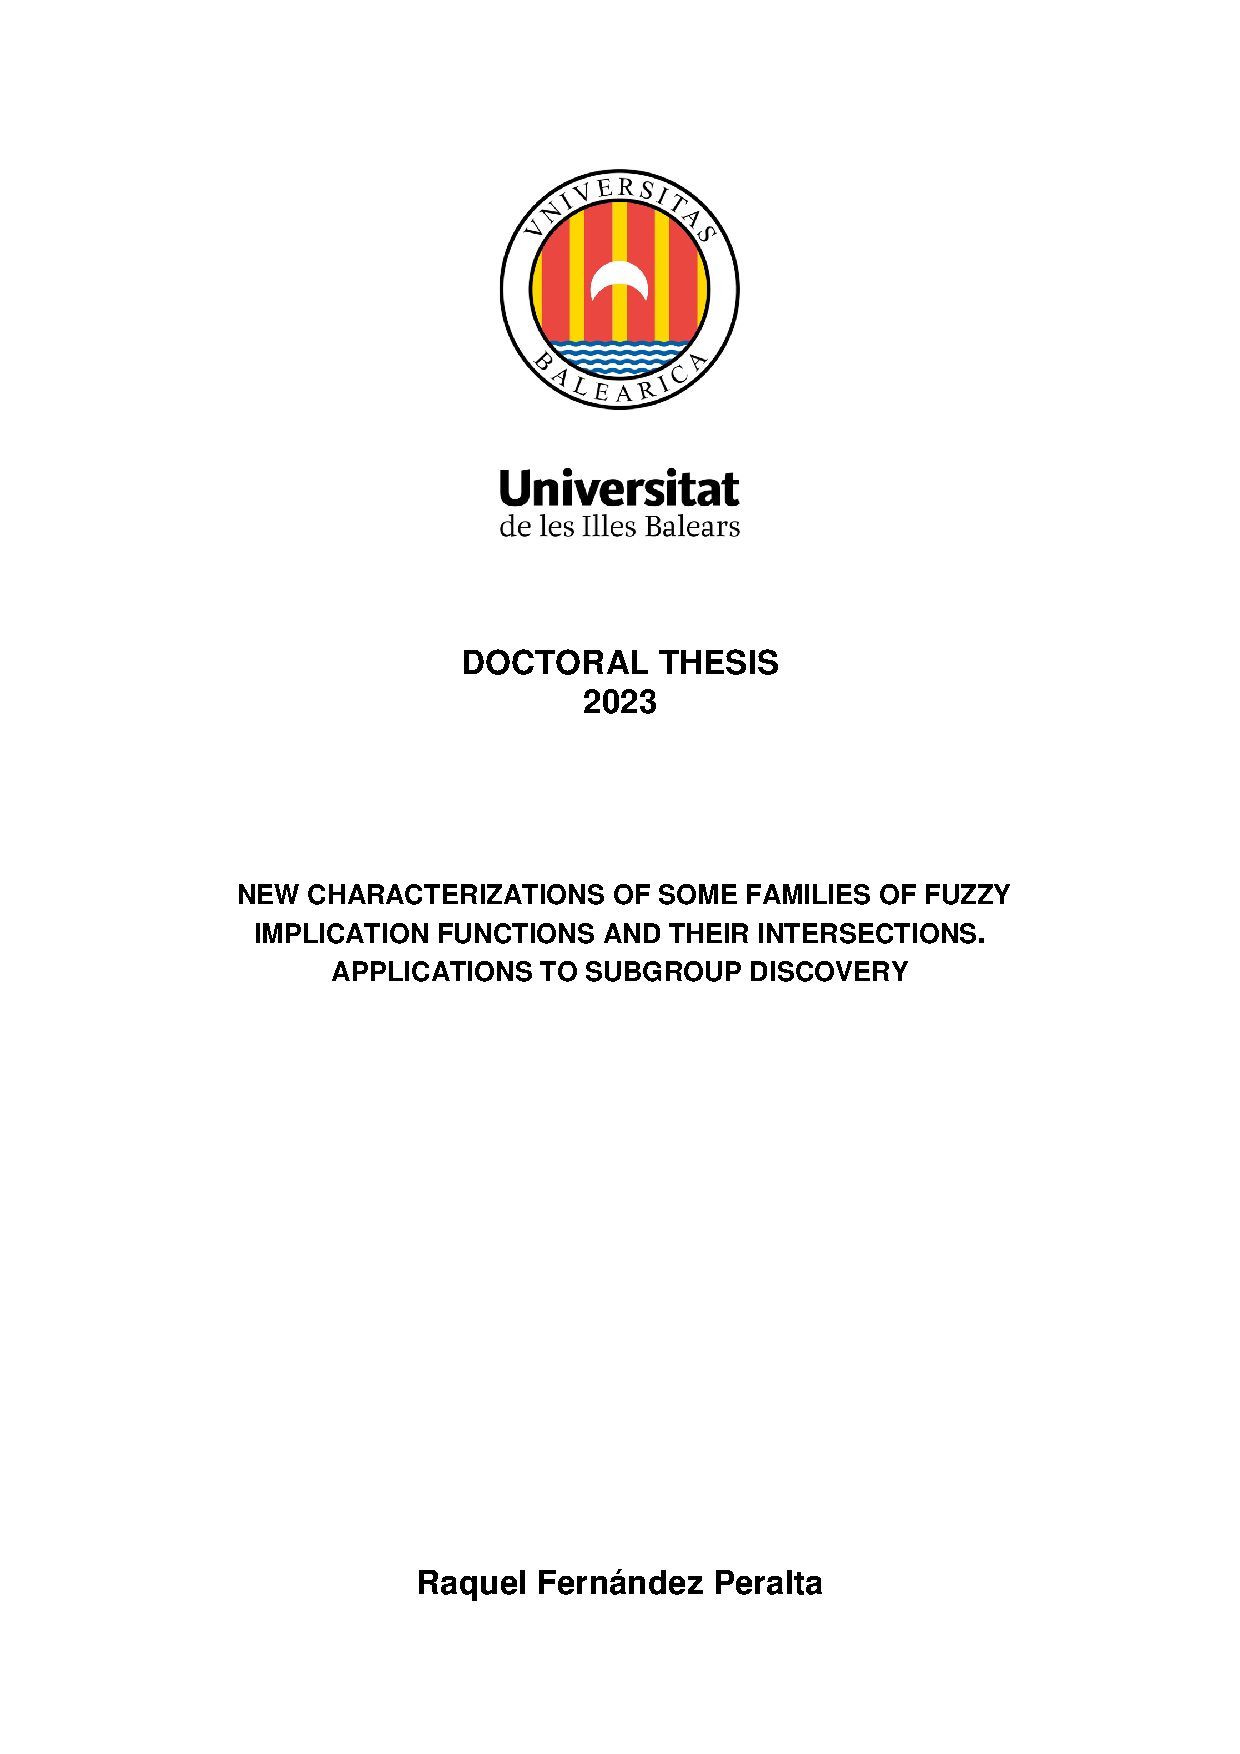
\includepdf[pages=1-1]{./Coberta/cobertaUIBsans}

\thispagestyle{empty}

\newpage $\ $

%%% ----- Portada ----- %%%

\frontmatter


\includepdf[pages=1-1]{./Portada/portadaUIBsans}
\newpage $\ $

\thispagestyle{empty}


\newpage $\ $

%%% ----- Dedication ----- %%%

\thispagestyle{empty}

\vspace*{2 in}

\begin{flushright}
	\textit{A Leo y Paco.}
\end{flushright}

\newpage $\ $

\thispagestyle{empty}

%%% ----- Abstract ----- %%%
\chapter*{Abstract}
\addcontentsline{toc}{chapter}{Abstract}

Fuzzy implication functions are one of the fundamental operators of fuzzy logic, in which they generalize the concept of the classical implication from the set $\{0,1\}$ to the unit interval $[0,1]$. The important role that these connectives play both in theory and applications has led them to become one of the most relevant research areas within fuzzy logic. In this thesis, we have mainly focused on the study and resolution of some open problems regarding the characterizations and intersections of different families.

The contents of this monograph are boldly separated into four objectives, which in turn have resulted in various contributions to the field.

To begin with, we present a characterization of generalized $(h,e)$-im\-pli\-ca\-tions. This result is obtained by first providing a representation theorem based on the horizontal threshold method that describes the structure of these operators in terms of two families which are generalizations of Yager's implications. Thus, by finding the characterizations of these two families we have transformed the representation theorem to an axiomatic characterization of generalized $(h,e)$-implications in terms of their own properties.

Second, we characterize the families of fuzzy implication functions which are invariant with respect to the positive powers of a strict/nilpotent t-norm. Further, we thoroughly study which additional properties apart from the invariance are fulfilled by these two families and we disclose that their structure stand out with respect to the most well-known families by studying the corresponding intersections.

Third, we provide significant advances on the renowned open problem of the characterization of $(S,N)$-implications when $N$ is a non-continuous fuzzy negation. We first prove that the problem is equivalent to the completion of t-conorms whose expression is unknown in a region which is determined by the discontinuities of $N$. Accordingly, we present new results on the dual problem of the completions of t-norms from which we derive a second axiomatic characterization of $(S,N)$-implications in some particular cases.

Finally, we propose a novel framework for the subgroup discovery data mining technique based on the use of fuzzy implication functions for modeling subgroups as fuzzy rules. We thoroughly describe this new setting and we study which properties should be imposed on the involved fuzzy operators. Further, we design and implement some subgroup discovery algorithms and we show that our perspective provides valuable knowledge which is different from other existing approaches.

\chapter*{Resumen}
\addcontentsline{toc}{chapter}{Resumen}

Las funciones de implicación borrosas son uno de los operadores primordiales de la lógica borrosa, en la cual generalizan el concepto de la implicación clásica del conjunto $\{0,1\}$ al intervalo unidad $[0,1]$. El importante papel que estos conectivos tienen tanto en la teoría como en las aplicaciones los ha llevado a convertirse en uno de los campos de investigación más relevantes dentro de la lógica borrosa. En esta tesis, nos hemos enfocado principalmente en el estudio y resolución de algunos problemas abiertos en relación a las caracterizaciones e intersecciones de diferentes familias.

Los contenidos de esta monografía están claramente separados en cuatro objetivos, que a su vez han resultado en varias contribuciones a este campo.

Para empezar, presentamos la caracterización de las $(h,e)$-implicaciones ge\-ne\-ra\-li\-za\-das. Este resultado se obtiene primero proporcionando un teorema de representación basado en el método del umbral horizontal, que describe la estructura de estos operadores en términos de dos familias que son generalizaciones de las implicaciones de Yager. Por consiguiente, a partir de las caracterizaciones de estas dos familias se ha transformado el teorema de representación en una caracterización axiomática de las $(h,e)$-implicaciones generalizadas con base en sus propias propiedades. 

En segundo lugar, caracterizamos las familias de funciones de implicación borrosas que son invariantes respecto de las potencias positivas de una t-norma estricta/nilpotente. Además, estudiamos en detalle qué propiedades adicionales aparte de la invariancia satisfacen estas dos familias y, a partir del estudio de las intersecciones respectivas, revelamos que su estructura destaca en relación a la de las familias más conocidas.

En tercer lugar, aportamos avances significativos al renombrado problema abierto de la caracterización de las $(S,N)$-implicaciones cuando $N$ es una negación borrosa no continua. Primero demostramos que el problema es equivalente a la completación de t-conormas cuya expresión es desconocida en una región que depende de las discontinuidades de $N$. En consecuencia, presentamos nuevos resultados del pro\-ble\-ma dual de las completaciones de t-normas, de los cuales derivamos una segunda caracterización axiomática de las $(S,N)$-implicaciones en algunos casos particulares.

Finalmente, proponemos un nuevo marco para la técnica de minería de datos de descubrimiento de subgrupos basada en el uso de funciones de implicación borrosas para modelar subgrupos como reglas borrosas. Describimos de forma detallada esta nueva configuración y estudiamos qué propiedades deberían ser impuestas en los operadores borrosos involucrados. Además, diseñamos e implementamos algunos algoritmos de descubrimiento de subgrupos y mostramos que nuestra perspectiva provee conocimiento interesante que es diferente al de otros métodos existentes.

\chapter*{Resum}
\addcontentsline{toc}{chapter}{Resum}

Les funcions d'implicació borroses són un dels operadors fonamentals de la lògica borrosa, en la qual generalitzen el concepte de la implicació clàssica del conjunt $\{0,1\}$ a l'interval unitat $[0,1]$. L'important paper que aquests connectius tenen tant a la teoria com en les aplicacions els ha duit a convertir-se en un els camps d'investigació més rellevants dins de la lògica borrosa. En aquesta tesi, ens hem enfocat principalment en l'estudi i resolució d'alguns problemes oberts en relació amb les caracteritzacions i interseccions de diferents famílies.

Els continguts d'aquesta monografia estan clarament separats en quatre objectius, que al seu torn han resultat en diverses contribucions en aquest camp.

Per començar, presentam la caracterització de les $(h,e)$-implicacions generalitzades. Aquest resultat s'obté primer proporcionant un teorema de representació basat en el mètode del llindar horitzontal, que descriu l'estructura d'aquests operadors en termes de dues famílies que són generalitzacions de les implicacions de Yager. Per consegüent, a partir de les caracteritzacions d'aquestes dues famílies s'ha transformat el teorema de representació en una caracterització axiomàtica de les $(h,e)$-implicacions generalitzades amb base en les seves pròpies propietats.


En segon lloc, caracteritzam les famílies de les funcions d'implicació borroses que són invariants respecte de les potències positives d'una t-norma estricta/nilpotent. A més, estudiam a fons quines propietats addicionals, a part de la invariància, es compleixen per aquestes dues famílies i, mitjançant l'estudi de les interseccions corresponents, revelam que la seva estructura destaca respecte de les famílies més conegudes.

En tercer lloc, proporcionam avanços significatius en el famós problema obert de la caracterització de les $(S,N)$-implicacions quan $N$ és una negació borrosa no contínua. Primer demostram que el problema és equivalent a la completació de t-conormes l'expressió de la qual és desconeguda en una regió que està determinada per les discontinuïtats de $N$. En conseqüència, presentam nous resultats sobre el problema dual de les completacions de t-normes dels quals obtenim una segona caracterització axiomàtica de les $(S,N)$-implicacions en alguns casos particulars.

Finalment, proposam un nou marc per a la tècnica de mineria de dades de descobriment de subgrups basat en l'ús de funcions d'implicació borroses per al modelatge de subgrups com a regles borroses. Descrivim a fons aquesta nova configuració i estudiam quines propietats haurien d'imposar-se als operadors borrosos implicats. A més, dissenyam i implementam alguns algorismes de descobriment de subgrups i mostram que la nostra perspectiva proporciona coneixement interessant que és diferent d'altres enfocaments existents.


% All three characterizations are based on two novel properties which are modifications of the law of importation.

%%% ----- Acknowledgments ----- %%%

\chapter*{Acknowledgments/Agradecimientos}
\addcontentsline{toc}{chapter}{Acknowledgments/Agradecimientos}

A lo largo del camino hasta aquí, he tenido la suerte de contar con el apoyo de mucha gente. Me gustaría agradecer a todos ellos ya que, de una manera u otra, me han ayudado a lograr este objetivo.

Primer de tot, vull agrair als meus directors de tesi, Arnau i Sebastià. No només m'han ajudat a tirar aquest ambiciós projecte endavant, sinó que a més sempre ho han fet des d'un tracte proper. Gràcies per tot el temps que heu invertit, per sempre valorar la meva feina, per motivar-me a fer-ho sempre el millor possible i, en general, per tot el que m'heu ensenyat durant aquests anys. Especialment, vull donar les gràcies a en Sebastià per apostar per jo d'ençà que el vaig tenir de professor a primer de carrera. No es pot entendre la meva encara curta carrera com investigadora sense el seu suport i ajuda constants durant aquests nou anys.

Gràcies a tots els membres del meu grup d'investigació, SCOPIA, pels bons moments, el seu suport i per fer-me sentir sempre part de l'equip. Per descomptat, també per haver-me deixat ocupar el seminari del grup com el meu despatx personal durant aquests quatre anys.

M'agradaria recalcar l'important paper dels professors del Grau de Matemàtiques en aquesta història. Realment, vaig entrar a la carrera sense tenir les idees gens clares, amb el sentiment d'haver-me tirat a una piscina que no sabia si estava plena. Malgrat això, des del primer curs em va apassionar aquest nou món que havia descobert. I això és degut a la gran feina de tots els professors que vaig tenir, que em varen ensenyar a estimar les matemàtiques i em varen motivar a voler dedicar-me a la investigació. Gràcies a tots aquells que sempre tengueren la porta oberta per una tutoria o un dubte, que valoraren positivament els meus progressos, que em motivaren a fer una bona feina, i que es varen esforçar per transmetre els coneixements d'una assignatura el millor possible.

También quiero agradecer a Antonio Gómez Corral, bajo la tutela del cual ya me pude iniciar en la investigación durante mis estudios de máster en la UCM. Muchos de los consejos que me dio durante esa época me han acompañado durante mi etapa de doctorado.

I would like to thank Dr. Balasubramaniam Jayaram for welcoming me with open arms during my research stay at IIT Hyderabad. The time I spent there not only helped me to start developing the results of the last chapter of my thesis, but his mentoring made me see things from a different perspective and let me grow as a researcher. Also, to Kavit, Megha and Priyanka for accompanying me on that adventure.

To Dr. Michał Baczyński, who has always shared his thoughts and advice the times we have crossed paths at a conference or during his visits to my university.

Special thanks go to Dr. Andrea Mesiarová-Zemánková for showing interest in collaborating on the problem of the completion of t-norms from the very beginning. Her explanations, examples and ideas during these four years have been crucial to the contributions in Chapter 5.

Als meus companys amb els quals he compartit el meu dia a dia durant el doctorat, Tomás, Iván, Mar, Onofre, Marco, Toni, Jordi, Biel i Cris. Al vostre costat el camí s'ha fet menys dur i molt més divertit.

A Ignasi y Lluís, por recordarme lo importante que es no dejar de hacerse preguntas y ofrecerme una mesa en Protofy siempre que he pasado por Barcelona.

Als meus amics de tota la vida, Agus, Alberto, Albertito, Dani, David, Luci, Marga, Maria, Marina, Marta, Nadine, Salva i Sara. Tenc molta sort de tenir-vos al meu costat, gràcies per tan bons moments, però també per sempre ajudar-me a tirar endavant en els moments feixucs. Esper que mai deixem de formar aquesta gran família.

A Lucas, por sus ánimos y apoyo incondicional en esta época de mi vida que ha sido como una montaña rusa, al menos siempre ha sido a tu lado.

A mis hermanos Alejandro y Antonio y a mis tíos Manolo, Antonio, Javi y Juana, gracias por el apoyo que me habéis dado durante estos años. 

Finalmente, quiero dedicar esta tesis a mis padres, porque durante toda mi vida han confiado en mí y siempre me han hecho creer que con esfuerzo podía conseguir lo que me propusiese. Sus valores y enseñanzas me han servido para llegar hasta aquí más que los de nadie.

\vspace{0.5cm}

\noindent \textbf{Financiación}\\

\noindent Esta investigación ha contado con la siguiente financiación:
\begin{itemize}
	\item La beca FPU18/05664 financiada por el Ministerio de Ciencia, Innovación y Universidades de España.
	\item La beca Movilidad EDUIB - Santander 21-22 financiada por la Escuela de Doctorado de la Universidad de las Islas Baleares y el Banco Santander.
	\item El proyecto PID2020-113870GB-I00 financiado por la Agencia Estatal de Investigación y del Ministerio de Ciencia e Innovación de España.
	\item El proyecto AEI/TIN2016-75404-P financiado por el Ministerio de Economía, Industria y Competitividad de España.
\end{itemize}


%%% ----- List of Publications ----- %%%
\pagestyle{backmatter}
\chapter*{List of Publications}
\addcontentsline{toc}{chapter}{List of Publications}

\textbf{Published Journal Papers:}
%%% Journal Papers %%%
\begin{itemize}
	\item \fullcite{Fernandez-Peralta2021}
	\item \fullcite{Fernandez-Peralta2021B}
	\item \fullcite{Fernandez-Peralta2022C}
	\item \fullcite{Fernandez-Peralta2022B}
	\item \fullcite{Fernandez-Peralta2022}
	\item \fullcite{Fernandez-PeraltaSub}
\end{itemize}

\noindent \textbf{Submitted Journal Papers:}

\begin{itemize}
	\item \fullcite{Fernandez-PeraltaSubB}
	\item \fullcite{Fernandez-PeraltaSubC}
\end{itemize}

\pagebreak

\noindent \textbf{Full Papers in Conference Proceedings:}
%%% Proceedings %%%
\begin{itemize}
	\item \fullcite{Fernandez-Peralta2018}
	\item \fullcite{Fernandez-Peralta2020}
	\item \fullcite{Baczynski2022}
	\item \fullcite{Fernandez-PeraltaSubCongC}
\end{itemize}

\noindent \textbf{Abstracts in Conference Proceedings:}
\begin{itemize}
	\item \fullcite{Fernandez-Peralta2019}
	\item \fullcite{Fernandez-Peralta2021C}
	\item \fullcite{Fernandez-Peralta2022D}
	\item \fullcite{Fernandez-PeraltaSubCongA}
	\item \fullcite{Fernandez-PeraltaSubCongB}
\end{itemize}
    
    \clearpage
    %%% ----- Table of contents ----- %%%
    \tableofcontents
    
    %%% ----- List of figures ----- %%%
    \listoffigures
    
    %%% ----- List of tables ----- %%%
    \listoftables
    
    %%% ----- List of Algorithms ----- %%%
    \listofalgorithms
	
	%%% Book main matter
    \mainmatter
    \newpage\pagestyle{main}
    %%% Chapter 1
    \chapter{Introduction}\label{chapter:introduction}
    %%%%%%%%%%%%%%%%%%%%%%%%%%%%%%%%%%%%%%%%%%%%%%%%%%%%%%%%%%%%%%%%%%%%%%
%%																	%%
%%								INTRODUCTION						%%	
%%																	%%
%%%%%%%%%%%%%%%%%%%%%%%%%%%%%%%%%%%%%%%%%%%%%%%%%%%%%%%%%%%%%%%%%%%%%%

% The end of determinism
Historically, sciences had a strict deterministic view of reality in which they assumed that every event can be completely explained by its causes. For this school of thought, any uncertainty is caused by human ignorance about what is already predetermined. For instance, Jacob Bernoulli (1654-1705) or Pierre-Simon Laplace (1749-1827), widely known for their contributions to probability theory \cite{Bernoulli1713,Laplace1812}, shared a deterministic view of the world. In the words of Pierre-Simon Laplace \cite{Laplace1902}: ``Given for one instant an intelligence which could comprehend all the forces by which nature is animated and the respective situation of the beings who compose it – an intelligence sufficiently vast to submit these data to analysis – it would embrace in the same formula the movements of the greatest bodies of the universe and those of the lightest atom; for it, nothing would be uncertain and the future, as the past, would be present to its eyes''. At the end of the 19th century and the beginning of the 20th century, several breakthroughs questioned the adequacy of strict determinism as a model of reality: Gregor Mendel's (1822-1884) experimental findings on inheritance that caused the inception of the modern age of genetics more than three decades later \cite{Gayon2016}; Ludwig Boltzmann's (1844-1906) statistical interpretation of thermodynamics \cite{Swendsen2010}; the Brownian motion empirically discovered by Robert Brown (1773-1858) and lately modeled by Louis Bachelier (1870-1946) \cite{Seth2020}; Bertrand Russell's (1872-1970) set-theoretical paradox \cite{Godehard2004}; Werner Heisenberg's (1901-1976) uncertainty principle in quantum mechanics \cite{Cassidy1992}; or Kurt Gödel's (1906-1978) incompleteness theorems \cite{Raatikainen2022}. These advances were a turning point in science history and they gave rise to a more realistic worldview in which dealing with uncertainty was the mainstay \cite{Raper2020}.

% The emergence of multivaluated logics
This new current also reached the field of mathematical logic and philosophy, in which interpreting and discussing terms like ``vagueness'' caught the attention of many scholars \cite{Russell1923,Black1937,Hempel1939}. At this point, the truth-bivalence of classical logic aroused several controversies which prompted the study of other alternatives. In \cite{Russell1923} Bertrand Russell argued that the law of excluded middle does not hold when symbols are vague and concluded that vagueness is precisely one degree of truth; Jan Łukasiewicz (1878-1956) proposed a new logic with three degrees of truth, ``true'', ``false'' and ``unknown'' \cite{Lukasiewicz1920}; Emil Leon Post (1897-1954) introduced the idea of additional truth degrees \cite{Post1921}; and Luitzen Egbertus Jan Brouwer (1881-1996) introduced intuitionistic logic as a mathematical logic where the law of excluded middle was not imposed, for which it was proved in 1932 by Gödel that it has no interpretation as a finite-valued logic \cite{Godel1932}. On the basis of these pioneering works, the branch of multi-valued logics had a thorough development in subsequent years, both in theory and applications \cite{Gottwald2001}.

% The introduction of fuzzy logic and contributions of Lofti A. Zadeh
Within this scenario, Lofti A. Zadeh (1921-2017) expressed in 1962 the necessity of a new framework for processing uncertainty \cite{Zadeh1962}:  ``...we need a radically different kind of mathematics, the mathematics of fuzzy or cloudy quantities which are not describable in terms of probability distributions.''. Three years later, he published his famous seminar paper ``Fuzzy Sets'', in which he presented a new type of sets characterized by the fact that they do not have precise boundaries and for which membership is a matter of degree \cite{Zadeh1965}. From this generalization of classical sets, he proposed a mathematical method with which processing information based on natural language descriptions like ``The temperature is high'' or ``Alex is tall'' became possible. In posterior papers \cite{Klir1996}, Zadeh developed the theory of fuzzy logic as a more adequate formalism to handle the imprecision of human reasoning \cite{Dubois2016}.

% The boom of fuzzy logic
The term ``fuzzy logic'' can be understood from two different points of view, the narrow and the wider sense \cite{Marks1994}. In the narrow sense, fuzzy logic is a multi-valued logic in which truth degrees lie within the real interval $[0,1]$, where $0$ indicates ``absolute falsity'' and 1 indicates ``absolute truth''. However, in the wider sense fuzzy logic is almost synonymous with the theory of fuzzy sets. Although fuzzy logic can be systematically studied as a multi-valued mathematical logic \cite{Hajek1998}, the utmost motive of Zadeh's ideas were to use fuzzy logic as a theory of approximate reasoning whereby truth degrees act as modifiers of the fuzzy statements they apply to. This novel theory began to flourish in industrial applications in the early 1970s, particularly in the field of expert systems \cite{Gaines1985}. Further on, in the 1980s it started the period called the ``fuzzy boom'' due to the large number of fuzzy logic based products that emerged, especially in Japan \cite{Seising2009,Garrido2012}. Indeed, some examples in which fuzzy technology was incorporated are: household appliances such as washing machines, thermostats, cameras, rice cookers, microwave ovens, air conditioners...; the Hitachi subway system in Sendai installed in 1985; vehicle's auto transmission and antiskid braking systems \cite{VonAltrock1994,Ivanov2015}; among many others \cite{Dutta1993}.

% The controversies
Although fuzzy logic had an enthusiastic reception in the East, in the West this new theory was not lacking in criticism. According to several scholars, fuzzy logic was ``content-free'' or ``probability in disguise'', pointing out that for them fuzzy logic had nothing interesting or new to offer \cite{Zadeh1996}. Zadeh did not sharpen this confrontation, since he considered that probability and fuzzy logic were complementary rather than rivals \cite{Zadeh1995}. It has been widely discussed now that fuzzy degrees of truth are not the same as probability percentages \cite{Kosko1990}. In brief, probabilities measure whether something will occur or not, and fuzziness measures the degree to which something occurs or some condition exists. For instance, the statement ``There is a 30 percent of surviving this surgery'' conveys the probability of living or dying, but ``The surgery causes 30 percent harm'' means that the process can cause harm to some extent. For a more detailed example of the difference between membership degrees and probabilities, we refer the reader to \cite{Bezdek2013}. Nowadays, fuzzy logic is a well-established discipline with several theoretical ramifications and a wide variety of contemporary application areas: computing with words \cite{Gupta2022}, fuzzy control \cite{Precup2011}, decision making \cite{Liu2020,Blanco-Mesa2017,Mardani2015}, image processing \cite{Bloch2023}, data mining and machine learning \cite{Mirzakhanov2020}, neural networks \cite{Dombi2021}, genetic algorithms \cite{Herrera2008}, knowledge discovery \cite{Ropero2011,Herrera2011,Papageorgiou2013}, medicine \cite{Uma2022}, robotics \cite{Mac2016}... 

% Fuzzy operators
One of the most important branches of fuzzy logic corresponds to the study of fuzzy operators, which are used to operate between membership values or truth degrees. Traditionally, many fuzzy concepts were defined as a generalization of the corresponding one in classical logic. Following this reasoning, the main classical logic connectives have been generalized: the intersection or conjunction is defined as a fuzzy conjunction (usually a t-norm); the union or disjunction is defined as a fuzzy disjunction (usually a t-conorm); the negation or the complement is defined as a fuzzy negation; and the conditionals are represented by fuzzy implication functions. However, the study of fuzzy operators goes beyond logic connectives and it intersects with the study of aggregation functions. Aggregation functions (also called aggregation operators) are used for combining and merging values into a single one according to a certain objective. Since fuzzy operators play an important role in a wide variety of applications, many different types have been defined. To illustrate this fact we refer the reader to some books exclusively devoted to this topic \cite{Klement2000,Calvo2002,Baczynski2008,Beliakov2010,Grabisch2009,Alsina2006}. Although other domains besides $[0,1]$ have been considered in the literature \cite{Goguen1967,Munar2023}, typically fuzzy operators are defined as functions $F:[0,1]^n \to [0,1]$ that fulfill some set of conditions (monotonicity, continuity, associativity, commutativity, boundary conditions...). However, these conditions are usually general enough to allow the existence of many different operators of a certain kind. This results in the more specific study of different classes of operators that fulfill a certain set of conditions, in which desired additional properties apart from the ones in the operator's definition can be included. Thus, from a more theoretical point of view, the study of fuzzy operators falls within the scope of functional equations \cite{Kuczma1968,Aczel1966}. This monograph is mainly devoted to the study of fuzzy implication functions from this latter perspective.

% ----- Fuzzy Implication Functions ----- %
Fuzzy implication functions are defined as functions $I:[0,1]^2 \to [0,1]$ which are decreasing with respect to the first variable, increasing with respect to the second variable and they coincide with the classical implication in $\{0,1\}^2$ \cite{Baczynski2008,Fodor1994}. In the same way boolean implications are employed in inference schemas like modus ponens, modus tollens, etc., fuzzy implication functions play a similar role in the generalization of these schemas modeling the corresponding conditionals which are called fuzzy IF-THEN rules. These rules are widely used in approximate reasoning, wherein from imprecise inputs and fuzzy premises or rules, imprecise conclusions are drawn. However, apart from inference systems based on fuzzy rules \cite{Combs1998,Jayaram2008,Jayaram2008B}, fuzzy implication functions are also considered in other application areas like fuzzy mathematical morphology or data mining \cite{Baczynski2015}.

Partly motivated by their potential applications, the study of fuzzy implication functions has significantly grown in the last decades (see the bibliometric analysis in \cite{Laenge2021}). Indeed, some monographs \cite{Baczynski2008,Baczynski2013} and surveys \cite{Mas2007,Baczynski2008B,Baczynski2015} only devoted to the study of these operators have been published. From a theoretical perspective, the main research lines in this topic focus on the definition and study of different classes of fuzzy implication functions and the additional properties that they may satisfy. 

Although the study and proposal of additional properties is also a hot topic right now \cite{Baczynski2022C,Zhou2022B,Mis2022,Dombi2021B,Baczynski2020,Baczynski2020B,Peng2020B}, let us focus on the current state of the art regarding the research on classes of fuzzy implication functions. This research line is motivated by the fact that, depending on the context and the proper rule and its behavior, various fuzzy implication functions with different properties can be adequate \cite{Trillas2008}. The most well-known families of fuzzy implication functions are the six ones collected in the surveys \cite{Mas2007,Baczynski2008B,Baczynski2015}: $(S,N)$-implications \cite{Trillas1985}, $R$-implications \cite{Trillas1985}, $QL$-implications \cite{Mas2006}, $D$-implications \cite{Mas2006}, and Yager's $f$ and $g$-implications \cite{Yager2004}. However, many other classes of fuzzy implication functions have been defined in recent years. According to the strategy used in the definition of a certain family, we can distinguish between four classes of fuzzy implication functions:
% Different classes - millor veure survey
\begin{description}
	\item[S1.] \textbf{Classes generated from other fuzzy operators such as aggregation functions, fuzzy negations, etc.:} This strategy is based on the idea of combining adequately other fuzzy operators to obtain binary functions satisfying the axioms of the definition of a fuzzy implication function. Some of the most well-known classes such as $(S,N)$, $R$, $QL$, and $D$-implications belong to this strategy since they are generated by a t-conorm and a fuzzy negation; a t-norm; or a t-norm, a t-conorm and a fuzzy negation, respectively. More recently, other families like power-based implications \cite{Massanet2017}, Sheffer Stroke implications \cite{Baczynski2022B}, probabilistic and $S$-probabilistic implications \cite{Grzegorzewski2011}, or $(T,N)$-implications \cite{Bedregal2007} have been introduced also using this strategy.
	\item[S2.] \textbf{Classes generated from unary functions:} This strategy is based on the use of univalued functions (not necessarily fuzzy negations), often additive or multiplicative generators of other fuzzy logic connectives, to construct novel classes. These functions are usually called generators of the fuzzy implication function. This strategy experienced an important boost after Yager's $f$ and $g$-generated implications were introduced in \cite{Yager2004}.
	\item[S3.] \textbf{Classes generated from other fuzzy implication functions:} Adequately modifying the expression of already given fuzzy implication functions is another popular strategy to generate novel classes of these operators. This strategy has had an important revival lately and from the classical methods of the convex linear combination, the conjugation or the max/min construction (see \cite{Baczynski2008} for further details), more complex methods and especially, ordinal sums have recently appeared.
	\item[S4.] \textbf{Classes generated according to their final expression:} This strategy is based on fixing the desired final expression of these operators, and then studying when the corresponding functions fulfill the conditions in the definition of a fuzzy implication function. As compared with the other strategies, this one is quite new and it started in 2014, when polynomial implications were presented in \cite{Massanet2014} (see \cite{Massanet2022} for a deeper study on the polynomial implications).  
\end{description}
Apart from these four strategies, the proposal of generalizations of a certain class is quite popular, that is, to define a wider family which includes the original one. For instance, in \textbf{S1} the generalizations are usually based on considering a generalization of the fuzzy operators involved; or in \textbf{S2} they are based on weakening the conditions of the unary functions used or on generalizing the operator's expression. To express the relationship between a certain family and its generalizations, we will say that the generalizations are of the same ``type''. For example, we classify the generalizations of the $(S,N)$-implications as $(S,N)$ type implications. Having said this, intending to quantify the number of families introduced in the literature so far, we have constructed Table \ref{table:families_FI}. In this table, we have counted 146 different definitions of families of fuzzy implication functions introduced in 96 references. Due to the extensive literature on the topic, there may be other families that we have missed. However, the compilation in Table \ref{table:families_FI} is significantly broader than the corresponding one in the existing surveys \cite{Mas2007,Baczynski2008B,Baczynski2015} and monographs \cite{Baczynski2008,Baczynski2013}. Nonetheless, from Table \ref{table:families_FI} we cannot conclude that there exist 146 significantly different families of fuzzy implication functions, because these families can present intersection or even coincide. For instance, the authors in \cite{Massanet2017B} proved the equivalence of two families of fuzzy implication functions through their characterization. Until that moment, the additional properties of these two families had been studied independently. For this reason, it is of the utmost importance to study the additional properties that the operators of a certain family satisfy and to provide an axiomatic characterization of the new operators in the literature in order to find its possible relation with respect to those already known. In this respect, the characterization of several families of fuzzy implication functions have already been achieved: $(S,N)$-implications with a continuous negation \cite{Baczynski2007}, $R$-implications obtained from left-continuous t-norms \cite{Miyakoshi1985,Fodor1994}, some $QL$-implications \cite{Shi2008}, Yager’s implications \cite{Massanet2012B}, $h$-implications \cite{Massanet2012A}, probabilistic and survival $S$-implications \cite{Massanet2017B}; among others \cite{Aguilo2010,Backzynski2009,Zhou2021,Massanet2019B}. Besides, the intersections between some of the families have also been studied \cite{Baczynski2008,Baczynski2008B,Backzynski2010B}. However, the majority of families in Table \ref{table:families_FI} have not been characterized yet nor its intersection with other families has been investigated. Therefore, we can conclude that the current literature on this topic is not enough to have a proper global view of all the existing families of fuzzy implication functions.

With regard to this topic, in \cite{Massanet2019C} some guidelines for decreasing the redundancy in this field and increasing the value of those classes already introduced in the literature were pointed out: to avoid proposing new classes of fuzzy implication functions without a clear motivation; to characterize those families which have not been \linebreak \enlargethispage{\baselineskip}
\begin{landscape}
	~\newline
	\begin{table}[H]
		%\centering
		\begin{center}
			\setlength\tabcolsep{7pt}
			\renewcommand{\arraystretch}{1.75} \large
			\resizebox{20cm}{!}{
				\begin{tabular}{|cc|c|c|}
					\hline
					\multicolumn{2}{|c|}{\textbf{Strategy}}                                                                                                                                                                                                                                  & \textbf{Number} & \textbf{References} \\ \hline
					\multicolumn{1}{|c|}{\multirow{9}{*}{\textbf{\begin{tabular}[c]{@{}c@{}}Generated from other \\ fuzzy operators\\ (not fuzzy implication functions)\end{tabular}}}} & \textbf{\begin{tabular}[c]{@{}c@{}}From \\ fuzzy negations\end{tabular}}                       &         5        &     \cite{Vemuri2017,Souliotis2018,Jayaram2009,Shi2010b}                \\ \cline{2-4} 
					\multicolumn{1}{|c|}{}                                                                                                                                                  & \textbf{$(S,N)$ Type } &        13         &     \cite{Trillas1985,DeBaets1999,Yager2006,Aguilo2010B,Pradera2011,Pradera2016,VemuriJayaram2012,Dimuro2014,Li2015,Li2015B,Zhou2020,Peng2020}\\ \cline{2-4}  
					\multicolumn{1}{|c|}{}                                                                                                                                                  & \textbf{$(T,N)$ Type} & 4 &\cite{Bedregal2007,Zapata2014,Hlinena2014,Pinheiro2018}\\ \cline{2-4} 
					\multicolumn{1}{|c|}{}                                                                                                                                                  & \textbf{$R$ Type}     & 12 & \cite{Trillas1985,DeBaets1999,Yager2006,Durante2007,VemuriJayaram2012,Min2016,Liu2011,Carbonell2010,Krol2011,Ouyang2012,Liu2012B,Aguilo2013,Pereira2015}\\ \cline{2-4} 
					\multicolumn{1}{|c|}{}                                                                                                                                                  & \textbf{$QL$ Type}       & 4 & \cite{Mas2006,Mas2007B,Dimuro2017,Krol2013} \\ \cline{2-4} 
					\multicolumn{1}{|c|}{}                                                                                                                                                  & \textbf{$D$ Type}        & 3 & \cite{Mas2006,Mas2007B,Dimuro2019} \\ \cline{2-4} 
					\multicolumn{1}{|c|}{}                                                                                                                                                  & \textbf{\begin{tabular}[c]{@{}c@{}}Others derived \\ from copulas\end{tabular}}                                                              &       5          &              \cite{Grzegorzewski2011,Grzegorzewski2012,Dolati2013}       \\ \cline{2-4} 
					\multicolumn{1}{|c|}{}                                                                                                                                                  & \textbf{Power-Based}         &       1          &         \cite{Massanet2017}            \\ \cline{2-4} 
					\multicolumn{1}{|c|}{}                                                                                                                                                  & \textbf{Sheffer Stroke}                                                                        &          2       &           \cite{Baczynski2022B}          \\ \hline
					\multicolumn{1}{|c|}{\multirow{2}{*}{\textbf{\begin{tabular}[c]{@{}c@{}}Generated from unary functions \\ (not fuzzy negations)\end{tabular}}}}                         & \textbf{Yager's Type} &    23             &         \cite{Yager2004,Jayaram2006,Massanet2011A,VemuriJayaram2012,Massanet2012B,Liu2012,Massanet2013B,Liu2013,Liu2013B,XieLiu2013,ZhangZhang2017,PeiZhu2017,PeiZhu2017B,Zhou2021,Zhou2022,Xie2017}            \\ \cline{2-4} 
					\multicolumn{1}{|c|}{}                                                                                                                                                  & \textbf{Others} &      18          &        \cite{Litz1996,Smutna1999,Burillo2000,Jayaram2009,Backzynski2009B,Hlinena2012,Dombi2018,Hlinena2013B,Su2015,Vemuri2017,Baczynski2020B,Backzynski2010}             \\ \hline
					\multicolumn{1}{|c|}{\multirow{2}{*}{\textbf{\begin{tabular}[c]{@{}c@{}}Generated from other \\ fuzzy implication functions \end{tabular}}}}                         & \textbf{Ordinal Sums}              &     21            &     \cite{Mesiar2004,Su2015b,Min2016,Massanet2016b,Drygas2017,Drygas2017b,Baczynski2017,Drygas2018,Drygas2018b,Baczynski2018b,DeLima2020,FernandezSanchez2023,Wang2023}                \\ \cline{2-4} 
					\multicolumn{1}{|c|}{}                                                                                                                                                  & \textbf{Others}                                                                                &          32       &           \cite{Bandler1980,Jayaram2006,Baczynski2008,Aguilo2015,ZhangPei2017,Baczynski2015B,Aguilo2018,Massanet2018,Souliotis2019,Mesiar2020,Hallam1999,Baczynski2003,VemuriJayaram2012,Massanet2012A,Massanet2013,Reiser2013,Li2017,Yi2017,Reiser2017,Su2018,Mesiar2019}          \\ \hline
					\multicolumn{2}{|c|}{\textbf{According to their final expression}}                                                                                                                                                                                                       &        3         &      \Cite{Massanet2014,Massanet2015,Massanet2016}               \\ \hline
					\multicolumn{2}{|c|}{\textbf{Total}}                                                                                                                                                                                                       &      146           &           96          \\ \hline
			\end{tabular}}
		\end{center}
		\caption{Classification of several families of fuzzy implication functions according to their construction methods. Each reference corresponds to the papers in which the corresponding families were introduced.}\label{table:families_FI}
	\end{table}
\end{landscape}

\noindent characterized yet; to solve some important open problems in the literature; and to open new application fields for fuzzy implication functions. In this monograph, we have precisely followed these guidelines.

Consequently, none of our main goals corresponds to the introduction of new classes of fuzzy implication functions or additional properties. Indeed, in general terms our principal objectives are: providing the characterization of two existing families in the literature, being one of them a well-known open problem; studying the family of fuzzy implication functions characterized by the fact that they satisfy a valuable property for approximate reasoning; and exploring the potential of fuzzy implication functions in a new application area within knowledge discovery. This is not to say that, due to the requirements of the particular problem, we do not define new families or additional properties. However, we do so with our sights focused on the main objective.

\section{Objectives, thesis structure and research contributions}

This thesis has four well-defined objectives, which have been addressed in four separate chapters. In the introduction of each corresponding chapter, a detailed contextualization of the problem is given. Therefore, in this section we only give a brief summary of the contributions linked to each objective:

\begin{description}
	\item[Objective 1.] \textit{The characterization of generalized $(h,e)$-implications.}\\
	In Chapter \ref{chapter:heimplications} the open problem of the characterization of generalized $(h,e)$-im\-pli\-ca\-tions \cite{Massanet2011A} is studied and totally solved. First of all, we study when this family fulfills some of the main additional properties of fuzzy implication functions and we obtain a representation theorem that describes the structure of a generalized $(h,e)$-implications in terms of two families of fuzzy implication functions via the horizontal threshold construction method. These two families can be interpreted as particular cases of the $(f,g)$ and $(g,f)$-implications, which are two families of fuzzy implication functions that generalize the well-known $f$ and $g$-generated implications proposed by Yager \cite{Yager2004} through a generalization of the internal factors $x$ and $\frac{1}{x}$, respectively. The additional properties of these two families are also studied in detail and the intersection between them is characterized. Subsequently, we provide the characterization of the two subfamilies of $(f,g)$ and $(g,f)$-implications that are related to the structure of generalized $(h,e)$-implications, called $(f,e)$ and $(g,e)$-implications. From these two characterizations and the representation theorem, we derive an axiomatic characterization of generalized $(h,e)$-implications. The three characterizations presented rely on two new additional properties of fuzzy implication functions which are modifications of the law of importation.
	
	\item[Objective 2.] \textit{The study of the family of fuzzy implication functions characterized by the fact that they satisfy the invariance property with respect to the positive powers of a continuous Archimedean t-norm.}
	
	The invariance property with respect to the positive powers of continuous t-norms has been recently introduced as an additional property of fuzzy implication functions which is particularly interesting in the area of approximate reasoning \cite{Massanet2017}. Although in this same paper the authors proposed power-based implications as a class of fuzzy implication functions that fulfills the invariance property with respect to many continuous t-norms, it is also pointed out that this family does not satisfy many of the most well-known additional properties of fuzzy implication functions. In Chapter \ref{chapter:tpowerinvariant} we study the invariance property in a more general way than the existing perspectives in the literature with the intention of obtaining a more versatile class of fuzzy implication functions that also satisfies this property. First, we provide the characterization of all binary functions which are invariant with respect to the positive powers of a continuous Archimedean t-norm. From this result, we define the families of strict/nilpotent $T$-power invariant implications as those classes which include all fuzzy implication functions that satisfy the invariance property with respect to a certain strict/nilpotent t-norm~$T$. We study when the members of these families do satisfy other additional properties apart from the invariance. From this study, it is proved that there are fuzzy implication functions from these two families satisfying important properties such as the exchange principle or the generalized modus ponens, among others. This analysis leads to the characterization of the intersection of these families with some of the most usual classes of fuzzy implication functions.    
	
	
	\item [Objective 3.] \textit{The characterization of $(S,N)$-implications with a non-continuous fuzzy negation.}
	
	Although the characterization of $(S,N)$-implications when $N$ is a continuous negation was presented in 2007 \cite{Baczynski2007}, the characterization in the case when $N$ is a non-continuous negation has remained one of the most significant open problems in the study of fuzzy implication functions for the last decades \cite{Baczynski2008,Baczynski2015}. In Chapter \ref{chapter:chsnimplications} we deeply analyze this problem and we provide new significant advances. Since this objective has been more laborious to study, we split our contributions in three different parts:
	\begin{itemize}
		\item[$\star$] \textit{A first characterization of $(S,N)$-implications when $N$ is a non-continuous negation. Proof of the equivalence between the characterization of $(S,N)$-implications and the problem of the completion of t-conorms.}
		
		In Section \ref{section:characterization1}  we present a general characterization of $(S,N)$-implications. From this result, we conclude that the characterization of $(S,N)$-implications where $N$ is a non-continuous fuzzy negation is equivalent to the problem of the completion of a t-conorm whose expression is unknown in a subregion of the unit square, where this subregion is determined by the discontinuities of the respective fuzzy negation. Nonetheless, we point out that to determine when a t-conorm can be completed is far from being an easy condition to verify. Thus, with the aim of providing another characterization of $(S,N)$-implications based on the explicit construction of the t-conorm $S$ we focus on the completion problem. At this point, by the duality between t-norms and t-conorms, we prove that our problem is equivalent to the study of the completions of t-norms. Thus, to be coherent with the literature on this topic \cite{Alsina2006,Klement2000} we study this dual problem.

		\item[$\star$] \textit{The characterization and construction of the continuous completions of some pre-t-norms.}
		
		The question of whether a continuous t-norm whose values in a subregion of the unit square are unknown can be (uniquely) completed is a classical and significant problem in the study of these operators \cite{Alsina2006,Klement2000}. The results regarding this topic are valuable since they disclose important information about their structure, for instance, which subregions of the domain determine the rest of the values uniquely. According to the previous item, in this report we have introduced a new motivation for the study of this well-known problem.
		
		In Section \ref{subsec:related_bibliography}, we present an overview of the results in the literature regarding the completions of t-norms. From this study we conclude that the completion problem linked to the characterization of $(S,N)$-implications is too complex to be approached in a general way. Thus, as a first step we focus on the regions derived from the case when $N$ has only one point of discontinuity and $S$ is a continuous t-conorm. In this particular case, the interest relies on the determination of the continuous completions of pre-t-norms defined on eight specific regions which, up to our knowledge, have not been previously considered in the literature. In Sections \ref{subsection:cancellative_completions} and \ref{subsection:completions_conditionalcase} we provide the continuous completions of cancellative and conditionally cancellative pre-t-norms defined on these eight regions.
		
		The obtained results are very different depending on the region and the cancellative and the conditionally cancellative situations, so several cases have had to be analyzed and a specific approach was necessary for almost each case. Depending on the case, the corresponding pre-t-norm can be completed uniquely or it has an infinite number of completions, but in all cases we provide the construction of all the continuous completions in terms of an additive generator.
		
		\item[$\star$] \textit{A second characterization of $(S,N)$-implications when $N$ has one point of discontinuity.}
		
		In Section \ref{section:characterization2} we gather the results exposed in the two above items to provide a new characterization of $(S,N)$-implications in the case when $N$ has one point of discontinuity and $S$ is the maximum or a continuous Archimedean t-conorm. In this new characterization, all the possible representations of the corresponding binary function as an $(S,N)$-implication are constructed.
		
		
	\end{itemize}
	\item[Objective 4.] \textit{The proposal of a new perspective of subgroup discovery based on fuzzy implication functions.}
	
	Subgroup discovery (SD) is a widely known descriptive data mining technique designed for identifying subgroups of data which are interesting with respect to a target variable \cite{Atzmueller2015,Helal2016}. The importance of a subgroup is numerically quantified by a quality measure, which is selected according to the objectives of the task at hand. Each subgroup is normally represented in the form of a rule $\text{Condition} \Rightarrow \text{Target}$, where ``Target'' is the property of interest and ``Condition'' is a conjunction of features. 
	One of the key aspects in SD is the interpretability of the results, so the output should be simple enough to be understood and analyzed by an expert. This requirement makes natural to consider the use of linguistic fuzzy rules to model subgroups. In accordance, several SD algorithms based on fuzzy logic have already been proposed in the literature \cite{Herrera2011}. However, up to our knowledge, these algorithms are only valid for categorical target variables and the rule form in the definition of a subgroup is interpreted as co-occurrence rather than a logical conditional. In this way, we propose a new approach that solves these two disadvantages by introducing the use of fuzzy implication functions. 
	Our contribution in Chapter \ref{chapter:sd} is to design some SD algorithms based on linguistic fuzzy rules modeled by fuzzy implication functions. Due to the structure of these operators, the corresponding subgroups can be interpreted as conditional statements and the numeric target can be modeled as a fuzzy linguistic variable. In our study, we adapt and reinterpret several SD quality measures for this new framework and we test and analyze the adequacy of the different fuzzy operators involved. 
\end{description}

The structure of this report is in line with the objectives' presentation: Chapter \ref{chapter:preliminaries} is devoted to the preliminaries, in which we introduce all the definitions and results that are necessary to understand the contributions presented in this monograph; in Chapters \ref{chapter:heimplications}, \ref{chapter:tpowerinvariant}, \ref{chapter:chsnimplications} and \ref{chapter:sd} we discuss Objectives 1, 2, 3 and 4, respectively. The report ends in Chapter \ref{chapter:conclusions} with some conclusions and future work.


    %%% Chapter 2
    \chapter{Preliminaries}\label{chapter:preliminaries}
    
\graphicspath{{./_figures/02_preliminaries/}}

\section{Notation and general results}\label{section:notation}
In this section we specify the notation used in this monograph and we point out some general results.

% Classical Logic Operators
For classical logic operations of conjunction, disjunction, negation and implication we write $\wedge$, $\vee$, $\neg$ and $\to$, respectively. 

% Crisp Sets
Let $A$ and $B$ be sets, we denote by $A \subseteq B$  when $A$ is a subset of $B$ where $A=B$ is possible; by $A \subsetneq B$ when $A$ is a proper subset of $B$; and by $A \not \subseteq B$ when $A$ is not a subset of $B$. The union, intersection, difference and Cartesian product of two sets $A$ and $B$ are denoted by $A \cup B$, $A \cap B$, $A \setminus B$ and $A \times B$, respectively. The cardinality and power set of a set $A$ are denoted by $|A|$ and $\mathcal{P}(A)$, respectively. The empty set is denoted by $\emptyset$. The complement of a subset $A \subseteq X$ is denoted by $A^c$. Given a topology on a set $A$, the topological closure, boundary and interior of $A$ are denoted by $\overline{A}$, $\partial A$, $\mathring A$, respectively.  We define $\mathbbm{1}_A : A \to \{0,1\}$ as the characteristic function of a set $A$, i.e., 
$$
\mathbbm{1}_A(x) = \left\{ \begin{array}{ll}
	1 &  \text{if }  x \in A, \\
	0 & \text{if }  x \not \in A.
\end{array}
\right.
$$
The symbol $\mathbb{N}$ denotes the set of positive integers, $\mathbb{Z}$ denotes the set of all integers, $\mathbb{R}$ denotes the set of all real numbers, and $\mathbb{N}_0 = \mathbb{N} \cup \{0\}$.

% Real sequences
A sequence of elements of a set $X$ is denoted by $\displaystyle \{a_n\}_{n \in A}$ with $A \subseteq \NN_0$ or, if $|A|$ is finite, by $\displaystyle \{a_n\}_{n=n_0}^{n_1}$ where $n$ goes from $n=n_0$ to $n=n_1$ with $n_0,n_1 \in \NN_0$.

% Functions
If $f: X \to Y$ is a function, then the domain of $f$ is denoted by $\Dom f$ and the range of $f$, i.e., the set $\{f(x) \mid x \in X\}$, is denoted by $\Ran f$. Let $A \subseteq X$ and $B \subseteq Y$, the image $f(A)$ and the preimage $f^{-1}(B)$ are defined by
$$f(A)=\{f(x) \mid x \in A\}, \quad f^{-1}(B) = \{x \in X \mid f(x) \in B\}.$$
The identity function is denoted by $\text{id}_X : X \to X$ and defined as $\text{id}_X(x)=x$ for all $x \in X$. If $A$ is a subset of $X$, then the restriction of $f$ to $A$ is defined as $\restr{f}{A} = f \circ \text{id}_A$. The composition of two functions $f : X \to Y$ and $g: U \to V$ with $Y \subseteq U$ is denoted by $g \circ f: X \to V$ and defined as $g \circ f(x)=g(f(x))$ for all $x \in X$. If a function $f: X \to Y$ is bijective then $f^{-1}: Y \to X$ denotes its inverse function and it satisfies $f^{-1}\circ f = \text{id}_X$ and  $f \circ f^{-1} = \text{id}_Y$.

% Common real functions
The floor and ceiling functions of real numbers are denoted by $\lfloor x \rfloor$ and $\lceil x \rceil$ for all $x \in \RR$, respectively. The absolute value of a real number $x \in \RR$ is denoted by $|x|$. The natural logarithm (i.e., the logarithm with respect to $e$) is denoted by $\ln(x)$ for all $x \in (0,+\infty)$, whereas the logarithm with respect to $\lambda \in (0,1) \cup (1,+\infty)$ is denoted by $\log_{\lambda}(x)$ for all $x \in (0,+\infty)$.

% Side limits
If $f:X \to \RR$ is a real function then for $a,b \in X$ the values $f(a^+)$ and $f(b^{-})$ denote the right and left-hand limits of $f$ in the points $a$ and $b$, respectively, i.e.,
$$f(a^+)= \lim_{x \to a^{+}} f(x), \quad f(b^{-})= \lim_{x \to b^{-}} f(x).$$

% Unary and Binary Operations
We denote as unary functions those that take one argument, and as binary functions those that take two arguments. Let us consider a binary function $F: X \times Y \to Z$ where $X,Y,Z \subseteq \RR$. Then, for each fixed $x_0 \in X$ the vertical section of $F$ is denoted by $F(x_0,\cdot)$. Similarly, for each fixed $y_0 \in Y$ the horizontal section of $F$ is denoted by $F(\cdot,y_0)$. These functions are defined as follows
\begin{center}
\noindent\begin{minipage}{.35\linewidth}
\begin{align*}
	F(x_0,\cdot) \colon Y & \longrightarrow Z \\[-1ex]
	y & \longmapsto F(x_0,y),
\end{align*}
\end{minipage}%
\begin{minipage}{.35\linewidth}
\begin{align*}
	F(\cdot,y_0) \colon X & \longrightarrow Z \\[-1ex]
	x & \longmapsto F(x,y_0).
\end{align*}
\end{minipage}
\end{center}

% Real Intervals
To denote a closed interval of \RR we write $[a,b]$, for an open interval $(a,b)$ and for half-open intervals $[a,b)$ or $(a,b]$. Further, we use a vertical line at the beginning or at the end of an interval to indicate that this extreme can be considered either open or closed. More specifically, if $a,b \in \mathbb{R}$ with $a<b$, then $[a,b|$ can be either $[a,b)$ or $[a,b]$ and $|a,b|$ can be either $[a,b)$, $[a,b]$, $(a,b]$ or $(a,b)$. In particular, this notation is used to simplify the number of cases in some results, in which there appear functions with one or more jump discontinuities that can either be left or right-continuous in some discontinuity points. For instance, if we consider a function $f:\mathbb{R} \to [0,1]$ given by
$$
f(x)
=\left\{ \begin{array}{ll}
	1 & \text{if } x\in [a,b|,\\
	0 &   \text{otherwise},
\end{array}
\right.
$$
we say that we are considering two types of functions, one with $f(x)=1$ if $x \in[a,b]$ and 0 otherwise, and another with $f(x)=1$ if $x \in[a,b)$ and 0 otherwise. That is to say, we consider the functions with $f(x)=1$ for all $x \in [a,b)$, $f(x)=0$ for all $x \in \mathbb{R} \setminus [a,b]$ and $f(b)\in \{0,1\}$, i.e.,  $f$ can either be left or right-continuous on $x=b$. 

% Extended real line
The extended real line $\RR \cup \{-\infty,+\infty\}$ is denoted by $[-\infty,+\infty]$ and the set $I \times I$ where $I$ is an interval, is denoted by $I^2$. The conventions when arithmetic operations are done on $+\infty$, $-\infty$ and 0 (e.g., the value of the symbols $0 \cdot (+\infty)$, $+\infty+(-\infty)$ or $\frac{0}{0}$) depend on the context and they are specified when applicable.

%Iterates of a Function
The iterates $f^{n}(x)$ of a function $f$ with $\Dom f = X$ and $\Ima f \subseteq X$ are defined recursively as follows
$$f^{0}(x)=x, \quad f^{n+1}(x)=f(f^n(x)), \quad \text{for all } x \in X, n \in \NN_0.$$
If the function $f$ is invertible, then the iterates of $f$ can also be defined for negative indices
$$f^{n-1}(x) = f^{-1}(f^{n}(x)), \quad \text{for all } x \in X, n \in \ZZ \setminus \NN.$$

% Power notation of Associative Operators
We say that a binary function $F:[a,b]^2 \to [a,b]$ with $a,b \in \RR$ is an associative operator with neutral element $e \in [a,b]$ if $F(x,F(y,z))=F(F(x,y),z)$ for all $x,y,z \in [a,b]$ and $F(x,e)=F(e,x)=x$ for all $x \in [a,b$]. In this case, the power notation $x_{F}^{(n)}$ where $n \in \mathbb{N}_0$ is defined recursively as follows 
\begin{equation}\label{eq:powers:genF}
x_{F}^{(n)}= 
\left\{ \begin{array}{ll}
	e &  \text{if } n=0, \\
	x & \text{if }  n=1,\\
	F(x,x_{F}^{(n-1)}) &  \text{if }  n>1.
\end{array}
\right.
\end{equation}

The following result simplifies the study of the continuity of binary functions $F:[0,1]^2 \to [0,1]$.

\begin{theorem}[\bf{\cite[Theorem A.0.4]{Klement2000}}]\label{theorem:A04}
	For a function $F:[0,1]^2 \to [0,1]$ which is monotonic with respect to one variable the following statements are equivalent:
	\begin{enumerate}[label=(\roman*)]
		\item $F$ is continuous.
		\item $F$ is continuous in each variable.
	\end{enumerate}
\end{theorem}

% Phi-Conjugates
By $\Phi$ we denote the family of all increasing bijections from $[0,1]$ to $[0,1]$. The conjugacy of two functions with respect to this set of functions is defined as follows.
\begin{definition}[\bf{\cite{Baczynski2008}}]
Two functions $f,g: [0,1]^n \to [0,1]$ are said to be $\Phi$-conjugate if there exists $\varphi \in \Phi$ such that $g=f_{\varphi}$ where
$$f_{\varphi}(x_1,\dots,x_n) = \varphi^{-1}(f(\varphi(x_1),\dots,\varphi(x_n))), \quad \text{for all } (x_1,\dots,x_n) \in [0,1]^n.$$
\end{definition}

% Pseudo-Inverses
In order to define a function that acts similarly to an inverse but for non-bijective functions, the concept of pseudo-inverse of monotone functions is considered.
\begin{definition}[\bf{\cite[Definition 3.2]{Klement2000}}]\label{pseudo-inverse} Let $[a,b]$ and $[c,d]$ be two closed subintervals of the extended real line $[-\infty,+\infty]$ and let $f:[a,b] \rightarrow [c,d]$ be a monotone function. Then the \emph{pseudo-inverse} $f^{(-1)}:[c,d] \rightarrow [a,b]$ is defined by
	$$f^{(-1)}(y)=\sup\{ x \in [a,b] \mid (f(x)-y)(f(b)-f(a)) <0 \}.$$
\end{definition}
If we distinguish the cases when $f$ is increasing, decreasing or a constant function in Definition \ref{pseudo-inverse}, a simpler expression for its pseudo-inverse can be obtained. In Figure \ref{fig:pseudo-inverses} there is an example of two monotone functions with their corresponding pseudo-inverses.
\begin{corollary}[\bf{\cite[Corollary 3.3]{Klement2000}}]\label{cor:pseudo-inverse}
Let $f:[a,b] \rightarrow [c,d]$ be a monotone function, where $[a,b]$ and $[c,d]$ are closed subintervals of the extended real line $[-\infty,+\infty]$.
\begin{enumerate}[label=(\roman*)]
		\item If $f(a) < f(b)$, i.e., if $f$ is increasing and non-constant, then for all $y \in [c,d]$ we obtain the simpler formula
		$$f^{(-1)}(y) = \sup \{ x \in [a,b] \mid f(x)<y \}.$$
		Moreover, the function $f^{(-1)}$ is increasing and left-continuous, and for each $y \in [c,f(a)]$ we have $f^{(-1)}(y)=a$, and for each $ y \in (f(b),d]$ we get $f^{(-1)}(y)=b$. Also, $(f^{(-1)})^{(-1)}=f$ if and only if $f$ is left-continuous and $f(a)=c$.
		\item If $f(a)>f(b)$, i.e., if $f$ is decreasing and non-constant, then for all $y \in [c,d]$ we obtain the simpler formula
		$$f^{(-1)}(y)= \sup \{ x \in [a,b] \mid f(x)>y \}.$$
		Moreover, the function $f^{(-1)}$ is decreasing and right-continuous, and for each $y \in [c,f(b)]$ we have $f^{(-1)}(y)=b$, and for each $y \in [f(a),d]$ we get $f^{(-1)}(y)=a$. Also, $(f^{(-1)})^{(-1)}=f$ if and only if $f$ is right-continuous and $f(b)=c$.
		\item If $f(a)=f(b)$, i.e., if $f$ is a constant function, then for all $y \in [c,d]$ we have $f^{(-1)}(y)=a$.
	\end{enumerate}
\end{corollary}

\begin{figure}
\centering
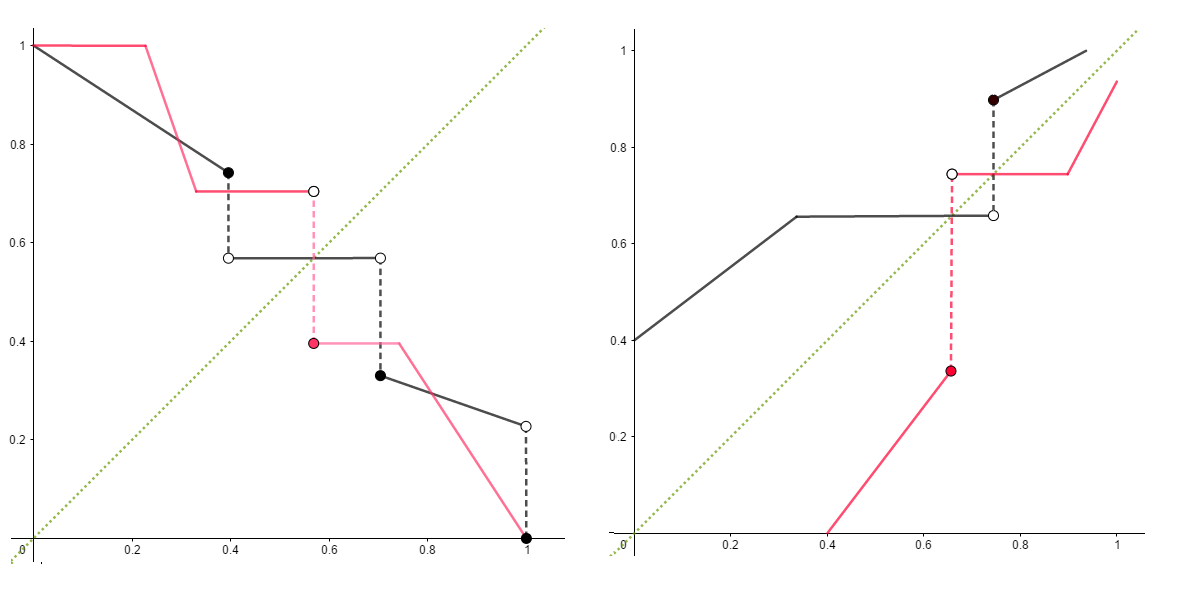
\includegraphics[scale=0.4]{pseudo-inverses.png}
\caption{A decreasing function (left) and increasing function (right) together with their respective pseudo-inverses (pink graphs).}\label{fig:pseudo-inverses}
\end{figure}


Some basic properties of the pseudo-inverse of a monotone function are recalled in the following proposition.

\begin{proposition}[\bf{\cite[Remark 3.4]{Klement2000}}]\label{prop:pseudo-inverse}
Let $f:[a,b] \rightarrow [c,d]$ be a monotone function, where $[a,b]$ and $[c,d]$ are closed subintervals of the extended real line $[-\infty,+\infty]$, and let $f^{(-1)}$ be its pseudo-inverse.
	\begin{enumerate}[label=(\roman*)]
		\item  The pseudo inverse $f^{(-1)}$ of $f$ coincides with the inverse function $f^{-1}$ of $f$ if and only if $f$ is a bijection.
		\item The pseudo inverse $f^{(-1)}$ of $f$ is continuous if and only if $f$ is strictly monotone on the set $f^{(-1)}([c,d))$.
		\item $f^{(-1)} \circ f \leq \text{id}_{[a,b]}$.
		\item The equality $f \circ f^{(-1)} \circ f = f$ holds if and only if $\displaystyle f(x_0)=\lim_{x \to x_0^{+}} f(x)$ whenever there are numbers $x_0 \in [a,b]$ and $\varepsilon >0$ such that the restriction $f\mid_{(x_0,x_0+\varepsilon]}$ is a constant function.
		\item If $f$ is strictly monotone then the restriction of $f^{(-1)}$ to Ran$(f)$, i.e., the function $f^{(-1)}\mid_{\text{Ran}(f)} : \text{Ran}(f) \rightarrow [a,b]$, is also strictly monotone. Moreover, in this case we have the following identities:
		$$ f \circ f^{(-1)} \mid_{\text{Ran}(f)} = \text{id}_{\text{Ran}(f)},$$
		$$f^{(-1)} \circ f = \text{id}_{[a,b]}.$$
		\item If $f$ is surjective then we have that $f \circ f^{(-1)} = \text{id}_{[c,d]}$.
		\item If $\varphi:[a,b] \rightarrow [a,b]$ and $\psi : [c,d] \rightarrow [c,d]$ are monotone bijections then
		$$(f \circ \varphi)^{(-1)} = \varphi^{-1} \circ f^{(-1)},$$
		$$(\psi \circ f)^{(-1)} = f^{(-1)} \circ \psi^{-1}.$$
	\end{enumerate}
\end{proposition}

Let us anticipate that some results of this monograph involve increasing functions $g:(0,1)\to [0,1]$ which are idempotent in its image except for 0 and 1. Although in the corresponding result we outline such condition by indicating that $g(z)=z$ for all $z \in \Ima g \setminus \{0,1\}$, it is easy to prove that this kind of functions are characterized by the following result.
\begin{lemma}\label{lem:idempotentfunctions} Let $g:(0,1) \to [0,1]$ be an increasing function. Then $g(z)=z$ for all $z \in \Ima g \setminus \{0,1\}$ if and only if in the interval in which $g$ is not 0 or 1, $g$ is the identity function, except for a countable set of intervals (open or closed or half-open) on which it is instead constant, taking a value which falls inside that interval.
\end{lemma}
\begin{proof}
	Let $g :(0,1) \to [0,1]$ be an increasing function. First, let us suppose that for every $z \in \Ima g \setminus \{0,1\}$ we have that $g(z)=z$. Now, consider that there exists a $y_0\in(0,1)$ such that $y_0<g(y_0)$ with $g(y_0)\in(0,1)$. Then, for all $y\in[y_0,g(y_0)]$ we have that
	$$y_0 \leq y \leq g(y_0) \Rightarrow g(y_0) \leq g(y) \leq g(g(y_0)) \Rightarrow g(y_0) \leq g(y) \leq  g(y_0) \Rightarrow g(y)=g(y_0),$$
	and we obtain that $g(y)=g(y_0)$ for all $y \in [y_0,g(y_0)]$. Analogously, it can be proved that if there exists a $y_0\in(0,1)$ such that $y_0>g(y_0)$ with $g(y_0)\in(0,1)$, then $g(y)=g(y_0)$ for all $y\in[g(y_0),y_0]$.  Thus, when we consider $y \in (0,1)$ with $g(y) \in (0,1)$ and $y \not = g(y)$, then $g(y)$ lies in an interval where $g$ is constant, taking a value which falls inside that interval. Therefore, the result follows since in this case, $g$ is the identity function, interrupted by up to countably many intervals on which $g$ is constant, taking a value which falls inside that interval.  For the reverse implication, it is straightforward to verify that if $g$ is the kind of function described above, then it is idempotent in its image except for 0 or 1.
\end{proof}
\begin{example} Some examples of increasing functions $g:(0,1) \to [0,1]$ which are idempotent in its image except for 0 and 1 are the following:
	$$ g_1(x)=x, 
	\quad 
	g_2(x)= \left\{ \begin{array}{ll}
		0 &  \text{if }  x \in \left(0,\frac{1}{4}\right), \\[3pt]
		x & \text{if }  x \in \left[\frac{1}{4},\frac{3}{4}\right],\\[3pt]
		1 &  \text{if }  x \in \left(\frac{3}{4},1\right),
	\end{array}
	\right.
	$$
	$$
	g_3(x)= \left\{ \begin{array}{ll}
		\frac{1}{4} &  \text{if }  x \in \left(0,\frac{1}{2}\right), \\[3pt]
		\frac{1}{2} & \text{if }  x \in \left[\frac{1}{2},\frac{3}{4}\right],\\[3pt]
		x &  \text{if }  x \in \left(\frac{3}{4},1\right),
	\end{array}
	\right.
	\quad
	g_4(x)= \sum_{k \geq 1} \frac{1}{2^k} \mathbbm{1}_{\left[\frac{1}{2^k},\frac{1}{2^{k-1}}\right)}(x).
	$$
\end{example}

\section{Fuzzy sets, membership functions and linguistic variables}

In this section we only provide the definitions of fuzzy set, membership function, linguistic variable and fuzzy partition. For deeper information about these concepts there are many books devoted to this topic, see for instance \cite{Cox1994,Klir1995,Zimmermann1991,Nguyen2018}.

A fuzzy set is a set whose elements have degrees of membership, and they are an extension of the classical notion of set, known as crisp set.
\begin{definition}[\bf{\cite{Zadeh1965}}]\label{def:fuzzyset}
	Let $X$ be a classical set of objects, called the \emph{universe}. A \emph{fuzzy set} $A$ of $X$ is characterized by a function $\mu_A: X \to [0,1]$, which is called the \emph{membership function} of $A$. For all $x \in X$,  the value $\mu_A(x)$ indicates the \emph{degree of membership} of $x$ in the fuzzy set $A$.
\end{definition}

The \textit{core} and \textit{support} of a fuzzy set $A$ of $X$ with membership function $\mu_A$ are defined as $C(A)= \{ x \in X \mid \mu_A(x)=1\}$ and $S(A)= \{x \in X \mid \mu_A(x)>0\}$, respectively.

In the literature, several structures of membership functions for the construction of fuzzy sets have been considered. The choice of these functions depends on the particular problem and/or application \cite{Mitaim1996}. In Example \ref{ex:mem_fun} some of the most well-known structures of membership functions are recalled.

\begin{example}\label{ex:mem_fun}
Let the universe $X$ be the set of real numbers \RR.
	\begin{itemize}
		\item Let $a \in \RR$, the corresponding \emph{singleton membership function} is defined by
		$$
		\mu_{singleton}(x;a)= \left\{ \begin{array}{ll}
			1 &  \text{if }  x =a, \\
			0 & \text{otherwise}.
		\end{array}
		\right.
		$$
		\item Let $a,b,c \in \RR$ with $a<b<c$, the corresponding \emph{triangular membership function} is defined by
		$$
		\mu_{triangular}(x;a,b,c)= \left\{ \begin{array}{ll}
			0 &  \text{if }  x \leq a, \\[3pt]
			\frac{x-a}{b-a} & \text{if }  a < x \leq b,\\[3pt]
			\frac{c-x}{c-b} &  \text{if }  b < x \leq c, \\[3pt]
			0 &  \text{if } x \geq c.
		\end{array}
		\right.
		$$
		\item Let $a,b,c,d \in \RR$ with $a<b<c<d$, the corresponding \emph{trapezoidal membership function} is defined by
				$$
		\mu_{trapezoidal}(x;a,b,c,d)= \left\{ \begin{array}{ll}
			0 &  \text{if }  x \leq a, \\[3pt]
			\frac{x-a}{b-a} & \text{if }  a < x \leq b,\\[3pt]
			1 & \text{if } b < x \leq c, \\[3pt]
			\frac{d-x}{d-c} &  \text{if }  c < x \leq d, \\[3pt]
			0 &  \text{if } x \geq d.
		\end{array}
		\right.
		$$
		\item Let $\mu, \sigma \in \RR$, the corresponding \emph{Gaussian membership function} is defined by
		$$
		\mu_{gaussian}(x;\mu,\sigma)= e^{-\frac{1}{2} \left(\frac{(x-\mu)}{\sigma}\right)^2}.
		$$
	\end{itemize}
\end{example}

A linguistic variable is a variable whose values are words or sentences in a natural or artificial language.
\begin{definition}[\bf{\cite{Zadeh1975}}]\label{def:fuzzyvariable}
	A \emph{linguistic variable} is characterized by a quintuple \linebreak $(X,T(X),U,G,\mu)$, where $X$ is the name of the variable; $T(X)$ is the set of linguistic terms of $X$; $U$ is a set called the universe of discourse; $G$ is the syntactic rule that generates the terms of $T(X)$; and $\mu$ is a semantic rule that associates the meaning with each linguistic value $X$, where $\mu(X)$ denotes a fuzzy set of $U$. For a given $X$, the name generated by $G$ is called \emph{linguistic term}.
\end{definition}
% Fuzzy partition

A fuzzy partition can be generally defined as a finite collection of fuzzy sets.  Depending on the additional conditions imposed on the fuzzy sets, different types of fuzzy partitions have been defined \cite{Bezdek1978,Dumitrescu1992,Ovchinnikov1991}. For instance, a widely-used type of fuzzy partition for real, closed intervals are Ruspini partitions.

\begin{definition}[\bf{\cite[Definition 1]{Perfilieva2006}}]
	Let $x_1 < \dots < x_n$ be fixed nodes within $[a,b]$ such that $x_1=a$, $x_n=b$ and $n \geq 2$. We say that the fuzzy sets $A_1, \dots, A_n$ establish a \emph{Ruspini partition} of $[a,b]$ if they fulfill the following conditions:
	\begin{itemize}
		\item $\mu_{A_k}: [a,b] \to [0,1]$, $\mu_{A_k}(x_k)=1$ for all $k \in \{1,\dots,n\}$;
		\item $\mu_{A_k}(x)=0$ if $x \not \in (x_{k-1},x_{k+1})$ for all $k \in \{1,\dots,n\}$, where for uniformity of notation, we set $x_0=a$ and $x_{n+1}=b$;
		\item $\mu_{A_k}$ is continuous for all $k \in \{1,\dots,n\}$;
		\item If $k \in \{2,\dots,n\}$ then $\mu_{A_k}(x)$ is strictly increasing on $[x_{k-1},x_k]$;
		\item If $k \in \{1,\dots,n-1\}$ then $\mu_{A_k}(x)$ is strictly decreasing on $[x_k,x_{k+1}]$;
		\item $\displaystyle \sum_{k=1}^n \mu_{A_k}(x)=1$, for all $x \in [a,b]$.
 	\end{itemize}
\end{definition}

In practical terms, for each linguistic variable involved in a concrete problem usually a fuzzy partition of its domain is considered (see Figure \ref{fig:example_linguistic_label}).

\begin{figure}[H]
	\centering
\tikzset{every picture/.style={line width=0.75pt}} %set default line width to 0.75pt        

\begin{tikzpicture}[x=0.75pt,y=0.75pt,yscale=-1,xscale=1]
	%uncomment if require: \path (0,300); %set diagram left start at 0, and has height of 300
	
	%Rounded Rect [id:dp5043193231595386] 
	\draw   (220.35,26.26) .. controls (220.35,22.8) and (223.15,20) .. (226.61,20) -- (313.17,20) .. controls (316.63,20) and (319.43,22.8) .. (319.43,26.26) -- (319.43,45.03) .. controls (319.43,48.48) and (316.63,51.29) .. (313.17,51.29) -- (226.61,51.29) .. controls (223.15,51.29) and (220.35,48.48) .. (220.35,45.03) -- cycle ;
	
	%Straight Lines [id:da7800093448947967] 
	\draw    (270.43,51.29) -- (186.32,80.63) ;
	\draw [shift={(184.43,81.29)}, rotate = 340.77] [color={rgb, 255:red, 0; green, 0; blue, 0 }  ][line width=0.75]    (10.93,-3.29) .. controls (6.95,-1.4) and (3.31,-0.3) .. (0,0) .. controls (3.31,0.3) and (6.95,1.4) .. (10.93,3.29)   ;
	%Straight Lines [id:da4016471229943066] 
	\draw    (270.43,51.29) -- (230.04,81.1) ;
	\draw [shift={(228.43,82.29)}, rotate = 323.57] [color={rgb, 255:red, 0; green, 0; blue, 0 }  ][line width=0.75]    (10.93,-3.29) .. controls (6.95,-1.4) and (3.31,-0.3) .. (0,0) .. controls (3.31,0.3) and (6.95,1.4) .. (10.93,3.29)   ;
	%Straight Lines [id:da2825911929820748] 
	\draw    (270.43,51.29) -- (270.43,79.29) ;
	\draw [shift={(270.43,81.29)}, rotate = 270] [color={rgb, 255:red, 0; green, 0; blue, 0 }  ][line width=0.75]    (10.93,-3.29) .. controls (6.95,-1.4) and (3.31,-0.3) .. (0,0) .. controls (3.31,0.3) and (6.95,1.4) .. (10.93,3.29)   ;
	%Straight Lines [id:da9535710275229592] 
	\draw    (270.43,51.29) -- (321.7,81.28) ;
	\draw [shift={(323.43,82.29)}, rotate = 210.32] [color={rgb, 255:red, 0; green, 0; blue, 0 }  ][line width=0.75]    (10.93,-3.29) .. controls (6.95,-1.4) and (3.31,-0.3) .. (0,0) .. controls (3.31,0.3) and (6.95,1.4) .. (10.93,3.29)   ;
	%Straight Lines [id:da3867224952909125] 
	\draw    (270.43,51.29) -- (369.5,78.75) ;
	\draw [shift={(371.43,79.29)}, rotate = 195.49] [color={rgb, 255:red, 0; green, 0; blue, 0 }  ][line width=0.75]    (10.93,-3.29) .. controls (6.95,-1.4) and (3.31,-0.3) .. (0,0) .. controls (3.31,0.3) and (6.95,1.4) .. (10.93,3.29)   ;
	%Shape: Axis 2D [id:dp9498815687860906] 
	\draw  (156,220.69) -- (395,220.69)(179.9,122.33) -- (179.9,231.62) (388,215.69) -- (395,220.69) -- (388,225.69) (174.9,129.33) -- (179.9,122.33) -- (184.9,129.33)  ;
	%Straight Lines [id:da20391340899144117] 
	\draw    (180.43,150.62) -- (240.2,220.93) ;
	%Straight Lines [id:da5667233317973046] 
	\draw    (210.2,220.93) -- (240.2,150.93) ;
	%Straight Lines [id:da7732667640639663] 
	\draw    (279.2,220.93) -- (240.2,150.93) ;
	%Straight Lines [id:da7170851127463433] 
	\draw    (240.2,220.93) -- (270.2,150.93) ;
	%Straight Lines [id:da03498652326961316] 
	\draw    (309.2,220.93) -- (270.2,150.93) ;
	%Straight Lines [id:da8429969469846545] 
	\draw    (279.2,219.93) -- (309.2,149.93) ;
	%Straight Lines [id:da9649226998275144] 
	\draw    (348.2,219.93) -- (309.2,149.93) ;
	%Straight Lines [id:da42538415289147746] 
	\draw    (310.2,220.93) -- (340.2,150.93) ;
	%Straight Lines [id:da2789076103705388] 
	\draw    (374,151) -- (340.2,150.93) ;
	%Straight Lines [id:da17676732587924837] 
	\draw  [dash pattern={on 0.84pt off 2.51pt}]  (179.33,102.33) -- (192.99,148.75) ;
	\draw [shift={(193.56,150.67)}, rotate = 253.6] [color={rgb, 255:red, 0; green, 0; blue, 0 }  ][line width=0.75]    (10.93,-3.29) .. controls (6.95,-1.4) and (3.31,-0.3) .. (0,0) .. controls (3.31,0.3) and (6.95,1.4) .. (10.93,3.29)   ;
	%Straight Lines [id:da9172065472117523] 
	\draw  [dash pattern={on 0.84pt off 2.51pt}]  (225.33,102) -- (239.36,143.77) ;
	\draw [shift={(240,145.67)}, rotate = 251.43] [color={rgb, 255:red, 0; green, 0; blue, 0 }  ][line width=0.75]    (10.93,-3.29) .. controls (6.95,-1.4) and (3.31,-0.3) .. (0,0) .. controls (3.31,0.3) and (6.95,1.4) .. (10.93,3.29)   ;
	%Straight Lines [id:da20807959196798587] 
	\draw  [dash pattern={on 0.84pt off 2.51pt}]  (273.33,102.33) -- (273.33,144.33) ;
	\draw [shift={(273.33,146.33)}, rotate = 270] [color={rgb, 255:red, 0; green, 0; blue, 0 }  ][line width=0.75]    (10.93,-3.29) .. controls (6.95,-1.4) and (3.31,-0.3) .. (0,0) .. controls (3.31,0.3) and (6.95,1.4) .. (10.93,3.29)   ;
	%Straight Lines [id:da6557057175466074] 
	\draw  [dash pattern={on 0.84pt off 2.51pt}]  (324,102.33) -- (310.63,142.44) ;
	\draw [shift={(310,144.33)}, rotate = 288.43] [color={rgb, 255:red, 0; green, 0; blue, 0 }  ][line width=0.75]    (10.93,-3.29) .. controls (6.95,-1.4) and (3.31,-0.3) .. (0,0) .. controls (3.31,0.3) and (6.95,1.4) .. (10.93,3.29)   ;
	%Straight Lines [id:da5598108462458484] 
	\draw  [dash pattern={on 0.84pt off 2.51pt}]  (370,102.33) -- (356.63,142.44) ;
	\draw [shift={(356,144.33)}, rotate = 288.43] [color={rgb, 255:red, 0; green, 0; blue, 0 }  ][line width=0.75]    (10.93,-3.29) .. controls (6.95,-1.4) and (3.31,-0.3) .. (0,0) .. controls (3.31,0.3) and (6.95,1.4) .. (10.93,3.29)   ;
	
	% Text Node
	\draw (142,84) node [anchor=north west][inner sep=0.75pt]   [align=left] {\{ very low, low, medium, high, very high \}};
	% Text Node
	\draw (228.72,27.02) node [anchor=north west][inner sep=0.75pt]   [align=left] {Price Coffee};
	% Text Node
	\draw (329,29) node [anchor=north west][inner sep=0.75pt]  [font=\scriptsize,color={rgb, 255:red, 128; green, 128; blue, 128 }  ,opacity=1 ] [align=left] {Name of Linguistic Variable};
	% Text Node
	\draw (347,56.67) node [anchor=north west][inner sep=0.75pt]  [font=\scriptsize,color={rgb, 255:red, 128; green, 128; blue, 128 }  ,opacity=1 ] [align=left] {Syntactic Rule};
	% Text Node
	\draw (398.33,212.73) node [anchor=north west][inner sep=0.75pt]    {$U$};
	% Text Node
	\draw (445,87.33) node [anchor=north west][inner sep=0.75pt]  [font=\scriptsize,color={rgb, 255:red, 128; green, 128; blue, 128 }  ,opacity=1 ] [align=left] {Linguistic Terms};
	% Text Node
	\draw (381,118) node [anchor=north west][inner sep=0.75pt]  [font=\scriptsize,color={rgb, 255:red, 128; green, 128; blue, 128 }  ,opacity=1 ] [align=left] {Semantic Rule};
	% Text Node
	\draw (383.67,175.33) node [anchor=north west][inner sep=0.75pt]  [font=\scriptsize,color={rgb, 255:red, 128; green, 128; blue, 128 }  ,opacity=1 ] [align=left] {Fuzzy Partition};
\end{tikzpicture}
\caption{Conceptual example of a linguistic variable ``Price Coffee''.}\label{fig:example_linguistic_label}
\end{figure}
\section{Fuzzy negations, t-norms, t-conorms, uninorms and copulas}

In this section we introduce some of the main operators of fuzzy logic: fuzzy negations, t-norms, t-conorms, uninorms and copulas.

\subsection{Fuzzy negations}
A fuzzy negation $N$ is a generalization of the classical negation $\neg$, whose truth table is defined by the conditions: $\neg 0=1$ and $\neg 1 =0$.
\begin{definition}[\bf{\cite[Definition 1.1]{Fodor1994}}]\label{def:fuzzy_negation}
	A unary function $N:[0,1] \to [0,1]$ is said to be a \emph{fuzzy negation} if it satisfies:
	\begin{description}
		\item[(N1)] $N(0)=1$ and $N(1)=0$. \hfill (Boundary Condition)
		\item[(N2)] $N$ is decreasing. \hfill (Monotonicity)
	\end{description}
\end{definition}
In Definition \ref{def:fuzzy_negation}, the property {\bf (N1)} imposes the boundary conditions of the classical negation and {\bf (N2)} points out that as the belongingness of an element to one set increases, its belongingness to the complement set decreases. Since the definition of a fuzzy negation is wide, other restrictions on this kind of functions have been introduced in the literature.
\begin{definition}[\bf{\cite{Fodor1994}}] A fuzzy negation $N$ is called
	\begin{enumerate}[label=(\roman*)]
		\item  \emph{strict} if it satisfies:
		\begin{description}
			\item[(N3)] $N$ is strictly decreasing.
			\item[(N4)] $N$ is continuous.
		\end{description}
		\item \emph{strong} if it is an involution, i.e., if it satisfies:
		\begin{description}
			\item[(N5)] $N(N(x))=x$ for all $x \in [0,1]$.
		\end{description}
		\item \emph{non-vanishing} if ($N(x)=0 \Leftrightarrow x=1$).
		\item \emph{non-filling} if ($N(x)=1 \Leftrightarrow x=0$).
	\end{enumerate}
\end{definition}

\begin{corollary}[\bf{\cite[Corollary 1.4.6]{Baczynski2008}}]
	Every strong fuzzy negation is strict. Every strict negation is non-vanishing and non-filling.
\end{corollary}

In Table \ref{table:fuzzy_negations} examples of well-known fuzzy negations can be found. Moreover, in Figure \ref{fig:sugeno_negation} there is the plot of some fuzzy negations in the Sugeno class for different values of $\lambda$.
\begin{table}[ht!]
	\setlength\tabcolsep{5pt}
	\renewcommand{\arraystretch}{1.5}
	\centering
	\begin{tabular}{|c|l|l|} \hline
		\bf Name & \multicolumn{1}{|c|}{\bf Formula} & \multicolumn{1}{|c|}{\bf Properties} \\[2pt]  
		\hline \bf Classic & $\NC(x)=1-x$ & strong \\[2pt] 
		\hline \bf G\"odel negation  & $\NDOne(x)=\left\{\begin{array}{ll}1&\hbox{if } x=0\\0&\hbox{if } x\in(0,1]\end{array}\right.$ & non-filling\\[2pt] 
		\hline \bf Greatest & $\NDTwo(x)=\left\{\begin{array}{ll}1&\hbox{if } x\in[0,1)\\0&\hbox{if } x=1\end{array}\right.$ & non-vanishing  \\[2pt] 
		\hline - & $N_{\bf K}(x)=1-x^2$ & strict  \\[2pt] 
		\hline - & $N_{\bf R}(x)=1-\sqrt{x}$ & strict  \\[2pt] 
		\hline \bf Sugeno class & $N^{\lambda}(x)=\frac{1-x}{1-\lambda x}, \quad \lambda \in (-\infty,1)$ & strong  \\[2pt] 
		\hline \bf Yager class & $N^{w}(x)=(1-x^w)^{\frac{1}{w}}, \quad w \in (0,+\infty)$ & strong  \\
		\hline
	\end{tabular}
	\caption{Basic Fuzzy Negations.}\label{table:fuzzy_negations}
\end{table}

\begin{figure}[ht!]
	\centering
	\begin{tikzpicture}
		\draw[scale=4,->] (-0.1, 0) -- (1.1, 0) node[right] {$x$};
		\draw[scale=4,->] (0, -0.1) -- (0, 1.1) node[above] {$N^{\lambda}$};
		\node at (0.4,0.4) [above,rotate=-45]  {\tiny $\lambda=-100$};
		\node at (0.9,0.9) [above,rotate=-45]  {\tiny $\lambda=-10$};
		\node at (1.6,1.6) [above,rotate=-45]  {\tiny $\lambda=-1$};
		\node at (1.95,1.95) [above,rotate=-45]  {\tiny $\lambda=0$};
		\node at (2.29,2.29) [above,rotate=-45]  {\tiny $\lambda=0.5$};
		\node at (2.6,2.6) [above,rotate=-45]  {\tiny $\lambda=0.75$};
		\node at (2.97,2.97) [above,rotate=-45]  {\tiny $\lambda=0.9$};
		\node at (3.59,3.59) [above,rotate=-45]  {\tiny $\lambda=0.99$};
		\draw[scale=4,samples=1000, domain=0:1, smooth, variable=\x, black] plot ({\x}, {(1-\x)/(1-0.99*\x)});
		\draw[scale=4,samples=1000, domain=0:1, smooth, variable=\x, black] plot ({\x}, {(1-\x)/(1-0.9*\x)});
		\draw[scale=4,samples=1000, domain=0:1, smooth, variable=\x, black] plot ({\x}, {(1-\x)/(1-0.75*\x)});
		\draw[scale=4,samples=1000, domain=0:1, smooth, variable=\x, black] plot ({\x}, {(1-\x)/(1-0.5*\x)});
		\draw[scale=4,samples=1000, domain=0:1, smooth, variable=\x, black] plot ({\x}, {(1-\x)/(1-0*\x)});
		\draw[scale=4,samples=1000, domain=0:1, smooth, variable=\x, black] plot ({\x}, {(1-\x)/(1+1*\x)});
		\draw[scale=4,samples=1000, domain=0:1, smooth, variable=\x, black] plot ({\x}, {(1-\x)/(1+10*\x)});
		\draw[scale=4,samples=1000, domain=0:1, smooth, variable=\x, black] plot ({\x}, {(1-\x)/(1+100*\x)});
	\end{tikzpicture}
	\caption{Plot of $N^{\lambda}$ for $\lambda \in \{-100,-10,-1,0,0.5,0.75,0.9,0.99\}$.}\label{fig:sugeno_negation}
\end{figure}

Since a fuzzy negation is a monotone function, we can define its pseudo-inverse (see Definition \ref{pseudo-inverse} and Corollary \ref{cor:pseudo-inverse}). However, the pseudo-inverse may not be a fuzzy negation (it may not satisfy the boundary conditions). To solve this problem, the modified pseudo-inverse of a fuzzy negation is considered.

\begin{definition}[\bf{\cite{Baczynski2007}}]
	Let $N$ be a fuzzy negation, the \emph{modified pseudo-inverse} of $N$ is denoted by $\mathfrak{R}_N$ and it is defined as follows
	\begin{equation}\label{eq:modified_pseudoinverse_negation}
		\mathfrak{R}_N(x)
		=
		\left\{ \begin{array}{ll}
			1 &   \text{if }   x=0, \\
			N^{(-1)}(x) & \text{if } x \in (0,1], \\
		\end{array} \right.
	\end{equation}
	where $N^{(-1)}$  is the pseudo-inverse of $N$ given by
	$$N^{(-1)}(x)=\sup \{y \in [0,1] \, | \, N(y)>x\}, \quad \text{for all } x \in [0,1].$$
\end{definition}

\begin{proposition}[\bf{\cite[Proposition 3.13]{Baczynski2007}}]\label{prop:properties_modifiedpseudoinverse}
	Let $N$ be a continuous fuzzy negation and $\mathfrak{R}_N$ its modified pseudo-inverse. Then, the following statements hold:
	\begin{enumerate}[label=(\roman*)]
		\item $\mathfrak{R}_N$ is a fuzzy negation.
		\item $\mathfrak{R}_N$ is a strictly decreasing function.
		\item 
		\begin{equation}\label{eq:PropositionRN(iii)}
			N \circ \mathfrak{R}_N = \text{id}_{[0,1]}.
		\end{equation}
		\item \begin{equation}\label{eq:PropositionRN(iv)}		
			\mathfrak{R}_N \circ N |_{\Ran \mathfrak{R}_N} = \text{id}_{\Ran \mathfrak{R}_N}.
		\end{equation}
	\end{enumerate}
\end{proposition}	

\subsection{Triangular norms and triangular conorms}

Fuzzy conjunctions and fuzzy disjunctions are the operators in fuzzy logic which play a similar role to the classical conjunctions and disjunctions in binary logic. They are defined as increasing functions $C,D:[0,1]^2 \to [0,1]$ such that $C(0,1)=C(1,0)=0$ and $D(0,1)=D(1,0)=1$, respectively. Although many different families have been introduced (see \cite{Beliakov2010,Calvo2002,Grabisch2009}), the most widely-known ones are t-norms and t-conorms.

Triangular norms, also called t-norms, and triangular conorms, also called t-conorms, are a kind of associative, binary operations originated and widely studied in the framework of probabilistic metric spaces. However, in fuzzy logic t-norms and t-conorms usually play the role of the generalization of the classical conjunction and disjunction, respectively.
\begin{definition}[\bf{\cite{Klement2000,Menger1942}}]\label{def:tnorm}
	A binary operator $T:[0,1]^2 \to [0,1]$ is said to be a \emph{triangular norm} (or \emph{t-norm} for short) if it satisfies:
	\begin{description}
		\item[(T1)] $T(x,y)=T(y,x)$ for all $x,y \in [0,1]$. \hfill (Commutativity)
		\item[(T2)] $T(x,T(y,z))=T(T(x,y),z)$ for all $x,y,z \in [0,1]$. \hfill (Associativity)
		\item[(T3)] $T(x,y) \leq T(x,z)$ when $y \leq z$, for all $x,y,z \in [0,1]$. \hfill (Monotonicity)
		\item[(T4)] $T(x,1)=x$ for all $x \in [0,1]$. \hfill (Boundary Condition)
	\end{description}
\end{definition}


\begin{definition}[\bf{\cite{Klement2000,Schweizer1961}}]\label{def:tconorm}
	A binary operator $S:[0,1]^2 \to [0,1]$ is said to be a \emph{triangular conorm} (or \emph{t-conorm} for short) if it satisfies:
	\begin{description}
		\item[(S1)] $S(x,y)=S(y,x)$ for all $x,y \in [0,1]$. \hfill (Commutativity)
		\item[(S2)] $S(x,S(y,z))=S(S(x,y),z)$ for all $x,y,z \in [0,1]$. \hfill (Associativity)
		\item[(S3)] $S(x,y) \leq S(x,z)$ when $y \leq z$, for all $x,y,z \in [0,1]$. \hfill (Monotonicity)
		\item[(S4)] $S(x,0)=x$ for all $x \in [0,1]$. \hfill (Boundary Condition)
	\end{description}
\end{definition}

From Definitions \ref{def:tnorm} and \ref{def:tconorm} it is obvious that t-norms and t-conorms behave such as the classical conjunction and disjunction when they are restricted to $\{0,1\}^2$. Notice that the only difference between the axioms of a t-norm and a t-conorm is the neutral element. In Tables \ref{table:basic_tnorms} and  \ref{table:basic_toconorms} examples of t-norms and t-conorms can be found. Moreover, in Figures \ref{fig:basic_tnorms} and \ref{fig:basic_tconorms} there is the plot of these examples.

\begin{table}[ht!]
	\setlength\tabcolsep{5pt}
	\renewcommand{\arraystretch}{1.5}
	\centering
	\begin{tabular}{|c|l|}
		\hline
		\bf Name              & \multicolumn{1}{c|}{\bf Formula}                                                                                           \\ \hline
		\bf minimum           & $T_{\bm M}(x,y)=\min\{x,y\}$                                                                                             \\ \hline
		\bf algebraic product & $T_{\bm P}(x,y)=xy$                                                                                                    \\ \hline
		\bf {\L}ukasiewicz       & $T_{\bm LK}(x,y)=\max\{x+y-1,0\}$                                                                                        \\ \hline
		\bf drastic product   & $T_{\bm D}(x,y)=\left\{\begin{array}{ll}0 &\hbox{if } x,y \in [0,1)\\\min\{x,y\}&\hbox{otherwise}\end{array}\right.$ \\ \hline
		\bf nilpotent minimum & $T_{\bm nM}(x,y)=\left\{\begin{array}{ll}0 &\hbox{if } x+y \leq 1\\\min\{x,y\}&\hbox{otherwise}\end{array}\right.$   \\ \hline
	\end{tabular}
	\caption{Basic t-norms.}
	\label{table:basic_tnorms}
\end{table}
\begin{table}[ht!]
	\setlength\tabcolsep{5pt}
	\renewcommand{\arraystretch}{1.5}
	\centering
	\begin{tabular}{|c|l|}
		\hline
		\bf Name              & \multicolumn{1}{c|}{\bf Formula}                                                                                           \\ \hline
		\bf maximum           & $S_{\bm M}(x,y)=\max\{x,y\}$                                                                                             \\ \hline
		\bf probabilistic sum & $S_{\bm P}(x,y)=x+y-xy$                                                                                                \\ \hline
		\bf {\L}ukasiewicz       & $S_{\bm LK}(x,y)=\min\{x+y,1\}$                                                                                          \\ \hline
		\bf drastic sum       & $S_{\bm D}(x,y)=\left\{\begin{array}{ll}1 &\hbox{if } x,y \in (0,1]\\\max\{x,y\}&\hbox{otherwise}\end{array}\right.$ \\ \hline
		\bf nilpotent maximum & $S_{\bm nM}(x,y)=\left\{\begin{array}{ll}1 &\hbox{if } x+y \geq 1\\\max\{x,y\}&\hbox{otherwise}\end{array}\right.$   \\ \hline
	\end{tabular}
	\caption{Basic t-conorms.}
	\label{table:basic_toconorms}
\end{table}

\begin{figure}[ht!]
	\centering
	\begin{subfigure}{.3\textwidth}
		\centering
		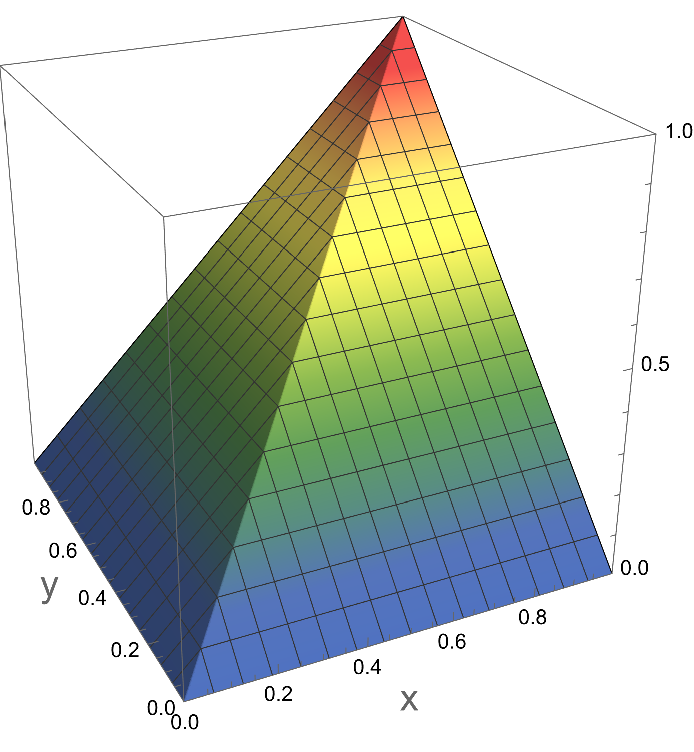
\includegraphics[scale=0.35]{TM.pdf}
		\caption{\TM}
	\end{subfigure}\hspace{0.5cm}
	\begin{subfigure}{.3\textwidth}
		\centering
		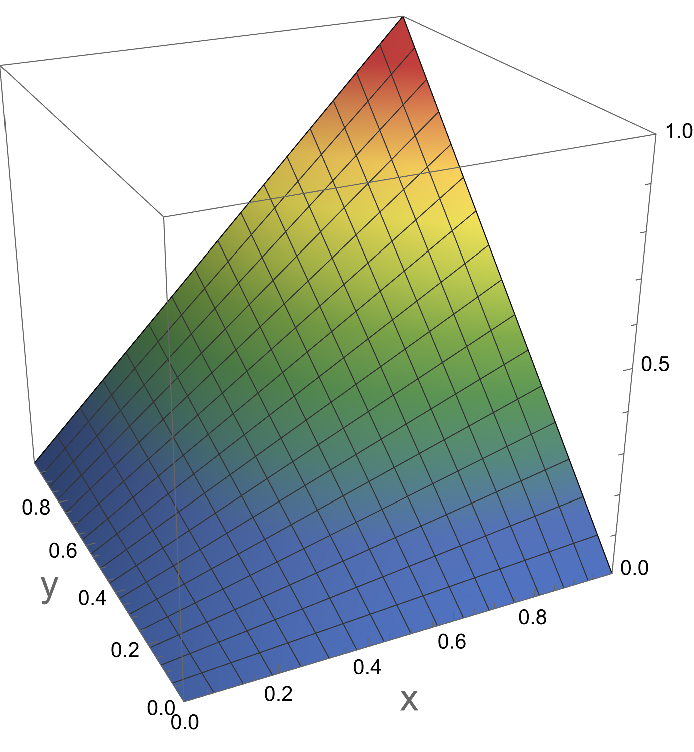
\includegraphics[scale=0.35]{TP.pdf}
		\caption{\TP}
	\end{subfigure}\hspace{0.5cm}
		\begin{subfigure}{.3\textwidth}
		\centering
		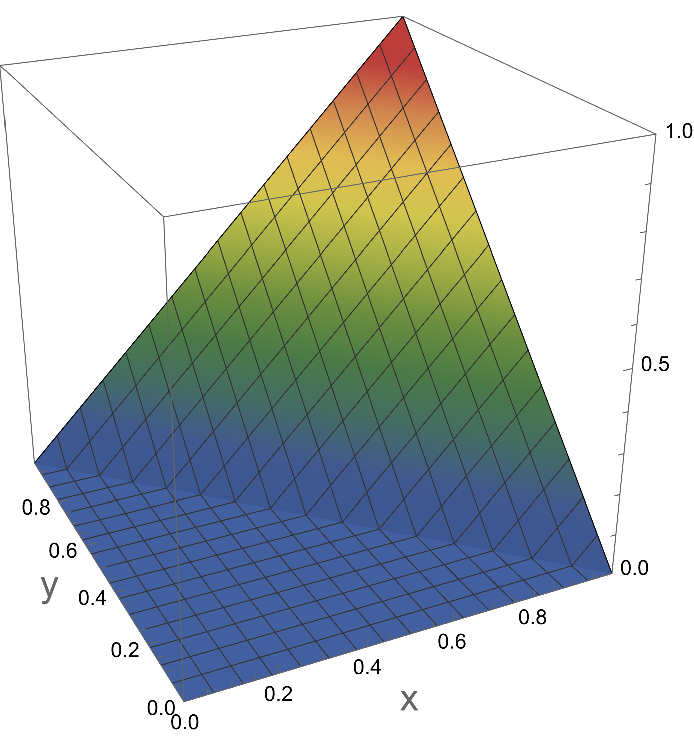
\includegraphics[scale=0.35]{TLK.pdf}
		\caption{\TLK}
	\end{subfigure}\\
	\hspace{0.25cm}
	\begin{subfigure}{.4\textwidth}
		\centering
		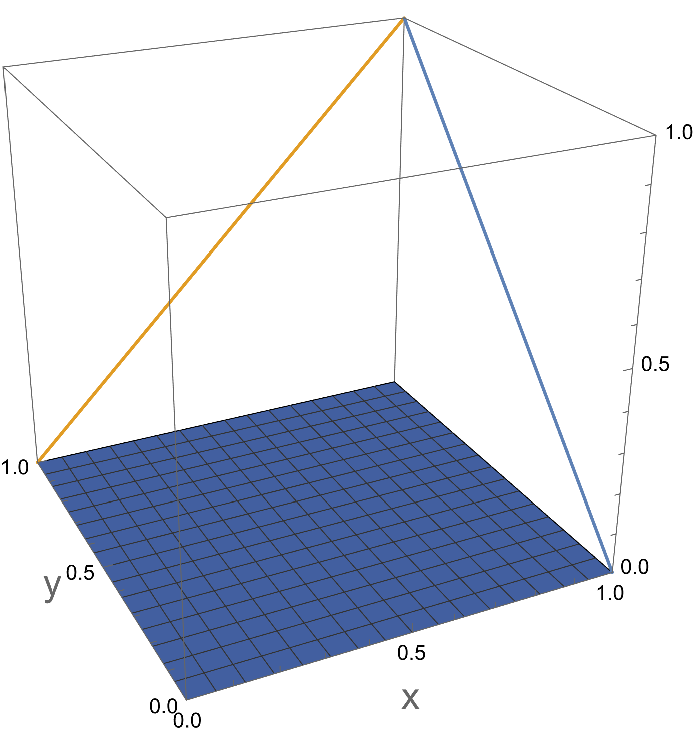
\includegraphics[scale=0.35]{TD.pdf}
		\caption{\TD}
	\end{subfigure}\hspace{0.25cm}
	\begin{subfigure}{.4\textwidth}
	\centering
	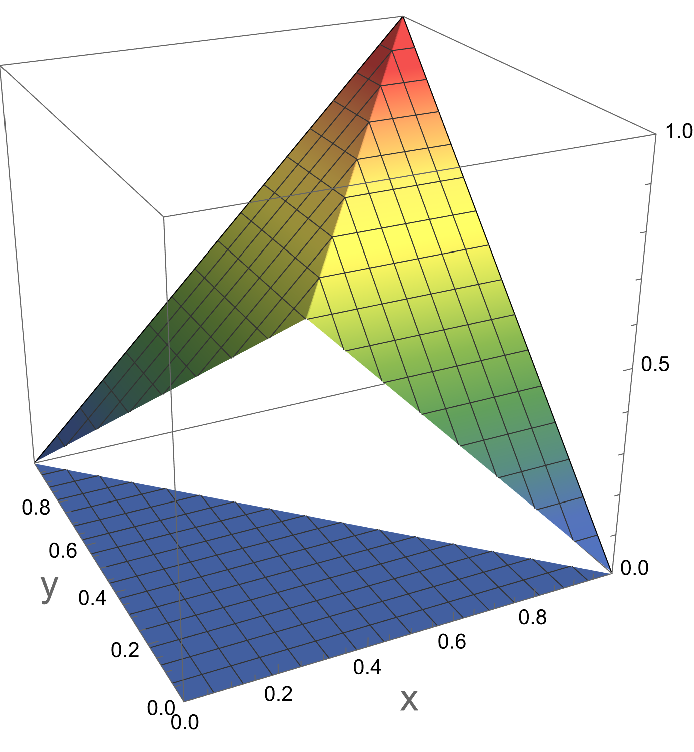
\includegraphics[scale=0.35]{TNM.pdf}
	\caption{$T_{\bm nM}$}
	\end{subfigure}
	\caption{Plots of basic t-norms presented in Table \ref{table:basic_tnorms}.}\label{fig:basic_tnorms}
\end{figure}

\begin{figure}[ht!]
	\centering
	\begin{subfigure}{.3\textwidth}
		\centering
		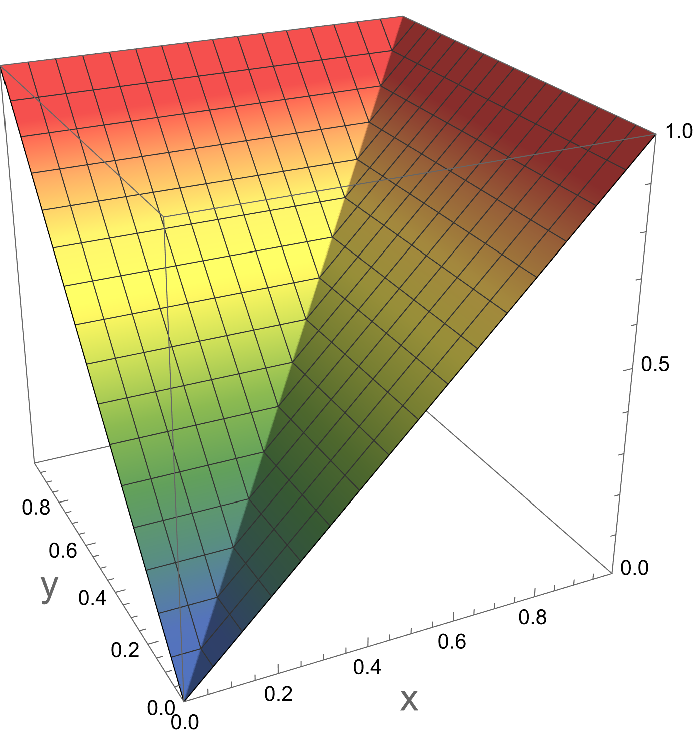
\includegraphics[scale=0.35]{SM.pdf}
		\caption{$S_{\bm M}$}
	\end{subfigure}\hspace{0.5cm}
	\begin{subfigure}{.3\textwidth}
		\centering
		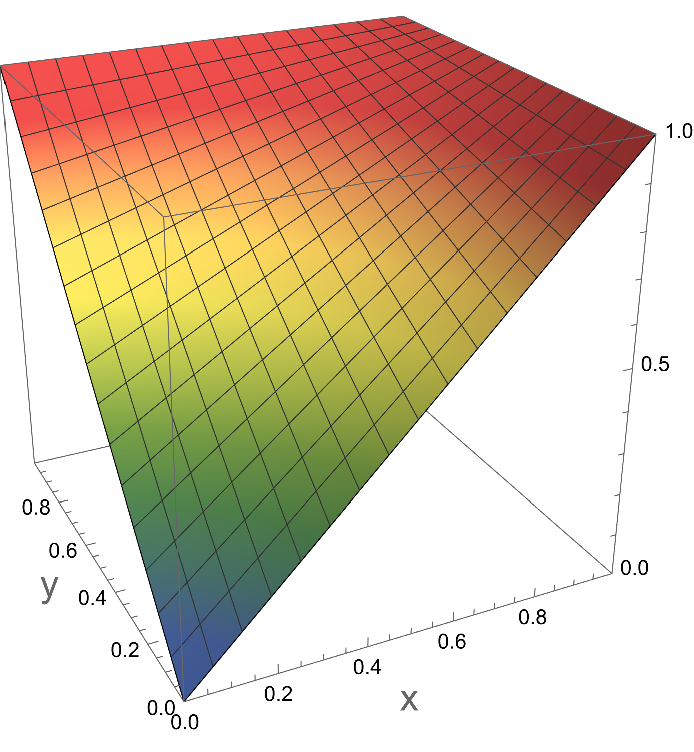
\includegraphics[scale=0.35]{SP.pdf}
		\caption{$S_{\bm P}$}
	\end{subfigure}\hspace{0.5cm}
	\begin{subfigure}{.3\textwidth}
		\centering
		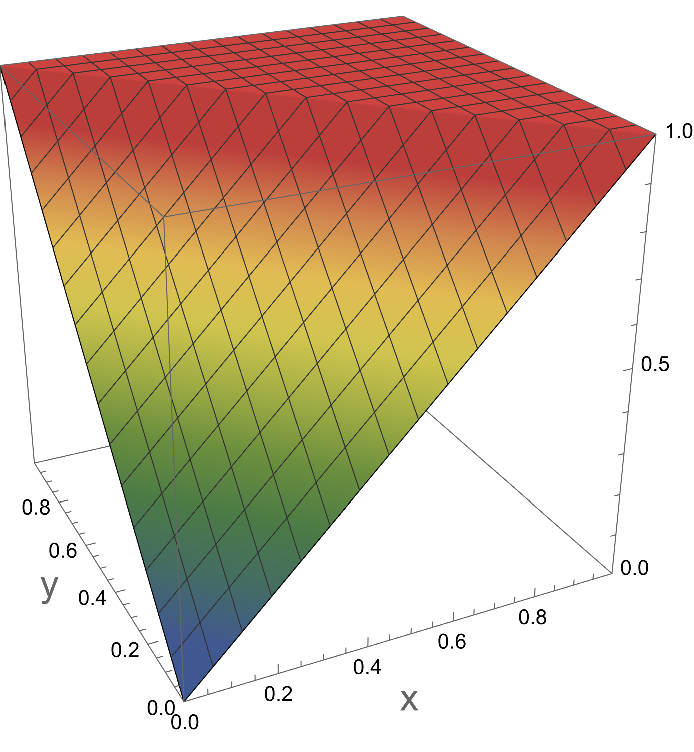
\includegraphics[scale=0.35]{SLK.pdf}
		\caption{$S_{\bm LK}$}
	\end{subfigure}\\
	\hspace{0.25cm}
	\begin{subfigure}{.4\textwidth}
		\centering
		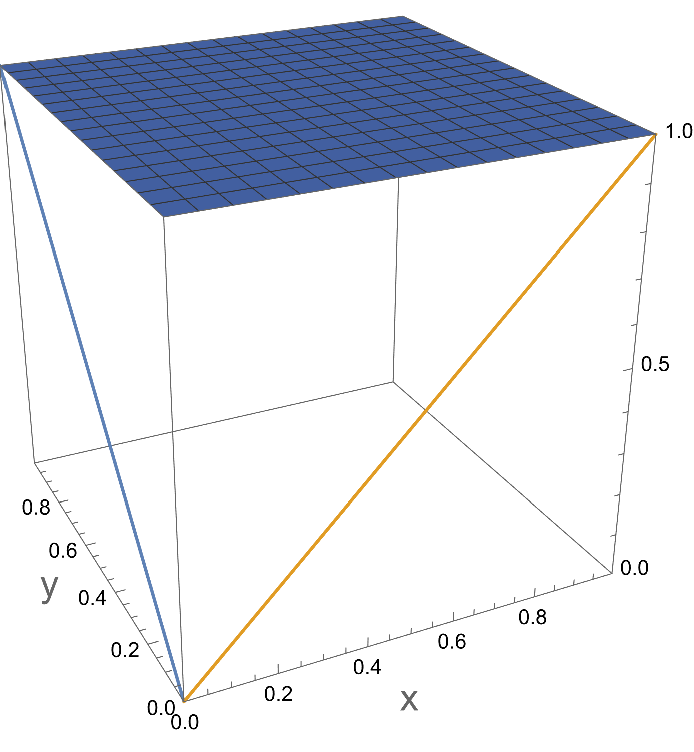
\includegraphics[scale=0.35]{SD.pdf}
		\caption{$S_{\bm D}$}
	\end{subfigure}\hspace{0.25cm}
	\begin{subfigure}{.4\textwidth}
		\centering
		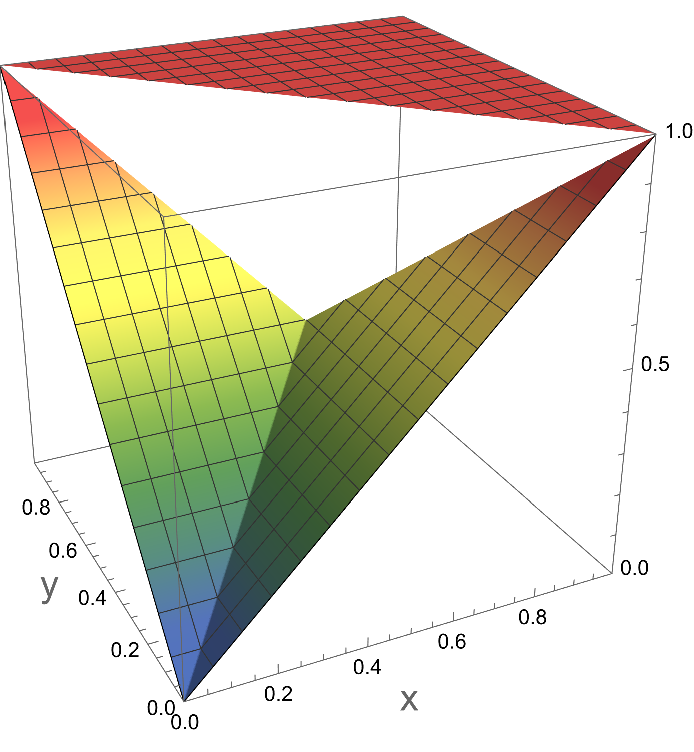
\includegraphics[scale=0.35]{SNM.pdf}
		\caption{$S_{\bm nM}$}
	\end{subfigure}
	\caption{Plots of basic t-conorms presented in Table \ref{table:basic_toconorms}.}\label{fig:basic_tconorms}
\end{figure}

Hereafter, we name several subclasses of t-norms and t-conorms.

\begin{definition}[\bf{\cite[Definition 2.1.2]{Baczynski2008}}] A t-norm $T:[0,1]^2 \to [0,1]$ is called
	\begin{itemize}
		\item \emph{idempotent} if $T(x,x)=x$ for all $x \in [0,1]$;
		\item \emph{positive} if $T(x,y)=0$ implies either $x=0$ or $y=0$;
		\item \emph{cancellative} if $T(x,y)=T(x,z)$ implies $y=z$ for all $x,y,z \in [0,1]$, $x>0$;
		\item \emph{conditionally cancellative} if $T(x,y)=T(x,z)>0$ implies $y=z$ for all $x,y,z \in [0,1]$;
		\item \emph{Archimedean} if for all $x,y \in (0,1)$ there exists an $n \in \NN$ such that $x_T^{(n)}<y$.
	\end{itemize}
\end{definition}

\begin{definition}[\textbf{\cite[Definition 2.13]{Klement2000}}]  A continuous Archimedean t-norm $T:[0,1]^2 \to [0,1]$ is called	
	\begin{itemize}
		\item \emph{strict} if it is strictly increasing on $(0,1]^2$.
		\item \emph{nilpotent} if there exists $(x,y) \in (0,1]^2$ such that $T(x,y)=0$.
	\end{itemize}
	A strict t-norm is cancellative and a nilpotent t-norm is conditionally cancellative.
\end{definition}

\pagebreak

\begin{definition}[\bf{\cite[Definition 2.2.2]{Baczynski2008}}] A t-conorm $S:[0,1]^2 \to [0,1]$ is called
	\begin{itemize}
		\item \emph{idempotent} if $S(x,x)=x$ for all $x \in [0,1]$;
		\item \emph{cancellative} if $S(x,y)=S(x,z)$ implies $y=z$ for all $x,y,z \in [0,1]$, $x<1$;
		\item \emph{conditionally cancellative} if $S(x,y)=S(x,z)<1$ implies $y=z$ for all $x,y,z \in [0,1]$;
		\item \emph{Archimedean} if for all $x,y \in (0,1)$ there exists an $n \in \NN$ such that $x_S^{(n)}>y$.
	\end{itemize}
\end{definition}

\begin{definition}[\textbf{\cite[Remark 2.20]{Klement2000}}]  A continuous Archimedean t-conorm $S:[0,1]^2 \to [0,1]$ is called	
	\begin{itemize}
		\item \emph{strict} if it is strictly increasing on $[0,1)^2$.
		\item \emph{nilpotent} if there exists $(x,y) \in [0,1)^2$ such that $S(x,y)=1$.
	\end{itemize}
	A strict t-conorm is cancellative and a nilpotent t-conorm is conditionally cancellative.
\end{definition}

It is well known that there exists a duality between t-norms and t-conorms which can be expressed in terms of a strictly decreasing bijection $\varphi:[0,1] \to [0,1]$ (see \cite[Proposition 2.34]{Klement2000}). In particular, this duality is usually considered in the case when $\varphi(x)=1-x$ for all $x \in [0,1]$.
\begin{proposition}[\bf{\cite[Proposition 2.2.3]{Baczynski2008}}]\label{prop:duality} For a function $S:[0,1]^2 \to [0,1]$, $S$ is a t-conorm if and only if there exists a t-norm $T:[0,1]^2 \to [0,1]$ such that 
	$$S(x,y)=1-T(1-x,1-y), \quad x,y \in [0,1].$$
	Moreover, the t-norm $T$ is continuous (Archimedean, cancellative, conditionally cancellative) if and only if the t-conorm $S$ is continuous (Archimedean, cancellative, conditionally cancellative).	
\end{proposition}


For instance, each $S_l$ in Figure $\ref{fig:basic_tconorms}$ is dual to $T_l$ in Figure \ref{fig:basic_tnorms} for all $l \in \{M,P,LK,D,nM\}$ in the sense of Proposition \ref{prop:duality}. Thanks to this duality, many results obtained for t-norms can be directly adapted for t-conorms.

Also, given a strong negation $N$ we can define the $N$-dual of a t-norm or a t-conorm, respectively.

\begin{proposition}[\bf{\cite{Klement2000}}]\label{prop:N_dual} Let $N$ be a strong negation, the following statements hold:
	\begin{enumerate}[label=(\roman*)]
		\item For any t-norm $T:[0,1]^2 \to [0,1]$, the function $S: [0,1]^2 \to [0,1]$ defined by
		$$S(x,y)=N(T(N(x),N(y))), \quad x,y \in [0,1],$$
		is a t-conorm called the \emph{$N$-dual of $T$}.
		\item For any t-conorm $S:[0,1]^2 \to [0,1]$, the function $T: [0,1]^2 \to [0,1]$ defined by
		$$T(x,y)=N(S(N(x),N(y))), \quad x,y \in [0,1],$$
		is a t-norm called the \emph{$N$-dual of $S$}.
	\end{enumerate}
\end{proposition}

Consecutively, we give further results of continuous and Archimedean t-norms. Notice that a continuous t-norm is Archimedean if and only if it has only trivial idempotent points, i.e., 0 and 1.

For nilpotent t-norms it is interesting to consider their induced negation, since the points of the t-norm which are equal to zero can be described in terms of this function.

\begin{definition}[\textbf{\cite{Jenei1998}}]
	Let $T$ be a nilpotent t-norm, the \emph{induced negation} of $T$ is defined by
	$$N_T(x) = \max \{t \in [0,1] \mid T(x,t)=0\}, \quad \text{for all } x \in [0,1].$$
\end{definition}

\begin{proposition}[\textbf{\cite{Jenei1998}}]\label{prop:NTinvolutive}
	Let $T$ be a nilpotent t-norm, then $N_T$ is a strong fuzzy negation. Moreover,
	$$T(x,y)=0 \Leftrightarrow N_T(x) \geq y.$$
\end{proposition}

The structure of Archimedean t-norms can be described in terms of a continuous, strictly decreasing function that is unique up to a positive multiplicative constant.

\begin{theorem}[\textbf{\cite[Theorem 5.1]{Klement2000}}]\label{th:representation_archimedeantnorms}
	For a function $T:[0,1]^2 \to [0,1]$ the following statements are equivalent:
	\begin{enumerate}[label=(\roman*)]
		\item $T$ is a continuous Archimedean t-norm.
		\item $T$ has a continuous additive generator, i.e., there exists a continuous, strictly decreasing function $t:[0,1]\to [0,+\infty]$ with $t(1)=0$, which is uniquely determined up to a positive multiplicative constant, such that
		$$ T(x,y)=t^{(-1)}(t(x)+t(y)), \quad \text{for all } x,y \in [0,1],$$
		where $t^{(-1)}$ is the pseudo-inverse of $t$ given by $t^{(-1)}(x)=t^{-1}(\min\{t(0),x\})$ for all $x \in [0,+\infty]$.
	\end{enumerate}
\end{theorem}

Notice that from Theorem \ref{th:representation_archimedeantnorms} we deduce that the difference between a strict and a nilpotent Archimedean t-norm in terms of an additive generator is that the value $t(0)$ is infinite or not, respectively. In addition, the induced negation of a nilpotent t-norm can be expressed in terms of an additive generator.

\begin{remark}\label{remark:gen_negation}
	Let $T$ be a nilpotent t-norm, $N_T$ its induced negation and $t$ an additive generator of $T$. Then,
	$$N_T(x)=t^{-1}(t(0)-t(x)), \quad \text{for all } x \in [0,1].$$
\end{remark}

Moreover, from Theorem \ref{th:representation_archimedeantnorms} it can be derived that there is a duality between additive and multiplicative generators of continuous Archimedean t-norms.

\begin{remark}[\textbf{\cite[Remark 3.34]{Klement2000}}]
	Let $T$ be a continuous Archimedean t-norm and $t: [0,1] \to [0,+\infty]$ an additive generator of $T$. Then $\theta:[0,1] \to [0,1]$ defined by $\theta(x)=e^{-t(x)}$ for all $x \in [0,1]$ is a multiplicative generator of $T$, i.e., it is a strictly increasing function with $\theta(1)=1$ such that
	$$T(x,y)=\theta^{(-1)}(\theta(x)\cdot\theta(y)), \quad \text{for all } x,y \in [0,1].$$
\end{remark}

\begin{example}[\textbf{\cite{Klement2000}}]\label{ex:Lukasiewicz} The most well-known continuous Archimedean t-norms are the product t-norm \TP and the Łukasiewicz t-norm \TLK (see Table \ref{table:basic_tnorms} and Figure \ref{fig:basic_tnorms}). In fact, continuous Archimedean t-norms can be represented as the $\Phi$-conjugates of these two t-norms \cite[Propositions 5.9 and 5.10]{Klement2000}. The additive generators of \TP and \TLK are
$$t(x)=-k\ln(x), \quad t(x)=k(1-x),$$
for all $x \in [0,1]$ and $k>0$, respectively. Moreover, the induced negation of \TLK is $N_{\TLK}(x)=1-x$ for all $x \in [0,1]$.
\end{example}

Now, we recall the following proposition that contains two results about nilpotent t-norms that involve the induced negation and disclose some information about their structure. Since we have obtained these results from more general results of left-continuous t-norms we provide the explicit proof.

\begin{proposition}[\textbf{\cite{Jenei1998}}]
	\label{prop:PropertiesNT}
	Let $T$ be a nilpotent t-norm and $N_T$ its induced negation. The following statements hold:
	\begin{enumerate}[label=(\roman*)]
		\item Let $x \in (0,1]$ and $h_x : [N_T(x),1] \to [0,x]$ be the function defined by $h_x(y)=T(y,x)$. Then $h_x$ is continuous, strictly increasing and
		$$h_x^{-1}(z)=N_T(T(N_T(z),x)), \quad \text{for all } z \in [0,x].$$
		\item Let $x_1,x_2,y_1,y_2 \in [0,1]$. If $T(x_1,y_1)=T(x_2,y_2)>0$, then 
		$$T(N_T(x_1),y_2)=T(N_T(x_2),y_1).$$
	\end{enumerate}
\end{proposition}

\begin{proof}
	\begin{enumerate}[label=(\roman*)]
		\item Since a nilpotent t-norm is conditionally cancellative and due to Proposition \ref{prop:NTinvolutive} it is straightforward that $h_x$ is continuous and strictly increasing. Since $T$ is nilpotent, it is continuous and, in particular, is left-continuous and $N_T$ is a strong negation. Then by \cite[(i)-Theorem 2]{Jenei1998} for all $x \in (0,1]$ and $z \in[0,x]$ we have
		\begin{eqnarray*}
		N_T(T(x,N_T(z))) &=& \sup \{ t \in [0,1] \mid T(x,t) \leq z\} = \max \{t \in [0,1] \mid t \leq h_x^{-1}(z)\} \\
		&=& h_x^{-1}(z).
		\end{eqnarray*}
		\item Since $T(x_1,y_1), T(x_2,y_2)>0$ by Proposition \ref{prop:NTinvolutive} we have $N_T(x_1)<y_1$ and $N_T(x_2)<y_2$. Then by the fact that $N_T$ is involutive and by (i) we have
		$$h_{y_1}^{-1}(N_T(x_1))=N_T(T(x_1,y_1))=N_T(T(x_2,y_2))=h_{y_2}^{-1}(N_T(x_2)),$$
		and then
		\begin{eqnarray*}
			T(N_T(x_1),y_2) & = & T(T(h_{y_1}^{-1}(N_T(x_1)),y_1),y_2) = T(T(h_{y_1}^{-1}(N_T(x_1)),y_2),y_1) \\
			& = & T(T(h_{y_2}^{-1}(N_T(x_2)),y_2),y_1) = T(N_T(x_2),y_1).
		\end{eqnarray*}
	\end{enumerate}
\end{proof}

Another fact that reflects the importance of continuous Archimedean t-norms relies on the characterization of continuous t-norms, which states that a continuous t-norm can be described in terms of an ordinal sum of continuous Archimedean t-norms.

\begin{theorem}[\textbf{\cite[Theorem 5.11]{Klement2000}}]\label{th:characcontt-norm}
	For a function $T:[0,1]^2 \to [0,1]$ the following statements are equivalent:
	\begin{enumerate}[label=(\roman*)]
		\item $T$ is a continuous t-norm.
		\item $T$ is uniquely representable as an ordinal sum of continuous Archimedean t-norms, i.e., there exist a uniquely determined (finite or countably infinite) index set $A$, a family of uniquely determined pairwise disjoint open sub-intervals $\{(a_{\alpha},e_{\alpha})\}_{\alpha \in A}$ of $[0,1]$ and a family of uniquely determined continuous Archimedean t-norms $(T_{\alpha})_{\alpha \in A}$ such that
		$$T(x,y)
		=
		\left\{\begin{array}{ll}
			a_{\alpha}+(e_{\alpha}-a_{\alpha})\cdot T_{\alpha}\left(\frac{x-a_{\alpha}}{e_{\alpha}-a_{\alpha}},\frac{y-a_{\alpha}}{e_{\alpha}-a_{\alpha}}\right) & \text{if } x,y \in [a_{\alpha},e_{\alpha}), \\
			\min\{x,y\} & \text{otherwise.}
		\end{array}
		\right.
		$$
		In this case, we will write $T=(\langle a_{\alpha},e_{\alpha},T_{\alpha}\rangle)_{\alpha \in A}$.
	\end{enumerate}
\end{theorem}

% Powers of a t-norm
The powers of a t-norm $T$ generalize the notion of the diagonal (2nd power of a t-norm). In {\cite{Walker2002}} the $r$-th powers with respect to continuous t-norms are studied in detail, so we only include here  a brief description. From the associativity of any t-norm $T$, positive integer powers with respect to $T$ can be defined in the usual way (see Equation \ref{eq:powers:genF}), that is,
$$x_T^{(n)} = \overbrace{T(x,T(x,\dots,T(x,x)))}^{n \ times} = T(\overbrace{x,x,\ldots,x}^{n \ times}) \quad \text{for all} \  x\in[0,1], \ n\in \NN \text{ and } n\geq 2,$$
with the conventions $x_T^{(1)}=x$ and  $x_T^{(0)}=1$ for all $x \in [0,1]$.

Similarly, $n$-th roots and positive rational powers of an element $x \in [0,1]$ with respect to a t-norm $T$ are defined as
\[
x_T^{\left(\frac{1}{n}\right)}=\sup\{z \in [0,1] \ | \ z_T^{(n)}\leq x\}, \qquad  x_T^{\left(\frac{m}{n}\right)}=\left(x_T^{\left(\frac{1}{n}\right)}\right)_T^{(m)},
\]
for all $m,n \in \NN$.

\begin{lemma}[\bf{\cite{Walker2002}}]
	\label{fraccions equivalents}
	Consider $k,m,n \in \NN$ and let  $T$ be a continuous t-norm. Then $x_T^{\left(\frac{km}{kn}\right)}=x_T^{\left(\frac{m}{n}\right)}$ for all $x\in[0,1]$.
\end{lemma}

From the continuity of $T$, positive rational powers with respect to $T$ can be extended to positive irrational powers through the following definition. 

\begin{definition}[\bf{\cite{Walker2002}}]
	\label{potencies irracionals}
	Let $T$ be a continuous t-norm and $r$ a positive real number. Consider $\{a_n \}_{n\in \NN}$ a sequence of rational numbers such that $\displaystyle \lim_{n \to +\infty}a_n=r$. For all $x \in [0,1]$, the power $x_T^{(r)}$ is defined as
	\[
	x_T^{(r)}=\displaystyle \lim_{n \to +\infty}x_T^{(a_n)}.
	\]
	We can extend the definition to $r=+\infty$ in the same way and then
	\[
	x_T^{(+\infty)}=\displaystyle \lim_{n \to +\infty}x_T^{(a_n)},
	\]
	where $\{a_n \}_{n\in \NN}$ is a sequence of positive rational numbers such that $\displaystyle \lim_{n \to +\infty}a_n=+\infty$.
\end{definition} 

The continuity of $T$ ensures both, the existence of the limit and the independence of the considered sequence $\{a_n \}_{n\in \NN}$. It is immediate to check that $0\leq x_T^{(r)}\leq 1$ and $x_T^{(r)}\leq y_T^{(r)}$ whenever $x\leq y$ for all $x,y\in[0,1]$ and  $r\in [0,+\infty]$. 

When the selected t-norm is Archimedean, the $r$-th powers can be expressed in terms of an additive generator.

\begin{proposition}[\bf{\cite{Walker2002}}]
Let $T$ be a continuous Archimedean t-norm with additive generator $t$. Then,
$$x_T^{(r)}=t^{-1}(\min\{t(0),rt(x)\}), \quad \text{for all } x \in [0,1] \text{ and } r \in [0,+\infty],$$
with the convention that $+\infty \cdot 0 = 0$.
\end{proposition}


\subsection{Uninorms}
Uninorms are associative functions that were defined as a generalization of t-norms and t-conorms \cite{Yager1996} by allowing any element $e \in [0,1]$ to act as a neutral element.

\begin{definition}[\bf{\cite{Yager1996,Klement2000}}]\label{def:uninorm}
	A binary operator $U:[0,1]^2 \to [0,1]$ is said to be a \emph{uninorm} if there exists $e \in [0,1]$, called \emph{neutral element}, such that $U$ satisfies:
	\begin{description}
		\item[(U1)] $U(x,y)=U(y,x)$ for all $x,y \in [0,1]$. \hfill (Commutativity)
		\item[(U2)] $U(x,U(y,z))=U(U(x,y),z)$ for all $x,y,z \in [0,1]$. \hfill (Associativity)
		\item[(U3)] $U(x,y) \leq U(x,z)$ when $y \leq z$, for all $x,y,z \in [0,1]$. \hfill (Monotonicity)
		\item[(U4)] $U(x,e)=x$ for all $x \in [0,1]$. \hfill (Neutral element)
	\end{description}
\end{definition}

From Definition \ref{def:uninorm} it is clear that $U$ is a t-norm if $e=1$ and a t-conorm if $e=0$. Thus, in order to distinguish these operators from these particular cases we say that a uninorm is \emph{proper} if $e \in (0,1)$. Besides, it holds that $U(1,0) \in \{0,1\}$ and we say that $U$ is \emph{conjunctive} if $U(1,0)=0$ and \emph{disjunctive} if $U(1,0)=1$.

The structure of uninorms is more complex than t-norms and t-conorms, so usually these operators are classified in different families \cite{Mas2015}. Some well-known characterized families of uninorms can be found hereunder.

\subsubsection{Uninorms in $\mathcal{U}_{\min}$ and $\mathcal{U}_{\max}$}

\begin{theorem}[\textbf{\cite[Theorem 1]{Mas2015}}]
	Let $U$ be a uninorm with neutral element $e \in (0,1)$.
	\begin{enumerate}[label=(\roman*)]
		\item If $U(0,1)=0$ and the function $U(\cdot,1)$ is continuous except in $x=e$, then $U$ is given by
		\begin{equation}\label{eq:umin}
			U(x,y)
			=
			\left\{\begin{array}{ll}
				e \cdot T_U\left(\frac{x}{e},\frac{y}{e}\right) & \text{if } x,y \in [0,e], \\
				e + (1-e) \cdot S_U\left(\frac{x-e}{1-e},\frac{y-e}{1-e}\right) & \text{if } x,y \in [e,1], \\
				\min\{x,y\} & \text{otherwise.}
			\end{array}
			\right.
		\end{equation}
		\item If $U(0,1)=1$ and the function $U(\cdot,0)$ is continuous except in $x=e$, then $U$ is given by
		\begin{equation}\label{eq:umax}
			U(x,y)
			=
			\left\{\begin{array}{ll}
				e \cdot T_U\left(\frac{x}{e},\frac{y}{e}\right) & \text{if } x,y \in [0,e], \\
				e + (1-e) \cdot S_U\left(\frac{x-e}{1-e},\frac{y-e}{1-e}\right) & \text{if } x,y \in [e,1], \\
				\max\{x,y\} & \text{otherwise.}
			\end{array}
			\right.
		\end{equation}
	\end{enumerate}
	In both formulas $T_U$ is a t-norm and $S_U$ is a t-conorm. The class of uninorms of the form (\ref{eq:umin}) is denoted by $\mathcal{U}_{\min}$, while the class of uninorms of the form (\ref{eq:umax}) is denoted by $\mathcal{U}_{\max}$.
\end{theorem}

\subsubsection{Idempotent uninorms}

\begin{definition}[\textbf{\cite[Definition 5.1.5]{Baczynski2008}}]
	A uninorm $U$ such that $U(x,x)=x$ for all $x \in [0,1]$ is said to be an \emph{idempotent uninorm}. The class of all idempotent uninorms is denoted by $\mathcal{U}_{Idem}$.
\end{definition}

\begin{theorem}[\textbf{\cite[Theorem 5]{Mas2015}}]
	For a function $U : [0,1]^2 \to [0,1]$ the following statements are equivalent:
	\begin{enumerate}[label=(\roman*)]
		\item $U$ is an idempotent uninorm with neutral element $e \in [0,1]$.
		\item There exists a decreasing function $g: [0,1] \to [0,1]$, symmetric with respect to the main diagonal, with $g(e)=e$, such that
		\begin{equation}\label{eq:uidempotent}
			U(x,y)
			=
			\left\{\begin{array}{ll}
				\min\{x,y\} & \text{if } y<g(x) \text{ or } (y=g(x) \text{ and } x<g(g(x))), \\
				\max\{x,y\} & \text{if } y>g(x) \text{ or } (y=g(x) \text{ and } x>g(g(x))), \\
				x \text{ or } y & \text{if } y=g(x) \text{ and } x=g(g(x)), \\
			\end{array}
			\right.
		\end{equation}
	being commutative in the points $(x,y)$ such that $y=g(x)$ with $x=g(g(x))$.
	\end{enumerate}
\end{theorem}

%\begin{center}
%	\textsc{Representable Uninorms}
%\end{center}

\subsubsection{Representable uninorms}

\begin{definition}[\textbf{\cite[Theorem 5.1.12]{Baczynski2008}}]
	A uninorm $U$ is called \emph{representable} if it has a continuous additive generator, i.e., there exists a continuous and strictly increasing function $h:[0,1] \to [-\infty,+\infty]$ such that $h(0)=-\infty$, $h(e)=0$ for an $e \in (0,1)$ and $h(1)=+\infty$, which is uniquely determined up to a positive multiplicative constant, such that
	$$U(x,y)
	=
	\left\{\begin{array}{ll}
		0 & \text{if } (x,y) \in \{(0,1),(1,0)\}, \\
		h^{-1}(h(x)+h(y)) & \text{otherwise},
	\end{array}
	\right.
	$$
	or 
	$$U(x,y)
	=
	\left\{\begin{array}{ll}
		1 & \text{if } (x,y) \in \{(0,1),(1,0)\}, \\
		h^{-1}(h(x)+h(y)) & \text{otherwise}.
	\end{array}
	\right.
	$$
	The class of all representable uninorms is denoted by  $\mathcal{U}_{Rep}$.
\end{definition}

For more details regarding uninorms we refer the reader to \cite{Mas2015} and references therein.

\subsection{Copulas}

Copulas are binary operators $C:[0,1]^2 \to [0,1]$ that were originated in the context of statistics and play a major role in Sklar's theorem, which states that any two-dimensional distribution function can be written in terms of two marginal distribution functions and a copula, which describes the dependence between the variables \cite{Sklar1959,Nelsen1999}. However, copulas are also studied as fuzzy conjunctions which, unlike t-norms, are not necessarily commutative or associative.
\begin{definition}[\textbf{\cite[Definition 2.2.2]{Nelsen1999}}]
	A \emph{copula} is a function $C: [0,1]^2 \to [0,1]$ which satisfies the following conditions:
	\begin{enumerate}[label=(\roman*)]
		\item $C(x,0)=C(0,y)=0$ for all $x,y \in [0,1]$.
		\item $C(x,1)=x$ for all $x \in [0,1]$.
		\item $C(1,y)=y$ for all $y \in [0,1]$.
		\item Let, $x_1,x_2,y_1,y_2 \in [0,1]$ such that $x_1 \leq x_2$ and $y_1 \leq y_2$, then
		$$C(x_2,y_2)-C(x_2,y_1)-C(x_1,y_2)+C(x_1,y_1) \geq 0.$$
	\end{enumerate}
\end{definition}

\begin{example}
There exist many different families of copulas but, according to \cite{Sriboonchitta2018} the Farlie-Gumbel-Morgenstern (FGM) copula is one of the most important:
$$C(x,y)=x \cdot y + \theta \cdot x \cdot (1-x) \cdot y \cdot (1-y),$$
for all $x,y \in [0,1]$ and $\theta \in [-1,1]$.
\end{example}

For more details regarding copulas and other related operators we refer the reader to \cite{Nelsen1999,Beliakov2010,Calvo2002,Grabisch2009}.


\section{Fuzzy implication functions}\label{section:fuzzy_implication_functions}

Similarly to fuzzy negations, t-norms or t-conorms, fuzzy implication functions are a generalization of the corresponding classical operator to fuzzy logic. In this section we give the definition of a fuzzy implication function, we recall some of their main additional properties and we provide several examples. Also, we present the families that are related to the results of this monograph.

\subsection{Definition and additional properties}\label{subsection:definition&additionalproperties}
The most accepted definition of fuzzy implication functions is the following one.
\begin{definition}[\bf{\cite{Baczynski2008,Fodor1994}}]\label{defimp}
	A binary operator $I:[0,1]^2 \to [0,1]$ is said to be a \emph{fuzzy implication function} if it satisfies:
	\begin{description}
		\item[\Ione]  $I(x,z)\geq I(y,z)\ $  when  $\ x\leq y$, for all $x,y,z\in[0,1]$. \hfill (Left Antitonicity)
		\item[\Itwo]  $I(x,y)\leq I(x,z)\ $  when  $\ y\leq z$, for all $x,y,z\in[0,1]$. \hfill (Right Isotonicity)
		\item[\Ithree]  $I(0,0)=I(1,1)=1$ and $I(1,0)=0$. \hfill (Boundary Condition)
	\end{description}
\end{definition}
If we recall the truth table of the classical implication
\begin{center}
	\begin{tabular}{|c|c|c|}
		\hline
		$p$ & $q$ & $p \to q$ \\ \hline
		0   & 0   & 1         \\ \hline
		0   & 1   & 1         \\ \hline
		1   & 0   & 0         \\ \hline
		1   & 1   & 1         \\ \hline
	\end{tabular}
\end{center}
\noindent it is clear that the boundary condition \Ithree ensures that a fuzzy implication function restricted to $\{0,1\}^2$ coincides with the classical implication (note that $I(0,1)=1$ is guaranteed due to $I(0,0)=1$ and \Itwo. In addition, \Ione incorporates the idea that a lower truth value of the first variable is more efficient to state more about the truth value of its consequent. On the other hand, \Itwo is connected to the idea that the overall truth value depends on the consequent directly.

From Definition \ref{defimp} it can be easily derived that $I(0,x) = I(x,1) = 1$ for all $x \in [0, 1]$. However, the values $I(x,0)$ and $I(1,x)$ are not predetermined by the definition. In fact, the values $I(x,0)$ define what is called the natural negation of a fuzzy implication function.
\begin{definition}[\textbf{\cite[Definition 1.4.14]{Baczynski2008}}]\label{def:naturalnegationI}
	Let $I$ be a fuzzy implication function. The function $N_I:[0,1] \to [0,1]$ defined by
	$$N_I(x)=I(x,0), \quad \text{for all } x \in [0,1],$$
	is a fuzzy negation called the \emph{natural negation} of $I$.
\end{definition}

\begin{remark}
	For the sake of simplicity, some results related to the characterization of fuzzy implication functions use the notation $N_I$ where $I:[0,1]^2 \to [0,1]$ is an arbitrary binary function. When $I$ is not a fuzzy implication function this notation refers to the horizontal section $I(\cdot,0)$, which may not be a fuzzy negation.
\end{remark}

Since Definition \ref{defimp} is quite general, additional properties of these operators are usually considered. These properties come often in the form of functional equations which involve fuzzy implication functions and some of them, other operators as well. The motivation behind the definition of these additional properties are diverse, but the most usual are: a large majority of them were introduced as the straightforward generalizations of classical logic tautologies to fuzzy logic; others point out some desirable or interesting analytical/algebraic properties of these functions; some were introduced since they appeared when solving a particular problem; finally, many of these properties aim to be useful in a particular problem or application. Since a lot of additional properties have been introduced in the literature, we limit ourselves to list here the most popular and the ones that are relevant to the results presented in this monograph.

\begin{itemize}
	\item The \emph{left neutrality principle}
	$$I(1,y)=y, \quad y\in[0,1]. \eqno {\text{\NP}}$$
	\item The \emph{exchange principle} 
	$$I(x,I(y,z)) = I(y,I(x,z)), \quad  x,y,z\in[0,1]. \eqno {\text{\EP}}$$
	\item The \emph{identity principle} 
	$$ I(x,x)=1, \quad x\in[0,1]. \eqno {\text{\IP}}$$
	\item The \emph{ordering property} 
	$$I(x,y)=1 \Leftrightarrow x \leq y, \quad x,y\in[0,1]. \eqno {\text{\OP}}$$
	\item The \emph{consequent boundary}
	$$ I(x,y)\geq y, \quad x,y \in [0,1]. \eqno {\text{\CB}}$$
	\item The \emph{iterative boolean law}
	$$ I(x,y)=I(x,I(x,y)), \quad x,y \in [0,1]. \eqno {\text{\IB}}$$
	\item The \emph{lowest falsity property}
	$$ I(x,y)=0 \Leftrightarrow x=1 \text{ and } y=0. \eqno {\text{\LF}}$$
	\item The \emph{lowest truth property}
	$$ I(x,y)=1 \Leftrightarrow x=0 \text{ or } y=1. \eqno {\text{\LT}}$$
	\item The \emph{contrapositive symmetry} with respect to a fuzzy negation $N$
	$$ I(x,y)=I(N(y),N(x)), \quad x,y \in [0,1]. \eqno {\text{\CPN}}$$
	\item The \emph{law of left contraposition} with respect to a fuzzy negation $N$
	$$ I(N(x),y)=I(N(y),x), \quad x,y \in [0,1]. \eqno {\text{\LCP}}$$
	\item The \emph{law of right contraposition} with respect to a fuzzy negation $N$
	$$ I(x,N(y))=I(y,N(x)), \quad x,y \in [0,1]. \eqno {\text{\RCPN}}$$
	\item The \emph{law of importation} with respect to a t-norm $T$ 
	$$I(T(x,y),z) = I(x,I(y,z)), \quad  x,y,z\in[0,1]. \eqno {\text{\LI}}$$
	\item The \emph{left neutrality principle with $e\in (0,1) $}
	$$I(e,y)=y, \quad y\in[0,1]. \eqno {\text{\NPe}}$$
	\item  The \emph{$T$-conditionality} with respect to a t-norm $T$
	$$ T(x,I(x,y)) \leq y, \quad x,y \in [0,1]. \eqno {\text{\TC}}$$
	\item The \emph{distributivity laws} with respect to a t-norm $T$ and a t-conorm $S$
	$$I(S(x,y),z)=T(I(x,z),I(y,z)), \quad x,y,z \in [0,1]. \eqno {\text{\DST}}$$
	$$I(T(x,y),z)=S(I(x,z),I(y,z)), \quad x,y,z \in [0,1]. \eqno {\text{\DTS}}$$
	$$I(x,T(y,z))=T(I(x,y),I(x,z)), \quad x,y,z \in [0,1]. \eqno {\text{\DTT}}$$
	$$I(x,S(y,z))=S(I(x,y),I(x,z)), \quad x,y,z \in [0,1]. \eqno {\text{\DSS}}$$
		\item The \emph{$T$-power invariance} with respect to a continuous t-norm $T$
	$$I(x,y)=I\left(x_T^{(r)}, y_T^{(r)}\right), \eqno {\text{\PIT}}$$
	for all positive real numbers $r > 0$ and $x, y \in (0,1)$ such that $x_T^{(r)}, y_T^{(r)} \not = 0$.
\end{itemize}

\begin{remark}\label{remark:PITmodification}
	The definition of the $T$-power invariance with respect to a continuous t-norm $T$ considered in this thesis presents a slight modification with respect to the original one introduced in \cite{Massanet2017}. Specifically, the original definition (see \cite[Definition~5]{Massanet2017}) considers the equality \PIT on the points $x,y \in [0,1]$ such that $x_T^{(r)}, y_T^{(r)} \not = 0,1$, so it also takes into account the $T$-powers of zero. When assuming the original definition, one must take into account that when a non-strict t-norm $T$ is considered, it may happen that $0_T^{(r)}>0$ for some $r>0$. For instance if $T=\TLK$ then $0_{\TLK}^{0.5}=0.5$. Nonetheless, in \cite{Massanet2017} and subsequent papers \cite{Massanet2019,Massanet2019B} the authors rule out the plausible case $x_T^{(r)} \not = 0$ or $y_T^{(r)} \not = 0$ with $x=0$ or $y=0$ in some proofs (see for instance \cite[Propositions 11 and 12]{Massanet2019B}). In view of this situation, we have chosen to modify the corresponding definition to suit the way in which the authors have interpreted it in the results, i.e., discarding the evaluation of the equation $I(x,y)=I\left(x_T^{(r)}, y_T^{(r)}\right)$ when $x$, $y$, $x_T^{(r)}$ or $y_T^{(r)}$ are 0 or 1. This assumption results in the modified definition we have introduced above.  In this interpretation, the boundaries of the unit square are avoided on the two sides of the equation, and not only on the right side. It is clear that the two interpretations may lead to different results, but the comparison of the two perspectives has been considered beyond the scope of this thesis. Thus, throughout the report we consider the modified definition which is also the one used in the results in the existing literature \cite{Massanet2017,Massanet2019,Massanet2019B}.
\end{remark}

Many of these properties, which are not guaranteed by Definition \ref{defimp}, play a major role for a particular application. For instance:
\begin{itemize}
	\item The $T$-conditionality is required in approximate reasoning when the generalized modus ponens as inference mechanism is considered \cite{Baczynski2008}.
	\item  The law of importation \LI and the distributivity laws are useful for reducing the complexity of fuzzy inference mechanisms that involve fuzzy implication functions \cite{Combs1998,Jayaram2008,Jayaram2008B}. Besides, \LI is also considered for the definition of a fuzzy mathematical morphology with good algebraic properties \cite{Kerre2000}.
	\item The lowest falsity and lowest truth properties are needed for the construction of strong equality indices \cite{Bustince2013}.
	\item The ordering property \OP and the law of contraposition \CPN have been useful for constructing some measures from fuzzy implication functions employed in image processing \cite{Bustince2007,Bustince2008}.
	\item The invariance property \PIT, which is thoroughly studied in Chapter \ref{chapter:tpowerinvariant}, is derived from a potential demand in approximate reasoning when fuzzy implication functions are used to model fuzzy conditionals that involve linguistic modifiers \cite{Massanet2017}.
\end{itemize}

Apart from potential applications, the research on additional properties is of the utmost importance in the study of classes of fuzzy implication functions. Indeed, these properties aim to give a proper classification of fuzzy implication functions and to disclose the intersection between different classes. For instance, in Section \ref{subsection:families} the characterization of several families of fuzzy implication functions is recalled, and from these results, we can clearly see how some of these properties are the key of the characterization of the structure of the corresponding class. On the other hand, the study of additional properties can be generally considered as the study of different functional equations. The interrelationships between some of these properties are studied in \cite{Shi2010}.

In Table \ref{table:basic_implications} examples of fuzzy implication functions can be found. Moreover, in Figure \ref{fig:basic_implications} there is the plot of these examples.

\begin{table}[ht!]
	\centering
	\begin{tabular}{|C{3cm}|l|} \hline
		\bf Name & \multicolumn{1}{|c|}{\bf Formula} \\   
		\hline \bf {\L}ukasiewicz & $\ILK(x,y)=\min\{1,1-x+y\}$ \\
		\hline \bf Gödel & $\IGD(x,y)=\left\{\begin{array}{ll}1&\hbox{if } x\leq y\\y&\hbox{if } x>y\end{array}\right.$ \\
		\hline \bf Reichenbach & $\IRC(x,y)=1-x+xy$  \\
		\hline \bf Kleene-Dienes & $\IKD(x,y)=\max\{1-x,y\}$ \\
		\hline \bf Goguen & $\IGG(x,y)=\left \{\begin{array}{ll} 1& \hbox{if } x\leq y\\ \frac{y}{x}&\hbox{if } x>y\end{array}\right.$ \\
		\hline \bf Rescher & $\IRS(x,y)=\left \{\begin{array}{ll} 1& \hbox{if } x\leq y\\ 0&\hbox{if } x>y\end{array}\right.$ \\
		\hline \bf Yager & $\IYG(x,y)=\left \{\begin{array}{ll} 1& \hbox{if } x=0 \hbox{ and } y=0\\ y^x&\hbox{if } x>0 \hbox{ or } y>0\end{array}\right.$ \\
		\hline \bf Weber & $\IWB(x,y)=\left \{\begin{array}{ll} 1& \hbox{if } x<1\\ y&\hbox{if } x=1\end{array}\right.$  \\
		\hline \bf Fodor & $\IFD(x,y)=\left \{\begin{array}{ll} 1& \hbox{if } x\leq y\\ \max\{1-x,y\}&\hbox{if } x>y\end{array}\right.$  \\
		\hline \bf Least & $\ILT(x,y)=\left\{\begin{array}{ll} 1&\hbox{if } x=0 \hbox{ or } y=1\\ 0&\hbox{if } x>0 \hbox{ and } y<1 \end{array}\right.$ \\
		\hline \bf Greatest & $\IGT(x,y)=\left\{\begin{array}{ll} 1&\hbox{if } x<1 \hbox{ or } y>0\\ 0&\hbox{if } x=1 \hbox{ and } y=0 \end{array}\right.$ \\
		\hline
	\end{tabular}
	\caption{Basic Fuzzy Implication Functions.}\label{table:basic_implications}
\end{table}

\begin{figure}[htp!]
	\centering
	\subfloat[\ILK]{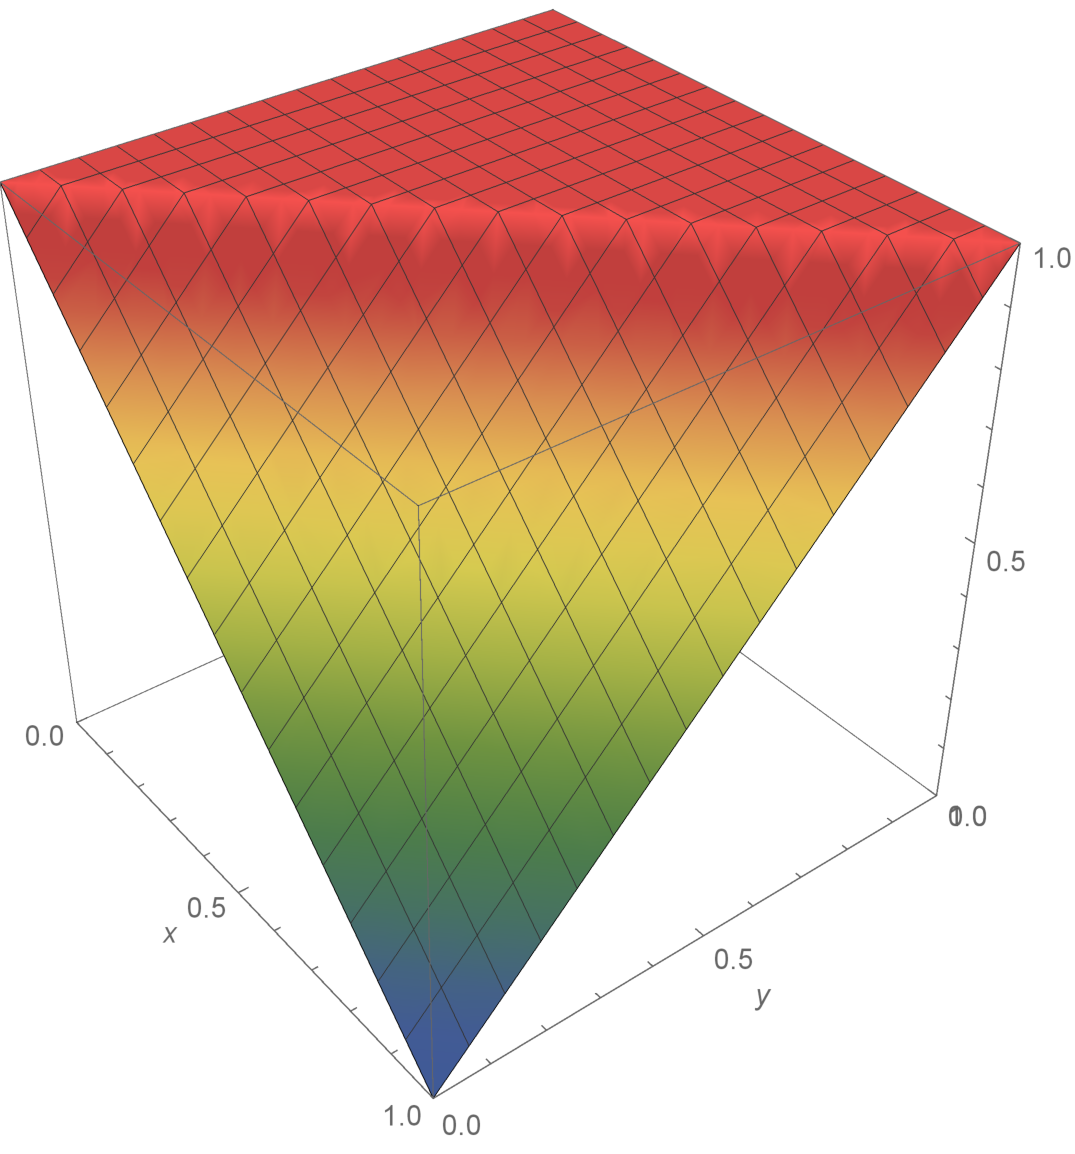
\includegraphics[width=4cm]{ILK.pdf} }
	\subfloat[\IGD]{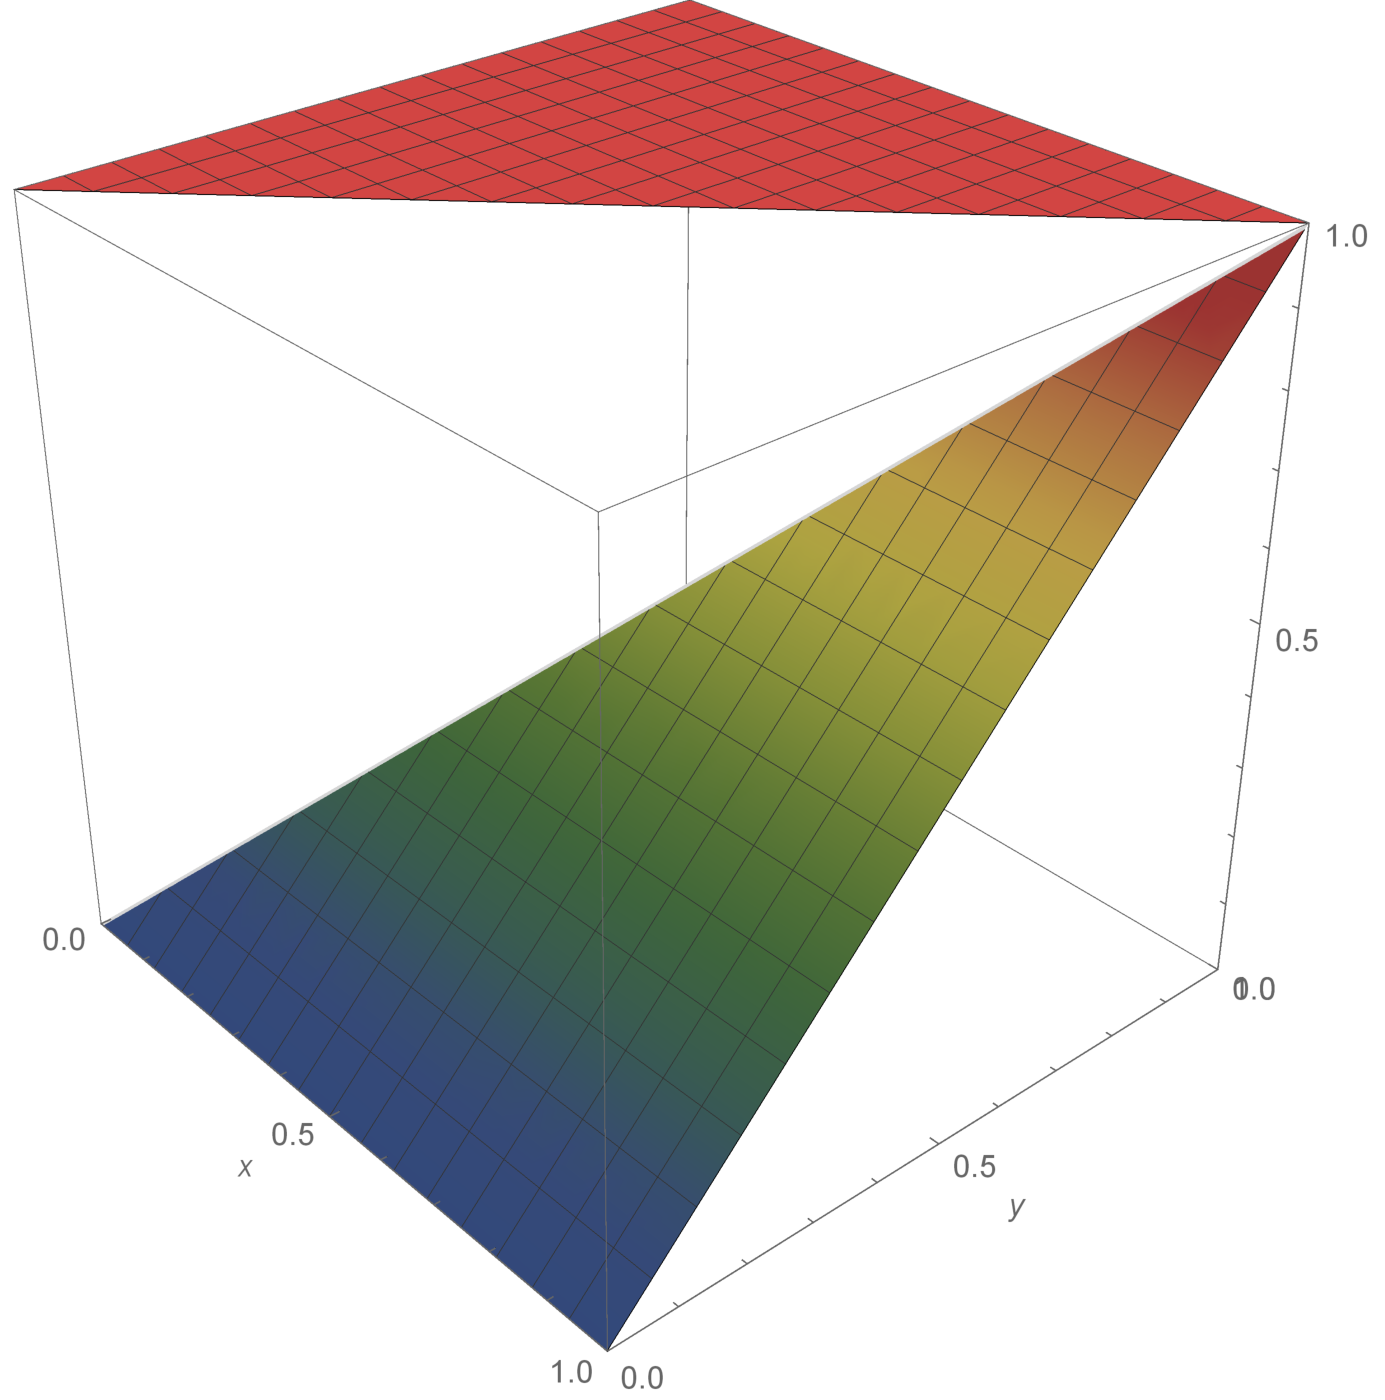
\includegraphics[width=4cm]{IGD.pdf} }
	\subfloat[\IRC]{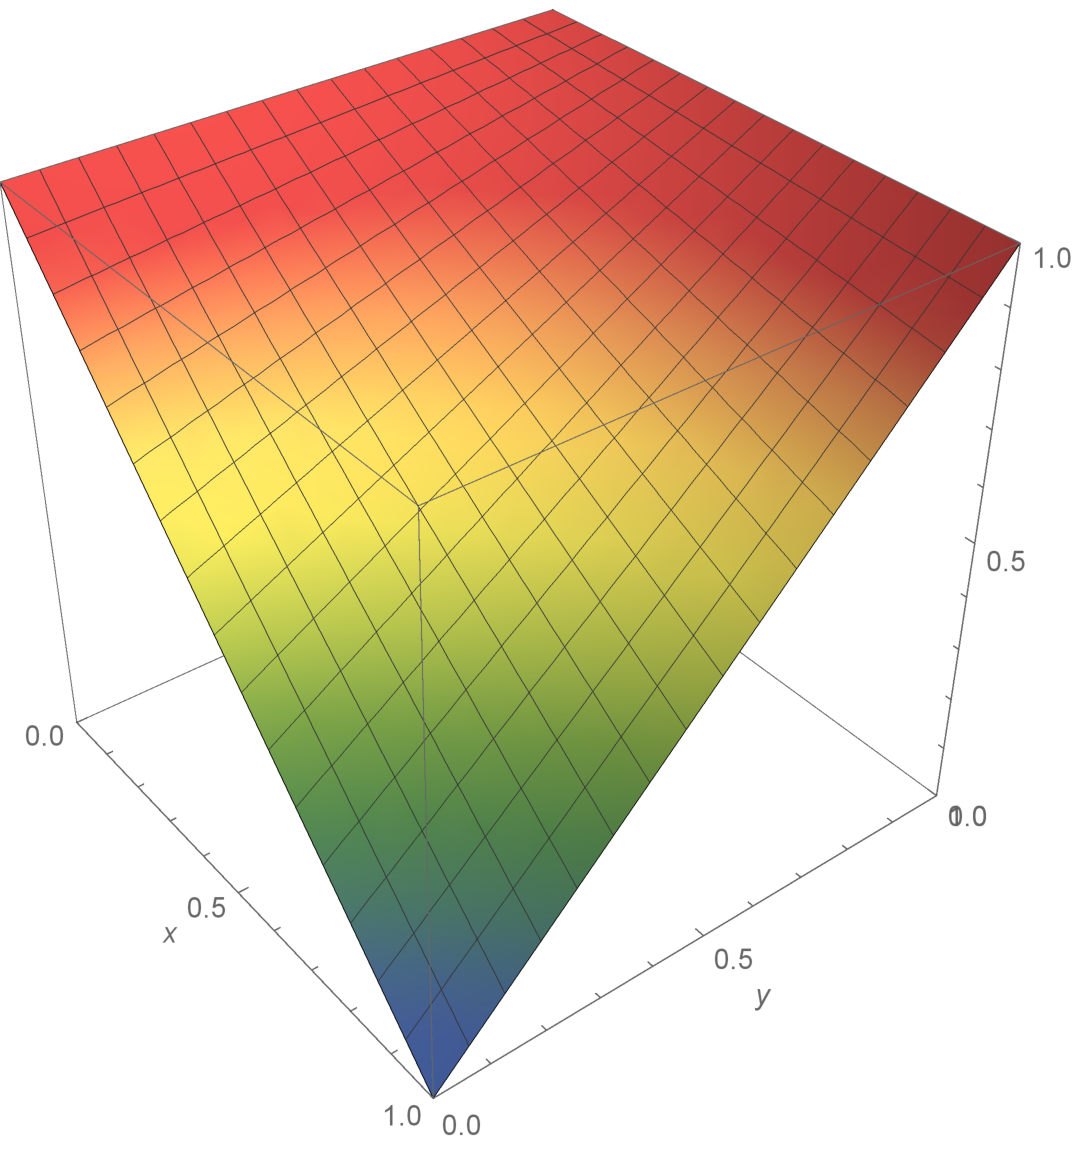
\includegraphics[width=4cm]{IRC.pdf} }\\
	\subfloat[\IKD]{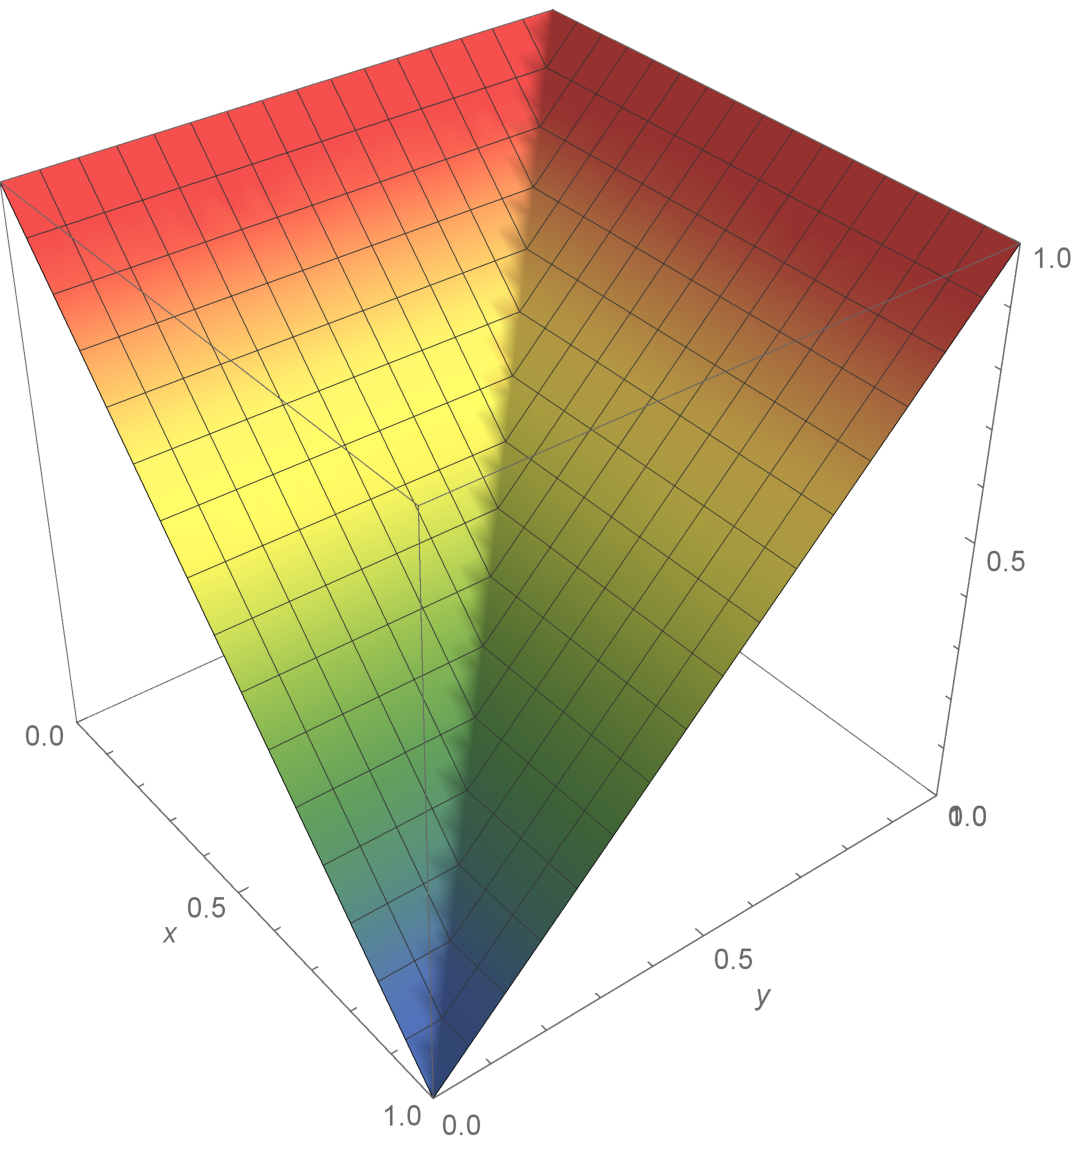
\includegraphics[width=4cm]{IKD.pdf} }
	\subfloat[\IGG]{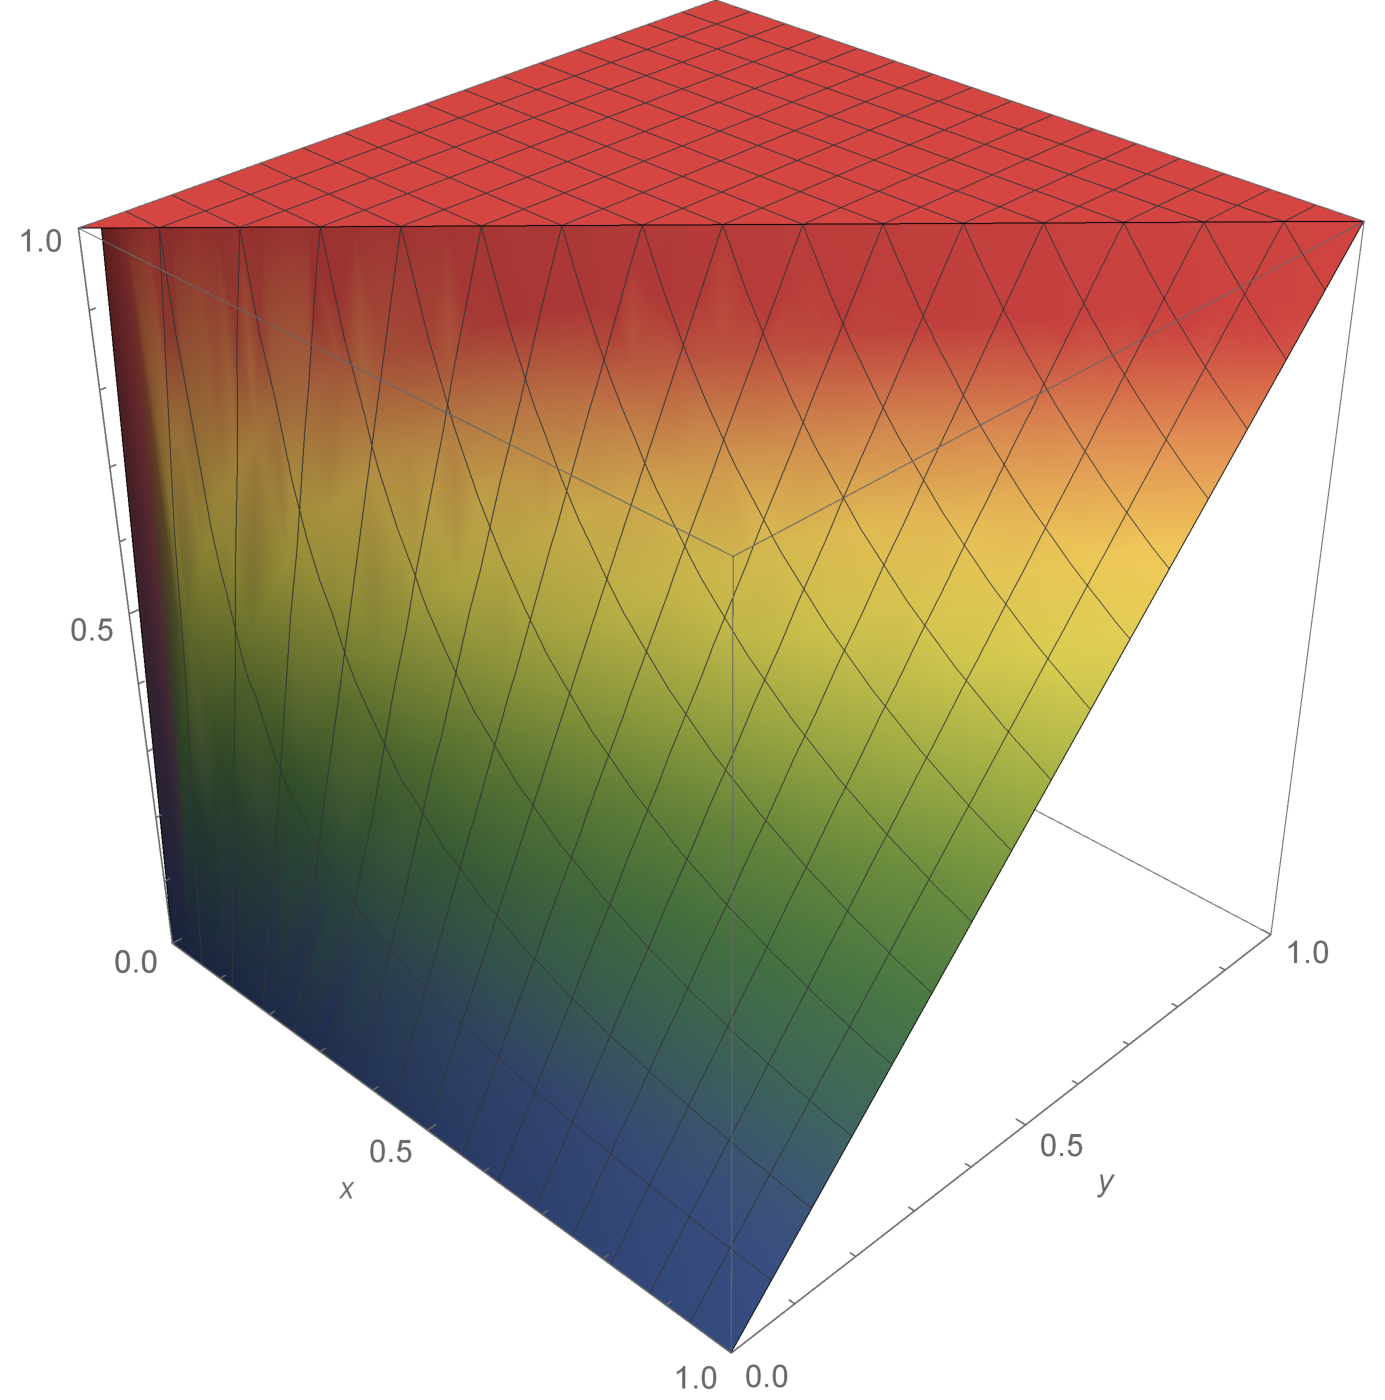
\includegraphics[width=4cm]{IGG.pdf} }
	\subfloat[\IRS]{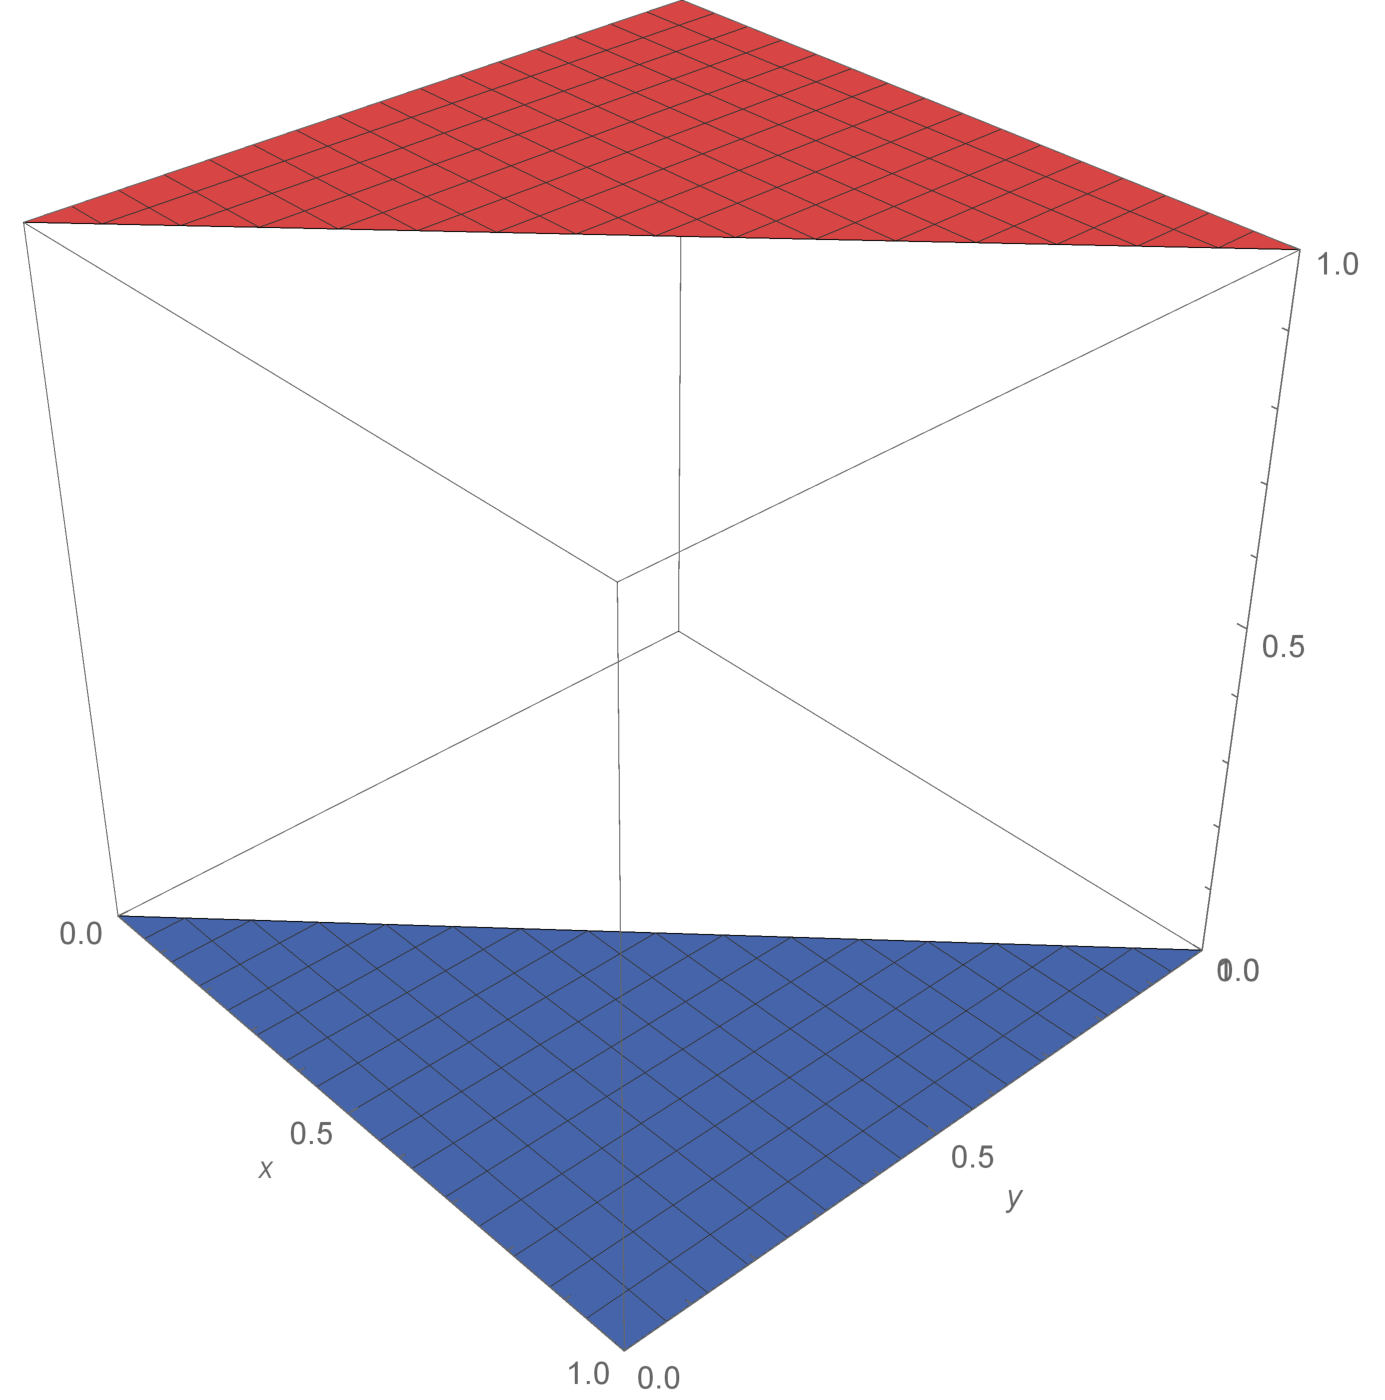
\includegraphics[width=4cm]{IRS.pdf} }\\
	\subfloat[\IYG]{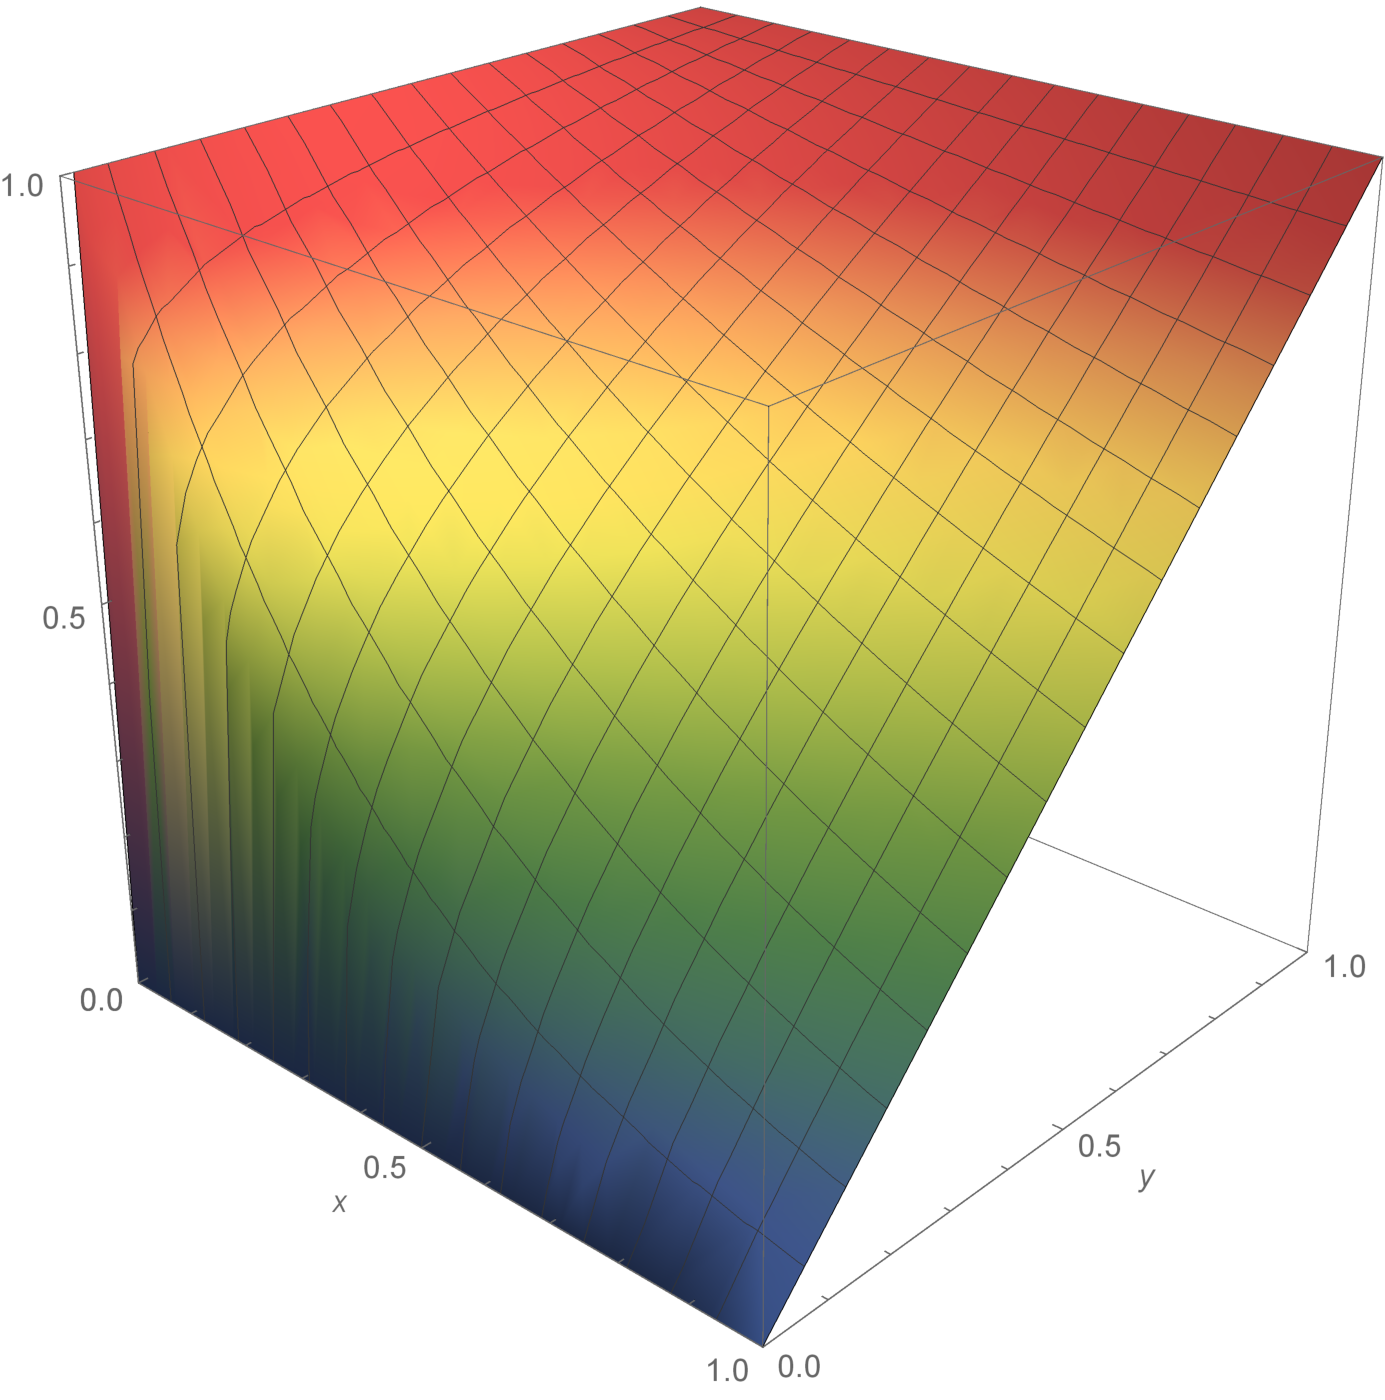
\includegraphics[width=4cm]{IYG.pdf} }
	\subfloat[\IWB]{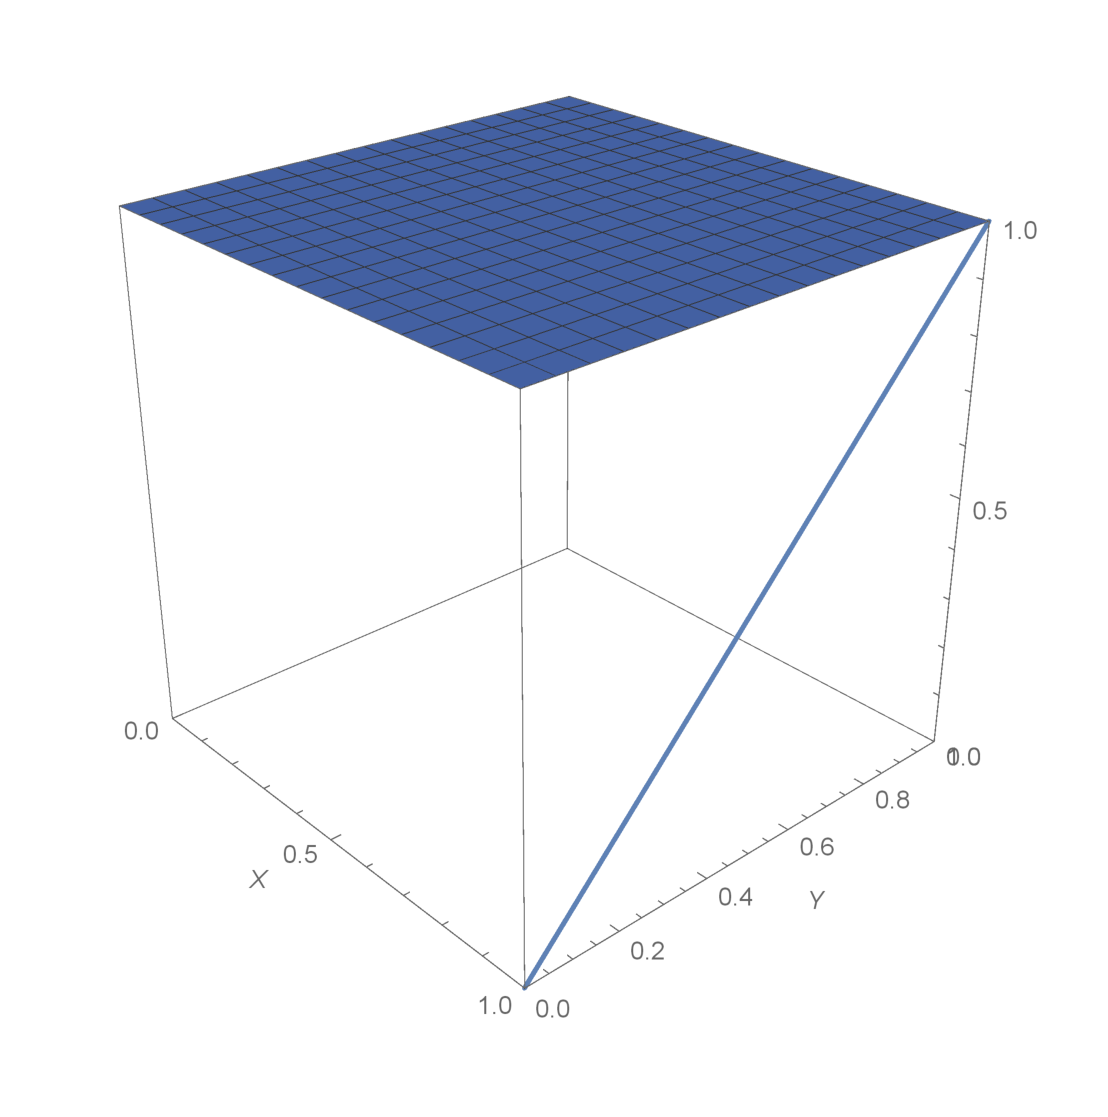
\includegraphics[width=4.5cm]{IWB.pdf} }
	\subfloat[\IFD]{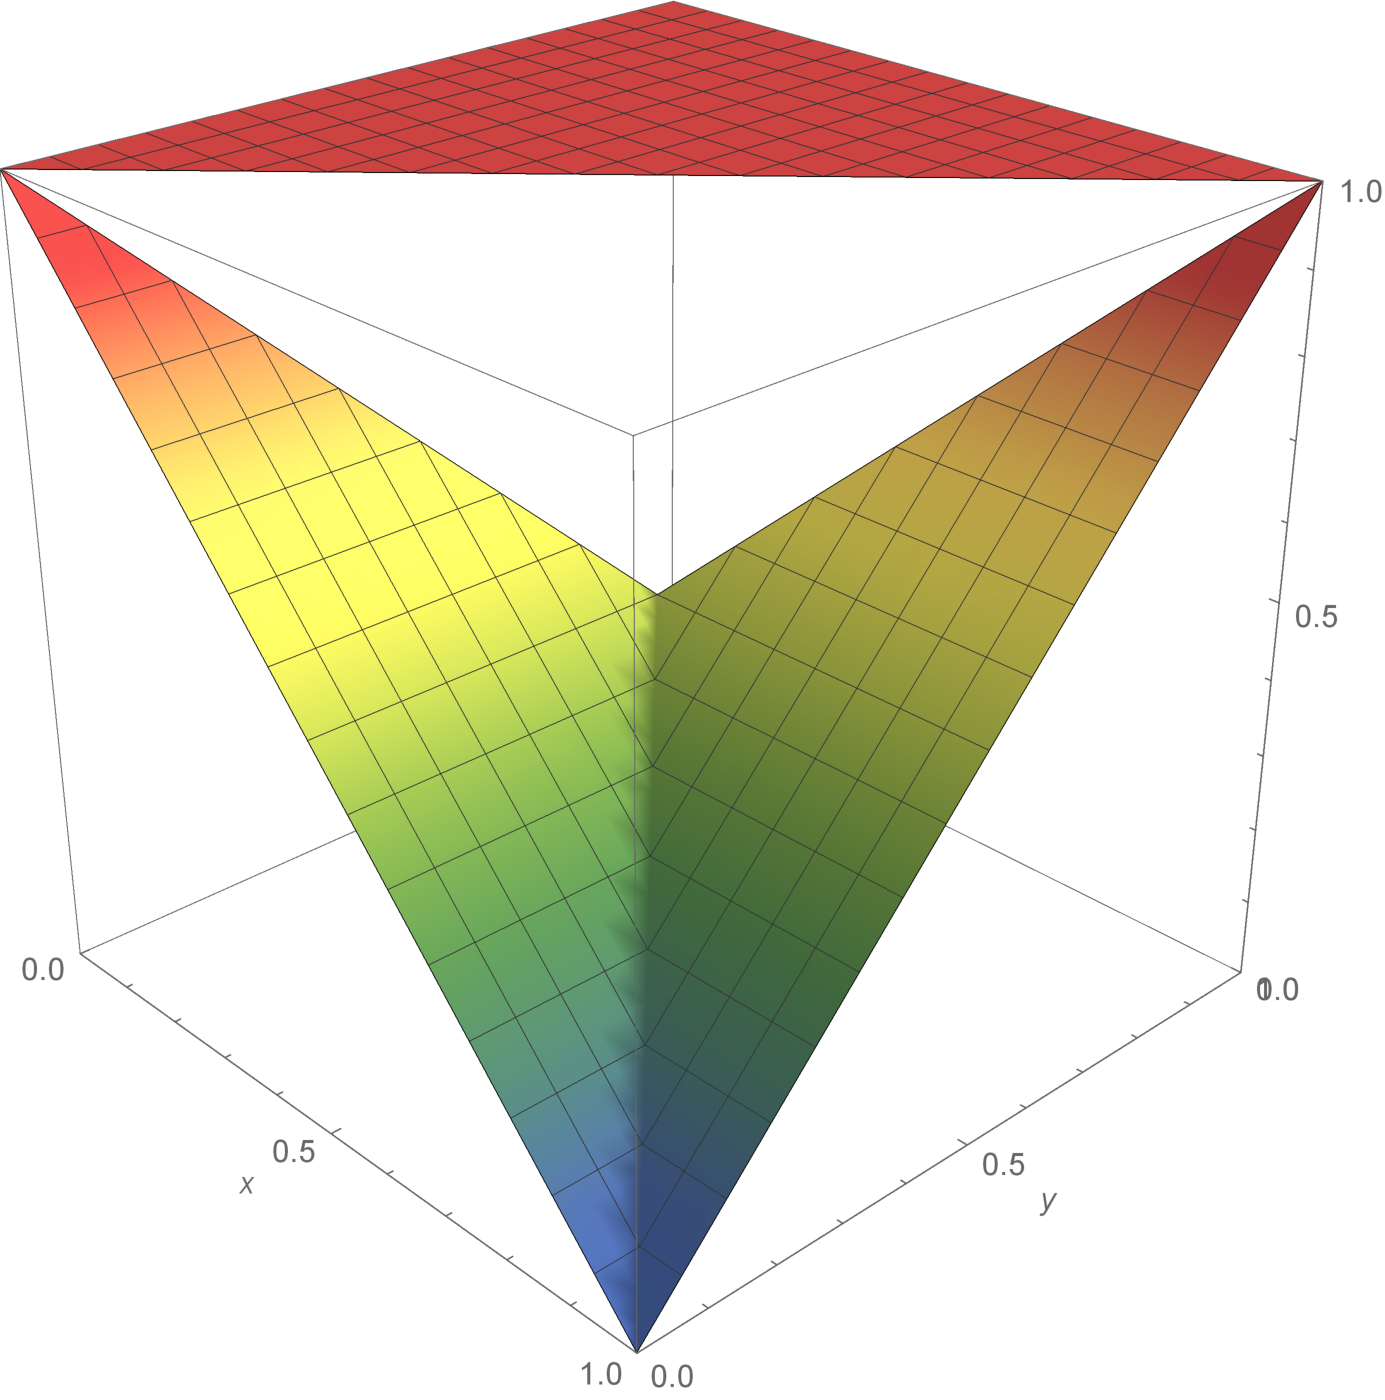
\includegraphics[width=4cm]{IFD.pdf} }\\
	\subfloat[\ILT]{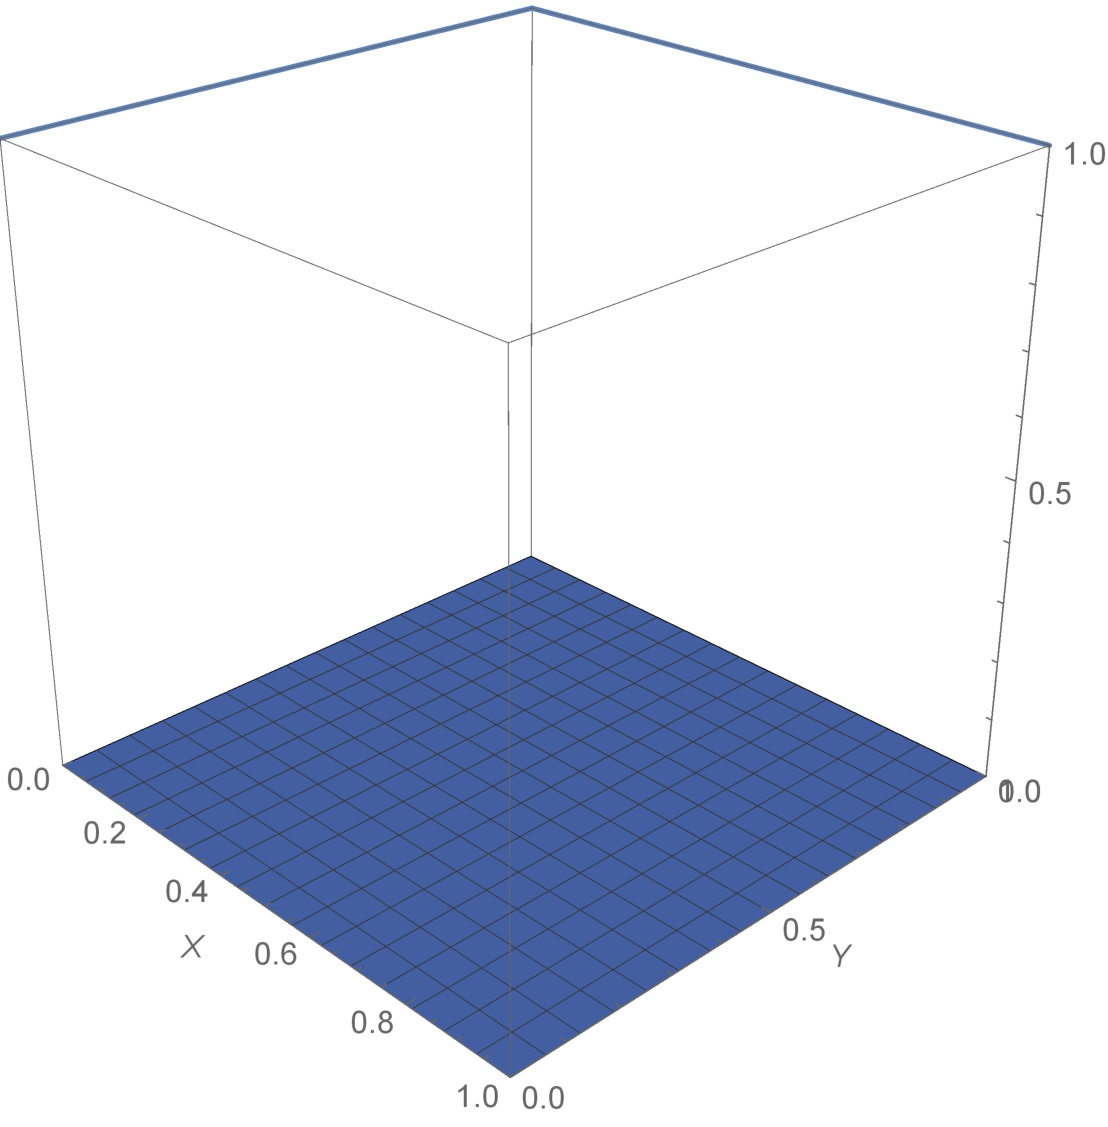
\includegraphics[width=4cm]{ILT.pdf} }
	\subfloat[\IGT]{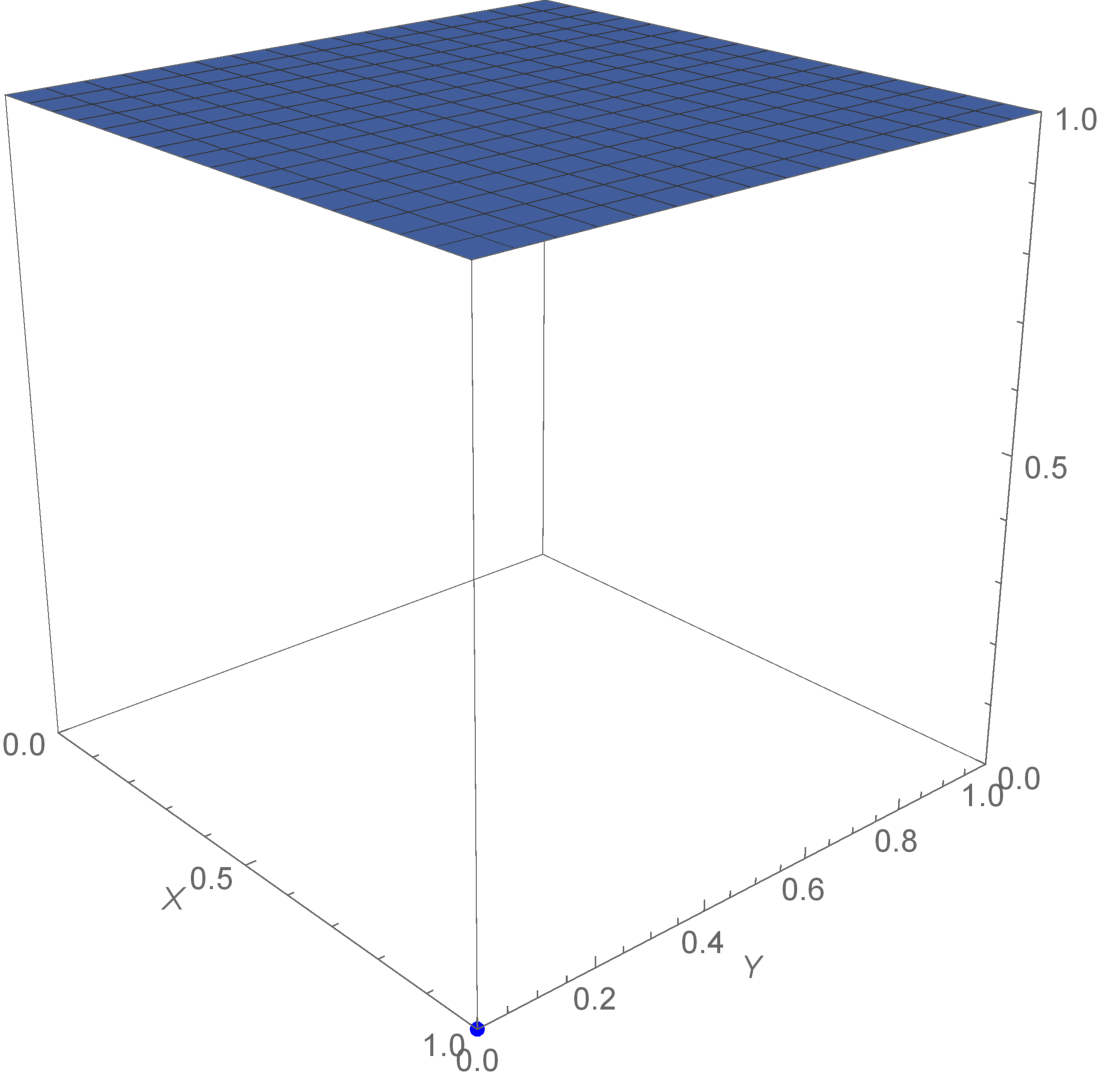
\includegraphics[width=4cm]{IGT.pdf} }
	\caption{Plots of basic fuzzy implication functions presented in Table \ref{table:basic_implications}.}\label{fig:basic_implications}
\end{figure}

\subsection{Families of fuzzy implication functions}\label{subsection:families}

In Table \ref{table:families_FI} we have provided an exhaustive list of families of fuzzy implication functions introduced in the literature and their respective construction methods. Thus, in this section we only take into account those families that are related to the results of this monograph. In particular, we recall the definition and motivation behind the definition of eleven families and we indicate the references in which studies of their additional properties can be found. Since this monograph is partially focused on the study of characterizations, we have recalled here the available characterizations of these families. Some of these characterizations are relatively recent and they are at the forefront of this research line.

\subsubsection{$(S,N)$ and $(U,N)$-implications}

In Section \ref{subsection:definition&additionalproperties} we comment that the generalization of classical tautologies to fuzzy logic is a common method for defining additional properties of fuzzy implication functions. This methodology has also been used as construction method for some families of fuzzy implication functions. For instance, the $S$-implications were introduced in \cite{Trillas1985} as the immediate generalization of the classical Boolean material implication $p \to q \equiv \neg p \vee q$, where the binary disjunction  $\vee $ was modeled by means of a t-conorm and the classical negation $\neg$ was modeled through a strong fuzzy negation $N$. In later studies, this family was generalized to $(S,N)$-implications by considering any fuzzy negation.

\begin{definition}[\textbf{\cite{Trillas1985,Dubois1991,Fodor1994,Klir1995}}]\label{def:(S,N)}
	A function $I:[0,1]^2 \to [0,1]$ is called an \emph{$(S,N)$-implication} if there exist a t-conorm $S$ and a fuzzy negation $N$ such that
	$$I(x,y)=S(N(x),y), \quad x,y \in [0,1].$$
	If $I$ is an $(S,N)$-implication generated from $S$ and $N$, then it is denoted by $I_{S,N}$.
\end{definition}
Since this family of fuzzy implication functions is one of the most important families, a problem of interest throughout the last decades has been to provide a characterization in terms of their properties. Indeed, in \cite{Trillas1985} the authors already provided a characterization for $S$-implications.
\begin{theorem}[\bf{\cite[Theorem 3.2]{Trillas1985}}] 
	Let $I:[0,1]^2\to[0,1]$ be a fuzzy implication function. The following statements are equivalent:
	\begin{enumerate}[label=(\roman*)]
		\item $I$ is an $(S,N)$-implication generated from a continuous t-conorm $S$ and a strong negation $N$.
		\item $I$ satisfies {\bf (NP)}, {\bf (EP)} and {\bf (CP($N$))}.
	\end{enumerate}
\end{theorem}
Later, the authors in \cite{Baczynski2007} provided the characterization of $(S,N)$-implications when $N$ is a continuous negation.
\begin{theorem}[\textbf{\cite[Theorem 5.2]{Baczynski2007}}]\label{th:charac_(S,N)_Ncont}
	For a function $I : [0,1]^2 \to [0,1]$ the following statements are equivalent:
	\begin{enumerate}[label=(\roman*)]
		\item I is an $(S,N)$-implication generated by a t-conorm $S$ and a continuous fuzzy negation $N$.
		\item I satisfies \Ione, \EP and $N_I$ is a continuous fuzzy negation.
	\end{enumerate}	
	Moreover, the representation of the $(S,N)$-implication	 is unique with
	$$N(x)=N_I(x), \quad x \in [0,1],$$
	$$S(x,y)=I(\mathfrak{R}_N(x),y), \quad x,y \in [0,1].$$	
\end{theorem}

However, the characterization of $(S,N)$-implications where $N$ is a non-continuous negation remains an open problem \cite{Baczynski2013,Baczynski2007,Kacprzyk2015}. In Chapter \ref{chapter:chsnimplications} we further discuss this problem.

More generally, in \cite{Pradera2016} the authors study the family of fuzzy implication functions obtained by substituting the role of the classical disjunction in the material implication by any fuzzy disjunction $A$, resulting in the so-called $(A,N)$-implications. Apart from providing a unified view of all the generalizations of $(S,N)$-implications gathered in Table \ref{table:families_FI}, they derive some interesting conclusions. For instance, they prove that there is a one-to-one correspondence between fuzzy implication functions and disjunctors (see \cite[Theorem 40]{Pradera2016}). This result underscores the importance of this construction method. Nonetheless, the most well-known generalization of $(S,N)$-implications is when the t-conorm $S$ is substituted by a disjunctive uninorm, obtaining the family of $(U,N)$-implications.
\begin{definition}[\textbf{\cite[Definition 5.1]{Backzynski2009}}]\label{def:(U,N)}
	A function $I:[0,1]^2 \to [0,1]$ is called a \emph{$(U,N)$-operation} if there exist a uninorm $U$ and a fuzzy negation $N$ such that
	$$I(x,y)=U(N(x),y), \quad x,y \in [0,1].$$
	If $I$ is a $(U,N)$-operation generated from $U$ and $N$, then it is denoted by $I_{U,N}$.
\end{definition}

However, $(U,N)$-operations are fuzzy implication functions only when $U$ is a disjunctive uninorm (see \cite[Theorem 5.3]{Backzynski2009}). Only in this case, we say that $I_{U,N}$ is a $(U,N)$-implication. This family is also characterized only in the case when $N$ is a continuous fuzzy negation (see \cite[Theorem 6.5]{Backzynski2009}).

A study of the additional properties of $(S,N)$ and $(U,N)$-implications can be found in Sections 2.4 and 5.3 of \cite{Baczynski2008}.

% R and RU-implications
%\begin{center}
%	\textsc{$R$ and $RU$-implications}
%\end{center}

\subsubsection{$R$ and $RU$-implications}

Similarly to the introduction of $(S,N)$-implications, $R$-implications were also defined as the generalization of a classical concept. In this case, the focus is on the following identity of crisp set theory:
$$A^c \cup B = (A \setminus B)^c = \bigcup \{C \subseteq X \mid A \cap C \subseteq B\},$$
where $A$ and $B$ are subsets of some universal set $X$. This identity corresponds to an alternative way of defining Boolean implications which is used in intuitionistic logic. The family of $R$-implications generalizes this concept to fuzzy logic.
\begin{definition}[\textbf{\cite{Trillas1985,Dubois1991,Fodor1994,Klir1995}}]\label{def:rimplications}
	A function $I:[0,1]^2 \to [0,1]$ is called an \emph{$R$-implication} if there exists a t-norm $T$ such that
	\begin{equation}\label{eq:rimplications}
	I(x,y)=\sup \{t \in [0,1] \mid T(x,t) \leq y\}, \quad x,y \in [0,1].
	\end{equation}
	If $I$ is an $R$-implication generated from a t-norm $T$, then it is denoted by $I_T$.
\end{definition}
The name of ``$R$-implication'' comes from a very important property related to this family, called the residuation property. However, this property is only satisfied when $T$ is a left-continuous t-norm.
\begin{proposition}[\bf{\cite[Proposition 2.5.2]{Baczynski2008}}]\label{prop:rimpl:residualproperty}
	For a t-norm $T$ the following statements are equivalent:
	\begin{enumerate}[label=(\roman*)]
		\item $T$ is left-continuous.
		\item $T$ and $I_T$ form an adjoint pair, i.e., they satisfy the following residual principle
		$$T(x,z) \leq y \Leftrightarrow I_T(x,y) \geq z, \quad x,y,z\in[0,1]. \eqno {\text{\RP}}$$
		\item The supremum in Equation (\ref{eq:rimplications}) is the maximum, i.e.,
		$$I_T(x,y)=\max \{t \in [0,1] \mid T(x,t) \leq y\}, \quad x,y \in [0,1].$$
	\end{enumerate}
\end{proposition}
The residuation property in Proposition \ref{prop:rimpl:residualproperty} strictly relates the structure of left-continuous t-norms and $R$-implications (see \cite{Jenei1998}). Moreover, in the case of left-continuous t-norms there is also a characterization of $R$-implications.
\begin{theorem}[\bf{\cite{Miyakoshi1985,Fodor1994}}]
	For a function $I:[0,1]^2 \to [0,1]$ the following statements are equivalent:
	\begin{enumerate}[label=(\roman*)]
		\item $I$ is an $R$-implication generated from a left-continuous t-norm.
		\item $I$ satisfies \Itwo, \EP, \OP and it is right-continuous with respect to the second variable.
	\end{enumerate}
\end{theorem}

For the family of $R$-implications there are also several generalizations, which are based on substituting the t-norm by another fuzzy operator. In fact, in \cite{Ouyang2012} the general case in which the role of the t-norm in Definition \ref{def:rimplications} is taken by any binary operator was considered. However, similarly to the case of $(A,N)$-operators, the most well-known generalization of $R$-implications is the one that considers uninorms.

\begin{definition}[\bf{\cite[Definition 5.4.1]{Baczynski2008}}]\label{def:ruoperations}
	A function $I:[0,1]^2 \to [0,1]$ is called an \emph{$RU$-operation} if there exists a uninorm $U$ such that
	$$I(x,y) = \sup \{t \in [0,1] \mid U(x,t) \leq y\}, \quad x,y \in [0,1].$$
	If $I$ is an $RU$-operation generated from a uninorm $U$, then it is denoted by $I_U$.
\end{definition}

Similarly to $(U,N)$-operators, only when $I_U$ is a fuzzy implication function we use the term $RU$-implication. See \cite[Corollary 5.4.4]{Baczynski2008} for some classes of uninorms in which this condition holds. The characterization of $RU$-implications for left-continuous uninorms is also available \cite{Aguilo2010}.

A study of the additional properties of $R$ and $RU$-implications can be found in Sections 2.5 and 5.4 of \cite{Baczynski2008}.

\subsubsection{$QL$ and $D$-implications}
The family of $QL$-implications was introduced as the generalization of the following implication defined in quantum logic: $p \to q \equiv \neg p \vee ( p \wedge q)$.
\begin{definition}[\textbf{\cite[Definition 4]{Mas2006}}]\label{def:QLimplications}
	A function $I:[0,1]^2 \to [0,1]$ is called a \emph{$QL$-operation} if there exist a t-norm $T$, a t-conorm $S$ and a fuzzy negation $N$ such that
	$$I(x,y)=S(N(x),T(x,y)), \quad x,y \in [0,1].$$
	If $I$ is a $QL$-operation generated from the triple $(T,S,N)$, then it is denoted by $I_{T,S,N}$.
\end{definition}
On the other hand, $D$-implications come from the Dishkant arrow: $p \to q \equiv (\neg p \wedge \neg q)\vee q$. 
\begin{definition}[\textbf{\cite[Definition 4]{Mas2006}}]
	A function $I : [0,1]^2 \to [0,1]$ is called a \emph{$D$-operation} if there exist a t-norm $T$, a t-conorm $S$ and a fuzzy negation $N$ such that
	$$I(x,y)=S(T(N(x),N(y)),y), \quad x,y \in [0,1].$$
	If $I$ is a $D$-operation generated from the triple $(S,T,N)$, then is denoted by $I_{S,T,N}$.
\end{definition}

Only when $I_{T,S,N}$ (resp. $I_{S,T,N}$) is a fuzzy implication function we use the term $QL$-implication (resp. $D$-implication). However, unlike other families, there is not an available characterization of those $QL$ or $D$-operators that are fuzzy implication functions, only some partial results are known \cite{Mas2006}. Also, there is no characterization available of these two families, although the characterization of a subclass of $QL$-implications can be found in \cite{Shi2008}.

A study of the additional properties of these two families can be found in \cite[Section 2.6]{Baczynski2008} and \cite{Trillas2000,Trillas2005,Mas2006}.

\subsubsection{Yager's $f$ and $g$-generated, $h$ and $k$-implications}

%% Yager's Implications & h-implications %%
Among those fuzzy implication functions whose definition is based on the use of generator functions, we can highlight Yager's implications, called $f$ and $g$-generated implications. These fuzzy implication functions are generated from additive generators of continuous Archimedean t-norms and t-conorms, respectively.

\begin{definition}[\bf{\cite{Yager2004}}]\label{def:fimpl} 
	Let $f:[0,1] \to [0,+\infty]$ be a strictly decreasing and continuous function with $f(1)=0$. The function $I_f:[0,1]^2 \to [0,1]$ defined by
	$$ I_f(x,y)=f^{-1}(x \cdot f(y)), \quad x,y \in [0,1],$$
	with the understanding $0 \cdot (+ \infty) = 0$, is called an \emph{$f$-generated implication}. The function $f$ itself is called an \emph{$f$-generator}.
	\label{yager_f}
\end{definition}
\begin{definition}[\bf{\cite{Yager2004}}]\label{def:gimpl} 
	Let $g:[0,1] \to [0,+\infty]$ be a strictly increasing and continuous function with $g(0)=0$. The function $I_g:[0,1]^2 \to [0,1]$ defined by
	$$I_g(x,y)=g^{(-1)}\left(\frac{1}{x}\cdot g(y)\right), \quad x,y \in [0,1],$$
	with the understanding $\frac{1}{0}=+\infty$ and $+\infty \cdot 0 = +\infty$ and where the function $g^{(-1)}$ is the pseudo-inverse of $g$ given by
	$$g^{(-1)}(x)=\left \{\begin{array}{ll} g^{-1}(x)& \hbox{if } x \in [0,g(1)],\\ 1&\hbox{if } x \in [g(1),+\infty],\end{array}\right.$$
	 is called a \emph{g-generated implication}. The function $g$ itself is called a \emph{$g$-generator}.
	\label{yager_g}
\end{definition}

In \cite{Yager2004}, Yager gives an extensive analysis of the role of these new classes of implications in approximate reasoning. In particular, he introduces and studies some new interesting concepts like strictness of implications, sharpness of inference, or the strictness index. According to him, these new operators are interesting in approximate reasoning since they accomplish strictness of a fuzzy implication function and sharpness of inference.

The characterization of these two families remained an open problem for almost a decade since the introduction of these classes in \cite{Yager2004} in 2004. They were characterized in 2012 by using the law of importation as the key algebraical property \cite{Massanet2012B}.

\begin{theorem}[\bf{\cite[Theorem 6]{Massanet2012B}}] 
	\label{thm:Char_F_1}
	Let $I:[0,1]^2\to [0,1]$ be a binary function. Then the following statements are equivalent:
	\begin{enumerate}
		\item[(i)] $I$ is an $f$-generated implication with $f(0)<+\infty$.
		\item[(ii)] $I$ satisfies \LI with \TP and $N_I$ is a strict negation.
	\end{enumerate}
	Moreover, in this case the $f$-generator is unique up to a positive multiplicative constant and it is given by $f(x)=N_I^{-1}(x)$. 
\end{theorem}

\begin{theorem}[\bf{\cite[Theorem 12]{Massanet2012B}}] 
	\label{thm:Char_F_Inf}
	Let $I:[0,1]^2\to [0,1]$ be a binary function. Then the following statements are equivalent:
	\begin{enumerate}
		\item[(i)] $I$ is an $f$-generated implication with $f(0)=+\infty$.
		\item[(ii)] $I$ satisfies \LI with \TP, $I$ is continuous except at $(0,0)$ and $I(x,y)=1 \Leftrightarrow x=0 \hbox{ or } y=1$. 
	\end{enumerate}
\end{theorem}

\begin{theorem}[\bf{\cite[Theorem 17]{Massanet2012B}}] 
	\label{thm:Char_G_1}
	Let $I:[0,1]^2\to [0,1]$ be a binary function. Then the following statements are equivalent:
	\begin{enumerate}
		\item[(i)] $I$ is a $g$-generated implication with $g(1)<+\infty$.
		\item[(ii)] $I$ satisfies \LI with \TP and there exists a continuous and strictly increasing function $t:[0,1] \to [0,1]$ with $t(0)=0$ and $t(1)=1$ such that ($I(x,y) = 1 \Leftrightarrow y \geq t(x)$).
	\end{enumerate}
	Moreover, in this case the $g$-generator is unique up to a positive multiplicative constant and it is given by $g(x)=t^{-1}(x)$. 
\end{theorem}

\begin{theorem}[\bf{\cite[Theorem 14]{Massanet2012B}}] 
	\label{thm:Char_G_Inf}
	Let $I:[0,1]^2\to [0,1]$ be a binary function. Then the following statements are equivalent:
	\begin{enumerate}
		\item[(i)] $I$ is a $g$-generated implication with $g(1)=+\infty$.
		\item[(ii)] $I$ satisfies \LI with \TP, $I$ is continuous except at $(0,0)$ and ($I(x,y)=1 \Leftrightarrow x=0 \hbox{ or } y=1$). 
	\end{enumerate}
\end{theorem}

A study of the additional properties of these two families can be found in \cite[Chapter 3]{Baczynski2008}.


Another family of fuzzy implication functions of this kind are the $h$-implications, introduced in \cite{Massanet2011A} following the idea behind the definition of Yager's implications but considering additive generators of representable uninorms.
\begin{definition}[\textbf{\cite[Definition 7]{Massanet2011A}}]\label{Defhimpl} Fix an $e \in (0,1)$ and let $h:[0,1] \to [-\infty,+\infty]$ be a strictly increasing and continuous function with $h(0)=-\infty$, $h(e)=0$ and $h(1)=+\infty$. The function $I^h:[0,1]^2 \to [0,1]$ defined by
	$$I^h(x,y)=\left \{\begin{array}{ll} 1& \hbox{if } x=0,\\
		h^{-1}(x\cdot h(y))&\hbox{if } x>0 \hbox{ and } y \leq e, \\
		h^{-1}(\frac{1}{x}\cdot h(y))&\hbox{if } x>0 \hbox{ and } y > e,
	\end{array}\right.
	$$
	is called an \emph{$h$-implication}. The function $h$ itself is called an \emph{$h$-generator} (with respect to e) of the fuzzy implication function $I^h$ defined as above.
\end{definition}

This family was characterized in \cite{Massanet2012A}. Specifically, it was proved that the characterization of $h$-implications could be derived from the characterization of Yager's implications since the structure of an $h$-implication is given by an $f$ and a $g$-generated implication through the horizontal threshold generation method. The horizontal threshold generation method is a construction method that generates a fuzzy implication function from two given ones and it consists in an appropriate scaling of the second variable of the two fuzzy implication functions.

\begin{theorem}[\textbf{\cite[Theorem 3]{Massanet2012A}}] Let $I_1$, $I_2$ be two fuzzy implication functions and $e \in (0,1)$. Then the binary function $I_{I_1-I_2}:[0,1]^2 \to [0,1]$, called the \emph{$e$-horizontal threshold} generated implication from $I_1$ and $I_2$, defined as
	$$I_{I_1-I_2}(x,y)=\left \{\begin{array}{ll} 1& \hbox{if } x=0,\\
		e \cdot I_1\left(x,\frac{y}{e}\right) &\hbox{if } x>0 \hbox{ and } y \leq e, \\
		e+(1-e)\cdot I_2\left(x,\frac{y-e}{1-e}\right) &\hbox{if } x>0 \hbox{ and } y > e,
	\end{array}\right.
	$$
	is a fuzzy implication function.
	\label{horizontalthreshold}
\end{theorem}

\begin{theorem}[\textbf{\cite[Theorem 2]{Massanet2012A}}]\label{th:characterizationh}
	Let $I:[0,1]^2 \to [0,1]$ be a binary function and $e \in (0,1)$. Then $I$ is an $h$-implication with respect to $e$ if and only if there exist $f$ and $g$-generated implications with $f(0)=g(1)=+\infty$, $I_f$ and $I_g$ respectively, such that $I$ is given by $I=I_{I_f-I_g}$. Moreover, in this case generators $h$, $f$ and $g$ are related in the following way:
	$$f(x)=-h(ex), \quad g(x)=h(e+(1-e)x), \quad \text{for all } x \in [0,1],$$
	$$
	h(x)=\left \{\begin{array}{ll} -f \left(\frac{x}{e}\right)& \hbox{if } x \leq e,\\
		g \left(\frac{x-e}{1-e}\right)&\hbox{if } x>e.
	\end{array}\right.
	$$
\end{theorem}

A study of the additional properties of this family can be found in \cite{Massanet2011A} and \cite[Section 5]{Hlinena2013}.

Another of the families of fuzzy implication functions that we are particularly interested in this monograph is a Yager's related class introduced in 2021 \cite{Zhou2021}. In this paper, the author defines a new family of fuzzy implication functions generated by multiplicative generators of continuous Archimedean t-norms. 

\begin{definition}[\bf{\cite[Definition 8]{Zhou2021}}] 
	Let $k:[0,1]\to[0,1]$ be a strictly increasing and continuous function with $k(1)=1$. The function $I_k : [0,1]^2 \to [0,1]$ defined by
	$$I_k(x,y)=k^{(-1)}\left( \frac{1}{x} \cdot k(y)\right), \quad x,y\in[0,1],$$ 
	with the understanding $\frac{0}{0}=1$ and $\frac{1}{0}=+\infty$ and where $k^{(-1)}$ is the pseudo-inverse of $k$, is called a \emph{$k$-generated implication}. The function $k$ itself is called a \emph{$k$-generator}.
\end{definition}

In the same paper, the author studies several additional properties of this family and he provides the characterization of some subclasses (see \cite[Theorems 2, 5 and 6]{Zhou2021}).

A particularly interesting fact about this family is that, while it is unkown when Yager's implications satisfy \TC, $k$-implications satisfy this property in many cases.

\begin{proposition}[\bf{\cite[Proposition 11]{Zhou2021}}] 
	Let $k$ be a $k$-generator with $k\leq id_{[0,1]}$, $I_k$ the $k$-generated implication and $T_k$ the t-norm generated
	by $k$ as its multiplicative generator. Then, $I_k$ satisfies \TC with
	each t-norm $T$ that is weaker than $T_k$, i.e., $T\leq T_k$.
\end{proposition}

Indeed, in 	\cite[Example 4]{Zhou2021} several pairs of parametric fuzzy implication functions and t-norms that satisfy \TC are provided.

%\begin{center}
%	\textsc{Probabilistic Implications}
%\end{center}

\subsubsection{Probabilistic implications}

In \cite{Grzegorzewski2011,Grzegorzewski2012} new families of fuzzy implication functions with a very interesting and novel origin were introduced. These families  are based on copulas and their definition combines fuzzy concepts and probability theory. According to the author, these families of operators may be useful in situations when we have to cope with imperfect knowledge with both kinds of uncertainty: imprecision and randomness. In particular, four families were defined: probabilistic implications, survival implications, probabilistic $S$-implications and survival $S$-implications. However, in \cite{Massanet2017B} it is proved that the families of probabilistic $S$-implications and survival $S$-implications are equal and in \cite{Massanet2019D} that the families of probabilistic and survival implications are equal. These results were a major breakthrough in the field since from 2011 until 2019 they were studied as different families. This event emphasizes the importance of the study of intersections and characterizations of fuzzy implication functions.

With regard to the results of this monograph, we are interested in probabilistic implications. The idea beyond this family of fuzzy implication functions is first to interpret the probability of an implication as the conditional probability
$$ P(B \mid A) = \frac{P(A \cap B)}{P(A)},$$
and then use the Sklar's theorem to transform the problem into the unit square.

\begin{proposition}[\textbf{\cite[Definition 4 and Theorem 6]{Grzegorzewski2011}}] Let $C$ be a copula. The function $I_C: [0,1]^2 \to [0,1]$ given by
$$I_C(x,y)
=
\left \{\begin{array}{ll} 
	1& \hbox{if } x=0,\\
	\frac{C(x,y)}{x} &\hbox{if } x>0,
\end{array}\right.
$$
is a fuzzy implication function if and only if
$$C(x_1,y)x_2 \geq C(x_2,y)x_1, \quad \text{for all } x_1 \leq x_2 \text{ and } y \in [0,1].$$
In this case, $I_C$ is called a \emph{probabilistic implication} (based on the copula $C$).
\end{proposition}

A study of the additional properties of this family can be found in \cite{Grzegorzewski2011,Grzegorzewski2013,Baczynski2016}. Further, in \cite{Massanet2019D} a characterization of this family was provided.

\begin{theorem}[\textbf{\cite[Theorem 19]{Massanet2019D}}]
	Let $I: [0,1]^2 \to [0,1]$ be a binary function. The following statements are equivalent:
	\begin{enumerate}[label=(\roman*)]
		\item $I$ is a probabilistic implication derived from a copula $C$.
		\item $N_I=\NDOne$ and $I$ satisfies \Ione, \NP, ($I(0,y)=1$ for all $y \in [0,1]$) and
		$$x_2I(x_2,y_1)+x_1I(x_1,y_2) \leq x_1I(x_1,y_1)+x_2I(x_2,y_2),$$
		for all $x_1 \leq x_2$ and $y_1 \leq y_2$.
	\end{enumerate}
\end{theorem}

%% Power-based implications %%

%\begin{center}
%	\textsc{Power-based Implications}
%\end{center}

\subsubsection{Power-based implications}

In Section \ref{subsection:definition&additionalproperties} we define the $T$-power invariance with respect to continuous t-norms \PIT, a property which is relatively novel since it was introduced in 2017 \cite{Massanet2017}. In this same paper, the authors point out that the main families of fuzzy implication functions do not fulfill this property. In this context, they presented $T$-power based implications as a family of fuzzy implication functions defined by a continuous t-norm $T$ and fulfilling the invariance for many choices of $T$ (see \cite{Massanet2017} and its corrigendum \cite{Massanet2019}). 

\begin{definition}[\textbf{\cite[Definition 4]{Massanet2017}}]
	A binary operator $I:[0,1]^2\to[0,1]$ is said to be a \emph{$T$-power based implication} if there exists a continuous t-norm $T$ such that 
	\[
	I(x,y)=\sup \{r \in [0,1] \ | \ y_T^{(r)} \geq x \}\qquad \hbox{for all } \  x, y \in [0,1].
	\]
	If $I$ is a $T$-power based implication, then it is denoted by $I^T$.
\end{definition}
In particular, the structure of $T$-power based implications when is a $T$ continuous Archimedean t-norm is provided by the following proposition.
\begin{proposition}[\bf{\cite[Proposition 5]{Massanet2017}}] Let $T$ be a continuous Archimedean t-norm and $t$ an additive generator of $T$. Then, its power based implication $I^T$ is defined as follows
	$$
	I^T(x,y)
	=
	\left\{ \begin{array}{ll}
		1 &  \text{if }  x \leq y, \\[3pt]
		\frac{t(x)}{t(y)} & \text{if }  x>y,
	\end{array}
	\right.
	$$
	with the convention that $\frac{a}{+\infty}=0$ for all $a \in [0,1]$.
\end{proposition}

A study of the additional properties of this family can be found in \cite{Massanet2017,Massanet2019B,Li2022,Li2023,Peng2022B,Peng2022}. Also, characterizations of this family were presented in \cite{Massanet2019B}, let us recall the corresponding results in the case of continuous Archimedean t-norms.

\begin{proposition}[\bf{\cite[Proposition 17]{Massanet2019B}}]
	Let $I: [0,1]^2 \to [0,1]$ be a binary function. Then $I$ is a $T$-power based implication for some nilpotent t-norm $T$ if and only if the following properties hold:
	\begin{enumerate}[label=(\roman*)]
		\item $I$ satisfies \OP;
		\item $I(x,y) \cdot I(y,0)=I(x,0)$ for all $x>y$;
		\item $I(\cdot,0)$ is a continuous, strictly decreasing function with $I(1,0)=0$.
	\end{enumerate}
	Moreover, in this case the t-norm $T$ is the nilpotent Archimedean t-norm with additive generator $t(x)=I(x,0)$ for all $x \in [0,1]$.
\end{proposition}

\begin{proposition}[\bf{\cite[Proposition 18]{Massanet2019B}}]
	Let $I: [0,1]^2 \to [0,1]$ be a binary function. Then $I$ is a $T$-power based implication for some strict t-norm $T$ if and only if $I$ satisfies \OP and there exists $k \in (0,1]$ such that the following properties hold:
	\begin{enumerate}[label=(\roman*)]
		\item $I(x,y) \cdot I(y,z) = I(x,z)$ for all $x>y>z>0$ and $z<k$;
		\item $\varphi_z : (z,1] \to [0,1]$ defined by $\varphi_z(x)=I(x,z)$ is a continuous, strictly decreasing function for all $0<z<k$;
		\item $I(x,0)=0$ for all $x>0$;
		\item $I(1,y)=0$ for all $y<1$;
		\item $\displaystyle I(x,0)=\lim_{y \to 0^+}I(x,y)$.
	\end{enumerate}
\end{proposition}









 
	%%% Chapter 3
	\chapter{Characterization of generalized $(h,e)$-implications}\label{chapter:heimplications}
	% +--------------------------------------------------------------------+
% | Chapter 03 - Characterization of (h,e)-implications				   |
% +--------------------------------------------------------------------+

\graphicspath{{./_figures/03_heimplications/}}

\section{Introduction}\label{section:introduction(h,e))}

In this chapter, we are interested in the study of the family of generalized $(h,e)$-implications. These fuzzy implication functions were defined for the first time in \cite{Massanet2011A} under the motivation of generalizing $h$-implications to a new family of functions satisfying the property \NPe, that is, $I(e,y)=y$ for all $y \in [0,1]$ and some $e \in (0,1)$.  The family of generalized $(h,e)$-implications has presented very interesting properties such as the controlled increasingness in the second variable by the parameter $e$ or that they constitute a whole family of fuzzy implication functions fulfilling the exchange principle but not the law of importation for any t-norm $T$ \cite{Massanet2011B}. Additionally, they have been applied on image processing for edge detection (see \cite{Gonzalez-Hidalgo2015}), obtaining good results with respect to other families of fuzzy implication functions. Although the properties of $(h,e)$-implications were analyzed for the first time in \cite{Massanet2011A}, in \cite{Hlinena2013} it was pointed out that a more general definition was possible. Therefore, our first contribution is to adapt all the existing results to this more general definition and to provide all the proofs. 

In \cite{Massanet2012A} it was proved that $h$-implications were characterized by the fact that their structure is determined by two Yager's implications through the threshold horizontal method \cite{Massanet2012A}. More specifically, the structure of an $h$-implication is like an adequately scaled $f$-generated implication whenever $y \leq e$ and like an adequately scaled $g$-generated implication whenever $y>e$. In this chapter, as a second contribution, we provide a similar result for $(h,e)$-implications but, in our case,  the structure of $(h,e)$-implications is described in terms of two subfamilies of some new families of fuzzy implication functions which are generalizations of Yager's implications, called $(f,g)$ and $(g,f)$-implications \cite{Massanet2013B}. Until nowadays there has been several proposals of generalizations of Yager's implications by considering different approaches: generalizing the inner factors $x$ and  $\frac{1}{x}$, in the expression of $f$ and $g$-generated implications, respectively \cite{Massanet2013B,VemuriJayaram2012,XieLiu2013,PeiZhu2017}, considering a different internal function from the product \cite{Hlinena2012,Massanet2012C,ZhangLiu2013}; among others \cite{Liu2012,ZhangZhang2017}. The families of $(f,g)$ and $(g,f)$-implications are of the first kind since they consider the internal factor $x$ as a continuous and strictly increasing function $g:[0,1] \to [0,+\infty]$ with $g(0)=0$ and $\frac{1}{x}$ as a continuous and strictly decreasing function $f:[0,1] \to [0,+\infty]$ with $f(0)=+\infty$. This approach is different from all the other generalization proposals, and then the interest in these two families is twofold: to describe the structure of generalized $(h,e)$-implications and to study these families in order to compare their properties with other generalizations considered in the literature. Although these two families were preliminary studied in \cite{Massanet2013B}, the results were provided without any proof and some of them were partially erroneous. Our third contribution is to provide the proofs of all the results and to rectify the mistakes in some statements.

Next, we solve the problem of the characterization of generalized $(h,e)$-implications. To do so, we first provide the characterizations of two subfamilies of $(f,g)$ and $(g,f)$-implications, called $(f,e)$ and $(g,e)$-implications. Consequently, using the representation theorem of generalized $(h,e)$-implications, we provide an axiomatic characterization of this family in terms of their own properties. These three characterizations are based on two novel properties of fuzzy implication functions which are variations of the law of importation different from the generalizations found in the literature \cite{Baczynski2020,Massanet2011B}. In addition, we perform a similar study like the one presented in \cite{Vemuri2014} to provide a representation theorem for $(f,e)$ and $(g,e)$-implications. 

The chapter is structured as follows:  in Section \ref{section:generalized(h,e)impl} the family of generalized $(h,e)$-implications and its main properties are recalled and a proof of the representation theorem is given; in Section \ref{section:(f,g)&(g,f)} the families of $(f,g)$ and $(g,f)$-implications are presented and their properties are studied; in Section \ref{section:characterizations(f,e)&(g,e)} the characterizations of $(f,e)$ and $(g,e)$-implications are presented and in Section \ref{section:representation(f,e)} the representation theorem for $(f,e)$ and $(g,e)$-implications is obtained; in Section \ref{section:characterization(h,e)} the characterization of generalized $(h,e)$-implications is given. The chapter ends in Section \ref{section:conclusionshe} with some conclusions and future work.

\section{Definition and additional properties of generalized $(h,e)$-implications}\label{section:generalized(h,e)impl}

In \cite{Massanet2011A} a new class of fuzzy implication functions was presented, the family of $(h,e)$-implications. The motivation behind its definition was modifying the $h$-implications towards fulfilling the property \NPe. Indeed, the family of $h$-implications presented an unexpected behavior. Most of the families of fuzzy implication functions generated from uninorms such as RU-implications \cite{DeBaets1999}, which are generalizations of R-implications, tend to satisfy \NPe instead of \NP. Being $h$-generators the additive generators of representable uninorms, it would be expected that this family of fuzzy implications functions would satisfy \NPe instead of \NP. This is achieved with a slight modification in the definition leading to the so-called $(h,e)$-implications. 

Although $(h,e)$-implications were first defined in \cite[Definition 7]{Massanet2011A}, in \cite{Hlinena2013} it was pointed out that a more general definition allowing $h(0)>-\infty$ was possible. The latter is the one recalled here.

\begin{definition}[\textbf{\cite[Definition 11]{Hlinena2013}}] Fix an $e \in (0,1)$ and let $h:[0,1] \to [-\infty,+\infty]$ be a strictly increasing and continuous function with $h(e)=0$ and $h(1)= +\infty$. The function $I^{h_g,e}:[0,1]^2 \to [0,1]$ defined by
	$$
	I^{h_g,e}(x,y) = \left\{ \begin{array}{lcl}
		1 &   \hbox{if}  & x=0, \\
		h^{(-1)}\left(\frac{x}{e}h(y)\right)\ &  \hbox{if} & x>0 \text{ and } y\leq e, \\
		h^{-1}\left(\frac{e}{x}h(y)\right) &  \hbox{if}  & x>0 \text{ and } y>e,
	\end{array}
	\right.
	$$
	\noindent where the function $h^{(-1)}$ is the pseudo-inverse of $h$ given by
	$$
	h^{(-1)}(x) = \left\{ \begin{array}{lcl}
		h^{-1}(x) &   \hbox{if}  & x \in [ h(0), + \infty),\\
		0 &  \hbox{if} & x \in (-\infty,h(0)),
	\end{array}
	\right.
	$$
	\noindent is called a \emph{generalized $(h,e)$-implication}. The function $h$ itself is called a \emph{generalized $h$-generator} (with respect to $e$) of the implication function $I^{h_g,e}$ defined as above.
\end{definition}

Although the above definition was proposed in \cite{Hlinena2013} and the properties that were already studied for $(h,e)$-implications in \cite{Massanet2011A} were reconsidered for this more general definition, the results in \cite{Hlinena2013} were announced without any proof. Therefore, hereafter we recall those results but providing the corresponding proof. Having said this, the next proposition ensures that generalized $(h,e)$-implications are indeed fuzzy implication functions.

\begin{proposition}[\textbf{\cite[Proposition 9]{Hlinena2013}}] If $h$ is a generalized $h$-generator with respect to a fixed $e \in (0,1)$, then $I^{h_g,e}$ is a fuzzy implication function.
\end{proposition}
\begin{proof}
	\hspace{0.5cm}
	\begin{itemize}
		\item Let $x_1,x_2,y \in [0,1]$ with $x_1 < x_2$. Since $h$ is strictly increasing we have that $h(x_1) < h(x_2)$ and it holds that $h^{(-1)}$ is an increasing function. Now, we have to distinguish three cases:
		\begin{itemize}
			\item If $x_1=0$ then $ I^{h_g,e}(0,y)=1 \geq I^{h_g,e}(x_2,y)$.
			\item If $x_1 \not = 0$ and $y \leq e$ then $h(y) \leq 0$ and $ \frac{x_1}{e}h(y) \geq  \frac{x_2}{e}h(y)$. Consequently,
			$$ I^{h_g,e}(x_1,y)=h^{(-1)}\left(\frac{x_1}{e}h(y)\right) \geq h^{(-1)}\left(\frac{x_2}{e}h(y)\right) = I^{h_g,e}(x_2,y).$$
			\item If $x_1 \not = 0$ and  $y>e$ then $h(y)>0$ and  $ \frac{e}{x_1}h(y) >  \frac{e}{x_2}h(y)$. Therefore, 
			$$ I^{h_g,e}(x_1,y)=h^{(-1)}\left(\frac{e}{x_1}h(y)\right) \geq h^{(-1)}\left(\frac{e}{x_2}h(y)\right) = I^{h_g,e}(x_2,y).$$
		\end{itemize}
		\item Let $x,y_1,y_2 \in [0,1]$ with $y_1 < y_2$. Then, similarly to the previous point we have that $h(y_1) < h(y_2)$ and we have to consider four different cases:
		\begin{itemize}
			\item If $x=0$ then $I^{h_g,e}(0,y_1)=1=I^{h_g,e}(0,y_2)$.
			\item If $x \not =0$ and $y_1 < y_2 \leq e$ we have that $ h(y_1) < h(y_2) \leq h(e)=0$ and
			$$I^{h_g,e}(x,y_1)=h^{(-1)}\left( \frac{x}{e}h(y_1) \right) \leq  h^{(-1)}\left( \frac{x}{e}h(y_2) \right) = I^{h_g,e}(x,y_1).$$
			\item If $x \not =0$ and $y_1  \leq e < y_2$, we have that $ h(y_1) \leq 0 < h(y_2)$ so $ \frac{x}{e}h(y_1)  \leq 0 <  \frac{e}{x}h(y_2)$ and we get that
			$$I^{h_g,e}(x,y_1)=h^{(-1)}\left( \frac{x}{e}h(y_1)\right) \leq 
			h^{(-1)}(0)=e < h^{-1}\left( \frac{e}{x}h(y_2) \right) = I^{h_g,e}(x,y_2).$$
			\item If $x \not = 0$ and $ e < y_1 <y_2$ then we have that $0 < h(y_1) < h(y_2)$. Thus,
			$$I^{h_g,e}(x,y_1)=h^{-1}\left( \frac{e}{x}h(y_1)\right) \leq 
			h^{-1}\left( \frac{e}{x}h(y_2) \right) = I^{h_g,e}(x,y_2).$$
		\end{itemize}
		\item Finally, $I^{h_g,e}$ satisfies the boundary conditions since
		\begin{itemize}
			\item $I^{h_g,e}(0,0)=1$ by definition.
			\item $I^{h_g,e}(1,1)= h^{-1}\left(\frac{e}{1}h(1)\right) = h^{-1}(+\infty)=1$.
			\item $I^{h_g,e}(1,0)=h^{(-1)}\left(\frac{1}{e}h(0)\right) = 0$.
		\end{itemize}
	\end{itemize}
\end{proof}

Moreover, like in the case of $h$-implications, the generator of a generalized $(h,e)$-implication
is unique up to two positive multiplicative constants.

\begin{proposition}[\textbf{\cite[Proposition 10]{Hlinena2013}}]
	Let $h_1, h_2:[0,1] \to [-\infty,+\infty]$ be two generalized $h$-generators with respect to a fixed $e \in (0,1)$. Then the following statements are equivalent:
	\begin{enumerate}[label=(\roman*)]
		\item $I^{h_{1,g},e}=I^{h_{2,g},e}$.
		\item There exist constants $k,c \in (0,+\infty)$ such that
		$$h_2(x)
		=
		\left\{ \begin{array}{ll}
			k \cdot h_1(x) &   \text{if }   x \in [0,e), \\
			c \cdot h_1(x) &   \text{if }  x \in [e,1].
		\end{array} \right.	
		$$
	\end{enumerate} 
\end{proposition}

\begin{proof}
	The proof is identical to the proof of \cite[Theorem 17]{Massanet2011A}.
\end{proof}
Hereunder, we recall some of the basic properties of generalized $(h,e)$-implications. First of all, the next result studies the natural negation. Notice that in contrast with $(h,e)$-implications, the presence of $h^{(-1)}$ in the more general definition implies that the behavior of the natural negation depends on the value of $h$ in zero.
\pagebreak
\begin{proposition}[\textbf{\cite[Proposition 11]{Hlinena2013}}]\label{prop:naturalnegation(h,e)}
	 Let $h$ be a generalized $h$-generator. Then,
	\begin{enumerate}[label=(\roman*)]
		\item If $h(0)=-\infty$, then the natural negation $N_{I^{h_g,e}}$ is the G\"odel negation or least negation \NDOne.
		\item If $h(0)>- \infty$, then the natural negation $N_{I^{h_g,e}}$ is given by
		$$N_{I^{h_g,e}}(x) = \left\{ \begin{array}{lcl}
			1 &   \hbox{if}  & x=0,\\
			h^{-1}\left(\frac{x}{e}h(0)\right) &  \hbox{if} & x \leq e, \\
			0 &  \hbox{if} & x>e.
		\end{array}
		\right.
		$$
	\end{enumerate}
	\label{negation(h,e)}
\end{proposition}
\begin{proof}
	Let $h$ be a generalized $h$-generator. Then,
	\begin{enumerate}[label=(\roman*)]
		\item If $h(0)=-\infty$, then $h^{(-1)}=h^{-1}$ and for all $x\in [0,1]$ we get
		$$N_{I^{h_g,e}}(x)=I^{h_g,e}(x,0) =  \left\{ \begin{array}{lcl}
			1 &   \hbox{if}  & x=0,\\
			h^{-1}\left(-\infty\right) &  \hbox{if} & x \in (0,1],
		\end{array}
		\right.
		= \left\{ \begin{array}{ll}
			1   &   \text{if } x=0,\\
			0  &   \text{if } x \in (0,1].
		\end{array}
		\right.
		$$
		\item If $h(0)>-\infty$ then we have
		\begin{eqnarray*}
			N_{I^{h_g,e}}(x)
			&=&
			I^{h_g,e}(x,0) =  \left\{ \begin{array}{lcl}
				1 &   \hbox{if}  & x=0,\\
				h^{-1}\left(\frac{x}{e}h(0)\right) &  \hbox{if} & \frac{x}{e}h(0) \geq h(0), \\
				0 &  \hbox{if} & \frac{x}{e}h(0) < h(0),
			\end{array}
			\right. \\
			&=& \left\{ \begin{array}{ll}
				1 &   \text{if } x=0,\\
				h^{-1}\left(\frac{x}{e}h(0)\right)&   \text{if } x \leq e, \\
				0 &   \text{if } x>e.
			\end{array}
			\right.
		\end{eqnarray*}
	\end{enumerate}	
\end{proof}

The following proposition studies when generalized $(h,e)$-implications fulfill some additional properties of fuzzy implication functions.

\begin{theorem}[\textbf{\cite[Theorem 22]{Hlinena2013}}]\label{th:AddProp(h,e)} Let $h$ be a generalized $h$-generator and $e \in (0,1)$. The following properties hold:
	\begin{enumerate}[label=(\roman*)]
		\item $I^{h_g,e}(x,y) \leq e$ if and only if $(x>0 \hbox{ and } y \leq e)$. Moreover $I^{h_g,e}(x,e)=e$ for all $x>0$.
		\item $I^{h_g,e}$ satisfies {\bf (EP)} if and only if $h(0)=-\infty$.
		\item $I^{h_g,e}(x,y)=1$ if and only if $x=0$ or $y=1$. Thus, $I^{h_g,e}$ does not satisfy either {\bf (OP)} or {\bf (IP)}.
		\item $I^{h_g,e}$ is continuous except at the points $(0,y)$ with $y \leq e$.
		\item $I^{h_g,e}$ satisfies \NPe but does not satisfy {\bf (NP)}.
		\item $I^{h_g,e}$ does not satisfy \LI with respect to any t-norm $T$.
		\item $I^{h_g,e}$ does not satisfy {\bf (CP(N))} with any fuzzy negation $N$.
	\end{enumerate}
	\label{propietats1(h,e)}
\end{theorem}
\begin{proof}
	\hspace{0.5cm}
	\begin{enumerate}[label=(\roman*)]
		\item It is clear that if $x>0$ and $y \leq e$ then $I^{h_g,e}(x,y)= h^{(-1)}\left(\frac{x}{e}h(y) \right) \leq e$ since $h(y) \leq 0$. Otherwise, if $x=0$, $I^{h_g,e}(0,y)=1$ for all $y \in [0,1]$ and if $x>0$ and $y>e$, $I^{h_g,e}(x,y)=h^{-1}\left(\frac{e}{x}h(y) \right)>e$ because $h(y)>0$. Moreover we have that $I^{h_g,e}(x,e)=h^{(-1)}\left(\frac{x}{e}h(e)\right)=h^{(-1)}(0)=e$ for all $x>0$.
		\item Assume that $I^{h_g,e}$ satisfies {\bf (EP)}. Now, let us consider $h(0)>-\infty$ and we will get a contradiction. Let us fix an $x_0 \in (0,e^2)$, notice that 
		$$ x_0 <e^2 \Rightarrow x_0 <e \Rightarrow \frac{x_0}{e}h(0) > h(0) \Rightarrow I^{h_g,e}(x_0,0)= h^{-1}\left(\frac{x_0}{e}h(0)\right).$$
		
		On the one hand, we have
		$$I^{h_g,e}(x_0,I^{h_g,e}(1,0))= I^{h_g,e}(x_0,0) = h^{-1}\left(\frac{x_0}{e}h(0)\right).$$
		
		On the other hand, since $x_0<e^2$ and by Point (i) $I^{h_g,e}(x_0,0) \leq e$ we get 
		$$I^{h_g,e}(1,I^{h_g,e}(x_0,0)) = I^{h_g,e}\left(1,h^{-1}\left(\frac{x_0}{e}h(0)\right)\right)
		=h^{(-1)}\left(\frac{x_0}{e^2}h(0)\right) = h^{-1}\left(\frac{x_0}{e^2}h(0)\right).
		$$
		Thus, since we have that $h^{-1}$ is strictly increasing in $[h(0),+\infty]$ we get that 
		$$ h^{-1}\left(\frac{x_0}{e^2}h(0) \right) < h^{-1}\left(\frac{x_0}{e}h(0) \right).$$
		Hence, $I^{h_g,e}(1,I^{h_g,e}(x_0,0)) < I^{h_g,e}(x_0,I^{h_g,e}(1,0))$. Contradiction with the fact that $I^{h_g,e}$ satisfies \EP.\\
		For the reverse implication, if $h(0)=-\infty$ we know that in this case $h^{(-1)}=h^{-1}$ and $N_{I^{h_g,e}}=\NDOne$. For any $x,y,z \in [0,1]$, let us distinguish five cases:
		\begin{itemize}
			\item If $x=0$ then for all $y,z \in [0,1]$ we have that
			$$I^{h_g,e}(0,I^{h_g,e}(y,z))=1=I^{h_g,e}(y,1)= I^{h_g,e}(y,I^{h_g,e}(0,z)).$$
			\item If $y=0$ for all $x,z \in [0,1]$ we have that
			$$I^{h_g,e}(x,I^{h_g,e}(0,z))=I^{h_g,e}(x,1)= 1=I^{h_g,e}(0,I^{h_g,e}(x,z)).$$
			\item If $ x \not = 0$, $y \not = 0$ and $z=0$, we obtain
			\begin{eqnarray*}
				I^{h_g,e}(x,I^{h_g,e}(y,0))&=&I^{h_g,e}(x,N_{I^{h_g,e}}(y))= I^{h_g,e}(x,0)=N_{I^{h_g,e}}(x)=0 \\
				&=&N_{I^{h_g,e}}(y)=I^{h_g,e}(y,0)=I^{h_g,e}(y,N_{I^{h_g,e}}(x))\\
				&=&I^{h_g,e}(y,I^{h_g,e}(x,0)).
			\end{eqnarray*}
			\item If $x \not = 0$, $y \not = 0$ and $0<z \leq e$, by Point (i), $I^{h_g,e}(y,z) \leq e$ and $I^{h_g,e}(x,z) \leq e$  and consequently
			$$I^{h_g,e}(x,I^{h_g,e}(y,z))=I^{h_g,e}\left(x,h^{-1}\left(\frac{y}{e}h(z)\right)\right) = h^{-1}\left(\frac{xy}{e^2}h(z)\right).$$
			Similarly,
			$$I^{h_g,e}(y,I^{h_g,e}(x,z))=I^{h_g,e}\left(y,h^{-1}\left(\frac{x}{e}h(z)\right)\right) = h^{-1}\left(\frac{xy}{e^2}h(z)\right).$$
			\item Finally, if $x \not = 0$, $y \not = 0$ and $e<z\leq 1$, then again by (i) we have $I^{h_g,e}(y,z)>e$ and $I^{h_g,e}(x,z)>e$ and thus
			$$I^{h_g,e}(x,I^{h_g,e}(y,z))=I^{h_g,e}\left(x,h^{-1}\left(\frac{e}{y}h(z)\right)\right) = h^{-1}\left(\frac{e^2}{xy}h(z)\right),$$
			$$I^{h_g,e}(y,I^{h_g,e}(x,z))=I^{h_g,e}\left(y,h^{-1}\left(\frac{e}{x}h(z)\right)\right) = h^{-1}\left(\frac{e^2}{xy}h(z)\right).$$
		\end{itemize}
		\item It is obvious that if $x=0$ or $y=1$, $I^{h_g,e}(x,y)=1$ since $I^{h_g,e}$ is a fuzzy implication function. If $x \not = 0$ and $y \leq e$, by Point (i) we have $I^{h_g,e}(x,y) \leq e <1$. If $x \not = 0$ and $e <y <1$ then $0< h(y) < + \infty$ and we get that
		$$I^{h_g,e}(x,y)= h^{-1}\left(\frac{e}{x}h(y)\right) < h^{-1}(+\infty)=1.$$
		\item By definition, the implication $I^{h_g,e}$ is continuous for all $(x,y) \in (0,1] \times [0,e)$ and for all $(x,y) \in (0,1] \times (e,1]$. 
		Further, the vertical sections with  a fixed $x>0$ are continuous since
		$$I^{h_g,e}(x,e) = h^{(-1)}\left(\frac{x}{e}h(e)\right) = h^{(-1)}(0)=e,$$
		and
		$$\lim_{y \to e^{-}} I^{h_g,e}(x,y) = \lim_{y \to e^-} h^{(-1)}\left(\frac{x}{e}h(y)\right) = h^{(-1)}(0)=e,$$
		$$\lim_{y \to e^{+}}I^{h_g,e}(x,y) = \lim_{y \to e^+} h^{-1}\left(\frac{e}{x}h(y)\right) = h^{-1}(0)=e.$$
		On the other hand, the horizontal sections with $y>e$ are continuous since $I^{h_g,e}(0,y)=1$ and
		$$\lim_{x \to 0^{+}}I^{h_g,e}(x,y) = \lim_{x \to 0^+} h^{-1}\left(\frac{e}{x}h(y)\right) = h^{-1}(+\infty)=1.$$
		However, for a fixed $y \in(0,1)$ such that $0 < y \leq e$ and $- \infty < h(y) \leq 0$ we know that $I^{h_g,e}(0,y)=1$, but
		$$\lim_{x \to 0^{+}} I^{h_g,e}(x,y) = \lim_{x \to 0^+} h^{(-1)}\left(
		\frac{x}{e}h(y)\right) = h^{(-1)}(0)=e.$$
		Thus, horizontal sections of $I^{h_g,e}$ with $y \leq e$ are continuous expect at the points $(0,y)$ with $0 <y \leq e$. Finally, by Proposition \ref{negation(h,e)}, $I^{h_g,e}$ is not continuous also at the point $(0,0)$. Now, applying Theorem \ref{theorem:A04} adequately, we can prove that $I^{h_g,e}$ is continuous except at the points $(0,y)$ with $y \leq e$.
		\item For all $y \in [0,1]$ we have that
		$$I^{h_g,e}(e,y)= \left\{ \begin{array}{lcl}
			h^{(-1)}\left(h(y)\right) &   \hbox{if}  & y \leq e,\\
			h^{-1}\left(h(y)\right) &  \hbox{if} & y > e,
		\end{array}
		\right. = y.
		$$
		Thus, $I^{h_g,e}$ satisfies \NPe. On the other hand, for all $y >e$ we have that
		$$I^{h_g,e}(1,y) =y \Leftrightarrow h^{-1}(eh(y))=y \Leftrightarrow eh(y)=h(y) \Leftrightarrow e=1.$$
		Thus $I^{h_g,e}$ does not satisfy \NP.
		\item  Suppose that $I^{h_g,e}$ fulfills \LI with respect to a t-norm $T$, then we know that it also fulfills  \EP and by Point (ii), $h(0)=-\infty$. Now, taking $x=y=1$ and $e<z<1$, since $T(1,1)=1$ we have that
		$$I^{h_g,e}(T(1,1),z)= I^{h_g,e}(1,I^{h_g,e}(1,z)) \Leftrightarrow h^{-1} (eh(z))=h^{-1} (e^2h(z)) \Leftrightarrow e=1.$$
		Thus, $I^{h_g,e}$ does not satisfy \LI with respect to any t-norm $T$.
		\item Suppose that $I^{h_g,e}$ satisfies {\bf (CP(N))} with a fuzzy negation $N$. So, we have $I^{h_g,e}(x,y)=I^{h_g,e}(N(y),N(x))$ for all $x,y \in [0,1]$. Taking $x=1$ and $y=e$, we know by Point (i) that $I^{h_g,e}(1,e)=e$ and then 
		$$e=I^{h_g,e}(1,e)=I^{h_g,e}(N(e),N(1))=I^{h_g,e}(N(e),0)=N_{I^{h_g,e}}\circ N(e).$$ 
		If $h(0)=-\infty$ then $N_{I^{h_g,e}}=\NDOne$ and we obtain a contradiction. If $h(0) > - \infty$ then 
		$$e= N_{I^{h_g,e}}\circ N(e) =
		\left\{ \begin{array}{ll}
			1 & \text{if } N(e)=0, \\
			h^{-1}\left(\frac{N(e)}{e}h(0)\right) &   \text{if } N(e)\leq e, \\
			0 &   \text{if } N(e)>e, 
		\end{array}
		\right.
		$$
		and the only feasible case is $N(e) \in (0,e]$ and then $N(e)h(0)=h(e) \cdot e=0$ which is also a contradiction.
	\end{enumerate}
\end{proof}

Perhaps one of the main properties of $(h,e)$-implications is given by (i) in the previous theorem. It reflects that these operators have a controlled increasingness with respect to the second variable produced by the insertion of the parameter $e$, as we can graphically see in Figure \ref{exempl(h,e)}. Observe that the fuzzy implication functions generated by the horizontal threshold method in Theorem \ref{horizontalthreshold} had a similar property, so it is intuitive to think that generalized $(h,e)$-implications are related in some way with this method. Also, notice that the family of generalized $(h,e)$-implications provides an example of fuzzy implication functions which do not satisfy \LI with respect to any t-norm $T$ and yet satisfy \EP when $h(0)=-\infty$, providing another argument of the fact that \LI is stronger than \EP \cite{Massanet2011B}.

\begin{example} Let us consider the generalized $h$-generator
	$$h(x)=
	\left\{ \begin{array}{ll}
		\ln \left(\frac{x}{e}\right) &   \text{if } x\leq e, \\
		-\ln \left( \frac{1-x}{1-e}\right) &   \text{if } x>e, 
	\end{array}
	\right.
	$$
	with $e \in (0,1)$. The corresponding generalized $(h,e)$-implication is the following one
	\begin{equation}
		I^{h_g,e}(x,y) = \left\{ \begin{array}{ll}
			1 &   \text{if } x=0, \\
			e\left(\frac{y}{e}\right)^{\frac{x}{e}} &   \text{if } x>0,y\leq e, \\
			1-(1-e)\cdot \left(\frac{1-y}{1-e}\right)^{\frac{e}{x}} &   \text{if } x>0,y>e. 
		\end{array}
		\right.
		\label{exemple(h,e)}
	\end{equation}
	The plot of this generalized $(h,e)$-implication for different values of the parameter $e$ can be seen in Figure \ref{exempl(h,e)}.
	\begin{figure}[H]
		\centering
		\subfloat[\centering $e=0.25$]{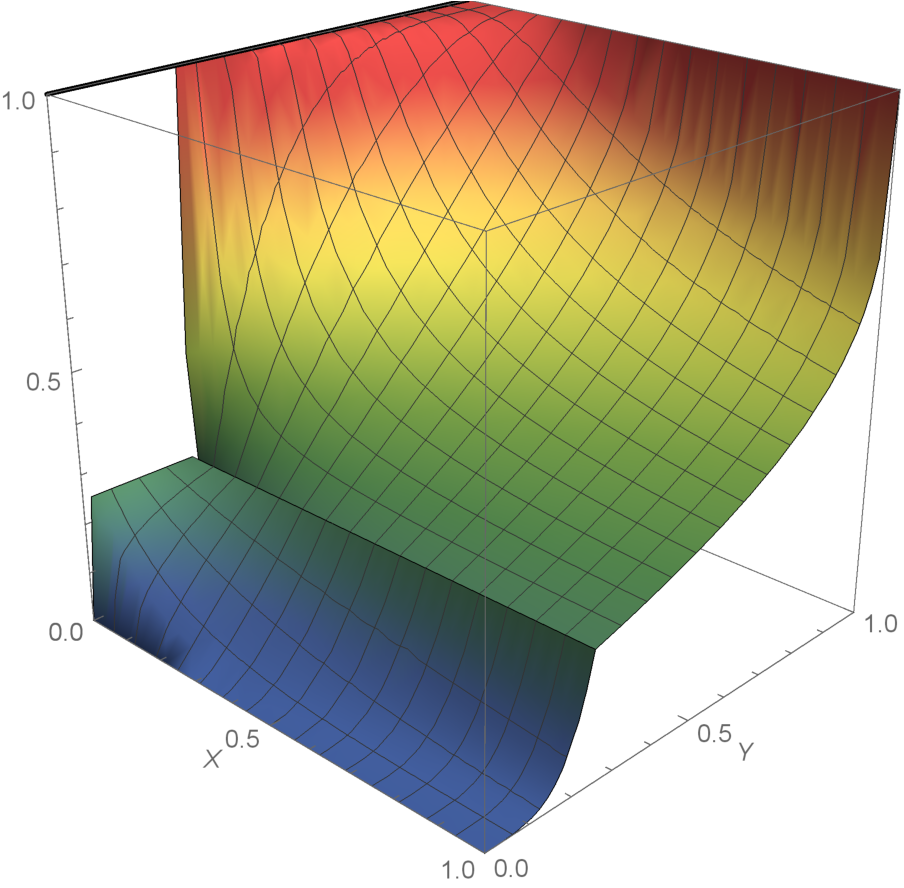
\includegraphics[width=4cm]{he1.pdf} }
		\subfloat[\centering $e=0.5$]{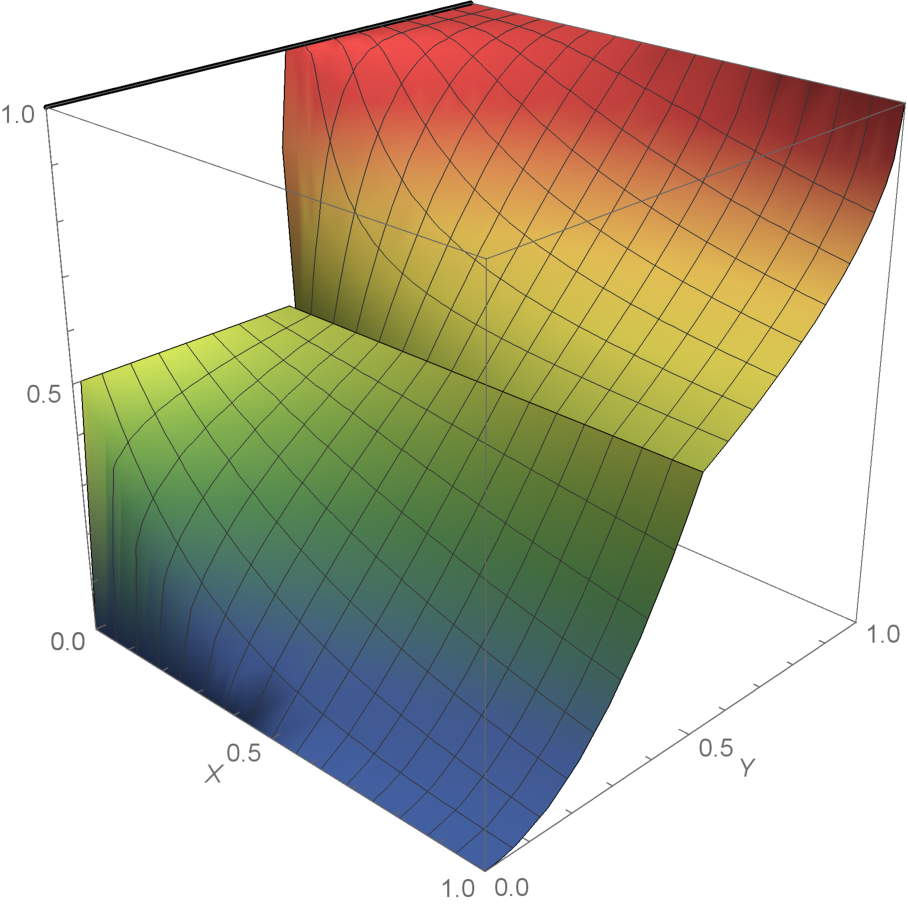
\includegraphics[width=4cm]{he2.pdf} }
		\subfloat[\centering $e=0.75$]{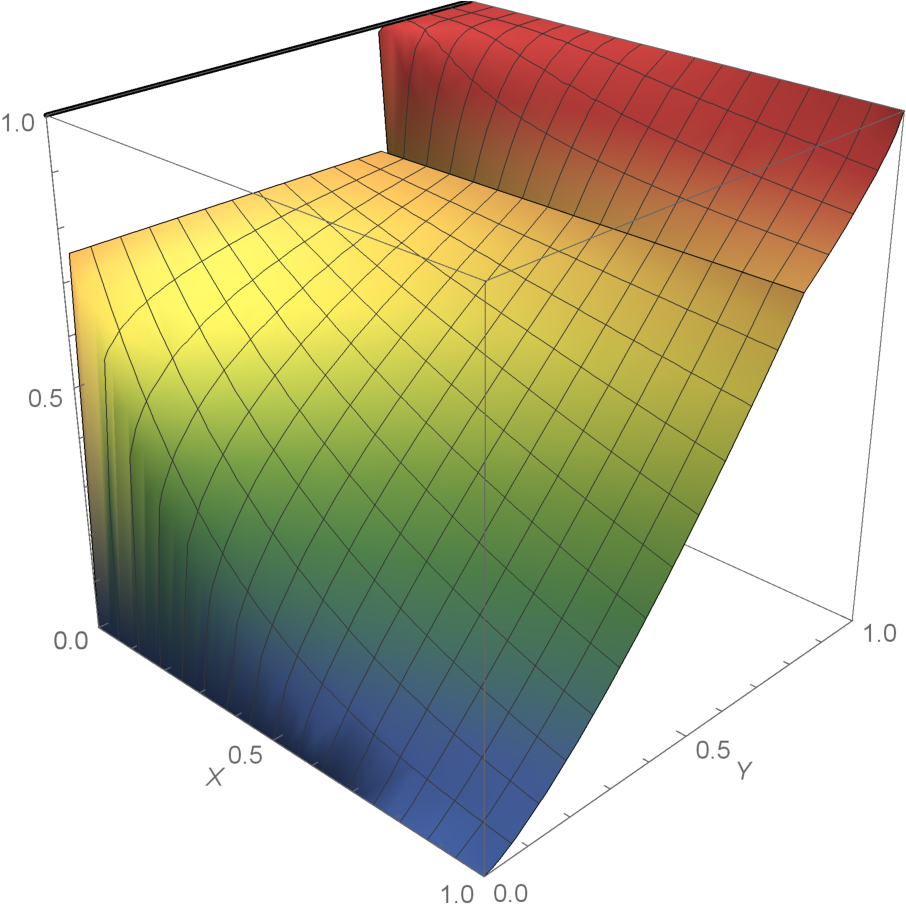
\includegraphics[width=4cm]{he3.pdf} }\\
		\caption[Plot of a generalized $(h,e)$-implication for different values of $e$.]{Plot of the generalized $(h,e)$-implication given by Equation (\ref{exemple(h,e)}) for different values of $e$.}\label{exempl(h,e)}
	\end{figure}
	\label{controlledincreasingness}
\end{example}

\subsection{Representation theorem}\label{subsection:representation_theorem}

Although prior to this study no axiomatic characterization of $(h,e)$-implications was available in the literature, in \cite{Massanet2013B} a representation theorem for this family was presented without the corresponding proof. In this section, we provide a proof for that result and we adjust it to the case of generalized $(h,e)$-implications.

\begin{theorem}\label{ThmRepresentacio(h,e)}
	Let $I:[0,1]^2 \to [0,1]$ be a binary function and $e \in (0,1)$. Then $I$ is a generalized $(h,e)$-implication with respect to $e$ if and only if there exist an $f$-generator and a $g$-generator with $g(1)=+\infty$ such that $I$ is given by
	\label{ThmRep(h,e)}
	\begin{equation}
		I(x,y) = \left\{ \begin{array}{lcl}
			1 &   \hbox{if}  & x=0, \\
			e \cdot f^{(-1)}\left(\frac{x}{e} \cdot f\left( \frac{y}{e}\right)\right)\ &  \hbox{if} & x>0,y\leq e, \\
			e+(1-e)\cdot g^{-1}\left( \frac{e}{x} \cdot g \left(\frac{y-e}{1-e}\right)\right) &  \hbox{if}  & x>0,y>e.
		\end{array}
		\right.
		\label{eq4}
	\end{equation}
	Moreover, in this case generators $h$, $f$ and $g$ are related in the following way
	
	$$f(x)=-h(e\cdot x), \quad \text{for all } x \in [0,1], \quad g(x)=h(e+(1-e)\cdot x), \quad \text{for all } x \in [0,1],$$
	
	$$ h(x) =  \left\{ \begin{array}{lcl}
		-f\left(\frac{x}{e} \right) &   \hbox{if}  & x \leq e, \\
		g\left(\frac{x-e}{1-e}\right) &  \hbox{if} & x>e.
	\end{array}
	\right.
	$$
\end{theorem}

\begin{proof}
	Let $I$ be a generalized $(h,e)$-implication with respect to $e$. We know that $h$ is a continuous and strictly increasing function with $h(e)=0$ and $h(1)=+\infty$. First of all, note that $f(x)=-h(ex)$ and $g(x)=h(e+(1-e)x)$ are $f$ and $g$-generators, respectively, since $f$ is a continuous and strictly decreasing function with $f(1)=-h(e)=0$ and $g$ is a continuous and strictly increasing function with $g(0)=h(e)=0$.  Note that since $h^{-1}$ is well defined on $[h(0), +\infty)$ with $h(0)<0$ then we have for all $ x \in [0, +\infty)$ that
	$$ f^{(-1)}(x) = \frac{h^{(-1)}(-x)}{e}, \quad g^{-1}(x) = \frac{h^{-1}(x)-e}{1-e}.$$
	For $x=0$ it is clear that $I(0,y)=1$ for all $y \in [0,1]$ and $I$ corresponds to Equation (\ref{eq4}) on these points. For the situation $x>0$ we will split the proof in two cases:
	\begin{itemize}
		\item If $x>0$ and $y \leq e$ then
		$$ e f^{(-1)} \left(\frac{x}{e}f\left(\frac{y}{e}\right) \right) = ef^{(-1)}\left(-\frac{x}{e}h(y)\right)= h^{(-1)} \left(\frac{x}{e}h(y) \right) = I(x,y).$$
		\item If $x>0$ and $ y > e$ then
		\begin{eqnarray*}
			e + (1-e) \cdot g^{-1}\left(\frac{e}{x}g\left(\frac{y-e}{1-e}\right)\right) &=& e + (1-e) \cdot \frac{h^{-1}\left( \frac{e}{x} h\left(e+(1-e) \frac{y-e}{1-e} \right)\right)-e}{1-e} \\
			&=& h^{-1} \left(\frac{e}{x}h(y) \right) = I(x,y).
		\end{eqnarray*}
	\end{itemize}
	For the reverse implication, let us consider $f$ and $g$-generators such that $I$ is given by Equation (\ref{eq4}). Consider
	$$h(x) = \left\{ \begin{array}{lcc}
		-f\left(\frac{x}{e} \right) &   \hbox{if}  & x \leq e, \\
		g \left( \frac{x-e}{1-e} \right) &  \hbox{if} & x>e .
	\end{array}
	\right.
	$$
	This function is continuous, strictly increasing, $h(e)=-f(1)=0$ and $h(1)=g(1)= + \infty$. Now, let us prove that $I = I^{h_g,e}$. Notice that
	\begin{eqnarray*}
		h^{(-1)}(x) &=& \left\{ \begin{array}{lcc}
			h^{-1}(x) &   \hbox{if}  & x \in [h(0), + \infty), \\
			0 &  \hbox{if} & x \in (- \infty, h(0)) ,
		\end{array}
		\right. \\
		&=&
		\left\{ \begin{array}{lcc}
			0 &  \hbox{if} & x \in (- \infty, -f(0)) , \\
			e \cdot f^{-1}(-x) &   \hbox{if}  & x \in [-f(0), 0], \\
			e+(1-e) \cdot g^{-1}(x) &  \hbox{if} & x \in (0, + \infty).
		\end{array}
		\right.
	\end{eqnarray*}
	Then, studying again two cases we have that
	\begin{itemize}
		\item If $x>0$ and $y \leq e$ then
		$$I^{h_g,e}(x,y)= h^{(-1)} \left(\frac{x}{e} h(y) \right) = h^{(-1)} \left(- \frac{x}{e} f \left( \frac{y}{e} \right) \right) = e \cdot f^{(-1)} \left(\frac{x}{e} f \left(\frac{y}{e} \right) \right)  = I(x,y).$$
		\item If $x>0$ and $y>e$ then
		\begin{eqnarray*}
			I^{h_g,e}(x,y) &=& h^{-1} \left(\frac{e}{x}h(y) \right) = h^{-1} \left(\frac{e}{x} g \left( \frac{y-e}{1-e}\right) \right) = e + (1-e) \cdot g^{-1} \left( \frac{e}{x} g \left( \frac{y-e}{1-e}\right) \right) \\
			&=&I(x,y).
		\end{eqnarray*}
	\end{itemize}
\end{proof}

The next example provides the construction of a generalized $(h,e)$-implication by using the threshold horizontal method given an $f$-generator and a $g$-generator with $g(1)=+\infty$.
\begin{example} Let us consider $e=\frac{1}{2}$ and the subsequent $f$ and $g$-generators
	
	$$ f(x)= - \ln \left( \frac{x}{2-x} \right), \quad g(x)=\ln \left( \frac{1+x}{1-x}\right).$$
	It is easy to check that the following functions are fuzzy implication functions
	$$I_1(x,y)=f^{(-1)}\left(\frac{x}{e} f(y)\right)= \frac{2y^{2x}}{(2-y)^{2x}+y^{2x}},$$
	$$ I_2(x,y)=\quad g^{-1}\left(\frac{e}{x}g(y)\right)=\frac{(1+y)^{\frac{1}{2x}}-(1-y)^{\frac{1}{2x}}}{(1+y)^{\frac{1}{2x}}+(1-y)^{\frac{1}{2x}}}.$$
	Then, a generalized $(h,e)$-implication is constructed from $I_1$ and $I_2$ by using the threshold horizontal method as described in Theorem \ref{ThmRepresentacio(h,e)}. Concretely, the $h$-generator corresponds to  
	$$h(x)=  \ln \left( \frac{x}{1-x}\right).$$
	We can see the construction method graphically in Figure \ref{thresholdimpl}.
	
	\begin{figure}[H]
		\centering
		\subfloat[\centering $I_1$]{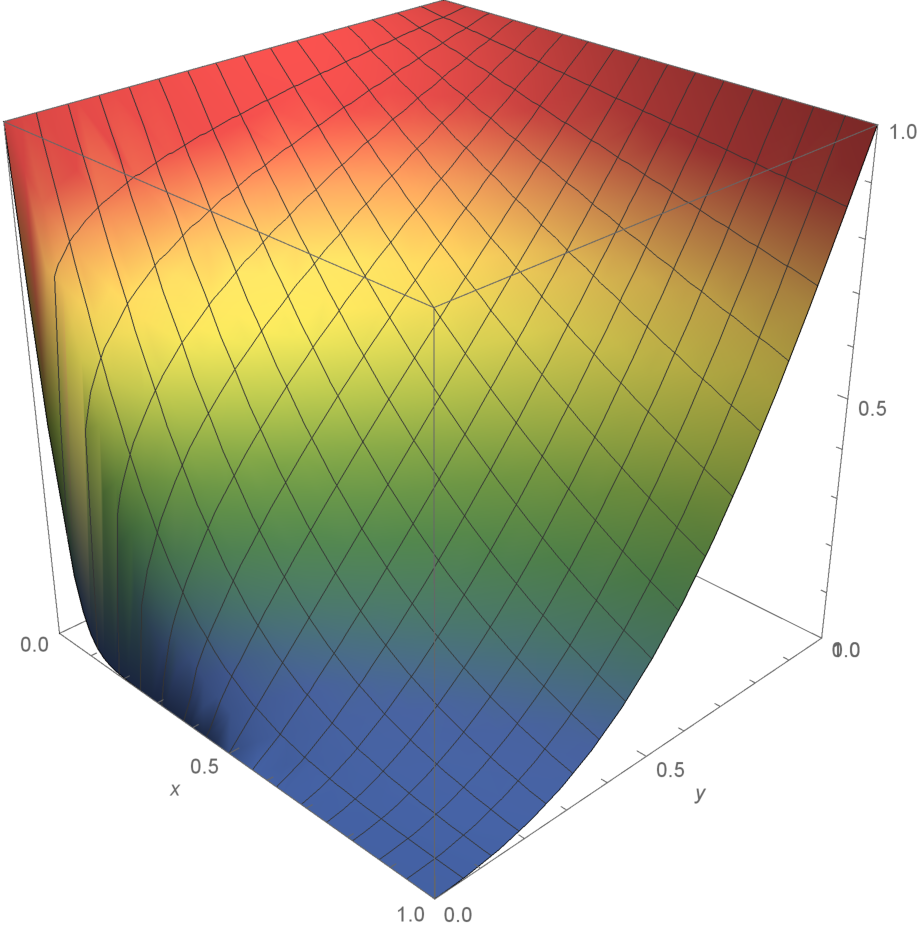
\includegraphics[width=4cm]{fe1.pdf} }
		\subfloat[\centering $I_2$]{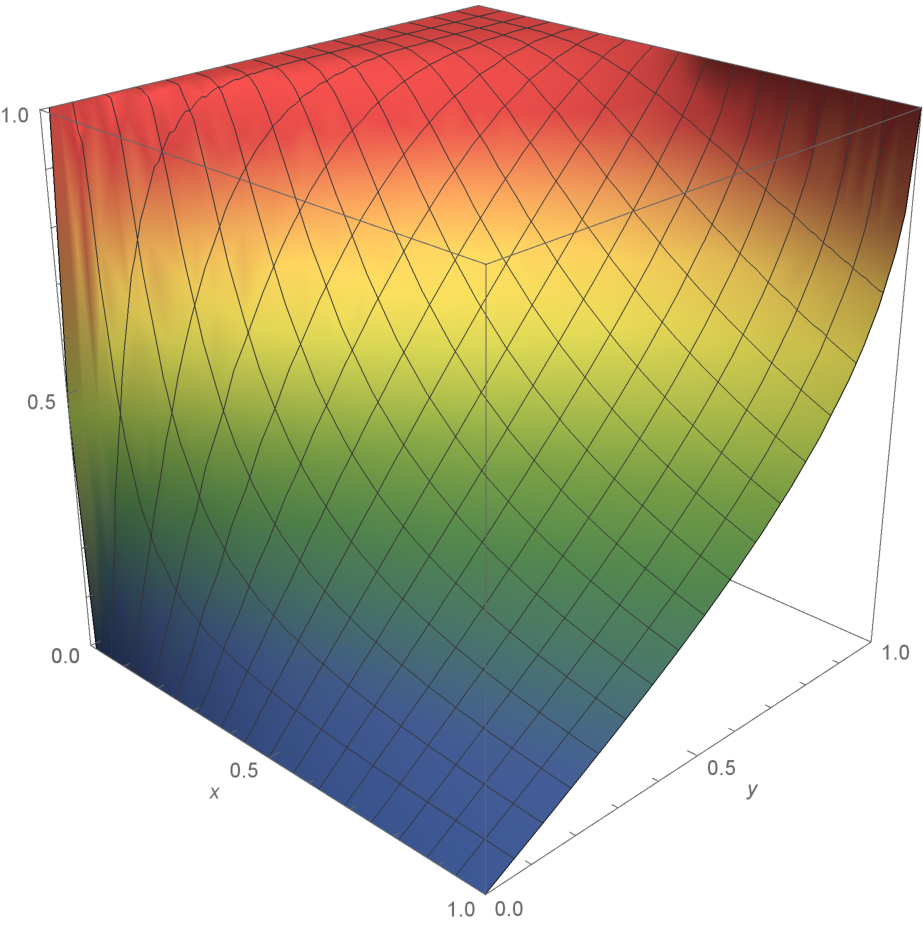
\includegraphics[width=4cm]{ge1.pdf} }
		\subfloat[\centering $I^{h,e} = I_{I_1-I_2}$]{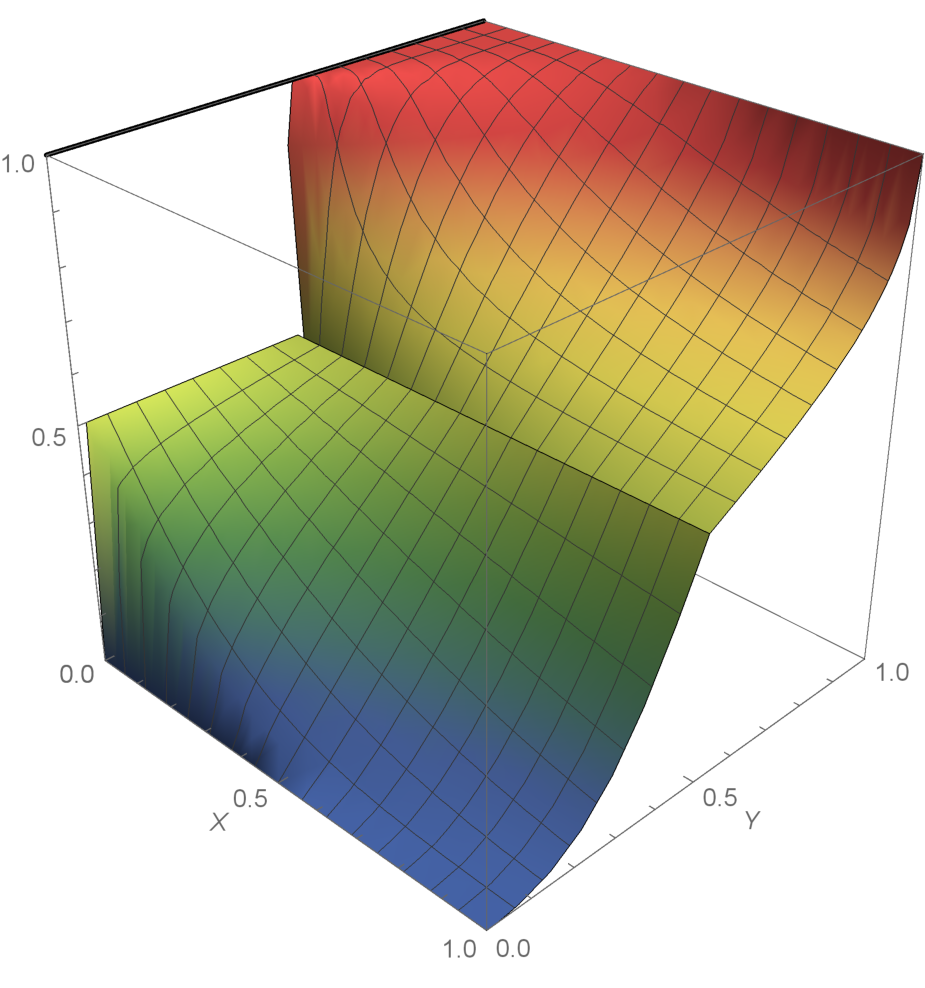
\includegraphics[width=4cm]{he.pdf} }\\
		
		\caption[Plot of a generalized $(h,e)$-implication constructed via the horizontal threshold method jointly with the two fuzzy implication functions that act as generators.]{Plot of a generalized $(h,e)$-implication with $e=\frac{1}{2}$ constructed via the horizontal threshold method jointly with the two fuzzy implication functions $I_1$, $I_2$ that act as generators.}\label{thresholdimpl}
	\end{figure}
	\label{ExempleRepresentació(h,e)}
\end{example}

Although Theorem \ref{ThmRepresentacio(h,e)} gives a useful description of the family of generalized $(h,e)$-implications, it is not an axiomatic characterization of this family, i.e., a characterization in terms of their own properties. For providing such result, a deeper study of this family is needed.

Let us recall that the characterization of $h$-implications presented in \cite{Massanet2012A} was written in terms of the threshold horizontal method, in particular $h$-implications are characterized by the fact that they are generated by an $f$-implication and a $g$-implication through the horizontal threshold method. In this case, the axiomatic characterization was not provided but it can be easily obtained by using the characterizations of Yager's implications presented in \cite{Massanet2012B}. For the case of generalized $(h,e)$-implications, it is straightforward to prove that if we consider an $f$-generator, the function $I_{f,e}:[0,1]^2 \to [0,1]$ defined by
$$I_{f,e}(x,y)=f^{(-1)}\left(\frac{x}{e}f(y)\right), \quad x,y \in [0,1],$$
with the understanding $+ \infty \cdot 0 = 0$ is a fuzzy implication function and if we consider a $g$-generator with $g(1)=+\infty$, the function $I_{g,e}:[0,1]^2 \to [0,1]$ defined by
$$I_{g,e}(x,y)=g^{(-1)}\left(\frac{e}{x}g(y)\right), \quad x,y \in [0,1],$$
with the understanding $\frac{1}{0}=+\infty$ and $+\infty \cdot 0 =+\infty$ is also a fuzzy implication function. Thus, Theorem \ref{ThmRepresentacio(h,e)} discloses that generalized $(h,e)$-implications are also characterized by the fact that they can be generated through the horizontal threshold method by the two new families of fuzzy implication functions just introduced.  Therefore, in order to obtain a characterization of $(h,e)$-implications, we have to study and characterize these two families.

In particular, $I_{f,e}$ and $I_{g,e}$ are fuzzy implication functions that belong to two families which are generalizations of the well-known Yager's implications, the $(f,g)$ and $(g,f)$-generated implications \cite{Massanet2013B}. In the next section we deeply study these two families.


\section{Generalized Yager's implications}\label{section:(f,g)&(g,f)}

In \cite{Massanet2013B} two new families of fuzzy implication functions, called the $(f,g)$ and $(g,f)$-generated implications, were defined as a generalization of the well-known Yager's $f$ and $g$-generated implications, respectively. In the definition of the $f$-generated implications one can consider the function $x$ as a particular case of a family of strictly increasing and continuous  functions defined as $g:[0,1] \to [0,+\infty]$ such that $g(0)=0$. The same happens to the role of $\frac{1}{x}$ as a concrete case of a continuous, strictly decreasing function $f:[0,1] \to [0,+\infty]$ such that $f(0)=+\infty$. In this section we recall the definitions and properties of these two families of fuzzy implication functions published in \cite{Massanet2013B}, providing the corresponding proofs and rectifying some  wrongly stated results.

\subsection{Generalization of Yager's $f$-generated implications}\label{subsection:f-generated}

First, we will study a generalization of the $f$-generated implications, generalizing the function $x$ in its definition as a strictly increasing function $g: [0,1] \to [0, + \infty]$ with $g(0)=0$.
\begin{definition}\label{def:(f,g)operations} Let $f:[0,1] \to [0,+\infty]$ be a strictly decreasing and continuous function with $f(1)=0$ and $g:[0,1] \to [0, + \infty]$ be a continuous and strictly increasing function with $g(0)=0$. The function $I_{f,g} : [0,1]^2 \to [0,1]$ defined by
	\begin{equation}
		I_{f,g}(x,y)=f^{(-1)}(g(x)f(y)),  \quad \text{for all } x,y \in [0,1],
		\label{expressiofg}
	\end{equation}
	\noindent with the understanding $0 \cdot (+\infty)=0$, is called an $(f,g)$-generated operation.
\end{definition}

\begin{remark} An initial difference between the family of $f$-generated implications and its generalization is that we need to consider the pseudo-inverse of $f$. This is because when $f(0) < + \infty$, $g(x) \cdot f(y)$ may be bigger than the initial value $f(0)$. Nevertheless, notice that Equation (\ref{expressiofg}) can also be written in the following form without explicitly using the pseudo-inverse of $f$:
	\begin{equation}
		I(x,y)=f^{-1}\Big(\min \Big\lbrace g(x)f(y),f(0) \Big\rbrace \Big), \quad \text{for all } x,y \in [0,1].
		\label{expressio2fg}
	\end{equation}
\end{remark}

An $(f,g)$-generated operation may not fulfill all the conditions in Definition \ref{defimp} and then it need not be a fuzzy implication function always.

\begin{theorem}\label{th:(f,g)implications} An $(f,g)$-operation $I_{f,g}$ is a fuzzy implication function if and only if one of the following conditions hold:
	\begin{enumerate}[label=(\roman*)]
		\item $f(0)=+\infty$.
		\item $f(0)< +\infty$ and $g(1) \geq 1$.
	\end{enumerate}
\end{theorem}
\begin{proof}
	First, we will consider that $I_{f,g}$ is a fuzzy implication function with $f(0)< + \infty$. In this case
	$$I_{f,g}(1,0)=f^{(-1)}(g(1)f(0)) =  \left\{ \begin{array}{lcc}
		f^{-1}(g(1)f(0)) &   \hbox{if}  & g(1) < 1, \\
		\\ 0 &   \hbox{if} & g(1)\geq 1.
	\end{array}
	\right.
	$$
	Since $I_{f,g}$ is a fuzzy implication function then it holds that $I_{f,g}(1,0)=0$ and hence, $g(1) \geq 1 $. Now, let us consider an $(f,g)$-operation satisfying (i) or (ii). The fact that $I_{f,g}$ is a fuzzy implication function can be seen from the following:
	\begin{itemize}
		\item Let $x_1,x_2,y \in [0,1]$ with $x_1 \leq x_2$. Since $g$ is strictly increasing we have that $g(x_1) \leq g(x_2)$. Now, since $f$ is strictly decreasing, $f^{(-1)}$ is decreasing and we get that
		$$ I_{f,g}(x_1,y) = f^{(-1)}(g(x_1)f(y)) \geq f^{(-1)}(g(x_2)f(y)) =I_{f,g}(x_2,y),$$
		and $I_{f,g}$ satisfies \Ione.
		\item Consider $x,y_1,y_2 \in [0,1]$ with $y_1 \leq y_2$ then, again by the strictly decreasing nature of $f$, $f^{(-1)}$ is decreasing, and hence, we have
		\begin{eqnarray*}
			f(y_1) \geq f(y_2) &\Rightarrow& g(x) \cdot f(y_1) \geq g(x) \cdot f(y_2) \\
			&\Rightarrow & f^{(-1)}(g(x) \cdot f(y_1)) \leq f^{(-1)}(g(x) \cdot f(y_2)) \\
			&\Rightarrow & I_{f,g}(x,y_1) \leq I_{f,g}(x,y_2),
		\end{eqnarray*}
		and $I_{f,g}$ satisfies \Itwo.
		\item $I_{f,g}(0,0)=f^{(-1)}(g(0)f(0))=f^{(-1)}(0)=1$.
		\item $I_{f,g}(1,1)=f^{(-1)}(g(1)f(1))=f^{(-1)}(0)=1$.
		\item $I_{f,g}(1,0)=f^{(-1)}(g(1)f(0))$ and we have two cases. If $f(0)= + \infty$ then $I_{f,g}(1,0)=f^{-1}(+\infty)=0$. Otherwise, if $f(0) < +\infty$ and $g(1) \geq 1$ then, $f(0)g(1) \geq f(0)$ and $I_{f,g}(1,0)=0$.
	\end{itemize}
\end{proof}
When an $(f,g)$-operation fulfills Definition \ref{defimp}, we will use the nomenclature $(f,g)$-implication and we will call an admissible pair of generators to the pair of functions $(f,g)$.
\begin{remark}\label{Remark:Comparison(f,g)}
	In \cite{XieLiu2013} a similar approach to provide a generalization of Yager's $f$-implications was considered. In this case, the authors consider the fuzzy implication function given by $I_{f,g}(x,y)=f^{(-1)}(g(x)f(y))$ where  $f$ is an $f$-generator and $g:[0,1] \to [0,1]$ is an increasing function satisfying $g(0)=0$ and $g(1)=1$. In this case, they consider functions $g$ which are not necessarily continuous but with $g(1)=1$. Our approach restricts to the case when $g$ is continuous but allows any value in $(0,+\infty)$ of $g(1)$ whenever $f(0)=+\infty$ and any value $g(1) \geq 1$ whenever $f(0)<+\infty$. Clearly, the two families intersect when we consider a continuous, strictly decreasing function $g$ with $g(1)=1$. Moreover, by Remark 2.1 in \cite{XieLiu2013}, in this particular case the resulting $(f,g)$-implications are in fact $\phi$-conjugated of $f$-generated implications with $f$ generator given by $f \circ g^{-1}$ and $\varphi=g$.
\end{remark}
The next result shows that it is enough to consider the pairs $(f,g)$ of admissible generators such that $f(0)=+\infty$ or $f(0)=1$.
\begin{proposition} Let $I_{f,g}$ be a fuzzy implication function with $f(0) < +\infty$, then there exists a function $f_1$ with $f_1(0)=1$ such that $(f_1,g)$ is an admissible pair of generators and $I_{f,g}=I_{f_1,g}$.
\end{proposition}
\begin{proof}
	Let $I_{f,g}$ be a fuzzy implication function with $f(0) < + \infty$ and consider $f_1(x)=\frac{f(x)}{f(0)}$. Then, $(f_1,g)$ is an admissible pair of generators with $f_1(0)=\frac{f(0)}{f(0)}=1$ and since $f_1^{-1}(x) = f^{-1}(xf(0))$ then
	\begin{eqnarray*}
		I_{f_1,g}(x,y)&=&f_1^{(-1)}\left(g(x)f_1(y)\right) = f_1^{(-1)}\left(g(x)\frac{f(y)}{f(0)}\right) =  f_1^{-1} \left( \min \left\lbrace g(x)\frac{f(y)}{f(0)},f_1(0)\right \rbrace\right) \\
		&=& f^{-1}\left( \min \{ g(x)f(y), f(0) \}\right) = I_{f,g}(x,y).
	\end{eqnarray*}
\end{proof}


Then next proposition shows that the $(f,g)$-generated implications have non-trivial zero region for some choice of generators.


\begin{proposition} Let $(f,g)$ be an admissible pair of generators. Then the following statements hold:
	\begin{enumerate}[label=(\roman*)]
		\item If $g(1) < f(0) = + \infty$, then $I_{f,g}(x,y)=0$ if and only if $y=0<x$.
		\item If $g(1)=f(0)= + \infty$, then $I_{f,g}(x,y)=0$ if and only if $y<x=1$ or $y=0<x$.
		\item If $f(0)< + \infty$, then $I_{f,g}(x,y)= 0$ if and only if $g(x) \geq 1$ and $ y \leq f^{-1}\left(\frac{f(0)}{g(x)}\right)$.
	\end{enumerate}
\end{proposition}
\begin{proof} \hspace{0.5cm}
	\begin{enumerate}[label=(\roman*)]
		\item Let us assume that $g(1)<f(0)= + \infty$ then $f^{(-1)}=f^{-1}$. Hence, for every $x,y \in [0,1]$ we have that 
		$$I_{f,g}(x,y)=f^{-1}(g(x)f(y))=0 \Leftrightarrow g(x)f(y)=f(0)=+\infty.$$
		However, we know that $g(x) \leq g(1) < + \infty$ and then, the only possibility is $f(y)=+\infty$ and $g(x) \not = 0$. Consequently, $y=0<x$.
		\item Again we have that $f^{(-1)}=f^{-1}$ and then,
		$$I_{f,g}(x,y)=0 \Leftrightarrow g(x)f(y)= + \infty.$$
		Therefore, $g(x)=+ \infty$ and $f(y)>0$ or, $g(x)>0$ and $f(y)=+\infty$. Hence, the results follows.
		\item Consider $x,y \in [0,1]$ then
		$$I_{f,g}(x,y)=0 \Leftrightarrow f^{(-1)}(g(x)f(y))=0 \Leftrightarrow g(x)f(y) \in [f(0), + \infty).$$
		Now, since $f$ is strictly decreasing, $f(y) \leq f(0)$ for all $ y \in [0,1]$ and then necessarily $g(x) \geq 1$. Finally,
		$$g(x)f(y)\geq f(0) \Leftrightarrow f(y) \geq \frac{f(0)}{g(x)} \Leftrightarrow y \leq f^{-1}\left(\frac{f(0)}{g(x)}\right).$$
	\end{enumerate}
\end{proof}


On the other hand, the next proposition shows that the region where the $(f,g)$-generated implications take the value 1 is independent of their generators.

\begin{proposition}\label{onezonefg} Let $(f,g)$ be an admissible pair of generators. Then $I_{f,g}(x,y)=1$ if and only if $x=0$ or $y=1$.
\end{proposition}
\begin{proof} Let $(f,g)$ be an admissible pair of generators and $x,y \in [0,1]$. Then,
	\begin{eqnarray*}
		I_{f,g}(x,y)=1 & \Leftrightarrow & f^{(-1)}(g(x)f(y))=1 \Leftrightarrow g(x)f(y)=0 \\
		& \Leftrightarrow & g(x)=0 \text{ or } f(y)=0 \Leftrightarrow x=0 \text{ or } y=1.
	\end{eqnarray*}
\end{proof}
The determination of the one region obtained in the previous proposition is a property of fuzzy implication functions deeply studied in \cite{Bustince2013} where it is explained that the property ($I(x,y)=1 \Leftrightarrow x=0 \hbox{ or } y=1$) is very important for the definition of strong equality indices. Consequently, $(f,g)$-implications could be used to generate strong equality indices. Also, in \cite{Massanet2012B} this property plays a crucial role in the characterization of $f$-generated implications.

From the previous proposition, the following result is straightforward.

\begin{corollary} Let $(f,g)$ be an admissible pair of generators. Then the $(f,g)$-implication $I_{f,g}$ does not satisfy either \IP or \OP.
\end{corollary}

The next proposition studies under which conditions \NP is satisfied by the $(f,g)$-generated implications. This property is satisfied by many of the most well-known families and therefore, to determine when $(f,g)$-implications fulfill \NP is a necessary step for forthcoming studies on the intersections of this family with other existing families.

\begin{proposition}\label{prop:(f,g):(NP)}
	 Let $(f,g)$ be an admissible pair of generators. Then $I_{f,g}$ satisfies \NP if and only if $g(1)=1$.
\end{proposition}
\begin{proof}
	Consider $(f,g)$ an admissible pair of generators. It is straightforward to prove that if $g(1)=1$ then $I_{f,g}$ satisfies \NP, so let us prove the reverse implication. If $I_{f,g}$ satisfies \NP then
	$$f^{(-1)}(g(1)f(y))=I_{f,g}(1,y)=y, \quad \text{for all } y \in [0,1].$$
	Thus, $g(1)<+\infty$. Now, since $f$ is strictly decreasing and continuous with $f(1)=0$ we can choose $y \in (0,1)$ such that $g(1)f(y)< f(0)$ and then
	$$
	y=I_{f,g}(1,y)=f^{(-1)}(g(1)f(y))  \Rightarrow  g(1)f(y)=f(y) \Rightarrow  g(1)=1.
	$$
\end{proof}

The following result studies the natural negation of these fuzzy implication functions. The properties of the natural negation play an important role in many characterization results of fuzzy implication functions.
\begin{proposition}\label{negationfg} Let $(f,g)$ be an admissible pair of generators. Then the following properties hold:
	\begin{enumerate}[label=(\roman*)]
		\item If $f(0)=+\infty$, then the natural negation $N_{I_{f,g}}$ is the G\"odel or least negation $\NDOne$.
		\item If $f(0)<+\infty$, then the natural negation $N_{I_{f,g}}$ is given by
		$$N_{I_{f,g}}(x)= \left\{ \begin{array}{lcc}
			f^{-1}(g(x)f(0)) &   \hbox{if}  & g(x) < 1, \\
			0 &  \hbox{if} & g(x)\geq 1.
		\end{array}
		\right.
		$$
		\item The natural negation $N_{I_{f,g}}$ is strict if and only if $f(0) < +\infty$ and $g(1)=1$.   
	\end{enumerate}
\end{proposition}

\begin{proof}
	\begin{enumerate}[label=(\roman*)]
		\item If $f(0)=+\infty$, then $f^{(-1)}=f^{-1}$ and for every $x \in [0,1]$ we get
		\begin{eqnarray*}
			N_{I_{f,g}}(x)&=&f^{-1}(g(x)f(0)) = \left\{ \begin{array}{lcc}
				f^{-1}(+ \infty) &   \hbox{if}  & g(x) \not = 0, \\
				f^{-1}(0) &  \hbox{if} & g(x) = 0,
			\end{array}
			\right.
			=
			\left\{ \begin{array}{lcc}
				0 &   \hbox{if}  & x>0, \\
				1 &  \hbox{if} & x=0,
			\end{array}
			\right. \\
			&=& \NDOne(x).
		\end{eqnarray*}
		\item If $f(0) < + \infty$ then we have
		\begin{eqnarray*}
			N_{I_{f,g}}(x)&=&f^{(-1)}(g(x)f(0)) =            \left\{ \begin{array}{lcc}
				f^{-1}(g(x)f(0)) &   \hbox{if}  & g(x)f(0) < f(0), \\
				0 &  \hbox{if} & g(x)f(0)\geq f(0),
			\end{array}
			\right. \\
			&=&
			\left\{ \begin{array}{lcc}
				f^{-1}(g(x)f(0)) &   \hbox{if}  & g(x) < 1, \\
				0 &  \hbox{if} & g(x)\geq 1.
			\end{array}
			\right.
		\end{eqnarray*}
		\item If $f(0) < + \infty$ and $g(1)=1$ it is straightforward from Point (ii) that $N_{I_{f,g}}$ is a continuous function since it is the composition of real continuous functions. Consider $x_1<x_2$, by the strictly increasing nature of $g$, we have that $g(x_1)f(0) < g(x_2)f(0)$. Now, since $f$ is strictly decreasing, $f^{-1}$ is strictly decreasing in $[0,f(0)]$ and we get that
		$$N_{I_{f,g}}(x_1)=f^{-1}(g(x_1)f(0))>f^{-1}(g(x_2)f(0))=N_{I_{f,g}}(x_2).$$
		Hence, $N_{I_{f,g}}$ is strictly decreasing and therefore, it is a strict fuzzy negation. Reciprocally, Points (i) and (ii) show that the obtained natural negations are not strictly decreasing when $f(0)=+\infty$ or when $f(0)<+\infty$ and $g(1)>1$.
	\end{enumerate}
\end{proof}

At this point, we analyze the discontinuity points of the $(f,g)$-generated implications, which can be $(0,0)$ or  $(1,1)$.

\begin{proposition}\label{prop:(f,g):continuity} 
	Let $(f,g)$ be an admissible pair of generators. Then $I_{f,g}$ is continuous everywhere except  at point $(0,0)$ when $f(0)=+\infty$ or at point $(1,1)$ when $g(1)=+\infty$.
\end{proposition}
\begin{proof}
	Let $(f,g)$ be an admissible pair of generators, then by definition $I_{f,g}$ is continuous on each $(x,y) \in [0,1]^2$ by being the composition of real continuous functions except for the cases when ($g(x)=0$ and $f(y)=+\infty$) or ($g(x)=+\infty$ and $f(y)$=0), since in these situations we have considered the convention $0 \cdot (+\infty)=0$.	These two situations correspond to the following two cases:
	\begin{itemize}
		\item If $x=y=0$ and $f(0)=+\infty$, then by (i)-Proposition \ref{negationfg}, the natural negation of $I_{f,g}$ is not continuous on $x=0$ and therefore $I_{f,g}$ is non-continuous on $(0,0)$.
		\item If $x=y=1$ and $g(1)=+\infty$ then
		$$I_{f,g}(1,y)=f^{(-1)}(+ \infty \cdot f(y)) = \left\{ \begin{array}{lcc}
			f^{-1}(0) &   \hbox{if}  & y=1, \\
			0 &  \hbox{if} & y<1,
		\end{array}
		\right.
		= \left\{ \begin{array}{lcc}
			1 &   \hbox{if}  & y=1, \\
			0 &  \hbox{if} & y<1.
		\end{array}
		\right.
		$$
		Hence, we have that
		$$\lim_{y \to 1^{-}} I_{f,g}(1,y)=0 \not = 1= I_{f,g}(1,1),$$
		and $I_{f,g}$ is not continuous on $(1,1)$.
	\end{itemize}
\end{proof}


Consequently, there are members of the family which are continuous in the whole domain. Namely, when $f(0)<+\infty$ and $1 \leq g(1) < + \infty$.

Finally, we present two results that determine completely when the $(f,g)$-generated implications satisfy \EP or \LI.

\pagebreak

\begin{proposition}\label{EPfg} 
	Let $(f,g)$ be an admissible pair of generators. Then the following statements are equivalent:
	\begin{enumerate}[label=(\roman*)]
		\item $I_{f,g}$ satisfies \EP.
		\item $f(0)=+\infty$ or ($f(0)<+\infty$ and $g(1)=1$).
	\end{enumerate}
\end{proposition}
\begin{proof}
	Assume that $I_{f,g}$ is an $(f,g)$-implication with $f(0)<+\infty$, $g(1) \geq 1$ and such that it satisfies \EP. Since $g$ is a strictly increasing and continuous function with $g(0)=0$, we can find an $x_0 \in (0,1)$ such that $g(x_0) \in (0,1)$. Then,
	$$I_{f,g}(x_0,I_{f,g}(1,0)) = I_{f,g}(x_0,0)=f^{-1}(g(x_0)f(0)).$$
    $$I_{f,g}(1,I_{f,g}(x_0,0)) = I_{f,g}(1,f^{-1}(g(x_0)f(0)))=f^{(-1)}(g(1)g(x_0)f(0)).$$
    In this case, $0 < f^{-1}(g(x_0)f(0)) < 1$. Thus, since $I_{f,g}$ satisfies \EP necessarily $g(1)=1$. For the reverse implication we have two cases:
	\begin{itemize}
		\item If $f(0)=+ \infty$ then $f^{(-1)}=f^{-1}$ and we obtain
		\begin{eqnarray*}
			I_{f,g}(x,I_{f,g}(y,z))&=& f^{-1}(g(x) \cdot (f \circ f^{-1})(g(y)f(z))) = f^{-1}(g(x)g(y)f(z)) \\
			&=& f^{-1} ( g(y) \cdot (f\circ f^{-1}) (g(x)f(z))= I_{f,g}(y,I_{f,g}(x,z)).
		\end{eqnarray*}
		Hence, $I_{f,g}$ satisfies \EP.
		
		\item If $f(0)< + \infty$ and $g(1)=1$, since $g$ is strictly increasing and $f$ strictly decreasing 
		$$ g(x)f(y) \leq f(y) \leq f(0) ~~ \text{ for all } ~~ x,y \in [0,1].$$
		Thus, in this case we have that $I_{f,g}(x,y)=f^{-1}(g(x)f(y))$ for all $x,y \in [0,1]$ and, similarly to the previous point, we can prove that $I_{f,g}$ satisfies \EP. \qedhere
		
	\end{itemize}
\end{proof}

\begin{proposition}\label{prop:(f,g):(LI)} 
	Let $(f,g)$ be an admissible pair of generators and $T$ a t-norm. Then the following statements are equivalent:
	\begin{enumerate}[label=(\roman*)]
		\item The couple of functions $I_{f,g}$ and $T$ satisfy \LI.
		\item $g(1)=1$ and $T=(\TP)_g$, i.e., $T(x,y)=g^{-1}(g(x)g(y))$ for all $x,y \in [0,1]$.
	\end{enumerate}
\end{proposition}

\begin{proof}
	First, let us consider $g(1)=1$ and $T(x,y)=g^{-1}(g(x)g(y))$, then  $g(x) \in [0,1]$ for all $x\in [0,1]$ and we have that
	$$I_{f,g}(T(x,y),z)=f^{(-1)}(g(x)g(y)f(z)) = f^{-1}(g(x)g(y)f(z)).$$
	On the other hand, by the strictly decreasing nature of $f$ we have that
	$$g(x)f(y) \leq f(y) \leq f(0) \text{ for all } x,y \in [0,1].$$
	Then $I_{f,g}(x,y)=f^{-1}(g(x)f(y))$ for all $x,y \in [0,1]$ and we get
	$$I_{f,g}(x,I_{f,g}(y,z))=f^{-1}(g(x)g(y)f(z)).$$
	Hence, $I_{f,g}$ satisfies \LI with respect to $(\TP)_g$.\\
	Now, let us assume that $I_{f,g}$ satisfies \LI with respect to a certain t-norm $T$, we know that $I_{f,g}$ also satisfies \EP. Then, by Proposition \ref{EPfg} $f(0) = + \infty$ or ($g(1)=1$ and $f(0) < + \infty$) and we have two cases:
	\begin{itemize}
		\item If $f(0)= + \infty$ we know that $f^{(-1)} = f^{-1}$. Therefore, for all $x,y,z \in [0,1]$ we have that
		\begin{eqnarray*}
			I_{f,g}(T(x,y),z)=I_{f,g}(x,I_{f,g}(x,y)) & \Leftrightarrow &   f^{-1}(g(T(x,y))f(z))= f^{-1}(g(x)g(y)f(z)) \\
			&\Leftrightarrow & g(T(x,y))=g(x)g(y).
		\end{eqnarray*}
		Now, since $T$ is a t-norm, for all $ y \in (0,1)$ we have
		$$g(y)=g(T(1,y))=g(1)g(y),$$
		hence, $g(1)=1$. Then $g(x)g(y) \in [0,1]$ and $T(x,y)=g^{-1}(g(x)g(y))$ for all $x,y \in [0,1]$.
		\item On the other hand, if $f(0) < +\infty$ and $g(1)=1$ then we know from the proof of Proposition \ref{EPfg} that in this case $I_{f,g}(x,y)=f^{-1}(g(x)f(y))$ and from the equality
		$$ I_{f,g}(T(x,y),z)=I_{f,g}(x,I_{f,g}(y,z)) \Leftrightarrow g(T(x,y))f(z) = g(x)g(y)f(z),$$
		we obtain the result.
	\end{itemize} 
\end{proof}

It is worth noting that if $g(1) > 1$ then these implications do not satisfy the law of importation with any t-norm, which is a huge difference from the particular case of the $f$-generated implications whose characterization in \cite{Massanet2012B} is based on this property. Moreover, note that this family of fuzzy implication functions provides new examples of functions satisfying the exchange principle but not the law of importation with respect to any t-norm. 

\subsection{Generalization of Yager's $g$-generated implications}\label{subsection:g-generated}

Now, we introduce a similar generalization for the $g$-generated implications by replacing the role of $\frac{1}{x}$ in their definition for a continuous and strictly decreasing function $f:[0,1] \to [0, + \infty]$ with $f(0)=+ \infty$.
\begin{definition}\label{def:(g,f)operations} Let $g:[0,1] \to [0, + \infty]$ be a strictly increasing and continuous function with $g(0)=0$ and $f:[0,1] \to [0, + \infty]$ be a continuous and strictly decreasing function with $f(0)= + \infty$. The function $I:[0,1]^2 \to [0,1]$ defined by
	\begin{equation}
		I_{g,f}(x,y)=g^{(-1)}(f(x)g(y)), ~~ x,y \in [0,1],
		\label{expressio1gf}
	\end{equation} 
	\noindent with the understanding $0 \cdot (+\infty) = + \infty$ and $\frac{1}{0}=+\infty$, is called a $(g,f)$-generated operation.
\end{definition}

\begin{remark} 	The use of the pseudo-inverse in Equation (\ref{expressio1gf}) can be avoided using the following expression
	\begin{equation}\label{expressio2gf}
		I_{g,f}(x,y)=g^{-1}(\min \{f(x)g(y),g(1)\}) ~,~ x,y \in [0,1].
	\end{equation}
\end{remark}
As in the case of the $(f,g)$-operations, not for all pairs of functions $(g,f)$ under the previous conditions we obtain a fuzzy implication function.

\begin{theorem}\label{th:(g,f)implications} A $(g,f)$-operation $I_{g,f}$ is a fuzzy implication function if and only if, one of the following conditions hold:
	\begin{enumerate}[label=(\roman*)]
		\item $g(1)= + \infty$.
		\item $g(1)< + \infty$ and $f(1) \geq 1$.
	\end{enumerate}
\end{theorem}
\begin{proof}
	First, let us assume that $I_{g,f}$ is a fuzzy implication function such that $g(1) < + \infty$. In this case, we have
	$$1=I_{g,f}(1,1)=g^{(-1)}(f(1)g(1))=  \left\{ \begin{array}{lcc}
		g^{-1}(f(1)g(1)) &   \hbox{if}  & f(1) < 1, \\
		1 &  \hbox{if} & f(1)\geq 1.
	\end{array}
	\right.
	$$
	Hence, necessarily $f(1) \geq 1$. On the other hand, consider a $(g,f)$-operation satisfying (i) or (ii). 
	\begin{itemize}
		\item Let $x_1,x_2,y \in [0,1]$ with $x_1 \leq x_2$. Since $f$ is strictly decreasing then $f(x_1) \geq f(x_2)$. Now, since $g$ is strictly increasing, $g^{(-1)}$ is increasing and we get
		$$ I_{g,f}(x_1,y)=g^{(-1)}(f(x_1)g(y)) \geq g^{(-1)}(f(x_2)g(y)) = I_{g,f}(x_2,y),$$
		and $I_{g,f}$ satisfies \Ione.
		
		\item Consider $x,y_1,y_2 \in [0,1]$ with $y_1 \leq y_2$, since $g$ and $g^{(-1)}$ are increasing then $g(y_1) \leq g(y_2)$ and we have that
		$$I_{g,f}(x,y_1)=g^{(-1)}(f(x)g(y_1)) \leq g^{(-1)}(f(x)g(y_2)) = I_{g,f}(x,y_2),$$
		then $I_{g,f}$ satisfies \Itwo.
		\item $I_{g,f}(0,0)=g^{(-1)}(f(0)g(0))=g^{(-1)}(+\infty \cdot 0) = g^{(-1)}(+\infty)=1$.
		\item $I_{g,f}(1,1)=g^{(-1)}(g(1)f(1))$ and we need to distinguish two cases. If $g(1)=+ \infty$ then we have that $I_{g,f}(1,1)=g^{-1}(+ \infty)=1$. On the other hand, if $g(1) < +\infty$ and $f(1) \geq 1$ then $g(1)f(1) \geq g(1)$ and we get that $I_{g,f}(1,1)=1$.
		\item $I_{g,f}(1,0)=g^{(-1)}(f(1)g(0))=g^{(-1)}(f(1) \cdot 0 )=g^{(-1)}(0)=0$.
	\end{itemize}
\end{proof}
Whenever a $(g,f)$-operation satisfies the properties given in Definition \ref{defimp}, we will call it a $(g,f)$-implication with its associated admissible pair of generators  $(g,f)$.
\begin{remark}
	In \cite{PeiZhu2017} a similar approach was considered. The authors define the family of fuzzy implication functions given by $I(x,y)=g^{(-1)}(f(x)g(y))$ where $f:[0,1] \to [1,+\infty]$ is a continuous, decreasing function satisfying $f(0)=+\infty$, $f(1)=1$ and $g$ is a $g$-generator.  In this case, they consider functions $f$ not necessarily strictly decreasing but with $f(1)=1$. In our case, we consider functions $f$ which are strictly decreasing, but we allow any value in $(0,+\infty)$ of $f(1)$ whenever $g(1)=+\infty$ and $f(1) \geq 1 $ when $g(1)< + \infty$. Then, the two families are not equivalent but they have intersection when we consider a continuous, strictly decreasing function with $f(1)=1$. However, since the two families are very similar, one can verify that the conditions which ensure that the two families fulfill a certain property are very similar in the two cases.
\end{remark}
In a similar way as in the $(f,g)$-implications, for $(g,f)$-implications it is only necessary to consider those pairs of admissible generators $(g,f)$ such that $g(1)=1$ or $g(1)=+\infty$, as it is shown in the following result.
\begin{proposition}\label{generadorfinitgf} Let $I_{g,f}$ be a fuzzy implication function with $g(1) < +\infty$, then there exists a function $g_1$ with $g_1(1)=1$ such that $(g_1,f)$ is an admissible pair of generators and $I_{g,f}=I_{g_1,f}$.
\end{proposition}
\begin{proof}
	Let $I_{g,f}$ be a fuzzy implication function with $g(1) < +\infty$. If we consider $g_1(x)=\frac{g(x)}{g(1)}$ then $(g_1,f)$ is also an admissible pair of generators with $g_1(1)=1$ . Moreover, $g_1^{-1}(x)=g^{-1}(xg(1))$ and we have that
	\begin{eqnarray*}
		I_{g_1,f}(x,y)&=&g_1^{(-1)}(f(x)g_1(y))=g_1^{(-1)}\left(f(x)\frac{g(y)}{g(1)}\right) = g_1^{-1} \left(\min \left\lbrace f(x)\frac{g(y)}{g(1)},g_1(1)\right\rbrace\right)\\
		&=&  g^{-1}(\min \{ f(x)g(y),g(1) \} )=I_{g,f}(x,y).
	\end{eqnarray*}
\end{proof}
Now, we will follow a similar approach to the previous section in order to study the properties of these fuzzy implication functions. Let us start by studying the region where the $(g,f)$-implications take value 1. Notice that $(g,f)$-implications may have a non-trivial 1 region.
\begin{proposition}\label{zona1gf} Let $(g,f)$ be an admissible pair of generators. Then the following statements hold:
	\begin{enumerate}[label=(\roman*)]
		\item If $g(1)= + \infty$, then $I_{g,f}(x,y)=1 \Leftrightarrow x=0$ or $y=1$.
		\item If $g(1) < + \infty$, then $I_{g,f}(x,y)=1 \Leftrightarrow y \geq g^{-1}\left(\frac{g(1)}{f(x)}\right)$.
	\end{enumerate}
\end{proposition}
\begin{proof}\hspace{0.5cm}
	\begin{enumerate}[label=(\roman*)]
		\item If $g(1)=+\infty$ we know that $g^{(-1)}=g^{-1}$ and then for any $x,y \in [0,1]$ we have
		\begin{eqnarray*}
			I_{g,f}(x,y)=g^{-1}(f(x)g(y))=1 & \Leftrightarrow & f(x)g(y)=g(1)=+ \infty \\  & \Leftrightarrow &  f(x) = + \infty \text{ or } g(y)= + \infty \\
			& \Leftrightarrow &x=0 \text{ or } y=1.
		\end{eqnarray*}
		\item If $g(1) < + \infty$, then by the definition of $g^{(-1)}$, for every $x,y \in [0,1]$ we know that
		$$I_{g,f}(x,y)=g^{(-1)}(f(x)g(y))=1 \Leftrightarrow f(x)g(y) \geq g(1) \Leftrightarrow y \geq g^{-1}\left(\frac{g(1)}{f(x)}\right).$$
	\end{enumerate}
\end{proof}

From the previous result we can see that unlike the $(f,g)$-implications, $(g,f)$-implications satisfy the identity principle in certain cases.

\begin{corollary}\label{cor:(g,f)(IP)}
Let $(g,f)$ be an admissible pair of generators. Then $I_{g,f}$ satisfies {\bf (IP)} if and only if $g(1) < + \infty$ and $f(x) \geq \frac{g(1)}{g(x)}$ for all $x \in [0,1]$.
\end{corollary}

On the other hand, the following proposition study the region where these fuzzy implication functions attain value zero. This result has been corrected since in \cite[Proposition 9]{Massanet2013B} the case when $f(1)=0$ was not contemplated.

\begin{proposition} Let $(g,f)$ be an admissible pair of generators. Then the following statements hold:
	\begin{enumerate}[label=(\roman*)]
		\item If $f(1)>0$, then $I_{g,f}(x,y)=0$ if and only if $x>0$ and $y=0$.
		\item If $f(1)=0$ and $g(1)=+\infty$, then $I_{g,f}(x,y)=0$ if and only if ($x=1$ and $y<1$) or ($x>0$ and $y=0$).
	\end{enumerate}
\end{proposition}
\begin{proof}
	Consider $x,y \in [0,1]$ then
	$$I_{g,f}(x,y)=g^{(-1)}(f(x)g(y))=0 \Leftrightarrow f(x)g(y)=0.$$
	Taking into account that either $g(1)=+\infty$ or $g(1)<+\infty$ and $f(1) \geq 1$ and the understanding $0 \cdot (+\infty)=+\infty$ we obtain the result.
\end{proof}


From the last result it is straightforward to see that these fuzzy implication functions satisfy that their natural negation is \NDOne. Then, the natural negation of $(g,f)$-implications is independent of their generators.

\begin{corollary} Let $(g,f)$ be an admissible pair of generators. Then the natural negation $N_{I_{g,f}}$ is the G\"odel or least fuzzy negation \NDOne.
	\label{negationgf}
\end{corollary}

The next result reflects that, as in the case of {\bf (IP)}, the property {\bf (OP)} can be satisfied by $(g,f)$-implications under certain restrictions on their generators. This result has been corrected with respect to the original one 
(\cite[Proposition 11]{Massanet2013B}) since the expression in Point (iii) was not correct. Moreover, we explicitly find the constant in Point (ii).

\begin{proposition}\label{prop:(g,f)(OP)} 
Let $(g,f)$ be an admissible pair of generators. Then the following statements are equivalent:
	\begin{enumerate}[label=(\roman*)]
		\item $I_{g,f}$ satisfies {\bf (OP)}.
		\item $g(1) < + \infty $ and $f(x) = \frac{g(1)}{g(x)}$.
		\item $f(1)=1$ and $I_{g,f}(x,y)=f^{-1}\left(\max \left\lbrace 1, \frac{f(y)}{f(x)} \right\rbrace \right)$.
	\end{enumerate}
\end{proposition}

\begin{proof} \hspace{0.5cm}
	\begin{description}
	\item[(i)$\Rightarrow$ (ii)] Let us assume $I_{g,f}$ satisfies {\bf (OP)}. By Proposition \ref{zona1gf} we know that in this case $g(1)=+ \infty$ is not possible. Considering $g(1) < + \infty$ we know from Proposition \ref{generadorfinitgf} that considering the function $g_1(x)=\frac{g(x)}{g(1)}$ we have that $I_{g_1,f}=I_{g,f}$ with $g_1(1)=1$. Then,
	\begin{equation*}
		I_{g_1,f}(x,y)=1 \Leftrightarrow y \geq g_1^{-1}\left(\frac{g_1(1)}{f(x)}\right) \Leftrightarrow f(x) \geq \frac{1}{g_1(y)}.
	\end{equation*}
	Thus, if $I_{g,f}$ satisfies {\bf (OP)}, we have that
	\begin{equation}
		x \leq y \Leftrightarrow f(x) \geq \frac{1}{g_1(y)}.
		\label{eq2}
	\end{equation}
	We will prove that $f(x)= \frac{1}{g_1(x)}$ for all $x \in [0,1]$. For $x=0$ we have that
	$$ \frac{1}{g_1(0)}=\frac{1}{0} =+ \infty = f(0).$$
	For $x=1$, by Equation (\ref{eq2}) we obtain that
	$$f(1) < \frac{1}{g_1(y)}, \hspace{0.5cm} \text{for all } 0 \leq y <1.$$
	Taking limits we get that
	$$f(1) \leq \lim_{y \to 1^{-}} \frac{1}{g_1(y)}=1,$$
	and since we already had that $f(1)\geq 1$ it holds that $f(1)=1=\frac{1}{g_1(1)}$. Finally, suppose that for some $x_0 \in (0,1)$ the equality does not hold. By Equation (\ref{eq2}) we have that
	$$f(x_0) \geq \frac{1}{g_1(x_0)},$$
	then let us assume that $f(x_0)> \frac{1}{g_1(x_0)}$. We consider the following continuous function
	$$ h_1(y)=f(x_0)g_1(y),$$
	\noindent then, we have that $h_1(0)=f(x_0)g_1(0)=0$ and $h_1(x_0)=f(x_0)g_1(x_0) > 1$. But then there exists a $y_0 \in (0, x_0)$ such that $f(x_0)g_1(y_0)=1$. Contradiction with Equation (\ref{eq2}). Then, we have proved that $f(x)=\frac{1}{g_1(x)}=\frac{g(1)}{g(x)}$ for all $x \in [0,1]$.\\
	\item[(ii) $\Rightarrow$ (iii)] If $g(1) < + \infty$ and $f(x)=\frac{g(1)}{g(x)}$, then the result follows replacing $g^{-1}(x)$ by $f^{-1}\left(\frac{g(1)}{x}\right)$ in Equation (\ref{expressio2gf}).\\
	\item[(iii) $\Rightarrow$ (i)] Let us prove that $I_{g,f}(x,y) < 1 \Leftrightarrow y<x$. Consider $x,y \in [0,1]$ then
	$$I_{g,f}(x,y)=f^{-1}\left(\max \left\lbrace 1, \frac{f(y)}{f(x)} \right\rbrace \right) < 1 \Leftrightarrow  \max \left\lbrace 1, \frac{f(y)}{f(x)}  \right\rbrace > f(1)=1 \Leftrightarrow \frac{f(y)}{f(x)} > 1. $$
	Since $f$ is strictly decreasing we get that
	$$I_{g,f}(x,y) < 1  \Leftrightarrow f(y) > f(x) \Leftrightarrow y<x.$$
	\end{description}
\end{proof}

Next, we study when the $(g,f)$-implications satisfy \NP. Notice that this property was not studied in the original reference \cite{Massanet2013B}.
\begin{proposition}\label{prop:(g,f)(NP)}
	Let $(g,f)$ be an admissible pair of generators. Then $I_{g,f}$ satisfies \NP if and only if $f(1)=1$.
\end{proposition}
\begin{proof}
	Let $(g,f)$ be an admissible pair of generators. It is straightforward to prove that if $f(1)=1$ then $I_{g,f}$ satisfies \NP, so let us prove the reverse implication. Since $g$ is a continuous, strictly increasing function with $g(0)=0$ then there exists $y \in (0,1)$ such that $f(1)g(y)<g(1)$ and then
	$$y=I_{g,f}(1,y)=g^{(-1)}(f(1)g(y)) \Rightarrow f(1)g(y)=g(y) \Rightarrow f(1)=1.$$
\end{proof}

Consecutively, next result deals with the continuity of $(g,f)$-implications. We already know from Proposition \ref{negationgf} that these implications are never continuous on $(0,0)$, since their natural negation is \NDOne. Similarly to the case of $(f,g)$-implications, the next result shows that $(0,0)$ and $(1,1)$ are the only possible points of discontinuity.

\begin{proposition}\label{prop:(g,f)continuity}
Let $(g,f)$ be an admissible pair of generators. Then the following properties hold:
	\begin{enumerate}[label=(\roman*)]
		\item $I_{g,f}$ is continuous everywhere except at the point $(0,0)$ if and only if $g(1)<+\infty$ or $(g(1)=+\infty$ and $f(1)>0$).
		\item $I_{g,f}$ is continuous everywhere except at the points $(0,0)$ and $(1,1)$ if and only if ($g(1)=+\infty$ and $f(1)=0$).
	\end{enumerate}
\end{proposition}
\begin{proof}
	Let $(g,f)$ be an admissible pair of generators, then by definition $I_{g,f}$ is continuous on each $(x,y) \in [0,1]^2$ by being the composition of real continuous functions except for the cases when ($f(x)=0$ and $g(y)=+\infty$) or ($g(y)=0$ and $f(x)=+\infty$), since in these situations we have considered the convention $0 \cdot (+\infty)=+\infty$. These two situations correspond to the following two cases:
	\begin{itemize}
		\item If $x=y=1$ and $f(1)=0$ then $g(1)=+\infty$ and 
		$$\lim_{y \to 1^-} I_{g,f}(1,y)=\lim_{y \to 1^-} g^{-1}(f(1)g(y)) = g^{-1}(0)=0 \not = 1 =I_{g,f}(1,1).$$
		Thus, $I_{g,f}$ is discontinuous on $(1,1)$.	
		\item $x=y=0$ then we know by Corollary \ref{negationgf} that $I_{g,f}$ is not continuous on $(0,0)$ for any choice of its generators.
	\end{itemize}
\end{proof}
Finally, we study the properties {\bf (EP)} and \LI for these fuzzy implication functions.
\begin{proposition}\label{(EP)gf} 
	Let $(g,f)$ be an admissible pair of generators. Then $I_{g,f}$ always satisfy {\bf (EP)}.
\end{proposition}

\begin{proof}
	We distinguish between two cases:
	\begin{itemize}
		\item If $g(1)=+\infty$ then for each $x,y,z \in [0,1]$ we have that $g^{(-1)}=g^{-1}$ and then
		$$I_{g,f}(x,I_{g,f}(y,z))=g^{-1}(f(x)f(y)g(z))=I_{g,f}(y,I_{g,f}(x,z)).$$
		\item If $g(1)< + \infty$ and $f(1)\geq 1$, consider $x,y,z \in [0,1]$ and let us distinguish two cases:
		\begin{itemize}
			\item If $f(x)f(y)g(z) \leq g(1)$ then, since $f(x) \geq f(1) \geq 1$ we have that
			$$g(1)\geq f(x)g(z) \text{ and } g(1) \geq f(y)g(z).$$
			Then, we get
			\begin{eqnarray*}
				I_{g,f}(x, I_{g,f}(y,z))&=&g^{(-1)}(f(x) (g \circ g^{(-1)})(f(y)g(z)))= g^{(-1)}(f(x)f(y)g(z))\\
				&=&g^{(-1)}(f(y)(g \circ g^{(-1)})(f(x)g(z)))=I_{g,f}(y,I_{g,f}(x,z)).
			\end{eqnarray*}
			\item If $f(x)f(y)g(z)> g(1)$ then we have that
			$$I_{g,f}(x, I_{g,f}(y,z))= \left\{ \begin{array}{lcc}
				g^{(-1)}(f(x)f(y)g(z)) &   \hbox{if}  & f(y)g(z) \leq g(1), \\
				g^{(-1)}(f(x)g(1)) &  \hbox{if} & f(y)g(z) > g(1). 
			\end{array}
			\right.$$
			In any case, since $f(x)f(y)g(z) > g(1)$ and $f(x)g(1) \geq g(1)$ it is always $I_{g,f}(x,I_{g,f}(y,z))=1$. An analogous argument proves that $I_{g,f}(y,I_{g,f}(x,z))=1$.
		\end{itemize}
	\end{itemize}
\end{proof}

\begin{proposition}\label{prop:(g,f)(LI)}
Let $(g,f)$ be an admissible pair of generators and $T$ a t-norm. Then the following statements are equivalent:
	
	\begin{enumerate}[label=(\roman*)]
		\item The couple of functions $I_{g,f}$ and $T$ satisfy \LI.
		\item $f(1)=1$ and $T=(\TP)_f$, i.e., $T(x,y)=f^{-1}(f(x)f(y))$ for all $x,y \in [0,1]$.
	\end{enumerate}
\end{proposition}

\begin{proof}\hspace{0.5cm}
	\begin{description}
	\item[(i) $\Rightarrow$ (ii)] Let us distinguish between two cases:
	\begin{itemize}
		\item If $g(1)=+\infty$ then
		\begin{eqnarray*}
			I(T(x,y),z)=I(x,I(y,z)) & \Leftrightarrow & g^{-1}(f(T(x,y))g(z))=g^{-1}(f(x)f(y)g(z)) \\ & \Leftrightarrow & f(T(x,y))=f(x)f(y).
		\end{eqnarray*}
		Since $T$ is a t-norm we have that for all $y \in(0,1)$, $f(y)=f(T(1,y)) =f(1)f(y)$. Thus, $f(1)=1$ and $T(x,y)=f^{-1}(f(x)f(y))$.
		\item If $g(1)<+\infty$ and $f(1) \geq 1$, from the proof of Proposition \ref{(EP)gf}  we deduce the following equality
		$$I_{g,f}(x,I_{g,f}(y,z))=  \left\{ \begin{array}{lcc}
			g^{-1}(f(x)f(y)g(z)) &   \hbox{if}  & f(x)f(y)g(z) < g(1), 
			\\ 1 &  \hbox{if} & f(x)f(y)g(z) \geq g(1). \\
		\end{array}
		\right. 
		$$
		On the other hand, we have that
		$$I_{g,f}(T(x,y),z)= \left\{ \begin{array}{lcc}
			g^{-1}(f(T(x,y))g(z)) &   \hbox{if}  & f(T(x,y))g(z) < g(1), 
			\\ 1 &  \hbox{if} & f(T(x,y))g(z) \geq g(1). \\
		\end{array}
		\right. 
		$$
		Now, first let us prove that $f(1)= 1$. Since $g$ is continuous with $g(0)=0$, for all $y \in (0,1]$ we can find some $ z \in (0,1)$ such that $f(1)f(y)g(z) \leq g(1)$ and by $f(1) \geq 1$ we have that $f(y)g(z) \leq g(1)$. Since $I_{g,f}$ and $T$ satisfy \LI we get that
		\begin{eqnarray*}
		g^{-1}(f(1)f(y)g(z))&=&I_{g,f}(1,I_{g,f}(y,z))=I_{g,f}(T(1,y),z)=I_{g,f}(y,z)\\
		&=&g^{-1}(f(y)g(z)).
		\end{eqnarray*}
		Thus, $f(1)=1$. If $x,y \in [0,1] \setminus (0,1)$ is straightforward to see that $T(x,y)=f^{-1}(f(x)f(y))$. Let us assume $f(T(x,y)) \not = f(x)f(y)$ for some $x,y \in (0,1)$ and get a contradiction. We have two cases:
		\begin{itemize}
			\item If $f(T(x,y)) < f(x)f(y)$ then we choose $z = g^{-1}\left(\frac{g(1)}{f(x)f(y)}\right)$ and we get that
			$$ f(x)f(y)g(z) = f(x)f(y) \frac{g(1)}{f(x)f(y)} = g(1),$$
			then $I_{g,f}(x,I_{g,f}(y,z))=1$. But, on the other hand,
			$$ f(T(x,y))g(z) = \frac{f(T(x,y))}{f(x)f(y)}g(1) < g(1),$$
			and then $I_{g,f}(T(x,y),z) < 1 $.
			\item If $ f(T(x,y)) > f(x)f(y)$ let us consider $ z= g^{-1} \left( \frac{g(1)}{f(T(x,y))}\right)$. Then we have that
			$$ f(T(x,y))g(z)=g(1),$$
			and then $I_{g,f}(T(x,y),z)=1$. Otherwise,
			$$ f(x)f(y)g(z) = \frac{f(x)f(y)}{f(T(x,y))} g(1) < g(1),$$
			and $ I_{g,f}(x,I_{g,f}(y,z)) < 1 $.
		\end{itemize}
	\end{itemize}
	\item[(ii) $ \Rightarrow$ (i)] Let us consider an admissible pair of generators $(g,f)$ with $f(1)=1$ and $T(x,y)=f^{-1}(f(x)f(y))$, then
	$$I_{g,f}(T(x,y),z)=g^{(-1)}((f\circ f^{-1})(f(x)f(y))g(z))=g^{(-1)}(f(x)f(y)g(z)).$$
	On the other hand, since $f$ is strictly decreasing and $g$ strictly increasing then $f(y)g(z) \leq f(1)g(z)=g(z) \leq g(1)$ and
	\begin{eqnarray*}
	I_{g,f}(x,I_{g,f}(y,z))&=&I_{g,f}(x,g^{(-1)}(f(y)g(z)))=I_{g,f}(x,g^{-1}(f(y)g(z))) \\
	&=&g^{(-1)}(f(x)f(y)g(z)).
	\end{eqnarray*}
	\end{description}
\end{proof}
In a similar way to $(f,g)$-implications, although $(g,f)$-implications always satisfy \EP, if $f(1) > 1$ they do not satisfy \LI with respect to any t-norm.

\subsection{Summary}
In this section we provide a summary in Table \ref{table:summary(f,g)(g,f)prop} of all the additional properties studied for $(f,g)$ and $(g,f)$-implications. For comparison purposes, we have included in the same table also a summary for Yager's $f$ and $g$-implications. It is clear from this table that $(f,g)$ and $(g,f)$-implications are generalizations of Yager's implications, since if we select $g(x)=x$ (resp. $f(x)=\frac{1}{x}$) in the column corresponding to $(f,g)$-implications (resp. $(g,f)$-implications) we obtain the same conditions as the column of  $f$-generated implications (resp. $g$-generated implications). Further, from this table we point out two interesting facts:
\begin{itemize}
	\item Since $(f,g)$ and $(g,f)$-implications are generalizations of Yager's implications, it was reasonable to expect that a property never satisfied by Yager's $f$ or $g$-implications could be satisfied by some $(f,g)$ or $(g,f)$-implication. However, notice that this is not true for the studied properties because  $(f,g)$-implications or $(g,f)$-implications with $g(1)=+\infty$ never satisfy \IP or \OP,  and $(g,f)$-implications are also never continuous.
	\item On the contrary, it was also reasonable to expect that, since $(f,g)$ and $(g,f)$-implications are more general, some fuzzy implication function included in these families would not satisfy a property that is guaranteed for Yager's implications. Indeed, that is the case for \EP in $(f,g)$-implications because the property is not satisfied when $g(1)>1$ in the case $f(0)<+\infty$ whereas $f$-generated implications satisfy \EP always. However, notice that $(g,f)$-implications satisfy \EP always, just like $g$-generated implications. Also, notice that \NP and \LI are only guaranteed when $g(1)=1$ (resp. $f(1)=1$) in the case of $(f,g)$-implications (resp. $(g,f)$-implications). As it was commented earlier in this section, this is a drawback for the study of any possible characterization of $(f,g)$ and $(g,f)$-implications since it is well known that the characterization of Yager's implications is based on the law of importation \cite{Massanet2012B}.
\end{itemize}

\begin{table}[h]
	\centering\setlength{\extrarowheight}{3pt}
	\begin{adjustbox}{max width=\textwidth}
			\begin{tabular}{c|cc|cc|cc|cc|}
				\cline{2-9}
				& \multicolumn{2}{c|}{\bf $f$-implications}                                                                     & \multicolumn{2}{c|}{\bf $g$-implications}                                                 & \multicolumn{2}{c|}{\bf $(f,g)$-implications}                 & \multicolumn{2}{c|}{\bf $(g,f)$-implications}                                              \\ \cline{2-9} 
				& \multicolumn{1}{c|}{$f(0)<+\infty$}     & $f(0)=+\infty$                                              & \multicolumn{1}{c|}{$g(1)<+\infty$}                      & $g(1)=+\infty$         & \multicolumn{1}{c|}{$f(0)<+\infty$}  & $f(0)=+\infty$ & \multicolumn{1}{c|}{$g(1)<+\infty$}                        & $g(1)=+\infty$        \\ \hline
				\multicolumn{1}{|c|}{\bf Fuzzy Impl. Func.}             & \multicolumn{2}{c|}{\cmark}                                                                             & \multicolumn{2}{c|}{\cmark}                                                         & \multicolumn{1}{c|}{$g(1) \geq 1$}         & \cmark           & \multicolumn{1}{c|}{$f(1) \geq 1$}         & \cmark \\ \hline
				\multicolumn{1}{|c|}{\textbf{Continuity}}       & \multicolumn{1}{c|}{\cmark}               & \begin{tabular}[c]{@{}c@{}}\xmark\\ \cite[Thm. 3.1.7]{Baczynski2008}\end{tabular} & \multicolumn{2}{c|}{\begin{tabular}[c]{@{}c@{}}\xmark\\ \cite[Thm. 3.2.8]{Baczynski2008}\end{tabular}} & \multicolumn{2}{c|}{Prop. \ref{prop:(f,g):continuity}}                 & \multicolumn{2}{c|}{\begin{tabular}[c]{@{}c@{}}\xmark\\ Prop. \ref{prop:(g,f)continuity}\end{tabular}} \\ \hline
				\multicolumn{1}{|c|}{$N_I$}         & \multicolumn{1}{c|}{\cite[Prop. 3.1.6]{Baczynski2008}} & \NDOne                                                        & \multicolumn{2}{c|}{\NDOne}                                                        & \multicolumn{1}{c|}{Prop. \ref{negationfg}} & \NDOne           & \multicolumn{2}{c|}{\NDOne}                                                         \\ \hline
				\multicolumn{1}{|c|}{\textbf{(NP)}}             & \multicolumn{2}{c|}{\cmark}                                                                            & \multicolumn{2}{c|}{\cmark}                                                        & \multicolumn{2}{c|}{$g(1)=1$}                       & \multicolumn{2}{c|}{$f(1)=1$}                                                    \\ \hline
				\multicolumn{1}{|c|}{\textbf{(IP)}}             & \multicolumn{2}{c|}{\xmark}                                                                             & \multicolumn{1}{c|}{$g(x) \geq g(1)x$}         & \xmark                    & \multicolumn{2}{c|}{\xmark}                             & \multicolumn{1}{c|}{$g(x) \geq \frac{g(1)}{f(x)}$}         & \xmark                   \\ \hline
				\multicolumn{1}{|c|}{\textbf{(OP)}}             & \multicolumn{2}{c|}{\xmark}                                                                             & \multicolumn{1}{c|}{$g(x)=g(1)x$}                          & \xmark                    & \multicolumn{2}{c|}{\xmark}                             & \multicolumn{1}{c|}{$g(x)=\frac{g(1)}{f(x)}$}             & \xmark                   \\ \hline
				\multicolumn{1}{|c|}{\textbf{Trivial 1-region}} & \multicolumn{2}{c|}{\cmark}                                                                            & \multicolumn{1}{c|}{\xmark}                                 & \cmark                   & \multicolumn{2}{c|}{\cmark}                            & \multicolumn{1}{c|}{\xmark}                                   & \cmark                  \\ \hline
				\multicolumn{1}{|c|}{\EP}             & \multicolumn{2}{c|}{\cmark}                                                                            & \multicolumn{2}{c|}{\cmark}                                                        & \multicolumn{1}{c|}{$g(1)=1$}         & \cmark           & \multicolumn{2}{c|}{\cmark}                                                         \\ \hline
				\multicolumn{1}{|c|}{\LI}             & \multicolumn{2}{c|}{$T=\TP$}                                                                             & \multicolumn{2}{c|}{$T=\TP$}                                                         & \multicolumn{2}{c|}{$g(1)=1$, $T=(\TP)_g$}            & \multicolumn{2}{c|}{$f(1)=1$, $T=(\TP)_f$}                                         \\ \hline
			\end{tabular}
	\end{adjustbox}
	\caption{Summary of the additional properties studied for generalized $(f,g)$ and $(g,f)$-implications and comparison with Yager's $f$ and $g$-implications.}\label{table:summary(f,g)(g,f)prop}
\end{table}

\subsection{Intersections between $(f,g)$ and $(g,f)$-implications}

In view of the results gathered in Table \ref{table:summary(f,g)(g,f)prop} we can notice that $(f,g)$-implications with $f(0)=+\infty$ and $(g,f)$-implications with $g(1)=+\infty$ fulfill the exact same properties. Further, in this section we prove that the intersection between these two families is characterized by these cases. Let us denote by

\begin{eqnarray*}
	\mathbb{I}_{\mathbb{F},\mathbb{G}} &~-~& \text{the family of all $(f,g)$- implications};\\
	\mathbb{I}_{\mathbb{F},\mathbb{G},\infty} &~-~& \text{the family of all $(f,g)$- implications with $f(0)=+\infty$};\\
	\mathbb{I}_{\mathbb{F},\mathbb{G},\aleph} &~-~& \text{the family of all $(f,g)$- implications with $f(0)<+\infty$};\\
	\mathbb{I}_{\mathbb{G},\mathbb{F}} &~-~& \text{the family of all $(g,f)$- implications};\\
	\mathbb{I}_{\mathbb{G},\mathbb{F},\infty} &~-~& \text{the family of all $(g,f)$- implications with $g(1)=+\infty$};\\
	\mathbb{I}_{\mathbb{G},\mathbb{F},\aleph} &~-~& \text{the family of all $(g,f)$- implications with $g(1)<+\infty$}.\\
\end{eqnarray*}

In the following proposition we characterize the intersection between all these families, obtaining a result which is very similar to the same study done for Yager's implications (see \cite[Proposition 4.4.1]{Baczynski2008}).

\begin{proposition}
	The following statements hold:
	\begin{enumerate}[label=(\roman*)]
		\item $\mathbb{I}_{\mathbb{F},\mathbb{G},\aleph} \cap \mathbb{I}_{\mathbb{G},\mathbb{F}} = \emptyset$.
		\item $\mathbb{I}_{\mathbb{F},\mathbb{G}} \cap \mathbb{I}_{\mathbb{G},\mathbb{F},\aleph} = \emptyset$.
		\item $\mathbb{I}_{\mathbb{F},\mathbb{G},\infty}  = \mathbb{I}_{\mathbb{G},\mathbb{F},\infty}$. 
	\end{enumerate}
\end{proposition}

\begin{proof}
	\hspace{0.5cm}
	\begin{enumerate}[label=(\roman*)]
		\item By Propositions \ref{negationfg} and \ref{negationgf} we know that operators in $\mathbb{I}_{\mathbb{F},\mathbb{G},\aleph}$ do not have $\NDOne$ as natural negation but operators in $\mathbb{I}_{\mathbb{G},\mathbb{F}}$ do.
		\item By Propositions \ref{onezonefg} and \ref{zona1gf} we know that operators in  $\mathbb{I}_{\mathbb{F},\mathbb{G}}$ have trivial 1-region but operators in $\mathbb{I}_{\mathbb{G},\mathbb{F},\aleph}$ do not.
		\item Let us see the two inclusions:
		\begin{description}
			\item[$(\subseteq)$] Let $I \in \mathbb{I}_{\mathbb{F},\mathbb{G},\infty}$, then there exist a decreasing function $f_1:[0,1] \to [0,+\infty]$ with $f_1(0)=+\infty$, $f_1(1)=0$ and an increasing function $g_1:[0,1] \to [0,+\infty]$ with $g_1(0)=0$ such that $I(x,y)=f_1^{-1}(g_1(x)f_1(y))$. Let us define $g_2:[0,1] \to [0,+\infty]$ and $f_2:[0,1] \to [0,+\infty]$ by
			$$g_2(x)=\frac{1}{f_1(x)}, \quad \text{for all } x \in [0,1], \quad f_2(x)=\frac{1}{g_1(x)}, \quad \text{for all } x \in [0,1].$$
			It is clear that $g_2$ is an increasing function with $g_2(0)=0$, $g_2(1)=+\infty$ and $f_2$ is a decreasing function with $f_2(0)=+\infty$. Moreover,
			$$g_2^{-1}(f_2(x)g_2(y))=g_2^{-1}\left(\frac{1}{g_1(x)f_1(y)}\right) = f_1^{-1}(g_1(x)f_1(y))=I(x,y).$$
			Therefore, $I \in \mathbb{I}_{\mathbb{G},\mathbb{F},\infty}$.
			\item[$(\supseteq)$] $I \in \mathbb{I}_{\mathbb{G},\mathbb{F,\infty}}$, then there exist an increasing function $g_2:[0,1] \to [0,+\infty]$ with $g_2(0)=0$, $g_2(1)=+\infty$ and a decreasing function $f_2:[0,1] \to [0,+\infty]$ with $f_2(0)=+\infty$ such that $I(x,y)=f_2^{-1}(g_2(x)f_2(y))$. Let us define $g_1:[0,1] \to [0,+\infty]$ and $f_1:[0,1] \to [0,+\infty]$ by
			$$g_1(x)=\frac{1}{f_2(x)}, \quad \text{for all } x \in [0,1], \quad f_1(x)=\frac{1}{g_2(x)}, \quad \text{for all } x \in [0,1].$$
			It is clear that $g_1$ is an increasing function with $g_1(0)=0$ and $f_1$ is a decreasing function with $f_1(0)=+\infty$, $f_1(1)=0$. Moreover,
			$$f_1^{-1}(g_1(x)f_1(x))=f_1^{-1}\left(\frac{1}{f_2(x)g_2(y)}\right)=g_2^{-1}(f_2(x)g_2(y))=I(x,y).$$
			Therefore, $I \in \mathbb{I}_{\mathbb{F},\mathbb{G},\infty}$.
		\end{description}
	\end{enumerate}
\end{proof}



\section{Characterizations of $(f,e)$ and $(g,e)$-implications}\label{section:characterizations(f,e)&(g,e)}

In Section \ref{section:(f,g)&(g,f)} we deeply studied some additional properties of the families $(f,g)$ and $(g,f)$-implications. However, it is hard to find a characterization of these two families because they present a different structure depending on the choice of its generator. Moreover, the main goal of this chapter is to characterize generalized $(h,e)$-implications having as starting point Theorem \ref{ThmRepresentacio(h,e)} which completely defines its structure in terms of binary functions defined as
$$f^{(-1)}\left( \frac{x}{e}f(y)\right), \quad g^{-1}\left( \frac{e}{x}g(y)\right),$$
where $f$ is an $f$-generator and $g$ is a $g$-generator with $g(1)=+\infty$. Thus, to find the axiomatic characterization of generalized $(h,e)$-implications we focus on the study of these two subfamilies of $(f,g)$ and $(g,f)$-implications. Let us present the exact definition of these two families of fuzzy implication functions.
\begin{definition} Let $f:[0,1] \to [0,+\infty]$ be a strictly decreasing and continuous function with $f(1)=0$ and $e \in (0,1)$. Then function $I_{f,e}:[0,1]^2 \to [0,1]$ defined by $$I_{f,e}(x,y)=f^{(-1)}\left(\frac{x}{e} f(y)\right), \quad x,y \in [0,1],$$
	with the understanding $0 \cdot (+ \infty) =0$, is called an \emph{$(f,e)$-implication} and $f$ its $f$-generator.
\end{definition}
\begin{definition} Let $g:[0,1] \to [0,+\infty]$ be a strictly increasing and continuous function with $g(0)=0$ and $e \in (0,1)$. The function $I_{g,e}:[0,1]^2 \to [0,1]$ defined by
	$$I_{g,e}(x,y)=g^{(-1)}\left(\frac{e}{x} g(y) \right), \quad x,y \in [0,1],$$
	with the understanding $\frac{1}{0} = + \infty$ and $+\infty \cdot 0 = + \infty$, is called \emph{$(g,e)$-implication} and $g$ its $g$-generator.
\end{definition}
It is clear from these definitions that an $(f,e)$-implication is an $(f,g)$-generated operation with generators $(f, \frac{x}{e})$ and a $(g,e)$-implication is a $(g,f)$-generated operation with generators $(g,\frac{e}{x})$. Now, by Theorems  \ref{th:(f,g)implications} and \ref{th:(g,f)implications} the following result is straightforward.
\begin{corollary} The following statements hold:
	\begin{enumerate}[label=(\roman*)]
		\item An $(f,e)$-generated operation $I_{f,e}$ is always a fuzzy implication function.
		\item A $(g,e)$-generated operation $I_{g,e}$ is a fuzzy implication function if and only if $g(1)=+\infty$.
	\end{enumerate}
\end{corollary}
\begin{proof} \hspace{0.5cm}
	\begin{enumerate}[label=(\roman*)]
		\item Let $I_{f,e}$ be an $(f,e)$-implication. Then, as a particular case of an $(f,g)$-operator, its generators are $(f, \frac{x}{e})$ and since $\frac{1}{e} >1$ by Theorem \ref{th:(f,g)implications} we know that $I_{f,e}$ is indeed a fuzzy implication function.
		\item Similarly, if $I_{g,e}$ is a $(g,e)$-implication then, as a particular case of a $(g,f)$-operator, its generators are $(g, \frac{e}{x})$. Since $e <1$ by Theorem \ref{th:(g,f)implications} we know that $I_{f,e}$ is a fuzzy implication function if and only if $g(1)=+\infty$. \qedhere
	\end{enumerate}
\end{proof}

\begin{example}\label{example:2}
	Let $e \in (0,1)$ and consider $f_\lambda:[0,1] \to [0,+\infty]$ given by $f_\lambda(x)=(1-x)^\lambda$ with $\lambda \in(0,+\infty)$ and $g_s:[0,1] \to [0,+\infty]$ given by $g_s(x)= - \ln \left(\frac{s^{1-x}-1}{s-1}\right)$ with $s>0$ and $s \not = 1$. Then, $f_\lambda$ is a $f$-generator and $g_s$ is a $g$-generator with $g_s(1)=+\infty$ (see \cite[Examples 3.1.3 and 3.2.4]{Baczynski2008}) and we can construct the following $(f,e)$ and $(g,e)$-implications
	\begin{equation}\label{eq:Example2-1}
		I_{f_\lambda,e}(x,y) = \left\{ \begin{array}{ll}
			1-(1-y)\left(\frac{x}{e}\right)^{\frac{1}{\lambda}} &   \hbox{if }  x(1-y)^\lambda \leq e, \\
			0 &  \hbox{if } x(1-y)^\lambda > e, 
		\end{array}
		\right.
	\end{equation}
	\begin{equation}\label{eq:Example2-2}
		I_{g_s,e}(x,y) = 1-\log_s \left(1+(s-1)^{\frac{x-e}{x}}(s^{1-y}-1)^{\frac{e}{x}}\right).
	\end{equation}
	In Figure \ref{figure:example2}  there is the graphical representation of these two fuzzy implication functions when $e= \frac{1}{4}$ and $s=\lambda=2$.
	\begin{figure}[t]
		\centering
		\subfloat[$I_1$]{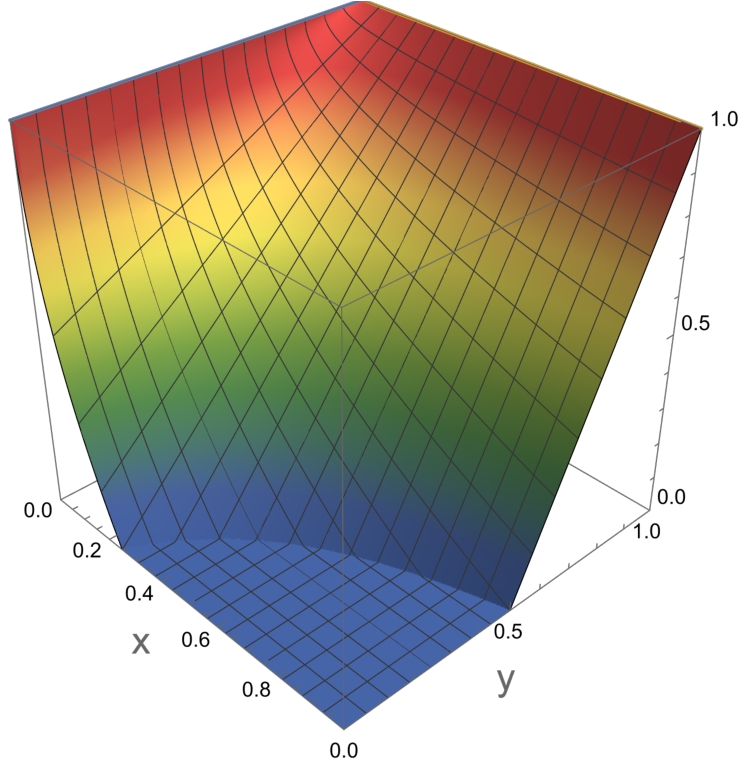
\includegraphics[width=5cm]{Ex2-1.pdf} }
		\subfloat[$I_2$]{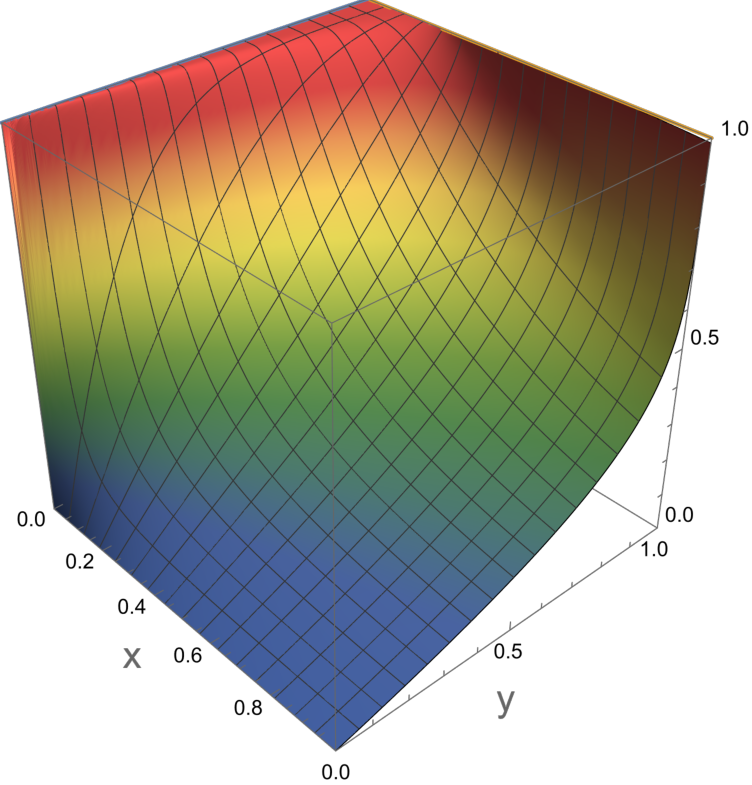
\includegraphics[width=5cm]{Ex2-2.pdf} }
		\caption[Plot of an $(f,e)$ and a $(g,e)$-implication]{Plot of fuzzy implication functions $I_{f_\lambda,e}$ and $I_{g_s,e}$ in Example \ref{example:2} with $e= \frac{1}{4}$ and $s=\lambda=2$.}\label{figure:example2}
	\end{figure}
\end{example}

At this point, we can rewrite Theorem \ref{ThmRepresentacio(h,e)} in terms of $(f,e)$ and $(g,e)$-implications using the definition of the horizontal threshold method (Theorem \ref{horizontalthreshold}) as follows.
\begin{corollary} Let $I:[0,1]^2 \to [0,1]$ be a binary function and $e \in (0,1)$. Then the following statements are equivalent:
	\begin{enumerate}[label=(\roman*)]
		\item $I$ is a generalized $(h,e)$-implication with respect to $e$, that is, $I=I^{h_g,e}$.
		\item There exists an $f$-generator and a $g$-generator with $g(1)=+\infty$ such that $I$ is given by $I=I_{I_{f,e} - I_{g,e}}$.
	\end{enumerate}
\end{corollary}

Then, in order to provide an axiomatic characterization of generalized $(h,e)$-implications based on this representation theorem, we need to study the two new families of fuzzy implication functions and provide their characterizations. Consequently, in this section we provide a further study of the properties of $(f,e)$ and $(g,e)$-implications, as particular cases of $(f,g)$ and $(g,f)$-implications. Moreover, we provide an axiomatic characterization of the two families thanks to the introduction of two new properties of fuzzy implication functions which are modifications of the standard law of importation \LI.

\subsection{Characterizations of $(f,e)$-generated implications}
In Section \ref{subsection:f-generated} we studied the additional properties of $(f,g)$-generated implications. Since $(f,e)$-generated implications are particular cases of $(f,g)$-generated implications, those results are also valid for $(f,e)$-implications. Thus, the first results of this section are corollaries which correspond to the properties of $(f,g)$-generated implications adapted to the particular case of $(f,e)$-implications. We only recall those properties that are relevant for solving the problem of the characterization of $(f,e)$-implications.

First of all, by Proposition \ref{onezonefg} we get that $(f,e)$-implications satisfy the lowest truth property, i.e., they have a trivial 1-region.

\begin{corollary}
	\label{onezone(f,e)} 
	Let $f$ be an $f$-generator and $e\in(0,1)$. Then $I_{f,e}(x,y)=1$ if and only if ($x=0$ or $y=1$).
\end{corollary}

Next, by Proposition \ref{prop:(f,g):(NP)} we recall that  $(f,e)$-generated implications do not fulfill the left neutrality principle \NP but we prove that they satisfy the modified version with $e\in(0,1)$. Observe that \NPe is also satisfied by generalized $(h,e)$-implications, strengthening the relation between the two families.

\begin{corollary} 
	Let $f$ be an $f$-generator  and $e\in(0,1)$. Then $I_{f,e}$ does not satisfy \NP, but it satisfies \NPe.
\end{corollary}
\begin{proof}
	Let be $f$ be an $f$-generator and $e \in (0,1)$. By Proposition \ref{prop:(f,g):(NP)} we obtain that $I_{f,e}$ does not satisfy \NP. On the other hand,
	$$I_{f,e}(e,x) = f^{(-1)}\left(\frac{e}{e}f(x)\right)=f^{(-1)} \circ f(x)=x, \quad \text{for all } x \in [0,1].$$
\end{proof}

Next, from Proposition \ref{negationfg} we get the expression of the natural negation of this family of fuzzy implication functions. As it will be proved later, this operator is important for characterizing $(f,e)$-implications.
\begin{corollary}
	Let $f$ be an $f$-generator and $e\in(0,1)$. The following properties hold:
	\begin{enumerate}[label=(\roman*)]
		\item If $f(0)=+\infty$, then the natural negation $N_{I_{f,e}}$ is the G\"odel or least negation $\NDOne$.
		\item If $f(0)<+\infty$, then the natural negation $N_{I_{f,e}}$ is given by
		$$N_{I_{f,e}}(x)=\left\{\begin{array}{ll} f^{-1}\left( \frac{x}{e}f(0)\right)&\hbox{if } x\leq e,\\ 0&\hbox{if } x>e.\end{array}\right.$$ 
	\end{enumerate}
	\label{negation}
\end{corollary}

Another important property of $(f,e)$-implications worthy to study is continuity, which depends on the value of the generator at zero (see Proposition \ref{prop:(f,g):continuity}).
\begin{corollary}
	\label{continuity(f,e)}
	Let $f$ be an $f$-generator  and $e\in(0,1)$. Then the following properties hold:
	\begin{enumerate}[label=(\roman*)]
		\item If $f(0)=+\infty$, then $I_{f,e}$ is continuous everywhere except at $(0,0)$.
		\item If $f(0)<+\infty$, then $I_{f,e}$ is continuous.
	\end{enumerate}
\end{corollary}

It is well known that \EP and \LI are two additional properties that are related, \LI being stronger than \EP. The following two results derived from Propositions \ref{EPfg} and \ref{prop:(f,g):(LI)} show that no $(f,e)$-implication satisfies the law of importation but, some of them satisfy the exchange principle.
\begin{corollary}
	Let $f$ be an $f$-generator and $e\in(0,1)$. Then $I_{f,e}$ satisfies \EP if and only if
	$f(0)=+\infty$.
\end{corollary}
\begin{corollary}
	Let $f$ be an $f$-generator and $e\in(0,1)$. Then $I_{f,e}$ does not satisfy \LI with any t-norm.
\end{corollary}
The last result reflects an important difference between Yager's implications and $(f,e)$-implications. It is well known that Yager's implications fulfill the law of importation \LI with respect to the product t-norm \TP. Moreover, this property plays a key role in the characterization of this family (see \cite{Massanet2012B}). Although $(f,e)$-implications do not fulfill the standard law of importation with respect to any t-norm, we prove that they satisfy two properties that resemble \LI. We provide the definition of these two new properties, which are two different modifications of the standard law of importation.

\begin{definition} 
	\label{novesli}
	A fuzzy implication function $I$ is said to satisfy
	\begin{enumerate}
		\item the \textit{$(x,ey)$-law of importation} with a t-norm $T$ for some $e \in(0,1]$, if
		$$
		I(T(x,y),z)= I(x,I(ey,z)) , \hbox{ for all } x,y,z \in [0,1].\eqno { \text{\LIey}} 
		$$
		\item the \textit{$(ex,y)$-law of importation} with a t-norm $T$ for some $e \in(0,1]$, if
		$$
		I(T(x,y),z)= I(ex,I(y,z)) , \hbox{ for all } x,y,z \in [0,1]. \eqno {\text{\LIex}}
		$$
	\end{enumerate}
\end{definition}

Notice that these two properties slightly modify the standard law of importation by limiting into $[0,e]$ the domain of one of the variables on the right-hand side of the equation. Clearly, we recover the standard law of importation when $e=1$. The motivation behind the introduction of these two properties is that we want to consider them in the characterizations of $(f,e)$-implications so they play a similar role to the one played by the standard law of importation in the characterization of Yager's implications.

The next proposition studies when the $(f,e)$-implications fulfill these two new properties. 

\begin{proposition}
	\label{LI_e(f,e)}
	Let $f$ be an $f$-generator  and $e\in(0,1)$. Then the following properties hold:
	\begin{enumerate}[label=(\roman*)]
		\item $I_{f,e}$ satisfies \LIey with respect to \TP.
		\item $I_{f,e}$ satisfies \LIex with respect to \TP if and only if $f(0)=+\infty$.
	\end{enumerate}
	\label{LIe}
\end{proposition}

\begin{proof}
	\begin{enumerate}[label=(\roman*)]
		\item On the one hand, we have
		$$I_{f,e}(xy,z)=f^{(-1)}\left(\frac{xy}{e}f(z)\right).$$
		On the other hand, we know that $f$ is strictly decreasing. Hence, for all $y,z \in [0,1]$ we get
		$$yf(z) \leq yf(0) \leq  f(0).$$
		Consequently,
		$$I_{f,e}(x,I_{f,e}(ey,z))= f^{(-1)}\left(\frac{x}{e} (f \circ f^{(-1)})(yf(z))\right) = f^{(-1)}\left(\frac{xy}{e}f(z)\right)$$
		and $I_{f,e}$ satisfies \LIey with respect to $\TP$.
		\item Let us assume that $f(0)=+\infty$. This implies that $f^{(-1)}=f^{-1}$ then, for all $x,y,z \in [0,1]$, we have
		$$I_{f,e}(ex,I_{f,e}(y,z))=f^{-1}\left(x (f\circ f^{-1})\left(\frac{y}{e}f(z)\right)\right)=f^{-1}\left(\frac{xy}{e}f(z)\right) = I_{f,e}(xy,z).$$
		Now, we assume that $f(0)< + \infty$. Consider $y,z \in [0,1]$ such that $yf(z)>ef(0)$ then we get
		$$ I_{f,e}(ex,I_{f,e}(y,z)) = f^{(-1)}\left(x (f \circ f^{(-1)})\left(\frac{y}{e}f(z)\right)\right) = f^{(-1)}(xf(0))=f^{-1}(xf(0)).$$
		Now, we can find some $x \in (0,1)$ small enough such that $xyf(z) \leq ef(0)$ and we have
		$$I_{f,e}(xy,z)=f^{(-1)}\left(\frac{xy}{e}f(z)\right) = f^{-1} \left( \frac{xy}{e}f(z)\right).$$
		Nevertheless, with the inequality $yf(z)>ef(0)$ and the strictly decreasing nature of $f^{-1}$, taking the previous considered $x \in (0,1)$ we get 
		$$ \frac{yf(z)}{e} > f(0) \Rightarrow \frac{xyf(z)}{e} > xf(0) \Rightarrow f^{-1}\left(\frac{xyf(z)}{e}\right) < f^{-1}(xf(0)).$$
		Consequently, $I_{f,e}(xy,z) \not = I_{f,e}(ex,I_{f,e}(y,z))$ and $I_{f,e}$ does not satisfy \LIex with respect to $\TP$.
	\end{enumerate}
\end{proof}

Observe that the two properties behave differently depending on the value $f(0)$. This is because of the presence of the pseudo-inverse of $f$ in the expression of these fuzzy implication functions. This fact results in the need to consider two different cases to provide the characterization of $(f,e)$-implication.


At this stage, using the preceding results we can present the characterization of $(f,e)$-generated implications with $f(0)<+\infty$.

\begin{theorem}\label{caractf0fin}
	Let $I:[0,1]^2\to [0,1]$ be a binary function and $e\in(0,1)$. Then the following statements are equivalent:
	\begin{enumerate}
		\item[(i)] $I$ is an $(f,e)$-generated implication with $f(0)<+\infty$.
		\item[(ii)] $I$ satisfies \LIey with $\TP$ and $N_I$ is a continuous fuzzy negation which is strictly decreasing in $(0,e)$ and such that $N_I(e)=0$.
	\end{enumerate}
	Moreover, in this case the $f$-generator is given by 
	\begin{equation}f(x)=N_{I}^{(-1)}(x)=\left\{\begin{array}{ll} N_I^{-1}(x)&\hbox{if } x >0,\\ e&\hbox{if } x=0.\end{array}\right.
		\label{GenFinites}
	\end{equation}
\end{theorem}

\begin{proof}
	Let $I$ be a binary function with $N_I$ a continuous fuzzy negation which is strictly decreasing in $(0,e)$ for some $e \in (0,1)$ such that $N_I(e)=0$ and satisfying \LIey with $\TP$. Let us define $f(x)=N_{I}^{(-1)}(x)$. First of all, we prove Equation (\ref{GenFinites}). Let us recall the definition of the pseudoinverse of a function
	$$N_I^{(-1)}(x) = \sup\{ z \in [0,1] ~,~ N_I(z)>x \}.$$
	Then, if $x=0$ we have
	$$N_I^{(-1)}(0)=\sup \{ z \in [0,1] ~,~ N_I(z)>0 \}=e.$$
	Otherwise, if $x>0$ as we know that $N_I$ is a bijection in $[0,e]$ and takes all the values in $[0,1]$ we obtain
	$$ N_I^{(-1)}(x)= \sup \{ z \in [0,1] ~|~ z < N_I^{-1}(x) \}=N_I^{-1}(x).$$
	Now, we see that $f$ is an $f$-generator. Since $N_I$ is a bijection in $[0,e]$ with $N_I(e)=0$, $f$ is continuous. Also, as $N_I$ is a strictly decreasing function in $[0,e]$, $f$ is strictly decreasing in $[0,1]$. In addition $f(0)=e < + \infty$ and $f(1)=N_I^{-1}(1)=0$. Now, we have
	$$ f^{-1}(x)= \left\{\begin{array}{ll} f^{-1}(x)&\hbox{if } x \in [0,f(0)],\\ 0&\hbox{if } x \in (f(0),1] ,\end{array}\right. = 
	\left\{\begin{array}{ll} N_I(x)&\hbox{if } x \in [0,e],\\ 0&\hbox{if } x \in (e,1] ,\end{array}\right.
	$$
	and then $f^{(-1)}(x)=N_I(x)$ for all $x \in [0,1]$. Finally, let us see that $I=I_{f,e}$. First, we develop the expression of $I_{f,e}$ with respect to the chosen $f$-generator. Using that $I$ satisfies \LIey with $\TP$ we get
	\begin{eqnarray*}
		I_{f,e}(x,N_I(y))&=&f^{(-1)}\left(\frac{x}{e}(f\circ f^{(-1)})(y)\right) =N_I\left(\frac{x}{e}(N_I^{(-1)} \circ N_I)(y)\right)\\
		&=& \left\{\begin{array}{ll} N_I\left(\frac{xy}{e}\right)&\hbox{if } N_I(y)>0,\\ N_I(x)&\hbox{if }N_I(y)=0 ,\end{array}\right. = \left\{\begin{array}{ll} 	I \left(\frac{xy}{e},0\right)&\hbox{if } y \in [0,e) ,\\ I(x,0) &\hbox{if }y\in [e,1] ,\end{array}\right. \\ 
		&=& \left\{\begin{array}{ll} 	I(x,I(y,0))&\hbox{if } y \in [0,e) ,\\ I(x,0) &\hbox{if }y\in [e,1] ,\end{array}\right. =
		\left\{\begin{array}{ll} 	I(x,N_I(y)) &\hbox{if } y \in [0,e) ,\\ I(x,N_I(y)) &\hbox{if }y\in [e,1] ,\end{array}\right.
	\end{eqnarray*}
	and we have that $ I_{f,e}(x,N_I(y)) = I(x,N_I(y))$ for all $y \in [0,1]$. Now, since $N_I$ takes all the values in $[0,1]$, the result follows.
	The reciprocal is guaranteed by (i)-Proposition \ref{LIe} and (ii)-Corollary \ref{negation}.
\end{proof}
\begin{remark} In order to show that the two properties considered in (ii)-Theorem \ref{caractf0fin} are independent from each other we provide the following two examples of fuzzy implication functions:
	$$I_1(x,y)= \left\{\begin{array}{ll} y^{2x}& \hbox{if } x>0 \hbox{ or } y>0,\\ 1&\hbox{if } x=0 \hbox{ and } y=0,\end{array}\right. \quad I_2(x,y)= \left\{\begin{array}{ll} 1-2x(1-y)& \hbox{if } x \in [0,0.5],\\ y&\hbox{if } x \in (0.5,1].\end{array}\right.$$
	If we consider $e=0.5$ it is easy to prove that $I_1$ satisfies \LIey with respect to $\TP$ but $N_{I_1}=\NDOne$ is not continuous. On the other hand, the natural negation of $I_2$ is the following
	$$N_{I_2}(x)=\left\{\begin{array}{ll} 1-2x& \hbox{if } x \in [0,0.5],\\ 0&\hbox{if } x \in (0.5,1].\end{array}\right.$$
	Thus, $N_{I_2}$ is continuous, strictly decreasing on $x \in [0,0.5]$ and $N_{I_2}(0.5)=0$ but $I_2$ does not satisfy \LIey with respect to $\TP$ since for $x=0.75$, $y=0.5$ and $z=0.5$ we have that
	$$I_2(\TP(0.75,0.5),0.5)=I_2(0.75 \cdot 0.5, 0.5)=0.625 < 0.75 =I_2(0.75, I_2(0.5 \cdot 0.5,0.5)).$$
\end{remark}

From this point on, we focus our attention to the case $f(0)=+\infty$. For providing the characterization of the remaining subfamily, we need to consider some other properties. First of all, we study the monotonicity of the horizontal and vertical sections of $(f,e)$-implications with  $f(0)=+\infty$.


\begin{lemma}\label{lema-previ}
	Let $f$ be an $f$-generator with $f(0)=+\infty$ and $e\in(0,1)$. Then the following properties hold:
	\begin{enumerate}[label=(\roman*)]
		\item The horizontal sections of $I_{f,e}$, $h_k(x)=I_{f,e}(x,k)$, are strictly decreasing for all $x\in[0,1]$ and $k\in(0,1)$.
		\item The vertical sections of $I_{f,e}$, $v_k(x)=I_{f,e}(k,x)$, are strictly increasing for all $x\in[0,1]$ and $k\in(0,1]$.
	\end{enumerate}
\end{lemma}

\begin{proof}
	\begin{enumerate}[label=(\roman*)]
		\item Let us assume $x_1,x_2\in [0,1]$ such that $x_1 < x_2$, then $\frac{x_1}{e}f(k) < \frac{x_2}{e}f(k)$. Now, since $f$ is strictly decreasing, $f^{-1}$ is also strictly decreasing and we get
		$$h_k(x_1)=I_{f,e}(x_1,k)=f^{-1}\left(\frac{x_1}{e} f(k)\right) > f^{-1} \left(\frac{x_2}{e}f(k)\right) = I_{f,e}(x_2,k)=h_k(x_2).$$
		
		Thus, the horizontal sections of $I_{f,e}$ are strictly decreasing for all $x \in [0,1]$ and $k\in (0,1)$.
		\item Let us assume $x_1,x_2 \in [0,1]$ such that $x_1<x_2$ then, since $f$ is strictly decreasing, we get that $\frac{k}{e}f(x_1) > \frac{k}{e}f(x_2)$ . Now because $f^{-1}$ is strictly decreasing we have
		$$v_k(x_1)=I_{f,e}(k,x_1)=f^{-1}\left(\frac{k}{e}f(x_1)\right) < f^{-1}\left(\frac{k}{e}f(x_2)\right) = I_{f,e}(k,x_2)=v_k(x_2)$$
		\noindent and the vertical sections of $I_{f,e}$ are strictly increasing for all $x\in [0,1]$ and $k \in (0,1]$.
	\end{enumerate}
\end{proof}


Before presenting the characterization of $(f,e)$-implications with $f(0)=+\infty$ we give some preliminary results. The following proposition emphasizes that the two new properties \LIey and \LIex with respect to $\TP$, in conjunction with the property that the binary operation equals $1$ if and only if ($x=0$ or $y=1$), and the continuity except at $(0,0)$, are crucial since they ensure that many other properties hold.

\begin{lemma}\label{lema-previ2} 
	Let $e\in(0,1)$ and $I:[0,1]^2\to [0,1]$ be a continuous function everywhere except at $(0,0)$ satisfying \LIey and \LIex with respect to $\TP$ and ($I(x,y)=1\Leftrightarrow x=0$ or $y=1$). Then the following properties hold:
	\begin{enumerate}[label=(\roman*)]
		\item $I(e,0)=0$.
		\item $I$ satisfies \NPe.
		\item The horizontal sections of $I$, $h_k:[0,1]\to[0,1]$ given by $h_k(x)=I(x,k)$, are strictly decreasing for all $k\in(0,1)$.
		\item $N_I=\NDOne$.
		\item The vertical sections of $I$, $v_k:[0,1]\to[0,1]$ given by $v_k(x)=I(k,x)$, are strictly increasing for all $k\in(0,1]$.
	\end{enumerate}
\end{lemma}

\begin{proof}
	\begin{enumerate}[label=(\roman*)]
		\item First of all we are going to prove that $I(e,0)=0$. On the contrary, let us suppose that $I(e,0)=a>0$ and let us get a contradiction.
		By \LIey for all $x \in [0,1]$ we get
		$$I(x,a)=I(x,I(e,0))=I(\TP(x,1),0)=I(x,0),$$
		and $N_I(x)=h_0(x)=h_a(x)$ is continuous since $h_a$ is. Now, since $I$ is continuous except at $(0,0)$ we get that all the horizontal sections of $I$ are continuous.\\
		Let us prove that the horizontal sections $h_k(x)$ are decreasing for all $k \in [0,1]$. For $k=1$ it is obvious since $h_1(x)=1$ for $x\in [0,1]$.  Otherwise, consider $x_1,x_2 \in [0,1]$ such that $x_1<x_2$ with $h_k(x_1)=h_k(x_2)$. If $h_k(x_1)=h_k(x_2)=1$ then $x_1=x_2=0$ and we get a contradiction. Then, let us assume $h_k(x_1)=h_k(x_2)<1$ with $0<x_1<x_2$ and by \LIex we get
		$$ I \left( \frac{ex_1}{x_2},h_k(x_2) \right) = I\left( \frac{ex_1}{x_2},I(x_2,k)\right) = I(x_1,k)=h_k(x_1)=h_k(x_2).$$
		Similarly, we obtain
		\begin{eqnarray*}
		 h_k(x_2) &=& I \left(\frac{ex_1}{x_2},h_k(x_2)\right) = I \left( \frac{ex_1}{x_2}, I\left( \frac{ex_1}{x_2},h_k(x_2)\right)\right) = I \left( e \left(\frac{x_1}{x_2}\right)^2,h_k(x_2) \right) \\
		 &=& I \left( e \left( \frac{x_1}{x_2}\right)^2, I(x_2,k)\right).
		 \end{eqnarray*}
		Consequently, if we iterate this process we obtain
		$$ I\left( e \left(\frac{x_1}{x_2}\right)^n , h_k(x_2)\right) = h_k(x_2),$$
		for all $n>0$. Now, if $h_k(x_2)=0$ we have
		$$ I \left( e \left(\frac{x_1}{x_2}\right)^n,a\right) = I \left( e \left(\frac{x_1}{x_2}\right)^n,0\right) =h_k(x_2)=0$$
		which is a contradiction since
		$$ \lim_{n\to+\infty}  I \left( e \left(\frac{x_1}{x_2}\right)^n,a\right) = I(0,a)=1>0.$$
		On the other hand, if $h_k(x_2)>0$ we have
		$$ h_k(x_2)=\lim_{n\to+\infty}  I \left( e \left(\frac{x_1}{x_2}\right)^n,h_k(x_2)\right) = I(0, h_k(x_2))=1 >h_k(x_2),$$
		and we also obtain a contradiction. Hence $h_k$ is injective and since $h_k(0)=I(0,k)=1$ we get that $h_k$ is decreasing and continuous for all $k \in [0,1]$. Besides, we also have that all the vertical sections are continuous since $v_0(x)= I(0,x)=1$ for all $x \in [0,1]$. Consequently, we get that $I$ is monotonic with respect to the first variable and continuous in each variable. Now by Theorem \ref{theorem:A04} we have that $I$ is, in fact, continuous so we get a contradiction.
		\item Consider $y \in (0,1)$. Since $v_e(x)$ is continuous with $v_{e}(0)=I(e,0)=0$ and $v_e(1)=1$ then there exists a $z\in (0,1)$ such that $v_e(z)=y$. Now, by \LIex we get
		$$I(e,y)=I(e,v_e(z))=I(e,I(e,z))=I(e,z)=v_e(z)=y.$$
		Also, $I(e,0)=0$ and $I(e,1)=1$. So $I$ satisfies \NPe.
		\item Consider $k \in (0,1)$ and let us prove that $h_k$ is injective considering three cases:
		\begin{itemize}
			\item  If $h_k(x_1)=h_k(x_2)=1$ then $x_1=x_2=0$.
			\item  If $0<h_k(x_1)=h_k(x_2)<1$ then necessarily $x_1,x_2>0$. Let us assume $x_1<x_2$,  by \LIex we get
			$$I \left( e\frac{x_1}{x_2}, h_k(x_2) \right) = I \left( e\frac{x_1}{x_2}, I(x_2,k) \right) = I(x_1,k)=h_k(x_1)=h_k(x_2).$$
			Consequently,
			$$ h_k(x_2) = I \left( e \frac{x_1}{x_2},h_k(x_2)\right) = I \left( e \frac{x_1}{x_2}, I \left( e \frac{x_1}{x_2}, h_k(x_2) \right) \right) = I \left( e \left(\frac{x_1}{x_2}\right)^2,h_k(x_2)\right).$$
			Following this idea we get
			$$I \left( e \left( \frac{x_1}{x_2}\right)^n,h_k(x_2) \right) = h_k(x_2),$$
			for all $n>0$. Since we have
			$$ h_k(x_2) = \lim_{n \to +\infty} I \left( e \left( \frac{x_1}{x_2}\right)^n,h_k(x_2)\right)=I(0,h_k(x_2))=1>h_k(x_2),$$
			we get a contradiction.
			\item  If $h_k(x_1)=h_k(x_2)=0$, let us assume $0 < x_1 \leq x_2$. We need to distinguish between two cases:
			\begin{itemize}
				\item  If $e> x_1$, since $h_k$ is continuous and $h_k(0)=I(0,k)=1$, there exists $x' \in (0,x_1)$ and $x^{*}\in(0,k)$ such that $h_k(x')=x^{*}$. Now, by (ii) we get that $h_k(e)=I(e,k)=k$ and there exists $x'' \in (x_1,e)$ with $h_k(x'')=x^{*}$ obtaining a contradiction as in the previous case. 
				\item  If $e \leq x_1 <x_2 \leq 1$ by \LIex we get that
				$$h_k(ex_1)=I(ex_1,k)=I(e^2,I(x_1,k))=I(e^2,h_k(x_1))=I(e^2,0),$$
				$$h_k(ex_2)=I(ex_2,k)=I(e^2,I(x_2,k))=I(e^2,h_k(x_2))=I(e^2,0),$$
				then $h_k(ex_1)=h_k(ex_2)<1$ with $ex_1 \leq ex_2 \leq e$. Now, if $h_k(ex_1)=h_k(ex_2)=0$ we get a contradiction as we have seen before and if $h_k(ex_1)=h_k(ex_2)>0$ then necessarily by a previous case $ex_1=ex_2$ and we get that $x_1=x_2$.
			\end{itemize}
		\end{itemize}
		Hence $h_k$ is injective and since $h_k(0)=I(0,k)=1$ we get that $h_k$ is strictly decreasing for all $k \in (0,1)$.
		\item First of all, let us see that $h_0(x)$ is decreasing for $x \in [0,1]$. Consider $0<x_1<x_2$ and a sequence $\{y_n\}_{n \geq 0}$ such that $y_n\in(0,1)$ and $y_n \rightarrow 0$. Then, using Point (iii) we get that
		$$h_{y_n}(x_1)=I(x_1,y_n)>I(x_2,y_n)=h_{y_n}(x_2),$$
		for all $n>0$. Then,
		$$I(x_1,0)=\lim_{n \to +\infty}I(x_1,y_n) \geq \lim_{n \to +\infty} I(x_2,y_n)=I(x_2,0).$$
		Now, we want to prove that $N_I=\NDOne$. We will see that $I(x,0)=0$ for all $x>0$. Let us assume that there exists $x_0>0$ such that $I(x_0,0)=a>0$. Then, for all $x\in(0,1)$, the sequence $\{x^n\}_{n \geq 0}$ is such that $x^n \to 0$ and by \LIex we have that
		$$ I(ex,a)=I(ex,I(x_0,0))=I(xx_0,0),$$
		$$I(ex^2,a)=I(ex,I(ex,a))=I(ex,I(xx_0,0))=I(x^2x_0,0).$$
		Consequently, for all $n>0$ we have that
		$$I(ex^n,a)=I(x^n x_0,0).$$
		Now, taking limits we get
		\begin{equation}
			\lim_{n \to +\infty} I(x^nx_0,0)=I(0,a)=1.
			\label{1}
		\end{equation}
		We will see that in this case we get a contradiction with the non-continuity of $I$ at the point $(0,0)$. Let $\{x_n\}_{n \geq 0}$ be a sequence such that $x_n>0$ and $x_n \to 0$ and $\varepsilon > 0$. By Equation (\ref{1}) there exists $n_0 \in \mathbb{N}$ such that for all $n \geq n_0$ we have that
		$$ I(x^{n}x_0,0)>1-\varepsilon.$$
		For this $n_0$ we have $x^{n_0}x_0>0$, and since $x_n \to 0$ there exists $n_1 \in \mathbb{N}$ such that $x_n \leq x^{n_0}x_0$ for all $n \geq n_1$. Then
		$$I(x_n,0) \geq I(x^{n_0}x_0,0) > 1-\varepsilon$$
		for all $n \geq n_1$. Now, we get that the sequence $\{I(x_n,0)\}_{n \geq 0}$ converges to 1 and we have that $h_0(x)$ is continuous in $x \in [0,1]$. Thus, we have a contradiction by the same argument used in Point (i). Hence, $N_I=\NDOne$.
		\item Consider $y_1 \leq y_2$ and $k \in (0,1)$ such that $v_k(y_1)=v_k(y_2)$, we will see that necessarily $y_1=y_2$ distinguishing three cases:
		\begin{itemize}
			\item  If $v_k(y_1)=v_k(y_2)=1$ then $y_1=y_2=1$.
			\item  If $v_k(y_1)=v_k(y_2)=0$ and $y_1=0$, $y_2>0$ we have two more cases:
			\begin{itemize}
				\item  If $k \in (e,1)$ then by Points (ii) and (iii) we get  $$v_k(y_1)=I(k,y_1) < I(e,y_1) =y_1=0$$
				which is a contradiction since the range of $v_k$ is $[0,1]$.
				\item  If $k \in (0,e]$ then again by Points (ii) and (iii) we have
				$$0=v_k(y_2)=I(k,y_2) \geq I(e,y_2)=y_2.$$
				Contradiction with the assumption $y_2>0$.
			\end{itemize}
			\item  If $0 \leq v_k(y_1)=v_k(y_2)<1$ and $0<y_1 \leq y_2$ then there exists an $x^{*} \in (0,1)$ such that $x^{*}<y_1 \leq y_2$ and we have that
			$$h_{x^{*}}(0)=I(0,x^{*})=1 ~,~ h_{x^{*}}(e)=I(e,x^{*})=x^{*}.$$
			Since the horizontal sections $h_k$ are continuous, there exist $x_1,x_2 \in (0,e)$ such that
			$$h_{x^*}(x_1)=I(x_1,x^{*})=y_1 ~,~ h_{x^*}(x_2)=I(x_2,x^{*})=y_2.$$
			Then, by \LIey we get
			\begin{eqnarray*}
			I\left(\frac{kx_1}{e},x^{*}\right) &=& I(k,I(x_1,x^{*}))=I(k,y_1) = I(k,y_2) \\
			&=& I(k,I(x_2,x^{*}))=I\left(\frac{kx_2}{e},x^{*}\right).
			\end{eqnarray*}
			Now, since the section $h_{x^*}$ is injective we get that
			$$\frac{kx_1}{e}=\frac{kx_2}{e} \Rightarrow x_1=x_2 \Rightarrow y_1=y_2.$$
		\end{itemize}
		Hence, the vertical sections $v_k$ are injective for $k \in (0,1)$. Now, since $v_k(1)=I(k,1)=1$ we get that $v_k$ are, in fact, strictly increasing for all $k \in (0,1)$.
	\end{enumerate}
\end{proof}

Observe that the above proposition uses the two variations of the law of importation. We remark that the property \LIex with respect to $\TP$ is not satisfied by $(f,e)$-generated implications with $f(0)<+\infty$, but it plays a capital role in the characterization of $(f,e)$-generated implications with $f(0)=+\infty$.

Lastly, we present the characterization of $(f,e)$-generated implications with $f(0)=+\infty$.

\begin{theorem}\label{caractf0inf}
	Let $I:[0,1]^2\to [0,1]$ be a binary function and $e\in(0,1)$. Then the following statements are equivalent:
	\begin{enumerate}
		\item[(i)] $I$ is an $(f,e)$-generated implication with $f(0)=+\infty$.
		\item[(ii)] $I$ satisfies \LIey and \LIex with respect to $\TP$, $I$ is continuous except at $(0,0)$ and ($I(x,y)=1 \Leftrightarrow x=0 \hbox{ or } y=1$). 
		\item[(iii)] $I$ satisfies \LIey and \LIex with respect to $\TP$, $N_I=\NDOne$, $I$ is continuous except at $(0,0)$ and there exists $k_0\in(0,1)$ such that 
		\begin{itemize}
			\item $h_k$ is strictly decreasing with $h_k(0)=1$ and $h_k(e)=k$ for all $k\in(0,k_0]$,
			\item $v_k$ are strictly increasing on the interval $[0,k_0]$ for all $k\in(0,1)$.
		\end{itemize}
		\item[(iv)] $I$ satisfies \LIey and \LIex with respect to $\TP$, $N_I=\NDOne$ and there exists $k\in(0,1)$ such that 
		\begin{itemize}
			\item $h_k$ is continuous and strictly decreasing with $h_k(0)=1$ and $h_k(e)=k$,
			\item $h_{\bullet}^{-1}(k):(0,k)\to[0,e]$ that assigns $h_y^{-1}(k)$ to some $y\in(0,k)$, is a well-defined, continuous and strictly increasing function satisfying 
			$\displaystyle \lim_{y\to 0^+}{h_y^{-1}(k)}=0$. 
		\end{itemize}
	\end{enumerate}
	Moreover, in this case the $f$-generator is given by
	\begin{equation}
		\label{fgen}
		f(x)=\left\{\begin{array}{ccl} \dfrac{h_k^{-1}(x)}{e} &\hbox{if }& k\leq x \leq 1,\\[1em] \dfrac{e}{h_x^{-1}(k)}&\hbox{if }& 0<x<k,\\[1em] +\infty &\hbox{if }& x=0.\end{array}\right.
	\end{equation}
\end{theorem}
\begin{proof}
	First, {\bf (i)$\Rightarrow$(ii)} is straightforward by Corollaries \ref{onezone(f,e)} and \ref{continuity(f,e)}  and Proposition \ref{LI_e(f,e)}.\\
	In order to prove that {\bf (ii)$\Rightarrow$(iii)} it is enough to use Lemma \ref{lema-previ2}.\\
	Let us prove {\bf(iii)$\Rightarrow$(iv)}. Consider $k=k_0$ then $h_k$ is continuous and strictly decreasing because $h_{k_0}$ is. Furthermore,
	$$h_k(0)=h_{k_0}(0)=1 ~,~ h_k(e)=h_{k_0}(e)=k=k_0.$$
	\begin{itemize}
		\item Let us prove that $h_{\bullet}^{-1}(k)$ is a well-defined function. Consider $y \in (0,k)$ then $h_y : [0,1] \to [h_y(1),1]$. Notice that $k\in [h_y(1),1]$ because we have that $h_y(0)=1$ and $h_y(e)=y$. Since $h_y$ is continuous and strictly decreasing there exists a unique $x_0 \in (0,1)$ such that $h_y(x_0)=I(x_0,y)=k$, then $h_y^{-1}(k)=x_0$.
		\item We will see that $h_{\bullet}^{-1}(k)$ is strictly increasing. Consider $0<y_1<y_2<k$, $x_1=h_{y_1}^{-1}(k)$ and $x_2=h_{y_2}^{-1}(k)$. Then by the fact that the vertical sections $v_{k'}$ are strictly increasing in $[0,k]$ for all $k' \in (0,1)$ we get that
		$$k=I(x_1,y_1)<I(x_1,y_2).$$
		Since $h_{y_2}$ is strictly decreasing we obtain that
		$$h_{y_2}(x_1)=I(x_1,y_2)>k = I(x_2,y_2)=h_{y_2}(x_2) \Rightarrow x_1 < x_2 \Rightarrow h_{y_1}^{-1}(k) < h_{y_2}^{-1}(k).$$
		\item Now, we prove that $h^{-1}_{\bullet}$ is continuous. Consider a decreasing sequence $\{y_n\}_{n \geq 0}$ with limit $y \in (0,k)$. We will see that the sequence $\{h^{-1}_{y_n}(k)\}_{n \geq 0}$ converges to $h_{y}^{-1}(k)$. Denote $x_n=h^{-1}_{y_n}(k)$ for all $n$ and let $x'$ be the limit of  $\{x_n\}_{n \geq 0}$, we know that this limit exists since $\{x_n\}_{n \geq 0}$ is bounded and strictly increasing. Now, since $I$ is continuous except at $(0,0)$ then $\{I(x_n,y_n)\}_{ n \geq 0}$ converges to $I(x',y)$. On the other hand, $I(x_n,y_n)=k$ for all $n$, then $I(x',y)=k$ and we get that $x' = h_y^{-1}(k)$. Therefore,
		$$\lim_{y_n \to y^{+}} h_{y_n}^{-1}(k)=h_y^{-1}(k).$$
		A similar argument taking an increasing sequence $\{y_n\}_{n \geq 0}$ such that $y_n \to y$ shows that
		$$ \lim_{y_n \to y^{-}} h_{y_n}^{-1}(k) =h_y^{-1}(k).$$
		Thus $h_y^{-1}(k)$ is continuous.
		\item Finally, we see that $\displaystyle \lim_{y \to 0^{+}} h_y^{-1}(k)=0$ for all $x \in [0,1]$ and $y \in (0,k)$. Consider a decreasing sequence $\{y_n\}_{n \geq 0}$ with $y_n \in (0,1)$ and $y_n \to 0$. Let $x'$ be the limit of $\{h_{y_n}^{-1}(k)\}_{n \geq 0}$. Let us assume that $x' \not = 0$, then $\{ I(h_{y_n}^{-1}(k),y_n) \}_{n \geq 0}$ converges to $I(x',0) = \NDOne(x)=0$. But we also have that $I(h^{-1}_{y_n}(k),y_n)=k$ for all $n>0$ and we get a contradiction.
	\end{itemize}
	Finally, let us prove that {\bf (iv)$\Rightarrow$(i)}. Consider the function $f$ given by Equation (\ref{fgen}) and let us prove that is an $f$-generator.
	\begin{itemize}
		\item Firstly, we will prove that $f$ is continuous and strictly decreasing. We see that $\frac{h_k^{-1}}{e}$ is continuous and strictly decreasing on the interval $[k,1]$ since $h_k$ is a continuous and strictly decreasing function. In addition $\frac{e}{h_{\bullet}^{-1}(k)}$ is also continuous and strictly decreasing since $h_x^{-1}(k) \not = 0$ for all $x \in (0,k)$ and $h_{\bullet}^{-1}(k)$ is strictly increasing. Finally, in order to see the continuity at $x=k$ we have that $ f(k)=\frac{h_k^{-1}(k)}{e}=\frac{e}{e}=1$ and
		$$\lim_{x \to k^{+}}f(x)=\lim_{x \to k } \frac{h_k^{-1}(x)}{e}= \frac{h_k^{-1}(k)}{e}=1,$$
		$$\lim_{x \to k^{-}}f(x)=\lim_{x \to k } \frac{e}{h_x^{-1}(k)}= \frac{e}{h_k^{-1}(k)}=1.$$
		\item $f(0)=+\infty$ by construction and $f(1)=\frac{h_k^{-1}(1)}{e}=0.$
	\end{itemize}
	Finally, we will prove that $I_{f,e}(x,y)=I(x,y)$ considering different cases:
	\begin{itemize}
		\item If $x \in [0,1]$ with $y \in [k,1]$ then there exists $z \in [0,e]$ such that $y=h_k(z)$ and we have
		$$I_{f,e}(x,y)=f^{-1}\left(\frac{x}{e}f(y)\right) = f^{-1} \left(\frac{x}{e}f(h_k(z))\right).$$
		Since $h_k(z) \in [h_k(e),h_k(0)]=[k,1]$ then we get
		$$I_{f,e}(x,y)=f^{-1}\left(\frac{xz}{e^2}\right).$$
		Now, we distinguish two subcases:
		\begin{itemize}
			\item If $xz \leq e^2$ then since $f^{-1}(w)=h_k(ew)$ for all $0 \leq w \leq 1$ and by \LIey we get
			$$ I_{f,e}(x,y) =h_k\left(\frac{xz}{e}\right) = I\left( \frac{xz}{e},k \right) = I(x,I(z,k))=I(x,y).$$
			\item If $xz > e^2$ then $f^{-1}\left(\frac{xz}{e^2}\right)=x'$ with $I\left(\frac{e^3}{xz},x'\right)=k$ . By \LIex, we get that
			$$I\left(\frac{e^3}{xz},I(x,y)\right)=I\left(\frac{e^2}{z},y\right) = I \left(\frac{e^2}{z},h_k(z)\right) = I\left(\frac{e^2}{z},I(z,k)\right)=I(e,k)=k.$$
			Now, since $h_{\bullet}^{-1}$ is strictly increasing we get
			$$I(x,y)=x'=I_{f,e}(x,y).$$
		\end{itemize}
		\item If $x \in [0,1]$ and $ y \in (0,k)$ we have
		$$I_{f,e}(x,y)=f^{-1}\left(\frac{x}{e}f(y)\right)=f^{-1}\left(\frac{x}{h_y^{-1}(k)}\right).$$
		Now, let us consider two more cases:
		\begin{itemize}
			\item If $ x \leq h_y^{-1}(k)$ then by \LIex we obtain that
			$$I_{f,e}(x,y)=h_k\left(\frac{ex}{h_y^{-1}(k)}\right) = I\left(\frac{ex}{h_y^{-1}(k)},k\right) = I\left(\frac{ex}{h_y^{-1}(k)}, I(h_y^{-1}(k),y)\right)=I(x,y).$$
			\item If $x> h_y^{-1}(k)$  then $f^{-1}\left(\frac{x}{h_y^{-1}(k)}\right)=x'$ such that $I\left(\frac{eh_y^{-1}(k)}{x},x'\right)=k$. Now, again by \LIex we have
			$$I \left(\frac{eh_y^{-1}(k)}{x},I(x,y)\right) = I(h_y^{-1}(k),y)=k,$$
			and again since $h_{\bullet}^{-1}$ is strictly increasing we  get that
			$$I(x,y)=x'=I_{f,e}(x,y).$$
		\end{itemize}
		\item Finally, if $x \in [0,1]$ and $y=0$ we have
		\begin{eqnarray*}
		I_{f,e}(x,0)&=&f^{-1}\left( \frac{x}{e} \cdot (+ \infty) \right)= \left\{ \begin{array}{ll}
			f^{-1}(0 \cdot (+\infty))=f^{-1}(0)=1 &   \text{if }   x=0, \\
			\\ f^{-1}\left(\frac{x}{e} \cdot (+\infty)\right)= f^{-1}(+\infty)=0 &\text{if } x>0,
		\end{array} \right. \\
		&=&\NDOne(x)=I(x,0).
		\end{eqnarray*} 
	\end{itemize}
\end{proof}
\begin{remark}\label{rmk2f}
	Recall that by Lemma \ref{lema-previ}, the horizontal sections $h_k$ and the vertical sections $v_k$ of an $(f,e)$-generated implication with $f(0)=+\infty$ are continuous and strictly decreasing or increasing, respectively, for all $k\in(0,1)$. Thus in fact any $k\in(0,1)$ can be used in order to obtain the $f$-generator through Equation (\ref{fgen}). 
\end{remark}

Notice that the previous characterization follows a similar structure to the one presented in \cite{Massanet2012B} for Yager's $f$-generated implications with $f(0)=+\infty$ using, in this case, the two modified laws of importation introduced in Definition \ref{novesli}.

In Table \ref{independence} we give some examples of functions $I:[0,1]^2\to[0,1]$ showing that none of the properties considered in (ii)-Theorem \ref{caractf0inf} is stronger than any of the others. More precisely, these examples show that none of the four properties in (ii)-Theorem \ref{caractf0inf}  can be directly deduced from one of the other properties. Perhaps the most remarkable result is that there exist binary operations in the unit interval which satisfy \LIex but do not satisfy \LIey and vice-versa. Note that these examples are not enough to ensure the independence of the four properties, to do such statement we should find binary operations which satisfy three of the properties and do not satisfy the excluding property, for each combination of cases. However, since \LIex and \LIey are two new properties in the literature, it is a difficult task to find such examples and a deeper study is needed. For instance, finding the function in the second row of Table \ref{independence} which satisfies \LIex but does not satisfy \LIey has been a challenging problem.

\begin{table}[t]
	\begin{center}
		\setlength\tabcolsep{7pt}
		\renewcommand{\arraystretch}{1.75} \large
		\begin{adjustbox}{max width=\textwidth}
			\begin{tabular}{|p{57mm}|M{30mm}|M{30mm}|M{30mm}|c|c|} \hline
				\centering \bf Function $I$  & \bf Fuzzy Impl. Funct.  & \LIey with $\TP$ for some $e \in (0,1)$ &\LIex with $\TP$ for some $e \in (0,1)$ &  \bf { $I(x,y)=1\Leftrightarrow$  $x=0$ or $y=1$} & \bf $I$ cont $\setminus\{(0,0)\}$ \\
				\hline
				$\left\{\begin{array}{ll} \dfrac{xy}{e}& \hbox{if } xy\leq e,\\ 1&\hbox{if } xy>e.\end{array}\right.$& \xmark & \cmark & \xmark & \xmark & \xmark\\
				\hline
				$\left\{ \begin{array}{ll}
					y^{\frac{x}{e}}  & \hbox{if }    x\ln(y) < -0.5e,\\
					1 &   \hbox{if }  x\ln(y) \geq -0.5e.
					
				\end{array}
				\right.$ & \cmark &\xmark & \cmark & \xmark & \xmark\\ \hline
				$\max\{1-x,y\}$ & \cmark &\xmark & \xmark & \cmark & \xmark\\ \hline
				$\left\{\begin{array}{ll} \dfrac{xy}{x^2+y^2}& \hbox{if } x,y>0,\\ 0&\hbox{if } x=y=0.\end{array}\right.$& \xmark &\xmark & \xmark & \xmark &\cmark \\ \hline
				$\left\{\begin{array}{ll} y^{x(1-y)}& \hbox{if } x>0 \hbox{ or } y>0,\\ 
					1&\hbox{if } x=y=0.\end{array}\right.$& \cmark &\xmark & \xmark & \cmark & \cmark \\ 
				\hline      
				$\left\{ \begin{array}{ll}
					1-\frac{x}{e} + \frac{xy}{e} &   \hbox{if }   y \geq 1-\frac{e}{x}, \\ 0  & \hbox{if }   y < 1-\frac{e}{x}.
				\end{array}
				\right.$ & \cmark &\cmark & \xmark & \cmark & \xmark\\ \hline
				
				$\left\{\begin{array}{ll} 1& \hbox{if } x=0 \hbox{ or } y=1 ,\\ 0& \hbox{otherwise}.\end{array}\right.$& \cmark &\cmark & \cmark & \cmark & \xmark\\ 
				\hline
				$\left\{ \begin{array}{lcc}
					y^{\frac{x}{e}} &   \hbox{if}  & x >0 \text{ or } y>0,         \\ 1  & \hbox{if}  & x=0 \text{ and } y=0.
				\end{array}
				\right.$ & \cmark &\cmark & \cmark & \cmark & \cmark\\
				\hline
			\end{tabular}
		\end{adjustbox}
	\end{center}
	\caption[Examples that prove that none of the additional properties in the characterization of $(f,e)$-implications with $f(0)=+\infty$ is stronger than any of the others.]{Some binary operations for which we have studied the four properties in (ii)-Theorem \ref{caractf0inf}.}\label{independence}
\end{table}

\subsection{Characterizations of $(g,e)$-generated implications}
The goal of this section is to characterize $(g,e)$-generated implications. In this case, since when $g(1) < +\infty$ the $(g,e)$-operation is not a fuzzy implication function, we only have the class of $(g,e)$-generated implications with $g(1)=+\infty$.

In order to characterize these fuzzy implication functions we will first study the intersection between $(f,e)$ and $(g,e)$-generated implications. Let us denote by
\begin{eqnarray*}
	\mathbb{I}_{\mathbb{F},e,\infty} &~-~& \text{the family of all } (f,e) \text{-generated implications with } f(0)=+ \infty;\\
	\mathbb{I}_{\mathbb{F},e,\aleph} &~-~& \text{the family of all } (f,e) \text{-generated implications with } f(0)<+ \infty;\\
	\mathbb{I}_{\mathbb{F},e} &=& \mathbb{I}_{\mathbb{F},e,\infty} \cup \mathbb{I}_{\mathbb{F},e,\aleph};\\
	\mathbb{I}_{\mathbb{G},e,\infty} &~-~& \text{the family of all } (g,e) \text{-generated implications with } g(1)=+ \infty.
\end{eqnarray*}
\noindent We have the following result.
\begin{proposition}
	$\mathbb{I}_{\mathbb{F},e,\infty} =\mathbb{I}_{\mathbb{G},e,\infty}$.
\end{proposition}
\begin{proof}
	Let us consider $I \in \mathbb{I}_{\mathbb{F},e,\infty}$, then there exists an $f$-generator $f$ with $f(0)=+ \infty$ and $I$ has the following form
	$$I(x,y)= f^{-1}\left(\frac{x}{e} f(y) \right), \hspace{0.5cm} x \in [0,1].$$
	Now, let us define a function $g:[0,1] \to [0,+ \infty]$ by
	$$g(x)=\frac{e}{f(x)}, \hspace{0.5cm} x \in [0,1],$$
	\noindent with the assumptions $\frac{1}{0}=+\infty$ and $ \frac{1}{+ \infty}=0$. Notice that $g$ is a $g$-generator with $g(1)=+\infty$. Moreover $g^{(-1)}(x)=g^{-1}(x)=f^{-1}(\frac{e}{x})$. Hence, for all $x,y \in [0,1]$, we have that
	$$I_{g,e}(x,y)=g^{-1}\left(\frac{e}{x}g(y)\right)=g^{-1}\left(\frac{e^2}{x}\frac{1}{f(y)}\right) = f^{-1}\left(\frac{x}{e}f(y)\right)=I(x,y).$$
	Conversely, if $I \in \mathbb{I}_{\mathbb{G},e,\infty}$ then there exists a $g$-generator with $g(1)=+ \infty$ with which $I$ has the following form
	$$I(x,y) = g^{-1}\left(\frac{e}{x}g(y)\right), \hspace{0.5cm} x,y \in [0,1].$$
	Now, we define a function $f:[0,1] \to [0,+\infty]$ by
	$$f(x)=\frac{1}{eg(x)}, \hspace{0.5cm} x \in [0,1],$$ 
	\noindent with the same assumptions as before. Then $f$ is an $f$-generator with $f(0)= + \infty$ and $f^{(-1)}(x)=f^{-1}(x)=g^{-1}(\frac{1}{ex})$. Now, for every $x,y \in [0,1]$ we get
	$$I_{f,e}(x,y) =f^{-1}\left(\frac{x}{e}f(y)\right) = f^{-1}\left(\frac{x}{e^2}\frac{1}{g(y)}\right)=g^{-1}\left(\frac{e}{x}g(y)\right)=I(x,y).$$
\end{proof}

In the proof of the last result we see the relationship between the $g$-generators with $g(1)=+\infty$ and $f$-generators with $f(0)=+\infty$. Specifically, given an $f$-generator with $f(0)=+\infty$ then the function
$$g(x)=\frac{1}{ef(x)}, \quad \text{for all } x \in [0,1],$$
is a $g$-generator with $g(1)=+\infty$. Consequently, the following characterization of $(g,e)$-implications can be directly deduced from Theorem \ref{caractf0inf}.

\begin{theorem}\label{caractg1fin}
	Let $I:[0,1]^2\to [0,1]$ be a binary function and $e\in(0,1)$. Then the following statements are equivalent:
	\begin{enumerate}
		\item[(i)] $I$ is a $(g,e)$-generated implication with $g(1)=+\infty$.
		\item[(ii)] $I$ satisfies \LIey and \LIex with respect to $\TP$, $I$ is continuous except at $(0,0)$ and ($I(x,y)=1 \Leftrightarrow x=0 \hbox{ or } y=1$). 
		\item[(iii)] $I$ satisfies \LIey and \LIex with respect to $\TP$, $N_I=\NDOne$, $I$ is continuous except at $(0,0)$ and there exists $k_0\in(0,1)$ such that 
		\begin{itemize}
			\item $h_k$ is strictly decreasing with $h_k(0)=1$ and $h_k(e)=k$ for all $k\in(0,k_0]$,
			\item $v_k$ are strictly increasing on the interval $[0,k_0]$ for all $k\in(0,1)$.
		\end{itemize}
		\item[(iv)] $I$ satisfies\LIey and \LIex with respect to $\TP$, $N_I=\NDOne$ and there exists $k\in(0,1)$ such that 
		\begin{itemize}
			\item $h_k$ is continuous and strictly decreasing with $h_k(0)=1$ and $h_k(e)=k$,
			\item $h_{\bullet}^{-1}(k):(0,k)\to[0,e]$ that assigns $h_y^{-1}(k)$ to some $y\in(0,k)$, is a well-defined, continuous and strictly increasing function satisfying 
			$\displaystyle \lim_{y\to 0^+}{h_y^{-1}(k)}=0$. 
		\end{itemize}
	\end{enumerate}
	Moreover, in this case the $g$-generator is given by
	\begin{equation}
		\label{ggen}
		g(x)=\left\{\begin{array}{ccl} \dfrac{1}{h_k^{-1}(x)} &\hbox{ if }& k\leq x \leq 1,\\[1em] \dfrac{h_x^{-1}(k)}{e^2}&\hbox{ if }& 0<x<k,\\[1em] 0 &\hbox{ if }& x=0.\end{array}\right.
	\end{equation}
\end{theorem}

\section{Representations of $(f,e)$ and $(g,e)$-implications}\label{section:representation(f,e)}

In \cite{Vemuri2014} equivalence classes on the set $\mathbb{I}$ of all fuzzy implication functions were defined in order to obtain representations of the families of Yager's $f$ and $g$-generated implications. Along this section, we present an analogous argument with the aim of obtaining representations of the two new families introduced in this chapter, the $(f,e)$ and $(g,e)$-implications.\\


First, let us introduce the definition of a $\varphi$-pseudo conjugate of a fuzzy implication function. We denote by $\Phi$ the family of all increasing bijections from $[0,1]$ to $[0,1]$.

\begin{definition}[\textbf{\cite[Definition 4.7]{Vemuri2014}}] If $I$,$J \in \mathbb{I}$ are related as $J(x,y) = \varphi ( I (x, \varphi^{-1}(y)))$ for all $x,y \in [0,1]$ for some $\varphi \in \Phi$, we say that $J$ is a $\varphi$-pseudo conjugate of $I$, or equivalently, $I$ is a $\varphi^{-1}$-pseudo conjugate of $J$.
\end{definition}

Thanks to the last definition, we are able to define in a simple way the equivalence classes on the set $\mathbb{I}$ based on the pseudo-conjugacy of fuzzy implication functions.

\begin{definition}[\textbf{\cite[Remark 4.6]{Vemuri2014}}]
	If $I \in \mathbb{I}$, the equivalence class containing $I$ can be given by
	$$ [I] = \{ J \in \mathbb{I} ~|~ J \text{ is a } \varphi\text{-pseudo conjugate of } I \}.$$
\end{definition}
\begin{remark} Since an $(f,e)$-implication is a particular case of an $(f,g)$-implication, if $f$ is an $f$-generator such that $f(0)<+\infty$, then the function $f_1:[0,1] \to [0,1]$ defined by
	$$ f_1(x)=\frac{f(x)}{f(0)}, \hspace{0.5cm} x\in[0,1],$$
	is a well-defined $f$-generator such that $f(0)=1$ and $I_{f,e} = I_{f_1,e}$. Then, if $\mathbb{I}_{\mathbb{F},e,1}$ is the set of all $(f,e)$-implications with $f(0)=1$, we have that $\mathbb{I}_{\mathbb{F},e,1}=\mathbb{I}_{\mathbb{F},e,\aleph}$.
\end{remark}
\begin{remark}[\textbf{\cite[Remark 5.3]{Vemuri2014}}] Note that for every $f$-generator $f$, the function $ f \circ \varphi : [0,1] \to [0, +\infty]$ is strictly decreasing and $(f \circ \varphi)(1)=0$ for all $ \varphi \in \Phi$. Thus $f \circ \varphi$ is also an $f$-generator for every $\varphi \in \Phi$.
\end{remark}

The first result shows that if $I$ is an $(f,e)$-implication then any $\varphi$-pseudo conjugate of $I$ is also an $(f,e)$-implication.

\begin{lemma} Let $I\in \mathbb{I}$ and $J \in [I]$. Then $ I \in \mathbb{I}_{\mathbb{F},e} \Leftrightarrow J \in \mathbb{I}_{\mathbb{F},e}$.
	\label{lemclaseqIfe}
\end{lemma}
\begin{proof}
	Let $I\in \mathbb{I}_{\mathbb{F},e}$ and $J \in [I]$. Then $I(x,y)=f^{(-1)}(\frac{x}{e}f(y))$ for some $f$-generator $f$. Now, we have that
	\begin{eqnarray*}
	J(x,y) &=& \varphi (I(x,\varphi^{-1}(y)) = \varphi \left(f^{(-1)}\left(\frac{x}{e} f ( \varphi^{-1}(y))\right) \right) \\
	&=& (f \circ \varphi^{-1})^{(-1)}\left(\frac{x}{e}(f \circ \varphi^{-1})(y)\right) = I_{f \circ \varphi^{-1},e}(x,y).
	\end{eqnarray*}
	Then $J$ is an $(f,e)$-implication. The converse can be proved analogously.
\end{proof} 

The next result shows that the previous lemma can be stronger in the sense that it is also true for the two subfamilies considered of $(f,e)$-implications.

\begin{lemma} Let $I \in \mathbb{I}$ and $J \in [I]$. Then the following statements hold:
	\begin{enumerate}[label=(\roman*)]
		\item $I \in \mathbb{I}_{\mathbb{F},e,\infty} \Leftrightarrow J \in \mathbb{I}_{\mathbb{F},e,\infty}$.
		\item $I \in \mathbb{I}_{\mathbb{F},e,1} \Leftrightarrow J \in \mathbb{I}_{\mathbb{F},e,1}$.
	\end{enumerate}
	\label{lemaclas}
\end{lemma}
\begin{proof}
	Let $I$ be an $(f,e)$-implication and $J \in [I]$. From Lemma \ref{lemclaseqIfe} we know that $J=I_{f \circ \varphi^{-1},e}$ for some $\varphi \in \Phi$. Since $ f \circ \varphi^{-1}$ is an $f$-generator and
	$$(f \circ \varphi^{-1})(0)=f(\varphi^{-1}(0))=f(0),$$
	\noindent then the result follows.
\end{proof}


As we have already mentioned, in \cite{Vemuri2014} a representation for the family of generated $f$-implications based on these equivalence classes was presented. Specifically, it was proved that the set of all $f$-generated implications is equal to $[\IYG]\cup [\IRC]$. In our case, we prove a similar result for the $(f,e)$-implications choosing different representatives for the classes. For this purpose we consider the $(f,e)$-implications related to the $f$-generators $f_1(x)=-\ln x$ and $f_2(x)=1-x$ for all $x \in [0,1]$ given by
$$I_{\bf YG}^e(x,y)= \left\{ \begin{array}{lcc}
	y^{\frac{x}{e}} &   \hbox{if}  & x >0 \text{ or } y>0,         \\ 1  & \hbox{if}  & x=0 \text{ and } y=0,
\end{array}
\right.
\hspace{0.5cm}
I_{\bf RC}^e(x,y)= \left\{ \begin{array}{lcc}
	1-\frac{x}{e} + \frac{xy}{e} &   \hbox{if}  & y \geq 1-\frac{e}{x}, \\ 0  & \hbox{if}  & y < 1-\frac{e}{x}.
\end{array}
\right.
$$
Now, we prove that every $(f,e)$-implication is a a $\varphi$-pseudo conjugate of either $I_{\bf YG}^e$ or $I_{\bf RC}^e$.
\begin{theorem} $\mathbb{I}_{\mathbb{F},e,\infty} = [I_{\bf YG}^e]$.
\end{theorem}

\begin{proof}
	We know by construction that $I_{\bf YG}^e \in \mathbb{I}_{\mathbb{F},e,\infty}$. Now, by (i)-Lemma \ref{lemaclas} if $J \in [I_{\bf YG}^e]$ then $J \in \mathbb{I}_{\mathbb{F},e,\infty}$ and consequently $[I_{\bf YG}^e]\subseteq \mathbb{I}_{\mathbb{F},e,\infty}$.
	On the other hand, let $I \in \mathbb{I}_{\mathbb{F},e,\infty}$  then $I=I_{f,e}$ for some $f$-generator with $f(0)=+\infty$. Let us take $\varphi(x)=f^{-1}(-\ln x)$, then $\varphi(0)=0$ and $\varphi(1)=1$. Furthermore, $\varphi$ is  an increasing bijection on $[0,1]$ and hence $\varphi \in \Phi$. Now, if we consider $f_1(x)=-\ln x$ we have that
	$$(f_1 \circ \varphi^{-1})(x)=f_1(e^{-f(x)})=- \ln ( e^{-f(x)})=f(x),$$
	\noindent thus $I=I_{f,e}=I_{f_1 \circ \varphi^{-1},e}$. Then, $I \in [I_{\bf YG}^e]$ and therefore, $ \mathbb{I}_{\mathbb{F},e,\infty} \subseteq [I_{\bf YG}^e]$.
\end{proof}

\begin{theorem} $\mathbb{I}_{\mathbb{F},e,1} = [I_{\bf RC}^e]$.
\end{theorem}
\begin{proof}
	We know that $I_{\bf RC}^e$ is an $(f,e)$-implication with the $f$-generator $f(x)=1-x$. Since $f(0)=1 < + \infty$ then $I_{\bf RC}^e \in \mathbb{I}_{\mathbb{F},e,1}$. Now, let us consider $J \in [I_{\bf RC}^e]$, then from (ii)-Lemma \ref{lemaclas} it follows that $J \in \mathbb{I}_{\mathbb{F},e,1}$ and we have $[I_{\bf RC}^e] \subseteq \mathbb{I}_{\mathbb{F},e,1}$. On the other hand, if $I \in \mathbb{I}_{\mathbb{F},e,1}$ then $I=I_{f,e}$ for some $f$-generator $f$ with $f(0) = 1$. Let us consider $\varphi(x)=f^{-1}(1-x)$. It is straightforward that $\varphi(0)=0$, $\varphi(1)=1$ and $\varphi(x)$ is an increasing bijection on $[0,1]$. Now, if we take $f_2(x)=1-x$ then we have that
	$$(f_2 \circ \varphi^{-1})(x)=f_2(1-f(x))=f(x)$$
	thus $I=I_{f,e}=I_{f_2 \circ \varphi^{-1}}$ and we get that $I \in [I_{\bf RC}^e]$.
\end{proof}


\begin{remark} Since $\mathbb{I}_{\mathbb{F},e,\infty} = \mathbb{I}_{\mathbb{G},e,\infty}$, it is straightforward that $\mathbb{I}_{\mathbb{G},e,\infty} = [I_{\bf YG}^e]$. Then, we have also obtained a representation for the $(g,e)$-implications.
\end{remark}

\begin{example} In Figure \ref{(f,e)conj} we can see the plot of the function $I_{\bf RC}^e$ with respect to $e=\frac{1}{4}$ jointly with two of their pseudo-conjugates, which we know that are also $(f,e)$-implications with respect to an $f$-generator with $f(0)<+\infty$. Notice that the natural negations of these fuzzy implication functions are strictly decreasing in $[0, \frac{1}{4}]$ with $N\left(\frac{1}{4}\right)=0$, fact that is straightforward from the characterization of $(f,e)$-implications when $f(0)<+\infty$ (Theorem \ref{caractf0fin}).
	\begin{figure}[t]
		\centering
		\subfloat[$I_{\bf RC}^{\frac{1}{4}}$]{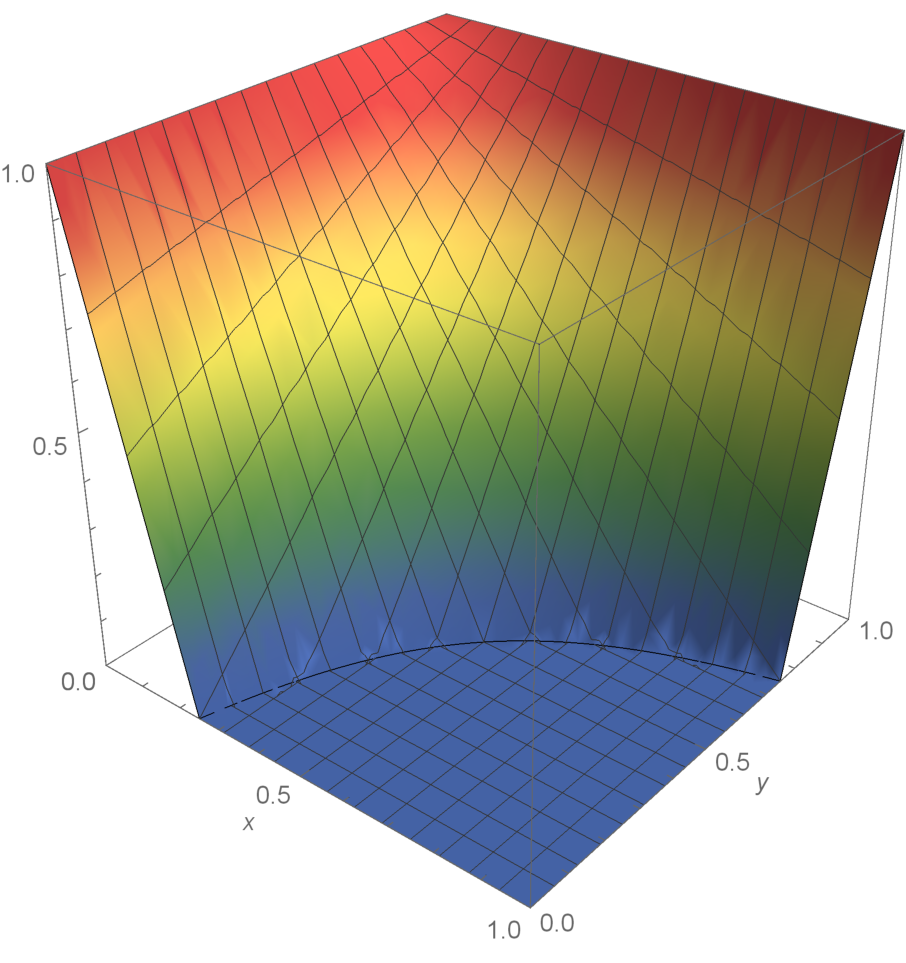
\includegraphics[width=4cm]{c1.pdf} } \quad
		\subfloat[$(I_{\bf RC}^{\frac{1}{4}})_{\varphi}$ with $\varphi(x)=x^2$]{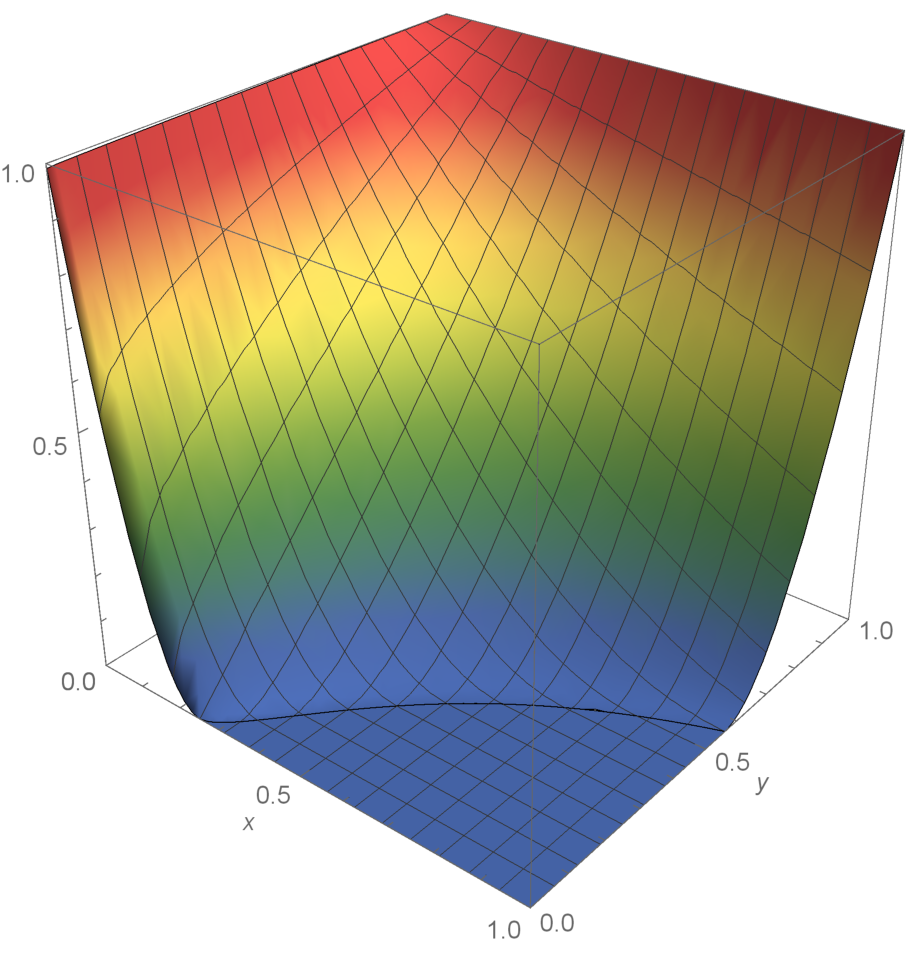
\includegraphics[width=4cm]{c2.pdf} } \quad
		\subfloat[$(I_{\bf RC}^{\frac{1}{4}})_{\varphi}$ with $\varphi(x)=\sqrt{x}$]{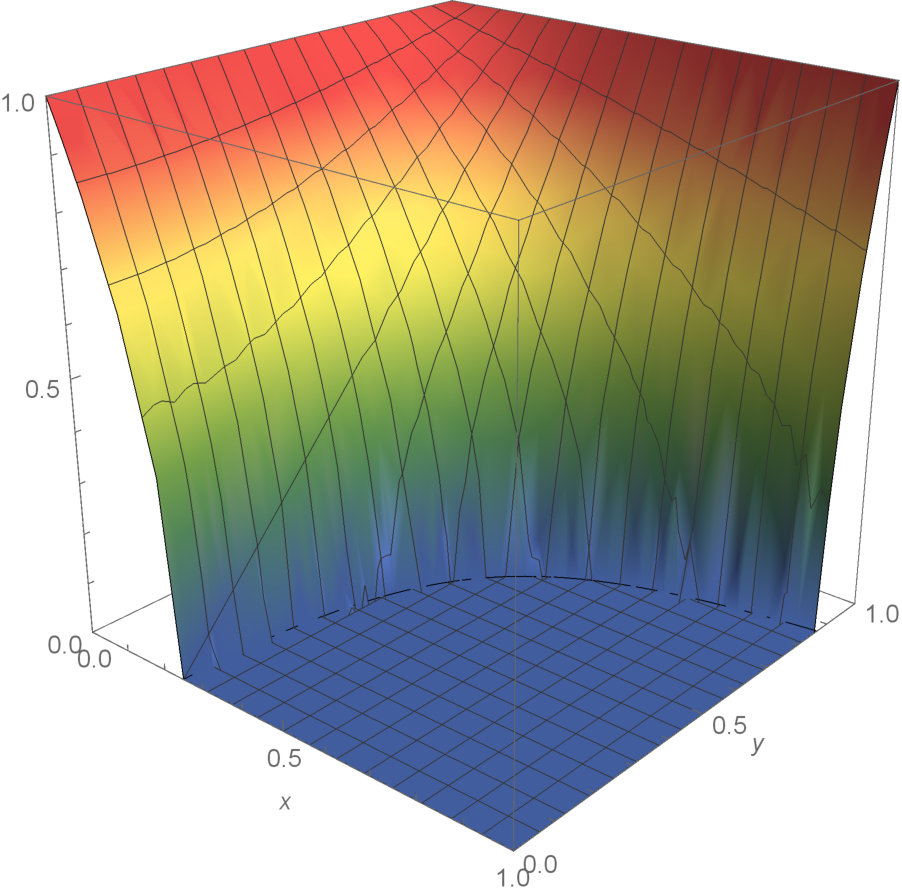
\includegraphics[width=4cm]{c3.pdf} }\\
		\caption{Plot of the fuzzy implication function $I_{\bf RC}^e$ with $e=\frac{1}{4}$ jointly with two of its $\varphi$-pseudo conjugates.}\label{(f,e)conj}
	\end{figure}
\end{example}

\section{Characterizations of generalized $(h,e)$-implications}\label{section:characterization(h,e)}

In this section we use the representation theorem of generalized $(h,e)$-implications and the characterizations of $(f,e)$ and $(g,e)$-implications presented in Section \ref{section:characterizations(f,e)&(g,e)} in order to provide an axiomatic characterization for generalized $(h,e)$-implications.

The idea of the proofs is to translate the properties that appear in the characterizations of the $(f,e)$ and $(g,e)$-implications to properties related to generalized $(h,e)$-implications by using the representation theorem of this family. We have seen that the characterization of $(f,e)$-implications is significantly different when $f(0)$ is finite or not. For this reason, we distinguish two cases also for the characterization of generalized $(h,e)$-implications.

First of all, we need to study when the generalized $(h,e)$-implications satisfy the new properties of fuzzy implication functions introduced in this work, \LIex and \LIey with respect to the product t-norm $\TP$.

\begin{proposition} Let $h$ be a generalized $h$-generator and $e \in (0,1)$. Then
	
	\begin{enumerate}[label=(\roman*)]
		\item $I^{h_g,e}$ satisfies \LIey with respect to $\TP$.
		\item It holds that $I^{h_g,e}(xy,z)=I^{h_g,e}(ex,I^{h_g,e}(y,z))$ for all $x,y \in [0,1]$ and $z \in [e,1]$.
		\item $I^{h_g,e}$ satisfies \LIex with respect to $\TP$ if and only if $h(0)=-\infty$.
	\end{enumerate}
	\label{propietats2(h,e)}
\end{proposition}
\begin{proof} Let us consider $e\in (0,1)$, $I$ a generalized $(h,e)$-implication and $h$ a generator of $I$.
	\begin{enumerate}[label=(\roman*)] 
		\item On the one hand,
		$$I(xy,z)= \left\{ \begin{array}{lcl}
			1 &   \hbox{if}  & x=0 \hbox{ or } y=0, \\
			h^{(-1)}\left( \frac{xy}{e}h(z) \right) &   \hbox{if}  & x,y>0 \hbox{ and } z \leq e, \\
			h^{-1}\left( \frac{e}{xy}h(z) \right) &   \hbox{if}  & x,y>0 \hbox{ and } z > e. \\
		\end{array}
		\right.
		$$
		Now, in order to prove the equality $I(xy,z)=I(x,I(ey,z))$ let us distinguish different cases:
		\begin{itemize}
			\item If $x=0$ we have that
			$$I(0,z)=1=I(0,I(ey,z)), \hspace{0.5cm} \text{ for all } y,z \in [0,1].$$
			\item If $y=0$ it holds that
			$$I(0,z)=1=I(x,1)=I(x,I(0,z)), \hspace{0.5cm} \text{ for all } y,z \in [0,1].$$
			\item If $x,y>0$ and $z \leq e$ then
			$$I(x,I(ey,z))=I(x,h^{(-1)}(yh(z))).$$
			We have that $yh(z) \geq h(z) > h(0)$ and consequently $h^{(-1)}(yh(z))=h^{-1}(yh(z))$. Moreover, since $h$ is strictly increasing, $h^{-1}$ is increasing in $(h(0),0]$ and 
			$$h(z) \leq h(e)=0 \Rightarrow yh(z) \leq 0 \Rightarrow h^{-1}(yh(z)) \leq h^{-1}(0)=e.$$
			Thus,
			\begin{eqnarray*}
			I(x,I(ey,z)) &=& I(x,h^{-1}(yh(z))) = h^{(-1)} \left( \frac{x}{e}(h \circ h^{-1})(yh(z))\right) \\
			&=& h^{(-1)} \left( \frac{xy}{e}h(z)\right) = I(xy,z).
			\end{eqnarray*}
			\item If $x,y>0$ and $z>e$ then
			$$I(x,I(ey,z))=I\left(x,h^{-1}\left(\frac{h(z)}{y}\right)\right).$$
			Again, by the strictly increasing nature of $h$, $h^{-1}$ is strictly increasing in $(0,+\infty)$ and then
			$$ \frac{1}{y} \geq 1 \Rightarrow \frac{h(z)}{y} \geq h(z) > h(e)=0 \Rightarrow h^{-1} \left( \frac{h(z)}{y}\right) > h^{-1}(0)=e.$$
			Hence,
			\begin{eqnarray*}
			I(x,I(ey,z))&=&I\left(x,h^{-1}\left(\frac{h(z)}{y}\right)\right) = h^{-1}\left(\frac{e}{x}(h \circ h^{-1})\left(\frac{h(z)}{y}\right)\right)\\
			&=&I\left(\frac{e}{xy}h(z)\right)=I(xy,z).
			\end{eqnarray*}
		\end{itemize}
		\item We have to prove that $I(xy,z)=I(ex,I(y,z))$ for all $x,y\in [0,1]$ and $z\geq e$.
		\begin{itemize}
			\item If $x=0$ we have that
			$$I(0,z)=1=I(0,I(y,z)), \hspace{0.5cm} \text{ for all } y,z \in [0,1].$$
			\item If $y=0$ it holds that
			$$I(0,z)=1=I(ex,1)=I(ex,I(0,z)), \hspace{0.5cm} \text{ for all } y,z \in [0,1].$$
			\item If $x,y>0$ and $z=e$ then since $h(e)=0$ we have that
			$$I(ex,I(y,e))=I\left(ex,h^{(-1)}\left(\frac{y}{e}h(e)\right)\right) = I(ex,e)=h^{(-1)}(xh(e))=e.$$
			On the other hand, $I(xy,e)=h^{(-1)}\left(\frac{xy}{e}h(e)\right)=e$.
			\item If $x,y>0$ and $z>e$ then
			$$I(ex,I(y,z)) = I\left(ex, h^{-1} \left(\frac{e}{y}h(z)\right)\right).$$
			Now, since $h$ is strictly increasing, $h^{-1}$ is strictly increasing in $(0,+\infty)$ and we get that
			$$\frac{e}{y} \geq e \Rightarrow \frac{e}{y}h(z) \geq eh(z) > eh(e) =0 \Rightarrow h^{-1}\left(\frac{e}{y}h(z)\right) > h^{-1}(0)=e,$$
			and then
			\begin{eqnarray*}
			I(ex,I(y,z)) &=& I\left(ex, h^{-1} \left(\frac{e}{y}h(z)\right)\right) = I\left(\frac{1}{x}(h \circ h^{-1})\left(\frac{e}{y}h(z)\right)\right) \\
			&=& I\left(\frac{e}{xy}h(z)\right)=I(xy,z).
			\end{eqnarray*}
		\end{itemize}
		\item First, let $h$ be a generalized $h$-generator with $h(0) > -\infty$. Let us consider $x \in (0,1)$, $y \in (0,1]$ and $z \in [0,e)$ such that $yh(z) < eh(0)$, then
		$$I(ex,I(y,z))=I\left(ex,h^{(-1)}\left(\frac{y}{e}h(z)\right)\right) = I(ex,0)=h^{(-1)}(xh(0))=h^{-1}(xh(0)).$$
		On the other hand, we can find an $x\in(0,1)$ small enough such that $xyh(z)>eh(0)$ and we get that
		$$I(xy,z)=h^{(-1)}\left(\frac{xy}{e}h(z)\right)=h^{-1}\left(\frac{xy}{e}h(z)\right).$$
		But since $h^{-1}$ is strictly increasing in $[h(0),0)$ we have that
		$$\frac{yh(z)}{e} < h(0) \Rightarrow \frac{xyh(z)}{e} <xh(0) \Rightarrow h^{-1}\left(\frac{xyh(z)}{e}\right) < h^{-1}(xh(0)).$$
		Thus, $I$ does not satisfy \LIex with respect to $\TP$. On the other hand, consider $h$ a generalized $h$-generator with $h(0)=-\infty$, then $h^{(-1)}=h^{-1}$. Considering Point (ii), we only need to prove that $I$ satisfies $I(xy,z)=I(ex,I(y,z))$ for all $x,y\in[0,1]$ and $z \in [0,e)$. First
		$$I(ex,I(y,z))= I\left(ex,h^{-1}\left(\frac{y}{e}h(z)\right)\right).$$
		Now, since $\frac{y}{e}h(z) \leq 0$, we have that $h^{-1}\left(\frac{y}{e}h(z)\right) \leq h^{-1}(0)=e$ due to the increasingness of $h^{-1}$. Thus,
		\begin{eqnarray*}
		I(ex,I(y,z)) &=& I\left(ex,h^{-1}\left(\frac{y}{e}h(z)\right)\right) = h^{-1}\left(x (h \circ h^{-1})\left(\frac{y}{e}h(z)\right)\right)\\
		&=&h^{-1}\left(\frac{xy}{e}h(z)\right)=I(xy,z).
		\end{eqnarray*}
	\end{enumerate}
\end{proof}

At this point and using the previous results, we can obtain the characterization of generalized $(h,e)$-implications in both cases.

First of all, we will consider the case of a generalized $(h,e)$-implication with $h(0) > - \infty$. 

\begin{theorem}\label{charach(h,e)fin} Let $I:[0,1]^2 \to [0,1]$ be a binary function and $ e \in (0,1)$. Then the following statements are equivalent:
	
	\begin{enumerate}[label=(\roman*)]
		\item $I$ is a generalized $(h,e)$-implication with respect to $e$ with $h(0)> - \infty$.
		\item $I$ satisfies the following properties:
		
		\begin{enumerate}[label=\arabic*.]
			\item $I$ is continuous on the points $(x,y)$ with $x> 0$ and $y\geq e$ and $(0,y)$ with $y>e$.
			\item $I(x,y)=1 \Leftrightarrow x=0 \text{ or } y=1$.
			\item For all $k \in (0,1]$, $I(k,y)$ is strictly increasing for all $y \in[0,1]$ with $I(k,e)=e$.
			\item $N_I$ is a fuzzy negation such that $N_I(e)=0$, continuous on $(0,e]$, strictly decreasing in $(0,e)$ and $\displaystyle \lim_{x \to 0^+}N_I(x)=e$.
			\item $I$ satisfies \LIey with respect to $\TP$.
			\item $I$ satisfies $I(xy,z)=I(ex,I(y,z))$ for all $x,y \in [0,1]$ and $z\geq e$.
		\end{enumerate}
	\end{enumerate}
	Moreover, in this case the generalized $h$-generator is given by
	$$h(x)=\left\{ \begin{array}{lcl}
		-e &   \hbox{if}  & x=0, \\[0.7em]
		-N_I^{-1}(x) &  \hbox{if} & 0<x \leq e, \\[0.7em]
		\displaystyle \frac{h_x^{-1}(k)}{e^2}&  \hbox{if}  & e<x<k, \\[0.7em]
		\displaystyle \frac{1}{h_k^{-1}(x)}  &  \hbox{if}  & k \leq x \leq 1,
	\end{array}
	\right.
	$$
	for some $k \in (e,1)$ where $h_k(x)=I(x,k)$ and $h_{\bullet}^{-1}(k):(e,k)\to [0,e]$ is the function that assigns $h_y^{-1}(k)$ to some $ y \in (e,k)$.
\end{theorem}
\begin{proof}
	{\bf (ii)$\Rightarrow$(i)} Let us define the following functions $I_1,I_2:[0,1]^2 \to [0,1]$ given by
	$$I_1(x,y)=\left\{ \begin{array}{ccl}
		1 &   \hbox{if}  & x=0, \\
		\displaystyle \frac{I(x,ey)}{e} &  \hbox{if} & x>0, \\
	\end{array}
	\right.
	\hspace{0.5cm}
	I_2(x,y)=\left\{ \begin{array}{ccl}
		1 &   \hbox{if}  & x=0, \\
		\displaystyle \frac{I(x,e+(1-e)y)-e}{1-e} &  \hbox{if} & x>0. \\
	\end{array}
	\right.
	$$
	First, let us check that $I_1$ is an $(f,e)$-implication with $f(0)< +\infty$:
	\begin{itemize}
		\item $I_1$ is a well-defined function. Indeed, $\frac{I(x,ey)}{e} \geq 0$ and $\frac{I(x,ey)}{e}\leq 1$ since $I(x,ey) \leq e$ by Property (ii)-3.
		\item $N_{I_1}$ is given by
		$$N_{I_1}(x)=\left\{ \begin{array}{ccl}
			1 &   \hbox{if}  & x=0, \\
			\frac{N_I(x)}{e} &  \hbox{if} & x>0, \\
		\end{array}
		\right.
		$$
		and it is a fuzzy negation since $N_{I_1}(0)=1$ by construction, $N_{I_1}(1)=\frac{N_I(1)}{e}=0$ by Property (ii)-4 and it is decreasing due to the decreasingness of $N_I$ guaranteed also by Property (ii)-4.
		\item $N_{I_1}$ is continuous for all $x>0$ by Property (ii)-4 and at $x=0$ because $N_{I_1}(0)=1$ and 
		$$\lim_{x \to 0^+}N_{I_1}(x)=\lim_{x \to 0^+}\frac{N_I(x)}{e}=\frac{e}{e}=1,$$
		by Property (ii)-4.
		\item  $N_{I_1}$ is strictly decreasing in $(0,e)$ since $N_I$ is strictly decreasing in $(0,e)$ also by Property (ii)-4. 
		\item $N_{I_1}(e)=\frac{N_I(e)}{e}=\frac{0}{e}=0$ by Property (ii)-4.
		\item Let us prove that $I_1$ satisfies \LIey with respect to $\TP$. Let us first consider $x,y,z\in [0,1]$ with $x,y>0$. Since $I$ satisfies \LIey with respect to $\TP$ we have that
		\begin{eqnarray*}
		I_1(xy,z) &=& \frac{I(xy,ez)}{e} = \frac{I(x,I(ey,ez))}{e} = \frac{I\left(x, \frac{eI(ey,ez)}{e}\right)}{e}\\
		&=&\frac{I(x,eI_1(ey,z))}{e} =I_1(x,I_1(ey,z)).
		\end{eqnarray*}
		Finally, note that if $x=0$, $I_1(xy,z)=I_1(0,z)=1=I_1(0,I_1(ey,z))=I_1(x,I_1(ey,z))$, and if $y=0$, $I_1(xy,z)=I_1(0,z)=1=I_1(x,1)=I_1(x,I_1(0,z))=I_1(x,I_1(ey,z))$. Notice that in this last equality we have used that $I_1(x,1)=\frac{I(x,e)}{e}=\frac{e}{e}=1$ by Property (ii)-3.
	\end{itemize}
	Thus, we have proved by Theorem \ref{caractf0fin} that $I_1$ is an $(f,e)$-implication with $f(0) < +\infty$. In this case, moreover, we have that the $f$-generator is given by
	$$f(x)=N_{I_1}^{(-1)}(x)= \left\{ \begin{array}{ccl}
		N_{I_1}^{-1}(x) &   \hbox{if}  & x>0, \\
		e &  \hbox{if} & x=0,
	\end{array}
	\right. =
	\left\{ \begin{array}{ccl}
		N_{I}^{-1}(ex) &   \hbox{if}  & x>0, \\
		e &  \hbox{if} & x=0.
	\end{array}
	\right.
	$$
	Let us check now that $I_2$ is a $(g,e)$-implication with $g(1)=+\infty$.
	\begin{itemize}
		\item $I_2$ is a well-defined function since by Property (ii)-3, $I(x,e+(1-e)y)\geq e$.
		\item Let us prove that $I_2$ is continuous except at $(0,0)$. Since $I(x,e+(1-e)y)$ is continuous for all $x>0$ by Property (ii)-1, $I_2$ is continuous for all $x>0$. Moreover $I_2$ is also continuous on $(0,y)$ with $y>0$ since in this case, $I_2(0,y)=1$ and $\displaystyle \lim_{x \to 0^+}I_2(x,y)=\frac{1-e}{1-e}=1$ due to the continuity of $I$ at points $(0,y)$ with $y>e$. On the other hand, $I_2$ is not continuous on $(0,0)$ because $I_2(0,0)=1$ but $\displaystyle \lim_{x \to 0^+} I_2(x,0)=\lim_{x \to 0^+}\frac{I(x,e)-e}{1-e}=0$ by Property (ii)-3.
		\item Let us prove that $I_2(x,y)=1 \Leftrightarrow x=0 \hbox{ or } y=1$. First, if $x=0$, $I_2(0,y)=1$ by construction. Now, if $x>0$, we have that
		$$I_2(x,y)=1 \Leftrightarrow I(x,e+y(1-e))-e=1-e \Leftrightarrow I(x,e+y(1-e))=1.$$
		By Property (ii)-2, this happens if and only if $x=0$ or $e+y(1-e)=1 \Leftrightarrow y=1$.
		\item $I_2$ satisfies \LIex with respect to \TP. Indeed, by using Property (ii)-6, for $x,y,z \in [0,1]$ with $x,y>0$ we have that
		\begin{eqnarray*}
			I_2(xy,z) &=&  \frac{I(xy,e+(1-e)z)-e}{1-e} =  \frac{I(ex,I(y,e+(1-e)z))-e}{1-e} \\
			&=& \frac{I(ex,e+(1-e)I_2(y,z))-e}{1-e} = I_2(ex,I_2(y,z)).
		\end{eqnarray*}
		Note again that if $x=0$, $I_2(0,I_2(y,z))=1=I_2(0,z)$ and if $y=0$, $I_2(ex,I_2(0,z))=I_2(ex,1)=1=I_2(0,z)$. Then $I_2$ satisfies \LIex with \TP.
		\item Finally, let us prove that $I_2$ satisfies \LIey with respect to $\TP$. By Property (ii)-5, for $x,y,z \in [0,1]$ with $x,y>0$ we have that
		\begin{eqnarray*}
			I_2(xy,z)&=& \frac{I(xy,e+(1-e)z)-e}{1-e} =\frac{I(x,I(ey,e+(1-e)z))-e}{1-e} \\
			&=&\frac{I(x,e+(1-e)I_2(ey,z))-e}{1-e} = I_2(x,I_2(ey,z)).
		\end{eqnarray*}
		If $x=0$, $I_2(0,I_2(ey,z))=1=I_2(0,z)$ and if $y=0$, $I_2(x,I_2(0,z))=I_2(x,1)=1=I_2(0,z)$. Then $I_2$ satisfies \LIey with \TP.
	\end{itemize}
	Thus, we have proved by Theorem \ref{caractg1fin} that $I_2$ is a $(g,e)$-implication with $g(1)=+ \infty$. In this case, moreover, we have that the $g$-generator is given by
	$$g(x)=\left\{ \begin{array}{ccl}
		\displaystyle \frac{1}{\hat{h}_k^{-1}(x)} &   \hbox{if}  & k \leq x \leq 1, \\[1em]
		\displaystyle\frac{\hat{h}_x^{-1}(k)}{e^2} &  \hbox{if} & 0<x<k, \\[1em]
		0 &  \hbox{if} & x=0, 
	\end{array}
	\right.
	$$
	where $k\in(0,1)$, $\hat{h}_k(x)=I_2(x,k)=\frac{I(x,e+(1-e)k)-e}{1-e}$ and $\hat{h}_{\bullet}^{-1}(k):(0,k)\to [0,e]$ is the function that assigns $\hat{h}_y^{-1}(k)$ to some $ y \in (0,k)$. Let us rewrite $g$ in terms of $I$:
	\begin{itemize}
		\item  Consider $ k \leq x \leq 1$, then we have that
		\begin{eqnarray*}
			\hat{h}_k^{-1}(x)=x' &\Leftrightarrow & I_2(x',k)=x \Leftrightarrow \frac{I(x',e+(1-e)k)-e}{1-e}=x \\
			&\Leftrightarrow& I(x',e+(1-e)k)=e+(1-e)x  \\
			&\Leftrightarrow&  h^{-1}_{e+(1-e)k}(e+(1-e)x)=x'.
		\end{eqnarray*}
		where $h_k(x)=I(x,k)$.
		\item Let us assume $0<x<k$, we get that $\hat{h}_x^{-1}(k)=h_{e+(1-e)x}(e+(1-e)k)$ analogously.
	\end{itemize}
	Thus,
	$$g(x)=\left\{ \begin{array}{ccl}
		\displaystyle \frac{1}{h_{e+(1-e)k}^{-1}(e+(1-e)x)} &   \hbox{if}  & k \leq x \leq 1, \\[1em]
		\displaystyle \frac{h_{e+(1-e)x}^{-1}(e+(1-e)k)}{e^2} &  \hbox{if} & 0<x<k, \\[1em]
		0 &  \hbox{if} & x=0, 
	\end{array}
	\right.
	$$
	for some $k \in (0,1)$ where $h_k(x)=I(x,k)$.\\
	
	Taking into account these two fuzzy implication functions, it can be easily verified that $I$ can be written as
	$$I(x,y)= \left\{ \begin{array}{lcl}
		1 &   \hbox{if}  & x=0, \\
		eI_1(x,\frac{y}{e}) &  \hbox{if} & x>0 \hbox{ and } y \leq e, \\
		e+(1-e)I_2\left(x,\frac{y-e}{1-e}\right) &  \hbox{if} & x>0 \hbox{ and } y>e. \\
	\end{array}
	\right.
	$$
	Hence by Theorem \ref{ThmRep(h,e)} we know that $I$ is a generalized $(h,e)$-implication with respect to e with $h(0)> - \infty$. Moreover, the generalized $h$-generator is given by
	$$h(x)=\left\{ \begin{array}{ccl}
		-e &   \hbox{if}  & x=0, \\[1em]
		-N_{I}^{-1}(x) &   \hbox{if}  & 0<x \leq e, \\[1em]
		\displaystyle \frac{h_x^{-1}(e+(1-e)k)}{e^2} &   \hbox{if}  & e<x<e+(1-e)k, \\[1em]
		\displaystyle \frac{1}{h_{e+(1-e)k}^{-1}(x)} &   \hbox{if}  & e+(1-e)k\leq x\leq 1, \\
	\end{array}
	\right.
	$$
	for some $k\in (0,1)$. Equivalently, for some $k\in (e,1)$, $h$ is given by
	$$h(x)=\left\{ \begin{array}{ccl}
		-e &   \hbox{if}  & x=0, \\[1em]
		-N_{I}^{-1}(x) &   \hbox{if}  & 0<x \leq e, \\[1em]
		\displaystyle \frac{h_x^{-1}(k)}{e^2} &   \hbox{if}  & e<x<k, \\[1em]
		\displaystyle \frac{1}{h_{k}^{-1}(x)} &   \hbox{if}  & k\leq x\leq 1. \\[1em]
	\end{array}
	\right.
	$$
	
	{\bf (i)$ \Rightarrow$(ii)} Let us consider $I$ a generalized $(h,e)$-implication with respect to $e$ with $h(0)>-\infty$. We know that $I$ satisfies the Properties (ii)-1 to (ii)-6 by Theorem \ref{th:AddProp(h,e)} and Proposition \ref{propietats2(h,e)}.
\end{proof}

On the other hand, we have a similar characterization theorem for $(h,e)$-implications with $h(0)=-\infty$ considering the characterization of $(f,e)$-implications with $f(0)=+\infty$.\\

\begin{theorem}\label{th:(h,e)h(0)-inf} Let $I:[0,1]^2 \to [0,1]$ be a binary function and $e \in (0,1)$. Then the following statements are equivalent:	\begin{enumerate}[label=(\roman*)]
		\item $I$ is a generalized $(h,e)$-implication with respect to $e$ with $h(0)= - \infty$.
		\item $I$ satisfies the following properties:
		\begin{enumerate}[label = \arabic*.]
			\item $I$ is continuous except at the points $(0,y)$ with $y\leq e$.
			\item $I(x,y)=1 \Leftrightarrow x=0 \text{ or } y=1$.
			\item For all $k \in (0,1]$, $I(k,x)$ is strictly increasing with $I(k,e)=e$.
			\item $\displaystyle \lim_{x \to 0^+} I(x,y)=e$ for all $0<y \leq e$.
			\item $I$ satisfies \LIey and \LIex with respect to $\TP$ for all $x,y,z \in [0,1]$.
		\end{enumerate}
	\end{enumerate}
		Moreover, in this case the $h$ generalized $h$-generator is given by
		$$h(x)=\left\{ \begin{array}{ccl}
			- \infty &  \hbox{if} & x=0, \\[1em]             
			\displaystyle -\frac{e}{h_{x}^{-1}(k_1)} &  \hbox{if} & 0<x<k_1, \\[1em]
			\displaystyle -\frac{h_{k_1}^{-1}(x)}{e} &   \hbox{if}  & k_1 \leq x \leq e, \\[1em]
			\displaystyle \frac{h_x^{-1}(k_2)}{e^2} &   \hbox{if}  & e<x<k_2, \\[1em]
			\displaystyle \frac{1}{h_{k_2}^{-1}(x)} &   \hbox{if}  & k_2\leq x\leq 1, \\[1em]
		\end{array}
		\right.
		$$
		for some $k_1 \in (0,e)$ and $k_2 \in (e,1)$ where $h_{k_i}(x)=I(x,k_i)$ for $i \in \{1,2\}$, $h_{\bullet}^{-1}(k_1):(0,k_1)\to [0,e]$ is the function that assigns $h_y^{-1}(k_1)$ to some $ y \in (0,k_1)$, and $h_{\bullet}^{-1}(k_2):(e,k_2)\to [0,e]$ is the function that assigns $h_y^{-1}(k_2)$ to some $ y \in (e,k_2)$.
\end{theorem}
\begin{proof}
	\begin{description}
	\item[(ii) $\Rightarrow$ (i)] Let us define the functions $I_1,I_2:[0,1] \to [0,1]$ given by
	$$I_1(x,y)=\left\{ \begin{array}{ccl}
		1 &   \hbox{if}  & x=0, \\
		\displaystyle \frac{I(x,ey)}{e} &  \hbox{if} & x>0, \\
	\end{array}
	\right.
	\hspace{0.5cm}
	I_2(x,y)=\left\{ \begin{array}{ccl}
		1 &   \hbox{if}  & x=0, \\
		\displaystyle \frac{I(x,e+(1-e)y)-e}{1-e} &  \hbox{if} & x>0. \\
	\end{array}
	\right.
	$$
	Now, let us prove that $I_1$ is an $(f,e)$-implication with $f(0) = +\infty$:
	\begin{itemize}
		\item $I_1$ is a well-defined function since we have that $\frac{I(x,ey)}{e}\geq 0$ and by Property (ii)-3, $\frac{I(x,ey)}{e} \leq 1$.
		\item $I_1$ is continuous except at $(0,0)$. Since $I(x,ey)$ is continuous for all $x>0$ by Property (ii)-1, $I_1$ is continuous for all $x>0$. Furthermore, $I_1$ is also continuous on $(0,y)$ with $y>0$ since $I(0,y)=1$ and by Property (ii)-4 we have that 
		$$\lim_{x \to 0^+} I_1(x,y)= \lim_{x \to 0^+} \frac{I(x,ey)}{e} = \frac{e}{e}=1.$$
		On the other hand $I_1$ is not continuous on $(0,0)$ since $I$ is not continuous on $(0,0)$ and
		$$ \lim_{(x,y) \to (0,0)} I_1(x,y) = \lim_{(x,y) \to (0,0)} \frac{I(x,ey)}{e}.$$
		\item  $I_1(x,y)=1 \Leftrightarrow x=0 \hbox{ or } y=1$. First, if $x=0$, $I_1(0,y)=1$ by construction. Now, if $x>0$, we have that
		$$I_1(x,y)=1 \Leftrightarrow I(x,ey)=e.$$
		By Property (ii)-3, this holds if, and only if, $y=1$.
		\item  Let us prove that $I_1$ satisfies \LIex with respect to $\TP$.  For $x,y,z \in[0,1]$ with $x,y>0$, by Property (ii)-5, we have that
		\begin{eqnarray*}
		I_1(xy,z) &=& \frac{I(xy,ez)}{e} = \frac{I\left(ex,I(y,ez)\right)}{e} = \frac{I\left(ex,e\frac{I(y,ez)}{e}\right)}{e}\\
		&=&\frac{I(ex,eI_1(y,z))}{e} = I_1(ex,I_1(y,z)).
		\end{eqnarray*}
		Note that if $x=0$, $I_1(0,I_1(y,z))=1=I_1(0,z)$ and if $y=0$, $I_1(ex,I_1(0,z))=I_1(ex,1)=1=I_1(0,z)$. Then $I_1$ satisfies  \LIex with respect to $\TP$.
		\item  Finally, let us prove that $I_1$ satisfies \LIey with respect to $\TP$. If we consider $x,y,z \in [0,1]$ such that $x,y>0$, again considering Property (ii)-5 we have that
		\begin{eqnarray*}
		I_1(xy,z) &=& \frac{I(xy,ez)}{e} = \frac{I\left(x,I(ey,ez)\right)}{e} = \frac{I\left(x,e\frac{I(ey,ez)}{e}\right)}{e} \\
		&=& \frac{I(x,eI_1(ey,z))}{e} = I_1(x,I_1(ey,z)).
		\end{eqnarray*}
		Again we have that if $x=0$, $I_1(0,I_1(ey,z))=1=I_1(0,z)$ and if $y=0$, $I_1(x,I_1(0,z))=I_1(x,1)=1=I_1(0,z)$. Thus, $I_1$ satisfies \LIey with respect to $\TP$.
	\end{itemize}
	Then, we have proved by Theorem \ref{caractf0inf} that $I_1$ is an $(f,e)$-implication with $f(0)= +\infty$. In this case, moreover, we have that the $f$-generator is given by
	$$f(x)=\left\{ \begin{array}{ccl}
		\displaystyle \frac{\Hat{h}_k^{-1}(x)}{e} &   \hbox{if}  & k \leq x \leq 1, \\[1em]
		\displaystyle \frac{e}{\Hat{h}_x^{-1}(k)} &  \hbox{if} & 0<x<k, \\[1em]
		+ \infty &  \hbox{if} & x=0, \\
	\end{array}
	\right.
	$$
	for some $k\in(0,1)$ where $\Hat{h}_k(x)=I_1(x,k)=\frac{I(x,ek)}{e}$. Now, let us rewrite $f$ in terms of $I$.
	\begin{itemize}
		\item  If $ k \leq x \leq 1$ then
		$$ \Hat{h}_k^{-1}(x)=x' \Leftrightarrow I_1(x',k)=x \Leftrightarrow I(x',ek)=ex \Leftrightarrow h_{ek}^{-1}(ex)=x',$$
		with $h_k(x)=I(x,k).$
		\item  If $ 0 \leq x \leq k$ then analogously we obtain that $\Hat{h}_x^{-1}(k)=h^{-1}_{ex}(ek)$.
	\end{itemize}
	Then,
	$$f(x)=\left\{ \begin{array}{ccl}
		\displaystyle\frac{h_{ek}^{-1}(ex)}{e} &   \hbox{if}  & k \leq x \leq 1, \\[1em]
		\displaystyle \frac{e}{h_{ex}^{-1}(ek)} &  \hbox{if} & 0<x<k, \\[1em]
		+ \infty &  \hbox{if} & x=0, \\
	\end{array}
	\right.
	$$
	for some $k \in (0,1)$ and $h_k(x)=I(x,k)$.
	
	On the other hand, in order to check that $I_2$ is a $(g,e)$-implication with $g(1)=+\infty$  we can consider the same corresponding argument as in the proof of Theorem \ref{charach(h,e)fin}.
	
	Now, considering the fuzzy implication functions $I_1$ and $I_2$, we have that $I$ can be written as follows
	$$I(x,y)= \left\{ \begin{array}{lcl}
		1 &   \hbox{if}  & x=0, \\
		eI_1(x,\frac{y}{e}) &  \hbox{if} & x>0 \hbox{ and } y \leq e, \\
		e+(1-e)I_2\left(x,\frac{y-e}{1-e}\right) &  \hbox{if} & x>0 \hbox{ and } y>e. \\
	\end{array}
	\right.
	$$
	Thus, by Theorem \ref{ThmRep(h,e)} we obtain that $I$ is a generalized $(h,e)$-implication with respect to $e$ with $h(0)=-\infty$. Moreover, the generalized $h$-generator is given by
	$$h(x)=\left\{ \begin{array}{ccl}
		- \infty &  \hbox{if} & x=0, \\[1em]
		\displaystyle -\frac{e}{h_{x}^{-1}(ek_1)} &  \hbox{if} & 0<x<ek_1, \\[1em]
		\displaystyle -\frac{h_{ek_1}^{-1}(x)}{e} &   \hbox{if}  & ek_1 \leq x \leq e, \\[1em]        
		\displaystyle \frac{h_x^{-1}(e+(1-e)k_2)}{e^2} &   \hbox{if}  & e<x<e+(1-e)k_2, \\[1em]
		\displaystyle \frac{1}{h_{e+(1-e)k_2}^{-1}(x)} &   \hbox{if}  & e+(1-e)k_2\leq x\leq 1, \\
	\end{array}
	\right.
	$$
	where $k_1,k_2 \in (0,1)$ and $h_k(x)=I(x,k)$. Equivalently, for some $k_1 \in (0,e)$ and $k_2 \in (e,1)$, $h$ is given by
	$$h(x)=\left\{ \begin{array}{ccl}
		- \infty &  \hbox{if} & x=0, \\  [1em]           
		\displaystyle -\frac{e}{h_{x}^{-1}(k_1)} &  \hbox{if} & 0<x<k_1, \\[1em]
		\displaystyle -\frac{h_{k_1}^{-1}(x)}{e} &   \hbox{if}  & k_1 \leq x \leq e, \\[1em]
		\displaystyle \frac{h_x^{-1}(k_2)}{e^2} &   \hbox{if}  & e<x<k_2, \\[1em]
		\displaystyle \frac{1}{h_{k_2}^{-1}(x)} &   \hbox{if}  & k_2\leq x\leq 1. \\[1em]
	\end{array}
	\right.
	$$
	\item[(i)$\Rightarrow$(ii)] Let us consider $I$ a generalized $(h,e)$-implication with respect to $e$ with $h(0)= -\infty$. Then, $I$ satisfies Properties 1 to 5 by Theorem \ref{th:AddProp(h,e)} and Proposition \ref{propietats2(h,e)}.
	\end{description}
\end{proof}

To conclude this section we provide an example that shows how Theorems \ref{caractg1fin} and \ref{th:(h,e)h(0)-inf} can be used to prove that a function $I: [0,1]^2 \to [0,1]$ is a generalized $(h,e)$-implication and to obtain the corresponding generator.

\begin{example}\label{example:characterization(h,e)-implications}
	Let us consider the function $I: [0,1]^2 \to [0,1]$ given by
	$$
	I(x,y)=\left\{ \begin{array}{cl}
		1 &   \hbox{if }   x=0, \\
		\frac{y^{2x}}{(1-y)^{2x}+y^{2x}} &   \hbox{if }   x>0 \text{ and } y \leq \frac{1}{2}, \\
		\frac{y^{\frac{1}{2x}}}{(1-y)^{\frac{1}{2x}} + y^{\frac{1}{2x}}} &   \hbox{if }    x>0 \text{ and } y > \frac{1}{2}. 
	\end{array}
	\right.
	$$
	It is easy to check that this function fulfills all the properties in (ii)-Theorem \ref{th:(h,e)h(0)-inf} with $e=\frac{1}{2}$ so it is a generalized $(h,e)$-implication with respect to $\frac{1}{2}$. On the other hand, if we consider $k_1 \in \left(0,\frac{1}{2}\right)$ and $k_2 \in \left(\frac{1}{2},1\right)$ we have
	$$
	h_{k_1}(x)=I(x,k_1) =\left\{ \begin{array}{cl}
		1 &   \hbox{if }   x=0, \\
		\frac{k_1^{2x}}{(1-k_1)^{2x}+k_1^{2x}} &   \hbox{if }   x>0, \\
	\end{array}
	\right.
	\quad
	h_{k_1}^{-1}(x)= \left\{ \begin{array}{cl}
		0 &   \hbox{if }   x=1, \\
		\frac{1}{2 \cdot \ln \left(\frac{k_1}{1-k_1}\right)} \ln \left(\frac{x}{1-x}\right)&   \hbox{if }   x<1, \\
	\end{array}
	\right.
	$$
	$$
	h_{k_2}(x)=I(x,k_2) =\left\{ \begin{array}{cl}
		1 &   \hbox{if }   x=0, \\
		\frac{k_2^{\frac{1}{2x}}}{(1-k_2)^{\frac{1}{2x}} + k_2^{\frac{1}{2x}}} &   \hbox{if }   x>0, \\
	\end{array}
	\right.
	\quad
	h_{k_2}^{-1}(x)= \left\{ \begin{array}{cl}
		0 &   \hbox{if }   x=1, \\
		\frac{1}{2 \cdot \ln \left(\frac{x}{1-x}\right)} \ln \left(\frac{k_2}{1-k_2}\right) &   \hbox{if }   x<1, \\
	\end{array}
	\right.
	$$
	$$
	h_{x}^{-1}(k_1)= 	\frac{1}{2 \cdot \ln \left(\frac{x}{1-x}\right)} \ln \left(\frac{k_1}{1-k_1}\right),
	\quad
	h_{x}^{-1}(k_2)= \frac{1}{2 \cdot \ln \left(\frac{k_2}{1-k_2}\right)} \ln \left(\frac{x}{1-x}\right).
	$$
	Therefore, according to Theorem \ref{th:(h,e)h(0)-inf} an $h$-generator of $I$ is given by
	$$
	h(x)=\left\{ \begin{array}{cl}
		-\infty & \hbox{if } x=0, \\
		- \frac{1}{\ln \left( \frac{k_1}{1-k_1}\right)} \ln \left(\frac{x}{1-x}\right) &   \hbox{if }   0 < x \leq \frac{1}{2}, \\
		\frac{2}{\ln \left( \frac{k_2}{1-k_2}\right)} \ln \left(\frac{x}{1-x}\right) &   \hbox{if }   \frac{1}{2} < x \leq 1. \\
	\end{array}
	\right.
	$$
	Now, by the unicity of $h$-generators except by two multiplicative constants, if we select $c_1 = - \ln \left( \frac{k_1}{1-k_1}\right)$ and $c_2 = \frac{\ln \left( \frac{k_2}{1-k_2}\right)}{2}$ we have that an $h$-generator of $I$ is 
	$$
	\tilde{h}(x)
	=
	\left\{ \begin{array}{cl}
		c_1h(x) & \hbox{if } 0 \leq x < \frac{1}{2} \\
		c_2h(x) & \hbox{if } \frac{1}{2} \leq x \leq 1 \\	
	\end{array}
	\right.
	= \ln \left(\frac{x}{1-x}\right),
	$$
	which was the generator considered in \cite{Hlinena2013} to construct this generalized $(h,e)$-implication.
\end{example}

\section{Conclusions and future work}\label{section:conclusionshe}

In this chapter, we have provided the axiomatic characterization of the family of generalized $(h,e)$-implications. Although these fuzzy implication functions were first defined in \cite{Massanet2011A}, we have considered the more general definition given in \cite{Hlinena2013} and hence, all the results provided in \cite{Massanet2011A} have been adapted to this definition. Then, we have proved the representation theorem for $(h,e)$-implications presented in \cite{Massanet2013B}. This theorem fully determines the structure of a generalized $(h,e)$-implication given an $f$ and $g$-generator with $g(1)=+\infty$. However, in order to properly study this structure, the necessity of defining two novel families of fuzzy implication functions which are generalizations of Yager's implications has been exposed. In this sense, some additional properties of these two families of fuzzy implication functions, namely $(f,g)$ and $(g,f)$-implications, have been fully investigated. Although these properties were already presented in \cite{Massanet2013B} without proof, in this chapter we have proved all the results. Moreover, some of the results in  \cite{Massanet2013B} were not fully correct and therefore, these results have been fixed.

Further, two subfamilies of $(f,g)$ and $(g,f)$-implications, called $(f,e)$ and $(g,e)$-implications, have been deeply studied and their respective axiomatic characterization has been presented. These two families are of particular interest since we can rewrite the representation theorem for generalized $(h,e)$-implications in order to prove that a generalized $(h,e)$-implication is given by an $(f,e)$ and a $(g,e)$-implication via the horizontal threshold method. These characterizations follow a similar structure to the characterizations of Yager's implications but are based on two new properties, \LIex and \LIey, which are modifications of the law of importation. Thanks to these results, an axiomatic characterization of generalized $(h,e)$-implications has been provided. This characterization has consisted in considering the properties of generalized $(h,e)$-implications which ensure the structure provided by the representation theorem. That is to say, the characterization presented is based on those properties of generalized $(h,e)$-implications which, taking into account the characterizations of $(f,e)$ and $(g,e)$-implications, ensure that a generalized $(h,e)$-implication behaves like an $(f,e)$-implication for $x>0$ and $y \leq e$ and like a $(g,e)$-implication for $x>0$ and $y>e$.

On the other hand, thanks to the concept of pseudo-conjugate of a fuzzy implication function, a representation theorem for the family of $(f,e)$-implications has been presented. Specifically, it has been proved that $(f,e)$-implications can be considered as the union of two equivalence classes represented by the $(f,e)$-implications with generators $f_1(x)=-\ln x$ and $f_2(x)= 1-x$. This result emphasizes the importance of the perspective introduced in \cite{Vemuri2014} since it has also been useful to find another way to describe $(f,e)$-implications. Further, since in this chapter it is proved that $(g,e)$-implications are equivalent to the subfamily of $(f,e)$-implications with $f(0)=+\infty$ this study is also valid for $(g,e)$-implications.

A possible research line for the future is to study the new properties of fuzzy implication functions presented in this chapter, namely \LIex and \LIey. A further study of these two properties could provide enough information to complete the independence of the properties in the characterization of $(f,e)$-implications with $f(0)=+\infty$. Moreover, the characterization of $(f,g)$ and $(g,f)$-implications remains and open problem. Besides, a representation for the families of $(f,g)$ and $(g,f)$-implications could be studied following a similar approach to the one considered in this chapter for $(f,e)$ and $(g,e)$-implications.
	%%% Chapter 4
	\chapter{$T$-power invariant implications}\label{chapter:tpowerinvariant}
	% +--------------------------------------------------------------------+
% | Chapter 04 - T-power invariant implications				   |
% +--------------------------------------------------------------------+

\graphicspath{{./_figures/04_tpowerinvariant/}}

\section{Introduction}

From a pragmatic aspect of language, linguistic modifiers are defined as words that can be used to strengthen or weaken the force in which an statement is expressed \cite{Nikula1996}. For instance, it is clear that in natural language words like \textit{unlikely}, \textit{sort of}, \textit{certainly}, \textit{rather}, \textit{very} or \textit{extremely} modify the meaning of an statement. With respect to fuzzy logic, linguistic modifiers (also called ``fuzzy hedges'') were introduced by Lakoff in \cite{Lakoff1973} as ``words whose job is to make things fuzzier or less fuzzy''. More specifically, fuzzy hedges are defined as operators that transform a fuzzy set into another, normally by modifying the shape of the membership function \cite{Zimmermann1991}. Thus, fuzzy hedges modify the meaning of a fuzzy proposition by changing the membership degrees of the underlying fuzzy sets. Depending on whether they strengthen or soften the impact or meaning of an statement, a distinction between stresser or depresser hedges is made:

\begin{quotation}
	This is a \textit{significant} contribution to the field (stresser).
	
	This is a \textit{modest} contribution to the field (depresser).
\end{quotation}

Formally, any increasing function $h:[0,1] \to [0,1]$ with $h(0)=0$, $h(1)=1$ is considered to be a fuzzy hedge, which is a stresser if $h(a)\leq a$ for all $a \in [0,1]$ and a depresser if $h(a) \geq a$ for all $a \in [0,1]$ \cite{Esteva2011}. For instance, widely-used fuzzy hedges are the following unary operations: $h(a)=a^2$ (usually called concentration and often interpreted as the word \textit{very}) and $h(a)= a^{\frac{1}{2}}$ (usually called dilation and often interpreted as the word \textit{little} or \textit{fairly}) \cite{Zimmermann1991}. More generally, in \cite{Baldwin1979,Nafarieh1991} the functions $h(a)=a^r$ with $r \in (0,+\infty)$ were proposed as a family of fuzzy hedges, which are stressers for all $r > 1$ and depressers for all $r < 1$.

Besides, in \cite{Walker2002} the $r$-th powers of a continuous t-norm $T$, denoted by $a_T^{(r)}$, with $r$ any positive real number were defined and studied in detail. From this study we derive that $a^r=a_{\TP}^{(r)}$ for all $a \in [0,1]$ and $r \in(0,+\infty)$. Then, the family of fuzzy hedges announced before can be written as $h(a)=a_{\TP}^{(r)}$ with $r \in (0,+\infty)$. From this new perspective, the family of unary functions $h(a)=a_T^{(r)}$ with $r \in (0,+\infty)$ can be considered as a family of fuzzy hedges for each continuous t-norm $T$, which are also stressers for all $r>1$ and depressers for all $r<1$ (see Figure \ref{fig:fuzzyhedges} for a graphical representation when $T \in \{\TP,\TLK\}$). Not only this generalization provides plenty of families of fuzzy hedges, but also it allows to define fuzzy hedges based on the same t-norm that could be considered as the fuzzy conjunction in a particular application. In our opinion, this family may be a more coherent choice as a family of fuzzy hedges than $h(a)=a^r$ when the product t-norm is not considered.

	\begin{figure}[h]
	\centering
	\begin{subfigure}[t]{0.5\linewidth}\vspace{0pt}
		\centering
		\begin{tikzpicture}
			\draw ($(4,0) + (0,-2pt)$) -- ($(4,0) + (0,2pt)$);
			\node[below] at (4,0) {$1$};
			\draw ($(0,4) + (-2pt,0)$) -- ($(0,4) + (2pt,0)$);
			\node[left] at (0,4) {$1$};
			\node[below right] at (-0.05,0.05) {$0$};
			\draw[scale=4,->] (-0.1, 0) -- (1.1, 0) node[right] {$a$};
			\draw[scale=4,->] (0, -0.1) -- (0, 1.1) node[above] {$h$};
			\draw[scale=4,samples=1000, domain=0:1, smooth, variable=\x, teal] plot ({\x}, {\x^(0.0625)});
			\draw[scale=4,samples=1000, domain=0:1, smooth, variable=\x, teal] plot ({\x}, {\x^(0.125)});
			\draw[scale=4,samples=1000, domain=0:1, smooth, variable=\x, teal] plot ({\x}, {\x^(0.25)});
			\draw[scale=4,samples=100, domain=0:1, smooth, variable=\x, teal] plot ({\x}, {\x^(0.5)});
			\draw[scale=4, domain=0:1, smooth, variable=\x, purple] plot ({\x}, {\x^2});
			\draw[scale=4, domain=0:1, smooth, variable=\x, purple] plot ({\x}, {\x^4});
			\draw[scale=4, domain=0:1, smooth, variable=\x, purple] plot ({\x}, {\x^8});
			\draw[scale=4, domain=0:1, smooth, variable=\x, purple] plot ({\x}, {\x^16});
		\end{tikzpicture}
		\caption{$T=\TP$}	
	\end{subfigure}~
	\begin{subfigure}[t]{0.5\linewidth}\vspace{0pt}
		\centering
		\begin{tikzpicture}
			\draw ($(4,0) + (0,-2pt)$) -- ($(4,0) + (0,2pt)$);
			\node[below] at (4,0) {$1$};
			\draw ($(0,4) + (-2pt,0)$) -- ($(0,4) + (2pt,0)$);
			\node[left] at (0,4) {$1$};
			\node[below right] at (-0.05,0.05) {$0$};
			\draw[scale=4,->] (-0.1, 0) -- (1.1, 0) node[right] {$a$};
			\draw[scale=4,->] (0, -0.1) -- (0, 1.1) node[above] {$h$};
			\draw[scale=4,samples=1000, domain=0:1, smooth, variable=\x, teal] plot ({\x}, {1-0.0625*(1-\x)});
			\draw[scale=4,samples=1000, domain=0:1, smooth, variable=\x, teal] plot ({\x}, {1-0.125*(1-\x)});	
			\draw[scale=4,samples=1000, domain=0:1, smooth, variable=\x, teal] plot ({\x}, {1-0.25*(1-\x)});	
			\draw[scale=4,samples=1000, domain=0:1, smooth, variable=\x, teal] plot ({\x}, {1-0.5*(1-\x)});
			\draw[scale=4,samples=1000, domain=0:1, smooth, variable=\x, purple] plot ({\x}, {(\x<=0.5)*(0)+(\x>0.5)*(1-2*(1-\x))});
			\draw[scale=4,samples=1000, domain=0:1, smooth, variable=\x, purple] plot ({\x}, {(4*\x<=3)*(0)+(4*\x>3)*(1-4*(1-\x))});
			\draw[scale=4,samples=1000, domain=0:1, smooth, variable=\x, purple] plot ({\x}, {(8*\x<=7)*(0)+(8*\x>7)*(1-8*(1-\x))});
			\draw[scale=4,samples=1000, domain=0:1, smooth, variable=\x, purple] plot ({\x}, {(16*\x<=15)*(0)+(16*\x>15)*(1-16*(1-\x))});
		\end{tikzpicture}
		\caption{$T=\TLK$}
	\end{subfigure}
	\caption{Plot of $h(a)=a_T^{(r)}$ for all $r \in \{\frac{1}{16},\frac{1}{8},\frac{1}{4},\frac{1}{2},2,4,8,16\}$ for the cases $T \in \{\TP,\TLK\}$. Stressers are colored in purple and depressers in teal.}\label{fig:fuzzyhedges}
\end{figure}

In \cite{Mizumoto1982}, Mizumoto and Zimmermann presented the following example of fuzzy propositions involving fuzzy hedges:
\begin{quotation}
	If the tomato is red, then it is ripe.
	
	If the tomato is \textit{very} red, then it is \textit{very} ripe.
	
	If the tomato is \textit{little} red, then it is \textit{little} ripe.
\end{quotation}
They studied some properties of several fuzzy reasoning methods in the case of the general Modus Ponens and Modus Tollens applied to this example. An important characteristic of this example is that the antecedent and the corresponding consequent of the fuzzy propositions are affected by the same linguistic modifier (``\textit{very}'', ``\textit{little}''). This fact was considered in \cite{Massanet2017} to propose a novel additional property for fuzzy implication functions called the invariance property. This property relies on the reasonable demand that a fuzzy implication function which is used to model the fuzzy conditionals involved in this problem should provide the same truth value. More generally, the truth value provided by the fuzzy implication function should not change when the same linguistic modifier is applied to the antecedent and the consequent of the fuzzy conditional.


The invariance property was formally defined in \cite{Massanet2017} when the linguistic modifier is modeled through powers of a continuous t-norm. \footnote{The definition of \PIT considered in this chapter corresponds to a slight modification of the original one presented in \cite[Definition~5]{Massanet2017}. We refer the reader to Remark \ref{remark:PITmodification} for the justification of this alteration.}

\begin{definition}
	Let $I$ be a fuzzy implication function and $T$ a continuous t-norm. It is said that $I$ is \emph{invariant with respect to $T$-powers}, or simply that it is $T$-\emph{power invariant} when
	$$
	I(x,y)=I\left(x_T^{(r)}, y_T^{(r)}\right) \eqno {\text{\PIT}}
	$$
	holds for all positive real numbers $r > 0$ and for all $x, y \in (0,1)$ such that $x_T^{(r)}, y_T^{(r)} \not = 0$.
\end{definition}

It is straightforward to check that many of the most usual fuzzy implication functions (\L ukasiewicz, Kleene-Dienes, G\"odel or Yager implications, among others) do not fulfill this property. For that reason, in the same paper, the so-called power based implications were introduced as a family of fuzzy implication functions which fulfill the invariance property with respected to many continuous t-norms (see also the corrigendum \cite{Massanet2019}). Moreover, in \cite{Massanet2019B} the authors characterize all binary functions that are invariant with respect to a certain t-norm $T$, whether it is strict, nilpotent or, more generally, continuous. However, the characterization in the case when $T$ is nilpotent was not entirely correct. Thus, one of the contributions of this chapter is to correct that result and to present the family of fuzzy implication functions characterized by the fact that they are invariant with respect to the positive powers of a strict or nilpotent t-norm, named strict or nilpotent T-power invariant implications, respectively.


 On the other hand, in \cite{Massanet2019B} no other additional properties apart from the invariance were studied and therefore, it is not known whether there exist invariant fuzzy implication functions  satisfying the exchange principle, the left neutrality principle, the law of importation, the generalized modus ponens, or other important additional properties. Since these properties may also be required for a particular problem, it is important to study them jointly with the invariance property. In this chapter, several additional properties of the families of fuzzy implication functions which are invariant with respect to the positive powers of a strict or nilpotent t-norm are deeply analyzed. This study has an important derivation: the characterization of the intersections of this family with ten of the most well-known families of fuzzy implication functions such as $(S,N)$, $R$, $QL$ or Yager's implications, among others. Thus, the operators belonging to these families which satisfy the invariance property with respect to the positive powers of a strict or nilpotent t-norm are characterized. Although one may expect the studies for nilpotent and strict t-norms to be analogous, the two families have quite different properties and the two cases had to be studied separately.


The structure of the chapter is as follows. In Section \ref{section:Tpowerimplications} the families of fuzzy implication functions which are invariant with respect to the positive powers of a strict or nilpotent t-norm, called strict or nilpotent invariant implications, are introduced. In Section \ref{section:additional_propertiesTpower}, several additional properties are studied for these families, determining under which conditions they are fulfilled. From this study, in Section \ref{section:intersectionsTpower}, the intersections of strict and nilpotent $T$-power invariant implications with ten of the most well-known classes are presented. The chapter ends in Section \ref{section:ConclusionsTpowerInvariant} with some conclusions and future work. 

\section{Strict and nilpotent $T$-power invariant implications}\label{section:Tpowerimplications}

In \cite{Massanet2017} (see also \cite{Massanet2019}) the family of $T$-power based implications was introduced as a family of fuzzy implication functions which, for many choices of $T$, fulfills the invariance with respect to linguistic modifiers modeled through powers of continuous t-norms. Moreover, the authors studied other additional properties of these fuzzy implication functions as well as their intersection with the main families of fuzzy implication functions. From this study it was pointed out that $T$-power based implications do not fulfill some of the most common properties of fuzzy implication functions such as \NP or \EP and, as a consequence, they do not belong to the most well-known families of fuzzy implication functions. Recently, a characterization of $T$-power based implications was proposed in \cite{Massanet2019B}. As an intermediate step for solving such characterization, a complete characterization of all binary functions $I:[0,1]^2 \to [0,1]$ which are invariant with respect to $T$-powers where $T$ is a strict, nilpotent and, more generally, continuous t-norm was provided in \cite{Massanet2019B}. Moreover, the authors particularized these solutions to the case when $I$ is a fuzzy implication function. In this section, we recall the respective result in \cite{Massanet2019B} to define the families of strict and nilpotent $T$-power invariant implications, respectively. 

\subsection{Strict $T$-power invariant implications}\label{subsection:strictTpowerimplications}

The next result given in \cite{Massanet2019B} provides the characterization of all binary functions that are invariant with respect to the positive powers of a strict t-norm.
\begin{proposition}[{\bf\cite[Proposition 7]{Massanet2019B}}]\label{prop:strict:charactbintpowerinv}
	Let $T$ be a continuous Archimedean strict t-norm and $t$ an additive generator of $T$. A mapping $I:[0,1]^2 \to [0,1]$ is invariant with respect to $T$-powers if and only if there exists a mapping $\varphi:(0,+\infty) \to [0,1]$ such that $I$ is given by
	$$I(x,y)=\varphi \left(\frac{t(x)}{t(y)}\right), \quad \text{for all } x,y \in (0,1).$$
\end{proposition}
From imposing the conditions of the definition of a fuzzy implication function in the previous proposition, the authors derived the characterization of all fuzzy implication functions that are invariant with respect to the positive powers of a strict t-norm.
\begin{theorem}[{\bf\cite[Theorem 8]{Massanet2019B}}]\label{thm:strict:invimp}
	Let $T$ be a strict t-norm and $t$ an additive generator of $T$. A mapping $I:[0,1]^2 \to [0,1]$ is a fuzzy implication function invariant with respect to $T$-powers if and only if there exists an increasing mapping $\varphi:[0,+\infty] \to [0,1]$ with $\varphi(0)=0$, $\varphi(+\infty)=1$ such that $I$ is given by
	\begin{equation}
		I(x,y)=\varphi \left( \frac{t(x)}{t(y)} \right), \quad \text{for all } (x,y) \in [0,1]^2 \setminus \{(x,0),(1,y) \vert 0<x,y<1\},
		\label{eq:strict:invimpl}
	\end{equation}
	with the convention that $\frac{0}{0}=\frac{+\infty}{+\infty}=+\infty$, and such that the remaining values $I(x,0)$ and $I(1,y)$ preserve the monotonicity conditions.
\end{theorem}

Since our aim is to study the family of fuzzy implication functions described in the theorem above, we first provide a concrete definition of such family analyzing in more depth which properties must fulfill $I(x,0)$ and $I(1,y)$ to guarantee that the monotonicities in the definition of a fuzzy implication function are satisfied.

Let $T$ be a strict t-norm, $t$ an additive generator of $T$ and $I:[0,1]^2 \to [0,1]$ a fuzzy implication function invariant with respect to $T$-powers. According to Theorem \ref{thm:strict:invimp}, there exists an increasing function $\varphi:[0,+\infty] \to [0,1]$ with $\varphi(0)=0$, $\varphi(+\infty)=1$ such that $I$ is given by Equation (\ref{eq:strict:invimpl}). First of all, notice that this representation of $I$ is independent from the choice of the generator $t$, because the additive generator of a t-norm is unique up to a multiplicative constant. Now, let us fix the notation of $f(x)=I(x,0)$ for all $x \in (0,1)$ and $g(y)=I(1,y)$ for all $y \in (0,1)$. According to Theorem \ref{thm:strict:invimp}, $I$ is a fuzzy implication function whenever the monotonicity conditions \Ione and \Itwo are fulfilled with the chosen functions $f$ and $g$. From \Ione we get that $f$ needs to be a decreasing function and from \Itwo we get that $g$ has to be an increasing function. Under such conditions, the next lemma proves that the monotonicities  \Ione and \Itwo are equivalent to a single inequality that involves the functions $f$, $g$ and $\varphi$.
\begin{lemma}\label{lem:strict:monotonicity_condition}
	Let $\varphi:[0,+\infty]\to[0,1]$ be an increasing mapping with $\varphi(0)=0$ and $\varphi(+\infty)=1$, $T$ a strict t-norm and $t$ an additive generator of $T$. Let $I:[0,1]^2\to[0,1]$ be a binary mapping invariant with respect to $T$-powers given by Equation (\ref{eq:strict:invimpl}). Then $I$ is a fuzzy implication function if and only if $f(x)=I(x,0)$ for all $x\in(0,1)$ is decreasing, $g(y)=I(1,y)$ for all $y\in(0,1)$ is increasing and
	\begin{equation}\label{eq:strict:monotonicity_condition}
		\displaystyle\inf_{w \in (0,+\infty)} \varphi (w) \geq \max \left\lbrace \sup_{y \in (0,1)} g(y), \sup_{x \in (0,1)} f(x) \right\rbrace.
	\end{equation}
\end{lemma}
\begin{proof} Let us consider first that $I$ is a fuzzy implication function. Therefore, it satisfies \Ione and \Itwo. Fix an arbitrary $w_0 \in (0,+\infty)$. Let us consider $x_0 \in (0,1)$, then taking $y_0=t^{-1}\left(\frac{t(x_0)}{w_0}\right)$ we have that
	$$\varphi(w_0)=\varphi \left(\frac{t(x_0)}{t(y_0)}\right)=I(x_0,y_0) \geq I(x_0,0) =f(x_0).$$
	Thus, $\varphi(w_0) \geq f(x)$ for all $x \in (0,1)$. On the other hand, consider $y_0 \in (0,1)$, then taking $x_0=t^{-1}(w_0t(y_0))$ we get
	$$\varphi(w_0)=\varphi \left(\frac{t(x_0)}{t(y_0)}\right)=I(x_0,y_0) \geq I(1,y_0) =g(y_0),$$
	and then $\varphi(w_0) \geq g(y)$ for all $y\in(0,1)$. Thus,
	$$\varphi(w_0) \geq \max \left\lbrace \sup_{y \in (0,1)} g(y), \sup_{x \in (0,1)} f(x) \right\rbrace, \quad \text{for all } w_0 \in (0,+\infty).$$
	Clearly, Inequality (\ref{eq:strict:monotonicity_condition})  follows. Conversely, assume that $f(x)=I(x,0)$ is decreasing, $g(y)=I(1,y)$ is increasing  and  $\varphi$, $f$ and $g$ satisfy Inequality (\ref{eq:strict:monotonicity_condition}). Let us consider $x_1 \leq x_2 <1$ and $y \in (0,1]$, then
	$$I(x_1,y)=\varphi\left(\frac{t(x_1)}{t(y)}\right)\geq \varphi\left(\frac{t(x_2)}{t(y)}\right)=I(x_2,y),$$
	$$I(x_2,y)= \varphi \left(\frac{t(x_2)}{t(y)}\right) \geq g(y)=I(1,y),$$
	and $I$ satisfies \Ione. On the other hand, for $0<y_1 \leq y_2$ and $x \in [0,1)$ we have that
	$$I(x,y_1)=\varphi\left(\frac{t(x)}{t(y_1)}\right)\leq \varphi\left(\frac{t(x)}{t(y_2)}\right)=I(x,y_2),$$
	$$ I(x,0) = f(x) \leq \varphi \left(\frac{t(x)}{t(y_1)}\right)=I(x,y_1),$$
	and $I$ satisfies \Itwo. Finally, \Ithree directly follows by Equation (\ref{eq:strict:invimpl}).
\end{proof}
Considering the above, we can explicitly define now the family of strict $T$-power invariant implications as the fuzzy implication functions which are invariant with respect to $T$-powers where $T$ is a strict t-norm.
% Definicio %
\begin{definition}\label{def:strict:TPowerInv} Let $T$ be a strict t-norm and $t$ an additive generator of $T$. Let $f:(0,1) \to [0,1]$ be a decreasing function and $\varphi : [0,+\infty] \to [0,1]$, $g:(0,1) \to [0,1]$  increasing functions such that $ \varphi(0)=0$,  $\varphi(+\infty)=1$ and 
	\begin{equation}
		\displaystyle\inf_{w \in (0,+\infty)} \varphi (w) \geq \max \left\lbrace \sup_{y \in (0,1)} g(y), \sup_{x \in (0,1)} f(x) \right\rbrace.
		\label{eq:strict:TPowerInv:MonotonicityCond}
	\end{equation}
	The function $I^T_{\varphi,f,g}:[0,1]^2 \to [0,1]$ defined by
	\begin{equation}
		I^T_{\varphi,f,g}(x,y) =\left\{ \begin{array}{ll}
			f(x) &   \text{if }   x \in (0,1) \text{ and } y=0, \\
			g(y) &  \text{if }  x = 1 \text{ and } y\in (0,1), \\
			\varphi \left(\frac{t(x)}{t(y)}\right) &  \text{otherwise},
		\end{array}
		\right.
		\label{eq:strict:TPowerInv:Expression}
	\end{equation}
	with the understanding $\frac{0}{0}=\frac{+\infty}{+\infty}=+\infty$, is called a \emph{\STP}.
\end{definition}

\begin{remark} In \cite{Massanet2017} it was proved that,  if $T$ is a strict t-norm, $t$ is an additive generator of $T$ and $I^T$ is the corresponding power based implication which is given by
	$$ 
	I^{T}(x,y) =\left\{ \begin{array}{ll}
		1 &   \text{if }   x \leq y, \\
		\frac{t(x)}{t(y)} &  \text{if } x>y,
	\end{array}
	\right.
	$$
with the convention that $\frac{a}{+\infty}=0$ for all $a \in [0,+\infty)$, then $I^T$ is invariant with respect to $T$-powers. Therefore, $I^T$ is also a \STP. Indeed, by considering $f(x)=g(y)=0$ for all $x,y \in (0,1)$ and
	$$ 
	\varphi(x) =\left\{ \begin{array}{ll}
		x &   \text{if }   x < 1, \\
		1 &  \text{if } x \geq 1,
	\end{array}
	\right.
	$$
	we have that $\IT = I^T$.
\end{remark}

% Exemple 1 %
\begin{example}\label{ex:strict:TPowerInv} Let us show two examples of strict $T$-power invariant implications. While the first one is not a power based implication, the second one belongs to that family.
	\begin{enumerate}[label=(\roman*)]
		\item Let us consider $t(s)=\frac{1-s}{s}$ for all $s \in [0,1]$, $f(x)=\frac{1-x}{3}$ for all $x \in (0,1)$, $g(y)=\frac{y}{3}$ for all $y \in(0,1)$  and
		$$\varphi(w)= \left\{ \begin{array}{ll}
			0 &   \text{if }   w=0, \\
			\frac{w+1}{w+3} &  \text{otherwise}. 	\end{array}
		\right.
		$$
		The corresponding strict $T$-power invariant implication is given by
		\begin{equation*}
			I_1(x,y) =\left\{ \begin{array}{ll}
				1 & \text{if } (x,y) \in \{(1,1),(0,0)\},\\
				\frac{1-x}{3} &   \text{if }   x \in (0,1] \text{ and } y=0, \\
				\frac{y}{3} &  \text{if }  x = 1 \text{ and } y\in (0,1), \\
				\frac{y-2xy+x}{y-4xy+3x} &  \text{otherwise}.
			\end{array}
			\right.
		\end{equation*}
		\item Let us consider $t(s)=\frac{1-s}{s}$ for all $s \in [0,1]$, $f(x)=g(y)=0$ for all $x,y \in (0,1)$ and 
		$$\varphi(w)= \left\{ \begin{array}{ll}
			w &   \text{if }   w < 1, \\
			1 &  \text{otherwise}. 	\end{array}
		\right.
		$$
		The corresponding strict $T$-power invariant implication is given by
		\begin{equation*}
			I_2(x,y) =\left\{ \begin{array}{ll}
				0 &   \text{if }   (x \in (0,1] \text{ and } y=0) \text{ or } (x = 1 \text{ and } y\in (0,1)), \\
				\frac{(1-x)y}{(1-y)x} & \text{if }   0<x<y<1,\\
				1 &  \text{otherwise}.
			\end{array}
			\right.
		\end{equation*}
		These two fuzzy implication functions are displayed in Figure \ref{exfig:strict:TPowerInv}.		
		\begin{figure}
			\centering
			\begin{subfigure}{.5\textwidth}
				\centering
				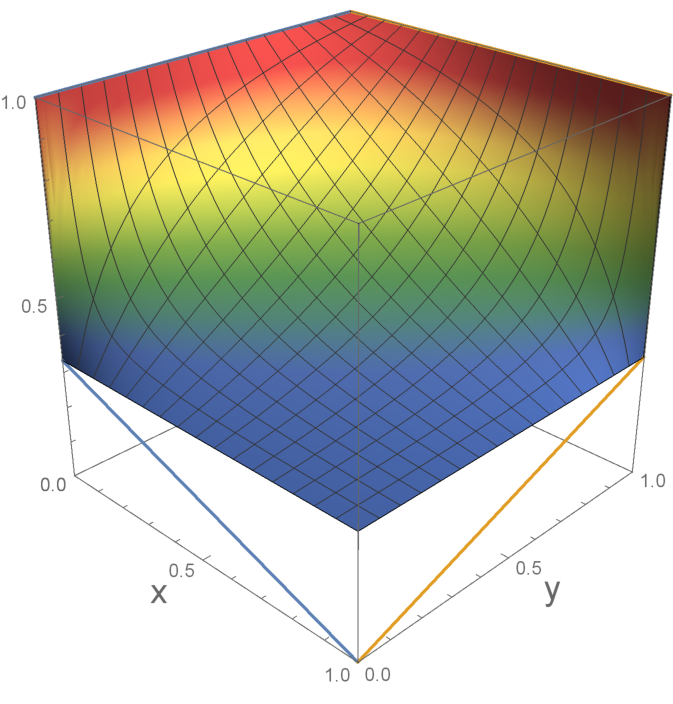
\includegraphics[width=.6\linewidth]{Ex1.pdf}
				\caption{$I_1$}
				\label{exfig:strict:TPowerInv:subfig1}
			\end{subfigure}%
			\begin{subfigure}{.5\textwidth}
				\centering
				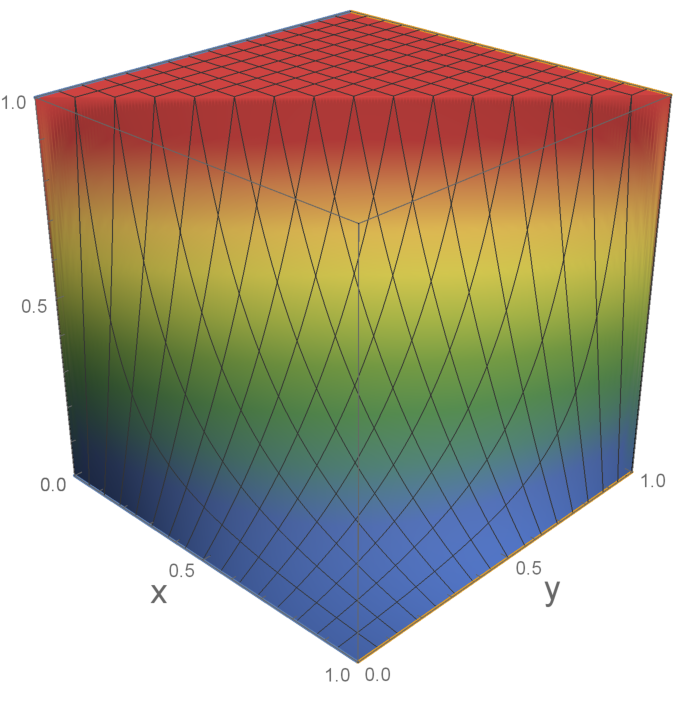
\includegraphics[width=.6\linewidth]{Ex2.pdf}
				\caption{$I_2$}
				\label{exfig:strict:TPowerInv:subfig2}
			\end{subfigure}
			\caption[Plot of two examples of strict $T$-power invariant implications.]{Plots of fuzzy implication functions given in Example \ref{ex:strict:TPowerInv}.}
			\label{exfig:strict:TPowerInv}
		\end{figure}
	\end{enumerate}
\end{example}

\subsection{Nilpotent $T$-power invariant implications}\label{subsection:nilpotentTpowerimplications}

The authors in \cite{Massanet2019B} proposed the following characterization of all binary mappings satisfying the $T$-power invariance with respect to a nilpotent Archimedean t-norm $T$ in terms of an additive generator $t$ such that $t(0)>1$.

\begin{proposition}[{\bf \cite[Proposition~11]{Massanet2019B}}]\label{prop:nilpot:mistake}
	Let $T$ be a nilpotent t-norm and $t$ an additive generator of $T$ with $t(0)>1$. Then a mapping $I:[0,1]^2 \to [0,1]$ is invariant with respect to $T$-powers if and only if there exists a mapping $\varphi:(0,+\infty) \to [0,1]$ such that $I$ is given by
	$$I(x,y)=\varphi \left(\frac{t(x)}{t(y)}\right), \quad \text{for all } x,y \in (0,1) \text{ such that } \frac{t(x)}{t(y)}<t(0).$$
\end{proposition}

However, the next example shows that the result is not entirely correct since it provides necessary but not sufficient conditions.

\begin{example}\label{example:nilpot:counterexample}
	Let us consider the Łukasiewicz t-norm \TLK, the additive generator $t(x)=2(1-x)$ for all $ x \in [0,1]$ with $t(0)=2$ and the following binary function
	\begin{equation*}
		I(x,y) =\left\{ \begin{array}{ll}
			\frac{1}{2} \cdot \frac{1-x}{1-y} & \text{if } \frac{1-x}{1-y}<2,\\
			x &   \text{otherwise}.
		\end{array}
		\right.
	\end{equation*}
	If we define $\varphi:(0,+\infty) \to (0,1)$ with $\varphi(w)=\frac{w}{2}$ for all $w \in (0,+\infty)$ we have $I(x,y)= \frac{1}{2} \cdot \frac{1-x}{1-y} =\varphi \left( \frac{t(x)}{t(y)} \right)$ for all $x,y \in [0,1]$ such that $\frac{1-x}{1-y}<2$. Then, the function $I$ fulfills the conditions in Proposition \ref{prop:nilpot:mistake}. However, let us show that $I$ is not invariant with respect to $T$-powers. Consider $x=r=\frac{1}{2}$ and $y = \frac{7}{8}$, then
	$$ x_T^{(r)} = t^{-1}(\min\{t(0),rt(x)\})= t^{-1}(1-x) = \frac{1}{2}+ \frac{x}{2}=\frac{1}{2} + \frac{1}{4}=\frac{3}{4}, \quad y_T^{(r)} = \frac{1}{2} +\frac{y}{2}=\frac{1}{2} + \frac{7}{16} = \frac{15}{16}.$$ 
	In this case,
	$$I(x,y)=I\left(\frac{1}{2},\frac{7}{8}\right) = \frac{1}{2} \not = \frac{3}{4} = I\left(\frac{3}{4}, \frac{15}{16} \right) = I\left(x_T^{(r)},y_T^{(r)}\right).$$
\end{example}

Therefore, differently from the case of strict T-power invariant implications, before presenting the family of nilpotent $T$-power invariant implications we need to study which binary functions are invariant with respect to the positive powers of a nilpotent t-norm, fixing the previous result. In the next result, we present a new characterization of such functions.

\begin{theorem}\label{thm:nilpot:invimp}
	Let $T$ be a nilpotent t-norm and $t$ an additive generator of $T$. Then a mapping $I:[0,1]^2 \to [0,1]$ is invariant with respect to $T$-powers if and only if there exists a mapping $\varphi:(0,+\infty) \to [0,1]$ such that $I$ is given by
	\begin{equation}\label{eq:nilpot:invimpl}
		I(x,y)=\varphi \left(\frac{t(x)}{t(y)}\right), \quad \text{for all } x,y \in (0,1).
	\end{equation}
\end{theorem}
\begin{proof} Let $T$ be a nilpotent t-norm, $t$ an additive generator of $T$ and $I:[0,1]^2 \to [0,1]$ a binary function.
	\begin{itemize}
		\item[$(\Rightarrow)$] Consider the following partition $\displaystyle (0,+\infty)=(0,2) \cup  \bigcup_{n \in \NN}[2^n,2^{n+1})$. Now, let us define the following family of functions
		$$
		\begin{array}{rcl}
			\varphi_0:\left(0,2\right)&\longrightarrow&[0,1]\\
			z&\longmapsto& I\left(t^{-1}\left(\frac{t(0)}{2}z\right),t^{-1}\left(\frac{t(0)}{2}\right)\right),
		\end{array}
		$$
		$$
		\begin{array}{rcl}
			\varphi_n:\left[2^n,2^{n+1}\right)&\longrightarrow&[0,1]\\
			z&\longmapsto& I\left(t^{-1}\left(\frac{t(0)}{2^{n+1}}z\right),t^{-1}\left(\frac{t(0)}{2^{n+1}}\right)\right)
		\end{array},
		\quad
		\text{for all } n \in \NN.
		$$
		These functions are well defined because $\frac{t(0)}{2^{n+1}} \in (0,t(0))$ and
		$$\frac{t(0)}{2^{n+1}}z \in \left[\frac{t(0)}{2^{n+1}} \cdot 2^n ,\frac{t(0)}{2^{n+1}} \cdot 2^{n+1}\right) = \left[\frac{t(0)}{2},t(0)\right) \subseteq (0,t(0)),$$
		for all $n \in \NN$ and $z \in [2^n,2^{n+1})$. Consider the function $\varphi$ defined as follows
		$$
		\begin{array}{rcll	}
			\varphi:(0,+\infty)&\longrightarrow&[0,1]\\
			z&\longmapsto& \varphi_n(z) &\text{if } z \in [2^n,2^{n+1})\\
			z&\longmapsto& \varphi_0(z) &\text{if } z \in (0,2)
		\end{array}.
		$$
		Let us see that $I(x,y)= \varphi \left(\frac{t(x)}{t(y)}\right)$ for all $x,y \in (0,1)$. Since $I$ is $T$-power invariant, then
		$$I(x,y)= I(t^{-1}(rt(x)),t^{-1}(rt(y))),$$
		for all $x,y \in (0,1)$ and $r < \min \left\lbrace\frac{t(0)}{t(x)},\frac{t(0)}{t(y)}\right\rbrace$. Let $x_0,y_0 \in (0,1)$, we distinguish between two cases:
		\begin{itemize}
			\item If $\frac{t(x_0)}{t(y_0)} \in \left[2^n,2^{n+1}\right)$ for some $n \in \NN$, considering $r_0= \frac{t(0)}{2^{n+1}t(y_0)}$ we have that
			$$\frac{t(x_0)}{t(y_0)}< 2^{n+1} \Rightarrow \frac{t(0)}{t(x_0)} > \frac{t(0)}{2^{n+1}t(y_0)} =r_0 \Rightarrow r_0 < \min \left\lbrace\frac{t(0)}{t(x_0)},\frac{t(0)}{t(y_0)}\right\rbrace.$$
			Therefore, 
			\begin{eqnarray*}
				I(x_0,y_0)&=&I(t^{-1}(r_0t(x_0)),t^{-1}(r_0t(y_0)))=I\left(t^{-1}\left(\frac{t(0)}{2^{n+1}}\frac{t(x_0)}{t(y_0)}\right),t^{-1}\left(\frac{t(0)}{2^{n+1}}\right)\right) \\
				&=&\varphi_n\left(\frac{t(x_0)}{t(y_0)}\right) = \varphi \left(\frac{t(x_0)}{t(y_0)}\right).
			\end{eqnarray*}
			\item If $\frac{t(x_0)}{t(y_0)} \in \left(0,2\right)$ then considering $r_0= \frac{t(0)}{2t(y_0)}$ and with an analogous argument to the previous point we obtain that $I(x_0,y_0)=\varphi_0\left(\frac{t(x_0)}{t(y_0)}\right)=\varphi\left(\frac{t(x_0)}{t(y_0)}\right)$.
		\end{itemize}
		\item[$(\Leftarrow)$] Consider that there exists a function $\varphi:(0,+\infty) \to [0,1]$ such that $I$ is given by Equation (\ref{eq:nilpot:invimpl}). We have to prove that $I(x_T^{(r)},y_T^{(r)})=I(x,y)$ for all $r>0$ and $x,y \in [0,1]$ such that $x_T^{(r)},y_T^{(r)} \not \in \{0,1\}$. Since $T$ is a nilpotent t-norm we have that whenever $x_T^{(r)} \not = 0$ then $x_T^{(r)}=t^{-1}(rt(x))$. In this case, we have that
		$$I(x_T^{(r)},y_T^{(r)})=\varphi \left(\frac{t(x_T^{(r)})}{t(y_T^{(r)})}\right)
		=\varphi \left(\frac{rt(x)}{rt(y)}\right) =\varphi \left(\frac{t(x)}{t(y)}\right)=I(x,y).$$
	\end{itemize}
\end{proof}

This result reveals that the structure of functions which are $T$-power invariant is the same in the strict and nilpotent cases (see Proposition \ref{prop:strict:charactbintpowerinv}). Moreover, differently from Proposition \ref{prop:nilpot:mistake}, Equation (\ref{eq:nilpot:invimpl}) is also valid for additive generators with $t(0) \leq 1$. In consequence of this dependence, in \cite{Massanet2019B} the authors only studied fuzzy implication functions which are invariant with respect to the positive powers of a nilpotent t-norm and also satisfy \IP. In our case, thanks to the previous result we can easily characterize all the fuzzy implication functions that are invariant with respect to the positive powers of a nilpotent t-norm without further restrictions.

It is well known that the additive generators of nilpotent t-norms differ from those from strict t-norms in the fact that their image is $[0,t(0)]$ with $t(0)<+\infty$. We will see along the chapter that this fact makes a huge difference between the strict and nilpotent cases. The next trivial lemma will be useful throughout the chapter to the manipulation of Equation  (\ref{eq:nilpot:invimpl}) in the nilpotent case.
\begin{lemma}\label{lem:nilpot:values} 
	Let $w_1,w_2 \in (0,+\infty)$ with $w_1 \leq w_2$ and $t$ an additive generator of a nilpotent t-norm. Then there exist $y^*,x_1,x_2 \in (0,1)$ with $x_1 \geq x_2$ such that $w_1=\frac{t(x_1)}{t(y^*)}$ and $w_2=\frac{t(x_2)}{t(y^*)}$.
\end{lemma}
\begin{proof}
	Since $t$ is a continuous, strictly decreasing function then $\left\lbrace \frac{t(0)}{t(y)} \bigm| y \in (0,1)\right\rbrace = (1,+\infty)$ and there exists a $y^* \in (0,1)$ such that $w_1,w_2 \in \left(0,\frac{t(0)}{t(y^*)}\right)$. On the other hand, we have that $\left\lbrace \frac{t(x)}{t(y^*)} \bigm| x \in (0,1)\right\rbrace = \left(0,\frac{t(0)}{t(y^*)}\right)$ and then there exist $x_1,x_2 \in (0,1)$ such that $w_1=\frac{t(x_1)}{t(y^*)}$ and $w_2=\frac{t(x_2)}{t(y^*)}$. Since $t$ is a strictly decreasing function and $w_1 \leq w_2$ we know that $x_1 \geq x_2$.
\end{proof}

The next result restricts Theorem \ref{thm:nilpot:invimp} to fuzzy implication functions.

\begin{proposition}\label{prop:nilpot:TPowerInv}
	Let $T$ be a nilpotent t-norm and $t$ an additive generator of $T$. A mapping $I:[0,1]^2 \to [0,1]$ is a fuzzy implication function invariant with respect to $T$-powers if and only if $f(x)=I(x,0)$ for all $x \in (0,1)$ is decreasing, $g(y)=I(1,y)$ for all $y \in (0,1)$ is increasing and there exists an increasing function $\varphi:[0,+\infty] \to [0,1]$ such that $\varphi(0)=0$, $\varphi(+\infty)=1$, 
	\begin{equation}\label{eq:prop:nilpot:TPowerInv:MonotonicityCond}
		f(x) \leq \inf_{y \in (0,1)} \varphi \left(\frac{t(x)}{t(y)}\right), \quad \text{for all } x \in (0,1), \quad
		g(y) \leq \inf_{x \in (0,1)} \varphi \left(\frac{t(x)}{t(y)}\right), \quad \text{for all } y \in (0,1),
	\end{equation}
	and $I$ is given by
	\begin{equation}\label{eq:prop:nilpot:TPowerInv:Expression}
		I(x,y) =\left\{ \begin{array}{ll}
			1 & \text{if } x=0 \text{ and } y \in [0,1),\\
			f(x) &   \text{if }   x \in (0,1) \text{ and } y=0, \\
			g(y) &  \text{if }  x = 1 \text{ and } y\in (0,1), \\
			\varphi \left(\frac{t(x)}{t(y)}\right) &  \text{otherwise},
		\end{array}
		\right.
	\end{equation}
	with the understanding $\frac{0}{0} = +\infty$.
\end{proposition}
\begin{proof}
	Let $I$ be a fuzzy implication function which is invariant with respect to $T$-powers. By Theorem \ref{thm:nilpot:invimp} 
	we know that there exists a function $\varphi:(0,+\infty) \to [0,1]$ such that
	$$I(x,y)=\varphi \left(\frac{t(x)}{t(y)}\right), \quad \text{for all }x,y \in (0,1).$$
	We extend this function to $[0,+\infty]$ by defining $\varphi(0)=0$ and $\varphi(+\infty)=1$. Let us define $f(x)=I(x,0)$ for all $x \in (0,1)$ and $g(y)=I(1,y)$ for all $y \in (0,1)$. It is clear that by \Ione, $f$ is decreasing and by \Itwo $g$ is increasing. Now, we prove that $\varphi$ is increasing. Consider $w_1,w_2 \in (0,+\infty)$ with $w_1 \leq w_2$. By Lemma \ref{lem:nilpot:values} we know that there exist $x_1,x_2,y^* \in (0,1)$ with $x_1 \geq x_2$ such that $w_1=\frac{t(x_1)}{t(y^*)}$ and $w_2=\frac{t(x_2)}{t(y^*)}$. Now, by \Ione we have
	$$\varphi(w_1) = \varphi \left(\frac{t(x_1)}{t(y^*)}\right) = I(x_1,y^*) \leq I(x_2,y^*) = \varphi \left(\frac{t(x_2)}{t(y^*)}\right) = \varphi(w_2),$$
	and $\varphi$ is increasing. Then, $I$ has the structure in Equation (\ref{eq:prop:nilpot:TPowerInv:Expression}). Consider $\tilde{x},\tilde{y} \in (0,1)$, then by \Ione and \Itwo we have
	$$f(\tilde{x}) = I(\tilde{x},0) \leq I(\tilde{x},y) = \varphi \left( \frac{t(\tilde{x})}{t(y)} \right), \quad \text{for all } y \in (0,1),$$
	$$g(\tilde{y})=I(1,\tilde{y}) \leq I(x,\tilde{y})= \varphi\left(\frac{t(x)}{t(\tilde{y})}\right), \quad \text{for all } x \in (0,1).$$
	Then, $I$ fulfills Condition (\ref{eq:prop:nilpot:TPowerInv:MonotonicityCond}). For the reverse implication, assume that there exist a decreasing function $f:(0,1) \to [0,1]$ and increasing functions $\varphi:[0,+\infty] \to [0,1]$, $g:(0,1) \to [0,1]$ such that $\varphi(0)=0$, $\varphi(+\infty)=1$ and fulfill Condition (\ref{eq:prop:nilpot:TPowerInv:MonotonicityCond}). Let us see that $I$ given by Equation (\ref{eq:prop:nilpot:TPowerInv:Expression}) is a fuzzy implication function.
	\begin{itemize}
		\item Let $x_1,x_2,y \in [0,1]$ with $x_1 < x_2$, then we distinguish between three cases:
		\begin{itemize}
			\item If $y=0$ then since $f$ is decreasing we have $I(x,0)=f(x_1) \geq f(x_2)=I(x_2,0).$
			\item If $y=1$ then $I(x_1,1)=I(x_2,1)=1$.
			\item  If $ y \in (0,1)$ we have
			\begin{itemize}
				\item If $x_1=0$ then $I(x_1,y)=I(0,y)=1 \geq I(x_2,y).$
				\item If $x_1,x_2 \in (0,1)$ then $I(x_1,y)=\varphi \left(\frac{t(x_1)}{t(y)}\right) \geq \varphi \left(\frac{t(x_2)}{t(y)}\right) = I(x_2,y).$
				\item If $x_1 \in (0,1)$ and $x_2=1$ then $I(x_1,y)=\varphi \left(\frac{t(x_1)}{t(y)}\right) \geq g(y)=I(1,y)=I(x_2,y).$
			\end{itemize}
		\end{itemize} 
		Therefore, $I$ fulfills \Ione.
		\item Analogously to the previous point we verify that $I$ fulfills \Itwo.
		\item Since
		$$ I(1,1)= \PHI{1}{1} = \varphi\left(\frac{0}{0}\right)= \varphi(+\infty)=1, \quad I(0,0)=1,$$
		$$I(1,0)=\PHI{1}{0}=\varphi(0)=0,$$
		we have that $I$ satisfies \Ithree. \qedhere
	\end{itemize}
\end{proof}

Now, in view of the last result, we can define the family of fuzzy implication functions characterized by the fact that they are $T$-power invariant with respect to a certain nilpotent t-norm.

\begin{definition}\label{def:nilpot:TPowerInv}
	Let $T$ be a nilpotent t-norm and $t$ an additive generator of $T$. Let $f:(0,1) \to [0,1]$ be a decreasing function and $\varphi:[0,+\infty] \to [0,1]$, $g: (0,1) \to [0,1]$ increasing functions such that $\varphi(0)=0$, $\varphi(+\infty)=1$ and
	\begin{equation}\label{eq:def:nilpot:TPowerInv:MonotonicityCond}
		f(x) \leq \inf_{y \in (0,1)} \varphi \left(\frac{t(x)}{t(y)}\right), \quad \text{for all } x \in (0,1), \quad
		g(y) \leq \inf_{x \in (0,1)} \varphi \left(\frac{t(x)}{t(y)}\right), \quad \text{for all } y \in (0,1).
	\end{equation}
	The function $\IT:[0,1]^2 \to [0,1]$ defined  by
	\begin{equation}\label{eq:nilpot:TPowerInv:Expression}
		I^T_{\varphi,f,g}(x,y) =\left\{ \begin{array}{ll}
			1 & \text{if } x=0 \text{ and } y \in [0,1),\\
			f(x) &   \text{if }   x \in (0,1) \text{ and } y=0, \\
			g(y) &  \text{if }  x = 1 \text{ and } y\in (0,1), \\
			\varphi \left(\frac{t(x)}{t(y)}\right) &  \text{otherwise},
		\end{array}
		\right.
	\end{equation}
	with the understanding $\frac{0}{0} = + \infty$, is called a \emph{nilpotent $T$-power invariant implication}.
\end{definition}

In view of Definitions \ref{def:strict:TPowerInv} and \ref{def:nilpot:TPowerInv}, we can notice that the structure of strict and nilpotent $T$-power invariant implications is very similar (see Figure \ref{fig:TPowerInv}). However, despite this fact we show further in this chapter that both families behave differently.
% Figure 1 %
\begin{figure}[H]
		\centering
		\begin{tikzpicture}[xscale=3, yscale=3]
				\draw (0,0) rectangle (1,1);
				\node [above right] at (1,1) {1} ;
				\node [below right] at (1,0) {0};
				\node [below left] at (0,0) {1};
				\node [above left] at (0,1) {1};
				\node [above] at (0.5,1) {1};
				\node [below] at (0.5,0) {$f(x)$};
				\node [left] at (0,0.5) {1};
				\node [right] at (1,0.5) {$g(y)$};
				\node at (0.5,0.5) {\large $\varphi \left( \frac{t(x)}{t(y)} \right)$};
			\end{tikzpicture}
		\caption{Schema of the structure of the family of strict and nilpotent $T$-power invariant implications.}
		\label{fig:TPowerInv}
\end{figure}

A first difference between Definition \ref{def:nilpot:TPowerInv} and the analogous definition for strict t-norms (see Definition \ref{def:strict:TPowerInv}) is that Condition (\ref{eq:def:nilpot:TPowerInv:MonotonicityCond}) is more complex than Condition (\ref{eq:strict:TPowerInv:MonotonicityCond}). In this case, if $I$ is a fuzzy implication function invariant with respect to $T$-powers where $T$ is a nilpotent t-norm, then  the function $\varphi$ is not necessarily bounded below by any possible value of $f$. For instance, the following example corresponds to a nilpotent $T$-power invariant implication with $\Ima \varphi = [0,1]$ and $f(x)=1-x$ for all $x \in (0,1)$.

\begin{example}\label{ex:nilpot:TPowerInv}
	Let us consider the Łukasiewicz t-norm \TLK, the additive generator $t(x)=1-x$ for all $x \in [0,1]$, $\varphi(w)=w$ for all $w \in [0,1]$, $\varphi(w)=1$ for all $ w \in (1,+\infty]$, $f(x)=1-x$ for all $x \in (0,1)$ and $g(y)=0$ for all $ y \in (0,1)$. We have that $\varphi$, $f$ and $g$ fulfill Condition (\ref{eq:def:nilpot:TPowerInv:MonotonicityCond}) and then the function given by
	$$
	I(x,y) =\left\{ \begin{array}{ll}
		1-x &   \text{if }   x \in (0,1) \text{ and } y=0, \\
		0 &  \text{if }  x = 1 \text{ and } y\in [0,1), \\
		\frac{1-x}{1-y} &  \text{if } x,y \in (0,1) \text{ and } x \geq y, \\
		1 & \text{otherwise,}
	\end{array}
	\right.
	$$
	is a fuzzy implication function which is invariant with respect to the positive powers of \TLK. The plot of this fuzzy implication function is displayed in Figure \ref{exfig:nilpot:TPowerInv}.
	\begin{figure}[!htp]
		\centering
		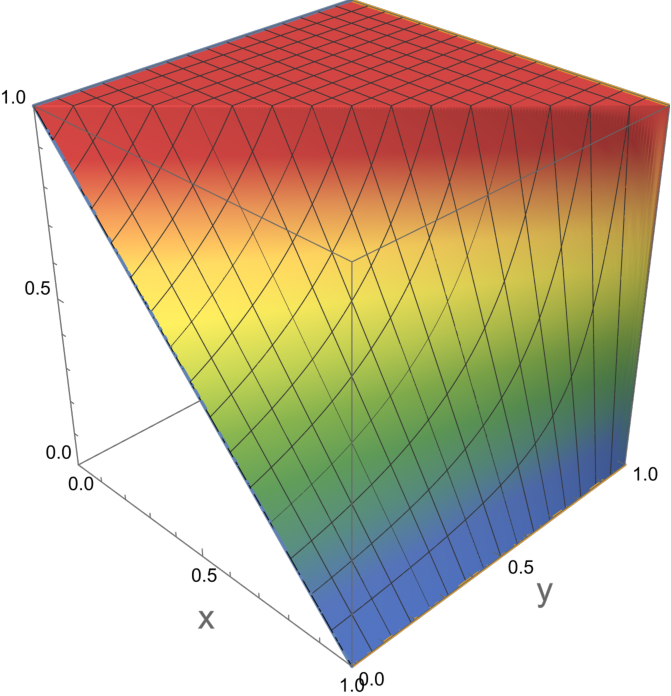
\includegraphics[scale=0.5]{Example0.pdf}
		\caption[Plot of an example of a nilpotent $T$-power invariant implication.]{Plot of the fuzzy implication function constructed in Example \ref{ex:nilpot:TPowerInv}.}\label{exfig:nilpot:TPowerInv}
	\end{figure}
\end{example}

However, we can simplify Condition (\ref{eq:def:nilpot:TPowerInv:MonotonicityCond}) in terms of the following necessary condition.
\begin{lemma}\label{lem:nilpot:monotonicity_condition:necessicity}
	Let \IT be a nilpotent $T$-power invariant implication, then
	\begin{equation*}
		\sup_{x \in (0,1)} f(x) \leq \inf_{w \in (1,+\infty)} \varphi(w), \quad \sup_{y \in (0,1)} g(y) \leq \inf_{w \in (0,+\infty)} \varphi(w).
	\end{equation*}
\end{lemma}
\begin{proof}
	Let us consider $\tilde{x} \in (0,1)$ and $w_0 \in (1,+\infty)$,  since $t$ is a continuous, strictly decreasing function then $\left\lbrace \frac{t(\tilde{x})}{t(y)} \bigm| y \in (0,1) \right\rbrace = \left(\frac{t(\tilde{x})}{t(0)},+\infty\right)$ with $\frac{t(\tilde{x})}{t(0)}<1$ and $ w_0 \in (1,+\infty)\subseteq \left (\frac{t(\tilde{x})}{t(0)},+\infty\right )$. Thus, there exists a $y_0 \in (0,1)$ with $w_0 = \frac{t(\tilde{x})}{t(y_0)}$ and by \Itwo we have
	$$f(\tilde{x}) = I(\tilde{x},0) \leq I(\tilde{x},y_0) = \PHI{\tilde{x}}{y_0}=\varphi(w_0).$$
	On the other hand, we consider $\tilde{y} \in (0,1)$ and $w_1 \in (0,+\infty)$ and we prove that $g(\tilde{y}) \leq \varphi(w_1)$. Since $\varphi$ is increasing it is enough to consider $w_1 \in (0,1)$. We know that $\left\lbrace \frac{t(x)}{t(\tilde{y})} \bigm| x \in (0,1)\right\rbrace = \left(0,\frac{t(0)}{t(\tilde{y})}\right)$ with $\frac{t(0)}{t(\tilde{y})}>1$ and then $w_1 \in (0,1)\subseteq \left(0,\frac{t(0)}{t(\tilde{y})}\right)$. Thus, there exists an $x_1 \in (0,1)$ with $\frac{t(x_1)}{t(\tilde{y})}=w_1$ and  by \Ione we have
	$$g(\tilde{y})=I(1,\tilde{y}) \leq I(x_1,\tilde{y})=\varphi\left(\frac{t(x_1)}{t(\tilde{y})}\right) =\varphi(w_1).$$
\end{proof}

The following example shows that Lemma \ref{lem:nilpot:monotonicity_condition:necessicity} is not sufficient.

\begin{example}
	Let us consider the Łukasiewicz t-norm \TLK, the additive generator $t(x)=1-x$ for all $x \in [0,1]$, $\varphi(w)=w$ for all $w \in [0,1]$, $\varphi(w)=1$ for all $w \in (1,+\infty]$, $f(x)=1-x^2$ for all $x \in (0,1)$ and $g(y)=0$ for all $ y \in (0,1)$. Let $I$ be the function given by Equation (\ref{eq:nilpot:TPowerInv:Expression}). For $x=\frac{1}{2}$ and $y=\frac{1}{4}$ we have
	$$f\left( \frac{1}{2} \right) = \frac{3}{4} > \frac{2}{3} = I\left(\frac{1}{2},\frac{1}{4}\right),$$
	and since $I$ does not fulfill Condition (\ref{eq:def:nilpot:TPowerInv:MonotonicityCond}), $I$ is not a nilpotent \TLK-power invariant implication. However, we have
	$$\sup_{x \in (0,1)} f(x) = 1= \inf_{w \in (1,+\infty)} \varphi(w), \quad \sup_{y \in (0,1)} g(y)=0 = \inf_{w \in (0,+\infty)} \varphi(w).$$
\end{example}

\begin{remark}
	Let $T$ be a nilpotent (resp. strict) t-norm, when we consider a nilpotent (resp. strict) $T$-power invariant implication $\IT$ we are always assuming that there exist functions $\varphi$, $g$ and $f$ that fulfill all the conditions in Definition \ref{def:nilpot:TPowerInv} (resp. Definition \ref{def:strict:TPowerInv}) even when not explicitly mentioned. For instance, if we say ``Let us consider \IT a nilpotent $T$-power invariant implication with $f(x)\geq 0.5$ for all $x \in (0,1)$'', then $f:(0,1) \to [0,1]$ must be a decreasing function with $0.5 \leq f(x) \leq \inf_{y \in (0,1)} \varphi \left(\frac{t(x)}{t(y)}\right)$ for all $x \in (0,1)$, whenever this is allowed by the structure of $\varphi$.
\end{remark}

\section{Additional properties of strict and nilpotent $T$-power invariant implications}\label{section:additional_propertiesTpower}

In this section, we study other additional properties aside from the invariance with respect to $T$-powers that can be satisfied by the family of strict and nilpotent $T$-power implications. The additional properties we have decided to study are: continuity, natural negation, trivial 1-region, \CB, \NP, \IP, \OP, \EP, \LI, \IB and \TC. We have chosen these properties because they are among the most popular additional properties of fuzzy implication functions. Also, the study of these properties (specially \NP and \EP) is essential for the determination of the intersection between these families and others (see Section \ref{section:intersectionsTpower}). Due to several differences, we perform a separate study for strict and nilpotent $T$-power implications.

\subsection{Additional properties of strict $T$-power invariant implications}\label{subsection:additional_propertiesStrictTpower}

First of all, we establish under which conditions on $\varphi$, $f$ and $g$, the corresponding \STP is continuous on a point of its domain.
% Continuity %
\begin{proposition} \label{prop:strict:continuity} Let $\IT$ be a \STP. The following statements hold:
	\begin{enumerate}[label=(\roman*)]
		\item If $\varphi$ is continuous on $w=0$, then $f(x)=g(y)=0$ for all $x,y \in (0,1)$.
		\item If $\displaystyle \lim_{x \to 0^+} f(x)=1$ or $\displaystyle \lim_{y \to 1^-}g(y)=1$, then $\varphi(w)=1$ for all $w \in (0,+\infty)$.
		\item $\IT$ is continuous on $(x,0)$ for $x \in (0,1)$ if and only if $\displaystyle f(x)= \lim_{w \to 0^+} \varphi(w)$.
		\item $\IT$ is continuous on $(1,y)$ for $y \in (0,1)$ if and only if $\displaystyle g(y)= \lim_{w \to 0^+} \varphi(w)$.
		\item $\IT$ is continuous on $(x,1)$ and $(0,x)$ for all $x \in [0,1]$ if and only if $\displaystyle \lim_{w \to +\infty} \varphi(w)=1$.
		\item $\IT$ is continuous on $(x_0,y_0)$ with $x_0,y_0 \in (0,1)$ if and only if $\varphi$ is continuous on $\frac{t(x_0)}{t(y_0)}$. In this case, $\IT$ is also continuous on the following points
		$$\left(x,t^{-1}\left(\frac{t(x)t(y_0)}{t(x_0)}\right)\right), \quad \text{for all } x \in (0,1).$$
	\end{enumerate}
\end{proposition}
\begin{proof}Statements (i) and (ii) are direct consequences of Condition (\ref{eq:strict:TPowerInv:MonotonicityCond}).
	\begin{enumerate}[label=(\roman*)]
		\item[(iii)] $\IT$ is continuous on $(x_0,0)$ for $x_0 \in (0,1)$ if and only if
		$$f(x_0)=\IT(x_0,0)=\lim_{(x,y) \to (x_0,0)}\IT(x,y) = \lim_{(x,y) \to (x_0,0)} \varphi\left(\frac{t(x)}{t(y)}\right).$$
		Now, by considering the change of variables $w=\frac{t(x)}{t(y)}$ we obtain
		$$\lim_{(x,y) \to (x_0,0)} \varphi\left(\frac{t(x)}{t(y)}\right)=\lim_{w \to 0^+} \varphi(w).$$
		\item[(iv)] The proof is analogous to the Case (iii).
		\item[(v)] $\IT$ is continuous on $(x_0,1)$ for $x_0 \in[0,1]$ if and only if
		$$1=I(x_0,1)=\lim_{(x,y) \to (x_0,1)}I(x,y)=\lim_{(x,y) \to (x_0,1)}\varphi\left(\frac{t(x)}{t(y)}\right)=\lim_{w \to +\infty}\varphi(w).$$ 
		On the other hand, $\IT$ is continuous $(0,x_0)$ for $x_0 \in[0,1]$ if and only if
		$$1=\IT(0,x_0)=\lim_{(x,y) \to (0,x_0)}I(x,y)=\lim_{(x,y) \to (0,x_0)}\varphi\left(\frac{t(x)}{t(y)}\right)=\lim_{w \to +\infty}\varphi(w).$$
		\item[(vi)] $\IT$ is continuous on $(x_0,y_0)$ for $x_0,y_0 \in (0,1)$ if and only if
		$$I(x_0,y_0)=\lim_{(x,y) \to (x_0,y_0)} I(x,y)=\lim_{(x,y) \to (x_0,y_0)} \varphi \left(\frac{t(x)}{t(y)}\right) = \lim_{w \to \frac{t(x_0)}{t(y_0)}}\varphi(w).$$
		Now, since the points $(a_x,b_x)=\left(x,t^{-1}\left(\frac{t(x)t(y_0)}{t(x_0)}\right)\right)$ are such that $\frac{t(a_x)}{t(b_x)}=\frac{t(x_0)}{t(y_0)}$ for all $x \in (0,1)$, we have that $\IT$ is also continuous on $(a_x,b_x)$. \qedhere
	\end{enumerate}
\end{proof}
Notice that the previous proposition implies that imposing continuity in certain points of a \STP leads to consider that $\varphi$, $f$ or $g$ are constant. This is due to Condition (\ref{eq:strict:TPowerInv:MonotonicityCond}), which imposes that the function $\varphi$ is bounded below by any possible value of $f$ and $g$ (see Example \ref{ex:strict:TPowerInv}). Then, although the structure of strict $T$-power implications may seem flexible since it depends on three unknown functions, as a matter of fact, Condition (\ref{eq:strict:TPowerInv:MonotonicityCond}) severely restricts the choices of functions $\varphi$, $f$ and $g$ for which \IT is a fuzzy implication function. Moreover, from (ii)-Proposition \ref{prop:strict:continuity} it is easy to see that \IT is never a continuous function.

\begin{corollary}\label{cor:strict:discontinuous} Let \IT be a \STP. Then at least one of the following conditions holds:
	\begin{enumerate}[label=(\roman*)]
		\item $\IT$ is discontinuous on (1,0).
		\item $\IT$ is discontinuous on (0,0) or (1,1).
	\end{enumerate}
\end{corollary}
\begin{proof} Let us consider \IT a \STP. If \IT is continuous on $(0,0)$ then
	$$ 1=\IT(0,0)= \lim_{x \to 0^+} \IT(x,0) = \lim_{x \to 0^+} f(x), $$
	and by {(ii)-Proposition \ref{prop:strict:continuity}} we get that $\varphi(w)=1$ for all $w \in (0,+\infty)$. Therefore, $\IT(x,y)=1$ for all $(x,y) \in (0,1)^2$. Since $I^T_{\varphi,f,g}(1,0)=0$, $I^T_{\varphi,f,g}$ is discontinuous on $(1,0)$.
	On the other hand, if \IT is continuous on $(1,1)$ then
	$$1=\IT(1,1)= \lim_{y \to 1^-} \IT(1,y) = \lim_{y \to 1^-} g(y), $$
	and again by {(ii)-Proposition \ref{prop:strict:continuity}} we have that $\IT(x,y)=1$ for all $(x,y) \in (0,1)^2$ and then \IT is not continuous on $(1,0)$.
\end{proof}
In terms of the natural negation of a \STP, it is straightforward to see that it is completely determined by the function $f$. Therefore, we can always find strict $T$-power implications  whose natural negation is a certain fuzzy negation $N$. However, again by {(ii)-Proposition \ref{prop:strict:continuity}} we remark that if the natural negation of $\IT$ is continuous on $x=0$ necessarily $\IT$ is constant to 1 in $(0,1)^2$.

% Natural Negation %
\begin{corollary}\label{cor:strict:natural_negation} Let \IT be a \STP. The natural negation of $\IT$ is given by
	$$ N_{\IT}(x)=\left\{ \begin{array}{ll}
		1 &  \text{if }  x=0, \\
		f(x) & \text{if }  x \in(0,1),\\
		0 &  \text{if }x=1.
	\end{array}
	\right.
	$$
	Moreover, if $N_{\IT}$ is continuous on $x=0$ (in particular, when $N_{\IT}$ is a strong or strict negation), then $\IT(x,y)=1$ for all $x,y \in (0,1)^2$.
\end{corollary}
\begin{proof} 
	Let us consider \IT a \STP, then by definition we have that
	$$
	N_{\IT}(x)=\IT(x,0)= \left\{ \begin{array}{ll}
		1 &  \text{if }  x=0, \\
		f(x) & \text{if }  x \in(0,1),\\
		0 &  \text{if }x=1.
	\end{array}
	\right.
	$$
	Now, if it is continuous on $x=0$ then $\displaystyle 1=\lim_{x \to 0^+} N_{\IT}(x) = \lim_{x \to 0^+} f(x)$ and by {(ii)-Proposition \ref{prop:strict:continuity}} we have that $\varphi(w)=1$ for all $w \in (0,+\infty)$. Therefore, $\IT(x,y)=1$ for all $x,y \in (0,1)$.
\end{proof}
% 1-region %
With respect to the 1 and 0-region of a \STP, it is straightforward to see that the region where \IT equals 0 or 1 directly depends on the intervals where the functions $\varphi$, $f$ and $g$ equal 0 or 1, respectively (see Examples \ref{ex:strict:TPowerInv} and \ref{example:strict:(IB)}). However, the next proposition characterizes when $I$ has a trivial 1-region.

\begin{proposition}\label{prop:strict:1-region}
	 Let \IT be a \STP. Then $(I(x,y)=1 \Leftrightarrow x=0 \text{ or } y=1)$ if and only if $f(x),g(y)<1$ for all $x,y \in (0,1)$ and $\varphi(w)<1$ for all $w \in (0,+\infty)$.
\end{proposition} 
\begin{proof} Straightforward from Definition \ref{def:strict:TPowerInv}.
\end{proof}

% Consequent boundary %
The following result studies when strict $T$-power invariant implications satisfy the consequent boundary. In this case, we see that $\IT$ needs to be constant to 1 in $(0,1)^2$ and $g(y) \geq y$ for all $y \in (0,1)$.
\begin{proposition}\label{prop:strict:(CB)} Let $\IT$ be a strict $T$-power invariant implication. Then $\IT$ satisfies \CB if and only if $g(y) \geq y$ for all $y \in (0,1)$. Moreover, in this case \IT is given by
	\begin{equation}\label{eq:(CB)}
		\IT(x,y) = \left\{ \begin{array}{ll}
			0 &  \text{if }  x=1 \text{ and } y=0, \\
			f(x) & \text{if }  x \in(0,1) \text{ and }  y=0,\\
			g(y) &  \text{if }x=1 \text{ and } y \in (0,1), \\
			1 & \text{otherwise.}
		\end{array}
		\right.
	\end{equation}
\end{proposition}
\begin{proof} 
	Assume that $g(y) \geq y$ for all $y \in (0,1)$, then by Condition (\ref{eq:strict:TPowerInv:MonotonicityCond}) we have that $\varphi(w)=1$ for all $w \in (0,+\infty)$ and \IT is given by Equation (\ref{eq:(CB)}). In this case, it is straightforward to see that $\IT(x,y) \geq y$ for all $x,y \in [0,1]$. On the other hand, if \IT satisfies \CB, by definition $\IT(1,y)=g(y) \geq y$ for all $y \in (0,1)$.
\end{proof}
Similarly to above, the subsequent proposition shows that strict $T$-power invariant implications which satisfy the left neutrality principle are also constant to 1 in $(0,1)^2$.
% Neutrality principle %
\begin{proposition}\label{prop:strict:(NP)} Let $\IT$ be a strict $T$-power invariant implication. Then $\IT$ satisfies \NP if and only if $g(y)=y$ for all $y\in (0,1)$. Moreover, in this case \IT is given by
	\begin{equation}\label{eq:strict:(NP)}
		\IT(x,y) = \left\{ \begin{array}{ll}
			f(x) & \text{if }  x \in(0,1) \text{ and }  y=0,\\
			y &  \text{if }x=1 \text{ and } y \in [0,1), \\
			1 & \text{otherwise.}
		\end{array}
		\right.
	\end{equation}
\end{proposition}
\begin{proof}
	Similar to the one of Proposition \ref{prop:strict:(CB)}.
\end{proof}

A more interesting result arises when we study the left neutrality principle with respect to a neutral element $e \in (0,1)$. In this case, the solutions are fuzzy implication functions which are not constant to 1 in $(0,1)^2$ and whose $\varphi$ is completely determined by the additive generator of the strict t-norm.
\begin{proposition}\label{prop:strict:(NPe)}
	Let \IT be a strict $T$-power invariant implication and $e \in (0,1)$. Then \IT satisfies \NPe if and only if 
	$\varphi(w) = t^{-1} \left(\frac{t(e)}{w}\right)$, for all $w \in \left(0,+\infty\right]$, $g(y)=0$ for all $y \in (0,1)$ and $f(x)=0$ for all $x \in [e,1)$. Moreover, in this case \IT is given by
	\begin{equation}\label{eq:strict:(NPe)}
		I^T_{\varphi,f,g}(x,y) =\left\{ \begin{array}{ll}
			1 & \text{if } (x=0 \text{ and } y \in [0,1]) \text{ or } (x \in (0,1] \text{ and } y=1),\\
			0 &   \text{if }   (x \in (0,1) \text{ and } y=0) \text{ or } ( x = 1 \text{ and } y\in [0,1)), \\
			t^{-1}\left(\frac{t(y)t(e)}{t(x)}\right) &  \text{otherwise}.
		\end{array}
		\right.
	\end{equation}
\end{proposition}
\begin{proof}
	Let us first consider that \IT satisfies \NPe, then
	$$y = \IT(e,y)=\varphi \left(\frac{t(e)}{t(y)}\right), \quad y \in (0,1).$$
	Thus, $\varphi(w)=t^{-1}\left(\frac{t(e)}{w}\right)$ for all $w \in \left(0,+\infty\right)$. By Condition (\ref{eq:strict:TPowerInv:MonotonicityCond}) we obtain that $g(y)=0$ for all $y \in (0,1)$ and $f(x)=0$ for all $x \in (0,1)$. In this case, it is clear that $I$ must by given by Equation (\ref{eq:strict:(NPe)}). For the reverse implication, we have
	$$\IT(e,y)
	=
	\left\{ \begin{array}{ll}
		f(e) &   \text{if }   y=0, \\
		\varphi \left(\frac{t(e)}{t(y)}\right) &  \text{if }  y \in (0,1), \\
		1 & y=1,
	\end{array}
	\right.
	=y, \quad \text{for all } y \in [0,1].
	$$
\end{proof}

% Identity Principle and Ordering property %
Next, we consider the identity principle and the ordering property. These two properties were already considered in \cite{Massanet2019B} to highlight that although $\IT(x,x)$ is constant for all $x \in (0,1)$, \IP is not guaranteed.
\begin{proposition}[\bf{\cite[Theorem 9]{Massanet2019B}}]\label{prop:strict:(IP)n(OP)} Let $\IT$ be a strict $T$-power invariant implication. Then $\IT$ satisfies \IP if and only if $\varphi(1)=1$. In this case, $\IT$ satisfies \OP if and only if $\varphi(w)<1$ for all $w<1$.
\end{proposition}
In Figure \ref{fig:strict:structure(NP),(IP),(OP)} we summarize the possible configurations of strict $T$-power invariant implications that fulfill \NP, \NPe, \IP or \OP.
% Figure 2 -- Structure of (NP), (IP) and (OP) $
\begin{figure}[t]
	\centering
	\hspace{0.83cm}
	\begin{subfigure}[t]{.3\textwidth}
		\centering
		\begin{tikzpicture}[xscale=3, yscale=3]
			\draw (0,0) rectangle (1,1);
			\node [above right] at (1,1) {1} ;
			\node [below right] at (1,0) {0};
			\node [below left] at (0,0) {1};
			\node [above left] at (0,1) {1};
			\node [above] at (0.5,1) {1};
			\node [below] at (0.5,0) {$f(x)$};
			\node [left] at (0,0.5) {1};
			\node [right] at (1,0.5) {$y$};
			\node at (0.5,0.5) {$1$};
		\end{tikzpicture}
	\end{subfigure}%
	\hspace{0.5cm}
	\begin{subfigure}[t]{.3\textwidth}
		\centering
		\begin{tikzpicture}[xscale=3, yscale=3]
			\draw (0,0) rectangle (1,1);
			\node [above right] at (1,1) {1} ;
			\node [below right] at (1,0) {0};
			\node [below left] at (0,0) {1};
			\node [above left] at (0,1) {1};
			\node [above] at (0.5,1) {1};
			\node [below] at (0.5,0) {$0$};
			\node [left] at (0,0.5) {1};
			\node [right] at (1,0.5) {$0$};
			\node at (0.5,0.5) {$t^{-1} \left(\frac{t(e)t(y)}{t(x)}\right)$};
		\end{tikzpicture}
	\end{subfigure}%
	\vspace{0.5cm}
	\newline
	\begin{subfigure}[t]{.3\textwidth}
		\centering
		\begin{tikzpicture}[xscale=3, yscale=3]
			\draw (0,0) rectangle (1,1);
			\draw[domain=0:1,smooth,variable=\x,samples=200] plot (\x,{\x*\x});
			\node [above,rotate=55] at (0.76,0.57) {\small $y=t^{-1}(t(x)/b)$};
			\node [above right] at (1,1) {1} ;
			\node [below right] at (1,0) {0};
			\node [below left] at (0,0) {1};
			\node [above left] at (0,1) {1};
			\node [above] at (0.5,1) {1};
			\node [below] at (0.5,0) {$f(x)$};
			\node [left] at (0,0.5) {1};
			\node [right] at (1,0.5) {$g(y)$};
			\node at (1/3,2/3) {$1$};
			\node at (3/4,0.22) {\large $\varphi \left( \frac{t(x)}{t(y)} \right)$};
		\end{tikzpicture}
	\end{subfigure}%
	\hspace{0.5cm}
	\begin{subfigure}[t]{.3\textwidth}
		\centering
		\begin{tikzpicture}[xscale=3, yscale=3]
			\draw (0,0) rectangle (1,1);
			\draw (0,0) -- (1,1);
			\node [above right] at (1,1) {1} ;
			\node [below right] at (1,0) {0};
			\node [below left] at (0,0) {1};
			\node [above left] at (0,1) {1};
			\node [above] at (0.5,1) {1};
			\node [below] at (0.5,0) {$f(x)$};
			\node [left] at (0,0.5) {1};
			\node [right] at (1,0.5) {$g(y)$};
			\node at (1/3,2/3) {$1$};
			\node at (2/3,1/3) {\large$\varphi \left( \frac{t(x)}{t(y)} \right)$};
		\end{tikzpicture}
	\end{subfigure}%
	\caption[Schema of the structure of strict $T$-power invariant implications that satisfy \NP, \NPe, \IP and \OP]{From left to right and from top to bottom, sketch of the structure of strict $T$-power invariant implications that satisfy \NP, \NPe, \IP and \OP. For \IP we have considered the case when $\varphi(w)=1$ if and only if $w \in [b,+\infty)$ with $b \in (0,1)$.}
	\label{fig:strict:structure(NP),(IP),(OP)}
\end{figure}
% Exchange principle %
Now, we consider the exchange principle. In order to characterize all strict $T$-power implications that satisfy \EP let us first prove some previous lemmas. First, the next result shows that if $f(x)=g(y)=0$ for all $x,y \in (0,1)$, then the corresponding \STP must have trivial 1-region in order to satisfy \EP.
% Previous lemmas %
% Lemma 1 %
\begin{lemma}\label{lem:strict:noreg1} Let $\IT$ be a strict $T$-power invariant implication. If $f(x)=g(y)=0$ for all $x,y \in (0,1)$ and there exists $(x,y) \in (0,1)^2$ such that $\IT(x,y)=1$, then $\IT$ does not satisfy \EP.
\end{lemma}
\begin{proof} Let us consider $\IT$ a strict $T$-power invariant implication with $f(x)=g(y)=0$ for all $x,y \in (0,1)$ and $x_0,y_0 \in (0,1)$ such that $\IT(x_0,y_0)=1$. We have that
	$$ \IT(1,\IT(x_0,y_0))=\IT(1,1)=1,$$
	$$ \IT(x_0,\IT(1,y_0)) = \IT(x_0,g(y_0)) =\IT(x_0,0)=f(x_0)=0,$$
	and since $\IT(1,\IT(x_0,y_0)) \not = \IT(x_0,\IT(1,y_0))$, $\IT$ does not satisfy \EP.
\end{proof}
The following lemma plays a key part when studying the exchange principle in the strict case. The result proves that if \IT is a \STP which satisfies \EP and has a $\varphi$ which is constant to $k\in(0,1)$ in some subinterval of $(0,+\infty)$, then necessarily $\varphi$ is constant to $k$ in the whole interval $(0,+\infty)$. Thanks to this lemma we know that given a non-strictly increasing $\varphi$, if $\IT$ is a \STP satisfying \EP, then $\IT$ must be constant in $(0,1)^2$.
% Lemma 2 %
\begin{lemma}\label{lem:strict:phi_const} Let \IT be a \STP. If $\IT$ satisfies \EP and there exists a constant $k \in (0,1)$ such that $\varphi(x)=k$ for all $x \in (a,b)$  with $0<a<b<+\infty$, then $\varphi(w)=k$ for all $w \in (0,+\infty)$.
\end{lemma}
\begin{proof} Consider \IT a \STP, a constant $k \in (0,1)$ and a non-empty interval $(a,b) \subseteq (0,+\infty)$ such that $\varphi(w)=k$ for all $w \in (a,b)$. Let us consider a $z_0 \in (0,1)$, we have that
	$$\varphi \left(\frac{t(x)}{t(z_0)}\right) =k, \quad \text{for all } x \in (t^{-1}(bt(z_0)),t^{-1}(at(z_0))).$$
	Now, for $x,y \in (t^{-1}(bt(z_0)),t^{-1}(at(z_0)))$, due to the fact that $\IT$ satisfies \EP we have that
	\begin{eqnarray*}
	\varphi \left(\frac{t(y)}{t(k)}\right) &=&\IT(y,k)=\IT(y,\IT(x,z_0))=\IT(x,\IT(y,z_0))\\
	 &=& \IT(x,k) = \varphi \left(\frac{t(x)}{t(k)}\right).
	\end{eqnarray*}
	Therefore, $\varphi$ is a constant function in the interval $ \frac{t(z_0)}{t(k)}(a,b)$. Now, we will prove that $\varphi(w)=k$ for all $w \in (0,+\infty)$ by taking two steps:
	\begin{enumerate}
		\item Let us consider $z_0 \in (k,t^{-1}(\frac{a}{b}t(k)))$, by the argument above we know that $\varphi$ is constant in $\frac{t(z_0)}{t(k)}(a,b)$. Now, we have that
		$$\frac{t(z_0)}{t(k)}a < \frac{t(k)}{t(k)}a=a,$$
		$$\frac{t(z_0)}{t(k)}b > \frac{a}{b} \frac{t(k)}{t(k)}b=a.$$
		Thus, $\frac{t(z_0)}{t(k)}(a,b)$ has non-empty intersection with $(a,b)$ which implies that $\varphi(w)=k$ in the interval $ \left(\frac{t(z_0)}{t(k)}a,b\right)$. Let us define the following family of intervals
		$$(a_n,b)=\left( \left(\frac{t(z_0)}{t(k)}\right)^na,b\right), \quad \text{for all } n \in \NN.$$
		Since
		$$a_n=\frac{t(z_0)}{t(k)}a_{n-1}<a_{n-1},$$
		$(a_n,b)$ has non-empty intersection with $(a_{n-1},b)$ and we have that $\varphi(w)=k$ for all $w \in (a_n,b)$ and $n \in \NN$. Now, since $\frac{t(z_0)}{t(k)}<1$ we get that
		$$ \lim_{n \to +\infty}a_n = \lim_{n \to +\infty} \left(\frac{t(z_0)}{t(k)}\right)^na=0,$$
		and we obtain that $\varphi(w)=k$ for all $w \in (0,b)$.
		\item On the other hand, by considering $z_0 \in (t^{-1}(\frac{b}{a}t(k)),k)$ we obtain that $\varphi$ is constant in $\frac{t(z_0)}{t(k)}(a,b)$ where this interval has non-empty intersection with $(a,b)$ since
		$$ \frac{t(z_0)}{t(k)}a < \frac{b}{a}\frac{t(k)}{t(k)}a =b,$$
		$$ \frac{t(z_0)}{t(k)}b> \frac{t(k)}{t(k)}b=b.$$
		In a similar manner as in the previous case we obtain that $\varphi(w)=k$ for all $w \in (a,b_n)$ where $b_n=\left(\frac{t(z_0)}{t(k)}\right)^nb$ for all $n \in \NN$. Since $\frac{t(z_0)}{t(k)}>1$ we have that
		$$\lim_{n \to +\infty} b_n = \lim_{n \to +\infty} \left(\frac{t(z_0)}{t(k)}\right)^nb = +\infty,$$
		and we obtain that $\varphi(w)=k$ for all $w \in (a,+\infty)$.
	\end{enumerate}
Consequently, we have proved that $\varphi(w)=k$ for all $w \in (0,+\infty)$.
\end{proof}
Finally, the next lemma shows that if  a \STP \IT satisfies the exchange principle, then $g$ is the identity function in the image of $f$ except for 0 and 1.
% Lemma 3 %
\begin{lemma}\label{lem:strict:g(EP)} Let $\IT$ be a strict $T$-power invariant implication. If $\IT$ satisfies \EP then $g(y)=y$ for all $y \in \Ima f \setminus \{0,1\}$.
\end{lemma}
\begin{proof} Since $\IT$ satisfies \EP, for all $x \in(0,1)$ such that $f(x) \in (0,1)$ we have that
	$$f(x)=\IT(x,0)=\IT(x,\IT(1,0))=\IT(1,\IT(x,0))=\IT(1,f(x))=g \circ f(x).$$
\end{proof}
% Main result %
Thanks to the previous lemmas, we now prove that there are only five possible configurations of strict $T$-power invariant implications that result in functions satisfying \EP. In Figure \ref{fig:strict:solutions(EP)} we can see that only Structure (i) corresponds to a fuzzy implication function that is not constant in $(0,1)^2$.

\begin{proposition}\label{prop:strict:(EP)} Let $\IT$ be a strict $T$-power invariant implication. Then  $\IT$ satisfies \EP if and only if one of the following conditions hold:
	\begin{enumerate}[label=(\roman*)]
		\item Let $C \in (0,+\infty)$, then $\varphi(w)=t^{-1}\left( \frac{C}{w} \right)$ for all $w \in(0,+\infty)$ and $f(x)=g(y)=0$ for all $x,y \in (0,1)$.
		\item Let $k \in [0,1]$, then $\varphi(w)=k$ for all $w \in (0,+\infty)$ and $f(x)=g(y)=0$ for all $x,y \in (0,1)$.
		\item Let $k \in (0,1]$, then $\varphi(w)=k$ for all $w\in (0,+\infty)$ and one of the following conditions holds:
		\begin{enumerate}
			\item $f(x)=\left\{ \begin{array}{ll}
				k &   \text{if }   x \in A, \\
				0 &  \text{if }   x \in (0,1)\setminus A,	\end{array}
			\right.$ where $A$ is $(0,a|$ with $ a \in (0,1)$ or $A=\emptyset$ and $\Ima g \subseteq (0,k]$.
			\item $f(x)=k$ for all $x\in(0,1)$ and $\Ima g \subseteq [0,k]$.
			\item $\Ima f \subseteq (0,k]$, $\Ima g \subseteq (0,k]$ and $g(y)=y$ for all $y \in \Ima f \setminus \{1\}$.
		\end{enumerate}
		Moreover, if $k < 1$, $g$ must additionally satisfy $g(k)=k$.
	\end{enumerate}
\end{proposition}
\begin{proof}
	Assume that $\IT$ satisfies \EP, we distinguish between different cases depending on additional properties of $\varphi$, $f$ and $g$.
	\begin{enumerate}
		\item[Case 1.] $\varphi$ is strictly increasing. By definition we know that
		$$\IT(x,x)=\varphi(1), \quad \text{for all } x \in(0,1),$$
		with $\varphi(1) \in (0,1)$. Then, for all $x,y \in (0,1)$ we have that
		$$\IT(x,\IT(y,y)) =\IT(x,\varphi(1)) = \varphi \left(\frac{t(x)}{t\circ \varphi(1)}\right),$$
		$$\IT(y,\IT(x,y)) =\IT\left(y,\varphi\left(\frac{t(x)}{t(y)}\right)\right) = \varphi \left(\frac{t(y)}{t \circ \varphi \left(\frac{t(x)}{t(y)}\right)}\right).$$
		Since $\IT$ satisfies \EP and $\varphi$ is a strictly increasing function, we obtain that
		$$ \frac{t(x)}{t\circ \varphi (1)} = \frac{t(y)}{t \circ \varphi \left(\frac{t(x)}{t(y)}\right)} \Rightarrow \varphi \left(\frac{t(x)}{t(y)}\right) = t^{-1}\left(\frac{t(y)\cdot t \circ \varphi (1)}{t(x)}\right).$$
		Notice that given a $w \in (0,+\infty)$, we can find $x,y \in (0,1)$ such that $\frac{t(x)}{t(y)}=w$. Thus,
		$$ \varphi(w)=t^{-1}\left(\frac{C}{w}\right),$$
		for all $w \in (0,+\infty)$ where $C \in (0,+\infty)$ . Now, since
		$$\lim_{w \to 0^+} \varphi (w) = \lim_{w \to 0^+} t^{-1}\left(\frac{C}{w}\right) =t^{-1}(+\infty)=0=\varphi(0),$$
		we have that $\varphi$ is continuous on $w=0$ and by (i)-Proposition \ref{prop:strict:continuity} necessarily $f(x)=g(y)=0$ for all $ x,y\in (0,1)$.
		\item[Case 2.] If $\varphi$ is not strictly increasing, then it is constant in some interval $(a,b) \subseteq (0,+\infty)$ with $a<b$. Let us consider different subcases depending on the value of such constant.
		\begin{itemize}
			\item If $\varphi(w)=k$ for all $w \in (a,b)$ with $k \in (0,1)$, by Lemma \ref{lem:strict:phi_const} we have that $\varphi(w)=k$ for all $w \in (0,+\infty)$.
			\item If $\varphi(w)=1$ for all $w \in (a,b)$, then since $\varphi$ is an increasing mapping we have that $\varphi(w)=1$ for all $w \in (a,+\infty)$. By Lemma \ref{lem:strict:noreg1} we know that there exists $x\in(0,1)$ such that $f(x)$ or $g(x)>0$ and consequently, by Condition (\ref{eq:strict:TPowerInv:MonotonicityCond}),  $\varphi(w)>0$ for all $w \in (0,+\infty)$. Consider $w_0 \in (0,a]$ such that $\varphi(w_0) \in (0,1)$. Now, by choosing $x_0,y_0,z_0 \in (0,1)$ fulfilling that $y_0 > t^{-1}(w_0t\circ \varphi(w_0))$, $z_0 > t^{-1}\left(\frac{t(y_0)}{a}\right)$ and $x_0=t^{-1}(w_0t(z_0))$ we have that
			$$\IT(x_0,\IT(y_0,z_0))=\IT\left(x_0,\varphi\left(\frac{t(y_0)}{t(z_0)}\right)\right) =\IT(x_0,1)=1,$$
			$$ \IT(y_0,\IT(x_0,z_0))=\IT(y_0,\varphi(w_0))=\varphi\left(\frac{t(y_0)}{t\circ\varphi(w_0)}\right) \leq \varphi(w_0)<1,$$
			which contradicts the fact that $\IT$ satisfies \EP. Therefore $\varphi(w)=1$ for all $w \in (0,+\infty)$.
			\item If $\varphi(w)=0$ for all $w \in (a,b)$, then since $\varphi$ is an increasing mapping  we have that $\varphi(w)=0$ for all $w \in (0,b)$. Since $\varphi$ is continuous on $w=0$, by (i)-Proposition \ref{prop:strict:continuity}, we have that $f(x)=g(y)=0$ for all $x,y \in (0,1)$. Consider a $w_0 \in [b,+\infty)$ such that $\varphi(w_0) \in (0,1)$ and $x_0,y_0,z_0 \in (0,1)$ fulfilling that $y_0 < t^{-1}(w_0 t\circ \varphi(w_0))$, $ z_0 < t^{-1}\left(\frac{t(y_0)}{b}\right)$ and $x_0=t^{-1}(w_0t(z_0))$, we obtain that
			$$\IT(x_0,\IT(y_0,z_0))=\IT\left(x_0,\varphi \left(\frac{t(y_0)}{t(z_0)}\right)\right)=\IT(x_0,0)=f(x_0)=0,$$
			$$\IT(y_0,\IT(x_0,z_0))=\IT(y_0,\varphi(w_0))=\varphi \left(\frac{t(y_0)}{t\circ\varphi(w_0)}\right) \geq \varphi(w_0)>0,$$
			which contradicts the fact that $\IT$ satisfies \EP. Thus, $\varphi(w)=0$ for all $w \in (0,+\infty)$.
		\end{itemize}
		Then, we have proved that if $\varphi$ is not strictly increasing then it is constant in $(0,+\infty)$. Now, let us again consider different cases depending on the values of such constant.
		\begin{itemize}
			\item If $\varphi(w)=0$ for all $w \in (0,+\infty)$, then by (i)-Proposition \ref{prop:strict:continuity} we have that $f(x)=g(y)=0$ for all $x,y \in (0,1)$. This situation corresponds to Case (ii) with $k=0$.
			\item If $\varphi(w)=k$ for all $w \in (0,+\infty)$ with $k \in (0,1]$. By Condition (\ref{eq:strict:TPowerInv:MonotonicityCond}) we know that $\Ima f \subseteq [0,k]$ and $\Ima g \subseteq [0,k]$, and by Lemma \ref{lem:strict:g(EP)} we have that $g(y)=y$ for all $y \in \Ima f \setminus \{0,1\}$. Now, to see that the only possible cases are (ii), (iii)-(a), (iii)-(b) or (iii)-(c) first let us prove three facts:
			\begin{enumerate}
				\item[\bf (F1)] \textbf{If $k < 1$ and $g(y_0) \in (0,k]$ for some $y_0 \in (0,1)$, then $g(k)=k$.} Let us consider $k < 1$ and a $y_0 \in (0,1)$ such that $g(y_0) \in (0,k]$ then 
				\begin{eqnarray*}
				g(k) &=& \IT(1,k)=\IT(1,\IT(y_0,y_0))=\IT(y_0,\IT(1,y_0)) \\
				&=&\IT(y_0,g(y_0))=k,
				\end{eqnarray*}
				and we obtain that $g(k)=k$.
				\item[\bf (F2)] \textbf{If $f$ is not equal to the constant function $k$ and $g$ satisfies that $g(k)=k$ when $k<1$, then $g(y)>0$ for all $y \in (0,1)$.}
				Let us consider that there exists an $x_0 \in (0,1)$ such that $f(x_0) \in [0,k)$ and a $z_0 \in (0,1)$ such that $g(z_0)=0$. Then,
				$$\IT(x_0,\IT(1,z_0))=\IT(x_0,g(z_0)) =\IT(x_0,0)=f(x_0)\in [0,k),$$
				$$ \IT(1,\IT(x_0,z_0))=\IT(1,k)=\left\{ \begin{array}{ll}
					1 &   \text{if }   k=1, \\
					g(k) & \text{if }k < 1,
				\end{array}
				\right.=k,$$
				which contradicts the fact that $\IT$ satisfies \EP. Therefore, if there exists an $x_0 \in (0,1)$ such that $f(x_0)\in [0,k)$ and $g$ satisfies that $g(k)=k$ when $k<1$, we have proved that $\Ima g \subseteq (0,k]$.
				\item[\bf (F3)]\textbf{If $f$ values 0 at some point then the only possible values of $f$ are 0 or $k$.} Let us consider a $x_0 \in (0,1)$ such that $f(x_0)=0$ and $y_0 \in (0,1)$ with $f(y_0) \in (0,k)$. Then,
				$$\IT(x_0,\IT(y_0,0))=\IT(x_0,f(y_0))=k,$$
				$$\IT(y_0,\IT(x_0,0))=\IT(y_0,0)=f(y_0) \in (0,k),$$
				and we again arrive to contradiction because $\IT$ satisfies \EP. Therefore, if there exists an $x_0 \in (0,1)$ such that $f(x_0)=0$ we have that $\Ima f \subseteq \{0,k\}$.
			\end{enumerate}
			Having said this, let us now argue why (ii), (iii)-(a), (iii)-(b) or (iii)-(c) are the only possible cases. In order to do so, we distinguish between several situations depending on the possible values of the function $f$.
			\begin{itemize}
				\item If $f(x)=0$ for all $x \in (0,1)$ then we distinguish between two cases:
				\begin{itemize}
					\item If $g(y)=0$ for all $y \in (0,1)$ we are in Case (ii) with $k \in (0,1]$.
					\item If $g(y_0) > 0 $ for some $y_0 \in (0,1)$, by {\bf (F1)} we have that $g(k)=k$ whenever $k < 1$ and by {\bf (F2)} $\Ima g \subseteq (0,k]$. Then, we are in Case (iii)-(a) with $A=\emptyset$.
				\end{itemize}
				\item If $0 \in \Ima f$ but there exists an $x_0 \in (0,1)$ such that $f(x_0) \in (0,k]$. Then, by {\bf (F2)} $\Ima g \subseteq (0,k]$, and when $k < 1$, by Lemma \ref{lem:strict:g(EP)} we know that $g(k)=k$. Therefore, we are in Case (iii)-(a) with $A \not = \emptyset$.
				\item If $0 \not \in \Ima f$ we distinguish between two cases:
				\begin{itemize}
					\item If $f(x)=k$ for all $x \in (0,1)$, by Lemma \ref{lem:strict:g(EP)} we know that $g(k)=k$ whenever $k < 1$ and we are in Case (iii)-(b).
					\item If $f(x_0) \in (0,k)$ for some $x_0 \in (0,1)$, by Lemma \ref{lem:strict:g(EP)} $g(f(x_0))=f(x_0)$ and by {\bf (F1)} $g(k)=k$ whenever $k < 1$. Finally, by {\bf (F2)} $\Ima g \subseteq (0,k]$ and we are in Case (iii)-(c).
				\end{itemize}
			\end{itemize}
		\end{itemize}
	\end{enumerate}
	For the reverse implication, we have to prove that the choices for $f$, $g$ and $\varphi$ gathered in (i), (ii) and (iii) represent strict $T$-power invariant implications that satisfy \EP. Notice that by the properties of fuzzy implication functions, it is enough to prove \EP for values $x,y \in (0,1]$ with $x<y$ and $z \in [0,1).$ We will provide the details of case (iii)-(c), which is the most complex case, leaving as a matter of straightforward computation the other cases. Consider $\varphi$, $f$ and $g$ fulfilling conditions in (iii)-(c). Then,
	\begin{eqnarray*}
	\IT(x,\IT(y,z)) 
	&=&
	\left\{ \begin{array}{ll}
		\IT(x,0) &   \text{if }   y=1 \text{ and } z=0, \\[5pt]
		\IT(x,f(y)) & \text{if } y\in (0,1) \text{ and } z =0,\\[5pt]
		\IT(x,g(z)) & \text{if } y=1 \text{ and } z \in (0,1),\\[5pt]
		\IT(x,k) & \text{otherwise,}
	\end{array}
	\right. \\
	&=&
	\left\{ \begin{array}{ll}
		f(x) &   \text{if }   y=1 \text{ and } z=0, \\
		k & \text{otherwise.}
	\end{array}
	\right.
	\end{eqnarray*}
	Let us distinguish two cases depending on the value of the constant $k$:
	\begin{itemize}
		\item If $k\in (0,1)$, then $g(k)=k$ and
		\begin{eqnarray*}
			\IT(y,\IT(x,z)) &=& 
			\left\{ \begin{array}{ll}
				\IT(y,f(x)) &   \text{if }   z=0, \\[5pt]
				\IT(y,k) & \text{if } z \in (0,1),
			\end{array}
			\right. \\
			&=&
			\left\{ \begin{array}{ll}
				g \circ f(x) &   \text{if }   y=1 \text{ and } z=0, \\
				g(k) & \text{if } y=1 \text{ and } z \in (0,1)\\
				k & \text{otherwise,}
			\end{array}
			\right. \\
			&=&
			\left\{ \begin{array}{ll}
				f(x) &   \text{if }   y=1 \text{ and } z=0, \\
				k & \text{otherwise.}
			\end{array}
			\right.
		\end{eqnarray*}
		\item If $k=1$, then
		\begin{eqnarray*}
			\IT(y,\IT(x,z)) &=& 
			\left\{ \begin{array}{ll}
				\IT(y,f(x)) &   \text{if }   z=0, \\[5pt]
				\IT(y,1) & \text{if } z \in (0,1),
			\end{array}
			\right. \\
			&=&
			\left\{ \begin{array}{ll}
				g \circ f(x) &   \text{if }   y=1, z=0 \text{ and } f(x) \in (0,1), \\
				1 & \text{if } y=1, z=0 \text{ and } f(x)=1,\\
				1 & \text{otherwise}
			\end{array}
			\right. \\
			&=&
			\left\{ \begin{array}{ll}
				f(x) &   \text{if }   y=1 \text{ and } z=0, \\
				1 & \text{otherwise.}
			\end{array}
			\right.
		\end{eqnarray*}	
	\end{itemize}
\end{proof}
% Figure -- Structures (EP) %
\begin{figure}[t]
	\centering
	\begin{subfigure}[t]{0.25\linewidth}\vspace{0pt}
		\flushleft
		\begin{tikzpicture}[xscale=2.5, yscale=2.5]
			\draw (0,0) rectangle (1,1);
			\node [above right] at (1,1) {1} ;
			\node [below right] at (1,0) {0};
			\node [below left] at (0,0) {1};
			\node [above left] at (0,1) {1};
			\node [above] at (0.5,1) {1};
			\node [below] at (0.5,0) {0};
			\node [left] at (0,0.5) {1};
			\node [right] at (1,0.5) {0};
			\node at (0.5,0.5) {\large $t^{-1} \left( \frac{C t(y)}{t(x)} \right)$};
		\end{tikzpicture}
		\caption*{Case (i)~~~~~}	
	\end{subfigure}
	\begin{subfigure}[t]{0.25\linewidth}\vspace{0pt}
		\flushleft
		\begin{tikzpicture}[xscale=2.5, yscale=2.5]
			\draw (0,0) rectangle (1,1);
			\node [above right] at (1,1) {1} ;
			\node [below right] at (1,0) {0};
			\node [below left] at (0,0) {1};
			\node [above left] at (0,1) {1};
			\node [above] at (0.5,1) {1};
			\node [below] at (0.5,0) {0};
			\node [left] at (0,0.5) {1};
			\node [right] at (1,0.5) {0};
			\node at (0.5,0.5) {$k \in [0,1]$};
		\end{tikzpicture}
		\caption*{Case (ii)~~~~~}
	\end{subfigure}
	\begin{subfigure}[t]{0.25\linewidth}\vspace{0pt}
		\flushleft
		\begin{tikzpicture}[xscale=2.5, yscale=2.5]
			\draw (0,0) rectangle (1,1);
			\node [above right] at (1,1) {1} ;
			\node [below right] at (1,0) {0};
			\node [below left] at (0,0) {1};
			\node [above left] at (0,1) {1};
			\node [above] at (0.5,1) {1};
			\node [left] at (0,0.5) {1};
			\node at (0.5,0.5) {$k\in (0,1]$};
			\node [right] at (1,0.6) {$g(k)=k \text{ if } k < 1$};
			\node [right] at (1,0.4) {$\Ima g \subseteq (0,k]$};
			\draw (0.5,-0.03)--(0.5,0.03);
			\node at (0.5,-0.07) {$a$};
			\node [below] at (1/4,0) {$k$};
			\node [below] at (3/4,0) {$0$};
		\end{tikzpicture}
		\caption*{Case (iii)-(a)~~~~}		
	\end{subfigure}
	\begin{subfigure}[t]{0.45\linewidth}\vspace{0pt}
		~~~~~~~~~~~~~~~~~~
		\begin{tikzpicture}[xscale=2.5, yscale=2.5]
			\draw (0,0) rectangle (1,1);
			\node [above right] at (1,1) {1} ;
			\node [below right] at (1,0) {0};
			\node [below left] at (0,0) {1};
			\node [above left] at (0,1) {1};
			\node [above] at (0.5,1) {1};
			\node [left] at (0,0.5) {1};
			\node at (0.5,0.5) {$k \in (0,1]$};
			\node [right] at (1,0.6) {$g(k)=k \text{ if } k < 1$};
			\node [right] at (1,0.4) {$\Ima g \subseteq [0,k]$};
			\node [below] at (0.5,0) {$k$};
		\end{tikzpicture}
		\caption*{~~Case (iii)-(b)}	
	\end{subfigure}
	\hspace{1.25cm}
	\begin{subfigure}[t]{0.45\linewidth}\vspace{0pt}
		\flushright
		\begin{tikzpicture}[xscale=2.5, yscale=2.5]
			\draw (0,0) rectangle (1,1);
			\node [above right] at (1,1) {1} ;
			\node [below right] at (1,0) {0};
			\node [below left] at (0,0) {1};
			\node [above left] at (0,1) {1};
			\node [above] at (0.5,1) {1};
			\node [left] at (0,0.5) {1};
			\node at (0.5,0.5) {$k \in (0,1]$};
			\node [below] at (0.5,0) {$\Ima f \subseteq (0,k]$};
			\node [right] at (1,0.7) {$g(k)=k \text{ if } k < 1$};
			\node [right] at (1,0.5) {$g(y)=y \text{, } y \in \Ima f \setminus \{1\}$};
			\node [right] at (1,0.3) {$\Ima g \subseteq (0,k]$};
		\end{tikzpicture}
		\caption*{Case (iii)-(c)~~~~~~~~~~~~~~~~~~~~~~~~~~~}	
	\end{subfigure}
	\caption[Schema of the structure of strict $T$-power invariant implications that satisfy \EP.]{Schema of the structure of strict $T$-power invariant implications that satisfy \EP defined in Proposition \ref{prop:strict:(EP)}. In Case (iii)-(a) we have considered an $a \in (0,1)$.}
	\label{fig:strict:solutions(EP)}
\end{figure}

\begin{remark}\label{remark:(NPe)}
	It is interesting to notice that the solution of \NPe described in Proposition \ref{prop:strict:(NPe)} is the same as the Case (i) in Proposition \ref{prop:strict:(EP)} where $C=t(e)$. Therefore, the members of the family of strict $T$-power invariant implications that satisfy \NPe, also satisfy \EP.
\end{remark}
\begin{remark}\label{remark:preferenceimplication}
	Let us point out that one of the solutions in Proposition \ref{prop:strict:(EP)} has an unexpected relation with another family of fuzzy implication functions defined independently from the invariance property. In \cite{Baczynski2020B} Baczy\'{n}ski and Dombi introduced the preference implication as the fuzzy implication function which is the solution of the four basic distributive equations with respect to the operators of the pliant system. The preference implication $p_{\nu}:[0,1]^2 \to [0,1]$ is defined as
	$$
	p_{\nu}(x,y) =
	\left\{ \begin{array}{ll}
		1 &   \text{if }  (x,y) \in \{(0,0),(1,1)\}, \\[5pt]
		t^{-1}\left(t(\nu)\frac{t(y)}{t(x)}\right) & \text{otherwise},
	\end{array}
	\right.
	$$
	where $t$ is an additive generator of a strict t-norm and $\nu \in (0,1)$. In view of the results in Proposition \ref{prop:strict:(EP)}, it is clear that the preference implication corresponds to Case (i) with $C=t(\nu)$ and then it is included in the subfamily of strict $T$-power invariant implications that satisfy \EP. Thus, from our study it can be derived that the preference implication also satisfies the invariance property with respect to the strict t-norm generated by $t$, and from the study in \cite{Baczynski2020B} we can affirm that the only strict $T$-power invariant implication that satisfies \EP and it is not constant in $(0,1)^2$ also satisfies the four distributivities with respect to the corresponding operators of the pliant system.
\end{remark}

% Example -- (EP) %
\begin{example}\label{example:strict:(EP)} Let us consider $t(s)=\frac{1-s}{s}$ for all $s \in [0,1]$. The corresponding strict $T$-power invariant implication that satisfies \EP and is non-constant in $(0,1)^2$ is given by
	$$I_{3}(x,y) =\left\{ \begin{array}{ll}
		1 & \text{if } (x=0 \text{ and } y \in [0,1]) \text{ and } (x \in (0,1] \text{ and } y=1),\\
		0 &   \text{if }   (x \in (0,1) \text{ and } y=0) \text{ and } ( x = 1 \text{ and } y\in [0,1)), \\
		\frac{(1-x)y}{Cx-Cxy+y-xy} &  \text{otherwise},
	\end{array}
	\right.
	$$
	where $C\in (0,+\infty)$. Note that $I_3$ corresponds to the solution given in {(i)-Proposition~\ref{prop:strict:(EP)}}. In Figure \ref{exfig:strict:(EP)} we can see the plots of some members of this family of fuzzy implication functions for $C=1$, $C=10$ and $C=100$.
\end{example}
\begin{figure}[t]
	\centering
	\begin{subfigure}{.3\textwidth}
		\centering
		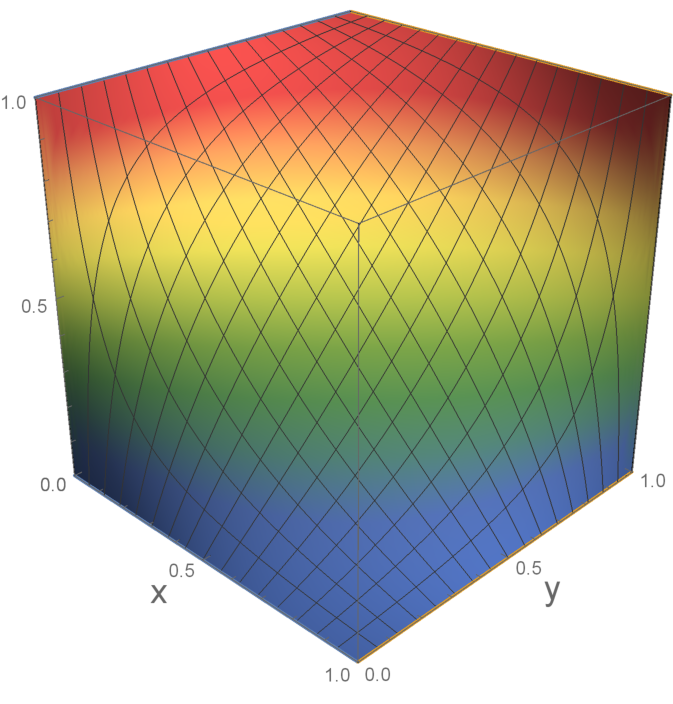
\includegraphics[width=.8\linewidth]{K1.pdf}
		\caption{$C=1$}
	\end{subfigure}%
	\begin{subfigure}{.3\textwidth}
		\centering
		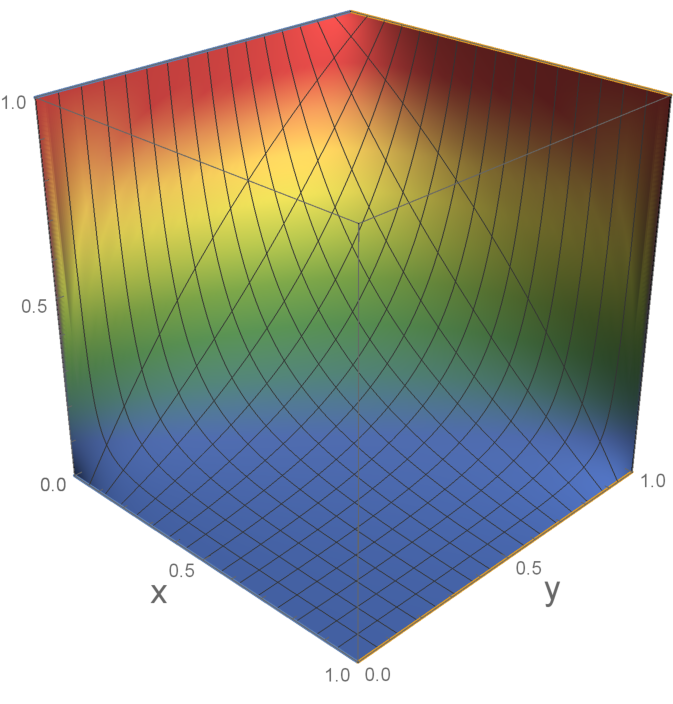
\includegraphics[width=.8\linewidth]{K10.pdf}
		\caption{$C=10$}
	\end{subfigure}
	\begin{subfigure}{.3\textwidth}
		\centering
		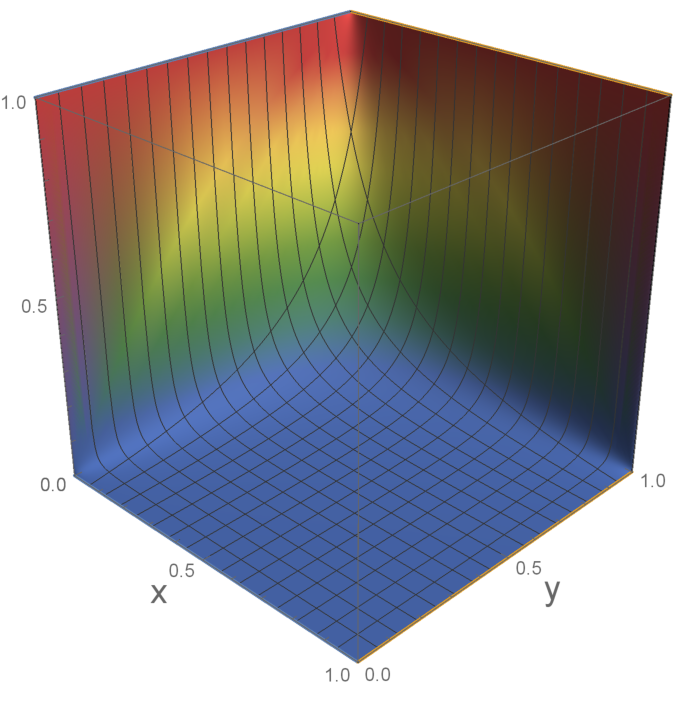
\includegraphics[width=.8\linewidth]{K100.pdf}
		\caption{$C=100$}
	\end{subfigure}
	\caption[Plots of three strict $T$-power invariant implications that satisfy \EP.]{Plots of fuzzy implication functions given in Example \ref{example:strict:(EP)} for $C=1$, $C=10$ and $C=100$.}
	\label{exfig:strict:(EP)}
\end{figure}
% Law of importation %
We now turn to study the law of importation. It is well known, that \LI implies \EP but the reverse implication does not hold in general. Thus, to study \LI we can use as starting point the five configurations in Proposition \ref{prop:strict:(EP)}. Before characterizing all strict $T$-power implications satisfying \LI let us prove the following lemma which remarks some interesting properties such as if \IT satisfies \LI with respect to some t-norm $T^*$, then $\IT$ is constant in $(0,1)^2$, $g$ is idempotent in its image except for 0 and 1 (see Lemma \ref{lem:idempotentfunctions} for a characterization of these type of functions) and if $\IT$ has trivial 1-region then necessarily $T^*$ is a positive t-norm (also called t-norm without zero-divisors), i.e., $T^*(x,y)=0$ if and only if $x=0$ or $y=0$.
% law of importation %
\begin{lemma}\label{lem:strict:(LI)} Let \IT be a \STP that satisfies \LI with respect to some t-norm $T^*$. The following statements hold:
	\begin{enumerate}[label=(\roman*)]
		\item $\IT$ is constant in $(0,1)^2$.
		\item If $\IT(x,y)=1 \Leftrightarrow (x=0 \text{ or } y=1$), then $T^*$ is a positive t-norm.
		\item $g(y)=y$ for all $y \in \Ima g\setminus \{0,1\}$.
	\end{enumerate}
\end{lemma}
\begin{proof} \hspace{0.5cm}
	\begin{enumerate}[label=(\roman*)]
		\item Let us prove that Case (i) in Proposition \ref{prop:strict:(EP)} does not satisfy \LI with respect to any t-norm $T^*$. Consider $x=1$, $y,z \in (0,1)$, we have that
		$$\IT(T^*(1,y),z)=\IT(y,z)\in(0,1),$$
		$$\IT(1,\IT(y,z))=g(\IT(y,z))=0.$$
		Thus, observing that all the other cases in Proposition \ref{prop:strict:(EP)} correspond to fuzzy implication functions which are constant in $(0,1)^2$ we obtain the result.
		\item Consider that there exist $x_0, y_0 \in (0,1)$ such that $T^*(x_0,y_0)=0$, then for $z_0 \in (0,1)$ we have that
		$$\IT(T^*(x_0,y_0),z_0)=\IT(0,z_0)=1,$$
		$$\IT(x_0,\IT(y_0,z_0))<1.$$
		Then, we arrive to contradiction with the fact that $\IT$ satisfies \LI with respect to $T^*$.
		\item Let us assume $x=y=1$ and $z \in (0,1)$, then
		\begin{eqnarray*}
		\IT(1,\IT(1,z)) &=&
		\left\{ \begin{array}{ll}
			\IT(1,0)&\text{if }z=0, \\[3pt]
			\IT(1,g(z))&\text{if }z \in (0,1),\\[3pt]
			\IT(1,1)&\text{if }z=1,
		\end{array}
		\right. \\
		&=&
		\left\{ \begin{array}{ll}
			0&\text{if }z=0 \text{ or } (z \in (0,1) \text{ and } g(z)=0), \\
			g \circ g(z)&\text{if }z \in (0,1) \text{ and } g(z) \in (0,1),\\
			1&\text{if }z=1 \text{ or } (z \in(0,1) \text{ and } g(z)=1).
		\end{array}
		\right.
		\end{eqnarray*}
		$$
		\IT(T^*(1,1),z)
		=
		\IT(1,z)
		=
		\left\{ \begin{array}{ll}
			0&\text{if }z=0, \\
			g(z)&\text{if }z \in (0,1),\\
			1&\text{if }z=1.
		\end{array}
		\right.
		$$
		Then, since $\IT$ satisfies \LI with respect to $T^*$, necessarily we have that $g\circ g(z)=g(z)$ for all $g(z) \in (0,1)$ with $z \in (0,1)$, that is equivalent to $g(y)=y$ for all $y \in \Ran g \setminus \{0,1\}$.
	\end{enumerate}
\end{proof}
Thanks to the above, the following proposition determines the three possibles configurations of strict $T$-power invariant implications that satisfy the law of importation with respect to some t-norm.
\begin{proposition}\label{prop:strict:(LI)} Let \IT be a \STP and $T^*$ a t-norm. Then $\IT$ satisfies \LI with respect to $T^*$ if and only if one of the following conditions hold:
	\begin{enumerate}[label=(\roman*)]
		\item $\varphi(w)=0$ for all $w \in (0,+\infty)$, $f(x)=g(y)=0$ for all $x,y \in (0,1)$ and $T^*$ is a positive t-norm.
		\item  Let $k \in (0,1]$, then $\varphi(w)=k$ for all $w \in (0,+\infty)$, $g(y)=y$ for all $y \in \Ima g \setminus \{0,1\}$, and one of the following conditions hold:
		\begin{enumerate}
			\item $f(x)=\left\{ \begin{array}{ll}
				k &   \text{if }   x \in A, \\
				0 &  \text{if }   x \in (0,1)\setminus A,	\end{array}
			\right.$ where $A$ is $(0,a|$ with $ a \in (0,1)$ or $A=\emptyset$, $T^*$ satisfies the following property
			$$T^*(x,y) \in (0,1]\setminus A \text{ if and only if } x,y \in (0,1]\setminus A$$
			and $\Ima g \subseteq (0,k]$.
			\item $0 \not \in \Ima f$, $f(x)=k$ for all $x \in \Ima T^*|_{(0,1)^2} \setminus \{0\}$, $g(y)=y$ for all $y \in \Ima f \setminus \{1\}$ and $\Ima g \subseteq [0,k]$ but $g(y) > 0$ for all $y \in (0,1)$ when $f$ is not a function constant to $k$.
		\end{enumerate}
		Moreover, if $k < 1$, $g$ must additionally satisfy $g(k)=k$ and $T^*$ must be a positive t-norm.
	\end{enumerate}
\end{proposition}
\begin{proof}
	Let \IT be a \STP which satisfies \LI with respect to a t-norm $T^*$. {By (i)-Lemma~\ref{lem:strict:(LI)}} we know that there exists some $k \in [0,1]$ such that $\varphi(w)=k$ for all $w \in (0,+\infty)$ and by (iii) that $g$ is idempotent in $\Ima g \setminus \{0,1\}$. Now, since we know that \LI $\Rightarrow$ \EP, then we only need to consider Cases (ii), (iii)-(a), (iii)-(b) and (iii)-(c) in Proposition \ref{prop:strict:(EP)}:
	\begin{description}
		\item[ Case (ii)] If $k=0$ we are in Case (i) of Proposition \ref{prop:strict:(LI)}. On the other hand, if $k \in (0,1]$ then \IT does not verify \LI with respect to any t-norm $T^*$ because for $x,z \in (0,1)$ we have that
		$$ \IT(T^*(x,1),z)=\IT(x,z)=k,$$
		$$\IT(x,\IT(1,z))=\IT(x,g(z))=\IT(x,0)=f(x)=0.$$
		\item[Case (iii)-(a)] Let us prove that in this case $T^*(x,y) \in (0,1] \setminus A \Leftrightarrow x,y \in (0,1] \setminus A$. Consider $x,y \in (0,1)\setminus A$ such that $T^*(x,y) \in A \cup \{0\}$, we have that
		$$\IT(T^*(x,y),0)=\left\{ \begin{array}{ll}
			k &   \text{if }   T^*(x,y) \in A, \\
			1 &  \text{if }   T^*(x,y)=0,	\end{array}
		\right. $$
		$$\IT(x,\IT(y,0))=\IT(x,0)=0,$$
		and we arrive to contradiction with the fact that $\IT$ satisfies \LI with respect to $T^*$. 		
		On the other hand, consider $T^*(x,y)\in (0,1]\setminus A$. Since $T^*(x,y) \leq \min\{x,y\}$ we have that $x,y \in (0,1] \setminus A$. This situation corresponds to (ii)-(a) in Proposition \ref{prop:strict:(LI)}.
		\item[Case (iii)-(b)] Notice that this case is contemplated in situation (ii)-(b) in Proposition \ref{prop:strict:(LI)}.
		\item[Case (iii)-(c)]  Let us prove that in this case $f(x)=k$ for all $x \in \Ima T^*|_{(0,1)^2} \setminus \{0\}$. Consider an $r \in \Ima T^*|_{(0,1)^2} \setminus \{0\}$ such that $T^*(x_0,y_0)=r$ with $(x_0,y_0)\in (0,1)^2$ and $f(r)<k$, then
		$$\IT(T^*(x_0,y_0),0)=f(T^*(x_0,y_0))=f(r)<k,$$
		$$\IT(x_0,\IT(y_0,0))=\IT(x_0,f(y_0))=k,$$
		which contradicts the fact that \IT satisfies \LI with respect to $T^*$. This situation corresponds to Case (ii)-(b) in Proposition \ref{prop:strict:(LI)}.
	\end{description}
	For the reverse implication, we have to prove that fuzzy implication functions described in (i), (ii)-(a) and (ii)-(b) satisfy \LI with respect to $T^*$. Since this step involves some tedious expressions, here we only present the details for Case (ii)-(b). Let $\varphi$, $f$, $g$ and $T^*$ fulfill conditions in (ii)-(b), then
	\begin{eqnarray*}
		\IT(T^*(x,y),z)&=&
		\left\{ \begin{array}{ll}
			0 &   \text{if }  T^*(x,y)=1 \text{ and } z=0, \\
			f(x) &  \text{if } x \in (0,1), y=1 \text{ and } z=0,\\
			f(y) & \text{if } x=1, y \in (0,1) \text{ and } z=0\\
			f(T^*(x,y)) & \text{if }x,y \in (0,1), T^*(x,y) \in (0,1) \text{ and } z=0,\\
			g(z) & \text{if } T^*(x,y)=1 \text{ and } z \in (0,1),\\
			1 & \text{if } T^*(x,y)=0 \text{ or } z =1,\\
			k & \text{otherwise,}
		\end{array} \right. \\
		&=&
		\left\{ \begin{array}{ll}
			0 &   \text{if }  x=y=1 \text{ and } z=0, \\
			f(x) &  \text{if } x \in (0,1), y=1 \text{ and } z=0,\\
			f(y) & \text{if } x=1, y \in (0,1) \text{ and } z=0,\\
			f(T^*(x,y)) & \text{if }x,y \in (0,1), T^*(x,y) \in (0,1) \text{ and } z=0,\\
			g(z) & \text{if } x=y=1 \text{ and } z \in (0,1),\\
			1 & \text{if } T^*(x,y)=0 \text{ or } z =1,\\
			k & \text{otherwise.}
		\end{array} \right.
	\end{eqnarray*}
	Let us distinguish two cases depending on the value of $k$:
	\begin{itemize}
		\item 	If $k \in (0,1)$ then
		\begin{eqnarray*}
			\IT(x,\IT(y,z)) &=&
			\left\{ \begin{array}{ll}
				\IT(x,0) &   \text{if }  y=1 \text{ and } z=0, \\[5pt]
				\IT(x,f(y)) &  \text{if } y \in (0,1) \text{ and } z=0,\\[5pt]
				\IT(x,g(z)) & \text{if } y=1 \text{ and } z \in (0,1),\\[5pt]
				\IT(x,1) & \text{if }y=0 \text{ or } z=1,\\
				k & \text{otherwise,}
			\end{array} \right. \\
			&=&
			\left\{ \begin{array}{ll}
				0 &   \text{if }  x=y=1 \text{ and } z=0, \\
				f(x) & \text{if }x\in(0,1), y=1 \text{ and } z=0, \\
				g \circ f(y) &  \text{if } x=1, y \in (0,1) \text{ and } z=0,\\
				g \circ g(z) & \text{if } x=y=1 \text{ and } z \in (0,1),\\
				1 & \text{if }x=0 \text{ or } y=0 \text{ or } z=1,\\
				k & \text{otherwise,}
			\end{array} \right. \\
			&=&
			\left\{ \begin{array}{ll}
				0 &   \text{if }  x=y=1 \text{ and } z=0, \\
				f(x) & \text{if }x\in(0,1), y=1 \text{ and } z=0, \\
				f(y) &  \text{if } x=1, y \in (0,1) \text{ and } z=0,\\
				g(z) & \text{if } x=y=1 \text{ and } z \in (0,1),\\
				1 & \text{if }x=0 \text{ or } y=0 \text{ or } z=1,\\
				k & \text{otherwise.}
			\end{array} \right.		 
		\end{eqnarray*}
		Since in this case we have that $g(k)=k$ and $T^*$ is a positive t-norm it is clear by the conditions in (ii)-(b) that \LI holds.	
		\item $k=1$
		\begin{eqnarray*}
			\IT(x,\IT(y,z)) &=&
			\left\{ \begin{array}{ll}
				0 & \text{if } (x=y=1,~ z=0) \text{ or } (x=y=1,~ g(z)=0),\\
				f(x) & \text{if } x \in (0,1), y=1 \text{ and } z=0, \\
				g \circ f(y) &   \text{if }  x=1, f(y)\in(0,1) \text{ and } z=0, \\
				g \circ g(z) &  \text{if } x=y=1 \text{ and } g(z) \in (0,1),\\
				1 & \text{otherwise,}
			\end{array} \right. \\
			&=&
			\left\{ \begin{array}{ll}
				0 &   \text{if }  x=y=1 \text{ and } z=0, \\
				f(x) & \text{if }x\in(0,1), y=1 \text{ and } z=0, \\
				f(y) &  \text{if } x=1, y \in (0,1) \text{ and } z=0,\\
				g(z) & \text{if } x=y=1 \text{ and } z \in (0,1),\\
				1 & \text{otherwise.}
			\end{array} \right.		 
		\end{eqnarray*}
		In this case also by the conditions in (ii)-(b) it is clear that \LI holds.
	\end{itemize}
\end{proof}
% Example -- (LI) %
\begin{example} Let us consider $\varphi(w)=\frac{1}{2}$ for all $w \in (0,+\infty)$, $f(x)=0$ for all $x \in (0,1)$ and
	$$
	g(y)=\left\{ \begin{array}{ll}
		y &   \text{if }   y \in \left(0,\frac{1}{4}\right), \\[3pt]
		\frac{1}{4} &  \text{if }   y \in \left[\frac{1}{4},1\right).
	\end{array}
	\right.$$
	The corresponding \STP is
	\begin{equation*}
		I^T_{\varphi,f,g}(x,y) =\left\{ \begin{array}{ll}
			0 &  \text{if }  x \in (0,1] \text{ and } y=0, \\[3pt]
			y &   \text{if }   x=1 \text{ and } y \in \left(0,\frac{1}{4}\right), \\[3pt]
			\frac{1}{4} &  \text{if }  x=1 \text{ and } y \in \left[\frac{1}{4},1\right), \\[3pt]
			1 &  \text{if }  x=0 \text{ or } y=1, \\[3pt]
			\frac{1}{2} &  \text{otherwise}.
		\end{array}
		\right.
	\end{equation*}
	Since we are in Case (ii)-(a) of Proposition \ref{prop:strict:(LI)} with $A=\emptyset$ and we can affirm that \IT satisfies the law of importation with respect to any positive t-norm, for instance the minimum t-norm \TM or the product t-norm \TP.
\end{example}

Notice that fuzzy implication functions in Case (ii)-(a) of Proposition \ref{prop:strict:(LI)} satisfy the law of importation with respect to a t-norm $T^*$ whenever the following condition holds:
\begin{equation}
	T^*(x,y) \in (0,1] \setminus A \text{ if and only if } x,y \in (0,1] \setminus A,
	\label{eq:condition_(LI)}
\end{equation}
where $A$ can be the interval $(0,a]$ or $(0,a)$ with $a \in (0,1)$ or $A=\emptyset$. In order to characterize these t-norms we study when does a t-norm satisfy Condition (\ref{eq:condition_(LI)}). Observe that if $A=\emptyset$ then $T^*$ satisfies Condition (\ref{eq:condition_(LI)}) if and only if $T^*$ is a positive t-norm. Now, the next result shows that when $A=(0,a)$, $T^*$ satisfies Condition (\ref{eq:condition_(LI)}) if and only if $a$ is an idempotent element of $T^*$.
% law of importation -- continuous case %
\begin{lemma}\label{lem:(LI)Tcont(1)}
	Let $T^*$ be a t-norm and $a\in(0,1)$. Then, {\normalfont(}$T^*(x,y) \in [a,1] \Leftrightarrow x,y \in [a,1]${\normalfont)} if and only if $a$ is an idempotent element of $T^*$.
\end{lemma}
\begin{proof}\hspace{0.5cm}
	\begin{itemize}
		\item[($\Rightarrow$)] $T^*(a,x) \leq \min\{a,x\} \leq a \Rightarrow T^*(a,x) \in [0,a]$ for all $x \in [0,1]$. Then, $T^*(a,a)\in [0,a]\cap[a,1] \Rightarrow T^*(a,a)=a$.
		\item[($\Leftarrow$)] Consider $T^*(x,y) \in [a,1]$ with $x \in [0,a)$, then
		$$T^*(x,y) \leq \min\{x,y\} \leq x < a, \quad \text{for all } y \in [0,1].$$
		This is a contradiction with the fact that $T^*(x,y) \in [a,1]$. For the reverse implication, consider $x,y \in [a,1]$. Since $a$ is an idempotent element of $T^*$ we have that
		$$T^*(x,y) \geq T^*(a,a)=a \Rightarrow T^*(x,y)\in [a,1].$$
	\end{itemize}
\end{proof}
We now consider the case when $A=(0,a]$, which presents some differences with respect to the previous case. First, we prove that if we consider a continuous t-norm $T^*$ then $T^*$ fulfills Condition (\ref{eq:condition_(LI)}) if and only if $T^*$ is the ordinal sum of two continuous t-norms, one of them positive.
\begin{lemma}\label{lem:(LI)Tcont(2)}
	Let $T^*$ be a continuous t-norm and $a \in (0,1)$. Then, {\normalfont(}$T^*(x,y) \in (a,1] \Leftrightarrow x,y \in (a,1]${\normalfont)} if and only if $T=\langle (0,a,T_1),(a,1,T_2)\rangle$ where $T_1, T_2$ are continuous t-norms and $T_2$ is also positive.
\end{lemma}
\begin{proof}
	\begin{itemize}
		\item[$(\Rightarrow)$] Let us consider $T^*$ a continuous t-norm such that $T^*(x,y) \in (a,1] \Leftrightarrow x,y \in (a,1]$. In this case
		$$T^*(x,x) >a, \quad \text{for all } x \in (a,1],$$
		and since $T^*$ is continuous, we have that
		$$T^*(a,a)=\lim_{x \to a^+} T(x,x) \geq a.$$
		On the other hand, $T(a,a) \leq \min\{a,a\} =a$. Then $T^*(a,a)=a$ and $a$ is an idempotent element. By the characterization of continuous t-norms we know that $T=\langle (0,a,T_1),(a,1,T_2)\rangle$ with $T_1$ and $T_2$ continuous t-norms. Now, let us see that $T_2$ needs to be a positive t-norm. If there exists $x_0,y_0 \in (0,1)$ with $T_2(x_0,y_0)=0$, we define $x=a+(1-a)x_0$ and $y=a+(1-a)y_0$ with $x,y \in(a,1]$. Then,
		$$T^*(x,y)=a+(1-a)T_2 \left(\frac{x-a}{1-a},\frac{y-a}{1-a}\right)=a+(1-a)T_2(x_0,y_0)=a,$$
		and we arrive to contradiction with the fact that $T^*(x,y) \in (a,1] \Leftrightarrow x,y \in (a,1]$.
		\item[$(\Leftarrow)$] Consider $T^*(x,y) \in (a,1]$ and $x \in [0,a]$, then
		$$T^*(x,y) \leq \min\{x,y\} \leq x \leq a, \quad \text{for all } y \in [0,1].$$
		Contradiction with $T^*(x,y) \in (a,1]$. On the other hand, if $x,y \in (a,1]$ then $x_0=\frac{x-a}{1-a}$ and $y_0=\frac{y-a}{1-a}$ are such that $x_0,y_0 \in (0,1]$. Thus $T_2(x_0,y_0)>0$ and
		$$T(x,y)=a+(1-a)T_2\left(\frac{x-a}{1-a},\frac{y-a}{1-a}\right)=a+(1-a)T_2(x_0,y_0)>a. \vspace{-0.5cm}$$ \qedhere
	\end{itemize}
\end{proof}
Notice that the proof of the previous lemma relies on the characterization of continuous t-norms. It is well known that a similar characterization for non-continuous t-norms is not available, which makes solving the problem of Lemma \ref{lem:(LI)Tcont(2)} in the non-continuous case a hard challenge. Moreover, notice that in this case a similar result to Lemma \ref{lem:(LI)Tcont(1)} is not true when $T^*$ is not continuous. For instance, the following family of non-continuous t-norms (see \cite[Proposition 3.66]{Klement2000}):
$$
T_{[0,a],b}(x,y)=
\left\{ \begin{array}{ll}
	0 &   \text{if }   x,y \in [0,a], \\
	b &  \text{if }   x,y \in (a,1], \\
	\min\{x,y\} & \text{otherwise,}
\end{array}
\right.
$$
with $b \in (a,1]$, satisfies Condition (\ref{eq:condition_(LI)}) with $A=(0,a]$ but these t-norms do not have $a$ as an idempotent element.\\
Having said this,  for continuous t-norms we can rewrite Proposition \ref{prop:strict:(LI)} into the following corollary.
\begin{corollary}\label{cor:(LI)Tcont} Let $\IT$ be a strict $T$-power invariant implication and $T^*$ a continuous t-norm. Then $\IT$ satisfies \LI with respect to $T^*$ if and only if one of the following conditions hold:
	\begin{enumerate}[label=(\roman*)]
		\item $\varphi(w)=0$ for all $w \in (0,+\infty)$, $f(x)=g(y)=0$ for all $x,y \in (0,1)$ and $T^*$ is a positive t-norm.
		\item  Let $k \in (0,1]$, then $\varphi(w)=k$ for all $w \in (0,+\infty)$, $g(z)=z$ for all $z \in \Ima g \setminus \{0,1\}$ and one of the following conditions hold:
		\begin{enumerate}
			\item $f(x)=0$ for all $x \in (0,1)$, $\Ima g \subseteq (0,k]$ and $T^*$ is positive.
			\item $f(x)=\left\{ \begin{array}{ll}
				k &   \text{if }   x \in A, \\
				0 &  \text{if }   x \in (0,1)\setminus A,	\end{array}
			\right.$ where $A$ is $(0,a|$ with $ a \in (0,1)$, $\Ima g \subseteq (0,k]$ and $T^*=\langle (0,a,T_1),(a,1,T_2) \rangle$ where $T_1,T_2$ are continuous t-norms and $T_2$ is positive whenever $A=(0,a]$.
			\item $0 \not \in \Ima f$, $f(x)=k$ for all $x \in \Ima T^*|_{(0,1)^2} \setminus \{0\}$ and $\Ima g \subseteq [0,k]$ but $g(y) > 0$ for all $y \in (0,1)$ when $f$ is not a function constant to $k$.
		\end{enumerate}
		Moreover, if $k < 1$, $g$ must additionally satisfy that $g(k)=k$ and $T^*$ must be a positive t-norm.
	\end{enumerate}
\end{corollary}
% Iterative Boolean Law %
Next, let us consider the iterative boolean law. Similarly to the study of the two previous properties, we first provide a lemma which remarks some conditions that $f$, $g$ and $\varphi$ must satisfy when the corresponding \STP satisfies \IB. In this case, $g$ has to be idempotent in its image except for 0 and 1, $\varphi$ cannot be strictly increasing and, similarly to the case when \IT satisfies \EP, if $\varphi$ is constant to $k\in(0,1)$ in some $(a,b) \subseteq (0,+\infty)$ then $\varphi$ is indeed constant in $(0,+\infty)$.
% Iterative boolean law %
\begin{lemma}\label{lem:strict:(IB)}
	Let \IT be a \STP that satisfies \IB. Then, the following properties hold:
	\begin{enumerate}[label=(\roman*)]
		\item $g(y)=y$ for all $y \in \Ima g \setminus \{0,1\}$.
		\item $\varphi$ is not strictly increasing.
		\item If there exists a constant $k \in (0,1)$ and an interval $(a,b)$ with $a,b \in (0,+\infty)$ and $a<b$ such that $\varphi(w)=k$ for all $w \in (a,b)$, then $\varphi(w)=k$ for all $w \in (0,+\infty)$.
	\end{enumerate}
\end{lemma}
\begin{proof} Let \IT be a \STP that satisfies \IB.
	\begin{enumerate}[label=(\roman*)]
		\item Consider $x=1$ and $y \in (0,1)$ such that $g(y) \in (0,1)$, then
		$$ \IT(1,y)=g(y),$$
		$$ \IT(1,\IT(1,y))=\IT(1,g(y))=g \circ g (y),$$
		and the result follows.
		\item Let $\varphi$ be a strictly increasing function. Consider $x \in (0,1)$, then
		$$\varphi(1)=\IT(x,x)=\IT(x,\IT(x,x))=\IT(x,\varphi(1))=\varphi \left(\frac{t(x)}{t \circ \varphi(1)}\right).$$
		Now, since $\varphi$ is strictly increasing we obtain that $t(x)=t\circ \varphi (1)$ for all $x\in (0,1)$ which contradicts the fact that $t$ is a generator of a strict t-norm.
		\item  	Fix a $y_0 \in (0,1)$, we have that
		$$ \varphi \left(\frac{t(x)}{t(y_0)}\right)=k, \quad \text{for all } x \in (t^{-1}(bt(y_0)),t^{-1}(at(y_0))).$$
		Now, since $\IT$ verifies \IB we get
		\begin{eqnarray*}
		k &= & \varphi\left(\frac{t(x)}{t(y_0)}\right)=\IT(x,y_0)=\IT(x,\IT(x,y_0))=\IT\left(x,\varphi\left(\frac{t(x)}{t(y_0)}\right)\right) \\
		&=& \IT(x,k)=\varphi\left(\frac{t(x)}{t(k)}\right),
		\end{eqnarray*}
		and $\varphi(w)=k$ for all $w \in \frac{t(y_0)}{t(k)}(a,b)$. Now, with  an analogous proof to the one provided in Lemma \ref{lem:strict:phi_const}, we prove that $\varphi(w)=k$ for all $w \in (0,+\infty)$. \qedhere
	\end{enumerate}
\end{proof}
Taking into account the lemma above, we now characterize the only two possible structures of strict $T$-power implications that satisfy \IB.
\begin{proposition}\label{prop:strict:(IB)} Let \IT be a \STP. Then \IT satisfies \IB if and only if one of the following conditions hold:
	\begin{enumerate}[label=(\roman*)]
		\item $\Ima \varphi  \subseteq \{0,1\}$, $\varphi$ is not constant to 1 and $f(x)=g(y)=0$ for all $x,y \in (0,1)$.
		\item Let $k \in (0,1]$, then $\varphi(w)=k$ for all $w \in (0,+\infty)$, $\Ima f \subseteq \{0,k\}$, $\Ima g \subseteq [0,k]$ and $g(y)=y$ for all $y \in \Ima g \setminus \{0,1\}$.
	\end{enumerate}
\end{proposition}
\begin{proof}
	Let \IT be a \STP which satisfies \IB, by {(ii)-Lemma~\ref{lem:strict:(IB)}} we know that $\varphi$ is not strictly increasing, then there exists a constant $k\in [0,1]$ and an interval $(a,b)$ with $a,b \in (0,+\infty)$ and $a<b$ such that $\varphi(w)=k$ for all $w\in (a,b)$. Let us distinguish three cases depending on the possible values of $k$:
	\begin{enumerate}
		\item If $k \in (0,1)$, then by {(iii)-Lemma~\ref{lem:strict:(IB)}} we know that $\varphi(w)=k$ for all $w \in (0,+\infty)$ and by {(i)-Lemma~\ref{lem:strict:(IB)}} we have that $g(z)=z$ for all $z \in \Ima g \setminus \{0,1\}$. By Condition (\ref{eq:strict:TPowerInv:MonotonicityCond}), $\Ima f \subseteq [0,k]$ and $\Ima g \subseteq [0,k]$. Now, consider an $x \in (0,1)$ such that $f(x) \in (0,k)$, then since \IT satisfies \IB
		$$f(x)=\IT(x,0)=\IT(x,\IT(x,0))=\IT(x,f(x))=k,$$
		and we arrive to a contradiction. Thus, $\Ima f \subseteq \{0,k\}$.
		\item If $k=0$, then since $\varphi$ is increasing we have that $\varphi(w)=0$ for all $ w\in [0,b)$. By {(i)-Proposition~\ref{prop:strict:continuity}} we know that $f(x)=g(y)=0$ for all $x,y \in (0,1)$. Now, let us assume that there exists a $w_0 \in (0,+\infty)$ such that $\varphi(w_0) \in (0,1)$. Consider $x_0,y_0 \in (0,1)$ such that $x_0 > t^{-1}(b\cdot t \circ \varphi (w_0))$ and $y_0=t^{-1}\left(\frac{t(x_0)}{w_0}\right)$, then
		$$\IT(x_0,y_0)=\varphi(w_0) \in (0,1),$$
		$$\IT(x_0,\IT(x_0,y_0))=\IT(x_0,\varphi(w_0))=\varphi \left(\frac{t(x_0)}{t \circ \varphi(w_0)}\right)=0,$$
		which contradicts the fact that \IT satisfies \IB. Then, $\Ima \varphi \subseteq \{0,1\}$.
		\item If $k = 1$, then since $\varphi$ is increasing we have that $\varphi(w)=1$ for all $w \in (a,+\infty]$. If $\varphi(w_0)=0$ for some $w_0 \in(0,a]$ we are in the same situation of the previous point so let us assume that $\varphi(w) \in (0,1]$ for all $w \in (0,+\infty)$. Now, consider that there exists a $w_0 \in (0,a]$ with $\varphi(w_0) \in (0,1)$. Let us choose $x_0,y_0 \in (0,1)$ such that $x_0 < t^{-1}(a\cdot t \circ \varphi (w_0))$ and $y_0=t^{-1} \left(\frac{t(x_0)}{w_0}\right)$, then
		$$ \IT(x_0,y_0) = \varphi(w_0) \in (0,1),$$
		$$\IT(x_0,\IT(x_0,y_0))=\IT(x_0,\varphi(w_0))=\varphi \left(\frac{t(x_0)}{t \circ \varphi (w_0)}\right) = 1,$$
		which contradicts the fact that \IT satisfies \IB. Then, in this case, $\varphi(w)=1$ for all $w \in (0,+\infty)$. Now, let us assume that there exists an $x_0 \in (0,1)$ such that $f(x_0) \in (0,1)$. Then, on the one hand, $\IT(x_0,0)=f(x_0)$ and, on the other hand,
		$$\IT(x_0,\IT(x_0,0))=\IT(x_0,f(x_0))=1,$$
		and we arrive to contradiction with the fact that $\IT$ satisfies \IB. Thus, $\Ima f \subseteq \{0,1\}$.
	\end{enumerate}
	For the reverse implication we have to prove that fuzzy implication functions (i) and (ii) in Proposition \ref{prop:strict:(IB)} satisfy \IB.	Since this verification is similar to previous proofs we do not specify the details.
\end{proof}
% Example -- (IB) %
\begin{example}\label{example:strict:(IB)} Let $T$ be any strict t-norm, $t$ an additive generator of $T$, $f(x)=g(y)=0$ for all $x,y\in(0,1)$ and
	$$\varphi(w)= \left\{ \begin{array}{ll}
		0 &   \text{if }   w < \frac{1}{a}, \\
		1 &  \text{otherwise}, 	\end{array}
	\right.
	$$	
	with $a \in (0,+\infty)$. Then, the corresponding strict $T$-power invariant implication
	\begin{equation*}
		I^T_{\varphi,f,g}(x,y) =\left\{ \begin{array}{ll}
			0 & \text{if }  y<t^{-1}(at(x)),\\
			1 &  \text{otherwise},
		\end{array}
		\right.
	\end{equation*}
	satisfies the iterative boolean law.
\end{example}

Finally, we study when a strict $T$-power invariant implication satisfies \TC with respect to $T$. However, first of all let us point out some general facts about the $T$-conditionality. Let $T$ be a t-norm, since $T(x,y) \leq x$ for all $x,y \in [0,1]$, it is straightforward to see that for a given fuzzy implication function $I$, if $x \leq y$, then $T(x,I(x,y))\leq x \leq y$. Hence, it actually suffices to consider only the cases $x>y$ when studying \TC. Moreover, the following result follows.
\begin{proposition}\label{prop:(TC)&LowTrianZero}
	Let $I$ be a fuzzy implication function such that $I(x,y)=0$ for all $x>y$, then $I$ satisfies \TC with any t-norm $T$.
\end{proposition}
\begin{proof}
	Let us consider $x,y \in [0,1]$ with $x>y$, then $T(x,I(x,y))=T(x,0)=0 \leq y$.
\end{proof}
In fact, the previous proposition gives a construction method for obtaining a fuzzy implication function that satisfies \TC with any t-norm $T$ by only replacing the values $x,y \in [0,1]$, $x>y$ with zero.
\begin{proposition}\label{prop:(TC):Completing0s}
	Let $I$ be a fuzzy implication function. Then $I':[0,1]^2 \to [0,1]$ given by
	\begin{eqnarray*}
		I'(x,y) 
		&=&
		\left\{ \begin{array}{ll}
			I(x,y) & \text{if } x \leq y,\\
			0 	   & \text{if }   x>y,			
		\end{array}
		\right.
	\end{eqnarray*}
	is a fuzzy implication function that satisfies \TC with any t-norm $T$.
\end{proposition}
It is true that Proposition \ref{prop:(TC):Completing0s} gives a construction method for obtaining a fuzzy implication function satisfying \TC with respect to any t-norm from another fuzzy implication function. However, it is clear that this is not a very interesting method since it eliminates too much information from the original fuzzy implication function. Unfortunately, with respect to strict $T$-power invariant implications, the next proposition proves that \IT satisfies \TC with respect to $T$ if a only if $\IT(x,y)=0$ for all $x >y$. Thus, for this family of fuzzy implication functions only trivial solutions satisfy \TC with respect to $T$.
\begin{proposition}\label{prop:strict:(TC)}
	Let \IT be a strict $T$-power invariant implication. Then \IT satisfies  \TC with respect to $T$ if and only if $\varphi(w)=0$ for all $w \in [0,1)$, and $f(x)=g(y)=0$ for all $x,y \in (0,1)$. In this case, \IT satisfies \TC with respect to any t-norm $T^*$.
\end{proposition}
\begin{proof}
	\begin{itemize}
		\item[$(\Rightarrow)$] Let \IT be a strict $T$-power invariant implication and $t$ an additive generator of $T$. Let us assume that there exists a $\tilde{w} \in (0,1)$ such that $\varphi(\tilde{w})>0$. Since
		$$\lim_{ y \to 0^+}  t^{-1}((1-\tilde{w})t(y))=0,$$
		there exists $\tilde{y} \in (0,1)$ such that $\varphi(\tilde{w}) > t^{-1}((1-\tilde{w})t(\tilde{y}))>0$. Moreover, since \linebreak $\left\{\frac{t(x)}{t(\tilde{y})} \mid x \in (0,1)\right\} = (0,+\infty)$ there exists an $\tilde{x} \in (\tilde{y},1)$ such that $\tilde{w}=\frac{t(\tilde{x})}{t(\tilde{y})}$. In this case,
		\begin{eqnarray*}
			\varphi(\tilde{w})>t^{-1}(t(\tilde{y})(1-\tilde{w})) & \Rightarrow &  \varphi\left(\frac{t(\tilde{x})}{t(\tilde{y})}\right)>t^{-1}\left(t\left(\tilde{y}\right)\left(1-\frac{t(\tilde{x})}{t(\tilde{y})}\right)\right)\\
			& \Rightarrow &  \varphi\left(\frac{t(\tilde{x})}{t(\tilde{y})}\right)>t^{-1}\left(t(\tilde{y})-t(\tilde{x})\right) \\
			& \Rightarrow &  t(\tilde{x}) + t\left(\varphi\left(\frac{t(\tilde{x})}{t(\tilde{y})}\right)\right)<t(\tilde{y}) \\
			& \Rightarrow &  t^{-1}\left(t(\tilde{x}) + t\left(\varphi\left(\frac{t(\tilde{x})}{t(\tilde{y})}\right)\right)\right) > \tilde{y} \\
			& \Rightarrow &  T(\tilde{x},I(\tilde{x},\tilde{y})) > \tilde{y},
		\end{eqnarray*}
		and we obtain a contradiction with the fact that \IT satisfies \TC with respect to $T$. Finally, by Condition (\ref{eq:strict:TPowerInv:MonotonicityCond}) we obtain that $f(x)=g(y)=0$ for all $x,y \in (0,1)$.
		\item[$(\Leftarrow)$]  If $\varphi(w)=0$ for all $w \in [0,1)$ and $f(x)=g(y)=0$ for all $x,y \in (0,1)$ then \IT is given by 
		\begin{equation}
			I^T_{\varphi,f,g}(x,y) =\left\{ \begin{array}{ll}
				\varphi \left(\frac{t(x)}{t(y)}\right) &   \text{if }   x \leq y, \\
				0 &  \text{if }   x>y.
			\end{array}
			\right.
		\end{equation}
		Thus, the result follows by Proposition \ref{prop:(TC)&LowTrianZero}.
	\end{itemize}
\end{proof}


\begin{remark}\label{remark:strictrestrictive}
	According to the study of this section, if \IT is a \STP that satisfies \CB, \NP, \EP, \IB or \LI and we are not in Case (i) of either Proposition \ref{prop:strict:(EP)} or Proposition \ref{prop:strict:(IB)}, then \IT is constant in $(0,1)^2$. Then, notice that the expression of this fuzzy implication function is independent from the generator of the corresponding t-norm. Therefore, we get that \IT is $T$-power invariant with respect to any strict t-norm. This fact leads to conclude that imposing some additional property besides the $T$-power invariance seems to be very restrictive and usually leads to degenerated solutions. However, Case (i) in Proposition \ref{prop:strict:(EP)} might be an interesting family of fuzzy implication functions satisfying both \EP and the $T$-power invariance.
\end{remark}
\subsection{Additional properties of nilpotent $T$-power invariant implications}\label{subsection:additional_propertiesNilpotentTpower}

In this section we perform an analogous study to the previous one but for  nilpotent $T$-power invariant implications. First of all, we study the continuity of nilpotent $T$-power invariant implications. Since the structure of these fuzzy implication functions depends on the choice of three functions, it is obvious that the continuity of \IT depends completely on the continuity of $f$, $g$ and $\varphi$. Then, the following result is more a description than a revealing result.

\begin{proposition}\label{prop:nilpotent:continuity}
	Let \IT be a nilpotent $T$-power invariant implication. The following statements hold:
	\begin{enumerate}[label=(\roman*)]
		\item If $\varphi$ is continuous on $w=0$, then $g(y)=0$ for all $y \in (0,1)$.
		\item If $\displaystyle \lim_{x \to 0^+} f(x)=1$, then $\varphi(w)=1$ for all $w \in (1,+\infty)$.
		\item If $\displaystyle \lim_{y \to 1^-} g(y)=1$, then $\varphi(w)=1$ for all $w \in (0,+\infty)$.
		\item \IT is continuous on $(1,y_0)$ for $y_0 \in (0,1)$ if and only if $\displaystyle g(y_0)=\lim_{w \to 0^+} \varphi(w)$.
		\item \IT is continuous on $(x_0,1)$ for $x_0 \in (0,1)$ if and only if $\displaystyle \lim_{w \to +\infty} \varphi(w)=1$.
		\item \IT is continuous on $(0,y_0)$ for $y_0 \in (0,1)$ if and only if $\displaystyle \lim_{w \to \frac{t(0)}{t(y_0)}} \varphi(w)=1$.
		\item \IT is continuous on $(x_0,0)$ for $x_0 \in (0,1)$ if and only if $\displaystyle \lim_{w \to \frac{t(x_0)}{t(0)}} \varphi(w)=f(x_0)$. 
		\item \IT is continuous on $(x_0,y_0)$ for $x_0,y_0 \in (0,1)$ if and only if $\varphi$ is continuous on $\frac{t(x_0)}{t(y_0)}$.
	\end{enumerate}
\end{proposition}

\begin{proof} Points (i), (ii) and (iii) follow directly from Lemma \ref{lem:nilpot:monotonicity_condition:necessicity}.
	\begin{enumerate}
		\item[(iv)]  \IT is continuous on $(1,y_0)$ for $y_0 \in (0,1)$  if and only if
		$$g(y_0)=\IT(1,y_0)=\lim_{(x,y) \to (1,y_0)} \IT(x,y) = \lim_{(x,y) \to (1,y_0)} \varphi \left(\frac{t(x)}{t(y)}\right) = \lim_{w \to 0^+} \varphi(w).$$
		\item[(v)] \IT is continuous on $(x_0,1)$ for $x_0 \in (0,1)$ if and only if
		$$1=\IT(x_0,1)=\lim_{(x,y) \to (x_0,1)} \IT(x,y) = \lim_{(x,y) \to (x_0,1)} \varphi \left(\frac{t(x)}{t(y)} \right) = \lim_{w \to + \infty} \varphi(w).$$
		\item[(vi)] \IT is continuous on $(0,y_0)$ for $y_0 \in (0,1)$ if and only if 
		$$1 = \IT(0,y_0)= \lim_{(x,y) \to (0,y_0)} \IT(x,y) = \lim_{(x,y) \to (0,y_0)} \varphi \left(\frac{t(x)}{t(y)}\right) = \lim_{w \to \frac{t(0)}{t(y_0)}} \varphi(w).$$
		\item[(vii)] \IT is continuous on $(x_0,0)$ for $x_0 \in (0,1)$ if and only if 
		\begin{eqnarray*}
		f(x_0) &=& \IT(x_0,0)= \lim_{(x,y) \to (x_0,0)} \IT(x,y) = \lim_{(x,y) \to (x_0,0)} \varphi \left(\frac{t(x)}{t(y)}\right) \\
		&=& \lim_{w \to \frac{t(x_0)}{t(0)}} \varphi(w).
		\end{eqnarray*}
		\item[(viii)] \IT is continuous on $(x_0,y_0)$ for $x_0,y_0 \in (0,1)$ if and only if 
		\begin{eqnarray*}
		\varphi \left(\frac{t(x_0)}{t(y_0)}\right) &=& \IT(x_0,y_0) = \lim_{(x,y) \to (x_0,y_0)} \IT(x,y) = \lim_{(x,y) \to (x_0,y_0)} \varphi \left(\frac{t(x)}{t(y)}\right) \\
		&=& \lim_{w \to \frac{t(x_0)}{t(y_0)}} \varphi(w).
		\end{eqnarray*}
	\end{enumerate}
\end{proof}

With respect to continuity, one interesting property to point out is that these fuzzy implication functions are never continuous.

\begin{corollary}\label{cor:nilpotent:discontinuous}
	Let \IT be a nilpotent $T$-power invariant implication. Then \IT is discontinuous on (1,0) or (1,1).
\end{corollary}

\begin{proof}
	Assume that \IT is continuous on (1,1), then
	$$1=\IT(1,1)=\lim_{y \to 1^-} \IT(1,y)=\lim_{y \to 1^-} g(y),$$
	and by (iii)-Proposition \ref{prop:nilpotent:continuity} we know that $\IT(x,y)=1$ for all $(x,y) \in (0,1)^2$ and then \IT is not continuous on (1,0).
\end{proof}

However, differently from the strict case (see Corollary \ref{cor:strict:discontinuous}), Example \ref{ex:nilpot:TPowerInv} shows that a nilpotent $T$-power invariant implication can be simultaneously continuous on the points (1,0) and (0,0).

% NATURAL NEGATION
Similarly to the case of strict $T$-power invariant implications, for the nilpotent case it is clear that the natural negation of the fuzzy implication function is given by $f$. Then, one has the freedom of fixing the most convenient fuzzy negation as long as it respects Condition (\ref{eq:def:nilpot:TPowerInv:MonotonicityCond}). An important difference from the strict case is that now the supremum of $f$ is not necessarily fixed by the infimum of $\varphi$ (see Examples \ref{ex:nilpot:TPowerInv} and \ref{example:nilpotent:naturalnegation}).
\begin{proposition}\label{cor:nilpotent:natural_negation}
	Let \IT be a nilpotent $T$-power invariant implication. The natural negation of \IT is given by
	$$
	N_{\IT}(x)= \left\{ \begin{array}{ll}
		1 &   \text{if }   x=0, \\
		f(x) &   \text{if }   x \in (0,1), \\
		0 &  \text{if }   x=1. 	\end{array}
	\right.
	$$ 
\end{proposition}

We now provide an example that points out more differences between strict and nilpotent $T$-power invariant implications.

\begin{example}\label{example:nilpotent:naturalnegation} Let us consider the strict t-norm $T_1(x,y)=\frac{xy}{x+y-xy}$ for all $x,y \in [0,1]$ with additive generator $t_1(s)=\frac{1-s}{s}$ for all $s \in [0,1]$, the nilpotent t-norm $T_2(x,y)=\TLK(x,y)$ for all $x,y \in [0,1]$ with additive generator $t_2(s)=1-s$ for all $s \in [0,1]$, and the functions
	$$\varphi(w)= \left\{ \begin{array}{ll}
		0 &   \text{if }   w \leq \frac{1}{2}, \\
		1-\frac{1}{2w} &  \text{otherwise}, 	\end{array}
	\right. \quad g(y)=0 \text{ for all } y \in(0,1),
	$$
	$$f_1(x)=0 \text{ for all } x \in (0,1), 
	\quad 
	f_2(x)=
	\left\{ \begin{array}{ll}
		\frac{2x-1}{2(x-1)} & \text{if } x \in (0,0.5),\\
		0 & \text{if } x \in [0.5,1)
	\end{array}
	\right.
	$$
	The corresponding strict and nilpotent $T$-power invariant implications are given by
	$$
		I_{\varphi,f_1,g}^{T_1}(x,y) =\left\{ \begin{array}{ll}
			1 & \text{if } (x,y) \in \{(1,1),(0,0)\},\\
			\frac{xy+x-2y}{2(x-1)y} &  \text{if } y> \frac{x}{2-x},\\
			0 & \text{otherwise,}
		\end{array}
		\right.
	$$
	$$
		I_{\varphi,f_2,g}^{T_2}(x,y) =\left\{ \begin{array}{ll}
			1 & \text{if } (x=0 \text{ and } y \in [0,1]) \text{ or } (x \in (0,1] \text{ and } y=1),\\
			\frac{2x-1}{2(x-1)} &   \text{if }   x \in (0,0.5) \text{ and } y=0, \\
			\frac{2x-y-1}{2(x-1)} &  \text{if } y>2x-1,\\
			0 & \text{otherwise.}
		\end{array}
		\right.
	$$
	Although both fuzzy implication functions are constructed using the same function $\varphi$, in Figure \ref{exfig:nilpotent:naturalnegation} we can graphically observe two main differences between the two functions. In the nilpotent case, the function is not continuous when $x=0$, that is because we have to impose that in this boundary the implication must value 1. Moreover, in the strict case the function $f_1$ must be constant to 0 whereas in the nilpotent case the function $f_2$ is strictly decreasing on the interval $(0,0.5]$ even though the infimum of $\varphi$ is 0.
	
	\begin{figure}[H]
		\centering
		\begin{subfigure}{.5\textwidth}
			\centering
			\begin{center}
				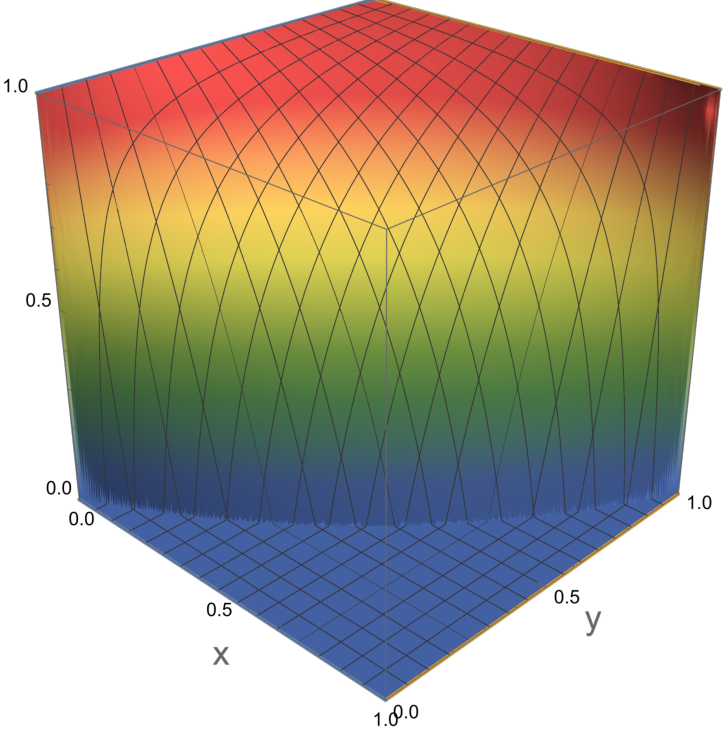
\includegraphics[width=.6\linewidth]{Example1-1.pdf}
			\end{center}
			\caption{$I_{\varphi,f_1,g}^{T_1}$~~~~~~~}
		\end{subfigure}%
		\begin{subfigure}{.5\textwidth}
			\centering
			\begin{center}
				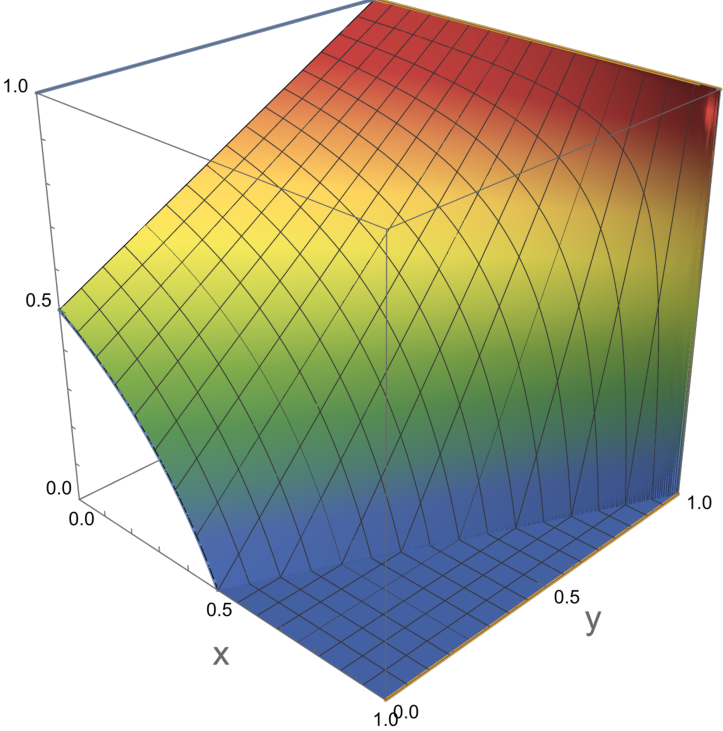
\includegraphics[width=.6\linewidth]{Example1-2.pdf}
			\end{center}
			\caption{$I_{\varphi,f_2,g}^{T_2}$~~~~~~~}
		\end{subfigure}
		\caption[Plot of a strict and a nilpotent $T$-power invariant implication.]{The strict and nilpotent $T$-power invariant implications constructed in Example \ref{example:nilpotent:naturalnegation}.}\label{exfig:nilpotent:naturalnegation}
	\end{figure}
\end{example}

% 1 - REGION  %
Next, analogously to the strict case (see Proposition~\ref{prop:strict:1-region}), we can easily construct a nilpotent $T$-power invariant implication with a trivial 1-region by choosing a function $\varphi$ strictly bounded by 1.
\begin{proposition}\label{prop:nilpotent:1-region}
	Let \IT be a nilpotent $T$-power invariant implication, then $(\IT(x,y)=1 \Leftrightarrow x=0 \text{ or } y=1)$ if and only if $\varphi(w)<1$ for all $w \in (0,+\infty)$.
\end{proposition}

\begin{proof}
	Assume that \IT satisfies that $\IT(x,y)=1 \Leftrightarrow x=0 \text{ or } y=1$. From the expression of nilpotent $T$-power invariant implications (see Equation (\ref{eq:nilpot:TPowerInv:Expression})) we obtain that if $x,y\in (0,1)$ then $\IT(x,y)=\varphi \left(\frac{t(x)}{t(y)}\right) <1$ and since $\left \{\frac{t(x)}{t(y)} \bigm| x,y \in (0,1) \right\} = (0,+\infty)$ we have that $\varphi(w)<1$ for all $w \in (0,+\infty)$. On the other hand, if $\varphi(w)<1$ for all $w \in (0,+\infty)$ then by Condition (\ref{eq:def:nilpot:TPowerInv:MonotonicityCond})  we have that $f(x),g(y)<1$ for all $x,y \in (0,1)$ and directly from Equation (\ref{eq:nilpot:TPowerInv:Expression}) we obtain that $\IT(x,y)=1 \Leftrightarrow x=0 \text{ or } y=1$.
\end{proof}


% (OP) and (IP) %

Hereunder, we characterize when the family of nilpotent $T$-power invariant implications satisfy the identity principle or the ordering property. Again, these two properties are relatively easy to study due to the fact that $I(x,x)$ is constant whenever $I$ is invariant with respect to a continuous Archimedean t-norm (\cite[Lemma 6]{Massanet2019B}).


\begin{proposition}\label{prop:nilpotent:(OP)n(IP)}
	Let \IT be a nilpotent $T$-power invariant implication. Then $\IT$ satisfies \IP if and only if $\varphi(1)=1$. In this case, $\IT$ satisfies \OP if and only if $\varphi(w)<1$ for all $w<1$.
\end{proposition}
\begin{proof}
	Since $\IT(x,x)=\PHI{x}{x} =\varphi(1)$ for all $x \in (0,1)$ it is straightforward to prove that $\IT$ satisfies \IP if and only if $\varphi(1)=1$. Now, assume that \IT satisfies \OP and consider $w \in (0,1)$, then there exist $x,y \in (0,1)$ such that $\frac{t(x)}{t(y)}=w$ and $x > y$. Therefore,
	$$\varphi(w)=\PHI{x}{y} = \IT(x,y) <1.$$
	For the reverse implication, since \IT satisfies \IP we know that $\IT(x,y)=1$ for all $x \leq y$ and since $\varphi(w)<1$ for all $w<1$ then $\IT(x,y)<1$ for all $1>x>y>0$. Finally, by \Ione and \Itwo we have that $I(x,0)<1$ for all $x \in (0,1]$ and $I(1,y)<1$ for all $y \in [0,1)$.
\end{proof}

%Consequent Boundary%

The following result deals with the study of the consequent boundary, in this case a nilpotent $T$-power invariant implication that satisfies \CB must satisfy $g(y) \geq y$ for all $y \in (0,1)$, and it is constant to 1 inside the unit square.

\begin{proposition}\label{prop:nilpot:(CB)}
	Let \IT be a nilpotent $T$-power invariant implication. Then \IT satisfies \CB if and only if $g(y) \geq y$ for all $y \in (0,1)$. Moreover, in this case \IT is given by
	\begin{equation}\label{eq:nilpot:(CB)}
		\IT(x,y) =\left\{ \begin{array}{ll}
			0 &   \text{if }   x=1 \text{ and } y=0, \\
			f(x) &  \text{if }  x \in (0,1) \text{ and } y=0, \\
			g(y) &  \text{if } x=1 \text{ and } y \in (0,1), \\
			1 & \text{otherwise.}
		\end{array}
		\right.
	\end{equation}
\end{proposition}
\begin{proof}
	Assume that $g(y) \geq y$ for all $y \in (0,1)$, then by Lemma \ref{lem:nilpot:monotonicity_condition:necessicity} we have $\varphi(w)=1$ for all $w \in(0,+\infty)$ and \IT has the structure in Equation (\ref{eq:nilpot:(CB)}). In this case, it is straightforward to verify that \IT satisfies \CB. On the other hand, if \IT satisfies \CB then by definition $g(y)=\IT(1,y)\geq y$ for all $y \in (0,1)$.
\end{proof}

% Neutrality Principle %

Now, we study the left neutrality principle. Similarly to the strict case (see Proposition \ref{prop:strict:(NP)}), a nilpotent $T$-power implication that satisfies \NP is constant to 1 in $(0,1)^2$.

\begin{proposition}\label{prop:nilpotent:(NP)}
	Let \IT be a nilpotent $T$-power invariant implication. Then \IT satisfies \NP if and only if $g(y)=y$ for all $y \in (0,1)$. Moreover, in this case \IT is given by
	\begin{equation}\label{eq:nilpot:(NP)}
		\IT(x,y) =\left\{ \begin{array}{ll}
			0 &   \text{if }   x=1 \text{ and } y=0, \\
			f(x) &  \text{if }  x \in (0,1) \text{ and } y=0, \\
			y &  \text{if } x=1 \text{ and } y \in (0,1), \\
			1 & \text{otherwise.}
		\end{array}
		\right.
	\end{equation}
\end{proposition}
\begin{proof}
	Similar to the one of Proposition \ref{prop:nilpot:(CB)}.
\end{proof}

On the other hand, similarly to the strict case (see Proposition \ref{prop:strict:(NPe)}) we obtain a solution non-constant to 1 in $(0,1)^2$ when we study the left neutrality principle with respect to an $e \in (0,1)$. However, differently from Proposition \ref{prop:strict:(NPe)}, in the nilpotent case the solutions are given in terms of a function $\varphi$ which is constant to zero in an interval.
\begin{proposition}\label{prop:nilpotent:(NPe)}
	Let \IT be a nilpotent $T$-power invariant implication and $e \in (0,1)$. Then \IT satisfies \NPe if and only if 
	$$\varphi(w)
	=
	\left\{ \begin{array}{ll}
		0 &   \text{if }   w \in \left[0,\frac{t(e)}{t(0)}\right], \\
		t^{-1} \left(\frac{t(e)}{w}\right) &  \text{if }  w \in \left(\frac{t(e)}{t(0)},+\infty\right), \\
		1 & w=+ \infty,
	\end{array}
	\right.
	$$
	$g(y)=0$ for all $y \in (0,1)$ and $f(x)=0$ for all $x \in [e,1)$. Moreover, \IT is given by
	\begin{equation}\label{eq:CandidateRU}
		\IT(x,y)
		=
		\left\{ \begin{array}{ll}
			1 & \text{if } (x=0 \text{ and } y \in [0,1)) \text{ or } (x \in (0,1] \text{ and } y=1),\\
			\overline{f}(x) & \text{if }   x \in (0,e) \text{ and } y=0, \\
			t^{-1} \left(\frac{t(e)t(y)}{t(x)}\right) &  \text{if } x,y \in (0,1) \text{ and } \frac{t(x)}{t(y)} > \frac{t(e)}{t(0)}, \\
			0 & \text{otherwise,}				
		\end{array}
		\right.
	\end{equation}
	with $\overline{f}:(0,e) \to (0,1)$ a decreasing function with $\overline{f}(x) \leq t^{-1} \left(\frac{t(e)t(0)}{t(x)}\right)$ for all $x \in (0,e)$.
\end{proposition}
\begin{proof}
	Let us first consider that \IT satisfies \NPe, then
	$$y = \IT(e,y)=\varphi \left(\frac{t(e)}{t(y)}\right), \quad y \in (0,1).$$
	Thus, $\varphi(w)=t^{-1}\left(\frac{t(e)}{w}\right)$ for all $w \in \left(\frac{t(e)}{t(0)},+\infty\right)$. Since $\varphi$ is increasing and $\displaystyle \lim_{w \to \left(\frac{t(e)}{t(0)}\right)^+} t^{-1} \left( \frac{t(e)}{w}\right)=0,$
	we have $\varphi(w)=0$ for all $w \in \left[0,\frac{t(e)}{t(0)}\right]$. By Condition (\ref{eq:def:nilpot:TPowerInv:MonotonicityCond}) we obtain that $g(y)=0$ for all $y \in (0,1)$ and $f(x)=0$ for all $x \in [e,1)$. For the reverse implication, we have
	$$\IT(e,y)
	=
	\left\{ \begin{array}{ll}
		f(e) &   \text{if }   y=0, \\
		\varphi \left(\frac{t(e)}{t(y)}\right) &  \text{if }  y \in (0,1), \\
		1 & y=1,
	\end{array}
	\right.
	=y, \quad \text{for all } y \in [0,1].
	$$
	Finally, Equation (\ref{eq:CandidateRU}) follows from Equation (\ref{eq:nilpot:TPowerInv:Expression}) and Condition (\ref{eq:def:nilpot:TPowerInv:MonotonicityCond}).
\end{proof}

Now, let us point out that if we consider a nilpotent $T$-power invariant implication $\IT$ with the corresponding function $\varphi$ constant in $(0,+\infty)$, then $\IT$ is invariant with respect to $T^*$-powers for any t-norm $T^*$ and, in particular, \IT is also a strict $\tilde{T}$-power invariant implication for any strict t-norm $\tilde{T}$. Then, the solutions of \CB and \NP are exactly the same solutions obtained in the strict case (see Propositions \ref{prop:strict:(CB)} and \ref{prop:strict:(NP)}). Notice that, although we obtain the same results when studying a certain property in the strict and nilpotent cases, the corresponding proofs are different because the additive generators behave differently in both cases.

\begin{lemma}\label{lem:nilpotent:InvariantVarphiConstant}
	Let \IT be a nilpotent $T$-power invariant implication with $\varphi$ constant in $(0,+\infty)$, then \IT is invariant with respect to the positive powers of any continuous t-norm $T^*$.
\end{lemma}

\begin{proof}
	Let $\varphi$ be constant to $k$ in $(0,+\infty)$. Consider $r>0$, $x,y \in (0,1)$ such that $x_{T^*}^{(r)}, y_{T^*}^{(r)} \not = 0$ then
	$$\IT(x,y)=\varphi \left(\frac{t(x)}{t(y)}\right) = k = \varphi \left(\frac{t(x_{T^*}^{(r)})}{t(y_{T^*}^{(r)})}\right) = \IT(x_{T^*}^{(r)},y_{T^*}^{(r)}).$$
\end{proof}

% Exchange Principle %

The following considered property is the exchange principle. This property is significantly more complex to study than the previously considered and, in order to obtain the characterization of all nilpotent $T$-power invariant implications that satisfy \EP, we have to consider various previous lemmas. In case the reader is only interested in the solutions, she or he can directly jump to Proposition \ref{prop:nilpotent:(EP)} in the page \pageref{prop:nilpotent:(EP)}.

First of all, in contrast with the strict case (see Case (i) in Proposition \ref{prop:strict:(EP)}), any nilpotent $T$-power invariant implication that satisfies \EP must have some subregion of $(0,1)^2$ in which is constant, i.e., $\varphi$ cannot be strictly monotone.

%similarly to the case of strict $T$-power invariant implications this property is more complicated to study.

\begin{lemma}\label{lem:nilpotent:phinonstrict} 
	Let \IT be a nilpotent $T$-power invariant implication. If \IT satisfies \EP then $\varphi$ is not a strictly increasing function.
\end{lemma}
\begin{proof}
	Assume that $\varphi$ is strictly increasing. Consider $\tilde{z} \in (0,1)$, since  \IT satisfies \EP we have
	$$\varphi \left(\frac{t(x)}{t \circ \varphi \left(\frac{t(y)}{t(\tilde{z})}\right)}\right) = \IT(x,\IT(y,\tilde{z})) = \IT(y,\IT(x,\tilde{z})) = \varphi \left(\frac{t(y)}{t \circ \varphi \left(\frac{t(x)}{t(\tilde{z})}\right)}\right),$$
	for all $x,y \in (0,1)$. Thus,
	$$t(x)\cdot t\circ \PHI{x}{\tilde{z}} = t(y)\cdot t \circ \PHI{y}{\tilde{z}}, \quad \text{for all } x,y \in (0,1),$$
	and there exists a $C \in (0,+\infty)$ such that $t(x) \cdot t \circ \PHI{x}{\tilde{z}}=C$, for all $x \in (0,1)$. Therefore,
	$$\frac{C}{t(x)} = t \circ \PHI{x}{\tilde{z}} < t(0), \quad \text{for all } x \in (0,1),$$
	and we have $C < t(0) \cdot t(x)$ for all $x \in (0,1)$. Thus, $\displaystyle C \leq \lim_{x \to 1^-} t(0) \cdot t(x) = 0$ and $C=0$. Then, $t \left(\varphi \left(\frac{t(x)}{t(\tilde{z})}\right)\right) = 0 \Rightarrow \varphi \left(\frac{t(x)}{t(\tilde{z})}\right) =1$ for all $x \in (0,1)$ and we obtain a contradiction with the fact that $\varphi$ is strictly increasing.
\end{proof}
In other words, the above result ensures that a nilpotent $T$-power invariant implication which satisfies \EP must correspond to a function $\varphi$ which has some constant zone.
\begin{corollary}
	Let \IT be a nilpotent $T$-power invariant implication. If \IT satisfies \EP then there exist $k \in [0,1]$ and $a,b \in (0,+\infty)$ with $a<b$ such that $\varphi(w)=k$ for all $w \in (a,b)$.
\end{corollary}

The following result remarks that if $\varphi$ is constant to $k \in (0,1)$ in some interval, then it must be constant in a whole family of intervals.

\begin{lemma}\label{lem:nilpotent:(EP)ConstantIntervals}
	Let \IT be a nilpotent $T$-power invariant implication that satisfies \EP. If $\varphi(w)=k$ for all $w \in (a,b)$ with $a,b \in (0,+\infty)$, $a<b$ and $k \in (0,1)$, then $\varphi$ is constant in the interval $\left(\frac{t(z)}{t(k)}a,\frac{t(z)}{t(k)}b\right)$ for all $z \in (0,1)$ such that $z>t^{-1}\left(\min \left\{t(0),\frac{t(0)}{b}\right\}\right).$
\end{lemma}
\begin{proof}
	Consider $z \in (0,1)$ with $z > t^{-1}\left(\min\left\{t(0),\frac{t(0)}{b}\right\}\right)$ then $at(z) < bt(z) < t(0)$ and we have
	$$\varphi \left(\frac{t(x)}{t(z)}\right) =k, \quad \text{for  all } x \in (t^{-1}(bt(z)),t^{-1}(at(z))).$$
	Since $\IT$ satisfies \EP then
	\begin{eqnarray*}
		\varphi\left(\frac{t(y)}{t(k)}\right) &=& \IT(y,k) = \IT \left(y,\varphi \left(\frac{t(x)}{t(z)}\right)\right) = \IT(y,\IT(x,z)) = \IT(x,\IT(y,z)) \\
		&=& \IT \left(x,\varphi \left(\frac{t(y)}{t(z)}\right)\right) = \IT(x,k) = \varphi \left(\frac{t(x)}{t(k)}\right),
	\end{eqnarray*}
	for all $x,y \in (t^{-1}(bt(z)),t^{-1}(at(z)))$ and $\varphi$ is constant in the interval $\left(\frac{t(z)}{t(k)}a,\frac{t(z)}{t(k)}b\right)$.
\end{proof}

In fact, if $\varphi$ is constant to $k \in (0,1)$ in the interval $(a,b)$, then it can be proved that this constant region of $\varphi$ can be extended to the interval $\left(0,\frac{t(0)}{t(k)}\right)$ as long as $t(0)>at(k)$ whenever $b>1$. At this point, we can see a clear difference from the strict case (see Lemma \ref{lem:strict:phi_const}), in which we could extend the constant region to $(0,+\infty)$ with any further restriction.
\begin{lemma}\label{lem:nilpotent:(EP)BigConstantZone}
	Let \IT be a nilpotent $T$-power invariant implication that satisfies \EP. If $\varphi(w)=k$ for all $w \in (a,b)$ with $a,b \in [0,+\infty)$, $a<b$, $k \in (0,1)$ and $t(0) > at(k)$ whenever $b>1$, then $\varphi(w)=k$ for all $w \in \left(0,\frac{t(0)}{t(k)}\right)$.
\end{lemma}

\begin{proof}
	By Lemma \ref{lem:nilpotent:(EP)ConstantIntervals} we know that $\varphi$ is constant in $\left(\frac{t(z)}{t(k)}a,\frac{t(z)}{t(k)}b\right)$ for all $z > t^{-1}\left(\min\left\{t(0),\frac{t(0)}{b}\right\}\right)$. We prove that $\varphi(w)=k$ for all $w \in \left(0,\frac{t(0)}{t(k)}\right)$ in two steps:
	\begin{itemize}
		\item Let us consider $z_0 \in \left(\max \left \{ k,t^{-1}\left(\min \left \{ t(0),\frac{t(0)}{b}\right \}\right)\right \}, t^{-1}\left(\frac{a}{b}t(k)\right)\right)$. This value is well defined since $t^{-1}\left(\frac{a}{b}t(k)\right) > t^{-1} \circ t(k)=k$, and when $b>1$ we have $t(0)>at(k) \Rightarrow \frac{t(0)}{b}>\frac{a}{b}t(k) \Rightarrow  t^{-1} \left(\frac{t(0)}{b}\right)<t^{-1} \left(\frac{a}{b}t(k)\right)$.
		We prove that $\varphi(w)=k$ for $w \in \left(\left(\frac{t(z_0)}{t(k)}\right)^na,b\right)$ by induction on $n$.
		\begin{itemize}
			\item If $n=1$, by Lemma \ref{lem:nilpotent:(EP)ConstantIntervals} applied to the interval $(a,b)$ we know that $\varphi$ is constant in the interval $\left(\frac{t(z_0)}{t(k)}a,\frac{t(z_0)}{t(k)}b\right)$ and
			$$\frac{t(z_0)}{t(k)}a < \frac{t(k)}{t(k)}a = a, \quad \frac{t(z_0)}{t(k)}b > \frac{a}{b} \frac{t(k)}{t(k)}b =a.$$
			Thus, $\left(\frac{t(z_0)}{t(k)}a,\frac{t(z_0)}{t(k)}b\right)$ has non-empty intersection with $(a,b)$ and then $\varphi(w)=k$ for all $w \in \left(\frac{t(z_0)}{t(k)}a,b\right)$.
			\item We assume that the fact is true for $n$ and we prove it for $n+1$. Applying Lemma \ref{lem:nilpotent:(EP)ConstantIntervals} to the interval $\left(\left(\frac{t(z_0)}{t(k)}\right)^na ,b\right)$ we obtain that $\varphi$ must be constant in $\left(\left(\frac{t(z_0)}{t(k)}\right)^{n+1}a ,\frac{t(z_0)}{t(k)}b\right)$. Since $\frac{t(z_0)}{t(k)}<1$ then
			$$b > \frac{t(z_0)}{t(k)}b > \frac{a}{b}\frac{t(k)}{t(k)}b=a > \left(\frac{t(z_0)}{t(k)}\right)^n a, \quad \left(\frac{t(z_0)}{t(k)}\right)^{n+1}a < \left(\frac{t(z_0)}{t(k)}\right)^{n}a.$$
			Thus,  $\left(\left(\frac{t(z_0)}{t(k)}\right)^na ,b\right)$ has non-empty intersection with $\left(\left(\frac{t(z_0)}{t(k)}\right)^{n+1}a ,\frac{t(z_0)}{t(k)}b\right)$ and $\varphi(w)=k$ for all $\left(\left(\frac{t(z_0)}{t(k)}\right)^{n+1}a ,b\right)$. 
		\end{itemize}
		Now, since $\displaystyle \lim_{n \to + \infty} \left(\frac{t(z_0)}{t(k)}\right)^na=0$ we obtain that $\varphi(w)=k$ for all $w \in (0,b)$.
		\item If we apply Lemma \ref{lem:nilpotent:(EP)ConstantIntervals} to the interval $(0,b)$ we know that $\varphi$ is constant in $\left(0,\frac{t(z)}{t(k)}b\right)$ for all $z>t^{-1}\left(\min \left \{ t(0),\frac{t(0)}{b}\right\}\right)$. Since these intervals have non-empty intersection with $(0,b)$, then $\varphi(w)=k$ for all $w \in \left(0,\frac{t(z)}{t(k)}b\right)$. Now, we distinguish between two cases:
		\begin{itemize}
			\item If $b \geq 1$, since $\displaystyle \lim_{z \to t^{-1} \left(\frac{t(0)}{b}\right)} \frac{t(z)}{t(k)}b = \frac{t(0)}{t(k)}$ we get $\varphi(w)=k$ for all $w \in \left(0,\frac{t(0)}{t(k)}\right)$.
			\item If $b < 1$ then there exists an $n_0 \in \NN$ with $\left(\frac{t(0)}{t(k)}\right)^{n_0-1}b<1$ and $\left(\frac{t(0)}{t(k)}\right)^{n_0}b\geq 1$. We prove by induction on $n \in \{1,\dots,n_0\}$ that $\varphi(w)=k$ for all $w \in \left(0,\left(\frac{t(0)}{t(k)}\right)^{n}b\right)$.
			\begin{itemize}
				\item If $n=1$, since $\displaystyle \lim_{z \to 0^+} \frac{t(z)}{t(k)}b=\frac{t(0)}{t(k)}b$ we get the result.
				\item Assume that $\varphi(w)=k$ for all $w \in \left(0,\left(\frac{t(0)}{t(k)}\right)^nb\right)$, then by Lemma \ref{lem:nilpotent:(EP)ConstantIntervals} applied to this interval we have that $\varphi(w)=k$ for all $w \in \left(0,\frac{t(z)}{t(k)}\left(\frac{t(0)}{t(k)}\right)^nb\right)$ with $z \in (0,1)$. Since $\displaystyle \lim_{z \to 0^+} \frac{t(z)}{t(k)}\left(\frac{t(0)}{t(k)}\right)^nb = \left(\frac{t(0)}{t(k)}\right)^{n+1}b$ we have $\varphi(w)=k$ for all $w \in \left(0,\left(\frac{t(0)}{t(k)}\right)^{n+1}b\right)$.
			\end{itemize}
			Now, since $\varphi(w)=k$ for all $w \in (0,b^*)$ with $b^* = \left(\frac{t(0)}{t(k)}\right)^{n_0} \geq 1$, using the same argument of the previous point we obtain that $\varphi(w)=k$ for all $w \in \left(0,\frac{t(0)}{t(k)}\right)$.
		\end{itemize}
	\end{itemize}
\end{proof}

However, if $\varphi$ is equal to 1 in the constant region, we can prove that $\varphi$ must be constant to 1 in $(0,+\infty)$.

\begin{lemma}\label{lem:nilpotent:(EP)ConstantZone1}
	Let \IT be a nilpotent $T$-power invariant implication that satisfies \EP. If $\varphi(w)=1$ for all $w \in (a,+\infty)$ with $a \in (0,+\infty)$, then $\varphi(w)=1$ for all $w \in (0,+\infty)$.
\end{lemma}
\begin{proof}
	Let us assume that there exists a $w_0 \in (0,a]$ with $\varphi(w_0) \in (0,1)$, then $\varphi(w) < 1$ for all $w \leq w_0$. We consider 
	$$z_0 > t^{-1} \left(\min \left \{ t(0), \frac{t(0)}{a}, \frac{w_0 t \circ \varphi(w_0)}{a}\right \}\right), $$
	$$y_0 \in \left(t^{-1}\left(\min \{t(0),w_0t \circ \varphi(w_0)\}\right), t^{-1}(at(z_0))\right), $$
	$$x_0=t^{-1}(w_0t(z_0)).$$ 
	All these values are well defined because $at(z_0)<w_0t\circ \varphi(w_0) \text{ and } w_0t(z_0) \leq at(z_0) < t(0)$. In this case, we have
	$$\IT(x_0,\IT(y_0,z_0)) = \IT \left(x_0,\varphi \left(\frac{t(y_0)}{t(z_0)}\right)\right)=\IT(x_0,1)=1,$$
	\begin{eqnarray*}
	\IT(y_0,\IT(x_0,z_0)) &=& \IT\left(y_0,\varphi \left(\frac{t(x_0)}{t(z_0)}\right)\right) = \IT(y_0,\varphi(w_0)) \\
	&=&\varphi \left(\frac{t(y_0)}{t \circ \varphi(w_0)}\right) \leq \varphi(w_0)<1.
	\end{eqnarray*}
	Contradiction with the fact that \IT satisfies \EP. Then, the only possible structure for $\varphi$ in this case is the following
	$$\varphi(w)
	=\left\{ \begin{array}{ll}
		0 &   \text{if }   w \in [0,b|, \\
		1 &  \text{if }  w \in (0,+\infty) \setminus [0,b|, \\
	\end{array}
	\right.
	$$
	where $b \in (0,+\infty)$ and $b \leq a$ (see Section \ref{section:notation} for an explanation of the interval notation). By Lemma \ref{lem:nilpot:monotonicity_condition:necessicity} we know that $g(y)=0$ for all $y \in (0,1)$.  Notice that fixed a $x \in (0,1)$ we have $\left \{ \frac{t(x)}{t(z)} \bigm| z \in (0,1)\right \} = \left(\frac{t(x)}{t(0)},+\infty \right ]$.
	Now, we distinguish between two cases:
	\begin{itemize}
		\item If $b > 1$ then by Lemma \ref{lem:nilpot:monotonicity_condition:necessicity} we know that $f(x)=0$ for all $x \in (0,1)$. Let us choose $y_0 \in \left(t^{-1} \left(\frac{t(0)}{b}\right),1 \right)$ and $x_0 \in (0,t^{-1}(bt(y_0)))$, we have
		$$\IT(1,\IT(x_0,y_0))=\IT\left(1,\varphi \left(\frac{t(x_0)}{t(y_0)}\right)\right) = \IT(1,1)=1,$$
		$$\IT(x_0,\IT(1,y_0))=\IT(x_0,g(y_0))=\IT(x_0,0)=f(x_0)=0,$$
		contradiction with the fact that $\IT$ satisfies \EP.
		\item If $b \leq 1$ then $b \in \left( \frac{t(x)}{t(0)},+\infty\right]$ for all $x \in (0,1)$ such that $x>t^{-1}(bt(0))$ and $\displaystyle \inf_{y \in (0,1)} \varphi \left(\frac{t(x)}{t(y)}\right)=0$. Then, by Condition (\ref{eq:def:nilpot:TPowerInv:MonotonicityCond}) we have that $f(x)=0$ for all $x \in (t^{-1}(bt(0)),1)$. In this case, if we choose $z_0 \in (0,1)$, $y_0 \in (t^{-1}(bt(0)),t^{-1}(bt(z_0)))$ and $x_0 \in (t^{-1}(bt(z_0)),1)$ we obtain
		$$\IT(x_0,\IT(y_0,z_0)) = \IT \left(x_0,\varphi \left(\frac{t(y_0)}{t(z_0)}\right)\right) = \IT(x_0,1)=1,$$
		$$\IT(y_0,\IT(x_0,z_0)) = \IT \left(y_0,\varphi \left(\frac{t(x_0)}{t(z_0)}\right)\right) = \IT(y_0,0)=f(y_0)=0,$$
		contradiction with the fact that \IT satisfies \EP.
	\end{itemize}
	Then, the only valid structure for $\varphi$ in this situation is $\varphi(w)=1$ for all $w \in (0,+\infty]$.
\end{proof}

On the other hand, if $\varphi$ is constant to $0$ in some interval, then we can prove that the natural negation must be 0, i.e., $f(x)=0$ for all $x \in (0,1)$.

\begin{lemma}\label{lem:nilpotent:(EP)ConstantZone0f(x)}
	Let \IT be a nilpotent $T$-power invariant implication that satisfies \EP. If $\varphi(w)=0$ for all $w \in (0,a)$ and some $a \in (0,+\infty)$, then $f(x)=0$ for all $x \in (0,1)$.
\end{lemma}

\begin{proof}
	By Lemma \ref{lem:nilpotent:(EP)ConstantZone1} we know that $\varphi$ cannot have a constant region to 1, so $\varphi$ has the following structure
	$$\varphi(w)
	=
	\left\{ \begin{array}{ll}
		0 &   \text{if }   w \in [0,b|, \\
		h(w) &  \text{if }  w \in (0,+\infty) \setminus [0,b|, \\
		1 & \text{if } w=+\infty,
	\end{array}
	\right.
	$$
	where $b \in (0,+\infty)$ and $h: (0,+\infty) \setminus [0,b| \to (0,1)$ is an increasing function. If $b>1$ then by Lemma \ref{lem:nilpot:monotonicity_condition:necessicity} we directly obtain $f(x)=0$ for all $x \in (0,1)$. Let us consider $b \leq 1$, then $bt(z)<bt(0)\leq t(0)$ for all $z \in (0,1)$ and
	$$b \in \left \{ \frac{t(x)}{t(z)} \bigm| z \in (0,1)\right \} = \left(\frac{t(x)}{t(0)},+\infty \right ) \Leftrightarrow t(x)<bt(0), \quad \text{for all } x \in (0,1).$$
	Then, by Condition (\ref{eq:def:nilpot:TPowerInv:MonotonicityCond}) we have $f(x)=0$ for all $x \in (t^{-1}(bt(0)),1)$. On the other hand, let us consider $z_0 \in (0,1)$, $x_0 \in (0,t^{-1}(bt(0)))$ with $f(x_0) \in (0,1]$ and $y \in (t^{-1}(bt(z_0)),1)$, then
	$$\IT(x_0,\IT(y,z_0))=\IT \left(x_0,\varphi \left(\frac{t(y)}{t(z_0)}\right)\right) = \IT(x_0,0) =f(x_0) \in (0,1],$$
	$$\IT(y,\IT(x_0,z_0)) = \IT \left(y,\varphi \left(\frac{t(x_0)}{t(z_0)}\right)\right) = \IT \left(y,h\left(\frac{t(x_0)}{t(z_0)}\right)\right) = \varphi \left(\frac{t(y)}{t \circ h \left(\frac{t(x_0)}{t(z_0)}\right)}\right).$$
	Since \IT satisfies \EP then $\varphi \left(\frac{t(y)}{t \circ h \left(\frac{t(x_0)}{t(z_0)}\right)}\right)=f(x_0)>0$ and
	$$\frac{t(y)}{t \circ h \left(\frac{t(x_0)}{t(z_0)}\right)} \in (0,+\infty) \setminus [0,b| \Rightarrow h \left(\frac{t(x_0)}{t(z_0)}\right) \geq  t^{-1}\left(\frac{t(y)}{b} \right), \quad \text{for all } y \in (t^{-1}(bt(z_0)),1).$$
	Then,
	$$h \left(\frac{t(x_0)}{t(z_0)}\right) \geq \lim_{y \to 1^-} t^{-1} \left(\frac{t(y)}{b}\right)=1,$$
	obtaining a contradiction. Thus, $f(x)=0$ for all $x \in (0,1)$.
\end{proof}


Although it is not true that we can extend an interval where $\varphi$ is constant to a certain $k \in (0,1)$ to $(0,+\infty)$, we can prove that the constant interval must cover at least the interval $\left(0,\frac{t(0)}{t(k)}\right)$.

\begin{lemma}\label{lem:nilpotent:ConstantZoneNot01}
	Let \IT be a nilpotent $T$-power invariant implication that satisfies \EP. If $\varphi$ is constant in some region to a constant different from 0 and 1 and $\varphi(w)>0$ for all $w \in (0,+\infty]$, then there exists a $k \in (0,1)$ and $\alpha \geq \frac{t(0)}{t(k)}$ such that $\varphi(w)=k$ if and only if $w \in (0,\alpha|$.
\end{lemma}

\begin{proof}
	Consider a $k^* \in (0,1)$, $a,b \in [0,+\infty]$, $a<b$ such that $\varphi(w)=k^*$ for all $w \in (a,b)$. By Lemma \ref{lem:nilpotent:(EP)ConstantIntervals} we know that $\varphi$ is constant in the intervals $\left(\frac{t(z)}{t(k^*)}a,\frac{t(z)}{t(k^*)}b\right)$ for all $z \in (0,1)$ such that $z>t^{-1}\left(\min \left \{ t(0),\frac{t(0)}{b} \right\}\right)$. Since $\displaystyle \lim_{z \to 1^-} \frac{t(z)}{t(k^*)} = 0$ we can find $\tilde{a},\tilde{b} \in (0,+\infty)$, $\tilde{a}<\tilde{b}<1$ such that $\varphi$ is constant to a certain $k \in [0,1)$ on $(\tilde{a},\tilde{b})$ and, since $\varphi(w)>0$ for all $w \in (0,+\infty]$ necessarily $k>0$. Then, by Lemma \ref{lem:nilpotent:(EP)BigConstantZone} $\varphi(w)=k$ for all $w \in \left(0,\frac{t(0)}{t(k)}\right)$. Therefore, there exists an $\alpha \geq \frac{t(0)}{t(k)}$ such that $\varphi(w)=k$ if and only if $w \in (0,\alpha|$.
\end{proof}
Similarly, an interval in which $\varphi$ is constant to 0 must include the interval $[0,1)$.
\begin{lemma}\label{lem:nilpotent:(EP)ConstantZone0}
	Let \IT be a nilpotent $T$-power invariant implication that satisfies \EP. If there exists $\alpha<1$ such that $\varphi(w)=0$ for all $w \in [0,\alpha)$, then $\varphi(w)=0$ for all $w \in [0,1)$.
\end{lemma}
\begin{proof}
	Let us consider $w_0 \in (\alpha,1)$ with $\varphi(w_0) \in (0,1)$ (by Lemma \ref{lem:nilpotent:(EP)ConstantZone1} we know that $\varphi$ only values 1 at $+\infty$). By Lemma \ref{lem:nilpotent:(EP)ConstantZone0f(x)} we have $f(x)=0$ for all $x \in (0,1)$. Let us consider the values $z_0 \in (0,\varphi(w_0))$, $y_0 \in (t^{-1}(\alpha t(z_0)), t^{-1}(\alpha t \circ \varphi(w_0)))$ and $x_0=t^{-1}(w_0t(z_0))$. Then,
	$$\IT(x_0,\IT(y_0,z_0)) = \IT \left(x_0,\varphi \left(\frac{t(y_0)}{t(z_0)}\right)\right) = \IT(x_0,0)=f(x_0)=0,$$
	$$\IT(y_0,\IT(x_0,z_0)) = \IT \left(y_0,\varphi \left(\frac{t(x_0)}{t(z_0)}\right)\right) = \IT(y_0,\varphi(w_0)) = \varphi \left(\frac{t(y_0)}{t \circ \varphi(w_0)}\right)>0,$$
	and we obtain a contradiction with the fact that \IT satisfies \EP. Thus, $\varphi(w)=0$ for all $w \in [0,1)$.
\end{proof}

Thanks to the previous lemma, we can prove that there are four possible structures for the function $\varphi$.
\pagebreak
\begin{lemma}\label{lemma:nilpotent:(EP)varphi}
	Let \IT be a nilpotent $T$-power invariant implication that satisfies \EP. Then $\varphi$ is given by one of the following options:
	\begin{enumerate}[label=(\roman*)]
		\item $\varphi(w)=k$ for all $w \in (0,+\infty)$ with $k \in [0,1]$.
		\item
		$$
		\varphi(w)
		=
		\left\{ \begin{array}{ll}
			0 &   \text{if }   w=0, \\
			k &   \text{if }   w \in (0,\alpha|, \\
			t^{-1}\left(\frac{t(0)}{w}\right) &  \text{if }  w \in (0,+\infty) \setminus (0,\alpha|, \\
			1 & \text{if } w=+\infty,
		\end{array}
		\right.
		$$
		where $k \in [0,1)$, $\alpha \geq \frac{t(0)}{t(k)}$.
		\item
		$$
		\varphi(w)
		=
		\left\{ \begin{array}{ll}
			0 &   \text{if }   w=0, \\
			k &   \text{if }   w \in (0,\alpha|, \\
			h_{\alpha}(w) &  \text{if }  w \in (0,+\infty) \setminus (0,\alpha|, \\
			1 & \text{if } w=+\infty,
		\end{array}
		\right.
		$$
		where $k \in [0,1)$, $\alpha \geq \frac{t(0)}{t(k)}$ and $h_{\alpha}:(0,+\infty) \setminus (0,\alpha| \to \left ( k, t^{-1}\left(\frac{t(0)}{\alpha}\right)\right ]$ is an increasing function.
		\item
		$$
		\varphi(w)
		=
		\left\{ \begin{array}{ll}
			0 &   \text{if }   w=0, \\
			k &   \text{if }   w \in (0,\alpha|, \\
			h_{\alpha,\beta}(w) &  \text{if }  w \in (0,\beta| \setminus (0,\alpha|, \\
			t^{-1}\left(\frac{\beta t(0)}{\alpha w}\right) &  \text{if }  w \in (0,+\infty) \setminus (0,\beta|, \\
			1 & \text{if } w=+\infty,
		\end{array}
		\right.
		$$
		where $k \in [0,1)$, $\alpha \geq \frac{t(0)}{t(k)}$, $\beta \in (0,+\infty)$, $\beta > \alpha$  and $h_{\alpha,\beta}:(0,\beta| \setminus (0,\alpha| \to \left ( k, t^{-1}\left(\frac{t(0)}{\alpha}\right)\right ]$ is an increasing function.
	\end{enumerate}
\end{lemma}
\begin{proof}
	We know by Lemma \ref{lem:nilpotent:phinonstrict} that there exists a region in which the function $\varphi$ is constant. We distinguish between different cases:
	\begin{itemize}
		\item If $\varphi$ is constant to 1 in some interval, by Lemma \ref{lem:nilpotent:(EP)ConstantZone1} we have that $\varphi(w)=1$ for all $w \in (0,+\infty)$ and we are in Case (i).
		\item If $\varphi$ is constant to 0 in some interval, then by Lemma \ref{lem:nilpotent:(EP)ConstantZone0} we know that $\varphi(w)=0$ if and only if $w \in [0,\alpha|$ with $\alpha \geq 1$.
		\item If $\varphi$ is constant to a constant different from 0 and 1, then by Lemma \ref{lem:nilpotent:ConstantZoneNot01} there exists $k \in (0,1)$ such that $\varphi(w)=k$ if and only if $w \in (0,\alpha|$ with $\alpha \geq \frac{t(0)}{t(k)}$.
	\end{itemize}
	The last two cases correspond to functions $\varphi$ with the following structure
	$$
	\varphi(w)
	=
	\left\{ \begin{array}{ll}
		0 &   \text{if }   w=0, \\
		k &   \text{if }   w \in (0,\alpha|, \\
		h(w) &  \text{if }  w \in (0,+\infty) \setminus (0,\alpha|, \\
		1 & \text{if } w=+\infty,
	\end{array}
	\right.
	$$
	where $k \in [0,1)$, $\alpha \geq \frac{t(0)}{t(k)}$ and $h: (0,+\infty) \setminus (0,\alpha| \to (k,1)$ is an increasing function. We have to distinguish between different cases depending on the range of the function $h$.
	\begin{itemize}
		\item If $h(w) \leq t^{-1}\left(\frac{t(0)}{\alpha}\right)$ for all $w \in (0,+\infty) \setminus (0,\alpha|$ then we are in Case (iii).
		\item If $h(w) > t^{-1} \left(\frac{t(0)}{\alpha}\right)$ for all $w \in (0,+\infty) \setminus (0,\alpha|$, we first prove that $h$ must be strictly increasing. Let us assume the opposite, i.e., $h(w)=k^*>k$ for all $w \in (c,d)$ with $c,d \in (0,+\infty) \setminus (0,\alpha|$ and $c<d$. Since $k^* > t^{-1} \left(\frac{t(0)}{\alpha}\right)$, $\alpha t(k^*) < t(0)$. Now, we choose the following values 
		$$z_0 \in \left(t^{-1} \left(\frac{\alpha t(k^*)}{c}\right), t^{-1} \left(\frac{\alpha t(k^*)}{d}\right) \right), \quad y_0 \in (t^{-1}(dt(z_0)),t^{-1}(\alpha t(k^*))),$$
		$$ x_0 \in (t^{-1}(\alpha t(k^*)),t^{-1}(ct(z_0))).$$
		All these values are well defined since
		$$c<d \Rightarrow \frac{\alpha t(k^*)}{d} < \frac{\alpha t(k^*)}{c}< \frac{t(0)}{c} < t(0), \quad dt(z_0) > \alpha t(k^*), \quad \alpha t(k^*) > ct(z_0).$$
		In this case,
		$$\IT(x_0,z_0) = \varphi \left(\frac{t(x_0)}{t(z_0)}\right) = k^*, \text{ because } \frac{t(x_0)}{t(z_0)}>c \text{ and } \frac{t(x_0)}{t(z_0)} < \frac{\alpha t(k^*)}{t(z_0)}<d,$$
		$$\IT(y_0,z_0)=\varphi \left(\frac{t(y_0)}{t(z_0)}\right)=k^*, \text{ because } \frac{t(y_0)}{t(z_0)} > \frac{\alpha t(k^*)}{t(z_0)} > c \text{ and } \frac{t(y_0)}{t(z_0)} < d.$$
		Therefore,
		$$\IT(y_0,\IT(x_0,z_0)) = \IT(y_0,k^*) = \varphi \left(\frac{t(y_0)}{t(k^*)}\right) > k,  \text{ because } \frac{t(y_0)}{t(k^*)}>\alpha,$$
		$$\IT(x_0,\IT(y_0,z_0)) = \IT(x_0,k^*) = \varphi \left( \frac{t(x_0)}{t(k^*)} \right)=k, \text{ because } \frac{t(x_0)}{t(k^*)}< \alpha,$$
		contradiction with the fact that \IT satisfies \EP. Thus, $h$ is a strictly increasing function. Now, let us fix an arbitrary $w_0 \in (0,+\infty) \setminus (0,\alpha|$, by hypothesis we know that  $\alpha < \frac{t(0)}{t \circ h(w_0)}$ and then there exists a $y_0 \in (0,1)$ with $\alpha < \frac{t(y_0)}{t \circ h(w_0)}$. Then,
		$$w \geq w_0 \Rightarrow h(w) \geq h(w_0) \Rightarrow t \circ h(w) \leq t \circ h(w_0) \Rightarrow  \frac{t(y_0)}{t \circ h(w)} \geq \frac{t(y_0)}{t \circ h(w_0)}>\alpha,$$
		and $\frac{t(y_0)}{t \circ h(w)} > \alpha$ for all $w \in [w_0,+\infty)$. If we choose $z_0 \in \left(t^{-1}\left(\min \left \{\frac{t(y_0)}{\alpha},\frac{t(0)}{w_0}\right \} \right),1\right)$, then
		$$t^{-1} \left(\frac{t(y_0)}{\alpha}\right) < z_0 \Rightarrow \frac{t(y_0)}{\alpha} > t(z_0) \Rightarrow \frac{t(y_0)}{t(z_0)} > \alpha,$$
		$$ t^{-1} \left(\frac{t(0)}{w_0}\right) < z_0 \Rightarrow \frac{t(0)}{w_0} > t(z_0) \Rightarrow \frac{t(0)}{t(z_0)}>w_0.$$
		In this case, $w_0 \in \left(0,\frac{t(0)}{t(z_0)}\right)=\left \{ \frac{t(x)}{t(z_0)} \bigm| x \in (0,1)\right \}$ and there exists an $x_{z_0} \in (0,1)$ such that $\frac{t(x_{z_0})}{t(z_0)}=w_0$ and then $\frac{t(x)}{t(z_0)} \geq w_0$ for all $x \in (0,x_{z_0}]$. If we consider $x \in (0,x_{z_0}]$ we have
		\begin{eqnarray*}
			\IT(y_0,\IT(x,z_0))&=&\IT \left(y_0, \varphi \left(\frac{t(x)}{t(z_0)}\right)\right) = \IT \left(y_0,h \left(\frac{t(x)}{t(z_0)}\right)\right) \\
			&=& \varphi \left(\frac{t(y_0)}{t \circ h \left(\frac{t(x)}{t(z_0)}\right)}\right) = h \left(\frac{t(y_0)}{t \circ h \left(\frac{t(x)}{t(z_0)}\right)}\right) \in (k,1),
		\end{eqnarray*}
		$$\IT(x,\IT(y_0,z_0)) = \IT \left(x,\varphi \left(\frac{t(y_0)}{t(z_0)}\right)\right) = \IT \left(x, h \left(\frac{t(y_0)}{t(z_0)}\right)\right) = \varphi \left(\frac{t(x)}{t \circ h \left(\frac{t(y_0)}{t(z_0)}\right)}\right).$$
		Since \IT satisfies \EP, it must happen that $\frac{t(x)}{t \circ h \left(\frac{t(y_0)}{t(z_0)}\right)} \geq \alpha$ and since $h$ is strictly increasing 
		$$\varphi \left(\frac{t(x)}{t \circ h \left(\frac{t(y_0)}{t(z_0)}\right)}\right) = h \left(\frac{t(x)}{t \circ h \left(\frac{t(y_0)}{t(z_0)}\right)}\right) = h \left(\frac{t(y_0)}{t \circ h \left(\frac{t(x)}{t(z_0)}\right)}\right),$$ 
		and then
		$$t(x) \cdot t \circ h \left(\frac{t(x)}{t(z_0)}\right) = t(y_0) \cdot t \circ h \left(\frac{t(y_0)}{t(z_0)}\right),$$
		for all $x \in (0,x_{z_0}]$. Thus, there exists a constant $C_{z_0} \in (0,+\infty)$ such that
		$$ t(x) \cdot t \circ h \left(\frac{t(x)}{t(z_0)}\right) = C_{z_0} \Rightarrow h \left(\frac{t(x)}{t(z_0)}\right) = t^{-1} \left(\frac{C_{z_0}}{t(x)}\right), \quad \text{for all } x \in (0,x_{z_0}].$$
		Thus,
		$$
		h(w)=t^{-1}\left(\frac{C_{z_0}}{wt(z_0)}\right), \quad \text{for all } w \in \left [w_0, \frac{t(0)}{t(z_0)} \right)
		$$
		Now, we prove that $\frac{C_{z_0}}{t(z_0)}$ is constant and independent of the choice of $z_0$. Let us consider $z_1,z_2 \in \left(t^{-1}\left(\min \left \{\frac{t(y_0)}{\alpha},\frac{t(0)}{w_0}\right \} \right),1\right)$, then we have proved that there exist two constants $C_{z_1},C_{z_2} \in (0,+\infty)$ such that
		$$h(w)=t^{-1} \left( \frac{C_{z_1}}{wt(z_1)}\right), \quad \text{for all } w \in \left [ w_0, \frac{t(0)}{t(z_1)}\right),$$
		$$h(w)=t^{-1} \left( \frac{C_{z_2}}{wt(z_2)}\right), \quad \text{for all } w \in \left [w_0, \frac{t(0)}{t(z_2)}\right).$$
		Then,
		$$t^{-1}\left(\frac{C_{z_1}}{w_0t(z_1)}\right) = t^{-1}\left(\frac{C_{z_2}}{w_0t(z_2)}\right) \Rightarrow \frac{C_{z_1}}{t(z_1)} = \frac{C_{z_2}}{t(z_2)}.$$
		Therefore, there exists a $C \in (0,+\infty)$ such that
		$$h(w)=t^{-1}\left(\frac{C}{w}\right), \quad \text{for all } w \in \left[w_0,\frac{t(0)}{t(z)} \right) \text{ and } z \in \left(t^{-1}\left(\min \left \{\frac{t(y_0)}{\alpha},\frac{t(0)}{w_0}\right \} \right),1\right).$$
		Since $\lim_{z \to 1^-} \frac{t(0)}{t(z)} = + \infty$ we have $h(w)=t^{-1}\left(\frac{C}{w}\right)$ for all $w \in [w_0,+\infty)$ and, since $w_0$ was arbitrary we have $h(w)=t^{-1} \left(\frac{C}{w}\right)$ for all $w \in (0,+\infty)\setminus (0,\alpha|$. Finally, let us prove that $C=t(0)$. By hypothesis $h$ must fulfill the inequality $h(w) >t^{-1} \left(\frac{t(0)}{\alpha}\right)$ for all $w \in (0,+\infty) \setminus (0,\alpha|$. Then,
		$$\lim_{w \to \alpha^+} h(w) = \lim_{w \to \alpha^+} t^{-1} \left(\frac{C}{w}\right) = t^{-1} \left(\frac{C}{\alpha}\right) \geq t^{-1} \left(\frac{t(0)}{\alpha}\right) \Rightarrow C \leq t(0).$$
		On the other hand, let us consider $z \in \left(t^{-1}\left(\frac{t(0)}{\alpha}\right),1\right)$, $x \in (0,t^{-1}(\alpha t(z)))$ and $y \in (t^{-1}(\alpha t(z)),1)$. In this situation we have
		$$\IT(x,\IT(y,z)) = \IT \left(x,\varphi \left(\frac{t(y)}{t(z)}\right)\right) = \IT \left(x,k\right) = \varphi \left(\frac{t(x)}{t(k)}\right) =k,$$
		$$\IT(y,\IT(x,z)) = \IT \left(y,\varphi \left(\frac{t(x)}{t(z)}\right)\right)=\IT \left(y,t^{-1}\left(\frac{Ct(z)}{t(x)}\right)\right) = \varphi \left(\frac{t(x)t(y)}{Ct(z)}\right).$$
		Now, since \IT satisfies \EP it must happen that $\frac{t(x)t(y)}{Ct(z)} \leq \alpha$ and then
		$$\lim_{y \to t^{-1}(\alpha t(z))} \lim_{x \to 0^+} \frac{t(x)t(y)}{Ct(z)} = \lim_{y \to t^{-1}(\alpha t(z))} \frac{t(0)t(y)}{Ct(z)} = \frac{t(0)\alpha}{C} \leq \alpha \Rightarrow t(0) \leq C.$$		
		Thus, $C=t(0)$ and we are in Case (ii).
		\item There exists a $\beta \in (\alpha,+\infty)$ such that $h(w) \leq t^{-1} \left(\frac{t(0)}{\alpha}\right)$ for all $w \in (0,\beta| \setminus (0,\alpha|$ and $h(w)> t^{-1} \left(\frac{t(0)}{\alpha}\right)$ for all $w \in (0,+\infty) \setminus (0,\beta|$. Analogously to the previous case it can be proved that $h$ is strictly increasing on $(0,+\infty) \setminus (0,\beta|$. Let us prove that it is not possible that $h(w) \leq t^{-1} \left(\frac{t(0)}{\beta}\right)$ for all $w \in (0,+\infty) \setminus (0,\beta|$. Let us choose $z_0 \in \left(t^{-1} \left(\frac{\alpha}{\beta^2}t(0)\right),1\right)$, $y_0 \in \left(t^{-1} \left(\frac{\alpha}{\beta}t(0)\right),t^{-1}(\beta t(z_0))\right)$ and $x_0 \in \left(0,t^{-1} \left( \max \left \{ \alpha \cdot t \circ h \left(\frac{t(y_0)}{t(z_0)}\right),\beta t(z_0)\right\}\right)\right)$, these values are well defined since $\beta t(z_0) < \frac{\alpha}{\beta} t(0)<t(0)$ and $\frac{t(y_0)}{t(z_0)} > \frac{\beta t(z_0)}{t(z_0)} = \beta$. In this case,
		$$\frac{t(x_0)}{t \circ h \left(\frac{t(y_0)}{t(z_0)}\right)} > \alpha, \quad h \left(\frac{t(x_0)}{t(z_0)}\right) \leq t^{-1} \left(\frac{t(0)}{\beta}\right) \Leftrightarrow \frac{t(y_0)}{t \circ h \left(\frac{t(x_0)}{t(z_0)}\right)} \leq \frac{\beta t(y_0)}{t(0)} < \alpha,$$
		and then
		$$\IT(x_0,\IT(y_0,z_0)) = h \left(\frac{t(x_0)}{t \circ h \left(\frac{t(y_0)}{t(z_0)}\right)}\right) > k = \IT(y_0,\IT(x_0,z_0)),$$
		contradiction with the fact that $\IT$ satisfies \EP. Then, there exists a $\gamma \in (0,+\infty) \setminus (0,\beta|$ such that
		$h(w) \in \left (t^{-1} \left(\frac{t(0)}{\alpha}\right), t^{-1} \left(\frac{t(0)}{\beta}\right) \right] \text{ for all } w \in (0,\gamma| \setminus (0,\beta|$ and 
		$h(w) \in \left (t^{-1} \left(\frac{t(0)}{\beta}\right),1 \right) \text{ for all } w \in (0,+\infty) \setminus (0,\gamma|$. Analogously to the previous point we can prove that there exists a $C \in (0,+\infty)$ such that
		$$h(w) = t^{-1} \left(\frac{C}{w}\right), \quad \text{for all } w \in (0,+\infty) \setminus (0,\gamma|.$$
		In this case, let us prove that $C=\frac{\gamma t(0)}{\beta}$. On the one hand,
		$$ \lim_{w \to \gamma^+} t^{-1} \left(\frac{C}{w}\right) = t^{-1} \left(\frac{C}{\gamma}\right) \geq t^{-1} \left(\frac{t(0)}{\beta}\right) \Rightarrow C \leq \frac{\gamma t(0)}{\beta}.$$
		On the other hand, we choose $z \in \left(t^{-1} \left(\frac{t(0)}{\gamma}\right),1\right)$, $ x \in (0,t^{-1}(\gamma t(z)))$ and $y \in (t^{-1}(\gamma t(z)),t^{-1}(\beta t(z)))$, then
		$$\IT(x,\IT(y,z)) = \IT \left(x, h \left(\frac{t(y)}{t(z)}\right)\right) = \varphi \left(\frac{t(x)}{t \circ h \left(\frac{t(y)}{t(z)}\right)}\right),$$
		$$\IT(y,\IT(x,z)) = \IT \left(y, t^{-1} \left(\frac{Ct(z)}{t(x)}\right)\right) = \varphi \left(\frac{t(x)t(y)}{Ct(z)}\right).$$
		Since \IT satisfies \EP and $\frac{t(y)}{t(z)} < \gamma \Rightarrow h \left(\frac{t(y)}{t(z)}\right) \leq t^{-1} \left(\frac{t(0)}{\beta}\right) \Rightarrow \beta \geq \frac{t(0)}{t \circ h \left(\frac{t(y)}{t(z)}\right)} >\frac{t(x)}{t \circ h \left(\frac{t(y)}{t(z)}\right)}$ we have $\frac{t(x)t(y)}{Ct(z)} \leq \beta$ and
		$$\lim_{y \to t^{-1}(\gamma t(z))^+} \lim_{x \to 0^+} \frac{t(x)t(y)}{Ct(z)} =  \frac{\gamma t(0)}{C} \leq \beta \Rightarrow C \geq \frac{\gamma t(0)}{\beta}.$$
		Finally, we prove that $\alpha \gamma = \beta^2$ and $h(w)= t^{-1} \left(\frac{\beta t(0)}{\alpha w}\right)$ for all $w \in (0,\gamma| \setminus (0,\beta|$. If we choose $z \in \left(0,t^{-1} \left(\frac{t(0)}{\gamma}\right)\right)$, $y \in (0,t^{-1}(\gamma t(z)))$, $x \in (t^{-1}(\beta t(z)),t^{-1}(\alpha t(z)))$, then
		$$\IT(x,\IT(y,z)) = \IT \left(x, h \left( \frac{t(y)}{t(z)}\right)\right) = \varphi \left( \frac{\beta t(x) t(y)}{\gamma t(0) t(z)}\right),$$
		$$\IT(y, \IT(x,z)) = \IT \left(y,h\left(\frac{t(x)}{t(z)}\right)\right) = \varphi \left( \frac{t(y)}{t \circ h\left(\frac{t(x)}{t(z)}\right)}\right)=k.$$
		Thus,  $\frac{\beta t(x) t(y)}{\gamma t(0) t(z)} \in (0,\alpha|$ and
		$$\lim_{t(x) \to \beta t(z)^{+}} \lim_{ t(y) \to t(0)^{-}} \frac{\beta t(x) t(y)}{\gamma t(0) t(z)} = \frac{\beta^2}{\gamma} \leq \alpha \Rightarrow \beta^2 \leq \alpha \gamma.$$
		We now prove that $h(w) = t^{-1} \left(\frac{\gamma t(0)}{\beta w}\right)$ for all $w \in (0,\gamma | \setminus \left(0,\frac{\alpha \gamma}{\beta}\right]$. Let us choose $w_0 \in (0,\gamma | \setminus \left(0,\frac{\alpha \gamma}{\beta}\right]$, $z_0 \in \left(t^{-1} \left(\min \left \{ \frac{t(0)}{\gamma}, \frac{\alpha t(0)}{\beta w_0}\right\}\right)\right)$, $x_0 = t^{-1}(w_0t(z_0))$ and $y_0  = t^{-1} \left(\frac{\alpha \gamma t(0)}{\beta w_0}\right)$ which are well defined since $w_0t(z_0) \leq \gamma t(z_0) < t(0)$ and $\frac{\alpha \gamma t(0)}{\beta w_0} < t(0)$. In this case,
		$$t(y_0) = \frac{\alpha \gamma t(0)}{\beta w_0} > \gamma t(z_0), \quad \frac{\beta t(x_0) t(y_0)}{\gamma t(0) t(z_0)} = \frac{\beta w_0 t(y_0)}{\gamma t(0)} = \alpha,$$
		and, for all $y \in (0, t^{-1}(\gamma t(z_0)))$ we have
		\begin{eqnarray*}
		\IT(x_0,\IT(y,z_0)) &=& \IT \left(x_0, h \left(\frac{t(y)}{t(z_0)}\right)\right) = \varphi \left(\frac{\beta t(x_0)t(y)}{\gamma t(0) t(z_0)}\right) = 	\varphi \left(\frac{t(y)}{t(y_0)}\alpha\right) \\
		&=&	\left\{ \begin{array}{ll}
			k &  \text{if }  y > y_0, \\
			>k & \text{if }y < y_0.
		\end{array}
		\right.
		\end{eqnarray*}
		Then, since \IT satisfies \EP it must happen
		$$\IT(x_0,\IT(y,z_0)) = \IT(y,h(w_0)) = \varphi \left(\frac{t(y)}{t \circ h(w_0)}\right) =
		\left\{ \begin{array}{ll}
			k &  \text{if }  y > y_0, \\
			>k & \text{if }y < y_0,
		\end{array}
		\right.$$
		for all $y \in (0, t^{-1}(\gamma t(z_0)))$. Then,
		$$y > y_0 \Rightarrow \frac{t(y)}{t \circ h(w_0)} \leq \alpha \Rightarrow h(w_0) \leq t^{-1} \left(\frac{t(y)}{\alpha}\right),$$
		$$y < y_0 \Rightarrow \frac{t(y)}{t \circ h(w_0)} \geq \alpha \Rightarrow h(w_0) \geq t^{-1} \left(\frac{t(y)}{\alpha}\right),$$
		and
		$$h(w_0) = \lim_{y \to y_0} t^{-1} \left(\frac{t(y)}{\alpha}\right) = t^{-1} \left(\frac{t(y_0)}{\alpha}\right) = t^{-1} \left(\frac{\gamma t(0)}{\beta w_0}\right).$$
		Thus, since $w_0$ was arbitrary we have proved that $h(w) = t^{-1} \left(\frac{\gamma t(0)}{\beta w}\right)$ for all $w \in (0,\gamma | \setminus \left(0,\frac{\alpha \gamma}{\beta}\right]$. Finally, since $h$ is strictly increasing on $(0,+\infty) \setminus (0,\beta|$ and bounded below by $t^{-1} \left(\frac{t(0)}{\alpha}\right)$ and
		$$\lim_{w \to \frac{\alpha \gamma}{\beta}^+} h(w) =  \lim_{w \to \frac{\alpha \gamma}{\beta}^+} t^{-1} \left(\frac{\gamma t(0)}{\beta w}\right) = t^{-1} \left(\frac{t(0)}{\alpha}\right),$$
		necessarily $\frac{\alpha \gamma}{\beta} = \beta \Rightarrow \alpha \gamma = \beta^2$ and we are under the conditions of Case (iv).
	\end{itemize}
\end{proof}

On the other hand, we study which conditions must satisfy the functions $f$ and $g$ if the corresponding nilpotent $T$-power invariant implication satisfies the exchange principle. We start by a lemma with some necessary conditions.

\begin{lemma}\label{lem:nilpotent:(EP)f&g1}
	Let \IT be a nilpotent $T$-power invariant implication that satisfies \EP such that $\displaystyle \lim_{w \to 0^+} \varphi (w) = k \in (0,1]$. Then, the following statements hold:
	\begin{enumerate}[label=(\roman*)]
		\item $\Ima f \subseteq [0,k]$ and $\Ima g \subseteq [0,k]$.
		\item $g(y)=y$ for all $y \in \Ima f \setminus \{0,1\}$.
		\item If there exists $y_0 \in (0,1)$ such that $g(y_0) \in (0,k]$ with $k \in (0,1)$ then $g(k)=k$.
		\item If $0 \in \Ima f$ then $\Ima f \subseteq \{0,k\}$.
		\item If $\Ima f \not = \{k\}$ and $g(k)=k$ when $k \in (0,1)$, then $0 \not \in \Ima g$.
	\end{enumerate}
\end{lemma}

\begin{proof}
	By Lemma \ref{lemma:nilpotent:(EP)varphi} there exists an $\alpha \in \left[ \frac{t(0)}{t(k)},+\infty \right]$ such that $\varphi(w)=k$ if and only if $w \in (0,\alpha|$. Notice that since $k>0$ then $\alpha>1$. If $k=1$ then $\alpha=+\infty$ and it is clear that $\varphi \left(\frac{t(x)}{t(y)}\right)=1$ for all $x,y \in (0,1)$. Otherwise, for $k \in (0,1)$ and $x,y \in (0,1)$ we have
	$$y \leq k \Rightarrow \frac{t(x)}{t(y)} \leq \frac{t(x)}{t(k)} < \frac{t(0)}{t(k)} \Rightarrow \varphi \left(\frac{t(x)}{t(y)}\right)=k.$$
	
	\begin{enumerate}[label=(\roman*)]
		\item Since $\alpha > 1$ then
		$$\inf_{w \in (1,+\infty)} \varphi(w) = \inf_{w \in (0,+\infty)} \varphi(w) =k,$$
		and by Lemma \ref{lem:nilpot:monotonicity_condition:necessicity} we obtain that $\Ima f \subseteq [0,k]$ and $\Ima g \subseteq [0,k]$.
		\item Consider $y \in \Ima f \setminus \{0,1\}$, then $f(x)=y$ for some $x \in (0,1)$ and
		\begin{eqnarray*}
		y &=& f(x)=\IT(x,0)=\IT(x,\IT(1,0)) = \IT(1,\IT(x,0)) \\
		&=&\IT(1,f(x))=g \circ f(x)=g(y).
		\end{eqnarray*}
		\item  Let $y_0 \in (0,1)$ be such that $g(y_0) \in (0,k]$ with $k \in (0,1)$, then
		\begin{eqnarray*}
		g(k) &=& \IT(1,k)=\IT(1,\IT(y_0,y_0)) = \IT(y_0,\IT(1,y_0))\\
		&=&\IT(y_0,g(y_0))=k,
		\end{eqnarray*}
		because $\frac{t(y_0)}{t \circ g (y_0)} < \frac{t(0)}{t(k)}$.
		\item Let $x_0 \in (0,1)$ be such that $f(x_0)=0$ and consider $y_0 \in (0,1)$ with $f(y_0) \in (0,k)$, then since $\frac{t(x_0)}{t \circ f (y_0)} < \frac{t(0)}{t(k)}$ we have
		$$\IT(x_0,\IT(y_0,0))=\IT(x_0,f(y_0))=k,$$
		and
		$$\IT(y_0,\IT(x_0,0)) = \IT(y_0,f(x_0)) = \IT(y_0,0)=f(y_0),$$
		contradiction with the fact that \IT satisfies \EP.
		\item By (i) we know that $\Ima f \subseteq [0,k]$, let us consider $x_0 \in (0,1)$ such that $f(x_0)<k$ and let us assume that there exists a $z_0 \in (0,1)$ such that $g(z_0) = 0$. Then,
		$$\IT(x_0,\IT(1,z_0)) = \IT(x_0,g(z_0)) = \IT(x_0,0)=f(x_0)<k,$$
		$$\IT(1,\IT(x_0,z_0))
		=
		\left\{ \begin{array}{ll}
			g(k) &  \text{if }  \frac{t(x_0)}{t(z_0)} \in (0,\alpha|, \\
			g \circ \varphi \left(\frac{t(x_0)}{t(z_0)}\right) & \text{if }  \frac{t(x_0)}{t(z_0)} \in (0,+\infty) \setminus (0,\alpha|,
		\end{array}
		\right.
		\geq g(k)=k,
		$$
		contradiction with the fact that \IT satisfies \EP.
	\end{enumerate}
\end{proof}

The next lemma remarks the necessary conditions of the functions $f$ and $g$ if the associated nilpotent $T$-power invariant satisfies \EP.
\pagebreak

\begin{lemma}\label{lem:nilpotent:(EP)f&g2}
	Let \IT be a nilpotent $T$-power invariant implication that satisfies \EP such that $\displaystyle \lim_{w \to 0^+} \varphi (w) = k$ with $k \in [0,1]$. Then, the functions $f$ and $g$ must satisfy the conditions of one of the following situations:
	\begin{enumerate}[label=(\roman*)]
		\item If $k=0$ then $\Ima f = \Ima g = \{0\}$.
		\item If $k \in (0,1]$ one of the following cases hold:
		\begin{enumerate}[label=(\alph*)]
			\item $\Ima f = \Ima g = \{0\}$.
			\item $\Ima f \subseteq \{0,k\}$ and $\Ima g \subseteq (0,k]$.
			\item $\Ima f = \{k\}$ and $\Ima g \subseteq [0,k]$.
			\item $\Ima f \subseteq (0,k]$, $\Ima g \subseteq  (0,k]$ and $g(y) = y$ for all $y \in \Ima f \setminus \{1\}$.
		\end{enumerate}
		Moreover, if $k<1$ then $g$ must satisfy $g(k)=k$.
	\end{enumerate}
\end{lemma}

\begin{proof}
	\begin{enumerate}[label=(\roman*)]
		\item Directly from Lemma \ref{lem:nilpot:monotonicity_condition:necessicity} and Lemma \ref{lem:nilpotent:(EP)ConstantZone0f(x)}.
		\item We distinguish between different cases depending on $\Ima f$:
		\begin{itemize}
			\item If $\Ima f = \{0\}$ then we have two possible situations:
			\begin{itemize}
				\item If $\Ima g =\{0\}$ then we are in Case (a).
				\item If $g(y_0) > 0$ for some $y_0 \in (0,1)$ then by (iii)-Lemma \ref{lem:nilpotent:(EP)f&g1} we have that $g(k)=k$ when $k<1$ and by (v)-Lemma \ref{lem:nilpotent:(EP)f&g1}, $\Ima g  \subseteq (0,k]$. Then, we are in Case (b).
			\end{itemize}
			\item If $0 \in \Ima f$  but there exists an $x_0 \in (0,1)$ such that $f(x_0) \in (0,k]$ then by (iv)-Lemma \ref{lem:nilpotent:(EP)f&g1} we know that $f(x)=k$ when $f(x)>0$. By (ii)-Lemma \ref{lem:nilpotent:(EP)f&g1} $g(k)=k$ when $k < 1$. By (v)-Lemma \ref{lem:nilpotent:(EP)f&g1}, $\Ima g \subseteq (0,k]$. Then, we are in Case (b).
			\item If $0 \not \in \Ima f$ we distinguish between two situations:
			\begin{itemize}
				\item If $\Ima f = \{k\}$ then by (ii)-Lemma \ref{lem:nilpotent:(EP)f&g1} we have that $g(k)=k$ when $k<1$ and we are in Case (c).
				\item If $f(x_0) \in (0,k)$ for some $x_0 \in (0,1)$ by (ii)-Lemma \ref{lem:nilpotent:(EP)f&g1}, $g \circ f(x_0)=f(x_0)$ and by (iii)-Lemma \ref{lem:nilpotent:(EP)f&g1} we have that $g(k)=k$ when $k<1$. Finally, by (v)-Lemma \ref{lem:nilpotent:(EP)f&g1}, $\Ima g \subseteq (0,k]$ and we are in Case $(d)$.
			\end{itemize}
		\end{itemize}
	\end{enumerate}
\end{proof}

Finally, the next proposition proves that the conditions on Lemmas \ref{lemma:nilpotent:(EP)varphi} and \ref{lem:nilpotent:(EP)f&g2} are sufficient to ensure that the corresponding nilpotent $T$-power invariant implication satisfies \EP.

\begin{proposition}\label{prop:nilpotent:(EP)}
	Let \IT be a nilpotent $T$-power invariant implication. \IT satisfies \EP if and only if $\varphi$ is given by one the options in Lemma \ref{lemma:nilpotent:(EP)varphi} and the functions $f$ and $g$ satisfy the conditions of one of the compatible situations in Lemma \ref{lem:nilpotent:(EP)f&g2}.
\end{proposition}

\begin{proof}
	\begin{itemize}
		\item[($\Rightarrow$)] Directly from Lemmas \ref{lemma:nilpotent:(EP)varphi} and \ref{lem:nilpotent:(EP)f&g2}.
		\item[($\Leftarrow$)] By the structure of fuzzy implication functions we only need to check \EP for $x,y \in (0,1]$ with $x<y$ and $z \in [0,1)$.  If $\varphi(w)=k \in [0,1]$ for all $w \in (0,+\infty)$ by Lemma \ref{lem:nilpotent:InvariantVarphiConstant} we know that \IT is also a strict $T$-power invariant implication and then the proof in Proposition \ref{prop:strict:(EP)} is also valid for this case. If $\varphi(w)=k \in [0,1)$ if and only if $w \in (0,\alpha|$ with $\alpha \geq \frac{t(0)}{t(k)}$ then we distinguish between different situations:
		\begin{itemize}
			\item If $x \in (0,1)$, $y=1$ and $z \in [0,1)$, we have to consider all the possibilities for $f$ and $g$ in Lemma \ref{lem:nilpotent:(EP)f&g2}.
			\begin{itemize}
				\item If $\Ima f=\Ima g = \{0\}$ then
				$$\IT(x,\IT(1,z))=\IT(x,g(z))=\IT(x,0)=f(x)=0,$$
				$$\IT(1,\IT(x,z))
				=
				\left\{ \begin{array}{ll}
					\IT(1,f(x)) &  \text{if }  z=0, \\
					\IT\left(1,\varphi \left(\frac{t(x)}{t(z)}\right)\right) & \text{if }  z \in (0,1),
				\end{array}
				\right.
				=0.$$
				\item If $k \in (0,1)$, $\Ima f \subseteq \{0,k\}$ and $\Ima g \subseteq (0,k]$ then
				\begin{eqnarray*}
				\IT(x,\IT(1,z))
				&=&
				\left\{ \begin{array}{ll}
					\IT(x,0) &  \text{if }  z=0, \\[5pt]
					\IT(x,g(z))& \text{if }  z \in (0,1),
				\end{array}
				\right. \\
				&=&
				\left\{ \begin{array}{ll}
					f(x) &  \text{if }  z=0, \\
					k & \text{if }  z \in (0,1).
				\end{array}
				\right.
				\end{eqnarray*}
				\begin{eqnarray*}
				\IT(1,\IT(x,z))
				&=&
				\left\{ \begin{array}{ll}
					\IT(1,f(x)) &  \text{if }  z=0, \\[2pt]
					\IT \left(1,\varphi \left(\frac{t(x)}{t(z)}\right)\right)& \text{if }  z \in (0,1),
				\end{array}
				\right. \\
				&=&
				\left\{ \begin{array}{ll}
					0 &  \text{if }  z=0 \text { and } f(x)=0, \\
					g(k) &  \text{if }  z=0 \text { and } f(x)=k, \\
					g(k) & \text{if } z \in (0,1).
					
				\end{array}
				\right.
				\end{eqnarray*}
				Then, the equality holds taking into account that $g(k)=k$ when $k<1$.
				\item If $k \in (0,1)$, $\Ima f = \{k\}$ and $\Ima g \subseteq [0,k]$
				$$\IT(x,\IT(1,z))
				=
				\left\{ \begin{array}{ll}
					\IT(x,0) &  \text{if }  z=0, \\[2.5pt]
					\IT(x,g(z))& \text{if }  z \in (0,1),
				\end{array}
				\right.
				=
				k,
				$$
				\begin{eqnarray*}
				\IT(1,\IT(x,z))
				&=&
				\left\{ \begin{array}{ll}
					\IT(1,f(x)) &  \text{if }  z=0, \\[2pt]
					\IT \left(1,\varphi \left(\frac{t(x)}{t(z)}\right)\right)& \text{if }  z \in (0,1),
				\end{array}
				\right. \\
				&=&
				\left\{ \begin{array}{ll}
					g(k) &  \text{if }  z=0, \\
					g(k) & \text{if } z \in (0,1),
					
				\end{array}
				\right.
				=k.
				\end{eqnarray*}
				\item If $k \in (0,1)$, $\Ima f \subseteq (0,k]$ and $\Ima g \subseteq (0,k]$ and $g(y)=y$ for all $y \in \Ima f \setminus \{1\}$
				\begin{eqnarray*}
				\IT(x,\IT(1,z))
				&=&
				\left\{ \begin{array}{ll}
					\IT(x,0) &  \text{if }  z=0, \\[5pt]
					\IT(x,g(z))& \text{if }  z \in (0,1),
				\end{array}
				\right. \\
				&=&
				\left\{ \begin{array}{ll}
					f(x) &  \text{if }  z=0, \\
					k & \text{if }  z \in (0,1).
				\end{array}
				\right.
				\end{eqnarray*}
				\begin{eqnarray*}
				\IT(1,\IT(x,z))
				&=&
				\left\{ \begin{array}{ll}
					\IT(1,f(x)) &  \text{if }  z=0, \\
					\IT \left(1,\varphi \left(\frac{t(x)}{t(z)}\right)\right)& \text{if }  z \in (0,1),
				\end{array}
				\right. \\
				&=&
				\left\{ \begin{array}{ll}
					g \circ f(x) &  \text{if }  z=0, \\
					g(k) & \text{if } z \in (0,1).
					
				\end{array}
				\right.
				\end{eqnarray*}
				Then, the equality holds taking into account that $g(k)=k$ when $k<1$.
			\end{itemize}
			\item If $x,y \in (0,1)$ and $z=0$ then we distinguish between two cases:
			\begin{itemize}
				\item If $k=0$ then $\Ima f = \Ima g = \{0\}$ and
				$$\IT(x,\IT(y,0))=\IT(x,0)=0=\IT(y,0)=\IT(y,\IT(x,0)).$$
				\item If $k \in (0,1)$ then
				$$\IT(x,\IT(y,0))=\IT(x,f(y))
				=
				\left\{ \begin{array}{ll}
					f(x) &  \text{if }  f(y)=0, \\
					k & \text{if } f(y) \in (0,k].
				\end{array}
				\right.
				$$
				$$\IT(y,\IT(x,0))=\IT(y,f(x))
				=
				\left\{ \begin{array}{ll}
					f(y) &  \text{if }  f(x)=0, \\
					k & \text{if } f(x) \in (0,k],
				\end{array}
				\right.
				$$
				and these two expressions are trivially equal in all the cases in (ii)-Lemma \ref{lem:nilpotent:(EP)f&g2}.
			\end{itemize}
			\item $x,y,z \in (0,1)$ then we distinguish between all the cases of Lemma \ref{lemma:nilpotent:(EP)varphi}.
			\begin{itemize}
				\item Let $\varphi$ given by (ii)-Lemma \ref{lemma:nilpotent:(EP)varphi}.
			\end{itemize}
			\begin{eqnarray*}
				\IT(x,\IT(y,z))
				&=&
				\left\{ \begin{array}{ll}
					\IT(x,k) &  \text{if }  \frac{t(y)}{t(z)} \in (0,\alpha|, \\
					\IT\left(x,t^{-1} \left(\frac{t(0) t(z)}{t(y)}\right)\right) & \text{if } \frac{t(y)}{t(z)} \in (0,+\infty) \setminus (0,\alpha|,
				\end{array}
				\right. \\
				&=&
				\left\{ \begin{array}{ll}
					k &  \text{if }  \frac{t(y)}{t(z)} \in (0,\alpha|, \\
					\varphi \left(\frac{t(x)t(y)}{t(0)t(z)}\right) & \text{if } \frac{t(y)}{t(z)} \in (0,+\infty) \setminus (0,\alpha|,
				\end{array}
				\right. \\
				&=&
				\left\{ \begin{array}{ll}
					k &  \text{if }  \frac{t(y)}{t(z)} \in (0,\alpha| \\
					k & \text{if } \frac{t(y)}{t(z)} \in (0,+\infty) \setminus (0,\alpha| \\
					& \text{and }\frac{t(x)t(y)}{t(0)t(z)} \in (0,\alpha| \\
					t^{-1} \left(\frac{t(0)^2 t(z)}{t(x)t(y)}\right) & \text{if } \frac{t(y)}{t(z)},\frac{t(x)t(y)}{t(0)t(z)} \in (0,+\infty) \setminus (0,\alpha|.
				\end{array}
				\right.
			\end{eqnarray*}
			$$\IT(y,\IT(x,z)) = 			\left\{ \begin{array}{ll}
				k &  \text{if }  \frac{t(x)}{t(z)} \in (0,\alpha| \\
				k &\text{if } \frac{t(x)}{t(z)} \in (0,+\infty) \setminus (0,\alpha| \\
				&\text{and } \frac{t(x)t(y)}{t(0)t(z)} \in (0,\alpha|, \\
				t^{-1} \left(\frac{t(0)^2 t(z)}{t(x)t(y)}\right) & \text{if } \frac{t(x)}{t(z)},\frac{t(x)t(y)}{t(0)t(z)} \in (0,+\infty) \setminus (0,\alpha|.
			\end{array}
			\right.
			$$
			These two expressions are equal since whenever $\frac{t(x)}{t(z)} \in (0,\alpha|$ we get $\frac{t(x)t(y)}{t(0) t(z)} \leq \frac{t(x)}{t(z)}$ and $\frac{t(x)t(y)}{t(0) t(z)} \in (0,\alpha|$ for all $y \in (0,1)$ and we have $\IT(x,\IT(y,z))=k$ even if $\frac{t(y)}{t(z)} \in (0,+\infty) \setminus (0,\alpha|$.
			\item  Let $\varphi$ given by (iii)-Lemma \ref{lemma:nilpotent:(EP)varphi}, if $\frac{t(x)}{t(z)} \in (0,+\infty) \setminus (0,\alpha|$ then
			$$h \left(\frac{t(x)}{t(z)}\right) \leq t^{-1} \left( \frac{t(0)}{\alpha}\right)  \Rightarrow \alpha \geq \frac{t(0)}{t \circ h \left(\frac{t(x)}{t(z)}\right)} > \frac{t(y)}{t \circ h \left(\frac{t(x)}{t(z)}\right)}, \quad \text{for all } y \in (0,1).$$
			Thus, $\IT(x,\IT(y,z))=k=\IT(y,\IT(x,z))$.
			\item  Let $\varphi$ given by (iv)-	Lemma \ref{lemma:nilpotent:(EP)varphi}.
			\begin{eqnarray*}
				\IT(x,\IT(y,z))
				&=&
				\left\{ \begin{array}{ll}
					\IT(x,k) &  \text{if }  \frac{t(y)}{t(z)} \in (0,\alpha|, \\
					\IT \left(x, h \left(\frac{t(y)}{t(z)}\right)\right) &  \text{if }  \frac{t(y)}{t(z)} \in (0,\beta| \setminus (0,\alpha|, \\
					\IT\left(x,t^{-1} \left(\frac{ \beta t(0) t(z)}{\alpha t(y)}\right)\right) & \text{if } \frac{t(y)}{t(z)} \in (0,+\infty) \setminus (0,\beta|,
				\end{array}
				\right. \\
				&=&
				\left\{ \begin{array}{ll}
					k &  \text{if }  \frac{t(y)}{t(z)} \in (0,\beta|, \\
					\varphi \left(\frac{t(x)t(y) \alpha}{\beta t(0) t(z)}\right) & \text{if } \frac{t(y)}{t(z)} \in (0,+\infty) \setminus (0,\beta|,
				\end{array}
				\right. \\
				&=&
				\left\{ \begin{array}{ll}
					k &  \text{if }  \frac{t(y)}{t(z)} \in (0,\beta| \\
					k &\text{if } \frac{t(y)}{t(z)} \in (0,+\infty) \setminus (0,\beta| \\
					&\text{and } \frac{t(x)t(y)\alpha}{\beta t(0) t(z)} \in (0,\alpha|, \\
					h \left(\frac{t(x) t(y) \alpha}{\beta t(0) t(z)}\right) & \text{if } \frac{t(y)}{t(z)} \in (0,+\infty) \setminus (0,\beta| \\
					&\text{and } \frac{t(x)t(y)\alpha}{\beta t(0) t(z)} \in (0,\beta| \setminus (0,\alpha|, \\
					
					t^{-1} \left(\frac{\beta^2t(0)^2t(z)}{t(x)t(y)}\right) & \text{if } \frac{t(y)}{t(z)} \in (0,+\infty) \setminus (0,\beta| \\
					&\text{and } \frac{t(x)t(y)\alpha}{\beta t(0) t(z)} \in (0,+\infty) \setminus (0,\beta|.
				\end{array}
				\right.
			\end{eqnarray*}
			\begin{eqnarray*}
				\IT(y,\IT(x,z))
				&=&
				\left\{ \begin{array}{ll}
					k &  \text{if }  \frac{t(x)}{t(z)} \in (0,\beta| \\
					k &\text{if } \frac{t(x)}{t(z)} \in (0,+\infty) \setminus (0,\beta|\\
					& \text{and } \frac{t(x)t(y)\alpha}{\beta t(0) t(z)} \in (0,\alpha|, \\
					h \left(\frac{t(x) t(y) \alpha}{\beta t(0) t(z)}\right) & \text{if } \frac{t(x)}{t(z)} \in (0,+\infty) \setminus (0,\beta|\\
					&\text{and } \frac{t(x)t(y)\alpha}{\beta t(0) t(z)} \in (0,\beta| \setminus (0,\alpha|, \\
					t^{-1} \left(\frac{\beta^2t(0)^2t(z)}{t(x)t(y)}\right) & \text{if } \frac{t(x)}{t(z)} \in (0,+\infty) \setminus (0,\beta| \\
					&\text{and } \frac{t(x)t(y)\alpha}{\beta t(0) t(z)} \in (0,+\infty) \setminus (0,\beta|.
				\end{array}
				\right.
			\end{eqnarray*}
			These two expressions are equal since whenever $\frac{t(x)}{t(z)} \in (0,\beta|$ we have
			$$\frac{\alpha}{\beta} \frac{t(x)t(y)}{t(0)t(z)}\leq \frac{\alpha}{\beta} \frac{t(x)}{t(z)} < \frac{t(x)}{t(z)} \Rightarrow \frac{\alpha}{\beta} \frac{t(x)t(y)}{t(0)t(z)}\in (0,\alpha|, \quad \text{for all } y \in (0,1),$$
			and $\IT(x,\IT(y,z))=k$ even if $\frac{t(y)}{t(z)} \in (0,+\infty) \setminus(0,\beta|$.
			%\end{itemize}
	\end{itemize}
\end{itemize}
\end{proof}

In Figure \ref{figure:nilpotent:Structures(EP)} we can see an schematic representation of the different structures of nilpotent $T$-power invariant implications that satisfy \EP. In this case, we have found solutions which are non-constant in $(0,1)^2$ and, moreover, there exist solutions that depend in some function that can be arbitrary except for being bounded by some value. In this case, the solutions are even more flexible than in the strict case (see Proposition \ref{prop:strict:(EP)}). Then, in case one is interested in using a fuzzy implication function which is $T$-power invariant with respect to some nilpotent t-norm $T$ and satisfies the exchange principle, there are different options for the choice of the parameters, the functions $f$ and $g$ and the functions $h_{\alpha}$ and $h_{\alpha,\beta}$ in Cases (iii) and (iv). This flexibility makes these operators even more interesting when considering them for a practical application.  See Example \ref{example:nilpotent:(EP)} for different examples of the construction of nilpotent $T$-power invariant implications that satisfy \EP.
\begin{figure}[t]
\centering
\begin{subfigure}{.4\textwidth}
	\centering
	\begin{tikzpicture}[xscale=4, yscale=4]
		\draw (0,0) rectangle (1,1);
		\node [above right] at (1,1) {\small 1} ;
		\node [below right] at (1,0) {\small 0};
		\node [below left] at (0,0) {\small 1};
		\node [above left] at (0,1) {\small 1};
		\node [above] at (0.5,1) {\small 1};
		\node [left] at (0,0.5) {\small 1};
		%\draw[domain=0:1,smooth,variable=\x,samples=200] plot (\x,{\x*\x*7/10+3/10});
		%\node at (0.35,0.77) {\scriptsize $t^{-1} \left(\frac{Ct(y)}{t(x)}\right)$};
		\node at (0.5,0.5) {\small $k \in [0,1]$};
		\node [below] at (0.5,0) {\small $f(x)$};
		\node [right] at (1,0.5) {\small $g(y)$};
	\end{tikzpicture}
	\caption*{Case (i)~~~~~~}
\end{subfigure}%
\begin{subfigure}{.4\textwidth}
	\centering
	\begin{tikzpicture}[xscale=4, yscale=4]
		\draw (0,0) rectangle (1,1);
		\node [above right] at (1,1) {\small 1} ;
		\node [below right] at (1,0) {\small 0};
		\node [below left] at (0,0) {\small 1};
		\node [above left] at (0,1) {\small 1};
		\node [above] at (0.5,1) {\small 1};
		\node [left] at (0,0.5) {\small 1};
		\draw[domain=0:1,smooth,variable=\x,samples=200] plot (\x,{\x*\x*7/10+3/10});
		\node at (0.35,0.77) {\small $t^{-1} \left(\frac{t(0)t(y)}{t(x)}\right)$};
		\node at (0.7,0.25) {\small $k \in [0,1)$};
		\node [below] at (0.5,0) {\small $f(x)$};
		\node [right] at (1,0.5) {\small $g(y)$};
	\end{tikzpicture}
	\caption*{Case (ii)~~~~~~}
\end{subfigure}\\
\begin{subfigure}{.4\textwidth}
	\centering
	\begin{tikzpicture}[xscale=4, yscale=4]
		\draw (0,0) rectangle (1,1);
		\node [above right] at (1,1) {\small1} ;
		\node [below right] at (1,0) {\small0};
		\node [below left] at (0,0) {\small1};
		\node [above left] at (0,1) {\small1};
		\node [above] at (0.5,1) {\small1};
		\node [left] at (0,0.5) {\small1};
		\node at (0.35,0.77) {\small $h_{\alpha}\left(\frac{t(x)}{t(y)}\right)$};
		\draw[domain=0:1,smooth,variable=\x,samples=200] plot (\x,{\x*\x*7/10+3/10});
		\node at (0.7,0.25) {\small $k \in [0,1)$};
		\node [below] at (0.5,0) {\small $f(x)$};
		\node [right] at (1,0.5) {\small $g(y)$};
		%\node [below,rotate=30] at (0.35,0.60) {\scriptsize $y=t^{-1}(t(x)/\alpha)$};
	\end{tikzpicture}
	\caption*{Case (iii)~~~~~~}
\end{subfigure}%
\begin{subfigure}{.4\textwidth}
	\centering
	\begin{tikzpicture}[xscale=4, yscale=4]
		\draw (0,0) rectangle (1,1);
		\node [above right] at (1,1) {\small1} ;
		\node [below right] at (1,0) {\small0};
		\node [below left] at (0,0) {\small1};
		\node [above left] at (0,1) {\small1};
		\node [above] at (0.5,1) {\small1};
		\node [left] at (0,0.5) {\small1};
		\node at (0.32,0.89) {\small $t^{-1} \left(\frac{\beta \cdot t(0) \cdot t(y)}{\alpha \cdot t(x)}\right)$};
		\draw[domain=0:1,smooth,variable=\x,samples=200] plot (\x,{\x*\x*3/4+1/4});
		\draw[domain=0:1,smooth,variable=\x,samples=200] plot (\x,{\x*\x*3/10+7/10});
		\node at (0.7,0.25) {\small $k \in [0,1)$};
		\node [below] at (0.5,0) {\small $f(x)$};
		\node [right] at (1,0.5) {\small $g(y)$};
		%\node [right,rotate=15] at (0,0.6) {\tiny $y=t^{-1}(t(x)/\beta)$};
		%\node [right,rotate=18] at (0,0.15) {\tiny $y=t^{-1}(t(x)/\alpha)$};
		\node [rotate=25] at (0.4,0.55) {\small $h_{\alpha,\beta}\left(\frac{t(x)}{t(y)}\right)$};
	\end{tikzpicture}
	\caption*{Case (iv)~~~~~~}
\end{subfigure}
\caption[Schema of the structure of nilpotent $T$-power invariant implications that satisfy \EP.]{Schema of the structure of nilpotent $T$-power invariant implications that satisfy \EP defined in Proposition \ref{prop:nilpotent:(EP)}. In each case, the functions $f$ and $g$ can correspond to one of the cases in Lemma \ref{lem:nilpotent:(EP)f&g2}.}\label{figure:nilpotent:Structures(EP)}
\end{figure}

\begin{example}\label{example:nilpotent:(EP)}
Let us consider the Łukasiewicz t-norm \TLK, the additive generator $t(x)=1-x$ for all $x \in [0,1]$, $k=\frac{1}{4}$, $\alpha=2$, $\beta=4$ and the functions
$$
f_1(x)
=
\left\{ \begin{array}{ll}
	\frac{1}{4} &  \text{if }  x \leq \frac{1}{2}, \\[1pt]
	0 & \text{if } x>\frac{1}{2}, 
\end{array}
\right.
\quad
g_1(y)
=
\left\{ \begin{array}{ll}
	\frac{1}{4} &  \text{if }  y \geq \frac{1}{16}, \\[1pt]
	\sqrt{y} & \text{if } y<\frac{1}{16}. 
\end{array}
\right.	
$$
$$
f_2(x)=\frac{1}{4}, \quad \text{for all } x \in (0,1), \quad
g_2(y)
=
\left\{ \begin{array}{ll}
	\frac{1}{4} &  \text{if }  y \geq \frac{1}{8}, \\[1pt]
	0 & \text{if } y<\frac{1}{8}. 
\end{array}
\right.	
$$
$$f_3(x)=\frac{1}{4}(1-x^2), \quad x \in (0,1), \quad
g_3(y)
=
\left\{ \begin{array}{ll}
	\frac{1}{4} &  \text{if }  y \geq \frac{1}{4}, \\[1pt]
	y & \text{if } y<\frac{1}{4}. 
\end{array}
\right.	
$$
$$
\varphi_1(w)
=
\left\{ \begin{array}{ll}
	0 & \text{if } w=0, \\
	\frac{1}{4} &  \text{if }  w \leq 2, \\[1pt]
	1-\frac{1}{w} & \text{if } w>2, 
\end{array}
\right.
$$
$$
\varphi_2(w)
=
\left\{ \begin{array}{ll}
	0 & \text{if } w=0, \\
	\frac{1}{4} &  \text{if }  w \leq 2, \\[1pt]
	\frac{1}{2(1+e^{-5(w-2)})} & \text{if } w>2, 
\end{array}
\right.
\quad
\varphi_3(w)
=
\left\{ \begin{array}{ll}
	0 & \text{if } w=0, \\
	\frac{1}{4} &  \text{if }  w \leq 2, \\[1pt]
	\frac{1}{2(1+e^{-5(w-1.9)})} & \text{if } w>2, 
\end{array}
\right.	
$$
$$
\varphi_4(w)
=
\left\{ \begin{array}{ll}
	0 & \text{if } w=0, \\
	\frac{1}{4} &  \text{if }  w \leq 2, \\[1pt]
	\frac{3}{4(1+2^{3-w})} &  \text{if }  2<w<4, \\[1pt]
	1-\frac{2}{w}& \text{if } w>4, 
\end{array}
\right.
\quad
\varphi_5(w)
=
\left\{ \begin{array}{ll}
	0 & \text{if } w=0, \\
	\frac{1}{4} &  \text{if }  w \leq 2, \\[1pt]
	\frac{3}{4(1+1.5^{3-w})} &  \text{if }  2<w<4, \\[1pt]
	1-\frac{2}{w}& \text{if } w>4. 
\end{array}
\right.
$$
Then, $I_{\varphi_j,f_i,g_i}^{\TLK}$ is a nilpotent $\TLK$-power invariant implication for all $i \in \{1,2,3\}$ and $j \in \{1,2,3,4,5\}$. In Figure \ref{figure:nilpotent:(EP)} we can see the graphical representation of these functions. In that figure we can clearly see the behavior of the different cases in Proposition \ref{prop:nilpotent:(EP)}. Notice that depending on the choice of the different parameters and the functions $h_{\alpha}$ and $h_{\alpha,\beta}$ we can construct operators that are continuous in $(0,1)^2$ or not.

\begin{figure}[t]
	\centering
	\begin{subfigure}[t]{0.27\linewidth}\vspace{0pt}
		\centering
		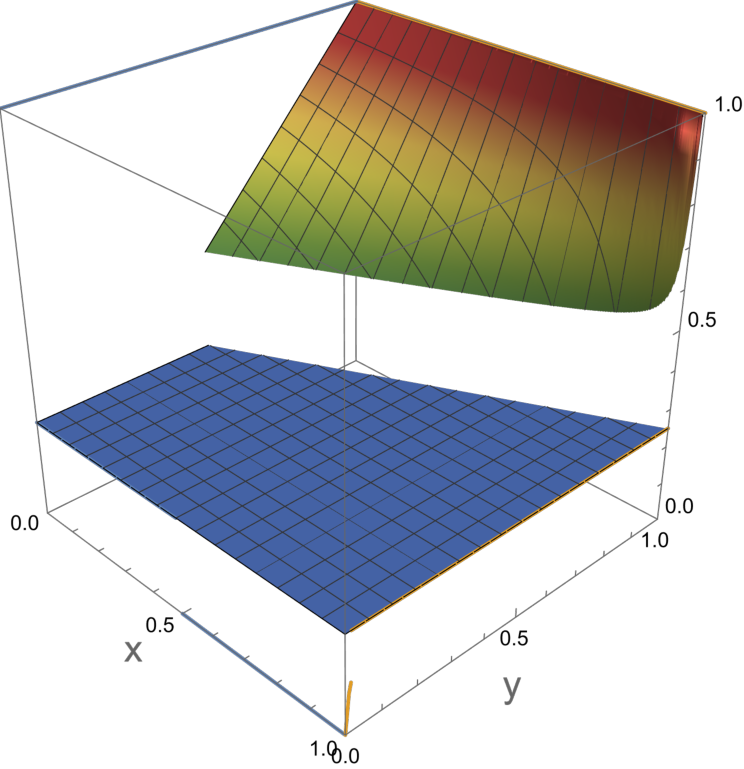
\includegraphics[width=0.9\linewidth]{Example3-1.pdf}
		\caption{$I_{\varphi_1,f_1,g_1}^{\TLK}$}	
	\end{subfigure}%
	\begin{subfigure}[t]{0.27\linewidth}\vspace{0pt}
		\centering
		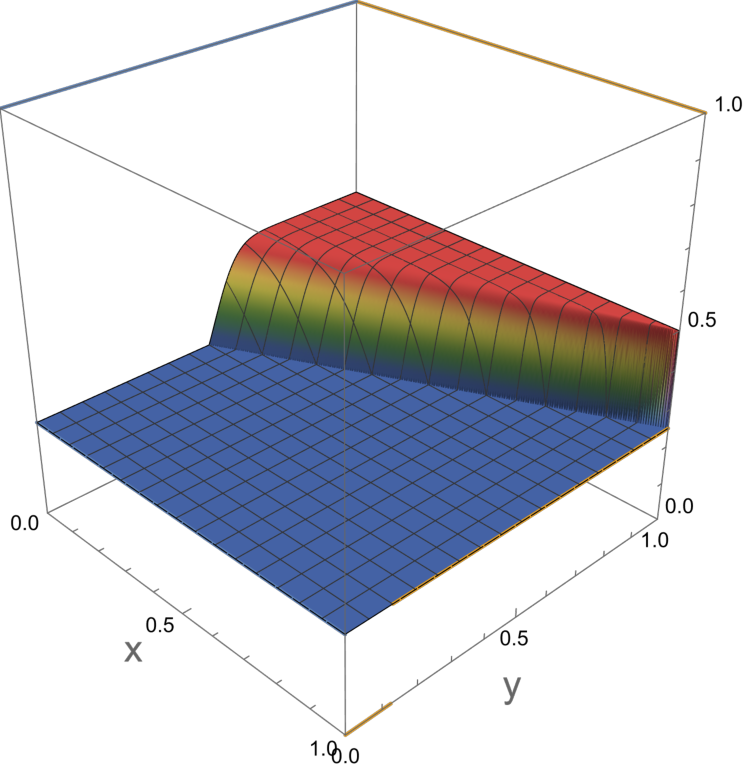
\includegraphics[width=0.9\linewidth]{Example3-2.pdf}
		\caption{$I_{\varphi_2,f_2,g_2}^{\TLK}$}
	\end{subfigure}%
	\begin{subfigure}[t]{0.27\linewidth}\vspace{0pt}
		\centering
		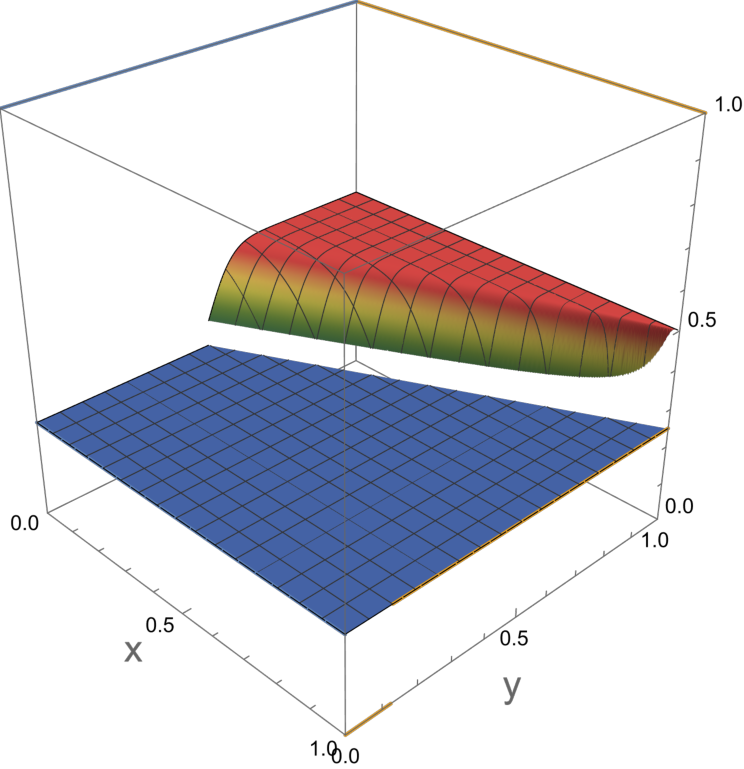
\includegraphics[width=0.91\linewidth]{Example3-3.pdf}
		\caption{$I_{\varphi_3,f_2,g_2}^{\TLK}$}		
	\end{subfigure}\\
	\begin{subfigure}[t]{0.27\linewidth}\vspace{0pt}
		\centering
		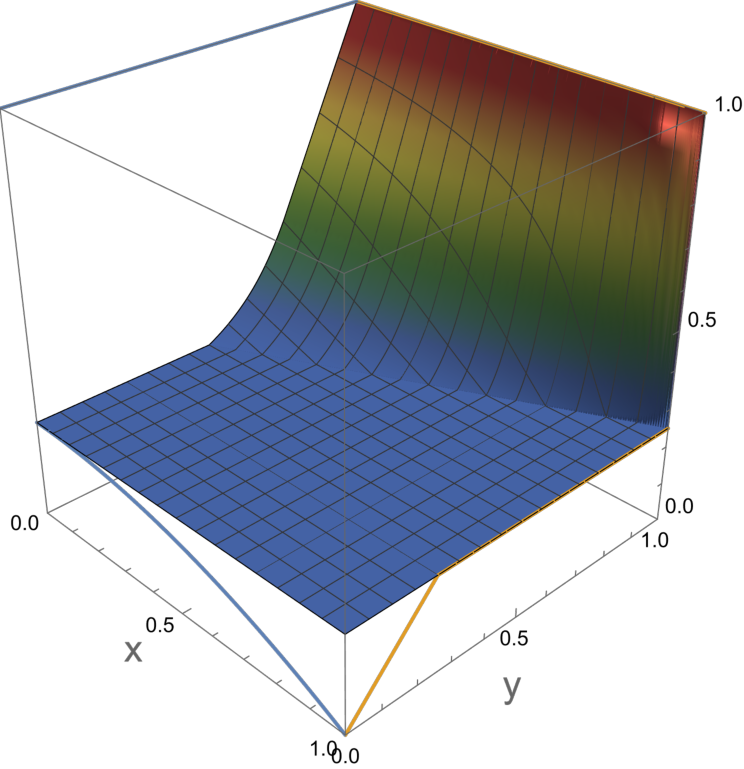
\includegraphics[width=0.9\linewidth]{Example3-4.pdf}
		\caption{$I_{\varphi_4,f_3,g_3}^{\TLK}$}	
	\end{subfigure}%
	\begin{subfigure}[t]{0.27\linewidth}\vspace{0pt}
		\centering
		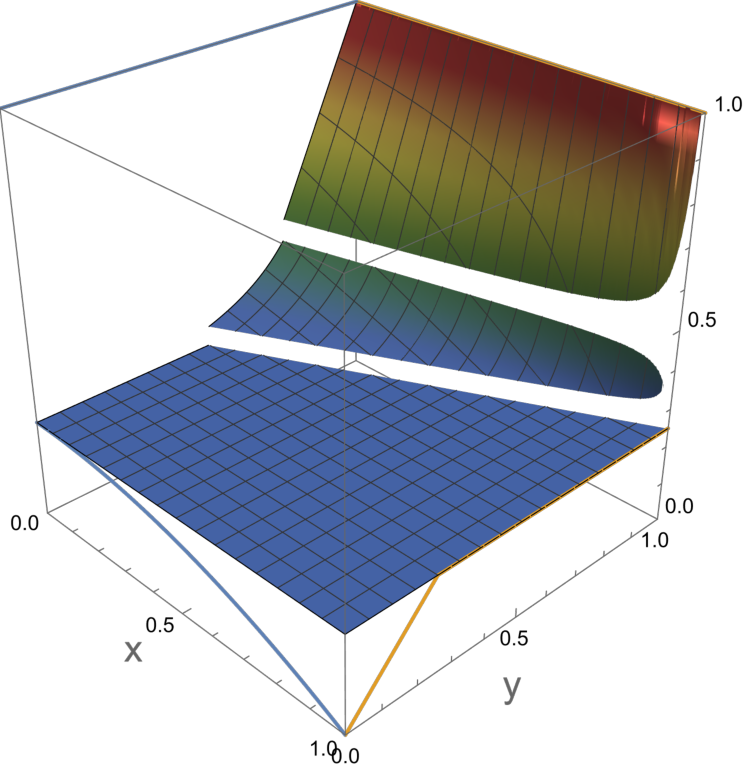
\includegraphics[width=0.9\linewidth]{Example3-5.pdf}
		\caption{$I_{\varphi_5,f_3,g_3}^{\TLK}$}
	\end{subfigure}
	\caption[Plot of five nilpotent $\TLK$-power invariant implications that satisfy \EP.]{Plots of nilpotent $\TLK$-power invariant implications that satisfy \EP considered in Example \ref{example:nilpotent:(EP)}.}\label{figure:nilpotent:(EP)}
\end{figure}
\end{example}

\begin{remark}\label{remark:strict:(NPe)}
	It is interesting to notice that, in contrast with the analogous situation in the strict case (see Remark \ref{remark:(NPe)}), in the nilpotent case none of the solutions of \EP satisfy \NPe. Indeed, if \IT is a nilpotent $T$-power invariant implication satisfying \NPe then by Proposition \ref{prop:nilpotent:(NPe)}, \IT is given by Equation (\ref{eq:CandidateRU}). Then, since $\frac{t(e)}{t(0)}<1$ the constant region of $\varphi$ does not include (0,1) and this function does not correspond to any of the situations of Lemma \ref{lemma:nilpotent:(EP)varphi} and then it does not satisfy \EP.
\end{remark}

% LAW OF IMPORTATION %
Consecutively, we study the law of importation with respect to some t-norm. It is well known that \LI implies \EP, so our starting point are the fuzzy implication functions described in Proposition \ref{prop:nilpotent:(EP)}. We have seen that the solutions of \EP are significantly different in the strict and nilpotent cases so, one would expect the same situation when studying the law of importation. However, the next result proves that a nilpotent $T$-power invariant implication \IT that satisfies \LI must be constant in $(0,1)^2$. Then, by Lemma \ref{lem:nilpotent:InvariantVarphiConstant} we know that \IT is invariant with respect to the positive powers of any continuous t-norm, in particular, it is a strict $T^*$-power invariant implication for any strict t-norm $T^*$. Thus, the results on the law of importation in the strict case from Section \ref{subsection:additional_propertiesStrictTpower} are also valid for the nilpotent case and we do not list them here.
\pagebreak

\begin{lemma}\label{lem:nilpotent:(LI)}
Let \IT be a nilpotent $T$-power invariant implication that satisfies \LI with respect to a t-norm $T^*$, then there exists a $k \in [0,1]$ such that $\varphi(w)=k$ for all $w \in (0,+\infty)$.
\end{lemma}

\begin{proof}
It is well known that if \IT satisfies \LI with respect to a t-norm $T^*$ then it also fulfills \EP. Thus, $\varphi$ has one of the structures in Lemma \ref{lemma:nilpotent:(EP)varphi} and, in particular, $\varphi$ is constant to 1 in $(0,+\infty)$ or there exist $k \in [0,1)$ and $\alpha \in \left [ \frac{t(0)}{t(k)},1\right)$ such that $\varphi(w)=k$ for all $w \in (0,\alpha|$ and $\Ima g \subseteq [0,k]$. For this second case, let us consider $(y,z) \in (0,1)^2$ with $\IT(y,z) \in (0,1)$. Then,
$$k \leq \IT(y,z)=\IT(T^*(1,y),z)=\IT(1,\IT(y,z)) = g(\IT(y,z)) \leq k,$$
and $\IT(y,z)=k$. If $\IT(y,z) \in \{0,1\}$ for all $(y,z) \in (0,1)^2$ then by Lemma \ref{lemma:nilpotent:(EP)varphi} either $\varphi(w)=0$ for all $w \in [0,+\infty)$ or $\varphi(w)=1$ for all $w \in (0,+\infty]$. Thus, every situation leads to a $\varphi$  which is constant in $(0,+\infty)$.
\end{proof}

% ITERATIVE BOOLEAN RULE  %

Next, we consider the iterative boolean law. In this case, we can prove that $\varphi$ cannot be strictly increasing and, any interval in which $\varphi$ is constant to some $k \in (0,1)$ can be extended to $(0,+\infty)$.

\begin{lemma}\label{lem:nilpotent:(IB)}
Let \IT be a nilpotent $T$-power invariant implication that satisfies \IB. Then, the following properties hold:
\begin{enumerate}[label=(\roman*)]
	\item $g(y)=y$ for all $y \in \Ima g \setminus \{0,1\}$.
	\item $\varphi$ is not strictly increasing.
	\item If there exists a constant $k \in (0,1)$ and an interval $(a,b)$ with $a,b \in [0,+\infty)$ and $a<b$ such that $\varphi(w)=k$ for all $w \in (a,b)$ then $\varphi(w)=k$ for all $w \in (0,+\infty)$.
\end{enumerate}
\end{lemma}

\begin{proof}
\begin{enumerate}[label=(\roman*)]
	\item Consider $z \in \Ima g \setminus \{0,1\}$ then there exists $y \in (0,1)$ such that $g(y)=z$ and
	$$z=g(y)=\IT(1,y)=\IT(1,\IT(1,y))=\IT(1,z)=g(z).$$
	\item Assume that $\varphi$ is strictly increasing, then
	$$\varphi(1)=\IT(x,x)=\IT(x,\IT(x,x)) =\IT(x,\varphi(1)) = \varphi \left(\frac{t(x)}{t \circ \varphi(1)}\right),$$
	and $t(x)=t \circ \varphi(1)$ for all $x \in (0,1)$. Contradiction with the fact that $t$ is the additive generator of a nilpotent t-norm.
	\item First of all, we prove that $\varphi(w)=k$ for all $w \in \left(0,\frac{t(0)}{t(k)}\right)$ distinguishing between two cases:
	\begin{itemize}
		\item If $a \geq 1$ we consider $x_0 \in (0,1)$ and $y_0 \in \left( t^{-1} \left(\frac{t(x_0)}{a}\right), t^{-1} \left(\frac{t(x_0)}{b}\right)\right)$. In this case,
		$$k = \varphi \left(\frac{t(x_0)}{t(y_0)}\right) = \IT(x_0,y_0) = \IT(x_0,\IT(x_0,y_0)) = \IT(x_0,k) = \varphi \left(\frac{t(x_0)}{t(k)}\right).$$
		Thus, $\varphi(w)=k$ for all $w \in \left(0,\frac{t(0)}{t(k)}\right)$.
		\item If $a < 1$ then there exists an $n_0 \in \NN$ with $\left( \frac{t(0)}{t(k)} \right)^{n_0-1}a<1$ and $\left( \frac{t(0)}{t(k)} \right)^{n_0}a \geq 1$. We prove by induction on $n \in \{1,\dots,n_0\}$ that $\varphi(w)=k$ for all $w \in \left(0,\left(\frac{t(0)}{t(k)}\right)^{n_0}a\right)$.
		\begin{itemize}
			\item If $n=1$ we consider $x_0 > t^{-1}(a t(0))$ and $y_0 \in \left( t^{-1} \left(\frac{t(x_0)}{a}\right), t^{-1} \left(\frac{t(x_0)}{b}\right)\right)$. Then,
			\begin{eqnarray*}
			k &=& \varphi \left(\frac{t(x_0)}{t(y_0)}\right) = \IT(x_0,y_0) = \IT(x_0,\IT(x_0,y_0))= \IT(x_0,k) \\
			&=& \varphi \left(\frac{t(x_0)}{t(k)}\right),
			\end{eqnarray*}
			and $\varphi(w)=k$ for all $w \in \left(0,\frac{t(0)}{t(k)}a\right)$.
			\item We assume that $\varphi(w)=k$ for all $w \in \left(0,\left(\frac{t(0)}{t(k)}\right)^{n-1}a\right)$. Let us choose $x_0 > t^{-1} \left(a \frac{t(0)^n}{t(k)^{n-1}}\right)$ and $y_0 < t^{-1} \left(\frac{t(x_0)}{a} \left(\frac{t(k)}{t(0)}\right)^{n-1}\right)$. Then,
			\begin{eqnarray*}
			k &=& \varphi \left(\frac{t(x_0)}{t(y_0)}\right) = \IT(x_0,y_0) = \IT(x_0,\IT(x_0,y_0))= \IT(x_0,k) \\
			&=& \varphi \left(\frac{t(x_0)}{t(k)}\right),
			\end{eqnarray*}
			and $\varphi(w)=k$ for all $w \in \left(0,\left(\frac{t(0)}{t(k)}\right)^n a\right)$.
		\end{itemize}
		Finally, let us consider $x_0 \in (0,1)$ and $y_0 < t^{-1} \left(\frac{t(x_0)t(k)^{n_0}}{at(0)^{n_0}}\right)$. Then,
		$$k = \varphi \left(\frac{t(x_0)}{t(y_0)}\right) = \IT(x_0,y_0) = \IT(x_0,\IT(x_0,y_0))= \IT(x_0,k) = \varphi \left(\frac{t(x_0)}{t(k)}\right),$$
		and  $\varphi(w)=k$ for al $w \in \left(0,\frac{t(0)}{t(k)}\right)$.			
	\end{itemize}
	On the other hand, assume that there exists a $w_0 \in \left[ \frac{t(0)}{t(k)},+\infty\right)$ with $\varphi(w_0)>k$. Then, $t \circ \varphi (w_0) < t(k) \Rightarrow \frac{t \circ \varphi(w_0)}{t(k)} < 1 \Rightarrow \frac{t \circ \varphi(w_0)t(0)}{t(k)}<t(0)$. Let us choose $x_0 \in \left(t^{-1} \left(\frac{t(0) t \circ \varphi(w_0)}{t(k)}\right),1\right)$, since  $\frac{t(x_0)}{t(0)}<1<\frac{t(0)}{t(k)} \leq w_0$ there exists a $y_0 \in (0,1)$ such that $\frac{t(x_0)}{t(y_0)}=w_0$. In this case,
	\begin{eqnarray*}
	\varphi(w_0) &=& \varphi\left(\frac{t(x_0)}{t(y_0)}\right) = \IT(x_0,y_0) = \IT(x_0,\IT(x_0,y_0)) =\IT(x_0,\varphi(w_0)) \\
	&=& \varphi \left(\frac{t(x_0)}{t \circ \varphi(w_0)}\right)=k,
	\end{eqnarray*}
	which is a contradiction. Then $\varphi$ is constant to $k$ in $(0,+\infty)$.
\end{enumerate}
\end{proof}

The next result characterizes the nilpotent $T$-power invariant implications that satisfy \IB.

\begin{proposition}\label{prop:nilpotent:(IB)}
Let \IT be a nilpotent $T$-power invariant implication. Then \IT satisfies \IB if and only if one of the following conditions hold:
\begin{enumerate}[label=(\roman*)]
	\item $\varphi(w)=0$ for all $w \in (0,+\infty)$ and $f(x)=g(y)=0$ for all $x,y \in (0,1)$.
	\item 						$$
	\varphi(w)
	=
	\left\{ \begin{array}{ll}
		0 &   \text{if }   w \in (0,b|, \\
		1 & \text{if } w \in (0,+\infty] \setminus (0,b|,
	\end{array}
	\right.
	$$
	where $b \in (0,1)$, $ \Ima f \subseteq \{0,1\}$, $f(x)=0$ for all $x \in (0,1)$ such that $\frac{t(x)}{t(0)} \in (0,b|$ and $g(y)=0$ for all $y \in (0,1)$.
	\item Let $k \in (0,1]$, then $\varphi(w)=k$ for all $w \in (0,+\infty)$, $\Ima f  \subseteq \{0,k\}$, $\Ima g \subseteq [0,k]$ and $g(y)=y$ for all $y \in \Ima g \setminus \{0,1\}$.
\end{enumerate}
\end{proposition}

\begin{proof}
\begin{itemize}
	\item[($\Rightarrow$)] By (ii)-Lemma \ref{lem:nilpotent:(IB)} we know that $\varphi$ is not strictly increasing, i.e., it is constant in some interval. We distinguish between four cases:
	\begin{enumerate}[label=\alph*)]
		\item $\varphi(w)=0$ for all $w \in (0,+\infty)$ then by Lemma \ref{lem:nilpot:monotonicity_condition:necessicity} we have that $f(x)=g(y)=0$ for all $x,y \in (0,1)$ and we are in Case (i).
		\item If there exists a $b \in (0,+\infty)$ such that $\varphi(w)=0$ if and only if $w \in (0,b|$, then by Lemma \ref{lem:nilpot:monotonicity_condition:necessicity}, $g(y)=0$ for all $y \in (0,1)$ and by Condition (\ref{eq:def:nilpot:TPowerInv:MonotonicityCond}) we get that $f(x)=0$ when $\frac{t(x)}{t(0)} \in (0,b|$ for all $x \in (0,1)$. Let us consider $\varphi(w_0) \in (0,1)$ with $w_0 \in (0,+\infty) \setminus (0,b|$, if we choose $x_0>t^{-1} (\min \{t(0),bt \circ \varphi(w_0)\})$ then $\frac{t(x_0)}{t(0)}< \frac{b t \circ \varphi(w_0)}{t(0)}<b$ and there exists a $y_0 \in (0,1)$ such that $\frac{t(x_0)}{t(y_0)}=w_0$. Thus,
		\begin{eqnarray*}
			\varphi(w_0)&=&\varphi \left(\frac{t(x_0)}{t(y_0)}\right) = \IT(x_0,y_0) = \IT(x_0,\IT(x_0,y_0)) = \IT(x_0,\varphi(w_0)) \\
			&=& \varphi \left(\frac{t(x_0)}{t \circ \varphi(w_0)}\right)=0,
		\end{eqnarray*}
		and we obtain a contradiction with the fact that \IT satisfies \IB. Then $\Ima \varphi \subseteq \{0,1\}$ and we are in Case (ii).
		\item If $\varphi(w)=k$ with $k \in (0,1)$ for all $w \in (a,b)$ with $a,b \in [0,+\infty)$ and $a<b$, by (iii)-Lemma \ref{lem:nilpotent:(IB)} we have that $\varphi(w)=k$ for all $w \in (0,+\infty)$.
		\item Consider the situation where there exists $a \in (0,+\infty)$ such that $\varphi(w)=1$ for all $w \in |a,+\infty]$. If $\varphi(w_0)=0$ for some $w_0 \in (0,a]$ we are in the same situation as in b), then we assume that $\varphi(w) \in (0,1]$ for all $w \in (0,+\infty]$. On the other hand, if $\varphi$ is constant to some $k \in (0,1)$ in some interval, by c) we would obtain a contradiction, then $\varphi$ must be strictly increasing when it is not constant to 1. Let us assume that there exists a $w_0 \in (0,a]$ with $\varphi(w_0) \in (0,1)$, then if we choose $x_0 > t^{-1}(\min \{t(0), w_0 t \circ \varphi(w_0)\})$ we have $\frac{t(x_0)}{t(0)} < \frac{w_0 t \circ \varphi(w_0)}{t(0)} < w_0$ and there exists $y_0 \in (0,1)$ such that $\frac{t(x_0)}{t(y_0)}=w_0$. Then,
		\begin{eqnarray*}
		\varphi(w_0) &=& \varphi \left(\frac{t(x_0)}{t(y_0)}\right) = \IT(x_0,y_0) = \IT(x_0,\IT(x_0,y_0)) \\
		&=& \IT(x_0,\varphi(w_0)) 
		= \varphi \left(\frac{t(x_0)}{t \circ \varphi(w_0)}\right).
		\end{eqnarray*}
		Since $\varphi$ is strictly increasing, we have $t(x_0)=w_0 t \circ \varphi(w_0)$. Contradiction with the fact that $x_0$ was selected to satisfy $t(x_0)<w_0t\circ \varphi(w_0)$. Then, $\varphi(w)=1$ for all $w \in (0,+\infty)$.	
	\end{enumerate}
	The points b) and c) correspond to situations where $\varphi(w)=k$ for all $w \in (0,+\infty)$ with $k \in (0,1]$. By Lemma \ref{lem:nilpot:monotonicity_condition:necessicity} we have $\Ima f \subseteq [0,k]$ and $\Ima g \subseteq [0,k]$ and by (i)-Lemma \ref{lem:nilpotent:(IB)} we know that $g(y)=y$ for all $y \in \Ima g \setminus \{0,1\}$. Let us assume that there exists an $x_0 \in (0,1)$ with $f(x_0) \in (0,k)$, then
	$$f(x_0) = \IT(x_0,0) = \IT(x_0,\IT(x_0,0)) = \IT(x_0,f(x_0))=k,$$
	which is a contradiction. Then, this situation corresponds to Case (iii).  
	\item[($\Leftarrow$)] Cases (i) and (iii) do not depend on the additive generator of the t-norm $T$, so these solutions were already considered in Proposition \ref{prop:strict:(IB)}. Then, we only check Case (ii). On the one hand,
	$$
	\IT(x,y)
	=
	\left\{ \begin{array}{ll}
		0 &   \text{if }   x=1 \text{ and } y \in (0,1), \\
		0 &   \text{if }   x,y \in (0,1) \text{ and } \frac{t(x)}{t(y)} \in (0,b|, \\
		f(x) &   \text{if }   x \in (0,1) \text{ and } y=0, \\
		1 & \text{otherwise}.
	\end{array}
	\right.
	$$
	On the other hand,
	\begin{eqnarray*}
		\IT(x,\IT(x,y))
		&=&
		\left\{ \begin{array}{ll}
			\IT(1,0) &   \text{if }   x=1 \text{ and } y \in (0,1), \\[1pt]
			\IT(x,0) &   \text{if }   x,y \in (0,1) \text{ and } \frac{t(x)}{t(y)} \in (0,b|, \\[3pt]
			\IT(x,f(x)) &   \text{if }   x \in (0,1) \text{ and } y=0, \\[3pt]
			\IT(x,1) & \text{otherwise},
		\end{array}
		\right. \\
		&=&
		\left\{ \begin{array}{ll}
			0 &   \text{if }   x=1 \text{ and } y \in (0,1), \\
			0 &   \text{if }   x,y \in (0,1) \text{ and } \frac{t(x)}{t(y)} \in (0,b|, \\
			\IT(x,0) &   \text{if }   x \in (0,1), y=0 \text{ and } f(x)=0, \\[3pt]
			\IT(x,1) &   \text{if }   x \in (0,1), y=0 \text{ and } f(x)=1, \\
			1 & \text{otherwise}, 
		\end{array} \right.  \\
		&=& \IT(x,y). 
	\end{eqnarray*}
	
\end{itemize}
\end{proof}

In this case, the solutions are very similar to the strict case (see Proposition \ref{prop:strict:(IB)}). However, notice that in Case (ii) the expression of the corresponding nilpotent $T$-power invariant depends on the generator $t$, so it is not the same situation of Case (i) in Proposition \ref{prop:strict:(IB)} and the strict and nilpotent cases are not equivalent.

Finally, we study the $T$-conditionality with respect to the same t-norm considered in the invariance property. For this property we obtain very different results than in the strict case (see Proposition \ref{prop:strict:(TC)}) since we obtain solutions that are not necessary $0$ whenever $x>y$. Indeed, a nilpotent $T$-power invariant implications satisfies \TC with respect to $T$ if and only if $\varphi$ and $f$ satisfy a certain inequality involving an additive generator of $T$.
\begin{proposition}\label{Nilpotent:(TC)}
	Let \IT be a nilpotent $T$-power invariant implication and $t$ an additive generator of~$T$. Then \IT satisfies  \TC with respect to $T$ if and only if $\varphi(w) \leq t^{-1} \left(t(0)(1-w)\right)$ for all $w \in [0,1)$, $f(x) \leq t^{-1}(t(0)-t(x))$ for all $x \in (0,1)$ and $g(y)=0$ for all $y \in (0,1)$.
\end{proposition}
\begin{proof}
	\begin{itemize}
		\item[$(\Rightarrow)$] Let \IT be a nilpotent $T$-power invariant implication that satisfies \TC with respect to $T$. Let us assume that there exists a $\tilde{w} \in (0,1)$ such that $\varphi(\tilde{w})>t^{-1}(t(0)(1-\tilde{w}))$, therefore, there exists a $\tilde{y} \in (0,1)$ such that $\varphi(\tilde{w})>t^{-1}(t(\tilde{y})(1-\tilde{w}))>t^{-1}(t(0)(1-\tilde{w}))$. Since $\left\{\frac{t(x)}{t(\tilde{y})} \mid x \in (0,1)\right\} = \left(0,\frac{t(0)}{t(\tilde{y})}\right)$ there exists an $\tilde{x} \in (\tilde{y},1)$ such that $\tilde{w}=\frac{t(\tilde{x})}{t(\tilde{y})}$. In this case,
		\begin{eqnarray*}
			\varphi(\tilde{w})>t^{-1}(t(\tilde{y})(1-\tilde{w})) & \Rightarrow &  \varphi\left(\frac{t(\tilde{x})}{t(\tilde{y})}\right)>t^{-1}\left(t\left(\tilde{y}\right)\left(1-\frac{t(\tilde{x})}{t(\tilde{y})}\right)\right)\\
			& \Rightarrow &  \varphi\left(\frac{t(\tilde{x})}{t(\tilde{y})}\right)>t^{-1}\left(t(\tilde{y})-t(\tilde{x})\right) \\
			& \Rightarrow &  t(\tilde{x}) + t\left(\varphi\left(\frac{t(\tilde{x})}{t(\tilde{y})}\right)\right)<t(\tilde{y})<t(0) \\
			& \Rightarrow &  t^{-1}\left(t(\tilde{x}) + t\left(\varphi\left(\frac{t(\tilde{x})}{t(\tilde{y})}\right)\right)\right) > \tilde{y} \\
			& \Rightarrow &  T(\tilde{x},I(\tilde{x},\tilde{y})) > \tilde{y},
		\end{eqnarray*}
		and we obtain a contradiction with the fact that \IT and $T$ satisfy \TC. On the other hand, let us assume that there exists an $\tilde{x} \in (0,1)$ such that $f(\tilde{x}) > t^{-1}(t(0)-t(\tilde{x}))$. Then, there exists a $\tilde{y} \in (0,1)$ such that $f(\tilde{x}) > t^{-1}(t(\tilde{y})-t(\tilde{x})) > t^{-1}(t(0)-t(\tilde{x}))$ and we have
		\begin{eqnarray*}
			f(\tilde{x}) > t^{-1}(t(\tilde{y})-t(\tilde{x}))  & \Rightarrow &  t(\tilde{x})+t(f(\tilde{x})) < t(\tilde{y})<t(0)\\
			& \Rightarrow &  t^{-1}\left(t(\tilde{x})+t(f(\tilde{x}))\right) > \tilde{y}\\
			& \Rightarrow &  T(\tilde{x},I(\tilde{x},0)) > \tilde{y} >0,
		\end{eqnarray*}
		and we obtain a contradiction with the fact that \IT and $T$ satisfy \TC. Finally, since $\displaystyle \lim_{w \to 0^+} \varphi(w) \leq \lim_{w \to 0^+} t^{-1} \left(t(0)(1-w)\right) = 0$ by Lemma \ref{lem:nilpot:monotonicity_condition:necessicity} we obtain that $g(y)=0$ for all $ y \in (0,1)$.
		\item[$(\Leftarrow)$] Let $x,y \in [0,1]$ with $x>y$. We distinguish between different cases:
		\begin{itemize}
			\item If $x=1$ and $y \in [0,1)$ then
			$$T(x,I(x,y))=T(1,I(1,y))=I(1,y)=\left\{ \begin{array}{ll}
				g(y) &   \text{if }   y \in (0,1), \\
				0 &  \text{if }   y=0,
			\end{array}
			\right.
			=0 \leq y.$$
			\item If $y=0$ and $x \in (0,1)$ then
			\begin{eqnarray*}
				I(x,0)=f(x) \leq t^{-1}(t(0)-t(x)) & \Rightarrow & t(x)+t(I(x,0)) \geq t(0)\\
				&\Rightarrow& t^{(-1)}(t(x)+t(I(x,0)))=0\\
				&\Rightarrow& T(x,I(x,0))=0=y.
			\end{eqnarray*}
			\item If $0<y<x<1$ then
			$$\varphi \left(\frac{t(x)}{t(y)}\right) \leq t^{-1}\left(t(0)\left(1-\frac{t(x)}{t(y)}\right)\right) \leq t^{-1}\left(t(y)\left(1-\frac{t(x)}{t(y)}\right)\right) = t^{-1}(t(y)-t(x)),$$
			$$t(x) + t \left(\varphi \left(\frac{t(x)}{t(y)}\right)\right) \geq t(y),$$
			and we distinguish between two cases.
			\begin{itemize}
				\item If $t(x) + t \left(\varphi \left(\frac{t(x)}{t(y)}\right)\right) \geq t(0)$ then
				$$T(x,I(x,y))= t^{(-1)}\left(t(x) + t \left(\varphi \left(\frac{t(x)}{t(y)}\right)\right)\right) = 0 \leq y.$$
				\item $t(x) + t \left(\varphi \left(\frac{t(x)}{t(y)}\right)\right) < t(0)$ then 
				$$T(x,I(x,y))=t^{-1}\left(t(x) + t \left(\varphi \left(\frac{t(x)}{t(y)}\right)\right)\right) \leq y.$$
			\end{itemize}
		\end{itemize}
	\end{itemize}
\end{proof}
Proposition \ref{Nilpotent:(TC)} discloses an important breakthrough. It is known that the $T$-conditionality is recommended for doing any inference with the generalized modus ponens when a fuzzy implication function is used as the generalization of the classical conditional to fuzzy logic. Therefore, it is a property which is required for many applications. Besides, we have already motivated the importance of the $T$-power invariance when fuzzy hedges modeled by powers of continuous t-norms are used. Proposition \ref{Nilpotent:(TC)} ensures the existence of many fuzzy implication functions satisfying \PIT and \TC with respect to a nilpotent t-norm $T$. From this fact, we can affirm that this family is very appealing for many practical applications. Not only that, the conditions in Proposition \ref{Nilpotent:(TC)} are general enough to allow some flexibility in the structure of the operator. Indeed, for instance if we consider $\varphi(w)= \alpha t^{-1}(t(0)(1-w))$ for all $w \in [0,1)$ with $\alpha \in (0,1)$ we have the freedom of choosing the values of the function $\varphi$ in  $w \in [1,+\infty]$ (as long as we respect the conditions in Definition \ref{def:nilpot:TPowerInv}). For instance, in Example \ref{example:ITLKalpha} we have considered $\varphi(w)=\frac{(1+\alpha)w+\alpha-1}{(1+\alpha)w-\alpha+1}$ for all  $w \in [1,+\infty]$ to define a family of fuzzy implication functions that is a particular case of those described in Proposition \ref{Nilpotent:(TC)}. It is curious how the invariance property together with other well-known properties like \NP or \LI is so strong that imposes that the corresponding nilpotent $T$-power invariant implication must be constant in $(0,1)^2$ and with other properties like \TC or \EP is flexible enough to allow us to select arbitrarily the expression of the operator in a subregion of $[0,1]^2$.
\begin{example}\label{example:ITLKalpha}
	Let $T$ be a nilpotent t-norm and $t$ an additive generator of $T$. Let us consider $\alpha \in (0,1]$ and $\varphi:[0,+\infty] \to [0,1]$, $g:(0,1) \to [0,1]$, $f: (0,1) \to [0,1]$ given by
	$$f(x)=g(y)=0, \quad \text{ for all } x,y \in (0,1),$$
	$$\varphi(w) 
	=
	\left\{ \begin{array}{ll}
		\alpha t^{-1}(t(0)(1-w)) &   \text{if }   w \in [0,1), \\
		\frac{(1+\alpha)w+\alpha-1}{(1+\alpha)w-\alpha+1} & \text{if } w \in [1,+\infty].
	\end{array}
	\right.
	$$
	Then, according to Proposition \ref{Nilpotent:(TC)} the corresponding nilpotent $T$-power invariant implication satisfies \TC with respect to $T$ for all $\alpha \in (0,1]$. Let us denote this family of functions as $I_{\alpha}^T : [0,1]^2 \to [0,1]$, their expression is
	\begin{equation}\label{eq:Family(TC)(IT)}
		I_{\alpha}^T(x,y) =\left\{ \begin{array}{ll}
			0 &   \text{if }   (x \in (0,1] \text{ and } y=0) \text{ or } (x = 1 \text{ and } y\in (0,1)), \\
			\alpha t^{-1}\left(t(0) \left(1-\frac{t(x)}{t(y)}\right)\right) & \text{if } 0<y<x<1, \\
			\frac{(1+\alpha)t(x)-(1-\alpha)t(y)}{(1+\alpha)t(x)+(1-\alpha)t(y)} & \text{if } 0<x\leq y<1, \\
			1 & \text{if } (x=0 \text{ and } y \in [0,1]) \text{ or } (x \in (0,1] \text{ and } y=1),
		\end{array}
		\right.
	\end{equation}
	for all $\alpha \in (0,1]$. In Figure \ref{fig:IalphaT} we can find a sketch of the structure of this subfamily of nilpotent $T$-power invariant implications. In particular, if we select $\alpha=1$ we have a family that also satisfies \IP and \OP  (see Proposition \ref{prop:nilpotent:(OP)n(IP)}).
	\begin{figure}[htp!]
		\centering
		\begin{tikzpicture}[xscale=5.5, yscale=5.5]
			\draw (0,0) rectangle (1,1);
			\node [above right] at (1,1) {\small 1} ;
			\node [below right] at (1,0) {\small 0};
			\node [below left] at (0,0) {\small 1};
			\node [above left] at (0,1) {\small 1};
			\node [above] at (0.5,1) {\small 1};
			\node [left] at (0,0.5) {\small 1};
			\node [above,rotate=45] at (0.5,0.5) {\small $\alpha$};
			\draw (0,0) -- (1,1);
			\node at (0.35,0.85) {\small $\frac{(1+\alpha)t(x)-(1-\alpha)t(y)}{(1+\alpha)t(x)+(1-\alpha)t(y)}$};
			\node at (0.6,0.15) {\small $\alpha t^{-1}\left(t(0) \left(1-\frac{t(x)}{t(y)}\right)\right)$};
			\node [below] at (0.5,0) {\small $0$};
			\node [right] at (1,0.5) {\small $0$};
		\end{tikzpicture}
		\caption{Schema of the structure of $I_{\alpha}^T$.}\label{fig:IalphaT}
	\end{figure}
	\begin{figure}[t!]
		\centering
		\begin{subfigure}[t]{0.35\linewidth}\vspace{0pt}
			\centering
			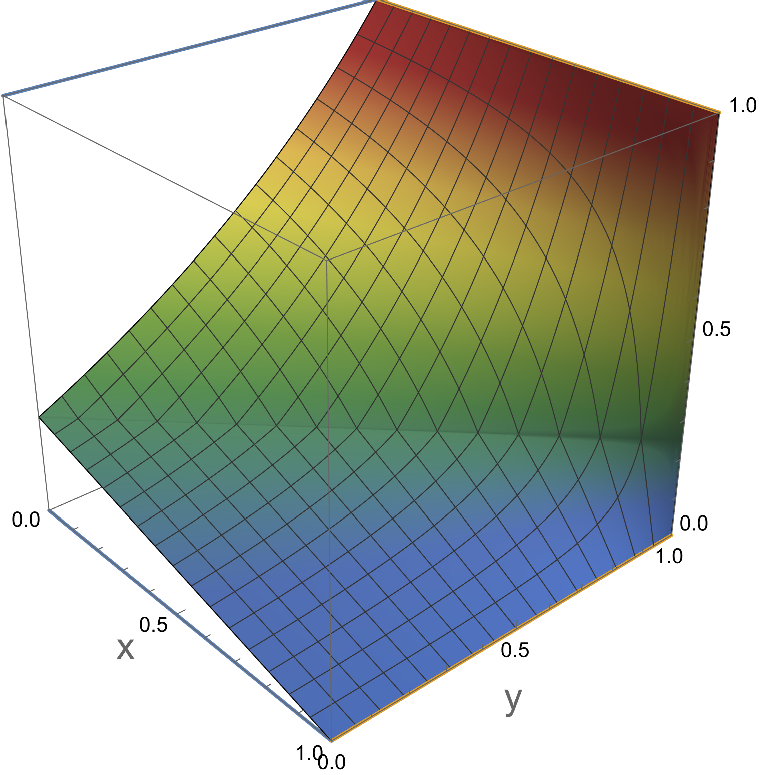
\includegraphics[width=0.9\linewidth]{ITalpha0.25.pdf}
			\caption{$I_{\alpha=0.25}^{\TLK}$}	
		\end{subfigure}%
		\begin{subfigure}[t]{0.35\linewidth}\vspace{0pt}
			\centering
			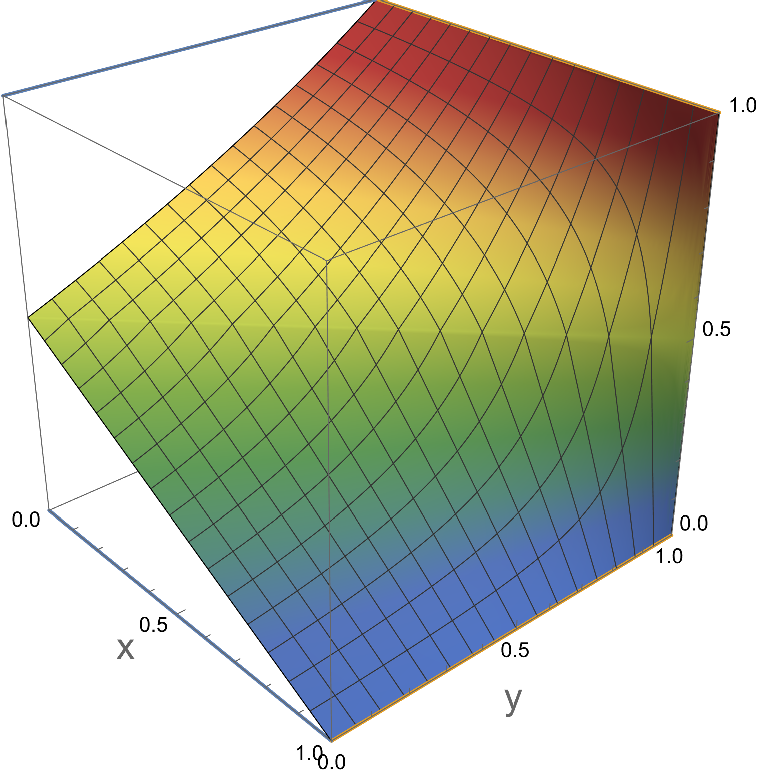
\includegraphics[width=0.9\linewidth]{ITalpha0.5.pdf}
			\caption{$I_{\alpha=0.5}^{\TLK}$}
		\end{subfigure}\\ \vspace{0.5cm}
		\begin{subfigure}[t]{0.35\linewidth}\vspace{0pt}
			\centering
			\includegraphics[width=0.91\linewidth]{ITalpha0.75.pdf}
			\caption{$I_{\alpha=0.75}^{\TLK}$}		
		\end{subfigure}%
		\begin{subfigure}[t]{0.35\linewidth}\vspace{0pt}
			\centering
			\includegraphics[width=0.9\linewidth]{ITalpha1.pdf}
			\caption{$I_{\alpha=1}^{\TLK}$}	
		\end{subfigure}
		\caption{Plot of the fuzzy implication function $I^T_{\alpha}$ where $T=\TLK$ for different values of the parameter $\alpha$.}\label{figure:ITLKalpha}
	\end{figure}
\end{example}
\begin{remark}
	The reader might have noticed that, unlike the case of the study of \LI, for \TC we have not considered the problem for a t-norm $T^*$ that might be different from the one used when imposing \PIT. We have decided not to study this case because of the complexity attached. It is rather straightforward to notice that \TC is more complex to study than \LI in this case because the first one is an inequality. However, some results in the particular case of $T$-power based implications can be found in \cite{Li2022,Peng2022}.
\end{remark}

\subsection{Summary}
To end this section we provide a summary in Table  \ref{table:summaryTpowerinvadditionalprop} of all the additional properties studied for the family of $T$-power invariant implication where $T$ is a continuous Archimedean t-norm and also of $T$-power based implications as a particular case. In this table, we can compare two perspectives: to study a family that satisfies a certain property and to study a family characterized by the fact that they fulfill a certain property. It is intuitive to think that the second perspective is much more stronger and provides more information. Indeed, in this chapter we have empirically proved this fact. In Table  \ref{table:summaryTpowerinvadditionalprop} we can see that although the power based implications satisfy the invariance property, they do not satisfy many of the other additional properties of fuzzy implication functions. On the other hand, studying the families characterized by the fact that they fulfill \PIT with respect to a certain Archimedean t-norm we have proved that there is always a choice satisfying also another additional property (except the continuity). Furthermore, as argued along the section, in this study we have obtain many interesting fuzzy implication functions which behave very differently from power-based implications. \enlargethispage{12pt}
\begin{table}[!t]
	\begin{adjustbox}{max width=\textwidth}
	\begin{tabular}{c|cc|cc|}
		\cline{2-5}
		\multicolumn{1}{l|}{}                  & \multicolumn{2}{l|}{\bf $T$-power based implications} & \multicolumn{2}{l|}{\bf $T$-power invariant implications} \\ \cline{2-5} 
		& \multicolumn{1}{c|}{\bf $T$ strict}   & \bf $T$ nilpotent   & \multicolumn{1}{c|}{\bf $T$ strict}     & \bf $T$ nilpotent     \\ \hline
		\multicolumn{1}{|c|}{\bf Continuity}       & \multicolumn{1}{c|}{\xmark}           &   \multicolumn{1}{c|}{\xmark}            & \multicolumn{1}{c|}{\begin{tabular}[c]{@{}c@{}c@{}}\xmark\\ Proposition \ref{prop:strict:continuity} \\ Corollary \ref{cor:strict:discontinuous} \end{tabular}}            &        \begin{tabular}[c]{@{}c@{}c@{}}\xmark\\ Proposition \ref{prop:nilpotent:continuity} \\ Corollary \ref{cor:nilpotent:discontinuous} \end{tabular}         \\ \hline
		\multicolumn{1}{|c|}{\bf Natural Negation}   & \multicolumn{1}{c|}{\NDOne}           &      \multicolumn{1}{c|}{$N_{I^T}(x)=\frac{t(x)}{t(0)}$}         & \multicolumn{1}{c|}{Corollary \ref{cor:strict:natural_negation}}             &        \multicolumn{1}{c|}{Corollary \ref{cor:nilpotent:natural_negation}}          \\ \hline
		\multicolumn{1}{|c|}{\bf Trivial 1-region} & \multicolumn{1}{c|}{\xmark}            &  \multicolumn{1}{c|}{\xmark}              & \multicolumn{1}{c|}{Proposition \ref{prop:strict:1-region}}             &   \multicolumn{1}{c|}{Proposition \ref{prop:nilpotent:1-region}}               \\ \hline
		\multicolumn{1}{|c|}{\CB}             & \multicolumn{1}{c|}{\xmark}            &    \multicolumn{1}{c|}{\xmark}            & \multicolumn{1}{c|}{\begin{tabular}[c]{@{}c@{}} Proposition \ref{prop:strict:(CB)} \\ Constant in $(0,1)^2$ \end{tabular}}            &       \multicolumn{1}{c|}{\begin{tabular}[c]{@{}c@{}} Proposition \ref{prop:nilpot:(CB)} \\ Constant in $(0,1)^2$ \end{tabular}}          \\ \hline
		\multicolumn{1}{|c|}{\NP}             & \multicolumn{1}{c|}{\xmark}            &    \multicolumn{1}{c|}{\xmark}            & \multicolumn{1}{c|}{\begin{tabular}[c]{@{}c@{}} Proposition \ref{prop:strict:(NP)} \\ Constant in $(0,1)^2$ \end{tabular}}            &       \multicolumn{1}{c|}{\begin{tabular}[c]{@{}c@{}} Proposition \ref{prop:nilpotent:(NP)} \\ Constant in $(0,1)^2$ \end{tabular}}           \\ \hline
		\multicolumn{1}{|c|}{\NPe}            & \multicolumn{1}{c|}{\xmark}           &     \multicolumn{1}{c|}{\xmark}           & \multicolumn{1}{c|}{Proposition \ref{prop:strict:(NPe)}}             &     \multicolumn{1}{c|}{Proposition \ref{prop:nilpotent:(NPe)}}             \\ \hline
		\multicolumn{1}{|c|}{\IP}             & \multicolumn{1}{c|}{\cmark}            &       \multicolumn{1}{c|}{\cmark}         & \multicolumn{1}{c|}{Proposition \ref{prop:strict:(IP)n(OP)}}             &      \multicolumn{1}{c|}{Proposition \ref{prop:nilpotent:(OP)n(IP)}}            \\ \hline
		\multicolumn{1}{|c|}{\OP}             & \multicolumn{1}{c|}{\cmark}           &    \multicolumn{1}{c|}{\cmark}            & \multicolumn{1}{c|}{Proposition \ref{prop:strict:(IP)n(OP)}}             &     \multicolumn{1}{c|}{Proposition \ref{prop:nilpotent:(OP)n(IP)}}             \\ \hline
		\multicolumn{1}{|c|}{\EP}             & \multicolumn{1}{c|}{\xmark}            &     \multicolumn{1}{c|}{\xmark}           & \multicolumn{1}{c|}{Proposition \ref{prop:strict:(EP)}}             &      \multicolumn{1}{c|}{Proposition \ref{prop:nilpotent:(EP)}}           \\ \hline
		\multicolumn{1}{|c|}{\bf \LI with $T^*$}             & \multicolumn{1}{c|}{\xmark}           &        \multicolumn{1}{c|}{\xmark}        & \multicolumn{1}{c|}{\begin{tabular}[c]{@{}c@{}} Proposition \ref{prop:strict:(LI)} \\ Constant in $(0,1)^2$ \end{tabular}}             &     \multicolumn{1}{c|}{\begin{tabular}[c]{@{}c@{}c@{}} Lemma \ref{lem:nilpotent:(LI)} \\ Proposition \ref{prop:strict:(LI)} \\ Constant in $(0,1)^2$ \end{tabular}}             \\ \hline
		\multicolumn{1}{|c|}{\bf (IB)}             &\multicolumn{1}{c|}{\xmark}            & \multicolumn{1}{c|}{\xmark}               & \multicolumn{1}{c|}{Proposition \ref{prop:strict:(IB)}}             &          \multicolumn{1}{c|}{Proposition \ref{prop:nilpotent:(IB)}}         \\ \hline
		\multicolumn{1}{|c|}{\bf \TC with $T$}      & \multicolumn{1}{c|}{\xmark}           &  \multicolumn{1}{c|}{\cite[Theorem 3.2]{Peng2022}}             & \multicolumn{1}{c|}{Proposition \ref{prop:strict:(TC)}}             &       \multicolumn{1}{c|}{Proposition \ref{Nilpotent:(TC)}}            \\ \hline
	\end{tabular}
	\end{adjustbox}
\caption[Summary of the properties fulfilled by $T$-power based implications and by $T$-power invariant implications where $T$ is a continuous Archimedean t-norm.]{Summary of the properties fulfilled by $T$-power based implications and by $T$-power invariant implications where $T$ is a continuous Archimedean t-norm. The results involving $T$-power based implications are either available in \cite{Massanet2017} or they have been deduced from the results of this section.}\label{table:summaryTpowerinvadditionalprop}
\end{table}
\section{Intersections}\label{section:intersectionsTpower}

In this section, we investigate the intersections between the families of strict and nilpotent $T$-power invariant implications and ten of the main families of fuzzy implication functions. This step is very important when studying a new family of fuzzy implication functions since it proves that the newly introduced family is significantly different from other  families in the literature. Moreover, in our particular case, this study has an added value, since studying the intersection between the family of strict/nilpotent $T$-power invariant implications and another family is equivalent to characterize all the fuzzy implication functions of this family which are invariant with respect to $T$-powers of a certain strict/nilpotent t-norm.

First of all, we study the intersection between the studied families, i.e., strict and nilpotent $T$-power invariant implications. In Lemma \ref{lem:nilpotent:InvariantVarphiConstant} we have already proved that if $\varphi$ is constant, the dependence on the generator disappears, and a nilpotent $T$-power invariant implication is, in fact, invariant with respect to the positive powers of any continuous t-norm, so it is also a strict $T^*$-power invariant implication for any strict t-norm $T^*$. However, the following result completely characterizes the intersection between the two families, that will be denoted by:
\begin{eqnarray*}
	\mathbb{I}^{\infty}_{Inv} &~-~& \text{the family of all fuzzy implication functions which are invariant} \\
	&~~~& \text{with respect to the positive powers of some strict t-norm}; \\
	\mathbb{I}^{\aleph}_{Inv} &~-~& \text{the family of all fuzzy implication functions which are invariant} \\
	&~~~& \text{with respect to the positive powers of some nilpotent t-norm}.
\end{eqnarray*}

\begin{proposition}\label{prop:InterStrictNilpot}
	Let $I:[0,1]^2 \to [0,1]$ be a binary function. Then $I \in  \mathbb{I}^{\infty}_{Inv} \cap \mathbb{I}^{\aleph}_{Inv}$ if and only if there exist three constants $0 \leq k_1 \leq k_2 \leq k_3 \leq 1$, a decreasing function $f:(0,1) \to [0,k_1]$ and an increasing function $g:(0,1) \to [0,k_1]$ such that
	\begin{equation*}
		I(x,y) =\left\{ \begin{array}{ll}
			0 & \text{if } x=1 \text{ and } y=0,\\
			f(x) &   \text{if }   x \in (0,1) \text{ and } y=0, \\
			g(y) &  \text{if }  x = 1 \text{ and } y\in (0,1), \\
			k_1 &  \text{if } x,y \in (0,1) \text{ and } x>y, \\
			k_2 &  \text{if } x,y \in (0,1) \text{ and } x=y, \\
			k_3 &  \text{if } x,y \in (0,1) \text{ and } x<y, \\
			1 & \text{otherwise.}
		\end{array}
		\right.
	\end{equation*}
\end{proposition}
\begin{proof}
	Let $I \in  \mathbb{I}^{\infty}_{Inv} \cap \mathbb{I}^{\aleph}_{Inv}$, then there exists $t_1$ an additive generator of a strict t-norm $T_1$, $t_2$ an additive generator of a nilpotent t-norm $T_2$ and $\varphi_1: [0,+\infty] \to [0,1]$, $\varphi_2: [0,+\infty] \to [0,1]$ two increasing functions with $\varphi_1(0)=\varphi_2(0)=0$ and $\varphi_1(+\infty)=\varphi_2(+\infty)=1$ such that
	$$\varphi_1 \left(\frac{t_1(x)}{t_1(y)}\right) = I(x,y) = \varphi_2 \left(\frac{t_2(x)}{t_2(y)}\right), \quad \text{for all } x,y \in (0,1).$$
	It is clear that $\varphi_1(1)=\varphi_2(1)$. Let $y_0 \in (0,1)$, we have
	$$\varphi_1(1^-)=\lim_{w \to 1^{-}} \varphi_1(w)=\lim_{x \to y_0^+} \varphi_1 \left(\frac{t_1(x)}{t_1(y_0)}\right)=\lim_{x \to y_0^+} \varphi_2 \left(\frac{t_2(x)}{t_2(y_0)}\right) = \lim_{w \to 1^{-}} \varphi_2(w)=\varphi_2(1^-),$$
	$$\varphi_1(1^+)=\lim_{w \to 1^{+}} \varphi_1(w)= \lim_{x \to y_0^-} \varphi_1 \left(\frac{t_1(x)}{t_1(y_0)}\right)=\lim_{x \to y_0^-} \varphi_2 \left(\frac{t_2(x)}{t_2(y_0)}\right) =\lim_{w \to 1^{+}} \varphi_2(w)= \varphi_2(1^+).$$
	Now, we distinguish between two cases:
	\begin{itemize}
		\item If $w \in (1,+\infty)$, by the monotonicity of $\varphi_1$ we have $\varphi_1(w) \geq \varphi_1(1^+) = \varphi_2(1^+)$. For $y^* \in (0,1)$ and $x^* = t_1^{-1}(wt_1(y^*))$ we have
		$$\varphi_1(w)=\varphi_1 \left(\frac{t_1(x^*)}{t_1(y^*)}\right)=\varphi_2 \left(\frac{t_2(x^*)}{t_2(y^*)}\right) \leq \varphi_2 \left(\frac{t_2(0)}{t_2(y^*)}\right),$$
		$$\varphi_1(w) \leq \lim_{y^* \to 0^+} \varphi_2 \left(\frac{t_2(0)}{t_2(y^*)}\right) = \varphi_2(1^+)=\varphi_1(1^+), $$
		and then $\varphi_1(w) = \varphi_1(1^+)$ for all $w \in (1,+\infty)$.
		\item If $w \in (0,1)$, by the monotonicity of $\varphi_1$ we have $\varphi_1(w) \leq \varphi_1(1^-) = \varphi_2(1^-)$. For $x^* \in (0,1)$  and $y^*=t_1^{-1}\left(\frac{t_1(x^*)}{w}\right)$ we have
		$$\varphi_1(w) = \varphi_1 \left(\frac{t_1(x^*)}{t_1(y^*)}\right)= \varphi_2 \left(\frac{t_2(x^*)}{t_2(y^*)}\right) \geq \varphi_2 \left(\frac{t_2(x^*)}{t_2(0)}\right),$$
		$$\varphi_1(w) \geq \lim_{x^* \to 0^+} \varphi_2 \left(\frac{t_2(x^*)}{t_2(0)}\right) = \varphi_2(1^-)=\varphi_1(1^-),$$
		and then $\varphi_1(w)= \varphi_2(1^-) = \varphi_1(1^-)$ for all $w \in (0,1)$.
	\end{itemize}
	Thus, considering $k_1= \varphi_1(1^-)$, $k_2 = \varphi_1(1)=k_2$ and $\varphi_1(1^+)=k_3$, the result follows  by the definition of strict and nilpotent invariant implications.
\end{proof}

%\subsection{Intersections between strict or nilpotent $T$-power invariant implications and other families}\label{subsec:IntStrictOthers}

Now, let us highlight five fuzzy implication functions, which are either strict or nilpotent $T$-power invariant implications:

$$
\ILT(x,y)
=
\left\{ \begin{array}{ll}
	1 &   \text{if }   x=0 \text{ or } y=1, \\
	0 & \text{otherwise,}
\end{array}
\right. \quad
\IWB(x,y) =\left\{ \begin{array}{ll}
	y &  \text{if }  x = 1 \text{ and } y\in [0,1], \\
	1 &  \text{otherwise,}
\end{array}
\right.
$$
$$
I_{Inv}^{f}(x,y)
=
\left\{ \begin{array}{ll}
	f(x) &   \text{if }   x \in (0,1) \text{ and } y=0, \\
	y &   \text{if }   x=1 \text{ and } y \in [0,1), \\
	1 & \text{otherwise,}
\end{array}
\right.
$$
$$
I_{Inv}^{g}(x,y)
=
\left\{ \begin{array}{ll}
	0 &   \text{if }   x=1 \text{ and } y=0, \\
	g(y) &   \text{if }   x=1 \text{ and } y \in(0,1), \\
	1 & \text{otherwise,}
\end{array}
\right.
$$
$$
I_{Inv}^{t,C}(x,y)
=
\left\{ \begin{array}{ll}
	0 &   \text{if }   (x \in (0,1] \text{ and } y=0) \text{ or } (x=1 \text{ and } y \in (0,1)), \\
	t^{-1}\left(\frac{Ct(y)}{t(x)}\right) & \text{otherwise},
\end{array}
\right.
$$
where $f:(0,1) \to [0,1]$ is a decreasing function with $\Ima f \subseteq (0,1]$, $C \in (0,+\infty)$, $g:(0,1) \to [0,1]$ is an increasing function with $\Ran g \subseteq \{0,1\}$ and $t$ is an additive generator of a strict t-norm. By Proposition \ref{prop:InterStrictNilpot} it is clear that $I_{\text{Lt}}, I_{\text{WB}}, I_{Inv}^{f}, I_{Inv}^{g} \in \mathbb{I}^{\infty}_{Inv} \cap \mathbb{I}^{\aleph}_{Inv}$ and by Proposition \ref{prop:strict:(EP)}, $I_{Inv}^{t,C} \in \mathbb{I}^{\infty}_{Inv}$ and it satisfies \EP.

Next, we consider seven of the most recurring families of fuzzy implication functions:
\begin{eqnarray*}
	\mathbb{I}_{\mathbb{S},\mathbb{N}} &~-~& \text{the family of all $(S,N)$-implications};\\
	\mathbb{I}_{\mathbb{T}} &~-~& \text{the family of all $R$-implications};\\
	\mathbb{I}_{\mathbb{QL}} &~-~& \text{the family of all $QL$-implications};\\
	\mathbb{I}_{\mathbb{D}} &~-~& \text{the family of all $D$-implications};\\
	\mathbb{I}_{\mathbb{F}} &~-~& \text{the family of all $f$-generated implications};\\
	\mathbb{I}_{\mathbb{G}} &~-~& \text{the family of all $g$-generated implications};\\
	\mathbb{I}_{\mathbb{H}} &~-~& \text{the family of all $h$-generated implications}.
\end{eqnarray*}

All the above families have in common that they satisfy the left neutrality principle. In this sense, in \cite{Massanet2017} it was pointed out that $T$-power based implications do not satisfy \NP and then they have empty intersection with all these families. However, thanks to Propositions \ref{prop:strict:(NP)} and \ref{prop:nilpotent:(NP)} we know that there are choices for $f$, $g$ and $\varphi$ such that the corresponding strict or nilpotent $T$-power invariant implication satisfies \NP. Therefore, it is to be expected that the families of strict and nilpotent $T$-power invariant implications will have non-empty intersection with some of these families.  Indeed, the following result provides the complete characterization of the intersections of interest and shows that strict and nilpotent $T$-power invariant implications have non-empty intersection with $(S,N)$, $R$, $QL$ and $D$-implications. However, we know by Propositions \ref{prop:strict:(NP)} and \ref{prop:nilpotent:(NP)} that all strict and nilpotent $T$-power invariant fuzzy implication functions that satisfy \NP are constant to 1 in $(0,1)^2$, so only fuzzy implication functions which are constant to 1 in $(0,1)^2$ belong to the intersection. Moreover, by Proposition \ref{prop:InterStrictNilpot} we know that any nilpotent $T$-power invariant implication which is constant in $(0,1)^2$ is also a strict $T$-power invariant implication, so the study of the intersection is equivalent in the two cases.

\begin{proposition}\label{prop:intersections1}
	The following equalities are true:
	\begin{enumerate}[label=(\roman*)]
		\item $\mathbb{I}^{\infty}_{Inv} \cap \mathbb{I}_{\mathbb{T}} = \{I_{\textbf{WB}}\} = \mathbb{I}^{\aleph}_{Inv} \cap \mathbb{I}_{\mathbb{T}}.$
		\item $\mathbb{I}^{\infty}_{Inv} \cap \mathbb{I}_{\mathbb{S},\mathbb{N}} = \mathbb{I}^{\infty}_{Inv} \cap \mathbb{I}_{\mathbb{QL}} = \mathbb{I}^{\infty}_{Inv} \cap \mathbb{I}_{\mathbb{D}} = \{I_{Inv}^{f}\} = \mathbb{I}^{\aleph}_{Inv} \cap \mathbb{I}_{\mathbb{S},\mathbb{N}} = \mathbb{I}^{\aleph}_{Inv} \cap \mathbb{I}_{\mathbb{QL}} = \mathbb{I}^{\aleph}_{Inv} \cap \mathbb{I}_{\mathbb{D}}$.
		\item $\mathbb{I}^{\infty}_{Inv} \cap \mathbb{I}_{\mathbb{F}} = \mathbb{I}^{\infty}_{Inv} \cap \mathbb{I}_{\mathbb{G}} =\mathbb{I}^{\infty}_{Inv} \cap \mathbb{I}_{\mathbb{H}}= \emptyset = \mathbb{I}^{\aleph}_{Inv} \cap \mathbb{I}_{\mathbb{F}} = \mathbb{I}^{\aleph}_{Inv} \cap \mathbb{I}_{\mathbb{G}} =\mathbb{I}^{\aleph}_{Inv} \cap \mathbb{I}_{\mathbb{H}}.$
	\end{enumerate}
\end{proposition}
\begin{proof} In order to prove this proposition we recall that all those fuzzy implication functions belonging to these intersections satisfy \NP, therefore by Propositions \ref{prop:strict:(NP)} and \ref{prop:nilpotent:(NP)} they are given by
	\begin{equation}\label{eq:(NP)2}
		I(x,y)
		=
		\left\{ \begin{array}{ll}
			f(x) &   \text{if }   x \in (0,1) \text{ and } y=0, \\
			y &   \text{if }   x=1 \text{ and } y \in [0,1), \\
			1 & \text{otherwise,}
		\end{array}
		\right.	
	\end{equation}
	where $f:(0,1) \to [0,1]$ is a decreasing function. In particular, notice that they are constant to 1 in $(0,1)^2$. Then, by Proposition \ref{prop:InterStrictNilpot} we know that $I \in  \mathbb{I}^{\infty}_{Inv} \cap \mathbb{I}^{\aleph}_{Inv}$ so we only have to consider the respective intersections with $\mathbb{I}^{\infty}_{Inv}$.
	\begin{enumerate}[label=(\roman*)]
		\item Let $I \in \mathbb{I}^{\infty}_{Inv} \cap \mathbb{I}_{\mathbb{T}}$.
		Consider that $I=I_{T^*}$ with $T^* \not = \TD$, where $\TD$ is the drastic t-norm, then there exists $(x_0,y_0) \in (0,1)^2$ such that $T^*(x_0,y_0)>0$. Thus, for $y \in (0,T^*(x_0,y_0))$ we have that
		$$I_{T^*}(x_0,y)=\sup\{t \in [0,1] | T^*(x_0,t) \leq y \} \leq y_0 < 1.$$
		Contradiction with the fact that  $I(x,y)=1$ for all $(x,y) \in (0,1)^2$. Then $T^*=\TD$ and $I=I_{\TD}=I_{\textbf{WB}}$.
		\item Let $I$ be a \STP, by Corollary \ref{cor:strict:natural_negation} we know that the natural negation of $I$ is
		$$N_I(x)= \left\{ \begin{array}{ll}
			1 &  \text{if }  x = 0, \\
			f(x) &  \text{if } x \in (0,1), \\
			0 & \text{if } x=1.
		\end{array}
		\right.
		$$
		Now, let us prove that $\Ima f \subseteq (0,1]$. Consider $x_0 \in (0,1)$ such that $f(x_0)=0$ and let us prove that this is a contradiction with the fact that $I$ is an $(S,N)$, $QL$ or $D$-implication.
		\begin{itemize}
			\item If $I$ is an $(S,N)$-implication, there exists a t-conorm $S$ such that $I(x,y)=S(N_I(x),y)$ for all $x,y \in [0,1]^2$, where $N_I(x)=I(x,0)$ for all $x\in[0,1]$. However,
			$$I(x_0,y)=1 > y = S(0,y)=S(f(x_0),y)=S(N_I(x_0),y)=I(x_0,y),$$
			for all $y\in (0,1)$.
			\item If $I$ is a $QL$-implication, there exist a t-norm $T$ and a t-conorm $S$ such that $I(x,y)=S(N_I(x),T(x,y))$ for all $x,y \in [0,1]^2$. However,
			$$I(x_0,y)=1 > T(x_0,y)= S(0,T(x_0,y)) = S(N_I(x_0),T(x_0,y))=I(x_0,y),$$
			for all $y \in (0,1]$.
			\item If $I$ is a $D$-implication, there exist a t-norm $T$ and a t-conorm $S$ such that $I(x,y)=S(T(N_I(x),N_I(y)),y)$ for all $x,y \in [0,1]^2$. However,
			$$I(x_0,y)=1>y=S(0,y)=S(T(0,N_I(y)),y)=S(T(N_I(x_0),N_I(y)),y)=I(x_0,y),$$
			for all $y \in(0,1)$.
		\end{itemize}
		Then, we have proved that $I=I_{Inv}^{f}$. For the reverse inclusions we have to prove that	$I_{Inv}^{f}$ is an $(S,N)$, $QL$ and $D$-implication. Indeed, let $\SD$ be the drastic t-conorm, $N_I(x)=f(x)$ with $f$ a decreasing function with $\Ima f\subseteq (0,1]$ and $T$ any positive t-norm, then
		\begin{eqnarray*}
		\SD(N_I(x),y) &=& \left\{ \begin{array}{ll}
			1 &  \text{if }  N_I(x),y \in (0,1], \\
			\max\{N_I(x),y\} &  \text{otherwise},
		\end{array}
		\right.	\\
		&=&
		\left\{ \begin{array}{ll}
			f(x) &\text{if } x \in (0,1) \text{ and } y=0,\\
			y &\text{if } x=1 \text{ and } y \in [0,1),\\
			1 &  \text{otherwise},
		\end{array}
		\right.	
		\end{eqnarray*}
		\begin{eqnarray*}
			\SD(N_I(x),T(x,y))
			&=&
			\left\{ \begin{array}{ll}
				1 &  \text{if }  N_I(x),T(x,y) \in (0,1], \\
				\max\{N_I(x),T(x,y)\} &  \text{otherwise},
			\end{array}
			\right. \\	
			&=&
			\left\{ \begin{array}{ll}
				\max\{N_I(x),T(x,0)\} &  \text{if }  x \in (0,1) \text{ and } y=0, \\
				\max\{N_I(1),T(1,y)\} &  \text{if } x=1 \text{ and } y \in [0,1), \\
				1 & \text{otherwise,}
			\end{array}
			\right. \\
			&=&
			\left\{ \begin{array}{ll}
				f(x) &  \text{if }  x \in (0,1) \text{ and } y=0, \\
				y &  \text{if } x=1 \text{ and } y \in [0,1), \\
				1 & \text{otherwise.}
			\end{array}
			\right. 
		\end{eqnarray*}
		\begin{eqnarray*}
			\SD(T(N_I(x),N_I(y)),y)
			&=&
			\left\{ \begin{array}{ll}
				1 &  \text{if }  T(N_I(x),N_I(y)),y \in (0,1], \\
				\max\{N_I(x),T(x,y)\} &  \text{otherwise},
			\end{array}
			\right. \\	
			&=&
			\left\{ \begin{array}{ll}
				\max\{T(N_I(x),N_I(0)),0\} &  \text{if }  x \in (0,1) \text{ and } y=0, \\
				\max\{T(N_I(1),N_I(y)),y\} &  \text{if } x=1 \text{ and } y \in [0,1), \\
				1 & \text{otherwise,}
			\end{array}
			\right. \\
			&=&
			\left\{ \begin{array}{ll}
				f(x) &  \text{if }  x \in (0,1) \text{ and } y=0, \\
				y &  \text{if } x=1 \text{ and } y \in [0,1), \\
				1 & \text{otherwise.}
			\end{array}
			\right. 
		\end{eqnarray*}
		\item  $\mathbb{I}^{\infty}_{Inv} \cap \mathbb{I}_{\mathbb{F}}  =\mathbb{I}^{\infty}_{Inv} \cap \mathbb{I}_{\mathbb{H}} = \emptyset$ because $f$ and $h$-generated implications never satisfy \IP and $\mathbb{I}^{\infty}_{Inv} \cap \mathbb{I}_{\mathbb{G}}= \emptyset$ because $g$-generated implications are continuous except at (0,0) and the fuzzy implication functions given by Equation (\ref{eq:(NP)2}) are never continuous on $(1,y)$ for all $y \in (0,1)$.
	\end{enumerate}
\end{proof}
Notice that although the intersection of strict or nilpotent $T$-power invariant implications and $(S,N)$, $R$, $QL$ and $D$-implications is not empty, the fuzzy implication functions that belong to this intersection are constant to 1 in $(0,1)^2$. Therefore, we can conclude that the $T$-power invariance property with respect to a strict or nilpotent t-norm is not satisfied for almost all members of the families considered.\\
Now, in order to do a more in-depth study we consider some of the most well-known families that do not satisfy \NP, distinguishing between several subfamilies of $RU$-implications. To not consider again the families of $(S,N)$ and $R$-implications we contemplate only proper uninorms.
\begin{eqnarray*}
	\mathbb{I}_{\mathbb{U},\mathbb{N}} &~-~& \text{the family of all $(U,N)$-implications where $U$ is a proper uninorm.};\\
	\mathbb{I}_{\mathbb{H},e} &~-~& \text{the family of all $(h,e)$-implications};\\
	\mathbb{I}_{\mathbb{U}} &~-~& \text{the family of all $RU$-implications where $U$ is a proper uninorm};\\
	\mathbb{I}_{\mathbb{U}_{\mathbb{LC}}} &~-~& \text{the family of all $RU$-implications where $U$ is a conjunctive} \\
										& & \text{left-continuous uninorm};\\
	\mathbb{I}_{\mathbb{U}_{M}} &~-~& \text{the family of all $RU$-implications where $U \in \mathcal{U_{\text{Min}}}$};\\
	\mathbb{I}_{\mathbb{U}_{R}} &~-~& \text{the family of all $RU$-implications where $U \in \mathcal{U_{\text{Rep}}}$ and $U$ is proper}; \\
	\mathbb{I}_{\mathbb{U}_{I}} &~-~& \text{the family of all $RU$-implications where $U \in \mathcal{U_{\text{Idem}}}$}.
\end{eqnarray*}

For these cases, we study separately the intersections between the strict and nilpotent $T$-power invariant implications, starting with the strict case. In contrast to Proposition \ref{prop:intersections1}, the next result shows that $(U,N)$ and $RU$-implications have non-empty intersection with strict $T$-power invariant implications and this intersection includes a fuzzy implication function that is not constant to one in $(0,1)^2$. Notice that the fuzzy implication function that appears in the intersection with $(U,N)$ and $RU$-implications is $I_{Inv}^{t,C}$, which corresponds to the strict $T$-power invariant implication that satisfies \EP and is not constant inside the open unit square (see Proposition \ref{prop:strict:(EP)}).

\begin{proposition}\label{prop:strict:IntUN} The following statements are true:
	\begin{enumerate}[label=(\roman*)]
		\item $\{\ILT,I_{Inv}^{g},I_{Inv}^{t,C}\} \subsetneq \mathbb{I}^{\infty}_{Inv} \cap \mathbb{I}_{\mathbb{U},\mathbb{N}}$.
		\item $\mathbb{I}^{\infty}_{Inv} \cap \mathbb{I}_{\mathbb{U}}=\{I_{Inv}^{t,C}\}$.
		\item $\mathbb{I}^{\infty}_{Inv} \cap \mathbb{I}_{\mathbb{H},e} = \emptyset$.
	\end{enumerate}
\end{proposition}
\begin{proof}  \hspace{0.5cm}  
	\begin{enumerate}[label=(\roman*)]
		\item We need to prove that $\ILT$, $I_{Inv}^{g}$ and $I_{Inv}^{t,C}$ are $(U,N)$-implications.
		\begin{itemize}
			\item Let $U$ be a representable disjunctive uninorm, and $N=\NDOne$ the least fuzzy negation, then
			$$
			U(N(x),y)=\left\{ \begin{array}{ll}
				U(1,y) &  \text{if }  x=0, \\
				U(0,y) &  \text{if } x \in (0,1],
			\end{array}
			\right.
			=
			\left\{ \begin{array}{ll}
				1 &  \text{if }  x=0 \text{ or } y=1, \\
				0 &  \text{otherwise,}
			\end{array}
			\right.
			=
			\ILT(x,y),
			$$
			because these uninorms satisfy that $U(0,y)=0$ for all $y\in[0,1)$ and $U(1,y)=1$ for all $y\in[0,1]$.
			\item Let $g:(0,1) \to [0,1]$ be an increasing function such that $g(y) \subseteq \{0,y\}$ for all $y \in (0,1)$ and $N=\NDTwo$, the greatest fuzzy negation. We distinguish between different cases:
			\begin{itemize}
				\item If $g(y)=0$ for all $y \in (0,1)$, then for any representable disjunctive uninorm $U$ we have that $U(N(x),y)=I_{Inv}^{g}(x,y)$ for all $x,y \in [0,1]^2$.
				\item If $g(y)=y$ for all $y \in (0,1)$, then for any disjunctive $U \in \mathcal{U}_{\max}$ we have that $U(N(x),y)=I_{Inv}^{g}(x,y)$ for all $x,y \in [0,1]^2$.
				\item Let us consider that $g$ is given by
				$$
				g(y)
				=
				\left\{ \begin{array}{ll}
					0 &  \text{if }  x < a, \\
					y &  \text{if } x \geq a,
				\end{array}
				\right.
				$$
				where $a \in (0,1)$ (the case when $g(y)=y$ if and only if $x>a$ is analogous). In this case, consider a disjuntive idempotent uninorm $U=\langle g_U,e\rangle_{\text{ide}}$ with $e \in (0,1)$ and $g_U :[0,1] \to [0,1]$, symmetric with respect to the main
				diagonal, with $g_U(e) = e$, $g_U(0)=a$ and $g_U(a)>0$. Then, $U(N(x),y)=I_{Inv}^{g}(x,y)$.	
			\end{itemize}
			\item  Let $e \in (0,1)$, $N(x)=t^{-1}\left(\frac{Ct(e)}{t(x)}\right)$ for all $x \in [0,1]$ and
			$$U(x,y)
			=
			\left\{ \begin{array}{ll}
				1 & \text{if } (x,y) \in \{(1,0),(0,1)\}, \\
				t^{-1} \left(\frac{t(x)t(y)}{t(e)}\right) & \text{otherwise.}
			\end{array} \right.$$
			Then, is straightforward to see that $U$ is a disjunctive uninorm with neutral element $e$, $N$ is a fuzzy negation and
			\begin{eqnarray*}
				U(N(x),y)
				&=&
				\left\{ \begin{array}{ll}
					U(1,y) &  \text{if }  x=0, \\
					U(t^{-1}\left(\frac{Ct(e)}{t(x)}\right),y) &  \text{if } x \in (0,1),\\
					U(0,y) &  \text{if } x=1,\\
				\end{array}
				\right. \\
				&=&
				\left\{ \begin{array}{ll}
					1 &  \text{if }  x=0 \text{ or } y=1, \\
					0 &  \text{if } (x=1, y \in [0,1)) \text{ or } (y=0, x \in (0,1)),\\
					t^{-1}\left(\frac{Ct(y)}{t(x)}\right) &  \text{otherwise},\\
				\end{array}
				\right. \\
				&=&I_{Inv}^{t,C}(x,y).
			\end{eqnarray*}
		A counterexample for proving  $\{\ILT, I_{Inv}^{g},I_{Inv}^{t,C}\} \not = \mathbb{I}^{\infty}_{Inv} \cap \mathbb{I}_{\mathbb{U},\mathbb{N}}$ is provided in Remark \ref{remark:strict:CommentsIntUN}.
		\end{itemize}
		\item  Let $I \in \mathbb{I}^{\infty}_{Inv} \cap \mathbb{I}_{\mathbb{U}}$, then $I$ satisfies \NPe and by Remark \ref{remark:(NPe)} we have $I=I_{Inv}^{t,C}$ with $C=t(e)$. For the reverse inclusion, we need to prove that $I_{Inv}^{t,C}$ is a $RU$-implication. Let us consider the conjunctive representable uninorm generated by $h:[0,1] \to [-\infty,+\infty]$ defined as $h(x)=-\ln\left(\frac{t(x)}{t(e)}\right)$ with $e=t^{-1}(C)$, then
		\begin{eqnarray*}
			I_{U_h}(x,y)
			&=&
			\left\{ \begin{array}{ll}
				1 &  \text{if }  (x,y) \in \{(0,0),(1,1)\}, \\
				h^{-1}(h(y)-h(x)) &  \text{otherwise,}
			\end{array}
			\right. \\
			&=&
			\left\{ \begin{array}{ll}
				0 &  \text{if } (x \in (0,1], y=0) \text{ or } (x=1, y \in (0,1)), \\
				1 & \text{if } x=0 \text{ or } y=1, \\
				h^{-1} \left(-\ln \left(\frac{t(y)}{t(x)}\right)\right) &  \text{otherwise,}
			\end{array}
			\right.\\
			&=&
			\left\{ \begin{array}{ll}
				0 &  \text{if } (x \in (0,1] \text{ and } y=0) \text{ or } (x=1 \text{ and } y \in (0,1)), \\
				1 & \text{if } x=0 \text{ or } y=1, \\
				t^{-1}\left(\frac{t(e)t(y)}{t(x)}\right) &  \text{otherwise,}
			\end{array}
			\right. \\
			&=&I_{Inv}^{t,C}(x,y).
		\end{eqnarray*}
		\item Let $I \in \mathbb{I}^{\infty}_{Inv} \cap \mathbb{I}_{\mathbb{H},\mathbb{e}}$, again since $I$ satisfies \NPe by Remark \ref{remark:(NPe)} we have $I=I_{Inv}^{t,C}$ with $C=t(e)$. Now, let us see that this fuzzy implication function is not an $(h,e)$-implication. In this case,
		$$ \lim_{x \to 0^+} I(x,y)=\lim_{x\to 0^+} t^{-1} \left(\frac{Ct(y)}{t(x)}\right) = t^{-1}(0)=1,$$
		for all $y \in (0,1)$. Contradiction with the fact that $(h,e)$-implications satisfy that  $ \displaystyle \lim_{x \to 0^+} I(x,y)=e$ for all $0<y \leq e$ (see Theorem \ref{th:AddProp(h,e)}).
	\end{enumerate}
\end{proof}
	\begin{remark}\label{remark:strict:CommentsIntUN} Notice that since $(U,N)$-implications satisfy \EP, if we consider $I \in \mathbb{I}^{\infty}_{Inv} \cap \mathbb{I}_{\mathbb{U},\mathbb{N}}$ then $I$ has one of the configurations in Proposition \ref{prop:strict:(EP)}. In this context, it is easy to see that the problem of characterizing the intersection $\mathbb{I}^{\infty}_{Inv} \cap \mathbb{I}_{\mathbb{U},\mathbb{N}}$ reduces to prove or disprove if for a given increasing function $g:(0,1) \to [0,1]$ with $g(y) \leq y$ for all $y \in (0,1)$ there exists a uninorm $U$ such that $U(0,y)=g(y)$ for all $y \in (0,1)$. In fact, we have proved the existence of that uninorm when $g(y) \in \{0,y\}$ for all $y \in (0,1)$. However, if $g(y_0) \not \in \{0,y_0\}$ for some $y_0 \in (0,1)$, the corresponding uninorm cannot be locally internal on the boundary. As it was pointed out in \cite{Li2018}, almost all known classes of uninorms are locally internal on the boundary and only some recent examples show that there exist uninorms that do not fulfill such condition \cite{Csiszar2014,Xie2022}. Therefore, characterizing the intersection $\mathbb{I}^{\infty}_{Inv} \cap \mathbb{I}_{\mathbb{U},\mathbb{N}}$ leads to study a family of uninorms with yet no much information. Nevertheless, we can show that $\{\ILT,I_{Inv}^{g},I_{Inv}^{t,C}\} \not = \mathbb{I}^{\infty}_{Inv} \cap \mathbb{I}_{\mathbb{U},\mathbb{N}}$ by considering an example of a uninorm not locally internal on the boundary. For instance, for
		$$g(y)
		=
		\left\{ \begin{array}{ll}
			0 &  \text{if }  y \in [0,e], \\
			y & \text{if } y \in (e,a),\\
			a &  \text{if } y \in [a,1),
		\end{array}
		\right.
		$$
		with $e \in (0,1)$ and $a \in (e,1)$, if we consider the uninorm given in \cite[Example 1]{Li2018}:
		$$U(x,y)
		=
		\left\{ \begin{array}{ll}
			e\TD\left(\frac{x}{e},\frac{y}{e}\right) &  \text{if }  (x,y) \in [0,e]^2, \\
			e+(1-e)\SD\left(\frac{x-e}{1-e},\frac{y-e}{1-e}\right) & \text{if } (x,y) \in [e,1]^2,\\
			1 & \text{if } x=1 \text{ or } y=1, \\
			a & \text{if } (x,y) \in [0,e)\times (a,1) \cup (a,1)\times [0,e),\\
			\max\{x,y\} &  \text{otherwise},
		\end{array}
		\right.
		$$
		we have that 
		\begin{eqnarray*}
		I(x,y)&=&U(\NDTwo(x),y) = \left\{ \begin{array}{ll}
			0 &  \text{if }  x=1 \text{ and } y=0, \\
			g(y) & \text{if } x=1 \text{ and } y \in (0,1),\\
			1 &  \text{otherwise},
		\end{array}
		\right. \\
		&=& \left\{ \begin{array}{ll}
			0 &  \text{if }  (x=1 \text{ and } y=0) \text{ or } (x=1 \text{ and } y \in (0,e]), \\
			y & \text{if } x=1 \text{ and } y \in (e,a),\\
			a & \text{if } x=1 \text{ and } y \in [a,1),\\
			1 &  \text{otherwise}.
		\end{array}
		\right.
		 \end{eqnarray*}
		Thus, it is clear that $I$ is such that $I \in \mathbb{I}^{\infty}_{Inv} \cap \mathbb{I}_{\mathbb{U},\mathbb{N}}$.		 	
	\end{remark}

On the other hand, in the case of nilpotent $T$-power invariant implications the situation is quite different. None of the non-constant in $(0,1)^2$ solutions of \EP (see Proposition \ref{prop:nilpotent:(EP)}) appears either in the intersection with $(U,N)$-implications or $RU$-implications with the main classes of uninorms. In fact, $\mathbb{I}^{\aleph}_{Inv} \cap \mathbb{I}_{\mathbb{U},\mathbb{N}}$ results to be a proper subset of $\mathbb{I}^{\infty}_{Inv} \cap \mathbb{I}_{\mathbb{U},\mathbb{N}}$ and the intersection between the family of nilpotent $T$-power invariant implications with the family of RU-implications for the main classes of uninorms is empty. In this case, the intersection with the $(h,e)$-implications is also empty.

\begin{proposition}\label{prop:IntersectionsNilp}~~
	\begin{enumerate}[label=(\roman*)]
		\item $\{\ILT,I_{Inv}^{g}\} \subsetneq \mathbb{I}^{\aleph}_{Inv} \cap \mathbb{I}_{\mathbb{U},\mathbb{N}} \subsetneq \mathbb{I}^{\infty}_{Inv} \cap \mathbb{I}_{\mathbb{U},\mathbb{N}}$.
		\item $\mathbb{I}^{\aleph}_{Inv} \cap \mathbb{I}_{\mathbb{U}_{\mathbb{LC}}}=\mathbb{I}^{\aleph}_{Inv} \cap \mathbb{I}_{\mathbb{U}_{M}}=\mathbb{I}^{\aleph}_{Inv} \cap \mathbb{I}_{\mathbb{U}_{R}}=\mathbb{I}^{\aleph}_{Inv} \cap \mathbb{I}_{\mathbb{U}_{I}}=\emptyset$.
		\item $\mathbb{I}^{\aleph}_{Inv} \cap \mathbb{I}_{\mathbb{H},e} = \emptyset$.
	\end{enumerate}
\end{proposition}

\begin{proof}~~
	\begin{enumerate}[label=(\roman*)]
		\item Let $\IT \in \mathbb{I}^{\aleph}_{Inv} \cap \mathbb{I}_{\mathbb{U},\mathbb{N}}$. Let us assume that $\varphi$ is not constant in the interval $(0,+\infty)$. Since $(U,N)$-implications satisfy \EP (see \cite[Proposition~5.3.2]{Baczynski2008}), by Lemma  \ref{lemma:nilpotent:(EP)varphi} $\varphi$ is given by
		$$
		\varphi(w)
		=
		\left\{ \begin{array}{ll}
			0 &   \text{if }   w=0, \\
			k &   \text{if }   w \in (0,\alpha|, \\
			h(w) &   \text{if }   w \in (0,+\infty) \setminus (0,\alpha|, \\
			1 &   \text{if }   w=+\infty,
		\end{array}
		\right.
		$$
		where $k \in [0,1)$, $\alpha \in \left[\frac{t(0)}{t(k)},+\infty\right)$ and $h:(0,+\infty) \setminus (0,\alpha| \to (k,1)$ is an increasing function. Since $\IT \in \mathbb{I}^{\aleph}_{Inv} \cap \mathbb{I}_{\mathbb{U},\mathbb{N}}$ there exist a fuzzy negation $N$ and a uninorm $U$ with neutral element $e \in (0,1)$ such that $\IT(x,y)=U(N(x),y)$ for all $x,y \in [0,1]$. Let us consider $y^* \in \left(t^{-1}\left(\min \left\{t(e),\frac{t(0)}{\alpha}\right\} \right),1\right)$ and $x \in (t^{-1}(\min\{\alpha t(e),t(0)\}),t^{-1}(\alpha t(y^*)))$, then 
		\begin{eqnarray*}
			U(k,y^*) &=& U \left(\varphi \left(\frac{t(x)}{t(e)}\right),y^*\right) = U(\IT(x,e),y^*) = U(U(N(x),e),y^*) \\
			&=& U(N(x),y^*)=\IT(x,y^*)=h \left(\frac{t(x)}{t(y^*)}\right).
		\end{eqnarray*}
		Therefore, there exists a constant $k^* \in (k,1)$ such that $h(w)=k^*$ for all $w \in \left(\alpha, \min \left\{\frac{\alpha t(e)}{t(y^*)},\frac{t(0)}{t(y^*)}\right\}\right)$, and since we can approximate $y^*$ to 1 we have $h(w)=k^*$ for all $w \in (\alpha,+\infty)$ and $U(k,y^*)=k^*$. Now, let us consider $x^* \in (t^{-1}(\alpha t(y^*)),1)$, we have
		\begin{eqnarray*}
			k &=& \varphi \left(\frac{t(x^*)}{t(y^*)}\right)=\IT(x^*,y^*)=U(N(x^*),y^*)  = U(U(N(x^*),e),y^*) \\
			&=& U(\IT(x^*,e),y^*)= U \left(\varphi \left(\frac{t(x^*)}{t(e)}\right),y^*\right)=U(k,y^*)=k^*,
		\end{eqnarray*}
		and we obtain a contradiction. Then $\varphi$ must be constant in $(0,+\infty)$ and by Propositions \ref{prop:InterStrictNilpot} and \ref{prop:strict:IntUN} the result follows.
		\item  Let $\IT \in \mathbb{I}^{\aleph}_{Inv} \cap \mathbb{I}_{\mathbb{U}}$, then there exists a uninorm $U$ with neutral element $e \in (0,1)$ such that $\IT(x,y)=\sup \{t \in [0,1] \mid U(x,t) \leq y\}$ and \IT satisfies \NPe (see \cite[Proposition~5.4.2]{Baczynski2008}). Thus, by Proposition \ref{prop:nilpotent:(NPe)} we know that $I$ is given by Equation (\ref{eq:CandidateRU})
		\begin{equation*}
			\IT(x,y)
			=
			\left\{ \begin{array}{ll}
				1 & \text{if } (x=0 \text{ and } y \in [0,1)) \text{ or } (x \in (0,1] \text{ and } y=1),\\
				\overline{f}(x) & \text{if }   x \in (0,e) \text{ and } y=0, \\
				t^{-1} \left(\frac{t(e)t(y)}{t(x)}\right) &  \text{if } x,y \in (0,1) \text{ and } \frac{t(x)}{t(y)} > \frac{t(e)}{t(0)}, \\
				0 & \text{otherwise,}				
			\end{array}
			\right.
		\end{equation*}
		with $\overline{f}:(0,e) \to (0,1)$ a decreasing function with $\overline{f}(x) \leq t^{-1} \left(\frac{t(e)t(0)}{t(x)}\right)$ for all $x \in (0,e)$. As it is pointed out in Remark \ref{remark:strict:(NPe)} in this case $\IT$ does not satisfy \EP. We now discuss why \IT does not belong to the considered subfamilies of $RU$-implications:
		\begin{itemize}
			\item $U$ conjunctive and left-continuous: \IT should satisfy \EP (see \cite[Proposition~5.4.5]{Baczynski2008}).
			\item $U \in \mathcal{U_{\text{Min}}}$: in this case, $\IT(x,e)= t^{-1} \left(\frac{t(e)^2}{t(x)}\right)$, for all $x < t^{-1}\left(\frac{t(e)^2}{t(0)}\right)$. Contradiction with \cite[(ii)-Remark~5.4.9]{Baczynski2008}).
			\item $U \in \mathcal{U_{\text{Rep}}}$: \IT should satisfy \EP (see \cite[Lemma~5.4.12]{Baczynski2008}).
			\item $U \in \mathcal{U_{\text{Idem}}}$: We have that $\IT(x,x)=e$ for all $x \in (0,1)$, contradiction with  \cite[(i)-Proposition~5.4.22]{Baczynski2008}).
		\end{itemize}
		\item Let $\IT \in \mathbb{I}^{\aleph}_{Inv} \cap \mathbb{I}_{\mathbb{H},e}$, then \IT satisfies \NPe and $\varphi$ is determined by Proposition \ref{prop:nilpotent:(NPe)}. In this case,
		$$\lim_{x \to 0^+} \IT(x,y) = \lim_{x \to 0^+} t^{-1} \left(\frac{t(e)t(y)}{t(x)}\right) = t^{-1} \left(\frac{t(e)t(y)}{t(0)}\right),$$
		contradiction with the fact that the $(h,e)$-implications satisfy $\displaystyle \lim_{x \to 0^+} I(x,y)=e$ for all $y \in (0,e]$ (see Theorem \ref{th:AddProp(h,e)}).
	\end{enumerate}
\end{proof}
Notice that in Proposition \ref{prop:IntersectionsNilp} we have not completely characterized the intersection of the nilpotent $T$-invariant implications and $(U,N)$ or $RU$-implications for an arbitrary uninorm $U$. However, we have proved that $\mathbb{I}^{\aleph}_{Inv} \cap \mathbb{I}_{\mathbb{U},\mathbb{N}}$ is  a proper subset of $\mathbb{I}^{\infty}_{Inv} \cap \mathbb{I}_{\mathbb{U},\mathbb{N}}$. Then, in order to determine this intersection we are in the same situation as in the strict case (see Remark \ref{remark:strict:CommentsIntUN}). The reader can find some further comments on the study of  $\mathbb{I}^{\aleph}_{Inv} \cap \mathbb{I}_{\mathbb{U}}$ in Remark \ref{remark:RU}.

\begin{remark}\label{remark:RU}
	Although we have not characterized the intersection $\mathbb{I}^{\aleph}_{Inv} \cap \mathbb{I}_{\mathbb{U}}$, it is clear from the proof of Proposition \ref{prop:IntersectionsNilp} that this problem is equivalent to answer the question: \emph{Is the fuzzy implication function given in (\ref{eq:CandidateRU}) an RU-implication?} Since there is not much information about $RU$-implications when $U$ is not one of the considered sub-classes of uninorms we have not yet found an answer for this question. However, we point out an interesting observation. Let us consider the binary function $A:[0,1]^2 \to [0,1]$ defined by
	$$
	A(x,y)
	=
	\left\{ \begin{array}{ll}
		0 & \text{if } (x=0 \text{ and } y \in [0,1)) \text{ or } (y=0 \text{ and } x \in (0,1)),\\
		0 & \text{if } x,y \in (0,e] \text{ and } t(x)t(y)>t(e)t(0),\\
		t^{-1} \left(\frac{t(x)t(y)}{t(e)}\right) & \text{otherwise,}				
	\end{array}
	\right.
	$$
	with $e \in (0,1)$ and $t$ the additive generator of a nilpotent t-norm $T$. This operator is conjunctive, commutative, increasing and has neutral element $e$. However, it is not a uninorm since it does not fulfill the associativity. We can prove that 
	\begin{eqnarray*}
	I(x,y)
	&=&\sup \{z \in [0,1] \mid  A(x,z) \leq y\} \\
	&=&
	\left\{ \begin{array}{ll}
		1 & \text{if } (x=0 \text{ and } y \in [0,1)) \text{ or } (x \in (0,1] \text{ and } y=1),\\
		t^{-1} \left(\frac{t(e)t(0)}{t(x)}\right) & \text{if }   x \in (0,e) \text{ and } y=0, \\
		t^{-1} \left(\frac{t(e)t(y)}{t(x)}\right) &  \text{if } x,y \in (0,1) \text{ and } \frac{t(x)}{t(y)} > \frac{t(e)}{t(0)}, \\
		0 & \text{otherwise,}				
	\end{array}
	\right.
	\end{eqnarray*}
	is a nilpotent $T$-power invariant implication. Then, we have a non-empty intersection with residual implications generated from commutative semi-uninorms \cite{Krol2011,Ouyang2012}.
\end{remark}

\subsection{Summary}

To end this section, we provide a summary in Table \ref{table:tpowerinvariantintersections} of all the intersections between the family of strict/nilpotent $T$-power invariant implications and the ten considered families of fuzzy implication functions. In this table it can be seen in a glance that the new introduced families have few or none intersection with the considered families. This fact enhances the importance of the study performed, since it discloses that the invariance property is not easily satisfied by many of the families of fuzzy implication functions in the literature.

\begin{table}[h]
	\centering\setlength{\extrarowheight}{2pt}
\begin{tabular}{|c|Sc|cc|}
	\hline
	$\cap$ & $\mathbb{I}^{\infty}_{Inv}$& \multicolumn{2}{c|}{$\mathbb{I}^{\aleph}_{Inv}$} \\ \hline
	$\mathbb{I}^{\infty}_{Inv}$&     $\mathbb{I}^{\infty}_{Inv}$              & \multicolumn{2}{c|}{Proposition \ref{prop:InterStrictNilpot}}            \\ \hline
	$\mathbb{I}_{\mathbb{S},\mathbb{N}}$&     $I_{Inv}^f$              & \multicolumn{2}{c|}{$I_{Inv}^f$}            \\ \hline
	$\mathbb{I}_{\mathbb{T}}$  &       \IWB            & \multicolumn{2}{c|}{\IWB}            \\ \hline
	$\mathbb{I}_{\mathbb{QL}}$&         $I_{Inv}^f$          & \multicolumn{2}{c|}{$I_{Inv}^f$}            \\ \hline
	$\mathbb{I}_{\mathbb{D}}$&         $I_{Inv}^f$          & \multicolumn{2}{c|}{$I_{Inv}^f$}            \\ \hline
	$\mathbb{I}_{\mathbb{F}}$ &           $\emptyset$        & \multicolumn{2}{c|}{$\emptyset$}            \\ \hline
	$\mathbb{I}_{\mathbb{G}}$&          $\emptyset$         & \multicolumn{2}{c|}{$\emptyset$}            \\ \hline
	$\mathbb{I}_{\mathbb{H}}$&          $\emptyset$         & \multicolumn{2}{c|}{$\emptyset$}            \\ \hline
	$\mathbb{I}_{\mathbb{U},\mathbb{N}}$ &     $\supsetneq \{\ILT,I_{Inv}^{g},I_{Inv}^{t,C}\}$              & \multicolumn{2}{c|}{$ \supsetneq \{\ILT,I_{Inv}^{g}\}$ }            \\ \hline
	$\mathbb{I}_{\mathbb{H},e}$             &         $\emptyset$          & \multicolumn{2}{c|}{$\emptyset$}            \\ \hline
	\multirow{5}{*}{$\mathbb{I}_{\mathbb{U}}$} & \multirow{5}{*}{$I_{Inv}^{t,C}$} & \multicolumn{1}{c|}{$\mathbb{I}_{\mathbb{U}}$}     & ?   \\ \cline{3-4} 
	&                   & \multicolumn{1}{c|}{$\mathbb{I}_{\mathbb{U}_{\mathbb{LC}}}$} & $\emptyset$   \\ \cline{3-4} 
	&                   & \multicolumn{1}{c|}{$\mathbb{I}_{\mathbb{U}_{M}}$}    &  $\emptyset$  \\ \cline{3-4} 
	&                   & \multicolumn{1}{c|}{$\mathbb{I}_{\mathbb{U}_{R}}$}    &  $\emptyset$  \\ \cline{3-4} 
	&                   & \multicolumn{1}{c|}{$\mathbb{I}_{\mathbb{U}_{I}}$}   & $\emptyset$   \\ \hline
\end{tabular}
\caption{Summary of the intersection of the families strict/nilpotent $T$-power invariant implications with ten of the most well-known families of fuzzy implication functions.}\label{table:tpowerinvariantintersections}
\end{table}

\section{Conclusions and future work}\label{section:ConclusionsTpowerInvariant}

In this chapter, we have deeply studied the family of fuzzy implications functions characterized by the fact that they fulfill the invariance with respect to the positive powers of a certain strict or nilpotent t-norm.  A first remarkable result is the correction of the characterization of all binary functions which are invariant with respect to the positive powers of a certain nilpotent t-norm published in \cite{Massanet2019B}. From this new result and the analogous result for the strict case published in \cite{Massanet2019B}, we have defined the families of strict and nilpotent $T$-power invariant implications. Further, for the two families we have studied several additional properties apart from the invariance and its intersection with other families. All the obtained results have been gathered in two practical tables (see Tables \ref{table:summaryTpowerinvadditionalprop} and \ref{table:tpowerinvariantintersections}). From the study of the additional properties we have derived some interesting conclusions:
\begin{itemize}
	\item There are available examples of fuzzy implication functions that satisfy both the $T$-power invariance where $T$ is a strict or nilpotent t-norm and one of the additional properties considered: \IP, \OP, \EP, \LI, \NP, \NPe \IB, \TC or \CB. Then, unlike the case of $T$-power based implications,  in these two families there is always a choice of a fuzzy implication function that satisfies one of these properties apart from the invariance with respect to $T$-powers. The results of this study clearly state the potential of the perspective of studying the family characterized by the fact that they satisfy a certain property ($T$-power invariant implications) versus the perspective of studying a family that always (or almost always) satisfies a certain property ($T$-power based implications). Indeed, in our more general study we have obtained many interesting fuzzy implication functions that satisfy \PIT and another additional property which do not belong to the family of $T$-power based implications.	
	\item Despite the previous point, in both the strict and nilpotent cases the $T$-power invariance seems to be quite restrictive when considered together with some of the studied properties, since the solutions for \LI, \NP, \CB are constant in $(0,1)^2$ and almost constant in the case of \IB. In the study of these properties, we have obtained the same or similar solutions in the strict and nilpotent cases. As we state hereunder, this is not the case for the properties \EP and \TC.
	\item In the study of \EP we have obtained interesting solutions which highlight the differences between the strict and nilpotent cases. In the strict case, one of the solutions is non-constant in $(0,1)^2$ and its expression depends on the additive generator of the strict t-norm. Moreover, we have disclosed that this solution corresponds to the so-called preference implication, therefore apart from \PIT and \EP the solutions also satisfy the four distributivities. In the nilpotent case, there are more different solutions which are non-constant in $(0,1)^2$ whose expression depends on the additive generator of the nilpotent t-norm. Also, these solutions can depend on some function which is arbitrary except for being bounded by some value.  Therefore, we can define families of fuzzy implication functions satisfying \EP and \PIT with respect to a nilpotent t-norm $T$ whose expression in a subregion $(0,1)^2$ depends on some parametric function.
	\item Besides, in the study of \TC for the nilpotent $T$-power invariant implications we have proved that there exist many fuzzy implication functions satisfying both \TC and \PIT with respect to a nilpotent t-norm $T$. Moreover, the structure of the solutions is flexible enough for allowing the user to determine the expression of the operator in a subregion of $[0,1]^2$, for instance by selecting a parametric family of functions. Then, we can define many parametric fuzzy implication functions satisfying two valuable properties in approximate reasoning, \PIT and \TC. Thus, these subfamilies of nilpotent $T$-power invariant implications have a lot of potential for practical applications. On the other hand, for strict $T$-power invariant implications we only have obtained trivial solutions of \TC.
	\item It is interesting to notice how \PIT acts very restrictively with some properties like \LI or \NP, resulting in fuzzy implication functions constant in $(0,1)^2$, whereas with other properties like \EP and \TC it is flexible enough to allow an arbitrary determination of the operator in a subregion of $[0,1]^2$. This fact highlights the complex structure of the studied families.
\end{itemize}

Thanks to the deep study of the additional properties we have almost completely characterized the intersection between the family of strict or nilpotent $T$-power invariant implications and ten of the most important families of fuzzy implication functions (see Table \ref{table:tpowerinvariantintersections}). We have proved that the families of strict and nilpotent $T$-power invariant implications present almost no intersection with the main families of fuzzy implication functions. While there is no $f$, $g$, $h$ or $(h,e)$-generated implications satisfying the invariance property with respect to a strict or nilpotent t-norm, this property is satisfied by some few $(S,N)$, $R$, $QL$, $D$, $(U,N)$ and $RU$-implications, except in the case of $RU$-implications in which the intersection with the nilpotent $T$-power invariant implications is empty for the main classes of uninorms. However, the solutions are scarce and many of the corresponding fuzzy implication functions are constant in $(0,1)^2$.   Moreover, the family of nilpotent $T$-power invariant implications presents even further dissimilarities than in the strict case, since none of the solutions obtained in the study of \EP is a $(U,N)$ or a $RU$-implication. This fact proves that the invariance property is not satisfied in general by ten of the main families in the literature and highlights the importance and novelty of the two families introduced in this chapter. 

As future work, it would be interesting to completely characterize the intersection between strict $T$-power invariant implications and $(U,N)$-implications and  nilpotent $T$-power invariant implications and $RU$-implications. These intersections are related to two research lines, respectively: the study of uninorms not locally internal on the boundary \cite{Li2018,Xie2022} and the generalization of $RU$-implications to commutative semi-uninorms \cite{Krol2011,Ouyang2012}.  Moreover, it would be also interesting to consider the family of fuzzy implication functions which are invariant with respect to the positive powers of a certain continuous t-norm which is not necessarily Archimedean. 

	%%% Chapter 5
	\chapter[Characterizations of $(S,N)$-implications with a non-continuous negation]{Characterizations of $(S,N)$-implications with a non-continuous negation through the completion of t-norms}\label{chapter:chsnimplications}
	% +--------------------------------------------------------------------+
% | Chapter 05 - Characterization of (S,N)-implications 			   |
% +--------------------------------------------------------------------+

\graphicspath{{./_figures/05_snimplications/}}

\section{Introduction}\label{section:introduction}
The family of $(S,N)$-implications where $S$ is a t-conorm and $N$ is a fuzzy negation has attracted the attention and efforts of the fuzzy logic community since the first studies on fuzzy implication functions (see \cite{Dubois1999,Fodor1994,Klir1995,Trillas1985} and references therein). This interest was originated from the fact that $(S,N)$-implications are the straightforward generalization of the classical material implication given by $p\rightarrow q \equiv \neg p \vee q$ to fuzzy logic, where the binary disjunction $\vee$ is modeled by means of a t-conorm $S$ and the classical negation $\neg$ is modeled through a fuzzy negation $N$. This family of fuzzy implication functions was studied at first under very strong assumptions where either $N$ was considered as a strong negation (leading to the so-called $S$-implications) or $S$ was a continuous t-conorm. However, the definition of $(S,N)$-implications without any further assumption is the one usually considered nowadays (see \cite{Baczynski2008,Baczynski2015,Mas2007} and references therein).

The axiomatic characterization of $(S,N)$-implications has been a recurrent line of research for the last decades. A first step was done by Trillas and Valverde in \cite{Trillas1985}, where a characterization of $S$-implications was presented. Subsequently, Baczy\'nski and Jayaram in \cite{Baczynski2007} characterized the family of $(S,N)$-implications when $N$ is a continuous fuzzy negation. Moreover, Massanet and Torrens provided alternative characterizations of $(S,N)$-implications when $N$ is a continuous fuzzy negation based on the law of importation in \cite{Massanet2011B}. However, up to our knowledge no further advances have been achieved in the last decade and the characterization of $(S,N)$-implications when $N$ is a non-continuous negation remains an open problem \cite{Baczynski2008,Baczynski2015}.

This chapter contains new advances on the open problem of the characterization of $(S,N)$-implications when $N$ is a non-continuous negation. The non-continuity of the fuzzy negation means the loss of several properties that are repeatedly used in the characterization when the continuity of $N$ is assumed, and this fact drastically increases the difficulty of the problem in the non-continuous case. Indeed, when $N$ is not continuous: (i) $(S,N)$-implications are not generated from a unique pair $(S,N)$; (ii) the modified pseudo-inverse of $N$ is not defined; (iii) there are values of $S$ which are not used to generate the $(S,N)$-implication. Therefore, these difficulties have to be adequately handled at first in any attempt to achieve a characterization. The complexity resulting from observation (iii) has to be stressed. In other words, the expression of any $(S,N)$-implication does not provide any explicit information about the values of $S$ in a certain subregion of $[0,1]^2$. Therefore, the characterization problem is inevitably associated with the problem of the completion of a binary function defined on $A\subsetneq [0,1]^2$ to a t-conorm defined on the whole unit square. In accordance, the first result of this chapter is the equivalence between these two problems, which results in a first characterization of $(S,N)$-implications when $N$ is a non-continuous negation. However, this characterization relies on the possible completability of a t-conorm only determined in a subregion region of $[0,1]^2$ which depends on the range of $N$. This condition is neither simple or verifiable without further study, so with the aim of providing another characterization of $(S,N)$-implications based on the explicit construction of the t-conorm $S$ we focus on the completion problem.

The dual problem of the completion of a binary function defined on $A\subsetneq [0,1]^2$ to a t-norm is a classical problem in the study of these operators \cite{Kimberling1973}. Typically, the problem is studied for continuous operators and, more specifically, for continuous Archimedean t-norms, since in the latter case the problem is equivalent to the study of the existence and uniqueness of additive generators, up to a multiplicative constant. Thus, in the Archimedean case the problem commonly is reduced to the study of different functional equations. For instance, continuous Archimedean t-norms only known in the diagonal or a vertical/horizontal section are linked to the well-known Schröder and Abel functional equations, respectively \cite{Alsina2006}. However, depending on the region, the result and resolution of the problem can change drastically. Up to now, many regions have been considered for this problem \cite{Alsina2006,Bezivin1993,Darsow1983,Jenei2005,Kimberling1973,Klement1999,Mesiar1999,Mesiarova2017} and in this chapter we provide a survey on the topic. The completion problem is interesting since it highlights important properties of these operators. For instance, this type of results underline parts of the operator which, together with the properties in the definition, uniquely define all the other values. This kind of information helps to achieve a better understanding of the structure of t-norms. Also, it can be of practice in real-life situations when a part of the t-norm is fixed by the restriction of a particular problem \cite{Mesiarova2017}.

In view of the duality between t-norms and t-conorms and our proof of the equivalence between the characterization of $(S,N)$-implications and the completion of t-conorms, in this chapter we have introduced another motivation for the study of the completions of t-norms. Three conclusions can be drawn from the study of the literature: (i) the literature focuses on continuous t-norms and, more specifically, on continuous Archimedean t-norms; (ii) the completion problem is not trivial, and its study is very different depending on the considered region; (iii) the regions of interest for the characterization of $(S,N)$-implications have not been previously studied. Consequently, as a first step we have restricted ourselves to the case when $S$ is a continuous t-conorm and $N$ has one point of discontinuity. These assumptions lead to the study of the completions of continuous t-norms, which can be unknown in eight different types of subregions of $[0,1]^2$ that are determined by the kind of point of discontinuity the fuzzy negation $N$ has.

The problem of determining the completions of continuous t-norms unknown in the eight different regions derived from the characterization of $(S,N)$-implications when $N$ has one point of discontinuity is deeply studied and all the corresponding completions are explicitly constructed. For the resolution of this problem, it has been necessary to make an exhaustive and long study in which different cases depending on the region and the characteristics of the t-norm had to be considered. Moreover, different and specific strategies were necessary for solving the problem in several of these cases. Therefore, independently from the characterization of $(S,N)$-implications, the resolution of this problem includes new results in the study of the structure of continuous t-norms.

Finally, we use the obtained results on the completion of continuous t-norms to provide a second characterization of $(S,N)$-implications where $S$ is the maximum or a continuous Archimedean t-conorm and $N$ has one point of discontinuity, in which the explicit construction of the corresponding t-conorm $S$ is provided.

The structure of the chapter is as follows. In Section \ref{section:objectives&problems} the characterization of $(S,N)$-implications when $N$ is a continuous negation is studied in detail, its several parts are broken into pieces and compared with the case when $N$ is not continuous. In Section \ref{section:characterization1}, a first general characterization of $(S,N)$-implications when $N$ is a non-continuous negation is presented, proving the connection of this problem with the completion problem. In Section \ref{section:completions} we study the completion of binary functions defined on the eight regions of interest to continuous t-norms. In Section \ref{section:characterization2} we use the results of the previous two sections to present another characterization of the $(S,N)$-implications when $S$ is the maximum or a continuous Archimedean t-conorm and $N$ has a unique point of discontinuity. The chapter ends in Section \ref{section:sn:conclusions} with some conclusions and future work.

\section{Discussion and previous considerations}\label{section:objectives&problems}
First of all, we analyze the characterization of $(S,N)$-implications when $N$ is a continuous negation in order to identify which problems arise when facing the non-continuous case. The available characterization provided in \cite{Baczynski2007} (and recalled here in Theorem \ref{th:charac_(S,N)_Ncont}) relies on the continuity of $N$ in two different ways:
\begin{itemize}
	\item The continuity of $N$ ensures that an $(S,N)$-implication is generated by a unique pair (t-conorm $S$, fuzzy negation $N$).
	\item The modified pseudo-inverse of $N$ is a fuzzy negation and it satisfies two useful equalities ((iii) and (iv) in Proposition \ref{prop:properties_modifiedpseudoinverse}). As it can be seen in Theorem \ref{th:charac_(S,N)_Ncont}, this modified pseudo-inverse is used in the construction of $S$ based on the values of $N$ and $I$.
\end{itemize}
In the case when $I$ is an $(S,N)$-implication with a non-continuous negation $N$, we deal with the following problems:
\begin{enumerate}[label=\arabic*.]
	\item The construction of an $(S,N)$-implication $I$ as $S(N(x),y)$ may not be unique. Many t-conorms can generate the same $I$.
	\item Although the modified pseudo-inverse defined as Equation (\ref{eq:modified_pseudoinverse_negation}) is a fuzzy negation even when $N$ is not continuous, it does not satisfy Equalities (\ref{eq:PropositionRN(iii)}) and (\ref{eq:PropositionRN(iv)}) in general.  Therefore, in order to provide a similar characterization in the non-continuous case we need to consider an alternative to the modified pseudo-inverse. Moreover, this alternative must have similar properties to the modified pseudo-inverse in order to be useful in the proof of the characterization.
	\item If $N$ is non-continuous, then there are values of the t-conorm $S$ that are not used in the construction of the corresponding $(S,N)$-implication. Therefore, it may not be always possible to determine $S$ on the whole square $[0,1]^2$ from the values of $I$ and $N$. 
\end{enumerate}

Taking into account the above facts, before providing a characterization of $(S,N)$-implications when $N$ is a non-continuous negation we need to deeply analyze the three arising problems.

\subsection{Non-unicity of the t-conorm $S$}\label{subsection:equivalence-relation}

From the construction of $(S,N)$-implications (see Definition \ref{def:(S,N)}) it is straightforward to see that when $N$ is a non-continuous negation then an $(S,N)$-implication need not to be given by a unique $S$. Let us illustrate this fact by providing an example.

\begin{example}\label{Ex:NoUnicityS}
	Let us consider the following non-continuous fuzzy negation
	$$N(x) = \left\{\begin{array}{ll}
		1-x & \text{ if } x \in [0,0.25]\cup[0.75,1], \\
		0.25 & \text{ if } x \in (0.25,0.75). 
	\end{array}
	\right. 
	$$
	For any t-conorm $S$, the corresponding $(S,N)$-implication is
	$$
	S(N(x),y)
	=
	\left\{\begin{array}{ll}
		S(1-x,y) & \text{ if } x \in [0,0.25]\cup[0.75,1] \text{ and } y \in [0,1], \\
		S(0.25,y) & \text{ if } x \in (0.25,0.75) \text{ and } y \in [0,1]. 
	\end{array}
	\right.
	$$
	We point out that the only values of $S$ that are used in the expression above are $(x,y) \in ([0,0.25]\times [0,1]) \cup ([0.75,1] \times [0,1])$. Therefore, using any t-conorm with the same values in this region results in the same $(S,N)$-implication. For instance, if we consider the following continuous t-conorms
	$$S_1(x,y)=\max\{x,y\}, \quad (x,y)\in[0,1]^2,$$
	$$S_2(x,y)= \left\{\begin{array}{ll}
		1.5x+1.5y-2xy-0.375 & \text{ if } (x,y) \in (0.25,0.75)^2, \\
		\max\{x,y\} & \text{otherwise}, 
	\end{array}
	\right.
	$$
	we obtain the same $(S,N)$-implication:
	\begin{equation}\label{eq:example1}
		I_{S_1,N}(x,y)=I_{S_2,N}(x,y)= \left\{\begin{array}{ll}
			\max\{1-x,y\} & \text{ if } x \in [0,0.25] \cup [0.75,1] \text{ and } y \in [0,1], \\
			\max\{0.25,y\} &  \text{ if } x \in (0.25,0.75) \text{ and } y \in [0,1].
		\end{array}
		\right.
	\end{equation}
	Indeed, Figure \ref{fig:1} emphasizes that $S_1$ and $S_2$ are different in $(0.25,0.75)^2$ and yet generate the same $(S,N)$-implication.
	\begin{figure}[H]
		\centering
		\begin{subfigure}{.25\textwidth}
			\centering
			\begin{tikzpicture}[xscale=2.5, yscale=2.5]
				\node at (-0.25,0.5) {$S_1 \equiv$};
				\draw[fill=gray!30] (0,0) rectangle (1,1);
				\draw[fill=white!30] (0.25,0.25) rectangle (0.75,0.75);
				\node at (0.5,0.5) {\SM};
				\node at (0.15,0.85) {\SM};
				\draw (0.25,-0.03)--(0.25,0.03);
				\node at (0.25,-0.1) {\footnotesize 0.25};
				\draw (0.75,-0.03)--(0.75,0.03);
				\node at (0.75,-0.1) {\footnotesize 0.75};
			\end{tikzpicture}
		\end{subfigure}%
		\hspace{1cm}
		\begin{subfigure}{.25\textwidth}
			\centering
			\begin{tikzpicture}[xscale=2.5, yscale=2.5]
				\node at (-0.25,0.5) {$S_2 \equiv$};
				\draw[fill=gray!30] (0,0) rectangle (1,1);
				\draw[fill=white!30] (0.25,0.25) rectangle (0.75,0.75);
				\node at (0.5,0.5) {\SP};
				\node at (0.15,0.85) {\SM};
				\draw (0.25,-0.03)--(0.25,0.03);
				\node at (0.25,-0.1) {\footnotesize 0.25};
				\draw (0.75,-0.03)--(0.75,0.03);
				\node at (0.75,-0.1) {\footnotesize 0.75};
			\end{tikzpicture}
		\end{subfigure}%
		\caption[Schema of the structure of two t-conorms that generate the same $(S,N)$-implication.]{Schema of the structure of two t-conorms that generate the same fuzzy implication function in Equation (\ref{eq:example1}), where the values that are used for that construction are shaded in gray.}\label{fig:1}
	\end{figure}
\end{example}

The non-unicity shown in the previous example is formalized in the following proposition.
\begin{proposition}\label{prop:non-unicity}
	Let $N_1$ and $N_2$ be two fuzzy negations and $S_1$ and $S_2$ be two t-conorms. Then, the following statements are equivalent:
	\begin{enumerate}[label=(\roman*)]
		\item $I_{S_1,N_1}(x,y)=I_{S_2,N_2}(x,y)$ for all $x,y \in [0,1]$.
		\item $N_1(x)=N_2(x)=N(x)$ for all $x \in [0,1]$ and $S_1(x,y)=S_2(x,y)$ for all $(x,y) \in (\Ran N \times [0,1]) \cup (([0,1] \setminus \Ran N) \times \Ran N)$.
	\end{enumerate}
\end{proposition}
\begin{proof}
	Let us assume that $I_{S_1,N_1}(x,y)=I_{S_2,N_2}(x,y)$ for all $x,y \in [0,1]$. Then, for all $x\in[0,1]$ $$N_1(x)=S_1(N_1(x),0)=I_{S_1,N_1}(x,0)=I_{S_2,N_2}(x,0)=S_2(N_2(x),0)=N_2(x).$$	
	In this case, we define $N(x)=N_1(x)=N_2(x)$ for all $x \in [0,1]$. Now, consider an arbitrary but fixed $x \in \Ran N$. Then, there exists an $x' \in [0,1]$ such that $N(x')=x$ and for all $y \in [0,1]$ we get
	$$S_1(x,y)=S_1(N(x'),y)=I_{S_1,N}(x',y)=I_{S_2,N}(x',y)=S_2(N(x'),y)=S_2(x,y).$$
	On the other hand, if $x \in [0,1] \setminus \Ran N$ and $ y \in \Ran N$ there exists a $y' \in [0,1]$ such that $N(y')=y$ and we have
	\begin{eqnarray*}
	S_1(x,y) &=&S_1(y,x)=S_1(N(y'),x)=I_{S_1,N}(y',x)\\
	&=&I_{S_2,N}(y',x)=S_2(N(y'),x)=S_2(y,x)=S_2(x,y).
	\end{eqnarray*}
	For the reverse implication, for all $x,y \in [0,1]$ we have
	$$I_{S_1,N_1}(x,y)=S_1(N_1(x),y)=S_2(N_2(x),y)=I_{S_2,N_2}(x,y).$$
\end{proof}
Notice that if two $(S,N)$-implications are equal, they are necessarily generated by the same fuzzy negation $N$ but their corresponding t-conorms only need to be equal in the region $(\Ran N \times [0,1]) \cup (([0,1] \setminus \Ran N) \times \Ran N)$. Due to this fact, we define the following binary relation on the set of all t-conorms.
\begin{definition} Let $N$ be a fuzzy negation and $S_1$, $S_2$ two t-conorms. Then we define the relation $\equiv_N$ as	
	$$S_1 \equiv_N S_2 \Leftrightarrow I_{S_1,N}(x,y)=I_{S_2,N}(x,y), \quad \text{for all } x,y \in [0,1].$$
	In this case we say that $S_1$ is \emph{$N$-equivalent} to $S_2$. If $S$ is a t-conorm, we define
	$$[S]_N = \{S^* \text{ is a t-conorm } \mid S^* \equiv_N S\}.$$
\end{definition}
It is straightforward to prove that the relation $\equiv_N$ is an equivalence relation and, if $N$ is a continuous negation then two t-conorms are related if and only if they are equal.

\begin{lemma}
Let $N$ be a fuzzy negation and $S_1$, $S_2$ two t-conorms. Then,
	\begin{enumerate}[label=(\roman*)]
		\item $\equiv_N$ is an equivalence relation.
		\item If $N$ is continuous, then $S_1 \equiv_N S_2 \Leftrightarrow S_1(x,y)=S_2(x,y),$ for all $x,y \in [0,1]$.
	\end{enumerate}
\end{lemma}
\begin{proof}
	\begin{enumerate}[label=(\roman*)]
		\item Straightforward since the relation is defined by means of an equality.
		\item If $N$ is continuous, then $\Ran N = [0,1]$ and the result follows by Proposition \ref{prop:non-unicity}.
	\end{enumerate}
\end{proof}

According to this notation, in order to give a detailed description of a certain $(S,N)$-implication $I$ we need to determine the negation $N$ and all the t-conorms that generate $I$, i.e., all the t-conorms in the equivalence class $[S]_N$. For the particular case of continuous t-conorms we provide the definition of the equivalence classes restricted to the set of all continuous t-conorms.

\begin{definition} Let $N$ be a fuzzy negation and $S$ a continuous t-conorm. We define
	$$[S]_N^C = \{S^* \text{ is a continuous t-conorm} \mid S^* \equiv_N S \}.$$
\end{definition}


\subsection{Definition of \RN for a non-continuous negation $N$}\label{subsection:RN}

In the characterization of $(S,N)$-implications based on a continuous negation $N$, one of the key points is that the function $\mathfrak{R}_N$ satisfies the properties from Proposition \ref{prop:properties_modifiedpseudoinverse}. Thanks to these good properties, and especially thanks to Equations (\ref{eq:PropositionRN(iii)}) and (\ref{eq:PropositionRN(iv)}), the authors in \cite{Baczynski2007} were able to reconstruct the t-conorm $S$ of the $(S,N)$-implication $I$ from the values of $I$ and $N$. However, when $N$ is a non-continuous negation, Equations (\ref{eq:PropositionRN(iii)}) and (\ref{eq:PropositionRN(iv)}) do not generally hold. As an alternative to the pseudo-inverse, we consider the concept of quasi-inverse of a decreasing function.

\begin{definition}[\bf \cite{Klement1999}]\label{def:quasi-inverse} Let $f:[0,1] \to [0,1]$ be a decreasing function. Each function $f^{*}:[0,1]\to[0,1]$ satisfying
	\begin{enumerate}[label=(\roman*)]
		\item $f \circ f^*|_{\Ran f} = \text{id}|_{\Ran f}$,
		\item $f^{\wedge} \leq f^* \leq f^{\vee}$,
	\end{enumerate}
	is called a \emph{quasi-inverse} of $f$, where  $f^{\wedge}:[0,1] \to [0,1]$ and  $f^{\vee}:[0,1]\to[0,1]$ are defined as 
	$$f^{\wedge}(y)=\sup \{x \in [0,1] \mid f(x)>y\}, \quad f^{\vee}(y)=\inf \{x \in [0,1] \mid f(x)<y\}.$$
\end{definition}

The functions $f^{\wedge}$ (or pseudo-inverse) and $f^{\vee}$ are not quasi-inverses in general (see \cite{Klement1999}). In contrast with the concept of pseudo-inverse, an arbitrary decreasing function $f:[0,1] \to [0,1]$ may have a whole family of quasi-inverses. However, $f$ has at least one quasi-inverse defined in the following proposition.

\begin{proposition}[\bf \cite{Klement1999}]\label{prop:quasi-inverse}
	Let $f:[0,1]\to[0,1]$ be a decreasing function. Then the function $f^{*} = (f^{\wedge}+f^{\vee})/2$ is a quasi-inverse of $f$.
\end{proposition}

\begin{example}\label{Ex:Quasi-inverse}
	Let us consider the following decreasing function
	$$f(x) = \left\{\begin{array}{ll}
		1-x & \text{ if } x \in [0,0.25], \\
		0.25 & \text{ if } x \in (0.25,0.5), \\
		0.5(1-x) & \text{ if } x \in [0.5,1]. 
	\end{array}
	\right. 
	$$
	Then, we have
	$$f^{\wedge}(x) = \left\{\begin{array}{ll}
		1-2x & \text{ if } x \in [0,0.25), \\
		0.25 & \text{ if } x \in [0.25,0.75), \\
		1-x & \text{ if } x \in [0.75,1], 
	\end{array}
	\right. \quad
	f^{\vee}(x) = \left\{\begin{array}{ll}
		1-2x & \text{ if } x \in [0,0.25], \\
		0.25 & \text{ if } x \in (0.25,0.75), \\
		1-x & \text{ if } x \in [0.75,1]. 
	\end{array}
	\right. 
	$$
	Therefore, any function $f^*:[0,1] \to [0,1]$ with $f^*(x)=f^{\wedge}(x)=f^{\vee}(x)$ for all $x \in [0,0.25) \cup (0.25,1]$ and $f^*(0.25) \in (0.25,0.5]$ is a quasi-inverse of $f$. On the other hand, notice that $f \circ f^{\wedge}(0.25)=f(0.25)=0.75 \not = 0.25$. Therefore, in contrast with the quasi-inverses, the pseudo-inverse does not fulfill that $f \circ f^{\wedge}|_{\Ran f} = \text{id}|_{\Ran f}$. See Figure \ref{figure:quasi-inverse} for a graphical representation.
\end{example}

\begin{figure}[H]
	\centering	
	\tikzset{every picture/.style={line width=0.75pt}} %set default line width to 0.75pt        	
	\begin{tikzpicture}[x=0.75pt,y=0.75pt,yscale=-1,xscale=1,scale=0.65]
		%uncomment if require: \path (0,298); %set diagram left start at 0, and has height of 298
		
		%Shape: Axis 2D [id:dp7843255870418544] 
		\draw  (18.61,241.01) -- (239.61,241.01)(40.71,47.1) -- (40.71,262.56) (232.61,236.01) -- (239.61,241.01) -- (232.61,246.01) (35.71,54.1) -- (40.71,47.1) -- (45.71,54.1) (80.71,236.01) -- (80.71,246.01)(120.71,236.01) -- (120.71,246.01)(160.71,236.01) -- (160.71,246.01)(200.71,236.01) -- (200.71,246.01)(35.71,201.01) -- (45.71,201.01)(35.71,161.01) -- (45.71,161.01)(35.71,121.01) -- (45.71,121.01)(35.71,81.01) -- (45.71,81.01) ;
		\draw   ;
		%Straight Lines [id:da531301433026877] 
		\draw    (41,80.85) -- (80.5,120) ;
		\draw [shift={(80.5,120)}, rotate = 44.75] [color={rgb, 255:red, 0; green, 0; blue, 0 }  ][fill={rgb, 255:red, 0; green, 0; blue, 0 }  ][line width=0.75]      (0, 0) circle [x radius= 3.35, y radius= 3.35]   ;
		%Straight Lines [id:da8429477917991068] 
		\draw    (82.85,200.36) -- (118.5,200) ;
		\draw [shift={(80.5,200.38)}, rotate = 359.42] [color={rgb, 255:red, 0; green, 0; blue, 0 }  ][line width=0.75]      (0, 0) circle [x radius= 3.35, y radius= 3.35]   ;
		%Straight Lines [id:da1352257120128888] 
		\draw    (118.5,200) -- (200.5,241) ;
		%Straight Lines [id:da6300820503824969] 
		\draw  [dash pattern={on 0.84pt off 2.51pt}]  (80.5,120) -- (80.5,200.38) ;
		%Shape: Axis 2D [id:dp3200975442932772] 
		\draw  (287.61,241.01) -- (508.61,241.01)(309.71,47.1) -- (309.71,262.56) (501.61,236.01) -- (508.61,241.01) -- (501.61,246.01) (304.71,54.1) -- (309.71,47.1) -- (314.71,54.1) (349.71,236.01) -- (349.71,246.01)(389.71,236.01) -- (389.71,246.01)(429.71,236.01) -- (429.71,246.01)(469.71,236.01) -- (469.71,246.01)(304.71,201.01) -- (314.71,201.01)(304.71,161.01) -- (314.71,161.01)(304.71,121.01) -- (314.71,121.01)(304.71,81.01) -- (314.71,81.01) ;
		\draw   ;
		%Straight Lines [id:da9599616553106449] 
		\draw    (310,80.85) -- (348.25,158.32) ;
		\draw [shift={(349.29,160.43)}, rotate = 63.73] [color={rgb, 255:red, 0; green, 0; blue, 0 }  ][line width=0.75]      (0, 0) circle [x radius= 3.35, y radius= 3.35]   ;
		%Straight Lines [id:da49281738423622] 
		\draw    (349.5,200.38) -- (429.29,200.43) ;
		\draw [shift={(349.5,200.38)}, rotate = 0.03] [color={rgb, 255:red, 0; green, 0; blue, 0 }  ][fill={rgb, 255:red, 0; green, 0; blue, 0 }  ][line width=0.75]      (0, 0) circle [x radius= 3.35, y radius= 3.35]   ;
		%Straight Lines [id:da8562555689616071] 
		\draw    (429.29,200.43) -- (469.5,241) ;
		%Straight Lines [id:da8630706639536878] 
		\draw  [dash pattern={on 0.84pt off 2.51pt}]  (349.29,160.43) -- (349.5,200.38) ;
		%Shape: Axis 2D [id:dp562235776420597] 
		\draw  (553.61,241.01) -- (774.61,241.01)(575.71,47.1) -- (575.71,262.56) (767.61,236.01) -- (774.61,241.01) -- (767.61,246.01) (570.71,54.1) -- (575.71,47.1) -- (580.71,54.1) (615.71,236.01) -- (615.71,246.01)(655.71,236.01) -- (655.71,246.01)(695.71,236.01) -- (695.71,246.01)(735.71,236.01) -- (735.71,246.01)(570.71,201.01) -- (580.71,201.01)(570.71,161.01) -- (580.71,161.01)(570.71,121.01) -- (580.71,121.01)(570.71,81.01) -- (580.71,81.01) ;
		\draw   ;
		%Straight Lines [id:da6439063510838396] 
		\draw    (576,80.85) -- (614.25,158.32) ;
		\draw [shift={(615.29,160.43)}, rotate = 63.73] [color={rgb, 255:red, 0; green, 0; blue, 0 }  ][line width=0.75]      (0, 0) circle [x radius= 3.35, y radius= 3.35]   ;
		%Straight Lines [id:da9312393392247227] 
		\draw    (617.85,200.38) -- (695.29,200.43) ;
		\draw [shift={(615.5,200.38)}, rotate = 0.03] [color={rgb, 255:red, 0; green, 0; blue, 0 }  ][line width=0.75]      (0, 0) circle [x radius= 3.35, y radius= 3.35]   ;
		%Straight Lines [id:da7437300630109214] 
		\draw    (695.29,200.43) -- (735.5,241) ;
		%Straight Lines [id:da5257257030270486] 
		\draw  [dash pattern={on 0.84pt off 2.51pt}]  (615.5,179.5) -- (615.5,198.03) ;
		\draw [shift={(615.5,200.38)}, rotate = 90] [color={rgb, 255:red, 0; green, 0; blue, 0 }  ][line width=0.75]      (0, 0) circle [x radius= 3.35, y radius= 3.35]   ;
		\draw [shift={(615.5,179.5)}, rotate = 90] [color={rgb, 255:red, 0; green, 0; blue, 0 }  ][fill={rgb, 255:red, 0; green, 0; blue, 0 }  ][line width=0.75]      (0, 0) circle [x radius= 3.35, y radius= 3.35]   ;
		%Straight Lines [id:da2525284850658729] 
		\draw    (691,143.29) ;
		%Straight Lines [id:da573874632291911] 
		\draw  [dash pattern={on 0.84pt off 2.51pt}]  (615.29,160.43) -- (615.5,179.5) ;
		
		% Text Node
		\draw (26,253.85) node  [font=\small]  {$0$};
		% Text Node
		\draw (19,159.85) node  [font=\small]  {$0.5$};
		% Text Node
		\draw (18,120.85) node  [font=\small]  {$0.75$};
		% Text Node
		\draw (20,79.85) node  [font=\small]  {$1$};
		% Text Node
		\draw (79,256.85) node  [font=\small]  {$0.25$};
		% Text Node
		\draw (122,256.85) node  [font=\small]  {$0.5$};
		% Text Node
		\draw (161,255.85) node  [font=\small]  {$0.75$};
		% Text Node
		\draw (202,255.85) node  [font=\small]  {$1$};
		% Text Node
		\draw (41,29.18) node    {$f( x)$};
		% Text Node
		\draw (252,238.18) node    {$x$};
		% Text Node
		\draw (17,199.38) node  [font=\small]  {$0.25$};
		% Text Node
		\draw (295,253.85) node  [font=\small]  {$0$};
		% Text Node
		\draw (288,159.85) node  [font=\small]  {$0.5$};
		% Text Node
		\draw (287,120.85) node  [font=\small]  {$0.75$};
		% Text Node
		\draw (289,79.85) node  [font=\small]  {$1$};
		% Text Node
		\draw (348,256.85) node  [font=\small]  {$0.25$};
		% Text Node
		\draw (391,256.85) node  [font=\small]  {$0.5$};
		% Text Node
		\draw (430,255.85) node  [font=\small]  {$0.75$};
		% Text Node
		\draw (471,255.85) node  [font=\small]  {$1$};
		% Text Node
		\draw (310,29.18) node    {$f^{^{\land }}( x)$};
		% Text Node
		\draw (521,238.18) node    {$x$};
		% Text Node
		\draw (286,199.38) node  [font=\small]  {$0.25$};
		% Text Node
		\draw (561,253.85) node  [font=\small]  {$0$};
		% Text Node
		\draw (554,159.85) node  [font=\small]  {$0.5$};
		% Text Node
		\draw (553,120.85) node  [font=\small]  {$0.75$};
		% Text Node
		\draw (555,79.85) node  [font=\small]  {$1$};
		% Text Node
		\draw (614,256.85) node  [font=\small]  {$0.25$};
		% Text Node
		\draw (657,256.85) node  [font=\small]  {$0.5$};
		% Text Node
		\draw (696,255.85) node  [font=\small]  {$0.75$};
		% Text Node
		\draw (737,255.85) node  [font=\small]  {$1$};
		% Text Node
		\draw (576,29.18) node    {$f^{\ast }( x)$};
		% Text Node
		\draw (787,238.18) node    {$x$};
		% Text Node
		\draw (552,199.38) node  [font=\small]  {$0.25$};	
	\end{tikzpicture}
	\caption[Graphical example of the pseudo-inverse and a quasi-inverse of a decreasing function.]{Plot of the function $f$ in Example \ref{Ex:NoUnicityS}, its pseudo-inverse $f^{\wedge}$ and a quasi-inverse $f^{*}$.}
	\label{figure:quasi-inverse}
\end{figure}

If we consider the quasi-inverse from Proposition \ref{prop:quasi-inverse} of an arbitrary fuzzy negation $N$ then (i)-Definition \ref{def:quasi-inverse} is an alternative to Equation (\ref{eq:PropositionRN(iii)}). With respect to Equation (\ref{eq:PropositionRN(iv)}) we can prove only that if an $x \in [0,1]$ does not satisfy Equation (\ref{eq:PropositionRN(iv)}), then we are able to find another point $x^*$ with $N(x)=N(x^*)$ which fulfills Equation (\ref{eq:PropositionRN(iv)}). We will see in Section \ref{section:characterization1} that this fact is sufficient for the characterization of $(S,N)$-implications when $N$ is a non-continuous negation.

\begin{proposition}\label{prop:second-equality}
	Let $f:[0,1] \to [0,1]$ be a decreasing function and $x \in [0,1]$ and $f^{*}$ a quasi-inverse of $f$. If $f^{*} \circ f(x) \not = x$, then there exists an $x^* \in \Ran f^*$ such that $f(x)=f(x^*)$ and $f^* \circ f(x^*)=x^*$.
\end{proposition}
\begin{proof}
	If $f^* \circ f(x) \not = x$, we consider $x^*=f^* \circ f(x) \in \Ran f^*$. Since for a quasi-inverse there is $f \circ f^*|_{\Ran f} = \text{id}|_{\Ran f}$, we have
	$$f(x)=f \circ f^* \circ f(x) = f(f^* \circ f(x))=f(x^*),$$
	and then
	$$f^* \circ f(x^*)=f^* \circ f(x)= x^*.$$
\end{proof}

Notice that a quasi-inverse of a fuzzy negation may not fulfill the boundary conditions and consequently it is not a fuzzy negation, in general. Therefore we introduce the following definition.
\begin{definition} Let $N$ be a fuzzy negation, we define the function $\RN:[0,1] \to [0,1]$ as
	$$
	\RN(x)
	= 
	\left\{ \begin{array}{ll}
		1 &   \text{if }   x=0, \\
		N^*(x) & \text{if } x \in (0,1), \\
		0 & \text{if } x=1,
	\end{array} \right.
	$$
	where $N^*$ is the quasi-inverse of $N$ defined in Proposition \ref{prop:quasi-inverse}.
\end{definition}
From the properties of a quasi-inverse and Proposition \ref{prop:second-equality} we deduce that the function $\RN$ is a fuzzy negation and that it satisfies two useful properties.
\begin{corollary}\label{cor:Nquasiinverseproperties}
	Let $N$ be a fuzzy negation. The following statements hold:
	\begin{enumerate}[label=(\roman*)]
		\item $\RN$ is a fuzzy negation.
		\item $N \circ \RN|_{\Ran N} = \text{id}|_{\Ran N}$.
		\item If $\RN \circ N(x) \not = x$, then there exists an $x^* \in \Ran \RN $ such that $N(x)=N(x^*)$ and $\RN \circ N (x^*)=x^*$.
	\end{enumerate}	
\end{corollary}
\begin{proof} Let $N$ be a fuzzy negation.
	\begin{enumerate}[label=(\roman*)]
		\item Since $N$ is decreasing then $N^*$ is also decreasing (see \cite{Klement1999}). On the other hand, by definition we have $\RN(1)=0$ and $\RN(0)=1$.
		\item If $x=0$ then $N \circ \RN(0)=N(1)=0$ and if $x=1$ then $N \circ \RN(1)=N(0)=1$. Otherwise, the equality follows from (i)-Definition \ref{def:quasi-inverse}.
		\item If $x=0$ then $\RN \circ N(0)=\RN(1)=0$ and if $x=1$ then $\RN \circ N(1)=\RN(0)=1$. Otherwise, the result follows from Proposition \ref{prop:second-equality} and the fact that $0,1 \in \Ran \RN$.
	\end{enumerate}
\end{proof}

\subsection{Towards the construction of a representative}\label{subsection:representative}

In this section we construct a function on $(\Ran N \times [0,1]) \cup (([0,1] \setminus \Ran N) \times \Ran N)$ based on the values of a binary function $I$ and a fuzzy negation $N$, which behaves as a t-conorm if $I$ is an $(S,N)$-implication. As we prove in Section \ref{section:characterization1}, this function plays the role of the t-conorm of the $(S,N)$-implication, however, if $N$ is a non-continuous negation it is defined only on a subregion of $[0,1]^2$.

\begin{definition}\label{def:SIN}
Let $I:[0,1]^2 \to [0,1]$ be a binary function and $N$ a fuzzy negation. Let us define a function $S_{I,N}:A \to [0,1]$ where $A= (\Ran N \times [0,1]) \cup (([0,1] \setminus \Ran N) \times \Ran N)$ as follows
	\begin{equation}\label{eq:SIN}
		\SIN(x,y)
		=
		\left\{ \begin{array}{ll}
			I(\RN(x),y) &   \text{if }   x \in \Ran N \text{ and } y \in [0,1], \\
			I(\RN(y),x) & \text{if } x \in [0,1] \setminus \Ran N \text{ and } y \in \Ran N.
		\end{array} \right.
	\end{equation}
\end{definition}

The following proposition identifies which properties of the binary function $I$ ensure that $S_{I,N}$ has the properties of a t-conorm in the region where it is defined.

\begin{proposition}\label{prop:SIN} Let $I:[0,1]^2 \to [0,1]$ be a binary function and $N$ a fuzzy negation such that $I(\RN(x),y)=I(\RN(y),x)$ for all $x,y \in \Ran N$. Consider $S_{I,N}:A \to [0,1]$ where $A= (\Ran N \times [0,1]) \cup (([0,1] \setminus \Ran N) \times \Ran N)$  as introduced in Definition \ref{def:SIN}. Then, the following statements hold:
	\begin{enumerate}[label=(\roman*)]
		\item $\SIN(x,y)=\SIN(y,x)$ for all $(x,y) \in A$.
		\item If $I$ fulfills \Ione and \Itwo, then \SIN is increasing in each variable.
		\item If $I$ fulfills \NP then $\SIN(x,0)=x$ for all $x \in [0,1]$.
		\item If $I$ satisfies \EP,
		\begin{equation}\tag{\bf R1}\label{eq:R1}
			I(\RN(I(\RN(x),y)),z)=I(\RN(I(\RN(x),z)),y), 
		\end{equation}
		for all $x,y,z \in [0,1]$ such that $x,I(\RN(x),y), I(\RN(x),z) \in \Ran N$ and
		\begin{equation}\tag{\bf R2}\label{eq:R2}
			I(\RN(x),I(\RN(y),z))=I(\RN(I(\RN(x),y)),z), 
		\end{equation}
		for all $x,y,z \in [0,1]$ such that $x, y, I(\RN(x),y) \in \Ran N$,
		then $\SIN(x, \SIN (y,z))=\SIN (\SIN(x,y),z)$ for all $(y,z), (x,\SIN(y,z)), (x,y), (\SIN(x,y),z) \in A$.
	\end{enumerate}
	
\end{proposition}
\begin{proof}\hspace{0.5cm}
	\begin{enumerate}[label=(\roman*)]
		\item Let $(x,y) \in A$. Since $I$ satisfies $I(\RN(x),y)=I(\RN(y),x)$ for all $x,y \in \Ran N$ we have
		\begin{eqnarray*}
			\SIN(x,y)
			&=&
			\left\{ \begin{array}{ll}
				I(\RN(x),y) &   \text{if }   x \in \Ran N \text{ and } y \in [0,1] \setminus \Ran N, \\
				I(\RN(x),y) & \text{if } x,y \in \Ran N, \\
				I(\RN(y),x) & \text{if } x \in [0,1] \setminus \Ran N \text{ and } y \in \Ran N,
			\end{array} \right. \\
			&=&
			\left\{ \begin{array}{ll}
				I(\RN(x),y) &   \text{if }   x \in \Ran N \text{ and } y \in [0,1] \setminus \Ran N, \\
				I(\RN(y),x) & \text{if } x,y \in \Ran N, \\
				I(\RN(y),x) & \text{if } x \in [0,1] \setminus \Ran N \text{ and } y \in \Ran N,
			\end{array} \right. \\
			& = &\SIN(y,x).
		\end{eqnarray*}
		\item Taking into account Point (i) we only need to prove that \SIN is increasing with respect to the second variable, i.e., that $\SIN(x,\cdot)$ is increasing for all $x \in [0,1]$. Let $(x,y_1)$, $(x,y_2) \in A$ with $y_1 < y_2$. We distinguish between two cases depending on the value of $x$:
		\begin{itemize}
			\item If $x \in \Ran N$, since $I$ is increasing with respect to the second variable we have
			$$\SIN(x,y_1) = I(\RN(x),y_1) \leq I(\RN(x),y_2)=\SIN(x,y_2).$$
			\item Let $x \in [0,1] \setminus \Ran N$, then $y_1, y_2 \in \Ran N$  and since $\RN$ is decreasing and $I$ is decreasing with respect to the first variable we have
			$$\SIN(x,y_1) = I(\RN(y_1),x) \leq I(\RN(y_2),x) = \SIN(x,y_2).$$
		\end{itemize}
		\item Let $x \in [0,1]$ then since $I(\RN(y),z)=I(\RN(z),y)$ for all $z,y \in \Ran N$ and $0 \in \Ran N$, we have
		\begin{eqnarray*}
		\SIN(x,0)
		&=&
		\left\{ \begin{array}{ll}
			I(\RN(x),0) &   \text{if }   x \in \Ran N, \\
			I(\RN(0),x) & \text{if } x \in [0,1] \setminus \Ran N,
		\end{array} \right. \\
		&=&
		\left\{ \begin{array}{ll}
		N \circ \RN(x) &   \text{if }   x \in \Ran N, \\
		I(1,x) & \text{if } x \in [0,1] \setminus \Ran N,
	\end{array} \right.
		=x.
		\end{eqnarray*}
		\item Let $x,y,z \in [0,1]$ be such that $(y,z), (x, \SIN(y,z)), (x,y), (\SIN(x,y),z) \in A$. In order to prove that \SIN is associative in the region where it is defined,  we need to distinguish between four cases:
		\begin{itemize}
			\item If $x,y \in \Ran N$  we have two possible cases: 
			\begin{itemize}
				\item If $I(\RN(x),y) \in \Ran N$ then by \Rtwo
				\begin{eqnarray*}
				\SIN(\SIN(x,y),z) &=& I(\RN(I(\RN(x),y)),z)\\
				& = & I(\RN(x),I(\RN(y),z)) =\SIN(x,\SIN(y,z)).
				\end{eqnarray*}
				\item If $I(\RN(x),y) \in [0,1] \setminus \Ran N$ and $z \in \Ran N$, then by \EP and the fact that $I(\RN(y),z) = I(\RN(z),y)$ we have
				\begin{eqnarray*}
					\SIN(\SIN(x,y),z) &=& I(\RN(z),I(\RN(x),y)) = I(\RN(x),I(\RN(z),y)) \\
					&=& I(\RN(x),I(\RN(y),z)) = \SIN (x,\SIN(y,z)).
				\end{eqnarray*}
			\end{itemize}
			\item If $x \in [0,1] \setminus \Ran N$ and $y \in \Ran N$ then $I(\RN(y),z) \in \Ran N$ since otherwise $\SIN(x,\SIN(y,z))$ is not defined. Now we have two possible cases:
			\begin{itemize}
				\item If $I(\RN(y),x) \in \Ran N$ then by \Rone
				\begin{eqnarray*}
				\SIN(\SIN(x,y),z) &=& I(\RN(I(\RN(y),x)),z)\\
				 &=& I(\RN(I(\RN(y),z)),x) = \SIN(x,\SIN(y,z)).
				\end{eqnarray*}
				\item If $I(\RN(y),x) \in [0,1] \setminus \Ran N$ and $z \in \Ran N$ then by \Rtwo
				\begin{eqnarray*}
					\SIN(\SIN(x,y),z) &=& I(\RN(z),I(\RN(y),x)) = I(\RN(I(\RN(z),y)),x) \\
					&=& I(\RN(I(\RN(y),z)),x) = \SIN(x,\SIN(y,z)).
				\end{eqnarray*}
			\end{itemize}
			\item If $x \in \Ran N$ and $y \in [0,1] \setminus \Ran N$ then $z \in \Ran N$ since otherwise $\SIN(y,z)$ is not defined. Now we have two possible cases:
			\begin{itemize}
				\item If $I(\RN(x),y) \in \Ran N$ then by the fact that $I(\RN(x^*),y^*) = I(\RN(y^*),x^*)$ for all $x^*,y^* \in \Ran N$ and \EP 
				\begin{eqnarray*}
					\SIN(\SIN(x,y),z) &=& I(\RN(I(\RN(x),y)),z) = I(\RN(z),I(\RN(x),y)) \\
					&=& I(\RN(x),I(\RN(z),y)) =\SIN(x,\SIN(y,z)).
				\end{eqnarray*}	
				\item If $I(\RN(x),y) \in [0,1] \setminus \Ran N$ then by \EP
				\begin{eqnarray*}
				\SIN(\SIN(x,y),z) &=& I(\RN(z),I(\RN(x),y)) \\
				 &=& I(\RN(x),I(\RN(z),y)) = \SIN(x,\SIN(y,z)).
				\end{eqnarray*}
			\end{itemize}
			\item If $x,y \in [0,1] \setminus \Ran N$ then $\SIN(x,y)$ is not defined.
		\end{itemize}
	\end{enumerate}
\end{proof}

Notice that in order to prove that $\SIN$ is associative in the region where it is defined, it is needed to define two new properties \Rone and \Rtwo. It is important to pay attention to the fact that these two properties are not considered for all $x,y,z \in [0,1]$, only in some concrete points that depend on the negation $N$. The following proposition ensures that $(S,N)$-implications satisfy \Rone and \Rtwo together with an additional property which is useful in their characterization.

\begin{proposition}\label{prop:(R1)&(R2)} Let $I:[0,1]^2 \to [0,1]$ be an $(S,N)$-implication, then
	\begin{enumerate}[label=(\roman*)]
		\item $I$ satisfies \Rone and \Rtwo with respect to $N$.
		\item For all $x,x^*\in[0,1]$ such that $N(x)=N(x^*)$, it holds that $I(x,y)=I(x^*,y)$ for all $y\in[0,1]$.
	\end{enumerate}
\end{proposition}
\begin{proof} Let $I$ be an $(S,N)$-implication, then there exist a fuzzy negation $N$ and a t-conorm $S$ such that $I(x,y)=S(N(x),y)$ for all $x,y \in [0,1]$.
	\begin{enumerate}[label=(\roman*)]
		\item For all $x,y,z \in [0,1]$ such that $x, I(\RN(x),y), I(\RN(x),z) \in \Ran N$ we have
		\begin{eqnarray*}
			I(\RN(I(\RN(x),y)),z) &=& S(N \circ \RN(I(\RN(x),y)),z) = S(I(\RN(x),y),z) \\
			&=& S(S(N \circ \RN(x),y),z) =S(S(x,y),z),
		\end{eqnarray*}
		\begin{eqnarray*}
			I(\RN(I(\RN(x),z)),y) &=& S(N \circ \RN(I(\RN(x),z)),y) = S(I(\RN(x),z),y) \\ 
			&=& S(S(N \circ \RN(x),z),y) = S(S(x,z),y)  \\
			&=& S(x,S(z,y)) =S(x,S(y,z))=S(S(x,y),z),
		\end{eqnarray*}
		and $I$ satisfies \Rone. The property \Rtwo is proved analogously.
		\item For $x, x^* \in [0,1]$ with $N(x)=N(x^*)$, we have
		$$I(x,y)=S(N(x),y)=S(N(x^*),y)=I(x^*,y),$$
		for all $y \in [0,1]$.
	\end{enumerate}
\end{proof}

\begin{remark}\label{remark:comparison_properties_Ncontinuous}
	If $N$ is a continuous negation, then $N \circ \RN(x)=x$ for all $x \in [0,1]$ and it is straightforward to see that \EP implies \textbf{(L-CP)} with respect to \RN, \NP,  \Rone and \Rtwo. Moreover, in this case \Ione implies \Itwo. Notice that \EP and \Ione are the only properties that appear in the characterization of $(S,N)$-implications when $N$ is a continuous fuzzy negation.
\end{remark}

\section{Characterization of $(S,N)$-implications for a non-continuous fuzzy negation $N$}\label{section:characterization1}

In this section we provide a general characterization for $(S,N)$-implications where the continuity of $N$ is not imposed. However, the result depends on the possible completion of a function defined on a subregion of $[0,1]^2$ which possesses the properties of a t-conorm on the region where it is defined, to a t-conorm defined on the whole unit square. First of all, let us provide the definition of completion of a function to a t-conorm.

\begin{definition}\label{def:completion-tconorms} Let $S_A:A \to [0,1]$ be a function defined on $A \subseteq [0,1]^2$. $S_A$ can be \emph{completed} to a t-conorm if there exists a t-conorm $S:[0,1]^2 \to [0,1]$ such that $S_A(x,y)=S(x,y)$ for all $(x,y) \in A$. In this case, $S$ is said to be a completion of $S_A$. If $S$ is a continuous t-conorm we say that it is a \emph{continuous completion}.
\end{definition}

Having said this, we propose the following characterization of $(S,N)$-implications where the continuity of $N$ is not imposed.

\begin{theorem}\label{th:characterization(S,N)} For a function $I:[0,1]^2 \to [0,1]$ the following statements are equivalent:
	\begin{enumerate}[label=(\roman*)]
		\item $I$ is an $(S,N)$-implication generated by a fuzzy negation $N$ and a t-conorm $S$.
		\item $I$ satisfies:
		\begin{enumerate}[label=(\alph*)]
			\item $N_I$ is a fuzzy negation.
			\item  For all $x,x^*\in[0,1]$ such that $I(x,0)=I(x^*,0)$, it holds that $I(x,y)=I(x^*,y)$ for all $y\in[0,1]$.
			\item $S_{I,N_I}$ given by Equation (\ref{eq:SIN}) can be completed to a t-conorm $S^*$ in the sense of Definition \ref{def:completion-tconorms}.
		\end{enumerate}
	\end{enumerate}
	Moreover, in this case the representation of the $(S,N)$-implication is given by $N(x)=N_I(x)$ for all $x \in [0,1]$ and any t-conorm $S$ in $[S^*]_N$.
\end{theorem}

\begin{proof} \hspace{0.5cm}
	\begin{description}
		\item[(i) $\to$ (ii)] Since $I$ is an $(S,N)$-implication then there exist a fuzzy negation $N$ and a t-conorm $S$ such that $I(x,y)=S(N(x),y)$ for all $x,y \in [0,1]$. Moreover, by \cite[Proposition 2.4.3]{Baczynski2008} we know that $N_I(x)=N(x)$ for all $x \in [0,1]$. By (ii)-Proposition \ref{prop:(R1)&(R2)} we know Condition (b) holds. Now, we show that
		$$S_{I,N}(x,y)=S(x,y), \quad \text{for all } (x,y) \in (\Ran N \times [0,1]) \cup (([0,1] \setminus \Ran N) \times \Ran N).$$
		Let us distinguish between two cases
		\begin{itemize}
			\item If $x \in \Ran N$ and $y \in [0,1]$ then by {(ii)-Corollary~\ref{cor:Nquasiinverseproperties}} we have
			$$\SIN(x,y)=I(\RN (x),y) = S( N \circ \RN(x),y)=S(x,y).$$
			\item If   $x \in [0,1] \setminus \Ran N$ and $y \in \Ran N$ then again by (ii)-Corollary \ref{cor:Nquasiinverseproperties} we have
			$$\SIN(x,y)=I(\RN(y),x)=S(N \circ \RN(y),x)=S(y,x)=S(x,y).$$
		\end{itemize}
		Therefore, since $S$ is a t-conorm we know that $\SIN$ has at least the following completion
		$$
		\SIN^*(x,y)
		=
		\left\{ \begin{array}{ll}
			\SIN(x,y) &   \text{if }   (x,y) \in (\Ran N \times [0,1]) \cup (([0,1] \setminus \Ran N) \times \Ran N), \\
			S(x,y) & \text{otherwise.}
		\end{array} \right.
		$$
		\item[(ii) $\to$ (i)] We know that there exists a t-conorm $S^*$ which is a completion of the function $S_{I,N_I}$. Let us prove that $I(x,y)=I_{S^*,N_I}(x,y)$ for all $x,y \in [0,1]$ by distinguishing between two cases:
		\begin{itemize}
			\item If $\RNI \circ N_I(x)=x$ then
			$$I_{S^*,N_I}(x,y)=S^*(N_I(x),y)=S_{I,N_I}(N_I(x),y)=I(\RNI \circ N_I(x),y)=I(x,y).$$
			\item If $\RNI \circ N_I(x) \not = x$ then by {(iii)-Corollary~\ref{cor:Nquasiinverseproperties}} we know that there exists an $x^* \in \Ran \RNI$ such that $N_I(x)=N_I(x^*)$ and $\RNI \circ N_I(x^*)=x^*$. Then, by Condition (b) we have
			\begin{eqnarray*}
				I_{S^*,N_I}(x,y)&=&S^*(N_I(x),y)=S_{I,N_I}(N_I(x),y) = S_{I,N_I} (N_I(x^*),y)\\
				&=& I(\RNI \circ N_I(x^*),y)=I(x^*,y)=I(x,y).
			\end{eqnarray*}
		\end{itemize}
	\end{description}
\end{proof}

Although Theorem \ref{th:characterization(S,N)} comprises a characterization of $(S,N)$-implications where no further restrictions on the t-conorm $S$ and the fuzzy negation $N$ are imposed, it is clear that Condition (ii)-(c) is not easy to be verified and we cannot express it in terms of the binary function $I:[0,1]^2 \to [0,1]$ without carrying out a thorough study of the problem of the completions of t-conorms. For instance, the reader might have noticed that in Theorem \ref{th:characterization(S,N)} there do not appear the properties \Ione and \EP which are needed in the characterization of the continuous case (see Theorem \ref{th:charac_(S,N)_Ncont}). In that case, since $\Ran N = [0,1]$, the function $\SIN$ in Equation (\ref{eq:SIN}) is defined on the whole $[0,1]^2$. Therefore, to say that $\SIN$ can be completed to a t-conorm is equivalent to prove that $\SIN$ is a t-conorm, which is proved by the properties \Ione and \EP. However, in the non-continuous case we have to determine which properties of $I$ ensure Condition (ii)-(c). Let us start by remarking the quite apparent fact that if a function $S_A: A \to [0,1]$ with $A \subseteq [0,1]^2$ can be completed to a t-conorm, then it has to satisfy the properties of a t-conorm on the region where it is defined. With this in mind, we define the concept of pre-t-conorm as follows.



\begin{definition}\label{def:SA} A function $S_A:A \to [0,1]$ is called a \emph{pre-t-conorm} in $A \subseteq [0,1]^2$ if it satisfies the following conditions:
	$$S_A(x,y)=S_A(y,x), \quad \text{for all } (x,y), (y,x) \in A,$$
	$$S_A(x,S_A(y,z))=S_A(S_A(x,y),z), \quad \text{for all } (y,z), (x,S_A(y,z)), (x,y), (S_A(x,y),z) \in A,$$
	$$S_A(x,y) \leq S_A(x,z), \quad \text{for all } (x,y),(x,z) \in A \text{ such that } y \leq z,$$
	$$S_A(x,z) \leq S_A(y,z), \quad \text{for all } (x,z),(y,z) \in A \text{ such that } x \leq y,$$
	$$S_A(0,x)=x \quad \text{ for all } (0,x) \in A \text{ and } S_A(x,0)=x \quad \text{ for all } (x,0) \in A.$$
\end{definition}
From the previous proposition we see that if a pre-t-conorm is defined on $[0,1]^2$ then it is a t-conorm. Moreover, the following result is obvious.
\begin{proposition}\label{prop:completion->pre-t-conorm} Let $S_A : A \to [0,1]$ be a function defined on $A \subseteq [0,1]^2$. If $S_A$ can be completed to a t-conorm, then $S_A$ is a pre-t-conorm.
\end{proposition}

Similarly to the case of t-conorms, we define cancellative and conditionally cancellative pre-t-conorms.

\begin{definition}\label{def:pre-t-conorm:cancellative} Let $S_A:A \to [0,1]$  be a pre-t-conorm defined on $A\subseteq [0,1]^2$, then $S_A$ is called:
	\begin{enumerate}[label=(\alph*)]
		\item \emph{cancellative} if $S_A(x,y)=S_A(x,z)$  implies $y=z$ for all $(x,y),(x,z) \in A$, $x<1$ and  $S_A(y,x)=S_A(z,x)$ implies $y=z$ for all $(y,x),(z,x) \in A$, $x<1$.
		\item \emph{conditionally cancellative} if $S_A(x,y)=S_A(x,z)<1$ implies $y=z$ for all $(x,y),(x,z) \in A$ and $S_A(y,x)=S_A(z,x)<1$ implies $y=z$ for all $(y,x),(z,x) \in A$.
	\end{enumerate}
\end{definition}

The following result points out that if $A$ contains the region $[0,1]^2 \setminus (0,1]^2$ then the pre-t-conorm is  greater or equal to the maximum.
\begin{proposition}\label{prop:pre-t-conorm-maximum} Let $S_A: A \to [0,1]$ be a pre-t-conorm defined on $A\subseteq [0,1]^2$ such that $[0,1]^2 \setminus (0,1]^2 \subseteq A$. Then, $S_A(x,y) \geq \max \{x,y\}$ for all $(x,y) \in A$.
\end{proposition}
\begin{proof}
	Let $(x,y) \in A$, we have
	$$S_A(x,y) \geq S_A(x,0) =x, \quad S_A(x,y) \geq S_A(0,y) =y,$$
	and then $S_A(x,y) \geq \max \{x,y\}$.
\end{proof}

Therefore, the first step for providing the properties of a binary function $I:[0,1]^2 \to [0,1]$ which ensure that the function \SIN in Definition \ref{eq:SIN} can be completed to a t-conorm is to identify which properties of $I$ guarantee that \SIN is a pre-t-conorm. In this sense, by considering Proposition \ref{prop:SIN} we obtain the following result.

\begin{corollary}\label{cor:SINisapre-t-conorm} Let $I:[0,1]^2 \to [0,1]$ be a binary function and $N_I$ a fuzzy negation.  If $I$ satisfies \Ione, \Itwo, \EP, \NP, \Rone and \Rtwo then the following statements hold:
	\begin{enumerate}[label=(\roman*)]
		\item $I$ satisfies \RCPN with respect to $N_I$ and $I(\RNI(x),y)=I(\RNI(y),x)$ for all $x,y \in \Ran N_I$.
		\item $S_{I,N_I}$ is a pre-t-conorm.
	\end{enumerate}
\end{corollary}
\begin{proof}\hspace{0.5cm}
	\begin{enumerate}[label=(\roman*)]
		\item By \cite[Lemma 1.5.22]{Baczynski2008} we know that $I$ satisfies \RCPN with respect to $N_I$. On the other hand, if we consider $x,y \in \Ran N_I$ we have
		$$I(\RNI(x),y)=I(\RNI(x),N_I \circ \RNI (y))=I(\RNI(y),N_I \circ \RNI(x)) =I(\RNI(y),x).$$
		\item By Point (i) and Proposition \ref{prop:SIN} we deduce that $S_{I,N_{I}}$ fulfills all the conditions in Definition \ref{def:SA} and therefore it is a pre-t-conorm.
	\end{enumerate}
\end{proof}


However, the following examples show that there exist pre-t-conorms that cannot be completed to a t-conorm, i.e., the reverse of Proposition \ref{prop:completion->pre-t-conorm} is not true.

\begin{example}
	\begin{enumerate}[label=(\roman*)]
		\item Let $S_1:(0,1)^2 \to [0,1]$ be a binary function given by $S_1(x,y)=\min\{x,y\}$ for all $x,y \in (0,1)$. It is straightforward to see that $S_1$ fulfills all conditions in Definition \ref{def:SA} and yet cannot be completed to any t-conorm because we have $S_1(x,y) < \max \{x,y\}$ for all $x\neq y$  and all t-conorms are greater or equal to the maximum.
		\item Let $S_2:A_2 \to [0,1]$ where $A_2 = \{(x,x) \mid x \in (0,1)\}$ and $S_2(x,x)=1-x$. In this case, $S_2$ fulfills all conditions in Definition \ref{def:SA} but cannot be completed to any t-conorm because although $S_2$ is increasing in each variable in the region where it is defined, it is not an increasing function. Therefore, it cannot correspond to the diagonal of a t-conorm.
		\item Let $S_3:A_3 \to [0,1]$ where $A_3 = [\frac{1}{2},1]^2$ and
		$$
		S_3(x,y)
		=
		\left\{ \begin{array}{ll}
			1 &   \text{if }   (x,y) \in [\frac{1}{2},1]^2 \setminus [\frac{1}{2},\frac{3}{4}]^2, \\[2pt]
			1-(\frac{3}{4}-x)(\frac{3}{4}-y) & \text{if } (x,y) \in [\frac{1}{2},\frac{3}{4}]^2.
		\end{array} \right. \\
		$$
		In this case, $S_3$ is a continuous pre-t-conorm but we prove that it cannot be completed to any continuous t-conorm. In the view of the characterization of continuous t-conorms as ordinal sums of continuous Archimedean t-conorms, $S_3$ has to correspond to a part of a nilpotent summand. It is known that for each nilpotent t-conorm $S$, the function $f_S : [0,1] \to [0,1]$ defined as $f_S(x) = \min \{y \in [0,1] \mid S(x,y)=1\}$ is a strictly decreasing function. However, if we assume that $S_3$ can be completed to a continuous t-conorm $S^*$, since $S_3(x,y)=1$ for all $(x,y) \in [\frac{1}{2},1]^2 \setminus [\frac{1}{2},\frac{3}{4}]^2$,  we would have $f_{S^*}(x)=\frac{3}{4}$ for all $ x \in [\frac{1}{2},\frac{3}{4}]$ and $f_{S^*}$ will not be a strictly decreasing function.
	\end{enumerate}
\end{example}

The previous example shows that, although conditions in Definition \ref{def:SA} are necessary for the completion of a certain function, depending on the region, further conditions may be needed. For instance, if $A$ does not contain the boundaries $[0,1]^2\setminus (0,1)^2$ we have to impose that $S_A(x,y) \geq \max \{x,y\}$ and if $A$ is a piece of the main diagonal we might impose that $d(x)=S_A(x,x)$ is an increasing function rather than saying that $S_A$ is increasing in each variable. In conclusion, we have to study further Condition (ii)-(c), i.e., the problem of the completion of $\SIN$ to a t-conorm.

%\section{Completion of a t-conorm known in a subregion of $[0,1]^2$}\label{section:completions}
\section[The problem of the completions of t-norms or t-conorms]{The problem of the completions of a t-norm or t-conorm only known in a subregion of $[0,1]^2$}\label{section:completions}
In this section we focus on the problem of the completion of t-conorms (and by duality, t-norms) only known in the subregions of $[0,1]^2$ related to the characterization of $(S,N)$-implications when $N$ has only one point of discontinuity.

\subsection{Description of the regions of interest when $N$ has only one point of discontinuity and $S$ is a continuous t-conorm}\label{subsection:decription_regions_interest}

According to Theorem \ref{th:characterization(S,N)}, we know that in order to carry out the characterization of $(S,N)$-implications where $N$ is a non-continuous fuzzy negation we have to solve the problem of how to complete the function $\SIN$ defined on the region $(\Ran N \times [0,1])\cup (([0,1] \setminus \Ran N) \times \Ran N)$ to a t-conorm. Since under the conditions of Corollary \ref{cor:SINisapre-t-conorm} we know that $\SIN$ is a pre-t-conorm, we focus on the study of the completions of pre-t-conorms. First, let us study the regions $(\Ran N \times [0,1])\cup (([0,1] \setminus \Ran N) \times \Ran N)$ depending on the fuzzy negation $N$. Since $N$ is a monotone function we know that any possible discontinuity of $N$ is of the first kind and that $N$ has at most countably many discontinuities \cite[Theorem 4.30]{Rudin1976}. In particular, if $N$ has only one point of discontinuity $x_0$, we argue in Remark \ref{remark:casesRanN} that there are 17 possible cases for the region $(\Ran N \times [0,1])\cup (([0,1] \setminus \Ran N) \times \Ran N)$. For instance, in Figure \ref{fig:cases_discontinuities} there is the graphical representation of two of them.
\begin{figure}[H]
	\centering
	\includegraphics[scale=0.35]{exnegdisc1}
	\begin{tikzpicture}[xscale=2.5, yscale=2.5]
		\draw[fill=gray!30] (0,0) rectangle (1,1);
		\draw[fill=white!30,draw=none] (0.25,0.25) rectangle (0.75,0.75);
		\draw (0.25,0.75) -- (0.75,0.75);
		\draw (0.25,0.75) -- (0.75,0.75);
		\draw (0.75,0.75) -- (0.75,0.25);
		\draw[dashed] (0.25,0.75) -- (0.25,0.25);
		\draw[dashed] (0.25,0.25) -- (0.75,0.25);
		\draw (0.25,-0.05) -- (0.25,0.05);
		\draw (0.75,-0.05) -- (0.75,0.05);
		\node[below] at (0.25,-0.05) {$a$};
		\node[below] at (0.75,-0.02) {$b$};
	\end{tikzpicture}\\
	\includegraphics[scale=0.41]{exnegdisc2}
	\begin{tikzpicture}[xscale=2.5, yscale=2.5]
		\draw[fill=gray!30] (0,0) rectangle (1,1);
		\draw[fill=white!30,dashed] (0.25,0.25) rectangle (0.75,0.75);
		\draw (0.5,0.25) -- (0.5,0.75);
		\draw (0.25,0.5) -- (0.75,0.5);
		\draw (0.25,-0.05) -- (0.25,0.05);
		\draw (0.5,-0.05) -- (0.5,0.05);
		\draw (0.75,-0.05) -- (0.75,0.05);
		\node[below] at (0.25,-0.05) {$a$};
		\node[below] at (0.5,-0.05) {$c$};
		\node[below] at (0.75,-0.02) {$b$};
	\end{tikzpicture}
	\caption{Two graphical examples of a fuzzy negation with one point of discontinuity and the corresponding region $(\Ran N \times [0,1])\cup (([0,1] \setminus \Ran N) \times \Ran N)$ in gray.}\label{fig:cases_discontinuities}
\end{figure}

\begin{remark}\label{remark:casesRanN}
	 Let $x_0 \in [0,1]$ be the single point of discontinuity of a fuzzy negation $N$. Let us compute all the possible values of $\Ran N$ depending of the discontinuity $x_0$ (knowing that it is of the first kind):
	\begin{enumerate}[label=\arabic*)]
		\item If $0=N(x_0^+)=N(x_0)<N(x_0^-)=1$ then 
		$$\Ran N = \{0\} \cup \{1\}.$$
		\item If $0=N(x_0^+)=N(x_0)<N(x_0^-)<1$ and $\exists x \in [0,1]$ such that $N(x)=N(x_0^-)$ then
		$$\Ran N = \{0\} \cup [N(x_0^-),1].$$
		\item If $0=N(x_0^+)=N(x_0)<N(x_0^-)<1$ and $\nexists x \in [0,1]$ such that $N(x)=N(x_0^-)$ then
		$$\Ran N = \{0\} \cup (N(x_0^-),1].$$
		\item If $0=N(x_0^+)<N(x_0)<N(x_0^-)=1$ then
		$$\Ran N = \{0\} \cup \{N(x_0)\} \cup \{1\}.$$
		\item If $0=N(x_0^+)<N(x_0)<N(x_0^-)<1$ and $\exists x \in [0,1]$ such that $N(x)=N(x_0^-)$ then
		$$\Ran N = \{0\} \cup \{N(x_0)\} \cup [N(x_0^-),1].$$
		\item If $0=N(x_0^+)<N(x_0)<N(x_0^-)<1$ and $\nexists x \in [0,1]$ such that $N(x)=N(x_0^-)$ then
		$$\Ran N = \{0\} \cup \{N(x_0)\} \cup (N(x_0^-),1].$$
		\item If $0=N(x_0^+)<N(x_0)=N(x_0^-)=1$ then
		$$\Ran N = \{0\} \cup \{1\}.$$
		\item If $0=N(x_0^+)<N(x_0)=N(x_0^-)<1$  then
		$$\Ran N = \{0\} \cup [N(x_0),1].$$
		\item If $0<N(x_0^+)=N(x_0)<N(x_0^-)=1$ then 
		$$\Ran N = [0,N(x_0)] \cup \{1\}.$$
		\item If $0<N(x_0^+)=N(x_0)<N(x_0^-)<1$ and $\exists x \in [0,1]$ such that $N(x)=N(x_0^-)$ then
		$$\Ran N = [0,N(x_0)] \cup [N(x_0^-),1].$$
		\item If $0<N(x_0^+)=N(x_0)<N(x_0^-)<1$ and $\nexists x \in [0,1]$ such that $N(x)=N(x_0^-)$ then
		$$\Ran N = [0,N(x_0)] \cup (N(x_0^-),1].$$
		\item If $0<N(x_0^+)<N(x_0)=N(x_0^-)=1$ and $\exists x \in [0,1]$ such that $N(x)=N(x_0^+)$ then
		$$\Ran N = [0,N(x_0^+)] \cup \{1\}.$$
		\item If $0<N(x_0^+)<N(x_0)=N(x_0^-)=1$ and $\nexists x \in [0,1]$ such that $N(x)=N(x_0^+)$ then
		$$\Ran N = [0,N(x_0^+)) \cup \{1\}.$$
		\item If $0<N(x_0^+)<N(x_0)=N(x_0^-)<1$ and $\exists x \in [0,1]$ such that $N(x)=N(x_0^+)$ then
		$$\Ran N = [0,N(x_0^+)] \cup [N(x_0),1].$$
		\item If $0<N(x_0^+)<N(x_0)=N(x_0^-)<1$ and $\nexists x \in [0,1]$ such that $N(x)=N(x_0^+)$ then
		$$\Ran N = [0,N(x_0^+)) \cup [N(x_0),1].$$
		\item If $0<N(x_0^+)<N(x_0)<N(x_0^-)=1$ and $\exists x \in [0,1]$ such that $N(x)=N(x_0^+)$ then
		$$\Ran N =[0,N(x_0^+)] \cup \{N(x_0)\} \cup \{1\}.$$
		\item If $0<N(x_0^+)<N(x_0)<N(x_0^-)=1$ and $\nexists x \in [0,1]$ such that $N(x)=N(x_0^+)$ then
		$$\Ran N =[0,N(x_0^+)) \cup \{N(x_0)\} \cup \{1\}.$$
		\item If $0<N(x_0^+)<N(x_0)<N(x_0^-)<1$, $\exists x \in [0,1]$ such that $N(x)=N(x_0^+)$ and $\exists x \in [0,1]$ such that $N(x)=N(x_0^-)$ then
		$$\Ran N =[0,N(x_0^+)] \cup \{N(x_0)\} \cup [N(x_0^-),1].$$
		\item If $0<N(x_0^+)<N(x_0)<N(x_0^-)<1$, $\exists x \in [0,1]$ such that $N(x)=N(x_0^+)$ and $\nexists x \in [0,1]$ such that $N(x)=N(x_0^-)$ then
		$$\Ran N =[0,N(x_0^+)] \cup \{N(x_0)\} \cup (N(x_0^-),1].$$
		\item If $0<N(x_0^+)<N(x_0)<N(x_0^-)<1$, $\nexists x \in [0,1]$ such that $N(x)=N(x_0^+)$ and $\exists x \in [0,1]$ such that $N(x)=N(x_0^-)$ then
		$$\Ran N =[0,N(x_0^+)) \cup \{N(x_0)\} \cup [N(x_0^-),1].$$
		\item If $0<N(x_0^+)<N(x_0)<N(x_0^-)<1$, $\nexists x \in [0,1]$ such that $N(x)=N(x_0^+)$ and $\nexists x \in [0,1]$ such that $N(x)=N(x_0^-)$ then
		$$\Ran N =[0,N(x_0^+)) \cup \{N(x_0)\} \cup (N(x_0^-),1].$$
	\end{enumerate}	
	Therefore, there are 21 possibilities for $\Ran N$. However, we are only interested in the structure of $\Ran N$ and we have that $1) \equiv 7)$, $2) \equiv 8)$, $10) \equiv 14)$ and $9) \equiv 12)$. In conclusion, we have the following 17 structures of $\Ran N$ where $0<a<c<b<1$:	
	$$
	\{0\} \cup \{1\}, \quad \{0\} \cup [b,1], \quad \{0\} \cup (b,1], \quad \{0\} \cup \{c\} \cup \{1\}, \quad \{0\} \cup \{c\} \cup [b,1],
	$$
	$$ 
	\quad \{0\} \cup \{c\} \cup (b,1], \quad [0,a] \cup \{1\}, \quad [0,a] \cup [b,1], \quad [0,a] \cup (b,1], \quad  [0,a) \cup \{1\}, 
	$$
	$$ 
	[0,a) \cup [b,1], \quad [0,a] \cup \{c\} \cup \{1\}, \quad [0,a) \cup \{c\} \cup \{1\}, \quad [0,a] \cup \{c\} \cup [b,1],
	$$
	$$[0,a] \cup \{c\} \cup (b,1], \quad [0,a) \cup \{c\} \cup [b,1], \quad [0,a) \cup \{c\} \cup (b,1].$$
\end{remark}
However, if we focus only on the continuous completions of $\SIN$ then we can take the first straightforward step of extending it to the boundaries of its domain by taking limits, i.e., if $B=(\Ran N \times [0,1]) \cup (([0,1]\setminus \Ran N) \times \Ran N)$ and $\overline{B}$ is the closure of $B$ we can define the function $\overline{S}_{I,N_I}: \overline{B} \to [0,1]$ as follows
$$
\overline{S}_{I,N_I}(x,y) =
\left\{ \begin{array}{ll}
	S_{I,N_I}(x,y) &   \text{if }   (x,y) \in B, \\
	\displaystyle \lim_{(x^*,y^*) \to (x,y)} S_{I,N_I}(x^*,y^*) &   \text{if }   (x,y) \in \overline{B} \setminus B.
\end{array} \right.
$$
It is clear that any continuous completion of $S_{I,N_I}$ must also coincide with $\overline{S}_{I,N_I}$ in $\overline{B} \setminus B$.
Therefore, in the cases obtained in Remark \ref{remark:casesRanN}, if $\Ran N$ contains some half-open interval we can complete that value using the continuity. Thus, we only have to consider the 8 following structures of  $\Ran N$
$$\{0\} \cup \{1\}, \quad \quad \{0\} \cup [b,1], \quad \{0\} \cup \{c\} \cup \{1\}, \quad \{0\} \cup \{c\} \cup [b,1], \quad [0,a] \cup \{1\}$$
$$[0,a] \cup [b,1], \quad [0,a] \cup \{c\} \cup \{1\}, \quad [0,a] \cup \{c\} \cup [b,1].$$
In this situation, these cases can be gathered in the eight subregions of $[0,1]^2$ collected in Figure \ref{fig:regions}. The correspondence between these regions and the cases in Remark \ref{remark:casesRanN} is given in Table \ref{table:correspondence_figures}.

\begin{table}[H]
	\centering
	\begin{tabular}{|c|c|}
		\hline
		\textbf{Region} & \textbf{Case} \\ \hline
		\textbf{$A_1$}     & 10, 11, 14, 15   \\ \hline
		\textbf{$A_2$}     & 9, 12, 13 \\ \hline
		\textbf{$A_3$}     & 2, 3, 8 \\ \hline
		\textbf{$A_4$}     & 1, 7 \\ \hline
		\textbf{$A_5$}     & 18, 19, 20, 21 \\ \hline
		\textbf{$A_6$}     & 16, 17 \\ \hline
		\textbf{$A_7$}     & 5, 6\\ \hline
		\textbf{$A_8$}     & 4 \\ \hline
	\end{tabular}
	\caption{Correspondence between the regions in Figure \ref{fig:regions} and the cases in Remark \ref{remark:casesRanN}.}
	\label{table:correspondence_figures}
\end{table}

\begin{figure}[t!]
	\centering
	\begin{subfigure}{.2\textwidth}
		\centering
		\begin{tikzpicture}[xscale=2, yscale=2]
			\draw[fill=gray!30] (0,0) rectangle (1,1);
			\draw[fill=white!30] (0.25,0.25) rectangle (0.75,0.75);
		\end{tikzpicture}
		\caption*{Region 1:\\
			 $A_1=[0,1]^2 \setminus (a,b)^2$ with $0<a<b<1$.}
	\end{subfigure}\hspace{0.5cm}
	\begin{subfigure}{.2\textwidth}
		\centering
		\begin{tikzpicture}[xscale=2, yscale=2]
			\draw[fill=gray!30] (0,0) rectangle (1,1);
			\draw[fill=white!30] (0.6,0.6) rectangle (1,1);
		\end{tikzpicture}
		\caption*{Region 2:\\
			 $A_2=[0,1]^2 \setminus (a,1)^2$ with $0<a<1$.}
	\end{subfigure}\hspace{0.5cm}
	\begin{subfigure}{.2\textwidth}
		\centering
		\begin{tikzpicture}[xscale=2, yscale=2]
			\draw[fill=gray!30] (0,0) rectangle (1,1);
			\draw[fill=white!30] (0,0) rectangle (0.4,0.4);
		\end{tikzpicture}
		\caption*{Region 3:\\
			 $A_3=[0,1]^2 \setminus (0,a)^2$ with $0<a<1$.}
	\end{subfigure}\hspace{0.5cm}
	\begin{subfigure}{.2\textwidth}
		\centering
		\begin{tikzpicture}[xscale=2, yscale=2]
			\draw (0,0) rectangle (1,1);
		\end{tikzpicture}
		\caption*{Region 4:\\
			 $A_4=[0,1]^2 \setminus (0,1)^2$. \\ \hspace{0.5cm} }
	\end{subfigure}\vspace{0.5cm}
	\begin{subfigure}{.2\textwidth}
		\centering
		\begin{tikzpicture}[xscale=2, yscale=2]
			\draw[fill=gray!30] (0,0) rectangle (1,1);
			\draw[fill=white!30] (0.25,0.25) rectangle (0.75,0.75);
			\draw (0.25,0.5) -- (0.75,0.5);
			\draw (0.5,0.25) -- (0.5,0.75);
		\end{tikzpicture}
		\caption*{Region 5:\\
			 $A_5=([0,1]^2 \setminus (a,b)^2) \cup ([0,1] \times \{c\}) \cup (\{c\} \times [0,1])$ with $0<a<c<b<1$.}
	\end{subfigure}\hspace{0.5cm}
	\begin{subfigure}{.2\textwidth}
		\centering
		\begin{tikzpicture}[xscale=2, yscale=2]
			\draw[fill=gray!30] (0,0) rectangle (1,1);
			\draw[fill=white!30] (0.6,0.6) rectangle (1,1);
			\draw (0.6,0.8) -- (1,0.8);
			\draw (0.8,0.6) -- (0.8,1);
		\end{tikzpicture}
		\caption*{Region 6:\\
			 $A_6=([0,1]^2 \setminus (a,1)^2) \cup ([0,1] \times \{c\}) \cup (\{c\} \times [0,1])$ with $0<a<c<1$.}
	\end{subfigure}\hspace{0.5cm}
	\begin{subfigure}{.2\textwidth}
		\centering
		\begin{tikzpicture}[xscale=2, yscale=2]
			\draw[fill=gray!30] (0,0) rectangle (1,1);
			\draw[fill=white!30] (0,0) rectangle (0.4,0.4);
			\draw (0.4,0.2) -- (0,0.2);
			\draw (0.2,0.4) -- (0.2,0);
		\end{tikzpicture}
		\caption*{Region 7:\\
			 $A_7=([0,1]^2 \setminus (0,a)^2) \cup ([0,1] \times \{c\}) \cup (\{c\} \times [0,1])$ with $0<c<a<1$.}
	\end{subfigure}\hspace{0.5cm}
	\begin{subfigure}{.2\textwidth}
		\centering
		\begin{tikzpicture}[xscale=2, yscale=2]
			\draw (0,0) rectangle (1,1);
			\draw (0,0.5) -- (1,0.5);
			\draw (0.5,0) -- (0.5,1);
		\end{tikzpicture}
		\caption*{Region 8:\\
			 $A_8=([0,1]^2 \setminus (0,1)^2) \cup ([0,1] \times \{c\}) \cup (\{c\} \times [0,1])$ with $0<c<1$.\\
		 \hspace{0.5cm}}
	\end{subfigure}
	\caption{Regions (in gray) where we can uniquely determine the t-conorm S of an $(S,N)$-implication $I$ if we assume that the corresponding t-conorm is continuous and the negation has only one point of discontinuity.}
	\label{fig:regions}
\end{figure}

\pagebreak

If $N$ has more than one point of discontinuity the complexity of the region and the number of cases escalates rapidly. For instance, we have a particular case in Figure \ref{fig:example-threediscpoints} with three points of discontinuity.

\begin{figure}[t]
		\centering
\resizebox{0.68\textwidth}{!}{% 
	\tikzset{every picture/.style={line width=0.75pt}} %set default line width to 0.75pt        
	\begin{tikzpicture}[x=0.75pt,y=0.75pt,yscale=-1,xscale=1]
		%uncomment if require: \path (0,190); %set diagram left start at 0, and has height of 190
		
		%Shape: Rectangle [id:dp8958759845179514] 
		\draw  [draw opacity=0][fill={rgb, 255:red, 223; green, 221; blue, 221 }  ,fill opacity=0.67 ] (462.35,35.35) -- (334.32,35.35) -- (334.32,160.35) -- (462.35,160.35) -- cycle ;
		%Shape: Square [id:dp704858515624964] 
		\draw  [draw opacity=0][fill={rgb, 255:red, 255; green, 255; blue, 255 }  ,fill opacity=1 ] (430.8,113.62) -- (447.17,113.62) -- (447.17,129.98) -- (430.8,129.98) -- cycle ;
		%Shape: Square [id:dp3394861740721993] 
		\draw  [draw opacity=0][fill={rgb, 255:red, 255; green, 255; blue, 255 }  ,fill opacity=1 ] (398.34,113.16) -- (414.7,113.16) -- (414.7,129.52) -- (398.34,129.52) -- cycle ;
		%Shape: Square [id:dp07115105450204218] 
		\draw  [draw opacity=0][fill={rgb, 255:red, 255; green, 255; blue, 255 }  ,fill opacity=1 ] (367.04,113.79) -- (383.41,113.79) -- (383.41,130.15) -- (367.04,130.15) -- cycle ;
		%Shape: Square [id:dp5889504022793111] 
		\draw  [draw opacity=0][fill={rgb, 255:red, 255; green, 255; blue, 255 }  ,fill opacity=1 ] (429.91,82.58) -- (446.27,82.58) -- (446.27,98.95) -- (429.91,98.95) -- cycle ;
		%Shape: Square [id:dp9478064764482701] 
		\draw  [draw opacity=0][fill={rgb, 255:red, 255; green, 255; blue, 255 }  ,fill opacity=1 ] (398.96,82.07) -- (415.33,82.07) -- (415.33,98.44) -- (398.96,98.44) -- cycle ;
		%Shape: Square [id:dp09170108116485642] 
		\draw  [draw opacity=0][fill={rgb, 255:red, 255; green, 255; blue, 255 }  ,fill opacity=1 ] (366.88,81.41) -- (383.24,81.41) -- (383.24,97.77) -- (366.88,97.77) -- cycle ;
		%Shape: Square [id:dp1848415453306116] 
		\draw  [draw opacity=0][fill={rgb, 255:red, 255; green, 255; blue, 255 }  ,fill opacity=1 ] (430.24,50.4) -- (446.61,50.4) -- (446.61,66.77) -- (430.24,66.77) -- cycle ;
		%Shape: Square [id:dp12559727997608827] 
		\draw  [draw opacity=0][fill={rgb, 255:red, 255; green, 255; blue, 255 }  ,fill opacity=1 ] (398.9,51.14) -- (415.27,51.14) -- (415.27,67.51) -- (398.9,67.51) -- cycle ;
		%Shape: Square [id:dp3574132570359847] 
		\draw  [draw opacity=0][fill={rgb, 255:red, 255; green, 255; blue, 255 }  ,fill opacity=1 ] (366.15,50.8) -- (382.52,50.8) -- (382.52,67.16) -- (366.15,67.16) -- cycle ;
		%Shape: Axis 2D [id:dp05469933203577182] 
		\draw  (113.83,162) -- (274.54,162)(129.9,25.24) -- (129.9,177.19) (267.54,157) -- (274.54,162) -- (267.54,167) (124.9,32.24) -- (129.9,25.24) -- (134.9,32.24) (149.9,157) -- (149.9,167)(169.9,157) -- (169.9,167)(189.9,157) -- (189.9,167)(209.9,157) -- (209.9,167)(229.9,157) -- (229.9,167)(249.9,157) -- (249.9,167)(124.9,142) -- (134.9,142)(124.9,122) -- (134.9,122)(124.9,102) -- (134.9,102)(124.9,82) -- (134.9,82)(124.9,62) -- (134.9,62)(124.9,42) -- (134.9,42) ;
		\draw   ;
		%Straight Lines [id:da9494482773914164] 
		\draw    (129,42.97) -- (158.47,63.38) ;
		\draw [shift={(158.47,63.38)}, rotate = 34.71] [color={rgb, 255:red, 0; green, 0; blue, 0 }  ][fill={rgb, 255:red, 0; green, 0; blue, 0 }  ][line width=0.75]      (0, 0) circle [x radius= 3.35, y radius= 3.35]   ;
		%Straight Lines [id:da7803642319425699] 
		\draw    (159.58,79.56) -- (165.08,89.87) ;
		\draw [shift={(166.18,91.95)}, rotate = 61.94] [color={rgb, 255:red, 0; green, 0; blue, 0 }  ][line width=0.75]      (0, 0) circle [x radius= 3.35, y radius= 3.35]   ;
		\draw [shift={(158.47,77.49)}, rotate = 61.94] [color={rgb, 255:red, 0; green, 0; blue, 0 }  ][line width=0.75]      (0, 0) circle [x radius= 3.35, y radius= 3.35]   ;
		%Straight Lines [id:da6858543881076353] 
		\draw    (165.75,105.7) -- (220.77,119.58) ;
		\draw [shift={(223.05,120.16)}, rotate = 14.16] [color={rgb, 255:red, 0; green, 0; blue, 0 }  ][line width=0.75]      (0, 0) circle [x radius= 3.35, y radius= 3.35]   ;
		\draw [shift={(165.75,105.7)}, rotate = 14.16] [color={rgb, 255:red, 0; green, 0; blue, 0 }  ][fill={rgb, 255:red, 0; green, 0; blue, 0 }  ][line width=0.75]      (0, 0) circle [x radius= 3.35, y radius= 3.35]   ;
		%Straight Lines [id:da999883126310517] 
		\draw    (223.19,133.91) -- (250,159.97) ;
		\draw [shift={(223.19,133.91)}, rotate = 44.2] [color={rgb, 255:red, 0; green, 0; blue, 0 }  ][fill={rgb, 255:red, 0; green, 0; blue, 0 }  ][line width=0.75]      (0, 0) circle [x radius= 3.35, y radius= 3.35]   ;
		%Straight Lines [id:da7075761867262242] 
		\draw    (446.44,51.26) -- (446.28,66.77) ;
		%Straight Lines [id:da22472766824598267] 
		\draw    (366.63,50.89) -- (383.08,50.89) ;
		%Straight Lines [id:da5176694357488605] 
		\draw  [dash pattern={on 0.84pt off 2.51pt}]  (367.28,67.16) -- (382.92,66.77) ;
		%Straight Lines [id:da1695213907167461] 
		\draw  [dash pattern={on 0.84pt off 2.51pt}]  (398.56,66.77) -- (414.2,66.38) ;
		%Straight Lines [id:da5270356130997884] 
		\draw  [dash pattern={on 0.84pt off 2.51pt}]  (430.24,66.77) -- (445.88,66.38) ;
		%Straight Lines [id:da5217089839295574] 
		\draw  [dash pattern={on 0.84pt off 2.51pt}]  (414.78,51.14) -- (414.2,66.38) ;
		%Straight Lines [id:da1609691578490935] 
		\draw  [dash pattern={on 0.84pt off 2.51pt}]  (383.08,50.89) -- (382.52,67.16) ;
		%Straight Lines [id:da4103549447439565] 
		\draw  [dash pattern={on 0.84pt off 2.51pt}]  (366.88,82.47) -- (382.52,82.07) ;
		%Straight Lines [id:da8017335594741635] 
		\draw  [dash pattern={on 0.84pt off 2.51pt}]  (398.96,82.07) -- (414.6,81.68) ;
		%Straight Lines [id:da5763126871206965] 
		\draw  [dash pattern={on 0.84pt off 2.51pt}]  (430.64,82.47) -- (446.28,82.07) ;
		%Straight Lines [id:da6968359857940798] 
		\draw    (367.04,98.2) -- (382.92,98.2) ;
		%Straight Lines [id:da5592376807486388] 
		\draw    (398.34,97.85) -- (413.98,97.85) ;
		%Straight Lines [id:da6032310310486315] 
		\draw  [dash pattern={on 0.84pt off 2.51pt}]  (367.04,113.79) -- (382.68,113.4) ;
		%Straight Lines [id:da6615678947926249] 
		\draw  [dash pattern={on 0.84pt off 2.51pt}]  (398.34,113.16) -- (413.98,112.76) ;
		%Straight Lines [id:da055113940110814275] 
		\draw  [dash pattern={on 0.84pt off 2.51pt}]  (430.64,113.79) -- (446.28,113.4) ;
		%Straight Lines [id:da5917572007643113] 
		\draw    (366.63,129.98) -- (382.51,129.98) ;
		%Straight Lines [id:da7074071376091156] 
		\draw    (398.41,129.87) -- (414.29,129.87) ;
		%Straight Lines [id:da48375646476531786] 
		\draw    (430.8,129.98) -- (446.68,129.98) ;
		%Straight Lines [id:da6015720762353796] 
		\draw    (430.24,98.09) -- (446.12,98.09) ;
		%Straight Lines [id:da13347193784387423] 
		\draw    (398.9,51.14) -- (414.78,51.14) ;
		%Straight Lines [id:da05235501625594696] 
		\draw    (430.56,51.26) -- (446.44,51.26) ;
		%Straight Lines [id:da2423446258877633] 
		\draw    (398.41,114.57) -- (398.41,129.87) ;
		%Straight Lines [id:da8488705740850397] 
		\draw    (398.96,82.07) -- (398.96,97.38) ;
		%Straight Lines [id:da4183161634531327] 
		\draw    (398.9,51.14) -- (398.9,66.45) ;
		%Straight Lines [id:da4910825267117853] 
		\draw    (366.63,50.89) -- (366.63,66.2) ;
		%Straight Lines [id:da2545284440450135] 
		\draw  [dash pattern={on 0.84pt off 2.51pt}]  (382.52,82.07) -- (381.96,98.34) ;
		%Straight Lines [id:da0780495625881712] 
		\draw  [dash pattern={on 0.84pt off 2.51pt}]  (382.68,113.4) -- (382.12,129.66) ;
		%Straight Lines [id:da07867768731348024] 
		\draw    (366.88,82.47) -- (366.88,97.77) ;
		%Straight Lines [id:da20763244618197052] 
		\draw    (367.04,113.79) -- (367.04,129.09) ;
		%Straight Lines [id:da8032904773267526] 
		\draw  [dash pattern={on 0.84pt off 2.51pt}]  (414.6,81.68) -- (414.02,96.92) ;
		%Straight Lines [id:da7446171371781336] 
		\draw  [dash pattern={on 0.84pt off 2.51pt}]  (414.67,113.16) -- (414.09,128.39) ;
		%Straight Lines [id:da22928253260249987] 
		\draw  [dash pattern={on 0.84pt off 2.51pt}]  (430.82,51.53) -- (430.24,66.77) ;
		%Straight Lines [id:da8395358709511287] 
		\draw  [dash pattern={on 0.84pt off 2.51pt}]  (430.64,82.47) -- (430.06,97.7) ;
		%Straight Lines [id:da2513131704470868] 
		\draw  [dash pattern={on 0.84pt off 2.51pt}]  (430.64,113.79) -- (430.06,129.03) ;
		%Straight Lines [id:da7253223876817636] 
		\draw    (446.27,82.58) -- (446.12,98.09) ;
		%Straight Lines [id:da9903820773786822] 
		\draw    (446.84,114.47) -- (446.68,129.98) ;
		%Straight Lines [id:da27662027020346946] 
		\draw  [dash pattern={on 0.84pt off 2.51pt}]  (158.47,63.38) -- (158.47,77.49) ;
		%Straight Lines [id:da8278673182766836] 
		\draw  [dash pattern={on 0.84pt off 2.51pt}]  (166.18,91.95) -- (165.75,105.7) ;
		%Straight Lines [id:da1082595058417537] 
		\draw  [dash pattern={on 0.84pt off 2.51pt}]  (223.05,120.16) -- (223.19,133.91) ;
		%Shape: Rectangle [id:dp6709977120749835] 
		\draw   (334.32,35.35) -- (462.35,35.35) -- (462.35,160.35) -- (334.32,160.35) -- cycle ;
		
		% Text Node
		\draw (119.21,171.05) node    {$0$};
		% Text Node
		\draw (250.19,177.46) node    {$1$};
		% Text Node
		\draw (130.11,12.61) node    {$N( x)$};
		% Text Node
		\draw (115.02,40.34) node    {$1$};
		
		
	\end{tikzpicture}
}
	\caption{A graphical example of a fuzzy negation with three points of discontinuity and  the corresponding region $(\Ran N \times [0,1]) \cup (([0,1] \setminus \Ran N) \times \Ran N)$ in gray.}\label{fig:example-threediscpoints}
\end{figure}

Due to these facts, as the first step for solving the problem of completing a pre-t-conorm known in $(\Ran N \times [0,1]) \cup (([0,1] \setminus \Ran N) \times \Ran N)$ to a t-conorm we assume two \textbf{sensible assumptions} that simplify the problem: $N$ has only one point of discontinuity and $S$ is a continuous t-conorm. Thus, we are interested in the continuous completions of pre-t-conorms defined on one of the regions of Figure \ref{fig:regions}.


\subsection{Duality between the completion problem for pre-t-conorms and pre-t-norms}\label{subsec:dualitypretnorms/conorms}
Notice that, as a matter of fact, we are interested in the completion to a t-conorm of functions defined on one of the regions in Figure \ref{fig:regions}. However, in the next section we point out that all the existing literature on this topic deals with the problem of finding the continuous completions of t-norms. Therefore, in order to be consistent with the literature and to apply directly the results already known to our particular problems, we will also maintain this perspective. For this reason, we provide the definition of pre-t-norm and some related concepts which are analogous to the case of pre-t-conorms.
\begin{definition}\label{def:completiont-norm} Let $T_A:A \to [0,1]$ be a function defined on $A \subseteq [0,1]^2$. $T_A$ can be \emph{completed} to a t-norm if there exists a t-norm $T:[0,1]^2 \to [0,1]$ such that $T_A(x,y)=T(x,y)$ for all $(x,y) \in A$. In this case, $T$ is said to be a completion of $T_A$. If $T$ is a continuous t-norm we say that it is a \emph{continuous completion}.
\end{definition}
The definition of pre-t-norm ensures that this function satisfies the properties of a t-norm on a subregion of $[0,1]^2$.
\begin{definition}\label{def:TA} A function $T_A:A \to [0,1]$ is called a \emph{pre-t-norm} in $A \subseteq [0,1]^2$ if it satisfies the following conditions:
	$$T_A(x,y)=T_A(y,x), \quad \text{for all } (x,y), (y,x) \in A,$$
	$$T_A(x,T_A(y,z))=T_A(T_A(x,y),z), \quad \text{for all } (y,z), (x,T_A(y,z)), (x,y), (T_A(x,y),z)\in A,$$
	$$T_A(x,y) \leq T_A(x,z), \quad \text{for all } (x,y),(x,z) \in A \text{ such that } y \leq z,$$
	$$T_A(x,z) \leq T_A(y,z), \quad \text{for all } (x,z),(y,z) \in A \text{ such that } x \leq y,$$
	$$T_A(1,x)=x \quad \text{ for all } (1,x) \in A \text{ and } T_A(x,1)=x \quad \text{ for all } (x,1) \in A.$$
\end{definition}
\begin{proposition}
	Let $T_A:A \to [0,1]$ be a function defined on $A \subseteq [0,1]^2$. If $T_A$ can be completed to a t-norm $T$, then $T_A$ is a pre-t-norm.
\end{proposition}
Similarly to the case of t-norms, we define cancellative and conditionally cancellative pre-t-norms.
\begin{definition}\label{def:cancellative} Let $T_A:A \to [0,1]$  be a pre-t-norm defined on $A\subseteq [0,1]^2$, then $T_A$ is called:
	\begin{enumerate}[label=(\alph*)]
		\item \emph{cancellative} if $T_A(x,y)=T_A(x,z)$  implies $y=z$ for all $(x,y),(x,z) \in A$, $x>0$ and  $T_A(y,x)=T_A(z,x)$ implies $y=z$ for all $(y,x),(z,x) \in A$, $x>0$.
		\item \emph{conditionally cancellative} if $T_A(x,y)=T_A(x,z)>0$ implies $y=z$ for all $(x,y),(x,z) \in A$ and $T_A(y,x)=T_A(z,x)>0$ implies $y=z$ for all $(y,x),(z,x) \in A$.
	\end{enumerate}
\end{definition}
The following result points out that if $A$ contains the region $[0,1]^2 \setminus [0,1)^2$ then the pre-t-norm is  less or equal to the minimum.
\begin{proposition}\label{prop:pre-t-norm-minimum} Let $T_A: A \to [0,1]$ be a pre-t-norm defined on $A\subseteq [0,1]^2$ such that $[0,1]^2 \setminus [0,1)^2 \subseteq A$. Then, $T_A(x,y) \leq \min \{x,y\}$ for all $(x,y) \in A$.
\end{proposition}
\begin{proof}
	Let $(x,y) \in A$, we have
	$$T_A(x,y) \leq T_A(x,1) =x, \quad T_A(x,y) \leq T_A(1,y) =y,$$
	and then $T_A(x,y) \leq \min \{x,y\}$.
\end{proof}
The following proposition shows that for the case of pre-t-norms/pre-t-conorms there is a duality similar to the case of t-norms/t-conorms. However, it is clear that in our case the region were a pre-t-norm/pre-t-conorm is defined is affected by the corresponding transformation.
\pagebreak
\begin{proposition}\label{prop:duality:pretnormsconorms} The following statements hold:
	\begin{enumerate}[label=(\roman*)]
		\item If $S_A : A \to [0,1]$ with $A \subseteq [0,1]^2$ is a pre-t-conorm, then the function $T_B:B \to [0,1]$ defined as 
		$$T_B(x,y)=1-S_A(1-x,1-y), \quad (x,y) \in B,$$
		with $B=\{(x,y) \in [0,1]^2 \mid (1-x,1-y) \in A\}$ is a pre-t-norm. Moreover, if $S_A$ is continuous and cancellative (resp. conditionally cancellative but not cancellative) then $T_B$ is also continuous and cancellative (resp. conditionally cancellative but not cancellative). In this case, if $S$ is a completion of $S_A$, then the t-norm $T:[0,1]^2 \to [0,1]$ defined as
		$$T(x,y)=1-S(1-x,1-y), \quad (x,y) \in [0,1]^2,$$
		is a completion of $T_B$.
		\item If $T_A : A \to [0,1]$ with $A \subseteq [0,1]^2$ is a pre-t-norm, then the function $S_B:B \to [0,1]$ defined as 
		$$S_B(x,y)=1-T_A(1-x,1-y), \quad (x,y) \in B,$$
		with $B=\{(x,y) \in [0,1]^2 \mid (1-x,1-y) \in A\}$ is a pre-t-conorm. Moreover, if $T_A$ is continuous and cancellative (resp. conditionally cancellative but not cancellative) then $S_B$ is also continuous and cancellative (resp. conditionally cancellative but not cancellative). In this case, if $T$ is a completion of $T_A$, then the t-conorm $S:[0,1]^2 \to [0,1]$ defined as
		$$S(x,y)=1-T(1-x,1-y), \quad (x,y) \in [0,1]^2,$$
		is a completion of $S_B$.
	\end{enumerate}
\end{proposition}
\begin{proof} Let us prove only Point (i), since Point (ii) is analogous. Let $S_A : A \to [0,1]$ with $A \subseteq [0,1]^2$ be a pre-t-conorm, we define  the function $T_B:B \to [0,1]$ as
$$T_B(x,y)=1-S_A(1-x,1-y), \quad (x,y) \in B,$$
with $B=\{(x,y) \in [0,1]^2 \mid (1-x,1-y) \in A\}$. To see that $\TB$ is a pre-t-norm we have to check the four conditions in Definition \ref{def:TA}: \enlargethispage{20pt}
\begin{itemize}
	\item Let $(x,y),(y,x) \in B$, then $(1-x,1-y), (1-y,1-x) \in A$ and since $S_A$ is a pre-t-conorm
	$$T_B(x,y)=1-S_A(1-x,1-y)=1-S_A(1-y,1-x)=T_B(y,x).$$
	\item Let $(y,x),(x,T_B(y,z)),(x,y),(T_B(x,y),z) \in B$, then $(1-y,1-x),(1-x,1-T_B(y,z)),(1-x,1-y),(1-T_B(x,y),1-z) \in A$ and by definition of $T_B$ we have $(1-y,1-x),(1-x,S_A(1-y,1-z)),(1-x,1-y),(S_A(1-x,1-y),1-z) \in A$. Thus,  since $S_A$ is a pre-t-conorm
	\begin{eqnarray*}
	T_B(x,T_B(y,z)) & = & T_B(x,1-S_A(1-y,1-z)) = 1-S_A(1-x,S_A(1-y,1-z)) \\
	& = & 1-S_A(S_A(1-x,1-y),1-z)=T_B(1-S_A(1-x,1-y),z) \\
	& = & T_B(T_B(x,y),z).
	\end{eqnarray*}
	\item Let $(x,y),(y,z) \in B$ such that $x \leq y$, then $(1-x,1-y),(1-y,1-z) \in A$ and $1-x \geq 1-y$. Thus, since $S_A$ is a pre-t-conorm 
	$$T_B(x,z)=1-S_A(1-x,1-z) \leq 1-S_A(1-y,1-z)=T_B(y,z).$$
	\item Let $(x,1) \in B$, then $(1-x,0) \in A$ and since $S_A$ is a pre-t-conorm
	$$T_B(x,1)=1-S_A(1-x,0)=1-(1-x)=x.$$
\end{itemize}
Now, it is straightforward to see that since $S_A$ is continuous, then $T_B$ is also continuous. Let $S_A$ be a cancellative pre-t-conorm and consider $(x,y),(x,z) \in B$ with $x>0$, then $(1-x,1-y),(1-x,1-z) \in A$ with $1-x<1$, we have
\begin{eqnarray*}
T_B(x,y) = T_B(x,z) &\Rightarrow& 1-S_A(1-x,1-y)=1-S_A(1-x,1-z)\\
 &\Rightarrow& S_A(1-x,1-y)=S_A(1-x,1-z) 
\Rightarrow 1-y=1-z \\
& \Rightarrow & y=z.
\end{eqnarray*}
If $(y,x),(z,x) \in B$ with $x>0$ the proof is analogous. On the other hand, let $S_A$ be a conditionally cancellative but not cancellative pre-t-norm and consider $(x,y),(x,z) \in B$, then
\begin{eqnarray*}
	T_B(x,y) = T_B(x,z)>0 &\Rightarrow& 1-S_A(1-x,1-y)=1-S_A(1-x,1-z)>0\\
	&\Rightarrow& S_A(1-x,1-y)=S_A(1-x,1-z)<1
	\Rightarrow 1-y=1-z \\
	&\Rightarrow& y=z.
\end{eqnarray*}
If $(y,x),(z,x) \in B$ the proof is analogous. Finally, since $S_A$ is not cancellative there exists $(x,y) \in A$ with $x,y \not = 1$ such that $S_A(x,y)=1$. Then $(1-x,1-y) \in B$ with $1-x,1-y \not = 0$ and
$$T_B(1-x,1-y)=1-S_A(x,y)=1-1=0,$$
so we obtain that $T_B$ is not cancellative.
\end{proof}

In view of Proposition \ref{prop:duality:pretnormsconorms}, in order to prove that the problem of finding all the continuous completions of a pre-t-conorm defined on one of the regions in Figure \ref{fig:regions} is analogous to the case of pre-t-norms, we need to prove that if $A_i$ is one of the regions in Figure \ref{fig:regions} then $\tilde{A_i} = \{(x,y) \in [0,1]^2 \mid (1-x,1-y) \in A_i\}$ also corresponds to one of the regions in Figure \ref{fig:regions}. Indeed, this correspondence is pointed out in the following lemma.

\begin{lemma}\label{lemma:dualregions}
	Let $A_i$ be one of the regions in Figure \ref{fig:regions} and let $\tilde{A_i} = \{(x,y) \in [0,1]^2 \mid (1-x,1-y) \in A_i\}$. The following statements hold:
	\begin{itemize}
		\item If $A_i=A_1$ with $0<a<b<1$ then $\tilde{A_i}=A_1$ with $\tilde{a}=1-b$ and $\tilde{b}=1-a$.
		\item If $A_i=A_2$ with $a \in (0,1)$ then $\tilde{A_i}=A_3$ with $\tilde{a}=1-a$.
		\item If $A_i=A_3$ with $a \in (0,1)$ then $\tilde{A_i}=A_2$ with $\tilde{a}=1-a$.
		\item If $A_i=A_4$ then $\tilde{A_i}=A_4$.
		\item $A_i=A_5$ with $0<a<c<b<1$ then $\tilde{A_i}=A_5$ with $\tilde{a}=1-b$, $\tilde{c}=1-c$ and $\tilde{b}=1-a$.
		\item If $A_i=A_6$ with $0<a<c<1$ then $\tilde{A_i}=A_7$ with $\tilde{c}=1-c$ and $\tilde{a}=1-a$.
		\item If $A_i=A_7$ with $0<c<a<1$ then $\tilde{A_i}=A_7$ with $\tilde{a}=1-a$ and $\tilde{c}=1-c$.
		\item If $A_i=A_8$ with $0<c<1$ then $\tilde{A_i}=A_8$ with $\tilde{c}=1-c$.
	\end{itemize}
\end{lemma}
\begin{proof}
	Let us prove only the first point, since the other 7 are analogous. If $A_i=A_1$ with $0<a<b<1$ then
	\begin{eqnarray*}
	(x,y) \in \tilde{A_i} &\Leftrightarrow&(1-x,1-y) \in A_i \Leftrightarrow 1-x \in [0,a] \cup [b,1] \text{ or } 1-y \in [0,a] \cup [b,1] \\
	& \Leftrightarrow & x \in [1-a,1] \cup [0,1-b] \text{ or } y \in [1-a,1] \cup [0,1-b]\\
		& \Leftrightarrow & (x,y) \in A_1 \text{ with } \tilde{a}=1-b \text{ and } \tilde{b}=1-a.
	\end{eqnarray*} 
\end{proof}

In view of the duality of the two problems, in the following sections we focus on the problem of the completion of continuous pre-t-norms defined on one of the regions of Figure \ref{fig:regions}. 


\subsection{Related bibliography}\label{subsec:related_bibliography}

The problem of existence and uniqueness of continuous Archimedean t-norms, given their restriction to certain subsets of $[0,1]^2$ is a recurrent problem in the study of t-norms \cite{Alsina2006}. The problem consists on determining whether a function  $T_A$ on $A\subseteq [0,1]^2$, which is consistent with the conditions of t-norms, can be completed to a continuous t-norm $T$ (usually Archimedean) in the sense of Definition \ref{def:completiont-norm} and, if so, whether the completion is unique. Taking into account the representation theorem of continuous Archimedean t-norms, the problem is equivalent to the study of existence and uniqueness of additive generators, up to a positive multiplicative constant. That is to say, $T_A$ can be completed to $T$ if and only if there exists a continuous strictly decreasing function $t:[0,1] \to [0,+\infty]$ with $t(1)=0$ such that
$$T(x,y) = t^{(-1)}(t(x)+t(y)), \text{ for all  } x,y \in [0,1]^2, \text{ and }  T(x,y)=T_A(x,y), \text {for all  } (x,y) \in A.$$
Moreover, this completion is unique if and only if $t$ is unique up to a positive multiplicative constant. In this case, we say that $A$ is a \emph{set of uniqueness} of $T$.\\
Depending on the choices of $A$, the problem leads to solve different functional equations. From now on, we list all the results that we found related to this problem in the literature. We distinguish between three types of results. First, we enumerate the results that explicitly construct an additive generator $t$ of a completion of $T_A$.

\begin{enumerate}[label=(C-\arabic*)]
	\item If $A$ is a diagonal, the choices for the additive generator $t$ are solutions of Schröder equation. In this case, $A$ is not a set of uniqueness so a continuous completion is not unique \cite{Alsina2006,Kimberling1973,Mesiar1999}.
	\item If $A$ is a horizontal/vertical section, the choices for the additive generator $t$ are solutions of Abel's equation. In this case, $A$ is not a set of uniqueness so a continuous completion is not unique \cite{Alsina2006}.
	\item If $A$ is a level curve, i.e., $A$ is the graph of any strictly decreasing function $l:[z,1] \to [z,1]$ with $z \in [0,1)$ such that $l^{-1}=l$, the choices for the additive generator $t$ are solutions of the functional equation $t(x)+t(l(x))=1$. In this case, $A$ is not a set of uniqueness so a continuous completion is not unique \cite{Alsina2006}.
	\item If $A=[a,b]^2 \subsetneq [0,1]^2$ with $0 \leq a < b \leq 1$ the problem is solved in \cite{Mesiarova2017}. In this case, $A$ is not a set of uniqueness so a continuous completion is not unique.
\end{enumerate}
Second, we sum up the results that determine whether $A$ is a set of uniqueness. This type of results are specially useful to determine if a certain completion is unique. However, these results do not usually provide any information on the additive generator of the possible completion.
\begin{enumerate}[label=(SU-\arabic*)]
	\item $A=\bigtriangleup_{\varepsilon}$ where $\bigtriangleup_{\varepsilon}$ is the triangle with edges $(1-\varepsilon,0)$, $(1,0)$ and $(1,1)$, where $\varepsilon \in (0,1]$, is a set of uniqueness \cite{Kimberling1973,Klement2000}.
	\item If $A$ is the union of a level curve and the diagonal, then $A$ is a set of uniqueness \cite{Alsina2006}.
	\item In \cite{Darsow1983} the authors determine several sets of uniqueness formed by the diagonal and a certain piece of a horizontal section and a certain piece of the diagonal.
	\item In \cite{Bezivin1993} the authors determine various sets of uniqueness of a strict t-norm that involve the main diagonal and some additional information. For instance, one of them is when $A$ is the union of the two diagonals.
	\item In \cite{Jenei2005} the author determines a set of uniqueness of an Archimedean t-norm formed by a numerable number of segments.
\end{enumerate}
Finally, there are some results that highlight subregions of $[0,1]^2$ that are not sets of uniqueness, i.e., the values of a t-norm in that regions do not determine in a unique manner the rest of the values.
\begin{enumerate}[label=(NSU-\arabic*)]
	\item If $A$ is the union of a horizontal section and a level curve, then $A$ is not a set of uniqueness \cite{Alsina2006}.
	\item If $A$ is the union of two horizontal sections, then $A$ is not a set of uniqueness \cite{Alsina2006}.
	\item If $A=[0,1-\varepsilon]^2$ with $\varepsilon\in(0,1]$, then $A$ is not a set of uniqueness \cite{Alsina2006}. This result can also be obtained directly from (C-4).
\end{enumerate}
%\RFc{He d'explicar també que totes les completacions no son uniques per tant son conjunts de no unicitat. Com ho puc marcar al diagrama?}
In Figure \ref{fig:SurveyCompletions} a visual summary of all the mentioned results can be found.\\

\begin{figure}[t!]
		\centering
		\begin{subfigure}[t]{.2\textwidth} \centering
				\resizebox{\textwidth}{!}{%
				\begin{tikzpicture}[xscale=3, yscale=3]
					\node[above left,text=white] at (0.05,0.96) {$S$};
					\node[above right] at (0.95,0.95) {$C$};
					\draw [line width=0.4mm, forestgreen ] (0,0) -- (1,1);
					\draw (0,0) rectangle (1,1);
					\node[below] at (0.5,-0.1) {(C-1)};
				\end{tikzpicture}
			}
			%\caption*{(C-1)}
		\end{subfigure}\hspace{0.5cm}
		\begin{subfigure}[t]{.2\textwidth}\centering
			\resizebox{\textwidth}{!}{%
			\begin{tikzpicture}[xscale=3, yscale=3]
					\node[above left,text=white] at (0.05,0.96) {$S$};
					\node[above right] at (0.95,0.95) {$C$};
					\draw [line width=0.4mm, forestgreen ] (0,0.5) -- (1,0.5);
					\node[below] at (0.5,-0.1) {(C-2)};
					\draw (0,0) rectangle (1,1);
			\end{tikzpicture}
		}
		\end{subfigure}\hspace{0.5cm}
		\begin{subfigure}[t]{.2\textwidth}\centering
			\resizebox{\textwidth}{!}{%
			\begin{tikzpicture}[xscale=3, yscale=3]
				\node[above left,text=white] at (0.05,0.96) {$S$};
				\node[above right] at (0.95,0.95) {$C$};
				\draw [line width=0.4mm, forestgreen] plot [smooth, tension=1] coordinates { (0.5,1) (0.65,0.65) (1,0.5)};
				\node[below] at (0.5,-0.1) {(C-3)};
				\draw (0,0) rectangle (1,1);
			\end{tikzpicture}
			}
		\end{subfigure}\hspace{0.5cm}
		\begin{subfigure}[t]{.2\textwidth}\centering
			\resizebox{\textwidth}{!}{%
			\begin{tikzpicture}[xscale=3, yscale=3]
				\node[above left,text=white] at (0.05,0.96) {$S$};
				\node[above right] at (0.95,0.95) {$C$};
				\draw[fill=forestgreen!70] (0.25,0.25) rectangle (0.75,0.75);
				\node[below] at (0.5,-0.1) {(C-4)-1};
				\draw (0,0) rectangle (1,1);
			\end{tikzpicture}
		}
		\end{subfigure}\vspace{0.5cm}\\
		\begin{subfigure}[t]{.2\textwidth}\centering
			\resizebox{\textwidth}{!}{%
			\begin{tikzpicture}[xscale=3, yscale=3]
				\node[above left,text=white] at (0.05,0.96) {$S$};
				\node[above right] at (0.95,0.95) {$C$};
				\draw[fill=forestgreen!70] (0,0) rectangle (0.4,0.4);
				\node[below] at (0.5,-0.1) {(C-4)-2};
				\draw (0,0) rectangle (1,1);
			\end{tikzpicture}
		}
		\end{subfigure}\hspace{0.5cm}
		\begin{subfigure}{.2\textwidth}\centering
			\resizebox{\textwidth}{!}{%
			\begin{tikzpicture}[xscale=3, yscale=3]
				\node[above left,text=white] at (0.05,0.96) {$S$};
				\node[above right] at (0.95,0.95) {$C$};
				\draw[fill=forestgreen!70] (0.6,0.6) rectangle (1,1);
				\node[below] at (0.5,-0.1) {(C-4)-3};
				\draw (0,0) rectangle (1,1);
			\end{tikzpicture}
		}
		\end{subfigure}\hspace{0.5cm}
		\begin{subfigure}{.2\textwidth}\centering
			\resizebox{\textwidth}{!}{%
		\begin{tikzpicture}[xscale=3, yscale=3]
			\node[above left,text=white] at (0.05,0.96) {$S$};
			\node[above right,text=white] at (0.95,0.95) {$C$};
			\draw [line width=0.4mm, forestgreen] (0,0.4) -- (1,0.4);
			\draw [line width=0.4mm, forestgreen] plot [smooth, tension=1] coordinates { (0.5,1) (0.65,0.65) (1,0.5)};
			\node[below] at (0.5,-0.1) {(NSU-1)};
			\draw (0,0) rectangle (1,1);
		\end{tikzpicture}
	}
	\end{subfigure}\hspace{0.5cm}
	\begin{subfigure}{.2\textwidth}\centering
		\resizebox{\textwidth}{!}{%
		\begin{tikzpicture}[xscale=3, yscale=3]
			\node[above left,text=white] at (0.05,0.96) {$S$};
			\node[above right,text=white] at (0.95,0.95) {$C$};
			\draw [line width=0.4mm, forestgreen] (0,0.4) -- (1,0.4);
			\draw [line width=0.4mm, forestgreen] (0,0.7) -- (1,0.7);
			\node[below] at (0.5,-0.1) {(NSU-2)};
			\draw (0,0) rectangle (1,1);
		\end{tikzpicture}
		}
	\end{subfigure}\vspace{0.5cm}
	\begin{subfigure}{.2\textwidth}
		\centering
		\resizebox{\textwidth}{!}{%
		\begin{tikzpicture}[xscale=3, yscale=3]
			\node[above left,text=white] at (0.05,0.96) {$S$};
			\node[above right,text=white] at (0.95,0.95) {$C$};
			\draw[fill=magenta] (0.85,0) coordinate(A) -- (1,0) coordinate(B) -- (1,1) coordinate(C) -- cycle; 
			\node[below] at (0.5,-0.1) {(SU-1)};
			\draw (0,0) rectangle (1,1);
		\end{tikzpicture}
	}
	\end{subfigure}\hspace{0.5cm}
	\begin{subfigure}{.2\textwidth} \centering
		\resizebox{\textwidth}{!}{%
		\begin{tikzpicture}[xscale=3, yscale=3]
				\node[above left,text=white] at (0.05,0.96) {$S$};
				\node[above right,text=white] at (0.95,0.95) {$C$};
				\draw [line width=0.4mm, magenta] (0,0) -- (1,1);
				\draw [line width=0.4mm, magenta] plot [smooth, tension=1] coordinates { (0.5,1) (0.65,0.65) (1,0.5)};
				\node[below] at (0.5,-0.1) {(SU-2)};
				\draw (0,0) rectangle (1,1);
			\end{tikzpicture}
		}
	\end{subfigure}\hspace{0.5cm}
	\begin{subfigure}{.2\textwidth}
		\centering
		\resizebox{\textwidth}{!}{%
		\begin{tikzpicture}[xscale=3, yscale=3]
				\draw [line width=0.4mm, magenta] (0,0) -- (1,1);
				\node[above left,text=white] at (0.05,0.96) {$S$};
				\node[above right,text=white] at (0.95,0.95) {$C$};
				\draw [line width=0.4mm, dashed, magenta] (0,0.75) -- (1,0.75);
				\draw [line width=0.4mm, magenta] (1,0.75) -- (0.75,0.75);
				\node[below] at (0.5,-0.1) {(SU-3)-1};
				\draw (0,0) rectangle (1,1);
			\end{tikzpicture}
		}
	\end{subfigure}\hspace{0.5cm}
	\begin{subfigure}{.2\textwidth}
		\centering
		\resizebox{\textwidth}{!}{%
		\begin{tikzpicture}[xscale=3, yscale=3]
			\node[above left,text=white] at (0.05,0.96) {$S$};
			\node[above right,text=white] at (0.95,0.95) {$C$};
			\draw [line width=0.4mm, dashed,magenta] (0,0) -- (1,1);
			\draw [line width=0.4mm, magenta] (0.75,0.75) -- (1,1);
			\draw [line width=0.4mm, magenta] (0.75,0) -- (0.75,1);
			\node[below] at (0.5,-0.1) {(SU-3)-2};
			\draw (0,0) rectangle (1,1);
		\end{tikzpicture}
	}
	\end{subfigure}\vspace{0.5cm}
	\begin{subfigure}{.2\textwidth}
		\centering
		\resizebox{\textwidth}{!}{%
		\begin{tikzpicture}[xscale=3, yscale=3]
			\node[above left] at (0.05,0.96) {$S$};
			\node[above right,text=white] at (0.95,0.95) {$C$};
			\draw [line width=0.4mm, magenta] (0,0) -- (1,1);
			\draw [line width=0.4mm, magenta,dashed] (0,0.75) -- (1,0.75);
			\draw [line width=0.4mm, magenta] (0,0.75) -- (0.25,0.75);
			\node[below] at (0.5,-0.1) {(SU-3)-3};
			\draw (0,0) rectangle (1,1);
		\end{tikzpicture}
	}
	\end{subfigure}\hspace{0.5cm}
	\begin{subfigure}{.2\textwidth}
		\centering
		\resizebox{\textwidth}{!}{%
		\begin{tikzpicture}[xscale=3, yscale=3]
			\node[above left] at (0.05,0.96) {$S$};
			\node[above right,text=white] at (0.95,0.95) {$C$};
			\draw [line width=0.4mm, dashed, magenta] (0,0) -- (1,1);
			\draw [line width=0.4mm, magenta] (0,0) -- (0.25,0.25);
			\draw [line width=0.4mm, magenta] (0.75,0) -- (0.75,1);
			\node[below] at (0.5,-0.1) {(SU-3)-4};
			\draw (0,0) rectangle (1,1);
		\end{tikzpicture}
	}
	\end{subfigure}\hspace{0.5cm}
	\begin{subfigure}{.2\textwidth}
		\centering
		\resizebox{\textwidth}{!}{%
		\begin{tikzpicture}[xscale=3, yscale=3]
			\node[above left] at (0.05,0.96) {$S$};
			\node[above right,text=white] at (0.95,0.95) {$C$};
			\draw [line width=0.4mm, magenta] (0,0) -- (1,1);
			\draw [line width=0.4mm, magenta] (0,1) -- (1,0);
			\node[below] at (0.5,-0.1) {(SU-4)};
			\draw (0,0) rectangle (1,1);
		\end{tikzpicture}
	}
	\end{subfigure}\hspace{0.5cm}
	\begin{subfigure}{.2\textwidth}
		\centering
		\resizebox{\textwidth}{!}{%
		\begin{tikzpicture}[xscale=3, yscale=3]
			\node[above right,text=white] at (0.95,0.95) {$C$};
			\node[above left,text=white] at (0.05,0.96) {$S$};
			\draw [line width=0.3mm, dashed, magenta] (0,0) -- (1,1);
			\draw [line width=0.3mm, magenta] (0.6,0) -- (0.6,0.6);
			\draw [line width=0.3mm, magenta] (0.8,0) -- (0.8,0.8);
			\draw [line width=0.3mm, magenta] (0.9,0) -- (0.9,0.9);
			\draw [line width=0.3mm, magenta] (0.95,0) -- (0.95,0.95);
			\draw [line width=0.3mm, magenta] (0.975,0) -- (0.975,0.975);
			\node[below] at (0.5,-0.1) {(SU-5)};
			\draw (0,0) rectangle (1,1);
		\end{tikzpicture}
		}
	\end{subfigure}
%	\begin{subfigure}{.2\textwidth}
%		\centering
%		\begin{tikzpicture}[xscale=2, yscale=2]
%			\draw (0,0) rectangle (1,1);
%			\draw[fill=forestgreen!70] (0,0) rectangle (0.85,0.85);
%		\end{tikzpicture}
%		\caption*{(NSU-3)}
%	\end{subfigure}\vspace{0.5cm}
	\caption{Subregions of $[0,1]^2$ that are either a set of uniqueness (magenta) or not a set of uniqueness (green). The regions for which the corresponding result is only valid for strict t-norms have been marked with an ``$S$'' in the upper left corner. The regions for which the corresponding continuous completions are known have been marked with a ``$C$'' in the upper right corner.}
	\label{fig:SurveyCompletions}
\end{figure}

Finally, let us end this section with a brief discussion that relates the existing information in the literature about the topic up to our knowledge and our problem. Let $\TA : A \to [0,1]$ be a continuous and conditionally cancellative pre-t-norm where $A \subseteq [0,1]^2$ is one of the regions in Figure \ref{fig:regions}. First, it is clear that any t-norm is a completion of $T_A$ if $A$ corresponds to Region 4, because the values in the boundary are fixed for all t-norms. Besides, if $A$ is Region 8 then all the information we know about the t-norm is a horizontal/vertical section and the boundaries, so our problem is already solved and corresponds to result (C-2). On the other hand, the study of the continuous completions of pre-t-norms defined on Regions 1, 2, 3, 5, 6 and 7 is not available in the literature. So, in order to provide  the desired characterization of $(S,N)$-implications when $N$ has one point of discontinuity we have to personally study the continuous completions of pre-t-norms defined on this type of regions. Nonetheless, let us present two straightforward results: if a pre-t-norm \TB defined on $B \subseteq [0,1]^2$ can be continuously completed to a t-norm $T$, then $T$ is also a continuous completion of any restriction of \TB to a subset of $B$; and if a pre-t-norm \TB defined on $B \subseteq [0,1]^2$ can be completed and a restriction of \TB to a subset $A$ has a unique continuous completion $T$, then $T$ is also the unique completion of \TB.  


\begin{proposition}\label{prop:EquivalenceCompletionsTATB}
	Let $T_A: A \to [0,1]$, $T_B: B \to [0,1]$ be two continuous pre-t-norms defined on $A \subsetneq B \subsetneq [0,1]^2$ such that $\TA(x,y)=\TB(x,y)$ for all $(x,y) \in A$.
	\begin{enumerate}[label=(\roman*)]
		\item If $T$ is a continuous completion of $\TB$ then $T$ is also a continuous completion of $\TA$.
		\item If \TA has a unique continuous completion $T$ and \TB can be completed, then $T$ is the unique continuous completion of \TB.
	\end{enumerate} 
\end{proposition}

\begin{proof}~~
	\begin{enumerate}[label=(\roman*)]
		\item Let $T$ be a continuous completion of $\TB$, then $T(x,y)=\TB(x,y)=\TA(x,y)$ for all $(x,y) \in A$ and $T$ is also a continuous completion of $\TA$.
		\item Let $T$ be the unique continuous completion of $\TA$ and $\tilde{T}$ any continuous completion of \TB. Then, $T(x,y)=\TA(x,y)=T_B(x,y)=\tilde{T}(x,y)$ for all $(x,y) \in A$. Then $\tilde{T}$ is also a continuous completion of $\TA$ and since $T$ is the unique continuous completion of $\TA$ we obtain that $T(x,y)=\tilde{T}(x,y)$ for all $(x,y) \in [0,1]^2$. \qedhere
	\end{enumerate}
\end{proof}

Proposition \ref{prop:EquivalenceCompletionsTATB} is interesting because it gives the idea that if the study of the continuous completions of a pre-t-norm defined on a certain region $A$ is available, this result may be useful when studying bigger regions that contain $A$. For instance, all the regions in Figure \ref{fig:regions} contain at least one horizontal/vertical section and Regions 1, 2, 3, 5, 6 and 7 contain a square $[\alpha,\beta]^2 \subsetneq [0,1]^2$ , so a possible approach for our problem could be using the results (C-2) or (C-4) as starting point for solving the problem of the continuous completions of conditionally cancellative/cancellative pre-t-norms defined on these regions. On the other hand, Regions 1, 3, 5 and 7 contain a triangle with edges $(1-\varepsilon,0)$, $(1,0)$ and $(1,1)$, for some $\varepsilon \in (0,1]$, so result (SU-1) tell us that in this case if a conditionally cancellative/cancellative pre-t-norm defined on one of these regions can be continuously completed, the completion must be unique. Finally, result (SU-3) (see (SU-3)-4 in Figure \ref{fig:SurveyCompletions}) highlights that if a strict t-norm only known in a region of the type 6 can be completed, the completion must be unique. However, in this case the same result for the nilpotent case is not available and we later point out that in this case a completion might not be unique.

\subsection{Simplification to the minimum and continuous Archimedean case}

Let us now focus on the problem of finding the continuous completions of a continuous pre-t-norm $T_A$ defined on one of the regions in Figure \ref{fig:regions}. If we assume that $T_A$ can be completed to a continuous t-norm $T$, we know by the characterization of continuous t-norms that $T$ is an ordinal sum of continuous Archimedean t-norms. Thus, if a t-norm $T$ has an idempotent point $q \in (0,1)$ with $T(q,q)=q$ then there exist two continuous t-norms $T_1$ and $T_2$ such that $T=(\left\langle 0,q,T_1 \right\rangle, \left\langle q,1,T_2 \right\rangle)$. It is straightforward to prove that $T_1|_{A_1}$ and $T_2|_{A_2}$ where $\displaystyle A_1= \left\lbrace \left(\frac{x}{q},\frac{y}{q}\right) \mid (x,y) \in A \cap [0,q]^2\right\rbrace$ and $A_2 = \left\lbrace \left(\frac{x-q}{1-q},\frac{y-q}{1-q}\right) \mid (x,y) \in A \cap [q,1]^2\right\rbrace$ are two continuous pre-t-norms. Further, $A_1$ (resp. $A_2$)  corresponds to either $[0,q]^2$ (resp. $[q,1]^2$) or to an scaled version of one of the regions of Figure \ref{fig:regions}. Therefore, once we have solved the problem for continuous Archimedean t-norms and for the minimum t-norm we can use this argument to find a completion in the continuous case. 

Having said this, we have simplified the problem stated in Section \ref{subsection:decription_regions_interest} to the study of the continuous completions of a continuous pre-t-norm $T_A$ defined on one of the regions of Figure \ref{fig:regions} in two cases: when $T_A$ corresponds to the minimum and when $T_A$ is a conditionally cancellative (that may be cancellative or not) pre-t-norm.

Inspired by the literature, for the study of the second case we are interested in determining the corresponding continuous completions in terms of an additive generator.  To assume the existence of an additive generator we need to prove that the continuous completions of the pre-t-norms of interest are always continuous Archimedean t-norms. Indeed, the following result remarks the following fact: if a conditionally cancellative pre-t-norm $\TA$ is defined on a region $A$ which contains the boundaries of $[0,1]^2$ and a horizontal/vertical section, then any continuous completion of $\TA$ is necessarily a continuous Archimedean t-norm.

\begin{proposition}\label{prop:CC->ArchiCompletion}
	Let $\TA : A \to [0,1]$ be a pre-t-norm defined on $A \subseteq [0,1]^2$ such that $([0,1]^2 \setminus (0,1)^2)\cup([0,1]\times\{c\}) \cup (\{c\} \times [0,1]) \subseteq A$ with $c \in (0,1)$ which is conditionally cancellative. If $\TA$ can be completed to a continuous t-norm $T$, then $T$ is a continuous Archimedean t-norm. Moreover, if $\TA$ is cancellative then $T$ is a strict t-norm and if $\TA$ is not cancellative then $T$ is a nilpotent t-norm.
\end{proposition}
\begin{proof}
	Let $\TA : A \to [0,1]$ be a pre-t-norm defined on $A \subseteq [0,1]^2$ such that $([0,1]^2 \setminus (0,1)^2)\cup([0,1]\times\{c\}) \cup (\{c\} \times [0,1]) \subseteq A$ with $c \in (0,1)$ which is conditionally cancellative. Let $T$ be a continuous completion of \TA that is not Archimedean, then there exists an $\alpha \in (0,1)$ such that $T(\alpha,\alpha)=\alpha$. In this case, by the characterization of continuous t-norms we know that $T(x,y)=\min \{x,y\}$ for all $(x,y) \in ([0,\alpha] \times [\alpha,1]) \cup ([\alpha,1] \times [0,\alpha])$. Now, we distinguish between two cases:
	\begin{itemize}
		\item If $c \in (0,\alpha]$ then
		$$\TA(c,y)=\min \{c,y\}=c, \quad \text{for all } y \in [\alpha,1],$$
		and we obtain a contradiction with the fact that $\TA$ is a conditionally cancellative pre-t-norm.
		\item If $c \in (\alpha,1)$ then
		$$\TA(c,y)=\min \{c,y\}=y, \quad \text{for all } y \in [0,\alpha],$$
		and in this case $\TA(c,y)=y=\TA(y,1)$ for all $y \in [0,\alpha]$ which is a contradiction with the fact that $\TA$ is a conditionally cancellative pre-t-norm.
	\end{itemize}
	Now, let us assume that $\TA$ is cancellative and $T$ is nilpotent, then the induced negation of $T$ is a continuous, strictly decreasing function such that $N_T(0)=1$, $N_T(1)=0$ and $T(x,y)=0$ if and only if $y \in [0,N_T(x)]$ for all $x \in [0,1]$. Then, $0=T(c,y)=\TA(c,y)$ for all $y \in (0,N_T(c)]$ and we have a contradiction with the fact that \TA is cancellative. On the other hand, let us assume that $\TA$ is conditionally cancellative but not cancellative and $T$ is strict. We have a contradiction with the fact that there exists $(x',y') \in A$ with $x',y'>0$ such that $\TA(x',y')=T(x',y')=0$ and $T$ must be nilpotent.
\end{proof}

\subsection{Regions 4 and 8: Cases that are already solved in the literature}

To begin with, in view of the results of Section \ref{subsec:related_bibliography}, let us note that there are two cases that are already solved:
\begin{itemize}	
	\item Any t-norm is a completion of $T_A$ if $A$ corresponds to Region 4 in Figure \ref{fig:regions}, because the values on the boundary are fixed for all t-norms.
	\item If $T_A$ is a conditionally cancellative pre-t-norm and it is defined on Region 8, all the information we know about the t-norm is a horizontal section (and the corresponding vertical section by the commutativity) and the boundaries. This problem is equivalent to result (C-2) in Section \ref{subsec:related_bibliography} from which, adapting the notation to ours, we obtain the following theorem.
	\pagebreak
	\begin{theorem}\label{thm:completion-horizontalsection}
		Let $c\in(0,1)$ and $A=([0,1]^2 \setminus (0,1)^2)\cup([0,1]\times\{c\}) \cup (\{c\} \times [0,1])$. Let $T_A:A\to[0,1]$ be a continuous pre-t-norm. Then,
		\begin{enumerate}[label=(\roman*)]
			\item  If $\TA$ is cancellative, let us define $h_c : [0,1] \to [0,c]$ by $h_c(x)=T_A(c,x)=T_A(x,c)$ for all $x \in [0,1]$. Then $h_c$ is a strictly increasing function with $h_c(0)=0$ and $h_c(1)=c$. In this case $\TA$ has infinitely many continuous completions and each continuous completion $T$ corresponds to a strict t-norm with additive generator
			\begin{equation}\label{eq:can:completion-horizontalsection}
				t(x)=
				\left\{ \begin{array}{ll}
					+\infty	 &   \text{if }   x=0, \\
					n+\overline{t}(h_c^{-n}(x)) & \text{if }  x \in [c_{T_A}^{(n+1)},c_{T_A}^{(n)}), \text{ for all } n \in \NN, \\
					\overline{t}(x) & \text{if } x \in [c,1],
				\end{array} \right.
			\end{equation}
			where $c_{T_A}^{(n)}=\TA(\overbrace{c,\dots,c}^{n})$, $h_c^{-n}(x) =\overbrace{h_c^{-1}\circ \dots \circ h_c^{-1}}^n(x)$, and $\overline{t}:[c,1] \to [0,1]$ is a continuous, strictly decreasing function with $\overline{t}(c)=1$ and $t(1)=0$.
			\item If $\TA$ is conditionally cancellative but not cancellative, let us define $\NTA(c)=\max\{t \in [0,1] \mid \TA(c,t)=0\}$, $c_{T_A}^{(n)}=\TA(\overbrace{c,\dots,c}^{n})$ for all $n \in \NN$ and $h_c : [\NTA(c),1] \to [0,c]$ by $h_c(x)=T_A(c,x)=T_A(x,c)$ for all $x \in [0,1]$. Then $h_c$ is a strictly increasing function with $h_c(\NTA(c))=0$ and $h_c(1)=c$ and  there exists an $n_c \in \NN$ such that $c_{T_A}^{(n_c)}=0$ and $c_{T_A}^{(n)}>0$ for all $n < n_c$. In this case $\TA$ has infinitely many continuous completions and each continuous completion $T$ corresponds to a nilpotent t-norm with additive generator
			\begin{equation}\label{eq:concan:completion-horizontalsection}
				t(x)=
				\left\{ \begin{array}{ll}
					n+\overline{t}(h_c^{-n}(x)) & \text{if } x \in [c_{T_A}^{(n+1)},c_{T_A}^{(n)}), \text{ for all } 1 \leq n \leq n_c-1, \\
					\overline{t}(x) & \text{if } x \in [c,1],
				\end{array} \right.
			\end{equation}
			where $h_c^{-n}(x) =\overbrace{h_c^{-1}\circ \dots \circ h_c^{-1}}^n(x)$, and $\overline{t}:[c,1] \to [0,1]$ is a continuous, strictly decreasing function with $\overline{t}(c)=1$ and $t(1)=0$.
		\end{enumerate}
	\end{theorem}
\end{itemize}

\subsection{The minimum case}
Let $T_A:A \to [0,1]$ be such that $T_A(x,y)=\min\{x,y\}$ for all $(x,y) \in A$ where $A$ is one of the regions in Figure \ref{fig:regions}. Then, by considering the characterization of continuous t-norms we can directly find all the possible continuous completions of $\TA$ in this case.
\begin{proposition}\label{prop:completion-minimumcase} Let $T_A(x,y)=\min\{x,y\}$ for all $(x,y) \in A$, where $A$ is one of the regions described in Figure \ref{fig:regions}. Then, $T_A$ has infinitely many continuous completions $T:[0,1]^2 \to [0,1]$ given by the following expressions depending on the region:
	\begin{enumerate}[label=(\roman*)]
		\item If $A=[0,1]^2 \setminus (a,b)^2$ with $a,b \in [0,1]$ such that $a<b$ then
		$$
		T(x,y) =
		\left\{ \begin{array}{ll}
			a+(b-a)\cdot \tilde{T}\left(\frac{x-a}{b-a},\frac{y-a}{b-a}\right) &   \text{if }   (x,y) \in [a,b]^2, \\[.25cm]
			\min\{x,y\} & \text{otherwise,}
		\end{array} \right.
		$$
		where $\tilde{T}$ is a continuous t-norm.
		\item If $A=([0,1]^2 \setminus (a,b)^2) \cup ([0,1]\times \{c\}) \cup (\{c\}\times [0,1])$ with $a,b \in [0,1]$ and $c \in (0,1)$ such that $a<c<b$ then
		$$
		T(x,y) =
		\left\{ \begin{array}{ll}
			a+(c-a)\cdot T_1\left(\frac{x-a}{c-a},\frac{y-a}{c-a}\right) &   \text{if }   (x,y) \in [a,c]^2, \\[.25cm]
			c+(b-c)\cdot T_2\left(\frac{x-c}{b-c},\frac{y-c}{b-c}\right) &   \text{if }   (x,y) \in [c,b]^2, \\[.25cm]
			\min\{x,y\} & \text{otherwise,}
		\end{array} \right.
		$$
		where $T_1$, $T_2$ are two continuous t-norms.
	\end{enumerate}
\end{proposition}
\begin{proof} Let $T_A:A \to [0,1]$ be such that $T_A(x,y)=\min\{x,y\}$ for all $(x,y) \in A$, where $A$ is one of the regions in Figure \ref{fig:regions}. According to the characterization of continuous t-norms it is straightforward to prove that we can complete $T_A$ to a continuous t-norm $T$ by determining $T_A$ on $[0,1]^2 \setminus A$ adequately with arbitrary continuous t-norms. Having said this, we have to distinguish between two cases:
	\begin{itemize}
		\item  If $A=[0,1]^2 \setminus (a,b)^2$ with $a,b \in [0,1]$ such that $a<b$ then, we can complete $T_A$ to a continuous t-norm $T$ by considering any continuous t-norm in $[0,1]^2 \setminus A$.
		\item If $A=([0,1]^2 \setminus (a,b)^2) \cup ([0,1]\times \{c\}) \cup (\{c\}\times [0,1])$ with $a,b \in [0,1]$ and $c \in (0,1)$ such that $a<c<b$, then $c$ is an idempotent point of any possible continuous completion of $T_A$. Thus, we have to consider two continuous t-norms $T_1$ and $T_2$ in $[a,c]^2$ and $[c,b]^2$, respectively.
	\end{itemize}
\end{proof}

\begin{remark}
	Notice that Proposition \ref{prop:completion-minimumcase} solves the completion problem when the pre-t-norm is the minimum and the corresponding region is one of the regions in  Figure \ref{fig:regions}. Indeed, Case (i) encompasses Regions 1, 2, 3 and 4 and Case (ii) encompasses Regions 5, 6, 7 and 8.
\end{remark}

\subsection{Generator of a cancellative pre-t-norm defined above a level curve}

Before studying the continuous completions of cancellative or conditionally cancellative pre-t-norms defined on the regions displayed in Figure \ref{fig:regions} except for Regions 4 and 8, we study the problem of the existence and uniqueness of an additive generator of a cancellative pre-t-norm defined above a level curve. The main reason for this preliminary step is to develop an apparatus that will allow us to describe almost all the remaining completions discussed in this section in terms of an additive generator. Moreover, it was observed that knowing a piece of the generator which corresponds to a pre-t-norm defined above a level curve can be used as a starting point for almost all the cases of interest.

Specifically, the aim of this section is to show that if we know a cancellative pre-t-norm above a level curve then we can describe uniquely this part of the pre-t-norm in terms of a continuous, strictly decreasing function which behaves in the same way as an additive generator of a strict t-norm, but in the restricted area.

\begin{theorem}\label{thm:generatorabovelevelcurve}
	Let $a \in (0,1)$ and $l:[a,1] \to [a,1]$ be a continuous, strictly decreasing function such that $l^{-1}=l$, $l(a)=1$, $l(1)=a$. Let $\TA: A \to [0,1]$ be a continuous, cancellative pre-t-norm defined on $A=\{(x,y) \in [a,1]^2 \mid y \geq l(x)\}$ such that $\TA(x,l(x))=a $ for all $x \in [a,1]$. There exists a unique continuous, strictly decreasing function $t_a:[a,1] \to [0,1]$ with $t_a(a)=1$, $t_a(1)=0$,
	$$\TA(x,y)=t_a^{-1} (t_a(x)+t_a(y)), \quad x,y \in A.$$
	In this case, we say that $t_a$ is the \emph{additive generator} of $T_A$ with $t_a(a)=1$.
\end{theorem}

\begin{proof}
	The proof of this result follows a similar reasoning as the construction of generators of Archimedean t-norms \cite{Aczel1948,Alsina2006,Klement2000} or cancellative t-subnorms \cite{Mesiarova2002}. Since the corresponding proof is rather long (it encompasses Pages \pageref{subdef:powersofpretnorm}-\pageref{ex:TP:construction-abovelevelcurve}), we break its pieces into explicit definitions and lemmas. Thus, all the definitions and lemmas of this section are considered to be under the conditions of Theorem \ref{thm:generatorabovelevelcurve}. To stress this fact, the numeration of all definitions and lemmas inside this proof have the form ``\ref{thm:generatorabovelevelcurve}.X'' with $X \in \NN$.
	
	First, let us define the powers of the pre-t-norm $T_A$.
	\begin{subdefinition}\label{subdef:powersofpretnorm} Let $n \in \mathbb{N}_0$ and $x \in [a,1]$. We define the \emph{$n$-th power} of $x$ recursively
		$$x_{\TA}^{(0)}=1, \quad  x_{\TA}^{(n)}=\TA(x,x_{\TA}^{(n-1)}) \text{ when } (x,x_{\TA}^{(n-1)}) \in A.$$                                                                                   	
	\end{subdefinition}
	It is clear that the $n$-th power of a certain $x$ may not exist, for instance for $x=a$ even the second power does not exist, since $l(a)=1 >a$. More precisely, the $n$-th power of $x \in [a,1]$ exists if the $(n-1)$-th power of $x$ exists and $\displaystyle (x,x_{\TA}^{(n-1)}) \in A$. Further we define the $n$-th root of $x$. Before providing such definition, we need a preliminary result which discloses a sequence that delimits the intervals for which the $n$-th powers are well defined.
	\begin{sublemma}\label{lem:sequence}
		There exists an increasing sequence $\{b_n\}_{n \in \NN}$ such that $b_n \in (a,1)$ and
		\begin{enumerate}[label=(\roman*)]
			\item ${b_n}_{T_A}^{(n)}$ is well defined for all $n \in \NN$.
			\item $l(b_n)=\xtn{{b_n}}{n}$ for all $n \in \NN$. Thus, ${b_n}_{T_A}^{(n+1)} = a$ for all $n \in \NN$.
			\item $\xtn{x}{n+1}$ is well defined if and only if $x \in [b_n,1]$ for all $n \in \NN$.
		\end{enumerate}
	\end{sublemma}
	\begin{proof}
		We prove all the facts, including the construction of the increasing sequence $\{b_n\}_{n \in \NN}$, by induction on $n$.  Let us consider $n=1$, we know that $l$ has a fixed point $b_1 \in (a,1)$, then $l(b_1)=b_1={b_1}_{T_A}^{(1)}$. Thus, it is clear that ${b_1}_{T_A}^{(2)} = \TA(b_1,b_1)=\TA(b_1,l(b_1))=a$.  Moreover,
		$$x \geq b_1 \Rightarrow l(x) \leq l(b_1)=b_1 \leq x, \quad x < b_1 \Rightarrow l(x)>l(b_1)=b_1>x.$$
		Then,
		$$\xtn{x}{2} \text{ is well defined } \Leftrightarrow x \geq l(x) \Leftrightarrow x \geq b_1.$$
		Let us consider that for some $n \in \NN$ we have that for all $0<\tilde{n} \leq n$ there exists a $b_{\tilde{n}} \in (a,1)$ such that fulfills (i), (ii) and (iii) and let us prove the three facts for $n+1$. Let us consider the function $f(x) = l(x) - \xtn{{x}}{n+1}$ defined on $[b_n,1]$. By the induction hypothesis we know that (iii) applied to $b_n$ ensures that $f$ is well defined. On the other hand, by the continuity of $l$ and $\TA$ we deduce the continuity of $f$. Moreover,
		$$f(1)= l(1) - \xtn{{1}}{n+1} = a - 1 < 0, $$
		$$f(b_n) = l(b_n)-\xtn{{b_{n}}}{n+1} = l(b_n)-\TA(b_n, \xtn{{b_{n}}}{n}) = l(b_n) - \TA(b_n,l(b_n)) =l(b_n) -a >0.$$
		Therefore, by Bolzano's theorem there exists a $b_{n+1} \in (b_n,1)$ such that $l(b_{n+1}) =\xtn{{b_{n+1}}}{n+1}$. Moreover, ${b_{n+1}}_{T_A}^{(n+2)} = \TA(b_{n+1},{b_{n+1}}_{T_A}^{(n+1)}) = \TA(b_{n+1},l(b_{n+1}))=a$.  Finally, since $\TA$ is cancellative we have
		$$x \geq b_{n+1} \Rightarrow l(x) \leq l(b_{n+1})=\xtn{{b_{n+1}}}{n+1} \leq \xtn{x}{n+1},$$
		$$x < b_{n+1} \Rightarrow l(x)>l(b_{n+1})=\xtn{{b_{n+1}}}{n+1}>\xtn{x}{n+1},$$
		and we have
		$$\xtn{x}{n+2} \text{ is well defined } \Leftrightarrow \xtn{x}{n+1} \geq l(x) \Leftrightarrow x \geq b_{n+1}.$$	
	\end{proof}
	The next lemma is necessary for the introduction of $n$-th roots.
	\begin{sublemma}\label{lem:rationalpowers} Let $n \in \NN$, $n \geq 2$ and $x \in [a,1]$. There exists a unique $y \in [b_{n-1},1]$ such that $\xtn{y}{n}$ is well defined and $\xtn{y}{n}=x$.
	\end{sublemma}
	\begin{proof}
		Let us consider the function $f(x)= \xtn{x}{n}$ defined on $[b_{n-1},1]$, by Lemma \ref{lem:sequence} we know that this function is well defined and we know that it is continuous because \TA is. Moreover, since $T_A$ is cancellative, $f$ is strictly increasing. Then, since $f(b_{n-1})=a$ and $f(1)=1$ there exists a unique $y \in [b_{n-1},1]$ such that $\xtn{y}{n}=x$.
	\end{proof}
	In accordance with the last result, we can provide the definition of the $n$-th root of $x$ which, in contrast with the $n$-th power of $x$, exists for all $n \in \NN$, $n \geq 2$.
	\begin{subdefinition}\label{subdef:rationalpowersofpretnorm}
		Let $n \in \NN$, $n \geq 2$, and $x \in [a,1]$. The \emph{$n$-th root} of $x$, $y=\xtnf{x}{n}$, is defined recursively as the value $y \in [\xtnf{x}{n-1},1]$ such that $\xtn{y}{n}=x$.
	\end{subdefinition}
	
	The following lemma proves various properties of the $n$-th powers and the $n$-th roots.
	
	\begin{sublemma} \label{lem:1-propertiespowers}
		The following properties hold:
		\begin{enumerate}[label=(\roman*)]
			\item $\xtn{(\xtnf{x}{n})}{n}=x$ for all $x \in [a,1]$ and $n \in \NN$, $n \geq 2$.
			\item $b_i = \xtnf{a}{i+1}$ for all $i \in \NN$.
			\item $\xtnf{x}{n} \geq \xtnf{a}{n}$ for all $x \in [a,1]$ and $n \in \NN$, $n \geq 2$.
			\item The function $d_n : [\xtnf{a}{n},1] \to [a,1]$ given by $d_n(x)=\xtn{x}{n}$ is well defined, continuous and strictly increasing for all $n \in \NN$, $n \geq 2$.
			\item $\{\xtnf{x}{n}\}_{n \geq 2}$ is a strictly increasing sequence for all $x \in [a,1)$.
			\item Let $x \in [a,1]$, $k,n \in \NN$ such that $\xtn{(\xtn{x}{k})}{n}$ is well defined. Then, $\xtn{x}{kn}$ is well defined and $\xtn{(\xtn{x}{k})}{n} = \xtn{x}{kn}$.
			\item $\xtnf{(\xtnf{x}{n})}{k} = \xtnf{x}{nk}$ for all $x \in [a,1]$ and $n,k \in \NN$, $n,k \geq 2$.
		\end{enumerate}
	\end{sublemma}
	\begin{proof}
		\begin{enumerate}[label=(\roman*)]
			\item Directly from the definition.
			\item Directly from the uniqueness of the roots and Lemma \ref{lem:sequence}.
			\item Let $x \in [a,1]$ and $n \in \NN$, $n \geq 2$, then since $\TA$ is cancellative  and increasing in each variable
			$$\xtn{(\xtnf{x}{n})}{n}=x \geq a = \xtn{(\xtnf{a}{n})}{n} \Rightarrow \xtnf{x}{n} \geq \xtnf{a}{n}.$$
			\item By (iii)-Lemma \ref{lem:sequence} it is clear that $d_n$ is well defined and, since $\TA$ is continuous and cancellative, then $d_n$ is continuous and strictly increasing.
			\item Let $n \in \NN$, $n \geq 2$, by definition there exist $y \in \left[\xtnf{x}{n-1},1\right)$ and $z \in \left[\xtnf{x}{n},1\right)$ such that $\xtn{y}{n}=x$, $\xtn{z}{n+1}=x$, then
			$$\TA(1,\xtn{y}{n})=\xtn{y}{n}=x=\xtn{z}{n+1}=\TA(z,\xtn{z}{n}).$$
			Now, since $\TA$ is cancellative we have $\xtn{y}{n} < \xtn{z}{n}$ and $y<z$.
			\item Since $\xtn{(\xtn{x}{k})}{n}$ is well defined then by (iii)-Lemma \ref{lem:sequence} and Point (ii) we have that $\xtn{x}{k} \in [\xtnf{a}{n},1]$ and $x \in [\xtnf{a}{k},1]$. In this case, the powers $\xtn{(\xtn{x}{k})}{i}$ are well defined for all $i \in \{1,\dots,n\}$. Now, let us prove the claim by induction on $n$.
			\begin{itemize}
				\item If $n=1$ then  $\xtn{x}{k}$ is well defined by hypothesis and $\xtn{(\xtn{x}{k})}{1} = \xtn{x}{k}$.
				\item Let us assume that  $\xtn{x}{k\tilde{i}}$ is well defined and $\xtn{x}{k\tilde{i}} = \xtn{(\xtn{x}{k})}{\tilde{i}} \geq a$ for all $\tilde{i} \in \{1, \dots, i\}$ with $i <n$. Then,
				$$\xtn{(\xtn{x}{k})}{i+1} = \TA(\xtn{x}{k},\xtn{(\xtn{x}{k})}{i}) = \TA(\xtn{x}{k},\xtn{x}{ik}).$$
				Now, let us prove that $\xtn{x}{ik+j}$ is well defined, $\xtn{x}{ik+j} \geq a$ and $\TA(\xtn{x}{j}, \xtn{x}{ik}) = \xtn{x}{ik+j}$ for all $j \in \{1,\dots, k\}$ by induction on $j$.
				\begin{itemize}
					\item If $j=1$ then by definition $\xtn{x}{ik+1}=\TA(x, \xtn{x}{ik})$. Moreover $\TA(x, \xtn{x}{ik}) \geq\TA(\xtn{x}{k}, \xtn{x}{ik}) = \xtn{(\xtn{x}{k})}{i+1} \geq a$.
					\item Let us assume that for $\tilde{j} \in \{1,\dots j\}$ with $j<k$ we have that $\xtn{x}{ik+\tilde{j}}$ is well defined, $\xtn{x}{ik+\tilde{j}} \geq a$ and $\TA(\xtn{x}{\tilde{j}}, \xtn{x}{ik}) = \xtn{x}{ik+\tilde{j}}$. Then, by the associativity of $\TA$ we have
					\begin{eqnarray*}
					\TA(\xtn{x}{j+1}, \xtn{x}{ik}) &=& \TA(\TA(x,\xtn{x}{j}),\xtn{x}{ik}) = \TA(x,\TA(\xtn{x}{j},\xtn{x}{ik})) \\
					&=& \TA(x,\xtn{x}{ik+j}) = \xtn{x}{ik+j+1}.
					\end{eqnarray*}
					Moreover, since $j<k$, then $\xtn{x}{j+1}\geq \xtn{x}{k}$ and we have $\TA(\xtn{x}{j+1}, \xtn{x}{ik}) \geq\TA(\xtn{x}{k}, \xtn{x}{ik}) = \xtn{(\xtn{x}{k})}{i+1} \geq a$.
				\end{itemize}
				Therefore,
				$$\xtn{(\xtn{x}{k})}{i+1} = \TA(\xtn{x}{k}, \xtn{(\xtn{x}{k})}{i}) = \TA(\xtn{x}{k}, \xtn{x}{ik}) = \xtn{x}{k(i+1)}.$$
			\end{itemize}
			\item Let $y=\xtnf{(\xtnf{x}{n})}{k}$, then $y$ is such that $ y \in [\xtnf{(\xtnf{x}{n})}{k-1},1]$, $\xtn{y}{k}=\xtnf{x}{n}$, $\xtn{y}{k} \in [\xtnf{x}{n-1},1]$ and $\xtn{(\xtn{y}{k})}{n}=x$. Now, by (vi) we have $x=\xtn{(\xtn{y}{k})}{n}=\xtn{y}{kn}$ and, by unicity, $\xtnf{x}{nk}=y = \xtnf{(\xtnf{x}{n})}{k}$.
		\end{enumerate}
	\end{proof}
	By Definitions \ref{subdef:powersofpretnorm} and \ref{subdef:rationalpowersofpretnorm} we can define the rational powers for values less or equal to one for all $x \in [a,1]$.
	\begin{subdefinition}\label{subdef:rationalpowersless1}
		Let $n,m \in \NN$ such that, $n \geq 2$, $m \leq n$ and $x \in [a,1]$. We define
		$$ \xtq{x}{m}{n} = \xtn{(\xtnf{x}{n})}{m}.$$
	\end{subdefinition}
	The next lemma studies different properties of these rational powers of $T_A$.
	\begin{sublemma} \label{lem:properties_rationalpowers}
		The following properties hold:
		\begin{enumerate}[label=(\roman*)]
			\item $\xtn{(\xtnf{x}{kn})}{km} = \xtq{x}{m}{n} $ for all $x \in [a,1]$ and $n,m,k \in \NN$ with $n\geq 2$, $m \leq n$.
			\item Let $r_1,r_2 \in \QQlone$ such that $r_1 < r_2$, then $\xtn{x}{r_1} > \xtn{x}{r_2}$ for all $x \in [a,1]$.
			\item Let $r_1, r_2 \in \QQlone$ such that $r_1 + r_2 \in \QQlone$, then $\TA(\xtn{x}{r_1},\xtn{x}{r_2}) = \xtn{x}{r_1+r_2}$ for all $x \in [a,1]$.
			\item Let $r_1,r_2 \in \QQlone$, and $x \in [a,1)$ such that $\TA(\xtn{x}{r_1},\xtn{x}{r_2}) \geq x$, then $r_1 + r_2 \in \QQlone$ and $\TA(\xtn{x}{r_1},\xtn{x}{r_2}) = \xtn{x}{r_1+r_2}$.
			\item $ \displaystyle \lim_{n \to +\infty} \xtnf{x}{n} =1$ for all $x \in [a,1]$.
			\item $\{\xtq{x}{n}{n+1 }\}_{n >0}$ is a strictly decreasing sequence for all $x \in [a,1]$.
			\item $\displaystyle \lim_{n \to +\infty} \xtq{x}{n}{n+1}=x$ for all $x \in [a,1]$.
		\end{enumerate}
	\end{sublemma}
	\begin{proof}
		\begin{enumerate}[label=(\roman*)]
			\item By (i), (vi) and (vii) in Lemma \ref{lem:1-propertiespowers}
			$$\xtn{(\xtnf{x}{kn})}{km} = \xtn{(\xtn{(\xtnf{(\xtnf{x}{n})}{k})}{k})}{m} = \xtn{(\xtnf{x}{n})}{m} = \xtq{x}{m}{n}.$$
			\item Consider $p_1,q_1,p_2,q_2 \in \NN$ such that $r_1=\frac{p_1}{q_1}$ and $r_2=\frac{p_2}{q_2}$. If $q=\text{lcm}(q_1,q_2)$, there exist $m_1,m_2 \in \NN$ such that $r_1 =\frac{m_1p_1}{q}$, $r_2 = \frac{m_2p_2}{q}$ with $m_1p_1 < m_2p_2$. Now, since $\TA$ is cancellative then
			$$\xtn{x}{r_1} = \xtq{x}{m_1p_1}{q} = \xtn{(\xtnf{x}{q})}{m_1p_1} >  \xtn{(\xtnf{x}{q})}{m_2p_2} = \xtq{x}{m_2p_2}{q} = \xtn{x}{r_2}.$$
			\item Consider $p_1,q_1,p_2,q_2 \in \NN$ such that $r_1=\frac{p_1}{q_1}$ and $r_2=\frac{p_2}{q_2}$. If $q=\text{lcm}(q_1,q_2)$, there exist $m_1,m_2 \in \NN$ such that $r_1 =\frac{m_1p_1}{q}$, $r_2 = \frac{m_2p_2}{q}$ with $m_1p_1+ m_2p_2 \leq q$. Therefore, by the associativity of $\TA$ we have
			\begin{eqnarray*}
				\xtn{x}{r_1+r_2} &=& \xtn{(\xtnf{x}{q})}{m_1p_1+m_2p_2} =
				\TA\left(\xtn{(\xtn{x}{\frac{1}{q}})}{m_1p_1},\xtn{(\xtn{x}{\frac{1}{q}})}{m_2p_2}\right) = \TA\left(\xtq{x}{m_1p_1}{q},\xtq{x}{m_2p_2}{q}\right) \\
				&=& \TA(\xtn{x}{r_1},\xtn{x}{r_2}).
			\end{eqnarray*}
			\item By contrary assume that for some $x \in \left[a,1\right)$ and $r_1,r_2 \in \QQlone$ with  $\TA(\xtn{x}{r_1},\xtn{x}{r_2}) \geq x$ it holds that $1 < r_1+r_2 \leq 2$. Then, there exists an $r \in \QQlone$ with $r_1+r_2=1+r$ and, by (iii) and the associativity of $\TA$,
			$$\TA(\xtn{x}{r_1},\xtn{x}{r_2}) = \TA(\xtn{x}{r_1},\TA(\xtn{x}{1-r_1},\xtn{x}{r_2+r_1-1})) = \TA(x,\xtn{x}{r_2+r_1-1}) = \TA(x,\xtn{x}{r}) <x$$ which is a contradiction. Thus $\TA(\xtn{x}{r_1},\xtn{x}{r_2})\geq x$ implies  $r_1+r_2 \in \QQlone$ and by (iii) $\TA(\xtn{x}{r_1},\xtn{x}{r_2})=\xtn{x}{r_1+r_2}$. 	
			\item Let us consider the function $d_2 : [\xtnf{a}{2},1] \to [a,1]$ given by $d_2(x)=\xtn{x}{2}=\TA(x,x)$ which by (iv)-Lemma \ref{lem:1-propertiespowers} is a well-defined, continuous and strictly increasing function with $d_2(\xtnf{a}{2})=a$ and $d_2(1)=1$. Since $\{\xtnf{x}{n}\}_{n>0}$ is a strictly increasing function bounded by 1, its limit exists. Therefore, any convergent subsequence has to converge to the same limit. Let us consider $ \displaystyle \lim_{n \to + \infty} \xtnf{x}{2^n}=L<1$, then
			\begin{eqnarray*}
				\displaystyle \TA(L,L) &=& \TA\left(\lim_{n \to + \infty} \xtnf{x}{2^n},\lim_{n \to + \infty} \xtnf{x}{2^n}\right) = \lim_{n \to + \infty} \TA\left(\xtnf{x}{2^n},\xtnf{x}{2^n}\right) = \lim_{n \to + \infty} \xtn{(\xtnf{x}{2^n})}{2} \\
				&=& \lim_{n \to + \infty} \xtnf{x}{2^{n-1}} = L,
			\end{eqnarray*}
			and we obtain a contradiction with the fact that $\TA$ is cancellative. Then, $L=1$.
			\item Consider $n \in \NN$ and $\xtq{x}{n}{n+1} \leq \xtq{x}{n+1}{n+2}$, then since by (v)-Lemma \ref{lem:1-propertiespowers} the sequence $\{\xtnf{x}{n}\}_{n \geq 2}$ is strictly increasing and $\TA$ is cancellative we have
			$$x=\xtq{x}{n+1}{n+1} = \TA\left(\xtnf{x}{n+1},\xtq{x}{n}{n+1}\right) \leq \TA\left(\xtnf{x}{n+1},\xtq{x}{n+1}{n+2}\right) < \TA\left(\xtnf{x}{n+2},\xtq{x}{n+1}{n+2}\right) = \xtq{x}{n+2}{n+2}=x,$$
			and we obtain a contradiction.
			\item Since $\{\xtq{x}{n}{n+1}\}_{n \in \NN}$ is a strictly decreasing sequence bounded from below by $x$, its limit exists. Assume that $ \displaystyle \lim_{n \to +\infty} \xtq{x}{n}{n+1}>x$, there exists a $y \in (x,1)$ such that $ \displaystyle \lim_{n \to +\infty}  \xtq{x}{n}{n+1}>y>x$. Thus, there exists an $n_0 \in \NN$ such that $\xtq{x}{n}{n+1}>y$ for all $n \geq n_0$. Therefore,
			$$x=\xtq{x}{n+1}{n+1} = \TA\left(\xtnf{x}{n+1},\xtq{x}{n}{n+1}\right) > \TA\left(\xtnf{x}{n+1},y\right),$$
			for all $n \geq n_0$, and taking limits we obtain
			$$\lim_{n \to +\infty} x = x \geq \lim_{n \to + \infty} \TA\left(\xtnf{x}{n+1},y\right) = \TA\left(\lim_{n \to + \infty} \xtnf{x}{n+1} ,y\right) = \TA(1,y)=y,$$
			which is a contradiction.
		\end{enumerate}
	\end{proof}
	The next step is to define the inverse of the additive generator as the function that assigns to each rational number less or equal to one, the rational power of $a$. Thanks to all the previous properties, we can prove that this function is well defined, continuous and strictly decreasing. Moreover, we prove that this function can be uniquely extended to the unit interval.  To prove this last fact, we provide a preliminary general lemma which ensures that any function $f : \QQlone \to [a,1]$ with $a \in (0,1)$ which is strictly decreasing and has a dense image can be uniquely extended to a continuous, strictly decreasing function on $[0,1]$.
	\begin{sublemma}\label{lem.new}
		Assume $a\in (0,1)$ and let $f : \QQlone \to [a,1]$ be a strictly decreasing function such that $\overline{\Ran (f)} = [a,1]$.
		Then there exists a unique continuous, strictly decreasing extension of $f$,
		i.e., there exists a unique continuous, strictly decreasing function $\overline{f}: [0,1] \to [a,1]$ such that $\overline{f}(x)=f(x)$ for all $x\in \QQlone.$
	\end{sublemma}
	\begin{proof}
		First observe that for all $x\in [0,1]\setminus \mathbb{Q}$ there is $$\sup \{f(t)\mid t\in \QQlone, t>x\} = \inf \{f(t)\mid t\in \QQlone, t<x\}.$$
		Indeed, for all $s,r\in \QQlone,$ $s<x<r$ there is $f(s)>f(r)$ which implies 
		$$\inf \{f(t)\mid t\in \QQlone, t<x\}\geq f(r),$$
		and 
		$$\inf \{f(t)\mid t\in \QQlone, t<x\}\geq \sup \{f(t)\mid t\in \QQlone, t>x\}.$$
		If $\inf \{f(t)\mid t\in \QQlone, t<x\} = u > v=\sup \{f(t)\mid t\in \QQlone, t>x\}$ then $(v,u) \cap \overline{\Ran (f)} = \emptyset,$ i.e., $\overline{\Ran (f)} \neq [a,1]$,
		which is a contradiction. Thus,
		$$\sup \{f(t)\mid t\in \QQlone, t>x\} = \inf \{f(t)\mid t\in \QQlone, t<x\},$$
		and we can define a function $\overline{f}: [0,1] \to [a,1]$ by $\overline{f}(x)=f(x)$ for $x\in \QQlone$ and $\overline{f}(x)=\inf \{f(t)\mid t\in \QQlone, t<x\}$ for $x\in [0,1]\setminus \mathbb{Q}.$
		We will show that  $\overline{f}$ is continuous and strictly decreasing. Assume any $x,y\in [0,1],$ $x<y.$
		Then there exist $s,r\in \QQlone,$ $x<s<r<y.$ If $x\in \QQlone$ then $\overline{f}(x)= f(x)>f(s)=\overline{f}(s)$
		and if $x\in [0,1]\setminus \mathbb{Q}$ then 
		$$\overline{f}(x)=\inf \{f(t)\mid t\in \QQlone, t<x\}=\sup \{f(t)\mid t\in \QQlone, t>x\}\geq f(s)=\overline{f}(s),$$
		i.e., in both cases $\overline{f}(x)\geq \overline{f}(s).$ Similarly we can show $\overline{f}(r)\geq \overline{f}(y).$
		Then $\overline{f}(x)\geq \overline{f}(s)>\overline{f}(r)\geq \overline{f}(y),$ i.e., $\overline{f}(x)> \overline{f}(y)$ and thus $\overline{f}$ is strictly decreasing.
		Assume that $\overline{f}$ is not continuous. Then due to its monotonicity there exist $u,v\in [a,1],$ $u<v$ such that $(u,v) \cap \Ran (\overline{f}) = \emptyset$
		which implies $\overline{\Ran (\overline{f})} \neq [a,1]$. Therefore, since $\overline{\Ran(f)} \subseteq \overline{\Ran(\overline{f})}$ we obtain that $\overline{\Ran (f)} \neq [a,1]$, which is a contradiction.
		Finally, if $g$ is a continuous and strictly decreasing extension of $f$ then $g(x)=f(x)=\overline{f}(x)$ for all $x\in \QQlone$
		and for all $x\in [0,1]\setminus \mathbb{Q}$ there is 
		$$\sup \{f(t)\mid t\in \QQlone, t>x\} \leq g(x) \leq \inf \{f(t)\mid t\in \QQlone, t<x\},$$
		i.e., $g(x)=\overline{f}(x).$
	\end{proof}
	
	\begin{sublemma}\label{sublem:extension} The function $ t^*_a : \QQlone \to [a,1]$ given by $t^*_a(r)=\xtn{a}{r}$ is well defined, strictly decreasing with $t^*_a(0)=1$ and $t^*_a(1)=a$. Moreover, $\overline{\Ran (t^*_a)} = [a,1]$ and there exists a unique function $ \overline{t^*_a} : [0,1] \to [a,1]$  which is the continuous extension of $t^*_a$, i.e., $ \overline{t^*_a}$ is a continuous, strictly decreasing function with $\overline{t^*_a}(r)= t^*_a(r)$ for all $r \in \QQlone$.
	\end{sublemma}
	\begin{proof}
		Directly from the results of Lemma \ref{lem:properties_rationalpowers} we obtain that the function $t_a^*$ is well defined, strictly decreasing and $t_a^*(0)=1$, $t_a^*(1)=a$.
		Now, to prove the existence and uniqueness of the extension of $t_a^*$ we want to use Lemma \ref{lem.new}, so we need to prove that $\overline{\Ran (t^*_a)} = [a,1]$. Let us assume the opposite, i.e., that there exist $u,v \in (a,1)$, $u<v$, such that $ \overline{\Ran (t^*_a)} \cap (u,v)=\emptyset$. Consider
		$$u_0 = \sup \{x \in \Ran (t^*_a) \mid x \leq u\}, \quad v_0 = \inf \{x \in \Ran (t^*_a) \mid x \geq v\},$$
		we have that $u_0,v_0 \in \overline{\Ran (t^*_a)}$ and, by the definition of infimum, for all $\delta >0$ there exists a $p_{\delta} \in \QQlone$ such that $v_0 \leq \xtn{a}{p_{\delta}} \leq v_0 + \delta$. Since $\TA$ is defined on $A=\{(x,y) \in [a,1]^2 \mid y \geq l(x)\}$ and
		$$\TA(l(v_0),v_0)=a \leq u_0 , \quad \TA(v_0,1)=v_0 > u_0,$$
		there exists a $z_0 \in [l(v_0),1)$ such that $\TA(v_0,z_0)=u_0$. Now, since $\displaystyle \lim_{r \to 0^+} \xtn{a}{r}=1$ there exists an $r_0 \in \QQlone$ such that $z_0 < \xtn{a}{r_0} < 1$. Thus,
		$$ u_0 = \TA(v_0,z_0) < \TA(v_0,\xtn{a}{r_0}).$$
		Since $\TA$ is continuous, for $\varepsilon = v_0 - \TA(v_0,\xtn{a}{r_0})>0$ there exists a $\delta_{\varepsilon}>0$ such that
		$$| x- v_0 | < \delta_{\varepsilon} \Rightarrow | \TA(x,\xtn{a}{r_0}) - \TA(v_0,\xtn{a}{r_0})| < \varepsilon,$$
		then, taking $x=\xtn{a}{p_{\delta_\varepsilon}}$, since $v_0-\delta_\varepsilon < v_0 \leq \xtn{a}{p_{\delta_\varepsilon}} \leq v_0 + \delta_\varepsilon$ there is
		$$a \leq u_0 < \TA(v_0,\xtn{a}{r_0}) \leq \TA(\xtn{a}{p_{\delta_\varepsilon}},\xtn{a}{r_0}) < \varepsilon +\TA(v_0,\xtn{a}{r_0})=v_0.$$
		By (iv)-Lemma~\ref{lem:properties_rationalpowers}, $p_{\delta_\varepsilon} + r_0 \leq 1$ and $\TA(\xtn{a}{p_{\delta_\varepsilon}},\xtn{a}{r_0}) = \xtn{a}{p_{\delta_{\varepsilon}}+r_0} \in \overline{\Ran (t^*_a)} \cap (u_0,v_0)$ which is a contradiction.
		Thus $\overline{\Ran (t^*_a)} = [a,1]$ and by Lemma \ref{lem.new} there exists  a unique function $ \overline{t^*_a} : [0,1] \to [a,1]$  which is the continuous, strictly decreasing extension of $t^*_a$.
	\end{proof}
	Finally, we prove the main result. Let us define the function $t_a: [a,1] \to [0,1]$ as $t_a = \overline{t^*_a}^{-1}$, then for all $x,y \in [a,1]$ such that $t_a(x)+t_a(y) \leq 1$ by (iii)-Lemma~\ref{lem:properties_rationalpowers} we have
	\begin{eqnarray*}
		\TA(x,y) &=& \TA(t_a^{-1}(t_a(x)),t_a^{-1}(t_a(y))) = \TA(\overline{t^*_a}(t_a(x)),\overline{t^*_a}(t_a(y))) \\
		&=& \TA(\lim\limits_{\substack{r_1 \in \QQlone \\ r_1\rightarrow t_a(x)}} \at{r_1},\lim\limits_{\substack{r_2\in \QQlone \\ r_2\rightarrow t_a(y)}} \at{r_2}) = \lim\limits_{\substack{r_1,r_2 \in \QQlone \\ r_1\rightarrow t_a(x) \\ r_2\rightarrow t_a(y)}}\TA( \at{r_1}, \at{r_2})\\
		&=&\lim\limits_{\substack{r\in \QQlone \\ r\rightarrow t_a(x) +t_a(y)}}\xtn{a}{r} = \overline{t^*_a}(t_a(x)+t_a(y)) = t_a^{-1}(t_a(x)+t_a(y)).
	\end{eqnarray*}
	Note that since $\TA(x,y) \geq a$ for $(x,y) \in A$, then $\TA(x,y) =\TA(\overline{t^*_a}(t_a(x)),\overline{t^*_a}(t_a(y))) \geq a$ and by (iv)-Lemma~\ref{lem:properties_rationalpowers} $t_a(x)+t_a(y) \leq 1$.
	
	To prove the unicity, let us consider $t_a:[a,1] \to [0,1]$ and $\hat{t}_a:[a,1] \to [0,1]$ continuous, strictly decreasing functions with $t_a(a)=\hat{t}_a(a)=1$, $t_a(1)=\hat{t}_a(1)=0$ and
	$$\TA(x,y)=t_a^{-1}(t_a(x)+t_a(y)), \quad x,y \in [a,1] \text{ and } t_a(x)+t_a(y) \leq 1,$$
	$$\TA(x,y)=\hat{t}_a^{-1}(\hat{t}_a(x)+\hat{t}_a(y)), \quad x,y \in [a,1] \text{ and } \hat{t}_a(x)+\hat{t}_a(y) \leq 1.$$
	Then,
	$$t_a \circ \hat{t}_a^{-1}(\hat{t}_a(x)+\hat{t}_a(y))=t_a(x)+t_a(y), \quad x,y \in [a,1],~ t_a(x)+t_a(y) \leq 1 \text{ and } \hat{t}_a(x)+\hat{t}_a(y) \leq 1.$$
	If we consider $u = \hat{t}_a(x)$ and $v=\hat{t}_a(y)$ then
	$$t_a \circ \hat{t}_a^{-1}(u+v)=t_a\circ \hat{t}_a^{-1}(u)+t_a\circ \hat{t}_a^{-1}(v), \quad u,v \in [0,1],~ u+v \leq 1 \text{ and }t_a \circ \hat{t}_a ^{-1}(u)+t_a \circ \hat{t}_a ^{-1}(v) \leq 1.$$
	Thus, the function $f:[0,1] \to [0,1]$ given by $f= t_a \circ \hat{t}_a ^{-1}$ is continuous, strictly increasing with $f(0)=0$, $f(1)=1$ and
	\begin{equation}\label{eq:FunctionalCauchyTwoConditions}
		f(u+v)=f(u)+f(v), \quad u,v \in [0,1],~ u+v \leq 1,~ f(u)+f(v) \leq 1.
	\end{equation}
	This function corresponds to the well-known Cauchy functional equation with several restrictions. Although the solution for the restrictions $u,v \in [0,1]$, $u+v \leq 1$ is known \cite{Aczel1966}, as far as we know, there is no solution available in the literature under the assumption $f(u)+f(v) \leq 1$. Therefore, we provide explicit proof that the unique solution of Equation (\ref{eq:FunctionalCauchyTwoConditions}) is $f(x)=x$ for all $x \in [0,1]$. First, let us prove that $f\left(\frac{1}{n}\right)= \frac{1}{n}$ for all $n \in \NN$, $n \geq 2$. We distinguish between two cases:
	\begin{itemize}
		\item If $f\left(\frac{1}{n}\right) \leq \frac{1}{n}$ then $\overbrace{f\left(\frac{1}{n}\right) + \dots + f\left(\frac{1}{n}\right)}^n \leq 1$ and
		$$1=f(1)=f\left(\frac{n}{n}\right) = nf\left(\frac{1}{n}\right) \Rightarrow f\left(\frac{1}{n}\right) = \frac{1}{n}.$$
		\item If $f\left(\frac{1}{n}\right) > \frac{1}{n}$ then $f^{-1} \left(\frac{1}{n}\right)<\frac{1}{n}$ and $\overbrace{f^{-1}\left(\frac{1}{n}\right) + \dots + f^{-1}\left(\frac{1}{n}\right)}^n \leq 1$. Thus,
		$$f(1)=1 = n f \circ f^{-1} \left(\frac{1}{n}\right) = f \left(n f^{-1}\left(\frac{1}{n}\right)\right) \Rightarrow f^{-1}\left(\frac{1}{n}\right) = \frac{1}{n} \Rightarrow f \left(\frac{1}{n}\right) = \frac{1}{n}.$$
	\end{itemize}	
	\noindent Now, for $m,n \in \NN$ with, $m\leq n$ we have
	$$f \left(\frac{m}{n}\right) =m f\left(\frac{1}{n}\right) = \frac{m}{n}.$$
	Then, $f(x)=x$ for all $x \in \QQlone$ and since $f$ is continuous then $f(x)=x$ for all $x \in [0,1]$.
\end{proof}

The next two examples show the step-by-step construction of the generator described in Theorem \ref{thm:generatorabovelevelcurve} for two particular cases. Notice that these examples show that the result can be used for cancellative or conditionally cancellative pre-t-norms whenever the part above a certain level curve is available, as long as we avoid the zero region in the second case.

\begin{example}\label{ex:TP:construction-abovelevelcurve}
	Let us consider $a \in (0,1)$ and $l:[a,1] \to [a,1]$ the function defined by $l(x)=\frac{a}{x}$ for all $x \in [a,1]$. It is clear that $l$  is a strictly decreasing function with $l^{-1}=l$, $l(a)=1$ and $l(1)=a$. Let us consider $A=\{(x,y) \in [a,1]^2 \mid xy \geq a\}$ and the function $\TA: A \to [0,1]$ defined by $\TA(x,y)=xy$ for all $(x,y) \in A$. It is straightforward to see that \TA is a continuous, cancellative pre-t-norm and $\TA(x,l(x))=x\frac{a}{x}=a$ for all $x \in [a,1]$. By iteration we compute the $n$-th powers of \TA (Definition \ref{subdef:powersofpretnorm}):
	$$\xtn{x}{n}=x^n, \quad \text{for all } x \geq \sqrt[n]{a} \text{ and } n \in \NN,$$
	and the  $n$-th roots  (Definition \ref{subdef:rationalpowersofpretnorm}):
	$$\xtnf{x}{n} = \sqrt[n]{x}, \quad \text{for all } x \in [a,1] \text{ and } n \in \NN, n \geq 2.$$
	Therefore, the rational powers of $\TA$ (Definition \ref{subdef:rationalpowersless1}) are:
	$$\xtq{x}{m}{n} =  \sqrt[n]{x^m}, \quad \text{for all } x \in [a,1] \text{ and } m,n \in \NN,  n \geq 2, m \leq n.$$
	Now, the function $t_{a}^*: \QQlone \to [a,1]$ defined by $t_{a}^*(r)=a^r$ for all $r \in \QQlone$ (Lemma \ref{sublem:extension}) is a strictly decreasing function with $t_{a}^*(0)=1$ and $t_{a}^*(1)=a$. Moreover, the unique continuous extension of $t_{a}^*$ is $\overline{t_{a}^*}:[0,1] \to [a,1]$ with $\overline{t_{a}^*}(x)=a^x$ for all $x \in [0,1]$. Finally, we define $t_{a}:[a,1] \to [0,1]$ by $t_{a}(x)=\overline{t_{a}^*}^{-1}(x)=\log_a(x)$ for all $x \in [a,1]$. Then, we have
	$$t_{a}^{-1}(t_{a}(x)+t_{a}(y)) = t_{a}^{-1}\left(\log_a(x) + \log_a(y)\right) = a^{\log_a(xy)} = xy = \TA(x,y),$$
	for all $(x,y) \in [a,1]^2$ such that $t_a(x)+t_a(y)\leq 1,$ i.e.,  $\log_a(xy) \leq 1$, and then it is valid for all $(x,y) \in A$.\\
	It is clear that $\TA$ can be considered as the product t-norm above the level curve of value $a$. Therefore, the obtained generator corresponds to the generator of the product t-norm with $t(a)=1$ restricted to values $x \in  [a,1]$.
\end{example}

\begin{example}\label{ex:TLK:construction-abovelevelcurve}
	Let us consider $a \in (0,1)$ and $l:[a,1] \to [a,1]$ the function defined by $l(x)=1+a-x$ for all $x \in [a,1]$. It is clear that $l$ is a strictly decreasing function with $l^{-1}=l$, $l(a)=1$ and $l(1)=a$. Let us consider $A=\{(x,y) \in [a,1]^2 \mid x+y \geq 1+a\}$ and the function $\TA: A \to [0,1]$ defined by $\TA(x,y)=x+y-1$ for all $(x,y) \in A$. It is straightforward to see that $\TA$ is a continuous, cancellative pre-t-norm and $\TA(x,l(x))=x+1+a-x-1=a$ for all $x \in [a,1]$. By iteration we compute the $n$-th powers of $\TA$ (Definition \ref{subdef:powersofpretnorm}):
	$$\xtn{x}{n}=nx-n+1, \quad \text{for all } x \geq \frac{n-1+a}{n} \text{ and } n \in \NN,$$
	and the  $n$-th roots  (Definition \ref{subdef:rationalpowersofpretnorm}):
	$$\xtnf{x}{n} = \frac{x+n-1}{n}, \quad \text{for all } x \in [a,1] \text{ and } n \in \NN, n \geq 2.$$
	Therefore, the rational powers of $\TA$ (Definition \ref{subdef:rationalpowersless1}) are:
	$$\xtq{x}{m}{n} = m\frac{x+n-1}{n}-m+1 = 1+\frac{m}{n}(x-1), \quad \text{for all } x \in [a,1] \text{ and } m,n \in \NN,  n \geq 2, m \leq n. $$
	Now, the function $t_{a}^*: \QQlone \to [a,1]$ defined by $t_{a}^*(r)=1-(1-a)r$ for all $r \in \QQlone$ (Lemma \ref{sublem:extension}) is a strictly decreasing function with $t_{a}^*(0)=1$ and $t_{a}^*(1)=a$. Moreover, the unique continuous extension of $t_{a}^*$ is $\overline{t_{a}^*}:[0,1] \to [a,1]$ with $\overline{t_{a}^*}(x)=1-(1-a)x$ for all $x \in [0,1]$.
	Finally, we define $t_{a}:[a,1] \to [0,1]$ by $t_{a}(x)=\overline{t_{a}^*}^{-1}(x)=\frac{1-x}{1-a}$ for all $x \in [a,1]$. Then, we have
	$$t_{a}^{-1}(t_{a}(x)+t_{a}(y)) = t_{a}^{-1}\left(\frac{2-x-y}{1-a}\right) = x+y-1 = \TA(x,y),$$
	for all $(x,y) \in [a,1]^2$ such that $t_a(x)+t_a(y)\leq 1,$ i.e.,  $x+y \geq 1+a$, and then it is valid for all $(x,y) \in A$.\\
	It is clear that $\TA$ can be considered as the Łukasiewicz t-norm above the level curve of value $a$. Therefore, the obtained generator corresponds to the generator of the Łukasiewicz t-norm with $t(a)=1$ restricted to values $x \in  [a,1]$.
\end{example}

\subsection{The cancellative case}\label{subsection:cancellative_completions}

In this section we study the continuous completions of  a continuous, cancellative pre-t-norm $T_A:A \to [0,1]$ where $A$ is one of the regions in Figure \ref{fig:regions}, except Regions 4 and 8.

\subsubsection{Region 3: Continuous completions of a continuous, cancellative pre-t-norm defined on $A=[0,1]^2 \setminus (0,a)^2$ with $a \in (0,1)$}\label{subsection:can:Region3}

The aim of this section is to find the continuous completions of a continuous, cancellative pre-t-norm $T_A$ defined on $A=[0,1]^2 \setminus (0,a)^2$ with $a \in (0,1)$, solving the case of Region 3 in Figure \ref{fig:regions}.

First of all we prove that the $n$-th powers of $a$ define a partition of the interval $(0,1]$.

\begin{lemma}\label{lem:can:sequencePartitionCompletion(0,a)} Let $T_A: A \to [0,1]$ be a continuous, cancellative pre-t-norm defined on $A=[0,1]^2 \setminus (0,a)^2$ with $a \in (0,1)$. Let us define the $n$-th powers of $a$ recursively
	$$\at{0}=1, \quad \at{n}=\TA(a,\at{n-1}) \text{ for } n \in \NN.$$	
	Then $\{\at{n}\}_{n \in \mathbb{N}_0}$ is a strictly decreasing sequence and $\displaystyle \left(\bigcup_{n \in \mathbb{N}} [\at{n+1},\at{n}) \right) \cup [a,1] = (0,1]$. Thus, for every $x \in (0,1]$ there exists a unique $n \in \mathbb{N}_0$ such that $x \in  [\at{n+1},\at{n})$.
\end{lemma}

\begin{proof}
	Since \TA is cancellative and continuous, we know that $\{\at{n}\}_{n \in \mathbb{N}_0}$ is a strictly decreasing sequence whose limit exists $\displaystyle \lim_{n \to + \infty} \at{n}=L \in [0,1)$. Now, by the continuity of \TA we have
	$$\TA(1,L)=L, \quad \TA(a,L)=\TA(a,\lim_{n \to + \infty} \at{n})= \lim_{n \to + \infty} \TA(a,\at{n}) = \lim_{n \to + \infty} \at{n+1}=L.$$
	Then, since \TA is cancellative and $a \in (0,1)$ we obtain that $L=0$. Therefore, 
	$$\left(\bigcup_{n \in \mathbb{N}} [\at{n+1},\at{n}) \right) \cup [a,1] = (0,1].$$
\end{proof}

Now, we adapt the definition of horizontal/vertical section to a cancellative pre-t-norm defined on $A=[0,1]^2 \setminus (0,a)^2$ and we prove some related properties.

\begin{lemma}\label{lemma:can:Region3}
	Let $T_A: A \to [0,1]$ be a continuous, cancellative pre-t-norm defined on $A=[0,1]^2 \setminus (0,a)^2$ with $a \in (0,1)$. Let us define $h_x:[0,1] \to [0,x]$ for $x \in [a,1]$ as the function $h_x(y)=\TA(y,x)=\TA(x,y)$ for all $y \in [0,1]$. The following statements hold:
	\begin{enumerate}[label=(\roman*)]
		\item For all $x \in [a,1]$, $h_x$ is a continuous, strictly increasing function with $h_x(0)=0$ and $h_x(1)=x$.
		\item Let $n \in \NN$ and $h_a^{-n}:[0,\at{n}] \to [0,\at{n-1})$ be the function defined by $h_a^{-n} = \overbrace{h_a ^{-1} \circ \dots \circ h_a^{-1}}^n$. Then $h_a^{-n}$ is well defined, continuous and strictly increasing.
		\item Let $n,k \in \NN$ such that $k \geq n$, then $h_a^{-n}(\at{k}) = \at{k-n}$.
		\item Let $n \in \NN$, $x \in (0,\at{n}]$ and $y \in [a,1]$, then
		\begin{equation}\label{eq:can:(0,a):propha1}
		h_a^{-n}(\TA(x,y))=\TA(h_a^{-n}(x),y).
		\end{equation}
		\item Let $x,y \in [a,1)$ such that $\TA(x,y) \leq a$, then
		\begin{equation}\label{eq:can:(0,a):propha2}
		\TA(h_a^{-1}(\TA(x,y)),h_x^{-1}(a))=y.
		\end{equation}
		\item The function given by
			\begin{align*}
			h_{\bullet}^{-1}(a) \colon [a,1] &\to [a,1]\\
			x &\mapsto h_x^{-1}(a)
		\end{align*}
		is continuous and strictly decreasing.	
	\end{enumerate}
\end{lemma}

\begin{proof}
	\begin{enumerate}[label=(\roman*)]
	\item  It follows from the fact that \TA is a continuous, cancellative pre-t-norm.
	\item It follows from the definition.
	\item  It follows from Points (i) and (ii).
	\item We provide a proof by induction on $n$.
	\begin{itemize}
		\item If $n=1$ then 
		$$\TA(a,\TA(h_a^{-1}(x),y)) = \TA(\TA(a,h_a^{-1}(x)),y)=\TA(x,y),$$
		and $h_a^{-1}(\TA(x,y))=\TA(h_a^{-1}(x),y)$.
		\item We assume that Equation (\ref{eq:can:(0,a):propha1}) is true for all $\tilde{n} \leq n$ and we prove it for $n+1$. If $x \in (0,\at{n+1}]$ then
		\begin{eqnarray*}
			h_a^{n+1}(\TA(h_a^{-(n+1)}(x),y)) & = & h_a^{n}(\TA(a,\TA(h_a^{-1} \circ h_a^{-n}(x),y))) \\
			&=& h_a^{n}(\TA(\TA(a,h_a^{-1}\circ h_a^{-n}(x)),y)) \\
			&=& h_a^{n}(\TA(h_a^{-n}(x),y))=\TA(x,y),
		\end{eqnarray*}
		and $\TA(h_a^{-(n+1)}(x),y) = h_a^{-(n+1)}(\TA(x,y))$.
	\end{itemize}
	\item Applying Point (iv) with $n=1$ we obtain 
	\begin{eqnarray*}
		\TA(h_a^{-1}(\TA(x,y)),h_x^{-1}(a)) &=& h_a^{-1}(\TA(\TA(x,y),h_x^{-1}(a)))\\
		&=& h_a^{-1}(\TA(y,\TA(x,h_x^{-1}(a)))) = h_a^{-1}(\TA(y,a))=y.
	\end{eqnarray*}
	\item Let us prove that the function
	\begin{align*}
		h_{\bullet}^{-1}(a) \colon [a,1] &\to [a,1]\\
		x &\mapsto h_x^{-1}(a)
	\end{align*}
	is continuous and strictly decreasing.
	\begin{itemize}
		\item \underline{\smash{Strictly decreasing}}: Consider $a\leq y_1<y_2 \leq 1$, $x_1=h_{y_1}^{-1}(a)$ and $x_2 =h_{y_2}^{-1}(a)$. Then since $\TA$ is cancellative  $a=\TA(x_1,y_1) < \TA(x_1,y_2)$ and since $h_{y_2}$ is a strictly increasing function we obtain
		$$
		h_{y_2}(x_1)>a,~ h_{y_2}(x_2)=a \Rightarrow x_1>x_2 \Rightarrow h_{y_1}^{-1}(a) > h_{y_2}^{-1}(a).
		$$
		\item \underline{\smash{Continuous}}: Consider a decreasing sequence $\{y_n\}_{n \in \NN}$ with limit $y$, where $y,y_n \in [a,1]$ for all $n\in \NN$. We will see that the sequence $\{h_{y_n}^{-1}(a)\}_{n \in \NN}$ converges to $h_{y}^{-1}(a)$. Denote $x_n = h_{y_n}^{-1}(a)$ for all $n \in \NN$ and let $x'$ be the limit of $\{x_n\}_{n \in \NN}$, we know that this limit exists since $\{x_n\}_{n \in \NN}$ is bounded and strictly increasing. Now, since $\TA$ is continuous then $\{\TA(x_n,y_n)\}_{n \in \NN}$ converges to $\TA(x',y)$. On the other hand, $\TA(x_n,y_n)=a$ for all $n \in \NN$, then $\TA(x',y)=a$ and we get that $x' = h_{y}^{-1}(a)$. Therefore $\lim_{y_n \to y^+} h_{y_n}^{-1}(a)=h_y^{-1}(a)$. A similar argument taking an increasing sequence $\{y_n\}_{n \in \NN}$ with limit $y$, where $y,y_n \in [a,1]$ for all $n\in \NN$, shows that $\lim_{y_n \to y^-} h_{y_n}^{-1}(a)=h_y^{-1}(a)$. Thus, $h_{\bullet}^{-1}(a)$ is continuous.
	\end{itemize}
	\end{enumerate}
\end{proof}

Next, we prove that a continuous cancellative pre-t-norm $T_A$ known in $A=[0,1]^2 \setminus (0,a)^2$ with $a \in (0,1)$ can be uniquely completed to a strict t-norm. In this case, the continuous completion is given in terms of an additive generator which is defined using Theorem \ref{thm:generatorabovelevelcurve} applied to the part of $\TA$ above the level curve of value $a$.

\begin{theorem}\label{thm:can:completion(0,a)} Let $T_A: A \to [0,1]$ be a continuous, cancellative pre-t-norm defined on $A=[0,1]^2 \setminus (0,a)^2$ with $a \in (0,1)$. Let $\{\at{n}\}_{n \in \mathbb{N}_0}$ be the sequence from Lemma \ref{lem:can:sequencePartitionCompletion(0,a)}. Then $\TA$ has a unique continuous completion which is a strict t-norm $T$ with additive generator
	\begin{equation}\label{eq:can:GeneratorCompletion(0,a)}
		t(x)
		=
		\left\{ \begin{array}{ll}
			+\infty & \text{if } x=0,\\
			n+t_a(h_a^{-n}(x)) &   \text{if }   x \in [\at{n+1},\at{n}), \text{ for all } n \in \NN,\\[5pt]
			t_a(x) & \text{if } x \in [a,1],
		\end{array} \right.
	\end{equation}
	where $t_a$ is the additive generator obtained by applying Theorem \ref{thm:generatorabovelevelcurve} to the pre-t-norm $T_{A^*}: A^* \to [0,1]$ defined on $A^*=\{(x,y) \in [a,1]^2 \mid y \geq h_x^{-1}(a)\}$ by $T_{A^*}(x,y)=\TA(x,y)$ for all $(x,y) \in A^*$.
\end{theorem}

\begin{proof}
	First, we consider the function $l : [a,1] \to [a,1]$ defined by $l(x)=h_x^{-1}(a)$. By (vi)-Lemma \ref{lemma:can:Region3} we know that $l$ is a continuous, strictly decreasing function and it is straightforward to see that $l^{-1}=l$, $l(a)=1$ and $l(1)=a$. Then, the function $T_{A^*}: A^* \to [0,1]$ defined on $A^*=\{(x,y) \in [a,1]^2 \mid y \geq h_x^{-1}(a)\}$ by $T_{A^*}(x,y)=\TA(x,y)$ for all $(x,y) \in A^*$ is a continuous, cancellative pre-t-norm such that $\TA(x,l(x))=a$ for all $x \in [a,1]$. Thus, by Theorem \ref{thm:generatorabovelevelcurve} there exists a unique continuous, strictly decreasing function $t_a : [a,1] \to [0,1]$ with $t_a(a)=1$, $t_a(1)=0$ and 
	$$\TA(x,y) = T_{A^*}(x,y)=t_a^{-1}(t_a(x)+t_a(y)), \quad  \text{for all } (x,y) \in A^*.$$
	By Proposition \ref{prop:CC->ArchiCompletion} we know that any continuous completion of \TA is necessarily strict. Now, let us prove that $T$ is a continuous completion of \TA if and only if $T$ is a strict t-norm given by the additive generator $t$ in Equation (\ref{eq:can:GeneratorCompletion(0,a)}).
	\begin{description}
		\item[$(\Rightarrow)$] Let us assume that $T$ is a strict t-norm with $T(x,y)=\TA(x,y)$ for all $(x,y) \in A$.  If $x=1$ then it is clear that $t(1)=0=t_a(1)$. Let $x \in (0,1)$, by Lemma \ref{lem:can:sequencePartitionCompletion(0,a)} we know that there exists an $n \in \mathbb{N}_0$ such that $x \in [\at{n+1},\at{n})$. We prove by induction on $n$ that the additive generator of $T$ with $t(a)=1$ corresponds to Equation (\ref{eq:can:GeneratorCompletion(0,a)}) for all $x \in (0,1)$.
		\begin{itemize}
			\item If $n=0$, then $x \in [a,1)$ and by the uniqueness of the generator $t_a$ we know that $t(x)=t_a(x)$.
			\item Let us consider that the assumption is true for all $\tilde{n} \leq n$ and let us prove it for $n+1$. If $ x \in [\at{n+2},\at{n+1})$ then $a \leq h_a^{-(n+1)}(x)<1$ and we have
			$$x=\TA(a,h_a^{-1}(x)) = T(a,h_a^{-1}(x))=t^{-1}(t(a)+t(h_a^{-1}(x))).$$
			Then, since $h_a^{-1}(x) \in [\at{n+1},\at{n})$ we have
			$$t(x)=t(a)+t(h_a^{-1}(x))=1+n+t_a(h_a^{-n} \circ h_a^{-1}(x))=(n+1)+t_a(h_a^{-(n+1)}(x)).$$
		\end{itemize}
		\item[$(\Leftarrow)$] First, we prove that $t$ given by Equation (\ref{eq:can:GeneratorCompletion(0,a)}) fulfills the properties of an additive generator of a strict t-norm, i.e., we prove that $t$ is a continuous, strictly decreasing function with $t(1)=0$ and $t(0)=+\infty$.
		\begin{itemize}
			\item \underline{\smash{Continuity}}: Since $t_a$ and $h_a^{-n}$ are continuous functions we only need to evaluate the continuity in the boundary points of each interval in the definition.
			$$\lim_{x \to a^+} t(x) = t_a(a)=1,$$
			$$\lim_{x \to a^-} t(x)= 1 + t_a(h_a^{-1}(a))=1+t_a(1)=1.$$
			Let $n \in \NN$, then 
			\begin{eqnarray*}
				\lim_{x \to (\at{n})^+}t(x) &=& \lim_{x \to \at{n}} (n-1)+t_a(h_a^{-(n-1)}(x)) = (n-1)+t_a(h_a^{-n+1}(\at{n}))\\
				&=& n-1+t_a(a)=n-1+1=n,
			\end{eqnarray*}
			$$\lim_{x \to (\at{n})^-}t(x) = \lim_{x \to \at{n}} n+t_a(h_a^{-n}(x)) = n + t_a(h_a^{-n}(\at{n})) = n + t_a(1)=n.$$
			Finally,
			$$\lim_{x \to 0^+} t(x) = \lim_{n \to + \infty} \lim_{x \to (\at{n})^+} t(x) =  \lim_{n \to + \infty} n = +\infty=t(0).$$
			\item \underline{\smash{Monotonicity}}: Since $t_a$ is strictly decreasing and $h_a^{-n}$ is strictly increasing, then it is clear that $t$ is a strictly decreasing function in each interval $[\at{n+1},\at{n})$. Taking into account that $t$ is continuous in the boundary points of each interval in the definition we deduce that $t$ is a strictly decreasing function.
			\item $t(1)=t_a(1)=0$ and $t(0)=+\infty$.
		\end{itemize}
		Now, let us consider a strict t-norm $T$ with additive generator given by Equation (\ref{eq:can:GeneratorCompletion(0,a)}). To prove that $T$ is a continuous completion of \TA we need to prove that
		$$\TA(x,y)=T(x,y), \quad \text{for all } (x,y) \in A.$$
		If $x=1$ then $\TA(1,y)=y=T(1,y)$. Otherwise, since \TA is commutative, without loss of generality we consider the case $x \leq y < 1$. Then $x \in [\at{n+1},\at{n})$, $y \in [a,1)$ and $\TA(x,y) \in [\at{m+1},\at{m})$ for some $n,m \in \NN$ with $n \geq m$. Since
		$$\at{n+2}=\TA(\at{n+1},a)\leq \TA(x,y) < \TA(\at{n+1},1)=\at{n},$$
		we have two possible cases $m=n$ or $m=n+1$.
		\begin{itemize}
			\item If $m=n$ then by Equation (\ref{eq:can:(0,a):propha1}) 
			\begin{eqnarray*}
				t(\TA(x,y)) &=& n + t_a(h_a^{-n}(\TA(x,y))) = n + t_a(\TA(h_a^{-n}(x),y)) \\
				&=& n + t_a(h_a^{-n}(x)) + t_a(y) = t(x)+t(y).
			\end{eqnarray*}
			\item If $m=n+1$ then
			$$t(\TA(x,y)) = (n+1)+t_a(h_a^{-(n+1)}(\TA(x,y))) = (n+1)+t_a(h_a^{-1} \circ h_a^{-n}(\TA(x,y))),$$
			by Equation (\ref{eq:can:(0,a):propha1})  we have
			$$t(\TA(x,y))=(n+1)+t_a(h_a^{-1} \circ \TA(h_a^{-n}(x),y)),$$
			and since $h_a^{-n}(x) \geq h_a^{-n}(\at{n+1})=a$ and 
			$$\TA(h_a^{-n}(x),y)=h_a^{-n}(\TA(x,y))<h_a^{-n}(\at{n+1})=a,$$
			by Equation (\ref{eq:can:(0,a):propha2}) we obtain 
			\begin{eqnarray*}
				t(\TA(x,y)) & = &n + t_a(a) + t_a(h_a^{-1}(\TA(h_a^{-n}(x),y))) \\
				&=& n + t_a(\TA(y,h_y^{-1}(a))) + t_a(h_a^{-1}(\TA(h_a^{-n}(x),y))) \\
				&=& n + t_a(y) + t_a(h_y^{-1}(a)) + t_a(h_a^{-1}(\TA(h_a^{-n}(x),y))) \\
				&=& n + t_a(y) + t_a(\TA(h_y^{-1}(a),h_a^{-1}(\TA(h_a^{-n}(x),y)))) \\
				&=& n + t_a(y) + t_a(h_a^{-n}(x)) = t(x) + t(y).
			\end{eqnarray*}
		\end{itemize}
	\end{description}
\end{proof}

To end this section we provide an example with the step-by-step construction of the additive generator of the unique continuous completion of a continuous, cancellative pre-t-norm defined on $A=[0,1]^2 \setminus (0,a)^2$ with $a \in (0,1)$ described in Theorem \ref{thm:can:completion(0,a)} for a particular case.

\begin{example}\label{example:can:(0,a)}
	Let $a=0.8$, $A=[0,1]^2 \setminus (0,0.8)^2$ and $\TA: A \to [0,1]$ defined by $\TA(x,y)=xy$ for all $(x,y) \in A$. It is straightforward to see that $\TA$ is a continuous, cancellative pre-t-norm. The $n$-th powers of $0.8$ in this case are
	$$0.8_{\TA}^{(n)}=0.8^n, \quad \text{for all } n \in \NN.$$
	Besides, $h_{0.8}:[0,1] \to [0,0.8]$ is defined as $h_{0.8}(y)=0.8y$ for all $y \in [0,1]$ with $h_{0.8}^{-1}(x)=\frac{x}{0.8}$ for all $x \in [0,0.8]$ and then $h_{0.8}^{-n}(x)=\frac{x}{0.8^n}$ for all $x \in [ 0.8^{n+1}, 0.8^n)$ and $n \in \NN$. By the discussion in Example \ref{ex:TP:construction-abovelevelcurve} we know that $t_{0.8}(x)=\log_{0.8}(x)$ for all $x \in [0.8,1]$. Then, according to Equation (\ref{eq:can:GeneratorCompletion(0,a)}) the unique continuous completion of $\TA$ is the strict t-norm determined by the following additive generator
	$$
		t(x)
		=
		\left\{ \begin{array}{ll}
			+\infty & \text{if } x=0,\\
			n+\log_{0.8}(\frac{x}{0.8^n}) &   \text{if }   x \in [0.8^{n+1},0.8^n), \text{ for all } n \in \NN,\\[5pt]
			\log_{0.8}(x) & \text{if } x \in [0.8,1],
		\end{array} \right.
		= \log_{0.8}(x),
	$$
	for all $x \in [0,1]$. Therefore, the unique continuous completion of $\TA$ is the product t-norm.
\end{example}

\subsubsection{Region 2: Continuous completions of a continuous, cancellative pre-t-norm defined on $A=[0,1]^2 \setminus (a,1)^2$ with $a \in (0,1)$}\label{subsection:can:Region2}

The aim of this section is to find the continuous completions of a continuous, cancellative pre-t-norm $T_A$ defined on $A=[0,1]^2 \setminus (a,1)^2$ with $a \in (0,1)$, solving the case of Region 2 in Figure \ref{fig:regions}.

Differently from the previous section, for Region 2 we can directly provide the following result that ensures that a continuous, cancellative pre-t-norm $T_A$ known on the region $A=[0,1]^2 \setminus (a,1)^2$ with $a \in (0,1)$ can be uniquely completed to an Archimedean continuous t-norm, which is strict. In this case it is clear that we cannot directly use Theorem \ref{thm:generatorabovelevelcurve} because the pre-t-norm \TA is not known above any level curve. However, in this situation it is easier to prove that $\TA$ has a unique continuous completion by directly providing the expression of such completion.

\begin{theorem}\label{thm:can:completion(a,1)} Let $T_A: A \to [0,1]$ be a continuous, cancellative pre-t-norm defined on $A=[0,1]^2 \setminus (a,1)^2$ with $a \in (0,1)$. Then $\TA$ has a unique continuous completion which is the following strict t-norm $T$
	\begin{equation}\label{eq:can:Completion(a,1)}
		T(x,y)
		=
		\left\{ \begin{array}{ll}
			h_a^{-1}(\TA(x,\TA(a,y))) & \text{if } (x,y) \in (a,1)^2,\\
			\TA(x,y) &   \text{if }   (x,y) \in [0,1]^2 \setminus (a,1)^2,
		\end{array} \right.
	\end{equation}
where $h_a:[0,1] \to [0,a]$ is the function defined by $h_a(x)=\TA(x,a)=\TA(a,x)$ for all $x \in [0,1]$.
\end{theorem}

\begin{proof} Notice that since $\TA$ is a continuous, cancellative pre-t-norm the function $h_a$ is a continuous, strictly increasing function with $h_a(0)=0$ and $h_a(1)=a$. Now, let us prove that $T$ is a continuous completion of \TA if and only if $T$ is a strict t-norm given by Equation (\ref{eq:can:Completion(a,1)}).
	\begin{description}
		\item[$(\Rightarrow)$] Let $T$ be a continuous completion of $\TA$, i.e., $T(x,y)=\TA(x,y)$ for all $(x,y) \in A$. By Proposition \ref{prop:CC->ArchiCompletion} we know that $T$ is strict. Now, by the associativity of $T$ we have
		$$\TA(a,T(x,y))=T(a,T(x,y))=T(x,T(a,y))=\TA(x,\TA(a,y)),$$
		for all $(x,y) \in (a,1)^2$. Thus, $T(x,y)= h_a^{-1}(\TA(x,\TA(a,y)))$ for all $(x,y) \in A$ and $T$ must be given by Equation (\ref{eq:can:Completion(a,1)}).
		\item[$(\Leftarrow)$] First we prove that $T$ given in Equation (\ref{eq:can:Completion(a,1)}) is a strict t-norm.
		\begin{itemize}
			\item \underline{\smash{Commutativity}}: It follows directly from the commutativity and associativity of \TA and
			$$T(x,y)=h_a^{-1}(\TA(x,\TA(a,y)))=h_a^{-1}(\TA(y,\TA(a,x)))=T(y,x),$$
			for all $(x,y) \in (a,1)^2$.
			\item \underline{\smash{Neutral Element}}: It follows from the fact that $\TA$ is a pre-t-norm and $[0,1]^2 \setminus (0,1)^2 \subseteq A$.
			\item \underline{\smash{Strict monotonicity}}: If $x_1 \leq x_2$ and $\min\{x_1,x_2,y\}=0$ then it is clear that either $T(x_1,y)=0=T(x_2,y)$ or $0=T(x_1,y)<T(x_2,y)$. Let us consider $x_1,x_2,y \in (0,1]$ with $x_1 < x_2$. Let us distinguish between three cases:
			\begin{itemize}
				\item If $(x_1,y),(x_2,y) \in A$ then $T(x_1,y) = \TA(x_1,y) < \TA(x_2,y)=T(x_2,y)$.
				\item If $(x_1,y) \in A$ and $(x_2,y) \in (a,1)^2$ then $x_1 \in (0,a]$. Then, by the associativity and cancellativity of $\TA$ and monotonicity of $h_a$ we have
				\begin{eqnarray*}
				T(x_1,y) & = &\TA(x_1,y) = h_a^{-1}(\TA(a,\TA(x_1,y))) = h_a^{-1}(\TA(x_1,\TA(a,y))) \\
				 & < & h_a^{-1}(\TA(x_2,\TA(a,y))) = T(x_2,y).
				\end{eqnarray*}
				\item $(x_1,y),(x_2,y) \in (a,1)^2$ then by the cancellativity of $\TA$ and monotonicity of $h_a$ we have
				$$T(x_1,y)=h_a^{-1}(\TA(x_1,\TA(a,y))) < h_a^{-1}(\TA(x_2,\TA(a,y))) = T(x_2,y).$$
			\end{itemize}
			\item \underline{\smash{Associativity}}: If $\min \{x,y,z\}=0$, it is straightforward that $T$ fulfills the associativity, so let us assume $x,y,z \in (0,1]$. Since $T$ is commutative, we only need to prove the associativity for $x<y$. Notice that by definition we have
			$$
			\TA(a,T(x,y))
			=
			\left\{ \begin{array}{ll}
				\TA(x,\TA(a,y)) & \text{if } (x,y) \in (a,1)^2,\\
				\TA(a,\TA(x,y)) &   \text{if }   (x,y) \in [0,1]^2 \setminus (a,1)^2,
			\end{array} \right.
			=\TA(x,\TA(a,y)),
			$$
			for all $x,y \in (0,1]$. Thus,
			\begin{eqnarray*}
				\TA(a,\TA(a,T(T(x,y),z))) &=& \TA(a,\TA(T(x,y),\TA(a,z)))\\ 
										  &=& \TA(\TA(a,T(x,y)),\TA(a,z))\\
										  &=& \TA(\TA(x,\TA(a,y)),\TA(a,z)),
			\end{eqnarray*}
			\begin{eqnarray*}
				\TA(a,\TA(a,T(x,T(y,z))) &=& \TA(a,\TA(x,\TA(a,T(y,z))))\\ 
				&=& \TA(a,\TA(x,\TA(y,\TA(a,z))))\\
				&=& \TA(x,\TA(a,\TA(y,\TA(a,z))))\\
				&=& \TA(x,\TA(\TA(a,y),\TA(a,z)))\\
				&=& \TA(\TA(x,\TA(a,y)),\TA(a,z)).
			\end{eqnarray*}
			Then, by the cancellativity of $\TA$ we obtain that $\TA(a,\TA(a,T(T(x,y),z)))= \TA(a,\TA(a,T(x,T(y,z))))$ implies $T(T(x,y),z)=T(x,T(y,z))$ and $T$ is associative.
			\item \underline{\smash{Continuity}}: Since $T$ is increasing and commutative, it is enough to check that $T(x,\cdot)$ is continuous in $[0,1]$ for all $x \in [0,1]$. If $x \in [0,a]$ then $T(x,\cdot)=\TA(x,\cdot)$ is continuous because of the continuity of $\TA$. If $x=1$ then $T(1,y)=y$ for all $y \in [0,1]$ is continuous. Let us consider $x \in (a,1)$, then
			$$
			T(x,y)
			=
			\left\{ \begin{array}{ll}
				\TA(x,y) & \text{if } y \in [0,a],\\
				h_a^{-1}(\TA(x,\TA(a,y))) &   \text{if }   y \in (a,1),\\
				x & \text{if } y=1.
			\end{array} \right.
			$$
			Since $\TA$ and $h_a^{-1}$ are continuous and
			$$\lim_{y \to a^-} T(x,y)=\lim_{y \to a^-} \TA(x,y)= \TA(x,a),$$
			\begin{eqnarray*}
			\lim_{y \to a^+}T(x,y) &=& \lim_{y \to a^+} h_a^{-1}(\TA(x,\TA(a,y)))=h_a^{-1}(\TA(x,\TA(a,a)))\\
			 &=& h_a^{-1}(\TA(a,\TA(a,x)))=\TA(a,x),
			\end{eqnarray*}
			\begin{eqnarray*}
			\lim_{y \to 1^-}T(x,y) &=& \lim_{y \to 1^-}h_a^{-1}(\TA(x,\TA(a,y))) = h_a^{-1}(\TA(x,\TA(a,1)))\\
			&=& h_a^{-1}(\TA(x,a)))=x=T(x,1),
			\end{eqnarray*}
			we obtain that $T(x,\cdot)$ is continuous.
		\end{itemize}
		Finally, by the expression of $T$ in Equation (\ref{eq:can:Completion(a,1)}) it is obvious that $T$ is a continuous completion of $\TA$, i.e., $T(x,y)=\TA(x,y)$ for all $(x,y) \in [0,1]^2 \setminus (a,1)^2$.
	\end{description}
\end{proof}

The following example shows the construction of the continuous completion of a concrete continuous, cancellative pre-t-norm defined on a region of the type $[0,1]^2 \setminus (a,1)^2$ with $a \in (0,1)$ given by Theorem \ref{thm:can:completion(a,1)}.

\begin{example}\label{example:can:(a,1)}
	Let $a=0.2$, $A=[0,1]^2 \setminus (0.2,1)^2$ and $\TA: A \to [0,1]$ defined by $\TA(x,y)=xy$ for all $(x,y) \in A$. It is straightforward to see that $\TA$ is a continuous, cancellative pre-t-norm. In this case $h_{0.2} : [0,1] \to [0,0.2]$ is given by $h_{0.2}(y)=0.2y$ for all $y \in [0,1]$ and then $h_{0.2}^{-1}(x)=\frac{x}{0.2}$ for all $x \in [0,0.2]$. Thus, the unique continuous completion of \TA is given by Equation (\ref{eq:can:Completion(a,1)}), i.e., 
	$$
		T(x,y)
		=
		\left\{ \begin{array}{ll}
			\frac{0.2xy}{0.2} & \text{if } (x,y) \in (0.2,1)^2,\\
			xy &   \text{if }   (x,y) \in [0,1]^2 \setminus (0.2,1)^2,
		\end{array} \right.
		=
		xy,
	$$
	for all $x,y \in [0,1]$ and then the unique continuous completion of \TA is the product t-norm.
\end{example}

\subsubsection{Remaining regions: Regions 1, 5, 6 and 7}

The aim of this section is to find the continuous completions of a continuous, cancellative pre-t-norm $T_A$ defined on the remaining regions, i.e.,  Regions 1, 5, 6 and 7 in Figure \ref{fig:regions}.

For these cases let us point out the straightforward fact that Regions 1, 5 and 6 always contain a subregion of the type $[0,1]^2 \setminus (d,1)^2$ for some $d \in (0,1)$ and Region 7 always contains a subregion of the type $[0,1]^2 \setminus (0,e)^2$ for some $e \in (0,1)$ (see Figure \ref{fig:regions:blue}). We have already proved in Sections \ref{subsection:can:Region3} and \ref{subsection:can:Region2} that any continuous, cancellative pre-t-norm defined on these two types of regions can be completed uniquely to a strict t-norm. Therefore, by (ii)-Proposition \ref{prop:EquivalenceCompletionsTATB} it is enough to ensure that continuous, cancellative pre-t-norms defined on regions of the type 1, 5, 6 and 7 in Figure \ref{fig:regions} can be completed to the strict t-norm determined by Theorem \ref{thm:can:completion(0,a)} or \ref{thm:can:completion(a,1)}, depending on the type of subregion contained in the considered case.

\begin{figure}[t!]
	\centering
	\begin{subfigure}{.2\textwidth}
		\centering
		\begin{tikzpicture}[xscale=2, yscale=2]
			\draw[fill=gray!30] (0,0) rectangle (1,1);
			\fill[blue!30] (0,0) rectangle (0.15,1);
			\fill[blue!30] (0,0) rectangle (1,0.15);
			\draw[blue] (0,0) rectangle (1,1);
			\draw[fill=white!30] (0.25,0.25) rectangle (0.75,0.75);
		\end{tikzpicture}
		\caption*{Region 1:\\
			$A_1=[0,1]^2 \setminus (a,b)^2$ with $0<a<b<1$.}
	\end{subfigure}\hspace{0.5cm}
	\begin{subfigure}{.2\textwidth}
		\centering
		\begin{tikzpicture}[xscale=2, yscale=2]
			\draw[fill=gray!30] (0,0) rectangle (1,1);
			\fill[blue!30] (0,0) rectangle (0.25,1);
			\fill[blue!30] (0,0) rectangle (1,0.25);
			\draw[blue] (0,0) rectangle (1,1);
			\draw[fill=white!30] (0.6,0.6) rectangle (1,1);
		\end{tikzpicture}
		\caption*{Region 2:\\
			$A_2=[0,1]^2 \setminus (a,1)^2$ with $0<a<1$.}
	\end{subfigure}\hspace{0.5cm}
	\begin{subfigure}{.2\textwidth}
		\centering
		\begin{tikzpicture}[xscale=2, yscale=2]
			\draw[fill=gray!30] (0,0) rectangle (1,1);
			\fill[forestgreen!30] (0,0.75) rectangle (1,1);
			\fill[forestgreen!30] (0.75,0) rectangle (1,1);
			\draw[forestgreen] (0,0) rectangle (1,1);
			\draw[fill=white!30] (0,0) rectangle (0.4,0.4);
		\end{tikzpicture}
		\caption*{Region 3:\\
			$A_3=[0,1]^2 \setminus (0,a)^2$ with $0<a<1$.}
	\end{subfigure}\hspace{0.5cm}
	\begin{subfigure}{.2\textwidth}
		\centering
		\begin{tikzpicture}[xscale=2, yscale=2]
			\draw (0,0) rectangle (1,1);
		\end{tikzpicture}
		\caption*{Region 4:\\
			$A_4=[0,1]^2 \setminus (0,1)^2$. \\ \hspace{0.5cm} }
	\end{subfigure}\vspace{0.5cm}
	\begin{subfigure}{.2\textwidth}
		\centering
		\begin{tikzpicture}[xscale=2, yscale=2]
			\draw[fill=gray!30] (0,0) rectangle (1,1);
			\fill[blue!30] (0,0) rectangle (0.15,1);
			\fill[blue!30] (0,0) rectangle (1,0.15);
			\draw[blue] (0,0) rectangle (1,1);
			\draw[fill=white!30] (0.25,0.25) rectangle (0.75,0.75);
			\draw (0.25,0.5) -- (0.75,0.5);
			\draw (0.5,0.25) -- (0.5,0.75);
		\end{tikzpicture}
		\caption*{Region 5:\\
			$A_5=([0,1]^2 \setminus (a,b)^2) \cup ([0,1] \times \{c\}) \cup (\{c\} \times [0,1])$ with $0<a<c<b<1$.}
	\end{subfigure}\hspace{0.5cm}
	\begin{subfigure}{.2\textwidth}
		\centering
		\begin{tikzpicture}[xscale=2, yscale=2]
			\draw[fill=gray!30] (0,0) rectangle (1,1);
			\draw[fill=white!30] (0.6,0.6) rectangle (1,1);
			\fill[blue!30] (0,0) rectangle (0.25,1);
			\fill[blue!30] (0,0) rectangle (1,0.25);
			\draw[blue] (0,0) rectangle (1,1);
			\draw (0.6,0.8) -- (1,0.8);
			\draw (0.8,0.6) -- (0.8,1);
		\end{tikzpicture}
		\caption*{Region 6:\\
			$A_6=([0,1]^2 \setminus (a,1)^2) \cup ([0,1] \times \{c\}) \cup (\{c\} \times [0,1])$ with $0<a<c<1$.}
	\end{subfigure}\hspace{0.5cm}
	\begin{subfigure}{.2\textwidth}
		\centering
		\begin{tikzpicture}[xscale=2, yscale=2]
			\draw[fill=gray!30] (0,0) rectangle (1,1);
			\draw[fill=white!30] (0,0) rectangle (0.4,0.4);
			\fill[forestgreen!30] (0,0.75) rectangle (1,1);
			\fill[forestgreen!30] (0.75,0) rectangle (1,1);
			\draw[forestgreen] (0,0) rectangle (1,1);
			\draw (0.4,0.2) -- (0,0.2);
			\draw (0.2,0.4) -- (0.2,0);
		\end{tikzpicture}
		\caption*{Region 7:\\
			$A_7=([0,1]^2 \setminus (0,a)^2) \cup ([0,1] \times \{c\}) \cup (\{c\} \times [0,1])$ with $0<c<a<1$.}
	\end{subfigure}\hspace{0.5cm}
	\begin{subfigure}{.2\textwidth}
		\centering
		\begin{tikzpicture}[xscale=2, yscale=2]
			\draw (0,0) rectangle (1,1);
			\draw (0,0.5) -- (1,0.5);
			\draw (0.5,0) -- (0.5,1);
		\end{tikzpicture}
		\caption*{Region 8:\\
			$A_8=([0,1]^2 \setminus (0,1)^2) \cup ([0,1] \times \{c\}) \cup (\{c\} \times [0,1])$ with $0<c<1$.\\
			\hspace{0.5cm}}
	\end{subfigure}
	\caption{Regions (in gray) in which the pre-t-norms of interest for the problem of the characterization of $(S,N)$-implications are defined, if we assume that the corresponding t-conorm $S$ is continuous and the negation $N$ has only one point of discontinuity. In blue, a region of the type $[0,1]^2 \setminus (d,1)^2$ for some $d \in (0,1)$ and in green a region of the type $[0,1]^2 \setminus (0,e)^2$ for some $e \in (0,1)$.}
	\label{fig:regions:blue}
\end{figure}

Having said this, the following corollary ensures that any continuous, cancellative pre-t-norm defined on a region bigger than $A=[0,1]^2 \setminus (a,1)^2$ with some $a \in (0,1)$ is uniquely completed to the strict t-norm given by Theorem \ref{thm:can:completion(a,1)}.

\begin{corollary}\label{cor:strictcompletion1} Let $A=[0,1]^2 \setminus (a,1)^2 \subsetneq B \subsetneq [0,1]^2$ with $a \in (0,1)$ and let $T_B : B \to [0,1]$ be a continuous, cancellative pre-t-norm. Then $T_B$ has a unique continuous completion which is the strict t-norm $T$ given by Theorem \ref{thm:can:completion(a,1)} with $T_A: A \to [0,1]$ the restriction of $T_B$ to $A$.
\end{corollary}
\begin{proof}
	If we define the function $T_A :A \to [0,1]$ as the restriction of $T_B$ to $A$, then $T_A$ is a continuous, cancellative pre-t-norm. According to Theorem \ref{thm:can:completion(a,1)} we know that $T_A$ has a unique completion to a strict t-norm $T$ given by Equation (\ref{eq:can:Completion(a,1)}). Let us now prove that $T$ is also a completion of $T_B$. Consider $(x,y) \in B \setminus A$, then $x,y \in (a,1)$ and we get
	\begin{eqnarray*}
		T_A(T_B(x,y),a) &=& T_B(T_B(x,y),a) =T_B(x,T_B(y,a)) = T_A(x,T_A(y,a)) \\
		&=& T(x,T(y,a)) =T(T(x,y),a)=T_A(T(x,y),a),
	\end{eqnarray*}
	and since $T_A$ is cancellative we have $T_B(x,y)=T(x,y)$.
\end{proof}

As we have commented earlier, since Regions 1, 5 and 6 in Figure \ref{fig:regions} contain a region $A=[0,1]^2 \setminus (d,1)^2 \subsetneq B \subsetneq [0,1]^2$ with some $d \in (0,1)$ by Theorem \ref{thm:can:completion(a,1)} and Corollary \ref{cor:strictcompletion1} we obtain the unique continuous completion of continuous, cancellative pre-t-norms defined on these regions.

On the other hand, notice that Theorem \ref{thm:can:completion(0,a)} provides the unique continuous completion of a continuous, cancellative pre-t-norm defined on Region 3 in Figure \ref{fig:regions}. In accordance, the following corollary points out that Theorem \ref{thm:can:completion(0,a)} also provides the unique continuous completion of a continuous, cancellative pre-t-norm defined on Region 7 in Figure \ref{fig:regions}.

\begin{corollary}\label{cor:strictcompletion2} Let $B = ([0,1]^2 \setminus (0,a)^2) \cup ([0,1]\times \{c\}) \cup (\{c\} \times [0,1])$ with $a,c \in (0,1)$ and $c<a$ and let $T_{B}:B \to [0,1]$ be a cancellative pre-t-norm. Then, $T_B$ has a unique continuous completion which is the strict t-norm given by Theorem \ref{thm:can:completion(0,a)} with $A=[0,1]^2 \setminus (0,a)^2$ and $T_A:A \to [0,1]$ the restriction of $T_B$ to $A$.
\end{corollary}
\begin{proof}
	If we define $A=[0,1]^2 \setminus (0,a)^2$ and $T_A:A \to [0,1]$ the restriction of $T_B$ to $A$, then $T_A$ is a continuous, cancellative pre-t-norm. According to Theorem \ref{thm:can:completion(0,a)} we know that $T_A$ has a unique completion to the strict t-norm $T$ given by additive generator in Equation (\ref{eq:can:GeneratorCompletion(0,a)}). Let us prove that $T$ is also a completion of $T_B$. Due to the commutativity of \TB we only  need to prove that
	$$\TB(c,y)=T(c,y)=t^{-1}(t(c)+t(y)), \quad \text{for all } y \in (0,a).$$
	Let $y \in (0,a)$, since $c \in (0,a)$ then by Lemma \ref{lem:can:sequencePartitionCompletion(0,a)} there exist $n,m \in \NN$ such that $c \in [\at{n+1},\at{n})$ and $y \in [\at{m+1},\at{m})$. Then,
	$$t(c)=n+t_a(h_a^{-n}(c)), \quad t(y)=m+t_a(h_a^{-m}(y)).$$
	Let us prove that the following equation holds
	\begin{equation}\label{eq:(F1):strictcompletion2}
	\TB(c,y)=h_a^{n+m}(\TA(h_a^{-n}(c),h_a^{-m}(y))).
	\end{equation}
	By Equation (\ref{eq:can:(0,a):propha1}) we know that
	$$h_a^{n+m}(\TA(h_a^{-n}(c),h_a^{-m}(y)))=h_a^m(\TA(c,h_a^{-m}(y))).$$
	Now, we prove Equation (\ref{eq:(F1):strictcompletion2}) by induction on $m$:
	\begin{itemize}
		\item If $m=1$, then 
		\begin{eqnarray*}
		h_a(\TA(c,h_a^{-1}(y)))&=&\TA(a,\TA(c,h_a^{-1}(y))) = \TB(a,\TB(c,h_a^{-1}(y)))\\
		 &=& \TB(c,\TB(a,h_a^{-1}(y))) = \TB(c,\TA(a,h_a^{-1}(y))) = \TB(c,y).
		\end{eqnarray*}
		\item We assume that the fact is true for all $\tilde{m}\leq m$ and we prove it for $m+1$:
		\begin{eqnarray*}
			h_a^{m+1}(\TA(c,h_a^{-m-1}(y)))&=&h_a(h_a^m(\TA(c,h_a^{-m}(h_a^{-1}(y))))) = h_a(\TB(c,h_a^{-1}(y)))\\
			&=& \TA(a,\TB(c,h_a^{-1}(y)))=\TB(a,\TB(c,h_a^{-1}(y)))\\
			&=& \TB(c,\TB(a,h_a^{-1}(y))) = \TB(c,\TA(a,h_a^{-1}(y)))=\TB(c,y).
		\end{eqnarray*}
	\end{itemize}
	On the other hand, let $s \in \NN$ be such that $\TB(c,y) \in [\at{s+1},\at{s})$. Since \TB is associative we have
	\begin{eqnarray*}
		\TB(c,\at{m+1})&=&\TB(c,\TA(\overbrace{a,\dots,a}^{m+1})) = \TB(c,\TB(\overbrace{a,\dots,a}^{m+1}))= \overbrace{\TB(a,\TB(a,\cdots\TB(a,c)))}^{m+1} \\
		&=& \overbrace{\TA(a,\TA(a,\cdots\TA(a,c)))}^{m+1}=h_a^{m+1}(c).
	\end{eqnarray*}
	Analogously, $\TB(c,\at{m}) = h_a^{m}(c)$. Therefore,
	$$
	\TB(c,y)\geq \TB(c,\at{m+1}) =h_a^{m+1}(c) \geq h_a^{m+1}(\at{n+1})=\at{n+m+2},$$
	$$\TB(c,y) < \TB(c,\at{m}) = h_a^{m}(c) < h_a^{m}(\at{n}) = \at{n+m}.$$
	Accordingly, we have two possible cases: $s=n+m$ or $s=n+m+1$.
	\begin{itemize}
		\item If $s=m+n$ then by Equation (\ref{eq:(F1):strictcompletion2}) we have
		\begin{eqnarray*}
			t(\TB(c,y)) &=& n + m + t_a(h_a^{-n-m}(\TB(c,y)))) = n + m + t_a(\TA(h_a^{-n}(c),h_a^{-m}(y))) \\
			&=& n + m + t_a(h_a^{-n}(c)) + t_a(h_a^{-n}(y))=t(c)+t(y).
		\end{eqnarray*}
		\item If $s=m+n+1$ then by Equation (\ref{eq:(F1):strictcompletion2}) and the fact that $T$ is a completion of \TA we have
		\begin{eqnarray*}
			t(\TB(c,y)) &=& n + m + 1 + t_a(h_a^{-n-m-1}(\TB(c,y)))) \\
			&=& n + m + t_a(a) + t_a(h_a^{-n-m-1}(\TB(c,y)))) \\
			&=& n + m + t(\TA(a,h_a^{-n-m-1}(\TB(c,y))))  \\
			&=& n + m + t(h_a^{-n-m}(\TB(c,y)))\\
			&=& n + m + t(\TA(h_a^{-n}(c),h_a^{-m}(y))) \\
			&=&  n + m + t(T(h_a^{-n}(c),h_a^{-m}(y)))\\
			&=& n + m + t(h_a^{-n}(c)) + t(h_a^{-m}(y)) \\
			&=& n + m + t_a(h_a^{-n}(c)) + t_a(h_a^{-m}(y)) \\
			&=& t(c)+t(y).
		\end{eqnarray*}
	\end{itemize}
\end{proof}

\begin{remark}
	In view of Corollaries \ref{cor:strictcompletion1} and \ref{cor:strictcompletion2} it is clear that if we have a continuous, cancellative pre-t-norm defined on regions of the type 1, 5, 6 or 7 in Figure \ref{fig:regions} then in order to construct its respective unique continuous completion, we have to first identify a subregion of the type $A=[0,1]^2 \setminus (0,a)^2$ or $A=[0,1]^2 \setminus (a,1)^2$ and then proceed as in Theorems \ref{thm:can:completion(0,a)} or \ref{thm:can:completion(a,1)}, respectively. Then, the procedure of the construction of the unique continuous completion in these cases is exactly the same as the one exposed in Examples \ref{example:can:(0,a)} or \ref{example:can:(a,1)}, respectively.
\end{remark}

\subsection{The conditional cancellative case}\label{subsection:completions_conditionalcase}

In this section we study the continuous completions of  a continuous, conditionally cancellative but not cancellative pre-t-norm $T_A:A \to [0,1]$ where $A$ is one of the regions in Figure \ref{fig:regions}, except for Regions 4 and 8.

\subsubsection{Region 3: Continuous completions of a continuous, conditional cancellative pre-t-norm defined on $A=[0,1]^2 \setminus (0,a)^2$ with $a \in (0,1)$}\label{subsubsection:cc:completions(0,a)}

The aim of this section is to find the continuous completions of a continuous, conditionally cancellative but not cancellative pre-t-norm defined on $A=[0,1]^2 \setminus (0,a)^2$, solving the case for Region 3 in Figure \ref{fig:regions}.

First of all, we point out that if $\TA(a,a)=0$ the continuous completion in this case is straightforward by the properties of triangular norms.
\begin{proposition}\label{prop:CompletionCase(0,a)TA(a,a)=0}
	Let $T_A: A \to [0,1]$ be a continuous, conditionally cancellative but not cancellative pre-t-norm defined on $A=[0,1]^2 \setminus (0,a)^2$ with $a \in (0,1)$ and $\TA(a,a)=0$. Then the pre-t-norm $\TA$ has a unique continuous completion given by the following nilpotent t-norm $T$
	\begin{equation}\label{eq:trivialCompletion}
		T(x,y)
		=
		\left\{ \begin{array}{ll}
			\TA(x,y) & \text{if } (x,y) \in A, \\
			0 & \text{otherwise.}
		\end{array}\right.
	\end{equation}
\end{proposition}

\begin{proof}
	It is clear by the monotonicity in the definition of a t-norm that if there exists a continuous completion of $T_A$ it must correspond to the function in Equation (\ref{eq:trivialCompletion}). Thus, we need to prove that $T$ in Equation (\ref{eq:trivialCompletion}) is indeed a nilpotent t-norm. The continuity, neutral element, commutativity and monotonicity are trivial, so to ensure that $T$ is a continuous t-norm we only need to prove the associativity. We distinguish between different cases:
	\begin{itemize}
		\item If $(y,z), (x,T(y,z)), (x,y), (T(x,y),z) \in A$ then the associativity is ensured by the properties of pre-t-norm $\TA$.
		\item If $(y,z) \not \in A$ then $y,z \in (0,a)$ and we have $T(x,T(y,z)) = \TA(x,0) = 0$. Now, we distinguish between two more cases:
		\begin{itemize}
			\item If $T(x,y)>0$ then $(x,y) \in A$. Thus, $T(x,y)=\TA(x,y) \leq y <a$ and $(T(x,y),z) \not \in A$. Then, by definition $T(T(x,y),z)=0$.
			\item If $T(x,y)=0$ then $T(T(x,y),z)=\TA(0,z)=0$.
		\end{itemize}
		\item If $(x,y) \not \in A$ the proof is analogous to the previous case.
		\item If  $(y,z),(x,y) \in A$ and $(x,\TA(y,z)) \not \in A$ then $x,\TA(y,z) \in (0,a)$, $y \in [a,1]$ and $T(x,\TA(y,z))=0$. We distinguish between two more cases:
		\begin{itemize}
			\item If $(\TA(x,y),z) \not \in A$ then $T(\TA(x,y),z)=0$.
			\item If $(\TA(x,y),z) \in A$ then since $\TA(x,y) \leq x < a$ we have $z \in [a,1]$. Now,  since $\TA(y,0)=0$ and $\TA(y,1)=y \geq a$, by the continuity of $\TA$ there exists a $w \in (0,1]$ such that $\TA(y,w)=a$. By the conditionally cancellativity of $\TA$, $0<\TA(y,z)<a=\TA(y,w)$ implies that $z<w$. Thus,
			$$\TA(\TA(x,y),z) \leq \TA(\TA(x,y),w)=\TA(x,\TA(y,w)) = \TA(x,a) \leq \TA(a,a)=0.$$
		\end{itemize}
		\item If  $(y,z),(x,y) \in A$ and $(\TA(x,y),z) \not \in A$ the proof is analogous to the previous case.
	\end{itemize}
	Finally, the conditionally cancellativity (and non-cancellativity) of $\TA$ ensures that $T$ is a nilpotent t-norm.
\end{proof}

For the case $\TA(a,a)>0$ we start by proving that the $n$-th powers of $a$ define a finite partition of the interval $[0,1]$.

\begin{lemma}\label{lem:sequencePartitionCompletion(0,a)} Let $T_A: A \to [0,1]$ be a continuous, conditionally cancellative but not cancellative pre-t-norm defined on $A=[0,1]^2 \setminus (0,a)^2$ with $a \in (0,1)$ and $\TA(a,a)>0$. Let us define the $n$-th powers of $a$ recursively
	$$\at{0}=1, \quad \at{n}=\TA(a,\at{n-1}) \text{ for } n \in \NN.$$	
	There exists an $n_a \in \NN$ such that the finite sequence $\{\at{n}\}_{n=0}^{n=n_a}$ is a strictly decreasing sequence  with $\at{n_a}=0$ and $\left(\bigcup_{n=1}^{n_a-1} [\at{n+1},\at{n})\right) \cup [a,1] = [0,1]$.
\end{lemma}
\begin{proof}
	Since $\TA$ is conditionally cancellative, it is clear that if $\at{n_1},\at{n_2} \not = 0$ with $n_1<n_2$ then $\at{n_1}>\at{n_2}$. If there exists an $n_a \in \NN$ such that $\at{n_a}=0$ we have finished, otherwise let us assume that $\at{n}>0$ for all $n \in \NN$. If we consider $\displaystyle L=\lim_{n \to +\infty} \at{n}>0$ then $\TA(1,L)=L>0$ and
	$$L=\lim_{n \to + \infty} \at{n} = \lim_{n \to + \infty} \TA(a,\at{n-1}) = \TA(a,\lim_{n \to + \infty} \at{n-1}) = \TA(a,L),$$
	and since $\TA$ is conditionally cancellative we obtain a contradiction with the fact that $a \in (0,1)$. Thus $\displaystyle \lim_{n \to + \infty} \at{n} =0$. Now, since $\TA$ is not cancellative, there exist $(x,y) \in A$ with $x,y>0$ and $\TA(x,y)=0$. Since $\TA(a,a)>0$ then $x< a$ or $y < a$, without loss of generality we consider $x \in (0,a)$ and $y \in [a,1]$. Now, since $\displaystyle \lim_{n \to + \infty} \at{n} =0$ there exists an $n \in \NN$ such that $\at{n}<x$ and then
	$$0=\TA(x,y) \geq \TA(\at{n},a)=\TA(a,\at{n})=\at{n+1},$$
	which is a	contradiction with the fact that $\at{n}>0$ for all $n \in \NN$. Therefore,
	$$\left(\bigcup_{n=1}^{n_a-1} [\at{n+1},\at{n})\right) \cup [a,1] = [0,1].$$
\end{proof}

Now, we adapt the definitions of induced negation and horizontal section to a conditionally cancellative but not cancellative pre-t-norm defined on $[0,1]^2 \setminus (0,a)^2$ with $a \in (0,1)$. Due to the continuity of \TA, we can define the concept of induced pre-negation of \TA analogously to the definition of induced negation for nilpotent t-norms, i.e., as the maximum value that makes $\TA(x,\cdot)$ zero.

\begin{definition}
	Let $T_A: A \to [0,1]$ be a continuous, conditionally cancellative but not cancellative pre-t-norm defined on $A=[0,1]^2 \setminus (0,a)^2$ with $a \in (0,1)$ and $\TA(a,a)>0$. Then we define
	\begin{itemize}
		\item $\NTA:[a,1] \to [0,1]$ in the following way
		$$\NTA(x)=\max \{t \in [0,1] \mid \TA(x,t)=0\}.$$
		\item $h_x : [\NTA(x),1] \to [0,x]$ for $ x \in [a,1]$ as the function defined by $h_x(y)=\TA(y,x)=\TA(x,y)$ for all $y \in [\NTA(x),1]$.
	\end{itemize}
\end{definition}

The next proposition proves different properties of the induced pre-negation and the horizontal section of the pre-t-norm $\TA$. Some of the properties are straightforward, proving that these two functions play an analogous role as in the case of t-norms and other properties are a bit more unintuitive, but are of the utmost importance as they relate the known part of the pre-t-norm with the part to be determined.


\begin{lemma}\label{lem:CompletionCase(0,a)HorizontalSection}
	Let $T_A: A \to [0,1]$ be a continuous, conditionally cancellative but not cancellative pre-t-norm defined on $A=[0,1]^2 \setminus (0,a)^2$ with $a \in (0,1)$ and $\TA(a,a)>0$. Assume $n_a \in \NN$ given by Lemma \ref{lem:sequencePartitionCompletion(0,a)}. The following statements hold.
	\begin{enumerate}[label=(\roman*)]
		\item $\TA(x,y)=0$ if and only if $\NTA(x) \geq y$ for $x \in [a,1]$, $y \in [0,1]$.
		\item $T_A(x,\NTA(x))=0$ for all $x \in [a,1]$.
		\item $\NTA$ is decreasing and $\NTA(1)=0$.
		\item For all $x \in [a,1]$,  $h_x$ is a continuous, strictly increasing function with $h_x(\NTA(x))=0$ and $h_x(1)=x$.
		\item Let $n,k \in \NN$, $n,k<n_a$ such that $k \geq n$, then
		$$h_a^{-n}(\at{k}) = \at{k-n}, \quad
		\text{where } h_a^{-n} = \overbrace{h_a^{-1} \circ \dots \circ h_a^{-1}}^n$$.
		\item Let $n \in \NN$, $n < n_a$, $x \in [0,\at{n}]$ and $y \in [a,1]$ such that $x>\NTA(y)$, then $h_a^{-n}(\TA(x,y))$ and $h_a^{-n}(x)$ are well defined and
		\begin{equation}\label{eq:CompletionCase(0,a)Propertyha1}
			h_a^{-n}(\TA(x,y))=\TA(h_a^{-n}(x),y).
		\end{equation}
		\item Let $x,y \in [a,1)$ such that $\TA(x,y) \leq a$, then
		\begin{equation}\label{eq:CompletionCase(0,a)Propertyha2}
			\TA(h_a^{-1}(\TA(x,y)),h_x^{-1}(a))=y.
		\end{equation}
		\item $\TA(\at{n},h_a^{-n}(x))=x$ for all $x \in [\at{n+1},\at{n})$ and $0 \leq n \leq n_a-1$.
		\item $h_y^{-1}(z) < h_x^{-1}(z)$ for all $x,y \in [a,1]$ with $x<y$ and $z \in (0,x]$.
		\item $\NTA(y)=\TA(x,h_y^{-1}(\NTA(x)))$ for all $x,y \in [a,1]$.
		\item $\NTA$ is strictly decreasing and continuous.
	\end{enumerate}
\end{lemma}
\begin{proof}
	\begin{enumerate}[label=(\roman*)]
		\item It follows from the definition.
		\item Follows from the definition.
		\item Follows from the definition and the monotonicity of $\TA$.
		\item It follows from Point (i) and the fact that $T_A$ is continuous and conditionally cancellative.
		\item It follows from the definition.
		\item We provide a proof by induction on $n$.
		\begin{itemize}
			\item If $n=1$, then $0<\TA(x,y) \leq x \leq a$ and $h_a^{-1}(\TA(x,y))$ and $h_a^{-1}(x)$ are well defined, then
			\begin{eqnarray*}
			\TA(a,\TA(h_a^{-1}(x),y)) &=& \TA(\TA(a,h_a^{-1}(x)),y)=\TA(x,y)>0 \Rightarrow h_a^{-1}(\TA(x,y)) \\ &=&\TA(h_a^{-1}(x),y).
			\end{eqnarray*}
			\item We assume that Equation (\ref{eq:CompletionCase(0,a)Propertyha1}) is true for all $\tilde{n} \leq n$ and we prove it for $n+1$. If $x \in [0,\at{n+1}]$ and $y \in [a,1]$ then
			$$h_a^{-n}(\TA(x,y)) \leq h_a^{-n}(x) \leq h_a^{-n}(\at{n+1}) =a,$$
			and $h_a^{-(n+1)}(\TA(x,y))$ and $h_a^{-(n+1)}(x)$ are well defined. Then, we have
			\begin{eqnarray*}
				h_a^{n+1}(\TA(h_a^{-(n+1)}(x),y))&=&h_a^{n}(\TA(a,\TA(h_a^{-1} \circ h_a^{-n}(x),y))) \\
				&=& h_a^{n}(\TA(\TA(a,h_a^{-1} \circ h_a^{-n}(x)),y))\\
				&=&h_a^n(\TA(h_a^{-n}(x),y)) = \TA(x,y)>0.
			\end{eqnarray*}
			Thus,
			$$\TA(h_a^{-(n+1)}(x),y) = h_a^{-(n+1)}(\TA(x,y)).$$
		\end{itemize}
		\item Applying Point (vi) with $n=1$ we obtain
		\begin{eqnarray*}
			\TA(h_a^{-1}(\TA(x,y)),h_x^{-1}(a)) &=&h_a^{-1}(\TA(\TA(x,y),h_x^{-1}(a)))=h_a^{-1}(\TA(y,\TA(x,h_x^{-1}(a)))) \\
			&=&h_a^{-1}(\TA(y,a))=y.
		\end{eqnarray*}
		\item We prove it by induction on $n$.
		\begin{itemize}
			\item If $n=1$ then $\TA(a,h_a^{-1}(x))=x$ by definition.
			\item We consider that is true for all $\tilde{n} \leq n$  and we prove it for $n+1$.
			\begin{eqnarray*}
				\TA(\at{n+1},h_a^{-n-1}(x)) &=& \TA(\TA(a,\at{n}),h_a^{-n-1}(x)) \\
				&=& \TA(a,\TA(\at{n},h_a^{-n}(h_a^{-1}(x)))) \\
				&=& \TA(a,h_a^{-1}(x))=x.
			\end{eqnarray*}
		\end{itemize}
		\item Since $\TA$ is conditionally cancellative we have
		$$0<z=\TA(y,h_y^{-1}(z))=\TA(x,h_x^{-1}(z)) \Rightarrow h_y^{-1}(z)<h_x^{-1}(z).$$
		\item We want to prove that
		$$\TA(x,h_{y}^{-1}(\NTA(x))) = \max \{ t \in [0,1] \mid \TA(y,t)=0\},$$
		and this is equivalent to prove that $\TA(y,\TA(x,h_{y}^{-1}(\NTA(x))))=0$ and for any $w>\TA(x,h_{y}^{-1}(\NTA(x)))$ we have $\TA(y,w)>0$. Since $\TA(a,a)>0$ by Point (i)  we know that $\NTA(a)<a$, then by Point (iii) $\NTA(x) \leq \NTA(a)<a \leq y$. Having said this, we first prove that $\TA(y,\TA(x,h_y^{-1}(\NTA(x))))=0$,
		$$\TA(y,\TA(x,h_y^{-1}(\NTA(x)))) = \TA(x,\TA(y,h_y^{-1}(\NTA(x)))) = \TA(x,\NTA(x))=0.$$
		On the other hand, since $ y > \NTA(x)$ we have $h_y^{-1}(\NTA(x))<1$ and 
		$$\TA(x,h_y^{-1}(\NTA(x)))<x.$$
		 Thus,  we can consider a $w \in [0,x]$ with $w > \TA(x,h_y^{-1}(\NTA(x)))$, then
		\begin{eqnarray*}
			w > \TA(x,h_y^{-1}(\NTA(x))) &\Rightarrow &h_x^{-1}(w) > h_x^{-1}(\TA(x,h_y^{-1}(\NTA(x))))=h_y^{-1}(\NTA(x))  \\
			&\Rightarrow& \TA(y,h_x^{-1}(w)) > \NTA(x),
		\end{eqnarray*}
		and by the definition of $\NTA$ we have
		$$0<\TA(x,\TA(y,h_x^{-1}(w)))=\TA(y,\TA(x,h_x^{-1}(w)))=\TA(y,w).$$
		\item Since $\TA(a,a)>0$ we have $\NTA(a)<a$ and if in Point (x) we select $x=a$ then we obtain that $\NTA(y)=\TA(a,h_y^{-1}(\NTA(a)))$ for all $y \in [a,1]$. Let us prove that the function
		\begin{align*}
			h_{\bullet}^{-1}(\NTA(a)) \colon [a,1] &\to [\NTA(a),h_a^{-1}(\NTA(a))]\\
			y &\mapsto h_y^{-1}(\NTA(a))
		\end{align*}
		is continuous and strictly decreasing.
		\begin{itemize}
			\item \underline{\smash{Strictly decreasing}}: Consider $a\leq y_1<y_2 \leq 1$, $x_1=h_{y_1}^{-1}(\NTA(a))$ and $x_2 =h_{y_2}^{-1}(\NTA(a))$. Then since $\TA$ is conditionally cancellative  $\NTA(a)=\TA(x_1,y_1) < \TA(x_1,y_2)$ and since $h_{y_2}$ is a strictly increasing function we obtain
			$$
			h_{y_2}(x_1)>\NTA(a),~ h_{y_2}(x_2)=\NTA(a) \Rightarrow x_1>x_2 \Rightarrow h_{y_1}^{-1}(\NTA(a)) > h_{y_2}^{-1}(\NTA(a)).
			$$
			\item \underline{\smash{Continuous}}: Consider a decreasing sequence $\{y_n\}_{n \in \NN}$ with limit $y$, where $y,y_n \in [a,1]$ for all $n\in \NN$. We will see that the sequence $\{h_{y_n}^{-1}(\NTA(a))\}_{n \in \NN}$ converges to $h_{y}^{-1}(\NTA(a))$. Denote $x_n = h_{y_n}^{-1}(\NTA(a))$ for all $n \in \NN$ and let $x'$ be the limit of $\{x_n\}_{n \in \NN}$, we know that this limit exists since $\{x_n\}_{n \in \NN}$ is bounded and strictly increasing. Now, since $\TA$ is continuous then $\{\TA(x_n,y_n)\}_{n \in \NN}$ converges to $\TA(x',y)$. On the other hand, $\TA(x_n,y_n)=\NTA(a)$ for all $n \in \NN$, then $\TA(x',y)=\NTA(a)$ and we get that $x' = h_{y}^{-1}(\NTA(a))$. Therefore $\lim_{y_n \to y^+} h_{y_n}^{-1}(\NTA(a))=h_y^{-1}(\NTA(a))$. A similar argument taking an increasing sequence $\{y_n\}_{n \in \NN}$ with limit $y$, where $y,y_n \in [a,1]$ for all $n\in \NN$, shows that $\lim_{y_n \to y^-} h_{y_n}^{-1}(\NTA(a))=h_y^{-1}(\NTA(a))$. Thus, $h_{\bullet}^{-1}(\NTA(a))$ is continuous.
		\end{itemize}
		Thus, \NTA is continuous and strictly decreasing since it is the composition of the continuous functions \TA and $h_{\bullet}^{-1}(\NTA(a))$, where $T_A(a,\cdot)$ is strictly increasing on $[\NTA(a),h_a^{-1}(\NTA(a))]$ and $h_{\bullet}^{-1}(\NTA(a))$ is strictly decreasing. 
	\end{enumerate}
\end{proof}

Now, we present the main result of this section, which is the proof that a conditionally cancellative but not cancellative pre-t-norm defined on $[0,1]^2 \setminus (0,a)^2$ with $a \in (0,1)$ can be uniquely completed to a nilpotent t-norm. We prove this fact by explicitly providing the generator of the completion, which is defined using the generator constructed in Theorem \ref{thm:generatorabovelevelcurve}.

\begin{theorem}\label{thm:completion(0,a)} 
	Let $T_A: A \to [0,1]$ be a continuous, conditionally cancellative but not cancellative pre-t-norm defined on $A=[0,1]^2 \setminus (0,a)^2$ with $a \in (0,1)$ and $\TA(a,a)>0$. Let $\{\at{n}\}_{n=0}^{n=n_a}$ be the sequence from Lemma \ref{lem:sequencePartitionCompletion(0,a)}. Then $\TA$ has a unique continuous completion which is a nilpotent t-norm $T$ with additive generator
	\begin{equation}\label{eq:GeneratorCompletion(0,a)}
		t(x)
		=
		\left\{ \begin{array}{ll}
			n+t_a(h_a^{-n}(x)) &   \text{if }   x \in [\at{n+1},\at{n}), \text{ for all } 1 \leq n \leq n_a-1,\\[5pt]
			t_a(x) & \text{if } x \in [a,1],
		\end{array} \right.
	\end{equation}
	where $t_a$ is the additive generator obtained by applying Theorem \ref{thm:generatorabovelevelcurve} to the pre-t-norm $T_{A^*}: A^* \to [0,1]$ defined on $A^*=\{(x,y) \in [a,1]^2 \mid y \geq h_x^{-1}(a)\}$ by $T_{A^*}(x,y)=\TA(x,y)$ for all $(x,y) \in A^*$.
\end{theorem}
\begin{proof}
	First of all, notice that if we consider the function $l:[a,1] \to [a,1]$ defined by $l(x)=h_x^{-1}(a)$, analogously to (xi)-Lemma \ref{lem:CompletionCase(0,a)HorizontalSection} we can prove that it is a continuous, strictly decreasing function. Moreover, it is straightforward to verify that $l^{-1}=l$, $l(a)=1$ and $l(1)=a$. Then, the function $T_{A^*}: A^* \to [0,1]$ defined on $A^*=\{(x,y) \in [a,1]^2 \mid y \geq h_x^{-1}(a)\}$ by $T^*(x,y)=\TA(x,y)$ for all $(x,y) \in A^*$, is a continuous, cancellative pre-t-norm such that $\TA(x,l(x))=a$ for all $x \in [a,1]$. Thus,  by Theorem \ref{thm:generatorabovelevelcurve} we know that there exists a unique continuous, strictly decreasing function $t_a:[a,1] \to [0,1]$ with $t_a(a)=1$, $t_a(1)=0$, and
	$$\TA(x,y)=T_{A^*}(x,y)=t_a^{-1}(t_a(x)+t_a(y)), \quad \text{for all } (x,y) \in A^*.$$
	By Proposition \ref{prop:CC->ArchiCompletion} we know that any continuous completion of $\TA$ is necessarily nilpotent. Now, let us prove that a nilpotent t-norm $T$ is a continuous completion of $\TA$ if and only if it has the additive generator with $t(a)=1$ that is given by Equation (\ref{eq:GeneratorCompletion(0,a)}).
	\begin{itemize}
		\item[($\Rightarrow$)] Let us assume that $T$ is a nilpotent t-norm with $T(x,y)=\TA(x,y)$ for all $(x,y) \in A$. If $x=1$ then it is clear that $t(1)=0=t_a(1)$. Let $x \in (0,1)$, by Lemma \ref{lem:sequencePartitionCompletion(0,a)} we know that there exists an $n \in \mathbb{N}_0$, $n \leq n_a-1$ such that $x \in [\at{n+1},\at{n})$. We prove by induction on $n$ that the additive generator of $T$ with $t(a)=1$ corresponds to Equation (\ref{eq:GeneratorCompletion(0,a)}) for all $x \in (0,1)$.
		\begin{itemize}
			\item If $n=0$, then $x \in [a,1)$ and by uniqueness of the generator $t_a$ we know that $t(x)=t_a(x)$.
			\item Let us consider that the assumption is true for all $\tilde{n} \leq n$ and let us prove it for $n+1$. If $ \at{n+2} \leq x < \at{n+1}$ then $a \leq h_a^{-(n+1)}(x) < 1$ and we have
			$$x=\TA(a,h_a^{-1}(x))=T(a,h_a^{-1}(x))=t^{-1}(t(a)+t(h_a^{-1}(x))),$$
			then, since $\at{n+1} \leq h_a^{-1}(x) < \at{n}$ we have
			$$t(x)=t(a)+t(h_a^{-1}(x)) = 1 + n + t_a(h_a^{-n} \circ h_a^{-1}(x)) = (n+1) + t_a(h_a^{-(n+1)}(x)).$$
		\end{itemize}
		\item[($\Leftarrow$)] First we prove that $t$ given by Equation (\ref{eq:GeneratorCompletion(0,a)}) fulfills the properties of an additive generator of a nilpotent t-norm, i.e., we prove that $t$ is a continuous, strictly decreasing function with $t(1)=0$ and $t(0)<+\infty$.
		\begin{itemize}
			\item \underline{\smash{Continuity}}: Since $t_a$ and $h_a^{-n}$ are continuous functions we only need to evaluate the continuity in the boundary points of each interval in the definition.
			$$\lim_{x \to a^+} t(x) = t_a(a)=1, \quad \lim_{x \to a^-} t(x) = 1 + t_a(h_a^{-1}(a))= 1 + t_a(1)=1.$$
			Let $n \in \NN$ such that $n \leq n_a-1$, then
			\begin{eqnarray*}
				\lim_{x \to (\at{n})^+} t(x) &=& \lim_{x \to \at{n}} (n-1) + t_a(h_a^{-(n-1)}(x)) =(n-1) + t_a(h_a^{-(n-1)}(\at{n})) \\
				&=& n-1+t_a(a)=n-1+1=n, 
			\end{eqnarray*}
			$$\lim_{x \to (\at{n})^-}t(x)= \lim_{x \to \at{n}} n+t_a(h_a^{-n}(x)) = n+t_a(h_a^{-n}(\at{n})) = n + t_a(1)=n.$$
			\item \underline{\smash{Monotonicity}}: Since $t_a$ is strictly decreasing and $h_a^{-n}$ is strictly increasing, then it is clear that $t$ is a strictly decreasing function in each interval $[\at{n+1},\at{n})$. Taking into account that $t$ is continuous in the boundary points of each interval in the definition  we deduce that $t$ is a strictly decreasing function.
			\item $t(1)=t_a(1)=0$.
			\item $t(0)= n_a-1+t_a(h_a^{-n_a+1}(0))<+\infty$.
		\end{itemize}
		Let us consider the nilpotent t-norm $T$ with additive generator in Equation (\ref{eq:GeneratorCompletion(0,a)}). To prove that $T$ is a continuous completion of $\TA$ we need to prove that
		$$\TA(x,y)=T(x,y)=t^{-1}(\min \{t(x)+t(y),t(0)\}), \quad \text{for all } (x,y) \in A.$$
		If $x=1$ then $\TA(1,y)=y$ and since $t(1)+t(y) = t(y) \leq t(0)$ we have $T(1,y)=t^{-1}(t(y))=y$. Otherwise, since $\TA$ is commutative, without loss of generality we consider $x \leq y<1$. Then $x \in [\at{n+1},\at{n})$ for some $0 \leq n \leq n_a-1$ and $y \in [a,1)$. First of all, let us consider the case $\TA(x,y)>0$, i.e., when $ \NTA(x)<y$. Then, $\TA(x,y) \in [\at{m+1},\at{m})$ for some $0 \leq m \leq n_a-1$. Since $y \in [a,1)$ and $x \in [\at{n+1},\at{n})$ then
		$$\at{n+2}=\TA(\at{n+1},a) \leq \TA(x,y) < \TA(\at{n},1)=\at{n},$$
		and we have two cases $m=n$ or $m=n+1$.
		\begin{itemize}
			\item If $m=n$ then by Equation (\ref{eq:CompletionCase(0,a)Propertyha1})
			\begin{eqnarray*}
			t(\TA(x,y)) & = &n + t_a(h_a^{-n}(\TA(x,y))) = n + t_a(\TA(h_a^{-n}(x),y))\\
			 &=& n + t_a(h_a^{-n}(x))+t_a(y) = t(x)+t(y).
			\end{eqnarray*}
			\item If $m=n+1$ then
			$$t(\TA(x,y)) = (n+1) + t_a(h_a^{-(n+1)}(\TA(x,y))) = (n+1) + t_a(h_a^{-1} (h_a^{-n}(\TA(x,y)))),$$
			by Equation (\ref{eq:CompletionCase(0,a)Propertyha1}) we have
			$$t(\TA(x,y)) = (n+1) + t_a(h_a^{-1}(\TA(h_a^{-n}(x),y))),$$
			and since $h_a^{-n}(x) \geq h_a^{-n}(\at{n+1})=a$ and $\TA(h_a^{-n}(x),y)=h_a^{-n}(\TA(x,y))<h_a^{-n}(\at{n+1} )=a$ by Equation (\ref{eq:CompletionCase(0,a)Propertyha2}) we obtain
			\begin{eqnarray*}
				t(\TA(x,y)) & = &n + t_a(a) + t_a(h_a^{-1}(\TA(h_a^{-n}(x),y))) \\
				&=& n + t_a(\TA(y,h_y^{-1}(a))) + t_a(h_a^{-1}(\TA(h_a^{-n}(x),y))) \\
				&=& n + t_a(y) + t_a(h_y^{-1}(a)) + t_a(h_a^{-1}(\TA(h_a^{-n}(x),y))) \\
				&=& n + t_a(y) + t_a(\TA(h_y^{-1}(a),h_a^{-1}(\TA(h_a^{-n}(x),y)))) \\
				&=& n + t_a(y) + t_a(h_a^{-n}(x)) = t(x) + t(y).
			\end{eqnarray*}
		\end{itemize}
		On the other hand, we have to consider the case when $\TA(x,y)=0$, i.e., when $\NTA(x) \geq y$. Since we have already proved that $\TA(x',y')=T(x',y')$ for all $(x',y') \in A$ such that $\NTA(x')<y'$, by the continuity of \TA and $T$ we obtain
		\begin{eqnarray*}
		\TA(x,y) &=& 0 = \TA(x,\NTA(x)) = \lim_{y' \to \NTA(x)^+}\TA(x,y') = \lim_{y' \to \NTA(x)^+}T(x,y') \\
		&=& T(x,\NTA(x))\geq T(x,y),
		\end{eqnarray*}
		and $\TA(x,y)=T(x,y)=0$.
	\end{itemize}
\end{proof}

\begin{remark}
	A remarkable fact of Theorems \ref{thm:can:completion(0,a)} and \ref{thm:completion(0,a)} is that the construction of the additive generator of the completion in both cases is very similar to the construction of the additive generator of a pre-t-norm defined only in a horizontal section (see Theorem \ref{thm:completion-horizontalsection}). However, in our case the solution is unique since it does not depend on an arbitrary function, the role of the arbitrary function in Theorem \ref{thm:completion-horizontalsection} is replaced by the additive generator of the pre-t-norm defined above the level curve of value $a$.
\end{remark}

The next example shows the step-by-step construction of the additive generator of the unique continuous completion of a continuous, conditionally cancellative but not cancellative pre-t-norm defined on $A=[0,1]^2 \setminus (0,a)^2$ with $a \in (0,1)$ described in Theorem \ref{thm:completion(0,a)} for a particular case.

\begin{example}\label{example:(0,a)}
	Let $a=0.8$, $A=[0,1]^2 \setminus (0,0.8)^2$ and $\TA: A \to [0,1]$ defined by $\TA(x,y)=\max\{x+y-1,0\}$ for all $(x,y) \in A$. It is straightforward to see that $\TA$ is a continuous, conditionally cancellative but not cancellative pre-t-norm with $\TA(0.8,0.8)=0.6>0$. The $n$-th powers of $0.8$ in this case are
	$$0.8_{\TA}^{(0)}=1, \quad 0.8_{\TA}^{(1)}=0.8, \quad 0.8_{\TA}^{(2)}=0.6, \quad 0.8_{\TA}^{(3)}=0.4, \quad 0.8_{\TA}^{(4)}=0.2,$$
	and $ 0.8_{\TA}^{(n)}=0$ for all $n \geq 5$. Then, the sequence in Lemma \ref{lem:sequencePartitionCompletion(0,a)} in this case is \linebreak $\{1,0.8,0.6,0.4,0.2,0\}$. Besides, $\NTA:[0.8,1] \to [0,1]$ is given by $\NTA(x)=1-x$ for all $x \in [0.8,1]$ and $h_{0.8}:[0.2,1] \to [0,0.8]$ is defined as $h_{0.8}(y)=y-0.2$ for all $y \in [0.2,1]$ with $h_{0.8}^{-1}(x)=x+0.2$ for all $x \in [0,0.8]$ and then $h_{0.8}^{-n}(x)=x+0.2 \cdot n$ for all $x \in [ 0.8_{\TA}^{(n+1)}, 0.8_{\TA}^{(n)})$ and $n \in \{0,1,2,3,4\}$. By the discussion in Example \ref{ex:TLK:construction-abovelevelcurve} we know that $t_{0.8}(x)=5(1-x)$ for all $x \in [0.8,1]$. Then, according to Equation (\ref{eq:GeneratorCompletion(0,a)}) the unique continuous completion of $\TA$ is determined by the following additive generator
	\begin{eqnarray*}
	t(x)
	&=&
	\left\{ \begin{array}{ll}
		n+5(1-x-0.2n) &   \text{if }   x \in [0.8_{T_A}^{(n+1)},0.8_{T_A}^{(n)}), \text{ for all } 1 \leq n \leq 4,\\[5pt]
		5(1-x) & \text{if } x \in [0.8,1],
	\end{array} \right. \\
	&=& 5(1-x), \quad \text{for all } x \in [0,1].
	\end{eqnarray*}
	Therefore, the unique continuous completion of $\TA$ is the Łukasiewicz t-norm.
\end{example}

\subsubsection{Region 2: Continuous completions of a continuous, conditional cancellative pre-t-norm defined on $A=[0,1]^2 \setminus (a,1)^2$ with $a \in (0,1)$}

The aim of this section is to find the continuous completions of a continuous, conditionally cancellative but not cancellative pre-t-norm $T_A$ defined on $A=[0,1]^2 \setminus (a,1)^2$ with $a \in (0,1)$, solving the case of Region 2 in Figure \ref{fig:regions}.

Similarly to the previous section,  we define the concept of horizontal section and induced pre-negation of a conditionally cancellative but not cancellative pre-t-norm but now defined on $A=[0,1]^2 \setminus (a,1)^2$ with $a \in (0,1)$.
\begin{definition}
	Let $T_A:A \to [0,1]$ be a continuous, conditionally cancellative but not cancellative pre-t-norm defined on $A=[0,1]^2 \setminus (a,1)^2$ with $a \in (0,1)$. Then we define
	\begin{itemize}
		\item $N_{T_A} : [0,a] \to [0,1]$ in the following way
		$$ N_{T_A}(x)= \max \{ t \in [0,1] \mid T_A(x,t)=0\}.$$
		\item $h_x:[\NTA(x),1] \to [0,x]$ for $x \in [0,a]$ as the function defined by $h_x(y)=T_A(y,x)=T_A(x,y)$ for all $y \in [\NTA(x),1]$.\\
		
	\end{itemize}
\end{definition}

The following proposition highlights basic properties of the functions $\NTA$ and $h_x$ with $x \in [0,a]$.

\begin{proposition}\label{prop:(a,1)propNTA1}
	Let $T_A:A \to [0,1]$ be a continuous, conditionally cancellative but not cancellative pre-t-norm defined on $A=[0,1]^2 \setminus (a,1)^2$ with $a \in (0,1)$ and $\NTA$ its induced pre-negation. Then, the following statements hold:
	\begin{enumerate}[label=(\roman*)]
		\item $T_A(x,y)=0$ if and only if $\NTA(x) \geq y$ for all $x \in [0,a]$ and $y \in [0,1]$.
		\item $T_A(x,\NTA(x))=0$ for all $x \in [0,a]$.
		\item $\NTA$ is decreasing and $\NTA(0)=1$.
		\item For all $x \in (0,a]$, $h_x$ is a continuous, strictly increasing function with $h_x(\NTA(x))=0$ and $h_x(1)=x$.
	\end{enumerate}
\end{proposition}
\begin{proof}
	\begin{enumerate}[label=(\roman*)]
		\item Follows from the definition and the monotonicity of $\TA$.
		\item Follows from the definition and the continuity of $\TA$.
		\item Follows from the definition and the monotonicity of $\TA$.
		\item Follows from the fact that $T_A$ is continuous, conditionally cancellative and (i).
	\end{enumerate}
\end{proof}

At this point, we recall by Proposition \ref{prop:CC->ArchiCompletion} that if  $\TA$ can be completed to some continuous t-norm $T$, then $T$ is necessarily a nilpotent t-norm. Then, by Proposition \ref{prop:NTinvolutive} the induced negation of $T$ is a strong fuzzy negation, so it is continuous and strictly decreasing. Thus, it is straightforward to notice that $\NTA$ should be also continuous and strictly decreasing. However, the next example shows that there exist pre-t-norms $T_A:A \to [0,1]$ defined on $A=[0,1]^2 \setminus (a,1)^2$ with $a \in (0,1)$ which are continuous and conditionally cancellative but not cancellative and the respective negation $\NTA$ is not strictly decreasing or continuous. Therefore, in this case the conditions in the definition of pre-t-norm are not strong enough to ensure the existence of a continuous completion of $\TA$.

\begin{example}\label{example:noncompletablepretnorm:1}
Let $a =0.2$, $A=[0,1]^2 \setminus (0.2,1)^2$  and $\TA : A \to [0,1]$ defined by 
	$$
	\TA(x,y)
	=
	\left\{ \begin{array}{ll}
		y &   \text{if }   x=1 \text{ and } y \in [0,1], \\
		x(5y-4) &   \text{if }   x \in [0,0.2] \text{ and } y \in [0.8,1), \\
		x &   \text{if }    x \in [0,1) \text{ and }  y=1, \\
		y(5x-4) &   \text{if }    x \in [0.8,1) \text{ and }  y\in [0,0.2], \\
		0 & \text{otherwise}.
	\end{array} \right. 
	$$
	It is clear that this function is increasing, commutative, has 1 as its neutral element and it is conditionally cancellative, but not cancellative. So to confirm that it is a suitable pre-t-norm we only have to check the associativity. Assume $x,y,z \in [0,1]$ such that $(x,y),(y,z),(x,\TA(y,z)),(\TA(x,y),z)\in A.$
	If $1\in \{x,y,z\}$ then associativity easily holds. Further we will assume  $1\notin \{x,y,z\}.$
	\begin{itemize}
		\item If $x\leq 0.2,$ $y\leq 0.2$ then $\TA(x,y)=0$ and $\TA(\TA(x,y),z) = \TA(0,z) = 0.$ On the other hand,
		$\TA(y,z)\leq y \leq 0.2$ and thus $\TA(x,\TA(y,z))\leq \TA(x,y)=0.$
		\item If $x\leq 0.2,$ $y>0.2$ then $z\leq 0.2$ and $\TA(x,y)\leq 0.2,$ $\TA(y,z)\leq 0.2$ implies
		$\TA(\TA(x,y),z)= 0 = \TA(x,\TA(y,z)).$
		\item If $0.2 < x \leq 0.8$ then $y \leq 0.2$ and $\TA(\TA(x,y),z)=\TA(0,z)=0$. On the other hand $\TA(y,z) \leq y \leq 0.2$ and thus $\TA(x,\TA(y,z))=0$.
		\item If $x>0.8,$ $z\leq 0.8$ then $y\leq 0.2$. There is $\TA(x,\TA(y,z))= \TA(x,0)=0$
		and $\TA(x,y)\leq 0.2$ implies $\TA(\TA(x,y),z)=0.$
		\item If $x>0.8,$ $z> 0.8$ then $y\leq 0.2.$
		Then $\TA(x,y) = y(5x-4)$ and  $\TA(y,z) = y(5z -4)$
		and $\TA(x,\TA(y,z)) = y(5z-4)(5x-4)$
		and $\TA(\TA(x,y),z) = y(5x-4)(5z-4)$.
	\end{itemize} 
	However, the induced pre-negation of $\TA$ is $\NTA : [0,0.2] \to [0,1]$ defined by
	$$\NTA(x)
	=
	\left\{ \begin{array}{ll}
		1 &   \text{if }  x=0,\\
		0.8 & \text{if } x \in (0,0.2],
	\end{array}\right.
	$$
	which is neither continuous nor strictly decreasing. Thus, $\TA$ is a continuous, conditionally cancellative but not cancellative pre-t-norm defined on a region of the type $A=[0,1]^2 \setminus (a,1)^2$ with $a \in (0,1)$ that cannot be completed to any continuous t-norm.
\end{example}
Therefore, in order to continue this section from now on we impose that $\NTA$ has to be a strictly decreasing function (since we have proved that $\NTA$ is monotone we only need to impose that it is injective). Thanks to this assumption we can prove that in this case $\NTA$ is continuous and that the inverse of the horizontal section of $\TA$ can be defined in terms of its induced pre-negation in the same way as in the case of nilpotent t-norms (see Proposition \ref{prop:PropertiesNT}).
\begin{proposition}\label{prop:(a,1)propNTA2} Let $T_A:A \to [0,1]$ be a continuous, conditionally cancellative but not cancellative pre-t-norm defined on $A=[0,1]^2 \setminus (a,1)^2$ with $a \in (0,1)$ with a strictly decreasing induced pre-negation $\NTA$. Then, the following statements hold:
	\begin{enumerate}[label=(\roman*)]
		\item For all $x \in (0,a]$ the inverse of $h_x$ is given by
		\begin{equation}\label{eq:PropertyHorizontalSectionCompletion(a,1)}
			h_x^{-1}(z)=\NTA(T_A(\NTA(z),x)), \quad \text{for all } z \in (0,x].
		\end{equation}
		\item $\NTA$ is continuous.
		\item If $\NTA(a) \leq a$ then $\NTA \circ \NTA(x)=x$ for all $x \in [0,a]$ such that $\NTA(x) \in [0,a]$.
	\end{enumerate}	
\end{proposition}
\begin{proof}
	\begin{enumerate}[label=(\roman*)]
		\item Let $x \in (0,a]$ and $z \in (0,x]$, then
		$$T_A(T_A(\NTA(z),x),h_x^{-1}(z))=\T(\T(x,h_x^{-1}(z)),\NTA(z))=\T(z,\NTA(z))=0.$$
		Consider $w \geq h_x^{-1}(z)$ such that $\TA(\TA(\NTA(z),x),w)=0$, then since $\NTA$ is strictly decreasing we obtain
		\begin{eqnarray*}
		\TA(\TA(x,w),\NTA(z))=0 &\Rightarrow& \NTA(\TA(x,w)) \geq \NTA(z) \Rightarrow \TA(x,w)\leq z \\
		& \Rightarrow & w \leq h_x^{-1}(z) \Rightarrow w = h_x^{-1}(z).
		\end{eqnarray*}
		Thus, by the definition of $\NTA$ we have $h_x^{-1}(z)=\NTA(\TA(\NTA(z),x))$.			
		\item We know that $\NTA$ is strictly decreasing, then to prove the continuity of $\NTA$ it is enough to prove that $\NTA:[0,a] \to [\NTA(a),1]$ is surjective. Let $y \in [\NTA(a),1]$, we define $x=\TA(\NTA(\TA(a,y)),a)$. Let us prove that $\NTA(x)=y$. On the one hand we have,
		$$\TA(x,y)=\TA(\TA(\NTA(\TA(a,y)),a),y)=\TA(\NTA(\TA(a,y)),\TA(a,y))=0.$$
		On the other hand, if we consider $w \geq y$ such that $\TA(x,w)=0$, then by (i) we obtain
		\begin{eqnarray*}
		\TA(x,w)=0 & \Rightarrow & \NTA(x) \geq w \Rightarrow \NTA(\TA(\NTA(\TA(a,y)),a)) \geq w \\
		& \Rightarrow & h_a^{-1}(\TA(a,y)) \geq w \Rightarrow y \geq w \Rightarrow y=w.
		\end{eqnarray*}
		Therefore, by definition of $\NTA$ we have $\NTA(x)=y$ and $\NTA$ is surjective.
		\item By the definition, (i) and (ii)-Proposition \ref{prop:(a,1)propNTA1} we deduce that
		\begin{equation}
			\NTA \circ \NTA(x) \geq x, \quad \text{for all } x \in [0,a]  \text{ such that } \NTA(x) \in [0,a].
			\label{eq:NTAcircNTA(x)geqx}
		\end{equation}
		Now, we prove the other inequality. First of all we prove it for $x=a$. Let us distinguish between two cases:
		\begin{itemize}
			\item If $\NTA(a)=a$ then $\NTA \circ \NTA (a)= \NTA(a)=a$.
			\item If $\NTA(a) < a$, we know by Equation (\ref{eq:NTAcircNTA(x)geqx})  that $\NTA \circ \NTA(a) \geq a$. By (ii) $\NTA$ is continuous, $\NTA(0)=1$ and $\NTA(a)<a$, therefore there exists an $x_0 \in (0,a)$ with $\NTA(x_0)=a$ and then $\NTA \circ \NTA(x_0)=\NTA(a)<a$. Thus, again by Equation (\ref{eq:NTAcircNTA(x)geqx}) we have
			$$\NTA \circ \NTA(x_0) \geq x_0 \Rightarrow \NTA \circ \NTA \circ \NTA (x_0) \leq \NTA(x_0) \Rightarrow  \NTA \circ \NTA(a) \leq a,$$
			and we have $\NTA \circ \NTA(a)=a$.
		\end{itemize}
		Further, let us consider $x \in [0,a)$ with $\NTA(x)\in [0,a]$. By Equation (\ref{eq:NTAcircNTA(x)geqx}) we know that $\NTA \circ \NTA(x) \geq x$  and since $\NTA \circ \NTA(x) \leq \NTA \circ \NTA(a)=a$. Now, applying Equation (\ref{eq:NTAcircNTA(x)geqx}) to $x'=\NTA(x)$  we have
		$$\NTA \circ \NTA \circ \NTA(x)  \geq \NTA(x) \Rightarrow \NTA \circ \NTA(x) \leq x. \vspace{-1cm}$$ \qedhere
	\end{enumerate}
\end{proof}
Next, we provide a proposition with two interesting properties of the structure of the pre-t-norm $\TA$ which involve its induced pre-negation.

\begin{proposition}\label{prop:PropietatsTACase(a,1)} Let $T_A: A \to [0,1]$ be a continuous, conditionally cancellative but not cancellative pre-t-norm defined on $A=[0,1]^2 \setminus (a,1)^2$ with $a \in (0,1)$ with a strictly decreasing induced pre-negation $\NTA$. \enlargethispage{12pt}
	\begin{enumerate}[label=(\roman*)]
		\item For all $x_2,y_1 \in (0,a]$ and $x_1,y_2 \in [\NTA(a),1]$ we have
		$$\TA(x_1,y_1)=\TA(x_2,y_2)>0 \Rightarrow \TA(\NTA(x_2),y_1)=\TA(\NTA^{-1}(x_1),y_2).$$
		\item $h_a^{-1}(\TA(y,\TA(a,\NTA(\TA(x,y))))) = \NTA(x)$ for all $x \in [0,a]$ and $y \in [\NTA(a),1]$.
	\end{enumerate}
\end{proposition}

\begin{proof} \hspace{0.5cm}
	\begin{enumerate}[label=(\roman*)]
		\item Let us distinguish between two different cases:
		\begin{itemize}
			\item If $\TA(\NTA(x_2),y_1)=0$ then $\NTA(y_1) \geq \NTA(x_2)$ and since $\NTA$ is strictly decreasing we have $y_1 \leq x_2$. Since $\TA$ is conditionally cancellative and $\TA(x_1,y_1)=\TA(x_2,y_2)>0$, then $x_1 \geq y_2$. Thus,
			$$\NTA \circ \NTA^{-1}(x_1)=x_1 \geq y_2 \Rightarrow \TA(\NTA^{-1}(x_1),y_2)=0.$$
			\item If $\TA(\NTA(x_2),y_1)>0$ then by Equation (\ref{eq:PropertyHorizontalSectionCompletion(a,1)}) we have
			$$x_1=h_{y_1}^{-1}(\TA(x_1,y_1)) = \NTA(\TA(\NTA(\TA(x_1,y_1)),y_1)),$$
			and then
			\begin{eqnarray}\label{eq:Mis1}
				\TA(\NTA^{-1}(x_1),y_2) &=& \TA(\NTA^{-1}\circ \NTA(\TA(\NTA(\TA(x_1,y_1)),y_1)),y_2) \nonumber\\
				&=& \TA(\TA(\NTA(\TA(x_1,y_1)),y_1),y_2)  \nonumber\\
				&=& \TA(\TA(\NTA(\TA(x_2,y_2)),y_1),y_2).
			\end{eqnarray}
			On the other hand, since $\TA(x_2,y_2)>0$ then $\NTA(x_2)< y_2$ and 
			$$0 < \TA(\NTA(x_2),y_1) < \TA(y_1,y_2) \leq a,$$
			 and again by Equation (\ref{eq:PropertyHorizontalSectionCompletion(a,1)}) and the associativity of $\TA$
			\begin{eqnarray}\label{eq:Mis2}
				h_{\TA(y_1,y_2)}^{-1}(\TA(\NTA(x_2),y_1)) & = & \NTA(\TA(\NTA(\TA(\NTA(x_2),y_1),\TA(y_1,y_2)))) \nonumber \\
				&=& \NTA(\TA(\TA(\NTA(\TA(\NTA(x_2),y_1)),y_1),y_2)), \nonumber \\
				&=& \NTA(\TA(\TA(h_{y_1}^{-1}(x_2),y_1),y_2)) \nonumber \\
				&=& \NTA(\TA(x_2,y_2)).
			\end{eqnarray}
			Thus, by Equations (\ref{eq:Mis1}), (\ref{eq:Mis2}) and the associativity of $\TA$
			\begin{eqnarray*}
				\TA(\NTA(x_2),y_1) &=& \TA(\TA(y_1,y_2),\NTA(\TA(x_2,y_2))) \\
				& = & \TA(\TA(\NTA(\TA(x_2,y_2)),y_1),y_2) \\
				& = & \TA(\NTA^{-1}(x_1),y_2).
			\end{eqnarray*}
			
		\end{itemize}
		\item If $y=1$ then
		$h_a^{-1}(\TA(1,\TA(a,\NTA(\TA(x,1)))))=h_a^{-1}(\TA(a,\NTA(x)))=\NTA(x)$. On the other hand, if $\NTA(a) \leq y<1$ by Equation (\ref{eq:PropertyHorizontalSectionCompletion(a,1)}) we have
		\begin{eqnarray*}
			\TA(a,\NTA(\TA(a,y))) &=& \TA(a,h_a^{-1}(\NTA^{-1}(y))) = \NTA^{-1}(y) = \TA(x,h_x^{-1}(\NTA^{-1}(y))) \\
			&=&\TA(x,\NTA(\TA(x,y)))>0,
		\end{eqnarray*}
		and by (i) with $x_1 = \NTA(\TA(a,y))$, $y_1=a$, $x_2=x$ and $y_2 = \NTA(\TA(x,y))$, and the associativity of $\TA$ we obtain
		$$\TA(\TA(a,y),\NTA(\TA(x,y))) = \TA(a,\NTA(x)),$$
		which implies $\NTA(x) = h_a^{-1}(\TA(y,\TA(a,\NTA(\TA(x,y)))))$. \qedhere
	\end{enumerate}
\end{proof}

Similarly to the previous section, we want to use Theorem \ref{thm:generatorabovelevelcurve} as starting point. However, this case is significantly different, since the part unknown is the square $(a,1)^2$. So, a priori it does not seem like we can use Theorem \ref{thm:generatorabovelevelcurve} because we cannot define the pre-t-norm above any level curve.  Therefore, in this case we define a new pre-t-norm above a level curve of value $\NTA(a)$ which, by properties of $\TA$, necessarily corresponds to the value of any possible completion of $\TA$ in this region.

\begin{lemma}\label{lem:TAStarCase(a,1)}
	Let $T_A: A \to [0,1]$ be a continuous, conditionally cancellative but not cancellative pre-t-norm defined on $A=[0,1]^2 \setminus (a,1)^2$ with $a \in (0,1)$ with a strictly decreasing induced pre-negation $\NTA$. The function $l:[\NTA(a),1] \to [\NTA(a),1]$ given by $l(x)=\NTA(\TA(a,x))$ is a continuous, strictly decreasing function such that $l^{-1}=l$, $l(\NTA(a))=1$ and $l(1)=\NTA(a)$. Moreover, the function $T_{A^*}:A^* \to [0,1]$ with $A^* = \{(x,y) \in [\NTA(a),1]^2 \mid y \geq \NTA(\TA(a,x))\}$ defined by $T_{A^*}(x,y)=h_a^{-1}(\TA(x,\TA(a,y)))$ for all $(x,y) \in A^*$ is a continuous, cancellative pre-t-norm such that $T_{A^*}(x,l(x))=\NTA(a)$.
\end{lemma}

\begin{proof}
	From the fact that $\TA$ is continuous and conditionally cancellative and $\NTA$ is strictly decreasing and continuous (see (ii)-Proposition \ref{prop:(a,1)propNTA2}), we deduce that $l$ is continuous and strictly decreasing. Moreover,
	$$l(\NTA(a))=\NTA(\TA(a,\NTA(a)))=\NTA(0)=1, \quad l(1)=\NTA(\TA(a,1))=\NTA(a),$$
	and by Equation (\ref{eq:PropertyHorizontalSectionCompletion(a,1)})
	$$l^{-1}(x)=h_a^{-1}(\NTA^{-1}(x))=\NTA(\TA(\NTA(\NTA^{-1}(x)),a)) = \NTA(\TA(a,x))=l(x).$$
	Now, by (ii)-Proposition \ref{prop:PropietatsTACase(a,1)} we have
	$$T_{A^*}(x,l(x))= h_a^{-1}(\TA(x,\TA(a,\NTA(\TA(a,x)))))=\NTA(a).
	$$
	Now, let us prove that $T_{A^*}$ is a continuous, cancellative pre-t-norm.
	\begin{itemize}
		\item \underline{\smash{Commutativity}}:
		$$ y \geq \NTA(\TA(a,x)) \Leftrightarrow y \geq l(x) \Leftrightarrow l^{-1}(y) \leq x \Leftrightarrow l(y) \leq x.$$
		$$T_{A^*}(x,y)=h_a^{-1}(\TA(x,\TA(a,y))) = h_a^{-1}(\TA(y,\TA(a,x))) = T_{A^*}(y,x).$$
		\item \underline{\smash{Associativity}}:
		\begin{eqnarray*}
			T_{A^*}(x,T_{A^*}(y,z))&=&h_a^{-1}(\TA(x,\TA(a,h_a^{-1}(\TA(y,\TA(a,z)))))) \\
			& = & h_a^{-1}(\TA(x,\TA(y,\TA(a,z)))) = h_a^{-1}(\TA(x,\TA(z,\TA(a,y)))) \\
			& = & h_a^{-1}(\TA(\TA(x,\TA(a,y)),z)) = T_{A^*}(T_{A^*}(x,y),z).
		\end{eqnarray*}
		\begin{eqnarray*}
			T_{A^*}(T_{A^*}(x,y),z) &=& h_a^{-1}(\TA(h_a^{-1}(\TA(x,\TA(a,y))),\TA(a,z)))\\ 
			& = & h_a^{-1}(\TA(\TA(h_a^{-1}(\TA(x,\TA(a,y))),a),z)) \\
			& = &
			h_a^{-1}(\TA(\TA(x,\TA(a,y)),z)).
		\end{eqnarray*}
		\item \underline{\smash{Monotonicity}}: Directly from the fact that $\TA$ is conditionally cancellative and monotone and $h_a^{-1}$ is strictly increasing.
		\item \underline{\smash{Neutral element}}: $T_{A^*}(1,y) = h_a^{-1}(\TA(1,\TA(a,y))) = h_a^{-1}(\TA(a,y))=y.$
		\item \underline{\smash{Continuity}}: Directly from the fact that $\TA$ and $h_a^{-1}$ are continuous.
		\item \underline{\smash{Cancellativity}}: For all $(x,y) \in A^*$ we have $T_{A^*}(x,y) \geq T_{A^*}(x,l(x)) = \NTA(a)>0$.  Assume that
		$T_{A^*}(x_1,y)=T_{A^*}(x_2,y)$ for some $(x_1,y),(x_2,y)\in A^*,$ $x_1<x_2.$ Since $h_a^{-1}$ is strictly increasing we get
		$\TA(x_1,\TA(a,y)) = \TA(x_2,\TA(a,y))$ and the conditional cancellativity of $\TA$ implies $\TA(x_1,\TA(a,y)) = 0 = \TA(x_2,\TA(a,y))$.
		However, $(x_1,y)\in A^*$ which by commutativity of $T_{A^*}$ implies $\NTA(\TA(a,y))\leq x_1<x_2,$ which implies $\TA(x_2,\TA(a,y))>0,$ which is a contradiction. \qedhere
	\end{itemize}
\end{proof}

Directly from the definition of $T_{A^*}$ we can rewrite (ii)-Proposition \ref{prop:PropietatsTACase(a,1)} in the following way.

\begin{corollary}\label{Cor:PropertyTAStarCase(a,1)}
	Let $T_A: A \to [0,1]$ be a continuous, conditionally cancellative but not cancellative pre-t-norm defined on $A=[0,1]^2 \setminus (a,1)^2$ with $a \in (0,1)$ with a strictly decreasing induced pre-negation $\NTA$. Let $T_{A^*}:A^* \to [0,1]$ with $A^* = \{(x,y) \in [\NTA(a),1]^2 \mid y \geq \NTA(\TA(a,x))\}$ be the pre-t-norm in Lemma \ref{lem:TAStarCase(a,1)}. Then
	$$T_{A^*}(y,\NTA(\TA(x,y)))=\NTA(x), \quad \text{for all } x \in [0,a] \text{ and } y \in [\NTA(x),1].$$
\end{corollary}

Having said this, we present the result that determines the continuous completions of a continuous, conditionally cancellative but not cancellative pre-t-norm defined on $[0,1]^2 \setminus (a,1)^2$ with $a \in (0,1)$. In contrast with the previous section, depending on the value $\NTA(a)$, a completion of $\TA$ might not be unique.

\begin{theorem}\label{th:CompletionsCase(a,1)}
	Let $T_A: A \to [0,1]$ be a continuous, conditionally cancellative but not cancellative pre-t-norm defined on $A=[0,1]^2 \setminus (a,1)^2$ with $a \in (0,1)$ with a strictly decreasing induced pre-negation $\NTA$. Let $t_{*}$ be the additive generator of the pre-t-norm $T_{A^*}:A^* \to [0,1]$ with $A^* = \{(x,y) \in [\NTA(a),1]^2 \mid y \geq \NTA(\TA(a,x))\}$ and $T_{A^*}(x,y)=h_a^{-1}(\TA(x,\TA(a,y)))$ for all $(x,y) \in A^*$ ensured by Theorem \ref{thm:generatorabovelevelcurve}.
	\begin{enumerate}[label=(\roman*)]
		\item If $\NTA(a) \leq a$, $\TA$ has a unique continuous completion given by the nilpotent t-norm $T$ with additive generator
		\begin{equation}\label{eq:GeneratorCompletion(a,1)-1}
			t(x)
			=
			\left\{ \begin{array}{ll}
				1 + t_{*}(a)-t_{*}(\NTA(x)) & \text{if } x \in [0,\NTA(a)), \\
				t_{*}(x) & \text{if } x \in [\NTA(a),1].
			\end{array} \right.
		\end{equation}
		\item If $\NTA(a) > a$, $\TA$ has infinitely many continuous completions. Each continuous completion $T$ corresponds to a nilpotent t-norm with additive generator
		\begin{equation}\label{eq:GeneratorCompletion(a,1)-2}
			t(x)
			=
			\left\{ \begin{array}{ll}
				1+\alpha-t_{*}(\NTA(x)) & \text{if } x \in [0,a), \\
				\overline{t}(x) & \text{if } x \in [a,\NTA(a)), \\
				t_{*}(x) & \text{if } x \in [\NTA(a),1],
			\end{array} \right.
		\end{equation}
		where $\overline{t}:[a,\NTA(a)] \to [1,\alpha]$ is a continuous, strictly decreasing function  with $\alpha \in (1,+\infty)$, $\overline{t}(a)=\alpha$ and $\overline{t}(\NTA(a))=1$.
	\end{enumerate}
\end{theorem}

\begin{proof}
	By (ii)-Proposition \ref{prop:(a,1)propNTA2} we know that \NTA is continuous. By Lemma \ref{lem:TAStarCase(a,1)} we know that the function $T_{A^*}: A^* \to [0,1]$ with $A^* = \{(x,y) \in [\NTA(a),1]^2 \mid y \geq \NTA(\TA(a,x))\}$ is a continuous, cancellative pre-t-norm and by Theorem \ref{thm:generatorabovelevelcurve} there exists a unique continuous, strictly decreasing function $t_{*} : [\NTA(a),1] \to [0,1]$ with $t_*(\NTA(a))=1$, $t_*(1)=0$ such that
	$$T_{A^*}(x,y)=h_a^{-1}(\TA(x,\TA(a,y))) = t_*^{-1}(t_*(x)+t_*(y)), \quad \text{for all } (x,y) \in A^*.$$
	By Proposition \ref{prop:CC->ArchiCompletion} we know that any continuous completion of $\TA$ is necessarily a nilpotent t-norm. Now, let us prove that a nilpotent t-norm $T$ is a continuous completion of $\TA$ if and only if it has the additive generator given by either Equation (\ref{eq:GeneratorCompletion(a,1)-1}) or Equation (\ref{eq:GeneratorCompletion(a,1)-2}), depending on the value of $\NTA(a)$.
	\begin{description}
		\item[($\Rightarrow$)] Consider a nilpotent t-norm $T$ with $T(x,y)=\TA(x,y)$ for all $(x,y) \in A$ and the additive generator $t:[0,1] \to [0,+\infty]$ with $t(\NTA(a))=1$. In this case, it is clear that $\NTA(x)=t^{-1}(t(0)-t(x))$ for all $x \in [0,a]$. Now,  for all $(x,y) \in [\NTA(a),1]^2$ with $y \geq \NTA(\TA(a,x))$ we have
		$$\TA(a,T(x,y))= T(a,T(x,y))=T(x,T(a,y))=\TA(x,\TA(a,y)),$$
		$$ T(x,y)=h_a^{-1}(\TA(x,\TA(a,y))) = T_{A^*}(x,y).$$
		By the uniqueness of the generator $t^*$, we obtain the equality $t(x)=t_*(x)$ for all $x \in [\NTA(a),1]$. From here on, we distinguish between the two cases:
		\begin{itemize}
			\item If $\NTA(a) \leq a$, for all $x \in [0,\NTA(a)]$ we have $\NTA(x) \geq a \geq \NTA(a)$ and then
			$$\NTA(a)=t^{-1}(t(0)-t(a)) \Rightarrow t(0)=1+t_*(a).$$
			$$\NTA(x)=t^{-1}(t(0)-t(x)) \Rightarrow t(x)=t(0)-t_*(\NTA(x))= 1+t_*(a)-t_*(\NTA(x)).$$
			\item If $\NTA(a)>a$, we define $\alpha=t(a) > t(\NTA(a))=1$ and $\overline{t}:[a,\NTA(a)] \to [1,\alpha]$ by $\overline{t}(x)=t(x)$ for all $x\in [a,\NTA(a)]$. In this case, for all $x \in [0,a]$ we have $\NTA(x) \geq \NTA(a)$ and then
			$$\NTA(a)=t^{-1}(t(0)-t(a)) \Rightarrow t(0)=\overline{t}(a)+1,$$
			$$\NTA(x)=t^{-1}(t(0)-t(x)) \Rightarrow t(x)=t(0)-t(\NTA(x))=1+\alpha -t_*(\NTA(x)).$$
		\end{itemize}
		\item[($\Leftarrow$)]  First, we have to prove that $t$ given by Equation (\ref{eq:GeneratorCompletion(a,1)-1}) or Equation (\ref{eq:GeneratorCompletion(a,1)-2}) is an additive generator of a nilpotent t-norm, i.e., that it is continuous, strictly decreasing, $t(1)=0$ and $t(0)<+\infty$. We only prove it for Equation (\ref{eq:GeneratorCompletion(a,1)-2}) since the other case is analogous.
		\begin{itemize}
			\item \underline{\smash{Continuity}}: Since $\NTA$, $t_*$ and $\overline{t}$ are continuous functions we only need to evaluate the continuity in the boundary points of each interval in the definition.
			$$ \lim_{x \to a^{-}} t(x)= 1 + \alpha - \lim_{x \to a^{-}} t_*(\NTA(x)) = 1 + \alpha - t_*(\NTA(a))=\alpha,$$
			$$
			\lim_{x \to a^+} t(x) = \lim_{x \to a^+} \overline{t}(x)= \overline{t}(a)=\alpha,
			$$
			$$ \lim_{x \to \NTA(a)^-} t(x) = \lim_{x \to \NTA(a)^-} \overline{t}(x) =  \overline{t}(\NTA(a))=1,
			$$
			$$
			\lim_{x \to \NTA(a)^+} t(x) = \lim_{x \to \NTA(a)^+} t_*(x) =  t_*(\NTA(a))=1.
			$$
			\item \underline{\smash{Monotonicity}}: The monotonicity directly  follows from the monotonicities of $\overline{t}, t_*$ and $\NTA$, and the fact that $t(a)=\alpha>1$, $t(\NTA(a))=1$.
			\item $t(1)= t_*(1)=0$.
			\item $t(0)=1+\alpha-t_*(\NTA(0))=1+\alpha -t_*(1)=1+\alpha < +\infty$.
		\end{itemize}
		Next, let us consider $T$ a nilpotent t-norm with the additive generator in Equation (\ref{eq:GeneratorCompletion(a,1)-1}) if $\NTA(a) \leq a$, or Equation (\ref{eq:GeneratorCompletion(a,1)-2}), if $\NTA(a)>a$, then we have to prove that
		$$T(x,y)=t^{(-1)}(t(x)+t(y)) = \TA(x,y), \quad \text{for all } (x,y) \in A.$$
		
		First we consider the situation when $(x,y) \in A$ with $\TA(x,y)>0$. If $y=1$ then it is clear that in both cases $\TA(x,1)=\TA(1,x)=x=T(x,1)=T(1,x)$ for all $x \in [0,1]$. Then, since $\TA$ is commutative, without loss of generality we consider $x \leq y<1$ with $\NTA(x)<y$. Now, we have to consider the cases $ \NTA(a) \leq a$ and $\NTA(a)>a$ separately:
		\begin{itemize}
			\item Consider $\NTA(a) \leq a$. In this case,  since $x \in (0,a]$ we have $y \in (\NTA(x),1) \subseteq (\NTA(a),1)$. We distinguish between two more cases:
			\begin{itemize}
				\item If $\TA(x,y) \geq \NTA(a)$ then $x > \NTA(a)$ and
				$$T(x,y)=t_*^{-1}(t_*(x)+t_*(y))= T_{A^*}(x,y)$$
				\begin{eqnarray*}
					T_{A^*}(x,y)&=&h_a^{-1}(\TA(x,\TA(a,y)))\\
					&=& \NTA(\TA(a,\NTA(\TA(a,\TA(x,y))))) \\
					&=& \NTA(\TA(a,h_a^{-1}(\NTA^{-1}(\TA(x,y)))))\\
					&=&\NTA \circ \NTA^{-1}(\TA(x,y))=\TA(x,y).
				\end{eqnarray*}
				\item If $\TA(x,y) < \NTA(a)$ then
				$$t(\TA(x,y))=1+t_*(a)-t_*(\NTA(\TA(x,y))), \quad t(y)=t_*(y),$$
				and for the value of $t(x)$ we have to distinguish between two more cases:
				\begin{itemize}
					\item If $x \in [\NTA(a),a]$ then $t(x)=t_*(x)$. In this case, by Corollary \ref{Cor:PropertyTAStarCase(a,1)}
					$$T_{A^*}(y,\NTA(\TA(x,y)))=\NTA(x),$$
					then $t_*(y)+t_*(\NTA(\TA(x,y))) = t_*(\NTA(x)),$ and
					\begin{eqnarray*}
						t(x)+t(y) &=& t_*(x)+t_*(y) = t_*(x)+t_*(\NTA(x))-t_*(\NTA(\TA(x,y))) \\
						&=& 1+t_*(a) -t_*(\NTA(\TA(x,y))) = t(\TA(x,y)).
					\end{eqnarray*}
					\item If $x \in (0,\NTA(a))$ then  $t(x)=1+t_*(a)-t_*(\NTA(x))$. By Corollary \ref{Cor:PropertyTAStarCase(a,1)}
					$$t_*(y)+t_*(\NTA(\TA(x,y)))=t_*(\NTA(x)),$$
					we have
					\begin{eqnarray*}
					t(x)+t(y) & = & 1+t_*(a)-t_*(\NTA(x))+t_*(y)\\
					& = & 1+t_*(a)-t_*(\NTA(\TA(x,y))
					 =  t(\TA(x,y)).
					\end{eqnarray*}			
				\end{itemize}
			\end{itemize}
			\item Consider $\NTA(a) > a$.  Since $x \in (0,a]$ and $y \in (\NTA(x),1)$ we have
			$$\TA(x,y) < x \leq a < \NTA(a) \Rightarrow t(\TA(x,y)) = 1 + \alpha - t_*(\NTA(\TA(x,y))),$$
			$$x \leq a \Rightarrow t(x) = 1 + \alpha - t_*(\NTA(x)),$$
			$$y > \NTA(x) \geq  \NTA(a) \Rightarrow t(y)=t_*(y).$$
			By Corollary \ref{Cor:PropertyTAStarCase(a,1)}
			$$T_{A^*}(y,\NTA(\TA(x,y)))=\NTA(x) \Rightarrow t_*(y) + t_*(\NTA(\TA(x,y)))= t_*(\NTA(x)).$$
			Therefore,
			$$t(x) + t(y) = 1 + \alpha - t_*(\NTA(x)) + t_*(y) = 1 + \alpha -t_*(\NTA(\TA(x,y))) = t(\TA(x,y)).$$
		\end{itemize}
	On the other hand, we have to consider the case when $\TA(x,y)=0$, i.e., when $\NTA(x) \geq y$. Since in both cases we have already proved that $\TA(x',y')=T(x',y')$ for all $(x',y') \in A$ such that $\NTA(x')<y'$, by the continuity of \TA and $T$ we obtain
	\begin{eqnarray*}
		\TA(x,y) &=& 0 = \TA(x,\NTA(x)) = \lim_{y' \to \NTA(x)^+}\TA(x,y') = \lim_{y' \to \NTA(x)^+}T(x,y')\\
		& = & T(x,\NTA(x))\geq T(x,y),
	\end{eqnarray*}
	and $\TA(x,y)=T(x,y)=0$.
	\end{description}
\end{proof}
As in the previous cases, we provide an example of the explicit construction of the continuous completions described in Theorem \ref{th:CompletionsCase(a,1)} in terms of one of their generators.
\begin{example}\label{example:compl:can:(a,1)}
	Let us consider $a \in (0,1)$, $A=[0,1]^2 \setminus (a,1)^2$ and the function $\TA:A \to [0,1]$ defined by $\TA(x,y)=\max \{x+y-1,0\}$ for all $(x,y) \in A$. It is clear that $\TA$ is a continuous, conditionally cancellative but not cancellative pre-t-norm for any $a \in (0,1)$. Moreover, $\NTA(x)=1-x$ for all $x \in [0,a]$ and the function $h_a:[1-a,1] \to [0,a]$ is defined by $h_a(y)=a+y-1$ for all $y \in [1-a,1]$ and $h_a^{-1}(x)=1-a+x$ for all $x \in [0,a]$. In this case, the function $T_{A^*} : A^* \to [0,1]$ in Lemma \ref{lem:TAStarCase(a,1)} is given by
	$$T_{A^*}(x,y)=x+y-1, $$
	for all $(x,y) \in A^*=\{(x,y) \in [1-a,1]^2  \mid x+y \geq 2-a\}$. Then, according to Example \ref{ex:TLK:construction-abovelevelcurve} we know that the generator of $T_{A^*}$ ensured by Theorem \ref{thm:generatorabovelevelcurve} is the function $t_*:[1-a,1] \to [0,1]$
	defined by $t_*(x)=\frac{1-x}{a}$ for all $x \in [1-a,1]$. Now, we distinguish between two cases:
	\begin{itemize}
		\item If $a=0.8$ then $\NTA(a)=1-0.8=0.2 < 0.8=a$ and we are in Case (i) of Theorem \ref{th:CompletionsCase(a,1)}. In this case $\TA$ has a unique continuous completion determined by the following additive generator
		$$
		t(x)
		=
		\left\{ \begin{array}{ll}
			1 + \frac{1}{4}-\frac{5x}{4} & \text{if } x \in [0,0.2), \\
			\frac{5(1-x)}{4} & \text{if } x \in [0.2,1],
		\end{array} \right.
		=
		\frac{5}{4}(1-x), \quad \text{for all } x \in [0,1].
		$$
		Then, the unique continuous completion of $\TA$ is the Łukasiewicz t-norm.
		\item If $a=0.2$ then $\NTA(a)=1-0.2=0.8 > 0.2=a$ and we are in Case (ii) of Theorem \ref{th:CompletionsCase(a,1)}. Let us consider any continuous, strictly decreasing function $\overline{t}:[0.2,0.8] \to [1,\alpha]$ with $\alpha \in (1,+\infty)$, $\overline{t}(0.2)=\alpha$ and $\overline{t}(0.8)=1$. Then, any nilpotent t-norm with additive generator
		$$
		t(x)
		=
		\left\{ \begin{array}{ll}
			1 + \alpha -5x & \text{if } x \in [0,0.2), \\
			\overline{t}(x) & \text{if } x \in [0.2,0.8),\\
			5 (1 - x) & \text{if } x \in [0.8,1],
		\end{array} \right.
		$$
		is a continuous completion of the pre-t-norm $\TA$. For instance, let us consider $\alpha\in (4,+\infty)$ and the family of functions given by
		$$
		f(x)=\frac{\alpha \left( 1+q\frac{0.2}{x_0-0.2} \right)}{1+q\frac{x}{x_0-x}}, \quad \text{ for all } x \in [0.2,0.8],
		$$
		where $x_0,q \in \mathbb{R}$ with
		$$x_0 \in \left( 0.8, \frac{0.8(\alpha-1)}{\alpha-4}\right), \quad q=\frac{(1-\alpha)(x_0-0.2)(x_0-0.8)}{0.2\alpha(x_0-0.8)-0.8(x_0-0.2)}.$$ 
		It can be easily verified that $f$ is a continuous, strictly decreasing function with $f(0.2)=\alpha$ and $f(0.8)=1$ for all the admissible choices of $\alpha,x_0 \in \mathbb{R}$. Then, any nilpotent t-norm constructed by the additive generator
		\begin{equation}\label{eq:additivegenerator_excompletions}
			t(x)
			=
			\left\{ \begin{array}{ll}
				1 + \alpha -5x  & \text{if } x \in [0,0.2), \\[8pt]
				\frac{\alpha \left( 1+q\frac{0.2}{x_0-0.2} \right)}{1+q\frac{x}{x_0-x}} & \text{if } x \in [0.2,0.8),\\[8pt]
				5 (1 - x) & \text{if } x \in [0.8,1],
			\end{array} \right.
		\end{equation}
		is a continuous completion of $\TA$. In Figure \ref{fig:nonuniquecompletions}  the plot of some of these solutions for different values of $\alpha$ and $x_0$ can be found. In these figures it can be clearly seen that the completion behaves like the Łukasiewicz t-norm in the region $A \cup A^*$ (see Figure (c)-\ref{fig:basic_tnorms} for comparison purposes), this is because in this region the continuous completion is uniquely determined. However, in the region $[0,1]^2 \setminus (A \cup A^*)$ the continuous completion behaves differently depending on the choice of $f$. Besides, it can be clearly seen that the different completions have different induced negations.
		\begin{figure}[t]
			\centering
			\subfloat{\includegraphics[width=4cm]{alpha5x009gen.pdf} }
			\subfloat{\includegraphics[width=4cm]{alpha5x055gen.pdf} }
			\subfloat{\includegraphics[width=4cm]{alpha20x009gen.pdf} }\\[2ex]
			\setcounter{subfigure}{0}
			\subfloat[$\alpha=5$, $x_0=0.9$.]{\includegraphics[width=4cm]{alpha5x009.pdf} }
			\subfloat[$\alpha=5$, $x_0=5.5$.]{\includegraphics[width=4cm]{alpha5x055.pdf} }
			\subfloat[$\alpha=20$, $x_0=0.9$.]{\includegraphics[width=4cm]{alpha20x009.pdf} }\\
			\caption{Plot of the additive generator in Equation (\ref{eq:additivegenerator_excompletions}) for different values of admissible parameters (top) with the corresponding nilpotent t-norm (bottom).}\label{fig:nonuniquecompletions}
		\end{figure}
	\end{itemize}
\end{example}

\begin{remark}
	We recall from the results in Section \ref{subsection:cancellative_completions}, that all the cancellative pre-t-norms defined on Regions 1, 2, 3, 5, 6 or 7 in Figure \ref{fig:regions} have a unique continuous completion which is a strict t-norm. Theorem \ref{th:CompletionsCase(a,1)} is the first result in our study that shows that the situation is different for the case of conditionally cancellative pre-t-norms. Therefore, not only the study of the continuous completions of conditionally cancellative t-norms is more challenging,  also very different results from the cancellative case can be obtained.
\end{remark}

\begin{remark} One can notice that in the case when $A=[0,1]^2 \setminus (0,a)^2$ with $a \in (0,1)$ solved in Section \ref{subsubsection:cc:completions(0,a)} it can be proved that the corresponding induced pre-negation $\NTA$ is continuous and strictly decreasing (see (xi)-Lemma \ref{lem:CompletionCase(0,a)HorizontalSection}). However, in the proof of Theorem \ref{thm:completion(0,a)} this fact is not used at all, therefore the study of the strict monotonicity and continuity of $\NTA$ could have been omitted since these properties of $\NTA$ can be deduced from the fact that $\TA$ has a unique continuous completion in this case. On the other hand, the case $A=[0,1]^2 \setminus (a,1)^2$ results to be drastically different. Not only the properties in the definition of a pre-t-norm are not enough to ensure the continuity and strict monotonicity of $\NTA$ but also the fact that $\NTA$ is continuous and strictly decreasing plays a crucial role in the proof of Theorem \ref{th:CompletionsCase(a,1)}.
\end{remark}

\subsubsection{Regions 1, 5 and 7}

In this section we study the possible continuous completions of a conditionally cancellative but not cancellative pre-t-norm defined on a region $B \subsetneq [0,1]^2$ of the type 1, 5 or 7 in Figure \ref{fig:regions}. It is straightforward to see that in these cases $B$ contains a subregion of the type $A=[0,1]^2 \setminus (0,a)^2$ with $a \in (0,1)$ (see Figure \ref{fig:regions:blue}). In Section  \ref{subsubsection:cc:completions(0,a)}, we obtained Theorem \ref{thm:completion(0,a)} which determines the continuous completions of a conditionally cancellative but not cancellative pre-t-norm defined on a region of the type $A=[0,1]^2 \setminus (0,a)^2$ with $a \in (0,1)$. Moreover, the result states that in this case a unique continuous completion exists. Thus, by (ii)-Proposition \ref{prop:EquivalenceCompletionsTATB} we know that if there exists a continuous completion of a conditionally cancellative but not cancellative pre-t-norm defined on $B$, then the completion must coincide with the continuous completion of the pre-t-norm restricted to $A$ ensured by Theorem \ref{thm:completion(0,a)}. Indeed, the next result proves that Theorem \ref{thm:completion(0,a)} can be directly used to ensure that a conditionally cancellative but not cancellative pre-t-norm defined on regions of the type 1, 5 or 7 in Figure \ref{fig:regions} has a unique continuous completion.

\begin{theorem}\label{thm:CompletionsCases1,5,7}
	Let $B \subsetneq [0,1]^2$ be a region of the type 1, 5 or 7 in Figure \ref{fig:regions} and let $T_B : B \to [0,1]$ be a continuous conditionally cancellative but not cancellative pre-t-norm. Then, $T_B$ has a unique continuous completion to a nilpotent t-norm $T$ with the additive generator in Equation (\ref{eq:GeneratorCompletion(0,a)}) in Theorem \ref{thm:completion(0,a)} applied to any pre-t-norm $T_A : A \to [0,1]$, $A = [0,1]^2 \setminus (0,a)^2 \subseteq B$ defined by $\TA(x,y)=T_B(x,y)$ with $a \in (0,1)$ such that $\TB(a,a)>0$.
\end{theorem}
\begin{proof}
	Let $B \subsetneq [0,1]^2$ be a region of the type 1, 5 or 7 in Figure \ref{fig:regions} and $A = [0,1]^2 \setminus (0,a)^2 \subseteq B$ with $a \in (0,1)$ and $\TB(a,a)>0$. Consider the function $T_A : A \to [0,1]$ defined by $\TA(x,y)=T_B(x,y)$ for all $(x,y) \in A$. It is clear that $\TA$ is a continuous, conditionally cancellative pre-t-norm. Let us show that $\TA$ is not cancellative, i.e., that there exists a point $(x,y) \in A$ such that $\TA(x,y)=0$ with $x,y>0$. Since \TB is not cancellative, there exists a point $(x,y) \in B$ such that $\TB(x,y)=0$ with $x,y>0$. By the structure of region $B$ we have either $(\{x\}\times [0,1]) \cup ([0,1] \times \{x\})\subseteq B$ or $(\{y\}\times [0,1]) \cup ([0,1] \times \{y\})\subseteq B$, without loss of generality we assume the first case. Then, since $B$ contains the whole horizontal/vertical section $(\{x\} \times [0,1]) \cup ([0,1] \times \{x\})$ we can define the value
	$$N_{T_B}(x) = \max \{t \in [0,1] \mid T_B(x,t)=0\},$$
	and we have $T_B(x,z)=0$ if and only if $z \leq N_{T_B}(x)$. Therefore, $\TB(x,\NTB(x))=0$ and $\TB(x,z)>0$ for all $z \in (\NTB(x),1]$. If $(x,\NTB(x)) \in A$ then we directly have that $\TA$ is not cancellative, so let us assume that $(x,\NTB(x)) \in (0,a)^2$.  By Lemma \ref{lem:sequencePartitionCompletion(0,a)} there exists $n_0 \in \NN$, $n_0\geq 1$, such that $\NTB(x) \in [\at{n_0+1},\at{n_0})$, and since \TA is continuous there exists $v \in [a,1)$ such that $\NTB(x)= \TA(v,\at{n_0})$. Since \TA is cancellative we have $\NTB(x) = \TA(v,\at{n_0}) < \TA(v,\at{n_0-1})$ and then $\TB(x,\TA(v,\at{n_0-1}))>0$. Thus, by the associativity of \TB we obtain
	\begin{eqnarray*}
		\TA(a,\TB(x,\TA(v,\at{n_0-1}))) &=& \TB(x,\TB(a,\TA(v,\at{n_0-1}))) = \TB(x,\TA(a,\TA(v,\at{n_0-1}))) \\
		&=& \TB(x,\TA(v,\at{n_0})) = \TB(x,\NTB(x))=0,
	\end{eqnarray*}
	and we have that \TA is not cancellative. Now, by Theorem \ref{thm:completion(0,a)} there exists a unique continuous completion of $\TA$ given by a nilpotent t-norm $T$. Let $t$ be the additive generator of $T$ given in Equation (\ref{eq:GeneratorCompletion(0,a)}). We want to prove that
	$$T_B(x,y)=T(x,y)=t^{(-1)}(t(x)+t(y)), \quad \text{for all } (x,y) \in B \setminus A.$$
	Let us consider $(x,y) \in B \setminus A$. First of all, notice that since $(x,y) \in B \setminus A$, by the structure of regions 1, 5 and 7 in Figure \ref{fig:regions}, we have either $ (\{x\} \times (0,a)) \cup ((0,a) \times \{x\}) \subseteq B$ with $ x \in (0,a)$ or $ (\{y\} \times (0,a)) \cup ((0,a) \times \{y\}) \subseteq B$ with $y \in (0,a)$. Without loss of generality, we consider the first case. From now on, we fix $x$ and we focus on proving that $\TB(x,y)=T(x,y)$ for all $y \in [0,a)$. By Lemma \ref{lem:sequencePartitionCompletion(0,a)} there exists an $n_a \in \NN$ such that the finite sequence $\{\at{n}\}_{n=0}^{n=n_a}$ is a strictly decreasing sequence with $\at{n_a}=0$, so there exists an $n \in \NN$, $1 \leq n \leq n_a-1$ such that $x \in [\at{n+1},\at{n})$. Then, since $B$ contains the whole horizontal/vertical section $(\{x\} \times [0,1]) \cup ([0,1] \times \{x\})$ same as before we define the value
	$$N_{T_B}(x) = \max \{t \in [0,1] \mid T_B(x,t)=0\},$$
	and we have $T_B(x,y)=0$ if and only if $y \leq N_{T_B}(x)$. Then, the function $\TB(x,\cdot)$ is continuous and strictly increasing in the interval $[\NTB(x),1]$ with $\TB(x,\NTB(x))=0$ and $\TB(x,1)=x$. Besides, by Theorem \ref{thm:completion(0,a)} we know that the function $h_a :[\NTA(a),1] \to [0,a]$ defined by $h_a(y)=\TA(a,y)=\TA(y,a)$ for all $y \in [\NTA(a),1]$ is a continuous, strictly increasing function with $h_a(\NTA(a))=0$ and $h_a(1)=a$.
	
	Next, we prove three facts that relate the values of $T_B$ in  $(\{x\} \times [0,1]) \cup ([0,1] \times \{x\})$ with values of $T_A$ and the function $h_a$.
	\begin{itemize}
		\item[{\bf (F1)}] $T_B(x,z) = h_a^m(\TA(x,h_a^{-m}(z)))$ for all $1 \leq m \leq n_a-1$ and $z \in (N_{T_B}(x),1]$ such that $z \in [\at{m+1},\at{m})$.\\
		
		\textit{Proof.} We provide a proof by induction on $m$.
		\begin{itemize}
			\item If $m=1$ we have $z \in [\at{2},\at{1})=[\TA(a,a),a)$ and then
			\begin{eqnarray*}
				h_a(\TA(x,h_a^{-1}(z))) &=& \TA(a,\TA(x,h_a^{-1}(z))) = T_B(a,T_B(x,h_a^{-1}(z)))  \\
				&=& T_B(x,T_B(a,h_a^{-1}(z))) = T_B(x,\TA(a,h_a^{-1}(z))) \\
				&=& T_B(x,z).
			\end{eqnarray*}
			\item We assume that the fact is true for all $\tilde{m}\geq 1$ such that $\tilde{m} < m $, i.e., for all $w \in (\NTB(x),1]$ such that $w \in [\at{\tilde{m}+1},\at{\tilde{m}})$ with $ 1 \leq \tilde{m} < m$ we have
			\begin{equation}\label{eq:induction(F1)}
				T_B(x,w) = h_a^{\tilde{m}}(\TA(x,h_a^{-\tilde{m}}(w))),
			\end{equation}
			and we prove it for $m$. Let $z \in [\at{m+1},\at{m})$, if we apply Equation (\ref{eq:induction(F1)}) we have
			\begin{eqnarray*}
				h_a^{m}(\TA(x,h_a^{-m}(z))) &=& h_a(h_a^{m-1}(\TA(x,h_a^{-m+1}(h_a^{-1}(z))))) = h_a(T_B(x,h_a^{-1}(z))) \\
				&=& \TA(a,T_B(x,h_a^{-1}(z))) = T_B(a,T_B(x,h_a^{-1}(z))) \\
				&=& T_B(x,T_B(a,h_a^{-1}(z))) = T_B(x,\TA(a,h_a^{-1}(z)))\\
				&=& T_B(x,z).
			\end{eqnarray*}
		\end{itemize}
		\qed
		\item[{\bf (F2)}] $T_B(x,z)=h_a^{(n+m)}(\TA(h_a^{-n}(x),h_a^{-m}(z)))$ for all $1 \leq m \leq n_a-n-1$ and $z \in (N_{T_B}(x),1]$ such that $z \in [\at{m+1},\at{m})$.\\
		
		\textit{Proof.} By (vi)-Lemma~\ref{lem:CompletionCase(0,a)HorizontalSection} and {\bf (F1)} we have
		$$h_a^{n+m}(\TA(h_a^{-n}(x),h_a^{-m}(z))) = h_a^{m}(\TA(x,h_a^{-m}(z))) = T_B(x,z).$$
		\qed
		\item[{\bf (F3)}] If $z \in (N_{T_B}(x),1]$ and $z \in [\at{m+1},\at{m})$ with $1 \leq m \leq n_a-1$, then $n+m \leq n_a-1$ and $ \at{n+m+2} \leq T_B(x,z) < \at{n+m}$.\\
		
		\textit{Proof.} By {\bf (F1)} we have
		\begin{eqnarray*}
			0<T_B(x,z) &=& h_a^{m}(\TA(x,h_a^{-m}(z))) \leq h_a^{m}(\TA(\at{n},h_a^{-m}(z)))\\
			&=& h_a^{n+m}(h_a^{-m}(z))= h_a^{n}(z) < h_a^{n}(\at{m}) = \at{n+m},
		\end{eqnarray*}
		and $n+m \leq n_a-1$. For the other inequality we distinguish two cases:
		\begin{itemize}
			\item If $n+m+2 \geq n_a$ then  $T_B(x,z) \geq 0= \at{n+m+2}$.
			\item  If $n+m+2 < n_a$ then again by {\bf (F1)}
			\begin{eqnarray*}
				T_B(x,z) &=& h_a^{m}(\TA(x,h_a^{-m}(z))) \geq h_a^m (\TA(\at{n+1},h_a^{-m}(z)))\\
				&=& h_a^{m+n+1}(h_a^{-m}(z)) = h_a^{n+1}(z) \geq h_a^{n+1}(\at{m+1})=\at{n+m+2}.
			\end{eqnarray*}
		\end{itemize}
		\qed
	\end{itemize}
	
	Now we focus on the main result, i.e., to prove that $\TB(x,y)=T(x,y)=t^{(-1)}(t(x)+t(y))$ for all $y \in [0,a)$. First of all, let us consider the case $\TB(x,y)>0$, i.e., when $\NTB(x)<y$. Again by Lemma \ref{lem:sequencePartitionCompletion(0,a)}, for all $y \in [0,a]$ there exist $m,s \in \NN$, $1 \leq m \leq n_a-1$ such that $y \in [\at{m+1},\at{m})$ and $\TB(x,y) \in [\at{s+1},\at{s})$. By {\bf (F3)} we have two possible cases $s=n+m$ or $s=n+m+1$.
		\begin{itemize}
			\item If $T_B(x,y) \in [\at{n+m+1},\at{n+m})$ then by {\bf (F2)} and Theorem  \ref{thm:completion(0,a)} we have
			\begin{eqnarray*}
				t(T_B(x,y)) &=& n+m +t_a(h_a^{-(n+m)}(T_B(x,y))) = n+m+t_a(\TA(h_a^{-n}(x),h_a^{-m}(y))) \\
				&=& n+m+t_a(h_a^{-n}(x)) +t_a(h_a^{-m}(y)) = t(x)+t(y).
			\end{eqnarray*}
			\item If $T_B(x,y) \in [\at{n+m+2},\at{n+m+1})$ then by {\bf (F2)} and Theorem  \ref{thm:completion(0,a)} we obtain
			\begin{eqnarray*}
				t(T_B(x,y))&=&n+m+1+t_a(h_a^{-(n+m+1)}(T_B(x,y))) \\
				& = & n+m+t_a(a)+t_a(h_a^{-(n+m+1)}(T_B(x,y))) \\
				& = & n+m+t(a)+t(h_a^{-(n+m+1)}(T_B(x,y))) \\
				& = & n+m + t(\TA(a,h_a^{-(n+m+1)}(T_B(x,y)))) \\
				& = & n+m + t(\TA(a,h_a^{-1} \circ h_a^{-(n+m)}(T_B(x,y)))) \\
				& = & n+m +t(h_a^{-(n+m)}(T_B(x,y))) \\
				& = & n+m+t(\TA(h_a^{-n}(x),h_a^{-m}(y))) \\
				& = &   n+m+ t(h_a^{-n}(x)) + t(h_a^{-m}(y))\\
				& = & n+m+ t_a(h_a^{-n}(x)) + t_a(h_a^{-m}(y)) \\
				& = & t(x)+t(y).
			\end{eqnarray*}
		\end{itemize}
	Finally, we have to consider the case when $\TB(x,y)=0$, i.e., when $\NTB(x) \geq y$. Since we have already proved that $\TB(x',y')=T(x',y')$ for all $(x',y') \in B$ such that $\NTB(x')<y'$, by the continuity of $\TB$ and $T$ we obtain
	\begin{eqnarray*}
	0 = \TB(x,y) &=& \TB(x,\NTB(x)) = \lim_{y' \to \NTB(x)^{+}} \TB(x,y') = \lim_{y' \to \NTB(x)^{+}} T(x,y') \\
	&=& T(x,\NTB(x)) \geq T(x,y),
	\end{eqnarray*}
	and $\TB(x,y)=T(x,y)=0$.
\end{proof}

\begin{remark}
	Notice that for the proof of Theorem \ref{thm:CompletionsCases1,5,7} we used the following straightforward fact: if we have $A \subsetneq B \subsetneq [0,1]^2$ and two pre-t-norms $T_A$ and $T_B$, then if $T_A$ can be uniquely completed to a t-norm $T$ and $T_B$ can be completed, then the only possible completion of $T_B$ is $T$ (see (ii)-Proposition \ref{prop:EquivalenceCompletionsTATB}). Nonetheless, Theorem \ref{thm:CompletionsCases1,5,7} shows that to prove that $T_B$ can be completed to some t-norm might not be straightforward. Indeed, a key point in the proof of Theorem \ref{thm:CompletionsCases1,5,7} is that in every case a whole horizontal/vertical section is available.
\end{remark}

\begin{remark} In view of Theorem \ref{thm:CompletionsCases1,5,7} it is clear that if we have a continuous, conditionally cancellative but not cancellative pre-t-norm defined on one of the regions of the type 1, 5 or 7 in Figure \ref{fig:regions} then in order to construct its respective unique continuous completion first we have to identify a subregion of the type $A=[0,1]^2 \setminus (0,a)^2$ and then proceed as in Theorem \ref{thm:completion(0,a)}. Then, the procedure of the construction of the unique continuous completion in these cases is exactly the same as the one exposed in Example \ref{example:(0,a)}.
\end{remark}

\subsubsection{Region 6: Continuous completions of a conditional cancellative pre-t-norm defined on $B=[0,1]^2 \setminus (a,1)^2 \cup \{c\} \times [0,1] \cup [0,1] \times \{c\}$}

In view of the previous results, the only remaining case to solve is studying the continuous completions of conditionally cancellative but not cancellative pre-t-norms defined on a region of the type $B=([0,1]^2 \setminus (a,1)^2) \cup (\{c\} \times [0,1]) \cup ([0,1] \times \{c\})$ with $0<a<c<1$. One would think that we may proceed similarly as in the previous section, but now using Theorem \ref{th:CompletionsCase(a,1)} applied to the subregion of $B$ given by $[0,1]^2 \setminus (a,1)^2$. However, depending on the properties of the pre-t-norm, Theorem \ref{th:CompletionsCase(a,1)} does not ensure the existence of a unique continuous completion. Then, the extra information contained in $B$ may not be redundant in this case. On the other hand, there is an additional problem that shows that the conditions considered in the definition of pre-t-norm and the assumption of the strict monotonicity of the induced pre-negation are not sufficient to prove the existence of a continuous completion for pre-t-norms defined on this type of regions. As a consequence, an in-depth study is needed for the resolution of this case.



Although we have already commented in advance that the continuous completions of a conditionally cancellative but not cancellative pre-t-norm $T_B$ defined on a region of the type $B=([0,1]^2 \setminus (a,1)^2) \cup (\{c\} \times [0,1]) \cup ([0,1] \times \{c\})$ with $0<a<c<1$ cannot be obtained from Theorem \ref{th:CompletionsCase(a,1)} in a trivial manner, it is clear that this result can be used as starting point, because any continuous completion of $T_B$ is also a continuous completion of the pre-t-norm $T_A:A \to [0,1]$ defined on $A=[0,1]^2 \setminus (a,1)^2$ by $\TA(x,y)=\TB(x,y)$ for all $(x,y) \in A$ (see (i)-Proposition \ref{prop:EquivalenceCompletionsTATB}). Now, according to Theorem \ref{th:CompletionsCase(a,1)} it is clear that we must assume that \NTA is a strictly decreasing function and we have to consider the cases $\NTA(a) \leq a$ and $\NTA(a)>a$ separately.

\pagebreak

\noindent \textbf{Case $\NTA(a) \leq a$}\\

First of all, we consider the case when $\NTA(a) \leq a$. In this case, Theorem \ref{th:CompletionsCase(a,1)} ensures that $\TA$ has a unique continuous completion, then similarly to Theorem \ref{thm:CompletionsCases1,5,7} we can prove that  in this case $\TB$ also has a unique continuous completion.

\begin{theorem}\label{thm:Case6NTA(a)<=a}
	Let $B=([0,1]^2 \setminus (a,1)^2) \cup (\{c\} \times [0,1]) \cup ([0,1] \times \{c\})$ with $0<a<c<1$ and let $T_B : B \to [0,1]$ be a conditionally cancellative but not cancellative pre-t-norm. Let us consider the pre-t-norm $T_A : A \to [0,1]$, $A = [0,1]^2 \setminus (a,1)^2 \subsetneq B$ defined by $\TA(x,y)=T_B(x,y)$ for all $(x,y) \in A$. If \NTA is a strictly decreasing function and $\NTA(a) \leq a$ then $T_B$ has a unique continuous completion which corresponds to the nilpotent t-norm which is the unique continuous completion of $\TA$ given by Theorem \ref{th:CompletionsCase(a,1)}.
\end{theorem}

\begin{proof}
	If $\NTA(a) \leq a$ then by Theorem \ref{th:CompletionsCase(a,1)} we know that \TA has a unique continuous completion to a nilpotent t-norm $T$ with the additive generator $t$ given by (\ref{eq:GeneratorCompletion(a,1)-1}). Since we already have that $\TB(x,y)=\TA(x,y)=T(x,y)$ for all  $(x,y) \in ([0,a] \times \{c\}) \cup (\{c\} \times [0,a])$ we only need to prove that
	\begin{equation}\label{eq:EqualityCase6NTA(a)<=a}
		T_B(x,y)=T(x,y)=t^{(-1)}(t(x)+t(y)), \quad \text{for all } (x,y) \in ((a,1] \times \{c\}) \cup (\{c\} \times (a,1]).
	\end{equation}
	By the commutativity we can assume that $x=c$ and $y \in (a,1]$. If we define the value
	$$N_{T_B}(c)= \max \{t \in [0,1] \mid T_B(c,t)=0\},$$
	then $T_B(c,y)=0$ if and only if $y \leq N_{T_B}(c)$. Then, the function $h_c : [N_{T_B}(c),1] \to [0,c]$ defined by $h_c(x)=\TB(c,x)=\TB(x,c)$ is a continuous, strictly increasing function with $h_c(N_{T_B}(c))=0$ and $h_c(1)=c$. Also, notice that $\NTA(a) \leq a <c$. Next, we prove that the value $N_{T_B}(c)$ can be expressed in terms of $\TA$ as follows
	\begin{equation}\label{eq:PropertyNegationCase6}
		N_{T_B}(c)=\TA(a,h_c^{-1}(\NTA(a))).
	\end{equation}
	First of all we prove $T_B(c,\TA(a,h_c^{-1}(\NTA(a))))=0$.
	\begin{eqnarray*}
	T_B(c,\TA(a,h_c^{-1}(\NTA(a)))) & = &T_B(c,T_B(a,h_c^{-1}(\NTA(a)))) = T_B(a,T_B(c,h_c^{-1}(\NTA(a))))\\
	& = & \TA(a,\NTA(a))=0.
	\end{eqnarray*}
	Since $\NTA(a)<c$ we have $h_c^{-1}(\NTA(a))<1$ and we can consider $w \in [0,a]$ with $w> \TA(a,h_c^{-1}(\NTA(a)))$,  then
	\begin{eqnarray*}
		w> \TA(a,h_c^{-1}(\NTA(a))) & \Rightarrow &	h_a^{-1}(w) > h_c^{-1}(\NTA(a)) \Rightarrow T_B(c,h_a^{-1}(w))> \NTA(a) \\
		& \Rightarrow & \TA(a,T_B(c,h_a^{-1}(w))) > 0 \Rightarrow T_B(a,T_B(c,h_a^{-1}(w)))>0 \\
		&\Rightarrow & T_B(c,T_B(a,h_a^{-1}(w))) = T_B(c,w)>0.
	\end{eqnarray*}
	Then, by definition of \NTB we obtain that Equation (\ref{eq:PropertyNegationCase6}) holds. Now, we focus on proving Equation (\ref{eq:EqualityCase6NTA(a)<=a}). First, let us consider the case $\TB(c,y)>0$, i.e.,  when $\NTB(c)<y$. We distinguish between three cases:
	\begin{itemize}
		\item If $y > h_c^{-1}(\NTA(a))$ then $T_B(c,y) > \NTA(a)$ and by the associativity of $T_B$ we have
		\begin{eqnarray*}
			0<T(a,T_B(c,y)) &=& T_A(a,T_B(c,y))=T_B(a,T_B(c,y))\\
			&=&T_B(c,T_B(a,y)) = \TA(c,\TA(a,y)) = T(c,T(a,y)),
		\end{eqnarray*}
		and then
		$$t(a)+t(T_B(c,y)) = t(c)+t(\TA(a,y)) =t(c)+t(a)+t(y) \Rightarrow t(T_B(c,y)) = t(c)+t(y).$$
		\item If $y=h_c^{-1}(\NTA(a))$ then since \TB and $T$ are continuous and by the previous point we know that $\TB(c,z)=T(c,z)$ for all $z > h_c^{-1}(\NTA(a))$ we have
		\begin{eqnarray*}
			\NTA(a) &=& \TB(c,h_c^{-1}(\NTA(a)))= \lim_{z \to (h_c^{-1}(\NTA(a)))^+} \TB(c,z) \\
			&=& \lim_{z \to (h_c^{-1}(\NTA(a)))^+} T(c,z)= T(c,h_c^{-1}(\NTA(a))).
		\end{eqnarray*}
		\item If $N_{T_B}(c)<y<h_c^{-1}(\NTA(a))$ then $0<T_B(c,y)<\NTA(a) \leq a$ and by (iii)-Proposition \ref{prop:(a,1)propNTA2}  $\NTA(T_B(c,y)) > a$. In this case, $y>a$ implies
		\begin{eqnarray*}
			0<T(y,\NTA(a)) &=& \TA(y,\NTA(a)) = T_B(y,\NTA(a))=T_B(y,T_B(c,h_c^{-1}(\NTA(a)))) \\
			&=& T_B(T_B(c,y),h_c^{-1}(\NTA(a))) = \TA(T_B(c,y),h_c^{-1}(\NTA(a))) \\
			&=& T(T_B(c,y),h_c^{-1}(\NTA(a))).
		\end{eqnarray*}
		Now, by (iii)-Proposition \ref{prop:(a,1)propNTA2} and (ii)-Proposition \ref{prop:PropertiesNT} applied to $x_1=\NTA(a)$, $y_1= y$, $x_2=\TB(c,y)$ and $y_2=h_c^{-1}(\NTA(a))$ we obtain
		$$\TA(a,h_c^{-1}(\NTA(a))) = T(a,h_c^{-1}(\NTA(a))) = T(y,\NTA(\TB(c,y))),$$
		and then, jointly with Equation (\ref{eq:PropertyNegationCase6}), we have
		$$t(N_{T_B}(c)) = t(a) + t(h_c^{-1}(\NTA(a))) = t(y) + t(\NTA(T_B(c,y))).$$
		Since $T_B(c,h_c^{-1}(\NTA(a)))= \NTA(a)$, and by the previous point we know that \linebreak $T_B(c,h_c^{-1}(\NTA(a))) = T(c,h_c^{-1}(\NTA(a)))$ we have
		$$1=t(\NTA(a))=t(T_B(c,h_c^{-1}(\NTA(a)))) = t(T(c,h_c^{-1}(\NTA(a)))) = t(c)+t(h_c^{-1}(\NTA(a))).$$
		Thus,
		\begin{eqnarray*}
			t(T_B(c,y)) & = & 1 + t_*(a)-t_*(\NTA(T_B(c,y))) = 1+ t(a) + t(y)-t(a)-t(h_c^{-1}(\NTA(a))) \\
			& = & 1 + t(y) - t(h_c^{-1}(\NTA(a))) = t(c) + t(y).
		\end{eqnarray*}
	\end{itemize}
	Finally, we have to consider the case when $\TB(c,y)=0$, i.e., when $\NTB(c) \geq y$. Since we have already proved that $\TB(c,y')=T(c,y')$ for all $y'> \NTB(c)$, by the continuity of $\TB$ and $T$ we obtain
	\begin{eqnarray*}
		0 = \TB(c,y) &=& \TB(c,\NTB(c)) = \lim_{y' \to \NTB(c)^{+}} \TB(c,y') = \lim_{y' \to \NTB(c)^{+}} T(c,y') \\
		&=& T(c,\NTB(c)) \geq T(c,y),
	\end{eqnarray*}
	and $\TB(c,y)=T(c,y)=0$.
\end{proof}

\noindent \textbf{Case $\NTA(a) > a$}\\

Secondly, we consider the situation when $\NTA(a) > a$. In this case, Theorem \ref{th:CompletionsCase(a,1)} shows that $\TA$ has infinitely many continuous completions. Then, the horizontal section at $y=c$ will play a role in the determination of the possible continuous completions of $\TB$, so in this case we have to proceed differently from the rest of the cases. In particular, we follow a similar strategy as the one in Section \ref{subsubsection:cc:completions(0,a)}, but now using the $n$-th powers of $c$ as a partition of the interval [0,1] and the properties of the section $T_B(c,\cdot)$.\\

First of all, we prove that the $n$-th powers of $c$ form a partition of the interval $[0,1]$.

\begin{lemma}\label{lem:cpowers}
	Let $T_B : B \to [0,1]$ be a continuous, conditionally cancellative but not cancellative pre-t-norm defined on $B=([0,1]^2 \setminus (a,1)^2) \cup (\{c\} \times [0,1]) \cup ([0,1] \times \{c\})$ with $0<a<c<1$. Let us define the $n$-th powers of $c$ recursively
	$$\ct{0}=1, \quad \ct{n} =\TB(c,\ct{n-1}),~~ \text{for all } n \in \NN.$$
	There exists an $n_c \in \NN$ such that the finite sequence $\{\ct{n}\}_{n=0}^{n=n_c}$ is a strictly decreasing sequence with $\ct{n_c}=0$.
\end{lemma}

\begin{proof}
	Since \TB is conditionally cancellative, it is clear that if $\ct{n_1},\ct{n_2} \not = 0$ with $n_1 < n_2$ then $\ct{n_1}>\ct{n_2}$. If there exists an $n_c \in \NN$ such that $\ct{n_c}=0$ we have finished, otherwise let us assume that $\ct{n}>0$ for all $n \in \NN$. If we consider $\displaystyle L= \lim_{n \to + \infty} \ct{n}>0$ then $\TB(1,L)=L>0$ and
	$$L= \lim_{n \to +\infty} \ct{n} = \lim_{n \to +\infty} \TB (c,\ct{n-1}) = T_B(c,\lim_{n \to +\infty} \ct{n-1}) = T_B(c,L),$$
	and since \TB is conditionally cancellative we obtain a contradiction with the fact that $c \in (0,1)$. Thus $\displaystyle \lim_{n \to +\infty} \ct{n}=0$. Now, since \TB is not cancellative, there exists $(x,y) \in B$ with $x,y>0$ and $\TB(x,y)=0$. Without loss of generality we consider $x \in (0,a] \cup \{c\}$ and $y \in (0,1]$ and we have the two following cases:
	\begin{itemize}
		\item If $x \in (0,a]$ and $y \in (0,1]$, since $\displaystyle \lim_{n \to +\infty} \ct{n}=0$, there exist $n,m \in \NN$ such that $\ct{n}<x \leq a$ and $\ct{m} <y$ and then
		$$0=\TB(x,y) \geq \TB(\ct{n},\ct{m}) = \overbrace{T_B(c,\dots, T_B(c,\ct{n}))}^m =\ct{n+m}.$$
		\item If $x=c$ and $y \in (0,1]$, since $\displaystyle \lim_{n \to +\infty} \ct{n}=0$ there exists $n \in \NN$ such that $\ct{n}<y$ and
		$$0=\TB(c,y) \geq \TB(c,\ct{n})=\ct{n+1}.$$
	\end{itemize}
	In both cases we obtain a contradiction with the fact that $\ct{n}>0$ for all $n \in \NN$.
\end{proof}

We now prove different properties that relate the pre-t-norm \TB restricted to $[0,1]^2 \setminus (a,1)^2$ with the section $\TB(c,\cdot)$.

\begin{lemma}\label{lem:TB}
	Let $T_B : B \to [0,1]$ be a continuous, conditionally cancellative but not cancellative pre-t-norm defined on $B=([0,1]^2 \setminus (a,1)^2) \cup (\{c\} \times [0,1]) \cup ([0,1] \times \{c\})$ with $0<a<c<1$. Let $\TA : A \to [0,1]$ be the pre-t-norm defined by $\TA(x,y)=T_B(x,y)$ for all $(x,y) \in A =[0,1]^2 \setminus (a,1)^2$ such that \NTA is a strictly decreasing function and let $t_*$ be the additive generator of the pre-t-norm $T_{A^*}:A^* \to [0,1]$ with $A^* = \{(x,y) \in [\NTA(a),1]^2 \mid y \geq \NTA(\TA(a,x))\}$ and $T_{A^*}(x,y)=h_a^{-1}(\TA(x,\TA(a,y)))$ for all $(x,y) \in A^*$ ensured by Theorem \ref{thm:generatorabovelevelcurve}. The following statements hold:
	\begin{enumerate}[label=(\roman*)]
		\item Let us define the value $N_{T_B}(c) = \max \{t \in [0,1] \mid \TB(c,t)=0\}$. Then, $\TB(c,x)=0$ if and only if $x \leq N_{T_B}(c)$. Moreover, $\NTB(c) \in [\ct{n_c-1},\ct{n_c-2})$.
		\item Let us define $h_c : [\NTB(c),1] \to [0,c]$ by $h_c(x)=\TB(x,c)=\TB(c,x)$ for all $x \in [0,1]$. Then, the function $h_c$ is continuous and strictly increasing on $[\NTB(c),1]$ with $h_c(N_{T_B}(c))=0$ and $h_c(1)=c$.
		\item For all $n \in \{1,\dots,n_c-1\}$ let us define the $n$-th composition of $h_c$ recursively
		$$
		\begin{array}{rcl}
			h_c^n:[h_c^{-n+1}(N_{\TB}(c)),1]&\longrightarrow&[0,\ct{n}]\\
			x&\longmapsto& \TB(c,h_c^{n-1}(x)),
		\end{array}
		$$
		where we define recursively the corresponding inverses $h_c^{0}=\text{id}$ and $h_c^{-n} = h_c^{-1} \circ h_c^{-n+1}$ for all $n \in \{1,\dots,n_c-1\}$. The functions $h_c^n$ are well defined, continuous and strictly increasing with   $h_c^n(h_c^{-n+1}(N_{\TB}(c)))=0$ and $h_c^n(1)=\ct{n}$ for all $n \in \{1,\dots,n_c-1\}$. Consequently,  for all $x \in [0,1]$ and $n \in \{1,\dots,n_c-1\}$ we have $h_c^{n}(x)=\overbrace{T_B(c,\dots, T_B(c,x))}^n > 0$ if and only if $x \in (h_c^{-n+1}(N_{\TB}(c)),1]$.
		\item $\TA(x,\ct{n})=h_c^{n}(x)$ for all $n \in \{1,\dots,n_c-1\}$ and $x \in [0,1]$.
		\item $x=\TAStar(\ct{m-1},h_c^{-m+1}(x))$ for all $x \in [\NTA(a),1]$, $x \in [\ct{n},\ct{n-1})$ with $n \in \{1,\dots,n_c-1\}$ and $m \in \NN$, $m \leq n$.
	\end{enumerate}
\end{lemma}
\begin{proof}
	\begin{enumerate}[label=(\roman*)]
		\item The fact that $\TB(c,x)=0$ if and only if $x \leq N_{\TB}(c)$ follows by definition. On the other hand, we have
		$$0 = \ct{n_c} = \TB(c,\ct{n_c-1}) \Rightarrow \ct{n_c-1} \leq \NTB(c),$$ 
		$$0<\ct{n_c-1}=\TB(c,\ct{n_c-2}) \Rightarrow \ct{n_c-2}>\NTB(c).$$
		\item Follows from the fact that \TB is a continuous, conditionally cancellative pre-t-norm and Point (i).
		\item We provide a proof by induction on $n$. If $n=1$ the fact is true by Point (ii), we then assume that the fact is true for all $\tilde{n} \leq n$ and we prove it for $n+1$. Since $h_c^{n}$ is a continuous, increasing function it is clear that $h_c^{n+1}$ is a continuous, increasing function. Moreover,
		$$h_c^{n+1}(1)=\TB(c,h_c^{n}(1))=\TB(c,\ct{n}) = \ct{n+1},$$
		$$h_c^{n+1}(h_c^{-n}(N_{\TB}(c))) = \TB(c,h_c^{n}(h_c^{-n}(N_{\TB}(c))) = \TB(c,N_{\TB}(c))=0.$$
		Now, if we assume that $h_c^{n+1}(x)=0$ with $x \in (h_c^{-n}(N_{\TB}(c)),1)$, since $h_c^{n}$ is strictly increasing on $[h_c^{-n+1}(N_{\TB}(c)),1]$ we have
		$$0=h_c^{n+1}(x)=\TB(c,h_c^{n}(x)) \Rightarrow h_c^{n}(x) \leq N_{\TB}(c) = h_c^{n} \circ h_c^{-n}(\NTB(c)) \Rightarrow x \leq h_c^{-n}(N_{\TB}(c)),$$
		which is a contradiction. Thus, by the conditional cancellativity of \TB we obtain that $h_c^{n}$ is strictly increasing.
		\item Directly follows from the associativity and the commutativity of \TB.
		\item  By (ii)-Proposition \ref{prop:(a,1)propNTA2} we know that \NTA is continuous. By the associativity of \TB (which includes also the associativity of \TA) and Point (iv)
		\begin{eqnarray}\label{eq:dem:1}
			\TA(\ct{m-1},\TA(a,h_c^{-m+1}(x))) &=& h_c^{m-1}(\TA(a,h_c^{-m+1}(x))) \nonumber \\
			&=& \TA(a,h_c^{m-1} \circ h_c^{-m+1}(x))= \TA(a,x),
		\end{eqnarray}
		and then, $\ct{m-1}>\NTA(\TA(a,h_c^{-m+1}(x)))$ when $x>\NTA(a)$ and by continuity \newline $\ct{m-1}\geq \NTA(\TA(a,h_c^{-m+1}(x)))$ and $(\ct{m-1},h_c^{-m+1}(x)) \in A^*$ for all $x \in [\NTA(a),1]$. Then,
		\begin{itemize}
			\item If $x=\NTA(a)$ by Equation (\ref{eq:dem:1})
			\begin{eqnarray*}
				x=\NTA(a) & = & h_a^{-1}(0)= h_a^{-1}(\TA(a,\NTA(a))) \\
				&=& h_a^{-1}(\TA(\ct{m-1},\TA(a,h_c^{-m+1}(\NTA(a))))) \\
				& = &\TAStar(\ct{m-1},h_c^{-m+1}(\NTA(a))) =\TAStar(\ct{m-1},h_c^{-m+1}(x)).
			\end{eqnarray*}
			\item If $x > \NTA(a)$ by Equation (\ref{eq:dem:1})
			$$x = h_a^{-1}(\TA(\ct{m-1},\TA(a,h_c^{-m+1}(x)))) = \TAStar(\ct{m-1},h_c^{-m+1}(x)).$$
		\end{itemize}
	\end{enumerate}
\end{proof}

In view of the other cases, one would expect that with the properties in Lemma \ref{lem:TB}, and perhaps more additional properties that could be deduced from the definition of pre-t-norm and the fact that \NTA is a strictly decreasing function, it will be possible to find a continuous completion of the pre-t-norm $T_B$, which may be unique or not. However, we provide next an example that shows, in contrast with the cases above, that in this situation the conditions in the definition of pre-t-norm are not enough to ensure the existence of a continuous completion.

\begin{example}\label{example:CounterexampleNTA(a)>a}
	Let $B = ([0,1]^2 \setminus (a,1)^2) \cup ([0,1] \times \{c\}) \cup (\{c\} \times [0,1])$ with $0<a<c<1$ and let $T_B : B \to [0,1]$ be a conditionally cancellative but not cancellative, continuous pre-t-norm. Let us consider the pre-t-norm $T_A : A \to [0,1]$, $A = [0,1]^2 \setminus (a,1)^2 \subsetneq B$ defined by $\TA(x,y)=T_B(x,y)$. If $\NTA(a)>a$ then it might happen that $T_B$ cannot be completed to any nilpotent t-norm $T$ even though \NTA is a strictly decreasing function. Let us show this fact by providing an example. Let us consider $a=0.2$, $c=0.7$, $B = ([0,1]^2 \setminus (0.2,1)^2) \cup ([0,1] \times \{0.7\}) \cup (\{0.7\} \times [0,1])$ and the pre-t-norm $\TB : B \to [0,1]$ defined by
	$$
	\TB(x,y)
	=
	\left\{ \begin{array}{ll}
		x^2-0.7x+0.4 & \text{if } x \in [0.7,1] \text{ and } y=0.7, \\
		y^2-0.7y+0.4& \text{if } x=0.7 \text{ and } y \in (0.7,1], \\
		\TLK(x,y) & \text{otherwise.}
	\end{array} \right.
	$$
	We first prove that $\TB$ is a conditionally cancellative but not cancellative, continuous pre-t-norm. The commutativity and the neutral element are directly deduced by construction and from the fact that $\TLK$ is a pre-t-norm on $([0,1]^2 \setminus (0.2,1)^2)\cup ([0,0.7] \times \{0.7\}) \cup (\{0.7\} \times [0,0.7])$. The monotonicity holds on $([0,1]^2 \setminus (0.2,1)^2) \cup ([0,0.7] \times \{0.7\}) \cup (\{0.7\} \times [0,0.7])$ and otherwise it is easily shown since the function $h:[0.7,1] \to [0,1]$ defined by $h(x)=x^2-0.7x+0.4$ is continuous, strictly increasing with $h(0.7)=0.4=\TB(0.7,0.7)$ and $h(1)=0.7$. Then, we only have to prove the associativity, i.e., we have to prove that
	$$\TB(x,\TB(y,z))=\TB(\TB(x,y),z), \quad \text{for all } (y,z), (x,\TB(y,z)), (x,y), (\TB(x,y),z)\in B.$$
	If $0.7 \not \in \{x,y,z\}$, $1 \in \{x,y,z\}$ or $x=z$ then the associativity evidently holds. Further we will assume $x \not = z$, $1 \not \in \{x,y,z\}$ and $0.7 \in \{x,y,z\}$.
	\begin{itemize}
		\item If $y=0.7$, $0.7 \not \in \{x,z\}$ we want to verify that
		$$\TB(x,\TB(0.7,z))=\TB(\TB(x,0.7),z),$$
		for all $(0.7,z), (x,\TB(0.7,z)), (x,0.7), (\TB(x,0.7),z)\in B$. Then, we have
		$$\TB(0.7,z) < 0.7 \text{ and } (x,\TB(0.7,z)) \in B \Rightarrow x \leq 0.2 \text{ or } \TB(0.7,z) \leq 0.2,$$
		$$\TB(x,0.7) < 0.7 \text{ and } (z,\TB(0.7,x)) \in B \Rightarrow z \leq 0.2 \text{ or } \TB(0.7,x) \leq 0.2.$$
		Thus, we have three possible situations:
		\begin{itemize}
			\item If $x\leq 0.2$ then $\TB(x,0.7) = \max\{0,x-0.3\}=0$ and $\TB(\TB(x,y),z)=0$ while $\TB(x,\TB(0.7,z)) \leq \TB(x,0.7)=0$ and the associativity holds.
			\item If $z \leq 0.2$ then the proof is analogous to above.
			\item If $x,z>0.2$ and $\TB(x,0.7),\TB(z,0.7) \leq 0.2$, then $\TB(x,0.7) = \max\{0,x-0.3\}$, $\TB(z,0.7) = \max\{0,z-0.3\}$ and $x,z \leq 0.5$. Then,
			$$\TB(\TB(x,0.7),z) \leq \TB(0.2,z) = \max \{0,z-0.8\} =0,$$
			$$\TB(x,\TB(z,0.7)) \leq \TB(0.2,x) = \max \{0,x-0.8\}=0.$$
		\end{itemize}
		\item If $x=y=0.7$ and $z \not = 0.7$ we want to verify that
		$$\TB(0.7,\TB(0.7,z))=\TB(\TB(0.7,0.7),z),$$
		for all $(0.7,z), (0.7,\TB(0.7,z)), (0.7,0.7), (\TB(0.7,0.7),z)\in B$. In this case, $\TB(x,y)= \TB(0.7,0.7)=0.4$ and since $(0.4,z) \in B$ then $z \leq 0.2$ and then
		$$\TB(\TB(0.7,0.7),z)=\TB(0.4,z) \leq \TB(0.4,0.2)=0,$$
		$$\TB(0.7,\TB(0.7,z)) \leq \TB(0.7,\TB(0.7,0.2))=0.$$
		\item If $y=z=0.7$ and $x \not = 0.7$ the proof is analogous to the previous case.
		\item If $x=0.7$, $0.7 \not \in \{y,z\}$ we want to verify
		$$\TB(0.7,\TB(y,z))=\TB(\TB(0.7,y),z),$$
		for all $(y,z), (0.7,\TB(y,z)), (0.7,y), (\TB(0.7,y),z)\in B$. Then,
		$$ (y,z) \in B \Rightarrow y \leq 0.2 \text{ or } z \leq 0.2$$
		and we have two cases:
		\begin{itemize}
			\item If $z \leq 0.2$ then
			$$\TB(\TB(0.7,y),z) \leq \TB(0.7,0.2)=0,$$
			$$\TB(0.7,\TB(y,z)) \leq \TB(0.7,z) \leq \TB(0.7,0.2)=0.$$
			\item If $y \leq 0.2$ then
			$$ \TB(\TB(0.7,y),z) \leq \TB(\TB(0.7,0.2),z) = \TB(0,z)=0,$$
			$$ \TB(0.7,\TB(y,z)) \leq \TB(0.7,0.2)=0.$$
		\end{itemize}
		\item If $z=0.7$, $ 0.7 \not \in \{x,y\}$ the proof is analogous to the previous case.
	\end{itemize}
	Summarizing, \TB is a pre-t-norm. Additionally, it is straightforward to see that $T_B$ is continuous, conditionally cancellative but not cancellative with $\NTA(x)=1-x$ for all $x \in [0,a]$ and $\NTA(a)=\NTA(0.2)=0.8 > 0.7=c$. However, let us consider that \TB can be continuously completed to a certain t-norm $T$. If we choose $z=0.99$, $y=c=0.7$ and $x=\TB(c,c)=0.4$ we have
	$$T(x,y)=\TB(0.4,0.7)=0.1 \Rightarrow T(T(x,y),z)=T(0.1,z)=\TB(0.1,0.99)=0.09,$$
	\begin{eqnarray*}
		T(x,T(y,z)) &=& T(x,\TB(c,0.99))=T(x,0.6871)= T(T(c,c),0.6871) \\
		&=& \TB(c,\TB(c,0.6871))=\TB(c,0.3871) = 0.0871.
	\end{eqnarray*}
	Therefore, we have a contradiction with the fact that $T$ is a t-norm, since it does not fulfill the associativity. Thus, we have proved that \TB cannot be completed to any continuous t-norm.
\end{example}

In view of the previous example, for the remaining cases we have to impose additional conditions on the pre-t-norm $T_B$ which will ensure the existence of a continuous completion. It is clear that the definition of a pre-t-norm (Definition \ref{def:TA}) imposes the associativity of the pre-t-norm in the region where it is defined. However, although $T_B$ is associative, Example \ref{example:CounterexampleNTA(a)>a} proves that Definition \ref{def:TA} is not strong enough to prove that an assumed completion fulfills the associativity. Specifically, the problem appears when we need to prove that the continuous completion fulfills the associativity in regions where expressions like $\TB(c,\TB(c,\dots \TB(c,x)))$ for all $x \in [0,1]$ appear. Therefore, we propose an additional condition that  ensures the compatibility of a pre-t-norm with a horizontal/vertical section.

\begin{definition}
	Let $T_B : B \to [0,1]$ be a continuous, conditionally cancellative but not cancellative pre-t-norm defined on $B=([0,1]^2 \setminus (a,1)^2) \cup (\{c\} \times [0,1]) \cup ([0,1] \times \{c\})$ with $0<a<c<1$. Let $\hat{h}_c:[0,1] \to [0,c]$ be the function defined by $\hat{h}_c(x)=\TB(x,c) = \TB(c,x)$ for all $x \in [0,1]$. We say that the pre-t-norm $T_B$ is \emph{compatible with the horizontal section at $y=c$} if and only if
	\begin{equation}\label{eq:DefCompatiblehc}
		\TB(\hat{h}_c^{n}(x),y)=\TB(x,\hat{h}_c^{n}(y)),
	\end{equation}
	for all $x,y \in [0,1]$ and $n \in \NN$ such that $(\hat{h}_c^{n}(x),y),(x,\hat{h}_c^{n}(y)) \in B$.
\end{definition}

Thanks to the previous definition, we can now show an additional property of $\TB$ that is sufficient to ensure the existence of a completion of \TB in all the remaining cases.

\begin{lemma}\label{lem:AssociativitywithTAStar}
	Let $T_B : B \to [0,1]$ be a continuous, conditionally cancellative but not cancellative pre-t-norm defined on $B=([0,1]^2 \setminus (a,1)^2) \cup (\{c\} \times [0,1]) \cup ([0,1] \times \{c\})$ with $0<a<c<1$ that fulfills Condition (\ref{eq:DefCompatiblehc}). Let $\TA : A \to [0,1]$ be the pre-t-norm defined by $\TA(x,y)=T_B(x,y)$ for all $(x,y) \in A =[0,1] \setminus (a,1)^2$. If \NTA is a strictly decreasing function and  $T_{A^*}:A^* \to [0,1]$ with $A^* = \{(x,y) \in [\NTA(a),1]^2 \mid y \geq \NTA(\TA(a,x))\}$ is the continuous, cancellative pre-t-norm defined by $T_{A^*}(x,y)=h_a^{-1}(\TA(x,\TA(a,y)))$ for all $(x,y) \in A^*$, then
	$$\TA(a,v) = h_c^m(\TAStar(v,h_c^{-m}(a))),$$
	for all $v\in (\NTA(a),1]$ with $(v,h_c^{-m}(a)) \in A^*$, where  $m \in \{1,\dots,n_c-1\}$ and $a \in [\ct{m+1},\ct{m})$.
\end{lemma}

\begin{proof}
	By (ii)-Proposition \ref{prop:(a,1)propNTA2} we know that \NTA is continuous and by Lemma \ref{lem:TAStarCase(a,1)} we know that the function $T_{A^*}$ is a continuous, cancellative pre-t-norm. Since  $(v,h_c^{-m}(a)) \in A^*$ by the definition of $A^*$ we have $v,h_c^{-m}(a) \in [\NTA(a),1]$ and  $v \geq \NTA(\TA(a,h_c^{-m}(a)))$. We distinguish between two possible cases:
	\begin{itemize}
		\item If $v > \NTA(\TA(a,h_c^{-m}(a)))$ we have $\TA(h_c^{-m}(a),\TA(a,v)) = \TA(\TA(a,h_c^{-m}(a)),v)>0$. Now, since $v> \NTA(a)$ due to $v>\NTA(\TA(a,h_c^{-m}(a)))>\NTA(a)$ and $a \in [\ct{m+1},\ct{m})$ we have $0<\TA(a,v) \leq a < \ct{m}$ and by Condition (\ref{eq:DefCompatiblehc}) we have
		\begin{eqnarray*}
			\TA(a,h_c^{-m}(\TA(a,v))) 
			& = & \TA(h_c^m \circ h_c^{-m}(a),h_c^{-m}(\TA(a,v))) \\
			& = & \TA(h_c^{-m}(a),h_c^m \circ h_c^{-m}(\TA(a,v)))\\
			& = & \TA(h_c^{-m}(a),\TA(a,v)) >0.
		\end{eqnarray*}
		Thus, by definition of \TAStar
		$$h_c^{-m}(\TA(a,v)) = h_a^{-1}(\TA(h_c^{-m}(a),\TA(a,v))) \Rightarrow  h_c^{-m}(\TA(a,v)) = \TAStar(h_c^{-m}(a),v),$$
		and then $\TA(a,v)=h_c^m(\TAStar(h_c^{-m}(a),v))$.
		\item If $v = \NTA(\TA(a,h_c^{-m}(a)))$ then by the previous point and the continuity of $\TA$, $\TAStar$ and $h_c^{m}$ we have
		\begin{eqnarray*}
			\TA(a,v)&=&\TA(a,\NTA(\TA(a,h_c^{-m}(a))))=\lim_{w \to (\NTA(\TA(a,h_c^{-m}(a))))^+}  \TA(a,w) \\
			&=&  \lim_{w \to (\NTA(\TA(a,h_c^{-m}(a))))^+}  h_c^{m}(\TAStar(w,h_c^{-m}(a))) \\
			&=& h_c^{m}(\TAStar(\NTA(\TA(a,h_c^{-m}(a))),h_c^{-m}(a))) \\
			&=& h_c^{m}(\TAStar(v,h_c^{-m}(a))).
		\end{eqnarray*}
	\end{itemize}
\end{proof}


We now provide the continuous completions of the pre-t-norm \TB. It can be noticed that several cases have to be considered and in some of these cases the completion is unique whereas in the others there exist an infinite amount. The statement of the theorem encompasses Pages \pageref{thm:Case6NTA(a)>a}-\pageref{eq:GeneratorCompletion(a,1)c-5}, and the proof Pages \pageref{eq:GeneratorCompletion(a,1)c-5}-\pageref{last-page-long-proof}. In Example \ref{ex:Example[0,a]c} particular examples of all the cases are exposed.

\begin{theorem}\label{thm:Case6NTA(a)>a}
	Let $T_B : B \to [0,1]$ be a continuous, conditionally cancellative but not cancellative pre-t-norm defined on $B=([0,1]^2 \setminus (a,1)^2) \cup (\{c\} \times [0,1]) \cup ([0,1] \times \{c\})$ with $0<a<c<1$ that fulfills Condition (\ref{eq:DefCompatiblehc}). Let $\TA : A \to [0,1]$ be the pre-t-norm defined by $\TA(x,y)=T_B(x,y)$ for all $(x,y) \in A =[0,1] \setminus (a,1)^2$ with \NTA a strictly decreasing function with $\NTA(a)>a$, $t_*$ the additive generator of the continuous, cancellative pre-t-norm $T_{A^*}:A^* \to [0,1]$ with $A^* = \{(x,y) \in [\NTA(a),1]^2 \mid y \geq \NTA(\TA(a,x))\}$ and $T_{A^*}(x,y)=h_a^{-1}(\TA(x,\TA(a,y)))$ for all $(x,y) \in A^*$ ensured by Theorem \ref{thm:generatorabovelevelcurve} and $\{\ct{n}\}_{n=0}^{n=n_c}$ the sequence from Lemma \ref{lem:cpowers}. Then one of the following situations holds:
	\begin{enumerate}[label=(\roman*)]
		\item If $c \geq \NTA(a)$ then $T_B$ has a unique continuous completion given by the nilpotent t-norm $T$ with additive generator
		\begin{equation}\label{eq:GeneratorCompletion(a,1)c-1}
			t(x)
			=
			\left\{ \begin{array}{ll}
				1+\alpha-t_{*}(\NTA(x)) & \text{if } x \in [0,a), \\
				n t_*(c)+t_*(h_c^{-n}(x)) & \text{if } x \in [\ct{n+1},\ct{n}) \cap [a,\NTA(a)) \text{ for all } 1 \leq n \leq n_c-1, \\
				t_{*}(x) & \text{if } x \in [\NTA(a),1],
			\end{array} \right.
		\end{equation}
		where $a \in [\ct{m+1},\ct{m})$ with $1 \leq m \leq n_c-1$ and $\alpha=mt_*(c)+t_*(h_c^{-m}(a))$.
		\item If $c < \NTA(a)$, $n_c > 2$, $a \in [\ct{n_c-1},\ct{n_c-2})$ and $\NTA(a) \leq h_c^{-n_c+2}(a)$ then $T_B$ has a unique continuous completion given by the nilpotent t-norm $T$ with additive generator
		\begin{equation}\label{eq:GeneratorCompletion(a,1)c-2}
			t(x)
			=
			\left\{ \begin{array}{ll}
				1+(n_c-2)\beta + t_*(h_c^{-n_c+2}(a)) - t_*(\NTA(x)) & \text{if } x \in [0,a), \\
				& \\
				n\beta + 1 + t_*(h_c^{-n_c+2}(a)) & \text{if } x \in [\ct{n+1},\ct{n}) \cap [a,\NTA(a)) \\
				- t_*(\NTA(h_c^{n_c-n-2}(x))) & \text{and } h_c^{-n}(x) \in [c,\NTA(a)) \\[7pt]
				n\beta + t_*(h_c^{-n}(x)) & \text{if } x \in [\ct{n+1},\ct{n}) \cap [a,\NTA(a)) \\
				& \text{and } h_c^{-n}(x) \in [\NTA(a),1] \\[7pt]
				1+t_*(h_c^{-n_c+2}(a)) - t_*(\NTA(h_c^{n_c-2}(x))) & \text{if } x \in [c,\NTA(a)), \\
				& \\
				t_{*}(x) & \text{if } x \in [\NTA(a),1],
			\end{array} \right.
		\end{equation}
		where $1\leq n \leq n_c-1$ and  $\beta = t(c) = 1 + t_*(h_c^{-n_c+2}(a)) -t_*(\NTA(\ct{n_c-1}))$.
		\item If $c < \NTA(a)$, $n_c > 2$, $a \in [\ct{n_c-1},\ct{n_c-2})$ and  $ \NTA(a) > h_c^{-n_c+2}(a)$ then \TB has infinitely many continuous completions. Each continuous completion $T$ corresponds to a nilpotent t-norm with additive generator 
		\newpage \enlargethispage*{1000pt}
		\begin{equation}\label{eq:GeneratorCompletion(a,1)c-3}
			t(x)
			=
			\left\{ \begin{array}{ll}
				1 + (n_c-2)\beta + \gamma - t_*(\NTA(x)) & \text{if } x \in [0,a), \\
				& \\
				n\beta + 1 + \gamma - t_*(\NTA(h_c^{n_c-n-2}(x))) & \text{if } x \in [\ct{n+1},\ct{n}) \cap [a,\NTA(a))\\
				& \text{and } h_c^{-n}(x) \in [c,h_c^{-n_c+2}(a)], \\[7pt]
				n \beta + \overline{t}(h_c^{-n}(x)) & \text{if } x \in [\ct{n+1},\ct{n}) \cap [a,\NTA(a))\\
				& \text{and } h_c^{-n}(x) \in (h_c^{-n_c+2}(a),\NTA(a)), \\[7pt]
				n \beta + t_*(h_c^{-n}(x)) & \text{if } x \in [\ct{n+1},\ct{n}) \cap [a,\NTA(a))\\
				& \text{and } h_c^{-n}(x) \in [\NTA(a),1], \\[7pt]
				1 + \gamma - t_*(\NTA(h_c^{n_c-2}(x))) & \text{if } x \in [c,h_c^{-n_c+2}(a)], \\
				&\\
				\overline{t}(x) & \text{if } x \in (h_c^{-n_c+2}(a),\NTA(a)), \\
				& \\
				t_{*}(x) & \text{if } x \in [\NTA(a),1],
			\end{array} \right.
		\end{equation}
		where $1\leq n \leq n_c-1$ and $\overline{t}:[h_c^{-n_c+2}(a),\NTA(a)] \to [0,1]$ is a continuous, strictly decreasing function with $\gamma \in (1,+\infty)$, $\overline{t}(h_c^{-n_c+2}(a))=\gamma$, $\overline{t}(\NTA(a))=1$ and $\beta= t(c)= 1 + \gamma - t_*(\NTA(\ct{n_c-1}))$.
		\newline
		\item If $c< \NTA(a)$, $0<a<\ct{n_c-1}$ and $\NTA(a) \leq h_c^{-n_c+1}(a)$ then \TB has a unique continuous completion if $c=h_c^{-n_c+2}(\NTB(c))$ and infinitely many if $c < h_c^{-n_c+2}(\NTB(c))$. Any continuous completion $T$ corresponds to a nilpotent t-norm with additive generator
		
		\begin{equation}\label{eq:GeneratorCompletion(a,1)c-4}
			t(x)
			=
			\left\{ \begin{array}{ll}
				1+(n_c-1)\beta + t_*(h_c^{-n_c+1}(a))  & \text{if } x \in [0,a), \\
				 - t_*(\NTA(x))  & \\
				& \\
				n \beta + \overline{t}(h_c^{-n}(x))  & \text{if } x \in [\ct{n+1},\ct{n}) \cap [a,\NTA(a)) \\
				& \text{and } h_c^{-n}(x) \in [c,h_c^{-n_c+2}(\NTB(c))], \\[7pt]
				n \beta + 1 + t_*(h_c^{-n_c+1}(a))  & \text{if } x \in [\ct{n+1},\ct{n}) \cap [a,\NTA(a))\\
				- t_*(\NTA(h_c^{n_c-n-1}(x)))& \text{and } h_c^{-n}(x) \in (h_c^{-n_c+2}(\NTB(c)),\NTA(a)), \\[7pt]
				n \beta + t_*(h_c^{-n}(x))  & \text{if } x \in [\ct{n+1},\ct{n}) \cap [a,\NTA(a))\\
				& \text{and } h_c^{-n}(x) \in [\NTA(a),1], \\[7pt]
				\overline{t}(x) & \text{if } x \in [c,h_c^{-n_c+2}(\NTB(c))], \\
				& \\
				1+t_*(h_c^{-n_c+1}(a)) & \text{if } x \in (h_c^{-n_c+2}(\NTB(c)),\NTA(a)),\\
				-t_*(\NTA(h_c^{n_c-1}(x))) & \\
				& \\
				t_{*}(x) & \text{if } x \in [\NTA(a),1],
			\end{array} \right.
		\end{equation}	
		\newpage	
		where $1\leq n \leq n_c-1$ and $\overline{t}:[c,h_c^{-n_c+2}(\NTB(c))] \to [0,1]$ is a continuous, strictly decreasing function with  $\overline{t}(h_c^{n_c+2}(\NTB(c))) = 1 + t_*(h_c^{-n_c+1}(a))$ and $\beta \in [1 + t_*(h_c^{-n_c+1}(a)),+\infty)$, $\overline{t}(c) = \beta$.	
		\item If $c < \NTA(a)$, $0<a<\ct{n_c-1}$ and $\NTA(a) > h_c^{-n_c+1}(a)$ then \TB has infinitely many continuous completions. Each continuous completion $T$ corresponds to a nilpotent t-norm with additive generator
		
		\begin{equation}\label{eq:GeneratorCompletion(a,1)c-5}
			t(x)
			=
			\left\{ \begin{array}{ll}
				1 + (n_c-1)\beta + \gamma -t_*(\NTA(x)) & \text{if } x \in [0,a), \\
				& \\
				n\beta + \overline{t}_2(h_c^{-n}(x)) & \text{if } x \in [\ct{n+1},\ct{n}) \cap [a,\NTA(a))\\
				& \text{and } h_c^{-n}(x) \in [c,h_c^{-n_c+2}(\NTB(c))], \\[7pt]
				n\beta + 1 + \gamma - t_*(\NTA(h_c^{n_c-n-1}(x))) & \text{if } x \in [\ct{n+1},\ct{n}) \cap [a,\NTA(a))\\
				& \text{and } h_c^{-n}(x) \in (h_c^{-n_c+2}(\NTB(c)),h_c^{-n_c+1}(a)), \\[7pt]
				n\beta + \overline{t}_1(h_c^{-n}(x)) & \text{if } x \in [\ct{n+1},\ct{n}) \cap [a,\NTA(a))\\
				& \text{and } h_c^{-n}(x) \in [h_c^{-n_c+1}(a),\NTA(a)), \\[7pt]
				n\beta + t_*(h_c^{-n}(x)) & \text{if } x \in [\ct{n+1},\ct{n}) \cap [a,\NTA(a)) \\
				& \text{ and } h_c^{-n}(x) \in [\NTA(a),1], \\
				& \\
				\overline{t}_2(x) & \text{if } x \in [c,h_c^{-n_c+2}(\NTB(c))], \\
				& \\
				1 + \gamma - t_*(\NTA(h_c^{n_c-1}(x))) & \text{if } x \in (h_c^{-n_c+2}(\NTB(c)),h_c^{-n_c+1}(a)), \\
				& \\
				\overline{t}_1(x) & \text{if } x \in [h_c^{-n_c+1}(a),\NTA(a)), \\
				& \\
				t_{*}(x) & \text{if } x \in [\NTA(a),1],
			\end{array} \right.
		\end{equation}		
		where $1\leq n \leq n_c-1$ and $\overline{t}_1:[h_c^{-n_c+1}(a),\NTA(a)] \to [0,1]$ and \linebreak $\overline{t}_2:[c,h_c^{-n_c+2}(\NTB(c))] \to [0,1]$ are continuous, strictly decreasing functions with $\gamma \in (1,+\infty)$, $\overline{t}_1(h_c^{-n_c+1}(a)) = \gamma$, $\overline{t}_1(\NTA(a))=1$, $\overline{t}_2(h_c^{-n_c+2}(\NTB(c))) = 1 + \gamma$ and $\beta \in [1+\gamma,+\infty)$, $\overline{t}_2(c)= \beta$.
	\end{enumerate}
\end{theorem}
\begin{proof} First of all let us prove that the five considered cases cover all the possible situations. It is clear that we have the cases $c \geq \NTA(a)$ (Case (i)) and $c< \NTA(a)$. Let us consider $c< \NTA(a)$, by (i)-Lemma \ref{lem:TB} we know that $\NTB(c) \in [\ct{n_c-1},\ct{n_c-2})$ then since $\ct{n_c}=\TB(c,\ct{n_c-1})=0$ we have
	$$\TB(c,a) \leq \TA(\NTA(a),a)=0 \Rightarrow \TB(c,a)=0 \Rightarrow a \leq \NTB(c)<\ct{n_c-2},$$
	so there are two possible cases, $a \in (0,\ct{n_c-1})$ or $a \in [\ct{n_c-1},\ct{n_c-2})$. If $a \in (0,\ct{n_c-1})$ then $h_c^{-n_c+1}(a)$ is well defined and we have two more cases, $h_c^{-n_c+1}(a) \geq \NTA(a)$ (Case (iv)) or $h_c^{-n_c+1}(a)<\NTA(a)$ (Case (v)). On the other hand, if $a \in [\ct{n_c-1},\ct{n_c-2})$ then $h_c^{-n_c+2}(a)$ is well defined and we have two more cases, $h_c^{-n_c+2}(a) \geq \NTA(a)$ (Case (ii)) or $h_c^{-n_c+2}(a)<\NTA(a)$ (Case (iii)).
	
	Next, let us point out that by (ii)-Proposition \ref{prop:(a,1)propNTA2} we know that \NTA is continuous and by Lemma \ref{lem:TAStarCase(a,1)} we know that the function $T_{A^*}: A^* \to [0,1]$ with $A^* = \{(x,y) \in [\NTA(a),1]^2 \mid y \geq \NTA(\TA(a,x))\}$ is a continuous, cancellative pre-t-norm. Moreover, by Theorem \ref{thm:generatorabovelevelcurve} there exists a unique continuous, strictly decreasing function $t_{*} : [\NTA(a),1] \to [0,1]$ with $t_*(\NTA(a))=1$, $t_*(1)=0$ such that
	$$T_{A^*}(x,y)=h_a^{-1}(\TA(x,\TA(a,y))) = t_*^{-1}(t_*(x)+t_*(y)), \quad \text{for all } (x,y) \in A^*.$$
	Now, by Proposition \ref{prop:CC->ArchiCompletion} we know that any continuous completion of \TB is necessarily a nilpotent t-norm. Then, let us prove for each possible situation that a nilpotent $T$-norm is a continuous completion of \TA if and only if it has the corresponding additive generator.
	
	\begin{enumerate}[label=(\roman*)]
		\item ~~
		\begin{itemize}
			\item[$(\Rightarrow)$] Let $T$ be a nilpotent t-norm which is a continuous completion of \TB, i.e.,
			$$T(x,y)=\TB(x,y) \quad \text{for all } (x,y) \in B.$$
			Then, in particular $T$ is a continuous completion of \TA and by Theorem \ref{th:CompletionsCase(a,1)} the additive generator $t$ of $T$ with $t(\NTA(a))=1$ must coincide with the uniquely determined part of the additive generator in Equation (\ref{eq:GeneratorCompletion(a,1)-2}), i.e., the expression of $t$ in the intervals $[0,a)$ and $[\NTA(a),1]$ must be as follows
			$$
			t(x)
			=
			\left\{ \begin{array}{ll}
				1+\alpha-t_{*}(\NTA(x)) & \text{if } x \in [0,a), \\
				t_{*}(x) & \text{if } x \in [\NTA(a),1],
			\end{array} \right.
			$$
			where $\alpha=t(a)$. Then, in order to prove that in this case $t$ must coincide with Equation (\ref{eq:GeneratorCompletion(a,1)c-1}) it is only necessary to prove that $t(a)=mt_*(c)+t_*(h_c^{-m}(a))$ and
			$$t(x)=nt_*(c)+t_*(h_c^{-n}(x)),$$
			for all $x \in [a,\NTA(a)) \cap [\ct{n+1},\ct{n}) \text{ and } 1 \leq n \leq n_c-1$. Let us assume an $x \in [a,\NTA(a)) \cap [\ct{n+1},\ct{n})$ with  $1 \leq n \leq n_c-1$, since $T$ is a continuous completion of \TB
			$$nt_*(c)=nt(c)= t(T(\overbrace{c,\dots,c}^{n})) = t(\ct{n}),$$
			$$T(\ct{n},h_c^{-n}(x))=\overbrace{T(c,T(c,\dots T(c,h_c^{-n}(x))))}^n=h_c^{n}(h_c^{-n}(x))=x.$$
			Thus,
			$$t(x)=t(T(\ct{n},h_c^{-n}(x))) = t(\ct{n})+t(h_c^{-n}(x)) = nt_*(c)+t_*(h_c^{-n}(x)).$$
			Therefore, $\alpha=t(a)=mt_*(c)+t_*(h_c^{-m}(a))$ and $t$ must correspond to Equation  (\ref{eq:GeneratorCompletion(a,1)c-1}).
			\item[$(\Leftarrow)$] First, we need to prove that the function $t$ given in Equation (\ref{eq:GeneratorCompletion(a,1)c-1}) is indeed an additive generator of a nilpotent t-norm, i.e., $t$ is a continuous, strictly decreasing function with $t(1)=0$ and $t(0)<+\infty$.
			\begin{itemize}
				\item \underline{\smash{Continuity}}: We know that $t_*$ and $\NTA$ are continuous functions, so we only need to evaluate the continuity in the boundary points of each interval in the definition.
				$$
				\lim_{x \to a^-} t(x) = \lim_{x \to a^-} 1 + \alpha -t_*(\NTA(x)) = 1+\alpha-t_*(\NTA(a)) = \alpha,
				$$
				$$
				\lim_{x \to a^+} t(x) = mt_*(c)+t_*(h_c^{-m}(a)) = \alpha.
				$$
				Consider $n \in \{1,\dots,n_c-1\}$, then
				$$\lim_{x \to (\ct{n})^{-}} t(x) = nt_*(c)+t_*(h_c^{-n}(\ct{n})) = nt_*(c)+t_*(1)=nt_*(c),$$
				$$\lim_{x \to (\ct{n})^{+}} t(x) = (n-1)t_*(c)+t_*(h_c^{-n+1}(\ct{n})) = (n-1)t_*(c)+t_*(c)=nt_*(c).$$
				Let $k \in \{1,\dots,n_c-1\}$ such that $\NTA(a) \in [\ct{k+1},\ct{k})$, then
				\begin{eqnarray*}
					\lim_{x \to \NTA(a)^{-}} t(x) &=& \lim_{\stackrel{x \to \NTA(a)^{-}}{x \in [\ct{k+1},\ct{k})}} t(x)  = \lim_{\stackrel{x \to \NTA(a)^{-}}{x \in [\ct{k+1},\ct{k})}} kt_*(c)+t_*(h_c^{-k}(x)) \\
					&=& kt_*(c)+t_*(h_c^{-k}(\NTA(a))) = t_*(\TAStar(\ct{k},h_c^{-k}(\NTA(a))))\\
					&=& t_*(\NTA(a))=1, \\
				\lim_{x \to \NTA(a)^{+}} t(x) &=& t_*(\NTA(a))=1.
				\end{eqnarray*}
				\item \underline{\smash{Monotonicity}}: Since $t_*$, \NTA are strictly decreasing and $h_c^{-n}$ is strictly increasing, then it is clear that $t$ is a strictly decreasing function in each interval $[\ct{n+1},\ct{n}) \cap [a,\NTA(a))$ for all $0 \leq n \leq n_c-1$ and in $[0,a)$, $[\NTA(a),1]$. Taking into account that $t$ is continuous in the boundary points of each interval in the definition  we deduce that $t$ is a strictly decreasing function.
				\item $t(1)=t_*(1)=0$.
				\item $t(0)=1+\alpha < + \infty$.
			\end{itemize}
			Next, we prove the following equation
			\begin{equation}\label{eq:t(cn)=nt(c)}
				t(\ct{n})=nt_*(c), \quad \text{for all } 1 \leq n \leq n_c-1.
			\end{equation}
			We distinguish between four cases:
			\begin{itemize}
				\item If $ \ct{n} \in [\NTA(a),1]$ then by (v)-Lemma \ref{lem:TB} and the associativity of $\TAStar$ we have
				$$\ct{n}=\TAStar(\overbrace{c,\dots,c}^{n}),$$
				and then
				$$t(\ct{n})=t_*(\ct{n}) = t_*(\TAStar(\overbrace{c,\dots,c}^{n}))=nt_*(c).$$
				\item If $\ct{n} \in [a,\NTA(a))$ then
				$$t(\ct{n})=(n-1)t_*(c)+t_*(h_c^{-{n-1}}(\ct{n})) = (n-1)t_*(c) + t_*(c)=nt_*(c).$$
				\item If $\ct{n} \in (0,a)$ and $1 \leq n \leq n_c-2$ then
				$$t(\ct{n})=1+mt_*(c)+t_*(h_c^{-m}(a))-t_*(\NTA(\ct{n})).$$
				By Lemma \ref{lem:TB} we have $\TA(a,\ct{n-m})\geq \TA(\ct{m+1},\ct{n-m})=h_c^{m+1}(\ct{n-m})=\ct{n+1} \geq \ct{n_c-1}>0$ and then $\ct{n-m}>\NTA(a)$. In this case $a > \ct{n}$ implies $h_c^{-m}(a)>h_c^{-m}(\ct{n})=\ct{n-m}>\NTA(a)$ and since \TAStar is a continuous, cancellative pre-t-norm, there exists a $v \in (\NTA(a),1)$ such that $(v,h_c^{-m}(a)) \in A^*$ and $\TAStar(v,h_c^{-m}(a))=\ct{n-m}$. Thus, $t_*(v)+t_*(h_c^{-m}(a))=t_*(\ct{n-m})=(n-m)t_*(c)$ and we obtain
				$$t(\ct{n})=1+nt_*(c)-t_*(v)-t_*(\NTA(\ct{n})).$$
				Moreover, by Lemma \ref{lem:AssociativitywithTAStar} we have
				$$\ct{n}=h_c^m(\ct{n-m})=h_c^m(\TAStar(v,h_c^{-m}(a)))=\TA(a,v),$$
				and by Corollary \ref{Cor:PropertyTAStarCase(a,1)}
				$$\TAStar(v,\NTA(\ct{n})) = \TAStar(v,\NTA(\TA(a,v))) = \NTA(a).$$
				Thus $t_*(v) + t_*(\NTA(\ct{n})) = 1$ and $t(\ct{n}) = nt_*(c)$.
				\item If $n=n_c-1$ and $\ct{n_c-1} \in (0,a)$ we distinguish two more cases:
				\begin{itemize}
					\item If $\ct{n_c-2} \leq a$ then since by the previous points we already have proved that $t(\ct{n_c-2})=(n_c-2)t_*(c)$ we have
					\begin{eqnarray*}
						t(\ct{n_c-1}) &=& t(\TB(c,\ct{n_c-2})) = t(\TA(c,\ct{n_c-2})) = t(T(c,\ct{n_c-2})) \\
						& = & t(c)+t(\ct{n_c-2}) = t_*(c)+(n_c-2)t_*(c)=(n_c-1)t_*(c).
					\end{eqnarray*}
					\item If $\ct{n_c-2}>a$ then $\ct{n_c-1} < a < \ct{n_c-2}$ and $m=n_c-2$. Thus, $\alpha=(n_c-2)t_*(c)+t_*(h_c^{-n_c+2}(a))$ and
					$$t(\ct{n_c-1})=1+(n_c-2)t_*(c)+t_*(h_c^{-n_c+2}(a))-t_*(\NTA(\ct{n_c-1})).$$
					Since $h_c^{-n_c+2}(a) > c \geq \NTA(a)$ and \TAStar is a continuous, cancellative pre-t-norm, there exists a $v \in (\NTA(a),1)$ such that $(v,h_c^{-n_c+2}(a)) \in A^*$ and $\TAStar(v, h_c^{-n_c+2}(a))=c$ and we obtain
					$$t(\ct{n_c-1}) = 1 + (n_c-1)t_*(c)-t_*(v)-t_*(\NTA(\ct{n_c-1})).$$
					Moreover, by Lemma \ref{lem:AssociativitywithTAStar} we have
					$$\ct{n_c-1}=h_c^{n_c-2}(c)= h_c^{n_c-2}(\TAStar(v, h_c^{-n_c+2}(a)))=\TA(a,v),$$
					and by Corollary \ref{Cor:PropertyTAStarCase(a,1)}
					$$\TAStar(v,\NTA(\ct{n_c-1})) = \TAStar(v,\NTA(\TA(a,v))) = \NTA(a).$$
					Thus $t_*(v) + t_*(\NTA(\ct{n_c-1})) = 1$ and $t(\ct{n_c-1}) = (n_c-1)t_*(c)$.
				\end{itemize}
				
			\end{itemize}
			Further, let us consider a nilpotent t-norm $T$ with additive generator given in Equation (\ref{eq:GeneratorCompletion(a,1)c-1}), we need to prove that
			$$T(x,y)=\TB(x,y) \quad \text{for all } (x,y) \in B.$$
			By construction of $T$ and Theorem \ref{th:CompletionsCase(a,1)} we know that
			$$T(x,y)= \TA(x,y)=\TB(x,y) \quad \text{for all } (x,y) \in A,$$
			so, in particular, $T(c,x)=\TB(c,x)$ for all $x \in [0,a] \cup \{1\}$. Thus, due to the commutativity, we only need to prove that
			$$T(c,x)=\TB(c,x) \quad \text{for all } x \in (a,1).$$
			First, we consider the situation $\TB(c,x)>0$, i.e., when $x \in (\NTB(c),1) \cap (a,1)$, and we distinguish between different cases for the value of $x$:
			\begin{itemize}
				\item If $x \in (\NTB(c),1) \cap [\NTA(a),1)$ then $t(x)=t_*(x)$. We now need to consider three cases depending on the value of $\TB(c,x)$.
				\begin{itemize}
					\item If $ \TB(c,x) \in [\NTA(a),1)$, consider $n \in \{1,\dots,n_c-1\}$ such that $\TB(c,x) \in [\ct{n+1},\ct{n})$, then $x \in [\ct{n},\ct{n-1})$ and we have $\NTA(a) \leq \TB(c,x) < \ct{n} \leq x < \ct{n-1}$. Then by (v)-Lemma \ref{lem:TB} and the associativity of $\TAStar$ we have
					\begin{eqnarray*}
						\TB(c,x) &=&\TAStar(\ct{n},h_c^{-n}(\TB(c,x)))= \TAStar(\TAStar(c,\ct{n-1}),h_c^{-n+1}(x)) \\
						&=& \TAStar(c,\TAStar(\ct{n-1},h_c^{-n+1}(x))) = \TAStar(c,x).
					\end{eqnarray*}
					Therefore,
					$$t(\TB(c,x))=t_*(\TB(c,x)) =  t_*(\TAStar(c,x)) = t_*(c)+t_*(x)=t(c)+t(x).$$
					\item If $ \TB(c,x) \in [a,\NTA(a))$, consider $n \in \{1,\dots,n_c-1\}$ such that $\TB(c,x) \in [\ct{n+1},\ct{n})$, then $ x \in [\ct{n},\ct{n-1})$  and we have $\NTA(a) \leq x < \ct{n-1}$. Then, by Equation (\ref{eq:t(cn)=nt(c)})
					\begin{eqnarray*}
						t(\TB(c,x)) &=& nt_*(c)+t_*(h_c^{-n}(\TB(c,x))) = nt_*(c)+t_*(h_c^{-n+1}(x)) \\ \nonumber &=& t_*(c) + (n-1)t_*(c)+t_*(h_c^{-n+1}(x)) \\
						&=& t_*(c) + t_*(\ct{n-1}) + t_*(h_c^{-n+1}(x)).
					\end{eqnarray*}
					Now, by (v)-Lemma \ref{lem:TB}, $x = \TAStar(\ct{n-1},h_c^{-n+1}(x))$ and
					\begin{eqnarray*}
						t(\TB(c,x)) &=&  t_*(c) + t_*(\ct{n-1}) + t_*(h_c^{-n+1}(x)) \\
						& = & t_*(c) + t_*(\TAStar(\ct{n-1},h_c^{-n+1}(x))) \\
						& = & t_*(c) + t_*(x) = t(c)+t(x).
					\end{eqnarray*}
					\item If $\TB(c,x) \in (0,a)$ then,
					$$t(\TB(c,x)) = 1+ \alpha - t_*(\NTA(\TB(c,x))).$$
					By definition $a \in [\ct{m+1},\ct{m})$ with $ m \in \{1,\dots,n_c-1\}$ and $\alpha = mt_*(c)+t_*(h_c^{-m}(a))$, so
					$$t(\TB(c,x)) = 1 + mt_*(c)+t_*(h_c^{-m}(a)) - t_*(\NTA(\TB(c,x))).$$
					On the other hand, since $\TB(c,x) < a$ we have $\NTA(a) \leq x < h_c^{-1}(a) \leq h_c^{-1}(\ct{m}) = \ct{m-1}$ and then $h_c^{-m+1}(x)$ is well defined. Since \TAStar is a cancellative pre-t-norm, there exists a $v \in (\NTA(a),1)$ such that $(v,h_c^{-m}(a)) \in A^*$ and $\TAStar(v,h_c^{-m}(a)) = h_c^{-m+1}(x)$ and therefore
					$$ t_*(h_c^{-m+1}(x)) = t_*(v)+t_*(h_c^{-m}(a)),$$
					$$t(\TB(c,x)) = 1 + mt_*(c)+t_*(h_c^{-m+1}(x))- t_*(v) - t_*(\NTA(\TB(c,x))).$$
					Now, by Corollary \ref{Cor:PropertyTAStarCase(a,1)} we have
					$$\TAStar(v,\NTA(\TA(a,v))) = \NTA(a) \Rightarrow 1 = t_*(v)+ t_*(\NTA(\TA(a,v))).$$
					Moreover, by Lemma \ref{lem:AssociativitywithTAStar} we also have
					$$\TB(c,x)=h_c(x)= h_c(h_c^{m-1}(h_c^{-m+1}(x))) = h_c^m(\TAStar(v,h_c^{-m}(a))) = \TA(a,v).$$
					Therefore,
					\begin{eqnarray*}
						t(\TB(c,x)) &=& 1 + mt_*(c)+t_*(h_c^{-m+1}(x))- t_*(v) - t_*(\NTA(\TA(a,v))) \\
						&=& mt_*(c)+t_*(h_c^{-m+1}(x)).
					\end{eqnarray*}
					By (v)-Lemma \ref{lem:TB} we know that $x= \TAStar(\ct{m-1},h_c^{-m+1}(x)),$ and therefore
					$$t_*(\TAStar(\ct{m-1},h_c^{-m+1}(x))) = t_*(x).$$
					Thus, by Equation (\ref{eq:t(cn)=nt(c)}) we have
					\begin{eqnarray*}
						t(\TB(c,x)) &=& mt_*(c)+t_*(h_c^{-m+1}(x)) \\
						&=&  t_*(c) + (m-1)t_*(c)+t_*(h_c^{-m+1}(x)) \\
						&=&  t_*(c) + t_*(\ct{m-1})+t_*(h_c^{-m+1}(x)) \\
						&=&t_*(c)+t_*(\TAStar(\ct{m-1},h_c^{-m+1}(x)))\\
						&=& t_*(c)+t_*(x)\\
						&=& t(c)+t(x).
					\end{eqnarray*}
				\end{itemize}
				\item If $x \in (\NTB(c),1) \cap [a,\NTA(a))$ we consider $n \in \{1,\dots,n_c-1\}$ such that $x \in [\ct{n+1},\ct{n})$ and then
				$$ t(x) = nt_*(x)+t_*(h_c^{-n}(x)).$$
				We consider two cases depending on the value of $\TB(c,x)$:
				\begin{itemize}
					\item  If $\TB(c,x) \in [a,\NTA(a))$ then $\ct{n+1} \leq x < \ct{n} \Rightarrow \ct{n+2} \leq \TB(c,x) < \ct{n+1}$ and by Equation (\ref{eq:t(cn)=nt(c)}) we have
					\begin{eqnarray*}
					t(\TB(c,x)) & = & (n+1)t_*(c)+t_*(h_c^{-n-1}(\TB(c,x))) \\
					& = & t_*(c) + nt_*(c) + t_*(h_c^{-n}(x)) = t(c)+t(x).
					\end{eqnarray*}
					\item  If $\TB(c,x) \in (0,a)$ then
					$$\ct{m} > a > \TB(c,x) \Rightarrow x < \ct{m-1}, \quad \ct{m+1} \leq a \leq x,$$
					and we have two possible cases: $x \in [\ct{m+1},\ct{m})$ or $x \in [\ct{m},\ct{m-1})$.
					\begin{itemize}
						\item If $x \in [\ct{m+1},\ct{m})$ then since $x > \NTB(c) \geq \ct{n_c-1}$ we have $m \leq n_c-2$ and $\ct{m+1}>0$. Now, since $\ct{m+1} \leq a$ by Condition (\ref{eq:DefCompatiblehc}) we have
						\begin{eqnarray*}
							\TB(c,x) &=& h_c^{m+1}(h_c^{-m}(x)) = \TA(1,h_c^{m+1}(h_c^{-m}(x))) \\
							&=& \TA(h_c^{m+1}(1),h_c^{-m}(x))= \TA(\ct{m+1},h_c^{-m}(x)),
						\end{eqnarray*}
						and then, since $t$ is the additive generator of a continuous completion of \TA we have
						\begin{eqnarray*}
							t(\TB(c,x)) &=& t(\TA(\ct{m+1},h_c^{-m}(x))) = t(\ct{m+1}) + t(h_c^{-m}(x)) \\
							&=& (m+1)t_*(c)+ t_*(h_c^{-m}(x)) = t(c)+t(x).
						\end{eqnarray*}
						\item If $x \in [\ct{m},\ct{m-1})$ then since $\TB(c,x)<a$ we have $h_c^{-m}(a) > h_c^{-m+1}(x) \geq c \geq \NTA(a)$. Thus, since $\TAStar$ is a cancellative pre-t-norm we know that there exists a $v \in (\NTA(a),1)$ such that $\TAStar(v,h_c^{-m}(a)) = h_c^{-m+1}(x)$ and then $t_*(v)+t_*(h_c^{-m}(a))=t_*(h_c^{-m+1}(x))$ and
						\begin{eqnarray*}
							t(\TB(c,x)) & = & 1 + \alpha - t_*(\NTA(\TB(c,x))) \\
							& = & 1 + mt_*(c)+t_*(h_c^{-m}(a)) - t_*(\NTA(\TB(c,x))) \\
							&=& mt_*(c) + t_*(h_c^{-m+1}(x)) + 1 - t_*(v) - t_*(\NTA(\TB(c,x))).
						\end{eqnarray*}
						On the other hand, by Lemma \ref{lem:AssociativitywithTAStar} we have
						\begin{eqnarray*}
						\TB(c,x) & = & \TB(c, h_c^{m-1}(h_c^{-m+1}(x))) = h_c^m(h_c^{-m+1}(x)) \\
						& = & h_c^m(\TAStar(v,h_c^{-m}(a))) = \TA(a,v),
						\end{eqnarray*}
						and by Corollary \ref{Cor:PropertyTAStarCase(a,1)}
						$$\TAStar(v,\NTA(\TB(c,x))) = \TAStar(v,\NTA(\TA(a,v))) = \NTA(a).$$
						Thus $t_*(v) + t_*(\NTA(\TB(x,c))) = 1$ and by Equation (\ref{eq:t(cn)=nt(c)})
						$$t(\TB(c,x)) = mt_*(c) + t_*(h_c^{-m+1}(x)) = t(c) +t(x).$$
					\end{itemize}
				\end{itemize}
			\end{itemize}
		\end{itemize}
		Lastly, we have to consider the case when $\TB(c,x)=0$, i.e., we need to prove that
		$$0=\TB(c,x)=T(c,x), \quad \text{for all } x \in [0,\NTB(c)] \cap (a,1).$$
		Since we have already proved that $\TB(c,x)=T(c,x)>0$ for all $x \in (\NTB(c),1) \cap (a,1)$ and $\TB(c,x)=\TA(c,x)=T(c,x)$ for all $x \in [0,a] \cup \{1\}$  by the continuity of $\TB$ and $T$ we obtain
		$$0 = \TB(c,\NTB(c)) = \lim_{x \to \NTB(c)^{+}} \TB(c,x) = \lim_{x \to \NTB(c)^{+}} T(c,x) = T(c,\NTB(c)),$$
		and $T(c,x)=0=\TB(c,x)$ for all $x \in [0,\NTB(c)] \cap (a,1)$.
		\item ~~
		\begin{itemize}
			\item[($\Rightarrow$)]  Let $T$ be a nilpotent t-norm which is a continuous completion of \TB, i.e.,
			$$T(x,y)=\TB(x,y) \quad \text{for all } (x,y) \in B.$$
			Then, in particular $T$ is a continuous completion of \TA and by Theorem \ref{th:CompletionsCase(a,1)} the additive generator $t$ of $T$ with $t(\NTA(a))=1$ must coincide with the uniquely determined part of the additive generator in Equation (\ref{eq:GeneratorCompletion(a,1)-2}), i.e., the expression of $t$ in the intervals $[0,a)$ and $[\NTA(a),1]$ must be as follows
			$$
			t(x)
			=
			\left\{ \begin{array}{ll}
				1+\alpha-t_{*}(\NTA(x)) & \text{if } x \in [0,a), \\
				t_{*}(x) & \text{if } x \in [\NTA(a),1],
			\end{array} \right.
			$$
			where $\alpha=t(a)$. Then, in order to prove that in this case $t$ must coincide with Equation (\ref{eq:GeneratorCompletion(a,1)c-2}) it is only necessary to prove that $t$ coincides with Equation  (\ref{eq:GeneratorCompletion(a,1)c-2}) in $[a,\NTA(a))$. We distinguish the following cases:
			\begin{itemize}
				\item If $x \in [c,\NTA(a))$ then since in this case $a \in [\ct{n_c-1},\ct{n_c-2})$ and $\NTA(a) \leq h_c^{-n_c+2}(a)$ we have
				\begin{eqnarray} \label{eq:alpha:c2}
					\alpha &=& t(a)=t(T(\ct{n_c-2},h_c^{-n_c+2}(a)))  \nonumber \\
					&=& t(\ct{n_c-2}) + t(h_c^{-n_c+2}(a))) \nonumber \\ 
					&=& t(T(\overbrace{c,\dots,c}^{n_c-2})) + t_*(h_c^{-n_c+2}(a)) \nonumber\\
					&=& (n_c-2)t(c) + t_*(h_c^{-n_c+2}(a)),
				\end{eqnarray}
				\begin{eqnarray*}
					(n_c-2)t(c)+t(x)&=& t(h_c^{n_c-2}(x)) \\
					&=&1+\alpha-t_*(\NTA(h_c^{n_c-2}(x))) \\
					&=& 1 + (n_c-2)t(c) + t_*(h_c^{-n_c+2}(a)) -t_*(\NTA(h_c^{n_c-2}(x))),
				\end{eqnarray*}
				\begin{equation}\label{eq:c2-1}
					t(x) = 1 + t_*(h_c^{-n_c+2}(a)) -t_*(\NTA(h_c^{n_c-2}(x))).
				\end{equation}
				\item If $x \in [\ct{n+1},\ct{n}) \cap [a,\NTA(a))$ with $n \in \{1,\dots,n_c-1\}$ then
				$$T(\ct{n},h_c^{-n}(x))=x \Rightarrow t(x) = t(\ct{n}) + t(h_c^{-n}(x)) = nt(c)+ t(h_c^{-n}(x)),$$
				where by Equation (\ref{eq:c2-1}) applied to $x=c$ we know
				\begin{eqnarray}\label{eq:beta:c2}
					t(c) & =  &1 + t_*(h_c^{-n_c+2}(a)) -t_*(\NTA(h_c^{n_c-2}(c))) \nonumber \\
					& = & 1 + t_*(h_c^{-n_c+2}(a)) -t_*(\NTA(\ct{n_c-1})) = \beta.
				\end{eqnarray}
				We then have two possible cases:
				\begin{itemize}
					\item  If $h_c^{-n}(x) \in [\NTA(a),1]$ then
					$$ t(x) = nt(c)+ t(h_c^{-n}(x)) = n\beta+ t_*(h_c^{-n}(x)).$$
					\item  If $h_c^{-n}(x) \in [c,\NTA(a))$ then by Equation (\ref{eq:c2-1})
					$$ t(x) = nt(c)+ t(h_c^{-n}(x)) = n\beta+ 1 + t_*(h_c^{-n_c+2}(a)) -t_*(\NTA(h_c^{n_c-n-2}(x))).$$
				\end{itemize}
			\end{itemize}
			Then, by Equations (\ref{eq:alpha:c2}) and (\ref{eq:beta:c2}) we obtain
			$$\alpha=t(a) = (n_c-2)\beta+ t_*(h_c^{-n_c+2}(a)),$$
			and we have proved that $t$ is given by Equation (\ref{eq:GeneratorCompletion(a,1)c-2}).
			\item[($\Leftarrow$)]  The proof that the function in Equation (\ref{eq:GeneratorCompletion(a,1)c-2}) is a continuous, strictly decreasing function with $t(1)=0$ and $t(0)<+\infty$ is similar to Case (i). Thus, let us consider a nilpotent t-norm $T$ with additive generator given in Equation (\ref{eq:GeneratorCompletion(a,1)c-2}), we need to prove that
			$$T(x,y)=\TB(x,y) \quad \text{for all } (x,y) \in B.$$
			By construction of $T$ and Theorem \ref{th:CompletionsCase(a,1)} we know that
			$$T(x,y)= \TA(x,y)=\TB(x,y) \quad \text{for all } (x,y) \in A,$$
			so, in particular, $T(c,x)=\TB(c,x)$ for all $x \in [0,a] \cup \{1\}$. Thus, due to commutativity we only need to prove that
			$$T(c,x)=\TB(c,x) \quad \text{for all } x \in (a,1).$$
			We first consider the situation when $x > \NTB(c)$, i.e., when $\TB(c,x)>0$. We have to distinguish between several cases depending on the value of $x$:
			\begin{itemize}
				\item If $x \in (\NTB(c),1) \cap [\NTA(a),1)$ then $t(x)=t_*(x)$ and since $\NTA(a) \in (c,1)$ we have $\TB(c,x) \in [\ct{2},c)$. We distinguish between two cases:
				\begin{itemize}
					\item If $\TB(c,x) \geq a$ then $h_c^{-1}(\TB(c,x))=x \in [\NTA(a),1)$ and
					$$t(\TB(c,x)) = \beta + t_*(h_c^{-1}(\TB(c,x))) = t(c)+t(x).$$
					\item If $\TB(c,x) < a$ then $x< h_c^{-1}(a)$ and $\ct{2}\leq\TB(c,x) < \ct{n_c-2}$ implies $n_c=3$. Then
					$$t(\TB(c,x)) = \beta + 1 + t_*(h_c^{-1}(a))-t_*(\NTA(\TB(c,x))).$$
					Since \TAStar is a cancellative pre-t-norm, there exists $v \in (\NTA(a),1]$ such that $$\TAStar(v,h_c^{-1}(a))=x \Rightarrow t_*(v)+t_*(h_c^{-1}(a))=t_*(x).$$
					By Lemma \ref{lem:AssociativitywithTAStar} we have
					$$\TB(c,x)=\TB(c,\TAStar(v,h_c^{-1}(a)))=\TA(a,v),$$
					and by Corollary \ref{Cor:PropertyTAStarCase(a,1)}
					$$\TAStar(v,\NTA(\TB(c,x))) = \TAStar(v,\NTA(\TA(a,v))) = \NTA(a),$$
					which implies $t_*(v)+t_*(\NTA(\TB(c,x)))=1$. Therefore,
					$$
					t(\TB(c,x))= 1 + \beta +  t_*(x) - t_*(v) - t_*(\NTA(\TB(c,x))) = \beta +  t_*(x)  = t(c)+t(x).
					$$
				\end{itemize}
				\item If $x \in (\NTB(c),1) \cap  [c,\NTA(a))$ then $t(x)= 1 + t_*(h_c^{-n_c+2}(a)) - t_*(\NTA(h_c^{n_c-2}(x)))$. Also, $\NTA(a) \in (c,1)$ implies $\TB(c,x) \in [\ct{2},c)$. We distinguish between two cases:
				\begin{itemize}
					\item If $\TB(c,x)\geq a$ then since $h_c^{-1}(\TB(c,x))=x < \NTA(a)$ we have
					\begin{eqnarray*}
						t(\TB(c,x)) &=& \beta + 1 + t_*(h_c^{-n_c+2}(a)) - t_*(\NTA(h_c^{n_c-1-2}(\TB(c,x)))) \\
						&=& \beta + 1 + t_*(h_c^{-n_c+2}(a)) - t_*(\NTA(h_c^{n_c-2}(x))) \\
						&=& t(c) + t(x).
					\end{eqnarray*}
					\item If $\TB(c,x)< a$ then $\ct{2} \leq \TB(c,x)< a < \ct{n_c-2}$ and we have $n_c=3$. In this case,
					\begin{eqnarray*}
					t(x) & = & 1 + t_*(h_c^{-3+2}(a)) - t_*(\NTA(h_c^{3-2}(x)))\\
					& = & 1 + t_*(h_c^{-1}(a)) - t_*(\NTA(\TB(c,x))),
					\end{eqnarray*}
					and then
					$$t(\TB(c,x)) = 1 + \beta + t_*(h_c^{-1}(a)) - t_*(\NTA(\TB(c,x))) = t(c)+t(x).$$
				\end{itemize}
				\item If $x \in (\NTB(c),1) \cap  [\ct{n+1},\ct{n}) \cap [a,\NTA(a))$ and $h_c^{-n}(x) \in [\NTA(a),1]$ we distinguish between two cases:
				\begin{itemize}
					\item If $\TB(c,x) \geq a$ then since $\TB(c,x) \in [\ct{n+2},\ct{n+1})$ and $h_c^{-n-1}(\TB(c,x))=h_c^{-n}(x) \in [\NTA(a),1]$ we have
					\begin{eqnarray*}
					t(\TB(c,x)) & = & (n+1)\beta + t_*(h_c^{-n-1}(\TB(c,x))) \\
					& = & \beta + n\beta + t_*(h_c^{-n}(x))=t(c)+t(x).
					\end{eqnarray*}
					\item If $\TB(c,x) < a<\ct{n_c-2}$ then $x < \ct{n_c-3}$ and we have two possible cases: $x \in [\ct{n_c-1},\ct{n_c-2})$ or $x \in [\ct{n_c-2},\ct{n_c-3})$.
					\begin{itemize}
						\item If $ x \in [\ct{n_c-1},\ct{n_c-2})$ then Condition (\ref{eq:DefCompatiblehc}), Lemma \ref{lem:AssociativitywithTAStar} and the equality $T(x,y)=\TA(x,y)$ for all $(x,y) \in A$ imply
						$$\TB(c,x)= h_c^{n_c-1} \circ h_c^{-n_c+2}(x) = \TA(\ct{n_c-1},h_c^{-n_c+2}(x)).$$
						\begin{eqnarray*}
							t(\TB(c,x)) &=& t(\TA(\ct{n_c-1},h_c^{-n_c+2}(x))) = t(\ct{n_c-1}) + t(h_c^{-n_c+2}(x)) \\
							&=& 1 + (n_c-2)\beta + t_*(h_c^{-n_c+2}(a)) \\
							& & - t_*(\NTA(\ct{n_c-1})) + t_*(h_c^{-n_c+2}(x)) \\
							&=& t(c)+t(x).
						\end{eqnarray*}
						\item If $x \in [\ct{n_c-2},\ct{n_c-3})$ then $h_c^{-n_c+3}(x) \geq \NTA(a)$ and $\TB(c,x) < a$ implies that $h_c^{-n_c+3}(x) < h_c^{-n_c+2}(a)$. Since \TAStar is a cancellative pre-t-norm there exists a $v \in (\NTA(a),1]$ such that  $\TAStar(v,h_c^{-n_c+2}(a))=h_c^{-n_c+3}(x)$ and $t_*(v)+t_*(h_c^{-n_c+2}(a)) = t_*(h_c^{-n_c+3}(x))$ and we have
						\begin{eqnarray*}
							t(\TB(c,x)) &=& 1 + (n_c-2)\beta + t_*(h_c^{-n_c+2}(a))-t_*(\NTA(\TB(c,x))) \\
							&=& 1 + (n_c-2)\beta + t_*(h_c^{-n_c+3}(x))\\
							& & -t_*(v)-t_*(\NTA(\TB(c,x))).
						\end{eqnarray*}
						By Lemma \ref{lem:AssociativitywithTAStar} we have
						$$\TB(c,x)=h_c^{n_c-2} \circ h_c^{-n_c+3}(x)=h_c^{n_c-2}(\TAStar(h_c^{-n_c+2}(a),v)) = \TA(a,v),$$
						and by Corollary \ref{Cor:PropertyTAStarCase(a,1)}
						$$\TAStar(v,\NTA(\TB(c,x)))=\TAStar(v,\NTA(\TA(a,v))) = \NTA(a),$$
						which implies $t_*(v)+t_*(\NTA(\TB(c,x))) = 1$. Then,
						$$t(\TB(c,x)) = \beta + (n_c-3)\beta + t_*(h_c^{-n_c+3}(x)) = t(c)+t(x).$$
					\end{itemize}
				\end{itemize}
				\item If $x \in (\NTB(c),1) \cap  [\ct{n+1},\ct{n}) \cap [a,\NTA(a))$ and $h_c^{-n}(x) \in [c,\NTA(a))$ we have
				$$t(x)=n\beta+1+t_*(h_c^{-n_c+2}(a)) - t_*(\NTA(h_c^{n_c-n-2}(x))).$$
				We distinguish between two cases:
				\begin{itemize}
					\item If $\TB(c,x)\geq a$ then since $\TB(c,x) \in [\ct{n+2},\ct{n+1})$ and $h_c^{-n-1}(\TB(c,x)) = h_c^{-n}(x) \in [c,\NTA(a))$, we have
					\begin{eqnarray*}
						t(\TB(c,x)) &=& (n+1)\beta+1+t_*(h_c^{-n_c+2}(a)) - t_*(\NTA(h_c^{n_c-n-1-2}(\TB(c,x)))) \\
						&=&  (n+1)\beta+1+t_*(h_c^{-n_c+2}(a)) - t_*(\NTA(h_c^{n_c-n-2}(x)))\\
						&=& t(c)+t(x).
					\end{eqnarray*}
					\item If $\TB(c,x) < a < \ct{n_c-2}$ then $x < \ct{n_c-3}$ and we have two possible cases: $x \in [\ct{n_c-1},\ct{n_c-2})$ or $x \in [\ct{n_c-2},\ct{n_c-3})$.
					\begin{itemize}
						\item If $x \in [\ct{n_c-1},\ct{n_c-2})$ then
						$$h_c^{-n_c+2}(x) < \NTA(a) \leq h_c^{-n_c+2}(a) \Rightarrow x<a,$$
						which is a contradiction with the assumption $x \geq a$.
						\item If $x \in [\ct{n_c-2},\ct{n_c-3})$ then
						$$t(x)=(n_c-3)\beta+1+t_*(h_c^{-n_c+2}(a))-t_*(\NTA(\TB(c,x))),$$
						\begin{eqnarray*}
						t(\TB(c,x)) & = & 1 + (n_c-2)\beta+t_*(h_c^{-n_c+2}(a))-t_*(\NTA(\TB(c,x)))\\
						& = & t(c)+t(x).
						\end{eqnarray*}
					\end{itemize}
				\end{itemize}
			\end{itemize}
		\end{itemize}
		Finally, we have to consider the case when $\TB(c,x)=0$, i.e., we need to prove that
		$$0=\TB(c,x)=T(c,x), \quad \text{for all } x \in [0,\NTB(c)] \cap (a,1).$$
		Since we have already proved that $\TB(c,x)=T(c,x)>0$ for all $x \in (\NTB(c),1) \cap (a,1)$ and $\TB(c,x)=\TA(c,x)=T(c,x)$ for all $x \in [0,a] \cup \{1\}$ by the continuity of $\TB$ and $T$ we obtain
		$$0 = \TB(c,\NTB(c)) = \lim_{x \to \NTB(c)^{+}} \TB(c,x) = \lim_{x \to \NTB(c)^{+}} T(c,x) = T(c,\NTB(c)),$$
		and $T(c,x)=0=\TB(c,x)$ for all $x \in [0,\NTB(c)] \cap (a,1)$.
		\item  \begin{itemize}
			\item[($\Rightarrow$)] Let $T$ be a nilpotent t-norm which is a continuous completion of \TB, i.e.,
			$$T(x,y)=\TB(x,y) \quad \text{for all } (x,y) \in B.$$
			Then, in particular $T$ is a continuous completion of \TA and by Theorem \ref{th:CompletionsCase(a,1)} the additive generator $t$ of $T$ with $t(\NTA(a))=1$ must coincide with the uniquely determined part of the additive generator in Equation (\ref{eq:GeneratorCompletion(a,1)-2}), i.e., the expression of $t$ in the intervals $[0,a)$ and $[\NTA(a),1]$ must be as follows
			$$
			t(x)
			=
			\left\{ \begin{array}{ll}
				1+\alpha-t_{*}(\NTA(x)) & \text{if } x \in [0,a), \\
				t_{*}(x) & \text{if } x \in [\NTA(a),1],
			\end{array} \right.
			$$
			where $\alpha=t(a)$. Then, in order to prove that in this case $t$ must coincide with Equation (\ref{eq:GeneratorCompletion(a,1)c-3}) it is only necessary to prove that $t$ coincides with Equation (\ref{eq:GeneratorCompletion(a,1)c-3}) in $[a,\NTA(a))$. Let us define $\overline{t}: [h_c^{-n_c+2}(a),\NTA(a)] \to [0,1]$ by $\overline{t}(x)=t(x)$  and denote $\gamma=\overline{t}(h_c^{-n_c+2}(a))$. Then $\overline{t}$ is a continuous, strictly decreasing function and  $\gamma \in (1,+\infty)$. We now distinguish the following cases:
			\begin{itemize}
				\item If $x \in [c,h_c^{-n_c+2}(a)]$ then
				$$0<\ct{n_c-1} \leq T(x,\ct{n_c-2}) = h_c^{n_c-2}(x) \leq h_c^{n_c-2} \circ h_c^{-n_c+2}(a)=a.$$
				Since $T$ is associative we have
				\begin{equation}\label{eq:alpha:c3}
					\alpha = t(a)= t(T(\ct{n_c-2},h_c^{-n_c+2}(a))) = (n_c-2)t(c) + t(h_c^{-n_c+2}(a)),
				\end{equation}
				\begin{eqnarray*}
					(n_c-2)t(c) + t(x) &=&  t(h_c^{n_c-2}(x)) = 1 + \alpha-t_*(\NTA(h_c^{n_c-2}(x))) \\
					&=& 1 + (n_c-2)t(c) + t(h_c^{-n_c+2}(a))-t_*(\NTA(h_c^{n_c-2}(x))),
				\end{eqnarray*}
				\begin{equation}\label{eq:c3-1}
					t(x)=1 + \gamma-t_*(\NTA(h_c^{n_c-2}(x))).
				\end{equation}
				\item If $x \in [\ct{n+1},\ct{n}) \cap [a,\NTA(a))$ with $n \in \{1,\dots,n_c-1\}$ then
				$$T(\ct{n},h_c^{-n}(x))=x \Rightarrow t(x) = t(\ct{n}) + t(h_c^{-n}(x)) = nt(c)+ t(h_c^{-n}(x)),$$
				where by Equation (\ref{eq:c3-1})  applied to $x=c$  we know
				\begin{equation}\label{eq:beta:c3}
					t(c) = 1 + \gamma-t_*(\NTA(h_c^{n_c-2}(c))) = 1 + \gamma-t_*(\NTA(\ct{n_c-1})).
				\end{equation}
				Let us define $t(c) = \beta$. We then have three possible cases:
				\begin{itemize}
					\item  If $h_c^{-n}(x) \in [\NTA(a),1]$ then
					$$ t(x) = nt(c)+ t(h_c^{-n}(x)) = n\beta+ t_*(h_c^{-n}(x)).$$
					\item  If $h_c^{-n}(x) \in (h_c^{-n_c+2}(a),\NTA(a))$ then
					$$ t(x) = nt(c)+ t(h_c^{-n}(x)) = n\beta+ \overline{t}(h_c^{-n}(x)).$$
					\item  If $h_c^{-n}(x) \in [c,h_c^{-n_c+2}(a)]$ then by Equation (\ref{eq:c3-1})
					$$ t(x) = nt(c)+ t(h_c^{-n}(x)) = n\beta+ 1 + \gamma -t_*(\NTA(h_c^{n_c-n-2}(x))).$$
				\end{itemize}
			\end{itemize}
			Then, by Equations (\ref{eq:alpha:c3}) and (\ref{eq:beta:c3}) we obtain
			$$\alpha=t(a) = (n_c-2)\beta+ \overline{t}(h_c^{-n_c+2}(a)),$$
			and we have proved that $t$ is given by Equation (\ref{eq:GeneratorCompletion(a,1)c-3}).
			\item[($\Leftarrow$)] Similar to the proof of Case (ii).
		\end{itemize}
		\item ~~
		\begin{itemize}
			\item[($\Rightarrow$)]  Let $T$ be a nilpotent t-norm which is a continuous completion of \TB, i.e.,
			$$T(x,y)=\TB(x,y) \quad \text{for all } (x,y) \in B.$$
			Then, in particular $T$ is a continuous completion of \TA and by Theorem \ref{th:CompletionsCase(a,1)} the additive generator $t$ of $T$ with $t(\NTA(a))=1$ must coincide with the uniquely determined part of the additive generator in Equation (\ref{eq:GeneratorCompletion(a,1)-2}), i.e., the expression of $t$ in the intervals $[0,a)$ and $[\NTA(a),1]$ must be as follows
			$$
			t(x)
			=
			\left\{ \begin{array}{ll}
				1+\alpha-t_{*}(\NTA(x)) & \text{if } x \in [0,a), \\
				t_{*}(x) & \text{if } x \in [\NTA(a),1],
			\end{array} \right.
			$$
			where $\alpha=t(a)$. Then, in order to prove that in this case $t$ must coincide with Equation (\ref{eq:GeneratorCompletion(a,1)c-4}) it is only necessary to prove that $t$ coincides with Equation (\ref{eq:GeneratorCompletion(a,1)c-4}) in $[a,\NTA(a))$. Notice that in this case
			$$T(a,h_c^{-n_c+2}(\NTB(c))) \leq T(\ct{n_c-1},h_c^{-n_c+2}(\NTB(c))) = T(c,\NTB(c))=0,$$
			implies $h_c^{-n_c+2}(\NTB(c)) \leq \NTA(a)$, and since by (i)-Lemma \ref{lem:TB} \linebreak $\NTB(c) \in [\ct{n_c-1},\ct{n_c-2})$ we have $c\leq h_c^{-n_c+2}(\NTB(c))$.  Let us define $\overline{t}: [c,h_c^{-n_c+2}(\NTB(c))] \to [0,1]$ by $\overline{t}(x)=t(x)$ and denote $\beta=\overline{t}(c)$. Then $\overline{t}$ is a continuous, strictly decreasing function and $\beta \in (1,+\infty)$. Now, we distinguish the following cases:
			\begin{itemize}
				\item If $x \in (h_c^{-n_c+2}(\NTB(c)),\NTA(a))$ then
				$$0 < h_c^{n_c-1}(x) \leq h_c^{n_c-1}(\NTA(a))\leq a,$$
				and due to the associativity of $T$ there is
				\begin{eqnarray}\label{eq:alpha:c4}
					\alpha & = & t(a) = t(T(\ct{n_c-1},h_c^{-n_c+1}(a))) = (n_c-1)t(c)+t(h_c^{-n_c+1}(a)) \nonumber \\
					 & = & (n_c-1)t(c)+t_*(h_c^{-n_c+1}(a)),
				\end{eqnarray}
				\begin{eqnarray*}
					(n_c-1)t(c)+t(x) & = & t(h_c^{n_c-1}(x)) = 1+\alpha-t_*(\NTA(h_c^{n_c-1}(x))) \\
					&=& 1+(n_c-1)t(c)+t_*(h_c^{-n_c+1}(a))-t_*(\NTA(h_c^{n_c-1}(x))),
				\end{eqnarray*}
				\begin{equation}\label{eq:c4-1}
					t(x) = 1+t_*(h_c^{-n_c+1}(a))-t_*(\NTA(h_c^{n_c-1}(x))).
				\end{equation}
				Moreover, by the continuity of $t$, $t_*$ and $\NTA(a)$
				\begin{eqnarray}\label{eq:c4-2}
					\overline{t}(h_c^{-n_c+2}(\NTB(c))) &=& t(h_c^{-n_c+2}(\NTB(c))) = \lim_{x \to h_c^{-n_c+2}(\NTB(c))^+}t(x)  \nonumber \\
					&=&  \lim_{x \to h_c^{-n_c+2}(\NTB(c))^+} 1+t_*(h_c^{-n_c+1}(a))-t_*(\NTA(h_c^{n_c-1}(x)) \nonumber \\
					&=&  1+t_*(h_c^{-n_c+1}(a))-t_*(\NTA(h_c^{n_c-1}(h_c^{-n_c+2}(\NTB(c))))) \nonumber \\
					&=& 1+t_*(h_c^{-n_c+1}(a))-t_*(\NTA(T(c,\NTB(c)))) \nonumber \\
					&=& 1+t_*(h_c^{-n_c+1}(a))-t_*(\NTA(0)) \nonumber \\
					&=& 1 + t_*(h_c^{-n_c+1}(a)) -t_*(1) \nonumber \\
					&=& 1 + t_*(h_c^{-n_c+1}(a)). 
				\end{eqnarray}
				\item If $x \in [\ct{n+1},\ct{n}) \cap [a,\NTA(a))$ with $n \in \{1,\dots, n_c-1\}$ then
				$$t(x) = t(T(\ct{n},h_c^{-n}(x))) = nt(c)+t(h_c^{-n}(x)) = n\beta+t(h_c^{-n}(x)),$$
				and we have three possible cases:
				\begin{itemize}
					\item If $h_c^{-n}(x) \in [\NTA(a),1]$ then
					$$t(x) = n\beta+t_*(h_c^{-n}(x)).$$
					\item If $h_c^{-n}(x) \in (h_c^{-n_c+2}(\NTB(c)),\NTA(a))$	$$t(x)=n\beta+1+t_*(h_c^{-n_c+1}(a))-t_*(\NTA(h_c^{n_c-n-1}(x)))).$$
					\item If $h_c^{-n}(x) \in [c,h_c^{-n_c+2}(\NTB(c))]$ by Equation (\ref{eq:c4-1}) we have
					$$t(x)=n\beta+\overline{t}(h_c^{-n}(x)).$$
					
				\end{itemize}
				Then, by Equation (\ref{eq:alpha:c4}) and $\beta=t(c)$ we obtain
				$$\alpha=t(a) = (n_c-1)\beta+t_*(h_c^{-n_c+1}(a)),$$
				and we have proved that $t$ is given by Equation (\ref{eq:GeneratorCompletion(a,1)c-4}).
			\end{itemize}
			\item[($\Leftarrow$)] Similar to the proof of Case (v).
		\end{itemize}
		Finally, let us distinguish between the cases $c=h_{c}^{-n_c+2}(\NTB(c))$ and $c<h_{c}^{-n_c+2}(\NTB(c))$:
		\begin{itemize}
			\item If $c=h_{c}^{-n_c+2}(\NTB(c))$ then the domain of any function $\overline{t}: [c,h_c^{-n_c+2}(\NTB(c))] \to [0,1]$ is only one point and the corresponding value must be fixed by $\overline{t}(c)=\overline{t}(h_c^{-n_c+2}(\NTB(c))) = 1 + t_*(h_c^{-n_c+1}(a))$. Then, in this case \TB has a unique continuous completion.
			\item If $c<h_{c}^{-n_c+2}(\NTB(c))$ then the domain of any function $\overline{t}: [c,h_c^{-n_c+2}(\NTB(c))] \to [0,1]$ is a whole interval and the values of $t$ on $[c,h_c^{-n_c+2}(\NTB(c)))$ can be arbitrary with the restriction that $\overline{t}$ must be a continuous, strictly decreasing function with $\overline{t}(c) \in (1 + t_*(h_c^{-n_c+1}(a)),+\infty)$. Then, in this case \TB has infinitely many continuous completions.
		\end{itemize}
		\item ~~
		\begin{itemize}
			\item[($\Rightarrow$)] Let $T$ be a nilpotent t-norm which is a continuous completion of \TB, i.e.,
			$$T(x,y)=\TB(x,y) \quad \text{for all } (x,y) \in B.$$
			Then, in particular $T$ is a continuous completion of \TA and by Theorem \ref{th:CompletionsCase(a,1)} the additive generator $t$ of $T$ with $t(\NTA(a))=1$ must coincide with the uniquely determined part of the additive generator in Equation (\ref{eq:GeneratorCompletion(a,1)-2}), i.e., the expression of $t$ in the intervals $[0,a)$ and $[\NTA(a),1]$ must be as follows
			$$
			t(x)
			=
			\left\{ \begin{array}{ll}
				1+\alpha-t_{*}(\NTA(x)) & \text{if } x \in [0,a), \\
				t_{*}(x) & \text{if } x \in [\NTA(a),1],
			\end{array} \right.
			$$
			where $\alpha=t(a)$. Then, in order to prove that in this case $t$ must coincide with Equation (\ref{eq:GeneratorCompletion(a,1)c-5}) it is only necessary to prove that $t$ coincides with Equation  (\ref{eq:GeneratorCompletion(a,1)c-5}) in $[a,\NTA(a))$. Notice that in this case
			$$T(a,h_c^{-n_c+2}(\NTB(c))) \leq T(\ct{n_c-1},h_c^{-n_c+2}(\NTB(c))) = T(c,\NTB(c))=0,$$
			implies that $h_c^{-n_c+2}(\NTB(c)) \leq \NTA(a)$, and since by (i)-Lemma \ref{lem:TB} $\NTB(c) \in [\ct{n_c-1},\ct{n_c-2})$ we have $c\leq h_c^{-n_c+2}(\NTB(c))$.   Also, by the assumption  \linebreak $h_c^{-n_c+1}(a)< \NTA(a)$ there is
			\begin{eqnarray*}
			0<a=T(c,h_c^{-1}(a)) & \Rightarrow & \NTB(c)<h_c^{-1}(a)\\
			& \Rightarrow & h_c^{-n_c+2}(\NTB(c)) <h_c^{-n_c+1}(a)< \NTA(a).
			\end{eqnarray*}
			Let us define
			$\overline{t_1}: [h_c^{-n_c+1}(a),\NTA(a)] \to [0,1]$
			and $\overline{t}_2: [c,h_c^{-n_c+2}(\NTB(c))] \to [0,1]$ by $\overline{t}_1(x)=t(x)$ for all $x\in [h_c^{-n_c+1}(a),\NTA(a)]$
			and $\overline{t}_2(x)=t(x)$ for all $x \in [c,h_c^{-n_c+2}(\NTB(c))]$ and denote $\gamma=\overline{t}_1(h_c^{-n_c+1}(a))$, $\beta=\overline{t}_2(c)$. Then
			$\overline{t_1}$ and $\overline{t_2}$ are continuous and strictly decreasing functions with $\overline{t}_1(\NTA(a))=t_*(\NTA(a))=1$ and $\gamma \in (1,+\infty)$. We distinguish the following cases:
			\begin{itemize}
				\item If $x \in (h_c^{-n_c+2}(\NTB(c)),h_c^{-n_c+1}(a))$ then we have $0 < h_c^{n_c-1}(x)<a$ and then by the associativity of $T$ we have
				$$\alpha=t(a)= t(T(\ct{n_c-1},h_c^{-n_c+1}(a))) = (n_c-1)t(c) + t(h_c^{-n_c+1}(a)) = (n_c-1)\beta + \gamma,$$
				\begin{eqnarray*}
					(n_c-1)t(c)+t(x) = t(h_c^{n_c-1}(x)) &=& 1 + \alpha - t_*(\NTA(h_c^{n_c-1}(x))) \\
					&=& 1 + (n_c-1)\beta + \gamma - t_*(\NTA(h_c^{n_c-1}(x))),
				\end{eqnarray*}
				\begin{equation}\label{eq:c5-1}
					t(x) = 1+ \gamma - t_*(\NTA(h_c^{n_c-1}(x))).
				\end{equation}
				Moreover, by the continuity of $t$, $t_*$ and $\NTA(a)$
				\begin{eqnarray*}
					\overline{t_2}(h_c^{-n_c+2}(\NTB(c))) &=& t(h_c^{-n_c+2}(\NTB(c))) = \lim_{x \to h_c^{-n_c+2}(\NTB(c))^+}t(x)  \\
					&=&  \lim_{x \to h_c^{-n_c+2}(\NTB(c))^+} 1+\gamma-t_*(\NTA(h_c^{n_c-1}(x)) \\
					&=&  1+\gamma-t_*(\NTA(h_c^{n_c-1}(h_c^{-n_c+2}(\NTB(c)))) \\
					&=& 1+\gamma-t_*(\NTA(T(c,\NTB(c)))) \\
					&=& 1 + \gamma -t_*(1)= 1 + \gamma.
				\end{eqnarray*}
				Then, by the monotonicity of $\overline{t}_2$ we have $\beta=\overline{t}_2(c) \geq \overline{t_2}(h_c^{-n_c+2}(\NTB(c))) = 1 + \gamma$.
				\item $x \in [\ct{n+1},\ct{n}) \cap [a,\NTA(a))$ with $n \in \{1,\dots, n_c-1\}$ then
				$$t(x) = t(T(\ct{n},h_c^{-n}(x))) = nt(c)+t(h_c^{-n}(x)) = n\beta+t(h_c^{-n}(x)),$$
				and we have four possible cases:
				\begin{itemize}
					\item If $h_c^{-n}(x) \in [\NTA(a),1]$ then
					$$t(x) = n\beta+t_*(h_c^{-n}(x)).$$
					\item If $h_c^{-n}(x) \in [h_c^{-n_c+1}(a),\NTA(a))$ then
					$$t(x) = n\beta+\overline{t}_1(h_c^{-n}(x)).$$
					\item If $h_c^{-n}(x) \in (h_c^{-n_c+2}(\NTB(c)),h_c^{-n_c+1}(a))$ then by Equation (\ref{eq:c5-1}) we have
					$$t(x) = n\beta+1+ \gamma - t_*(\NTA(h_c^{n_c-n-1}(x))).$$
					\item If $h_c^{-n}(x) \in [c,h_c^{-n_c+2}(\NTB(c))]$ then
					$$t(x) = n\beta+\overline{t}_2(h_c^{-n}(x)).$$
				\end{itemize}
			\end{itemize}
			Then, we have proved that $t$ has the structure in Equation (\ref{eq:GeneratorCompletion(a,1)c-5}).
			\item[($\Leftarrow$)] The proof that the function in Equation (\ref{eq:GeneratorCompletion(a,1)c-5}) is a continuous, strictly decreasing function with $t(1)=0$ and $t(0)<+\infty$ is similar to Case (i). Let us consider a nilpotent t-norm $T$ with additive generator the one given in Equation (\ref{eq:GeneratorCompletion(a,1)c-5}), we need to prove that
			$$T(x,y)=\TB(x,y) \quad \text{for all } (x,y) \in B.$$
			By construction of $T$ and Theorem \ref{th:CompletionsCase(a,1)} we know that
			$$T(x,y)= \TA(x,y)=\TB(x,y) \quad \text{for all } (x,y) \in A,$$
			so, in particular, $T(c,x)=\TB(c,x)$ for all $x \in [0,a] \cup \{1\}$. Thus, due to commutativity we only need to prove that
			$$T(c,x)=\TB(c,x) \quad \text{for all } x \in (a,1).$$
			We first consider the situation when $x > \NTB(c)$, i.e., when $\TB(c,x)>0$. Notice that $\NTB(c) \geq \ct{n_c-1}$. We have to distinguish between several cases depending on the value of $x$:
			\begin{itemize}
				\item If $x \in  (\NTB(c),1) \cap [\NTA(a),1)$ then $t(x)=t_*(x)$ and  since $x \geq \NTA(a)>c$ we have $\TB(c,x) \in [\ct{2},c)$. We distinguish between two cases:
				\begin{itemize}
					\item If $\TB(c,x) \geq a$ then since $\TB(c,x) \in [\ct{2},c)$ and $h_c^{-1}(\TB(c,x)) = x \in [\NTA(a),1)$ there is
					$$t(\TB(c,x)) = \beta + t_*(h_c^{-1}(\TB(c,x))) = t(c)+t(x).$$
					\item If $\TB(c,x) < a$ then since $\ct{2}\leq\TB(c,x)< a<\ct{n_c-1}$ we have that $n_c=2$. In this case, by assumption
					$$h_c^{1}(\NTA(a))=\TB(c,\NTA(a))>a \geq \TB(c,x) \Rightarrow x < \NTA(a),$$
					which is a contradiction with the assumption $x \in [\NTA(a),1)$.  So $\TB(c,x)<a$ is not possible.
				\end{itemize}
				\item If $x \in (\NTB(c),1) \cap [h_c^{-n_c+1}(a),\NTA(a))$ then $t(x)=\overline{t}_1(x)$ and  since $x \geq h_c^{-n_c+1}(a)> c$ we have $\TB(c,x) \in [\ct{2},c)$. We distinguish between two cases:
				\begin{itemize}
					\item If $\TB(c,x)\geq a$ then since $\TB(c,x) \in [\ct{2},c)$ and $h_c^{-1}(\TB(c,x)) = x \in [h_c^{-n_c+1}(a),\NTA(a))$ we have
					$$t(\TB(c,x)) = \beta + \overline{t}_1(h_c^{-1}(\TB(c,x))) = t(c)+t(x).$$
					\item If $\TB(c,x)< a$ then since $\ct{2}\leq\TB(c,x)< a<\ct{n_c-1}$ we have that $n_c=2$. In this case, by assumption
					$$\TB(c,x) \geq \TB(c,h_c^{-1}(a)) =a,$$
					which is a contradiction with the assumption $\TB(c,x)< a$.
				\end{itemize}
				\item If $x \in (\NTB(c),1] \cap (h_c^{-n_c+2}(\NTB(c))),h_c^{-n_c+1}(a))$ then $t(x)= 1 + \gamma - t_*(\NTA(h_c^{n_c-1}(x)))$ and  since $x \geq h_c^{-n_c+2}(\NTB(c)) \geq c$ we have $\TB(c,x) \in [\ct{2},c)$. We distinguish between two cases:
				\begin{itemize}
					\item If $\TB(c,x)\geq a$ then since $\TB(c,x) \in [\ct{2},c)$ and
					$$h_c^{-1}(\TB(c,x)) = x \in (h_c^{-n_c+2}(\NTB(c))),h_c^{-n_c+1}(a)),$$
					we have
					\begin{eqnarray*}
						t(\TB(c,x)) &=& \beta +1+\gamma-t_*(\NTA(h_c^{n_c-1-1}(\TB(c,x)))) \\
						&=&  \beta +1+\gamma-t_*(\NTA(h_c^{n_c-1}(x))) = t(c)+t(x).
					\end{eqnarray*}
					\item If $\TB(c,x) < a$ then since $\ct{2}\leq\TB(c,x)< a<\ct{n_c-1}$ we have that $n_c=2$. In this case,
					$$t(x)= 1 + \gamma - t_*(\NTA(h_c^{2-1}(x))) = 1 + \gamma - t_*(\NTA(\TB(c,x))),$$
					$$t(\TB(c,x))=1+\beta + \gamma - t_*(\NTA(\TB(c,x))) = t(c)+t(x).$$
					
				\end{itemize}
				\item If $x \in (\NTB(c),1) \cap [c,h_c^{-n_c+2}(\NTB(c)))]$ then $t(x)= \overline{t}_2(x)$ and  since $x \geq c$ we have $\TB(c,x) \in [\ct{2},c)$. We distinguish between two cases:
				\begin{itemize}
					\item If $\TB(c,x)\geq a$ then since $\TB(c,x) \in [\ct{2},c)$ and $h_c^{-1}(\TB(c,x)) = x \in [c,h_c^{-n_c+2}(\NTB(c)))]$ we have
					$$
					t(\TB(c,x)) = \beta + \overline{t}_2(h_c^{-1}(\TB(c,x))) = \beta + \overline{t}_2(x)=t(c)+t(x).
					$$
					\item If $\TB(c,x) <a$ then since $\ct{2}\leq\TB(c,x)< a<\ct{n_c-1}$ we have that $n_c=2$. In this case, by assumption
					$$x \leq h_c^{0}(\NTB(c)) = \NTB(c),$$
					which is a contradiction with the assumption $x > \NTB(c)$. So $\TB(c,x)<a$ is not possible.
				\end{itemize}
				\item If $x \in (\NTB(c),1) \cap [\ct{n+1},\ct{n}) \cap [a,\NTA(a))$ and $h_c^{-n}(x) \in [\NTA(a),1]$ then $t(x) = n\beta + t_*(h_c^{-n}(x))$. We distinguish between two cases:
				\begin{itemize}
					\item If $\TB(c,x) \geq a$ then since $\TB(c,x) \in [\ct{n+2},\ct{n+1})$ and $h_c^{-n-1}(\TB(c,x)) = h_c^{-n}(x) \in [\NTA(a),1]$ we have
					\begin{eqnarray*}
					t(\TB(c,x)) & = & (n+1)\beta + t_*(h_c^{-n-1}(\TB(c,x))) = \beta + n\beta + t_*(h_c^{-n}(x))\\
					& = & t(c)+t(x).
					\end{eqnarray*}
					\item If $\TB(c,x) < a$ then since $\TB(c,x) < a < \ct{n_c-1}$ and $x > \NTB(c) \geq \ct{n_c-1}$ we have $x \in (\ct{n_c-1},\ct{n_c-2})$  and then
					$$\NTA(a) \leq h_c^{-n_c+2}(x) < h_c^{-n_c+1}(a),$$
					which is contradiction with the main hypothesis.  So $\TB(c,x)<a$ is not possible.
				\end{itemize}
				\item If $x \in (\NTB(c),1] \cap [\ct{n+1},\ct{n}) \cap [a,\NTA(a))$ and $h_c^{-n}(x) \in [h_c^{-n_c+1}(a),\NTA(a))$ then $t(x)=n\beta + \overline{t}_1(h_c^{-n}(x)).$ We distinguish between two cases:
				\begin{itemize}
					\item If $\TB(c,x) \geq a$ then since $\TB(c,x) \in [\ct{n+2},\ct{n+1})$ and $h_c^{-n-1}(\TB(c,x)) = h_c^{-n}(x) \in [h_c^{-n_c+1}(a),\NTA(a))$ we have
					\begin{eqnarray*}
					t(\TB(c,x)) & = & (n+1)\beta + \overline{t}_1(h_c^{-n-1}(\TB(c,x))) = \beta + n\beta + \overline{t}_1(h_c^{-n}(x))\\
					& = & t(c)+t(x).
					\end{eqnarray*}
					\item If $\TB(c,x) < a$ then since $\TB(c,x) < a < \ct{n_c-1}$ and $x > \NTB(c) \geq \ct{n_c-1}$  we have $x \in (\ct{n_c-1},\ct{n_c-2})$. Since  $\TB(c,x) < a$ we have $h_c^{-n_c+2}(x) < h_c^{-n_c+1}(a)$  and since we also have $h_c^{-n_c+2}(x) \geq h_c^{-n_c+1}(a) $  the only possibility is $\TB(c,x)=a$, which is a contradiction with the assumption $\TB(c,x)<a$.
				\end{itemize}
				\item If $x \in (\NTB(c),1] \cap [\ct{n+1},\ct{n}) \cap [a,\NTA(a))$ and \newline $h_c^{-n}(x) \in (h_c^{-n_c+2}(\NTB(c))),h_c^{-n_c+1}(a))$ then 
				$$t(x)=n\beta+1+\gamma-t_*(\NTA(h_c^{n_c-n-1}(x))).$$
				We distinguish between two cases:
				\begin{itemize}
					\item If $\TB(c,x)\geq a$ then since $\TB(c,x) \in [\ct{n+2},\ct{n+1})$ and $h_c^{-n-1}(\TB(c,x)) = h_c^{-n}(x) \in (h_c^{-n_c+2}(\NTB(c))),h_c^{-n_c+1}(a))$ we have
					\begin{eqnarray*}
						t(\TB(c,x)) &=& (n+1)\beta +1+\gamma - t_*(\NTA(h_c^{n_c-n-1-1}(\TB(c,x)))) \\
						&=& \beta + n\beta+1 +\gamma-t_*(\NTA(h_c^{n_c-n-1}(x))) \\ &=& t(c)+t(x).
					\end{eqnarray*}
					\item If $\TB(c,x) < a$ then since $\TB(c,x) < a < \ct{n_c-1}$ and $x > \NTB(c) \geq \ct{n_c-1}$  we have $x \in (\ct{n_c-1},\ct{n_c-2})$. In this case,
					$$t(x)= (n_c-2)\beta+1+\gamma-t_*(\NTA(h_c^{1}(x))) =  (n_c-2)\beta+1+\gamma-t_*(\NTA(\TB(c,x))),$$
					$$t(\TB(c,x))=1+(n_c-1)\beta + \gamma - t_*(\NTA(\TB(c,x))) = t(c)+t(x).$$
				\end{itemize}
				\item If $x \in (\NTB(c),1] \cap [\ct{n+1},\ct{n}) \cap [a,\NTA(a))$ and $h_c^{-n}(x) \in [c,h_c^{-n_c+2}(\NTB(c)))]$ then $t(x)=n\beta + \overline{t}_2(h_c^{-n}(x))$. We distinguish between two cases:
				\begin{itemize}
					\item If $\TB(c,x)\geq a$ then since $\TB(c,x) \in [\ct{n+2},\ct{n+1})$ and $h_c^{-n-1}(\TB(c,x)) = h_c^{-n}(x) \in [c,h_c^{-n_c+2}(\NTB(c)))]$ we have
					\begin{eqnarray*}
					t(\TB(c,x)) & = & (n+1)\beta+\overline{t}_2(h_c^{-n-1}(\TB(c,x))) = \beta + n\beta + \overline{t}_2(h_c^{-n}(x)) \\
					& = & t(c)+t(x).
					\end{eqnarray*}
					\item If $\TB(c,x) < a$  then since $\TB(c,x) < a < \ct{n_c-1}$ and $x > \NTB(c) \geq \ct{n_c-1}$  we have $x \in (\ct{n_c-1},\ct{n_c-2})$. In this case,
					$$h_c^{-n_c+2}(x) \leq h_c^{-n_c+2}(\NTB(c)) \Rightarrow x \leq \NTB(c),$$
					which is a contradiction with the assumption $x > \NTB(c)$.  So $\TB(c,x)<a$ is not possible.
				\end{itemize}
			\end{itemize}
		\end{itemize}
		Finally, we have to consider the case when $\TB(c,x)=0$, i.e., we need to prove that
		$$0=\TB(c,x)=T(c,x), \quad \text{for all } x \in [0,\NTB(c)] \cap (a,1].$$
		Since we have already proved that $\TB(c,x)=T(c,x)>0$ for all $x \in (\NTB(c),1) \cap (a,1)$ and $\TB(c,x)=\TA(c,x)=T(c,x)$ for all $x \in [0,a] \cup \{1\}$ by the continuity of $\TB$ and $T$ we obtain
		$$0 = \TB(c,\NTB(c)) = \lim_{x \to \NTB(c)^{+}} \TB(c,x) = \lim_{x \to \NTB(c)^{+}} T(c,x) = T(c,\NTB(c)),$$
		and $T(c,x)=0=\TB(c,x)$ for all $x \in [0,\NTB(c)] \cap (a,1)$.
	\end{enumerate}
\label{last-page-long-proof}
\end{proof}

Let us end this section with particular examples of the construction of the continuous completions of a pre-t-norm defined on a region of the type $([0,1]^2 \setminus (a,1)^2) \cup (\{c\} \times [0,1]) \cup ([0,1] \times \{c\})$ with $0<a<c<1$ for all the possible cases of Theorems \ref{thm:Case6NTA(a)<=a} and \ref{thm:Case6NTA(a)>a}. From this example we can notice that the continuous completions of conditionally pre-t-norms defined in this type of region have a unique continuous completions only in four of the seven possible cases, depending on the structure of the zero-region.

\begin{example}\label{ex:Example[0,a]c}
	Let us consider $0<a<c<1$, $B=([0,1]^2 \setminus (a,1)^2) \cup (\{c\} \times [0,1]) \cup ([0,1] \times \{c\})$ and the function $\TB:B \to [0,1]$ defined by $\TB(x,y)=\max \{x+y-1,0\}$ for all $(x,y) \in B$. It is clear that $\TB$ is a continuous, conditionally cancellative but not cancellative pre-t-norm that fulfills Condition (\ref{eq:DefCompatiblehc}) for all $0<a<c<1$. Moreover, if we consider $A=[0,1]^2 \setminus (a,1)^2$ and $\TA:A \to [0,1]$ defined by $\TA(x,y)=\TB(x,y)$ for all $(x,y) \in A$ we know that $\NTA(x)=1-x$ for all $x \in [0,a]$ and the function $h_a:[1-a,1] \to [0,a]$ is defined by $h_a(y)=a+y-1$ for all $y \in [1-a,1]$ and $h_a^{-1}(x)=1-a+x$ for all $x \in [0,a]$. In this case, the function $T_{A^*} : A^* \to [0,1]$ in Lemma \ref{lem:TAStarCase(a,1)} is given by
	$$T_{A^*}(x,y)=x+y-1, $$
	for all $(x,y) \in A^*=\{(x,y) \in [1-a,1]^2  \mid x+y \geq 2-a\}$. Then, according to Example \ref{ex:TLK:construction-abovelevelcurve} we know that the generator of $T_{A^*}$ ensured by Theorem \ref{thm:generatorabovelevelcurve} is the function $t_*:[1-a,1] \to [1-a,1]$ defined by $t_*(x)=\frac{1-x}{a}$ for all $x \in [1-a,1]$.
	\begin{itemize}
		\item If $a=0.8$ then $\NTA(a)=1-0.8=0.2<0.8=a$ and we are in the situation of Theorem \ref{thm:Case6NTA(a)<=a} for all $c>0.8$. In this case \TB has a unique continuous completion to the nilpotent t-norm that is also the unique continuous completion of \TA, which is according to Example \ref{example:compl:can:(a,1)} the Łukasiewicz t-norm.
		\item If $a=0.2$ then $\NTA(a)=1-0.2=0.8>0.2=a$. Thus, we are in the situation of Theorem \ref{thm:Case6NTA(a)>a} for all $c>0.2$ and depending on the value of $c$ we are in one case or another. In this case  $t_*:[0.8,1] \to [0.8,1]$ is given by $t_*(x)=5(1-x)$ for all $x \in [0.8,1]$ and according to Example \ref{example:compl:can:(a,1)} any nilpotent t-norm with additive generator
		\begin{equation}\label{exempleTB:GenTAStar}
			t(x)
			=
			\left\{ \begin{array}{ll}
				1 + \alpha -5x & \text{if } x \in [0,0.2), \\
				\overline{t}(x) & \text{if } x \in [0.2,0.8),\\
				5 (1 - x) & \text{if } x \in [0.8,1],
			\end{array} \right.
		\end{equation}
		where $\overline{t}:[0.2,0.8] \to [1,\alpha]$ is a continuous, strictly decreasing function with $\alpha \in (1,+\infty)$, $\overline{t}(0.2)=\alpha$ and $\overline{t}(0.8)=1$ is a continuous completion of the pre-t-norm $\TA$. Then, the function $\overline{t}$ can be determined according to the respective case which depends on the value of $c$ in order to obtain a continuous completion of \TB. In general, in this case the value $\NTB(c)$, the $n$-th powers of $c$ and the $n$-th composition of $h_c$ are given by
		$$\NTB(c)=1-c, \quad n_c = \left \lceil{\frac{1}{1-c}}\right \rceil, \quad \ct{n}=1-n(1-c) \text{ for all } n \in \{0,\dots,n_c-1\},$$
		$$
		\begin{array}{rcl}
			h_c^n:[n(1-c),1]&\longrightarrow&[0,1-n(1-c)]\\
			x&\longmapsto& x-n(1-c)
		\end{array}
		\text{ for all } n \in \{1,\dots,n_c-1\},
		$$
		$$
		\begin{array}{rcl}
			h_c^{-n}:[0,1-n(1-c)]&\longrightarrow&[n(1-c),1]\\
			x&\longmapsto& x+n(1-c)
		\end{array}
		\text{ for all } n \in \{1,\dots,n_c-1\}.
		$$
		\begin{itemize}
			\item If $c=0.85$ then $c=0.85\geq 0.8=\NTA(a)$ and we are in Case (i) of Theorem \ref{thm:Case6NTA(a)>a}, then \TB has a unique continuous completion determined by the additive generator given in Equation (\ref{eq:GeneratorCompletion(a,1)c-1}). In this case we have $\NTB(c)=0.15$, $n_c = \left \lceil{\frac{1}{0.15}}\right \rceil = 7$ and
			$$\xtnB{0.85}{n}=1-0.15n, \quad \text{ for all } n \in \{0,\dots,6\},$$ 
			$$\{\xtnB{0.85}{n}\}_{n=0}^7 = \{1,0.85,0.7,0.55,0.4,0.25,0.1,0\}.$$
			Since $a \in [0.1,0.25)=[\xtnB{0.85}{6},\xtnB{0.85}{5})$ we have $m=5$ and
			$$t_*(c)=5(1-0.85)=0.75,$$ 
			$$\alpha = mt_*(c)+t_*(h_c^{-m}(a)) = 5 \cdot 0.75 + 5 \cdot (1-0.2-5\cdot 0.15)=4.$$
			Therefore, according to Equation (\ref{eq:GeneratorCompletion(a,1)c-1}) the continuous completion of \TB corresponds to the nilpotent t-norm given by the following additive generator
			\begin{eqnarray*}
				t(x)
				&=&
				\left\{ \begin{array}{ll}
					1+4-5x & \text{if } x \in [0,0.2), \\
					& \\
					0.75n & \text{if } x \in [1-0.15(n+1),1-0.15n) \cap [0.2,0.8) \\
					+5(1-x-0.15n) & \text{and } 1 \leq n \leq 6, \\
					& \\
					5(1-x) & \text{if } x \in [0.8,1],
				\end{array} \right. \\
				&=& 5(1-x), \quad \text{for all } x \in [0,1].
			\end{eqnarray*}
			Thus, the unique continuous completion of \TB is the Łukasiewicz t-norm.
			\item If $c=0.76$ then $c=0.76 < 0.8 = \NTA(a)$.  In this case we have $\NTB(c)=0.24$, $n_c = \left \lceil{\frac{1}{0.24}}\right \rceil = 5$ and
			$$\xtnB{0.76}{n}=1-0.24n, \quad  \text{ for all } n \in \{0,\dots,4\},$$
			$$\{\xtnB{0.76}{n}\}_{n=0}^5 = \{1,0.76,0.52,0.28,0.04,0\}.$$
			Then $a=0.2 \in [0.04,0.28) = [\xtnB{0.76}{4},\xtnB{0.76}{3})$ and $h_c^{-n_c+2}(a)=0.2+3\cdot 0.24=0.92>0.8=\NTA(a)$ and we are in Case (ii) of Theorem \ref{thm:Case6NTA(a)>a}. Thus, \TB has a unique continuous completion determined by the additive generator given in Equation (\ref{eq:GeneratorCompletion(a,1)c-2}). In this case,
			$$t_*(h_c^{-n_c+2}(a))= 5\cdot (1-0.92)=0.4,$$
			$$\beta = 1 + t_*(h_c^{-n_c+2}(a)) - t_*(\NTA(\ct{n_c-1})) = 1 + 0.4 - 5 \cdot (1-(1-0.04))=1.2,$$
			and
			\newpage \enlargethispage*{1000pt}
			\begin{eqnarray*}
				t(x)
				&=&
				\left\{ \begin{array}{ll}
					1+3 \cdot 1.2 + 0.4 - 5x & \text{if } x \in [0,0.2), \\
					& \\
					1.2n + 1 + 0.4 & \text{if } x \in [\xtnB{0.76}{n+1},\xtnB{0.76}{n}) \cap [0.2,0.8) \\
					- 5 \cdot(x-0.24 \cdot(3-n)) & \text{and } x+0.24n \in [0.76,0.8) \\[7pt]
					1.2n + 5(1-x-0.24n) & \text{if } x \in [\xtnB{0.76}{n+1},\xtnB{0.76}{n}) \cap [0.2,0.8) \\
					& \text{and } x+0.24n \in [0.8,1] \\[7pt]
					1+0.4 - 5\cdot (x-3 \cdot 0.24) & \text{if } x \in [0.76,0.8), \\
					& \\
					5 (1 - x) & \text{if } x \in [0.8,1],
				\end{array} \right.	\\
				&=& 5(1-x), \quad \text{for all } x \in [0,1].
			\end{eqnarray*}
			Thus, the unique continuous completion of \TB is the Łukasiewicz t-norm.
			\item If $c=0.71$ then $c=0.71 < 0.8 = \NTA(a)$.  In this case we have $\NTB(c)=0.29$, $n_c = \left \lceil{\frac{1}{0.29}}\right \rceil = 4$ and
			$$\xtnB{0.71}{n}=1-0.29n, \quad \text{ for all } n \in \{0,\dots,3\},$$
			$$\{\xtnB{0.71}{n}\}_{n=0}^4 = \{1,0.71,0.42,0.13,0\}.$$
			Then  $a=0.2 \in [0.13,0.42) = [\xtnB{0.71}{3},\xtnB{0.71}{2})$ and $h_c^{-n_c+2}(a)=0.2+2\cdot 0.29 = 0.78 < 0.8 = \NTA(a)$ and we are in Case (iii) of Theorem \ref{thm:Case6NTA(a)>a}. Here any nilpotent t-norm determined by the additive generator given in Equation (\ref{eq:GeneratorCompletion(a,1)c-3}) is a continuous completion of \TB. In this case, if we consider $\gamma \in (1,+\infty)$ and  a continuous, strictly decreasing function $\overline{t}:[0.78,0.8] \to [0,1]$ with $\overline{t}(0.78) = \gamma$ and $\overline{t}(0.8)=1$ then $\beta= 1 + \gamma - 5\cdot(1-0.87)=0.35 + \gamma$ and the nilpotent t-norm with the following additive generator is a continuous completion of \TB
			
			\begin{equation}\label{eq:ExapleGenGen(iii)}
				t(x)
				=
				\left\{ \begin{array}{ll}
					1.7+ 3\gamma - 5x & \text{if } x \in [0,0.2), \\
					& \\
					3.9+(n+1)\gamma-1.1n -5x & \text{if } x \in [\xtnB{0.71}{n+1},\xtnB{0.71}{n}) \cap [0.2,0.8)\\
					& \text{and } x+0.29n \in [0.71,0.78], \\[7pt]
					0.35n +n\gamma + \overline{t}(x+0.29n) & \text{if } x \in [\xtnB{0.71}{n+1},\xtnB{0.71}{n}) \cap [0.2,0.8)\\
					& \text{and } x+0.29n \in (0.78,0.8), \\[7pt]
					5+n\gamma-1.1n-5x & \text{if } x \in [\xtnB{0.71}{n+1},\xtnB{0.71}{n}) \cap [0.2,0.8)\\
					& \text{and } x+0.29n \in [0.8,1], \\[7pt]
					3.9 + \gamma -5x & \text{if } x \in [0.71,0.78], \\
					&\\
					\overline{t}(x) & \text{if } x \in (0.78,0.8), \\
					& \\
					5(1-x) & \text{if } x \in [0.8,1].
				\end{array} \right.
			\end{equation}
			\newpage
			For instance, notice that if we choose $\gamma=1.1$ and $\overline{t}:[0.78,0.8] \to [0,1]$ given by $\overline{t}(x)=5(1-x)$ for all  $x \in [0.78,0.8]$ we obtain $t(x)=5(1-x)$ for all $x \in [0,1]$ which corresponds to the Łukasiewicz t-norm which was clearly one possible continuous completion of \TB. However, since there is an infinite number of choices for the selection of the function $\overline{t}$ in this case \TB has infinitely many continuous completions.
			\item If $c=0.75$ then $c=0.75 < 0.8 = \NTA(a)$.  In this case we have $\NTB(c)=0.25$, $n_c = \left \lceil{\frac{1}{0.25}}\right \rceil = 4$ and
			$$\xtnB{0.75}{n}=1-0.25n, \quad \text{ for all } n \in \{0,\dots,3\}, \quad
			\{\xtnB{0.75}{n}\}_{n=0}^4 = \{1,0.75,0.5,0.25,0\}.$$
			Then  $a=0.2 \in (0,0.25) = (0,\xtnB{0.75}{3})$,
			$h_c^{-n_c+1}(a)=0.2+3\cdot 0.25 =0.95 \geq 0.8 = \NTA(a)$, $h_c^{-n_c+2}(\NTB(c))=0.25+2\cdot 0.25 =0.75=c$ and we are in Case (iv) of Theorem \ref{thm:Case6NTA(a)>a} in which $\TB$ has a unique continuous completion. In this situation, the nilpotent t-norm determined by the additive generator given in Equation (\ref{eq:GeneratorCompletion(a,1)c-4}) is the continuous completion of \TB.  It is clear by now that this continuous completion should correspond to the Łukasiewicz t-norm. Indeed, let us provide the respective computations for providing the additive generator of the continuous completion in this particular case. Since we have $\overline{t}:\{0.75\} \to [0,1]$ with $\overline{t}(0.75)=1+t_*(h_c^{-n_c+1}(a)) = 1+5\cdot(1-0.95)=1.25=\beta$, we obtain
			\begin{eqnarray*}\label{eq:ExapleGenGen(iv)}
				t(x)
				&=&
				\left\{ \begin{array}{ll}
					1+3 \cdot 1.25 + 5(1-0.95) - 5x & \text{if } x \in [0,0.2), \\
					& \\
					1.25n + 1.25  & \text{if } x \in [\xtnB{0.75}{n+1},\xtnB{0.75}{n}) \cap [0.2,0.8) \\
					& \text{and } x+0.25n =0.75, \\[7pt]
					1.25n + 1 + 5(1-0.95)  & \text{if } x \in [\xtnB{0.75}{n+1},\xtnB{0.75}{n}) \cap [0.2,0.8)\\
					 - 5(x-0.25(3-n)) & \text{and } x+0.25n \in (0.75,0.8), \\[7pt]
					1.25n+ 5(1-x-0.25n)  & \text{if } x \in [\xtnB{0.75}{n+1},\xtnB{0.75}{n}) \cap [0.2,0.8)\\
					& \text{and } x+0.25n \in [0.8,1], \\[7pt]
					1.25 & \text{if } x = 0.75, \\
					& \\
					1+5(1-0.95) & \text{if } x \in (0.75,0.8),\\
					-5(x-3\cdot 0.25) & \\
					& \\
					5(1-x) & \text{if } x \in [0.8,1],
				\end{array} \right. \\ \nonumber
				&=& 5(1-x), \quad \text{for all } x \in [0,1].
			\end{eqnarray*}
			\item If $c=0.74$ then $c=0.74 < 0.8 = \NTA(a)$.  In this case we have $\NTB(c)=0.26$, $n_c = \left \lceil{\frac{1}{0.26}}\right \rceil = 4$ and
			$$\xtnB{0.74}{n}=1-0.26n, \quad \text{ for all } n \in \{0,\dots,3\}, \quad
			\{\xtnB{0.74}{n}\}_{n=0}^4 = \{1,0.74,0.48,0.22,0\}.$$
			Then  $a=0.2 \in (0,0.22) = (0,\xtnB{0.74}{3})$
			and $h_c^{-n_c+1}(a)=0.2+3\cdot 0.26 =0.98 \geq 0.8 = \NTA(a)$, $h_c^{-n_c+2}(\NTB(c))=0.26+2\cdot 0.26 =0.78>0.74=c$ and we are in Case (iv) of Theorem \ref{thm:Case6NTA(a)>a} in which $\TB$ has infinitely many continuous completions, then any nilpotent t-norm determined by the additive generator given in Equation (\ref{eq:GeneratorCompletion(a,1)c-4}) is a continuous completion of \TB. In this case, $1+t_*(h_c^{-n_c+1}(a))=1+5\cdot(1-0.98)=1.1$ and if we consider $\beta \in (1.1,+\infty)$ and  a continuous, strictly decreasing function $\overline{t}:[0.74,0.78] \to [0,1]$ with $\overline{t}(0.78) = 1.1$ and $\overline{t}(0.74)=\beta$ then the nilpotent t-norm with the following additive generator is a continuous completion of \TB
			\begin{eqnarray*}\label{eq:ExapleGenGen(iv)-inf}
				t(x)
				&=&
				\left\{ \begin{array}{ll}
					1.1+3\beta-5x & \text{if } x \in [0,0.2), \\
					& \\
					n\beta + \overline{t}(x+0.26n)  & \text{if } x \in [\xtnB{0.74}{n+1},\xtnB{0.74}{n}) \cap [0.2,0.8) \\
					& \text{and } x+0.26n \in [0.74,0.78), \\[7pt]
					5+n\beta - 1.3n -5x & \text{if } x \in [\xtnB{0.74}{n+1},\xtnB{0.74}{n}) \cap [0.2,0.8)\\
					& \text{and } x+0.26n \in (0.78,1], \\[7pt]
					\overline{t}(x) & \text{if } x \in [0.74,0.78], \\
					& \\
					5(1-x) & \text{if } x \in (0.78,1].
				\end{array} \right.
			\end{eqnarray*}
			For instance, notice that if we choose $\beta=1.3$ and $\overline{t}:[0.74,0.78] \to [0,1]$ given by $\overline{t}(x)=5(1-x)$ for all  $x \in [0.74,0.78]$ we obtain $t(x)=5(1-x)$ for all $x \in [0,1]$ which corresponds to the Łukasiewicz t-norm which was clearly one possible continuous completion of \TB. However, since there is an infinite number of choices for the selection of the function $\overline{t}$ in this case \TB has infinitely many continuous completions.		
			\item If $c=0.45$ then $c=0.45 < 0.8 = \NTA(a)$.  In this case we have $\NTB(c)=0.55$, $n_c = \left \lceil{\frac{1}{0.55}}\right \rceil = 2$ and
			$$\xtnB{0.45}{n}=1-0.55n, \quad \text{ for all } n \in \{0,1\}, \quad \{\xtnB{0.45}{n}\}_{n=0}^2 = \{1,0.45,0\}.$$
			Then  $a=0.2 \in (0,0.45) = [0,\xtnB{0.45}{1})$
			and $h_c^{-n_c+1}(a)=0.2+0.55=0.75<0.8=\NTA(a)$ and we are in Case (v) of Theorem \ref{thm:Case6NTA(a)>a} then any nilpotent t-norm determined by the additive generator given in Equation (\ref{eq:GeneratorCompletion(a,1)c-5}) is a continuous completion of \TB. In this case, $h_c^{-n_c+2}(\NTB(c))=0.55$ and if we consider $\gamma \in (1,+\infty)$, $\beta \in (1+\gamma,+\infty)$, and continuous, strictly decreasing functions $\overline{t}_1:[0.75,0.8] \to [0,1]$ and $\overline{t}_2:[0.45,0.55] \to [0,1]$ with $\overline{t}_1(0.75)=\gamma$, $\overline{t}_1(0.8)=1$, $\overline{t}_2(0.55)=1+\gamma$ and $\overline{t}_2(0.45)=\beta$  then the nilpotent t-norm with the following additive generator is a continuous completion of \TB
			
			\begin{equation}\label{eq:ExapleGenGen(v)}
				t(x)
				=
				\left\{ \begin{array}{ll}
					1 + \beta + \gamma -5x & \text{if } x \in [0,0.2), \\
					& \\
					\beta + \overline{t}_1(x+0.55) & \text{if } x \in [0.2,0.25),\\
					& \\
					\beta-2.75+5(1-x) & \text{if } x \in [0.25,0.45),\\
					& \\
					\overline{t}_2(x) & \text{if } x \in [0.45,0.55], \\
					& \\
					\gamma - 1.25 +5(1-x) & \text{if } x \in (0.55,0.75), \\
					& \\
					\overline{t}_1(x) & \text{if } x \in [0.75,0.8), \\
					& \\
					5(1-x) & \text{if } x \in [0.8,1].
				\end{array} \right.
			\end{equation}
			
			
			For instance, notice that if we choose $\gamma=1.25$, $\beta=2.75$ and $\overline{t}_1:[0.75,0.8] \to [0,1]$ given by $\overline{t}_1(x)=5(1-x)$ for all  $x \in [0.75,0.8]$ and $\overline{t}_2:[0.45,0.55] \to [0,1]$ given by $\overline{t}_2(x)=5(1-x)$ for all $x \in [0.45,0.55]$ we obtain $t(x)=5(1-x)$ for all $x \in [0,1]$ which corresponds to the Łukasiewicz t-norm which was clearly one possible continuous completion of \TB. However, since there is an infinite number of choices for the selection of the functions $\overline{t}_1$ and $\overline{t}_2$ in this case \TB has infinitely many continuous completions. For example, let us consider $\gamma \in \left(\frac{16}{15},+\infty\right)$, $\beta \in \left(\frac{11}{9}(1+\gamma),+\infty\right)$ and
			\begin{equation}\label{eq:examplet1t2}
				\overline{t}_1(x)=\frac{\gamma \left(1+q_1\frac{0.75}{x_1-0.75}\right)}{1+q_1\frac{x}{x_1-x}}, \quad \overline{t}_2(x)=\frac{\beta \left(1+q_2\frac{0.45}{x_2-0.45}\right)}{1+q_2\frac{x}{x_2-x}},
			\end{equation}
			with
			$$x_1 \in \left(0.8,\frac{0.8(\gamma-1)}{\gamma-\frac{16}{15}}\right), \quad q_1=\frac{(1-\gamma)(x_1-0.75)(x_1-0.8)}{0.75\gamma(x_1-0.8)-0.8(x_1-0.75)},$$
			$$x_2 \in \left(0.55,\frac{0.55\left(\frac{\beta}{1+\gamma}-1\right)}{\frac{\beta}{1+\gamma}-\frac{11}{9}}\right), \quad  q_2=\frac{(1-\frac{\beta}{1+\gamma})(x_2-0.45)(x_2-0.55)}{0.45\frac{\beta}{1+\gamma}(x_2-0.55)-0.55(x_2-0.45)}.$$
			These functions fulfill the conditions in (v)-Theorem \ref{thm:Case6NTA(a)>a} for this case so when used in Equation (\ref{eq:ExapleGenGen(v)}) they define an additive generator of a continuous completion of \TB. In Figure  \ref{fig:nonuniquecompletions2} the plot of a solution with a valid choice of the parameters can be found.
			\begin{figure}[t]
				\centering
				\includegraphics[width=5cm]{Im2.pdf}
				\includegraphics[width=5cm]{Im1.pdf}
				\caption{Plot of the additive generator in Equation (\ref{eq:ExapleGenGen(v)}) and the corresponding t-norm where $t_1$ and $t_2$ are defined in Equation (\ref{eq:examplet1t2}) with $\gamma=3$, $x_1=0.82$, $\beta=6$ and $x_2=0.9$.}\label{fig:nonuniquecompletions2}
			\end{figure}
		\end{itemize}
	\end{itemize}
\end{example}
\pagebreak
\subsection{Summary}

To end this section, we provide a summary in Table \ref{table:summaryCompletions} of all the obtained results regarding the existence, uniqueness and expression of the continuous completion of a continuous, conditionally cancellative/cancellative pre-t-norm determined on one of the eight regions in Figure \ref{fig:regions}.

\begin{table}[t]
	\begin{center}
		\setlength\tabcolsep{7pt}
		\renewcommand{\arraystretch}{1.75} \large
		\begin{adjustbox}{max width=\textwidth}
			\begin{tabular}{|c|cc|cc|cc|}
				\hline
				\multirow{2}{*}{\bf Region}                                                                                                                   & \multicolumn{2}{c|}{\bf Existence}                                                                                             & \multicolumn{2}{c|}{\bf Uniqueness}                                & \multicolumn{2}{c|}{\bf Expression}                                \\ \cline{2-7}
				& \multicolumn{1}{c|}{\bf Cancellative} & \bf Cond. Cancellative                                                             & \multicolumn{1}{c|}{\bf Cancellative} & \bf Cond. Cancellative & \multicolumn{1}{c|}{\bf Cancellative} & \bf Cond. Cancellative \\ \hline
				\begin{tabular}[c]{@{}c@{}}$A=[0,1]^2 \setminus (a,b)^2$\\ $0<a<b<1$\end{tabular}                                                         & \multicolumn{1}{c|}{\cmark}          & \cmark                                                                                    & \multicolumn{1}{c|}{\cmark}          & \cmark                        & \multicolumn{1}{c|}{Corollary \ref{cor:strictcompletion1}}    & Theorem \ref{thm:CompletionsCases1,5,7}                 \\ \hline
				\begin{tabular}[c]{@{}c@{}}$A=[0,1]^2 \setminus (a,1)^2$\\ $0<a<1$\end{tabular}                                                           & \multicolumn{1}{c|}{\cmark}          & $\NTA$ Strictly decreasing                                                             & \multicolumn{1}{c|}{\cmark}          & $\NTA(a) \leq a$           & \multicolumn{1}{c|}{Theorem \ref{thm:can:completion(a,1)}}      & Theorem \ref{th:CompletionsCase(a,1)}                    \\ \hline
				\begin{tabular}[c]{@{}c@{}}$A=[0,1]^2 \setminus (0,a)^2$\\ $0<a<1$\end{tabular}                                                           & \multicolumn{1}{c|}{\cmark}          & \cmark                                                                                    & \multicolumn{1}{c|}{\cmark}          & \cmark                        & \multicolumn{1}{c|}{Theorem \ref{thm:can:completion(0,a)}}      & Theorem \ref{thm:completion(0,a)}                   \\ \hline
				$A=[0,1]^2 \setminus (0,1)^2$                                                                                                             & \multicolumn{1}{c|}{\cmark}          & \cmark                                                                                    & \multicolumn{1}{c|}{\xmark}           & \xmark                         & \multicolumn{1}{c|}{Any t-norm}   & Any t-norm                 \\ \hline
				\begin{tabular}[c]{@{}c@{}}$A=([0,1]^2 \setminus (a,b)^2) \cup$ \\ $([0,1] \times \{c\})\cup (\{c\} \times [0,1])$\\ $0<a<c<b<1$\end{tabular} & \multicolumn{1}{c|}{\cmark}          & \cmark                                                                                    & \multicolumn{1}{c|}{\cmark}          & \cmark                        & \multicolumn{1}{c|}{Corollary \ref{cor:strictcompletion1}}     & Theorem \ref{thm:CompletionsCases1,5,7}                  \\ \hline
				\begin{tabular}[c]{@{}c@{}}$A=([0,1]^2 \setminus (a,1)^2) \cup$ \\ $([0,1] \times \{c\})\cup (\{c\} \times [0,1])$\\ $0<a<c<1$\end{tabular} & \multicolumn{1}{c|}{\cmark}          & \begin{tabular}[c]{@{}c@{}}$\NTA$ Strictly decreasing\\ and Condition (\ref{eq:DefCompatiblehc})\end{tabular} & \multicolumn{1}{c|}{\cmark}          & \begin{tabular}[c]{@{}c@{}} In 4/7 cases\end{tabular}           & \multicolumn{1}{c|}{Corollary \ref{cor:strictcompletion1}}     & Theorems \ref{thm:Case6NTA(a)<=a} and \ref{thm:Case6NTA(a)>a}                    \\ \hline
				\begin{tabular}[c]{@{}c@{}}$A=([0,1]^2 \setminus (0,a)^2) \cup$ \\ $([0,1] \times \{c\})\cup (\{c\} \times [0,1])$\\ $0<c<a<1$\end{tabular} & \multicolumn{1}{c|}{\cmark}          & \cmark                                                                                    & \multicolumn{1}{c|}{\cmark}          & \cmark                        & \multicolumn{1}{c|}{Corollary \ref{cor:strictcompletion2}}    & Theorem \ref{thm:CompletionsCases1,5,7}                \\ \hline
				\begin{tabular}[c]{@{}c@{}}$A=([0,1]^2 \setminus (0,1)^2) \cup$ \\ $([0,1] \times \{c\})\cup (\{c\} \times [0,1])$\\ $0<c<1$\end{tabular}   & \multicolumn{1}{c|}{\cmark}          & \cmark                                                                                    & \multicolumn{1}{c|}{\xmark}           & \xmark                         & \multicolumn{1}{c|}{\begin{tabular}[c]{@{}c@{}} (i)-Theorem \ref{thm:completion-horizontalsection} \\ \cite[Theorem 3.8.4]{Alsina2006} \end{tabular}}       & \multicolumn{1}{c|}{\begin{tabular}[c]{@{}c@{}} (ii)-Theorem \ref{thm:completion-horizontalsection} \\ \cite[Theorem 3.8.4]{Alsina2006} \end{tabular}}                    \\ \hline
			\end{tabular}
		\end{adjustbox}
	\end{center}
	\caption{Summary of the existence, uniqueness and expression of the continuous completions of a cancellative or conditionally cancellative pre-t-norm $\TA : A \to [0,1]$ where $A$ is one of the regions in Figure \ref{fig:regions}.}\label{table:summaryCompletions}
\end{table}


\section[Second characterization of $(S,N)$-implications]{Second characterization of $(S,N)$-implications for $N$ with one point of discontinuity and $S$ the maximum or a continuous Archimedean t-conorm}\label{section:characterization2}

In this section we provide new characterizations of $(S,N)$-implications generated by a fuzzy negation $N$ with one point of discontinuity and the maximum or a continuous Archimedean t-conorm $S$ based on Theorem \ref{th:characterization(S,N)} and the results of Section \ref{section:completions}. In Section \ref{subsection:decription_regions_interest} we have explained that the completion problem was studied in this chapter for t-norms to be more coherent with the literature on the topic. Also, in order to simplify the regions to be considered we have studied only continuous completions of continuous pre-t-norms, assuming the trivial step of completing the pre-t-norm to the closure of the domain taking limits. Therefore, in order to  apply Theorem \ref{th:characterization(S,N)} we have first to extend $S_{I,N_I}$ to the closure of its domain, which we have denoted by $\overline{S}_{I,N_I}$. Secondly, we have to identify its dual pre-t-norm, denoted by $\overline{T}_{I,N_I}$. Finally, depending on the type of discontinuity of $N_I$ we have to identify which of the regions in Figure \ref{fig:regions} corresponds to the domain of $\overline{S}_{I,N_I}$, and applying Lemma \ref{lemma:dualregions} identify which of the regions in Figure \ref{fig:regions} corresponds to the domain of $\overline{T}_{I,N_I}$. After this preliminary step, we can apply the results of Section \ref{section:completions} to identify the continuous completions of $\overline{T}_{I,N_I}$ and rewrite the corresponding Condition (ii)-(c) in Theorem \ref{th:characterization(S,N)} with a condition easier to verify. Moreover, all the possible continuous completions of $\overline{T}_{I,N_I}$ identify all the possible representations of an $(S,N)$-implication in these cases.

\begin{corollary}\label{cor:fromSINtoTIN}
	Let $I$ be a binary function $I:[0,1]^2 \to [0,1]$ such that $N_I$ is a fuzzy negation with one point of discontinuity. Let $S_{I,N_I}: B \to [0,1]^2$ defined in Equation (\ref{eq:SIN}) be a continuous pre-t-conorm defined on $B=(\Ran N \times [0,1]) \cup (([0,1] \setminus \Ran N) \times \Ran N)$. Let us consider $\overline{B}$ the closure of $B$, we define the function $\overline{S}_{I,N_I}: \overline{B} \to [0,1]$ as follows
	$$
	\overline{S}_{I,N_I}(x,y) =
	\left\{ \begin{array}{ll}
		S_{I,N_I}(x,y) &   \text{if }   (x,y) \in B, \\
		\displaystyle \lim_{(x^*,y^*) \to (x,y)} S_{I,N_I}(x^*,y^*) &   \text{if }   (x,y) \in \overline{B} \setminus B.
	\end{array} \right.
	$$
	On the other hand, let us consider $C=\{(x,y) \in [0,1]^2 \mid (1-x,1-y) \in \overline{B} \}$ and the function $\overline{T}_{I,N_I}: C \to [0,1]$ given by
	\begin{equation}\label{eq:fromSINtoTIN}
		\overline{T}_{I,N_I}(x,y) = 1- \overline{S}_{I,N_I}(1-x,1-y), \quad (x,y) \in C.
	\end{equation}
	Then, the following statements hold:
	\begin{itemize}
		\item $\overline{S}_{I,N_I}$ is a continuous pre-t-norm.
		\item If $\overline{S}_{I,N_I}(x,y)= \max\{x,y\}$ for all $(x,y) \in \overline{B}$, then $\overline{T}_{I,N_I}(x,y)=\min\{x,y\}$ for all $(x,y) \in C$.
		\item $\overline{T}_{I,N_I}$ is a continuous, conditionally cancellative but not cancellative (resp. cancellative) pre-t-norm if and only if $\overline{S}_{I,N_I}$ is a conditionally cancellative but not cancellative (resp. cancellative) pre-t-conorm.
	\end{itemize}
	Finally, if we denote by $\alpha=N(x_0^{+})$, $\gamma=N(x_0)$ and $\beta=N(x_0^{-})$ and $A_i$ with $i \in \{1,\dots,8\}$ are the regions in Figure \ref{fig:regions} the following statements hold:
	\begin{itemize}
		\item If $\alpha, \beta \in (0,1)$ and $\gamma \in \{\alpha, \beta\}$ then 
		\begin{itemize}
			\item $\overline{B} = A_1$ with $a=\alpha$ and $b=\beta$.
			\item $C = A_1$ with $a=1-\beta$ and $b=1-\alpha$.
		\end{itemize}
		\item If $\alpha \in (0,1)$, $\beta=1$ and $\gamma \in \{\alpha, \beta\}$ then 
		\begin{itemize}
			\item $\overline{B} = A_2$ with $a=\alpha$.
			\item $C = A_3$ with $a=1-\alpha$.
		\end{itemize}
		\item If $\alpha=0$, $\beta \in (0,1)$ and $\gamma \in \{\alpha, \beta\}$ then 
		\begin{itemize}
			\item $\overline{B} = A_3$ with $a=\beta$.
			\item $C = A_2$ with $a=1-\beta$.
		\end{itemize}
		\item If $\alpha=0$ and $\beta=1$ and $\gamma \in \{\alpha, \beta\}$ then $\overline{B}=C=A_4$.
		\item If $\alpha, \beta \in (0,1)$ and $\gamma \not\in \{\alpha, \beta\}$ then 
		\begin{itemize}
			\item $\overline{B} = A_5$ with $a=\alpha$, $c=\gamma$ and $b=\beta$.
			\item $C = A_5$ with $a=1-\beta$, $c=1-\gamma$ and $b=1-\alpha$.
		\end{itemize}
		\item If $\alpha \in (0,1)$, $\beta=1$ and $\gamma \not \in \{\alpha, \beta\}$ then 
		\begin{itemize}
			\item $\overline{B} = A_6$ with $a=\alpha$ and $c=\gamma$.
			\item $C = A_7$ with $a=1-\alpha$ and $c=1-\gamma$.
		\end{itemize}
		\item If $\alpha=0$, $\beta \in (0,1)$ and $\gamma \not \in \{\alpha, \beta\}$ then 
		\begin{itemize}
			\item $\overline{B} = A_7$ with $c= \gamma$ and $a=\beta$.
			\item $C = A_6$ with $a=1-\beta$ and $c=1-\gamma$.
		\end{itemize}
		\item If $\alpha=0$ and $\beta=1$ and $\gamma \not \in \{\alpha, \beta\}$ then.
		\begin{itemize}
			\item $\overline{B} = A_8$ with $c= \gamma$.
			\item $C = A_8$ with $c=1-\gamma$. \enlargethispage{20pt}
		\end{itemize}
	\end{itemize}
\end{corollary}

\begin{proof}
	Let $I$ be a binary function $I:[0,1]^2 \to [0,1]$ such that $N_I$ is a fuzzy negation with one point of discontinuity. Let $S_{I,N_I}: B \to [0,1]^2$ defined in Equation (\ref{eq:SIN}) be a continuous pre-t-conorm defined on $B=(\Ran N \times [0,1]) \cup (([0,1] \setminus \Ran N) \times \Ran N)$. Since $S_{I,N_I}$ is continuous, it is straightforward to prove that $\overline{S}_{I,N_I}$ is continuous and  verifies the conditions in the definition of a pre-t-conorm. Now, by Proposition \ref{prop:duality:pretnormsconorms} we know that $\overline{T}_{I,N_I}$ is a continuous pre-t-norm, which is conditionally cancellative/cancellative if and only if $\overline{S}_{I,N_I}$ is. On the other hand, if $\overline{S}_{I,N_I}(x,y)=\max\{x,y\}$ for all $x,y \in \overline{B}$ then
	$$\overline{T}_{I,N_I}(1-x,1-y)=1-\overline{S}_{I,N_I}(x,y)= 1-\max\{x,y\}= \min \{1-x,1-y\},$$
	and $\overline{T}_{I,N_I}(x,y)=\min\{x,y\}$ for all $(x,y) \in C$. Finally, all the possible cases of the region $\overline{B}$ depending on the type of discontinuity of the negation $N_I$ are directly obtained by Remark \ref{remark:casesRanN} and Lemma \ref{lemma:dualregions}.
\end{proof}

\subsection{$N$ has one point of discontinuity and $S$ is the maximum t-conorm}

The following result comprises the characterization of $(S,N)$-implications generated by a fuzzy negation $N$ with one point of discontinuity and $S=\SM$.

\begin{proposition}\label{th:characterization(S,N)_maximum}
	For a function $I:[0,1]^2 \to [0,1]$ the following statements are equivalent:
	\begin{enumerate}[label=(\roman*)]
		\item $I$ is an $(S,N)$-implication  generated by a fuzzy negation $N$ with one point of discontinuity and $S=\SM$.
		\item $I$ satisfies:
		\begin{enumerate}
			\item $N_I$ is a fuzzy negation with one point of discontinuity.
			\item For all $x,x^*\in[0,1]$ such that $I(x,0)=I(x^*,0)$, it holds that $I(x,y)=I(x^*,y)$ for all $y\in[0,1]$.
			\item $S_{I,N_I}(x,y)=\max\{x,y\}$ for all $(x,y) \in B=(\Ran N \times [0,1]) \cup (([0,1] \setminus \Ran N) \times \Ran N)$.
		\end{enumerate}
	\end{enumerate}
	Moreover, in this case the representation of the $(S,N)$-implication when $S$ is a continuous t-conorm is given by $N(x)=N_I(x)$ for all $x \in [0,1]$ and any continuous t-conorm $S \in [\SM]_N^C$. If $x_0$ is the point of discontinuity of $N_I$ we have the following cases:
	\begin{itemize}
		\item If $N(x_0^+)=N(x_0)$ or $N(x_0^{-})=N(x_0)$ 
		$$
		S(x,y) =
		\left\{ \begin{array}{ll}
			a+(b-a)\cdot \tilde{S}\left(\frac{x-a}{b-a},\frac{y-a}{b-a}\right) &   \text{if }   (x,y) \in [0,1]^2 \setminus A, \\
			\max\{x,y\} & \text{otherwise,}
		\end{array} \right.
		$$
		where $A=[0,1]^2\setminus (a,b)^2$ with $a=N(x_0^+)$, $b=N(x_0^-)$ and $\tilde{S}$ is a continuous t-conorm.
		\item If $N(x_0^-)> N(x_0) > N(x_0^+)$ then
		$$
		S(x,y) =
		\left\{ \begin{array}{ll}
			a+(c-a)\cdot S_1\left(\frac{x-a}{c-a},\frac{y-a}{c-a}\right) &   \text{if }   (x,y) \in [a,c]^2, \\
			c+(b-c)\cdot S_2\left(\frac{x-c}{b-c},\frac{y-c}{b-c}\right) &   \text{if }   (x,y) \in [c,b]^2, \\
			\max\{x,y\} & \text{otherwise,}
		\end{array} \right.
		$$
		where  $A=([0,1]^2 \setminus (a,b)^2) \cup ([0,1]\times \{c\}) \cup (\{c\}\times [0,1])$ with $a=N(x_0^+)$, $c=N(x_0)$, $b=N(x_0^-)$ and $S_1$, $S_2$ are two continuous t-conorms.
	\end{itemize}
\end{proposition}

\begin{proof}
	It directly follows by the continuity of $\SM$, Theorem \ref{th:characterization(S,N)}, Corollary \ref{cor:fromSINtoTIN} and  Proposition \ref{prop:completion-minimumcase} which ensures that a pre-t-norm which is equal to the minimum can always be completed to a continuous t-norm.
\end{proof}


\begin{example}\label{ex:non-continuous-completion} Let us provide an example of the study of a fuzzy implication function using Proposition \ref{th:characterization(S,N)_maximum}. Consider the following fuzzy implication function 
	$$
	I_1(x,y) =
	\left\{ \begin{array}{ll}
		1 &   \text{if }   x \in [0,0.5) \text{ and } y \in [0,1], \\
		\max\{1-x,y\}& \text{if } x \in [0.5,1] \text{ and } y \in [0,1].
	\end{array} \right.
	$$
	We have
	$$
	N_{I_1}(x) = I_1(x,0) =
	\left\{ \begin{array}{ll}
		1 &   \text{if }   x \in [0,0.5), \\
		1-x & \text{if } x \in [0.5,1],
	\end{array} \right.
	$$
	where $\Ran N_{I_1} = [0,0.5] \cup\{1\}$ and $N_{I_1}$ has a single point of discontinuity at $x_0 =0.5$ where $N_{I_1}(x_0^{-})=1$, $N_{I_1}(x_0)=N_{I_1}(x_0^{+})=0.5$. Therefore, we have
	$$
	\mathfrak{R}^*_{N_{I_1}}(x) =
	\left\{ \begin{array}{ll}
		1-x &   \text{if }   x \in [0,0.5], \\
		0.5 &   \text{if }   x \in (0.5,1), \\
		0 &   \text{if }   x=1,
	\end{array} \right.
	$$
	and then
	\begin{eqnarray*}
		S_{I_1,N_{I_1}}(x,y) 
		&=& 
		\left\{ \begin{array}{ll}
			I_1(1-x,y) &   \text{if }   x \in [0,0.5] \text{ and } y \in [0,1], \\
			I_1(0,y) &   \text{if }   x =1 \text{ and } y \in [0,1], \\
			I_1(1-y,x) &   \text{if }   x \in (0.5,1) \text{ and } y \in [0,0.5], \\
			I_1(0,x) &   \text{if }   x \in (0.5,1) \text{ and } y =1,
		\end{array} \right. \\
		&=&
		\max\{x,y\}, \quad (x,y) \in (\Ran N_{I_1} \times [0,1]) \cup (([0,1] \setminus \Ran N_{I_1}) \times \Ran N_{I_1}) .
	\end{eqnarray*}
	It is straightforward to see that $I_1$ satisfies conditions in (ii)-Proposition \ref{prop:completion-minimumcase}, and thus $I_1$ is an $(S,N)$-implication whose representation is given by $N=N_{I_1}$ and
	$$
	S(x,y) =
	\left\{ \begin{array}{ll}
		0.5+0.5\cdot \tilde{S}\left(\frac{x-0.5}{0.5},\frac{y-0.5}{0.5}\right) &   \text{if }   (x,y) \in [0.5,1]^2, \\
		\max\{x,y\} & \text{otherwise,}
	\end{array} \right.
	$$
	where $\tilde{S}$ is an arbitrary continuous t-conorm. 
\end{example}

\begin{remark}
	Observe that Proposition \ref{th:characterization(S,N)_maximum} is a characterization of $(S,N)$-implications that are generated by a t-conorm which is $N$-equivalent to the maximum t-conorm, even in the case when $S$ is non-continuous. However, we have discussed only continuous t-conorms $S$ that generate the same $(S,N)$-implication, i.e., we have characterized only the class $[\SM]_N^C$. There may exist non-continuous t-conorms that coincide with the maximum on $(\Ran N \times [0,1]) \cup (([0,1] \setminus \Ran N) \times \Ran N)$ which generate the same $(S,N)$-implication. For instance,
	$$\tilde{S}(x,y)
	=
	\left\{ \begin{array}{ll}
		1 &   \text{if }   (x,y) \in [0.5,1]^2, \\
		\max\{x,y\} & \text{otherwise,}
	\end{array} \right.
	$$
	is a non-continuous t-conorm in $[\SM]_{N_{I_1}}$ that can be used in Example \ref{ex:non-continuous-completion}. In order to find all t-conorms in the class $[\SM]_N$ we have to solve the problem of finding non-continuous completions to a t-conorm of functions that are equal to the maximum in the regions of Figure \ref{fig:regions}.
\end{remark}

\subsection{$N$ has one point of discontinuity and $S$ is a continuous \newline Archimedean t-conorm}

In this section we give a second characterization of $(S,N)$-implications generated by a fuzzy negation $N$ with one point of discontinuity and a continuous Archimedean t-conorm $S$. In view of the results of Section \ref{section:completions} (see Table \ref{table:summaryCompletions} for a summary) it is obvious that we have to distinguish between the strict and nilpotent cases.

\subsubsection{$N$ has one point of discontinuity and $S$ is a strict t-conorm}

The following result comprises the characterization of $(S,N)$-implications generated by a fuzzy negation $N$ with one point of discontinuity and a strict t-conorm $S$.

\begin{proposition}\label{prop:characterization(S,N)_strict}
	For a function $I:[0,1]^2 \to [0,1]$ the following statements are equivalent:
	\begin{enumerate}[label=(\roman*)]
		\item $I$ is an $(S,N)$-implication  generated by a fuzzy negation $N$ with one point of discontinuity and a strict t-conorm $S$.
		\item $I$ satisfies:
		\begin{enumerate}
			\item $N_I$ is a fuzzy negation with one point of discontinuity.
			\item For all $x,x^*\in[0,1]$ such that $I(x,0)=I(x^*,0)$, it holds that $I(x,y)=I(x^*,y)$ for all $y\in[0,1]$.
			\item $I$ satisfies \Ione, \Itwo, \NP, \EP, \Rone and \Rtwo.
			\item $\overline{T}_{I,N_I}$ in Equation (\ref{eq:fromSINtoTIN}) is continuous and cancellative.
		\end{enumerate}
	\end{enumerate}
	Moreover, in this case the representation of the $(S,N)$-implication is given by $N(x)=N_I(x)$ for all $x \in [0,1]$ with a single point of discontinuity in $x_0 \in [0,1]$ and any strict t-conorm $S$ given by $S(x,y)=1-T(1-x,1-y)$ for all $(x,y) \in [0,1]^2$ where $T$ is a continuous completion of $\overline{T}_{I,N_I}$. Let  $\alpha=N(x_0^{+})$, $\gamma=N(x_0)$ and $\beta=N(x_0^{-})$, then we have four possible cases:
	\begin{enumerate}
		\item[1)] If $\beta \in(0,1)$ then $T$ is determined by Equation (\ref{eq:can:Completion(a,1)}) in Theorem \ref{thm:can:completion(a,1)} with $a=1-\beta$, $A=[0,1]^2 \setminus (a,1)^2$ and $T_A : A \to [0,1]$ given by $T_A(x,y)=\overline{T}_{I,N_I}(x,y)$. In this case, the representation is unique, i.e, $[S]_N^C=\{S\}$.
		\item[2)] If $\alpha \in (0,1)$ and $\beta=1$ then $T$ is determined by the additive generator in Equation (\ref{eq:can:GeneratorCompletion(0,a)}) in Theorem \ref{thm:can:completion(0,a)} with $a=1-\alpha$, $A=[0,1]^2 \setminus (0,a)^2$ and $T_A : A \to [0,1]$ given by $T_A(x,y)=\overline{T}_{I,N_I}(x,y)$. In this case, the representation is unique, i.e, $[S]_N^C=\{S\}$.
		\item[3)] If $\alpha=0$, $\beta=1$ and $\gamma \in (0,1)$ then $T$ can be determined by the additive generator given by Equation (\ref{eq:can:completion-horizontalsection}) in Theorem \ref{thm:completion-horizontalsection} with $c=1-\gamma$ and any $\overline{t}:[c,1] \to [0,1]$ is a continuous, strictly decreasing function with $\overline{t}(c)=1$ and $t(1)=0$. In this case, the representation is not unique.
		\item[4)] If $\alpha=0$, $\beta=1$ and $\gamma \in \{0,1\}$ then $T$ can be  any continuous t-norm. In this case, the representation is not unique.
	\end{enumerate}
\end{proposition}

\begin{proof}\hspace{0.5cm}
	\begin{description}
		\item[$(i) \to (ii)$]  Since $I$ is a fuzzy implication function, it satisfies \Ione and \Itwo. Moreover, since $I$ is an $(S,N)$-implication, from \cite[Proposition 2.4.3]{Baczynski2008} we know that $N=N_I$ and $I$ satisfies \NP and \EP. By Proposition \ref{prop:(R1)&(R2)} we get that $I$ satisfies \Rone and \Rtwo. Finally, by the proof of Theorem \ref{th:characterization(S,N)} we know that $S_{I,N_I}(x,y)=S(x,y)$ for all $(x,y) \in B$, where $B=(\Ran N \times [0,1]) \cup (([0,1] \setminus \Ran N) \times \Ran N)$. Furthermore, since $S$ is continuous then $\overline{S}_{I,N_I}(x,y)=S(x,y)$ for all $(x,y) \in \overline{B}$. Now, since $S$ is a strict t-conorm, we know that it is cancellative. Therefore, $\overline{S}_{I,N_I}$ is continuous and cancellative in $\overline{B}$ and by Corollary \ref{cor:fromSINtoTIN} we get that $\overline{T}_{I,N_I}$ is continuous and cancellative.
		\item[$(ii) \to (i)$] By Point (ii)-(c) and Corollary \ref{cor:SINisapre-t-conorm} we deduce that $S_{I,N_I}$ is a pre-t-conorm defined on $B=(\Ran N \times [0,1]) \cup (([0,1] \setminus \Ran N) \times \Ran N)$. Therefore, by Corollary \ref{cor:fromSINtoTIN} and Point (ii)-(d) we have $\overline{T}_{I,N_I}$ is a continuous, cancellative pre-t-norm. Gathering the results of Section \ref{subsection:cancellative_completions} (see Table \ref{table:summaryCompletions} for a summary) we know that $\overline{T}_{I,N_I}$ can always be completed to a continuous t-norm, and all the completions are strict t-norms. Then, by Proposition \ref{prop:duality:pretnormsconorms} we know that $\overline{S}_{I,N_I}$ can always be completed to a strict t-conorm. Therefore, by Theorem \ref{th:characterization(S,N)} we know that $I$ is an $(S,N)$-implication with $N$ a fuzzy negation with one point of discontinuity and $S$ a strict t-conorm.
	\end{description}
Finally, we need to see how to construct all the continuous t-conorms $S$ such that $I(x,y)=S(N_I(x),y)$ for all $(x,y) \in [0,1]^2$. It is clear that $S$ must be a continuous completion of  $\overline{S}_{I,N_I}$, and by Proposition \ref{prop:duality:pretnormsconorms} and Corollary \ref{cor:fromSINtoTIN} we know that $S(x,y)=1-T(1-x,1-y)$ for all $(x,y) \in [0,1]^2$ where $T$ is a continuous completion of $\overline{T}_{I,N_I}$. Having said this, we have several cases depending on the type of discontinuity $N_I$ has at $x_0$. Let  $\alpha=N(x_0^{+})$, $\gamma=N(x_0)$ and $\beta=N(x_0^{-})$ and $A_i$ with $i \in \{1,\dots,8\}$ the regions in Figure \ref{fig:regions}. Then, according to Corollary \ref{cor:fromSINtoTIN} we have the following possible cases:
\begin{itemize}
	\item If $\alpha, \beta \in (0,1)$ and $\gamma \in \{\alpha, \beta\}$ then  $C = A_1$ with $a=1-\beta$ and $b=1-\alpha$ and the continuous completions of $\overline{T}_{I,N_I}$ are determined by Corollary \ref{cor:strictcompletion1}.
	\item If $\alpha=0$, $\beta \in (0,1)$ and $\gamma \in \{\alpha, \beta\}$ then  $C = A_2$ with $a=1-\beta$. and the continuous completions of $\overline{T}_{I,N_I}$ are determined by Theorem \ref{thm:can:completion(a,1)}.
	\item If $\alpha \in (0,1)$, $\beta=1$ and $\gamma \in \{\alpha, \beta\}$ then $C = A_3$ with $a=1-\alpha$ and the continuous completions of $\overline{T}_{I,N_I}$ are determined by Theorem \ref{thm:can:completion(0,a)}.
	\item If $\alpha=0$ and $\beta=1$ and $\gamma \in \{\alpha, \beta\}$ then $C=A_4$ and any t-norm is a completion of $\overline{T}_{I,N_I}$.
	\item If $\alpha, \beta \in (0,1)$ and $\gamma \not\in \{\alpha, \beta\}$ then $C = A_5$ with $a=1-\beta$, $c=1-\gamma$ and $b=1-\alpha$ and the continuous completions of $\overline{T}_{I,N_I}$ are determined by Corollary \ref{cor:strictcompletion1}.
		\item If $\alpha=0$, $\beta \in (0,1)$ and $\gamma \not \in \{\alpha, \beta\}$ then $C = A_6$ with $a=1-\beta$ and $c=1-\gamma$ and the continuous completions of $\overline{T}_{I,N_I}$ are determined by Corollary \ref{cor:strictcompletion1}.
	\item If $\alpha \in (0,1)$, $\beta=1$ and $\gamma \not \in \{\alpha, \beta\}$ then $C = A_7$ with $a=1-\alpha$ and $c=1-\gamma$ and the continuous completions of $\overline{T}_{I,N_I}$ are determined by Corollary \ref{cor:strictcompletion2}.
	\item If $\alpha=0$, $\beta=1$ and $\gamma \not \in \{\alpha, \beta\}$ then $C = A_8$ with $c=1-\gamma$ and the continuous completions of $\overline{T}_{I,N_I}$ are determined by (i)-Theorem \ref{thm:completion-horizontalsection}.
\end{itemize}
Applying the indicated results and gathering the information in all the eight points we obtain the statements in Cases 1)-4) 
\end{proof}

To end this section, we provide an example of the study of a fuzzy implication function using Proposition \ref{prop:characterization(S,N)_strict}.

\begin{example} Let us consider the fuzzy implication function
		$$
		I(x,y) =
		\left\{ \begin{array}{ll}
			1-x+xy &   \text{if }   x \in [0,0.2), \\
			0.2(1-x+4y+xy) &   \text{if }   x \in [0.2,1].
		\end{array} \right.
		$$
		We have
		$$
		N_{I}(x) = I(x,0) =
		\left\{ \begin{array}{ll}
			1-x &   \text{if }   x \in [0,0.2), \\
			0.2(1-x) &   \text{if }   x \in [0.2,1],
		\end{array} \right.
		$$
		where $\Ran N_{I} = [0,0.16] \cup (0.8,1]$ and $N_{I}$ has a single point of discontinuity at $x_0 =0.2$ where $N_{I}(x_0^{-})=0.8$ and $N_{I}(x_0)=N_{I}(x_0^{+})=0.16$. Therefore, we have
		$$
		\mathfrak{R}^*_{N_{I}}(x) =
		\left\{ \begin{array}{ll}
			1-5x &   \text{if }   x \in [0,0.16], \\
			0.2 &   \text{if }   x \in (0.16,0.8], \\
			1-x &   \text{if }   x \in (0.8,1],
		\end{array} \right.
		$$
		and then
		\begin{eqnarray*}
			S_{I,N_{I}}(x,y) 
			&=&  
			\left\{ \begin{array}{ll}
				I(1-5x,y) &   \text{if }   x \in [0,0.16] \text{ and } y \in [0,1], \\
				I(1-x,y) &   \text{if }   x \in (0.8,1] \text{ and } y \in [0,1], \\
				I(1-5y,x) &   \text{if }   x \in (0.16,0.8] \text{ and } y \in [0,0.16], \\
				I(1-y,x) &   \text{if }   x \in (0.16,0.8] \text{ and } y \in (0.8,1], \\
			\end{array} \right. \\
			&=&
			x+y-xy,
		\end{eqnarray*}
		for all $(x,y) \in (\Ran N_{I} \times [0,1]) \cup (([0,1] \setminus \Ran N_{I}) \times \Ran N_{I})=B$. Therefore, $\overline{B}=[0,1]^2 \setminus (0.16,0.8)^2$, $\overline{S}_{I,N_{I}}(x,y)=x+y-xy$ for all $(x,y) \in \overline{B}$ and
		$$\overline{T}_{I,N_{I}}(x,y) = 1-\overline{S}_{I,N_{I}}(1-x,1-y) = 1-(1-x)-(1-y)+(1-x)(1-y) = xy,
		$$
		for all $C=\{(x,y) \in [0,1]^2 \mid (1-x,1-y) \in \overline{B}\} =[0,1]^2 \setminus (0.2,0.84)^2$. Having said this, 
		it is a mechanical task to verify that $I$ satisfies Conditions (ii)-(a) to (ii)-(d) in Proposition \ref{prop:characterization(S,N)_strict}, and thus $I$ is an $(S,N)$-implication generated by $N_I$ and a strict t-conorm. Let us define  $T_A(x,y)=\overline{T}_{I,N_{I}}(x,y)=xy$ with $A= [0,1]^2 \setminus (0.2,1)^2 \subsetneq [0,1]^2 \setminus (0.2,0.84)^2$. We know by Example \ref{example:can:(a,1)} that $T_A$ is uniquely continuously completed to the product t-norm $T(x,y)=xy$ for all $x,y \in [0,1]$.  Then, the representation of $I$ is uniquely given by  $N=N_{I}$ and
		$$S(x,y)=1-T(1-x,1-y) = x+y-xy, \quad \text{for all } x,y \in [0,1].$$
%		\item On the other hand, we take the fuzzy implication function
%		$$
%		I_3(x,y) =
%		\left\{ \begin{array}{ll}
%			1 &   \text{if }   x<0.5, \\
%			0.5(1+y) &   \text{if }   x=0.5, \\
%			y &   \text{if }   x>0.5. \\
%		\end{array} \right.
%		$$
%		In this case, we have
%		$$N_{I_3}(x)
%		=
%		\left\{ \begin{array}{ll}
%			1 &   \text{if }   x<0.5, \\
%			0.5 &   \text{if }   x=0.5, \\
%			0 &   \text{if }   x>0.5, \\
%		\end{array} \right.	
%		$$
%		where $N_{I_3}$ has one point of discontinuity at $x_0=0.5$ with $N_{I_3}(x_0^+)=0$, $N_{I_3}(x_0)=0.5$ and $N_{I_3}(x_0^-)=1$, $\Ran N_{I_3} = \{0,0.5,1\}$ and
%		$$\mathfrak{R}_{N_{I_3}}(x)
%		=
%		\left\{ \begin{array}{ll}
%			1 &   \text{if }   x=0, \\
%			0.5 &   \text{if }   x \in (0,1), \\
%			0 &   \text{if }   x=1, \\
%		\end{array} \right.	
%		$$
%		$$
%		S_{I_3,N_{I_3}}(x,y)
%		=
%		\left\{ \begin{array}{ll}
%			y &   \text{if }   x=0 \text{ and } y \in [0,1], \\
%			0.5(1+y) &   \text{if }   x=0.5 \text{ and } y \in [0,1], \\
%			1 &   \text{if }   x=1 \text{ and } y \in [0,1], \\
%			x &   \text{if }   x \not \in \{0,0.5,1\} \text{ and } y = 0, \\
%			0.5(1+x) &   \text{if }   x \not \in \{0,0.5,1\} \text{ and } y = 0.5, \\
%			1 &   \text{if }   x \not \in \{0,0.5,1\} \text{ and } y = 1. \\
%		\end{array} \right.		
%		$$                                                                                                                          
%		Again, $I_3$ verifies Conditions (ii)-(a) to (ii)-(d) in Proposition \ref{prop:characterization(S,N)_strict} and then $I_3$ is an $(S,N)$-implication. If we define
%		$$T_A(x,y)= 1-S_{I_3,N_{I_3}}(1-x,1-y)
%		=
%		\left\{ \begin{array}{ll}
%			0.5y & \text{ if } x=0.5 \text{ and } y \in (0,1), \\
%			0.5x & \text{ if } x \in (0,0.5) \cup (0.5,1)  \text{ and } y = 0.5, \\
%			x & \text{if } x \in [0,1] \text{ and } y=0, \\
%			y & \text{if } x=0 \text{ and } y \in (0,1], \\
%			1 & \text{otherwise.}
%		\end{array} \right.
%		$$
%		where $A=([0,1]^2 \setminus (0,1)^2) \cup ([0,1] \times \{\gamma\}) \cup (\{\gamma\} \times [0,1])$ with $\gamma = 0.5$, we know by Example \ref{ex:completacions} that $T_A$ has infinitely many continuous completions to a strict t-norm, one of them the product t-norm. In particular, $I_3$ is represented by $N=N_{I_3}$ and any t-conorm $S$ such that $S \in [S_P]_N^C$ which means that $S$ is a strict t-conorm with additive generator
%		$$
%		s(x)
%		=
%		\left\{ \begin{array}{ll}
%			+\infty &   \text{if }   x=1, \\
%			n+\overline{t}\left(\frac{1-x}{0.5^n}\right) &   \text{if }   1-0.5^{n-1} \leq x < 1-0.5^{n} ,
%		\end{array} \right.	
%		\\
%		$$
%		where $\overline{t}:[0.5,1] \to [0,1]$ is any strictly decreasing function.
%	\end{enumerate} 
\end{example}

\subsubsection{$N$ has one point of discontinuity and $S$ is a nilpotent t-conorm}

The following result comprises the characterization of $(S,N)$-implications generated by a fuzzy negation $N$ with one point of discontinuity and a nilpotent t-conorm $S$.

\begin{proposition}\label{prop:characterization(S,N)_nilpotent}
	For a function $I:[0,1]^2 \to [0,1]$ the following statements are equivalent:
	\begin{enumerate}[label=(\roman*)]
		\item $I$ is an $(S,N)$-implication  generated by a fuzzy negation $N$ with one point of discontinuity and a nilpotent t-conorm $S$.
		\item $I$ satisfies:
		\begin{enumerate}
			\item $N_I$ is a fuzzy negation with one point of discontinuity.
			\item For all $x,x^*\in[0,1]$ such that $I(x,0)=I(x^*,0)$, it holds that $I(x,y)=I(x^*,y)$ for all $y\in[0,1]$.
			\item $I$ satisfies \Ione, \Itwo, \NP, \EP, \Rone and \Rtwo.
			\item $\overline{T}_{I,N_I}$ in Equation (\ref{eq:fromSINtoTIN}) is continuous and conditionally cancellative but not cancellative. Further, if $x_0 \in [0,1]$ is the point of discontinuity of $N_I$ and $\alpha=N_I(x_0^{+})$, $\gamma=N_I(x_0)$ and $\beta=N_I(x_0^{-})$ then
			\begin{enumerate}[label=(\arabic*)]
				\item If $\alpha=0$, $\beta \in (0,1)$ then the function $N_{\overline{T}_{I,N_I}}: [0,1-\beta] \to [0,1]$ defined by
				$$ N_{\overline{T}_{I,N_I}}(x)= \max \{ t \in [0,1] \mid T_A(x,t)=0\}, \quad \text{for all } x \in [0,1-\beta],$$
				 is strictly decreasing.
				\item If $\alpha=0$, $\beta \in (0,1)$ and $\gamma \not \in \{\alpha, \beta\}$ then $\overline{T}_{I,N_I}$ fulfills Condition (\ref{eq:DefCompatiblehc}).
			\end{enumerate}
		\end{enumerate}
	\end{enumerate}
	Moreover, in this case the representation of the $(S,N)$-implication is given by $N(x)=N_I(x)$ for all $x \in [0,1]$ and a nilpotent t-conorm $S$ given by $S(x,y)=1-T(1-x,1-y)$ for all $(x,y) \in [0,1]^2$ where $T$ is a continuous completion of $\overline{T}_{I,N_I}$. Thus, we have four possible cases:
	\begin{enumerate}
		\item[1)] If $\alpha=0$, $\beta \in(0,1)$ and $\gamma \in \{\alpha, \beta\}$ then $T$ is determined by Theorem \ref{th:CompletionsCase(a,1)} with $a=1-\beta$, $A=[0,1]^2 \setminus (a,1)^2$ and $T_A : A \to [0,1]$ given by $T_A(x,y)=\overline{T}_{I,N_I}(x,y)$. Moreover, we have two cases:
		\begin{itemize}
			\item If $\NTA(a) \leq a$ then $T$ is determined by the additive generator in Equation (\ref{eq:GeneratorCompletion(a,1)-1}) and the representation is unique, i.e, $[S]_N^C=\{S\}$.
			\item If $\NTA(a)>a$ then $T$ is determined by the additive generator in Equation (\ref{eq:GeneratorCompletion(a,1)-2}) and the representation is not unique.
		\end{itemize}
		\item[2)] If $\alpha \in (0,1)$ then $T$ is determined by the additive generator in Equation (\ref{eq:GeneratorCompletion(0,a)}) in Theorem \ref{thm:can:completion(0,a)} with $a=1-\alpha$, $A=[0,1]^2 \setminus (0,a)^2$ and $T_A : A \to [0,1]$ given by $T_A(x,y)=\overline{T}_{I,N_I}(x,y)$. In this case, the representation is unique, i.e, $[S]_N^C=\{S\}$.
		\item[3)] If $\alpha=0$, $\beta=1$ and $\gamma \in (0,1)$ then $T$ is determined by the additive generator given in Equation (\ref{eq:concan:completion-horizontalsection}) in Theorem \ref{thm:completion-horizontalsection} with $c=1-\gamma$, $A=([0,1]^2 \setminus (0,1)^2) \cup (\{c\} \times [0,1]) \cup ([0,1] \times \{c\})$, $T_A : A \to [0,1]$ given by $T_A(x,y)=\overline{T}_{I,N_I}(x,y)$. In this case, the representation is not unique.
		\item[4)] If $\alpha=0$, $\beta=1$ and $\gamma \in \{0,1\}$ then $T$ can be  any continuous t-norm.
		\item[5)] If $\alpha=0$, $\beta \in(0,1)$ and $\gamma \not \in \{\alpha, \beta\}$ then $T$ is determined by Theorems \ref{thm:Case6NTA(a)<=a} and \ref{thm:Case6NTA(a)>a} with $a=1-\beta$, $c=1-\gamma$ and $A=([0,1]^2 \setminus (a,1)^2) \cup (\{c\} \times [0,1]) \cup ([0,1] \times \{c\})$ and $T_A : A \to [0,1]$ given by $T_A(x,y)=\overline{T}_{I,N_I}(x,y)$. Moreover, we have several cases:
		\begin{itemize}
			\item If $\NTA(a) \leq a$ then $T$ is determined by the additive generator in Equation (\ref{eq:GeneratorCompletion(a,1)-1}) and the representation is unique, i.e, $[S]_N^C=\{S\}$.
			\item If $c\geq\NTA(a)>a$ then $T$ is determined by the additive generator of the corresponding case of Theorem \ref{thm:Case6NTA(a)>a}. In 3/6 cases the representation is unique.
		\end{itemize}
	\end{enumerate}
\end{proposition}

\begin{proof}
	Analogous to the proof of Proposition \ref{prop:characterization(S,N)_strict}.
\end{proof}

Now, we provide an example of the study of a fuzzy implication function using Proposition \ref{prop:characterization(S,N)_nilpotent}.

\begin{example} Let us consider the fuzzy implication function
	$$
	I(x,y) =
	\left\{ \begin{array}{ll}
		0.55+y &   \text{if }   x=0.8 \text{ and  } y \in [0,0.45), \\
		1+y-x &   \text{if }   x \in (0.8,1] \text{ and } y < x, \\
		1 & \text{otherwise.}
	\end{array} \right.
	$$
	We have
	$$
	N_{I}(x) = I(x,0) =
	\left\{ \begin{array}{ll}
		1 & \text{if } x \in [0,0.8),\\
		0.55 & \text{if } x=0.8, \\
		1-x & \text{if } x \in (0.8,1],
	\end{array} \right.
	$$
	where $\Ran N_{I} = [0,0.2) \cup \{0.55\} \cup \{1\}$ and $N_{I}$ has a single point of discontinuity at $x_0 =0.8$ where $N_{I}(x_0^{-})=1$, $N_{I}(x_0)=0.55$ and $N_{I}(x_0^{+})=0.2$. Therefore, we have
	$$
	\mathfrak{R}^*_{N_{I}}(x) =
	\left\{ \begin{array}{ll}
		1-x &   \text{if }   x \in [0,0.2), \\
		0.8 &   \text{if }   x \in [0.2,1), \\
		0 &   \text{if }   x=1,
	\end{array} \right.
	$$
	and then
	\begin{eqnarray*}
		S_{I,N_{I}}(x,y) 
		&=&  
		\left\{ \begin{array}{ll}
			I(1-x,y) &   \text{if }   x \in [0,0.2) \text{ and } y \in [0,1], \\
			I(0.8,y) &   \text{if }   x  = 0.55 \text{ and } y \in [0,1], \\
			I(0,y) &   \text{if }   x=1 \text{ and } y \in [0,1], \\
			I(1-y,x) &   \text{if }   x \in [0.2,0.55) \cup (0.55,1) \text{ and } y \in [0,0.2), \\
			I(0.8,x) &   \text{if }   x \in [0.2,0.55) \cup (0.55,1) \text{ and } y=0.55, \\
			I(0,x) &   \text{if }   x \in [0.2,0.55) \cup (0.55,1) \text{ and } y=1, \\
		\end{array} \right. \\
		&=&
		\left\{ \begin{array}{ll}
		x+y &   \text{if }   x \in [0,0.2) \text{ and } x+y <1, \\
		1 &   \text{if }   x \in [0,0.2) \text{ and } x+y \geq 1, \\
		0.55+y &   \text{if }   x  = 0.55 \text{ and } y<0.45, \\
		1 &   \text{if }   x  = 0.55 \text{ and } y \geq 0.45, \\
		1 &   \text{if }   x=1 \text{ and } y \in [0,1], \\
		x+y &   \text{if }   x \in [0.2,0.55) \cup (0.55,1), y \in [0,0.2) \text{ and } x+y<1 \\
		1 &   \text{if }   x \in [0.2,0.55) \cup (0.55,1), y \in [0,0.2) \text{ and } x+y \geq 1 \\
		0.55+x &   \text{if }   x \in [0.2,0.55) \cup (0.55,1), y=0.55 \text{ and } x<0.45 \\
		1 &   \text{if }   x \in [0.2,0.55) \cup (0.55,1), y=0.55 \text{ and } x \geq 0.45 \\
		1 &   \text{if }   x \in [0.2,0.55) \cup (0.55,1) \text{ and } y=1, \\
		\end{array} \right. \\
		&=&
		\min \{x+y,1\},
	\end{eqnarray*}
	for all $(x,y) \in (\Ran N_{I} \times [0,1]) \cup (([0,1] \setminus \Ran N_{I}) \times \Ran N_{I})=B$. Therefore, $\overline{B}=[0,1]^2 \setminus (0.2,1)^2 \cup (\{0.55\} \times [0,1]) \cup ([0,1] \times \{0.55\})$, $\overline{S}_{I,N_{I}}(x,y)=\min \{x+y,1\}$ for all $(x,y) \in \overline{B}$ and
	$$\overline{T}_{I,N_{I}}(x,y) = 1-\overline{S}_{I,N_{I}}(1-x,1-y) = 1-\min \{2-x-y,1\} = \max \{x+y-1,0\},
	$$
	for all $C=\{(x,y) \in [0,1]^2 \mid (1-x,1-y) \in \overline{B}\} =[0,1]^2 \setminus (0,0.8)^2 \cup (\{0.45\} \times [0,1]) \cup ([0,1] \times \{0.45\})$. It is a mechanical task to verify that $I$ satisfies Conditions (ii)-(a) to (ii)-(c) in Proposition \ref{prop:characterization(S,N)_nilpotent}, and according to the discussion in Example \ref{ex:Example[0,a]c} we know that $I$ satisfies Condition (ii)-(d), thus $I$ is an $(S,N)$-implication generated by $N_I$ and a nilpotent t-conorm. Moreover, $\overline{T}_{I,N_{I}}(x,y)$ has infinitely many continuous completions determined by the additive generators in Equation (\ref{eq:ExapleGenGen(v)}). Therefore, $I$ has infinitely many representations given by $N=N_{I}$ and $S(x,y)=1-T(1-x,1-y)$ for all $x,y \in [0,1]$ where $T$ is any of the nilpotent t-norms determined by the additive generators in Equation (\ref{eq:ExapleGenGen(v)}), for instance the t-norms in Figure \ref{fig:nonuniquecompletions2}.
\end{example}

\begin{remark} Observe in Propositions \ref{prop:characterization(S,N)_strict} and \ref{prop:characterization(S,N)_nilpotent} that Condition (ii)-(c) imposes several properties that the binary function $I$ has to satisfy in order to be an $(S,N)$-implication. As we have commented in Remark \ref{remark:comparison_properties_Ncontinuous}, in the case when $N$ is continuous we can deduce most of these properties from \EP. However, when $N$ is non-continuous we have to impose them in order to see that \SIN is a pre-t-conorm and provide the corresponding completion using the results of Section \ref{section:completions} (see Proposition \ref{prop:SIN} and Corollary \ref{cor:SINisapre-t-conorm}). We have not yet find any dependence between these properties when $N$ is non-continuous, so we leave as a future work the study of the possible dependence or independence of these properties, especially in the case of the new properties \Rone and \Rtwo.
\end{remark}

To end this section let us provide a last example of a fuzzy implication function for which we prove that it is not an $(S,N)$-implication by applying Theorem \ref{th:characterization(S,N)} and checking that the corresponding function $S_{I,N_I}$ cannot be completed to any continuous t-conorm.

\begin{example}
Let us consider the fuzzy implication function
$$
I(x,y) =
\left\{ \begin{array}{ll}
	x(5y-1)+1 &   \text{if }   x,y \in [0,0.2], \\
	y &   \text{if }   x \in (0.2,1], y \in [0,1],\\
	1 & \text{otherwise.}
\end{array} \right.
$$
We have
$$
N_{I}(x) = I(x,0) =
\left\{ \begin{array}{ll}
	1-x &   \text{if }   x \in [0,0.2], \\
	0 &   \text{if }   x \in (0.2,1],
\end{array} \right.
$$
where $\Ran N_{I} = \{0\} \cup [0.8,1]$ and $N_{I}$ has a single point of discontinuity at $x_0 =0.2$ where $N_{I}(x_0^{-})=N_I(x_0)=0.8$ and $N_{I}(x_0^{+})=0$. Therefore, we have
$$
\mathfrak{R}^*_{N_{I}}(x) =
\left\{ \begin{array}{ll}
	1 &   \text{if }   x = 0 , \\
	0.2 &   \text{if }   x \in (0,0.8), \\
	1-x &   \text{if }   x \in [0.8,1],
\end{array} \right.
$$
By doing the corresponding computations it can be seen that $I$ satisfies \NP, \EP, \Rone and \Rtwo, so $I$ satisfies Conditions (ii)-(a), (ii)-(b) and (ii)-(c) in Proposition \ref{prop:characterization(S,N)_nilpotent}.  Further, in this case we have
\begin{eqnarray*}
	S_{I,N_{I}}(x,y) 
	&=&  
	\left\{ \begin{array}{ll}
		I(1,y) &   \text{if }   x=0 \text{ and } y \in [0,1], \\
		I(1-x,y) &   \text{if }   x \in [0.8,1] \text{ and } y \in [0,1], \\
		I(1,x) &   \text{if }    x \in (0,0.8) \text{ and }  y=0, \\
		I(1-y,x) &   \text{if }    x \in (0,0.8) \text{ and }  y\in [0.8,1], \\
	\end{array} \right. \\
	&=&
	\left\{ \begin{array}{ll}
		y &   \text{if }   x=0 \text{ and } y \in [0,1], \\
		5(1-x)y+x &   \text{if }   x \in [0.8,1] \text{ and } y \in [0,0.2], \\
		x &   \text{if }    x \in (0,0.8] \text{ and }  y=0, \\
		5(1-y)x+y &   \text{if }    x \in (0,0.2] \text{ and }  y\in [0.8,1], \\
		1 & \text{otherwise}.
	\end{array} \right. \\
\end{eqnarray*}
for all $(x,y) \in (\Ran N_{I} \times [0,1]) \cup (([0,1] \setminus \Ran N_{I}) \times \Ran N_{I})=B$. Therefore, $\overline{B}=[0,1]^2 \setminus (0,0.8)^2$, and

\begin{eqnarray*}
	\overline{S}_{I,N_{I}}(x,y) 
	&=&
	\left\{ \begin{array}{ll}
		y &   \text{if }   x=0 \text{ and } y \in [0,1], \\
		5(1-x)y+x &   \text{if }   x \in [0.8,1] \text{ and } y \in [0,0.2], \\
		x &   \text{if }    x \in (0,0.8) \text{ and }  y=0, \\
		5(1-y)x+y &   \text{if }    x \in (0,0.2] \text{ and }  y\in [0.8,1], \\
		1 & \text{otherwise}.
	\end{array} \right.
\end{eqnarray*}
In this case, $C=[0,1]^2 \setminus (0.2,1)^2$ and 
\begin{eqnarray*}
	\overline{T}_{I,N_{I}}(x,y) 
	&=&
	\left\{ \begin{array}{ll}
		y &   \text{if }   x=1 \text{ and } y \in [0,1], \\
		x(5y-4) &   \text{if }   x \in [0,0.2] \text{ and } y \in [0.8,1], \\
		x &   \text{if }    x \in (0.2,1) \text{ and }  y=1, \\
		y(5x-4) &   \text{if }    x \in [0.8,1) \text{ and }  y\in [0,0.2], \\
		0 & \text{otherwise}.
	\end{array} \right.
\end{eqnarray*}
for all $(x,y) \in C$. However, we know by Example \ref{example:noncompletablepretnorm:1} that this pre-t-norm cannot be completed to any continuous t-norm. Then, $I$ is not an $(S,N)$-implication with $S$ a continuous t-conorm. Nevertheless, we do not know if $I$ is an $(S,N)$-implication with $S$ a non-continuous t-conorm, to ask that question we should study if $\overline{T}_{I,N_{I}}(x,y)$ can be completed to some non-continuous t-norm.
\end{example}

\subsection{A promising corollary towards considering a fuzzy negation with a numerable set of discontinuities}\label{subsection:sn:promisingresult}

In Section \ref{section:completions} we provide all the continuous completions of pre-t-norms defined on the eight regions of interest for the characterization of $(S,N)$-implications when $N$ has one point of discontinuity and $S$ is a continuous t-conorm, and those results are used in Section \ref{section:characterization2} to provide an alternative characterization of $(S,N)$-implications in this case. In Section \ref{subsection:decription_regions_interest} we justify why the assumption of having a unique point of discontinuity is taken and a graphical example of the type of regions derived from a negation with three discontinuities is given in Figure \ref{fig:example-threediscpoints}. From the study performed in Section \ref{section:completions} it is clear that, even assuming that $N$ has only one point of discontinuity, the completion problem linked to the characterization of $(S,N)$-implications is complex. Indeed, the continuous completions of conditionally cancellative pre-t-norms defined on a region of the type $([0,1]^2 \setminus(a,1)^2 \cup (\{c\} \times [0,1]) \cup ([0,1] \times \{c\})$ with $0<a<c<1$ was the most difficult result to obtain and in order to provide all the solutions we had to consider seven different cases. This is even more surprising if we think that this region is only $[0,1]^2 \setminus(a,1)^2$, a region which was much easier to study, with an added horizontal/vertical section. This fact does not give much hope for generalizing these results to fuzzy negations with a numerable set of discontinuities, at least with the perspective used in this chapter. Nonetheless, we want to end this chapter with a corollary that sheds some light on the path of considering a fuzzy negation with a numerable set of discontinuities. 

In Section \ref{subsec:related_bibliography} we provided a survey on the existing results about the continuous completions of pre-t-norms since we explained that if we want to study the continuous completions of a pre-t-norm defined on $B$, any result regarding the continuous completions of a pre-t-norm defined on a smaller region $A \subseteq B$ could be used as starting point. Unfortunately, the results gathered in Section \ref{subsec:related_bibliography} were not directly used in almost any of the cases studied in this chapter. However, gathering the results obtained in Section \ref{section:completions} now we have six more types of regions solved (see the summary in Table \ref{table:summaryCompletions}) that could be useful when studying the completion problem derived from considering a fuzzy negation with a numerable set of discontinuities. In this section we do not analyze in depth how much information of Section \ref{section:completions} can be used in a more general situation, but we focus on  Corollary \ref{cor:strictcompletion1}. This result tells that any continuous, cancellative pre-t-norm determined on $B\subseteq [0,1]^2$ such that there exists $a \in (0,1)$ with $[0,1]^2 \setminus (a,1)^2 \subseteq B$ can be uniquely completed to a strict t-norm. Now, let $I$ be a fuzzy implication function such that $N_I$ is a fuzzy negation, it satisfies (b)-(ii)-Theorem \ref{th:characterization(S,N)} and $S_{I,N_I}$ is a cancellative pre-t-conorm, by the duality of pre-t-norms and pre-t-conorms (see Proposition \ref{prop:duality:pretnormsconorms}) if $\Ran N$ is such that there exists $\varepsilon \in (0,1)$ with $[\varepsilon,1] \subseteq \Ran N$ we can affirm that the pre-t-conorm $S_{I,N_I}$ has a unique continuous completion to a strict t-conorm. Then, $I$ is an $(S,N)$-implication with $S$ a continuous t-conorm that has a unique representation, independently of the number of discontinuities of $N$. Before formalizing this idea, let us provide an example where a fuzzy negation with a numerable set of discontinuities is considered.

\begin{example}\label{example:negationnumerablediscont}
Let us consider the function
	$$
	N(x) =
	\left\{ \begin{array}{ll}
		\frac{n^2-(n+1)nx+1}{2^{2n-1}} &   \text{if }   x\in \left[\frac{n-1}{n}, \frac{n}{n+1}\right), n \in \NN, \\
		0 &   \text{if }   x = 1.
	\end{array} \right.
	$$
	It is straightforward to see that $N$ is a fuzzy negation and
	\begin{itemize}
		\item $N$ is strictly decreasing.
		\item $N$ is continuous on each interval $x\in \left[\frac{n-1}{n}, \frac{n}{n+1}\right)$ for all $n \in \NN$.
		\item $N$ is discontinuous on the points $x=\frac{n}{n+1}$ for all $n \in \NN$.
		\item $\displaystyle \Ran N = \{0\} \cup \left( \bigcup_{n \in \NN}  \left(\frac{1}{2^{2n-1}}, \frac{1}{2^{2n-2}}\right\rbrack  \right)$.
		\item The corresponding quasi-inverse is
		$$
		\mathfrak{R}^*_{N_{I}}(x) =
		\left\{ \begin{array}{ll}
			1 & \text{if } x=0 \\
			\frac{n}{n+1} &   \text{if }   x = \frac{1}{2^{2n-1}}, n \in \NN, \\[5pt]
			\frac{2n^2-2^{2n}x+2}{2n(n+1)} &   \text{if }  x \in \left(\frac{1}{2^{2n-1}}, \frac{1}{2^{2n-2}}\right\rbrack, n \in \NN, \\
		\end{array} \right.
		$$
	\end{itemize}
	Now, to simplify the computations, in this case we directly construct an $(S,N)$-implication using $N$ and the probabilistic t-conorm \SP:
	$$
	I(x,y) =
	\left\{ \begin{array}{ll}
		\frac{n^2-(n+1)nx+1}{2^{2n-1}}(1-y)+y &   \text{if }   x\in \left[\frac{n-1}{n}, \frac{n}{n+1}\right), y \in [0,1], n \in \NN, \\
		y &   \text{if }   x=1 \text{ and } y \in [0,1].
	\end{array} \right.
	$$
	Since we already know that $I$ is an $(S,N)$-implication generated by \SP it is clear that
	$$\overline{S}_{I,N_I}(x,y)= \SP(x,y)=x+y-xy,$$
	for all $(x,y) \in \overline{B}$ where $B= (\Ran N \times [0,1]) \cup (([0,1]\setminus \Ran N) \times \Ran N)$. Then, $\overline{T}_{I,N_I}(x,y)=xy$ for all $C = \{(x,y) \in [0,1]^2 \mid (1-x,1-y) \in \overline{B}\}$. In this case, since $[0,1]^2 \setminus (0,0.5)^2 \subseteq \overline{B}$ we have that $[0,1]^2 \setminus (0.5,1)^2 \subseteq C$ and by Corollary \ref{cor:strictcompletion1} we know $\overline{T}_{I,N_I}$ has a unique continuous completion  which corresponds to the product t-norm. Therefore, the representation of $I$ as an $(S,N)$-implication with a continuous t-conorm is uniquely given by $N$ and $\SP$.
\end{example}

Now, we generalize the argument used in Example \ref{example:negationnumerablediscont} in the following corollary.

\begin{corollary}\label{cors:characterization(S,N)_strict_disctpoints}
		For a function $I:[0,1]^2 \to [0,1]$ the following statements are equivalent:
		\begin{enumerate}[label=(\roman*)]
			\item $I$ is an $(S,N)$-implication  generated by a fuzzy negation $N$ such that $\exists \varepsilon>0$ with $[\varepsilon,1] \subseteq \Ran N$ and a strict t-conorm $S$.
			\item $I$ satisfies:
			\begin{enumerate}
				\item $N_I$ is a fuzzy negation such that $\exists \varepsilon>0$ with $[\varepsilon,1] \subseteq \Ran N$.
				\item For all $x,x^*\in[0,1]$ such that $I(x,0)=I(x^*,0)$, it holds that $I(x,y)=I(x^*,y)$ for all $y\in[0,1]$.
				\item $I$ satisfies \Ione, \Itwo, \NP, \EP, \Rone and \Rtwo.
				\item $\overline{T}_{I,N_I}$ in Equation (\ref{eq:fromSINtoTIN}) is continuous and cancellative.
			\end{enumerate}
		\end{enumerate}
		Moreover,  in this case the representation of the $(S,N)$-implication is given by $N(x)=N_I(x)$ for all $x \in [0,1]$ and any strict t-conorm $S$ given by $S(x,y)=1-T(1-x,1-y)$ for all $(x,y) \in [0,1]^2$ where $T$ is the unique continuous completion of $\overline{T}_{I,N_I}$. In particular,  $T$ is determined by Equation (\ref{eq:can:Completion(a,1)}) in Theorem \ref{thm:can:completion(a,1)} with $a=1-\varepsilon$, $A=[0,1]^2 \setminus (a,1)^2$ and $T_A : A \to [0,1]$ given by $T_A(x,y)=\overline{T}_{I,N_I}(x,y)$. 
\end{corollary}
\begin{proof}
	\begin{description}
	\item[$(i) \to (ii)$]  Analogous to the proof in Proposition \ref{prop:characterization(S,N)_strict}.
	\item[$(ii) \to (i)$] By Point (ii)-(c) and Corollary \ref{cor:SINisapre-t-conorm} we deduce that $S_{I,N_I}$ is a pre-t-conorm defined on $B=(\Ran N \times [0,1]) \cup (([0,1] \setminus \Ran N) \times \Ran N)$. Therefore, by Corollary \ref{cor:fromSINtoTIN} and Point (ii)-(d) we have have $\overline{T}_{I,N_I}$ is a continuous, cancellative pre-t-norm. Now, since there exists an $\varepsilon \in (0,1)$ such that $[\varepsilon,1] \subseteq \Ran N$ , then $[0,1]^2 \setminus (a,1)^2 \subseteq C$ with $a=1-\varepsilon$. By Corollary \ref{cors:characterization(S,N)_strict_disctpoints} we know that $\overline{T}_{I,N_I}$ has a unique continuous completion to the strict t-norm $T$ determined by Equation (\ref{eq:can:Completion(a,1)}) in Theorem \ref{thm:can:completion(a,1)} with $a=1-\varepsilon$, $A=[0,1]^2 \setminus (a,1)^2$ and $T_A : A \to [0,1]$ given by $T_A(x,y)=\overline{T}_{I,N_I}(x,y)$. Then, $S_{I,N_I}$ is uniquely completed to the t-conorm $S(x,y)=1-T(1-x,1-y)$ for all $(x,y) \in [0,1]^2$ and by Theorem \ref{th:characterization(S,N)} we know that $I$ is an $(S,N)$-implication
	\end{description}
Finally, to obtain the representation of $I$ as an $(S,N)$-implication we proceed as in the proof of $(ii) \to (i)$ and we use Proposition \ref{prop:non-unicity}.
\end{proof}

If we compare Proposition \ref{prop:characterization(S,N)_strict} with Corollary \ref{cors:characterization(S,N)_strict_disctpoints} we can see that we could directly pass from a result only valid for fuzzy negations with only a point of discontinuity to a result that is valid for fuzzy negations that could possibly have a numerable set of discontinuities. However, it is clear that this was possible since Corollary \ref{cor:strictcompletion1} is one of the strongest results obtained in Section \ref{section:completions}. In the rest of cases, this generalization could not be that straightforward, specially in the cases that contain a subregion for which we do not have unicity in the continuous completions.

\section{Conclusions and future work}\label{section:sn:conclusions}

In this chapter we have provided new advances on the characterization of $(S,N)$-implicati\-ons when $N$ is a non-continuous negation, an open problem which has remained untouched for the last decade until this study. To begin with, we have identified where the complexity of the problem relies in comparison with the case when $N$ is a continuous fuzzy negation. Specifically, the main difficulties are the lack of a definition of the modified pseudo-inverse of a non-continuous fuzzy negation, the non-unicity of the pair $(S,N)$ and the fact that the expression of $I$ does not provide any insights about the values of $S$ in some subregion of $[0,1]^2$.  From addressing these problems, we have defined the quasi-inverse of a non-continuous fuzzy negation and we have provided a first characterization of $(S,N)$-implications without further restrictions. However, this characterization contains as a condition the completability of a binary function $S_{I,N}$ defined on $(\Ran N \times [0,1]) \cup (([0,1] \setminus \Ran N) \times \Ran N)$ to a t-conorm. This condition is neither simple or verifiable as it is, so in order to provide a more meaningful characterization we put the completion problem into focus.

In view of the complexity of the resulting completion problem, as a first approach we have considered the case when $N$ has only one point of discontinuity and $S$ is a continuous t-conorm. In this particular case,  we have to study the completions of a continuous pre-t-conorm defined on the closure of the region $(\Ran N \times [0,1]) \cup (([0,1] \setminus \Ran N) \times \Ran N)$, which corresponds to eight different structures depending on the type of discontinuity the fuzzy negation $N$ has. At this point, to be coherent with the literature on the problem of finding the continuous completions of associative functions, by the duality between pre-t-norms and pre-t-conorms we have proved that our problem is equivalent to determine all the continuous completions of a continuous pre-t-norm defined on one of these eight regions. Also in this chapter, we have provided a survey about the existing results concerning the continuous completions of pre-t-norms and we have concluded that, up to our knowledge, six of the eight regions of interest are neither studied in the literature nor can be straightforwardly derived from one of the already available results. From this study, we derive that we have to solve the completion problem for a continuous pre-t-norm defined on one of this six regions. Further, by the characterization of continuous t-norms as ordinal sums of continuous Archimedean t-norms we have proved that our problem can be simplified to only studying cancellative and conditionally cancellative pre-t-norms.

In accordance, one of the major contributions of this chapter is to provide the continuous completions of cancellative and conditionally cancellative pre-t-norms defined on six different subregions of $[0,1]^2$. Although the six regions seem similar, it has taken a long and thorough study to characterize the solutions in all cases. In this study, the cancellative and conditionally cancellative cases have result to be very different, and we have dealt with continuous pre-t-norms that have a unique continuous completion and others that have infinitely many. However, in all cases we have provided the construction of all the continuous completions in terms of an additive generator. Apart from solving a problem that is relevant for the characterization of $(S,N)$-implications, our results are also interesting from the point of view of the study of the structure of continuous Archimedean t-norms. Indeed, for the construction of all the solutions, new properties that relate the powers, induced pre-negation and horizontal/vertical sections of a continuous cancellative/conditionally cancellative pre-t-norm have been proved. For instance, a significant novel result obtained in this study is the proof of the existence and uniqueness of the additive generator of a cancellative pre-t-norm defined above a level curve.

Finally, we have used the results obtained in the study of the completion problem to provide a new characterization of $(S,N)$-implications when $N$ is a fuzzy negation with one point of discontinuity and $S$ is either the maximum or a continuous Archimedean t-conorm. In this new characterization, given a binary function $I$, the condition of the possible completability of $S_{I,N}$ is replaced by verifiable conditions regarding the function $I$ and all the possible representations of $I$ as an $(S,N)$-implication are determined. Although in our results we have focused on the continuous completions of the pre-t-conorm $S_{I,N}$ where $N$ has only one point of discontinuity, we have also provided a corollary that corresponds to the characterization of $(S,N)$-implications whenever $\Ran N$ contains an interval of the type $[\varepsilon,1]$ with $\varepsilon \in (0,1)$ and $S$ is a strict t-conorm. This last result shows that, although in this chapter we have solved a particular case, our results are also useful to solve some more general situations. 

On the other hand, although this chapter has been an in-depth study of the problem of the characterization of $(S,N)$-implications when $N$ is a non-continuous fuzzy negation, due to its complexity, future work is needed to completely solve the problem. 

First, the characterization of $(S,N)$-implications depends on two new properties called \Rone and \Rtwo. We have not studied possible dependencies between these two properties and the other additional properties appearing in the characterization. It would be interesting to further study these properties in case the characterization of $(S,N)$-implications can be simplified. 

Secondly, in order to provide a new characterization of $(S,N)$-implications where $N$ has more than one point of discontinuity, the possible continuous completions of pre-t-conorms defined on the region $(\Ran N \times [0,1]) \cup (([0,1] \setminus \Ran N) \times \Ran N)$ have to be studied. It is clear that, in view of the complexity of the results when only one point of discontinuity is considered, it seems that any generalization will be difficult. However, in this chapter we have already presented a corollary solving a particular case in which the fuzzy negation $N$ can possibly have a numerable set of discontinuities. It is clear that not all the remaining cases will be straightforwardly solved, specially the study of the regions that contain a subregion for which we do not have unicity in the continuous completions. However, this corollary shows that the new results presented in this chapter can be useful in the resolution of the remaining cases. In accordance, a first step forward could be trying to determine how many of the remaining cases can be directly solved by using the results presented in this chapter. Also, the completion problem should also be studied for non-continuous t-conorms. However, this results in an even more complicated approach. Nonetheless, some particular cases of non-continuous t-conorms in which the completion problem is easier to study could be considered.

Lastly, let us point out that one of the strengths of our results relies in their constructability. Indeed, our perspective for solving the completion problem has been to construct all the possible continuous completions in terms of an additive generator, i.e., to characterize all the possible solutions. However, in the first characterization of $(S,N)$-implications it is enough to ensure that $S_{I,N}$ can be completed to some t-conorm to affirm that the corresponding binary function $I$ is an $(S,N)$-implication. Therefore, all the possible completions are only needed to determine all the possible representations of $I$ as an $(S,N)$-implication, and that information may not be needed in some situations. Another perspective for addressing this problem could be searching for necessary conditions to ensure that the pre-t-norm $S_{I,N}$ can be completed. Perhaps this perspective leads to a simpler study than constructing all the possible completions.
	%%% Chapter 6	
	\chapter[A new approach to subgroup discovery based on fuzzy implications]{A new approach to subgroup discovery based on fuzzy implication functions}\label{chapter:sd}
	% +--------------------------------------------------------------------+
% | Chapter 06 - Subgroup Discovery			   						   |
% +--------------------------------------------------------------------+

\graphicspath{{./_figures/06_sd/}}

\section{Introduction}\label{section:SD:introduction}
Data mining or Knowledge Discovery from Data (KDD) is defined as the automatic extraction of patterns representing knowledge implicitly stored or captured in data \cite{Fayyad1996}. Up to now, a wide variety of data mining techniques have been introduced and developed \cite{Han2012}. These techniques are usually divided into two types: exploratory and predictive. Exploratory data analysis focuses on searching relations between objects of a dataset (clustering, association rule mining...) whereas predictive data analysis aims to extract knowledge from discovered data with an intent to predict or classify unknown examples (classification, regression, time series, decision trees...). In this chapter, we are interested in Subgroup Discovery (SD), a data mining technique that lies between these two perspectives.


Subgroup Discovery was introduced for the first time in \cite{Klosgen1996,Wrobel1997} with the aim of obtaining interesting subgroups of a population of individuals, where this interest was defined as to be as large as possible and to have the most unusual statistical characteristics with respect to a property of interest.  Nowadays, this perspective is wider and there exist many interestingness criteria to identify relevant subgroups of data, which are quantified by different quality functions \cite{Atzmueller2015}. Subgroups are usually represented as conditional statements
$$\text{Condition} \Rightarrow \text{Target},$$
where ``Target'' is the variable of interest for the subgroup discovery task and ``Condition'' is the conjunction of features representing relations characterized by the value of Target. These rules should be simple enough to be understood by experts and the intention is that from these rules the expert can either confirm his/her intuitions or obtain unknown knowledge. Let us provide an example, assume that we have a dataset of houses for which we are interested in studying the variable ``Price'' in terms of other available variables like antiquity, area, number of rooms, distance to the sea, distance to the city center... Two possible interesting subgroups could be
$$R_1~:~(\text{Antiquity} = \text{High}) \text{ and } (\text{Area} = \text{High}) \Rightarrow \text{Price} = \text{Medium}, \quad$$
$$R_2~:~(\text{Area} = \text{Low}) \text{ and } (\text{Distance to City Center} = \text{Low}) \Rightarrow \text{Price} = \text{High}.$$
In this hypothetical example, $R_1$ and $R_2$ represent two subgroups of houses that have unusual characteristics with respect to the rest of the buildings in the dataset. Let us point out that, although in this example we have not explicitly explained how the rules $R_1$ and $R_2$ are modeled, we can have an idea of the type of knowledge we get from these rules. Indeed, this is the key characteristic of SD algorithms, to discover relations between a subset of features and a target variable in terms of a few, simple and interpretable rules.

The ideas explained above are the basis of SD but they are rather general, so to design an SD algorithm various elements have to be considered. Distinct decisions on these key elements result in different SD algorithms. The most relevant can be found hereunder \cite{Herrera2011}: 
\begin{itemize}
	\item \textit{Type of Target Variable}: Typically, an SD algorithm focuses on and is only valid for one type of target variable: binary, nominal or numerical.
	\item \textit{Description Language}: Subgroups are conceptually represented as rules, but there are many ways of modeling these rules. First, the type of logical proposition corresponding to the antecedent of the rule has to be chosen (conjunction/disjunction of literals, disjunctive/conjunctive normal form...). Second, the value of the feature variables has to be represented as a logical value (through an equality, inequality, fuzzy logic...). Finally, the conditional in the subgroup has to be modeled, i.e., how the rules are evaluated has to be specified.
	\item \textit{Quality Measures}: In order to rank subgroups in terms of their interestingness, there exist many quality measures in the literature linked to different objectives. In the surveys \cite{Herrera2011,Atzmueller2015,Helal2016} the reader can find an exhaustive list. There is no consensus about which measure is most suitable for SD, so the choice of a certain measure depends on the task at hand and the type of knowledge to be captured. 
	\item  \textit{Search Strategy}: Once the descriptive language and the quality measures are selected, a strategy for going through the search space (all the possible rules) has to be chosen. There are different approaches in the literature, and normally the decision of this element names the algorithm:
	\begin{itemize}
		\item \underline{\smash{Exhaustive Search}}: It generates all the possible candidates that satisfy some specified constraints. Depending on the selected quality measure some techniques, like optimistic estimate functions \cite{Grosskreutz2008}, are available to improve the efficiency. Examples: EXPLORA \cite{Klosgen1996}, MIDOS \cite{Wrobel1997}, APRIORI-SD \cite{Kavsek2003}, SD-Map \cite{Atzmueller2006}, DpSubgroup \cite{Grosskreutz2008}, and MergeSD \cite{Grosskreutz2009}.
		\item \underline{\smash{Heuristic Search}}: It is clear that when a large dataset is studied, an exhaustive search approach is not feasible. For this reason, different heuristic substitutes have been considered:
		\begin{itemize}
		\item Beam Search: SubgroupMiner \cite{Klosgen2003}, SD \cite{Gamberger2002}, CN2-SD \cite{Lavrac2004}, RSD \cite{Jovanoski2001}, DSSD \cite{Leeuwen2012}, SISD \cite{Lijffijt2018}.
		\item Genetic Algorithms: SDIGA \cite{delJesus2007}, MESDIF \cite{Berlanga2006,delJesus2007B,Carmona2011}, NMEEF-SD \cite{Carmona2010}, FuGePSD \cite{Carmona2015}, CGBA-SD \cite{Luna2014}.
		\item Among others: Skylines \cite{Leeuwen2013}, MCTS4DM \cite{Bosc2018}, FSSD \cite{Belfodil2019}.
		\end{itemize}
	\end{itemize}
	\item \textit{Pruning}: In order to improve the efficiency and also discard non-significant candidates, normally a pruning strategy is considered. It is common to impose a minimum support or coverage and a maximum number of features in the antecedent.
	\item \textit{Stopping criterion}: Finally, a stopping criterion is needed to provide an output of the algorithm.  Different types of stopping criteria are: minimum value of the quality function, maximum number of steps, maximum number of output subgroups...
\end{itemize}

As we have said above, the strength of SD algorithms is that the output is easy to interpret by an expert, so he/she can derive his/her own conclusions without necessarily knowing all the specific details of its design. In accordance, fuzzy logic and particularly, the use of descriptive fuzzy rules, has been considered as a suitable description language to represent the knowledge provided by SD algorithms in a similar way to human reasoning. Indeed, heretofore several subgroup discovery algorithms based on fuzzy rules have been proposed \cite{Carmona2010,Carmona2011,Luna2014,Carmona2015,Berlanga2006,delJesus2007B,delJesus2007}. However, even though a subgroup is symbolically represented by a conditional, the generalization of conditionals in fuzzy logic - fuzzy implication functions - have not been considered for the subgroup discovery task yet. In accordance, in this chapter we propose a new perspective of subgroup discovery based on the use of fuzzy implication functions.

With the aim of presenting a new SD algorithm based on fuzzy implication functions, our first contribution is proposing a new modeling of subgroups as fuzzy rules in which the antecedent is considered as the conjunction of literals using a triangular norm and the conditional is a fuzzy implication function. Thus, differently from the existing fuzzy logic perspectives in the literature, we choose to interpret the conditional in a subgroup as a logical conditional rather than the co-occurrence of the antecedent and the consequent. Moreover, in contrast with the existing algorithms in the literature, the use of fuzzy implication functions makes our perspective adequate for numeric targets modeled as fuzzy linguistic variables. Since our approach is new in the literature, we have had to define new quality measures adapted to this descriptive language. In particular, we have generalized four of the main quality measures in SD to subgroups modeled by fuzzy implication functions: coverage, support, confidence and unusualness. In this new framework, we have performed a study of which additional properties of the involved logical connectives are recommended for a desired behavior of subgroups modeled by fuzzy implication functions. From this study, we define a new additional property related to the generalized modus ponens. 

Given this novel type of subgroup modeling, we have designed and implemented a new SD algorithm. In particular, our algorithm is based on the optimization of the quality measure unusualness (also called weighted relative accuracy or WRAcc) via an exhaustive search strategy with optimistic estimate and minimum coverage pruning. Thus, our proposal has a similar algorithmic structure to other exhaustive algorithms like MIDOS or APRIORI-SD, but we have adapted and generalized all the elements to the use of fuzzy rules modeled by fuzzy implication functions.

A common issue to deal with in SD algorithms is the excessive similarity between the rules of the output \cite{Gamberger2002,Atzmueller2015}. In contrast with other types of algorithms, in SD the set of obtained rules may not be a partition of the dataset, i.e., the rules may overlap, and not all the examples may be covered by at least one of these rules. Moreover, to some extent, having the flexibility of allowing overlap between rules is desirable because redundant descriptions of subgroups can disclose relations between the data from a different perspective \cite{delJesus2007}. Nonetheless, as a consequence of this flexibility, it may happen that the selected rules are not very different from one another or that they do not globally cover a significant proportion of examples. As a remedy to this problem, it is common to consider a sequential covering approach. The algorithms with this approach iteratively select one subgroup and they add it to the output subgroup set; then they re-weight or delete the already covered elements of the database in order to reduce their impact in the following iterations. It is clear that since in our perspective we use fuzzy rules, the concept of ``an example is covered by a rule'' is fuzzy, i.e., an example fulfills a rule to some extent, but it does not generally fulfill it perfectly. Thus, in order to use a similar strategy we have to interpret what does that mean in our framework. In accordance, we present another SD algorithm with a sequential covering approach based on assigning in each iteration a weight to each example that quantifies to which degree it has been covered by the already selected rules. However, this algorithm uses an exhaustive search in which now the use of the available optimistic estimate is not adequate, so it is not very efficient. For this reason, similarly to \cite{Jovanoski2001} we present our sequential covering algorithm also as a post-processing technique to complement our first SD algorithm.


Although many quality functions have been considered for SD, usually rules that cover as many instances as possible are preferable for subgroup discovery, so it is common in this kind of algorithms to sacrifice precision for generality \cite{Herrera2011}. Because of this requirement, it might happen that an SD algorithm applied to a certain dataset outputs very general rules with information already known by the expert. In response to this drawback, the detection of exceptions was proposed \cite{Hussain2000,Suzuki2004}. An exception is defined as something different from most of the rest, or which contradicts the common belief. Hence, in the context of subgroup discovery, an exception can be considered as rules with low generality corresponding to a different value of the target variable with respect to a certain subgroup \cite{Carmona2013}. In this chapter, we also propose a new perspective on this framework. Let us introduce our idea with an example. Consider again the dataset of houses for which we are interested in the target variable ``Price''. Two possible rules that might be also interesting for this dataset are
$$\text{Area} = \text{Low} \Rightarrow \text{Price} = \text{Low}, \quad$$
$$(\text{Area} = \text{Low}) \text{ and } (\text{Distance Sea} = \text{Low}) \Rightarrow \text{Price} = \text{High}.$$
These two rules highlight that in the situation where a house is small, the variable of its proximity to the sea is important when deciding on its price. In our view, this information is interesting regardless of whether the two involved rules have a high or low generality, because the relevance of this pair of rules lies in the drastic change of the target. The existing algorithms in the literature focus on studying this kind of transitions, but with the restriction of passing from a general rule (subgroup) to a rule fulfilled by a few examples (exception). However, in this chapter we provide a novel perspective where this restriction is not imposed. Thus, another contribution of this chapter is to present an algorithm that searches for pairs of rules with high confidence that indicate a change in the target, which we have named ``sharp transitions''. Similarly to our SD algorithms, in this perspective we also consider fuzzy rules modeled by fuzzy implication functions.

The structure of the chapter is as follows. First, in Section \ref{section:setting} we present the subgroups and corresponding quality measures based on fuzzy implication functions. In Section \ref{section:pair(I,T)} we study which pairs $(I,T)$ of fuzzy implication function and t-norm are adequate to use in subgroup discovery. In Section  \ref{section:SDalgorithms} we present our two SD algorithms and our post-processing technique. In Section \ref{section:sharp_transitions} we present our algorithm to compute sharp transitions. In Section \ref{section:experimental_results} the experimental results are exposed. The chapter ends in Section \ref{section:conclusions} with some conclusions and future work.

\section{The setting: Introducing fuzzy implication functions in subgroup discovery}\label{section:setting}

In this section we propose a new modeling of subgroups as fuzzy rules based on fuzzy implication functions and we provide the generalization of four of the main quality measures of SD to this new framework. Moreover, we find an optimistic estimate for the measure unusualness.

\subsection{Rule's modeling}\label{subsection:rules_modeling}

We consider a set of $n_f \in \mathbb{N}$ features $ \{X_m \mid m=1,\dots,n_f\}$, each with domain $D_m \subseteq \mathbb{R}$ and a target variable $Y$ with domain $D_Y \subseteq \mathbb{R}$. These variables can be categorical or numerical (including the target variable). A set of $n_e \in \mathbb{N}$ examples  $E=\{E^d = (e_1^d, \dots, e_{n_f}^d,y^d) \mid d=1,\dots,n_e\}$.
For each feature $X_m \in \{X_1,\dots,X_{n_f}\}$ we consider $l_m \in \mathbb{N}$ linguistic labels
$X_m: \{LL_m^1, \dots, LL_m^{l_m}\}$.
For each feature $X_m \in \{X_1,\dots,X_{n_f}\}$ and linguistic label $LL_{m}^n$, $n \in \{1,\dots,l_m\}$  we consider a membership function $\mu_{LL_{m}^n}:D_m \to [0,1]$. Moreover, for the target variable we consider $n_c \in \mathbb{N}$ linguistic labels that we call ``classes''
$Y:\{\text{Class}_1, \dots, \text{Class}_{n_c}\}$.
For each $\text{Class}_j$, $j \in \{1,\dots,n_c\}$ we consider a membership function $\mu_{Class_j}:D_Y \to [0,1]$.

For simplicity, we consider rules as the conjunction of literals. Thus, to determine a rule we fix a consequent $Class_j$ and a subset of features $S=\{X_{m_1},\dots,X_{m_s}\} \subseteq \{X_1,\dots,X_{n_f}\}$ that will be considered in the antecedent and $L=\{LL^{n_{m_1}}_{m_1},\dots, LL^{n_{m_s}}_{m_s}\}$ the corresponding linguistic labels  with $n_{m_i} \in \{1,\dots,l_m\}$ for all $X_m \in S$, i.e., only a linguistic label per considered feature in the rule. Then, a rule can be expressed as
\begin{equation}\label{eq:GenericLinguisticRule}
	R^{S,L}_j : \text{IF } (X_{m_1} \text{ IS } LL_{m_1}^{n_{m_1}} \text{ AND } \dots  \text{ AND } X_{m_s} \text{ IS } LL_{m_s}^{n_{m_s}}) \text{ THEN } Y \text{ IS } \text{Class}_j.
\end{equation}

Now, to model the corresponding conjunction and conditional we consider a t-norm $T:[0,1]^2 \to [0,1]$ and a fuzzy implication function $I:[0,1]^2 \to [0,1]$, respectively. We will denote by $\mathcal{R}^{I,T}$ the set of all the rules where the conjunction is modeled by a t-norm $T$ and the conditional by a fuzzy implication function $I$, and by $\mathcal{S}(\mathcal{R}^{I,T})$ the set of all possible subsets of $\mathcal{R}^{I,T}$. Besides, we will denote by $\mathcal{R}^{I,T}_j$ the subset of $\mathcal{R}^{I,T}$ obtained by fixing Class$_{j}$ as the consequent and by $\mathcal{S}(\mathcal{R}_j^{I,T})$ the set of all possible subsets of $\mathcal{R}^{I,T}_j$.

Now, given a rule $R^{S,L}_j \in \mathcal{R}^{I,T}$ expressed as in Equation (\ref{eq:GenericLinguisticRule}) and an example $E^d \in E$ we define:
\begin{itemize}
	\item The \emph{truth value of the antecedent} of the rule $R^{S,L}_j \in \mathcal{R}^{I,T}$ evaluated on example $E^d$ as
	$$\text{truth}_{ant}^{R^{S,L}_j,E^d}=T\left(\mu_{LL_{m_1}^{n_{m_1}}}(e_{m_1}^d), \dots, \mu_{LL_{m_s}^{n_{m_s}}}(e_{m_s}^d) \right).$$
	\item The \emph{truth value of the consequent} of the rule $R^{S,L}_j \in \mathcal{R}^{I,T}$ evaluated on example $E^d$ as
	$$\text{truth}_{con}^{R^{S,L}_j,E^d}=\mu_{Class_j}(y^d).$$
	\item The \emph{truth value of the rule} $R^{S,L}_j \in \mathcal{R}^{I,T}$ evaluated on example $E^d$ as
	$$\text{truth}_{rule}^{R^{S,L}_j,E^d}=I(\text{truth}_{ant}^{R^{S,L}_j,E^d},\text{truth}_{con}^{R^{S,L}_j,E^d}).$$
	\item The \emph{truth value of the evaluation} of the rule $R^{S,L}_j \in \mathcal{R}^{I,T}$ evaluated on example $E^d$ as
	$$\text{truth}_{eval}^{R^{S,L}_j,E^d}=T(\text{truth}_{ant}^{R^{S,L}_j,E^d},\text{truth}_{rule}^{R^{S,L}_j,E^d}).$$
\end{itemize}

\subsection{A new perspective of fuzzy subgroups as generalization of crisp subgroups}\label{subsection:fuzzy_subgroups}

The concepts in Section \ref{subsection:rules_modeling} pretend to be the basis for the generalization of some ideas in SD to the fuzzy logic framework where now subgroups are modeled by fuzzy rules which consider fuzzy implication functions. Generally, in the crisp setting subgroups are crisp sets, where an example may be included or not, depending on the conditions fixed by the subgroup. It is clear that if we want to interpret a subgroup as a fuzzy rule then we have to reinterpret what means for an example to belong to a subgroup in this new framework. In our view, for a fuzzy rule each example has a degree of truth when evaluating it to the antecedent and the consequent of the rule, so we generalize crisp subgroups as exposed in Table \ref{table:CrispVSFuzzySubgroups}.

\begin{table}[h]
	\begin{tabular}{|l|l|}
		\hline
		\multicolumn{1}{|c|}{\textbf{Crisp Subgroup}}                                                                & \multicolumn{1}{c|}{\textbf{Fuzzy  Subgroup}}                                                                                        \\ \hline
		\begin{tabular}[c]{@{}l@{}}An example fulfills the conditions of the \\ antecedent of the subgroup or not.  \end{tabular}                                                                      & \begin{tabular}[c]{@{}l@{}}A truth value is assigned to the example \\ when evaluated to the antecedent of the \\ rule.\end{tabular}                  \\ \hline
		\begin{tabular}[c]{@{}l@{}} An example belongs to the target class \\ or not.       \end{tabular}                                                           & \begin{tabular}[c]{@{}l@{}}An example has a degree of membership \\ to the fuzzy set of the target class.\end{tabular}                     \\ \hline
		\begin{tabular}[c]{@{}l@{}}An example fulfills the conditions of the \\ antecedent of the subgroup  and  belongs \\ to  the target class or not.\end{tabular} & \begin{tabular}[c]{@{}l@{}}A truth value is assigned to the example \\ when evaluating it in the fuzzy rule \\ through the generalized modus ponens.\end{tabular} \\ \hline
	\end{tabular}
	\caption{Fuzzy subgroups as generalizations of crisp subgroups.}\label{table:CrispVSFuzzySubgroups}
\end{table}

Having said this, we now discuss some desirable properties of subgroups modeled by fuzzy rules. First of all, let us introduce the concept of a refinement of a subgroup as a new rule, whose antecedent has more restrictions.

\begin{definition}\label{def:SDrefinements}
	Let $I$ be a fuzzy implication function, $T$ a t-norm and $R^{\tilde{S},\tilde{L}}_{\tilde{j}}$, $R^{S,L}_j \in \mathcal{R}^{I,T}$. We say that $R^{\tilde{S},\tilde{L}}_{\tilde{j}}$ is a \emph{refinement} of $R^{S,L}_j$ if and only if $\tilde{j}=j$, $ S \subsetneq \tilde{S} \text{ and } LL_{m}^{n_{m}} \in \tilde{L}$ for all $X_{m} \in S$. In this case, we denote it by $R^{S,L}_j \prec R^{\tilde{S},\tilde{L}}_{\tilde{j}}$.
\end{definition}

In the crisp setting, it is clear that the number of examples that fulfill the conditions in the antecedent is always less in any refinement than in the original rule. In the case of fuzzy subgroups this property is ensured by the monotonicity of the t-norm, and it is reinterpreted as following: if $R^{\tilde{S},\tilde{L}}_{\tilde{j}}$ is a refinement of $R^{S,L}_j$, then for any example $E^d$ the truth value when evaluating it in the antecedent of $R^{\tilde{S},\tilde{L}}_{\tilde{j}}$ is smaller than in the antecedent of $R^{S,L}_j$.

\begin{proposition}\label{prop:SD:MonotonicityANT} 
Let $I$ be a fuzzy implication function, $T$ a t-norm and $Class_j \in \{Class_1,\dots,Class_{n_c}\}$, then
	$$ \text{truth}_{ant}^{R^{\tilde{S},\tilde{L}}_{j},E^d} \leq \text{truth}_{ant}^{R^{S,L}_j,E^d}, \quad \text{for all }  R^{S,L}_j \prec R^{\tilde{S},\tilde{L}}_{j},~ R^{S,L}_j,R^{\tilde{S},\tilde{L}}_{j}  \in \mathcal{R}^{I,T}_j \text{ and } E^d \in E.
	$$
Thus, $\displaystyle \sum_{d=1}^{n_e}\text{truth}_{ant}^{R^{\tilde{S},\tilde{L}}_{j},E^d} \leq \sum_{d=1}^{n_e} \text{truth}_{ant}^{R^{S,L}_j,E^d}$.
\end{proposition}

\begin{proof} Without loss of generality let us consider $S= \{X_{m_1},\dots,X_{m_s}\}$, $L = \{LL_{m_{1}}^{n_{m_{1}}}, \dots LL_{m_{s}}^{n_{m_{s}}} \}$   $\tilde{S}\setminus S = \{X_{m_{s+1}},\dots,X_{m_r}\}$ and $\tilde{L} \setminus L = \{LL_{m_{s+1}}^{n_{m_{s+1}}}, \dots LL_{m_{r}}^{n_{m_{r}}} \}$. By the monotonicity of the t-norm $T$ we have
\begin{eqnarray*}
	\text{truth}_{ant}^{R^{\tilde{S},\tilde{L}}_{j},E^d} &=& T\left(\mu_{LL_{m_1}^{n_{m_1}}}(e_{m_1}^d), \dots, \mu_{LL_{m_s}^{n_{m_s}}}(e_{m_s}^d), \mu_{LL_{m_{s+1}}^{n_{m_{s+1}}}}(e_{m_{s+1}}^d), \dots, \mu_{LL_{m_r}^{n_{m_r}}}(e_{m_r}^d) \right) \\
		&\leq&   T\left(\mu_{LL_{m_1}^{n_{m_1}}}(e_{m_1}^d), \dots, \mu_{LL_{m_s}^{n_{m_s}}}(e_{m_s}^d)  \right) = \text{truth}_{ant}^{R^{S,L}_j,E^d}.
\end{eqnarray*}	
\end{proof}

On the other hand, in a crisp subgroup it is obvious that the number of examples that fulfill the conditions in the antecedent of a subgroup and also belong to the target class is smaller than number of the examples in the dataset that belong to the target class. In the case of fuzzy subgroups the analogous fact is not straightforward. Since we have generalized the concept of fulfilling the antecedent and belonging to the target class in terms of the generalized modus ponens, we have to impose the $T$-conditionality to ensure that the truth value when evaluating an example in a rule is smaller than the membership degree of the example to the consequent.

\begin{proposition}
	Let $I$ be a fuzzy implication function and $T$ a t-norm. If $I$ satisfies \TC with respect to $T$ then
	$$ \text{truth}_{eval}^{R^{S,L}_{j},E^d} \leq \text{truth}_{con}^{R^{S,L}_j,E^d}, \quad \text{for all }  R^{S,L}_j \in \mathcal{R}^{I,T} \text{ and } E^d \in E.
	$$
	Thus, $\displaystyle \sum_{d=1}^{n_e}\text{truth}_{eval}^{R^{S,L}_j,E^d} \leq \sum_{d=1}^{n_e}\text{truth}_{con}^{R^{S,L}_j,E^d}$. 
\end{proposition}

\begin{proof} By \TC we have
	$$\text{truth}_{eval}^{R^{S,L}_{j},E^d} = T(\text{truth}_{ant}^{R^{S,L}_j,E^d},I(\text{truth}_{ant}^{R^{S,L}_j,E^d},\text{truth}_{con}^{R^{S,L}_j,E^d})) \leq \text{truth}_{con}^{R^{S,L}_j,E^d}.$$
\end{proof}

Besides, in crisp subgroups the number of examples that fulfill the conditions in the antecedent of a subgroup and also belong to the target class is smaller in any refinement than in the original rule. This is because in any refinement there are more conditions in the antecedent, so it is more complex.  Again, in the case of fuzzy subgroups we do not generally have the analogous property. However, differently from the previous case, in order to obtain the desired property for fuzzy subgroups we have to impose an additional property of fuzzy implication functions for which we could not find any study about it in the consulted bibliography. This property, which we have called ``monotonicity of the generalized modus ponens'', captures the intuitive idea that the truth value of the inference obtained by applying the generalized modus ponens should be decreasing with respect to the truth value of the antecedent.

\begin{definition}\label{def:(MTC)}
	Let $I$ be a fuzzy implication function and $T$ a t-norm. We say that $I$ satisfies the \textit{monotonicity of the generalized modus ponens} with respect to $T$ if and only if
	$$T(\tilde{x},I(\tilde{x},y)) \leq T(x,I(x,y)), \quad \text{for all } x,\tilde{x},y \in [0,1] \text{ such that } \tilde{x} \leq x.  \eqno {\text{\MTC}} $$
\end{definition}

Now, if we impose \MTC we can ensure that the truth value of the evaluation of an example is smaller in any refinement than in the original rule.

\begin{proposition}\label{prop:SD:MonotonicityEVAL}
	Let $I$ be a fuzzy implication function, $T$ a t-norm and $Class_j \in \{Class_1,\dots,Class_{n_c}\}$. If $I$ satisfies \MTC with respect to $T$ then
	$$ \text{truth}_{eval}^{R^{\tilde{S},\tilde{L}}_{j},E^d} \leq \text{truth}_{eval}^{R^{S,L}_j,E^d}, \quad \text{for all }  R^{S,L}_j \prec R^{\tilde{S},\tilde{L}}_{j},~ R^{S,L}_j,R^{\tilde{S},\tilde{L}}_{j}  \in \mathcal{R}^{I,T}_j \text{ and } E^d \in E.
	$$
	Thus, $\displaystyle \sum_{d=1}^{n_e}\text{truth}_{eval}^{R^{\tilde{S},\tilde{L}}_{j},E^d} \leq \sum_{d=1}^{n_e} \text{truth}_{eval}^{R^{S,L}_j,E^d}$. 
\end{proposition}

\begin{proof}
	Let us consider  $R^{S,L}_j \prec R^{\tilde{S},\tilde{L}}_{j}$, by Proposition \ref{prop:SD:MonotonicityANT} we know that $\text{truth}_{ant}^{R^{\tilde{S},\tilde{L}}_{j},E^d} \leq \text{truth}_{ant}^{R^{S,L}_j,E^d}$, and since the two rules consider the same target class we have $\text{truth}_{con}^{R^{\tilde{S},\tilde{L}}_{j}} = \text{truth}_{con}^{R^{S,L}_j,E^d}$. Thus, by \MTC we obtain
	\begin{eqnarray*}
		\text{truth}_{eval}^{R^{\tilde{S},\tilde{L}}_{j},E^d} &=&  T(\text{truth}_{ant}^{R^{\tilde{S},\tilde{L}}_{j},E^d},I(\text{truth}_{ant}^{R^{\tilde{S},\tilde{L}}_{j},E^d},\text{truth}_{con}^{R^{S,L}_j,E^d})) \\
		& \leq & T(\text{truth}_{ant}^{R^{S,L}_j,E^d},I(\text{truth}_{ant}^{R^{S,L}_j,E^d},\text{truth}_{con}^{R^{S,L}_j,E^d})) \\
		& = & \text{truth}_{eval}^{R^{S,L}_j,E^d}.
	\end{eqnarray*}
\end{proof}

Finally, the last desired property of fuzzy subgroups is related to the case when the target variable is categorical. In this case, we can construct a bijection between the domain of the target variable $D_Y$ with $|D_Y|=n_c$ and the set $\{1,\dots,n_c\}$, so let us assume $D_Y=\{1,\dots,n_c\}$. In this situation, it is clear that we are forced to construct a fuzzy set with a singleton membership function for each possible value of $D_Y$, so for all $j \in D_Y$ we consider $Class_j=j$ and
$$   
\begin{array}{rcl}
	\mu_{Class_j}:D_Y&\longrightarrow&\{0,1\}\\
	\tilde{j}&\longmapsto& \left\{ \begin{array}{ll}
		1 &   \text{if }   \tilde{j}=j, \\
		0 &   \text{if }   \tilde{j}\not = j.
	\end{array}
	\right.
\end{array}
$$
Then, it is obvious that when evaluating a rule for a certain example the only possible values for the consequent are $0$ or $1$, so the only values of the fuzzy implication function that are being used are $I(x,1)$ and $I(x,0)$ for all $x \in [0,1]$. Since $I(x,1)=1$ for all $x \in [0,1]$, only the choice of the natural negation $N_I$ plays a role in this framework. Having said this, we think it is appropriate to impose that $N_I=\NDOne$ since, in this case, when the consequent is zero then the evaluation of the rule maps to zero, and when the consequent is one then the truth value of the rule will be given by the truth value of the antecedent. Thus, when a singleton membership function for the target variable is considered, the role of the fuzzy implication function disappears and the truth value of the antecedent of the rule is considered as the truth value of the evaluation of the rule, whenever the consequent is non-zero. For this reason, it is clear that our perspective is more meaningful when the target variable is numeric, although it is also valid for categorical target variables. Moreover, by imposing the restriction $N_I=\NDOne$ we generalize other perspectives of fuzzy subgroups where neither numeric targets or fuzzy implication functions were considered. Indeed, in \cite{delJesus2007} the authors consider that an example is covered by a rule (or subgroup) if the truth value of the antecedent is positive and the example belongs to the target class.

\begin{remark}
	One may think that the restriction $N_I=\NDOne$ is not necessary when we restrict our algorithm to numeric targets. However, in our opinion, in this framework the target variable plays a very important role and not having any information in the consequent should imply not having any information in the respective rule. Also, we think that it is more interesting to consider a perspective that generalizes others.
\end{remark}

\begin{proposition}
	Let $I$ be a fuzzy implication function, $T$ a t-norm and \linebreak $Class_j \in \{Class_1,\dots,Class_{n_c}\}$ such that $\mu_{Class_j} : D_Y \to \{0,1\}$. If $N_I=\NDOne$ then $\text{truth}_{con}^{R^{S,L}_j,E^d} \in \{0,1\}$ and 
	$$ \text{truth}_{rule}^{R^{S,L}_j,E^d} =  			\left\{ \begin{array}{ll}
		0 &   \text{if }   \text{truth}_{con}^{R^{S,L}_j,E^d}=0 \text{ and } \text{truth}_{ant}^{R^{S,L}_j,E^d}>0, \\[1em]
		1 & \text{if } \text{truth}_{con}^{R^{S,L}_j,E^d}=1 \text{ or } \text{truth}_{con}^{R^{S,L}_j,E^d}=\text{truth}_{ant}^{R^{S,L}_j,E^d}=0, 
	\end{array} \right.
	$$
	$$
	\text{truth}_{eval}^{R^{S,L}_j,E^d} = \left\{ \begin{array}{ll}
		0 &   \text{if }   \text{truth}_{con}^{R^{S,L}_j,E^d}=0 , \\[1em]
		\text{truth}_{ant}^{R^{S,L}_j,E^d} & \text{if } \text{truth}_{con}^{R^{S,L}_j,E^d}=1,
	\end{array} \right.$$
for all $R^{S,L}_j \in \mathcal{R}^{I,T}_j \text{ and } E^d \in E$.
\end{proposition}

\begin{proof}
	Straightforward.
\end{proof}

Finally, in view of the discussion above, we may conclude that the pair of operators $(I,T)$ should satisfy \TC, \MTC and $N_I=\NDOne$ in order to behave adequately when used for subgroup discovery.

\begin{definition}\label{def:adequate_pair}
	Let $I$ be a fuzzy implication function and $T$ a t-norm. We say that the pair $(I,T)$ is \emph{adequate for subgroup discovery} if $I$ fulfills \TC and \MTC with respect to $T$ and $N_I=\NDOne$. 
\end{definition}

\subsection{Quality measures}\label{subsection:quality_measures}
One of the key decisions when designing a SD algorithm is how to select and order the subgroups that are more interesting for a concrete goal. Since the goal may not be the same depending on the task or the desires of an expert, a plethora of quality measures have been considered for the subgroup discovery task (see \cite{Herrera2011,Rizkallah2019,Helal2016} for an overview). Thus, a quality measure is in fact generally defined as any function from the set of all subgroups to the real numbers \cite{Atzmueller2015}.


\begin{definition}
	A \emph{quality measure} is a function $q: \mathcal{R}^{I,T} \to \RR$ which assigns a numeric value to a subgroup $R^{S,L}_j \in \mathcal{R}^{I,T}$.
\end{definition}

As we discuss in Section \ref{section:SD:introduction}, our approach is by no means the first attempt of modeling subgroups as fuzzy rules. There exist many well-established algorithms in the literature based on fuzzy logic \cite{Carmona2010,Carmona2011,Luna2014,Carmona2015,Berlanga2006,delJesus2007B,delJesus2007}, although differently from our perspective none of them considers fuzzy implication functions. Also, to the best of our knowledge, in all the existing perspectives the authors only  generalize to the fuzzy framework two measures: Support and Confidence. It is true that other measures are also considered but, according to the documentation of the implementation, these measures are computed by considering a discretization of the fuzzy partitions and then applying the crisp definition \cite{SDEFSR}. For instance, in \cite{SDEFSR} the unusualness or WRAcc is only implemented with the crisp definition, so the membership values are not directly used for the computation of this measure. 

In this section we propose a new unified generalization of four of the most widely studied quality measures in SD: Coverage, Support, Confidence and Unusualness or WRAcc. In our approach, the overall truth values of the antecedent, the consequent and the evaluation of the rule are used for the computation of the quality measures instead of the corresponding percentages of examples. Therefore, in our perspective the coverage and WRAcc have been also interpreted in the fuzzy logic framework. Moreover, since our measures take into account that fuzzy rules are modeled using fuzzy implication functions, they are valid for numerical targets modeled by fuzzy variables, and the evaluation of the rule is interpreted as a logical conditional rather than the co-occurrence of the antecedent and the consequent.

Having said this, we provide concrete definitions of the coverage, support, confidence, and unusualness or WRAcc that correspond to our interpretation of these concepts in our framework. For comparison purposes, we have also provided the crisp definition and we have renamed our measures adding the adjective ``fuzzy''.

\begin{itemize}
	\item \textbf{Coverage}:  It measures the percentage of examples covered by the subgroup. In the crisp framework, the coverage of a subgroup $R$ is defined as
	$$Coverage(R)=\frac{n(Condition)}{n_e},$$
	where $n_e$ is the total number of examples and $n(Condition)$ is the number of examples which satisfy the conditions in the antecedent of the rule. Our interpretation of this measure in our framework corresponds to the following definition.
	\begin{definition} Let $T$ be a t-norm and $I$ a fuzzy implication function, we define the \emph{fuzzy coverage} as the function $FCoverage : \mathcal{R}^{I,T} \to [0,1]$ given by  
		$$FCoverage(R^{S,L}_j) = \frac{\displaystyle \sum_{d=1}^{n_e} \text{truth}_{ant}^{R^{S,L}_j,E^d}}{|E|},$$
		and it measures the average truth value of the antecedent for all the examples.
	\end{definition}
%	\begin{itemize}
%		\item \emph{Crisp Coverage}: It is defined as the function $CCoverage : \mathcal{R}^{I,T} \to [0,1]$ given by 
%		$$CCoverage(R^{S,L}_j) = \frac{|\{E^d \in E \mid \text{truth}_{ant}^{R^{S,L}_j,E^d}>0\}|}{|E|},$$
%		and  it measures the percentage of examples that have non-zero truth value of the antecedent.
%		\item \emph{Fuzzy Coverage}: It is defined as the function $FCoverage : \mathcal{R}^{I,T} \to [0,1]$ given by  
%		$$FCoverage(R^{S,L}_j) = \frac{\displaystyle \sum_{d=1}^{n_e} \text{truth}_{ant}^{R^{S,L}_j,E^d}}{|E|},$$
%		and it measures the overall truth value of the antecedent for all the examples.
%	\end{itemize}
	\item \textbf{Support}: It measures the frequency of correctly classified examples covered by the rule. In the crisp framework, the support of a subgroup $R$ is defined as
	$$Support(R)=\frac{n(Target_{value} \cdot Condition)}{n_e},$$
	where $n_e$ is the total number of examples and $n(Target_{value} \cdot Condition)$ is the number of examples which satisfy the conditions in the antecedent and the consequent of the rule. Our interpretation of this measure in our framework corresponds to the following definition.
	\begin{definition}
		Let $T$ be a t-norm and $I$ a fuzzy implication function, we define the \textit{fuzzy support} as the function $FSupport : \mathcal{R}^{I,T} \to [0,1]$ given by 
		$$FSupport(R^{S,L}_j) = \frac{\displaystyle \sum_{d=1}^{n_e} T(\text{truth}_{ant}^{R^{S,L}_j,E^d},\text{truth}_{rule}^{R^{S,L}_j,E^d})}{|E|} =\frac{\displaystyle \sum_{d=1}^{n_e} \text{truth}_{eval}^{R^{S,L}_j,E^d}}{|E|},$$
		and it measures the average truth value of the evaluation of the rule for all the examples.
	\end{definition}
%	\begin{itemize}
%		\item \emph{Crisp Support}:  It is defined as the function $CSupport : \mathcal{R}^{I,T} \to [0,1]$ given by 
%		$$CSupport(R^{S,L}_j) = \frac{|\{E^d \in E \mid \text{truth}_{ant}^{R^{S,L}_j,E^d}>0 \text{ and } \text{truth}_{con}^{R^{S,L}_j,E^d}>0\}|}{|E|},$$
%		and it measures the percentage of examples that have non-zero truth value of the antecedent and the consequent.
%		\item \emph{Fuzzy Support}: It is defined as the function $FSupport : \mathcal{R}^{I,T} \to [0,1]$ given by 
%		$$FSupport(R^{S,L}_j) = \frac{\displaystyle \sum_{d=1}^{n_e} T(\text{truth}_{ant}^{R^{S,L}_j,E^d},\text{truth}_{rule}^{R^{S,L}_j,E^d})}{|E|} =\frac{\displaystyle \sum_{d=1}^{n_e} \text{truth}_{eval}^{R^{S,L}_j,E^d}}{|E|},$$
%		and it measures the overall truth value of the evaluation of the rule for all the examples.
%	\end{itemize}
	\item \textbf{Confidence}: It measures the relative frequency of examples satisfying the complete rule among those satisfying only the antecedent. In the crisp framework, the confidence of a subgroup $R$ is defined as
	$$Confidence(R) = \frac{n(Target_{value} \cdot Condition)}{n(Condition)},$$
	where $n(Condition)$ is the number of examples which satisfy the conditions in the antecedent of the rule and $n(Target_{value} \cdot Condition)$ is the number of examples which satisfy the conditions in the antecedent and the consequent of the rule. Our interpretation of this measure in our framework corresponds to the following definition.
	\begin{definition}
		Let $T$ be a t-norm and $I$ a fuzzy implication function, we define the \emph{fuzzy confidence} as the function $FConfidence : \mathcal{R}^{I,T} \to [0,1]$ given by 
		\begin{eqnarray*}
			FConfidence(R^{S,L}_j) &=& \frac{FSupport(R^{S,L}_j)}{FCoverage(R^{S,L}_j)} =  \frac{\displaystyle \sum_{d=1}^{n_e} \text{truth}_{eval}^{R^{S,L}_j,E^d}}{\displaystyle \sum_{d=1}^{n_e} \text{truth}_{ant}^{R^{S,L}_j,E^d}}  \\
			&=&  \frac{\displaystyle \sum_{d=1}^{n_e} T(\text{truth}_{ant}^{R^{S,L}_j,E^d},\text{truth}_{rule}^{R^{S,L}_j,E^d})}{\displaystyle \sum_{d=1}^{n_e} \text{truth}_{ant}^{R^{S,L}_j,E^d}},
		\end{eqnarray*}
		and it measures the quotient of the overall truth value of the evaluation of the rule and the overall truth value of the antecedent for all examples.
	\end{definition}
%	\begin{itemize}
%		\item \emph{Crisp Confidence}:  It is defined as the function $CConfidence : \mathcal{R}^{I,T} \to [0,1]$ given by 
%		\begin{eqnarray*}
%			CConfidence(R^{S,L}_j) &=& \frac{CSupport(R^{S,L}_j)}{CCoverage(R^{S,L}_j)} \\
%			&=& \frac{|\{E^d \in E \mid \text{truth}_{ant}^{R^{S,L}_j,E^d}>0 \text{ and } \text{truth}_{con}^{R^{S,L}_j,E^d}>0\}|}{|\{E^d \in E \mid \text{truth}_{ant}^{R^{S,L}_j,E^d}>0\}|},
%		\end{eqnarray*}
%		and it measures the percentage of examples that have non-zero truth value of the consequent for all the examples with non-zero truth value of the antecedent.
%		\item \emph{Fuzzy Confidence}: It is defined as the function $FConfidence : \mathcal{R}^{I,T} \to [0,1]$ given by 
%		\begin{eqnarray*}
%		FConfidence(R^{S,L}_j) &=& \frac{FSupport(R^{S,L}_j)}{FCoverage(R^{S,L}_j)} =  \frac{\displaystyle \sum_{d=1}^{n_e} \text{truth}_{eval}^{R^{S,L}_j,E^d}}{\displaystyle \sum_{d=1}^{n_e} \text{truth}_{ant}^{R^{S,L}_j,E^d}}  \\
%		&=&  \frac{\displaystyle \sum_{d=1}^{n_e} T(\text{truth}_{ant}^{R^{S,L}_j,E^d},\text{truth}_{rule}^{R^{S,L}_j,E^d})}{\displaystyle \sum_{d=1}^{n_e} \text{truth}_{ant}^{R^{S,L}_j,E^d}},
%		\end{eqnarray*}
%		 and it measures the quotient of the overall truth value of the evaluation of the rule and the truth value of the antecedent for all examples.
%	\end{itemize}
%	
%	\item \textbf{$Q_\alpha$}: It measures the balance between the coverage of the rule controlled by a factor $\alpha \in [0,1]$ and its accuracy gain.
%	\begin{itemize}
%		\item \emph{$CQ_\alpha$}: It is defined as the function $CQ_\alpha : \mathcal{R}^{I,T} \to [-1,1]$ given by 
%		$$
%		CQ_\alpha(R^{S,L}_j)=CCoverage(R^{S,L}_j)^\alpha \cdot \left(CConfidence(R^{S,L}_j) - \frac{|\{E^d \in E \mid \text{truth}_{con}^{R^{S,L}_j,E^d}>0\}|}{|E|}\right), 
%		$$
%		and it measures the balance between the crisp coverage of the rule raised to $\alpha$ and its accuracy gain computed as the difference between the crisp confidence and the percentage of examples that have a non-zero value of the consequent. 
%		\item \emph{$FQ_\alpha$}:  It is defined as the function $FQ_\alpha : \mathcal{R}^{I,T} \to [-1,1]$ given by 
%		$$
%		FQ_\alpha(R^{S,L}_j) = FCoverage(R^{S,L}_j)^\alpha \cdot \left(FConfidence(R^{S,L}_j) - \frac{\displaystyle \sum_{d=1}^{n_e}\text{truth}_{con}^{R^{S,L}_j,E^d}}{|E|}\right),
%		$$
%		and it measures the balance between the fuzzy coverage of the rule raised to $\alpha$ and its accuracy gain is computed as the difference between the fuzzy confidence and the overall truth value of the consequent for all the examples.
%	\end{itemize}
	\item \textbf{Weighted Relative Accuracy or Unusualness}: It measures the balance between the coverage of the rule and its accuracy gain. In the crisp framework, the weighted relative accuracy of a subgroup $R$ is defined as
	\begin{eqnarray*}
	WRAcc(R) &=& Coverage(R) \cdot \left(Confidence(R)-\frac{n(Target_{value})}{n_e}\right)\\
	&=& \frac{n(Condition)}{n_e} \left( \frac{n(Target_{value} \cdot Condition)}{n(Condition)} - \frac{n(Target_{value})}{n_e}\right),
	\end{eqnarray*}
	where  $n_e$ is the total number of examples, $n(Condition)$ is the number of examples which satisfy the conditions in the antecedent of the rule, $n(Target_{value})$ is the number of examples which satisfy the conditions in the consequent of the rule and $n(Target_{value} \cdot Condition)$ is the number of examples which satisfy the conditions in the antecedent and the consequent of the rule. Our interpretation of this measure in our framework corresponds to the following definition.
	\begin{definition}
		Let $T$ be a t-norm and $I$ a fuzzy implication function, we define the \emph{fuzzy weighted relative accuracy} as the function $FWRAcc : \mathcal{R}^{I,T} \to [-1,1]$ given by 
		$$
		FWRAcc(R^{S,L}_j) = FCoverage(R^{S,L}_j) \cdot \left(FConfidence(R^{S,L}_j) - \frac{\displaystyle \sum_{d=1}^{n_e}\text{truth}_{con}^{R^{S,L}_j,E^d}}{|E|}\right), 
		$$
		and it measures the balance between the fuzzy coverage of the rule and its accuracy gain which is computed as the difference between the fuzzy confidence and the average truth value of the consequent for all the examples.
	\end{definition}
%	\begin{itemize}
%		\item \emph{Crisp Weighted Relative Accuracy}: It is defined as the function $CWRAcc : \mathcal{R}^{I,T} \to [-1,1]$ given by 
%		$$
%		CWRAcc(R^{S,L}_j)=CCoverage(R^{S,L}_j) \cdot \left(CConfidence(R^{S,L}_j) - \frac{|\{E^d \in E \mid \text{truth}_{con}^{R^{S,L}_j,E^d}>0\}|}{|E|}\right),
%		$$
%		and it measures the balance between the crisp coverage of the rule and its accuracy gain computed as the difference between the crisp confidence and the percentage of examples that have a non-zero value of the consequent. 
%		\item \emph{Fuzzy Weighted Relative Accuracy}:  It is defined as the function $FWRAcc : \mathcal{R}^{I,T} \to [-1,1]$ given by 
%		$$
%		FWRAcc(R^{S,L}_j) = FCoverage(R^{S,L}_j) \cdot \left(FConfidence(R^{S,L}_j) - \frac{\displaystyle \sum_{d=1}^{n_e}\text{truth}_{con}^{R^{S,L}_j,E^d}}{|E|}\right),
%		$$
%		and it measures the balance between the fuzzy coverage of the rule and its accuracy gain is computed as the difference between the fuzzy confidence and the overall truth value of the consequent for all the examples.
%	\end{itemize}
\end{itemize}
It is clear that the above quality measures have different goals \cite{Herrera2011}:
\begin{itemize}
	\item The support and coverage are measures of generality since they quantify subgroups according to the individual patterns of interest covered.
	\item The confidence is a measure of precision.
	\item The unusualness is a measure of interest, since it is designed to quantify the potential interest for the user.
\end{itemize}

Our new definitions of these quality measures provide a novel perspective for what is understood by generality, precision and interest in subgroups modeled by fuzzy rules based on fuzzy implication functions.

Now, let us point out that the measure of fuzzy coverage is monotone with respect to the refinements, i.e., any refinement of a rule has a lower fuzzy coverage. This fact is also true for the fuzzy support if we impose that the pair ($I$,$T$) satisfies \MTC. This highlights again the importance of the newly introduced property. If we do not consider \MTC, the fuzzy support will not be necessarily monotone with respect to the refinements, and then it will not be adequate as a measure of generality.

\begin{proposition}\label{prop:SD:MonotonicityFCOV} 
	Let $I$ be a fuzzy implication function, $T$ a t-norm and $Class_j \in \{Class_1,\dots,Class_{n_c}\}$, then
	$$
	FCoverage(R^{S,L}_j) \geq FCoverage(R^{\tilde{S},\tilde{L}}_{j}),
	$$
	for all $R^{S,L}_j,R^{\tilde{S},\tilde{L}}_{j}  \in \mathcal{R}^{I,T}_j$ such that $R^{S,L}_j \prec R^{\tilde{S},\tilde{L}}_{j}$.
\end{proposition}

\begin{proof}
	Straightforward from Proposition \ref{prop:SD:MonotonicityANT}.
\end{proof}

\begin{proposition}\label{prop:MonotonicitySD}
	Let $I$ be a fuzzy implication function, $T$ a t-norm and $Class_j \in \{Class_1,\dots,Class_{n_c}\}$. If $I$ satisfies \MTC with respect to $T$ then
	$$FSupport(R^{S,L}_j) \geq FSupport(R^{\tilde{S},\tilde{L}}_{j}),$$
	 for all $R^{S,L}_j,R^{\tilde{S},\tilde{L}}_{j}  \in \mathcal{R}^{I,T}$ such that $R^{S,L}_j \prec R^{\tilde{S},\tilde{L}}_{j}$.
\end{proposition}

\begin{proof}
	Straightforward from Proposition \ref{prop:SD:MonotonicityEVAL}.
\end{proof}

The quality measures defined above test the quality of subgroups individually. Since the majority of SD algorithms, given a fixed target class Class$_j$, they return a collection of subgroups $\{R^{S_1,L_1}_{j},\dots R^{S_k,L_k}_{j}\}$, we can take the average of the measures of the subgroups to evaluate the quality of the output. For instance, the average fuzzy coverage and support are defined as follows:
\begin{itemize}
%\item \textit{Average Crisp Coverage:}
%$$AvCCoverage(\{R^{S_1,L_1}_{j},\dots R^{S_k,L_k}_{j}\}) = \frac{\displaystyle \sum_{r=1}^k CCoverage(R^{S_r,L_r}_{j})}{k}.$$
\item \textit{Average Fuzzy Coverage}
$$AvFCoverage(\{R^{S_1,L_1}_{j},\dots R^{S_k,L_k}_{j}\}) = \frac{\displaystyle \sum_{r=1}^k FCoverage(R^{S_r,L_r}_{j})}{k}.$$
%\item \textit{Average Crisp Support}
%$$AvCSupport(\{R^{S_1,L_1}_{j},\dots R^{S_k,L_k}_{j}\}) = \frac{\displaystyle \sum_{r=1}^k CSupport(R^{S_r,L_r}_{j})}{k},$$
\item \textit{Average Fuzzy Support}
$$AvFSupport(\{R^{S_1,L_1}_{j},\dots R^{S_k,L_k}_{j}\}) = \frac{\displaystyle \sum_{r=1}^k FSupport(R^{S_r,L_r}_{j})}{k}.$$
\end{itemize}

Notice that the average fuzzy coverage computes the mean of the average truth value of the antecedent for all the examples across all the output rules. However, this measure does not tell to what extent all the examples have at least one rule of the collection for which their truth value of the antecedent is high. A similar interpretation can be done for the average fuzzy support. In response to this drawback, the quality measure of overall coverage/support for a set of subgroups was introduced in \cite{Helal2016}. We have also considered this measure from our perspective and, as before, we provide the crisp definition of the measure alongside our interpretation for fuzzy subgroups modeled by fuzzy rules and fuzzy implication functions.

\begin{itemize}
	\item \textbf{Overall Coverage}: It measures the percentage of examples covered at least by one of the rules of the collection. In the crisp framework, the overall coverage of a set of subgroups $\{R_1,\dots,R_k\}$ is defined as
	$$OverallCoverage(\{R_1,\dots,R_k\}) = \frac{ \left|\displaystyle \bigcup_{r=1}^k coverset(R_r)\right|}{n_e},$$
	where $n_e$ is the total number of examples and $coverset(R_r)$ is the set of examples that fulfill the conditions in the antecedent of $R_r$. Our interpretation of this measure in our framework corresponds to the following definition.
	\begin{definition}\label{def:FOverallCoverage}
		Let $S$ be a t-conorm and $Class_j \in \{Class_1,\dots,Class_{n_c}\}$. We define the fuzzy overall coverage with respect to $S$ as the function $FOverallCoverage : \mathcal{S}(\mathcal{R}^{I,T}_j) \to [0,1]$ given by 
		$$FOverallCoverage(\{R^{S_1,L_1}_{j},\dots R^{S_k,L_k}_{j}\}) = \frac{ \displaystyle \sum_{d=1}^{n_e}S(\text{truth}_{ant}^{R^{S_1,L_1}_j,E^d},\dots, \text{truth}_{ant}^{R^{S_k,L_k}_j,E^d})}{|E|}.$$
		Since $S(\text{truth}_{ant}^{R^{S_1,L_1}_j,E^d},\dots, \text{truth}_{ant}^{R^{S_k,L_k}_j,E^d})$ represents the truth value of fulfilling some of the antecedents of the rules in $\{R^{S_1,L_1}_{j},\dots R^{S_k,L_k}_{j}\}$ for an example $E^d$, then $FOverallCoverage$ measures the average truth value of the fulfillment of some of the antecedents of the $k$ selected  rules for all the examples.
	\end{definition}
	\item \textbf{Overall Support}: It measures the percentage of correctly classified examples covered by at least one of the rules of the collection. In the crisp framework, the overall support of a set of subgroups $\{R_1,\dots,R_k\}$ is defined as
	$$OverallSupport(\{R_1,\dots,R_k\}) = \frac{ \left|\displaystyle \bigcup_{r=1}^k supportset(R_r)\right|}{n_e},$$
	where $n_e$ is the total number of examples and $supportset(R_r)$ is the set of examples that fulfill the conditions in the antecedent and the consequent of $R_r$. Our interpretation of this measure in our framework corresponds to the following definition.
	\begin{definition}\label{def:FOverallSupport}
		Let $S$ be a t-conorm and $Class_j \in \{Class_1,\dots,Class_{n_c}\}$. We define the fuzzy overall support with respect to $S$ as the function $FOverallSupport : \mathcal{S}(\mathcal{R}^{I,T}_j) \to [0,1]$ given by 
		$$FOverallSupport(\{R^{S_1,L_1}_{j},\dots R^{S_k,L_k}_{j}\}) = \frac{ \displaystyle \sum_{d=1}^{n_e}S(\text{truth}_{eval}^{R^{S_1,L_1}_j,E^d},\dots, \text{truth}_{eval}^{R^{S_k,L_k}_j,E^d})}{|E|}.$$
		Since $S(\text{truth}_{eval}^{R^{S_1,L_1}_j,E^d},\dots, \text{truth}_{eval}^{R^{S_k,L_k}_j,E^d})$ represents the truth value of fulfilling some of the rules in $\{R^{S_1,L_1}_{j},\dots R^{S_k,L_k}_{j}\}$ for an example $E^d$, then $FOverallSupport$ measures the average truth value of the fulfillment of some of the $k$ selected rules for all the examples.
	\end{definition}
\end{itemize}

Finally, let us end this section by pointing out that the fuzzy overall coverage/support measures are monotone with respect to the set inclusion, so they are adequate as measures of overall generality.

\begin{proposition}\label{prop:SD:monotonicity_overallcoverage}
	Let $I$ be a fuzzy implication function, $T$ a t-norm, $Class_j \in \{Class_1,\dots,Class_{n_c}\}$ and $S$ a t-conorm. Then, 
	$$
	FOverallCoverage(A) \geq FOverallCoverage(B),
	$$
	for all $A,B  \in \mathcal{S}(\mathcal{R}^{I,T}_j)$ such that $A \supseteq B$.
\end{proposition}
\begin{proof}
Let $B=\{R^{S_1,L_1}_{j},\dots R^{S_k,L_k}_{j}\}$ and $A=\{R^{S_1,L_1}_{j},\dots R^{S_k,L_k}_{j},R^{S_{k+1},L_{k+1}}_{j}, \dots R^{S_{\tilde{k}},L_{\tilde{k}}}_{j}\}$. Then
\begin{eqnarray*}
FOverallCoverage(A) &=& \frac{ \displaystyle \sum_{d=1}^{n_e}S(\text{truth}_{ant}^{R^{S_1,L_1}_j,E^d},\dots, \text{truth}_{ant}^{R^{S_k,L_k}_j,E^d},\text{truth}_{ant}^{R^{S_{k+1},L_{k+1}}_{j}}, \dots ,\text{truth}_{ant}^{R^{S_{\tilde{k}},L_{\tilde{k}}}_{j}})}{|E|} \\
&\geq& \frac{ \displaystyle \sum_{d=1}^{n_e}S(\text{truth}_{ant}^{R^{S_1,L_1}_j,E^d},\dots, \text{truth}_{ant}^{R^{S_k,L_k}_j,E^d})}{|E|} = FOverallCoverage(B). \qedhere
\end{eqnarray*}
\end{proof}
\begin{proposition}
	Let $I$ be a fuzzy implication function, $T$ a t-norm, $Class_j \in \{Class_1,\dots,Class_{n_c}\}$ and $S$ a t-conorm. Then, 
	$$
	FOverallSupport(A) \geq FOverallSupport(B),
	$$
	for all $A,B  \in \mathcal{S}(\mathcal{R}^{I,T}_j)$ such that $A \supseteq B$.
\end{proposition}
\begin{proof}
	Analogous to the proof of Proposition \ref{prop:SD:monotonicity_overallcoverage}.
\end{proof}
	
\subsection{Pruning: Optimistic estimates}\label{subsection:optimistic_estimates}

In Section \ref{subsection:quality_measures} we have introduced several quality measures which can be used to rank subgroups. A popular approach for selecting the more relevant subgroups consists in selecting the $k$ subgroups with the highest value of a quality measure, called the Top-$k$ subgroup approach \cite{Atzmueller2015}.

\begin{definition}
	Let us consider a dataset, a quality measure $q$, $k \in \NN$ and a target class $Class_j \in \{Class_1,\dots,Class_{n_c}\}$. The task of Top-$k$ SD is to find the $k$ top-ranking subgroups with respect to $q$, i.e., to find a set $\{R^{S_1,L_1}_{j},\dots R^{S_k,L_k}_{j}\} \subseteq \mathcal{S}(\mathcal{R}^{I,T}_j)$ such that
	$$q(R^{S,L}_j) \leq \min \{q(R^{S_1,L_1}_{j}), \dots q(R^{S_k,L_k}_{j})\}, \quad \text{for all } R^{S,L}_j \in \mathcal{R}^{I,T}_j \setminus \{R^{S_1,L_1}_{j},\dots R^{S_k,L_k}_{j}\}.$$
\end{definition}

It is clear that the number of rules increases exponentially by the number of features, and in our case also by the number of linguistic labels of the numeric features. Then, it is advisable to implement a pruning technique to sieve the search space and also to select only significant candidates in any subgroup discovery task. A common pruning condition is to indicate a minimum threshold for the coverage or support, this restriction ensures that the selected rules have a minimum degree of generality. Also, since the two measures are monotone with respect to the refinements, when exploring the search space we can discard any rules that do not achieve the minimum coverage or support and all their refinements.

The Top-$k$ approach is widely used not only for its simplicity, but also because fixing the number of output subgroups gives a lot of flexibility for applying different pruning options in the subgroup discovery task. The most widely-used pruning technique in Top-$k$ SD is the use of optimistic estimates \cite{Wrobel1997}.  This type of pruning is based on the following intuitive idea: if we are interested in calculating the best $k \in \NN$ subgroups with respect to a certain quality measure $q$ and we already have $k$ candidates, then if we are evaluating a new subgroup $R^{S,L}_j$ and we know that all its refinements have a worse quality than the $k$-th worst subgroup we have already stored, we can prune the corresponding branch of the search space. Thus,  an optimistic estimate for a quality measure is defined as a function that, given a subgroup $R^{S,L}_j$, provides a bound for the quality of every subgroup $R^{\tilde{S},\tilde{L}}_{\tilde{j}}$ that is a refinement of $R^{S,L}_j$ \cite{Grosskreutz2008}.

\begin{definition}[{\bf \cite[Definition 1]{Helal2016}}]
	A function $oe : \mathcal{R}^{I,T} \to \RR$ is said to be an \emph{optimistic estimate for a quality function $q$} if it satisfies the following: 
	$$R^{S,L}_j \prec R^{\tilde{S},\tilde{L}}_{\tilde{j}} \Rightarrow oe(R^{S,L}_j) \geq q(R^{\tilde{S},\tilde{L}}_{\tilde{j}}), \quad \text{for all } R^{\tilde{S},\tilde{L}}_{\tilde{j}}, R^{S,L}_j \in \mathcal{R}^{I,T}.$$
\end{definition}

In this section we focus on the quality measure $FWRAcc$, for which, similarly to other perspectives \cite{Wrobel1997,Grosskreutz2008,Lemmerich2016}, we can find an optimistic estimate.

\begin{proposition}\label{prop:OE:FWRAcc}
	Let $I$ be a fuzzy implication function and $T$ a t-norm. If $I$ satisfies \MTC with respect to $T$ then function $oe: \mathcal{R}^{I,T} \to \RR$ given by
	\begin{equation}\label{eq:OEWRAcc}
	oe(R^{S,L}_j)= \frac{\displaystyle \sum_{d=1}^{n_e} \text{truth}_{eval}^{R^{S,L}_j,E^d}}{|E|} \cdot \left(1-\frac{\displaystyle \sum_{d=1}^{n_e}\text{truth}_{con}^{R^{S,L}_j,E^d}}{|E|}\right),
	\end{equation}
	for all $R^{S,L}_j \in \mathcal{R}^{I,T}$ is an optimistic estimate of the Fuzzy Weighted Relative Accuracy ($FWRAcc$).
\end{proposition}

\begin{proof}
Let $R^{S,L}_j \prec R^{\tilde{S},\tilde{L}}_{j}$, then $\text{truth}_{con}^{R^{\tilde{S},\tilde{L}}_j,E^d} = \text{truth}_{con}^{R^{S,L}_j,E^d}$ for all $E^d \in E$. Moreover, by Proposition \ref{prop:SD:MonotonicityANT} we have $\displaystyle \sum_{d=1}^{n_e}\text{truth}_{ant}^{R^{\tilde{S},\tilde{L}}_{j},E^d} \leq \sum_{d=1}^{n_e} \text{truth}_{ant}^{R^{S,L}_j,E^d}$ and by Proposition \ref{prop:SD:MonotonicityEVAL} we have $\displaystyle \sum_{d=1}^{n_e}\text{truth}_{eval}^{R^{\tilde{S},\tilde{L}}_{j},E^d} \leq \sum_{d=1}^{n_e} \text{truth}_{eval}^{R^{S,L}_j,E^d}$. Let us prove that $oe(R^{S,L}_j) \geq FWRAcc(R^{\tilde{S},\tilde{L}}_{j})$ by distinguishing between two cases:
\begin{itemize}
	\item If $\displaystyle \sum_{d=1}^{n_e}\text{truth}_{ant}^{R^{\tilde{S},\tilde{L}}_{j},E^d} \leq \sum_{d=1}^{n_e} \text{truth}_{eval}^{R^{S,L}_j,E^d}$ then since $FConfidence(R^{\tilde{S},\tilde{L}}_{j}) \leq 1$ we have
	
	\begin{eqnarray*}
		FWRAcc(R^{\tilde{S},\tilde{L}}_{j}) &=& \frac{\displaystyle \sum_{d=1}^{n_e}\text{truth}_{ant}^{R^{\tilde{S},\tilde{L}}_{j},E^d}}{|E|} \cdot \left(FConfidence(R^{\tilde{S},\tilde{L}}_{j}) - \frac{\displaystyle \sum_{d=1}^{n_e}\text{truth}_{con}^{R^{\tilde{S},\tilde{L}}_j,E^d}}{|E|}\right) \\
		& \leq &  \frac{\displaystyle \sum_{d=1}^{n_e} \text{truth}_{eval}^{R^{S,L}_j,E^d}}{|E|} \cdot \left(1 - \frac{\displaystyle \sum_{d=1}^{n_e}\text{truth}_{con}^{R^{S,L}_j,E^d}}{|E|}\right)=oe(R^{S,L}_j).
	\end{eqnarray*}
	\item If $\displaystyle \sum_{d=1}^{n_e}\text{truth}_{ant}^{R^{\tilde{S},\tilde{L}}_{j},E^d} > \sum_{d=1}^{n_e} \text{truth}_{eval}^{R^{S,L}_j,E^d}$ then
	$$\displaystyle \sum_{d=1}^{n_e}\text{truth}_{ant}^{R^{S,L}_j,E^d} \geq \displaystyle \sum_{d=1}^{n_e}\text{truth}_{ant}^{R^{\tilde{S},\tilde{L}}_j,E^d} > \sum_{d=1}^{n_e} \text{truth}_{eval}^{R^{S,L}_j,E^d} \geq  \sum_{d=1}^{n_e} \text{truth}_{eval}^{R^{\tilde{S},\tilde{L}}_{j},E^d}.$$
	 Notice that we can rewrite $FWRAcc(R^{\tilde{S},\tilde{L}}_{\tilde{j}})$ as follows 
	$$
	FWRAcc(R^{\tilde{S},\tilde{L}}_{j}) = \frac{1}{|E|} \cdot \left(\sum_{d=1}^{n_e} \text{truth}_{eval}^{R^{\tilde{S},\tilde{L}}_{j},E^d} - \sum_{d=1}^{n_e} \text{truth}_{ant}^{R^{\tilde{S},\tilde{L}}_{j},E^d} \cdot  \frac{\displaystyle \sum_{d=1}^{n_e}\text{truth}_{con}^{R^{\tilde{S},\tilde{L}}_j,E^d}}{|E|}\right),
	$$
	then
	\begin{eqnarray*}
			FWRAcc(R^{\tilde{S},\tilde{L}}_{j}) & = & \frac{1}{|E|} \cdot \left(\sum_{d=1}^{n_e} \text{truth}_{eval}^{R^{\tilde{S},\tilde{L}}_{j},E^d} - \sum_{d=1}^{n_e} \text{truth}_{ant}^{R^{\tilde{S},\tilde{L}}_{j},E^d} \cdot  \frac{\displaystyle \sum_{d=1}^{n_e}\text{truth}_{con}^{R^{\tilde{S},\tilde{L}}_j,E^d}}{|E|}\right) \\
			& \leq &   \frac{1}{|E|} \cdot \left(\sum_{d=1}^{n_e} \text{truth}_{eval}^{R^{S,L}_j,E^d} - \sum_{d=1}^{n_e} \text{truth}_{eval}^{R^{S,L}_j,E^d} \cdot  \frac{\displaystyle \sum_{d=1}^{n_e}\text{truth}_{con}^{R^{S,L}_j,E^d}}{|E|}\right) \\
			&=&   \frac{\displaystyle \sum_{d=1}^{n_e} \text{truth}_{eval}^{R^{S,L}_j,E^d}}{|E|} \cdot \left(1-\frac{\displaystyle \sum_{d=1}^{n_e}\text{truth}_{con}^{R^{S,L}_j,E^d}}{|E|}\right)=oe(R^{S,L}_j).
	\end{eqnarray*}
\end{itemize}
\end{proof}

\section{Selection of an adequate pair $(I,T)$}\label{section:pair(I,T)}

In Section \ref{subsection:fuzzy_subgroups} we point out that a pair $(I,T)$ of fuzzy implication function and t-norm used for modeling subgroups in SD should satisfy three properties: $N_I=\NDOne$, \TC and \MTC (see Definition \ref{def:adequate_pair}). In particular, it should fulfill a new property introduced in this chapter, which we have called  \MTC (see Definition \ref{def:(MTC)}). It is clear that there exist families of fuzzy implication functions that satisfy the properties $N_I=\NDOne$ and $\TC$, but since we have not found any information about \MTC in the literature, in order to select an adequate pair $(I,T)$ we have to further study this property. Nonetheless, our perspective in this section is not to perform a deep theoretical study of this new property but to focus on some families of fuzzy implication functions already available in the literature that may satisfy it.

We have already pointed out in Chapter \ref{chapter:tpowerinvariant} that the main families of fuzzy implication functions satisfy the left neutrality principle \NP. In accordance, we  first prove that if $I$ satisfies \NP then \MTC implies \TC. Thus, for families that satisfy \NP we only need to study the new property \MTC for the available solutions of \TC.

\begin{proposition}
	Let $I$ be a fuzzy implication function and $T$ a t-norm. If $I$ satisfies $I(1,y) \leq y$ for all $y \in [0,1]$ and \MTC with respect to $T$, then $I$ also satisfies \TC with respect to $T$. In particular, \NP and \MTC with respect to $T$ imply \TC with respect to $T$.
\end{proposition}

\begin{proof}
	Let $x \in [0,1]$, then by \MTC
	$$T(x,I(x,y)) \leq T(1,I(1,y))=I(1,y)\leq y.$$
\end{proof}

Next, we prove that if a fuzzy implication function satisfies the ordering property then the verification of \MTC can be simplified to the study of the monotonicity of a family of unary functions.

\begin{proposition}\label{prop:(MTC)&(OP)}
	Let $I$ be a fuzzy implication function and $T$ a t-norm. If $I$ satisfies \OP then $I$ satisfies \MTC if and only if the function	
	$$   
	\begin{array}{rcl}
		f_{y}:[y,1]&\longrightarrow&[0,1]\\
		x&\longmapsto& T(x,I(x,y))
	\end{array}
	$$
	is increasing for all $y \in [0,1)$.
\end{proposition}

\begin{proof}
	Let $I$ be a fuzzy implication function that satisfies \OP and $T$ a t-norm such that $f_y$ is an increasing function for all $y \in [0,1)$. Let us prove that the pair $(I,T)$ satisfies \MTC by distinguishing between three cases.
	\begin{itemize}
		\item If $y \geq x \geq \tilde{x}$ then by \OP
		$$T(\tilde{x},I(\tilde{x},y)) = T(\tilde{x},1)=\tilde{x} \leq x = T(x,1) = T(x,I(x,y)).$$
		\item If $x \geq \tilde{x} \geq y$ then since $f_y$ is increasing 
		$$T(\tilde{x},I(\tilde{x},y)) =f_y(\tilde{x}) \leq f_y(x) \leq T(x,I(x,y)).$$
		\item If $x \geq y \geq \tilde{x}$ then by \OP and since $f_y$ is increasing
		\begin{eqnarray*}
		T(\tilde{x},I(\tilde{x},\tilde{y})) &=& T(\tilde{x},1)=\tilde{x} \leq y =T(y,1)=T(y,I(y,y)) \\
		&=&f_y(y) \leq f_y(x)=T(x,I(x,y)).
		\end{eqnarray*}
	\end{itemize}
	If $I$ satisfies \MTC it is straightforward to verify that the function $f_y$ is increasing for all $y \in [0,1)$.
\end{proof}

Having said this, we first gather some results about three families in the literature that satisfy \TC. In addition to these results, we also take into account the study performed in Chapter \ref{chapter:tpowerinvariant} about the $T$-conditionality for the families of strict/nilpotent $T$-power invariant implications.

% PROPOSITION T-CONDITIONALITY
\begin{corollary}\label{cor:(TC)}
The following statements hold:
	\begin{enumerate}[label=(\roman*)]
		\item Let $T$ be a left-continuous t-norm and $I_T$ the $R$-implication obtained from it. Then $I_T$ satisfies \TC with $T$.
		\item Let $I_C$ be a probabilistic implication, then $I_C$ satisfies \TC with \TP.
		\item Let $k$ be a $k$-generator with $k \leq \text{id}_{[0,1]}$, $I_k$ the $k$-generated implication and $T_k$ the t-norm generated by $k$ as its multiplicative generator. Then, $I_k$ satisfies \TC with each t-norm $T$ that is weaker than $T_k$, i.e., $T \leq T_k$.
		\item Let \IT be a strict $T$-power invariant implication. Then \IT satisfies  \TC with respect to $T$ if and only if $\varphi(w)=0$ for all $w \in [0,1)$, and $f(x)=g(y)=0$ for all $x,y \in (0,1)$. In this case, \IT satisfies \TC with respect to any t-norm $T^*$.
		\item 	Let \IT be a nilpotent $T$-power invariant implication and $t$ an additive generator of $T$. Then \IT satisfies  \TC with respect to $T$ if and only if $\varphi(w) \leq t^{-1} \left(t(0)(1-w)\right)$ for all $w \in [0,1)$, $f(x) \leq t^{-1}(t(0)-t(x))$ for all $x \in (0,1)$ and $g(y)=0$ for all $y \in (0,1)$.
	\end{enumerate}
\end{corollary}
\begin{proof}
	\begin{enumerate}[label=(\roman*)]
		\item \cite[Theorem 7.4.8]{Baczynski2008}.
		\item \cite[Proposition 4.3]{Baczynski2016}.
		\item \cite[Proposition 11]{Zhou2021}.
		\item Proposition \ref{prop:strict:(TC)}.
		\item Proposition \ref{Nilpotent:(TC)}.
	\end{enumerate}
\end{proof}

Next, we point out particular cases of fuzzy implication functions which belong to one of these five families and satisfy \MTC.

% PROPOSITION (MTC)
\begin{proposition}\label{prop:(MTC)} 
The following statements hold:
	\begin{enumerate}[label=(\roman*)]
		\item The pair $(\IGD, \TM)$ satisfies \MTC.
		\item Let $T$ be a continuous Archimedean t-norm and $I_T$ the $R$-implication obtained from it. Then $I_T$ satisfies \MTC with $T$.
		\item Let $I_C$ be a probabilistic implication, then $I_C$ satisfies \MTC with \TP.
		\item  Let $k$ be a $k$-generator, $I_k$ the $k$-generated implication and $T_k$ the t-norm generated by $k$ as its multiplicative generator. If $k(\tilde{x}) \cdot x \leq k(x) \cdot \tilde{x}$ for all $0\leq \tilde{x} \leq x \leq 1$, then $I_k$ satisfies \MTC with $T_k$.
		\item Let $T$ be a continuous Archimedean t-norm and $\IT$ the strict/nilpotent $T$-power invariant implication obtained from it. If $\IT$ satisfies \TC and \MTC with $T$ then $T(x,\IT(x,y))=0$ for all $x \in [0,1]$ and $y \in (0,1)$.
	\end{enumerate}
\end{proposition}

\begin{proof}
	\begin{enumerate}[label=(\roman*)]
		\item  Let $y \in [0,1)$, then
		$$\TM(x,\IGD(x,y))
		=
		\left\{ \begin{array}{ll}
			\TM(x,1) &   \text{if }   x \leq y , \\
			\TM(x,y) & \text{if } x>y, 
		\end{array} \right.
		=
		\left\{ \begin{array}{ll}
			x &   \text{if }   x \leq y , \\
			y & \text{if } x>y, 
		\end{array} \right.
		$$
		and since \IGD satisfies \OP, by Proposition \ref{prop:(MTC)&(OP)}  we have that \IGD satisfies \MTC with \TM.
		\item Let $T$ be a continuous Archimedean t-norm and $t$ an additive generator of $T$, then the corresponding $R$-implication is given by
		$$ I_T(x,y) = \left\{ \begin{array}{ll}
			1 &   \text{if }   x \leq y , \\
			t^{-1}(t(y)-t(x)) & \text{if } x>y. 
		\end{array} \right.
		$$
		Let $y \in [0,1)$, then
		\begin{eqnarray*}
		T(x,I_T(x,y))
		&=&
		\left\{ \begin{array}{ll}
			T(x,1) &   \text{if }   x \leq y , \\
			T(x,t^{-1}(t(y)-t(x))) & \text{if } x>y, 
		\end{array} \right. \\
		&=&
		\left\{ \begin{array}{ll}
			x &   \text{if }   x \leq y , \\
			t^{(-1)}(t(x)+t(y)-t(x)) & \text{if } x>y, 
		\end{array} \right. \\
		&=&
		\left\{ \begin{array}{ll}
			x &   \text{if }   x \leq y , \\
			y & \text{if } x>y. 
		\end{array} \right.
		 \end{eqnarray*}
	 	Since $I_T$ satisfies \OP, by Proposition \ref{prop:(MTC)&(OP)}  we have that $I_T$ satisfies \MTC with $T$.
		\item Let $I_C$ be a probabilistic implication, then for all $\tilde{x},x,y \in [0,1]$ such that $0<\tilde{x} \leq x$ we have
		$$\TP(\tilde{x},I_C(\tilde{x},y))=\tilde{x} \cdot  \frac{C(\tilde{x},y)}{\tilde{x}} = C(\tilde{x},y) \leq C(x,y) =  \TP(x,I_C(x,y)).$$
		On the other hand, if $\tilde{x}=0$ then $\TP(\tilde{x},I_C(\tilde{x},y))=\TP(0,I_C(0,y)) = 0 \leq \TP(x,I_C(x,y))$ for all $x \in [0,1]$.
		\item According to the proof of \cite[Proposition 11]{Zhou2021} we have 
		$$T_k(x,I_k(x,y)) = k^{-1} \left(k(x) \cdot \min\left\lbrace\frac{k(y)}{x},1\right\rbrace\right).$$
		Let $\tilde{x},x,y \in [0,1]$, if $\tilde{x}=0$ then it is clear that $T_k(\tilde{x},I_k(\tilde{x},y))=T_k(0,I_k(0,y))=0 \leq T_k(x,I_k(x,y))$, so let us consider $0<\tilde{x}\leq x \leq 1$. We distinguish between different cases:
		\begin{itemize}
			\item If $k(y)>x$ then $k(y) >x \geq \tilde{x}$ and
			$$T_k(\tilde{x},I_k(\tilde{x},y)) = \tilde{x} \leq x = T_k(x,I_k(x,y)).$$
			\item If $k(y)> \tilde{x}$ and $k(y)\leq x$, since $\frac{k(\tilde{x})}{\tilde{x}} \leq \frac{k(x)}{x}$ we have
			\begin{eqnarray*}
			T_k(x,I_k(x,y)) &=& k^{-1} \left(\frac{k(x)k(y)}{x}\right) \geq k^{-1} \left(\frac{k(\tilde{x})k(y)}{\tilde{x}}\right) \\
			&\geq& k^{-1}(k(\tilde{x})) =\tilde{x} = T_k(\tilde{x},I_k(\tilde{x},y)).
			\end{eqnarray*}
		\item If $k(y) \leq \tilde{x}$, since $\frac{k(\tilde{x})}{\tilde{x}} \leq \frac{k(x)}{x}$ we have
		$$
		T_k(\tilde{x},I_k(\tilde{x},y)) = k^{-1} \left(\frac{k(\tilde{x})k(y)}{\tilde{x}}\right) \leq k^{-1} \left(\frac{k(x)k(y)}{x}\right) = T_k(x,I_k(x,y)).
		$$
		\end{itemize}
		\item Let $T$ be a continuous Archimedean t-norm and $\IT$ the corresponding strict/nilpotent $T$-power invariant implication. If $\IT$ satisfies  \TC with respect to $T$ then by Propositions \ref{prop:strict:(TC)} and \ref{Nilpotent:(TC)} we obtain that $\varphi(0^+)=0$ and by Propositions \ref{prop:strict:continuity} and \ref{prop:nilpotent:continuity} we have that $\IT(1,y)=g(y)=0$ for all $y \in (0,1)$. Then, since \IT satisfies \MTC with $T$ we have
		$$T(x,\IT(x,y)) \leq T(1,\IT(1,y))= T(1,g(y))=T(1,0)=0,$$
		which implies $T(x,\IT(x,y)) = 0$ for all $x \in [0,1]$ and $y \in (0,1)$.
	\end{enumerate}
\end{proof}

From the results in Proposition \ref{prop:(MTC)} we can conclude the following:

\begin{itemize}
	\item  If $T$ is the minimum or a continuous Archimedean t-norm then it satisfies \MTC with the corresponding $R$-implication, $I_T$. Moreover, by Corollary \ref{cor:(TC)} we know that in this case $(I_T,T)$ also satisfies \TC. Finally, by \cite[Theorem 2.5.4]{Baczynski2008} we deduce that $(I_T,T)$ is an adequate pair for subgroup discovery when $T$ is the minimum or a strict t-norm. Notice that we have not studied \MTC when $T$ is different from the minimum or a continuous Archimedean t-norm. These cases could be performed in future studies of this property.
	\item If $I_C$ is a probabilistic implication, then it satisfies \MTC with respect to the product t-norm. Moreover, by Corollary \ref{cor:(TC)} and by \cite[Lemma 2.21]{Helbin2019} $N_{I_C}=\NDOne$. Thus, $(I_C,\TP)$ is an adequate pair for subgroup discovery.
	\item  If $k$ is a $k$-generator with $k(\tilde{x}) \cdot x \leq k(x) \cdot \tilde{x}$ for all $0 \leq \tilde{x} \leq x \leq 1$ then $(I_k,T_k)$ where $I_k$ is the $k$-generated implication and $T_k$ the t-norm generated by $k$ as its multiplicative generator satisfy \MTC. In this case, if we consider $x=1$ then we have $k(\tilde{x}) \leq k(1) \cdot \tilde{x} = \tilde{x} = \text{id}(\tilde{x})$ for all $0 \leq \tilde{x} \leq 1$ and the pair $(I_k,T_k)$ also satisfies \TC. In particular, $k(0)=0$ in this case. Finally, by \cite[(i)-Proposition 3]{Zhou2021} we know that $N_{I_k}= \NDOne$ and then $(I_k,T_k)$ is an adequate pair for subgroup discovery under these conditions. For instance, let us consider the following $k$-generators:
	$$k_{\lambda}^{SS}(x) = e^{\frac{x^{\lambda}-1}{\lambda}}, \quad \lambda \in (-\infty,0),$$
	$$k_{\lambda}^{H}(x) = \frac{x}{\lambda + (1-\lambda)x}, \quad \lambda \in (1,+\infty),$$
	$$k_{\lambda}^{F}(x) = \frac{\lambda^x-1}{\lambda-1}, \quad \lambda \in (1,+\infty).$$
	Then, we consider the functions $f_{k_{\lambda}}^L(x)=\frac{k_{\lambda}^{L}(x)}{x}$ for all $x \in (0,1]$ and $L \in \{SS,H,F\}$ and we compute their first derivative:
	$$(f_{k_{\lambda}}^{SS})'(x)= \frac{e^{\frac{x^{\lambda}-1}{\lambda}} \cdot (x^{\lambda}-1)}{x^2}, \quad \lambda \in (-\infty,0),$$
	$$(f_{k_{\lambda}}^{H})'(x)= \frac{\lambda-1}{(\lambda+(1-\lambda)x)^2}, \quad \lambda \in (1,+\infty),$$
	$$(f_{k_{\lambda}}^{F})'(x)= \frac{\lambda^x (x \ln \lambda -1)+1}{x^2 (\lambda-1)}, \quad \lambda \in (1,+\infty).$$
	It is straightforward to verify that $(f_{k_{\lambda}}^{L})'(x)>0$ for all $x \in (0,1]$, so all $f_{k_{\lambda}}^{L}$ are increasing and consequently, $k_{\lambda}^L(\tilde{x}) \cdot x \leq k_{\lambda}^{L}(x) \cdot \tilde{x}$ for all $0 \leq \tilde{x} \leq x \leq 1$,  $L \in \{SS,H,F\}$ and the corresponding domain of $\lambda$. Therefore, all the pairs $(I_{k_{\lambda}^L},T_{k_{\lambda}^L})$ are adequate for subgroup discovery. See \cite[Example 1]{Zhou2021} or Table \ref{table:selectedoperators} to see the corresponding constructions.
	\item Finally, let us point out that (v)-Proposition \ref{prop:(MTC)} discloses that the family of $T$-power invariant implications does not provide interesting solutions when studying the property \MTC. Indeed, any solution of this property returns zero when applying the generalized modus ponens. Our first intention in this chapter was to design an SD algorithm considering fuzzy hedges and using a subfamily of nilpotent $T$-power invariant implications that satisfies \TC (see Example \ref{example:ITLKalpha}). However, this idea had to be drop out by the imposition of the newly introduced property \MTC, which was discovered in this last chapter. However, this family still has potential in other scenarios where this property is not needed.
\end{itemize}

Summarizing the above discussion, in the following proposition we point out four different pairs of fuzzy implication function and t-norm that are adequate for subgroup discovery. More specifically, in Table \ref{table:selectedoperators} we propose six concrete examples of adequate pairs which are the ones considered in our experimental results.

\begin{proposition}\label{prop:adequate_pairs}
The following pairs are adequate for subgroup discovery in the sense of Definition \ref{def:adequate_pair}:
	\begin{itemize}
		\item $(\IGD, \TM)$.
		\item $(I_{\bf T},T)$ where $T$ is a strict t-norm.
		\item $(I_C,\TP)$ where $I_C$ is a probabilistic fuzzy implication.
		\item $(I_k,T_k)$ where $k$ is a $k$-generator with $k(\tilde{x})\cdot x \leq k(x) \cdot \tilde{x}$ for all $0\leq \tilde{x} \leq x \leq 1$, $I_k$ is a $k$-generated implication and $T_k$ the t-norm generated by $k$ as its multiplicative generator.
	\end{itemize}
\end{proposition}

\begin{table}[!t]
	\centering
	\setlength\tabcolsep{5pt}
	\renewcommand{\arraystretch}{1.3} \large
	\resizebox{\textwidth}{!}{
	\begin{tabular}{|l|l|c|}
		\hline
		\bf Fuzzy implication function $I$ & \bf t-norm $T$\\ \hline
		\begin{tabular}[c]{@{}l@{}}
			\textit{Gödel fuzzy implication} \\
			$
			\IGD(x,y)
			=
			\left\{\begin{array}{ll}
				1 & \text{ if } x \leq y, \\
				y& \text{ if } x>y.
			\end{array}
			\right.
			$\end{tabular}                      &       \begin{tabular}[c]{@{}l@{}} \textit{Minimum t-norm} \\ $\TM(x,y)=\min\{x,y\}$.   \end{tabular}         \\ \hline
		
		\begin{tabular}[c]{@{}l@{}}
				\textit{Goguen fuzzy implication} \\
			$
			\IGG(x,y)
			=
			\left\{\begin{array}{ll}
				1 & \text{ if } x \leq y, \\
				\frac{y}{x}& \text{ if } x>y.
			\end{array}
			\right.
			$ \end{tabular}                      &       \begin{tabular}[c]{@{}l@{}} \textit{Product t-norm} \\ $\TP(x,y)=xy$.   \end{tabular}         \\ \hline
		
		\begin{tabular}[c]{@{}l@{}l@{}l@{}}
			\textit{Probabilistic fuzzy implication based on} \\
			\textit{Farlie-Gumbel-Morgenstern copula} \\
			$
			I_{\bm{ FGM(0.5)}}(x,y)
			=
			\left\{\begin{array}{ll}
				1 & \text{ if } x=0, \\
				y + \theta y (1-x)(1-y) & \text{ if } x>0,
			\end{array}
			\right.
			$\\ with $\theta \in [-1,1]$.\end{tabular}
			&        \begin{tabular}[c]{@{}l@{}} \textit{Product t-norm} \\ $\TP(x,y)=xy$.    \end{tabular}
		\\ \hline
	
				\begin{tabular}[c]{@{}l@{}l@{}}
			\textit{$k_{\lambda}$-generated Schweizer-Sklar implications} \\
			$
			I^{\bm{SS}}_{k_{\lambda}}
			=
			\left\{\begin{array}{ll}
				1 & \text{ if } x \leq e^{\frac{y^{\lambda}-1}{\lambda}}, \\
				(y^{\lambda}-\lambda \ln x)^{\frac{1}{\lambda}} & \text{otherwise,}
			\end{array}
			\right.
			$\\
			with $\lambda \in (-\infty,0)$.
		\end{tabular}                      &       \begin{tabular}[c]{@{}l@{}l@{}} \textit{Schweizer-Sklar t-norm} \\ $
		T_{\lambda}^{\bm{SS}}(x,y)
		=
		(\max\{(x^{\lambda}+y^{\lambda}-1),0\})^{\frac{1}{\lambda}}.
		$  \end{tabular}         \\ \hline
			\begin{tabular}[c]{@{}l@{}l@{}}
		\textit{$k_{\lambda}$-generated Hamacher implications} \\
		$
		I_{k_{\lambda}}^{\bm{H}}(x,y)
		=
		\left\{\begin{array}{ll}
			1 & \text{ if } x \leq \frac{y}{\lambda + (1-\lambda)y}, \\
			\frac{\lambda y}{\lambda x - (1-\lambda)(1-x)y} & \text{otherwise,}
		\end{array}
		\right.
		$\\
		with $\lambda \in (1,+\infty)$.
	\end{tabular}                      &       \begin{tabular}[c]{@{}l@{}l@{}} \textit{Hamacher t-norm} \\ $
		T_{\lambda}^{\bm{H}}(x,y)
		=
		\frac{xy}{\lambda + (1-\lambda)(x+y-xy)}.
		$\end{tabular}         \\ \hline
		\begin{tabular}[c]{@{}l@{}l@{}}
		\textit{$k_{\lambda}$-generated Frank implications} \\
		$
		I_{k_{\lambda}}^{\bm{F}}(x,y)
		=
		\left\{\begin{array}{ll}
			1 & \text{ if } x \leq \frac{\lambda^y-1}{\lambda-1}, \\
			\log_{\lambda} \left(\frac{x+\lambda^{y}-1}{x}\right) & \text{otherwise,}
		\end{array}
		\right.
		$\\
		with $\lambda \in (1,+\infty)$.
	\end{tabular}                      &       \begin{tabular}[c]{@{}l@{}l@{}} \textit{Frank t-norm} \\ $
		T_{\lambda}^{\bm{F}}(x,y)
		=
		\log_{\lambda} \left(1+\frac{(\lambda^x-1)(\lambda^y-1)}{\lambda-1} \right).
		$  \end{tabular}         \\ \hline
	\end{tabular}
	}
	\caption{Six examples of pairs $(I,T)$ where $T$ is a t-norm and $I$ is a fuzzy implication function with $N_I=\NDOne$ which fulfill \TC and \MTC. In the last three rows, the parameter used to define the t-norm matches the one used to construct the corresponding fuzzy implication function.}\label{table:selectedoperators}
\end{table}



\section{Proposed SD algorithms}\label{section:SDalgorithms}

In Section \ref{section:setting} we have provided a basis for any SD algorithm in which subgroups are fuzzy rules based on fuzzy implication functions. Moreover, we have pointed out that although our approach is also valid for categorical variables modeled by fuzzy sets with singleton membership functions, it is more meaningful when the target variable is numerical. Now, according to the discussion in Section \ref{section:SD:introduction}, the decision of the following key elements is left in order to design an SD algorithm: to select the quality measure that is going to be optimized, a search strategy and some pruning and stopping criteria. In Section \ref{section:SD:introduction} we have pointed out that there exist many perspectives for the choice of these key elements. In particular, there are a lot of proposals for search heuristics that result in effective SD algorithms even in large datasets. However, there are also many exhaustive approaches that are effective for small datasets and they have the advantage of computing the exact solution.

We recall that the main goal of this chapter is to introduce a new framework of SD in which fuzzy implication functions are considered. Indeed, our discussion in Section \ref{section:setting} corresponds to a new perspective on this field. Therefore, as a first approach to this topic, we thought it was adequate to build simple, exhaustive algorithms that compute the exact solution rather than focus on efficiency for applying the algorithms to large datasets. This way, we can test our new perspective without the inaccuracy of a search heuristic. Of course, in future studies this perspective could incorporate some search heuristic in an analogous manner to others in the literature.

Having said this, in the following sections we propose two SD algorithms with an exhaustive search strategy. These algorithms focus on the optimization of the measure $FWRAcc$. We have chosen this measure because it is practically the most commonly used one (see \cite{Atzmueller2015,Helal2016}). Also, from Proposition \ref{prop:OE:FWRAcc} we have available an optimistic estimate for this measure that we use to improve the efficiency of our algorithm without sacrificing accuracy. Both algorithms have a Top-$k$ approach, so the stopping criterion is to have obtained the $k$ best subgroups with respect to $FWRAcc$. As basic pruning criteria to discard non-significant or too complex rules we have implemented a minimum fuzzy coverage and a maximum number of features in the antecedent. Finally, the difference between the two algorithms is that in the first one we compute the $k$ best subgroups with respect to $FWRAcc$ without controlling the overall coverage, and in the second one we incorporate a weighted covering approach based on example weighting in order to improve the overall coverage of the output and to obtain a set of fuzzy rules which are generally more different between each other. In the first approach the use of the optimistic estimate in Proposition \ref{prop:OE:FWRAcc} is adequate, but in the second approach it is not possible to use it. Since the second approach is more computationally expensive, we have also implemented the weighted covering algorithm as a post-processing technique that can be used in the output of our first approach.

\subsection{Top-$k$ $FWRAcc$ subgroups with fuzzy implication functions and optimistic estimate}

Since our input data is given in terms of fuzzy sets, it is not straightforward to use other exhaustive approaches applied to other data structures like decision trees (EXPLORA) or FP-trees (SD-Map, DpSubgroup). Therefore, we have opted for a simple top-down/general-to-specific depth-first search and, similarly to MIDOS, we have incorporated a minimal coverage pruning and an optimistic estimate pruning. 

Let us fix a target class $Class_j$ and let us consider a fuzzy implication function $I$ and a t-norm $T$, then $\mathcal{R}^{I,T}_j$ corresponds to the set of all possible subgroups. In view of the concept of a refinement of a subgroup (see Definition \ref{def:SDrefinements}), we can consider $\mathcal{R}^{I,T}_j$ like a tree in which each node is a subgroup, the root node is the fuzzy rule with an empty antecedent and each node has as children all the possible refinements obtained by adding to the antecedent a new variable with a corresponding linguistic label. Then, we explore the search space by recursively traversing this tree and we prune a branch when the minimum coverage (specified by $\alpha \in [0,1)$) does not hold, the maximum number of features in the antecedent (specified by $MaxFeatures \in \{1,\dots,n_f\}$) has been reached or according to the optimistic estimate in Proposition \ref{prop:OE:FWRAcc}. Note that, since t-norms are commutative, the set of features in the antecedent of a rule can be considered as an unordered set. Therefore, it is not necessary to traverse the whole tree to consider all the possible rules. Indeed, if we consider the set of features in a concrete order, given a certain rule it is only necessary to consider all the refinements generated by adding a new feature with a higher index than the last one considered. This way, we are only discarding at each step rules that have already been evaluated in previous steps. Specifically, given a rule $R_{j}^{S,L}$ for which the index of the last feature added corresponds to $m \in \{0,1,\dots,n_f-1\}$ (where $m=0$ indicates that no variables have been considered yet) we do the following steps:
\begin{itemize}
	\item We generate a refinement of $R_{j}^{S,L}$ by adding a new variable $X_k \in \{X_{m+1},\dots,X_{n_f}\}$ with a corresponding linguistic label $LL_{k}^{n} \in \{LL_{k}^1,\dots, LL_{k}^{l_k}\}$ to the antecedent of  $R_{j}^{S,L}$, i.e., we generate $R_{j}^{\tilde{S},\tilde{L}}$ where $\tilde{S} = S \cup \{X_k\}$ and $\tilde{L} = L \cup \{LL_k^{n}\}$.
	\item If $FCoverage(R_{j}^{\tilde{S},\tilde{L}})<\alpha$ then the new rule and all its refinements do not fulfill the minimum required coverage, so the branch is pruned.
	\item If we have not stored $k$ candidates yet we consider $R_{j}^{\tilde{S},\tilde{L}}$  as a new candidate, and we further explore the branch.
	\item If we have $k$ candidates stored then we only consider $R_{j}^{\tilde{S},\tilde{L}}$ as a new candidate and we explore the corresponding branch if $oe(R_{j}^{\tilde{S},\tilde{L}})$ is bigger or equal to the $FWRAcc$ of the worst candidate of the $k$ already stored.
\end{itemize}
\noindent The detailed pseudo-code of the corresponding algorithm is given in Algorithm \ref{alg:SDFIOE}.

\begin{algorithm}[!htp]
	\caption{Top-$k$ unusual subgroups based on Fuzzy Implication Functions with optimistic estimate pruning (SDFIOE)}\label{alg:SDFIOE} 
	\begin{algorithmic}
		\State \textbf{Input:} Set of examples $E$, Set of Fuzzy Variables $FV$, Index of Target variable class $j$, t-norm $T$, Fuzzy implication function $I$, Number of output rules $k$, Maximum Size of the antecedent $MaxFeatures$, Minimum $FCoverage$ $\alpha$.
		\State \textbf{Output:} A list of the $k$ fuzzy rules with the highest value of $FWRAcc$ among those satisfying the restrictions of $MaxFeatures$ and $\alpha$. The list is decreasingly ordered by $FWRAcc$.
		\State
		\Function{SDFIOE}{$E$,$FV$,$j$,$T$,$I$,$k$,$MaxFeatures$,$\alpha$}
		\Function{RefineRule}{$R_j^{S,L}$,$m$,Selected}
		\If{$m=n_f$ \textbf{or} $|S|\geq MaxFeatures$}
		\State \Return Selected
		\Else
		\For{$k \in \{m+1,\dots, n_f\}$}
		\For {$n \in \{1,\dots,l_{k}\}$}
		\State $\tilde{S}= S \cup \{X_{k}\}$
		\State $\tilde{L} = L \cup \{LL^n_{k}\}$
		\If{FCoverage($R_{j}^{\tilde{S},\tilde{L}}$) $\geq \alpha$}
		\If{$|\text{Selected}| < k$}
		\State Selected $ \leftarrow $ $\text{Selected} \cup \{R_{j}^{\tilde{S},\tilde{L}}\}$
		\State Order Selected decreasingly by $FWRAcc$
		\Else
		\If{$oe(R_{j}^{\tilde{S},\tilde{L}}) \geq FWRAcc(\text{Selected}[k])$}
		\If{$FWRAcc(R_{j}^{\tilde{S},\tilde{L}}) \geq FWRAcc(\text{Selected}[k])$}
		\State $\text{Selected}[k] \leftarrow R_{j}^{\tilde{S},\tilde{L}}$
		\State Order Selected decreasingly by $FWRAcc$
		\EndIf
		\State Selected $\leftarrow$ \Call{RefineRule}{$R_{j}^{\tilde{S},\tilde{L}}$,$k$,Selected}
		\EndIf
		\EndIf
		\EndIf
		\EndFor
		\EndFor
		\State \Return Selected
		\EndIf
		\EndFunction
		\State
		\State Selected $= []$, $S = \emptyset$, $L = \emptyset$
		\State Selected $\leftarrow$ \Call{RefineRule}{$R_j^{S,L}$,0,Selected}
		\State \Return Selected
		\EndFunction
	\end{algorithmic}
\end{algorithm}

\subsection{Top-$k$ $FWRAcc$ subgroups with fuzzy implication functions and example weighting}

A common issue in SD algorithms that do not take into account the overall coverage (like the one proposed in the previous section) is that the obtained rules may be very similar between them or that there is a significant percentage of examples of the dataset that are not covered by any of the selected rules. A drastic way to deal with this issue considered in other rule learners is to iteratively select the following best rule and in each iteration eliminate the examples that are covered by that rule, so they are not considered in subsequent iterations \cite{Jovanoski2001}. However, this technique is considered to inappropriately bias the subgroup discovery process \cite{Lavrac2004}. Therefore, normally a weighted covering algorithm approach is considered for subgroup discovery \cite{Kavsek2003,Lavrac2004,Atzmueller2015}. In this approach, instead of eliminating in each iteration already covered examples, each example is assigned a weight that quantifies to what extent the example has been covered so far. For instance, examples of weights considered in other algorithms, like Apriori-SD or CN2-SD, are the following:
\begin{itemize}
	\item \textit{Additive Weights:} For a set of subgroups $\{R_1,\dots,R_k\}$, the weight of an example $E^d \in E$ is
	$$w(E^d,\{R_1,\dots,R_k\}) = \frac{1}{i+1},$$
	where $i$ is the number of rules in $\{R_1,\dots,R_k\}$ for which $E^d$ fulfills the conditions in the antecedent.
	\item \textit{Multiplicative Weights:} For a given parameter $0 < \gamma < 1$ and a set of subgroups $\{R_1,\dots,R_k\}$, the weight of an example $E^d \in E$ is
	$$w(E^d,\{R_1,\dots,R_k\}) = \gamma^i,$$
	where $i$ is the number of rules in $\{R_1,\dots,R_k\}$ for which $E^d$ fulfills the conditions in the antecedent.
\end{itemize}
These weights play a role in each iteration of the algorithm when ranking the remaining subgroups since they are used to modify the considered quality measure. In particular, in \cite{Kavsek2003,Lavrac2004} a modified version of WRAcc in the crisp framework was proposed. Let $R$ be a subgroup and $w=(w_1,\dots,w_{n_e}) \in [0,1]^{n_e}$ a vector of weights, the \textit{modified weighted relative accuracy} is defined as
$$
MWRAcc(R,w) = \frac{n'(Condition)}{\displaystyle \sum_{d=1}^{n_e}w_d} \cdot \left(\frac{n'(Condition \cdot Target_{value})}{n'(Condition)} - \frac{n'(Target_{value})}{\displaystyle \sum_{d=1}^{n_e}w_d} \right),
$$
where $n'(Condition)$ is the sum of the weights of the examples which satisfy the conditions in the antecedent of the rule,  $n'(Target_{value})$ is the sum of the weights of the examples which satisfy the conditions in the consequent of the rule and  $n'(Condition \cdot Target_{value})$ is the sum of the weights of the examples which satisfy the conditions in the antecedent and the consequent of the rule.

Similarly to Section \ref{section:setting}, in order to adapt these ideas to our framework we need to interpret what means for an example to be ``covered by at least one rule of a set of rules''. In the other fuzzy rule perspectives in the literature (see again \cite{Carmona2010,Carmona2011,Luna2014,Carmona2015,Berlanga2006,delJesus2007B,delJesus2007}) the authors consider that an example is covered by a rule if the truth value of the antecedent is positive and it belongs to the considered target class (all these perspectives consider categorical target variables).  They then use this concept to penalize already covered examples using different approaches. For instance, in \cite{Carmona2015} the authors use a token competition approach that ensures that the obtained rules cover at least one example of the dataset not yet covered by other stronger rules and they reduce the number of rules. In this perspective, examples with a truth value of the antecedent very close to zero are considered to be equally covered than examples with high truth values of the antecedent. In our opinion, although in these cases the language used to describe the rules is considered fuzzy, the coverage of an example by a rule is not interpreted as a fuzzy concept. 

Let us point out that in Definitions \ref{def:FOverallCoverage} and \ref{def:FOverallSupport} we have already provided a definition corresponding to a fuzzy perspective of the event ``an example is covered by at least one rule of a set of rules''. Let $S$ be a t-conorm and $\{R_j^{S_1,L_1}, \dots, R_j^{S_k,L_k}\}$ a set of subgroups, then the magnitude $S(\text{truth}_{ant}^{R^{S_1,L_1}_j,E^d}, \dots, \text{truth}_{ant}^{R^{S_k,L_k}_j,E^d})$ measures the truth value of fulfilling some of the antecedents of the rules in  $\{R_j^{S_1,L_1}, \dots, R_j^{S_k,L_k}\}$. Now, since we want to penalize those examples that are already covered by at least one of the rules of a certain rule set, we define 
\begin{equation}\label{eq:example_weights}
	w_d = N(S(\text{truth}_{ant}^{R^{S_1,L_1}_j,E^d}, \dots, \text{truth}_{ant}^{R^{S_k,L_k}_j,E^d})),
\end{equation}
where $N$ is a fuzzy negation. Thus, we consider this definition of example weights to present a new SD algorithm with a weighted covering approach. Accordingly, our interpretation of the modified WRAcc in our framework corresponds to the following definition.
\begin{definition}
	Let $T$ be a t-norm and $I$ a fuzzy implication function, we define the \emph{modified fuzzy weighted relative accuracy with example weights} as the function $MFWRAcc : \mathcal{R}^{I,T} \times [0,1]^{n_e} \to [-1,1]$ given by 
	\begin{equation*}
  \resizebox{\textwidth}{!}{%
	$MFWRAcc(R^{S,L}_j,w) = \frac{\displaystyle \sum_{d=1}^{n_e} T(\text{truth}_{ant}^{R^{S,L}_j,E^d},w_d)}{\displaystyle \sum_{d=1}^{n_e}w_d} \cdot \left( \frac{\displaystyle \sum_{d=1}^{n_e} T(\text{truth}_{eval}^{R^{S,L}_j,E^d},w_d)}{\displaystyle \sum_{d=1}^{n_e} T(\text{truth}_{ant}^{R^{S,L}_j,E^d},w_d)} - \frac{\displaystyle \sum_{d=1}^{n_e}T(\text{truth}_{con}^{R^{S,L}_j,E^d},w_d)}{\displaystyle \sum_{d=1}^{n_e}w_d}\right).$ }
	\end{equation*}
\end{definition}
Finally, for the implementation of the corresponding algorithm we also use a Top$-k$ approach with a top-down depth-first search and a minimal coverage pruning. However, differently from Algorithm \ref{alg:SDFIOE}, in the example weighting approach we have to iteratively select each rule, so an optimistic estimate approach is not adequate. Therefore, we first recursively explore and store all the rules that fulfill the specified minimum coverage and maximum number of features in the antecedent. Secondly, we iteratively select the next best rule in terms of $MFWRacc$ and modify weights with respect to the corresponding selected rule. This process is performed until $k$ rules are selected.  The output of the algorithm corresponds to the $k$ selected rules decreasingly ordered  according to the measure $FWRAcc$. To clarify, notice that the output rules have been selected according to the modified version of $FWRAcc$ in order to provide a set of rules with a high $FOverallCoverage$, but we are still interested in optimizing $FWRAcc$. For this reason, the output is provided ordered by the original definition of $FWRAcc$. Therefore, it is straightforward to notice that the average $FWRAcc$ will be generally lower for set of rules obtained by this algorithm than the ones obtained when using Algorithm \ref{alg:SDFIOE}. Indeed, we are sacrificing $FWRAcc$ for obtaining sets of output rules that do not overlap as much. The detailed pseudo-code of the corresponding algorithm is given in Algorithm \ref{alg:GSDFIW}.

It is clear that Algorithm \ref{alg:GSDFIW} is more inefficient than Algorithm \ref{alg:SDFIOE} since we do not have an optimistic estimate pruning. For this reason, we also provide our weighting covering approach as a post-processing technique that can be applied to a set of rules in order to obtain a smaller subset with a good overall coverage. This algorithm performs the same process as the second step in Algorithm \ref{alg:GSDFIW} but instead of applying it to all the fuzzy rules that satisfy the specified constraints, it is applied to the subset of rules specified in the input. The detailed pseudo-code of the corresponding algorithm is given in Algorithm \ref{alg:WCSDFI}. This post-processing technique can be applied to the output of Algorithm \ref{alg:SDFIOE} in order to obtain a smaller subset of the output in which the fuzzy rules are more different between them but preserving a good overall coverage.

\begin{algorithm}[H]
	\small
	\caption{Greedy Top-$k$ unusual subgroups based on Fuzzy Implication Functions with weighted covering (GSDFIW)}\label{alg:GSDFIW}
	\begin{algorithmic}
		\State \textbf{Input:} Set of examples $E$, Set of Fuzzy Variables $FV$, Index of Target variable class $j$, t-norm $T$, Fuzzy implication function $I$, Number of output rules $k$, t-conorm $S^*$, Fuzzy negation $N$, Maximum Size of the antecedent $MaxFeatures$, Minimum FCoverage $\alpha$.
		\State \textbf{Output:} A list of the $k$ fuzzy rules with the highest value of $MFWRAcc$ in each iteration among those satisfying the restrictions of $MaxFeatures$ and $\alpha$. The list is decreasingly ordered by $FWRAcc$.
		\State
		\Function{GSDFIW}{$E$,$FV$,$j$,$T$,$I$,$k$,$S^*$,$N$,$MaxFeatures$,$\alpha$}
		\Function{RefineRule}{$R_j^{S,L}$,$m$,Explored}
		\If{$m=n_f$ \textbf{or} $|S|\geq MaxFeatures$}
		\State \Return Explored
		\Else
		\For{$k \in \{m+1,\dots, n_f\}$}
		\For {$n \in \{1,\dots,l_{k}\}$}
		\State $\tilde{S}= S \cup \{X_{k}\}$
		\State $\tilde{L} = L \cup \{LL^n_{k}\}$
		\If{FCoverage($R_{j}^{\tilde{S},\tilde{L}}$) $\geq \alpha$}
		\State $\text{Explored} \leftarrow \text{Explored} \cup \{R_{j}^{\tilde{S},\tilde{L}}\}$
		\State Explored $\leftarrow$ \Call{RefineRule}{$R_{j}^{\tilde{S},\tilde{L}}$,$k$,Explored}
		\EndIf
		\EndFor
		\EndFor
		\State \Return Explored
		\EndIf
		\EndFunction
		\State
		\State Explored $= []$, $S = \emptyset$, $L = \emptyset$
		\State Explored $\leftarrow$ \Call{RefineRule}{$R_j^{S,L}$,0,Explored}
		\State Selected $=[]$, weights $= [1,\dots,1]$
		\State $\text{Measure} \leftarrow FWRAcc(\text{Explored})$ 
		\For{$i \in \{1,\dots, k\}$}
		\State $i_{new} = \text{ArgMax} (\text{Measure})$
		\State $R_j^{S_i,L_i} = \text{Explored}[i_{new}]$
		\State Selected[i] $ \leftarrow R_j^{S_i,L_i}$
		\State $\text{Explored} \leftarrow \text{Explored} \setminus \{R_j^{S_i,L_i}\}$
		\For{$d \in \{1,\dots,n_e\}$}
		\State $\text{weights}[d] \leftarrow N(S^*(\text{Selected}[1], \dots, \text{Selected}[i])),$
		\EndFor
		\State Measure $\leftarrow MFWRAcc(\text{Explored},\text{weights})$
		\EndFor
		\State Order Selected decreasingly by $FWRAcc$
		\State \Return Selected
		\EndFunction
	\end{algorithmic}
\end{algorithm}

\begin{algorithm}[t]
	\caption{Weighted covering for subgroup discovery algorithms based on fuzzy implication functions (WCSDFI)}\label{alg:WCSDFI}
	\begin{algorithmic}
		\State \textbf{Input:} Set of examples $E$, Set of Fuzzy Variables $FV$, Set of rules $\mathcal{R}_{in}$, t-conorm $S^*$, fuzzy negation $N$, Number of output rules $k$.
		\State \textbf{Output:} $\mathcal{R}_{out}$: A subset of  $\mathcal{R}_{in}$ of size $k$ with the highest value of $MFWRAcc$ in each iteration.
		\State
		\Function{WCSDFI}{$E$,$FV$,$\mathcal{R}_{in}$,$S^*$,$N$,$k$}
		\State $\mathcal{R}_{out} = []$
		\State weights $\leftarrow [1,\dots,1]$
		\State $\text{Measure} \leftarrow FWRAcc(\mathcal{R}_{in})$
		\For{$i \in \{1,\dots, k\}$}
		\State $i_{new} = \text{Argmax} (\text{Measure})$
		\State $R_j^{S_i,L_i} = \text{Explored}[i_{new}]$
		\State $\mathcal{R}_{out}[i] \leftarrow R_j^{S_i,L_i}$
		\State $\mathcal{R}_{in} \leftarrow \mathcal{R}_{in} \setminus \{R_j^{S_i,L_i}\}$
		\For{$d \in \{1,\dots,n_e\}$}
		\State $\text{weights}[d] \leftarrow N(S^*(\mathcal{R}_{out}[1], \dots, \mathcal{R}_{out}[i])),$
		\EndFor
		\State Measure $\leftarrow MFWRAcc(\mathcal{R}_{in},\text{weights})$
		\EndFor
		\State \Return  $\mathcal{R}_{out}$
		\EndFunction
	\end{algorithmic}
\end{algorithm}


\section{Sharp transitions}\label{section:sharp_transitions}

As we commented in Section \ref{section:SD:introduction}, since in the most common quality measures used for SD the generality of the rule plays an important role, it may happen that in a case study the output of an SD algorithm is too general and it does not disclose new or surprising information to an expert. As a solution to this inconvenience we propose a new knowledge discovery algorithm based on fuzzy rules modeled with fuzzy implication functions that discloses relations between data in a different way from SD. In particular, we present an algorithm that is designed to find interesting transitions between two rules that indicate a change in the target when a new variable is considered in the antecedent.  

The idea behind our algorithm is to compute pairs of rules with high fuzzy confidence, where one of the rules is constructed by adding a new variable to the antecedent of the other rule, such that the constructed rule has a different label on the target. Thus, first of all we have to define a criterion for selecting the most suitable label for the target given an antecedent.

% Construction of the transitions

Let us consider a subset of features $S=\{X_{m_1},\dots,X_{m_s}\} \subseteq \{X_1,\dots,X_{n_f}\}$ that will be considered in the antecedent and $L=\{LL^{n_{m_1}}_{m_1},\dots, LL^{n_{m_s}}_{m_s}\}$ the corresponding linguistic labels  with $n_{m_i} \in \{1,\dots,l_{m_i}\}$, $X_{m_i} \in S$. Now, we choose the label of the target that gives the highest value of the fuzzy confidence for constructing the respective rule, i.e., we construct the rule  $R_j^{S,L}$ where
$$j= \underset{1 \leq r \leq n_c}{\text{ArgMax}} \{FConfidence(R_r^{S,L}) \}.$$
Next, given this rule we add a new feature to the antecedent $X_{\tilde{m}} \in \{X_1,\dots,X_{n_f}\} \setminus S$ with a corresponding linguistic label $\tilde{n} \in \{1,\dots,l_{\tilde{m}}\}$ and we construct the rule $R_{\tilde{j}}^{\tilde{S},\tilde{L}}$ where $\tilde{S} = S \cup \{X_{\tilde{m}}\}$, $\tilde{L} = L \cup \{LL^{\tilde{n}}_{\tilde{m}}\}$ and
$$\tilde{j}= \underset{1 \leq r \leq n_c}{\text{ArgMax}} \{FConfidence(R_r^{\tilde{S},\tilde{L}}) \}.$$
Then, we denote by \emph{transition} the pair of rules $R_j^{S,L} \hookrightarrow R_{\tilde{j}}^{\tilde{S},\tilde{L}}$ where the arrow indicates that $R_{\tilde{j}}^{\tilde{S},\tilde{L}}$ is obtained by adding a feature to the antecedent of $R_j^{S,L}$ (notice that this concept is different from the refinement of a rule, see Definition \ref{def:SDrefinements}, since the target class can be different in the two rules). 

% Sharp Transition

Now, we establish a numeric quantity that measures how sharp is a transition. Our approach is that we are interested in transitions where a change of the linguistic label of the target takes place and where the two rules are precise, i.e., they have a high fuzzy confidence. According to this idea we define the \textit{sharpness} of a transition as 
$$
\text{Sharpness}(R_j^{S,L} \hookrightarrow R_{\tilde{j}}^{\tilde{S},\tilde{L}})=|j-\tilde{j}| \cdot \min\{FConfidence(R_{\tilde{j}}^{\tilde{S},\tilde{L}}),
FConfidence(R_{j}^{S,L})\}.
$$
% Our Algorithm
Having said this, similarly to Algorithms \ref{alg:SDFIOE} and \ref{alg:GSDFIW}, our approach has been to build an exhaustive algorithm using a top-down depth-first approach and a minimum coverage and a maximum size of the antecedent pruning. The output of the algorithm corresponds to all the transitions under these restrictions ordered by the Sharpness measure, excluding those with value 0 (in these cases there is no change in the target).  In this way, the user can fully control the importance of the fuzzy coverage. Indeed, if $\alpha=0$ and $MaxFeatures=n_f$ then all transitions are computed. The pseudo-code of the corresponding algorithm can be found in  Algorithm \ref{alg:STFI}.

\begin{algorithm}[!t]
	\caption{Sharp Transitions based on Fuzzy Implication Functions (STFI)}\label{alg:STFI} 
	\begin{algorithmic}
		\State \textbf{Input:} Set of examples $E$, Set of Fuzzy Variables $FV$, t-norm $T$, Fuzzy implication function $I$, Maximum Size of the antecedent $MaxFeatures$, Minimum $FCoverage$ $\alpha$.
		\State \textbf{Output:} A list of all the transitions $ST$, satisfying the restrictions of $MaxFeatures$ and $\alpha$, decreasingly ordered by Sharpness.
		\State
		\Function{STFI}{$E$,$FV$,$T$,$I$,$MaxFeatures$,$\alpha$}
		\Function{RecursiveNewRule}{$R_j^{S,L}$,$ST$,Evaluated}
		\If{$|S| \geq MaxFeatures$ \textbf{or} $R_j^{S,L}$ in Evaluated}
		\State \Return $ST$, Evaluated
		\EndIf
		\For{$X_m \in \{X_1,\dots,X_{n_f}\} \setminus S$}
		\State $\tilde{S} = S \cup \{X_m\}$
		\For{$n \in \{1,\dots,l_m\}$}
		\State $\tilde{L} = L \cup \{LL^n_m\}$
		\State $\tilde{j}= \underset{1 \leq r \leq n_c}{\text{ArgMax}} \{FConfidence(R_r^{\tilde{S},\tilde{L}}) \}$
		\If{FCoverage($R_{\tilde{j}}^{\tilde{S},\tilde{L}}$) $\geq \alpha$}
		\If{$|S|>0$ \textbf{and} $j \not = \tilde{j}$}
		\State Sharp $\leftarrow \text{Sharpness}(R_j^{S,L} \hookrightarrow R_{\tilde{j}}^{\tilde{S},\tilde{L}})$
		\State $ST$ $\leftarrow \{R_j^{S,L},R_{\tilde{j}}^{\tilde{S},\tilde{L}}, \text{Sharp} \}$
		\EndIf
		\State $ST$, Evaluated $\leftarrow$\Call{RecursiveNewRule}{$R_{\tilde{j}}^{\tilde{S},\tilde{L}}$,$ST$,Evaluated}
		\EndIf
		\EndFor
		\EndFor
		\State Evaluated $\leftarrow R_j^{S,L}$
		\State \Return $ST$, Evaluated
		\EndFunction
		\State
		\State $ST$ $= \{\}$, $\text{Evaluated} = \{\}$, $S=\emptyset$, $L=\emptyset$, $j=1$
		\State $ST$, Evaluated $\leftarrow$ \Call{RecursiveNewRule}{$R_j^{S,L}$}
		\State Order $ST$ by Sharpness in decreasing order.
		\State \Return $ST$
		\EndFunction
	\end{algorithmic}
\end{algorithm}

\section{Experimental results}\label{section:experimental_results}

In this section, we test the applicability of the algorithms designed in Sections \ref{section:SDalgorithms} and \ref{section:sharp_transitions}. For this purpose, we provide an implementation written in Python 3.10 which is available in the following repository: \url{https://github.com/rferper/SDFI_thesis}. In this repository, one can find all the scripts necessary for the reproducibility of the results presented here. Since we have already provided a detailed pseudo-code of these algorithms (see Algorithms \ref{alg:SDFIOE}, \ref{alg:GSDFIW}, \ref{alg:WCSDFI} and \ref{alg:STFI}) we do not discuss in this report the specifications of the Python code. However, we would like to point out that a strength of our implementation is that it is general enough to allow a custom selection of all the involved parameters, including the fuzzy partitions and fuzzy operators. Besides, although in this repository we present an implementation made by us, we have partially used the Python packages \textit{simpful} \cite{Spolaor2020} and \textit{pyFTS} \cite{Petronio2019} for the part of the code regarding membership functions and fuzzy partitions. Further, all the computations have been performed on Intel(R) Core(TM) i7-10710U CPU @1.10GHz 1.61GHz, 16GB of RAM and Windows 11.

Having said this, we separate the rest of the section into two parts. In the first part, we analyze the performance of the algorithms with respect to the selection of the corresponding input parameters taking into account several real datasets. Specifically, we focus on studying the results obtained when different fuzzy partitions and pairs $(I,T)$ are considered. In the second part, we discuss in more detail the subgroups and sharp transitions obtained in a concrete case study.

\subsection{A general discussion on the selection of different fuzzy partitions and operators}\label{subsection:SD:general_study}
In this section, we aim to study the behavior of Algorithms \ref{alg:SDFIOE}, \ref{alg:GSDFIW}, \ref{alg:WCSDFI} and \ref{alg:STFI} (which we have named as SDFIOE, GSDFIW, WCSDFI and STFI, respectively) with respect to different choices of the input parameters. According to the corresponding pseudo-codes, we have the flexibility of choosing the following elements: the fuzzy partition of the numeric variables; the pair $(I,T)$ of fuzzy implication function and t-norm; a t-conorm $S$ and a fuzzy negation $N$ for the weighted covering schema in Algorithms \ref{alg:GSDFIW} and \ref{alg:WCSDFI}; a maximum number of features in the antecedent $MaxFeatures$; a minimum fuzzy coverage $\alpha$; and a number of output rules $k$ for Algorithms \ref{alg:SDFIOE}, \ref{alg:GSDFIW} and \ref{alg:WCSDFI}.

Since the parameters ``maximum number of features in the antecedent'' and ``number of output rules'' are linked to the user's preferences, we think that the values $MaxFeatures=5$ and $k=10$ are adequate for an easy interpretation of the results. On the other hand, for the Algorithms \ref{alg:GSDFIW} and \ref{alg:WCSDFI} we have to select a t-conorm and a fuzzy negation in order to modify the example's weights according to Equation (\ref{eq:example_weights}), and also to evaluate the fuzzy overall coverage (see Definition \ref{def:FOverallCoverage}). As a parametric family of fuzzy negations, we have chosen the Sugeno class $N^{\lambda}$ (see Table \ref{table:fuzzy_negations}). Besides, since for the construction of the fuzzy rules we have to select a t-norm $T$, we have decided to consider as t-conorm the $N^{\lambda}$-dual of $T$ (see Proposition \ref{prop:N_dual}). In this way, we choose a t-conorm strictly related to the t-norm considered for the fuzzy rules, and $(T,S,N^{\lambda})$ forms a De Morgan triple (see \cite[Theorem 2.3.17]{Baczynski2008}). Moreover, the parameter of the fuzzy negation can be used to control to what extent the weights are being modified in Equation (\ref{eq:example_weights}). Indeed, in this case the equation can be rewritten as
\begin{equation}\label{eq:example_weights_concrete}
w_d = T(N^{\lambda}(\text{truth}_{ant}^{R^{S_1,L_1}_j,E^d}), \dots, N^{\lambda}(\text{truth}_{ant}^{R^{S_k,L_k}_j,E^d})).
\end{equation}
Thus, since $N^{\lambda}$ tends to $\NDTwo$ when $\lambda \to 1^-$ (see Figure \ref{fig:sugeno_negation}), for higher values of $\lambda$ we have higher values of $w_d$, i.e., the examples already covered by a rule are penalized less severely the closer $\lambda$ is to 1.

Intending to discuss the adequacy of the rest of parameters more thoroughly, we have considered the seven real datasets in Table \ref{table:databases} obtained from different sources \cite{AlcalFdez2011KEELDS,Dua2019}. Since our algorithms are more adequate for numeric variables and small datasets, we have selected datasets with not many instances and for which the target variable and the majority of feature variables are numeric. However, we point out that our algorithms can also be executed for databases with categorical variables modeled as linguistic variables with singleton membership functions for each category. This is especially useful in situations when both numeric and categorical features are available, like in the case of the database Startups.

\begin{table}[H]
	\centering
	\setlength\tabcolsep{7pt}
	\renewcommand{\arraystretch}{1.75} \large
	\resizebox{\textwidth}{!}{
		\begin{tabular}{|c|c|c|c|c|c|}
			\hline
			\textbf{Name} & \textbf{Instances} & \textbf{Features (num,cat,bin) }  &  \textbf{Target} & \textbf{Source} \\ \hline
			WPBC & 47 & 12 (12,0,0) &  Recurrence time & \cite{WPBC}\\ \hline
			USA2012 & 51 & 17 (17,0,0) &  Voters & \cite{Rotger2016}\\ \hline
			Startups & 50 & 4 (3,1,0) &  profit& \cite{Startup} \\ \hline
			Electricity & 365 &  6 (6,0,0) & Consume & \cite{Electricity}\\ \hline
			Stock Prices & 950 & 9 (9,0,0) & Company10 & \cite{Stocks}\\ \hline
			Treasury & 1049 & 15 (15,0,0) & 1MonthCDRate & \cite{Treasury}\\ \hline
			California Housing & 20460 & 8 (8,0,0) & Price & \cite{California}\\ \hline
		\end{tabular}
	}
	\caption{Specifications of the seven considered datasets. The feature variables have been classified into three categories: Numeric (num), Categorical (cat) and Binary (bin). All targets are numeric variables.}\label{table:databases}
\end{table}

% Minimum coverage
Having said this, we start by studying the parameter ``minimum $FCoverage$'', which has been denoted by $\alpha$. Since this measure has been newly introduced in this monograph, in order to have an idea of which values of $\alpha$ can be adequate we have considered the particular case of the database WPBC and we have computed the $FWRAcc$ and the computation time in seconds obtained when executing the algorithms SDFIOE and GSDFIW, with a uniform fuzzy partition with three fuzzy sets with triangular membership functions (whose corresponding labels have been denoted by $\{L,M,H\}$) for the numeric variables, $I=\IGD$, $T=\TM$, $MaxFeatures =5$, $k=10$, $\lambda = 0.7$ and $\alpha \in \{0,0.05,0.1,\dots, 0.45,0.5\}$.  In  both algorithms, the three linguistic labels of the target variable have been considered independently, i.e., in the two algorithms we have obtained 10 rules per linguistic label for each considered $\alpha$, respectively. Consequently, the average $FWRAcc$  of the 10 rules has been denoted by $AvFWRAcc$. The results are displayed in Figure \ref{fig:SD:1}.

\begin{figure}[H]
	\centering
	\begin{subfigure}{.4\textwidth}
		\centering
		\includegraphics[scale=0.4]{mincov_oe_fwracc.png}
		\caption{$AvFWRAcc$ w.r.t $\alpha$ in SDFIOE.}
	\end{subfigure}\hspace{0.5cm}
	\begin{subfigure}{.4\textwidth}
		\centering
		\includegraphics[scale=0.4]{mincov_oe_ctime.png}
		\caption{$Ctime$ w.r.t $\alpha$ in SDFIOE.}
	\end{subfigure}\\
	\begin{subfigure}{.4\textwidth}
		\centering
		\includegraphics[scale=0.4]{mincov_w_fwracc.png}
		\caption{$AvFWRAcc$ w.r.t $\alpha$ in GSDFIW.}
	\end{subfigure}\hspace{0.5cm}
	\begin{subfigure}{.4\textwidth}
		\centering
		\includegraphics[scale=0.4]{mincov_w_ctime.png}
		\caption{$Ctime$ w.r.t $\alpha$ in GSDFIW.}
	\end{subfigure}
	\caption{Plots of the $AvFWRAcc$ and the computation time in seconds ($Ctime$) with respect to the minimum $FCoverage$ ($\alpha$) obtained when executing the algorithms SDFIOE and GSDFIW for the dataset WPBC, with a uniform fuzzy partition with three fuzzy sets with triangular membership functions for the numeric variables, $I=\IGD$, $T=\TM$, $MaxFeatures =5$, $k=10$ and $\lambda = 0.7$.}
	\label{fig:SD:1}
\end{figure}

 In Plots (a) and (c) of Figure \ref{fig:SD:1}, we can see that in both algorithms the precision on the measure $FWRAcc$ starts to decrease visibly when $\alpha$ is bigger or equal to $0.25$ and the target's label is $H$. For the other two labels this does not happen until $\alpha$ is bigger or equal to $0.35$. With respect to the computation time, we can see that it is reduced when $\alpha$ increases even if we do not lose precision, i.e., even if $\alpha \leq 0.2$. Moreover, it is clear that SDFIOE is faster than GSDFIW, this is due to the fact that in the second algorithm an optimistic pruning technique is not available. However, for values $\alpha \geq 0.1$ the computation time of GSDFIW decreases significantly. It is interesting to point out that in Plot (b) the computation time is not monotone with respect to $\alpha$, this is due to the presence  of the optimistic estimate. Most likely, when we increase $\alpha$ from $0.2$ to $0.25$, the algorithm discards one of the best candidates previously considered, and this negatively affects the computation time. Further, if we compare again Plots (a) and (c), we can notice that the values of $AvFWRAcc$ are lower in GSDFIW than in SDFIOE. Indeed, as we comment later on, the weighted covering algorithm provides sets of output rules with less $AvFWRAcc$ in order to obtain a higher fuzzy overall coverage. 
 
  \begin{figure}[H]
 	\centering
 	\begin{subfigure}{.4\textwidth}
 		\centering
 		\includegraphics[scale=0.4]{mincov_sharp_sharpness.png}
 		\caption{$AvSharpness$ w.r.t $\alpha$ in STFI.}
 	\end{subfigure}\hspace{0.5cm}
 	\begin{subfigure}{.4\textwidth}
 		\centering
 		\includegraphics[scale=0.4]{mincov_sharp_ctime.png}
 		\caption{$Ctime$ w.r.t $\alpha$ in STFI.}
 	\end{subfigure}
 	\begin{subfigure}{.4\textwidth}
 		\centering
 		\includegraphics[scale=0.4]{mincov_sharp_ntransitions.png}
 		\caption{$NTransitions$ w.r.t $\alpha$ in STFI.}
 	\end{subfigure}
 	\caption{Plots of the $AvSharpness$, the computation time in seconds ($Ctime$) and the number of transitions ($NTransitions$) with respect to the minimum $FCoverage$ ($\alpha$) obtained when executing the algorithm STFI for the dataset WPBC, with a uniform fuzzy partition with three fuzzy sets with triangular membership functions for the numeric variables, $I=\IGD$, $T=\TM$ and $MaxFeatures =5$.}
 	\label{fig:SD:2}
 \end{figure}
 
 On the other hand, we have performed an analogous study but for the algorithm STFI and $\alpha \in \{0,0.01,0.02,\dots,0.16\}$, obtaining the results in Figure \ref{fig:SD:2}. In this case, we can see that the computation time and the number of transitions obtained decrease with respect to $\alpha$. In fact, for $\alpha \geq 0.17$ the algorithm does not provide any sharp transition, so we can conclude that this algorithm is more sensitive to the parameter $\alpha$ than SDFIOE and GSDFIW. However, the interpretation of these results is rather different than the one of Figure \ref{fig:SD:1}, because in this case we are not optimizing any measure but we are searching for transitions, which are returned ordered in terms of the measure $Sharpness$. Therefore, although the average $Sharpness$ of all the obtained transtions ($AvSharpness$) decreases with respect to $\alpha$, from this fact we can only derive that in each iteration we are discarding the transitions that do not fulfill the minimum required fuzzy coverage. For instance, if we select $\alpha \geq 0.1$, the computation time decreases dramatically but the algorithm still finds plenty of transitions without a drastic drop in $AvSharpness$.
 
In view of these results and similar ones obtained for the other datasets, we think it is reasonable to consider $\alpha=0.1$ in all three algorithms for the rest of the computations of this section. Further on, the algorithms SDFIOE and GSDFIW will be always executed independently for each one of the labels of the target variable. Accordingly, for each label we compute the average $FWRAcc$ of the $k=10$ output rules, which is denoted by $AvFWRAcc$. For the algorithm STFI, the total number of transitions obtained is denoted by $NTransitions$ and the average of the $Sharpness$ of this total is denoted by $AvSharpness$.

% Fuzzy Partition vs Fuzzy Operators
Next, we discuss the behavior of the algorithms with respect to the choice of the fuzzy partitions for the numeric variables and the pair $(I,T)$ of fuzzy implication function $I$ and t-norm $T$. It is recurrent in the literature to affirm that depending on the concrete problem different fuzzy implication functions can be adequate \cite{Trillas2008}. Regarding our problem, in Section \ref{section:pair(I,T)} we have thoroughly discussed from a theoretical point of view which additional properties are recommended for a pair $(I,T)$ in order to behave adequately when used in the subgroup discovery task (see Definition \ref{def:adequate_pair}). However, in this section we want to test the six pairs gathered in Table \ref{table:selectedoperators} from an experimental point of view.  For those pairs in Table \ref{table:selectedoperators} that depend on a parameter, we have selected one arbitrarily. Thus, the selected pairs are:
\begin{equation}\label{eq:six_pairs}
(\IGD,\TM), \quad (\IGG,\TP), \quad (I_{\bm{ FGM(0.5)}},\TP), \quad (I^{\bm{SS}}_{k_{-1}},T_{\bm{-1}}^{\bm{SS}}), \quad (I^{\bm{H}}_{k_2},T_2^{\bm{H}}), \quad  (I^{\bm{F}}_{k_2},T_2^{\bm{F}}).
\end{equation}
Concerning fuzzy partitions, it is well known that the selection and design of the fuzzy sets for the linguistic variables involved in any problem regarding fuzzy modeling affects the interpretability and performance of an algorithm \cite{Cordon2000}. Indeed, the number of linguistic labels (granularity), the shape of the membership functions and the corresponding parameters should be chosen with some assurance that they are suitable for the situation of interest. The ideal situation is when an expert can use his/her knowledge to determine the corresponding membership functions of the fuzzy sets and the linguistic labels for each variable. Unfortunately, this is not usually the case, either the expert is not able to successfully provide the corresponding information or no expert information is available at all. A common way of dealing with this problem is to define uniform fuzzy partitions, in which the fuzzy sets are equally distributed on the range of values, with the same number of linguistic labels (usually three or five) for each one of the numeric variables. Moreover, usually the triangular or trapezoidal type of membership functions are used. However, it has been discussed that the uniform fuzzy partition may not be adequate when the corresponding numeric variable is not uniformly distributed, for instance, in the case when it presents outliers \cite{Li2008,Uriz2020}. To address this situation, different automatic fuzzy partitioning methods have been introduced in the literature \cite{Uriz2020}. Since we do not have expert knowledge available for any of the databases of Table \ref{table:databases}, we have considered some fuzzy partitioning methods which have an available Python implementation. Specifically, apart from the uniform partition, we have considered two other methods which are implemented in the package \textit{pyFTS} \cite{Petronio2019} and are based on the clustering techniques CMeans and FCM \cite{Li2008,Bezdek1981}. However, for simplicity's sake, all three methods have been considered with three linguistic labels for each numeric variable and triangle membership functions.

Having said this, we have evaluated the algorithms SDFIOE and STFI for the seven databases of Table \ref{table:databases} and for each combination of the three considered fuzzy automatic partitioning methods (Uniform, CMeans and FCM) and the pairs $(I,T)$ in Equation (\ref{eq:six_pairs}). The mean and standard deviations of the measures $AvFWRAcc$, $AvSharpness$ and $NTransitions$ can be found in Tables \ref{table:PartvsOp:SDFIOE} and \ref{table:PartvsOp:STFI}, respectively.

\begin{table}[H]
	\centering
	\setlength\tabcolsep{7pt}
	\renewcommand{\arraystretch}{1.75} \large
	\resizebox{\textwidth}{!}{
		\begin{tabular}{|c|c|c|c|c|c|c|}
			\hline
			\diagbox[width=10em]{\textbf{Partition}}{\bm{$(I,T)$}}   & $(\IGD,\TM)$ & $(\IGG,\TP)$ & $(I_{\bm{ FGM(0.5)}},\TP)$ & $(I^{\bm{SS}}_{k_{-1}},T_{\bm{-1}}^{\bm{SS}})$ & $(I^{\bm{H}}_{k_2},T_2^{\bm{H}})$ & $(I^{\bm{F}}_{k_2},T_2^{\bm{F}})$ \\ \hline
			\multicolumn{1}{|c|}{\textbf{Uniform}}  & $0.106~(0.050)$  & $0.096~(0.045)$ & $0.044~(0.019)$ & $0.092~(0.042)$ & $0.073~(0.034)$ & $0.085~(0.037)$ \\ \hline
			\multicolumn{1}{|c|}{\textbf{CMeans}} &    $0.089~(0.046)$        &    $0.080~(0.040)$          &     $0.054~(0.030)$       &      $0.080~(0.041)$      &      $0.069~(0.037)$      & $0.075~(0.039)$  \\ \hline
			\multicolumn{1}{|c|}{\textbf{FCM}}  & $0.078~(0.038)$      &   $0.072~(0.035)$         &     $0.051~(0.027)$       &   $0.072~(0.035)$        &   $0.062~(0.031)$         &      $0.069~(0.034)$   \\ \hline
		\end{tabular}
	}
	\caption{Mean and standard deviation of the $AvFWRAcc$ obtained when executing the algorithm SDFIOE for the seven databases of Table \ref{table:databases} with $k=10$, $MaxFeatures=5$, $\alpha=0.1$ and different options for the fuzzy partitioning method of the numeric variables and the pair $(I,T)$.} \label{table:PartvsOp:SDFIOE}
\end{table}

\begin{table}[H]
	\centering
	\setlength\tabcolsep{7pt}
	\renewcommand{\arraystretch}{1.75} \large
	\subfloat[$AvSharpness$.]{
		\resizebox{\textwidth}{!}{
			\begin{tabular}{|c|c|c|c|c|c|c|}
				\hline
				\diagbox[width=10em]{\textbf{Partition}}{\bm{$(I,T)$}}   & $(\IGD,\TM)$ & $(\IGG,\TP)$ & $(I_{\bm{ FGM(0.5)}},\TP)$ & $(I^{\bm{SS}}_{k_{-1}},T_{\bm{-1}}^{\bm{SS}})$ & $(I^{\bm{H}}_{k_2},T_2^{\bm{H}})$ & $(I^{\bm{F}}_{k_2},T_2^{\bm{F}})$ \\ \hline
				\multicolumn{1}{|c|}{\textbf{Uniform}} & \multicolumn{1}{c|}{$0.800~(0.068)$}&  \multicolumn{1}{c|}{$0.766~(0.056)$}                & \multicolumn{1}{c|}{$0.560~( 0.052)$}                & \multicolumn{1}{c|}{$0.773~(0.070)$}                & \multicolumn{1}{c|}{$0.681~(0.041)$} & $0.725~(0.048)$                \\ \hline
				\multicolumn{1}{|c|}{\textbf{CMeans}}  & \multicolumn{1}{c|}{$0.585~(0.077)$}                & \multicolumn{1}{c|}{$0.570~(0.057)$}                & \multicolumn{1}{c|}{$0.480~( 0.051)$}                & \multicolumn{1}{c|}{$0.561~(0.061)$}                & \multicolumn{1}{c|}{$0.534~(0.048)$} & $0.553~(0.056)$                \\ \hline
				\multicolumn{1}{|c|}{\textbf{FCM}}     & \multicolumn{1}{c|}{$0.568~(0.098)$}& \multicolumn{1}{c|}{$0.57~(0.119)$}                & \multicolumn{1}{c|}{$0.490~( 0.132)$}                & \multicolumn{1}{c|}{$0.571~( 0.125)$}                & \multicolumn{1}{c|}{$0.539~(0.140)$} & $0.556~(0.128)$                 \\ \hline
			\end{tabular}
		}
	}
	\\
	\vspace{0.5cm}
	\subfloat[$NTransitions$.]{
		\resizebox{\textwidth}{!}{
			\begin{tabular}{|c|c|c|c|c|c|c|}
				\hline
				\diagbox[width=10em]{\textbf{Partition}}{\bm{$(I,T)$}}   & $(\IGD,\TM)$ & $(\IGG,\TP)$ & $(I_{\bm{ FGM(0.5)}},\TP)$ & $(I^{\bm{SS}}_{k_{-1}},T_{\bm{-1}}^{\bm{SS}})$ & $(I^{\bm{H}}_{k_2},T_2^{\bm{H}})$ & $(I^{\bm{F}}_{k_2},T_2^{\bm{F}})$ \\ \hline
				\multicolumn{1}{|c|}{\textbf{Uniform}} & \multicolumn{1}{c|}{$5322.000~(8583.921)$}                & \multicolumn{1}{c|}{$299.857~(328.371)$}                & \multicolumn{1}{c|}{$175.286~( 227.521)$}                & \multicolumn{1}{c|}{$1519.429~(2838.679)$}                & \multicolumn{1}{c|}{$150.286~(155.788)$}&  $211.00~(228.141)$               \\ \hline
				\multicolumn{1}{|c|}{\textbf{CMeans}}  & \multicolumn{1}{c|}{$1237.000~(1962.839)$}                & \multicolumn{1}{c|}{$164.286~(202.562)$} & \multicolumn{1}{c|}{$162.143~( 200.678)$}                & \multicolumn{1}{c|}{$369.429~(533.136)$}                & \multicolumn{1}{c|}{$116.857~(137.964)$} &  $144.000~(178.273)$               \\ \hline
				\multicolumn{1}{|c|}{\textbf{FCM}}     & \multicolumn{1}{c|}{$339.429~(350.002)$}                & \multicolumn{1}{c|}{$95.000~(89.413)$}    & \multicolumn{1}{c|}{$88.143~(88.209)$}                & \multicolumn{1}{c|}{$148.429~(143.824)$}                & \multicolumn{1}{c|}{$75.714~( 79.785)$}                &         $87.000~(83.968)$        \\ \hline
			\end{tabular}
		}
	}
	
	\caption{Mean and standard deviation of $AvSharpness$ and $NTransitions$ obtained when executing the algorithm STFI for the seven databases of Table \ref{table:databases} with $MaxFeatures=5$, $\alpha=0.1$ and different options for the fuzzy partitioning method of the numeric variables and the pair $(I,T)$.} \label{table:PartvsOp:STFI}
\end{table}

From the information gathered in Tables \ref{table:PartvsOp:SDFIOE} and \ref{table:PartvsOp:STFI} we can clearly see that the choice of the fuzzy partition and the pair $(I,T)$ significantly affects the value of the quantities $AvFWRAcc$, $AvSharpness$ and $NTransitions$. For instance, in Table \ref{table:PartvsOp:SDFIOE} the pair  $(I_{\bm{ FGM(0.5)}},\TP)$ provides lower values of $AvFWRAcc$ than other pairs. Besides, for a fixed pair $(I,T)$, the uniform partition generally obtains higher values of $AvFWRAcc$ in comparison with the other two fuzzy partitioning methods. Moreover, the selection of  a uniform partition and $(\IGD,\TM)$ provides the highest mean of $AvFWRAcc$ and $AvSharpness$. Nonetheless, from these results we cannot conclude that any of these combinations is better than another. Let us stress that all the measures introduced in Section \ref{subsection:quality_measures} are defined in terms of the pair $(I,T)$ and they are evaluated recalling the membership functions of the corresponding fuzzy sets. Therefore, it is not adequate to compare any of these measures when different fuzzy partitions or pairs $(I,T)$ are considered. Not only from Tables \ref{table:PartvsOp:SDFIOE} and \ref{table:PartvsOp:STFI} we cannot conclude which combination is the best, but we cannot even claim that the corresponding subgroups sets are significantly different between any of these cases. Indeed, an IF-THEN fuzzy rule modeled by different pairs $(I,T)$ or evaluated in distinct fuzzy partitions will have different values of the considered measures. Let us point out again that the ultimate goal of these algorithms is the interpretation of the output as IF-THEN rules, so we are actually more interested in knowing if the contemplated cases provide sets of output rules with different linguistic IF-THEN representation. With respect to this topic, in Panel (b) of Table \ref{table:PartvsOp:STFI} we can notice that the number of transitions discovered by STFI is very different depending on the case. Indeed, the FCM partition tends to output less sharp transitions than the other two fuzzy partitioning methods. On the other hand, to quantify the similarity between two sets of fuzzy rules obtained by the algorithm SDFIOE we will consider that two rules are equivalent if they are constructed with the exact same pairs of (feature,linguistic label). From a theoretical point of view, this might seem strange, because if we have considered different fuzzy operators and fuzzy partitions, two fuzzy rules are not equal even if their linguistic representation as IF-THEN rules look the same. Indeed, although we use the same linguistic labels for two fuzzy partitions of the same numeric variable, the meaning of these labels is distinct. Nonetheless, we think that it is interesting to study if sets of subgroups given as IF-THEN rules look similar because this representation is a key element in the interpretation of the results. Having said this, to compare two sets of fuzzy rules we have considered the Jaccard similarity index \cite{Tan2018}. Specifically, if $SR_1 = \{R_{1,1},\dots,R_{1,k}\}$ and $SR_2=\{R_{2,1},\dots,R_{2,k}\}$ are two sets of fuzzy rules, we define the percentage of similarity as
$$ Similarity(SR_1,SR_2)=\frac{|SR_1 \cap SR_2|}{|SR_1 \cup SR_2|} \cdot 100,$$
where we have considered that $R_{1,l} = R_{2,\tilde{l}}$ if they involve the same target class and the same linguistic labels of the feature variables. In accordance, if we want to compare different fuzzy partitioning methods we have to consider the same granularity and the same linguistic labels for each numeric variable.

Having said this, we have computed the mean of the percentage of similarity between the set of rules obtained for a fixed target class when we execute the algorithm SDFIOE for the seven databases of Table \ref{table:databases}, the Uniform and FCM fuzzy partitioning methods and the six pairs $(I,T)$ in Equation (\ref{eq:six_pairs}). Specifically, in Table \ref{table:UniformvsFCM} we have compared the results obtained with the Uniform and FCM partitioning methods and in Table \ref{table:FCMvsFCM} we study the scenario when the FCM method is fixed and we only variate the pair $(I,T)$. From the results in Table \ref{table:UniformvsFCM} we can clearly see that modifying the fuzzy partitioning method drastically changes the obtained subgroups even if we use the same pair $(I,T)$. Therefore, we can conclude that the design of the corresponding fuzzy partition of the numeric variables is a very important step for the posterior interpretation of the fuzzy rules. Indeed, it is clear that if this step is downplayed it is very hard to interpret why changing the fuzzy partitioning method results in a completely different set of subgroups represented as IF-THEN rules. Nonetheless, in this report we do not have expert knowledge for any of the databases of Table \ref{table:databases}. Therefore, for the rest of experiments we think that the FCM partitioning method is the most adequate of the three considered, because it is more robust and since its meaning is linked to the corresponding fuzzy clustering technique. On the other hand, in Table \ref{table:FCMvsFCM} we can see that only modifying the pair $(I,T)$ does not cause such a drastic change, although the results are also significantly different depending on the selected fuzzy operators. In this case, the choice of the pair $(I,T)$ represents how are we mathematically interpreting the logical conditional in the corresponding subgroups. After all, if we change the pair $(I,T)$ we are studying different ways in which the target variable may be related to the considered features. In this sense, our algorithm is very versatile, because if for a certain configuration the output does not disclose new or relevant information, for another pair of operators the obtained rules may capture different relations from the mathematical point of view. However, a deeper study is needed to properly interpret the meaning behind the use of different pairs $(I,T)$.

%Moreover, we will further discuss the selection $(I,T)$ with respect to the weighted covering algorithm.
%Nonetheless, in this case is more hard to justify which pair $(I,T)$ will be adequate in each case.
%Moreover, we will further discuss the selection $(I,T)$ with respect to the weighted covering algorithm.

\begin{table}[ht!]
	\centering
	\setlength\tabcolsep{7pt}
	\renewcommand{\arraystretch}{1.75} \large
	\resizebox{12cm}{!}{
		\begin{tabular}{|c|c|c|c|c|c|c|}
			\hline
			\diagbox[width=11em]{\textbf{Uniform},~$(I,T)$}{\textbf{FCM},~$(I,T)$} & $(\IGD,\TM)$ & $(\IGG,\TP)$ & $(I_{\bm{ FGM(0.5)}},\TP)$ & $(I^{\bm{SS}}_{k_{-1}},T_{\bm{-1}}^{\bm{SS}})$ & $(I^{\bm{H}}_{k_2},T_2^{\bm{H}})$ & $(I^{\bm{F}}_{k_2},T_2^{\bm{F}})$ \\ \hline
			\multicolumn{1}{|c|}{$(\IGD,\TM)$} & 10.492\%    &  9.604\%     &  9.859\%      &  11.953\%      & 9.254\%    &  9.676\%     \\ \hline
			\multicolumn{1}{|c|}{$(\IGG,\TP)$} &    8.975\%    & 11.038\%      & 11.435\%     & 10.727\%      &   11.435\%    & 11.388\%     \\ \hline
			\multicolumn{1}{|c|}{$(I_{\bm{ FGM(0.5)}},\TP)$} &    9.651\%    &  11.106\%      &   14.923\%   &  11.456\%     &  11.806\%    &   11.456\%    \\ \hline
			\multicolumn{1}{|c|}{$(I^{\bm{SS}}_{k_{-1}},T_{\bm{-1}}^{\bm{SS}})$} &    9.778\%    &  10.661\%   & 10.927\%        &  11.362\%   &  10.661\%    &   10.700\%    \\ \hline
			\multicolumn{1}{|c|}{$(I^{\bm{H}}_{k_2},T_2^{\bm{H}})$} &   9.046\%     &    10.190\%    &  11.439\%      &    10.851\%    & 10.898\%     & 10.540\%     \\ \hline
			\multicolumn{1}{|c|}{$(I^{\bm{F}}_{k_2},T_2^{\bm{F}})$} &    9.325\%    &   11.005\%     &    11.052\%    &    11.044\%    &     11.402\%   & 11.356\%       \\ \hline
		\end{tabular}
	}
	\caption{Mean of the percentage of similarity between the list of rules obtained  when executing the algorithm SDFIOE for the seven databases of Table \ref{table:databases} with $k=10$, $MaxFeatures=5$, $\alpha=0.1$ and different options for the fuzzy partitioning method of the numeric variables and the pair $(I,T)$.}\label{table:UniformvsFCM}
\end{table}

\begin{table}[ht!]
	\centering
	\setlength\tabcolsep{7pt}
	\renewcommand{\arraystretch}{1.75} \large
	\resizebox{12cm}{!}{
		\begin{tabular}{|c|c|c|c|c|c|c|}
			\hline
			{\diagbox[width=11em]{\textbf{FCM},~$(I,T)$}{\textbf{FCM},~$(I,T)$}} & $(\IGD,\TM)$ & $(\IGG,\TP)$ & $(I_{\bm{ FGM(0.5)}},\TP)$ & $(I^{\bm{SS}}_{k_{-1}},T_{\bm{-1}}^{\bm{SS}})$ & $(I^{\bm{H}}_{k_2},T_2^{\bm{H}})$ & $(I^{\bm{F}}_{k_2},T_2^{\bm{F}})$ \\ \hline
			\multicolumn{1}{|c|}{$(\IGD,\TM)$} & 100.000\%    &  61.728\%     &  54.044\%      &  74.798\%      & 57.322\%    &  60.577\%     \\ \hline
			\multicolumn{1}{|c|}{$(\IGG,\TP)$} &    61.728\%    & 100.000\%      &  69.239\%     &  78.742\%      &    81.208\%    & 91.486\%     \\ \hline
			\multicolumn{1}{|c|}{$(I_{\bm{ FGM(0.5)}},\TP)$} &    54.044\%    &  69.239\%      &   100.000\%   &  66.541\%     &   73.171\%    &   72.624\%    \\ \hline
			\multicolumn{1}{|c|}{$(I^{\bm{SS}}_{k_{-1}},T_{\bm{-1}}^{\bm{SS}})$} &    74.798\%    &  78.742\%   & 66.541\%        &   100.000\%   &  71.798\%    &    78.487\%    \\ \hline
			\multicolumn{1}{|c|}{$(I^{\bm{H}}_{k_2},T_2^{\bm{H}})$} &   57.322\%     &    81.208\%    &  73.171\%      &   71.798\%    &    100.000\%     &    84.271\%     \\ \hline
			\multicolumn{1}{|c|}{$(I^{\bm{F}}_{k_2},T_2^{\bm{F}})$} &    60.577\%    &   91.486\%     &    72.624\%    &    78.487\%    &     84.271\%   &  100.000\%       \\ \hline
		\end{tabular}
	}
	\caption{Mean of the percentage of similarity between the list of rules obtained  when executing the algorithm SDFIOE for the seven databases of Table \ref{table:databases} with $k=10$, $MaxFeatures=5$, $\alpha=0.1$, a FCM partition and different options for the pair $(I,T)$.}\label{table:FCMvsFCM}
\end{table}

% Lambdas vs Fuzzy Operators
Further, we discuss the performance of the considered pairs $(I,T)$ with respect to the weighted covering algorithm designed in Section \ref{section:SDalgorithms} based on Equation (\ref{eq:example_weights_concrete}).  Let us recall that for the fuzzy negation we are using the Sugeno class $N^{\lambda}$ which depends on the parameter $\lambda \in (-\infty,1)$ and for the t-conorm we are using the $N^{\lambda}$-dual of the corresponding t-norm. Thus, the weighted covering algorithm and the computation of the fuzzy overall coverage depend on the value of $\lambda$. For the study of the weighted covering algorithm with respect to the parameter $\lambda$ and the selection of the pair $(I,T)$ we have two options: to consider the exact algorithm GSDFIW or to use the post-processing technique WCSDFI that can be combined with SDFIOE. Since GSDFIW is significantly more computationally expensive than SDFIOE, we have opted for using the second perspective for this section. In order to combine the two algorithms, the schema considered is to first execute SDFIOE to obtain $1000$ rules and then use WCSDFI to select only a 1\% of these rules, i.e., to obtain 10 final rules. This way, if we want to evaluate different values of $\lambda$ we only have to rerun the post-processing technique WCSDFI. To simplify, we denote this schema by SDFIOE+WCSDFI with $(\tilde{k},k)=(1000,10)$ and $\lambda \in (+\infty,1)$. From this procedure, we aim to obtain sets of output rules with a higher fuzzy overall coverage ($OvFCoverage$) than the results obtained when executing only  SDFIOE with $k=10$. In order to compare the loss of precision on $AvFWRAcc$ and the gain of $OvFCoverage$ we have considered the relative change \cite{Tornqvist1985}. The relative change is a measure that quantifies the change of a value $x$ with respect to a reference value $x_{ref}$, and it is defined as follows:
$$RC(x,x_{ref}) = \frac{x-x_{ref}}{x_{ref}}.$$
One of the most remarkable characteristics of this quantity is that its value is independent of the unit of measurement employed. In our case, we aim to compare the change of the measures $AvFWRAcc$ and $OvFCoverage$ of the 10 output rules obtained when executing SDFIOE+WCSDFI with $(\tilde{k},k)=(1000,10)$ and $\lambda \in (+\infty,1)$ in reference to only using SDFIOE with $k=10$.  Thus, we consider the following quantities:
\begin{itemize}
	\item $AvFWRAcc_1$ as the $AvFWRAcc$ of the $10$ rules obtained for  a certain target class when executing SDFIOE with $k=10$.
	\item $OvFCoverage_{1,\lambda}$ as the $OvCoverage$ computed with $\lambda \in (-\infty,1)$ and the 10 rules obtained for a certain target class when executing SDFIOE with $k=10$ .
	\item $AvFWRAcc_{2,\lambda}$ as the $AvFWRAcc$ of the $10$ rules obtained for  a certain target class when executing SDFIOE+WCSDFI with $(\tilde{k},k)=(1000,10)$ and $\lambda \in (+\infty,1)$.
	\item $OvFCoverage_{2,\lambda}$ as the $OvCoverage$ computed with $\lambda \in (-\infty,1)$ and the 10 rules obtained for a certain target class when executing SDFIOE+WCSDFI with $(\tilde{k},k)=(1000,10)$ and the same $\lambda$.
\end{itemize}
In accordance, we define the relative change of the measures $AvFWRAcc$ and $OvFCoverage$ as follows:
\begin{eqnarray*}
	\frac{\Delta AvFWRAcc}{AvFWRAcc_1} &=& \frac{AvFWRAcc_{2,\lambda} - AvFWRAcc_1}{AvFWRAcc_1}, \\
	\frac{\Delta OvCoverage}{OvCoverage_{1,\lambda}} &=& \frac{OvCoverage_{2,\lambda}-OvCoverage_{1,\lambda}}{OvCoverage_{1,\lambda}}.
\end{eqnarray*}

Having said this, we have computed the average relative change for each target class of the seven databases in Table \ref{table:databases} and the six pairs $(I,T)$ in Equation (\ref{eq:six_pairs}) for $\lambda \in \{0.25,0.5,0.75,0.9\}$. The results can be found in Table \ref{table:lambdas}. From this outcome we can clearly see that for all the selected pairs $(I,T)$, generally if we decrease the value of $\lambda$ then the $OvFCoverage$ increases and the $AvFWRAcc$ decreases. Therefore, we can conclude that the implemented weighted covering algorithm has the desired behavior. Further, in the subsequent section (see Section \ref{subsection:acasestudy}) we show for a concrete case that the growth of the $OvFCoverage$ is also noticeable when interpreting the subgroups in the form of IF-THEN rules. Since the design of this schema is based on a generalization of a crisp concept to fuzzy logic, it is very positive to disclose that it has the required effect. Therefore, apart from being a very intuitive algorithm, we have seen that it is also effective. On the other hand, the selection of the pair $(I,T)$ also affects the performance of the weighted covering algorithm. For instance, for the pair $(\IGD,\TM)$ we lose less precision on $AvFWRAcc$ but also the improvement on the $OvFCoverage$ is not that pronounced. This behavior is intuitive, because if we consider Equation (\ref{eq:example_weights_concrete}) with the minimum t-norm we can notice that, when we incorporate a new rule in an iteration, the example's weights may not be modified. Indeed, the minimum does not have an accumulative behavior in the weighted covering algorithm. On the other hand, the pairs $(\IGG,\TP)$ and $(I^{\bm{F}}_{k_2},T_2^{\bm{F}})$ provide a good balance between the improvement of the $OvFCoverage$ and the loss of $AvFWRAcc$. This resemblance may be related to Table \ref{table:FCMvsFCM}, since these two pairs are the most similar with respect to the set of output rules when executing SDFIOE.


%To sum up, we can conclude that the pair of operators $(I,T)$ can be modified for two purposes:
%\begin{itemize}
%	\item To obtain different IF-THEN rules, that will capture different relations between the features and the target variables.
%		\item To obtain the desired behavior
%	\end{itemize}

\begin{table}[ht]
	\centering
	\setlength\tabcolsep{7pt}
	\renewcommand{\arraystretch}{1.75} \large
	\subfloat[$\frac{\Delta AvFWRAcc}{AvFWRAcc_1}$.]{
		\resizebox{10cm}{!}{
			\begin{tabular}{|c|c|c|c|c|c|c|}
	\hline
	\diagbox[width=5em]{\textbf{$\lambda$}}{$(I,T)$}   & $(\IGD,\TM)$ & $(\IGG,\TP)$ & $(I_{\bm{ FGM(0.5)}},\TP)$ & $(I^{\bm{SS}}_{k_{-1}},T_{\bm{-1}}^{\bm{SS}})$ & $(I^{\bm{H}}_{k_2},T_2^{\bm{H}})$ & $(I^{\bm{F}}_{k_2},T_2^{\bm{F}})$ \\ \hline
	\multicolumn{1}{|c|}{$0.25$} & \multicolumn{1}{c|}{$-0.088$}                & \multicolumn{1}{c|}{$-0.245$}                & \multicolumn{1}{c|}{$-0.330$}                & \multicolumn{1}{c|}{$-0.151$}                & \multicolumn{1}{c|}{$-0.325$}&  $-0.269$               \\ \hline
	\multicolumn{1}{|c|}{0.5}  & \multicolumn{1}{c|}{$-0.082$}                & \multicolumn{1}{c|}{$-0.229$} & \multicolumn{1}{c|}{$-0.298$}                & \multicolumn{1}{c|}{$-0.127$}                & \multicolumn{1}{c|}{$-0.292$} &  $-0.255$               \\ \hline
	\multicolumn{1}{|c|}{0.75}     & \multicolumn{1}{c|}{$-0.050$}                & \multicolumn{1}{c|}{$-0.183$}    & \multicolumn{1}{c|}{$-0.243$}                & \multicolumn{1}{c|}{$-0.099$}                & \multicolumn{1}{c|}{$-0.250$}                &         $-0.200$        \\ \hline
	\multicolumn{1}{|c|}{0.9}     & \multicolumn{1}{c|}{$-0.034$}                & \multicolumn{1}{c|}{$-0.121$}    & \multicolumn{1}{c|}{$-0.177$}                & \multicolumn{1}{c|}{$-0.056$}                & \multicolumn{1}{c|}{$-0.178$}                &         $-0.140$        \\ \hline
\end{tabular}
		}
	}
	\\
	\vspace{0.5cm}
	\subfloat[$\frac{\Delta OvFCoverage}{OvFCoverage_{1,\lambda}}$.]{
		\resizebox{10cm}{!}{
			\begin{tabular}{|c|c|c|c|c|c|c|}
				\hline
				\diagbox[width=5em]{\textbf{$\lambda$}}{$(I,T)$}   & $(\IGD,\TM)$ & $(\IGG,\TP)$ & $(I_{\bm{ FGM(0.5)}},\TP)$ & $(I^{\bm{SS}}_{k_{-1}},T_{\bm{-1}}^{\bm{SS}})$ & $(I^{\bm{H}}_{k_2},T_2^{\bm{H}})$ & $(I^{\bm{F}}_{k_2},T_2^{\bm{F}})$ \\ \hline
				\multicolumn{1}{|c|}{0.25} & \multicolumn{1}{c|}{$0.115$}                & \multicolumn{1}{c|}{$0.215$}                & \multicolumn{1}{c|}{$0.263$}                & \multicolumn{1}{c|}{$0.132$}                & \multicolumn{1}{c|}{$0.259$}&  $0.246$               \\ \hline
				\multicolumn{1}{|c|}{0.5}  & \multicolumn{1}{c|}{$0.115$}                & \multicolumn{1}{c|}{$0.222$} & \multicolumn{1}{c|}{$0.254$}                & \multicolumn{1}{c|}{$0.135$}                & \multicolumn{1}{c|}{$0.253$} &  $0.236$               \\ \hline
				\multicolumn{1}{|c|}{0.75}     & \multicolumn{1}{c|}{$0.033$}                & \multicolumn{1}{c|}{$0.207$}    & \multicolumn{1}{c|}{$0.227$}                & \multicolumn{1}{c|}{$0.135$}                & \multicolumn{1}{c|}{$0.238$}                &         $0.224$        \\ \hline
								\multicolumn{1}{|c|}{0.9}     & \multicolumn{1}{c|}{$-0.004$}                & \multicolumn{1}{c|}{$0.172$}    & \multicolumn{1}{c|}{$0.183$}                & \multicolumn{1}{c|}{$0.104$}                & \multicolumn{1}{c|}{$0.230$}                &         $0.194$        \\ \hline
			\end{tabular}
		}
	}
	
	\caption{Mean of the relative change between the measures $AvFWRAcc$ and $OvCoverage$ obtained at executing SDFIOE+WCSDFI with $(\tilde{k},k)=(1000,10)$ and $\lambda \in \{0.25,0.5,0.75,0.9\}$ with respect to only executing SDFIOE with $k=10$ for the seven databases of Table \ref{table:databases}. In both situations, the selected parameters for SDFIOE have been $MaxFeatures=5$, $\alpha=0.1$ and a FCM partition for the numeric variables.}\label{table:lambdas}
\end{table}

\newpage

To end this section we want to add a brief comment regarding the computational efficiency of our algorithms. As we have repeatedly stated, our approach in this chapter has been providing simple exhaustive algorithms instead of focusing on efficiency. This has enabled us to perform a thorough study regarding the selection of the algorithm's parameters for the small datasets of Table \ref{table:databases} without the inaccuracy of a search heuristic. Nonetheless, to exemplify the computational cost of the experiments conducted in this section we have displayed in Figure \ref{fig:SD:computation_times} the computation time of executing the schema SDFIOE+WCSDFI and the algorithm STFI for the seven datasets in Table \ref{table:databases} in the following scenario: $MaxFeatures=5$, $\alpha=0.1$, $I=\IGG$, $T=\TP$, FCM partitioning method with three linguistic labels for the numeric variables, $(\tilde{k},k)=(1000,10)$ and $\lambda=0.85$. From these results we can conclude that our algorithms can manage small datasets without any difficulties. Nonetheless, for the dataset ``California Housing'' the total cost of executing SDFIOE+WCSDFI for the three target classes and the algorithm STFI is approximately of 2.5 hours. Therefore, it is clear that the computation time escalates rapidly with respect to the number of instances and the considered features. Thus, a search heuristic should be implemented for our algorithms to be suitable for large datasets.
\pgfplotstableread{
	Label SDFIOE1 SDFIOE2 SDFIOE3 STFI topper
	WPBC 16.367  16.603 16.627 22.26 0.001
	USA2012 44.342  44.766 43.997 74.48 0.001
	Startups 0.502 0.513 0.514 0.54 0.001
	Electricity 6.588 6.641 6.707 11.67 0.001
	StockPrices 115.310 111.840 112.267 259.94 0.001
	Treasury 1000.328 989.003 984.614 2869.63 0.001
	CalHousing 1771.762 1766.394 1759.635 3892.54 0.001
}\testdata


\begin{figure}[ht]
	\centering
	\begin{subfigure}{.4\textwidth}
		\centering
		\begin{tikzpicture}[scale=0.53]
			\begin{axis}[
				ybar stacked,
				x=1.25cm, 
				ymin=0,
				ymax=6000,
				xtick=data,
				legend style={cells={anchor=west}, legend pos=north west},
				reverse legend=false, % set to false to get correct display, but I'd like to have this true
				xticklabels from table={\testdata}{Label},
				xticklabel style={text width=2cm,align=center,rotate=90,font=\footnotesize},
				]
				\addplot [fill=red!80] table [y=SDFIOE1, meta=Label, x expr=\coordindex] {\testdata};
				\addlegendentry{Target=L}
				\addplot [fill=blue!60] table [y=SDFIOE2, meta=Label, x expr=\coordindex] {\testdata};
				\addlegendentry{Target=M}
				\addplot [fill=green!60] table [y=SDFIOE3, meta=Label, x expr=\coordindex] {\testdata};
				\addlegendentry{Target=H}
				\addplot [nodes near coords,point meta=y,nodes near coords style={anchor=south}] table [y=topper, meta=Label, x expr=\coordindex] {\testdata};
			\end{axis}
		\end{tikzpicture}
		\caption{SDFIOE+WCSDFI.}
	\end{subfigure}\hspace{0.5cm}
	\begin{subfigure}{.4\textwidth}
		\centering
		\begin{tikzpicture}[scale=0.53]
			\begin{axis}[
				ybar stacked,
				x=1.25cm, 
				ymin=0,
				ymax=6000,
				xtick=data,
				legend style={cells={anchor=west}, legend pos=north west},
				reverse legend=false, % set to false to get correct display, but I'd like to have this true
				xticklabels from table={\testdata}{Label},
				xticklabel style={text width=2cm,align=center,rotate=90,font=\footnotesize},
				]
				\addplot [fill=orange!80] table [y=STFI, meta=Label, x expr=\coordindex] {\testdata};
				%\addlegendentry{STFI}
				\addplot [nodes near coords,point meta=y,nodes near coords style={anchor=south}] table [y=topper, meta=Label, x expr=\coordindex] {\testdata};
			\end{axis}
		\end{tikzpicture}
		\caption{STFI.}
	\end{subfigure}
	\caption{Plots of the computation time in seconds obtained when executing SDFIOE+WCSDFI and STFI, with a FCM partition for the numeric variables, $I=\IGG$, $T=\TP$, $\alpha=0.1$, $MaxFeatures =5$, $(\tilde{k},k)=(1000,10)$ and $\lambda = 0.85$ for the seven databases of Table \ref{table:databases}.}
	\label{fig:SD:computation_times}
\end{figure}

\newpage

\subsection{A case study: The United States Elections}\label{subsection:acasestudy}

In this section, the algorithms for subgroup discovery based on fuzzy implication functions which have been developed and discussed in this chapter will be applied to a particular problem related to the United States (U.S.) Elections. 

U.S. Elections present some particular features which make them different to the presidential elections of other countries \cite{usagov}. First of all, there are only two political parties: the Republican Party and the Democratic Party. Although independent candidates can also exist, they are rarely elected. Secondly, elections for president of the United States take place every four years on the first Tuesday after the first Monday in November.  U.S. citizens by casting their votes elect members of the ``Electoral College''. This legal body was created by the U.S. Constitution in order to have a system that balances the interests not only of the American people, but also those of the states that conform the Union. It is the Electoral College who elects the president and the vice president of the United States. 

There are 50 states in the United States and each one has a number of electors in the Electoral College equal to the number of its members in the House of Representatives plus the two senators that each state has assigned. The number of members in the House of Representatives per state is computed according to the census of the state's population and the Huntington-Hill apportionment system (also called the method of equal proportions) \cite{censusgovApp}. In addition to the 50 states, the District of Columbia has also three Electoral College votes. This sums up to 538 electors in the Electoral College and therefore, 270 electoral votes are needed to win the presidential election. 

In the United States, one presidential candidate can win the election without obtaining the majority of the votes nationally. The reason underlying this fact is that most states use the winner-take-all system, i.e., the presidential candidate who obtains the highest number of votes in that state receives all the state's electoral votes. There are two exceptions, the states of Nebraska and Maine, which award proportionately some of the electoral votes of the state. Therefore, since it is more important to win in an adequate combination of states than winning the majority of votes nationally, the presidential candidates usually campaign in the so-called competitive or swing states, those needed for their candidacies to reach the 270 electoral votes and where their win is not secure.

Some political analysts state that social and economic factors of the voter are decisive in order to make the final decision on which candidate to vote for (see \cite{economist}). Indeed, there are some religious, economic or racial groups who overwhelmingly vote for the candidate of the Republican or the Democratic Parties, regardless of the personal and political features of the candidate. Consequently, those states with a strong presence of affine groups tend to be favorable for a party. Knowing in advance the social and economic composition of each state and the commitment of each group to each party is greatly helpful for the campaign. 

Focusing on this topic, in this section we will use a dataset that was presented in \cite{Rotger2016}, where a forecast for the 2016 U.S. Elections was proposed by using a generalized linear model regression. The dataset contains variables related to education, religion, race, economy, etc., for the 50 states and the District of Columbia corresponding to 2012. Specifically, the variables and their description are collected in Table \ref{table:usa_features}.

\begin{table}[t]
	\centering
	\setlength\tabcolsep{7pt}
	\renewcommand{\arraystretch}{1.75} \large
	\resizebox{10.5cm}{!}{
	\begin{tabular}{|c|l|}
		\hline
		\textbf{Name}             & \textbf{Description}       \\ \hline
		\textbf{State}            & Name of the state \\ \hline
		%\textbf{Region}           &                            \\ \hline
		\textbf{Density}          & Density of population \\ \hline
		\textbf{Veterans}         & Percentage of veterans, i.e., people who have served in the armed forces \\ \hline
		\textbf{Women}           & Percentage of women \\ \hline
		\textbf{HighSchool\_Grad} & Percentage of high school graduates \\ \hline
		\textbf{University\_Grad} & Percentage of university graduates \\ \hline
		\textbf{Blacks}           & Percentage of people who identify their race as Black\\ \hline
		\textbf{Asians}           & Percentage of people who identify their race as Asian \\ \hline
		\textbf{Hispanics}         & Percentage of people who identify their race as Hispanic or Latino \\ \hline
		\textbf{White}            & Percentage of people who identify their race as White    \\ \hline
		\textbf{Evangelicals}     & Percentage of people who identify their religion as Evangelism  \\ \hline
		\textbf{Protestants}      & Percentage of people who identify their religion as non-evangelical Protestantism \\ \hline
		\textbf{Relig\_Afro}      & Percentage of people who identify their religion as Afro-American \\ \hline
		\textbf{Catholics}        & Percentage of people who identify their religion as Catholicism \\ \hline
		\textbf{Mormons}          & Percentage of people who identify their religion as Mormonism \\ \hline
		\textbf{Retired}          & Percentage of retired people \\ \hline
		\textbf{Unemployment}     & Percentage of unemployed people \\ \hline
		\textbf{Salary}           & Median average annual household income  \\ \hline
		\textbf{Voters}           &  Percentage of votes to the Democratic Party in the 2012 U.S. elections  \\ \hline
	\end{tabular}
}
\caption{Name and description of the variables in the dataset USA2012.}\label{table:usa_features}
\end{table}

The objective of this section is to show the applicability of the algorithms presented in this chapter to this real-life data. Although we are not experts on this topic, we have tried as much as possible to validate our comments with available information provided by analysts of the U.S. elections. Besides, the results will be compared with those obtained with other classical subgroup discovery algorithms. 

The target variable of the subgroups is the ``Voters'' variable, which is a numeric variable with the percentage of votes for the Democratic Party in the 2012 U.S. Elections. This variable is transformed to a fuzzy linguistic variable as it is depicted in Figure \ref{fig:VotersLinguisticVariable}. In order to create the labels, the following criteria have been used:
\begin{itemize}
	\item The label ``Republican'' is modeled through a trapezoidal fuzzy set with core $[0,45]$ and support $[0,50)$.
	\item The label ``Competitive'' is modeled through a triangular fuzzy set with core $\{50\}$ and support $(45,55)$.
	\item The label ``Democratic'' is modeled through a trapezoidal fuzzy set with core $[55,100]$ and support $(50,100]$.
\end{itemize}   
These criteria follow the hypothesis that a state in which the difference on the percentages of votes between the two parties is greater or equal to 10 points is a solid Republican or Democratic state, while if the difference is smaller or equal to 5 points, the state is competitive (also called swing state) since the result is not clear at all.  

The remaining variables have been fuzzified by considering the FCM partitioning method with three linguistic labels, denoted in all the cases by Low ($L$), Medium ($M$) and High ($H$).

\begin{figure}[ht!]
	\centering
	
	\tikzset{every picture/.style={line width=0.75pt}} %set default line width to 0.75pt        
	
	\begin{tikzpicture}[x=0.75pt,y=0.75pt,yscale=-0.65,xscale=0.65]
		%uncomment if require: \path (0,343); %set diagram left start at 0, and has height of 343
		
		%Straight Lines [id:da1804173767960917] 
		\draw [line width=1.5]  [dash pattern={on 1.69pt off 2.76pt}]  (240.93,180.71) -- (240.93,309) ;
		%Straight Lines [id:da44128725993068696] 
		\draw [color={rgb, 255:red, 0; green, 0; blue, 255 }  ,draw opacity=1 ][line width=1.5]    (433.43,53) -- (498.43,52.57) ;
		%Straight Lines [id:da616789366030722] 
		\draw [line width=1.5]  [dash pattern={on 1.69pt off 2.76pt}]  (368.93,180.71) -- (368.93,309) ;
		%Straight Lines [id:da9824154573362276] 
		\draw [color={rgb, 255:red, 0; green, 0; blue, 255 }  ,draw opacity=1 ][line width=1.5]    (433.43,53) -- (304.43,308.43) ;
		%Straight Lines [id:da32445679508513114] 
		\draw [color={rgb, 255:red, 128; green, 4; blue, 129 }  ,draw opacity=1 ][line width=1.5]    (304.43,53) -- (433.43,308.43) ;
		%Straight Lines [id:da8940161641483833] 
		\draw [color={rgb, 255:red, 128; green, 4; blue, 129 }  ,draw opacity=1 ][line width=1.5]    (304.43,53) -- (177.43,308.43) ;
		%Straight Lines [id:da8163094628355578] 
		\draw [color={rgb, 255:red, 255; green, 8; blue, 3 }  ,draw opacity=1 ][line width=1.5]    (177.43,53) -- (304.43,308.43) ;
		%Straight Lines [id:da09373912387885808] 
		\draw [color={rgb, 255:red, 255; green, 8; blue, 3 }  ,draw opacity=1 ][line width=1.5]    (112.43,53.43) -- (177.43,53) ;
		%Shape: Axis 2D [id:dp7314167760669636] 
		\draw  (70.43,309.19) -- (495.43,309.19)(112.93,29.29) -- (112.93,340.29) (488.43,304.19) -- (495.43,309.19) -- (488.43,314.19) (107.93,36.29) -- (112.93,29.29) -- (117.93,36.29) (176.93,304.19) -- (176.93,314.19)(240.93,304.19) -- (240.93,314.19)(304.93,304.19) -- (304.93,314.19)(368.93,304.19) -- (368.93,314.19)(432.93,304.19) -- (432.93,314.19)(107.93,245.19) -- (117.93,245.19)(107.93,181.19) -- (117.93,181.19)(107.93,117.19) -- (117.93,117.19)(107.93,53.19) -- (117.93,53.19) ;
		\draw   (183.93,321.19) node[anchor=east, scale=0.75]{45} (247.93,321.19) node[anchor=east, scale=0.75]{47.5} (311.93,321.19) node[anchor=east, scale=0.75]{50} (375.93,321.19) node[anchor=east, scale=0.75]{52.5} (439.93,321.19) node[anchor=east, scale=0.75]{55} (109.93,245.19) node[anchor=east, scale=0.75]{0.25} (109.93,181.19) node[anchor=east, scale=0.75]{0.5} (109.93,117.19) node[anchor=east, scale=0.75]{0.75} (109.93,53.19) node[anchor=east, scale=0.75]{1} ;
		
		% Text Node
		\draw (406,31) node [anchor=north west][inner sep=0.75pt]  [color={rgb, 255:red, 0; green, 0; blue, 255 }  ,opacity=1, xscale=0.65,yscale=0.65] [align=left] {Democratic};
		% Text Node
		\draw (258,30) node [anchor=north west][inner sep=0.75pt]  [color={rgb, 255:red, 128; green, 4; blue, 129 }  ,opacity=1,xscale=0.65,yscale=0.65 ] [align=left] {Competitive};
		% Text Node
		\draw (123,30) node [anchor=north west][inner sep=0.75pt]  [color={rgb, 255:red, 255; green, 8; blue, 3 }  ,opacity=1,xscale=0.65,yscale=0.65 ] [align=left] {Republican};
	\end{tikzpicture}
	\caption{Schema of the fuzzy partition designed for the linguistic variable \textit{Voters}.}\label{fig:VotersLinguisticVariable}
\end{figure}

% Analysis of subgroups
Let us start analyzing the results obtained by the subgroup discovery algorithms SDFIOE and GSDFIW. According to the discussion in Section \ref{subsection:SD:general_study} we have considered the following parameters: $MaxFeatures=5$, $\alpha=0.1$, $I=\IGG$, $T=\TP$ and $\lambda=0.85$. The results are collected in Tables \ref{table:usa:SDFIOE} and \ref{table:usa:GSDFIW}, respectively. 

\begin{table}[htp!]
	\centering
	\setlength\tabcolsep{7pt}
	\renewcommand{\arraystretch}{1.75} \large
	\subfloat[Voters $=$ {\color{RRed}Republican}.]{
		\resizebox{\textwidth}{!}{
	\begin{tabular}{l|r|c|c|c|c|}
		\cline{2-6}
		& \multicolumn{1}{c|}{\textbf{IF-THEN Rule}}                                & \textbf{FCoverage} & \textbf{FSupport} & \textbf{FConfidence} & \textbf{FWRAcc} \\ \cline{2-6} 
		& IF ( Evangelicals IS H ) THEN Voters IS Republican                          & 0.315              & 0.213             & 0.676                & 0.070           \\ \cline{2-6} 
		& IF ( University\_Grad IS L ) THEN Voters IS Republican                           & 0.196              & 0.156             & 0.795                & 0.067           \\ \cline{2-6} 
		& IF ( HighSchool\_Grad IS L ) THEN Voters IS Republican                      & 0.253              & 0.178             & 0.707                & 0.063           \\ \cline{2-6} 
		& IF ( Salary IS L ) THEN Voters IS Republican                              & 0.301              & 0.196             & 0.651                & 0.059           \\ \cline{2-6} 
		& IF ( Evangelicals IS H AND Mormons IS L ) THEN Voters IS Republican        & 0.147              & 0.118             & 0.803                & 0.051           \\ \cline{2-6} 
		& IF ( Evangelicals IS H AND HighSchool\_Grad IS L ) THEN Voters IS Republican & 0.112              & 0.102             & 0.911                & 0.051           \\ \cline{2-6} 
		& IF ( HighSchool\_Grad IS L AND Women IS H ) THEN Voters IS Republican     & 0.147              & 0.118             & 0.800                & 0.051           \\ \cline{2-6} 
		& IF ( Blacks IS M AND HighSchool\_Grad IS L ) THEN Voters IS Republican        & 0.105              & 0.094             & 0.893                & 0.046           \\ \cline{2-6} 
		& IF ( Asians IS L ) THEN Voters IS Republican                                 & 0.464              & 0.254             & 0.546                & 0.042           \\ \cline{2-6} 
		& IF ( Evangelicals IS H AND Salary IS L ) THEN Voters IS Republican         & 0.111              & 0.092             & 0.835                & 0.042           \\ \cline{2-6} 
	\end{tabular}
		}
	}
	\\
	\vspace{0.5cm}
	\subfloat[Voters $=$ {\color{CPurple} Competitive}.]{
		\resizebox{\textwidth}{!}{
\begin{tabular}{l|r|c|c|c|c|}
	\cline{2-6}
	& \multicolumn{1}{c|}{\textbf{IF-THEN Rule}}                          & \textbf{FCoverage} & \textbf{FSupport} & \textbf{FConfidence} & \textbf{FWRAcc} \\ \cline{2-6} 
	& IF ( Density IS L ) THEN Voters IS Competitive                      & 0.264              & 0.093             & 0.354                & 0.052           \\ \cline{2-6} 
	& IF ( Asians IS L ) THEN Voters IS Competitive                          & 0.464              & 0.121             & 0.260                & 0.048           \\ \cline{2-6} 
	& IF ( Asians IS L AND Density IS L ) THEN Voters IS Competitive        & 0.134              & 0.066             & 0.492                & 0.045           \\ \cline{2-6} 
	& IF ( Asians IS L AND Evangelicals IS M ) THEN Voters IS Competitive     & 0.136              & 0.064             & 0.474                & 0.043           \\ \cline{2-6} 
	& IF ( Asians IS L AND University\_Grad IS M ) THEN Voters IS Competitive      & 0.185              & 0.071             & 0.386                & 0.042           \\ \cline{2-6} 
	& IF ( Evangelicals IS M ) THEN Voters IS Competitive                   & 0.276              & 0.085             & 0.308                & 0.041           \\ \cline{2-6} 
	& IF ( Asians IS L AND Catholics IS H ) THEN Voters IS Competitive       & 0.150              & 0.065             & 0.432                & 0.041           \\ \cline{2-6} 
	& IF ( Asians IS L AND HighSchool\_Grad IS H ) THEN Voters IS Competitive & 0.213              & 0.074             & 0.349                & 0.041           \\ \cline{2-6} 
	& IF ( Asians IS L AND Veterans IS M ) THEN Voters IS Competitive       & 0.134              & 0.061             & 0.454                & 0.040           \\ \cline{2-6} 
	& IF ( Catholics IS H ) THEN Voters IS Competitive                     & 0.321              & 0.089             & 0.276                & 0.038           \\ \cline{2-6} 
\end{tabular}
		}
	}

	\vspace{0.5cm}
\subfloat[Voters $=$ {\color{DBlue}Democratic}.]{
	\resizebox{\textwidth}{!}{
\begin{tabular}{l|r|c|c|c|c|}
	\cline{2-6}
	& \multicolumn{1}{c|}{\textbf{IF-THEN Rule}}                        & \textbf{FCoverage} & \textbf{FSupport} & \textbf{FConfidence} & \textbf{FWRAcc} \\ \cline{2-6} 
	& IF ( University\_Grad IS H ) THEN Voters IS Democratic                   & 0.350              & 0.237             & 0.678                & 0.102           \\ \cline{2-6} 
	& IF ( Evangelicals IS L ) THEN Voters IS Democratic                  & 0.202              & 0.175             & 0.866                & 0.097           \\ \cline{2-6} 
	& IF ( University\_Grad IS H AND Women IS H ) THEN Voters IS Democratic  & 0.161              & 0.143             & 0.885                & 0.080           \\ \cline{2-6} 
	& IF ( Salary IS H ) THEN Voters IS Democratic                      & 0.314              & 0.201             & 0.641                & 0.080           \\ \cline{2-6} 
	& IF ( Catholics IS H ) THEN Voters IS Democratic                    & 0.321              & 0.197             & 0.614                & 0.073           \\ \cline{2-6} 
	& IF ( Density IS H ) THEN Voters IS Democratic                     & 0.119              & 0.119             & 1.000                & 0.073           \\ \cline{2-6} 
	& IF ( Asians IS M ) THEN Voters IS Democratic                         & 0.244              & 0.166             & 0.681                & 0.072           \\ \cline{2-6} 
	& IF ( Evangelicals IS L AND Women IS H ) THEN Voters IS Democratic & 0.135              & 0.124             & 0.917                & 0.072           \\ \cline{2-6} 
	& IF ( Density IS H AND Women IS H ) THEN Voters IS Democratic    & 0.113              & 0.113             & 1.000                & 0.069           \\ \cline{2-6} 
	& IF ( Hispanics IS M and University\_Grad IS H ) THEN Voters IS Democratic & 0.176              & 0.136             & 0.775                & 0.068           \\ \cline{2-6} 
\end{tabular}
	}
}
	\caption{Subgroups discovered by the algorithm SDFIOE with $MaxFeatures=5$, $k=10$, $\alpha=0.1$, a FCM partition for the features, $I=\IGG$ and $T=\TP$ for the dataset USA2012.}\label{table:usa:SDFIOE}
\end{table}

\begin{table}[htp!]
	\centering
	\setlength\tabcolsep{7pt}
	\renewcommand{\arraystretch}{1.75} \large
	\subfloat[Voters $=$ {\color{RRed}Republican}.]{
		\resizebox{\textwidth}{!}{
	\begin{tabular}{l|r|c|c|c|c|}
		\cline{2-6}
		& \multicolumn{1}{c|}{\textbf{IF-THEN Rule}}                            & \textbf{FCoverage} & \textbf{FSupport} & \textbf{FConfidence} & \textbf{FWRAcc} \\ \cline{2-6} 
		& IF ( Evangelicals IS H ) THEN Voters IS Republican                      & 0.315              & 0.213             & 0.676                & 0.070           \\ \cline{2-6} 
		& IF ( University\_Grad IS L ) THEN Voters IS Republican                       & 0.196              & 0.156             & 0.795                & 0.067           \\ \cline{2-6} 
		& IF ( HighSchool\_Grad IS L ) THEN Voters IS Republican                  & 0.253              & 0.178             & 0.707                & 0.063           \\ \cline{2-6} 
		& IF ( Salary IS L ) THEN Voters IS Republican                          & 0.301              & 0.196             & 0.651                & 0.059           \\ \cline{2-6} 
		& IF ( Evangelicals IS H AND Mormons IS L ) THEN Voters IS Republican    & 0.147              & 0.118             & 0.803                & 0.051           \\ \cline{2-6} 
		& IF ( HighSchool\_Grad IS L AND Women IS H ) THEN Voters IS Republican & 0.147              & 0.118             & 0.800                & 0.051           \\ \cline{2-6} 
		& IF ( Asians IS L ) THEN Voters IS Republican                             & 0.464              & 0.254             & 0.546                & 0.042           \\ \cline{2-6} 
		& IF ( Women IS L ) THEN Voters IS Republican                          & 0.211              & 0.136             & 0.642                & 0.039           \\ \cline{2-6} 
		& IF ( Catholics IS L ) THEN Voters IS Republican                        & 0.160              & 0.107             & 0.670                & 0.034           \\ \cline{2-6} 
		& IF ( Veterans IS H ) THEN Voters IS Republican                        & 0.422              & 0.216             & 0.513                & 0.024           \\ \cline{2-6} 
	\end{tabular}
		}
	}
	\\
	\vspace{0.5cm}
	\subfloat[Voters $=$ {\color{CPurple} Competitive}.]{
		\resizebox{\textwidth}{!}{
			\begin{tabular}{l|r|c|c|c|c|}
				\cline{2-6}
				& \multicolumn{1}{c|}{\textbf{IF-THEN Rule}}                                 & \textbf{FCoverage} & \textbf{FSupport} & \textbf{FConfidence} & \textbf{FWRAcc} \\ \cline{2-6} 
				& IF ( Density IS L ) THEN Voters IS Competitive                             & 0.264              & 0.093             & 0.354                & 0.052           \\ \cline{2-6} 
				& IF ( Asians IS L ) THEN Voters IS Competitive                                 & 0.464              & 0.121             & 0.260                & 0.048           \\ \cline{2-6} 
				& IF ( Asians IS L AND Evangelicals IS M ) THEN Voters IS Competitive            & 0.136              & 0.064             & 0.474                & 0.043           \\ \cline{2-6} 
				& IF ( Asians IS L AND University\_Grad IS M ) THEN Voters IS Competitive             & 0.185              & 0.071             & 0.386                & 0.042           \\ \cline{2-6} 
				& IF ( Evangelicals IS M ) THEN Voters IS Competitive                          & 0.276              & 0.085             & 0.308                & 0.041           \\ \cline{2-6} 
				& IF ( Protestants IS H ) THEN Voters IS Competitive                         & 0.256              & 0.076             & 0.296                & 0.035           \\ \cline{2-6} 
				& IF ( Retired IS L AND Veterans IS H ) THEN Voters IS Competitive         & 0.122              & 0.051             & 0.421                & 0.032           \\ \cline{2-6} 
				& IF ( Evangelicals IS H ) THEN Voters IS Competitive                          & 0.315              & 0.077             & 0.245                & 0.027           \\ \cline{2-6} 
				& IF ( Evangelicals IS M AND HighSchool\_Grad IS H ) THEN Voters IS Competitive & 0.188              & 0.057             & 0.302                & 0.027           \\ \cline{2-6} 
				& IF ( Veterans IS H ) THEN Voters IS Competitive                            & 0.422              & 0.091             & 0.215                & 0.024           \\ \cline{2-6} 
			\end{tabular}
		}
	}
	
	\vspace{0.5cm}
	\subfloat[Voters $=$ {\color{DBlue}Democratic}.]{
		\resizebox{\textwidth}{!}{
		\begin{tabular}{l|r|c|c|c|c|}
			\cline{2-6}
			& \multicolumn{1}{c|}{\textbf{IF-THEN Rule}}                        & \textbf{FCoverage} & \textbf{FSupport} & \textbf{FConfidence} & \textbf{FWRAcc} \\ \cline{2-6} 
			& IF ( University\_Grad IS H ) THEN Voters IS Democratic                   & 0.350              & 0.237             & 0.678                & 0.102           \\ \cline{2-6} 
			& IF ( Evangelicals IS L ) THEN Voters IS Democratic                  & 0.202              & 0.175             & 0.866                & 0.097           \\ \cline{2-6} 
			& IF ( Salary IS H ) THEN Voters IS Democratic                      & 0.314              & 0.201             & 0.641                & 0.080           \\ \cline{2-6} 
			& IF ( Catholics IS H ) THEN Voters IS Democratic                    & 0.321              & 0.197             & 0.614                & 0.073           \\ \cline{2-6} 
			& IF ( Density IS H ) THEN Voters IS Democratic                     & 0.119              & 0.119             & 1.000                & 0.073           \\ \cline{2-6} 
			& IF ( Evangelicals IS L AND Women IS H ) THEN Voters IS Democratic & 0.135              & 0.124             & 0.917                & 0.072           \\ \cline{2-6} 
			& IF ( HighSchool\_Grad IS H ) THEN Voters IS Democratic              & 0.460              & 0.236             & 0.512                & 0.058           \\ \cline{2-6} 
			& IF ( Salary IS M ) THEN Voters IS Democratic                      & 0.204              & 0.106             & 0.521                & 0.027           \\ \cline{2-6} 
			& IF ( Mormons IS M AND Veterans IS H ) THEN Voters IS Democratic  & 0.151              & 0.077             & 0.510                & 0.019           \\ \cline{2-6} 
			& IF ( Catholics IS M ) THEN Voters IS Democratic                    & 0.297              & 0.126             & 0.424                & 0.011           \\ \cline{2-6} 
		\end{tabular}
		}
	}
	\caption{Subgroups discovered by the algorithm GSDFIW with $MaxFeatures=5$, $k=10$ $\alpha=0.1$, a FCM partition for the features, $I=\IGG$, $T=\TP$ and $\lambda=0.85$ for the dataset USA2012.}\label{table:usa:GSDFIW}
\end{table}

With respect to the subgroups obtained for the Republican label, i.e., subgroups where the target are solid Republican states (Panels (a) in Tables \ref{table:usa:SDFIOE} and \ref{table:usa:GSDFIW}), several remarks can be 
highlighted. Indeed, many of the subgroups involve the following pairs (feature,linguistic label):
\begin{itemize}
	\item (Evangelicals,High): If a state has a high percentage of people who identify themselves as evangelical, then the state is solid Republican. This subgroup is a direct consequence of the historical alignment of this group with the Republican Party (see \cite{pewresearch,Schwadel2017}).
	\item (University\_Grad,Low) or (HighSchool\_Grad,Low): If a state has a low percentage of graduates either in High School or University, then the state is solid Republican. Indeed, several researchers have also noticed that the education level of a voter is a key factor on the U.S. elections and the Republican Party performs much better among non-high school educated voters \cite{Harris2018}.
	\item (Salary,Low): If the state has a low median average annual household income, then the state is solid Republican. This subgroup highlights the division on American politics where Republicans shine on rural (not-so-developed) states where the annual income is not as high as it is in many urban states (mostly Democratic) \cite{Molinaro2021}.
\end{itemize}
Note that there are some differences between the results obtained by both algorithms. While many subgroups of SDFIOE involve (HighSchool\_Grad,Low) or (Evangelicals,High) with a significant overlap among subgroups, this overlap is attenuated drastically by GSDFIW, leading to new subgroups which involve other pairs such as (Veterans,High) and (Women,Low). These subgroups make also a lot of sense since ex-members of the Armed forces vote overwhelmingly the Republican Party while women tend to vote more for the Democrat Party.

 With respect to the subgroups obtained for the Democratic label, i.e., subgroups where the target are solid Democratic states, the following pairs (feature,linguistic label) play a main role:
\begin{itemize}
	\item (University\_Grad,High), (Evangelicals,Low), (Women,High) and (Salary,High): These pairs have opposite labels than the ones already described for the Republican class, leading to an opposite effect on the vote. Namely, university graduates, women and states with a high median average annual household income or a low percentage of evangelicals tend to prefer the Democratic Party.
	\item (Density,High): If the density of a state is high, then the state is solid Democratic. The Democratic Party obtains great results in both coasts where states with the important U.S. cities are located: Eastern coast with Washington, New York, Philadelphia, etc.; Western coast with Los Angeles, San Diego, San Francisco, Seattle, etc. These states are very populated with a higher density than other more rural states.
	\item (Catholics,High): If the percentage of people who identify themselves with the Catholic church is high, the state is solid Democratic. The political alignment of Catholics is not so biased as the one of Evangelicals, becoming one of the main swing groups in elections. In \cite{pewresearchB} a study concluded that the Democratic Party obtained 52\% of votes among Catholics in 2012. However, in 2016 they favored the Republican Party, while in 2020 the Democratic Party gained the upper hand \cite{Newport2020}.
	\item (Asians,Medium) or (Hispanics,Medium): Historically, immigrants tend to vote for the Democratic Party. However, while Asians are a cohesive group, there are different subgroups among Hispanics depending on their country of origin. Cuban immigrants tend to vote for the Republican Party since they fled from the Cuban regime, while other Hispanics prefer the Democratic Party \cite{pewresearchC}.
\end{itemize}

%Moreover, there exist only 9 swing states.
The third analysis corresponds to the subgroups of the Competitive label, i.e., subgroups where the target are swing states. It should be noted that the $FWRAcc$ values of the subgroups found for this label are smaller in general than the ones obtained for the other linguistic labels. Therefore, the quality of the subgroups is smaller and their possible interpretation is more complex. In these subgroups, the following pairs (feature,linguistic label) are mostly considered:
\begin{itemize}
	\item (Density,Low) or (Asians, Low): These subgroups state that if either the Density of a state or its percentage of Asians is low, then the state is competitive. These subgroups must be analyzed cautiously due to the presence of extreme outliers in the Density and the Asians variables (see Figure \ref{fig:boxplots}). Take for instance the Asians variable. Hawaii has a 38.6\% of Asians, a much higher value than any other state in which many of them have percentages under 10\%. Therefore, most of the states with a high membership value of the class ``Competitive'' have also a high membership value to the label Low of the Asians variable. In fact, this is also true in general for those states with high membership values to the other classes. Therefore, the pair (Asians,Low) is over-represented and the subgroups involving this pair have relatively significant $FWRAcc$ values but their importance can be neglected. A similar analysis can be done for (Density,Low).  
	\item (Evangelicals,Medium) or (University\_Grad,Medium): These pairs indicate that when the presence of very strong aligned groups (Evangelicals for Republicans; University\_Grad for Democrats) is average, then the state is competitive. Notice that the pair (Evangelicals,High) is also considered, but the corresponding subgroup has a lower $FWRAcc$.
	\item (Protestants,High): This subgroup points out that if the percentage of non-evangelical Protestants is significantly high then the state is competitive. This rule stands out with respect to others for two reasons: the variable Protestants does not appear in any of the subgroups obtained for the Democratic or Republican labels, and this subgroup is disclosed only when the weighted covering algorithm is applied. The knowledge captured by this rule is supported by \cite{Schwadel2017}, in which it is concluded that while Evangelicals have increased their alignment with the Republican Party over the past elections, there has been a decline in Republican affiliation and voting among non-evangelical Protestants.
\end{itemize}

\begin{figure}[ht]
	\centering
	\begin{subfigure}{.4\textwidth}
		\centering
		\includegraphics[scale=0.4]{boxplot_asia.png}
		\caption{Asians.}
	\end{subfigure}\hspace{0.5cm}
	\begin{subfigure}{.4\textwidth}
		\centering
		\includegraphics[scale=0.4]{boxplot_density.png}
		\caption{Density.}
	\end{subfigure}
	\caption{Box plot of the variables ``Asians'' and ``Density'' of the database USA2012.}
	\label{fig:boxplots}
\end{figure}

% Comparison
At this point, we focus on the comparison of our SD algorithms with other existing approaches. As we commented in Section \ref{section:SD:introduction}, there exist several SD algorithms based on fuzzy rules and even an RStudio package is available \cite{SDEFSR}. Nonetheless, according to the corresponding implementations any comparison presents some inconveniences:
\begin{itemize}
	\item In these algorithms the target is considered to be a categorical variable, not a fuzzy linguistic variable.
	\item The fuzzy uniform partitioning method is determined by default and the documentation does not clearly specify how a custom fuzzy partition for the numeric variables can be provided.
	\item The implementation does not provide flexibility in the selection of the fuzzy operators and mainly the minimum t-norm is determined by default.
	\item Generally, in these algorithms the authors have focused in optimizing the measure confidence with a minimum support pruning, for which they provide a fuzzy interpretation. Although the option for optimizing $WRAcc$ is available, this measure does not have the same interpretation as the one provided in this chapter (see the discussion in Section \ref{subsection:quality_measures}).
	\item The algorithms focus on dealing with big datasets using sophisticated search heuristics based on evolutionary algorithms.
\end{itemize}
To exemplify this scenario, we have executed the algorithms SDIGA \cite{delJesus2007}, MESDIF \cite{Berlanga2006,delJesus2007B,Carmona2011} and NMEEF-SD \cite{Carmona2010} selecting the optimization of the quality measure $WRAcc$ and the by-default parameters. Since these algorithms are only valid for categorical targets, the variable ``Voters'' has been discretized by assigning to each state the label of the fuzzy set for which it has a maximum membership degree according to the fuzzy partition designed (see Figure \ref{fig:VotersLinguisticVariable}). The rest of the variables have been fuzzified according to the corresponding implementation, i.e., with a uniform partition. In order to make a fair comparison, we have rerun our algorithms SDFIOE and GSDFIW with $MaxFeatures=5$, $k=5$, $\alpha=0.1$, $I=\IGD$, $T=\TM$, $\lambda=0.85$, and also the uniform fuzzy partitioning method for the feature variables. In Tables \ref{table:usa:comparison:Fuzzy} and \ref{table:usa:comparison:Fuzzy2} the subgroups obtained for the target class ``Republican'' in all five cases can be found. We have omitted the results for the two other labels since the conclusions of the comparison were similar. It is very noticeable that in all cases the obtained subgroups are dominated by the pairs (Density,Low) and (Asians,Low) and the results are very different from the ones in Tables \ref{table:usa:SDFIOE} and \ref{table:usa:GSDFIW}. From the box plot of these two variables we can observe that they have marked outliers (see Figure \ref{fig:boxplots}). This situation clearly affects the performance of all five algorithms because a uniform fuzzy partition was used. Indeed, the obtained rules are fruitless in comparison with the discussion of the results in Tables \ref{table:usa:SDFIOE} and \ref{table:usa:GSDFIW} in which the FCM partitioning method was considered. This clearly emphasizes again the importance of the selection of the fuzzy operators and the fuzzy partitions. Besides, the algorithms SDIGA, MESDIF and NMEEF-SD only provide the fuzzy generalization of the measures support and confidence, but the coverage and $WRAcc$ have a crisp meaning. In any case, none of the measures are comparable with ours since the definitions of fuzzy support and confidence introduced in this chapter depend on the choice of the fuzzy implication function.

\begin{table}[htp!]
	\centering
	\setlength\tabcolsep{7pt}
	\renewcommand{\arraystretch}{1.75} \large
	\subfloat[SDIGA.]{
		\resizebox{\textwidth}{!}{
	\begin{tabular}{|r|c|c|c|c|}
		\hline
		\multicolumn{1}{|c|}{\textbf{IF-THEN Rule}}                   & \textbf{Coverage} & \textbf{FSupport} & \textbf{FConfidence} & \textbf{WRAcc} \\ \hline
		IF ( Density IS L ) THEN Voters IS Republican & 0.980  & 0.445 & 0.472 &  0.009 \\ \hline
	\end{tabular}
}
	}
	
	\vspace{0.5cm}
	\subfloat[MESDIF.]{
		\resizebox{\textwidth}{!}{
			\begin{tabular}{|r|c|c|c|c|}
				\hline
				\multicolumn{1}{|c|}{\textbf{IF-THEN Rule}}                   & \textbf{Coverage} & \textbf{FSupport} & \textbf{FConfidence} & \textbf{WRAcc} \\ \hline
				IF ( Asians IS L AND Density IS L ) THEN Voters IS Republican      & 0.941  & 0.417 & 0.503 &  0.027 \\ \hline
				IF ( Asians IS L ) THEN Voters IS Republican                    & 0.961  & 0.417 & 0.490 &  0.018 \\ \hline
				IF ( Density IS L ) THEN Voters IS Republican & 0.980  & 0.445 & 0.472 &  0.009 \\ \hline
			\end{tabular}
		}
	}
\vspace{0.5cm}
	\subfloat[NMEEF-SD.]{
	\resizebox{\textwidth}{!}{
		\begin{tabular}{|r|c|c|c|c|}
			\hline
			\multicolumn{1}{|c|}{\textbf{IF-THEN Rule}}                   & \textbf{Coverage} & \textbf{FSupport} & \textbf{FConfidence} & \textbf{WRAcc} \\ \hline
			IF ( Asians IS L AND Density IS L ) THEN Voters IS Republican      & 0.941  & 0.417 & 0.503 &  0.027 \\ \hline
			IF ( Asians IS L ) THEN Voters IS Republican                    & 0.961  & 0.417 & 0.490 &  0.018 \\ \hline
			IF ( Density IS L ) THEN Voters IS Republican & 0.980  & 0.445 & 0.472 &  0.009 \\ \hline
		\end{tabular}
	}
}
	\caption{Subgroups discovered by the algorithms SDIGA, MESDIF and NMEEF-SD setting the optimization of $WRAcc$ and the target class ``Republican'' for the dataset USA2012.}\label{table:usa:comparison:Fuzzy}
\end{table}

\begin{table}[htp!]
	\centering
	\setlength\tabcolsep{7pt}
	\renewcommand{\arraystretch}{1.75} \large
	\subfloat[SDFIOE.]{
		\resizebox{\textwidth}{!}{
			\begin{tabular}{|r|c|c|c|c|}
				\hline
				\multicolumn{1}{|c|}{\textbf{IF-THEN Rule}}                   & \textbf{FCoverage} & \textbf{FSupport} & \textbf{FConfidence} & \textbf{FWRAcc} \\ \hline
				IF ( Asians IS L AND Density IS L AND Hispanics IS L AND University\_Grad IS L ) THEN Voters IS Republican & 0.344  & 0.248 & 0.722 &  0.092 \\ \hline
				IF ( Asians IS L AND Hispanics IS L AND University\_Grad IS L ) THEN Voters IS Republican & 0.344  & 0.248 & 0.722 &  0.092 \\ \hline
				IF ( Density IS L AND Hispanics IS L AND University\_Grad IS L ) THEN Voters IS Republican & 0.350  & 0.248 & 0.722 &  0.089 \\ \hline
				IF ( Hispanics IS L AND University\_Grad IS L ) THEN Voters IS Republican & 0.350  & 0.248 & 0.722 &  0.089 \\ \hline
				IF ( Asians IS L and Density IS L AND University\_Grad IS L ) THEN Voters IS Republican & 0.404  & 0.271 & 0.672 &  0.087 \\ \hline
			\end{tabular}
		}
	}
	
	\vspace{0.5cm}
	\subfloat[GSDFIW.]{
		\resizebox{\textwidth}{!}{
			\begin{tabular}{|r|c|c|c|c|}
			\hline
			\multicolumn{1}{|c|}{\textbf{IF-THEN Rule}}                   & \textbf{FCoverage} & \textbf{FSupport} & \textbf{FConfidence} & \textbf{FWRAcc} \\ \hline
				IF ( Asians IS L AND Density IS L AND Hispanics IS L AND University\_Grad IS L ) THEN Voters IS Republican & 0.344  & 0.248 & 0.722 &  0.092 \\ \hline
				IF ( Asians IS L AND Hispanics IS L AND University\_Grad IS L ) THEN Voters IS Republican & 0.344  & 0.248 & 0.722 &  0.092 \\ \hline
				IF ( Density IS L AND Hispanics IS L AND University\_Grad IS L ) THEN Voters IS Republican & 0.350  & 0.248 & 0.722 &  0.089 \\ \hline
				IF ( Hispanics IS L AND University\_Grad IS L ) THEN Voters IS Republican & 0.350  & 0.248 & 0.722 &  0.089 \\ \hline
			IF ( Asians IS L AND Retired IS M AND University\_Grad IS L ) THEN Voters IS Republican & 0.361  & 0.243 & 0.674 &  0.079 \\ \hline
		\end{tabular}
		}
	}
	\caption{Subgroups discovered by the algorithms  SDFIOE and GSDFIW with $MaxFeatures=5$, $k=5$, $\alpha=0.1$, $I=\IGD$, $T=\TM$, $\lambda=0.85$ for the dataset USA2012 and the target class ``Republican'' using the uniform partitioning method for the feature variables.}\label{table:usa:comparison:Fuzzy2}
\end{table}


In view of the situation exposed above, we think that as a first approach it is more appropriate to compare our algorithms with classical subgroup discovery algorithms like Apriori-SD \cite{Kavsek2003}, CN2-SD \cite{Lavrac2004} or SD-MAP \cite{Atzmueller2006}. Although these algorithms are designed for categorical variables (both target and features), they focus on the optimization of the weighted relative accuracy with a minimum coverage pruning and its algorithmic design resembles more to our perspective. Indeed, the motivation behind this chapter has been generalizing these well-known algorithms to the fuzzy logic framework in which fuzzy implication functions are used to model the corresponding subgroups.

For SD-MAP we have used the implementation in the \textit{rsubgroup} package for Rstudio \cite{rsubgroup}; for CN2-SD we have used the implementation in the \textit{Orange} toolbox for Python \cite{orange};   and for Apriori-SD we have used the \textit{pysubgroup} package for Python \cite{pysubgroup}. In the three algorithms we have considered a minimum coverage of $0.1$ and a maximum number of features of the antecedent of $5$. Since SD-MAP and Apriori-SD have a Top-$k$ approach we have also selected $k=10$. On the other hand, for the multiplicative weights of CN2-SD we have selected $\gamma=0.85$. Since these algorithms are adequate for categorical variables, in order for the comparison to be more adequate we have discretized all the variables of the database USA2012 by assigning to each state the linguistic label of the fuzzy set for which it has a maximum membership degree according to the fuzzy partition considered for the experiments of Tables \ref{table:usa:SDFIOE} and \ref{table:usa:GSDFIW}. The results for the Republican label are displayed in Table \ref{table:usa:comparison}.

It is important to take into account that an objective and fair comparison between these algorithms and our approach is not possible. Although the goal is similar, the inputs, the description language, the quality measures and the output are different. Thus, the results are not necessarily comparable. Nevertheless, we can provide some conclusions regarding the information that can be extracted from both perspectives.

The subgroups obtained with Apriori-SD and SD-MAP are very similar. In fact, the Top 5 subgroups are exactly the same. This is because both are exhaustive algorithms with the same descriptive language, although in Apriori-SD a post-processing weighting covering schema is implemented. Nonetheless, it is very noticeable that the pairs (Evangelicals,High), (Density,Low), (Mormons,Low) and (Asians,Low) have a leading role. For instance, in both cases the 80\% of subgroups have the pair (Evangelicals,High) in the antecedent. This is due to the high percentage of states that have been classified as evangelical and republican in the discretization of the dataset. In this case, the constraint of needing to discretize the numeric variables has overemphasized some features and this has resulted in subgroups with a lot of overlap and that do not provide as much information as those obtained by our algorithms. Indeed, although in our results in Tables \ref{table:usa:SDFIOE} and \ref{table:usa:GSDFIW} these features also have an important role, our subgroups are much more diverse, they have less overlap and they point out more key features.

On the other hand, the subgroups computed with CN2-SD have the property that negations are allowed in the antecedent. This more general description language enables the existence of subgroups with a higher WRAcc than Apriori-SD and SD-MAP and it also provides more diverse subgroups. Nonetheless, the strong presence of the negation in all the obtained subgroups makes them more complex to analyze. Some of the subgroups obtained by CN2-SD go in the same direction as the ones in our results in Tables \ref{table:usa:SDFIOE} and \ref{table:usa:GSDFIW}, although in both cases the output is clearly different and the overall involved features are not the same. For instance, in our study the pair (Salary,Low) has been interesting to discuss but this pair does not appear in any of the subgroups obtained with CN2-SD. On the other hand, the pair (Unemployment,NOT High) appears in the fourth and tenth position in the list of Top 10 best subgroups obtained by CN2-SD, but the Unemployment variable is not even considered in the results obtained by our algorithms.

At this point, let us highlight the major advantage of our perspective with respect to the rest. Although in the existing algorithms the subgroups are represented as IF-THEN rules, none of these perspectives model subgroups as truly logical conditionals. In our opinion, this negatively affects the interpretability of the subgroups and can generate misconceptions. By incorporating the use of fuzzy implication functions we have not only shown that we disclose valuable knowledge that is not equivalent to that obtained by the existing perspectives, but we have also built a new framework in which the conditional in the description of subgroup inherits the meaning of the conditional within the fuzzy logic. Thus, our modeling allows a more natural interpretation of subgroups according to their description.


\begin{table}[htp!]
	\centering
	\setlength\tabcolsep{7pt}
	\renewcommand{\arraystretch}{1.75} \large
	\subfloat[APRIORI-SD.]{
		\resizebox{\textwidth}{!}{
		\begin{tabular}{|r|c|c|c|c|}
			\hline
			\multicolumn{1}{|c|}{\textbf{IF-THEN Rule}}           & \textbf{Coverage} & \textbf{Support} & \textbf{Confidence} & \textbf{WRAcc} \\ \hline
			IF ( Evangelicals IS H AND Mormons IS L ) THEN Voters IS Republican                         & 0.294  & 0.255 & 0.867 &  0.122 \\ \hline
			IF ( Density IS L AND Evangelicals IS H AND Mormons IS L ) THEN Voters IS Republican             & 0.294  & 0.255 & 0.867 &  0.122 \\ \hline
			IF ( Asians IS L AND University\_Grad IS L ) THEN Voters IS Republican       & 0.255  & 0.235 & 0.923 &  0.120 \\ \hline
			IF ( Asians IS L AND Density IS L AND University\_Grad IS L ) THEN Voters IS Republican       & 0.255  & 0.235 & 0.923 &  0.120 \\ \hline
			IF ( Density IS L AND Evangelicals IS H AND Hispanics IS L AND Mormons IS L ) THEN Voters IS Republican & 0.216  & 0.216 & 1.000 &  0.118 \\ \hline
			IF ( Asians IS L AND Density IS L AND Evangelicals IS H AND Hispanics IS L ) THEN Voters IS Republican& 0.216  & 0.216 & 1.000 &  0.118 \\ \hline
			IF ( Asians IS L AND Evangelicals IS H AND Hispanics IS L ) THEN Voters IS Republican  & 0.216  & 0.216 & 1.000 &  0.118 \\ \hline
			IF ( Density IS L AND Evangelicals IS H AND Hispanics IS L ) THEN Voters IS Republican   & 0.216  & 0.216 & 1.000 &  0.118 \\ \hline
			IF ( Evangelicals IS H AND Hispanics IS L ) THEN Voters IS Republican   & 0.216  & 0.216 & 1.000 &  0.118 \\ \hline
			IF ( Evangelicals IS H AND Hispanics IS L AND Mormons IS L ) THEN Voters IS Republican   & 0.216  & 0.216 & 1.000 &  0.118 \\ \hline
		\end{tabular}
	}
}
	
	\vspace{0.5cm}
	\subfloat[SD-MAP.]{
		\resizebox{\textwidth}{!}{
\begin{tabular}{|r|c|c|c|c|}
	\hline
	\multicolumn{1}{|c|}{\textbf{IF-THEN Rule}}                   & \textbf{Coverage} & \textbf{Support} & \textbf{Confidence} & \textbf{WRAcc} \\ \hline
	IF ( Evangelicals IS H AND Mormons IS L ) THEN Voters IS Republican & 0.294  & 0.255 & 0.867 &  0.122 \\ \hline
	IF ( Density IS L AND Evangelicals IS H AND Mormons IS L ) THEN Voters IS Republican                    & 0.294  & 0.255 & 0.867 &  0.122 \\ \hline
	IF ( Asians IS L AND University\_Grad IS L ) THEN Voters IS Republican      & 0.255  & 0.235 & 0.923 &  0.120 \\ \hline
	IF ( Asians IS L AND Density IS L AND University\_Grad IS L ) THEN Voters IS Republican   & 0.255  & 0.235 & 0.923 &  0.120 \\ \hline
	IF ( Density IS L IS Evangelicals IS H AND Hispanics IS L AND Mormons IS L ) THEN Voters IS Republican & 0.216  & 0.216 & 1.000 &  0.118 \\ \hline
	\begin{tabular}[c]{@{}r@{}} IF ( Asians IS L AND Density IS L AND Evangelicals IS H \\ AND Hispanics IS L AND Mormons IS L ) THEN Voters IS Republican \end{tabular} & 0.216  & 0.216 & 1.000 &  0.118 \\ \hline
	IF ( Asians IS L AND Density IS L AND Evangelicals IS H AND Hispanics IS L ) THEN Voters IS Republican  & 0.216  & 0.216 & 1.000 &  0.118 \\ \hline
	IF ( Evangelicals IS H AND Hispanics IS L AND Mormons IS L ) THEN Voters IS Republican   & 0.216  & 0.216 & 1.000 &  0.118 \\ \hline
	IF ( Asians IS L AND Evangelicals IS H AND Hispanics IS L AND Mormons IS L ) THEN Voters IS Republican & 0.216  & 0.216 & 1.000 &  0.118 \\ \hline
	IF ( Asians IS L AND Evangelicals IS H AND Hispanics IS L ) THEN Voters IS Republican & 0.216  & 0.216 & 1.000 &  0.118 \\ \hline
\end{tabular}
		}
	}
\\
\vspace{0.5cm}
	\subfloat[CN2-SD $\gamma=0.85$.]{
	\resizebox{\textwidth}{!}{
		\begin{tabular}{|r|c|c|c|c|}
			\hline
			\multicolumn{1}{|c|}{\textbf{IF-THEN Rule}}                  & \textbf{Coverage}     & \textbf{Support}      & \textbf{Confidence}   & \textbf{WRAcc}        \\ \hline
			IF ( Catholics IS NOT H AND University\_Grad IS NOT H ) THEN Voters IS Republican  & 0.451  & 0.373 & 0.826 &  0.169 \\ \hline
			IF ( Asians IS NOT H AND Catholics IS NOT H AND Density IS L ) THEN Voters IS Republican  & 0.549  & 0.412 & 0.750 &  0.164 \\ \hline 
			IF ( Density IS NOT M  AND  Evangelicals IS NOT L  AND  University\_Grad IS NOT H ) THEN Voters IS Republican   & 0.510  & 0.392 & 0.769 &  0.162 \\ \hline 
			\begin{tabular}[c]{@{}r@{}} IF ( Asians IS NOT H AND Catholics IS NOT H AND Density IS L  \\ AND Unemployment IS NOT H) THEN Voters IS Republican \end{tabular}   & 0.431  & 0.353 & 0.818 &  0.158 \\ \hline 
			\begin{tabular}[c]{@{}r@{}} IF ( Density IS L AND Evangelicals IS NOT L AND University\_Grad IS NOT H \\ AND Veterans IS NOT M ) THEN Voters IS Republican  \end{tabular} & 0.392  & 0.333 & 0.850 & 0.156  \\ \hline 
			IF ( Asians IS NOT H AND Density IS L AND University\_Grad IS NOT H )  THEN Voters IS Republican &  0.569 & 0.412 & 0.724 &  0.155 \\ \hline 
			IF ( Evangelicals IS NOT L AND University\_Grad IS NOT H ) THEN Voters IS Republican & 0.529  & 0.392 & 0.741 &  0.153 \\ \hline 
			\begin{tabular}[c]{@{}r@{}} IF ( Asians IS NOT H AND Catholics IS NOT H AND Density IS L \\ AND Hispanics IS NOT H ) THEN Voters IS Republican \end{tabular}  & 0.490  & 0.373 & 0.760 &  0.151 \\ \hline 
			IF (Asians IS L AND Catholics IS NOT H ) THEN Voters IS Republican  & 0.451  & 0.353 & 0.783 &  0.150 \\ \hline 
			IF ( Asians IS NOT H AND Catholics IS NOT H AND Unemployment IS NOT H ) THEN Voters IS Republican   & 0.451  & 0.353 & 0.783 &  0.150 \\ \hline 
			IF ( Density IS L AND University\_Grad IS NOT H ) THEN Voters IS Republican  & 0.588  & 0.412 & 0.700&  0.146 \\ \hline 
			IF ( Asians IS H AND Density IS L ) THEN Voters IS Republican  & 0.745  & 0.451 & 0.605 &  0.115 \\ \hline 
		\end{tabular}
	}
}
	\caption{Subgroups discovered by the algorithms  Apriori-SD, SD-MAP and CN2-SD for the dataset USA2012 and the target class ``Republican''.}\label{table:usa:comparison}
\end{table}

To end this case of study, we have applied also the STFI algorithm in order to detect interesting sharp transitions with respect to the target variable when a pair (feature,linguistic label) is added to the antecedent of the rule. The algorithm found 178 transitions, the Top 10 ones according to the sharpness value are displayed in Table \ref{table:usa:STFI}. These transitions are specially interesting since they point out key scenarios which are unstable with respect to a certain feature. Indeed, the addition of the corresponding feature to the scenario of the origin fuzzy rule causes a drastic shift to the opposite party. Let us analyze in depth the Top 3 of the transitions:
\begin{itemize}
	\item The first one states that if we add the pair (Catholics,High) to the antecedent of the rule (If (White,High) then (Voters,Republican)) then the consequent is modified to (Voters,Democratic). This transition can be explained due to the vote preferences of these racial and religious groups. We have aforementioned earlier that in the 2012 U.S. Elections Catholics slightly favored the Democratic Party. On the contrary, voters self-identified as white favored the Republican Party \cite{Cillizza2012}. While states with a high percentage of white voters generally went to the Republican column, states with a high percentage of both white and catholic voters (which are North-East and Midwest states) are traditionally Democratic.
	\item  The second one states that if we add the pair (Asians,Low) to the antecedent of the rule (If (Hispanics,Medium) then (Voters,Democratic)) then the consequent is modified to (Voters,Republican). While in general in states with a significant presence of Hispanics the Democratic Party enjoys an advantage, adding the condition that the percentage of Asians is low shifts the focus towards South-East states where Republicans have a stronghold. 
	\item The third transition indicates that if we add the pair (Women,Low) to the antecedent of the rule (If (Salary,High) then (Voters,Democratic)) then the consequent is modified to (Voters,Republican). While states with voters with a higher median average annual household income favor the Democratic Party, adding a low percentage of women in the state moves the focus to some West rural states such as Utah or Wyoming which are exceptions on the rule that in rural states the annual income is lower. These states are solid Republican. 
\end{itemize}  

\begin{table}[htp!]
		\centering
	\setlength\tabcolsep{7pt}
	\renewcommand{\arraystretch}{1.75} \large
		\resizebox{\textwidth}{!}{
\begin{NiceTabular}{|r|r|l|c|c|}[hvlines,colortbl-like]
	\hline
	\multicolumn{1}{|c|}{\textbf{IF-THEN rule origin}}                                                            & \multicolumn{1}{c|}{\textbf{Condition Added}} & \multicolumn{1}{c|}{\textbf{New Consequent}} & \textbf{FCoverage Origin} & \textbf{Sharpness} \\ \hline
	\cellcolor{RRed!30} IF ( White IS H ) THEN Voters IS Republican                                                                  & Catholics IS H                                & \cellcolor{DBlue!30} THEN Voters IS Democratic                     & 0.115                     & 1.167              \\ \hline
	IF ( Hispanics IS M ) THEN Voters IS Democratic \cellcolor{DBlue!30}                                                                & Asians IS L                                     & \cellcolor{RRed!30} THEN Voters IS Republican                     & 0.129                     & 1.157              \\ \hline
	IF ( Salary IS H ) THEN Voters IS Democratic \cellcolor{DBlue!30}                                                                 & Women IS L                                  & \cellcolor{RRed!30} THEN Voters IS Republican                     & 0.110                      & 1.115              \\ \hline
	IF ( Asians IS L ) THEN Voters IS Republican     \cellcolor{RRed!30}                                                                & Salary IS H                                  & THEN Voters IS Democratic \cellcolor{DBlue!30}                    & 0.111                     & 1.093              \\ \hline
	IF ( Asians IS L ) THEN Voters IS Republican \cellcolor{RRed!30}                                                                    & Catholics IS H                                & THEN Voters IS Democratic \cellcolor{DBlue!30}                    & 0.150                      & 1.061              \\ \hline
	IF ( Veterans IS L ) THEN Voters IS Democratic  \cellcolor{DBlue!30}                                                              & Retired IS L                                & THEN Voters IS Republican   \cellcolor{RRed!30}                  & 0.102                     & 1.058              \\ \hline
	IF ( Retired IS M ) THEN Voters IS Republican \cellcolor{RRed!30}                                                               & HighSchool\_Grad IS H                          & THEN Voters IS Democratic  \cellcolor{DBlue!30}                   & 0.110                      & 1.042              \\ \hline
	IF ( Salary IS M ) THEN Voters IS Democratic \cellcolor{DBlue!30}                                                                 & White IS H                                  & THEN Voters IS Republican \cellcolor{RRed!30}                    & 0.103                     & 1.042              \\ \hline
	IF ( Salary IS M ) THEN Voters IS Democratic  \cellcolor{DBlue!30}                                                                & Mormons IS L                                 & THEN Voters IS Republican  \cellcolor{RRed!30}                   & 0.117                     & 1.042              \\ \hline
	\begin{tabular}[c]{@{}r@{}}IF ( HighSchool\_Grad IS H \\ AND Unemployment IS L ) THEN Voters IS Democratic\end{tabular} \cellcolor{DBlue!30} & White IS H                                  & THEN Voters IS Republican  \cellcolor{RRed!30}                   & 0.121                     & 1.041              \\ \hline
\end{NiceTabular}
}

\caption{Top 10 transitions according to $Sharpness$ discovered by the algorithm STFI with $MaxFeatures=5$, $\alpha=0.1$, a FCM partition for the features, $I=\IGG$, $T=\TP$ for the dataset USA2012.}\label{table:usa:STFI}
\end{table}

\section{Conclusions and future work}\label{section:conclusions}

In this chapter, we have presented a novel framework for subgroup discovery based on modeling the logical conditional in the representation of subgroups using fuzzy implication functions. 

First, we have settled the basis of this new perspective. In particular, we have generalized four of the most well-known quality measures in subgroup discovery for fuzzy rules modeled in terms of a t-norm $T$ and a fuzzy implication function $I$. These measures have been denoted by $FCoverage$, $FSupport$, $FConfidence$, and $FWRAcc$. Next, we have thoroughly discussed which additional properties should be satisfied by the pair $(I,T)$ in order to have an adequate behavior when it is used for modeling subgroups. Within this study it has been necessary to introduce a new additional property of fuzzy implication functions related to the generalized modus ponens, which we have denoted by \MTC. Indeed, the property \MTC is needed to interpret $FSupport$ as a measure of generality and it is the key to the optimistic estimate defined for the measure $FWRAcc$. Further, we conclude that a pair $(I,T)$ used for subgroup discovery should satisfy \TC, \MTC and $N_I=\NDOne$. Although a deeper study of the property \MTC has been marked as future work, we have provided several parametric pairs of operators satisfying the three restrictions.

Once we have established the basis for our interpretation of subgroups modeled by fuzzy implication functions, we have focused on the implementation of some subgroup discovery algorithms. In this part, inspired by the classical algorithms, we have implemented exhaustive algorithms based on the optimization of the $FWRAcc$ with a minimum $FCoverage$ pruning. In particular, we have designed three algorithms for searching subgroups: SDFIOE which focuses only on the optimization of $FWRAcc$ using its optimistic estimate; GSDFIW which uses a greedy search but it incorporates a weighted covering algorithm; and WCSDFI which is the weighted covering algorithm designed for GSDFIW but considered as a post-processing technique that can be used in the output of SDFIOE as a faster alternative than using GSDFIW. To complement our subgroup discovery algorithms we have also designed a novel technique based on disclosing pairs of rules with high fuzzy confidence which indicate a change in the target.

In the final part of the chapter, we have tested the applicability of our algorithms from two different points of view. 
First, we have studied its behavior with respect to the input parameters and, specifically, for different fuzzy partitioning methods and pairs $(I,T)$. Regarding the fuzzy partitions, we have reaffirmed what is already well known in the literature: our algorithms are sensitive to the fuzzy partitioning method, so the design of the linguistic variables is a key step for the posterior interpretation of the results. Besides, we have shown that changing the pair $(I,T)$ results in different output subgroups. This can be viewed as a positive aspect of our perspective with respect to others, because changing the fuzzy implication function corresponds to a different modeling of the logical conditional, which may be linked to unexplored patterns on the data. Nonetheless, a further study of the interpretation of selecting different pairs $(I,T)$ is needed. Further, we have also shown that the selected pair $(I,T)$ affects the performance of the weighted covering algorithm.
Secondly, we have studied in more depth a case study related to the U.S. elections. From the inspection of the corresponding subgroups and sharp transitions we have exposed that our perspective provides valuable knowledge which is different to that obtained by other algorithms in the literature.  

From this study, we can conclude that our perspective has two key strengths which make it stand out:
\begin{itemize}
	\item \textit{All the numeric real variables can be modeled as linguistic variables, including the target.} Although there exist other perspectives in the literature based on fuzzy rules, none of them consider numeric targets. Consequently, they are only valid for categorical variables or they have to be used jointly with a discretization technique. By incorporating fuzzy implication functions we allow the use of numeric targets modeled as linguistic variables, so it is an interesting choice in these situations. Further, we have exposed that the condition $N=\NDOne$ ensures that our perspective can be seen as the generalization of other perspectives if we consider categorical variables modeled as linguistic variables with singleton membership functions for each category.
	\item \textit{The subgroups inherit the meaning of the logical conditional in fuzzy logic.} Although subgroups are modeled as IF-THEN rules, in the other perspectives in the literature they are not modeled as logical conditionals, but as the co-occurrence of the antecedent and the consequent. In our new framework, subgroups modeled as IF-THEN rules are easier to interpret since its meaning is determined by the fuzzy implication function.
\end{itemize}

Nonetheless, since this is a first approach many improvements are possible. First, it would be interesting to test our algorithms on a dataset in collaboration with an expert of the corresponding field in order to validate the results. Secondly, we want to benefit from the extensive literature on search heuristics to improve the efficiency of our algorithms and make them suitable also for large databases. Besides, the efficiency of our implementation could be improved. Thirdly, similarly to other perspectives we could generalize the description language by allowing disjunctions or negations in the antecedent. Finally, it would be interesting to generalize other quality measures than the ones considered. Specifically, the modified version of the $FWRAcc$ with a parameter that controls the $FCoverage$ would be particularly interesting for reducing the influence that the fuzzy coverage has on the selection of the best subgroups \cite{Atzmueller2015}.
	%%% Chapter 7
	\chapter{Conclusions and future outlook}\label{chapter:conclusions}
	%%%%%%%%%%%%%%%%%%%%%%%%%%%%%%%%%%%%%%%%%%%%%%%%%%%%%%%%%%%%%%%%%%%%%%%%%%%%%%%%%%%%%%
%%																					%%
%%								CONCLUSIONS AND FUTURE WORK							%%	
%%																					%%
%%%%%%%%%%%%%%%%%%%%%%%%%%%%%%%%%%%%%%%%%%%%%%%%%%%%%%%%%%%%%%%%%%%%%%%%%%%%%%%%%%%%%%

% Intro comment
In this monograph, we have primarily focused on solving some open problems related to the study of characterizations and intersections of classes of fuzzy implication functions. Specifically, we have addressed four well-defined objectives which have been achieved satisfactorily. Let us point out that at the end of each core chapter a detailed discussion regarding the conclusions and future work linked to each objective have been provided, so in this final chapter our aim is to give a concise overview of what has been achieved and to comment on the future outlook that can be derived from the problems studied in this thesis.

% Summary Chapter 3
To start with, in Chapter \ref{chapter:heimplications} we have provided an axiomatic characterization of generalized $(h,e)$-implications. This result has been obtained by first presenting a representation theorem for these operators which discloses that its structure is determined by the horizontal threshold construction method applied to two subfamilies of some new classes of fuzzy implication functions, called $(f,g)$ and $(g,f)$-implications, which can be viewed as generalizations of Yager's implications. We have thoroughly studied the additional properties of these two new classes, characterizing the two subfamilies that are related to generalized $(h,e)$-implications, called $(f,e)$ and $(g,e)$-implications. Thus, the characterization of generalized $(h,e)$-implications is obtained by reinterpreting the representation theorem taking into account the key properties in the axiomatic characterization of $(f,e)$ and $(g,e)$-implications. The three characterizations presented in this chapter rely on two novel properties, \LIex and \LIey, which are modifications of the law of importation.

% Summary Chapter 4
Second, in Chapter \ref{chapter:tpowerinvariant} we have done an exhaustive study on the $T$-power invariance property, denoted by \PIT, where $T$ is a continuous Archimedean t-norm. Particularly, we have presented two new families of fuzzy implication functions characterized by the fact that they are invariant with respect to the positive powers of a strict/nilpotent t-norm $T$, denoted by strict/nilpotent $T$-power invariant implications. We have deeply investigated when the members of these families fulfill other additional properties apart from the invariance. In view of the corresponding results, we have exposed that, although \PIT is too restrictive in combination with properties like \LI or \NP, for others such as \EP or \TC we obtain interesting solutions in the form of parametric subfamilies whose expression depends on an additive generator of the corresponding t-norm. Further, the detailed study of the additional properties has allowed us to determine the intersection of strict/nilpotent $T$-power invariant implications with other ten well-known families of fuzzy implication functions.  Since we have disclosed that these two new families have almost no intersection with the others, we can conclude that their structure stands out with respect to the most well-known families.

% Summary Chapter 5
Third, in Chapter \ref{chapter:chsnimplications} we have presented considerable advances on the open problem of the characterization of $(S,N)$-implications when $N$ is a non-continuous fuzzy negation. To begin with, we have provided a first general result that proves the equivalence between this problem and the determination of the completions of t-conorms which are unknown in certain subregions of the unit square that depend on the discontinuities of the fuzzy negation. Next, by the duality between t-norms and t-conorms, we have focused on the problem of finding the completions of pre-t-norms defined on the corresponding regions. In view of the complexity of the resulting problem, it has been convenient to restrict the study to the eight regions derived from the particular case when $N$ has only one point of discontinuity and $S$ is a continuous t-conorm. Regarding this problem, we have characterized all the continuous completions of cancellative/conditional cancellative pre-t-norms defined on the eight regions of interest and in each case we have provided the corresponding constructions in terms of an additive generator. From the obtained results, we have presented a second characterization of $(S,N)$-implications based on the explicit construction of the t-conorm $S$ in the particular case when $N$ has one point of discontinuity and $S$ is the maximum or a continuous Archimedean t-conorm.

% Summary Chapter 6
Finally, in Chapter \ref{chapter:sd} we have taken a more applied approach and we have introduced a novel framework for subgroup discovery based on the use of fuzzy implication functions to model subgroups as fuzzy rules. In the first part of this chapter, we have focused on setting the basis of our new perspective by generalizing several quality measures and studying which additional properties should be satisfied by the fuzzy operators involved. At the core of this discussion, we have introduced a new additional property of fuzzy implication functions which is related to the generalized modus ponens, denoted by \MTC. This property has been a key point both for an adequate behavior of the defined measures and the definition of an optimistic estimate for a faster optimization of the fuzzy weighted relative accuracy. Next, we have designed and implemented some subgroup discovery algorithms, which have been tested in different real datasets. From the experimental results we conclude that our new perspective has a lot of potential since it provides valuable knowledge which is different from existing approaches. Particularly, our algorithms stand out with respect to other perspectives because the introduction of fuzzy implication functions allows the modeling of a numeric target variable as a linguistic variable and subgroups as IF-THEN rules, which are interpreted as logical conditionals rather than the co-occurrence of the antecedent and the consequent.

% Summary Relations
Even though the standpoint of this thesis has been to deal with the specific objectives mentioned above, we would like to point out some unexpected and interesting connections between our results and other problems:
\begin{itemize}
	\item One of the solutions of \EP for strict $T$-power invariant implications has resulted to be the preference implication, which was independently introduced in \cite{Baczynski2020B} as the solution of the four distributivities with respect to the operators of the pliant system. Thus, this operator has been disclosed from two very different perspectives and, by putting the two studies together we obtain a fuzzy implication function which satisfies \PIT, \EP and the four distributivities (see Remark \ref{remark:preferenceimplication}).
	\item The intersections between $(U,N)$-implications and strict/nilpotent $T$-power invariant implications have been characterized with the exception of a specific fuzzy implication function, which has turned out to be related to uninorms not locally internal on the boundary (see Remark \ref{remark:strict:CommentsIntUN}). The main classes of uninorms are locally internal on the boundary, and the study of uninorms which do not satisfy this condition is an active research area \cite{Xie2022}.
	\item Similarly to the point above, the intersection of $RU$-implications and nilpotent $T$-power invariant implications have been also characterized except for one specific case (see Remark \ref{remark:RU}). Particularly, this problem leads to determine if a certain fuzzy implication function is an $RU$-implication or not. Even if we have not answered this question, we have exposed that it is related to the generalizations of $RU$-implications in which $U$ is a commutative semi-uninorm \cite{Krol2011,Ouyang2012}.
	\item The equivalence between the study of the completions of t-norms and the characterization of $(S,N)$-implications has been the most relevant connection between two different lines of study disclosed in this thesis.  Indeed, the completion problem is a classical problem on the study of t-norms \cite{Kimberling1973,Darsow1983,Bezivin1993}, for which we have unveiled another motivation. 
\end{itemize}
These examples support the understanding of the study of fuzzy operators as a whole, in which results from apparently independent problems may be useful for a concrete goal.

% Outlook
Although in this monograph we have tried to close all the proposed objectives as much as possible, few open problems have remained and new ones have arisen. We have distinguished between four different motivations for future studies:
\begin{itemize}

\item \textit{To further study the new additional properties introduced in this thesis.}  Throughout this monograph various new additional properties of fuzzy implication functions have been introduced in different contexts. It would be convenient to study in more detail these properties for various reasons:
\begin{itemize}
	\item A deeper study of the properties \LIex and \LIey may help to complete the study of the independence between the properties in the characterization of $(f,e)$-implications with $f(0)=+\infty$ (see Table \ref{independence} and the ensuing discussion). Moreover, it would be interesting to contextualize these generalizations of the law of importation with others \cite{Baczynski2020,Massanet2011B}.
	\item Analogously to the point above, we should study in more detail the properties {\bf (R1)} and {\bf (R2)} introduced for the characterization of $(S,N)$-implications. Not only for ensuring the independence between the properties in the corresponding result, but also to see if these conditions can be simplified. 
	\item The property \MTC has been introduced for ensuring the desired behavior of fuzzy implication functions and t-norms used to model subgroups as fuzzy rules. Since in Chapter \ref{chapter:sd} we have focused on a practical application, we have not thoroughly studied this property from a theoretical point of view. Indeed, we have limited ourselves to provide various examples satisfying this property derived from existing families of fuzzy implication functions. Therefore, a more detailed study of this property could be made to better contextualize its relevance in the literature related to the study of additional properties of fuzzy implication functions. On the other hand, since this property is strictly related to \TC, it would be even more interesting to study the adequacy and meaning of considering \MTC in other application areas in which the generalized modus ponens as inference mechanism is considered.
\end{itemize}

\item \textit{To address some unsolved problems related to our objectives.} Apart from providing the independence between the properties in the characterizations of $(f,e)$ and $(S,N)$-implications just mentioned above, other two open problems can be highlighted:
\begin{itemize}
	\item To complete the characterization of the intersections between strict/nilpotent $T$-power invariant implications, $(U,N)$ and $RU$-implications. As we have already mentioned in this chapter, these two problems are related to two very specific cases connected with the study of uninorms which do not belong to the most usual classes.
	\item Although we have studied in detail the completion problem linked to the characterization of $(S,N)$-implication functions and significant advances have been presented, quite future work is needed to completely solve the problem. Particularly, the general situation of the completion of t-conorms unknown in the region $(\Ran N \times [0,1]) \cup (([0,1] \setminus \Ran N) \times \Ran N)$ has to be addressed.  This means that for obtaining a characterization of $(S,N)$-implications based on the construction of $S$ without further restrictions, ideally we would have to resolve the completion problem when $N$ has a numerable number of discontinuities and $S$ is non-continuous. In view of the complexity of the results presented in this monograph for the particular case when $N$ has only one point of discontinuity and $S$ is a continuous t-conorm, this objective is clearly very difficult to achieve. Nonetheless, in Sections \ref{subsection:sn:promisingresult} and \ref{section:sn:conclusions} concrete guidelines on this open problem are given in the case when $S$ is a continuous t-conorm. Specifically, we have exposed that the results provided in Chapter \ref{chapter:chsnimplications} are stronger than they may appear at first glance, and they form a solid basis for future studies.
\end{itemize}

\item \textit{To deepen in the study of characterizations and intersections of the families considered in this thesis:}
\begin{itemize}
	\item In this monograph, the additional properties of $(f,g)$ and $(g,f)$-implications have been studied, but we have only provided a characterization for the subfamilies of $(f,e)$ and $(g,e)$-implications. Therefore, the problem of characterizing $(f,g)$ and $(g,f)$-implications remains open.  Further, in view of the number of classes defined as generalizations of Yager's implications (see Table \ref{table:families_FI}), it would be interesting to study the intersections between the two considered families and other generalizations.
	\item As the generalization of strict/nilpotent $T$-power invariant implications, the characterization and study of fuzzy implication functions which are invariant with respect to the positive powers of continuous non-Archimedean t-norms could be studied.
\end{itemize}

\item \textit{To delve into the potential of fuzzy implication functions in applications:}
\begin{itemize}
	\item In this monograph we have presented subgroup discovery as a new application area for fuzzy implication functions, in which the incorporation of these operators has proven to be beneficial for a variety of reasons. Nonetheless, Chapter \ref{chapter:sd} has been a first approach to this topic, so there are numerous avenues for further development in the future. Focusing on the study of fuzzy operators, it would be interesting to study the meaning behind obtaining different best subgroups when we change the fuzzy implication function used for modeling the logical conditional. More generally, future work on this problem could be related to the incorporation of search heuristics, the improvement of the code, the proposal of other quality measures or the generalization of the description language.
	\item In Chapter \ref{chapter:tpowerinvariant} we have studied the families of strict/nilpotent $T$-power invariant implications as two families characterized by the fact that they satisfy \PIT, a property that was introduced in \cite{Massanet2017} for its potential applications in approximate reasoning when fuzzy hedges modeled as powers of continuous t-norms are considered. Nonetheless, up to our knowledge, the applicability of this additional property for a particular problem has not been tested. Thus, it would be interesting to consider the two families studied in this monograph in a practical application. It is worth mentioning that, although the possibility of considering strict/nilpotent $T$-power invariant implications for our subgroup discovery algorithms has been contemplated, it has not been feasible due to the lack of meaningful solutions when the newly introduced property \MTC and \PIT are jointly imposed in the case when $T$ is a continuous Archimedean t-norm. To further explore this situation, we could study whether considering the more general situation in which $T$ is a non-Archimedean continuous t-norm leads to more interesting solutions for this conjunction of required properties.
\end{itemize}
\end{itemize}

    \newpage
    %%% Book back matter
    \backmatter
    
    %%% ----- Bibliography ----- %%%
    
    %%% References
    
	\pagestyle{backmatter}
    \printbibliography[heading=bibintoc]

                                     
   
    %\listoffigures
    %\listoftables

\end{document}